\documentclass[a4paper]{book}
\usepackage{a4wide}
\usepackage{makeidx}
\usepackage{graphicx}
\usepackage{multicol}
\usepackage{float}
\usepackage{listings}
\usepackage{color}
\usepackage{textcomp}
\usepackage{alltt}
\usepackage{times}
\usepackage{ifpdf}
\ifpdf
\usepackage[pdftex,
            pagebackref=true,
            colorlinks=true,
            linkcolor=blue,
            unicode
           ]{hyperref}
\else
\usepackage[ps2pdf,
            pagebackref=true,
            colorlinks=true,
            linkcolor=blue,
            unicode
           ]{hyperref}
\usepackage{pspicture}
\fi
\usepackage[utf8]{inputenc}
\usepackage{doxygen}
\lstset{language=C++,inputencoding=utf8,basicstyle=\footnotesize,breaklines=true,breakatwhitespace=true,tabsize=8,numbers=left }
\makeindex
\setcounter{tocdepth}{3}
\renewcommand{\footrulewidth}{0.4pt}
\begin{document}
\hypersetup{pageanchor=false}
\begin{titlepage}
\vspace*{7cm}
\begin{center}
{\Large PhysGameEngine \\[1ex]\large .01 }\\
\vspace*{1cm}
{\large Generated by Doxygen 1.7.1}\\
\vspace*{0.5cm}
{\small Sun Jan 23 2011 16:19:52}\\
\end{center}
\end{titlepage}
\clearemptydoublepage
\pagenumbering{roman}
\tableofcontents
\clearemptydoublepage
\pagenumbering{arabic}
\hypersetup{pageanchor=true}
\chapter{Physgame}
\label{index}\hypertarget{index}{}The Physgame engine is an abstraction layer between less portable, less user friendly, more sophistciated libraries and the game you want to make. If we do our jobs right this will save time and effort making and porting games between a variety of platforms. If you link only against this library, not a single line of your Standard compliant C++ code should need to change between platforms. At this early stage we are proving the concept with \char`\"{}Catch!\char`\"{} our first sample game. It Currently runs on Linux, Windows and Mac OS X with an Identical codebase, when we are done with \char`\"{}Catch!\char`\"{} We want it to have one codebase, and downloadable in the Iphone app store, on the PS3, Wii downloadon Steam, and in a variety of linux repositories.

To get the latest news on development checkout: \href{http://gitorious.org/physgame}{\tt http://gitorious.org/physgame} Or check the webpage \href{http://www.blacktoppstudios.com}{\tt http://www.blacktoppstudios.com}\hypertarget{index_Engine}{}\section{Structure}\label{index_Engine}
\hyperlink{mainloop1}{Main Loop Flow}

\hyperlink{classphys_1_1World}{World -\/ It integrates everything}

\hyperlink{classphys_1_1EventManager}{Events -\/ Handling messages, event and interupts from the outisde}

\hyperlink{actorcontainer1}{Actor Container -\/ Keeping track of our in game objects}\hypertarget{index_Types}{}\section{Data Types}\label{index_Types}
\hyperlink{classphys_1_1Vector3}{phys::Vector3}

\hyperlink{classphys_1_1Vector3WActor}{phys::Vector3WActor}

\hyperlink{classphys_1_1Ray}{phys::Ray}

\hyperlink{namespacephys_af7eb897198d265b8e868f45240230d5f}{phys::Real}

\hyperlink{namespacephys_a460f6bc24c8dd347b05e0366ae34f34a}{phys::Whole}

\hyperlink{classphys_1_1Quaternion}{phys::Quaternion}

\hyperlink{classphys_1_1MetaCode}{phys::MetaCode}\hypertarget{index_Classes}{}\section{Sophisticated Data Types}\label{index_Classes}
\hyperlink{classphys_1_1ActorBase}{Actors -\/ Items in the world}

\hyperlink{classphys_1_1EventBase}{phys::EventBase}

\hyperlink{classphys_1_1GraphicsManager}{phys::GraphicsManager}\hypertarget{index_Optional}{}\section{Optional Engine Components}\label{index_Optional}
\hyperlink{classphys_1_1WorldQueryTool}{phys::WorldQueryTool} 
\chapter{How to keep track of actors}
\label{actorcontainer1}
\hypertarget{actorcontainer1}{}
\hypertarget{d5/dc9/actorcontainer1_actorcontaineroverview}{}\section{Actor Container Overview}\label{d5/dc9/actorcontainer1_actorcontaineroverview}

\chapter{Main Loop Structure and Flow}
\label{mainloop1}
\hypertarget{mainloop1}{}
\begin{Desc}
\item[\hyperlink{todo__todo000033}{Todo}]create a lighting manager and put this in there \end{Desc}


The MainLoop is heart of most video games and simulations.\hypertarget{mainloop1_mainloopoverview1}{}\subsection{Main loop Overview}\label{mainloop1_mainloopoverview1}
The Main loop runs in \hyperlink{classphys_1_1World_af1d9e36d43f5e50543fa2351a32c8362}{World.MainLoop()} which is called by default from \hyperlink{classphys_1_1World_a21cc36be08a61f40619584d4c438936b}{World::GameInit()}. By default this Method also starts the render, the physics andthe input systems. It does very little on it's own. The main loop then calls the PreMainLoopItems(), DoMainLoopItems and PreMainLoopItems(), for each manager in the order of their priority from Lowest to Highest. \par
 Here is a listing of default priorities for each of the managers the a world intantiates by default: -\/50 User Input and events -\/40 Actors -\/30 Physics -\/20 \hyperlink{classphys_1_1Camera}{Camera} -\/10 Lighting (Not yet implemented) 0 Graphics 10 \hyperlink{classphys_1_1Sound}{Sound} 20 Resources 
\chapter{Todo List}
\label{todo}
\hypertarget{todo}{}
\label{dd/da0/todo__todo000034}
\hypertarget{dd/da0/todo__todo000034}{}
 
\begin{DoxyDescription}
\item[Page \hyperlink{mainloop1}{Main Loop Structure and Flow} ]create a lighting manager and put this in there 
\end{DoxyDescription}

\label{dd/da0/todo__todo000001}
\hypertarget{dd/da0/todo__todo000001}{}
 
\begin{DoxyDescription}
\item[Member \hyperlink{classphys_1_1ActorRigid_aab4a408ce0724be6adf4c9f51f55f8a1}{phys::ActorRigid::CreateShapeFromMeshDynamic}(short unsigned int accuracy=1) ]-\/ Check for thread safety 
\end{DoxyDescription}

\label{dd/da0/todo__todo000002}
\hypertarget{dd/da0/todo__todo000002}{}
 
\begin{DoxyDescription}
\item[Member \hyperlink{classphys_1_1ActorRigid_a84554dcaaf2475ba0ec7dcb9235050ac}{phys::ActorRigid::CreateShapeFromMeshStatic}() ]-\/ Check for thread safety 
\end{DoxyDescription}

\label{dd/da0/todo__todo000003}
\hypertarget{dd/da0/todo__todo000003}{}
 
\begin{DoxyDescription}
\item[Member \hyperlink{classphys_1_1ActorTerrain_a2403c40af6799e67c9aff1520b02dc0b}{phys::ActorTerrain::CreateShapeFromMeshStatic}() ]-\/ Check for thread safety 
\end{DoxyDescription}

\label{dd/da0/todo__todo000004}
\hypertarget{dd/da0/todo__todo000004}{}
 
\begin{DoxyDescription}
\item[Member \hyperlink{namespacephys_1_1crossplatform_a11ab7359564519dc966f997c98109f6e}{phys::crossplatform::RenderPhysWorld}(World $\ast$TheWorld, Ogre::RenderWindow $\ast$TheOgreWindow) ]Are seperate methods nessessary? Simple investigation showed that the same update() method is called when rendering one frame, but for all targets. 
\end{DoxyDescription}

\label{dd/da0/todo__todo000009}
\hypertarget{dd/da0/todo__todo000009}{}
 
\begin{DoxyDescription}
\item[Member \hyperlink{classphys_1_1EventManager_a018b36588bf2a2e90536e64be060d6fc}{phys::EventManager::EventManager}() ]TODO build a deconstructor that deletes all the events still in the queue 

TODO: Make the EventManager completely thread safe. IF this is completely thread safe, we can spawn numerous individual thread each accessing this and and the performance gain would almost scale directly with cpu core count increases. Look at boost scoped\_\-lock 
\end{DoxyDescription}

\label{dd/da0/todo__todo000007}
\hypertarget{dd/da0/todo__todo000007}{}
 
\begin{DoxyDescription}
\item[Member \hyperlink{classphys_1_1EventManager_a63cf23dc9fe0ced3e2c60ca61c97b166}{phys::EventManager::UpdateEvents}() ]There has got to be a more efficient way to do UpdateEvents() 
\end{DoxyDescription}

\label{dd/da0/todo__todo000008}
\hypertarget{dd/da0/todo__todo000008}{}
 
\begin{DoxyDescription}
\item[Member \hyperlink{classphys_1_1EventManager_a0cf574c55def063d66d7db46a4d3e8a5}{phys::EventManager::UpdateSystemEvents}() ]make Physevents for each of the events in SDL\_\-WmEvents(and delete the SDL events) 
\end{DoxyDescription}

\label{dd/da0/todo__todo000011}
\hypertarget{dd/da0/todo__todo000011}{}
 
\begin{DoxyDescription}
\item[Member \hyperlink{classphys_1_1GraphicsManager_aafcf1824190e44d42a9bfbea9cfbe1b2}{phys::GraphicsManager::setFullscreen}(const bool \&Fullscreen\_\-) ]TODO: Need to attempt to switch to fullscreen here 

TODO: We really should double check that going into fullscreen worked the way we wanted, this fails in too many games 
\end{DoxyDescription}

\label{dd/da0/todo__todo000013}
\hypertarget{dd/da0/todo__todo000013}{}
 
\begin{DoxyDescription}
\item[Member \hyperlink{classphys_1_1GraphicsManager_a8d59e9a8aa2ae7f520d388a4c70f0623}{phys::GraphicsManager::setRenderHeight}(const Whole \&Height\_\-) ]TODO: Need to attempt to update resolution here 
\end{DoxyDescription}

\label{dd/da0/todo__todo000015}
\hypertarget{dd/da0/todo__todo000015}{}
 
\begin{DoxyDescription}
\item[Member \hyperlink{classphys_1_1GraphicsManager_ac6feb044d9ab394f3e65d51026a899a6}{phys::GraphicsManager::setRenderResolution}(const Whole \&Width\_\-, const Whole \&Height\_\-) ]TODO: Need to attempt to update resolution here 
\end{DoxyDescription}

\label{dd/da0/todo__todo000014}
\hypertarget{dd/da0/todo__todo000014}{}
 
\begin{DoxyDescription}
\item[Member \hyperlink{classphys_1_1GraphicsManager_aea5fb5808a23fa29c8522c396ac0d6b5}{phys::GraphicsManager::setRenderWidth}(const Whole \&Width\_\-) ]TODO: Need to attempt to update resolution here 
\end{DoxyDescription}

\label{dd/da0/todo__todo000016}
\hypertarget{dd/da0/todo__todo000016}{}
 
\begin{DoxyDescription}
\item[Member \hyperlink{classphys_1_1InputQueryTool_a9779d812418f1fddb0880df0c607242b}{phys::InputQueryTool::GatherEvents}(bool ClearEventsFromEventMgr=false) ]Add support for joysticks events to InputQueryTool 
\end{DoxyDescription}

\label{dd/da0/todo__todo000017}
\hypertarget{dd/da0/todo__todo000017}{}
 
\begin{DoxyDescription}
\item[Member \hyperlink{classphys_1_1internal_1_1Line3D_a31bf19dc06547cbe042e1ddfbcf672f3}{phys::internal::Line3D::drawLine}(const Vector3 \&start, const Vector3 \&end) ]TODO: when using this function there should be a break in the line segment rendering. Not sure abot the best way to implement that, but it should happen 
\end{DoxyDescription}

\label{dd/da0/todo__todo000019}
\hypertarget{dd/da0/todo__todo000019}{}
 
\begin{DoxyDescription}
\item[Member \hyperlink{classphys_1_1LineGroup_a141db62ea17d94b9bce421e5df5a8d89}{phys::LineGroup::drawLine}(const Vector3 \&start, const Vector3 \&end) ]TODO: In the future we will add a break in the line segment chain when this is called. 
\end{DoxyDescription}

\label{dd/da0/todo__todo000020}
\hypertarget{dd/da0/todo__todo000020}{}
 
\begin{DoxyDescription}
\item[Member \hyperlink{classphys_1_1LineGroup_ade1bb4f8e1164e1b8d7aeabbc970b79d}{phys::LineGroup::drawLines}(void) ]TODO: PrepareForRendering should be rolled into drawLines, but this cannot happen until the physics debug rendererin gets more attention. 
\end{DoxyDescription}

\label{dd/da0/todo__todo000018}
\hypertarget{dd/da0/todo__todo000018}{}
 
\begin{DoxyDescription}
\item[Member \hyperlink{classphys_1_1LineGroup_a676039a6beec56d24c631e9da5fd7e76}{phys::LineGroup::LineGroup}(World $\ast$Parent\_\-) ]TODO: This class really should support rotation, the underlying implementation does. 
\end{DoxyDescription}

\label{dd/da0/todo__todo000023}
\hypertarget{dd/da0/todo__todo000023}{}
 
\begin{DoxyDescription}
\item[Member \hyperlink{classphys_1_1PhysicsManager_a28885be750bb763d957f122593815388}{phys::PhysicsManager::Initialize}() ]Possibly restructure this so that it'll detect ogre first, preventing a crash. At current this makes the physics manager depend on the graphicsmanager. 
\end{DoxyDescription}

\label{dd/da0/todo__todo000024}
\hypertarget{dd/da0/todo__todo000024}{}
 
\begin{DoxyDescription}
\item[Member \hyperlink{classphys_1_1Ray_a7445c25acb6ce865ef85e7ada829ccba}{phys::Ray::GetNormal}() const  ]discuss the merits throwing an error here. 
\end{DoxyDescription}

\label{dd/da0/todo__todo000025}
\hypertarget{dd/da0/todo__todo000025}{}
 
\begin{DoxyDescription}
\item[Member \hyperlink{classphys_1_1UI_1_1ButtonListBox_a1360d155570a277a169b54a6c85ace0d}{phys::UI::ButtonListBox::ButtonListBox}(ConstString \&name, Vector2 Position, Vector2 Size, Real ScrollbarWidth, UI::ScrollbarStyle ScrollStyle, UILayer $\ast$Layer) ]Fourth instance of needing to include the namespace in the declaration seemingly needlessly. 
\end{DoxyDescription}

\label{dd/da0/todo__todo000026}
\hypertarget{dd/da0/todo__todo000026}{}
 
\begin{DoxyDescription}
\item[Member \hyperlink{classphys_1_1UI_1_1ButtonListBox_aa47d94d75c58e3408a97766eace2c20e}{phys::UI::ButtonListBox::VertScroll} ]Third instance of needing to include the namespace in the declaration seemingly needlessly. 
\end{DoxyDescription}

\label{dd/da0/todo__todo000027}
\hypertarget{dd/da0/todo__todo000027}{}
 
\begin{DoxyDescription}
\item[Member \hyperlink{classphys_1_1UI_1_1CheckBox_a7b670d93f119193283ec78b94f842429}{phys::UI::CheckBox::UncheckedSet} ]Fix the issue with all strings being const, so we can resume use of typedefs here. 
\end{DoxyDescription}

\label{dd/da0/todo__todo000028}
\hypertarget{dd/da0/todo__todo000028}{}
 
\begin{DoxyDescription}
\item[Member \hyperlink{classphys_1_1UI_1_1ListBox_a0bf957f875c9a7c5361c26b5001ce821}{phys::UI::ListBox::ListBox}(ConstString \&name, const Vector2 Position, const Vector2 Size, const Real ScrollbarWidth, UI::ScrollbarStyle ScrollStyle, UILayer $\ast$Layer) ]Fourth instance of needing to include the namespace in the declaration seemingly needlessly. 
\end{DoxyDescription}

\label{dd/da0/todo__todo000029}
\hypertarget{dd/da0/todo__todo000029}{}
 
\begin{DoxyDescription}
\item[Member \hyperlink{classphys_1_1UI_1_1ListBox_ab2b012b345ff4bb1a5b228fef88d895c}{phys::UI::ListBox::VertScroll} ]Third instance of needing to include the namespace in the declaration seemingly needlessly. 
\end{DoxyDescription}

\label{dd/da0/todo__todo000030}
\hypertarget{dd/da0/todo__todo000030}{}
 
\begin{DoxyDescription}
\item[Member \hyperlink{classphys_1_1UIManager_ae56846a64d8ce312aa36a749d15619df}{phys::UIManager::GetWindowDimensions}() ]This is the second occurance of needing to specify the namespace to declare data without any apparent reason. If possible a pattern/explaination should be found. 
\end{DoxyDescription}

\label{dd/da0/todo__todo000031}
\hypertarget{dd/da0/todo__todo000031}{}
 
\begin{DoxyDescription}
\item[Member \hyperlink{classphys_1_1UIScreen_a14c3256bda81d40553ff065993fcbe77}{phys::UIScreen::CreateLayer}(const String \&Name, Whole Zorder) ]add an exception here or maybe log entry, some notification it failed. 
\end{DoxyDescription}

\label{dd/da0/todo__todo000033}
\hypertarget{dd/da0/todo__todo000033}{}
 
\begin{DoxyDescription}
\item[Member \hyperlink{classphys_1_1Vector3_a81e11f45378758391c97ec55b519951c}{phys::Vector3::GetNormal}() const  ]discuss the merits throwing an error here. 
\end{DoxyDescription}

\label{dd/da0/todo__todo000032}
\hypertarget{dd/da0/todo__todo000032}{}
 
\begin{DoxyDescription}
\item[Member \hyperlink{classphys_1_1Vector3_ae39fe0545df88148bcd668b3bd2a4388}{phys::Vector3::Normalize}() ]discuss the merits throwing an error here. 
\end{DoxyDescription}

\label{dd/da0/todo__todo000037}
\hypertarget{dd/da0/todo__todo000037}{}
 
\begin{DoxyDescription}
\item[Member \hyperlink{classphys_1_1World_acd0dff342c08fe3008226488b7c53d97}{phys::World::SetWindowName}(const String \&NewName) ]TODO Change the name of an application once it is running 
\end{DoxyDescription}

\label{dd/da0/todo__todo000038}
\hypertarget{dd/da0/todo__todo000038}{}
 
\begin{DoxyDescription}
\item[Member \hyperlink{classphys_1_1WorldQueryTool_a67575416c2e9c652bbd873649ee38baf}{phys::WorldQueryTool::GetFirstActorOnRayByAABB}(Ray ActorRay) ]TODO: The function WorldQueryTool::GetFirstActorOnRayByAABB does not return an valid offset. This needs to be calculated somehow. 

TODO: The function WorldQueryTool::GetFirstActorOnRayByAABB has not been tested and needs to be tested 
\end{DoxyDescription}

\label{dd/da0/todo__todo000049}
\hypertarget{dd/da0/todo__todo000049}{}
 
\begin{DoxyDescription}
\item[Member \hyperlink{classphys_1_1xml_1_1Attribute_a467ae167d5407ae3293a22b8873cb43a}{phys::xml::Attribute::AsDouble}() const  ]Update Attribute::AsDouble() to check errno and throw exceptions were appropriate, and throw a exception on failure instead of producing a valid return value. 
\end{DoxyDescription}

\label{dd/da0/todo__todo000050}
\hypertarget{dd/da0/todo__todo000050}{}
 
\begin{DoxyDescription}
\item[Member \hyperlink{classphys_1_1xml_1_1Attribute_aad74f805b9318735011d698ee39113aa}{phys::xml::Attribute::AsFloat}() const  ]Update Attribute::AsFloat() to check errno and throw exceptions were appropriate, and throw a exception on failure instead of producing a valid return value. 
\end{DoxyDescription}

\label{dd/da0/todo__todo000047}
\hypertarget{dd/da0/todo__todo000047}{}
 
\begin{DoxyDescription}
\item[Member \hyperlink{classphys_1_1xml_1_1Attribute_ada1f2e45ce636ad8482972263364e7fa}{phys::xml::Attribute::AsInt}() const  ]Update Attribute::AsInt() to check errno and throw exceptions were appropriate, and throw a exception on failure instead of producing a valid return value. 
\end{DoxyDescription}

\label{dd/da0/todo__todo000048}
\hypertarget{dd/da0/todo__todo000048}{}
 
\begin{DoxyDescription}
\item[Member \hyperlink{classphys_1_1xml_1_1Attribute_ad00ec5857fc4afcda892a0057419a9a0}{phys::xml::Attribute::AsUint}() const  ]Update Attribute::AsUint() to check errno and throw exceptions were appropriate, and throw a exception on failure instead of producing a valid return value. 
\end{DoxyDescription}

\label{dd/da0/todo__todo000051}
\hypertarget{dd/da0/todo__todo000051}{}
 
\begin{DoxyDescription}
\item[Member \hyperlink{classphys_1_1xml_1_1Attribute_af669654308122897f98858563375bf4c}{phys::xml::Attribute::SetName}(const char\_\-t $\ast$rhs) ]update this to make the error return code redudant and use an exception instead. 
\end{DoxyDescription}

\label{dd/da0/todo__todo000045}
\hypertarget{dd/da0/todo__todo000045}{}
 
\begin{DoxyDescription}
\item[Member \hyperlink{classphys_1_1xml_1_1Attribute_af9b12723a227b833d7f8986a524b0e48}{phys::xml::Attribute::SetValue}(T rhs) ]Strip \char`\"{}$>$\char`\"{} automatically and provide a method to reconsitute it. 
\end{DoxyDescription}

\label{dd/da0/todo__todo000041}
\hypertarget{dd/da0/todo__todo000041}{}
 
\begin{DoxyDescription}
\item[Member \hyperlink{classphys_1_1xml_1_1Attribute_a693f7bd8015866c3c4979101c343ce50}{phys::xml::Attribute::SetValue}(int rhs) ]update this to make the error return code redundant and use an exception instead. 

Review for possiblity of buffer overflow. 
\end{DoxyDescription}

\label{dd/da0/todo__todo000040}
\hypertarget{dd/da0/todo__todo000040}{}
 
\begin{DoxyDescription}
\item[Member \hyperlink{classphys_1_1xml_1_1Attribute_a470512fcd8b4f7609319bf85df100aaa}{phys::xml::Attribute::SetValue}(const char\_\-t $\ast$rhs) ]update this to make the error return code redundant and use an exception instead. 

Review for possiblity of buffer overflow. 
\end{DoxyDescription}

\label{dd/da0/todo__todo000043}
\hypertarget{dd/da0/todo__todo000043}{}
 
\begin{DoxyDescription}
\item[Member \hyperlink{classphys_1_1xml_1_1Attribute_a919034671f61ee408d616409a49dafca}{phys::xml::Attribute::SetValue}(double rhs) ]update this to make the error return code redundant and use an exception instead. 

Review for possiblity of buffer overflow. 
\end{DoxyDescription}

\label{dd/da0/todo__todo000044}
\hypertarget{dd/da0/todo__todo000044}{}
 
\begin{DoxyDescription}
\item[Member \hyperlink{classphys_1_1xml_1_1Attribute_a6df4cf0f083482e69e4e6e94599a1d82}{phys::xml::Attribute::SetValue}(bool rhs) ]update this to make the error return code redundant and use an exception instead. 

Review for possiblity of buffer overflow. 
\end{DoxyDescription}

\label{dd/da0/todo__todo000042}
\hypertarget{dd/da0/todo__todo000042}{}
 
\begin{DoxyDescription}
\item[Member \hyperlink{classphys_1_1xml_1_1Attribute_a289ac36b218f3912224fd904ccade1ed}{phys::xml::Attribute::SetValue}(unsigned int rhs) ]update this to make the error return code redundant and use an exception instead. 

Review for possiblity of buffer overflow. 
\end{DoxyDescription}

\label{dd/da0/todo__todo000052}
\hypertarget{dd/da0/todo__todo000052}{}
 
\begin{DoxyDescription}
\item[Member \hyperlink{classphys_1_1xml_1_1Node_a4971850b72467fcdcf1b3beeb09f26cf}{phys::xml::Node::AppendChild}(NodeType Type=NodeElement) ]Not all nodes can be added to other nodes, we need to figure it out and put it here. 
\end{DoxyDescription}

\label{dd/da0/todo__todo000055}
\hypertarget{dd/da0/todo__todo000055}{}
 
\begin{DoxyDescription}
\item[Member \hyperlink{classphys_1_1xml_1_1Node_a7e9b4518e4d12517bc5ff756054e7395}{phys::xml::Node::AppendChild}(const char\_\-t $\ast$Name) ]Not all nodes can be added to other nodes, we need to figure it out and put it here. 
\end{DoxyDescription}

\label{dd/da0/todo__todo000053}
\hypertarget{dd/da0/todo__todo000053}{}
 
\begin{DoxyDescription}
\item[Member \hyperlink{classphys_1_1xml_1_1Node_affc4d9cc0ea7c89bac58d91a432af2ef}{phys::xml::Node::InsertChildAfter}(NodeType Type, const Node \&node) ]Not all nodes can be added to other nodes, we need to figure it out and put it here. 
\end{DoxyDescription}

\label{dd/da0/todo__todo000054}
\hypertarget{dd/da0/todo__todo000054}{}
 
\begin{DoxyDescription}
\item[Member \hyperlink{classphys_1_1xml_1_1Node_a11be362cee3fc88c276076c8642189ab}{phys::xml::Node::InsertChildBefore}(NodeType Type, const Node \&node) ]Not all nodes can be added to other nodes, we need to figure it out and put it here. 
\end{DoxyDescription}

\label{dd/da0/todo__todo000046}
\hypertarget{dd/da0/todo__todo000046}{}
 
\begin{DoxyDescription}
\item[Member \hyperlink{classphys_1_1xml_1_1Node_a50ff9948dac721339561ed3442fb7034}{phys::xml::Node::SetValue}(const char\_\-t $\ast$rhs) ]update this to make the error return code redundant and use an exception instead. 

Review for possiblity of buffer overflow. 
\end{DoxyDescription}
\chapter{Namespace Index}
\section{Namespace List}
Here is a list of all namespaces with brief descriptions:\begin{DoxyCompactList}
\item\contentsline{section}{\hyperlink{namespaceOgre}{Ogre} }{\pageref{d1/ddd/namespaceOgre}}{}
\end{DoxyCompactList}

\chapter{Class Index}
\section{Class Hierarchy}
This inheritance list is sorted roughly, but not completely, alphabetically:\begin{DoxyCompactList}
\item \contentsline{section}{phys::ActorBase}{\pageref{d8/d0f/classphys_1_1ActorBase}}{}
\begin{DoxyCompactList}
\item \contentsline{section}{phys::ActorRagDoll}{\pageref{d3/d0a/classphys_1_1ActorRagDoll}}{}
\item \contentsline{section}{phys::ActorRigid}{\pageref{d8/d71/classphys_1_1ActorRigid}}{}
\item \contentsline{section}{phys::ActorSoft}{\pageref{d4/d23/classphys_1_1ActorSoft}}{}
\item \contentsline{section}{phys::ActorTerrain}{\pageref{de/d74/classphys_1_1ActorTerrain}}{}
\end{DoxyCompactList}
\item \contentsline{section}{phys::AreaEffect}{\pageref{d4/d55/classphys_1_1AreaEffect}}{}
\begin{DoxyCompactList}
\item \contentsline{section}{phys::GravityField}{\pageref{d4/d8a/classphys_1_1GravityField}}{}
\item \contentsline{section}{phys::TestAE}{\pageref{d1/dca/classphys_1_1TestAE}}{}
\end{DoxyCompactList}
\item \contentsline{section}{phys::Camera}{\pageref{d9/df8/classphys_1_1Camera}}{}
\item \contentsline{section}{phys::ContainerBase}{\pageref{d5/d8b/classphys_1_1ContainerBase}}{}
\item \contentsline{section}{phys::EventBase}{\pageref{dd/d80/classphys_1_1EventBase}}{}
\begin{DoxyCompactList}
\item \contentsline{section}{phys::EventCollision}{\pageref{dd/de9/classphys_1_1EventCollision}}{}
\item \contentsline{section}{phys::EventQuit}{\pageref{dd/dea/classphys_1_1EventQuit}}{}
\item \contentsline{section}{phys::EventRenderTime}{\pageref{d3/d8b/classphys_1_1EventRenderTime}}{}
\item \contentsline{section}{phys::EventUserInput}{\pageref{d7/df5/classphys_1_1EventUserInput}}{}
\end{DoxyCompactList}
\item \contentsline{section}{phys::debug::InternalDebugDrawer}{\pageref{db/d27/classphys_1_1debug_1_1InternalDebugDrawer}}{}
\item \contentsline{section}{phys::internal::Line3D}{\pageref{d4/db5/classphys_1_1internal_1_1Line3D}}{}
\item \contentsline{section}{phys::LineGroup}{\pageref{db/ddb/classphys_1_1LineGroup}}{}
\item \contentsline{section}{phys::ManagerBase}{\pageref{d2/de3/classphys_1_1ManagerBase}}{}
\begin{DoxyCompactList}
\item \contentsline{section}{phys::ActorContainerBase}{\pageref{d1/d00/classphys_1_1ActorContainerBase}}{}
\begin{DoxyCompactList}
\item \contentsline{section}{phys::ActorContainerVector}{\pageref{d3/d64/classphys_1_1ActorContainerVector}}{}
\end{DoxyCompactList}
\item \contentsline{section}{phys::CameraManager}{\pageref{d9/d91/classphys_1_1CameraManager}}{}
\item \contentsline{section}{phys::EventManager}{\pageref{da/dde/classphys_1_1EventManager}}{}
\item \contentsline{section}{phys::GraphicsManager}{\pageref{dd/d63/classphys_1_1GraphicsManager}}{}
\item \contentsline{section}{phys::PhysicsManager}{\pageref{d3/dcc/classphys_1_1PhysicsManager}}{}
\item \contentsline{section}{phys::ResourceManager}{\pageref{d1/d35/classphys_1_1ResourceManager}}{}
\item \contentsline{section}{phys::SoundManager}{\pageref{d1/dc4/classphys_1_1SoundManager}}{}
\end{DoxyCompactList}
\item \contentsline{section}{phys::internal::MeshInfo}{\pageref{d2/d55/structphys_1_1internal_1_1MeshInfo}}{}
\item \contentsline{section}{phys::MetaCode}{\pageref{da/dc9/classphys_1_1MetaCode}}{}
\item \contentsline{section}{phys::internal::PhysConvexDecomposition}{\pageref{d8/d61/classphys_1_1internal_1_1PhysConvexDecomposition}}{}
\item \contentsline{section}{phys::internal::PhysMotionState}{\pageref{dc/df8/classphys_1_1internal_1_1PhysMotionState}}{}
\item \contentsline{section}{phys::Plane}{\pageref{d1/d0c/classphys_1_1Plane}}{}
\item \contentsline{section}{phys::Quaternion}{\pageref{df/d8c/classphys_1_1Quaternion}}{}
\item \contentsline{section}{phys::Ray}{\pageref{df/d57/classphys_1_1Ray}}{}
\item \contentsline{section}{phys::Sound}{\pageref{dc/d2f/classphys_1_1Sound}}{}
\item \contentsline{section}{phys::SoundListener}{\pageref{d1/d5a/classphys_1_1SoundListener}}{}
\item \contentsline{section}{This}{\pageref{d3/d63/structThis}}{}
\item \contentsline{section}{phys::TypedConstraint}{\pageref{d1/d17/classphys_1_1TypedConstraint}}{}
\begin{DoxyCompactList}
\item \contentsline{section}{phys::ConeTwistConstraint}{\pageref{da/dbc/classphys_1_1ConeTwistConstraint}}{}
\item \contentsline{section}{phys::Generic6DofConstraint}{\pageref{de/d2a/classphys_1_1Generic6DofConstraint}}{}
\begin{DoxyCompactList}
\item \contentsline{section}{phys::Generic6DofSpringConstraint}{\pageref{d1/dc7/classphys_1_1Generic6DofSpringConstraint}}{}
\begin{DoxyCompactList}
\item \contentsline{section}{phys::Hinge2Constraint}{\pageref{d2/d16/classphys_1_1Hinge2Constraint}}{}
\end{DoxyCompactList}
\item \contentsline{section}{phys::UniversalConstraint}{\pageref{d0/d09/classphys_1_1UniversalConstraint}}{}
\end{DoxyCompactList}
\item \contentsline{section}{phys::HingeConstraint}{\pageref{d3/d0d/classphys_1_1HingeConstraint}}{}
\item \contentsline{section}{phys::Point2PointConstraint}{\pageref{da/dfb/classphys_1_1Point2PointConstraint}}{}
\item \contentsline{section}{phys::SliderConstraint}{\pageref{dc/d72/classphys_1_1SliderConstraint}}{}
\end{DoxyCompactList}
\item \contentsline{section}{phys::Vector3}{\pageref{d5/d6a/classphys_1_1Vector3}}{}
\item \contentsline{section}{phys::Vector3WActor}{\pageref{d2/de8/classphys_1_1Vector3WActor}}{}
\item \contentsline{section}{phys::World}{\pageref{da/ddf/classphys_1_1World}}{}
\item \contentsline{section}{phys::WorldGetSet}{\pageref{dc/d4f/classphys_1_1WorldGetSet}}{}
\item \contentsline{section}{phys::WorldQueryTool}{\pageref{d8/d69/classphys_1_1WorldQueryTool}}{}
\end{DoxyCompactList}

\chapter{Class Index}
\section{Class List}
Here are the classes, structs, unions and interfaces with brief descriptions:\begin{DoxyCompactList}
\item\contentsline{section}{\hyperlink{classActorBase}{ActorBase} }{\pageref{dd/d7b/classActorBase}}{}
\item\contentsline{section}{\hyperlink{classActorDynRigid}{ActorDynRigid} }{\pageref{d4/d0e/classActorDynRigid}}{}
\item\contentsline{section}{\hyperlink{classActorDynSoft}{ActorDynSoft} }{\pageref{dc/de0/classActorDynSoft}}{}
\item\contentsline{section}{\hyperlink{classActorSta}{ActorSta} }{\pageref{d3/daf/classActorSta}}{}
\item\contentsline{section}{\hyperlink{classMetaCode}{MetaCode} (This stores details about one portion of user input )}{\pageref{d7/d72/classMetaCode}}{}
\item\contentsline{section}{\hyperlink{classPhysEvent}{PhysEvent} }{\pageref{d9/dc2/classPhysEvent}}{}
\item\contentsline{section}{\hyperlink{classPhysEventManager}{PhysEventManager} }{\pageref{d5/dd7/classPhysEventManager}}{}
\item\contentsline{section}{\hyperlink{classPhysEventRenderTime}{PhysEventRenderTime} }{\pageref{d4/d83/classPhysEventRenderTime}}{}
\item\contentsline{section}{\hyperlink{classPhysEventUserInput}{PhysEventUserInput} }{\pageref{dc/d0e/classPhysEventUserInput}}{}
\item\contentsline{section}{\hyperlink{classPhysQuaternion}{PhysQuaternion} }{\pageref{d5/d19/classPhysQuaternion}}{}
\item\contentsline{section}{\hyperlink{classPhysVector3}{PhysVector3} }{\pageref{da/d11/classPhysVector3}}{}
\item\contentsline{section}{\hyperlink{classPhysWorld}{PhysWorld} (This is the main entry point for the entire library )}{\pageref{db/df5/classPhysWorld}}{}
\item\contentsline{section}{\hyperlink{classPhysWorldCallBackManager}{PhysWorldCallBackManager} }{\pageref{d4/d84/classPhysWorldCallBackManager}}{}
\item\contentsline{section}{\hyperlink{classSettings}{Settings} }{\pageref{df/d9a/classSettings}}{}
\end{DoxyCompactList}

\chapter{File Index}
\section{File List}
Here is a list of all files with brief descriptions:\begin{DoxyCompactList}
\item\contentsline{section}{\hyperlink{physactor_8cpp}{physactor.cpp} }{\pageref{dc/dfb/physactor_8cpp}}{}
\item\contentsline{section}{\hyperlink{physactor_8h}{physactor.h} }{\pageref{d9/dc7/physactor_8h}}{}
\item\contentsline{section}{\hyperlink{physcrossplatform_8cpp}{physcrossplatform.cpp} }{\pageref{d5/dcf/physcrossplatform_8cpp}}{}
\item\contentsline{section}{\hyperlink{physcrossplatform_8h}{physcrossplatform.h} }{\pageref{d3/d0e/physcrossplatform_8h}}{}
\item\contentsline{section}{\hyperlink{physdatatypes_8cpp}{physdatatypes.cpp} }{\pageref{de/d8a/physdatatypes_8cpp}}{}
\item\contentsline{section}{\hyperlink{physdatatypes_8h}{physdatatypes.h} }{\pageref{db/dca/physdatatypes_8h}}{}
\item\contentsline{section}{\hyperlink{physevent_8cpp}{physevent.cpp} }{\pageref{d8/d66/physevent_8cpp}}{}
\item\contentsline{section}{\hyperlink{physevent_8h}{physevent.h} }{\pageref{d1/d78/physevent_8h}}{}
\item\contentsline{section}{\hyperlink{physeventmanager_8cpp}{physeventmanager.cpp} }{\pageref{da/d58/physeventmanager_8cpp}}{}
\item\contentsline{section}{\hyperlink{physeventmanager_8h}{physeventmanager.h} }{\pageref{d2/d73/physeventmanager_8h}}{}
\item\contentsline{section}{\hyperlink{physeventrendertime_8cpp}{physeventrendertime.cpp} }{\pageref{dc/df6/physeventrendertime_8cpp}}{}
\item\contentsline{section}{\hyperlink{physeventrendertime_8h}{physeventrendertime.h} }{\pageref{d7/dbf/physeventrendertime_8h}}{}
\item\contentsline{section}{\hyperlink{physeventuserinput_8cpp}{physeventuserinput.cpp} }{\pageref{d1/d53/physeventuserinput_8cpp}}{}
\item\contentsline{section}{\hyperlink{physeventuserinput_8h}{physeventuserinput.h} }{\pageref{d5/d10/physeventuserinput_8h}}{}
\item\contentsline{section}{\hyperlink{physgamesettings_8cpp}{physgamesettings.cpp} }{\pageref{db/dc2/physgamesettings_8cpp}}{}
\item\contentsline{section}{\hyperlink{physgamesettings_8h}{physgamesettings.h} }{\pageref{d4/d1d/physgamesettings_8h}}{}
\item\contentsline{section}{\hyperlink{physmisc_8cpp}{physmisc.cpp} }{\pageref{d6/d17/physmisc_8cpp}}{}
\item\contentsline{section}{\hyperlink{physmisc_8h}{physmisc.h} }{\pageref{d2/d1f/physmisc_8h}}{}
\item\contentsline{section}{\hyperlink{physquaternion_8cpp}{physquaternion.cpp} }{\pageref{dd/d23/physquaternion_8cpp}}{}
\item\contentsline{section}{\hyperlink{physquaternion_8h}{physquaternion.h} }{\pageref{df/da0/physquaternion_8h}}{}
\item\contentsline{section}{\hyperlink{physvector_8cpp}{physvector.cpp} }{\pageref{d2/d85/physvector_8cpp}}{}
\item\contentsline{section}{\hyperlink{physvector_8h}{physvector.h} }{\pageref{de/dfd/physvector_8h}}{}
\item\contentsline{section}{\hyperlink{physworld_8cpp}{physworld.cpp} }{\pageref{d6/d29/physworld_8cpp}}{}
\item\contentsline{section}{\hyperlink{physworld_8h}{physworld.h} }{\pageref{d5/db2/physworld_8h}}{}
\item\contentsline{section}{\hyperlink{physworldcallbackmanager_8cpp}{physworldcallbackmanager.cpp} }{\pageref{d1/de2/physworldcallbackmanager_8cpp}}{}
\item\contentsline{section}{\hyperlink{physworldcallbackmanager_8h}{physworldcallbackmanager.h} }{\pageref{df/d2f/physworldcallbackmanager_8h}}{}
\end{DoxyCompactList}

\chapter{Namespace Documentation}
\hypertarget{namespacephys}{
\section{phys Namespace Reference}
\label{df/dec/namespacephys}\index{phys@{phys}}
}


The bulk of the engine components go in this namspace.  


\subsection*{Namespaces}
\begin{DoxyCompactItemize}
\item 
namespace \hyperlink{namespacephys_1_1crossplatform}{crossplatform}


\begin{DoxyCompactList}\small\item\em All functionality that needs different implemenations per platform will go in here. \item\end{DoxyCompactList}

\item 
namespace \hyperlink{namespacephys_1_1debug}{debug}


\begin{DoxyCompactList}\small\item\em This namespace is for internal debugging tools. In general it shouldn't be used in game code. \item\end{DoxyCompactList}

\item 
namespace \hyperlink{namespacephys_1_1internal}{internal}


\begin{DoxyCompactList}\small\item\em This namespace is used for internal helper classes, and in general it should be ignored by game developers. \item\end{DoxyCompactList}

\item 
namespace \hyperlink{namespacephys_1_1xml}{xml}


\begin{DoxyCompactList}\small\item\em This is where bulk of the XML subsystem resides, there are numerous class that are all tighlty integrated so one file seemed appropriate. \item\end{DoxyCompactList}

\end{DoxyCompactItemize}
\subsection*{Classes}
\begin{DoxyCompactItemize}
\item 
class \hyperlink{classphys_1_1ActorBase}{ActorBase}
\begin{DoxyCompactList}\small\item\em This is the base class from which all the actors inherit. \item\end{DoxyCompactList}\item 
class \hyperlink{classphys_1_1ActorContainerBase}{ActorContainerBase}
\begin{DoxyCompactList}\small\item\em A base class to unify the interface for different kinds of containers for holding actors. \item\end{DoxyCompactList}\item 
class \hyperlink{classphys_1_1ActorContainerVector}{ActorContainerVector}
\begin{DoxyCompactList}\small\item\em A simple Actor Container using a vector. \item\end{DoxyCompactList}\item 
class \hyperlink{classphys_1_1ActorGraphicsSettings}{ActorGraphicsSettings}
\begin{DoxyCompactList}\small\item\em This is a helper class for configuring graphics settings of an actor. \item\end{DoxyCompactList}\item 
class \hyperlink{classphys_1_1ActorRigid}{ActorRigid}
\begin{DoxyCompactList}\small\item\em This is the actor class for Rigid Objects. \item\end{DoxyCompactList}\item 
class \hyperlink{classphys_1_1ActorSoft}{ActorSoft}
\begin{DoxyCompactList}\small\item\em This is the actor class for Soft Objects. \item\end{DoxyCompactList}\item 
class \hyperlink{classphys_1_1ActorTerrain}{ActorTerrain}
\begin{DoxyCompactList}\small\item\em This is actor class for terrain. \item\end{DoxyCompactList}\item 
class \hyperlink{classphys_1_1AreaEffect}{AreaEffect}
\begin{DoxyCompactList}\small\item\em This class is used to define area's in the world that have unique effects. \item\end{DoxyCompactList}\item 
class \hyperlink{classphys_1_1TestAE}{TestAE}
\begin{DoxyCompactList}\small\item\em This is a dummy class to test if the AE field works. Details will be output to the log. \item\end{DoxyCompactList}\item 
class \hyperlink{classphys_1_1GravityField}{GravityField}
\begin{DoxyCompactList}\small\item\em This is a gravity field implementation of the \hyperlink{classphys_1_1AreaEffect}{AreaEffect} class. \item\end{DoxyCompactList}\item 
class \hyperlink{classphys_1_1GravityWell}{GravityWell}
\begin{DoxyCompactList}\small\item\em This is a gravity well implementation of the \hyperlink{classphys_1_1AreaEffect}{AreaEffect} class. \item\end{DoxyCompactList}\item 
class \hyperlink{classphys_1_1Attachable}{Attachable}
\begin{DoxyCompactList}\small\item\em This is just a base class to be used by elements that are attachable to worldnodes. \item\end{DoxyCompactList}\item 
class \hyperlink{classphys_1_1Camera}{Camera}
\begin{DoxyCompactList}\small\item\em This is the camera class. \item\end{DoxyCompactList}\item 
class \hyperlink{classphys_1_1CameraManager}{CameraManager}
\begin{DoxyCompactList}\small\item\em This is the manager class for all camera functions. \item\end{DoxyCompactList}\item 
class \hyperlink{classphys_1_1ColourValue}{ColourValue}
\begin{DoxyCompactList}\small\item\em This is a simple class for holding 4 reals representing the colour any give object or lightsource can have. \item\end{DoxyCompactList}\item 
class \hyperlink{classphys_1_1EventBase}{EventBase}
\begin{DoxyCompactList}\small\item\em The base class for all events. \item\end{DoxyCompactList}\item 
class \hyperlink{classphys_1_1EventCollision}{EventCollision}
\begin{DoxyCompactList}\small\item\em This is an event class used to track collsions in the physics world. \item\end{DoxyCompactList}\item 
class \hyperlink{classphys_1_1EventGameWindowData}{EventGameWindowData}
\begin{DoxyCompactList}\small\item\em used to keep private in one place that is actually private. \item\end{DoxyCompactList}\item 
class \hyperlink{classphys_1_1EventGameWindow}{EventGameWindow}
\begin{DoxyCompactList}\small\item\em This is intended to convey the message that quitting needs to happen. \item\end{DoxyCompactList}\item 
class \hyperlink{classphys_1_1EventManager}{EventManager}
\begin{DoxyCompactList}\small\item\em This is a container for Events and facilitates the transfer of data. \item\end{DoxyCompactList}\item 
class \hyperlink{classphys_1_1EventQuit}{EventQuit}
\begin{DoxyCompactList}\small\item\em This is intended to convey the message that quitting needs to happen. \item\end{DoxyCompactList}\item 
class \hyperlink{classphys_1_1EventRenderTime}{EventRenderTime}
\begin{DoxyCompactList}\small\item\em This communicates the amount of time since the world was rendered. \item\end{DoxyCompactList}\item 
class \hyperlink{classphys_1_1EventUserInput}{EventUserInput}
\begin{DoxyCompactList}\small\item\em This is a container for MetaCodes that is used in the physEventManager. \item\end{DoxyCompactList}\item 
class \hyperlink{classphys_1_1Exception}{Exception}
\begin{DoxyCompactList}\small\item\em This is the exception thrown by most physgame system that can throw exceptions. \item\end{DoxyCompactList}\item 
struct \hyperlink{structphys_1_1Time}{Time}
\begin{DoxyCompactList}\small\item\em A container for the metrics of time relevant for the timer class. \item\end{DoxyCompactList}\item 
class \hyperlink{classphys_1_1ExtendedTimer}{ExtendedTimer}
\begin{DoxyCompactList}\small\item\em An enhanced timer class that can store and track many units of time. \item\end{DoxyCompactList}\item 
class \hyperlink{classphys_1_1GameWindow}{GameWindow}
\begin{DoxyCompactList}\small\item\em This class is for creating and managing game windows. \item\end{DoxyCompactList}\item 
class \hyperlink{classphys_1_1GraphicsManager}{GraphicsManager}
\begin{DoxyCompactList}\small\item\em This is intended to store basic graphics setting for the user. \item\end{DoxyCompactList}\item 
class \hyperlink{structphys_1_1GraphicsSettings}{GraphicsSettings}
\begin{DoxyCompactList}\small\item\em This stores all the possible configuration options the graphics manager supports. \item\end{DoxyCompactList}\item 
class \hyperlink{classphys_1_1InputQueryTool}{InputQueryTool}
\begin{DoxyCompactList}\small\item\em This provides a number of utilities for getting input information. \item\end{DoxyCompactList}\item 
class \hyperlink{classphys_1_1Light}{Light}
\begin{DoxyCompactList}\small\item\em This class is the class used for dynamic lighting within the scene. \item\end{DoxyCompactList}\item 
class \hyperlink{classphys_1_1LineGroup}{LineGroup}
\begin{DoxyCompactList}\small\item\em This is a group of consectutive line segments to be rendered together. \item\end{DoxyCompactList}\item 
class \hyperlink{classphys_1_1ManagerBase}{ManagerBase}
\begin{DoxyCompactList}\small\item\em This is the base class from which all the \hyperlink{classphys_1_1World}{World} Managers inherit. \item\end{DoxyCompactList}\item 
class \hyperlink{classphys_1_1MeshGenerator}{MeshGenerator}
\begin{DoxyCompactList}\small\item\em This class allows the creation of graphical meshes from code. \item\end{DoxyCompactList}\item 
class \hyperlink{classphys_1_1MetaCode}{MetaCode}
\begin{DoxyCompactList}\small\item\em This Determines the kind of user input. \item\end{DoxyCompactList}\item 
class \hyperlink{classphys_1_1ObjectReference}{ObjectReference}
\begin{DoxyCompactList}\small\item\em This is a small class used to store a reference to a world object. \item\end{DoxyCompactList}\item 
class \hyperlink{classphys_1_1ParticleEffect}{ParticleEffect}
\begin{DoxyCompactList}\small\item\em This class is responsible for creating visual particle effects, such as rain, smoke, sparks, and explosions. \item\end{DoxyCompactList}\item 
class \hyperlink{classphys_1_1PhysicsManager}{PhysicsManager}
\begin{DoxyCompactList}\small\item\em This is simply a place for storing all the Physics Related functions. \item\end{DoxyCompactList}\item 
class \hyperlink{classphys_1_1Plane}{Plane}
\begin{DoxyCompactList}\small\item\em This is used to represent a flat infinite slice of the game world. \item\end{DoxyCompactList}\item 
class \hyperlink{classphys_1_1Quaternion}{Quaternion}
\begin{DoxyCompactList}\small\item\em This is used to store information about rotation in 3d space. \item\end{DoxyCompactList}\item 
class \hyperlink{classphys_1_1Ray}{Ray}
\begin{DoxyCompactList}\small\item\em This is used to indicate a line with one end. \item\end{DoxyCompactList}\item 
class \hyperlink{classphys_1_1ResourceInputStream}{ResourceInputStream}
\begin{DoxyCompactList}\small\item\em A stream from a file, can read from zip files as well. \item\end{DoxyCompactList}\item 
class \hyperlink{classphys_1_1ResourceManager}{ResourceManager}
\begin{DoxyCompactList}\small\item\em This is the manager responsible for the loading and unloading of files. \item\end{DoxyCompactList}\item 
class \hyperlink{classphys_1_1SceneManager}{SceneManager}
\begin{DoxyCompactList}\small\item\em This class contains utilities and functions to allow the manipulation of the Graphical scene, rather then the physics inside, or the object inside. \item\end{DoxyCompactList}\item 
class \hyperlink{classphys_1_1SimpleTimer}{SimpleTimer}
\begin{DoxyCompactList}\small\item\em A basic timer class that can be used to track short intervals of time. \item\end{DoxyCompactList}\item 
class \hyperlink{classphys_1_1Sound}{Sound}
\begin{DoxyCompactList}\small\item\em This is an instance of a sound that can be played and manipulated. \item\end{DoxyCompactList}\item 
class \hyperlink{classphys_1_1SoundListener}{SoundListener}
\begin{DoxyCompactList}\small\item\em This is the listener class used for 3D sound. \item\end{DoxyCompactList}\item 
class \hyperlink{classphys_1_1SoundManager}{SoundManager}
\begin{DoxyCompactList}\small\item\em This is simply a place for storing all the \hyperlink{classphys_1_1Sound}{Sound} utilities and functions. \item\end{DoxyCompactList}\item 
class \hyperlink{classphys_1_1Timer}{Timer}
\begin{DoxyCompactList}\small\item\em A base timer class for the different timers. \item\end{DoxyCompactList}\item 
class \hyperlink{classphys_1_1TimerCallback}{TimerCallback}
\begin{DoxyCompactList}\small\item\em A callback class for use automated and timed-\/event based timers. \item\end{DoxyCompactList}\item 
class \hyperlink{classphys_1_1TimerManager}{TimerManager}
\begin{DoxyCompactList}\small\item\em A manager responsible for the updating of all timers in use by this engine. \item\end{DoxyCompactList}\item 
class \hyperlink{classphys_1_1UILayer}{UILayer}
\begin{DoxyCompactList}\small\item\em This class is the basic container class for UI elements. \item\end{DoxyCompactList}\item 
class \hyperlink{classphys_1_1UIManager}{UIManager}
\begin{DoxyCompactList}\small\item\em This class is responsible for any and all user interactions with the User interface/HUD. \item\end{DoxyCompactList}\item 
class \hyperlink{classphys_1_1UIScreen}{UIScreen}
\begin{DoxyCompactList}\small\item\em This class is a helper class for creating UI's. It is responsible for storing and keeping track of all the elements of a single UI screen. \item\end{DoxyCompactList}\item 
class \hyperlink{classphys_1_1Vector2}{Vector2}
\begin{DoxyCompactList}\small\item\em This is used to represent a point on a 2 dimentional area, such as a screen. \item\end{DoxyCompactList}\item 
class \hyperlink{classphys_1_1Vector3}{Vector3}
\begin{DoxyCompactList}\small\item\em This is used to represent a point in space, or a vector through space. \item\end{DoxyCompactList}\item 
class \hyperlink{classphys_1_1Vector3WActor}{Vector3WActor}
\begin{DoxyCompactList}\small\item\em This class is used to store or transfer a position relative to an Actor. \item\end{DoxyCompactList}\item 
class \hyperlink{classphys_1_1Viewport}{Viewport}
\begin{DoxyCompactList}\small\item\em This class is for creating and managing viewports within a game window. \item\end{DoxyCompactList}\item 
class \hyperlink{classphys_1_1World}{World}
\begin{DoxyCompactList}\small\item\em This is the main entry point for the entire library. \item\end{DoxyCompactList}\item 
class \hyperlink{classphys_1_1WorldGetSet}{WorldGetSet}
\begin{DoxyCompactList}\small\item\em A simple set of function to manage a pointer to the gameworld. \item\end{DoxyCompactList}\item 
class \hyperlink{classphys_1_1WorldNode}{WorldNode}
\begin{DoxyCompactList}\small\item\em This is a helper class which non-\/physics objects, such as lights, cameras, ribbon trails, and particle effects may be attached to for enhanced effects. \item\end{DoxyCompactList}\item 
class \hyperlink{classphys_1_1WorldQueryTool}{WorldQueryTool}
\begin{DoxyCompactList}\small\item\em This provides a number of optional tools for working with a \hyperlink{classphys_1_1World}{phys::World}. \item\end{DoxyCompactList}\end{DoxyCompactItemize}
\subsection*{Typedefs}
\begin{DoxyCompactItemize}
\item 
typedef float \hyperlink{namespacephys_af7eb897198d265b8e868f45240230d5f}{Real}
\begin{DoxyCompactList}\small\item\em A Datatype used to represent a real floating point number. \item\end{DoxyCompactList}\item 
typedef unsigned long \hyperlink{namespacephys_a460f6bc24c8dd347b05e0366ae34f34a}{Whole}
\begin{DoxyCompactList}\small\item\em A Datatype used to represent an postive integer numbers. \item\end{DoxyCompactList}\item 
typedef int \hyperlink{namespacephys_a7f09bf5585b2bb97613cd9aad4273a81}{Integer}
\begin{DoxyCompactList}\small\item\em A datatype use to represent any integer close to. \item\end{DoxyCompactList}\item 
typedef std::string \hyperlink{namespacephys_aa03900411993de7fbfec4789bc1d392e}{String}
\begin{DoxyCompactList}\small\item\em A Datatype used to a series of characters. \item\end{DoxyCompactList}\item 
typedef const \hyperlink{namespacephys_aa03900411993de7fbfec4789bc1d392e}{String} \hyperlink{namespacephys_a5ce5049f8b4bf88d6413c47b504ebb31}{ConstString}
\begin{DoxyCompactList}\small\item\em A Datatype used to a series of imutable characters. \item\end{DoxyCompactList}\item 
typedef char \hyperlink{namespacephys_a3098bae5b0a3cd16eec331f766cc562b}{Character}
\begin{DoxyCompactList}\small\item\em A datatype to represent one character. \item\end{DoxyCompactList}\item 
typedef SDL\_\-Event \hyperlink{namespacephys_a8126d26e4507e66d09876988bb941fd4}{RawEvent}
\begin{DoxyCompactList}\small\item\em This is an internal datatype use to communicate with the User input Subsystem. \item\end{DoxyCompactList}\item 
typedef std::vector$<$ \hyperlink{classphys_1_1Sound}{Sound} $\ast$ $>$ \hyperlink{namespacephys_ab780c3162da5699fe421f3739ba03fc4}{SoundSet}
\begin{DoxyCompactList}\small\item\em This is a vector that stores sounds. \item\end{DoxyCompactList}\end{DoxyCompactItemize}
\subsection*{Enumerations}
\begin{DoxyCompactItemize}
\item 
enum \hyperlink{namespacephys_a56410935e1c614a932dbc91ee7330df1}{WorldObjectType} \{ \par
{\bfseries WOT\_\-ActorBase}, 
{\bfseries WOT\_\-ActorRigid}, 
{\bfseries WOT\_\-ActorSoft}, 
{\bfseries WOT\_\-ActorRagdoll}, 
\par
{\bfseries WOT\_\-ActorTerrain}, 
{\bfseries WOT\_\-AreaEffect}, 
{\bfseries WOT\_\-GravityField}, 
{\bfseries WOT\_\-GravityWell}, 
\par
{\bfseries WOT\_\-Light}, 
{\bfseries WOT\_\-ParticleEffect}, 
{\bfseries WOT\_\-Camera}
 \}
\begin{DoxyCompactList}\small\item\em Used by various classes to help identify what class an object is. \item\end{DoxyCompactList}\end{DoxyCompactItemize}
\subsection*{Functions}
\begin{DoxyCompactItemize}
\item 
\hyperlink{namespacephys_aa03900411993de7fbfec4789bc1d392e}{String} \hyperlink{namespacephys_a7b6390aedd6532260accd12e829bf654}{StringCat} (const \hyperlink{namespacephys_aa03900411993de7fbfec4789bc1d392e}{String} \&Front, const \hyperlink{namespacephys_aa03900411993de7fbfec4789bc1d392e}{String} \&Back)
\begin{DoxyCompactList}\small\item\em Concatenates 2 Strings. \item\end{DoxyCompactList}\item 
\hyperlink{namespacephys_aa03900411993de7fbfec4789bc1d392e}{String} \hyperlink{namespacephys_a2acc1c7ec01ac009cfe227d418da4b8b}{StringCat} (const \hyperlink{namespacephys_aa03900411993de7fbfec4789bc1d392e}{String} \&Front, const \hyperlink{namespacephys_aa03900411993de7fbfec4789bc1d392e}{String} \&Middle, const \hyperlink{namespacephys_aa03900411993de7fbfec4789bc1d392e}{String} \&Back)
\begin{DoxyCompactList}\small\item\em Concatenates 3 Strings. \item\end{DoxyCompactList}\item 
\hyperlink{namespacephys_aa03900411993de7fbfec4789bc1d392e}{String} \hyperlink{namespacephys_a571be8520e9427af138816c3a409c130}{StringCat} (const \hyperlink{namespacephys_aa03900411993de7fbfec4789bc1d392e}{String} \&Front, const \hyperlink{namespacephys_aa03900411993de7fbfec4789bc1d392e}{String} \&Middle1, const \hyperlink{namespacephys_aa03900411993de7fbfec4789bc1d392e}{String} \&Middle2, const \hyperlink{namespacephys_aa03900411993de7fbfec4789bc1d392e}{String} \&Back)
\begin{DoxyCompactList}\small\item\em Concatenates 3 Strings. \item\end{DoxyCompactList}\item 
{\footnotesize template$<$class T $>$ }\\\hyperlink{namespacephys_aa03900411993de7fbfec4789bc1d392e}{String} \hyperlink{namespacephys_ae81e34843c6c569026b9a7d9d54c4f04}{ToString} (const T \&Datum)
\begin{DoxyCompactList}\small\item\em Converts whatever to a String as long as a streaming operator is available for it. \item\end{DoxyCompactList}\item 
{\footnotesize template$<$class T $>$ }\\\hyperlink{namespacephys_a460f6bc24c8dd347b05e0366ae34f34a}{Whole} \hyperlink{namespacephys_a53d44a46cab542ef86a541af5f1a7b62}{ToWhole} (const T \&Datum)
\begin{DoxyCompactList}\small\item\em Converts whatever to a Whole as long as the proper streaming operators are available for it. \item\end{DoxyCompactList}\item 
{\footnotesize template$<$class T $>$ }\\\hyperlink{namespacephys_a7f09bf5585b2bb97613cd9aad4273a81}{Integer} \hyperlink{namespacephys_a7fe8a4cf645e000483652f26ef8d6e47}{ToInteger} (const T \&Datum)
\begin{DoxyCompactList}\small\item\em Converts whatever to an Integer as long as the proper streaming operators are available for it. \item\end{DoxyCompactList}\item 
{\footnotesize template$<$class T $>$ }\\int \hyperlink{namespacephys_af0a6dfb0aa9e9292b96a0273e1f49d3a}{Toint} (const T \&Datum)
\begin{DoxyCompactList}\small\item\em Converts whatever to an int as long as the proper streaming operators are available for it. \item\end{DoxyCompactList}\item 
{\footnotesize template$<$class T $>$ }\\unsigned int \hyperlink{namespacephys_a16ab66903d5e438a04f4e859c8aa47a7}{Tounsignedint} (const T \&Datum)
\begin{DoxyCompactList}\small\item\em Converts whatever to an unsigned int as long as the proper streaming operators are available for it. \item\end{DoxyCompactList}\item 
{\footnotesize template$<$class T $>$ }\\\hyperlink{namespacephys_af7eb897198d265b8e868f45240230d5f}{Real} \hyperlink{namespacephys_ac5ff9d58be770f2fe8c4928eb160c88a}{ToReal} (const T \&Datum)
\begin{DoxyCompactList}\small\item\em Converts whatever to a Real as long as the proper streaming operators are available for it. \item\end{DoxyCompactList}\item 
{\footnotesize template$<$class T $>$ }\\float \hyperlink{namespacephys_a8f892c12296033f70cc95c43f5c7e85c}{Tofloat} (const T \&Datum)
\begin{DoxyCompactList}\small\item\em Converts whatever to a float as long as the proper streaming operators are available for it. \item\end{DoxyCompactList}\item 
{\footnotesize template$<$class T $>$ }\\double \hyperlink{namespacephys_aa89192e0bb495fdf141649f5abd88963}{Todouble} (const T \&Datum)
\begin{DoxyCompactList}\small\item\em Converts whatever to a double as long as the proper streaming operators are available for it. \item\end{DoxyCompactList}\end{DoxyCompactItemize}


\subsection{Detailed Description}
The bulk of the engine components go in this namspace. This is where imporant classes like \hyperlink{classphys_1_1World}{World}, \hyperlink{classphys_1_1GraphicsManager}{GraphicsManager}, and The eventmanager reside. For more detailed usage information please refer to individual class documentation or the \hyperlink{index}{Physgame} main page. 

\subsection{Typedef Documentation}
\hypertarget{namespacephys_a3098bae5b0a3cd16eec331f766cc562b}{
\index{phys@{phys}!Character@{Character}}
\index{Character@{Character}!phys@{phys}}
\subsubsection[{Character}]{\setlength{\rightskip}{0pt plus 5cm}{\bf phys::Character}}}
\label{df/dec/namespacephys_a3098bae5b0a3cd16eec331f766cc562b}


A datatype to represent one character. 

This should be a char if String is an std::string. The XML parser expects this to be either char or wchar\_\-t and has not be test with external types. The XML Parser expects XML\_\-WCHAR\_\-MODE to be defined if wchar\_\-t is used. A remarked definition of this exists near the Character typedef in \hyperlink{datatypes_8h_source}{datatypes.h} 

Definition at line 103 of file datatypes.h.

\hypertarget{namespacephys_a5ce5049f8b4bf88d6413c47b504ebb31}{
\index{phys@{phys}!ConstString@{ConstString}}
\index{ConstString@{ConstString}!phys@{phys}}
\subsubsection[{ConstString}]{\setlength{\rightskip}{0pt plus 5cm}{\bf phys::ConstString}}}
\label{df/dec/namespacephys_a5ce5049f8b4bf88d6413c47b504ebb31}


A Datatype used to a series of imutable characters. 

This is a typedef to const String, but could change. 

Definition at line 96 of file datatypes.h.

\hypertarget{namespacephys_a7f09bf5585b2bb97613cd9aad4273a81}{
\index{phys@{phys}!Integer@{Integer}}
\index{Integer@{Integer}!phys@{phys}}
\subsubsection[{Integer}]{\setlength{\rightskip}{0pt plus 5cm}{\bf phys::Integer}}}
\label{df/dec/namespacephys_a7f09bf5585b2bb97613cd9aad4273a81}


A datatype use to represent any integer close to. 

This is a typedef to int, but could int16 or smaller to improve performance in some situtations handheld platforms 

Definition at line 85 of file datatypes.h.

\hypertarget{namespacephys_a8126d26e4507e66d09876988bb941fd4}{
\index{phys@{phys}!RawEvent@{RawEvent}}
\index{RawEvent@{RawEvent}!phys@{phys}}
\subsubsection[{RawEvent}]{\setlength{\rightskip}{0pt plus 5cm}{\bf phys::RawEvent}}}
\label{df/dec/namespacephys_a8126d26e4507e66d09876988bb941fd4}


This is an internal datatype use to communicate with the User input Subsystem. 

\begin{DoxyInternal}{For internal use only.}
This is a typedef to SDL\_\-Event. See the SDL Documentation for more details \end{DoxyInternal}


Definition at line 110 of file datatypes.h.

\hypertarget{namespacephys_af7eb897198d265b8e868f45240230d5f}{
\index{phys@{phys}!Real@{Real}}
\index{Real@{Real}!phys@{phys}}
\subsubsection[{Real}]{\setlength{\rightskip}{0pt plus 5cm}{\bf phys::Real}}}
\label{df/dec/namespacephys_af7eb897198d265b8e868f45240230d5f}


A Datatype used to represent a real floating point number. 

This Datatype is currently a typedef to a float, This is to match our compilations of Ogre (rendering subsystem ogre::Real), and Bullet (physics subsystem, btScalar). With a recompilation of all the subsystems and this there is no theoretical reason why this could not be changed to a double, or even something more extreme like a GMP datatype. Most likely this switch would require atleast some troubleshooting. 

Definition at line 74 of file datatypes.h.

\hypertarget{namespacephys_ab780c3162da5699fe421f3739ba03fc4}{
\index{phys@{phys}!SoundSet@{SoundSet}}
\index{SoundSet@{SoundSet}!phys@{phys}}
\subsubsection[{SoundSet}]{\setlength{\rightskip}{0pt plus 5cm}{\bf phys::SoundSet}}}
\label{df/dec/namespacephys_ab780c3162da5699fe421f3739ba03fc4}


This is a vector that stores sounds. 

This is a vector and can be use to store sounds that can be grouped together for similiar purposes or similiar content for easy tracking. 

Definition at line 116 of file datatypes.h.

\hypertarget{namespacephys_aa03900411993de7fbfec4789bc1d392e}{
\index{phys@{phys}!String@{String}}
\index{String@{String}!phys@{phys}}
\subsubsection[{String}]{\setlength{\rightskip}{0pt plus 5cm}{\bf phys::String}}}
\label{df/dec/namespacephys_aa03900411993de7fbfec4789bc1d392e}


A Datatype used to a series of characters. 

This is a typedef to std::string, but could change particularly if UTF16 or UTF32 support is desired. If this is changed, The Character typedef should be adjusted accordingly. 

Definition at line 91 of file datatypes.h.

\hypertarget{namespacephys_a460f6bc24c8dd347b05e0366ae34f34a}{
\index{phys@{phys}!Whole@{Whole}}
\index{Whole@{Whole}!phys@{phys}}
\subsubsection[{Whole}]{\setlength{\rightskip}{0pt plus 5cm}{\bf phys::Whole}}}
\label{df/dec/namespacephys_a460f6bc24c8dd347b05e0366ae34f34a}


A Datatype used to represent an postive integer numbers. 

This is a typedef to unsigned Long. but could be smaller in some situations 

Definition at line 79 of file datatypes.h.



\subsection{Enumeration Type Documentation}
\hypertarget{namespacephys_a56410935e1c614a932dbc91ee7330df1}{
\index{phys@{phys}!WorldObjectType@{WorldObjectType}}
\index{WorldObjectType@{WorldObjectType}!phys@{phys}}
\subsubsection[{WorldObjectType}]{\setlength{\rightskip}{0pt plus 5cm}enum {\bf phys::WorldObjectType}}}
\label{df/dec/namespacephys_a56410935e1c614a932dbc91ee7330df1}


Used by various classes to help identify what class an object is. 

This is mostly used internally for casting void pointers. 

Definition at line 51 of file enumerations.h.



\subsection{Function Documentation}
\hypertarget{namespacephys_a7b6390aedd6532260accd12e829bf654}{
\index{phys@{phys}!StringCat@{StringCat}}
\index{StringCat@{StringCat}!phys@{phys}}
\subsubsection[{StringCat}]{\setlength{\rightskip}{0pt plus 5cm}{\bf String} phys::StringCat (
\begin{DoxyParamCaption}
\item[{const String \&}]{ Front, }
\item[{const String \&}]{ Back}
\end{DoxyParamCaption}
)}}
\label{df/dec/namespacephys_a7b6390aedd6532260accd12e829bf654}


Concatenates 2 Strings. 


\begin{DoxyParams}{Parameters}
\item[{\em Front}]The first String \item[{\em Back}]The last String \end{DoxyParams}
\begin{DoxyReturn}{Returns}
A string containing the other Strings passed attached end to end 
\end{DoxyReturn}
\hypertarget{namespacephys_a2acc1c7ec01ac009cfe227d418da4b8b}{
\index{phys@{phys}!StringCat@{StringCat}}
\index{StringCat@{StringCat}!phys@{phys}}
\subsubsection[{StringCat}]{\setlength{\rightskip}{0pt plus 5cm}{\bf String} phys::StringCat (
\begin{DoxyParamCaption}
\item[{const String \&}]{ Front, }
\item[{const String \&}]{ Middle, }
\item[{const String \&}]{ Back}
\end{DoxyParamCaption}
)}}
\label{df/dec/namespacephys_a2acc1c7ec01ac009cfe227d418da4b8b}


Concatenates 3 Strings. 


\begin{DoxyParams}{Parameters}
\item[{\em Front}]The first String \item[{\em Middle}]A String in the middle \item[{\em Back}]The last String \end{DoxyParams}
\begin{DoxyReturn}{Returns}
A string containing the other Strings passed attached end to end 
\end{DoxyReturn}
\hypertarget{namespacephys_a571be8520e9427af138816c3a409c130}{
\index{phys@{phys}!StringCat@{StringCat}}
\index{StringCat@{StringCat}!phys@{phys}}
\subsubsection[{StringCat}]{\setlength{\rightskip}{0pt plus 5cm}{\bf String} phys::StringCat (
\begin{DoxyParamCaption}
\item[{const String \&}]{ Front, }
\item[{const String \&}]{ Middle1, }
\item[{const String \&}]{ Middle2, }
\item[{const String \&}]{ Back}
\end{DoxyParamCaption}
)}}
\label{df/dec/namespacephys_a571be8520e9427af138816c3a409c130}


Concatenates 3 Strings. 


\begin{DoxyParams}{Parameters}
\item[{\em Front}]The first String \item[{\em Middle1}]The second string \item[{\em Middle2}]The third string \item[{\em Back}]The last String \end{DoxyParams}
\begin{DoxyReturn}{Returns}
A string containing the other Strings passed attached end to end 
\end{DoxyReturn}
\hypertarget{namespacephys_aa89192e0bb495fdf141649f5abd88963}{
\index{phys@{phys}!Todouble@{Todouble}}
\index{Todouble@{Todouble}!phys@{phys}}
\subsubsection[{Todouble}]{\setlength{\rightskip}{0pt plus 5cm}template$<$class T $>$ double phys::Todouble (
\begin{DoxyParamCaption}
\item[{const T \&}]{ Datum}
\end{DoxyParamCaption}
)}}
\label{df/dec/namespacephys_aa89192e0bb495fdf141649f5abd88963}


Converts whatever to a double as long as the proper streaming operators are available for it. 


\begin{DoxyParams}{Parameters}
\item[{\em Datum}]The whatever to be converted \end{DoxyParams}
\begin{DoxyReturn}{Returns}
A double with the converted data
\end{DoxyReturn}
This exists for interacting with other libraies, in situations where changing the Typedefs could break things 

Definition at line 214 of file datatypes.h.

\hypertarget{namespacephys_a8f892c12296033f70cc95c43f5c7e85c}{
\index{phys@{phys}!Tofloat@{Tofloat}}
\index{Tofloat@{Tofloat}!phys@{phys}}
\subsubsection[{Tofloat}]{\setlength{\rightskip}{0pt plus 5cm}template$<$class T $>$ float phys::Tofloat (
\begin{DoxyParamCaption}
\item[{const T \&}]{ Datum}
\end{DoxyParamCaption}
)}}
\label{df/dec/namespacephys_a8f892c12296033f70cc95c43f5c7e85c}


Converts whatever to a float as long as the proper streaming operators are available for it. 


\begin{DoxyParams}{Parameters}
\item[{\em Datum}]The whatever to be converted \end{DoxyParams}
\begin{DoxyReturn}{Returns}
A float with the converted data
\end{DoxyReturn}
This exists for interacting with other libraies, in situations where changing the Real Typedef could break things 

Definition at line 201 of file datatypes.h.

\hypertarget{namespacephys_af0a6dfb0aa9e9292b96a0273e1f49d3a}{
\index{phys@{phys}!Toint@{Toint}}
\index{Toint@{Toint}!phys@{phys}}
\subsubsection[{Toint}]{\setlength{\rightskip}{0pt plus 5cm}template$<$class T $>$ int phys::Toint (
\begin{DoxyParamCaption}
\item[{const T \&}]{ Datum}
\end{DoxyParamCaption}
)}}
\label{df/dec/namespacephys_af0a6dfb0aa9e9292b96a0273e1f49d3a}


Converts whatever to an int as long as the proper streaming operators are available for it. 


\begin{DoxyParams}{Parameters}
\item[{\em Datum}]The whatever to be converted \end{DoxyParams}
\begin{DoxyReturn}{Returns}
An int with the converted data
\end{DoxyReturn}
This exists for interacting with other libraies, in situations where changing the Integer Typedef could break things 

Definition at line 161 of file datatypes.h.

\hypertarget{namespacephys_a7fe8a4cf645e000483652f26ef8d6e47}{
\index{phys@{phys}!ToInteger@{ToInteger}}
\index{ToInteger@{ToInteger}!phys@{phys}}
\subsubsection[{ToInteger}]{\setlength{\rightskip}{0pt plus 5cm}template$<$class T $>$ {\bf Integer} phys::ToInteger (
\begin{DoxyParamCaption}
\item[{const T \&}]{ Datum}
\end{DoxyParamCaption}
)}}
\label{df/dec/namespacephys_a7fe8a4cf645e000483652f26ef8d6e47}


Converts whatever to an Integer as long as the proper streaming operators are available for it. 


\begin{DoxyParams}{Parameters}
\item[{\em Datum}]The whatever to be converted \end{DoxyParams}
\begin{DoxyReturn}{Returns}
An Integer with the converted data 
\end{DoxyReturn}


Definition at line 147 of file datatypes.h.

\hypertarget{namespacephys_ac5ff9d58be770f2fe8c4928eb160c88a}{
\index{phys@{phys}!ToReal@{ToReal}}
\index{ToReal@{ToReal}!phys@{phys}}
\subsubsection[{ToReal}]{\setlength{\rightskip}{0pt plus 5cm}template$<$class T $>$ {\bf Real} phys::ToReal (
\begin{DoxyParamCaption}
\item[{const T \&}]{ Datum}
\end{DoxyParamCaption}
)}}
\label{df/dec/namespacephys_ac5ff9d58be770f2fe8c4928eb160c88a}


Converts whatever to a Real as long as the proper streaming operators are available for it. 


\begin{DoxyParams}{Parameters}
\item[{\em Datum}]The whatever to be converted \end{DoxyParams}
\begin{DoxyReturn}{Returns}
A Real with the converted data 
\end{DoxyReturn}


Definition at line 187 of file datatypes.h.

\hypertarget{namespacephys_ae81e34843c6c569026b9a7d9d54c4f04}{
\index{phys@{phys}!ToString@{ToString}}
\index{ToString@{ToString}!phys@{phys}}
\subsubsection[{ToString}]{\setlength{\rightskip}{0pt plus 5cm}template$<$class T $>$ {\bf String} phys::ToString (
\begin{DoxyParamCaption}
\item[{const T \&}]{ Datum}
\end{DoxyParamCaption}
)}}
\label{df/dec/namespacephys_ae81e34843c6c569026b9a7d9d54c4f04}


Converts whatever to a String as long as a streaming operator is available for it. 


\begin{DoxyParams}{Parameters}
\item[{\em Datum}]The whatever to be converted \end{DoxyParams}
\begin{DoxyReturn}{Returns}
A String with the converted data 
\end{DoxyReturn}


Definition at line 125 of file datatypes.h.

\hypertarget{namespacephys_a16ab66903d5e438a04f4e859c8aa47a7}{
\index{phys@{phys}!Tounsignedint@{Tounsignedint}}
\index{Tounsignedint@{Tounsignedint}!phys@{phys}}
\subsubsection[{Tounsignedint}]{\setlength{\rightskip}{0pt plus 5cm}template$<$class T $>$ unsigned int phys::Tounsignedint (
\begin{DoxyParamCaption}
\item[{const T \&}]{ Datum}
\end{DoxyParamCaption}
)}}
\label{df/dec/namespacephys_a16ab66903d5e438a04f4e859c8aa47a7}


Converts whatever to an unsigned int as long as the proper streaming operators are available for it. 


\begin{DoxyParams}{Parameters}
\item[{\em Datum}]The whatever to be converted \end{DoxyParams}
\begin{DoxyReturn}{Returns}
An unsigned int with the converted data
\end{DoxyReturn}
This exists for interacting with other libraies, in situations where changing the Integer Typedef could break things 

Definition at line 175 of file datatypes.h.

\hypertarget{namespacephys_a53d44a46cab542ef86a541af5f1a7b62}{
\index{phys@{phys}!ToWhole@{ToWhole}}
\index{ToWhole@{ToWhole}!phys@{phys}}
\subsubsection[{ToWhole}]{\setlength{\rightskip}{0pt plus 5cm}template$<$class T $>$ {\bf Whole} phys::ToWhole (
\begin{DoxyParamCaption}
\item[{const T \&}]{ Datum}
\end{DoxyParamCaption}
)}}
\label{df/dec/namespacephys_a53d44a46cab542ef86a541af5f1a7b62}


Converts whatever to a Whole as long as the proper streaming operators are available for it. 


\begin{DoxyParams}{Parameters}
\item[{\em Datum}]The whatever to be converted \end{DoxyParams}
\begin{DoxyReturn}{Returns}
A Whole with the converted data 
\end{DoxyReturn}


Definition at line 135 of file datatypes.h.


\hypertarget{namespacephys_1_1crossplatform}{
\subsection{phys::crossplatform Namespace Reference}
\label{namespacephys_1_1crossplatform}\index{phys::crossplatform@{phys::crossplatform}}
}


All functionality that needs different implemenations per platform will go in here.  


\subsubsection*{Functions}
\begin{DoxyCompactItemize}
\item 
string \hyperlink{namespacephys_1_1crossplatform_ae7b1d4b6dac634392c6224f26ab85001}{GetDataDirectory} ()
\begin{DoxyCompactList}\small\item\em Gets the Default Data Directory. \item\end{DoxyCompactList}\item 
std::set$<$ \hyperlink{namespacephys_aa03900411993de7fbfec4789bc1d392e}{String} $>$ $\ast$ \hyperlink{namespacephys_1_1crossplatform_ae9467e352901b33f7483fe8cc974b578}{GetDirContents} (const \hyperlink{namespacephys_aa03900411993de7fbfec4789bc1d392e}{String} \&Dir=\char`\"{}.\char`\"{})
\begin{DoxyCompactList}\small\item\em Get a Listing of the files and subdirectories in a directory. \item\end{DoxyCompactList}\item 
\hyperlink{namespacephys_aa03900411993de7fbfec4789bc1d392e}{String} \hyperlink{namespacephys_1_1crossplatform_af34fd6dc13360417a87c579744932dce}{GetPlatform} ()
\begin{DoxyCompactList}\small\item\em Gets the platform currently being run on. \item\end{DoxyCompactList}\item 
string \hyperlink{namespacephys_1_1crossplatform_a8f7321f409f1f2a5fa07881ae22fcc2d}{GetPluginsDotCFG} ()
\begin{DoxyCompactList}\small\item\em Returns a string with a path/filename to the default Plugins config file. \item\end{DoxyCompactList}\item 
void $\ast$ \hyperlink{namespacephys_1_1crossplatform_a16d9a4174cbcac20670925e3d60465da}{GetSDLOgreBinder} (SDL\_\-Window $\ast$window, const size\_\-t \&winGlContext)
\begin{DoxyCompactList}\small\item\em This creates a data structure that can help SDL(User Input Subsystem) with Ogre(graphics subsystem) \item\end{DoxyCompactList}\item 
string \hyperlink{namespacephys_1_1crossplatform_a2d43f3aa5a485564c3f375b36a08152f}{GetSettingsDotCFG} ()
\begin{DoxyCompactList}\small\item\em Returns a string with a path/filename to the default Graphics Subsytem settings file. \item\end{DoxyCompactList}\item 
\hyperlink{namespacephys_aa03900411993de7fbfec4789bc1d392e}{String} \hyperlink{namespacephys_1_1crossplatform_aa13f8bf79ac9313095e9a1b935ef3a10}{GetWorkingDir} ()
\begin{DoxyCompactList}\small\item\em Get the working directory as a \hyperlink{namespacephys_aa03900411993de7fbfec4789bc1d392e}{phys::String}. \item\end{DoxyCompactList}\item 
void \hyperlink{namespacephys_1_1crossplatform_a7c0ef3957423db484714c3356603c09d}{RenderPhysWorld} ()
\begin{DoxyCompactList}\small\item\em Renders the current world contents to the screen. \item\end{DoxyCompactList}\item 
void \hyperlink{namespacephys_1_1crossplatform_ab8bf982a60b008f32c91c90354efc162}{SanitizeWindowedRes} (const \hyperlink{namespacephys_a460f6bc24c8dd347b05e0366ae34f34a}{Whole} \&Width, const \hyperlink{namespacephys_a460f6bc24c8dd347b05e0366ae34f34a}{Whole} \&Height, \hyperlink{namespacephys_a460f6bc24c8dd347b05e0366ae34f34a}{Whole} \&ActualWidth, \hyperlink{namespacephys_a460f6bc24c8dd347b05e0366ae34f34a}{Whole} \&ActualHeight)
\begin{DoxyCompactList}\small\item\em Gets cleaned dimensions for a game window. \item\end{DoxyCompactList}\item 
void \hyperlink{namespacephys_1_1crossplatform_ab525e3abf3625b83954e2d55a5869d18}{WaitMilliseconds} (const \hyperlink{namespacephys_a460f6bc24c8dd347b05e0366ae34f34a}{Whole} \&WaitTime)
\begin{DoxyCompactList}\small\item\em Pauses the program for a given period of time. \item\end{DoxyCompactList}\end{DoxyCompactItemize}


\subsubsection{Detailed Description}
All functionality that needs different implemenations per platform will go in here. If we did our jobs right You not need to change anything to compile on different platforms exvept the build target. If you want, the platform can be manually defined in this section and this should be the only place that you need to change to compile this on a supported platform. Just remark all the lines that are not your platform using \char`\"{}//\char`\"{} and unremark your platform. \par
\par
 Should you choose to port this to your platform, make sure that all the required libraries are installed, then make sure to write an implementation for each of the functions in \hyperlink{crossplatform_8cpp_source}{crossplatform.cpp}, then you should get to the nitty gritty of making the minor platforms inconsistencies work. \par
\par
 For most games there will be no need to directly call these functions, however if you decide you game is an exception, there is one key thing to remember about all of these functions. All of these may perform/behave slightly differently. 

\subsubsection{Function Documentation}
\hypertarget{namespacephys_1_1crossplatform_ae7b1d4b6dac634392c6224f26ab85001}{
\index{phys::crossplatform@{phys::crossplatform}!GetDataDirectory@{GetDataDirectory}}
\index{GetDataDirectory@{GetDataDirectory}!phys::crossplatform@{phys::crossplatform}}
\paragraph[{GetDataDirectory}]{\setlength{\rightskip}{0pt plus 5cm}string PHYS\_\-LIB phys::crossplatform::GetDataDirectory (
\begin{DoxyParamCaption}
{}
\end{DoxyParamCaption}
)}\hfill}
\label{namespacephys_1_1crossplatform_ae7b1d4b6dac634392c6224f26ab85001}


Gets the Default Data Directory. 

The directory returned by this function can be used to easily graphics objects. In general the Graphics subsystem can easily open files in this location with just their filename \begin{DoxyReturn}{Returns}
A string containing the path to the default Data Directory. 
\end{DoxyReturn}


Definition at line 111 of file crossplatform.cpp.

\hypertarget{namespacephys_1_1crossplatform_ae9467e352901b33f7483fe8cc974b578}{
\index{phys::crossplatform@{phys::crossplatform}!GetDirContents@{GetDirContents}}
\index{GetDirContents@{GetDirContents}!phys::crossplatform@{phys::crossplatform}}
\paragraph[{GetDirContents}]{\setlength{\rightskip}{0pt plus 5cm}std::set$<$ {\bf String} $>$ $\ast$PHYS\_\-LIB phys::crossplatform::GetDirContents (
\begin{DoxyParamCaption}
\item[{const String \&}]{Dir = {\ttfamily \char`\"{}.\char`\"{}}}
\end{DoxyParamCaption}
)}\hfill}
\label{namespacephys_1_1crossplatform_ae9467e352901b33f7483fe8cc974b578}


Get a Listing of the files and subdirectories in a directory. 

This follows normal command line conventions, \char`\"{}.\char`\"{} is the current directory, \char`\"{}..\char`\"{} is the parent directory. To access the file system root you will need to use a leading \char`\"{}c:/\char`\"{}, \char`\"{}c:$\backslash$$\backslash$\char`\"{}, or \char`\"{}/\char`\"{} as appropriate for the operating system the software will run on. \begin{DoxyReturn}{Returns}
this will return a pointer to a set of Strings the caller is responsible for deleting or a null pointer on an error. 
\end{DoxyReturn}

\begin{DoxyParams}{Parameters}
{\em Dir} & The directory to check. \\
\hline
\end{DoxyParams}


Definition at line 229 of file crossplatform.cpp.

\hypertarget{namespacephys_1_1crossplatform_af34fd6dc13360417a87c579744932dce}{
\index{phys::crossplatform@{phys::crossplatform}!GetPlatform@{GetPlatform}}
\index{GetPlatform@{GetPlatform}!phys::crossplatform@{phys::crossplatform}}
\paragraph[{GetPlatform}]{\setlength{\rightskip}{0pt plus 5cm}{\bf String} PHYS\_\-LIB phys::crossplatform::GetPlatform (
\begin{DoxyParamCaption}
{}
\end{DoxyParamCaption}
)}\hfill}
\label{namespacephys_1_1crossplatform_af34fd6dc13360417a87c579744932dce}


Gets the platform currently being run on. 

\begin{DoxyReturn}{Returns}
Returns a string based on the platform. \char`\"{}Windows\char`\"{}, \char`\"{}Linux\char`\"{}, or \char`\"{}MacOSX\char`\"{}. 
\end{DoxyReturn}


Definition at line 190 of file crossplatform.cpp.

\hypertarget{namespacephys_1_1crossplatform_a8f7321f409f1f2a5fa07881ae22fcc2d}{
\index{phys::crossplatform@{phys::crossplatform}!GetPluginsDotCFG@{GetPluginsDotCFG}}
\index{GetPluginsDotCFG@{GetPluginsDotCFG}!phys::crossplatform@{phys::crossplatform}}
\paragraph[{GetPluginsDotCFG}]{\setlength{\rightskip}{0pt plus 5cm}string phys::crossplatform::GetPluginsDotCFG (
\begin{DoxyParamCaption}
{}
\end{DoxyParamCaption}
)}\hfill}
\label{namespacephys_1_1crossplatform_a8f7321f409f1f2a5fa07881ae22fcc2d}


Returns a string with a path/filename to the default Plugins config file. 

Plugins.cfg is the file that determines which graphics plugins are loaded. This is a feature of the graphics subsystem and is generally not needed outside of engine code. \begin{DoxyReturn}{Returns}
A string which contains the path and filename of the plugins file 
\end{DoxyReturn}


Definition at line 80 of file crossplatform.cpp.

\hypertarget{namespacephys_1_1crossplatform_a16d9a4174cbcac20670925e3d60465da}{
\index{phys::crossplatform@{phys::crossplatform}!GetSDLOgreBinder@{GetSDLOgreBinder}}
\index{GetSDLOgreBinder@{GetSDLOgreBinder}!phys::crossplatform@{phys::crossplatform}}
\paragraph[{GetSDLOgreBinder}]{\setlength{\rightskip}{0pt plus 5cm}void $\ast$ phys::crossplatform::GetSDLOgreBinder (
\begin{DoxyParamCaption}
\item[{SDL\_\-Window $\ast$}]{window, }
\item[{const size\_\-t \&}]{winGlContext}
\end{DoxyParamCaption}
)}\hfill}
\label{namespacephys_1_1crossplatform_a16d9a4174cbcac20670925e3d60465da}


This creates a data structure that can help SDL(User Input Subsystem) with Ogre(graphics subsystem) 

This creates a data structure that can help SDL(User Input Subsystem) with Ogre(graphics subsystem) This returns a named parameter list with valid settings to use Ogre rendering on a pre-\/existing SDL context \begin{DoxyWarning}{Warning}
This is an engine internal, and shouldn't be used anywhere else. For all practical purposes is return gibberish 
\end{DoxyWarning}


Definition at line 120 of file crossplatform.cpp.

\hypertarget{namespacephys_1_1crossplatform_a2d43f3aa5a485564c3f375b36a08152f}{
\index{phys::crossplatform@{phys::crossplatform}!GetSettingsDotCFG@{GetSettingsDotCFG}}
\index{GetSettingsDotCFG@{GetSettingsDotCFG}!phys::crossplatform@{phys::crossplatform}}
\paragraph[{GetSettingsDotCFG}]{\setlength{\rightskip}{0pt plus 5cm}string phys::crossplatform::GetSettingsDotCFG (
\begin{DoxyParamCaption}
{}
\end{DoxyParamCaption}
)}\hfill}
\label{namespacephys_1_1crossplatform_a2d43f3aa5a485564c3f375b36a08152f}


Returns a string with a path/filename to the default Graphics Subsytem settings file. 

Settings.cfg is the file that determines how graphics settings are configured by default. This is a feature of the graphics subsystem and is generally not needed outside of engine code. \begin{DoxyReturn}{Returns}
A string which contains the path and filename of the graphics setts file 
\end{DoxyReturn}


Definition at line 98 of file crossplatform.cpp.

\hypertarget{namespacephys_1_1crossplatform_aa13f8bf79ac9313095e9a1b935ef3a10}{
\index{phys::crossplatform@{phys::crossplatform}!GetWorkingDir@{GetWorkingDir}}
\index{GetWorkingDir@{GetWorkingDir}!phys::crossplatform@{phys::crossplatform}}
\paragraph[{GetWorkingDir}]{\setlength{\rightskip}{0pt plus 5cm}{\bf String} PHYS\_\-LIB phys::crossplatform::GetWorkingDir (
\begin{DoxyParamCaption}
{}
\end{DoxyParamCaption}
)}\hfill}
\label{namespacephys_1_1crossplatform_aa13f8bf79ac9313095e9a1b935ef3a10}


Get the working directory as a \hyperlink{namespacephys_aa03900411993de7fbfec4789bc1d392e}{phys::String}. 

\begin{DoxyReturn}{Returns}
The Directory the game was called from (not nescessarilly the location of the executable), as a \hyperlink{namespacephys_aa03900411993de7fbfec4789bc1d392e}{phys::String} 
\end{DoxyReturn}


Definition at line 217 of file crossplatform.cpp.

\hypertarget{namespacephys_1_1crossplatform_a7c0ef3957423db484714c3356603c09d}{
\index{phys::crossplatform@{phys::crossplatform}!RenderPhysWorld@{RenderPhysWorld}}
\index{RenderPhysWorld@{RenderPhysWorld}!phys::crossplatform@{phys::crossplatform}}
\paragraph[{RenderPhysWorld}]{\setlength{\rightskip}{0pt plus 5cm}void PHYS\_\-LIB phys::crossplatform::RenderPhysWorld (
\begin{DoxyParamCaption}
{}
\end{DoxyParamCaption}
)}\hfill}
\label{namespacephys_1_1crossplatform_a7c0ef3957423db484714c3356603c09d}


Renders the current world contents to the screen. 

This makes use of \hyperlink{classphys_1_1World}{World} internals to Render to the screen, So it is advised against calling this directly. Currently there is no known issue with calling this directly, but it is not thread safe and is run during the main loop at the aproppriate times. Currently this references Ogre systems, that makes this internal Handles the actual cross platform swapping of graphics buffers. 

\begin{Desc}
\item[\hyperlink{todo__todo000007}{Todo}]TODO: RenderPhysWorld needs the context on non-\/windows builds \end{Desc}




Definition at line 158 of file crossplatform.cpp.

\hypertarget{namespacephys_1_1crossplatform_ab8bf982a60b008f32c91c90354efc162}{
\index{phys::crossplatform@{phys::crossplatform}!SanitizeWindowedRes@{SanitizeWindowedRes}}
\index{SanitizeWindowedRes@{SanitizeWindowedRes}!phys::crossplatform@{phys::crossplatform}}
\paragraph[{SanitizeWindowedRes}]{\setlength{\rightskip}{0pt plus 5cm}void PHYS\_\-LIB phys::crossplatform::SanitizeWindowedRes (
\begin{DoxyParamCaption}
\item[{const Whole \&}]{Width, }
\item[{const Whole \&}]{Height, }
\item[{Whole \&}]{ActualWidth, }
\item[{Whole \&}]{ActualHeight}
\end{DoxyParamCaption}
)}\hfill}
\label{namespacephys_1_1crossplatform_ab8bf982a60b008f32c91c90354efc162}


Gets cleaned dimensions for a game window. 


\begin{DoxyParams}{Parameters}
{\em Width} & The desired width of the window area. \\
\hline
{\em Height} & The desired height of the window area. \\
\hline
{\em ActualWidth} & The modified value of the rendering width, after window decorations have been taken into account. \\
\hline
{\em ActualHeight} & The modified value of the rendering height, after window decorations have been taken into account. \\
\hline
\end{DoxyParams}


Definition at line 203 of file crossplatform.cpp.

\hypertarget{namespacephys_1_1crossplatform_ab525e3abf3625b83954e2d55a5869d18}{
\index{phys::crossplatform@{phys::crossplatform}!WaitMilliseconds@{WaitMilliseconds}}
\index{WaitMilliseconds@{WaitMilliseconds}!phys::crossplatform@{phys::crossplatform}}
\paragraph[{WaitMilliseconds}]{\setlength{\rightskip}{0pt plus 5cm}void PHYS\_\-LIB phys::crossplatform::WaitMilliseconds (
\begin{DoxyParamCaption}
\item[{const Whole \&}]{WaitTime}
\end{DoxyParamCaption}
)}\hfill}
\label{namespacephys_1_1crossplatform_ab525e3abf3625b83954e2d55a5869d18}


Pauses the program for a given period of time. 

Pauses the program for a given period of time. 
\begin{DoxyParams}{Parameters}
{\em WaitTime} & The amount of time in milliseconds to wait \\
\hline
\end{DoxyParams}


Definition at line 149 of file crossplatform.cpp.


\hypertarget{namespacephys_1_1debug}{
\section{phys::debug Namespace Reference}
\label{d0/d53/namespacephys_1_1debug}\index{phys::debug@{phys::debug}}
}


This namespace is for internal debugging tools. In general it shouldn't be used in game code.  


\subsection*{Classes}
\begin{DoxyCompactItemize}
\item 
class \hyperlink{classphys_1_1debug_1_1InternalDebugDrawer}{InternalDebugDrawer}
\begin{DoxyCompactList}\small\item\em This is used to draw wireframse for the Physics subsystem. \item\end{DoxyCompactList}\end{DoxyCompactItemize}


\subsection{Detailed Description}
This namespace is for internal debugging tools. In general it shouldn't be used in game code. \begin{DoxyInternal}{For internal use only.}
This whole debug namespace is a dirty hack. This is where internal only classes and functions go that can and maybe should be ommited from release builds \end{DoxyInternal}

\hypertarget{namespacephys_1_1internal}{
\section{phys::internal Namespace Reference}
\label{d0/d26/namespacephys_1_1internal}\index{phys::internal@{phys::internal}}
}
\subsection*{Classes}
\begin{DoxyCompactItemize}
\item 
class \hyperlink{classphys_1_1internal_1_1Line3D}{Line3D}
\end{DoxyCompactItemize}


\subsection{Detailed Description}
\begin{DoxyInternal}{For internal use only.}
\begin{Desc}
\item[\hyperlink{todo__todo000008}{Todo}]This whole internal namespace is a better place to put dirty hacks \end{Desc}
\end{DoxyInternal}

\hypertarget{namespacephys_1_1xml}{
\section{phys::xml Namespace Reference}
\label{d9/d27/namespacephys_1_1xml}\index{phys::xml@{phys::xml}}
}


This is where bulk of the XML subsystem is declare, there are numerous class that are all tighlty integrated so one file seemed appropriate.  


\subsection*{Classes}
\begin{DoxyCompactItemize}
\item 
struct \hyperlink{structphys_1_1xml_1_1AttributeStruct}{AttributeStruct}
\item 
struct \hyperlink{structphys_1_1xml_1_1NodeStruct}{NodeStruct}
\item 
class \hyperlink{classphys_1_1xml_1_1Writer}{Writer}
\begin{DoxyCompactList}\small\item\em Interface for node printing (see Node::print). \item\end{DoxyCompactList}\item 
class \hyperlink{classphys_1_1xml_1_1WriterFile}{WriterFile}
\begin{DoxyCompactList}\small\item\em An implementation of \hyperlink{classphys_1_1xml_1_1Writer}{Writer} intended for writing to FILEs as defined in stdio. \item\end{DoxyCompactList}\item 
class \hyperlink{classphys_1_1xml_1_1WriterStream}{WriterStream}
\begin{DoxyCompactList}\small\item\em An implementation of \hyperlink{classphys_1_1xml_1_1Writer}{Writer} intended for writing std::ostreams. \item\end{DoxyCompactList}\item 
class \hyperlink{classphys_1_1xml_1_1Attribute}{Attribute}
\begin{DoxyCompactList}\small\item\em A light-\/weight handle for manipulating attributes in DOM tree. \item\end{DoxyCompactList}\item 
class \hyperlink{classphys_1_1xml_1_1Node}{Node}
\begin{DoxyCompactList}\small\item\em A light-\/weight handle for manipulating nodes in DOM tree. \item\end{DoxyCompactList}\item 
class \hyperlink{classphys_1_1xml_1_1NodeIterator}{NodeIterator}
\item 
class \hyperlink{classphys_1_1xml_1_1AttributeIterator}{AttributeIterator}
\item 
class \hyperlink{classphys_1_1xml_1_1TreeWalker}{TreeWalker}
\item 
struct \hyperlink{structphys_1_1xml_1_1ParseResult}{ParseResult}
\begin{DoxyCompactList}\small\item\em All the information needed to troubleshoot a Parsing error. \item\end{DoxyCompactList}\item 
class \hyperlink{classphys_1_1xml_1_1Document}{Document}
\item 
struct \hyperlink{structphys_1_1xml_1_1XPathParseResult}{XPathParseResult}
\item 
class \hyperlink{classphys_1_1xml_1_1XPathVariable}{XPathVariable}
\item 
class \hyperlink{classphys_1_1xml_1_1XPathVariableSet}{XPathVariableSet}
\item 
class \hyperlink{classphys_1_1xml_1_1XPathQuery}{XPathQuery}
\item 
class \hyperlink{classphys_1_1xml_1_1XPathException}{XPathException}
\item 
class \hyperlink{classphys_1_1xml_1_1XPathNode}{XPathNode}
\item 
class \hyperlink{classphys_1_1xml_1_1XPathNodeSet}{XPathNodeSet}
\end{DoxyCompactItemize}
\subsection*{Typedefs}
\begin{DoxyCompactItemize}
\item 
\hypertarget{namespacephys_1_1xml_afc87705cd1c2917d87b879715a2d8f6e}{
typedef \hyperlink{namespacephys_a3098bae5b0a3cd16eec331f766cc562b}{Character} {\bfseries char\_\-t}}
\label{d9/d27/namespacephys_1_1xml_afc87705cd1c2917d87b879715a2d8f6e}

\item 
\hypertarget{namespacephys_1_1xml_a6db751f2b35502e04c123bb70daa0d20}{
typedef std::basic\_\-string$<$ \hyperlink{namespacephys_a3098bae5b0a3cd16eec331f766cc562b}{Character}, std::char\_\-traits$<$ \hyperlink{namespacephys_a3098bae5b0a3cd16eec331f766cc562b}{Character} $>$, std::allocator$<$ \hyperlink{namespacephys_a3098bae5b0a3cd16eec331f766cc562b}{Character} $>$ $>$ \hyperlink{namespacephys_1_1xml_a6db751f2b35502e04c123bb70daa0d20}{string\_\-t}}
\label{d9/d27/namespacephys_1_1xml_a6db751f2b35502e04c123bb70daa0d20}

\begin{DoxyCompactList}\small\item\em A string class used internally to store data in the XML parser. \item\end{DoxyCompactList}\item 
\hypertarget{namespacephys_1_1xml_a3012ecdd41040d1471217fdac32c76ca}{
typedef void $\ast$($\ast$ {\bfseries allocation\_\-function} )(size\_\-t size)}
\label{d9/d27/namespacephys_1_1xml_a3012ecdd41040d1471217fdac32c76ca}

\item 
\hypertarget{namespacephys_1_1xml_a042e00af30d526d7d17bc4aaa3e7c592}{
typedef void($\ast$ {\bfseries deallocation\_\-function} )(void $\ast$ptr)}
\label{d9/d27/namespacephys_1_1xml_a042e00af30d526d7d17bc4aaa3e7c592}

\end{DoxyCompactItemize}
\subsection*{Enumerations}
\begin{DoxyCompactItemize}
\item 
enum \hyperlink{namespacephys_1_1xml_a668b0cc666a9d49f7c7222a7552115d3}{NodeType} \{ \par
\hyperlink{namespacephys_1_1xml_a668b0cc666a9d49f7c7222a7552115d3af6e95d4a0b6115c76b339961bc58d742}{NodeNull}, 
\hyperlink{namespacephys_1_1xml_a668b0cc666a9d49f7c7222a7552115d3acfe92e6bd275972917b95f08bd46e09f}{NodeDocument}, 
\hyperlink{namespacephys_1_1xml_a668b0cc666a9d49f7c7222a7552115d3a92facb9678134df6404ce63e7e48624c}{NodeElement}, 
\hyperlink{namespacephys_1_1xml_a668b0cc666a9d49f7c7222a7552115d3ab48d4b88d7a7757e3e8505c90db3b2bf}{NodePcdata}, 
\par
\hyperlink{namespacephys_1_1xml_a668b0cc666a9d49f7c7222a7552115d3a353968e806a751a6da4f7ac115b4ab55}{NodeCdata}, 
\hyperlink{namespacephys_1_1xml_a668b0cc666a9d49f7c7222a7552115d3a25b778cb61ae0a9f15590cad5e0120d2}{NodeComment}, 
\hyperlink{namespacephys_1_1xml_a668b0cc666a9d49f7c7222a7552115d3a3c09d11be0cea840f23f55e084cf72fa}{NodePi}, 
\hyperlink{namespacephys_1_1xml_a668b0cc666a9d49f7c7222a7552115d3a1e3789aa995b7bf563ca8c43553ac035}{NodeDeclaration}, 
\par
{\bfseries NodeDocType}
 \}
\begin{DoxyCompactList}\small\item\em The types of nodes. \item\end{DoxyCompactList}\item 
enum \hyperlink{namespacephys_1_1xml_a420f5de782438f88160321385bea2015}{Encoding} \{ \par
\hyperlink{namespacephys_1_1xml_a420f5de782438f88160321385bea2015a2792ef334e1061e7ad177df463256d85}{EncodingAuto}, 
\hyperlink{namespacephys_1_1xml_a420f5de782438f88160321385bea2015a7793b4cde174342c9450abbeab675743}{EncodingUTF8}, 
\hyperlink{namespacephys_1_1xml_a420f5de782438f88160321385bea2015aa5e6a756e80683f376d1ef0a03b21d56}{EncodingUTF16LE}, 
\hyperlink{namespacephys_1_1xml_a420f5de782438f88160321385bea2015a04fd7b1fef8d2dcc67a46b8fe4dbcaf4}{EncodingUTF16BE}, 
\par
\hyperlink{namespacephys_1_1xml_a420f5de782438f88160321385bea2015ac19070aaf7044426b0fe8fa5af956130}{EncodingUTF16}, 
\hyperlink{namespacephys_1_1xml_a420f5de782438f88160321385bea2015a127752883aaf8c9bdb5f66ec725211fc}{EncodingUTF32LE}, 
\hyperlink{namespacephys_1_1xml_a420f5de782438f88160321385bea2015a5fb13deaf1552b0f4c00e2b8cafce0b9}{EncodingUTF32BE}, 
\hyperlink{namespacephys_1_1xml_a420f5de782438f88160321385bea2015ac61c2f632bd66c2466c29783beb33f8a}{EncodingUTF32}, 
\par
\hyperlink{namespacephys_1_1xml_a420f5de782438f88160321385bea2015a2bc9c8d42796901c8feaa25e17c56cef}{Encodingwchar\_\-t}
 \}
\begin{DoxyCompactList}\small\item\em These flags determine the encoding of input data for an XML document. \item\end{DoxyCompactList}\item 
enum \hyperlink{namespacephys_1_1xml_ae7aabb879b21c73d8183a54470f8917f}{ParseStatus} \{ \par
\hyperlink{namespacephys_1_1xml_ae7aabb879b21c73d8183a54470f8917fa9ea9b3eecb4bb9f01745c94150982560}{StatusOk} =  0, 
\hyperlink{namespacephys_1_1xml_ae7aabb879b21c73d8183a54470f8917fa6f0279c8ce0103b77edcf3ce91fa64b4}{StatusFileNotFound}, 
\hyperlink{namespacephys_1_1xml_ae7aabb879b21c73d8183a54470f8917fa63f6d040311f50c1234a8eb873a0a95c}{StatusIOError}, 
\hyperlink{namespacephys_1_1xml_ae7aabb879b21c73d8183a54470f8917fac2a8163c9a8e285153d2a96b011bd49f}{StatusOutOfMemory}, 
\par
\hyperlink{namespacephys_1_1xml_ae7aabb879b21c73d8183a54470f8917fa458daab0a01f8dd3d0d85b4e41b9e187}{StatusInternalError}, 
\hyperlink{namespacephys_1_1xml_ae7aabb879b21c73d8183a54470f8917fabe0f4590debfa56c7e3a4c8da261b106}{StatusUnrecognizedTag}, 
\hyperlink{namespacephys_1_1xml_ae7aabb879b21c73d8183a54470f8917fa55afc9de133574f5c9376493c8e6fe09}{StatusBadPi}, 
\hyperlink{namespacephys_1_1xml_ae7aabb879b21c73d8183a54470f8917fa8f3864efd7b684ae57a8a7886a23f19a}{StatusBadComment}, 
\par
\hyperlink{namespacephys_1_1xml_ae7aabb879b21c73d8183a54470f8917fa18f36b8d712a6bbc716f90af8659df22}{StatusBadCdata}, 
\hyperlink{namespacephys_1_1xml_ae7aabb879b21c73d8183a54470f8917fa8fb41bcdb73615156e9a031fa4c5db4f}{StatusBadDocType}, 
\hyperlink{namespacephys_1_1xml_ae7aabb879b21c73d8183a54470f8917fab30b3a432145b0e9c6595e75da773628}{StatusBadPcdata}, 
\hyperlink{namespacephys_1_1xml_ae7aabb879b21c73d8183a54470f8917fadbc5b334b4215ce2332073de46c58155}{StatusBadStartElement}, 
\par
\hyperlink{namespacephys_1_1xml_ae7aabb879b21c73d8183a54470f8917fac5fdddc5cc4d127aa5c53efb85846ccf}{StatusBadAttribute}, 
\hyperlink{namespacephys_1_1xml_ae7aabb879b21c73d8183a54470f8917fa72532447020c081f343c4a719add7450}{StatusBadEndElement}, 
\hyperlink{namespacephys_1_1xml_ae7aabb879b21c73d8183a54470f8917fa6b8d817142e0898ad9b1c61cfa54b8ea}{StatusEndElementMismatch}
 \}
\begin{DoxyCompactList}\small\item\em These statuses are used to help determine what issues, if any the parser had. the XML parser had. \item\end{DoxyCompactList}\item 
enum {\bfseries XPathValueType} \{ \par
{\bfseries XPathTypeNone}, 
{\bfseries XPathTypeNodeSet}, 
{\bfseries XPathTypeNumber}, 
{\bfseries XPathTypeString}, 
\par
{\bfseries XPathTypeBoolean}
 \}
\end{DoxyCompactItemize}
\subsection*{Functions}
\begin{DoxyCompactItemize}
\item 
\hypertarget{namespacephys_1_1xml_a3adcb83b952ab6a714da13d20ab189d7}{
std::string PHYS\_\-LIB {\bfseries AsUtf8} (const wchar\_\-t $\ast$str)}
\label{d9/d27/namespacephys_1_1xml_a3adcb83b952ab6a714da13d20ab189d7}

\item 
\hypertarget{namespacephys_1_1xml_aed8d86b7ea1735f88de53d7947740ddd}{
std::string PHYS\_\-LIB {\bfseries AsUtf8} (const std::wstring \&str)}
\label{d9/d27/namespacephys_1_1xml_aed8d86b7ea1735f88de53d7947740ddd}

\item 
\hypertarget{namespacephys_1_1xml_ac14c911adabeb58e973c36105b85abac}{
std::wstring PHYS\_\-LIB {\bfseries AsWide} (const char $\ast$str)}
\label{d9/d27/namespacephys_1_1xml_ac14c911adabeb58e973c36105b85abac}

\item 
\hypertarget{namespacephys_1_1xml_acf80dd12469021a66d48a325484ba9f1}{
std::wstring PHYS\_\-LIB {\bfseries AsWide} (const std::string \&str)}
\label{d9/d27/namespacephys_1_1xml_acf80dd12469021a66d48a325484ba9f1}

\item 
\hypertarget{namespacephys_1_1xml_af067dbcf4b0c314947f5f51e15df98dc}{
void PHYS\_\-LIB {\bfseries SetMemory\_\-management\_\-functions} (allocation\_\-function allocate, deallocation\_\-function deallocate)}
\label{d9/d27/namespacephys_1_1xml_af067dbcf4b0c314947f5f51e15df98dc}

\item 
\hypertarget{namespacephys_1_1xml_ab410aa42cb0ed412ad7b6f573ae21cf4}{
allocation\_\-function PHYS\_\-LIB {\bfseries get\_\-memory\_\-allocation\_\-function} ()}
\label{d9/d27/namespacephys_1_1xml_ab410aa42cb0ed412ad7b6f573ae21cf4}

\item 
\hypertarget{namespacephys_1_1xml_a00bf38e865e9cd95e3624b3b8b9d7bc9}{
deallocation\_\-function PHYS\_\-LIB {\bfseries get\_\-memory\_\-deallocation\_\-function} ()}
\label{d9/d27/namespacephys_1_1xml_a00bf38e865e9cd95e3624b3b8b9d7bc9}

\item 
\hypertarget{namespacephys_1_1xml_a8721da4a57634acd3a3eb754d898fb88}{
std::basic\_\-string$<$ char, std::char\_\-traits$<$ char $>$, std::allocator$<$ char $>$ $>$ PHYS\_\-LIB {\bfseries AsUtf8} (const std::basic\_\-string$<$ wchar\_\-t, std::char\_\-traits$<$ wchar\_\-t $>$, std::allocator$<$ wchar\_\-t $>$ $>$ \&str)}
\label{d9/d27/namespacephys_1_1xml_a8721da4a57634acd3a3eb754d898fb88}

\item 
\hypertarget{namespacephys_1_1xml_ad365a4575e9bdc674e7512a573f05c08}{
std::basic\_\-string$<$ wchar\_\-t, std::char\_\-traits$<$ wchar\_\-t $>$, std::allocator$<$ wchar\_\-t $>$ $>$ PHYS\_\-LIB {\bfseries AsWide} (const std::basic\_\-string$<$ char, std::char\_\-traits$<$ char $>$, std::allocator$<$ char $>$ $>$ \&str)}
\label{d9/d27/namespacephys_1_1xml_ad365a4575e9bdc674e7512a573f05c08}

\end{DoxyCompactItemize}
\subsection*{Variables}
\begin{DoxyCompactItemize}
\item 
const unsigned int \hyperlink{namespacephys_1_1xml_ab660837afbc6aaab22425d8d23e8f2e4}{ParseMinimal} = 0x0000
\begin{DoxyCompactList}\small\item\em Minimal parsing mode (equivalent to turning all other flags off). \item\end{DoxyCompactList}\item 
\hypertarget{namespacephys_1_1xml_a4d324954fc33d50155bae04587da13e2}{
const unsigned int \hyperlink{namespacephys_1_1xml_a4d324954fc33d50155bae04587da13e2}{ParsePi} = 0x0001}
\label{d9/d27/namespacephys_1_1xml_a4d324954fc33d50155bae04587da13e2}

\begin{DoxyCompactList}\small\item\em This flag determines if processing instructions (NodePi) are added to the DOM tree. This flag is off by default. \item\end{DoxyCompactList}\item 
\hypertarget{namespacephys_1_1xml_a83ba30a7bee5a0fd4aa2f6136c8793fc}{
const unsigned int \hyperlink{namespacephys_1_1xml_a83ba30a7bee5a0fd4aa2f6136c8793fc}{ParseComments} = 0x0002}
\label{d9/d27/namespacephys_1_1xml_a83ba30a7bee5a0fd4aa2f6136c8793fc}

\begin{DoxyCompactList}\small\item\em This flag determines if comments (NodeComment) are added to the DOM tree. This flag is off by default. \item\end{DoxyCompactList}\item 
\hypertarget{namespacephys_1_1xml_aec00a2a16700dfd76f8f3c776bd000ac}{
const unsigned int \hyperlink{namespacephys_1_1xml_aec00a2a16700dfd76f8f3c776bd000ac}{ParseCdata} = 0x0004}
\label{d9/d27/namespacephys_1_1xml_aec00a2a16700dfd76f8f3c776bd000ac}

\begin{DoxyCompactList}\small\item\em This flag determines if CDATA sections (NodeCdata) are added to the DOM tree. This flag is on by default. \item\end{DoxyCompactList}\item 
const unsigned int \hyperlink{namespacephys_1_1xml_a48c0da99d1ed62b1a4984293e64828c6}{ParseWsPcdata} = 0x0008
\begin{DoxyCompactList}\small\item\em This flag determines if plain character data (NodePcdata) that consist only of whitespace are added to the DOM tree. \item\end{DoxyCompactList}\item 
\hypertarget{namespacephys_1_1xml_a6463412ba9e404b6890e4721255cd8ed}{
const unsigned int \hyperlink{namespacephys_1_1xml_a6463412ba9e404b6890e4721255cd8ed}{ParseEscapes} = 0x0010}
\label{d9/d27/namespacephys_1_1xml_a6463412ba9e404b6890e4721255cd8ed}

\begin{DoxyCompactList}\small\item\em This flag determines if character and entity references are expanded during parsing. This flag is on by default. \item\end{DoxyCompactList}\item 
\hypertarget{namespacephys_1_1xml_a52af747730d2b3a313eebed4cf49a333}{
const unsigned int \hyperlink{namespacephys_1_1xml_a52af747730d2b3a313eebed4cf49a333}{ParseEol} = 0x0020}
\label{d9/d27/namespacephys_1_1xml_a52af747730d2b3a313eebed4cf49a333}

\begin{DoxyCompactList}\small\item\em This flag determines if EOL characters are normalized (converted to xA) during parsing. This flag is on by default. \item\end{DoxyCompactList}\item 
\hypertarget{namespacephys_1_1xml_af9f7575e3cb8a0d8ad9a7ceee5e26983}{
const unsigned int \hyperlink{namespacephys_1_1xml_af9f7575e3cb8a0d8ad9a7ceee5e26983}{ParseWconvAttribute} = 0x0040}
\label{d9/d27/namespacephys_1_1xml_af9f7575e3cb8a0d8ad9a7ceee5e26983}

\begin{DoxyCompactList}\small\item\em This flag determines if attribute values are normalized using CDATA normalization rules during parsing. This flag is on by default. \item\end{DoxyCompactList}\item 
\hypertarget{namespacephys_1_1xml_acddcc88320f06c933c67cdd77704c838}{
const unsigned int \hyperlink{namespacephys_1_1xml_acddcc88320f06c933c67cdd77704c838}{ParseWnormAttribute} = 0x0080}
\label{d9/d27/namespacephys_1_1xml_acddcc88320f06c933c67cdd77704c838}

\begin{DoxyCompactList}\small\item\em This flag determines if attribute values are normalized using NMTOKENS normalization rules during parsing. This flag is off by default. \item\end{DoxyCompactList}\item 
\hypertarget{namespacephys_1_1xml_a463f15fc43d69ab835c8598826f65646}{
const unsigned int \hyperlink{namespacephys_1_1xml_a463f15fc43d69ab835c8598826f65646}{ParseDeclaration} = 0x0100}
\label{d9/d27/namespacephys_1_1xml_a463f15fc43d69ab835c8598826f65646}

\begin{DoxyCompactList}\small\item\em This flag determines if document declaration (NodeDeclaration) is added to the DOM tree. This flag is off by default. \item\end{DoxyCompactList}\item 
\hypertarget{namespacephys_1_1xml_a37851039450a5fa38ef6b8c717b2e0e6}{
const unsigned int {\bfseries ParseDocType} = 0x0200}
\label{d9/d27/namespacephys_1_1xml_a37851039450a5fa38ef6b8c717b2e0e6}

\item 
const unsigned int \hyperlink{namespacephys_1_1xml_aa6b8f7f8c2322fd683a235b498834d60}{ParseDefault} = \hyperlink{namespacephys_1_1xml_aec00a2a16700dfd76f8f3c776bd000ac}{ParseCdata} $|$ \hyperlink{namespacephys_1_1xml_a6463412ba9e404b6890e4721255cd8ed}{ParseEscapes} $|$ \hyperlink{namespacephys_1_1xml_af9f7575e3cb8a0d8ad9a7ceee5e26983}{ParseWconvAttribute} $|$ \hyperlink{namespacephys_1_1xml_a52af747730d2b3a313eebed4cf49a333}{ParseEol}
\begin{DoxyCompactList}\small\item\em The default parsing mode. \item\end{DoxyCompactList}\item 
const unsigned int \hyperlink{namespacephys_1_1xml_af1c356f1eb063a63efebd6c8a5241c63}{ParseFull} = \hyperlink{namespacephys_1_1xml_aa6b8f7f8c2322fd683a235b498834d60}{ParseDefault} $|$ \hyperlink{namespacephys_1_1xml_a4d324954fc33d50155bae04587da13e2}{ParsePi} $|$ \hyperlink{namespacephys_1_1xml_a83ba30a7bee5a0fd4aa2f6136c8793fc}{ParseComments} $|$ \hyperlink{namespacephys_1_1xml_a463f15fc43d69ab835c8598826f65646}{ParseDeclaration} $|$ ParseDocType
\begin{DoxyCompactList}\small\item\em The full parsing mode. \item\end{DoxyCompactList}\item 
\hypertarget{namespacephys_1_1xml_afaad0b8f59b5f103218ed5cb39b1bbde}{
const unsigned int \hyperlink{namespacephys_1_1xml_afaad0b8f59b5f103218ed5cb39b1bbde}{FormatIndent} = 0x01}
\label{d9/d27/namespacephys_1_1xml_afaad0b8f59b5f103218ed5cb39b1bbde}

\begin{DoxyCompactList}\small\item\em Indent the nodes that are written to output stream with as many indentation strings as deep the node is in DOM tree. This flag is on by default. \item\end{DoxyCompactList}\item 
\hypertarget{namespacephys_1_1xml_a76a253f60deb94ef39c255064afb6040}{
const unsigned int \hyperlink{namespacephys_1_1xml_a76a253f60deb94ef39c255064afb6040}{FormatWriteBom} = 0x02}
\label{d9/d27/namespacephys_1_1xml_a76a253f60deb94ef39c255064afb6040}

\begin{DoxyCompactList}\small\item\em Write encoding-\/specific Byte Order Mark (BOM) to the output stream. This flag is off by default. \item\end{DoxyCompactList}\item 
\hypertarget{namespacephys_1_1xml_a6f6696cbdc48011817adad7978e83976}{
const unsigned int \hyperlink{namespacephys_1_1xml_a6f6696cbdc48011817adad7978e83976}{FormatRaw} = 0x04}
\label{d9/d27/namespacephys_1_1xml_a6f6696cbdc48011817adad7978e83976}

\begin{DoxyCompactList}\small\item\em Use raw output mode (no indentation and no line breaks are written). This flag is off by default. \item\end{DoxyCompactList}\item 
\hypertarget{namespacephys_1_1xml_aee4ccb3535945d4808a0cf6abe4cb050}{
const unsigned int \hyperlink{namespacephys_1_1xml_aee4ccb3535945d4808a0cf6abe4cb050}{FormatNoDeclaration} = 0x08}
\label{d9/d27/namespacephys_1_1xml_aee4ccb3535945d4808a0cf6abe4cb050}

\begin{DoxyCompactList}\small\item\em Omit default XML declaration even if there is no declaration in the document. This flag is off by default. \item\end{DoxyCompactList}\item 
const unsigned int \hyperlink{namespacephys_1_1xml_a08bf6aab51f79929d9097706a5e64408}{FormatDefault} = \hyperlink{namespacephys_1_1xml_afaad0b8f59b5f103218ed5cb39b1bbde}{FormatIndent}
\begin{DoxyCompactList}\small\item\em The default set of formatting flags. \item\end{DoxyCompactList}\end{DoxyCompactItemize}


\subsection{Detailed Description}
This is where bulk of the XML subsystem is declare, there are numerous class that are all tighlty integrated so one file seemed appropriate. Our XML Parser IS a copy of PugiXML. It is simply the fastest, most stable, most reliable, feature rich, and robust XML parser we were aware of. We are using it with permission per it's included license. See the licenses folder, in either the docs folder, or the data/common folder. \par
 \par
 This XML parser uses an 'in place' design. It attmempts to load all of an XML document to one contiguous location in in memory, then create a tree of meta data that reference the already loaded document text. In testing this has been shown to be extremely fast. See pugixml.org for more details on the performace. \par
 \par
 The one drawback PugiXML had was that it has a completely different naming convention from our code. So we created a script ( docs/tools/PugiConversion) to covert version 1.1 and hopefully future versions to out naming convention. 

\subsection{Enumeration Type Documentation}
\hypertarget{namespacephys_1_1xml_a420f5de782438f88160321385bea2015}{
\index{phys::xml@{phys::xml}!Encoding@{Encoding}}
\index{Encoding@{Encoding}!phys::xml@{phys::xml}}
\subsubsection[{Encoding}]{\setlength{\rightskip}{0pt plus 5cm}enum {\bf phys::xml::Encoding}}}
\label{d9/d27/namespacephys_1_1xml_a420f5de782438f88160321385bea2015}


These flags determine the encoding of input data for an XML document. 

\begin{Desc}
\item[Enumerator: ]\par
\begin{description}
\index{EncodingAuto@{EncodingAuto}!phys::xml@{phys::xml}}\index{phys::xml@{phys::xml}!EncodingAuto@{EncodingAuto}}\item[{\em 
\hypertarget{namespacephys_1_1xml_a420f5de782438f88160321385bea2015a2792ef334e1061e7ad177df463256d85}{
EncodingAuto}
\label{d9/d27/namespacephys_1_1xml_a420f5de782438f88160321385bea2015a2792ef334e1061e7ad177df463256d85}
}]Auto-\/detect input document encoding using Byte Order Mark (BOM) or $<$ / $<$? detection; use UTF8 if BOM is not found . \index{EncodingUTF8@{EncodingUTF8}!phys::xml@{phys::xml}}\index{phys::xml@{phys::xml}!EncodingUTF8@{EncodingUTF8}}\item[{\em 
\hypertarget{namespacephys_1_1xml_a420f5de782438f88160321385bea2015a7793b4cde174342c9450abbeab675743}{
EncodingUTF8}
\label{d9/d27/namespacephys_1_1xml_a420f5de782438f88160321385bea2015a7793b4cde174342c9450abbeab675743}
}]UTF8 document encoding. \index{EncodingUTF16LE@{EncodingUTF16LE}!phys::xml@{phys::xml}}\index{phys::xml@{phys::xml}!EncodingUTF16LE@{EncodingUTF16LE}}\item[{\em 
\hypertarget{namespacephys_1_1xml_a420f5de782438f88160321385bea2015aa5e6a756e80683f376d1ef0a03b21d56}{
EncodingUTF16LE}
\label{d9/d27/namespacephys_1_1xml_a420f5de782438f88160321385bea2015aa5e6a756e80683f376d1ef0a03b21d56}
}]Little-\/endian UTF16. \index{EncodingUTF16BE@{EncodingUTF16BE}!phys::xml@{phys::xml}}\index{phys::xml@{phys::xml}!EncodingUTF16BE@{EncodingUTF16BE}}\item[{\em 
\hypertarget{namespacephys_1_1xml_a420f5de782438f88160321385bea2015a04fd7b1fef8d2dcc67a46b8fe4dbcaf4}{
EncodingUTF16BE}
\label{d9/d27/namespacephys_1_1xml_a420f5de782438f88160321385bea2015a04fd7b1fef8d2dcc67a46b8fe4dbcaf4}
}]Big-\/endian UTF16. \index{EncodingUTF16@{EncodingUTF16}!phys::xml@{phys::xml}}\index{phys::xml@{phys::xml}!EncodingUTF16@{EncodingUTF16}}\item[{\em 
\hypertarget{namespacephys_1_1xml_a420f5de782438f88160321385bea2015ac19070aaf7044426b0fe8fa5af956130}{
EncodingUTF16}
\label{d9/d27/namespacephys_1_1xml_a420f5de782438f88160321385bea2015ac19070aaf7044426b0fe8fa5af956130}
}]UTF16 with native endianness. \index{EncodingUTF32LE@{EncodingUTF32LE}!phys::xml@{phys::xml}}\index{phys::xml@{phys::xml}!EncodingUTF32LE@{EncodingUTF32LE}}\item[{\em 
\hypertarget{namespacephys_1_1xml_a420f5de782438f88160321385bea2015a127752883aaf8c9bdb5f66ec725211fc}{
EncodingUTF32LE}
\label{d9/d27/namespacephys_1_1xml_a420f5de782438f88160321385bea2015a127752883aaf8c9bdb5f66ec725211fc}
}]Little-\/endian UTF32. \index{EncodingUTF32BE@{EncodingUTF32BE}!phys::xml@{phys::xml}}\index{phys::xml@{phys::xml}!EncodingUTF32BE@{EncodingUTF32BE}}\item[{\em 
\hypertarget{namespacephys_1_1xml_a420f5de782438f88160321385bea2015a5fb13deaf1552b0f4c00e2b8cafce0b9}{
EncodingUTF32BE}
\label{d9/d27/namespacephys_1_1xml_a420f5de782438f88160321385bea2015a5fb13deaf1552b0f4c00e2b8cafce0b9}
}]Big-\/endian UTF32. \index{EncodingUTF32@{EncodingUTF32}!phys::xml@{phys::xml}}\index{phys::xml@{phys::xml}!EncodingUTF32@{EncodingUTF32}}\item[{\em 
\hypertarget{namespacephys_1_1xml_a420f5de782438f88160321385bea2015ac61c2f632bd66c2466c29783beb33f8a}{
EncodingUTF32}
\label{d9/d27/namespacephys_1_1xml_a420f5de782438f88160321385bea2015ac61c2f632bd66c2466c29783beb33f8a}
}]UTF32 with native endianness. \index{Encodingwchar\_\-t@{Encodingwchar\_\-t}!phys::xml@{phys::xml}}\index{phys::xml@{phys::xml}!Encodingwchar\_\-t@{Encodingwchar\_\-t}}\item[{\em 
\hypertarget{namespacephys_1_1xml_a420f5de782438f88160321385bea2015a2bc9c8d42796901c8feaa25e17c56cef}{
Encodingwchar\_\-t}
\label{d9/d27/namespacephys_1_1xml_a420f5de782438f88160321385bea2015a2bc9c8d42796901c8feaa25e17c56cef}
}]The same document encoding wchar\_\-t has (usually either UTF16 or UTF32). \end{description}
\end{Desc}



Definition at line 241 of file xml.h.

\hypertarget{namespacephys_1_1xml_a668b0cc666a9d49f7c7222a7552115d3}{
\index{phys::xml@{phys::xml}!NodeType@{NodeType}}
\index{NodeType@{NodeType}!phys::xml@{phys::xml}}
\subsubsection[{NodeType}]{\setlength{\rightskip}{0pt plus 5cm}enum {\bf phys::xml::NodeType}}}
\label{d9/d27/namespacephys_1_1xml_a668b0cc666a9d49f7c7222a7552115d3}


The types of nodes. 

\begin{Desc}
\item[Enumerator: ]\par
\begin{description}
\index{NodeNull@{NodeNull}!phys::xml@{phys::xml}}\index{phys::xml@{phys::xml}!NodeNull@{NodeNull}}\item[{\em 
\hypertarget{namespacephys_1_1xml_a668b0cc666a9d49f7c7222a7552115d3af6e95d4a0b6115c76b339961bc58d742}{
NodeNull}
\label{d9/d27/namespacephys_1_1xml_a668b0cc666a9d49f7c7222a7552115d3af6e95d4a0b6115c76b339961bc58d742}
}]Empty (null) node handle. \index{NodeDocument@{NodeDocument}!phys::xml@{phys::xml}}\index{phys::xml@{phys::xml}!NodeDocument@{NodeDocument}}\item[{\em 
\hypertarget{namespacephys_1_1xml_a668b0cc666a9d49f7c7222a7552115d3acfe92e6bd275972917b95f08bd46e09f}{
NodeDocument}
\label{d9/d27/namespacephys_1_1xml_a668b0cc666a9d49f7c7222a7552115d3acfe92e6bd275972917b95f08bd46e09f}
}]A document tree's absolute root. \index{NodeElement@{NodeElement}!phys::xml@{phys::xml}}\index{phys::xml@{phys::xml}!NodeElement@{NodeElement}}\item[{\em 
\hypertarget{namespacephys_1_1xml_a668b0cc666a9d49f7c7222a7552115d3a92facb9678134df6404ce63e7e48624c}{
NodeElement}
\label{d9/d27/namespacephys_1_1xml_a668b0cc666a9d49f7c7222a7552115d3a92facb9678134df6404ce63e7e48624c}
}]Element tag, i.e. '$<$node$>$'. \index{NodePcdata@{NodePcdata}!phys::xml@{phys::xml}}\index{phys::xml@{phys::xml}!NodePcdata@{NodePcdata}}\item[{\em 
\hypertarget{namespacephys_1_1xml_a668b0cc666a9d49f7c7222a7552115d3ab48d4b88d7a7757e3e8505c90db3b2bf}{
NodePcdata}
\label{d9/d27/namespacephys_1_1xml_a668b0cc666a9d49f7c7222a7552115d3ab48d4b88d7a7757e3e8505c90db3b2bf}
}]Plain character data, i.e. 'text'. \index{NodeCdata@{NodeCdata}!phys::xml@{phys::xml}}\index{phys::xml@{phys::xml}!NodeCdata@{NodeCdata}}\item[{\em 
\hypertarget{namespacephys_1_1xml_a668b0cc666a9d49f7c7222a7552115d3a353968e806a751a6da4f7ac115b4ab55}{
NodeCdata}
\label{d9/d27/namespacephys_1_1xml_a668b0cc666a9d49f7c7222a7552115d3a353968e806a751a6da4f7ac115b4ab55}
}]Character data, i.e. '$<$!\mbox{[}CDATA\mbox{[}text\mbox{]}\mbox{]}$>$'. \index{NodeComment@{NodeComment}!phys::xml@{phys::xml}}\index{phys::xml@{phys::xml}!NodeComment@{NodeComment}}\item[{\em 
\hypertarget{namespacephys_1_1xml_a668b0cc666a9d49f7c7222a7552115d3a25b778cb61ae0a9f15590cad5e0120d2}{
NodeComment}
\label{d9/d27/namespacephys_1_1xml_a668b0cc666a9d49f7c7222a7552115d3a25b778cb61ae0a9f15590cad5e0120d2}
}]Comment tag, i.e. ''. \index{NodePi@{NodePi}!phys::xml@{phys::xml}}\index{phys::xml@{phys::xml}!NodePi@{NodePi}}\item[{\em 
\hypertarget{namespacephys_1_1xml_a668b0cc666a9d49f7c7222a7552115d3a3c09d11be0cea840f23f55e084cf72fa}{
NodePi}
\label{d9/d27/namespacephys_1_1xml_a668b0cc666a9d49f7c7222a7552115d3a3c09d11be0cea840f23f55e084cf72fa}
}]Processing instructions to the XML parser, i.e. '$<$?name?$>$'. \index{NodeDeclaration@{NodeDeclaration}!phys::xml@{phys::xml}}\index{phys::xml@{phys::xml}!NodeDeclaration@{NodeDeclaration}}\item[{\em 
\hypertarget{namespacephys_1_1xml_a668b0cc666a9d49f7c7222a7552115d3a1e3789aa995b7bf563ca8c43553ac035}{
NodeDeclaration}
\label{d9/d27/namespacephys_1_1xml_a668b0cc666a9d49f7c7222a7552115d3a1e3789aa995b7bf563ca8c43553ac035}
}]\hyperlink{classphys_1_1xml_1_1Document}{Document} declaration, i.e. '$<$?xml version=\char`\"{}1.0\char`\"{}?$>$'. \end{description}
\end{Desc}



Definition at line 180 of file xml.h.

\hypertarget{namespacephys_1_1xml_ae7aabb879b21c73d8183a54470f8917f}{
\index{phys::xml@{phys::xml}!ParseStatus@{ParseStatus}}
\index{ParseStatus@{ParseStatus}!phys::xml@{phys::xml}}
\subsubsection[{ParseStatus}]{\setlength{\rightskip}{0pt plus 5cm}enum {\bf phys::xml::ParseStatus}}}
\label{d9/d27/namespacephys_1_1xml_ae7aabb879b21c73d8183a54470f8917f}


These statuses are used to help determine what issues, if any the parser had. the XML parser had. 

\begin{Desc}
\item[Enumerator: ]\par
\begin{description}
\index{StatusOk@{StatusOk}!phys::xml@{phys::xml}}\index{phys::xml@{phys::xml}!StatusOk@{StatusOk}}\item[{\em 
\hypertarget{namespacephys_1_1xml_ae7aabb879b21c73d8183a54470f8917fa9ea9b3eecb4bb9f01745c94150982560}{
StatusOk}
\label{d9/d27/namespacephys_1_1xml_ae7aabb879b21c73d8183a54470f8917fa9ea9b3eecb4bb9f01745c94150982560}
}]This is returned to indicated there where no issues parsing the XML document. \index{StatusFileNotFound@{StatusFileNotFound}!phys::xml@{phys::xml}}\index{phys::xml@{phys::xml}!StatusFileNotFound@{StatusFileNotFound}}\item[{\em 
\hypertarget{namespacephys_1_1xml_ae7aabb879b21c73d8183a54470f8917fa6f0279c8ce0103b77edcf3ce91fa64b4}{
StatusFileNotFound}
\label{d9/d27/namespacephys_1_1xml_ae7aabb879b21c73d8183a54470f8917fa6f0279c8ce0103b77edcf3ce91fa64b4}
}]File was not found during a loading from filename attempt. \index{StatusIOError@{StatusIOError}!phys::xml@{phys::xml}}\index{phys::xml@{phys::xml}!StatusIOError@{StatusIOError}}\item[{\em 
\hypertarget{namespacephys_1_1xml_ae7aabb879b21c73d8183a54470f8917fa63f6d040311f50c1234a8eb873a0a95c}{
StatusIOError}
\label{d9/d27/namespacephys_1_1xml_ae7aabb879b21c73d8183a54470f8917fa63f6d040311f50c1234a8eb873a0a95c}
}]Error reading from file or stream. \index{StatusOutOfMemory@{StatusOutOfMemory}!phys::xml@{phys::xml}}\index{phys::xml@{phys::xml}!StatusOutOfMemory@{StatusOutOfMemory}}\item[{\em 
\hypertarget{namespacephys_1_1xml_ae7aabb879b21c73d8183a54470f8917fac2a8163c9a8e285153d2a96b011bd49f}{
StatusOutOfMemory}
\label{d9/d27/namespacephys_1_1xml_ae7aabb879b21c73d8183a54470f8917fac2a8163c9a8e285153d2a96b011bd49f}
}]Could not allocate memory. \index{StatusInternalError@{StatusInternalError}!phys::xml@{phys::xml}}\index{phys::xml@{phys::xml}!StatusInternalError@{StatusInternalError}}\item[{\em 
\hypertarget{namespacephys_1_1xml_ae7aabb879b21c73d8183a54470f8917fa458daab0a01f8dd3d0d85b4e41b9e187}{
StatusInternalError}
\label{d9/d27/namespacephys_1_1xml_ae7aabb879b21c73d8183a54470f8917fa458daab0a01f8dd3d0d85b4e41b9e187}
}]An unkown error, currently nothing should be able to return this status. \index{StatusUnrecognizedTag@{StatusUnrecognizedTag}!phys::xml@{phys::xml}}\index{phys::xml@{phys::xml}!StatusUnrecognizedTag@{StatusUnrecognizedTag}}\item[{\em 
\hypertarget{namespacephys_1_1xml_ae7aabb879b21c73d8183a54470f8917fabe0f4590debfa56c7e3a4c8da261b106}{
StatusUnrecognizedTag}
\label{d9/d27/namespacephys_1_1xml_ae7aabb879b21c73d8183a54470f8917fabe0f4590debfa56c7e3a4c8da261b106}
}]The parser could not determine type of tag. \index{StatusBadPi@{StatusBadPi}!phys::xml@{phys::xml}}\index{phys::xml@{phys::xml}!StatusBadPi@{StatusBadPi}}\item[{\em 
\hypertarget{namespacephys_1_1xml_ae7aabb879b21c73d8183a54470f8917fa55afc9de133574f5c9376493c8e6fe09}{
StatusBadPi}
\label{d9/d27/namespacephys_1_1xml_ae7aabb879b21c73d8183a54470f8917fa55afc9de133574f5c9376493c8e6fe09}
}]Parsing error occurred while parsing document declaration/processing instruction. \index{StatusBadComment@{StatusBadComment}!phys::xml@{phys::xml}}\index{phys::xml@{phys::xml}!StatusBadComment@{StatusBadComment}}\item[{\em 
\hypertarget{namespacephys_1_1xml_ae7aabb879b21c73d8183a54470f8917fa8f3864efd7b684ae57a8a7886a23f19a}{
StatusBadComment}
\label{d9/d27/namespacephys_1_1xml_ae7aabb879b21c73d8183a54470f8917fa8f3864efd7b684ae57a8a7886a23f19a}
}]Parsing error occurred while parsing comment. \index{StatusBadCdata@{StatusBadCdata}!phys::xml@{phys::xml}}\index{phys::xml@{phys::xml}!StatusBadCdata@{StatusBadCdata}}\item[{\em 
\hypertarget{namespacephys_1_1xml_ae7aabb879b21c73d8183a54470f8917fa18f36b8d712a6bbc716f90af8659df22}{
StatusBadCdata}
\label{d9/d27/namespacephys_1_1xml_ae7aabb879b21c73d8183a54470f8917fa18f36b8d712a6bbc716f90af8659df22}
}]Parsing error occurred while parsing CDATA section. \index{StatusBadDocType@{StatusBadDocType}!phys::xml@{phys::xml}}\index{phys::xml@{phys::xml}!StatusBadDocType@{StatusBadDocType}}\item[{\em 
\hypertarget{namespacephys_1_1xml_ae7aabb879b21c73d8183a54470f8917fa8fb41bcdb73615156e9a031fa4c5db4f}{
StatusBadDocType}
\label{d9/d27/namespacephys_1_1xml_ae7aabb879b21c73d8183a54470f8917fa8fb41bcdb73615156e9a031fa4c5db4f}
}]Parsing error occurred while parsing document type declaration. \index{StatusBadPcdata@{StatusBadPcdata}!phys::xml@{phys::xml}}\index{phys::xml@{phys::xml}!StatusBadPcdata@{StatusBadPcdata}}\item[{\em 
\hypertarget{namespacephys_1_1xml_ae7aabb879b21c73d8183a54470f8917fab30b3a432145b0e9c6595e75da773628}{
StatusBadPcdata}
\label{d9/d27/namespacephys_1_1xml_ae7aabb879b21c73d8183a54470f8917fab30b3a432145b0e9c6595e75da773628}
}]Parsing error occurred while parsing PCDATA section. \index{StatusBadStartElement@{StatusBadStartElement}!phys::xml@{phys::xml}}\index{phys::xml@{phys::xml}!StatusBadStartElement@{StatusBadStartElement}}\item[{\em 
\hypertarget{namespacephys_1_1xml_ae7aabb879b21c73d8183a54470f8917fadbc5b334b4215ce2332073de46c58155}{
StatusBadStartElement}
\label{d9/d27/namespacephys_1_1xml_ae7aabb879b21c73d8183a54470f8917fadbc5b334b4215ce2332073de46c58155}
}]Parsing error occurred while parsing start element tag . \index{StatusBadAttribute@{StatusBadAttribute}!phys::xml@{phys::xml}}\index{phys::xml@{phys::xml}!StatusBadAttribute@{StatusBadAttribute}}\item[{\em 
\hypertarget{namespacephys_1_1xml_ae7aabb879b21c73d8183a54470f8917fac5fdddc5cc4d127aa5c53efb85846ccf}{
StatusBadAttribute}
\label{d9/d27/namespacephys_1_1xml_ae7aabb879b21c73d8183a54470f8917fac5fdddc5cc4d127aa5c53efb85846ccf}
}]Parsing error occurred while parsing element attribute. \index{StatusBadEndElement@{StatusBadEndElement}!phys::xml@{phys::xml}}\index{phys::xml@{phys::xml}!StatusBadEndElement@{StatusBadEndElement}}\item[{\em 
\hypertarget{namespacephys_1_1xml_ae7aabb879b21c73d8183a54470f8917fa72532447020c081f343c4a719add7450}{
StatusBadEndElement}
\label{d9/d27/namespacephys_1_1xml_ae7aabb879b21c73d8183a54470f8917fa72532447020c081f343c4a719add7450}
}]Parsing error occurred while parsing end element tag. \index{StatusEndElementMismatch@{StatusEndElementMismatch}!phys::xml@{phys::xml}}\index{phys::xml@{phys::xml}!StatusEndElementMismatch@{StatusEndElementMismatch}}\item[{\em 
\hypertarget{namespacephys_1_1xml_ae7aabb879b21c73d8183a54470f8917fa6b8d817142e0898ad9b1c61cfa54b8ea}{
StatusEndElementMismatch}
\label{d9/d27/namespacephys_1_1xml_ae7aabb879b21c73d8183a54470f8917fa6b8d817142e0898ad9b1c61cfa54b8ea}
}]There was a mismatch of start-\/end tags (closing tag had incorrect name, some tag was not closed or there was an excessive closing tag). \end{description}
\end{Desc}



Definition at line 855 of file xml.h.



\subsection{Variable Documentation}
\hypertarget{namespacephys_1_1xml_a08bf6aab51f79929d9097706a5e64408}{
\index{phys::xml@{phys::xml}!FormatDefault@{FormatDefault}}
\index{FormatDefault@{FormatDefault}!phys::xml@{phys::xml}}
\subsubsection[{FormatDefault}]{\setlength{\rightskip}{0pt plus 5cm}{\bf phys::xml::FormatDefault} = {\bf FormatIndent}}}
\label{d9/d27/namespacephys_1_1xml_a08bf6aab51f79929d9097706a5e64408}


The default set of formatting flags. 

Nodes are indented depending on their depth in DOM tree, a default declaration is output if document has none. 

Definition at line 270 of file xml.h.

\hypertarget{namespacephys_1_1xml_aa6b8f7f8c2322fd683a235b498834d60}{
\index{phys::xml@{phys::xml}!ParseDefault@{ParseDefault}}
\index{ParseDefault@{ParseDefault}!phys::xml@{phys::xml}}
\subsubsection[{ParseDefault}]{\setlength{\rightskip}{0pt plus 5cm}{\bf phys::xml::ParseDefault} = {\bf ParseCdata} $|$ {\bf ParseEscapes} $|$ {\bf ParseWconvAttribute} $|$ {\bf ParseEol}}}
\label{d9/d27/namespacephys_1_1xml_aa6b8f7f8c2322fd683a235b498834d60}


The default parsing mode. 

Elements, PCDATA and CDATA sections are added to the DOM tree, character/reference entities are expanded, End-\/of-\/Line characters are normalized, attribute values are normalized using CDATA normalization rules. 

Definition at line 233 of file xml.h.

\hypertarget{namespacephys_1_1xml_af1c356f1eb063a63efebd6c8a5241c63}{
\index{phys::xml@{phys::xml}!ParseFull@{ParseFull}}
\index{ParseFull@{ParseFull}!phys::xml@{phys::xml}}
\subsubsection[{ParseFull}]{\setlength{\rightskip}{0pt plus 5cm}{\bf phys::xml::ParseFull} = {\bf ParseDefault} $|$ {\bf ParsePi} $|$ {\bf ParseComments} $|$ {\bf ParseDeclaration} $|$ ParseDocType}}
\label{d9/d27/namespacephys_1_1xml_af1c356f1eb063a63efebd6c8a5241c63}


The full parsing mode. 

Nodes of all types are added to the DOM tree, character/reference entities are expanded, End-\/of-\/Line characters are normalized, attribute values are normalized using CDATA normalization rules. 

Definition at line 238 of file xml.h.

\hypertarget{namespacephys_1_1xml_ab660837afbc6aaab22425d8d23e8f2e4}{
\index{phys::xml@{phys::xml}!ParseMinimal@{ParseMinimal}}
\index{ParseMinimal@{ParseMinimal}!phys::xml@{phys::xml}}
\subsubsection[{ParseMinimal}]{\setlength{\rightskip}{0pt plus 5cm}{\bf phys::xml::ParseMinimal} = 0x0000}}
\label{d9/d27/namespacephys_1_1xml_ab660837afbc6aaab22425d8d23e8f2e4}


Minimal parsing mode (equivalent to turning all other flags off). 

Only elements and PCDATA sections are added to the DOM tree, no text conversions are performed. 

Definition at line 197 of file xml.h.

\hypertarget{namespacephys_1_1xml_a48c0da99d1ed62b1a4984293e64828c6}{
\index{phys::xml@{phys::xml}!ParseWsPcdata@{ParseWsPcdata}}
\index{ParseWsPcdata@{ParseWsPcdata}!phys::xml@{phys::xml}}
\subsubsection[{ParseWsPcdata}]{\setlength{\rightskip}{0pt plus 5cm}{\bf phys::xml::ParseWsPcdata} = 0x0008}}
\label{d9/d27/namespacephys_1_1xml_a48c0da99d1ed62b1a4984293e64828c6}


This flag determines if plain character data (NodePcdata) that consist only of whitespace are added to the DOM tree. 

This flag is off by default; turning it on usually results in slower parsing and more memory consumption. 

Definition at line 210 of file xml.h.


\chapter{Class Documentation}
\hypertarget{classphys_1_1ActorBase}{
\section{phys::ActorBase Class Reference}
\label{d8/d0f/classphys_1_1ActorBase}\index{phys::ActorBase@{phys::ActorBase}}
}


This is the base class from which all the actors inherit.  




{\ttfamily \#include $<$physactor.h$>$}

Inheritance diagram for phys::ActorBase:\begin{figure}[H]
\begin{center}
\leavevmode
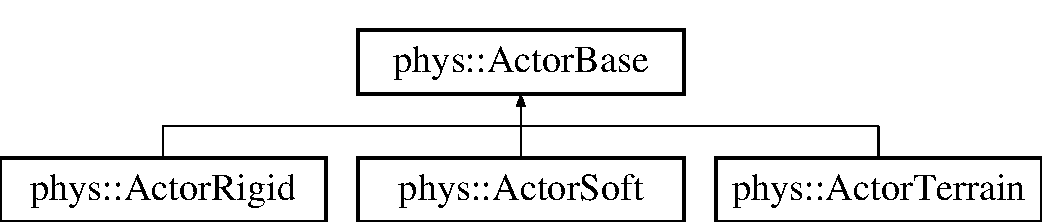
\includegraphics[height=2cm]{d8/d0f/classphys_1_1ActorBase}
\end{center}
\end{figure}
\subsection*{Public Member Functions}
\begin{DoxyCompactItemize}
\item 
virtual \hyperlink{classphys_1_1ActorBase_a5e5d4b50c83c6851e554b5e7ad65403f}{$\sim$ActorBase} ()
\begin{DoxyCompactList}\small\item\em Destructor. \item\end{DoxyCompactList}\item 
\hyperlink{classphys_1_1ActorBase_ad9d90a68921ce81653e9950c1330809d}{ActorBase} (\hyperlink{namespacephys_aa03900411993de7fbfec4789bc1d392e}{String} name, \hyperlink{namespacephys_aa03900411993de7fbfec4789bc1d392e}{String} file, \hyperlink{namespacephys_aa03900411993de7fbfec4789bc1d392e}{String} group, \hyperlink{classphys_1_1World}{World} $\ast$\_\-World)
\begin{DoxyCompactList}\small\item\em Descriptive constructor. \item\end{DoxyCompactList}\item 
void \hyperlink{classphys_1_1ActorBase_a0b0db2ec0f4926326635b86f1ead2276}{SetLocation} (\hyperlink{namespacephys_af7eb897198d265b8e868f45240230d5f}{Real} x, \hyperlink{namespacephys_af7eb897198d265b8e868f45240230d5f}{Real} y, \hyperlink{namespacephys_af7eb897198d265b8e868f45240230d5f}{Real} z)
\begin{DoxyCompactList}\small\item\em Manually sets the location of the actor. \item\end{DoxyCompactList}\item 
void \hyperlink{classphys_1_1ActorBase_a9a182b7262742ab5d499e7a51d407044}{SetLocation} (\hyperlink{classPhysVector3}{PhysVector3} Place)
\begin{DoxyCompactList}\small\item\em Manually sets the location of the actor. \item\end{DoxyCompactList}\item 
\hyperlink{classPhysVector3}{PhysVector3} \hyperlink{classphys_1_1ActorBase_ae402982d8c62acac7a122f24a289731d}{GetLocation} ()
\begin{DoxyCompactList}\small\item\em Retrieves the location of the object. \item\end{DoxyCompactList}\item 
void \hyperlink{classphys_1_1ActorBase_ab7513e8b650b40ea4387c170929457a7}{SetInitLocation} (\hyperlink{classPhysVector3}{PhysVector3} Location)
\begin{DoxyCompactList}\small\item\em Sets the starting location of the actor. \item\end{DoxyCompactList}\item 
void \hyperlink{classphys_1_1ActorBase_a681186465db767954ca3f9530a1d7c36}{SetInitOrientation} (\hyperlink{classphys_1_1Quaternion}{Quaternion} Orientation)
\begin{DoxyCompactList}\small\item\em Sets the starting orientation of the actor. \item\end{DoxyCompactList}\item 
void \hyperlink{classphys_1_1ActorBase_adbf0cc77031f22597a799fd0f7f8216d}{SetOrientation} (\hyperlink{namespacephys_af7eb897198d265b8e868f45240230d5f}{Real} x, \hyperlink{namespacephys_af7eb897198d265b8e868f45240230d5f}{Real} y, \hyperlink{namespacephys_af7eb897198d265b8e868f45240230d5f}{Real} z, \hyperlink{namespacephys_af7eb897198d265b8e868f45240230d5f}{Real} w)
\begin{DoxyCompactList}\small\item\em Sets the orientation of the actor. \item\end{DoxyCompactList}\item 
void \hyperlink{classphys_1_1ActorBase_ac4b0bf1eff730d94f72d04957efea69d}{SetOrientation} (\hyperlink{classphys_1_1Quaternion}{Quaternion} Rotation)
\begin{DoxyCompactList}\small\item\em Sets the orientation of the actor. \item\end{DoxyCompactList}\item 
void \hyperlink{classphys_1_1ActorBase_acd5613286ec14fb2a8e5ed5f5003dc5f}{SetKinematic} ()
\begin{DoxyCompactList}\small\item\em Sets the state of the object to Kinematic. \item\end{DoxyCompactList}\item 
void \hyperlink{classphys_1_1ActorBase_af0219532fe71d1d84042a20a88fe5037}{SetStatic} ()
\begin{DoxyCompactList}\small\item\em Sets the state of the object to Static. \item\end{DoxyCompactList}\end{DoxyCompactItemize}
\subsection*{Protected Member Functions}
\begin{DoxyCompactItemize}
\item 
virtual void \hyperlink{classphys_1_1ActorBase_ac5d4ad5a634b16000742f506ed5957fb}{AddObjectToWorld} (\hyperlink{classphys_1_1World}{World} $\ast$TargetWorld, btSoftRigidDynamicsWorld $\ast$btWorld)=0
\begin{DoxyCompactList}\small\item\em Adds the actor to the physics world. \item\end{DoxyCompactList}\item 
btTriangleMesh $\ast$ \hyperlink{classphys_1_1ActorBase_a4d2137276c50bbe5bc8cf9ecc66581b7}{CreateTrimesh} ()
\begin{DoxyCompactList}\small\item\em Creates a trimesh shape from the mesh file. \item\end{DoxyCompactList}\item 
void \hyperlink{classphys_1_1ActorBase_aff7dbb190fb982a43123bee3066501c4}{CreateEntity} (\hyperlink{namespacephys_aa03900411993de7fbfec4789bc1d392e}{String} name, \hyperlink{namespacephys_aa03900411993de7fbfec4789bc1d392e}{String} file, \hyperlink{namespacephys_aa03900411993de7fbfec4789bc1d392e}{String} group)
\begin{DoxyCompactList}\small\item\em Creates an entity for the mesh file to be placed on a scene node. \item\end{DoxyCompactList}\item 
void \hyperlink{classphys_1_1ActorBase_a125d6f0a0b4072e64490638c074eea2d}{CreateSceneNode} ()
\begin{DoxyCompactList}\small\item\em Creates a node for the entity in the graphical world. \item\end{DoxyCompactList}\item 
void \hyperlink{classphys_1_1ActorBase_af8a6cb524bda889b7a38f0245a7381fb}{SetOgreLocation} (\hyperlink{classPhysVector3}{PhysVector3} Place)
\begin{DoxyCompactList}\small\item\em Sets the location of the graphical body. \item\end{DoxyCompactList}\item 
\hyperlink{classPhysVector3}{PhysVector3} \hyperlink{classphys_1_1ActorBase_a52a65d23c76c805f4851191b62712ed8}{GetOgreLocation} ()
\begin{DoxyCompactList}\small\item\em Retrieves the location of the graphical body. \item\end{DoxyCompactList}\item 
void \hyperlink{classphys_1_1ActorBase_a7b2d13cb1e8bba60eeae782a53fd5e49}{SetOgreOrientation} (\hyperlink{classphys_1_1Quaternion}{Quaternion} Rotation)
\begin{DoxyCompactList}\small\item\em Sets the orientation of the graphical body. \item\end{DoxyCompactList}\item 
void \hyperlink{classphys_1_1ActorBase_a45f190cb9b647bb3385d1298f9dab589}{AttachToGraphics} ()
\begin{DoxyCompactList}\small\item\em Makes the actor visable. \item\end{DoxyCompactList}\item 
virtual void \hyperlink{classphys_1_1ActorBase_ab8d8c68937ea92b245b411c07b8bde7a}{SetBulletLocation} (\hyperlink{classPhysVector3}{PhysVector3} Location)
\begin{DoxyCompactList}\small\item\em Sets the location of the physics body. \item\end{DoxyCompactList}\item 
virtual \hyperlink{classPhysVector3}{PhysVector3} \hyperlink{classphys_1_1ActorBase_ac7c8bbb4859668d71325a791c88584ae}{GetBulletLocation} ()
\begin{DoxyCompactList}\small\item\em Retrieves the location of the physics body. \item\end{DoxyCompactList}\item 
virtual void \hyperlink{classphys_1_1ActorBase_a492244ac46ced53b809f436da992bc84}{SetBulletOrientation} (\hyperlink{classphys_1_1Quaternion}{Quaternion} Rotation)
\begin{DoxyCompactList}\small\item\em Sets the orientation of the physics body. \item\end{DoxyCompactList}\end{DoxyCompactItemize}
\subsection*{Protected Attributes}
\begin{DoxyCompactItemize}
\item 
\hypertarget{classphys_1_1ActorBase_a0ffbb74296ac96db26c890274df794a2}{
\hyperlink{classphys_1_1World}{World} $\ast$ \hyperlink{classphys_1_1ActorBase_a0ffbb74296ac96db26c890274df794a2}{GameWorld}}
\label{d8/d0f/classphys_1_1ActorBase_a0ffbb74296ac96db26c890274df794a2}

\begin{DoxyCompactList}\small\item\em A pointer to the \hyperlink{classphys_1_1World}{World} the actor will reside. \item\end{DoxyCompactList}\item 
\hypertarget{classphys_1_1ActorBase_ae44969ba242ca5c13a608b7467be0674}{
Ogre::Entity $\ast$ \hyperlink{classphys_1_1ActorBase_ae44969ba242ca5c13a608b7467be0674}{entity}}
\label{d8/d0f/classphys_1_1ActorBase_ae44969ba242ca5c13a608b7467be0674}

\begin{DoxyCompactList}\small\item\em This class encapsulates the functionality of the Ogre::Entity using this. \item\end{DoxyCompactList}\item 
\hypertarget{classphys_1_1ActorBase_a687bfa0cc44adf715651c7ac41a46321}{
Ogre::SceneNode $\ast$ \hyperlink{classphys_1_1ActorBase_a687bfa0cc44adf715651c7ac41a46321}{node}}
\label{d8/d0f/classphys_1_1ActorBase_a687bfa0cc44adf715651c7ac41a46321}

\begin{DoxyCompactList}\small\item\em This class encapsulates the functionality of the Ogre::SceneNode using this. \item\end{DoxyCompactList}\item 
\hypertarget{classphys_1_1ActorBase_a643613ce7abb4b6d4352bab036b7cf69}{
btCollisionShape $\ast$ \hyperlink{classphys_1_1ActorBase_a643613ce7abb4b6d4352bab036b7cf69}{Shape}}
\label{d8/d0f/classphys_1_1ActorBase_a643613ce7abb4b6d4352bab036b7cf69}

\begin{DoxyCompactList}\small\item\em This class encapsulates the functionality of the btCollisionShape using this. \item\end{DoxyCompactList}\item 
\hypertarget{classphys_1_1ActorBase_a70676c52ffee64705a7b463d29b60429}{
btCollisionObject $\ast$ \hyperlink{classphys_1_1ActorBase_a70676c52ffee64705a7b463d29b60429}{CollisionObject}}
\label{d8/d0f/classphys_1_1ActorBase_a70676c52ffee64705a7b463d29b60429}

\begin{DoxyCompactList}\small\item\em This class encapsulates the functionality of the btCollisionObject using this. \item\end{DoxyCompactList}\item 
\hypertarget{classphys_1_1ActorBase_a44934cb1db748c3c69e3b88a8dd17dcb}{
\hyperlink{classphys_1_1PhysMotionState}{PhysMotionState} $\ast$ \hyperlink{classphys_1_1ActorBase_a44934cb1db748c3c69e3b88a8dd17dcb}{MotionState}}
\label{d8/d0f/classphys_1_1ActorBase_a44934cb1db748c3c69e3b88a8dd17dcb}

\begin{DoxyCompactList}\small\item\em This class encapsulates the functionality of the \hyperlink{classphys_1_1PhysMotionState}{PhysMotionState} using this. \item\end{DoxyCompactList}\end{DoxyCompactItemize}
\subsection*{Friends}
\begin{DoxyCompactItemize}
\item 
\hypertarget{classphys_1_1ActorBase_ae18d4e9935739ce8709d2974a7e91b16}{
class \hyperlink{classphys_1_1ActorBase_ae18d4e9935739ce8709d2974a7e91b16}{phys::World}}
\label{d8/d0f/classphys_1_1ActorBase_ae18d4e9935739ce8709d2974a7e91b16}

\end{DoxyCompactItemize}


\subsection{Detailed Description}
This is the base class from which all the actors inherit. The actor classes store and manage all the relevant data regarding objects inside the \hyperlink{classphys_1_1World}{World}. They serve as a binder between the physics and graphics for objects and have functions that allow the manipulation of objects loaded into the \hyperlink{classphys_1_1World}{World}. Currently there are 4 actor classes: \hyperlink{classphys_1_1ActorBase}{ActorBase}, ActorDynRigid, ActorDynSoft, and ActorSta. \par
 \hyperlink{classphys_1_1ActorBase}{ActorBase} is a base class that serves as a template for the other three actor classes. \par
 \hyperlink{classphys_1_1ActorBase}{ActorBase} should never be created, as it lacks the functionality needed for most objects. 

Definition at line 92 of file physactor.h.



\subsection{Constructor \& Destructor Documentation}
\hypertarget{classphys_1_1ActorBase_a5e5d4b50c83c6851e554b5e7ad65403f}{
\index{phys::ActorBase@{phys::ActorBase}!$\sim$ActorBase@{$\sim$ActorBase}}
\index{$\sim$ActorBase@{$\sim$ActorBase}!phys::ActorBase@{phys::ActorBase}}
\subsubsection[{$\sim$ActorBase}]{\setlength{\rightskip}{0pt plus 5cm}phys::ActorBase::$\sim$ActorBase ()\hspace{0.3cm}{\ttfamily  \mbox{[}virtual\mbox{]}}}}
\label{d8/d0f/classphys_1_1ActorBase_a5e5d4b50c83c6851e554b5e7ad65403f}


Destructor. 

The class destructor. 

Definition at line 120 of file physactor.cpp.

\hypertarget{classphys_1_1ActorBase_ad9d90a68921ce81653e9950c1330809d}{
\index{phys::ActorBase@{phys::ActorBase}!ActorBase@{ActorBase}}
\index{ActorBase@{ActorBase}!phys::ActorBase@{phys::ActorBase}}
\subsubsection[{ActorBase}]{\setlength{\rightskip}{0pt plus 5cm}phys::ActorBase::ActorBase ({\bf String} {\em name}, \/  {\bf String} {\em file}, \/  {\bf String} {\em group}, \/  {\bf World} $\ast$ {\em \_\-World})}}
\label{d8/d0f/classphys_1_1ActorBase_ad9d90a68921ce81653e9950c1330809d}


Descriptive constructor. 

This constructor contains the basic information needed to make an actor. 
\begin{DoxyParams}{Parameters}
\item[{\em name}]The name of the actor. \item[{\em file}]The 3d mesh file that contains the 3d model the actor will use. \item[{\em group}]The resource group where the 3d mesh and other related files can be found. \item[{\em \_\-World}]Pointer to the \hyperlink{classphys_1_1World}{World} this object will be added to. \end{DoxyParams}


Definition at line 110 of file physactor.cpp.



\subsection{Member Function Documentation}
\hypertarget{classphys_1_1ActorBase_ac5d4ad5a634b16000742f506ed5957fb}{
\index{phys::ActorBase@{phys::ActorBase}!AddObjectToWorld@{AddObjectToWorld}}
\index{AddObjectToWorld@{AddObjectToWorld}!phys::ActorBase@{phys::ActorBase}}
\subsubsection[{AddObjectToWorld}]{\setlength{\rightskip}{0pt plus 5cm}virtual void phys::ActorBase::AddObjectToWorld ({\bf World} $\ast$ {\em TargetWorld}, \/  btSoftRigidDynamicsWorld $\ast$ {\em btWorld})\hspace{0.3cm}{\ttfamily  \mbox{[}protected, pure virtual\mbox{]}}}}
\label{d8/d0f/classphys_1_1ActorBase_ac5d4ad5a634b16000742f506ed5957fb}


Adds the actor to the physics world. 

Adds the actor to the physics world. \par
 This is automaticly called by the PhysWorlds AddActor function and shouldn't be called manually. 
\begin{DoxyParams}{Parameters}
\item[{\em TargetWorld}]Pointer to the \hyperlink{classphys_1_1World}{World} class. \item[{\em btWorld}]Pointer to the physics world. \end{DoxyParams}


Implemented in \hyperlink{classphys_1_1ActorRigid_a3c56eb06fe6a7d468b7a67c45ade7be4}{phys::ActorRigid}, and \hyperlink{classphys_1_1ActorSoft_a3a704ab32f847a5d0e060f8a592efefd}{phys::ActorSoft}.

\hypertarget{classphys_1_1ActorBase_a45f190cb9b647bb3385d1298f9dab589}{
\index{phys::ActorBase@{phys::ActorBase}!AttachToGraphics@{AttachToGraphics}}
\index{AttachToGraphics@{AttachToGraphics}!phys::ActorBase@{phys::ActorBase}}
\subsubsection[{AttachToGraphics}]{\setlength{\rightskip}{0pt plus 5cm}void phys::ActorBase::AttachToGraphics ()\hspace{0.3cm}{\ttfamily  \mbox{[}protected\mbox{]}}}}
\label{d8/d0f/classphys_1_1ActorBase_a45f190cb9b647bb3385d1298f9dab589}


Makes the actor visable. 

Adds the actor to all the nessessary graphics elements to make it visable on screen. \par
 This is automaticly called by the PhysWorlds AddActor function and shouldn't ever need to be called manually. 

Definition at line 321 of file physactor.cpp.

\hypertarget{classphys_1_1ActorBase_aff7dbb190fb982a43123bee3066501c4}{
\index{phys::ActorBase@{phys::ActorBase}!CreateEntity@{CreateEntity}}
\index{CreateEntity@{CreateEntity}!phys::ActorBase@{phys::ActorBase}}
\subsubsection[{CreateEntity}]{\setlength{\rightskip}{0pt plus 5cm}void phys::ActorBase::CreateEntity ({\bf String} {\em name}, \/  {\bf String} {\em file}, \/  {\bf String} {\em group})\hspace{0.3cm}{\ttfamily  \mbox{[}protected\mbox{]}}}}
\label{d8/d0f/classphys_1_1ActorBase_aff7dbb190fb982a43123bee3066501c4}


Creates an entity for the mesh file to be placed on a scene node. 

Creates an entity in the scene manager from the mesh file provided to be attached to a node in the graphical world. \par
 This function is called on by the Constructor, and shouldn't be called manually. 
\begin{DoxyParams}{Parameters}
\item[{\em name}]Name of the actor. \item[{\em file}]File name of the graphical mesh to be used. \item[{\em group}]Resource group where the graphical mesh can be found. \end{DoxyParams}


Definition at line 220 of file physactor.cpp.

\hypertarget{classphys_1_1ActorBase_a125d6f0a0b4072e64490638c074eea2d}{
\index{phys::ActorBase@{phys::ActorBase}!CreateSceneNode@{CreateSceneNode}}
\index{CreateSceneNode@{CreateSceneNode}!phys::ActorBase@{phys::ActorBase}}
\subsubsection[{CreateSceneNode}]{\setlength{\rightskip}{0pt plus 5cm}void phys::ActorBase::CreateSceneNode ()\hspace{0.3cm}{\ttfamily  \mbox{[}protected\mbox{]}}}}
\label{d8/d0f/classphys_1_1ActorBase_a125d6f0a0b4072e64490638c074eea2d}


Creates a node for the entity in the graphical world. 

Creates a node in the scene manager to attach the actor's entity to within the graphical world. \par
 This function is called on by the Constructor, and shouldn't be called manually. 

Definition at line 225 of file physactor.cpp.

\hypertarget{classphys_1_1ActorBase_a4d2137276c50bbe5bc8cf9ecc66581b7}{
\index{phys::ActorBase@{phys::ActorBase}!CreateTrimesh@{CreateTrimesh}}
\index{CreateTrimesh@{CreateTrimesh}!phys::ActorBase@{phys::ActorBase}}
\subsubsection[{CreateTrimesh}]{\setlength{\rightskip}{0pt plus 5cm}btTriangleMesh $\ast$ phys::ActorBase::CreateTrimesh ()\hspace{0.3cm}{\ttfamily  \mbox{[}protected\mbox{]}}}}
\label{d8/d0f/classphys_1_1ActorBase_a4d2137276c50bbe5bc8cf9ecc66581b7}


Creates a trimesh shape from the mesh file. 

Makes a trimesh to be used as a collision shape in the physics world from a mesh file. \par
 This is automaticly called by the CreateShapeFromMesh function in child classes and shouldn't be called manually. 

Definition at line 129 of file physactor.cpp.

\hypertarget{classphys_1_1ActorBase_ac7c8bbb4859668d71325a791c88584ae}{
\index{phys::ActorBase@{phys::ActorBase}!GetBulletLocation@{GetBulletLocation}}
\index{GetBulletLocation@{GetBulletLocation}!phys::ActorBase@{phys::ActorBase}}
\subsubsection[{GetBulletLocation}]{\setlength{\rightskip}{0pt plus 5cm}{\bf PhysVector3} phys::ActorBase::GetBulletLocation ()\hspace{0.3cm}{\ttfamily  \mbox{[}protected, virtual\mbox{]}}}}
\label{d8/d0f/classphys_1_1ActorBase_ac7c8bbb4859668d71325a791c88584ae}


Retrieves the location of the physics body. 

This function will retrieve the location of the object within the physics world. 

Definition at line 251 of file physactor.cpp.

\hypertarget{classphys_1_1ActorBase_ae402982d8c62acac7a122f24a289731d}{
\index{phys::ActorBase@{phys::ActorBase}!GetLocation@{GetLocation}}
\index{GetLocation@{GetLocation}!phys::ActorBase@{phys::ActorBase}}
\subsubsection[{GetLocation}]{\setlength{\rightskip}{0pt plus 5cm}{\bf PhysVector3} phys::ActorBase::GetLocation ()}}
\label{d8/d0f/classphys_1_1ActorBase_ae402982d8c62acac7a122f24a289731d}


Retrieves the location of the object. 

This function will retrieve the location of the object within the world. 

Definition at line 288 of file physactor.cpp.

\hypertarget{classphys_1_1ActorBase_a52a65d23c76c805f4851191b62712ed8}{
\index{phys::ActorBase@{phys::ActorBase}!GetOgreLocation@{GetOgreLocation}}
\index{GetOgreLocation@{GetOgreLocation}!phys::ActorBase@{phys::ActorBase}}
\subsubsection[{GetOgreLocation}]{\setlength{\rightskip}{0pt plus 5cm}{\bf PhysVector3} phys::ActorBase::GetOgreLocation ()\hspace{0.3cm}{\ttfamily  \mbox{[}protected\mbox{]}}}}
\label{d8/d0f/classphys_1_1ActorBase_a52a65d23c76c805f4851191b62712ed8}


Retrieves the location of the graphical body. 

This function will retrieve the location of the object within the graphical world. 

Definition at line 238 of file physactor.cpp.

\hypertarget{classphys_1_1ActorBase_ab8d8c68937ea92b245b411c07b8bde7a}{
\index{phys::ActorBase@{phys::ActorBase}!SetBulletLocation@{SetBulletLocation}}
\index{SetBulletLocation@{SetBulletLocation}!phys::ActorBase@{phys::ActorBase}}
\subsubsection[{SetBulletLocation}]{\setlength{\rightskip}{0pt plus 5cm}void phys::ActorBase::SetBulletLocation ({\bf PhysVector3} {\em Location})\hspace{0.3cm}{\ttfamily  \mbox{[}protected, virtual\mbox{]}}}}
\label{d8/d0f/classphys_1_1ActorBase_ab8d8c68937ea92b245b411c07b8bde7a}


Sets the location of the physics body. 

This will take a \hyperlink{classPhysVector3}{PhysVector3} and set the location of the actor within the physics world. \par
 This function is called on by the SetLocation function, and shouldn't be called manually. 
\begin{DoxyParams}{Parameters}
\item[{\em Location}]The \hyperlink{classPhysVector3}{PhysVector3} representing the location. \end{DoxyParams}


Definition at line 245 of file physactor.cpp.

\hypertarget{classphys_1_1ActorBase_a492244ac46ced53b809f436da992bc84}{
\index{phys::ActorBase@{phys::ActorBase}!SetBulletOrientation@{SetBulletOrientation}}
\index{SetBulletOrientation@{SetBulletOrientation}!phys::ActorBase@{phys::ActorBase}}
\subsubsection[{SetBulletOrientation}]{\setlength{\rightskip}{0pt plus 5cm}void phys::ActorBase::SetBulletOrientation ({\bf Quaternion} {\em Rotation})\hspace{0.3cm}{\ttfamily  \mbox{[}protected, virtual\mbox{]}}}}
\label{d8/d0f/classphys_1_1ActorBase_a492244ac46ced53b809f436da992bc84}


Sets the orientation of the physics body. 

This will take a PhysQuaternion and set the orientation of the actor within the physics world. \par
 This function is called on by the SetOrientation function, and shouldn't be called manually. 
\begin{DoxyParams}{Parameters}
\item[{\em Rotation}]The quaternion representing the rotation of the actor. \end{DoxyParams}


Definition at line 267 of file physactor.cpp.

\hypertarget{classphys_1_1ActorBase_ab7513e8b650b40ea4387c170929457a7}{
\index{phys::ActorBase@{phys::ActorBase}!SetInitLocation@{SetInitLocation}}
\index{SetInitLocation@{SetInitLocation}!phys::ActorBase@{phys::ActorBase}}
\subsubsection[{SetInitLocation}]{\setlength{\rightskip}{0pt plus 5cm}void phys::ActorBase::SetInitLocation ({\bf PhysVector3} {\em Location})}}
\label{d8/d0f/classphys_1_1ActorBase_ab7513e8b650b40ea4387c170929457a7}


Sets the starting location of the actor. 

Calling this function after adding it to the \hyperlink{classphys_1_1World}{World} will have no effect. \par
 This function will set where the actor will be located in the \hyperlink{classphys_1_1World}{World} when it is first placed inside the world. 
\begin{DoxyParams}{Parameters}
\item[{\em Location}]The \hyperlink{classPhysVector3}{PhysVector3} representing the location. \end{DoxyParams}


Definition at line 293 of file physactor.cpp.

\hypertarget{classphys_1_1ActorBase_a681186465db767954ca3f9530a1d7c36}{
\index{phys::ActorBase@{phys::ActorBase}!SetInitOrientation@{SetInitOrientation}}
\index{SetInitOrientation@{SetInitOrientation}!phys::ActorBase@{phys::ActorBase}}
\subsubsection[{SetInitOrientation}]{\setlength{\rightskip}{0pt plus 5cm}void phys::ActorBase::SetInitOrientation ({\bf Quaternion} {\em Orientation})}}
\label{d8/d0f/classphys_1_1ActorBase_a681186465db767954ca3f9530a1d7c36}


Sets the starting orientation of the actor. 

Calling this function after adding it to the \hyperlink{classphys_1_1World}{World} will have no effect. \par
 This function will set where the actor is facing in the \hyperlink{classphys_1_1World}{World} when it is first placed inside the world. 
\begin{DoxyParams}{Parameters}
\item[{\em Orientation}]The PhysQuaternion representing the Orientation. \end{DoxyParams}


Definition at line 301 of file physactor.cpp.

\hypertarget{classphys_1_1ActorBase_acd5613286ec14fb2a8e5ed5f5003dc5f}{
\index{phys::ActorBase@{phys::ActorBase}!SetKinematic@{SetKinematic}}
\index{SetKinematic@{SetKinematic}!phys::ActorBase@{phys::ActorBase}}
\subsubsection[{SetKinematic}]{\setlength{\rightskip}{0pt plus 5cm}void phys::ActorBase::SetKinematic ()}}
\label{d8/d0f/classphys_1_1ActorBase_acd5613286ec14fb2a8e5ed5f5003dc5f}


Sets the state of the object to Kinematic. 

This function will set the object to a Kinematic Object. \par
 Kinematic Objects are like Static Objects but are also able to be moved directly by character controllers. 

Definition at line 333 of file physactor.cpp.

\hypertarget{classphys_1_1ActorBase_a9a182b7262742ab5d499e7a51d407044}{
\index{phys::ActorBase@{phys::ActorBase}!SetLocation@{SetLocation}}
\index{SetLocation@{SetLocation}!phys::ActorBase@{phys::ActorBase}}
\subsubsection[{SetLocation}]{\setlength{\rightskip}{0pt plus 5cm}void phys::ActorBase::SetLocation ({\bf PhysVector3} {\em Place})}}
\label{d8/d0f/classphys_1_1ActorBase_a9a182b7262742ab5d499e7a51d407044}


Manually sets the location of the actor. 

Calling this function prior to adding it to the \hyperlink{classphys_1_1World}{World} will have no effect. \par
 In most situations you won't want to use this function, and instead produce movement through physics functions. 
\begin{DoxyParams}{Parameters}
\item[{\em Place}]The \hyperlink{classPhysVector3}{PhysVector3} representing the location. \end{DoxyParams}


Definition at line 282 of file physactor.cpp.

\hypertarget{classphys_1_1ActorBase_a0b0db2ec0f4926326635b86f1ead2276}{
\index{phys::ActorBase@{phys::ActorBase}!SetLocation@{SetLocation}}
\index{SetLocation@{SetLocation}!phys::ActorBase@{phys::ActorBase}}
\subsubsection[{SetLocation}]{\setlength{\rightskip}{0pt plus 5cm}void phys::ActorBase::SetLocation ({\bf Real} {\em x}, \/  {\bf Real} {\em y}, \/  {\bf Real} {\em z})}}
\label{d8/d0f/classphys_1_1ActorBase_a0b0db2ec0f4926326635b86f1ead2276}


Manually sets the location of the actor. 

Calling this function prior to adding it to the \hyperlink{classphys_1_1World}{World} will have no effect. \par
 In most situations you won't want to use this function, and instead produce movement through physics functions. 
\begin{DoxyParams}{Parameters}
\item[{\em x}]Location on the X vector. \item[{\em y}]Location on the Y vector. \item[{\em z}]Location on the Z vector. \end{DoxyParams}


Definition at line 276 of file physactor.cpp.

\hypertarget{classphys_1_1ActorBase_af8a6cb524bda889b7a38f0245a7381fb}{
\index{phys::ActorBase@{phys::ActorBase}!SetOgreLocation@{SetOgreLocation}}
\index{SetOgreLocation@{SetOgreLocation}!phys::ActorBase@{phys::ActorBase}}
\subsubsection[{SetOgreLocation}]{\setlength{\rightskip}{0pt plus 5cm}void phys::ActorBase::SetOgreLocation ({\bf PhysVector3} {\em Place})\hspace{0.3cm}{\ttfamily  \mbox{[}protected\mbox{]}}}}
\label{d8/d0f/classphys_1_1ActorBase_af8a6cb524bda889b7a38f0245a7381fb}


Sets the location of the graphical body. 

This will take a \hyperlink{classPhysVector3}{PhysVector3} and set the location of the actor within the graphical world. \par
 This function is called on by the SetLocation function, and shouldn't be called manually. 
\begin{DoxyParams}{Parameters}
\item[{\em Place}]The \hyperlink{classPhysVector3}{PhysVector3} representing the location. \end{DoxyParams}


Definition at line 233 of file physactor.cpp.

\hypertarget{classphys_1_1ActorBase_a7b2d13cb1e8bba60eeae782a53fd5e49}{
\index{phys::ActorBase@{phys::ActorBase}!SetOgreOrientation@{SetOgreOrientation}}
\index{SetOgreOrientation@{SetOgreOrientation}!phys::ActorBase@{phys::ActorBase}}
\subsubsection[{SetOgreOrientation}]{\setlength{\rightskip}{0pt plus 5cm}void phys::ActorBase::SetOgreOrientation ({\bf Quaternion} {\em Rotation})\hspace{0.3cm}{\ttfamily  \mbox{[}protected\mbox{]}}}}
\label{d8/d0f/classphys_1_1ActorBase_a7b2d13cb1e8bba60eeae782a53fd5e49}


Sets the orientation of the graphical body. 

This will take a PhysQuaternion and set the orientation of the actor within the graphical world. \par
 This function is called on by the SetOrientation function, and shouldn't be called manually. 
\begin{DoxyParams}{Parameters}
\item[{\em Rotation}]The quaternion representing the rotation of the actor. \end{DoxyParams}


Definition at line 262 of file physactor.cpp.

\hypertarget{classphys_1_1ActorBase_ac4b0bf1eff730d94f72d04957efea69d}{
\index{phys::ActorBase@{phys::ActorBase}!SetOrientation@{SetOrientation}}
\index{SetOrientation@{SetOrientation}!phys::ActorBase@{phys::ActorBase}}
\subsubsection[{SetOrientation}]{\setlength{\rightskip}{0pt plus 5cm}void phys::ActorBase::SetOrientation ({\bf Quaternion} {\em Rotation})}}
\label{d8/d0f/classphys_1_1ActorBase_ac4b0bf1eff730d94f72d04957efea69d}


Sets the orientation of the actor. 

Sets the orientation of the actor via a \hyperlink{classphys_1_1Quaternion}{Quaternion}. 
\begin{DoxyParams}{Parameters}
\item[{\em Rotation}]The \hyperlink{classphys_1_1Quaternion}{Quaternion} representing the Rotation. \end{DoxyParams}


Definition at line 312 of file physactor.cpp.

\hypertarget{classphys_1_1ActorBase_adbf0cc77031f22597a799fd0f7f8216d}{
\index{phys::ActorBase@{phys::ActorBase}!SetOrientation@{SetOrientation}}
\index{SetOrientation@{SetOrientation}!phys::ActorBase@{phys::ActorBase}}
\subsubsection[{SetOrientation}]{\setlength{\rightskip}{0pt plus 5cm}void phys::ActorBase::SetOrientation ({\bf Real} {\em x}, \/  {\bf Real} {\em y}, \/  {\bf Real} {\em z}, \/  {\bf Real} {\em w})}}
\label{d8/d0f/classphys_1_1ActorBase_adbf0cc77031f22597a799fd0f7f8216d}


Sets the orientation of the actor. 

Sets the orientation of the actor via \hyperlink{classphys_1_1Quaternion}{Quaternion} parameters. 
\begin{DoxyParams}{Parameters}
\item[{\em x}]Where the X vector is rotated about. \item[{\em y}]Where the Y vector is rotated about. \item[{\em z}]Where the Z vector is rotated about. \item[{\em w}]How much to about the x, y, z. \end{DoxyParams}


Definition at line 306 of file physactor.cpp.

\hypertarget{classphys_1_1ActorBase_af0219532fe71d1d84042a20a88fe5037}{
\index{phys::ActorBase@{phys::ActorBase}!SetStatic@{SetStatic}}
\index{SetStatic@{SetStatic}!phys::ActorBase@{phys::ActorBase}}
\subsubsection[{SetStatic}]{\setlength{\rightskip}{0pt plus 5cm}void phys::ActorBase::SetStatic ()}}
\label{d8/d0f/classphys_1_1ActorBase_af0219532fe71d1d84042a20a88fe5037}


Sets the state of the object to Static. 

This function will set the object to a Static Object. \par
 Static Objects don't move or have any force applied to them, but are cabable of exerting force on other objects. 

Definition at line 339 of file physactor.cpp.



The documentation for this class was generated from the following files:\begin{DoxyCompactItemize}
\item 
physactor.h\item 
physactor.cpp\end{DoxyCompactItemize}

\hypertarget{classphys_1_1ActorContainerBase}{
\subsection{phys::ActorContainerBase Class Reference}
\label{classphys_1_1ActorContainerBase}\index{phys::ActorContainerBase@{phys::ActorContainerBase}}
}


A base class to unify the interface for different kinds of containers for holding actors.  




{\ttfamily \#include $<$actorcontainerbase.h$>$}

Inheritance diagram for phys::ActorContainerBase:\begin{figure}[H]
\begin{center}
\leavevmode
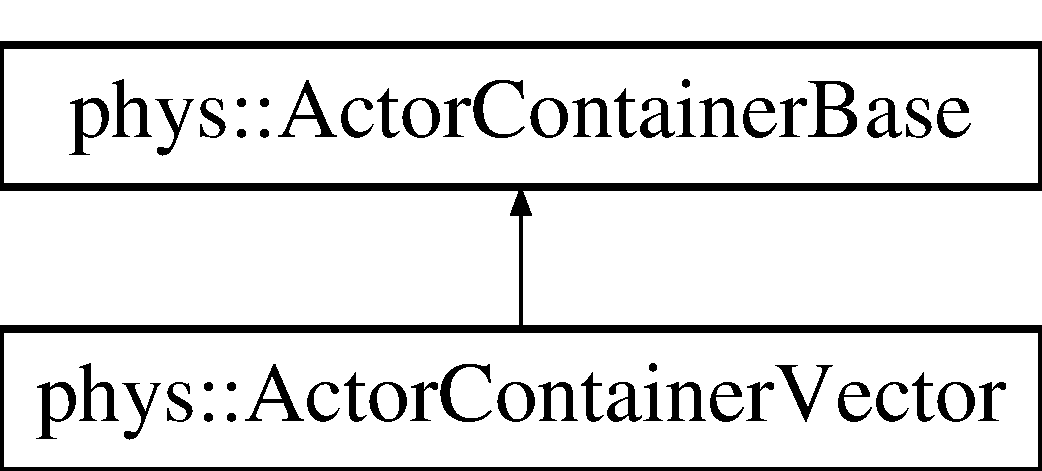
\includegraphics[height=2.000000cm]{classphys_1_1ActorContainerBase}
\end{center}
\end{figure}
\subsubsection*{Public Member Functions}
\begin{DoxyCompactItemize}
\item 
\hyperlink{classphys_1_1ActorContainerBase_ac17a442ad8aacba14d1cef956c0ddbb8}{ActorContainerBase} ()
\begin{DoxyCompactList}\small\item\em Basic Constructor. \item\end{DoxyCompactList}\item 
virtual \hyperlink{classphys_1_1ActorContainerBase_aa5eac062dd70a220a4ec6df973c6f258}{$\sim$ActorContainerBase} ()
\begin{DoxyCompactList}\small\item\em Destructor. \item\end{DoxyCompactList}\item 
virtual void \hyperlink{classphys_1_1ActorContainerBase_a8dd213cba4915f68ac421fc9f341cbbe}{AddActor} (\hyperlink{classphys_1_1ActorBase}{ActorBase} $\ast$ActorToAdd)=0
\begin{DoxyCompactList}\small\item\em This will add an Actor to this container and the world. \item\end{DoxyCompactList}\item 
virtual \hyperlink{classphys_1_1ActorBase}{ActorBase} $\ast$ \hyperlink{classphys_1_1ActorContainerBase_a6ccc6d058bcbbe0b9a638e28fb136477}{LastActorAdded} ()=0
\begin{DoxyCompactList}\small\item\em This provides an easy way to access the last Actor added to this container. \item\end{DoxyCompactList}\item 
virtual void \hyperlink{classphys_1_1ActorContainerBase_a523072e42f6b581d044432f84a84ede4}{RemoveActor} (\hyperlink{classphys_1_1ActorBase}{ActorBase} $\ast$ActorToRemove)=0
\begin{DoxyCompactList}\small\item\em Remove an Actor. \item\end{DoxyCompactList}\item 
virtual void \hyperlink{classphys_1_1ActorContainerBase_a60f37a056e8750f3b389c5ceed14520c}{RemoveActorAtCursor} ()=0
\begin{DoxyCompactList}\small\item\em Removes the current actor. \item\end{DoxyCompactList}\item 
\hypertarget{classphys_1_1ActorContainerBase_abc75d53e24ca0d9c2d9dcd14f6107149}{
virtual void \hyperlink{classphys_1_1ActorContainerBase_abc75d53e24ca0d9c2d9dcd14f6107149}{RemoveAllActors} ()=0}
\label{classphys_1_1ActorContainerBase_abc75d53e24ca0d9c2d9dcd14f6107149}

\begin{DoxyCompactList}\small\item\em Clears this container of all actors it is storing. \item\end{DoxyCompactList}\item 
virtual \hyperlink{namespacephys_a460f6bc24c8dd347b05e0366ae34f34a}{Whole} \hyperlink{classphys_1_1ActorContainerBase_aa5ec651d4634b2d90efe2a76f9d2fbdd}{GetActorCount} () const =0
\begin{DoxyCompactList}\small\item\em Returns how many actors this stores. \item\end{DoxyCompactList}\item 
virtual void \hyperlink{classphys_1_1ActorContainerBase_ab1a44758d7c17e70ff2e0f8de47424c3}{CursorToFirst} ()=0
\begin{DoxyCompactList}\small\item\em This moves the cursor to the first item in the container. \item\end{DoxyCompactList}\item 
virtual void \hyperlink{classphys_1_1ActorContainerBase_a7c424168c0bbd973b283a083714123b3}{CursorToPrevious} ()=0
\begin{DoxyCompactList}\small\item\em This moves the cursor to the previous item in the container. \item\end{DoxyCompactList}\item 
virtual void \hyperlink{classphys_1_1ActorContainerBase_a1aa337456a4e74cb5740dbae08778072}{CursorToNext} ()=0
\begin{DoxyCompactList}\small\item\em This moves the cursor to the next item in the container. \item\end{DoxyCompactList}\item 
virtual void \hyperlink{classphys_1_1ActorContainerBase_afad072e018a04c190e5e5fb93b82b354}{CursorToLast} ()=0
\begin{DoxyCompactList}\small\item\em This moves the cursor to the last item in the container. \item\end{DoxyCompactList}\item 
virtual \hyperlink{classphys_1_1ActorBase}{ActorBase} $\ast$ \hyperlink{classphys_1_1ActorContainerBase_a2c8fb86a9e188aece105b2a753ccc19a}{GetAtCursor} () const =0
\begin{DoxyCompactList}\small\item\em This gets the actor at the cursor. \item\end{DoxyCompactList}\item 
virtual \hyperlink{classphys_1_1ActorBase}{ActorBase} $\ast$ \hyperlink{classphys_1_1ActorContainerBase_ae703482d84a9c6726e28a8f26418b161}{GetFirst} () const =0
\begin{DoxyCompactList}\small\item\em This gets the first actor in the container. \item\end{DoxyCompactList}\item 
virtual \hyperlink{classphys_1_1ActorBase}{ActorBase} $\ast$ \hyperlink{classphys_1_1ActorContainerBase_a8efeffd5ae22085fe01af791b3ea559e}{GetLast} () const =0
\begin{DoxyCompactList}\small\item\em This gets the last actor in the container. \item\end{DoxyCompactList}\item 
virtual \hyperlink{classphys_1_1ActorBase}{ActorBase} $\ast$ \hyperlink{classphys_1_1ActorContainerBase_a1ade0001858f87ce1843cc6f6ec4e1c0}{FindActor} (Ogre::SceneNode $\ast$GraphicsNode)=0
\begin{DoxyCompactList}\small\item\em This finds an actor by searching for a graphics subsystem nodes. \item\end{DoxyCompactList}\item 
virtual \hyperlink{classphys_1_1ActorBase}{ActorBase} $\ast$ \hyperlink{classphys_1_1ActorContainerBase_a9ba6e38e0f12ada968cfee72fe5144d4}{FindActor} (btCollisionObject $\ast$PhysicsObject)=0
\begin{DoxyCompactList}\small\item\em This finds an actor by searching for a physics subsystem object. \item\end{DoxyCompactList}\item 
virtual \hyperlink{classphys_1_1ActorBase}{ActorBase} $\ast$ \hyperlink{classphys_1_1ActorContainerBase_a91223cbaebb8e5f11a4f971d7e5b64b6}{FindActor} (\hyperlink{namespacephys_aa03900411993de7fbfec4789bc1d392e}{String} Name)=0
\begin{DoxyCompactList}\small\item\em This finds an actor based on its name. \item\end{DoxyCompactList}\item 
virtual \hyperlink{namespacephys_aa03900411993de7fbfec4789bc1d392e}{String} \hyperlink{classphys_1_1ActorContainerBase_a0ed43bc828aaee8ee33152970c3cc16d}{GetContainerType} () const =0
\begin{DoxyCompactList}\small\item\em Which kind of container it this anyway. \item\end{DoxyCompactList}\item 
virtual \hyperlink{classphys_1_1World}{World} $\ast$ \hyperlink{classphys_1_1ActorContainerBase_a479e6c7434f2611b0cfe6ca1fd4ebdd1}{GetGameWorld} () const =0
\begin{DoxyCompactList}\small\item\em This gets the \hyperlink{classphys_1_1World}{World} that this class is working with. \item\end{DoxyCompactList}\item 
virtual void \hyperlink{classphys_1_1ActorContainerBase_ae0cb5c288f17507247dd98d3a2466876}{SetGameWorld} (\hyperlink{classphys_1_1World}{World} $\ast$GameWorld\_\-)=0
\begin{DoxyCompactList}\small\item\em This sets the \hyperlink{classphys_1_1World}{phys::World} that this Manager works with. \item\end{DoxyCompactList}\item 
virtual void \hyperlink{classphys_1_1ActorContainerBase_a366c1797bef08f3a1846bf010e2e2b04}{SetGameWorld} (\hyperlink{classphys_1_1World}{World} $\ast$GameWorld\_\-, bool AddToWorld, bool RemoveFromWorld)=0
\begin{DoxyCompactList}\small\item\em Optionally move actors into or out of a physworld. \item\end{DoxyCompactList}\end{DoxyCompactItemize}
\subsubsection*{Protected Member Functions}
\begin{DoxyCompactItemize}
\item 
\hypertarget{classphys_1_1ActorContainerBase_a44adf1174e624d9fa1408c9885f9ea12}{
Ogre::SceneNode $\ast$ \hyperlink{classphys_1_1ActorContainerBase_a44adf1174e624d9fa1408c9885f9ea12}{GetNode} (\hyperlink{classphys_1_1ActorBase}{ActorBase} $\ast$actor) const }
\label{classphys_1_1ActorContainerBase_a44adf1174e624d9fa1408c9885f9ea12}

\begin{DoxyCompactList}\small\item\em Used to work around the scenenode of an Actor being private, so all derived Containers can access it. \item\end{DoxyCompactList}\item 
\hypertarget{classphys_1_1ActorContainerBase_a3f3d84f7775d2e8597290e214fedd5f9}{
btCollisionObject $\ast$ \hyperlink{classphys_1_1ActorContainerBase_a3f3d84f7775d2e8597290e214fedd5f9}{GetCollisionObject} (\hyperlink{classphys_1_1ActorBase}{ActorBase} $\ast$actor) const }
\label{classphys_1_1ActorContainerBase_a3f3d84f7775d2e8597290e214fedd5f9}

\begin{DoxyCompactList}\small\item\em Used to work around the collision object of an Actor being private, so all derived Containers can access it. \item\end{DoxyCompactList}\end{DoxyCompactItemize}


\subsubsection{Detailed Description}
A base class to unify the interface for different kinds of containers for holding actors. Containers for actors must implement atleast this interface(abstract base class) to be usable with the \hyperlink{classphys_1_1World}{phys::World} for tracking in game objects. There are several reasons why this will be useful. Our first thought was deriving from this and an STL container like vector or list. Members of this class should be implementing or inheriting a proper container\par
\par
 The phys world will use one of these containers to store all of the actors for tracking purposes Since \par
\par
 In theory you should be be able to work with multiple actor containers and swiftly add or remove them to ad from a world to quickly control what actors are being worked with. It should even be possible to remove all actors, or have multiple set of actor in the world if you use the GameWorldSet methods carefully. \par
\par
 Additionally the is no reason an actor could be in multiple containers so this can provide even more options for actor sorting and categorization at runtime. \par
\par
 Because of this classes representation of a cursor only 1 thread at a time should use the cursor movement functions. For the container that the \hyperlink{classphys_1_1World}{phys::World} keeps it should be assume that the cursor is used. For other containers you should manage you container carefully and/or use another iteration method, such as STL iterators. 

Definition at line 76 of file actorcontainerbase.h.



\subsubsection{Constructor \& Destructor Documentation}
\hypertarget{classphys_1_1ActorContainerBase_ac17a442ad8aacba14d1cef956c0ddbb8}{
\index{phys::ActorContainerBase@{phys::ActorContainerBase}!ActorContainerBase@{ActorContainerBase}}
\index{ActorContainerBase@{ActorContainerBase}!phys::ActorContainerBase@{phys::ActorContainerBase}}
\paragraph[{ActorContainerBase}]{\setlength{\rightskip}{0pt plus 5cm}phys::ActorContainerBase::ActorContainerBase (
\begin{DoxyParamCaption}
{}
\end{DoxyParamCaption}
)}\hfill}
\label{classphys_1_1ActorContainerBase_ac17a442ad8aacba14d1cef956c0ddbb8}


Basic Constructor. 

This just assigned the passed pointer to ParentWorld 

Definition at line 54 of file actorcontainerbase.cpp.

\hypertarget{classphys_1_1ActorContainerBase_aa5eac062dd70a220a4ec6df973c6f258}{
\index{phys::ActorContainerBase@{phys::ActorContainerBase}!$\sim$ActorContainerBase@{$\sim$ActorContainerBase}}
\index{$\sim$ActorContainerBase@{$\sim$ActorContainerBase}!phys::ActorContainerBase@{phys::ActorContainerBase}}
\paragraph[{$\sim$ActorContainerBase}]{\setlength{\rightskip}{0pt plus 5cm}phys::ActorContainerBase::$\sim$ActorContainerBase (
\begin{DoxyParamCaption}
{}
\end{DoxyParamCaption}
)\hspace{0.3cm}{\ttfamily  \mbox{[}virtual\mbox{]}}}\hfill}
\label{classphys_1_1ActorContainerBase_aa5eac062dd70a220a4ec6df973c6f258}


Destructor. 

This really doesn't do anything, but if someone needs to overload it, it's here 

Definition at line 57 of file actorcontainerbase.cpp.



\subsubsection{Member Function Documentation}
\hypertarget{classphys_1_1ActorContainerBase_a8dd213cba4915f68ac421fc9f341cbbe}{
\index{phys::ActorContainerBase@{phys::ActorContainerBase}!AddActor@{AddActor}}
\index{AddActor@{AddActor}!phys::ActorContainerBase@{phys::ActorContainerBase}}
\paragraph[{AddActor}]{\setlength{\rightskip}{0pt plus 5cm}virtual void phys::ActorContainerBase::AddActor (
\begin{DoxyParamCaption}
\item[{{\bf ActorBase} $\ast$}]{ActorToAdd}
\end{DoxyParamCaption}
)\hspace{0.3cm}{\ttfamily  \mbox{[}pure virtual\mbox{]}}}\hfill}
\label{classphys_1_1ActorContainerBase_a8dd213cba4915f68ac421fc9f341cbbe}


This will add an Actor to this container and the world. 

This will add an Actor to this container and the world, and handle the nitty gritty details of add this to physics subsystem and graphics subsystem. \par
\par
 This will not add the Actor to any specific location in the ordering of the container. \par
\par
 It is expected that any container implementing this method will take appropriate steps to insure That the actor involved is added to the Physics and graphics world. This method could be called from derived to accomplish that task 
\begin{DoxyParams}{Parameters}
{\em ActorToAdd} & This is a pointer to the actor to add. \\
\hline
\end{DoxyParams}


Implemented in \hyperlink{classphys_1_1ActorContainerVector_a4bc3e38f16caddee021a97739bebaf6e}{phys::ActorContainerVector}.

\hypertarget{classphys_1_1ActorContainerBase_ab1a44758d7c17e70ff2e0f8de47424c3}{
\index{phys::ActorContainerBase@{phys::ActorContainerBase}!CursorToFirst@{CursorToFirst}}
\index{CursorToFirst@{CursorToFirst}!phys::ActorContainerBase@{phys::ActorContainerBase}}
\paragraph[{CursorToFirst}]{\setlength{\rightskip}{0pt plus 5cm}virtual void phys::ActorContainerBase::CursorToFirst (
\begin{DoxyParamCaption}
{}
\end{DoxyParamCaption}
)\hspace{0.3cm}{\ttfamily  \mbox{[}pure virtual\mbox{]}}}\hfill}
\label{classphys_1_1ActorContainerBase_ab1a44758d7c17e70ff2e0f8de47424c3}


This moves the cursor to the first item in the container. 

This moves the cursor to the first item in the container change or return anything else. An exception will be throw if there are no valid items to move to with the cursor. There must be atleast one item to use any cursor moving functions. 

Implemented in \hyperlink{classphys_1_1ActorContainerVector_ad9c2eb2a9405dcf687c86745afc9c031}{phys::ActorContainerVector}.

\hypertarget{classphys_1_1ActorContainerBase_afad072e018a04c190e5e5fb93b82b354}{
\index{phys::ActorContainerBase@{phys::ActorContainerBase}!CursorToLast@{CursorToLast}}
\index{CursorToLast@{CursorToLast}!phys::ActorContainerBase@{phys::ActorContainerBase}}
\paragraph[{CursorToLast}]{\setlength{\rightskip}{0pt plus 5cm}virtual void phys::ActorContainerBase::CursorToLast (
\begin{DoxyParamCaption}
{}
\end{DoxyParamCaption}
)\hspace{0.3cm}{\ttfamily  \mbox{[}pure virtual\mbox{]}}}\hfill}
\label{classphys_1_1ActorContainerBase_afad072e018a04c190e5e5fb93b82b354}


This moves the cursor to the last item in the container. 

This moves the cursor to the last item in the container change or return anything else. See \hyperlink{classphys_1_1ActorContainerBase_ab1a44758d7c17e70ff2e0f8de47424c3}{CursorToFirst()} for more details. 

Implemented in \hyperlink{classphys_1_1ActorContainerVector_aa6b08266bbb57a22c07ab50514e58db4}{phys::ActorContainerVector}.

\hypertarget{classphys_1_1ActorContainerBase_a1aa337456a4e74cb5740dbae08778072}{
\index{phys::ActorContainerBase@{phys::ActorContainerBase}!CursorToNext@{CursorToNext}}
\index{CursorToNext@{CursorToNext}!phys::ActorContainerBase@{phys::ActorContainerBase}}
\paragraph[{CursorToNext}]{\setlength{\rightskip}{0pt plus 5cm}virtual void phys::ActorContainerBase::CursorToNext (
\begin{DoxyParamCaption}
{}
\end{DoxyParamCaption}
)\hspace{0.3cm}{\ttfamily  \mbox{[}pure virtual\mbox{]}}}\hfill}
\label{classphys_1_1ActorContainerBase_a1aa337456a4e74cb5740dbae08778072}


This moves the cursor to the next item in the container. 

This is the same as \hyperlink{classphys_1_1ActorContainerBase_a7c424168c0bbd973b283a083714123b3}{CursorToPrevious()} except if you start from the begin you'll work your way to the end. If you are at the end, you'll stay their if you call this again 

Implemented in \hyperlink{classphys_1_1ActorContainerVector_a1c72366a6261d8e98dc0a9d2fad9f70f}{phys::ActorContainerVector}.

\hypertarget{classphys_1_1ActorContainerBase_a7c424168c0bbd973b283a083714123b3}{
\index{phys::ActorContainerBase@{phys::ActorContainerBase}!CursorToPrevious@{CursorToPrevious}}
\index{CursorToPrevious@{CursorToPrevious}!phys::ActorContainerBase@{phys::ActorContainerBase}}
\paragraph[{CursorToPrevious}]{\setlength{\rightskip}{0pt plus 5cm}virtual void phys::ActorContainerBase::CursorToPrevious (
\begin{DoxyParamCaption}
{}
\end{DoxyParamCaption}
)\hspace{0.3cm}{\ttfamily  \mbox{[}pure virtual\mbox{]}}}\hfill}
\label{classphys_1_1ActorContainerBase_a7c424168c0bbd973b283a083714123b3}


This moves the cursor to the previous item in the container. 

This moves the cursor to the previous item in the container, and if you started at the last item, you will visit every item in a properly implemented container, except for items that may have bee added during your traversal. It is also posible this could visit the same actor twice or more. When called from the first item this does nothing. An exception will be throw if there are no valid items to move to with the cursor. There must be atleast one item to use any cursor moving functions. 

Implemented in \hyperlink{classphys_1_1ActorContainerVector_ac483bcdf348f55dc8b04a8805a002413}{phys::ActorContainerVector}.

\hypertarget{classphys_1_1ActorContainerBase_a1ade0001858f87ce1843cc6f6ec4e1c0}{
\index{phys::ActorContainerBase@{phys::ActorContainerBase}!FindActor@{FindActor}}
\index{FindActor@{FindActor}!phys::ActorContainerBase@{phys::ActorContainerBase}}
\paragraph[{FindActor}]{\setlength{\rightskip}{0pt plus 5cm}virtual {\bf ActorBase}$\ast$ phys::ActorContainerBase::FindActor (
\begin{DoxyParamCaption}
\item[{Ogre::SceneNode $\ast$}]{GraphicsNode}
\end{DoxyParamCaption}
)\hspace{0.3cm}{\ttfamily  \mbox{[}pure virtual\mbox{]}}}\hfill}
\label{classphys_1_1ActorContainerBase_a1ade0001858f87ce1843cc6f6ec4e1c0}


This finds an actor by searching for a graphics subsystem nodes. 

\begin{DoxyReturn}{Returns}
This returns a pointer to and \hyperlink{classphys_1_1ActorBase}{ActorBase} that has a matching node 
\end{DoxyReturn}

\begin{DoxyParams}{Parameters}
{\em GraphicsNode} & This is a pointer to a GraphicsNode that the Actor you want to find will have. \\
\hline
\end{DoxyParams}


Implemented in \hyperlink{classphys_1_1ActorContainerVector_a99ea0e27153c0a652264853fca7cd1b1}{phys::ActorContainerVector}.

\hypertarget{classphys_1_1ActorContainerBase_a9ba6e38e0f12ada968cfee72fe5144d4}{
\index{phys::ActorContainerBase@{phys::ActorContainerBase}!FindActor@{FindActor}}
\index{FindActor@{FindActor}!phys::ActorContainerBase@{phys::ActorContainerBase}}
\paragraph[{FindActor}]{\setlength{\rightskip}{0pt plus 5cm}virtual {\bf ActorBase}$\ast$ phys::ActorContainerBase::FindActor (
\begin{DoxyParamCaption}
\item[{btCollisionObject $\ast$}]{PhysicsObject}
\end{DoxyParamCaption}
)\hspace{0.3cm}{\ttfamily  \mbox{[}pure virtual\mbox{]}}}\hfill}
\label{classphys_1_1ActorContainerBase_a9ba6e38e0f12ada968cfee72fe5144d4}


This finds an actor by searching for a physics subsystem object. 

This will iterate through each Actor in the container until it finds one with a matching physics object. This runs in linear time. \begin{DoxyReturn}{Returns}
This returns a pointer to and \hyperlink{classphys_1_1ActorBase}{ActorBase} that has a physics object. 
\end{DoxyReturn}

\begin{DoxyParams}{Parameters}
{\em PhysicsObject} & This is a pointer to a physics object that the Actor you want to find will have. \\
\hline
\end{DoxyParams}


Implemented in \hyperlink{classphys_1_1ActorContainerVector_a5ebcdeb3018f3baf92154ddec79cd054}{phys::ActorContainerVector}.

\hypertarget{classphys_1_1ActorContainerBase_a91223cbaebb8e5f11a4f971d7e5b64b6}{
\index{phys::ActorContainerBase@{phys::ActorContainerBase}!FindActor@{FindActor}}
\index{FindActor@{FindActor}!phys::ActorContainerBase@{phys::ActorContainerBase}}
\paragraph[{FindActor}]{\setlength{\rightskip}{0pt plus 5cm}virtual {\bf ActorBase}$\ast$ phys::ActorContainerBase::FindActor (
\begin{DoxyParamCaption}
\item[{{\bf String}}]{Name}
\end{DoxyParamCaption}
)\hspace{0.3cm}{\ttfamily  \mbox{[}pure virtual\mbox{]}}}\hfill}
\label{classphys_1_1ActorContainerBase_a91223cbaebb8e5f11a4f971d7e5b64b6}


This finds an actor based on its name. 

\begin{DoxyReturn}{Returns}
This returns a pointer to and \hyperlink{classphys_1_1ActorBase}{ActorBase} that has a matching name 
\end{DoxyReturn}

\begin{DoxyParams}{Parameters}
{\em Name} & This is the name of the Actor you want to find \\
\hline
\end{DoxyParams}


Implemented in \hyperlink{classphys_1_1ActorContainerVector_ae04f8c6dd9b07ef9c1456707be9e155b}{phys::ActorContainerVector}.

\hypertarget{classphys_1_1ActorContainerBase_aa5ec651d4634b2d90efe2a76f9d2fbdd}{
\index{phys::ActorContainerBase@{phys::ActorContainerBase}!GetActorCount@{GetActorCount}}
\index{GetActorCount@{GetActorCount}!phys::ActorContainerBase@{phys::ActorContainerBase}}
\paragraph[{GetActorCount}]{\setlength{\rightskip}{0pt plus 5cm}virtual {\bf Whole} phys::ActorContainerBase::GetActorCount (
\begin{DoxyParamCaption}
{}
\end{DoxyParamCaption}
) const\hspace{0.3cm}{\ttfamily  \mbox{[}pure virtual\mbox{]}}}\hfill}
\label{classphys_1_1ActorContainerBase_aa5ec651d4634b2d90efe2a76f9d2fbdd}


Returns how many actors this stores. 

\begin{DoxyReturn}{Returns}
This returns a Whole number with the count of actors 
\end{DoxyReturn}


Implemented in \hyperlink{classphys_1_1ActorContainerVector_a6d2e5e68e23f5798ad10ba41e479d0f7}{phys::ActorContainerVector}.

\hypertarget{classphys_1_1ActorContainerBase_a2c8fb86a9e188aece105b2a753ccc19a}{
\index{phys::ActorContainerBase@{phys::ActorContainerBase}!GetAtCursor@{GetAtCursor}}
\index{GetAtCursor@{GetAtCursor}!phys::ActorContainerBase@{phys::ActorContainerBase}}
\paragraph[{GetAtCursor}]{\setlength{\rightskip}{0pt plus 5cm}virtual {\bf ActorBase}$\ast$ phys::ActorContainerBase::GetAtCursor (
\begin{DoxyParamCaption}
{}
\end{DoxyParamCaption}
) const\hspace{0.3cm}{\ttfamily  \mbox{[}pure virtual\mbox{]}}}\hfill}
\label{classphys_1_1ActorContainerBase_a2c8fb86a9e188aece105b2a753ccc19a}


This gets the actor at the cursor. 

This gets the actor at the cursor, and will not move the cursor. If the cursor has not be set to a location, any valid actor in the container could be returned. Will throw an exception when attempting to get from an empty container. \begin{DoxyReturn}{Returns}
This returns a pointer to an \hyperlink{classphys_1_1ActorBase}{ActorBase}. 
\end{DoxyReturn}


Implemented in \hyperlink{classphys_1_1ActorContainerVector_a280700490b368a963dd8feae044c7a6d}{phys::ActorContainerVector}.

\hypertarget{classphys_1_1ActorContainerBase_a0ed43bc828aaee8ee33152970c3cc16d}{
\index{phys::ActorContainerBase@{phys::ActorContainerBase}!GetContainerType@{GetContainerType}}
\index{GetContainerType@{GetContainerType}!phys::ActorContainerBase@{phys::ActorContainerBase}}
\paragraph[{GetContainerType}]{\setlength{\rightskip}{0pt plus 5cm}virtual {\bf String} phys::ActorContainerBase::GetContainerType (
\begin{DoxyParamCaption}
{}
\end{DoxyParamCaption}
) const\hspace{0.3cm}{\ttfamily  \mbox{[}pure virtual\mbox{]}}}\hfill}
\label{classphys_1_1ActorContainerBase_a0ed43bc828aaee8ee33152970c3cc16d}


Which kind of container it this anyway. 

Since this interface could be used with any type of containers and innumerable 3rd party container implemention this can be used to more safely cast this container to a more specific type. \begin{DoxyReturn}{Returns}
This returns a \hyperlink{namespacephys_aa03900411993de7fbfec4789bc1d392e}{phys::String} 
\end{DoxyReturn}


Implemented in \hyperlink{classphys_1_1ActorContainerVector_ae18c29b30d840e0f4fc9b553dd5ca32c}{phys::ActorContainerVector}.

\hypertarget{classphys_1_1ActorContainerBase_ae703482d84a9c6726e28a8f26418b161}{
\index{phys::ActorContainerBase@{phys::ActorContainerBase}!GetFirst@{GetFirst}}
\index{GetFirst@{GetFirst}!phys::ActorContainerBase@{phys::ActorContainerBase}}
\paragraph[{GetFirst}]{\setlength{\rightskip}{0pt plus 5cm}virtual {\bf ActorBase}$\ast$ phys::ActorContainerBase::GetFirst (
\begin{DoxyParamCaption}
{}
\end{DoxyParamCaption}
) const\hspace{0.3cm}{\ttfamily  \mbox{[}pure virtual\mbox{]}}}\hfill}
\label{classphys_1_1ActorContainerBase_ae703482d84a9c6726e28a8f26418b161}


This gets the first actor in the container. 

This and the actor the cursor points at after \hyperlink{classphys_1_1ActorContainerBase_ab1a44758d7c17e70ff2e0f8de47424c3}{CursorToFirst()} should match. \begin{DoxyReturn}{Returns}
This returns a pointer to an \hyperlink{classphys_1_1ActorBase}{ActorBase}. Will throw an exception when attempting to get from an empty container. 
\end{DoxyReturn}


Implemented in \hyperlink{classphys_1_1ActorContainerVector_a55ceecd017455f3185aa62798811e3c6}{phys::ActorContainerVector}.

\hypertarget{classphys_1_1ActorContainerBase_a479e6c7434f2611b0cfe6ca1fd4ebdd1}{
\index{phys::ActorContainerBase@{phys::ActorContainerBase}!GetGameWorld@{GetGameWorld}}
\index{GetGameWorld@{GetGameWorld}!phys::ActorContainerBase@{phys::ActorContainerBase}}
\paragraph[{GetGameWorld}]{\setlength{\rightskip}{0pt plus 5cm}virtual {\bf World}$\ast$ phys::ActorContainerBase::GetGameWorld (
\begin{DoxyParamCaption}
{}
\end{DoxyParamCaption}
) const\hspace{0.3cm}{\ttfamily  \mbox{[}pure virtual\mbox{]}}}\hfill}
\label{classphys_1_1ActorContainerBase_a479e6c7434f2611b0cfe6ca1fd4ebdd1}


This gets the \hyperlink{classphys_1_1World}{World} that this class is working with. 

This returns the gameworld that this container registers it's objects with. If this is not set, then this does not Register it's actors with any world. \begin{DoxyReturn}{Returns}
This returns a \hyperlink{classphys_1_1World}{phys::World}$\ast$ 
\end{DoxyReturn}


Implemented in \hyperlink{classphys_1_1ActorContainerVector_a5519eb0000073a2f397e158bfc368349}{phys::ActorContainerVector}.

\hypertarget{classphys_1_1ActorContainerBase_a8efeffd5ae22085fe01af791b3ea559e}{
\index{phys::ActorContainerBase@{phys::ActorContainerBase}!GetLast@{GetLast}}
\index{GetLast@{GetLast}!phys::ActorContainerBase@{phys::ActorContainerBase}}
\paragraph[{GetLast}]{\setlength{\rightskip}{0pt plus 5cm}virtual {\bf ActorBase}$\ast$ phys::ActorContainerBase::GetLast (
\begin{DoxyParamCaption}
{}
\end{DoxyParamCaption}
) const\hspace{0.3cm}{\ttfamily  \mbox{[}pure virtual\mbox{]}}}\hfill}
\label{classphys_1_1ActorContainerBase_a8efeffd5ae22085fe01af791b3ea559e}


This gets the last actor in the container. 

This and the actor the cursor points at after \hyperlink{classphys_1_1ActorContainerBase_afad072e018a04c190e5e5fb93b82b354}{CursorToLast()} should match. \begin{DoxyReturn}{Returns}
This returns a pointer to an \hyperlink{classphys_1_1ActorBase}{ActorBase}. Will throw an exception when attempting to get from an empty container. 
\end{DoxyReturn}


Implemented in \hyperlink{classphys_1_1ActorContainerVector_a211f6e419ef0b753cecf2c662a54511e}{phys::ActorContainerVector}.

\hypertarget{classphys_1_1ActorContainerBase_a6ccc6d058bcbbe0b9a638e28fb136477}{
\index{phys::ActorContainerBase@{phys::ActorContainerBase}!LastActorAdded@{LastActorAdded}}
\index{LastActorAdded@{LastActorAdded}!phys::ActorContainerBase@{phys::ActorContainerBase}}
\paragraph[{LastActorAdded}]{\setlength{\rightskip}{0pt plus 5cm}virtual {\bf ActorBase}$\ast$ phys::ActorContainerBase::LastActorAdded (
\begin{DoxyParamCaption}
{}
\end{DoxyParamCaption}
)\hspace{0.3cm}{\ttfamily  \mbox{[}pure virtual\mbox{]}}}\hfill}
\label{classphys_1_1ActorContainerBase_a6ccc6d058bcbbe0b9a638e28fb136477}


This provides an easy way to access the last Actor added to this container. 

For many containers this will simply return a pointer to the last actor. \begin{DoxyReturn}{Returns}
This returns a pointer to the last Actor that was added. 
\end{DoxyReturn}


Implemented in \hyperlink{classphys_1_1ActorContainerVector_a49e643bdeff78521de9c4a9fea59a0d2}{phys::ActorContainerVector}.

\hypertarget{classphys_1_1ActorContainerBase_a523072e42f6b581d044432f84a84ede4}{
\index{phys::ActorContainerBase@{phys::ActorContainerBase}!RemoveActor@{RemoveActor}}
\index{RemoveActor@{RemoveActor}!phys::ActorContainerBase@{phys::ActorContainerBase}}
\paragraph[{RemoveActor}]{\setlength{\rightskip}{0pt plus 5cm}virtual void phys::ActorContainerBase::RemoveActor (
\begin{DoxyParamCaption}
\item[{{\bf ActorBase} $\ast$}]{ActorToRemove}
\end{DoxyParamCaption}
)\hspace{0.3cm}{\ttfamily  \mbox{[}pure virtual\mbox{]}}}\hfill}
\label{classphys_1_1ActorContainerBase_a523072e42f6b581d044432f84a84ede4}


Remove an Actor. 

Remove all references of the actor pointed from the container. Will throw an exception when attempting to remove and no match could be found. 
\begin{DoxyParams}{Parameters}
{\em ActorToRemove} & A pointer to the actor to remove. \\
\hline
\end{DoxyParams}
\begin{DoxyWarning}{Warning}
This will cause issues if used with a container attached to a valid \hyperlink{classphys_1_1World}{phys::World}. Use World::RemoveActor instead. 
\end{DoxyWarning}


Implemented in \hyperlink{classphys_1_1ActorContainerVector_aeee5bd81601faed85e6a35f576c8d476}{phys::ActorContainerVector}.

\hypertarget{classphys_1_1ActorContainerBase_a60f37a056e8750f3b389c5ceed14520c}{
\index{phys::ActorContainerBase@{phys::ActorContainerBase}!RemoveActorAtCursor@{RemoveActorAtCursor}}
\index{RemoveActorAtCursor@{RemoveActorAtCursor}!phys::ActorContainerBase@{phys::ActorContainerBase}}
\paragraph[{RemoveActorAtCursor}]{\setlength{\rightskip}{0pt plus 5cm}virtual void phys::ActorContainerBase::RemoveActorAtCursor (
\begin{DoxyParamCaption}
{}
\end{DoxyParamCaption}
)\hspace{0.3cm}{\ttfamily  \mbox{[}pure virtual\mbox{]}}}\hfill}
\label{classphys_1_1ActorContainerBase_a60f37a056e8750f3b389c5ceed14520c}


Removes the current actor. 

This removes the actor the cursor at. Will throw an exception when attempting to remove from an empty container. Where the cursor goes is implementation dependent. \begin{DoxyWarning}{Warning}
This will cause issues if used with a container attached to a valid \hyperlink{classphys_1_1World}{phys::World}. Use World::RemoveActor instead. 
\end{DoxyWarning}


Implemented in \hyperlink{classphys_1_1ActorContainerVector_a430977daf010a25f53df6cf37954f8ca}{phys::ActorContainerVector}.

\hypertarget{classphys_1_1ActorContainerBase_ae0cb5c288f17507247dd98d3a2466876}{
\index{phys::ActorContainerBase@{phys::ActorContainerBase}!SetGameWorld@{SetGameWorld}}
\index{SetGameWorld@{SetGameWorld}!phys::ActorContainerBase@{phys::ActorContainerBase}}
\paragraph[{SetGameWorld}]{\setlength{\rightskip}{0pt plus 5cm}virtual void phys::ActorContainerBase::SetGameWorld (
\begin{DoxyParamCaption}
\item[{{\bf World} $\ast$}]{GameWorld\_\-}
\end{DoxyParamCaption}
)\hspace{0.3cm}{\ttfamily  \mbox{[}pure virtual\mbox{]}}}\hfill}
\label{classphys_1_1ActorContainerBase_ae0cb5c288f17507247dd98d3a2466876}


This sets the \hyperlink{classphys_1_1World}{phys::World} that this Manager works with. 

If the are any actors in the world, this removes them from both the physics and graphics subsystem, and adds them to the new world as is appropriate. 
\begin{DoxyParams}{Parameters}
{\em GameWorld\_\-} & The new GameWorldPointer, or 0 to set none \\
\hline
\end{DoxyParams}


Implemented in \hyperlink{classphys_1_1ActorContainerVector_ab4c1394254057465f7a2f89b87dc49aa}{phys::ActorContainerVector}.

\hypertarget{classphys_1_1ActorContainerBase_a366c1797bef08f3a1846bf010e2e2b04}{
\index{phys::ActorContainerBase@{phys::ActorContainerBase}!SetGameWorld@{SetGameWorld}}
\index{SetGameWorld@{SetGameWorld}!phys::ActorContainerBase@{phys::ActorContainerBase}}
\paragraph[{SetGameWorld}]{\setlength{\rightskip}{0pt plus 5cm}virtual void phys::ActorContainerBase::SetGameWorld (
\begin{DoxyParamCaption}
\item[{{\bf World} $\ast$}]{GameWorld\_\-, }
\item[{bool}]{AddToWorld, }
\item[{bool}]{RemoveFromWorld}
\end{DoxyParamCaption}
)\hspace{0.3cm}{\ttfamily  \mbox{[}pure virtual\mbox{]}}}\hfill}
\label{classphys_1_1ActorContainerBase_a366c1797bef08f3a1846bf010e2e2b04}


Optionally move actors into or out of a physworld. 


\begin{DoxyParams}{Parameters}
{\em GameWorld\_\-} & The new GameWorldPointer, or 0 to set none \\
\hline
{\em AddToWorld} & True to add AddActors if valid world pointer was supplied, false to not add \\
\hline
{\em RemoveFromWorld} & True to remove AddActors if valid world pointer was supplied, false to not remove \\
\hline
\end{DoxyParams}


Implemented in \hyperlink{classphys_1_1ActorContainerVector_a721d0cde6fc4f1e8d3b33867cd5c82df}{phys::ActorContainerVector}.



The documentation for this class was generated from the following files:\begin{DoxyCompactItemize}
\item 
actorcontainerbase.h\item 
actorcontainerbase.cpp\end{DoxyCompactItemize}

\hypertarget{classphys_1_1ActorContainerVector}{
\section{phys::ActorContainerVector Class Reference}
\label{d3/d64/classphys_1_1ActorContainerVector}\index{phys::ActorContainerVector@{phys::ActorContainerVector}}
}


A simple Actor Container using a vector.  




{\ttfamily \#include $<$actorcontainervector.h$>$}

Inheritance diagram for phys::ActorContainerVector:\begin{figure}[H]
\begin{center}
\leavevmode
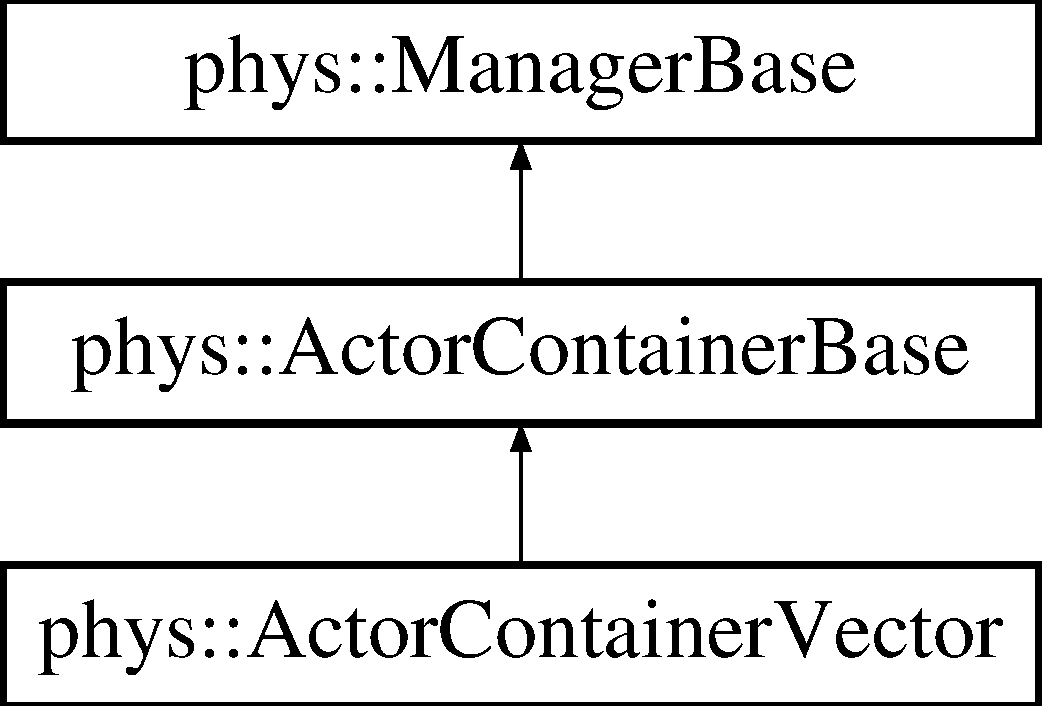
\includegraphics[height=2cm]{d3/d64/classphys_1_1ActorContainerVector}
\end{center}
\end{figure}
\subsection*{Public Member Functions}
\begin{DoxyCompactItemize}
\item 
\hyperlink{classphys_1_1ActorContainerVector_a65a17a06bc964c2b5f04a8dbb003622a}{ActorContainerVector} (\hyperlink{classphys_1_1World}{World} $\ast$Parent\_\-)
\begin{DoxyCompactList}\small\item\em Simple Constructor. \item\end{DoxyCompactList}\item 
virtual void \hyperlink{classphys_1_1ActorContainerVector_a4bc3e38f16caddee021a97739bebaf6e}{AddActor} (\hyperlink{classphys_1_1ActorBase}{ActorBase} $\ast$ActorToAdd)
\begin{DoxyCompactList}\small\item\em This will add an Actor to this container and the world. \item\end{DoxyCompactList}\item 
virtual \hyperlink{classphys_1_1ActorBase}{ActorBase} $\ast$ \hyperlink{classphys_1_1ActorContainerVector_a49e643bdeff78521de9c4a9fea59a0d2}{LastActorAdded} ()
\begin{DoxyCompactList}\small\item\em This provides an easy way to access the last Actor added to this container. \item\end{DoxyCompactList}\item 
virtual void \hyperlink{classphys_1_1ActorContainerVector_aeee5bd81601faed85e6a35f576c8d476}{RemoveActor} (\hyperlink{classphys_1_1ActorBase}{ActorBase} $\ast$ActorToRemove)
\begin{DoxyCompactList}\small\item\em Remove an Actor. \item\end{DoxyCompactList}\item 
virtual void \hyperlink{classphys_1_1ActorContainerVector_a430977daf010a25f53df6cf37954f8ca}{RemoveActorAtCursor} ()
\begin{DoxyCompactList}\small\item\em Removes the current actor. \item\end{DoxyCompactList}\item 
virtual \hyperlink{namespacephys_a460f6bc24c8dd347b05e0366ae34f34a}{Whole} \hyperlink{classphys_1_1ActorContainerVector_a6d2e5e68e23f5798ad10ba41e479d0f7}{GetActorCount} () const 
\begin{DoxyCompactList}\small\item\em Returns how many actors this stores. \item\end{DoxyCompactList}\item 
virtual void \hyperlink{classphys_1_1ActorContainerVector_ad9c2eb2a9405dcf687c86745afc9c031}{CursorToFirst} ()
\begin{DoxyCompactList}\small\item\em This moves the cursor to the first item in the container. \item\end{DoxyCompactList}\item 
virtual void \hyperlink{classphys_1_1ActorContainerVector_ac483bcdf348f55dc8b04a8805a002413}{CursorToPrevious} ()
\begin{DoxyCompactList}\small\item\em This moves the cursor to the previous item in the container. \item\end{DoxyCompactList}\item 
virtual void \hyperlink{classphys_1_1ActorContainerVector_a1c72366a6261d8e98dc0a9d2fad9f70f}{CursorToNext} ()
\begin{DoxyCompactList}\small\item\em This moves the cursor to the next item in the container. \item\end{DoxyCompactList}\item 
virtual void \hyperlink{classphys_1_1ActorContainerVector_aa6b08266bbb57a22c07ab50514e58db4}{CursorToLast} ()
\begin{DoxyCompactList}\small\item\em This moves the cursor to the last item in the container. \item\end{DoxyCompactList}\item 
virtual \hyperlink{classphys_1_1ActorBase}{ActorBase} $\ast$ \hyperlink{classphys_1_1ActorContainerVector_a280700490b368a963dd8feae044c7a6d}{GetAtCursor} () const 
\begin{DoxyCompactList}\small\item\em This gets the actor at the cursor. \item\end{DoxyCompactList}\item 
virtual \hyperlink{classphys_1_1ActorBase}{ActorBase} $\ast$ \hyperlink{classphys_1_1ActorContainerVector_a55ceecd017455f3185aa62798811e3c6}{GetFirst} () const 
\begin{DoxyCompactList}\small\item\em This gets the first actor in the container. \item\end{DoxyCompactList}\item 
virtual \hyperlink{classphys_1_1ActorBase}{ActorBase} $\ast$ \hyperlink{classphys_1_1ActorContainerVector_a211f6e419ef0b753cecf2c662a54511e}{GetLast} () const 
\begin{DoxyCompactList}\small\item\em This gets the last actor in the container. \item\end{DoxyCompactList}\item 
virtual \hyperlink{namespacephys_aa03900411993de7fbfec4789bc1d392e}{String} \hyperlink{classphys_1_1ActorContainerVector_a20d18213e69b3821ee973865df428e6d}{GetType} () const 
\begin{DoxyCompactList}\small\item\em Which kind of container it this anyway. \item\end{DoxyCompactList}\end{DoxyCompactItemize}
\subsection*{Public Attributes}
\begin{DoxyCompactItemize}
\item 
vector$<$ \hyperlink{classphys_1_1ActorBase}{ActorBase} $\ast$ $>$::iterator \hyperlink{classphys_1_1ActorContainerVector_a08bdad9b15e265b5d44470f21766b6ed}{cursor}
\begin{DoxyCompactList}\small\item\em This is used to store information about the cursor. \item\end{DoxyCompactList}\end{DoxyCompactItemize}


\subsection{Detailed Description}
A simple Actor Container using a vector. This inherits from std::vector and our \hyperlink{classphys_1_1ActorContainerBase}{phys::ActorContainerBase} to allow us to have access to a container through a standardized structure this way the phys::world doesn't need to worry about the details when accessing and storing actors 

Definition at line 57 of file actorcontainervector.h.



\subsection{Constructor \& Destructor Documentation}
\hypertarget{classphys_1_1ActorContainerVector_a65a17a06bc964c2b5f04a8dbb003622a}{
\index{phys::ActorContainerVector@{phys::ActorContainerVector}!ActorContainerVector@{ActorContainerVector}}
\index{ActorContainerVector@{ActorContainerVector}!phys::ActorContainerVector@{phys::ActorContainerVector}}
\subsubsection[{ActorContainerVector}]{\setlength{\rightskip}{0pt plus 5cm}phys::ActorContainerVector::ActorContainerVector ({\bf World} $\ast$ {\em Parent\_\-})}}
\label{d3/d64/classphys_1_1ActorContainerVector_a65a17a06bc964c2b5f04a8dbb003622a}


Simple Constructor. 

This creates and empty usable container based on std::vector. 
\begin{DoxyParams}{Parameters}
\item[{\em Parent\_\-}]this is a Pointer to the \hyperlink{classphys_1_1World}{phys::World} that will be using these actors. \end{DoxyParams}


Definition at line 45 of file actorcontainervector.cpp.



\subsection{Member Function Documentation}
\hypertarget{classphys_1_1ActorContainerVector_a4bc3e38f16caddee021a97739bebaf6e}{
\index{phys::ActorContainerVector@{phys::ActorContainerVector}!AddActor@{AddActor}}
\index{AddActor@{AddActor}!phys::ActorContainerVector@{phys::ActorContainerVector}}
\subsubsection[{AddActor}]{\setlength{\rightskip}{0pt plus 5cm}void phys::ActorContainerVector::AddActor ({\bf ActorBase} $\ast$ {\em ActorToAdd})\hspace{0.3cm}{\ttfamily  \mbox{[}virtual\mbox{]}}}}
\label{d3/d64/classphys_1_1ActorContainerVector_a4bc3e38f16caddee021a97739bebaf6e}


This will add an Actor to this container and the world. 

This will add an Actor to this container and the world, and handle the nitty gritty details of add this to physics subsystem and graphics subsystem. \par
\par
 This will not add the Actor to any specific location in the ordering of the container. 
\begin{DoxyParams}{Parameters}
\item[{\em ActorToAdd}]This is a pointer to the actor to add \end{DoxyParams}


Implements \hyperlink{classphys_1_1ActorContainerBase_a8dd213cba4915f68ac421fc9f341cbbe}{phys::ActorContainerBase}.



Definition at line 49 of file actorcontainervector.cpp.

\hypertarget{classphys_1_1ActorContainerVector_ad9c2eb2a9405dcf687c86745afc9c031}{
\index{phys::ActorContainerVector@{phys::ActorContainerVector}!CursorToFirst@{CursorToFirst}}
\index{CursorToFirst@{CursorToFirst}!phys::ActorContainerVector@{phys::ActorContainerVector}}
\subsubsection[{CursorToFirst}]{\setlength{\rightskip}{0pt plus 5cm}void phys::ActorContainerVector::CursorToFirst ()\hspace{0.3cm}{\ttfamily  \mbox{[}virtual\mbox{]}}}}
\label{d3/d64/classphys_1_1ActorContainerVector_ad9c2eb2a9405dcf687c86745afc9c031}


This moves the cursor to the first item in the container. 

This moves the cursor to the first item in the container change or return anything else. An exception will be throw if there are no valid items to move to with the cursor. There must be atleast one item to use any cursor moving functions. 

Implements \hyperlink{classphys_1_1ActorContainerBase_ab1a44758d7c17e70ff2e0f8de47424c3}{phys::ActorContainerBase}.



Definition at line 82 of file actorcontainervector.cpp.

\hypertarget{classphys_1_1ActorContainerVector_aa6b08266bbb57a22c07ab50514e58db4}{
\index{phys::ActorContainerVector@{phys::ActorContainerVector}!CursorToLast@{CursorToLast}}
\index{CursorToLast@{CursorToLast}!phys::ActorContainerVector@{phys::ActorContainerVector}}
\subsubsection[{CursorToLast}]{\setlength{\rightskip}{0pt plus 5cm}void phys::ActorContainerVector::CursorToLast ()\hspace{0.3cm}{\ttfamily  \mbox{[}virtual\mbox{]}}}}
\label{d3/d64/classphys_1_1ActorContainerVector_aa6b08266bbb57a22c07ab50514e58db4}


This moves the cursor to the last item in the container. 

This moves the cursor to the last item in the container change or return anything else. See \hyperlink{classphys_1_1ActorContainerVector_ad9c2eb2a9405dcf687c86745afc9c031}{CursorToFirst()} for more details. 

Implements \hyperlink{classphys_1_1ActorContainerBase_afad072e018a04c190e5e5fb93b82b354}{phys::ActorContainerBase}.



Definition at line 108 of file actorcontainervector.cpp.

\hypertarget{classphys_1_1ActorContainerVector_a1c72366a6261d8e98dc0a9d2fad9f70f}{
\index{phys::ActorContainerVector@{phys::ActorContainerVector}!CursorToNext@{CursorToNext}}
\index{CursorToNext@{CursorToNext}!phys::ActorContainerVector@{phys::ActorContainerVector}}
\subsubsection[{CursorToNext}]{\setlength{\rightskip}{0pt plus 5cm}void phys::ActorContainerVector::CursorToNext ()\hspace{0.3cm}{\ttfamily  \mbox{[}virtual\mbox{]}}}}
\label{d3/d64/classphys_1_1ActorContainerVector_a1c72366a6261d8e98dc0a9d2fad9f70f}


This moves the cursor to the next item in the container. 

This is the same as \hyperlink{classphys_1_1ActorContainerVector_ac483bcdf348f55dc8b04a8805a002413}{CursorToPrevious()} except if you start from the begin you'll work your way to the end. If you are at the end, you'll stay their if you call this again 

Implements \hyperlink{classphys_1_1ActorContainerBase_a1aa337456a4e74cb5740dbae08778072}{phys::ActorContainerBase}.



Definition at line 99 of file actorcontainervector.cpp.

\hypertarget{classphys_1_1ActorContainerVector_ac483bcdf348f55dc8b04a8805a002413}{
\index{phys::ActorContainerVector@{phys::ActorContainerVector}!CursorToPrevious@{CursorToPrevious}}
\index{CursorToPrevious@{CursorToPrevious}!phys::ActorContainerVector@{phys::ActorContainerVector}}
\subsubsection[{CursorToPrevious}]{\setlength{\rightskip}{0pt plus 5cm}void phys::ActorContainerVector::CursorToPrevious ()\hspace{0.3cm}{\ttfamily  \mbox{[}virtual\mbox{]}}}}
\label{d3/d64/classphys_1_1ActorContainerVector_ac483bcdf348f55dc8b04a8805a002413}


This moves the cursor to the previous item in the container. 

This moves the cursor to the previous item in the container, and if you started at the last item, you will visit every item in a properly implemented container, except for items that may have bee added during your traversal. It is also posible this could visit the same actor twice or more. When called from the first item this does nothing. An exception will be throw if there are no valid items to move to with the cursor. There must be atleast one item to use any cursor moving functions. 

Implements \hyperlink{classphys_1_1ActorContainerBase_a7c424168c0bbd973b283a083714123b3}{phys::ActorContainerBase}.



Definition at line 90 of file actorcontainervector.cpp.

\hypertarget{classphys_1_1ActorContainerVector_a6d2e5e68e23f5798ad10ba41e479d0f7}{
\index{phys::ActorContainerVector@{phys::ActorContainerVector}!GetActorCount@{GetActorCount}}
\index{GetActorCount@{GetActorCount}!phys::ActorContainerVector@{phys::ActorContainerVector}}
\subsubsection[{GetActorCount}]{\setlength{\rightskip}{0pt plus 5cm}{\bf Whole} phys::ActorContainerVector::GetActorCount () const\hspace{0.3cm}{\ttfamily  \mbox{[}virtual\mbox{]}}}}
\label{d3/d64/classphys_1_1ActorContainerVector_a6d2e5e68e23f5798ad10ba41e479d0f7}


Returns how many actors this stores. 

\begin{DoxyReturn}{Returns}
This returns a Whole number with the count of actors 
\end{DoxyReturn}


Implements \hyperlink{classphys_1_1ActorContainerBase_aa5ec651d4634b2d90efe2a76f9d2fbdd}{phys::ActorContainerBase}.



Definition at line 77 of file actorcontainervector.cpp.

\hypertarget{classphys_1_1ActorContainerVector_a280700490b368a963dd8feae044c7a6d}{
\index{phys::ActorContainerVector@{phys::ActorContainerVector}!GetAtCursor@{GetAtCursor}}
\index{GetAtCursor@{GetAtCursor}!phys::ActorContainerVector@{phys::ActorContainerVector}}
\subsubsection[{GetAtCursor}]{\setlength{\rightskip}{0pt plus 5cm}{\bf ActorBase} $\ast$ phys::ActorContainerVector::GetAtCursor () const\hspace{0.3cm}{\ttfamily  \mbox{[}virtual\mbox{]}}}}
\label{d3/d64/classphys_1_1ActorContainerVector_a280700490b368a963dd8feae044c7a6d}


This gets the actor at the cursor. 

This gets the actor at the cursor, and will not move the cursor. If the cursor has not be set to a location, any valid actor in the container could be returned. Will throw an exception when attempting to get from an empty container. \begin{DoxyReturn}{Returns}
This returns a pointer to an \hyperlink{classphys_1_1ActorBase}{ActorBase}. 
\end{DoxyReturn}


Implements \hyperlink{classphys_1_1ActorContainerBase_a2c8fb86a9e188aece105b2a753ccc19a}{phys::ActorContainerBase}.



Definition at line 116 of file actorcontainervector.cpp.

\hypertarget{classphys_1_1ActorContainerVector_a55ceecd017455f3185aa62798811e3c6}{
\index{phys::ActorContainerVector@{phys::ActorContainerVector}!GetFirst@{GetFirst}}
\index{GetFirst@{GetFirst}!phys::ActorContainerVector@{phys::ActorContainerVector}}
\subsubsection[{GetFirst}]{\setlength{\rightskip}{0pt plus 5cm}{\bf ActorBase} $\ast$ phys::ActorContainerVector::GetFirst () const\hspace{0.3cm}{\ttfamily  \mbox{[}virtual\mbox{]}}}}
\label{d3/d64/classphys_1_1ActorContainerVector_a55ceecd017455f3185aa62798811e3c6}


This gets the first actor in the container. 

This and the actor the cursor points at after \hyperlink{classphys_1_1ActorContainerVector_ad9c2eb2a9405dcf687c86745afc9c031}{CursorToFirst()} should match. \begin{DoxyReturn}{Returns}
This returns a pointer to an \hyperlink{classphys_1_1ActorBase}{ActorBase}. Will throw an exception when attempting to get from an empty container. 
\end{DoxyReturn}


Implements \hyperlink{classphys_1_1ActorContainerBase_ae703482d84a9c6726e28a8f26418b161}{phys::ActorContainerBase}.



Definition at line 124 of file actorcontainervector.cpp.

\hypertarget{classphys_1_1ActorContainerVector_a211f6e419ef0b753cecf2c662a54511e}{
\index{phys::ActorContainerVector@{phys::ActorContainerVector}!GetLast@{GetLast}}
\index{GetLast@{GetLast}!phys::ActorContainerVector@{phys::ActorContainerVector}}
\subsubsection[{GetLast}]{\setlength{\rightskip}{0pt plus 5cm}{\bf ActorBase} $\ast$ phys::ActorContainerVector::GetLast () const\hspace{0.3cm}{\ttfamily  \mbox{[}virtual\mbox{]}}}}
\label{d3/d64/classphys_1_1ActorContainerVector_a211f6e419ef0b753cecf2c662a54511e}


This gets the last actor in the container. 

This and the actor the cursor points at after \hyperlink{classphys_1_1ActorContainerVector_aa6b08266bbb57a22c07ab50514e58db4}{CursorToLast()} should match. \begin{DoxyReturn}{Returns}
This returns a pointer to an \hyperlink{classphys_1_1ActorBase}{ActorBase}. Will throw an exception when attempting to get from an empty container. 
\end{DoxyReturn}


Implements \hyperlink{classphys_1_1ActorContainerBase_a8efeffd5ae22085fe01af791b3ea559e}{phys::ActorContainerBase}.



Definition at line 129 of file actorcontainervector.cpp.

\hypertarget{classphys_1_1ActorContainerVector_a20d18213e69b3821ee973865df428e6d}{
\index{phys::ActorContainerVector@{phys::ActorContainerVector}!GetType@{GetType}}
\index{GetType@{GetType}!phys::ActorContainerVector@{phys::ActorContainerVector}}
\subsubsection[{GetType}]{\setlength{\rightskip}{0pt plus 5cm}{\bf String} phys::ActorContainerVector::GetType () const\hspace{0.3cm}{\ttfamily  \mbox{[}virtual\mbox{]}}}}
\label{d3/d64/classphys_1_1ActorContainerVector_a20d18213e69b3821ee973865df428e6d}


Which kind of container it this anyway. 

Since this interface could be used with any type of containers and innumerable 3rd party container implemention this can be used to more safely cast this container to a more specific type. \begin{DoxyReturn}{Returns}
This returns a \hyperlink{namespacephys_aa03900411993de7fbfec4789bc1d392e}{phys::String} 
\end{DoxyReturn}


Implements \hyperlink{classphys_1_1ActorContainerBase_a526dab176597858680490d128d0584a3}{phys::ActorContainerBase}.



Definition at line 134 of file actorcontainervector.cpp.

\hypertarget{classphys_1_1ActorContainerVector_a49e643bdeff78521de9c4a9fea59a0d2}{
\index{phys::ActorContainerVector@{phys::ActorContainerVector}!LastActorAdded@{LastActorAdded}}
\index{LastActorAdded@{LastActorAdded}!phys::ActorContainerVector@{phys::ActorContainerVector}}
\subsubsection[{LastActorAdded}]{\setlength{\rightskip}{0pt plus 5cm}{\bf ActorBase} $\ast$ phys::ActorContainerVector::LastActorAdded ()\hspace{0.3cm}{\ttfamily  \mbox{[}virtual\mbox{]}}}}
\label{d3/d64/classphys_1_1ActorContainerVector_a49e643bdeff78521de9c4a9fea59a0d2}


This provides an easy way to access the last Actor added to this container. 

For many containers this will simply return a pointer to the last actorl 

Implements \hyperlink{classphys_1_1ActorContainerBase_a6ccc6d058bcbbe0b9a638e28fb136477}{phys::ActorContainerBase}.



Definition at line 55 of file actorcontainervector.cpp.

\hypertarget{classphys_1_1ActorContainerVector_aeee5bd81601faed85e6a35f576c8d476}{
\index{phys::ActorContainerVector@{phys::ActorContainerVector}!RemoveActor@{RemoveActor}}
\index{RemoveActor@{RemoveActor}!phys::ActorContainerVector@{phys::ActorContainerVector}}
\subsubsection[{RemoveActor}]{\setlength{\rightskip}{0pt plus 5cm}void phys::ActorContainerVector::RemoveActor ({\bf ActorBase} $\ast$ {\em ActorToRemove})\hspace{0.3cm}{\ttfamily  \mbox{[}virtual\mbox{]}}}}
\label{d3/d64/classphys_1_1ActorContainerVector_aeee5bd81601faed85e6a35f576c8d476}


Remove an Actor. 

Remove all references of the actor pointed from the container. Will throw an exception when attempting to remove and no match could be found. 

Implements \hyperlink{classphys_1_1ActorContainerBase_a523072e42f6b581d044432f84a84ede4}{phys::ActorContainerBase}.



Definition at line 60 of file actorcontainervector.cpp.

\hypertarget{classphys_1_1ActorContainerVector_a430977daf010a25f53df6cf37954f8ca}{
\index{phys::ActorContainerVector@{phys::ActorContainerVector}!RemoveActorAtCursor@{RemoveActorAtCursor}}
\index{RemoveActorAtCursor@{RemoveActorAtCursor}!phys::ActorContainerVector@{phys::ActorContainerVector}}
\subsubsection[{RemoveActorAtCursor}]{\setlength{\rightskip}{0pt plus 5cm}void phys::ActorContainerVector::RemoveActorAtCursor ()\hspace{0.3cm}{\ttfamily  \mbox{[}virtual\mbox{]}}}}
\label{d3/d64/classphys_1_1ActorContainerVector_a430977daf010a25f53df6cf37954f8ca}


Removes the current actor. 

This removes the actor the cursor at. Will throw an exception when attempting to remove from an empty container. Where the cursor goes is implementation dependent. 

Implements \hyperlink{classphys_1_1ActorContainerBase_a60f37a056e8750f3b389c5ceed14520c}{phys::ActorContainerBase}.



Definition at line 72 of file actorcontainervector.cpp.



\subsection{Member Data Documentation}
\hypertarget{classphys_1_1ActorContainerVector_a08bdad9b15e265b5d44470f21766b6ed}{
\index{phys::ActorContainerVector@{phys::ActorContainerVector}!cursor@{cursor}}
\index{cursor@{cursor}!phys::ActorContainerVector@{phys::ActorContainerVector}}
\subsubsection[{cursor}]{\setlength{\rightskip}{0pt plus 5cm}vector$<${\bf ActorBase}$\ast$$>$::iterator {\bf phys::ActorContainerVector::cursor}}}
\label{d3/d64/classphys_1_1ActorContainerVector_a08bdad9b15e265b5d44470f21766b6ed}


This is used to store information about the cursor. 

This implementation of \hyperlink{classphys_1_1ActorContainerBase}{ActorContainerBase} will use this, and only this to access the cursor so feel free to use this instead. 

Definition at line 94 of file actorcontainervector.h.



The documentation for this class was generated from the following files:\begin{DoxyCompactItemize}
\item 
actorcontainervector.h\item 
actorcontainervector.cpp\end{DoxyCompactItemize}

\hypertarget{classphys_1_1ActorRigid}{
\section{phys::ActorRigid Class Reference}
\label{d8/d71/classphys_1_1ActorRigid}\index{phys::ActorRigid@{phys::ActorRigid}}
}


This is the actor class for Rigid Objects.  




{\ttfamily \#include $<$actorbase.h$>$}

Inheritance diagram for phys::ActorRigid:\begin{figure}[H]
\begin{center}
\leavevmode
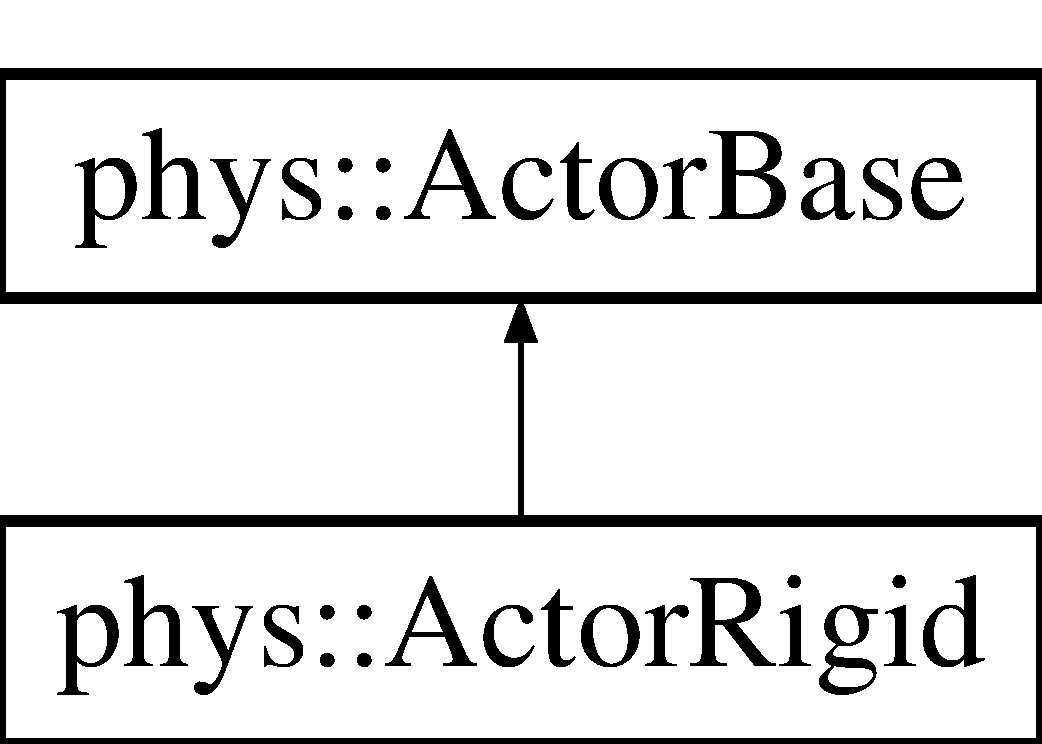
\includegraphics[height=2cm]{d8/d71/classphys_1_1ActorRigid}
\end{center}
\end{figure}
\subsection*{Public Member Functions}
\begin{DoxyCompactItemize}
\item 
\hyperlink{classphys_1_1ActorRigid_ac42c05745d57eb5745de3f34e820b72d}{ActorRigid} (\hyperlink{namespacephys_af7eb897198d265b8e868f45240230d5f}{Real} mass, \hyperlink{namespacephys_aa03900411993de7fbfec4789bc1d392e}{String} name, \hyperlink{namespacephys_aa03900411993de7fbfec4789bc1d392e}{String} file, \hyperlink{namespacephys_aa03900411993de7fbfec4789bc1d392e}{String} group, \hyperlink{classphys_1_1World}{World} $\ast$\_\-World)
\begin{DoxyCompactList}\small\item\em Descriptive constructor. \item\end{DoxyCompactList}\item 
virtual \hyperlink{classphys_1_1ActorRigid_ab317b5a2578157e54655a1aea8f4d058}{$\sim$ActorRigid} ()
\begin{DoxyCompactList}\small\item\em Destructor. \item\end{DoxyCompactList}\item 
void \hyperlink{classphys_1_1ActorRigid_aab4a408ce0724be6adf4c9f51f55f8a1}{CreateShapeFromMeshDynamic} (short unsigned int accuracy=1)
\begin{DoxyCompactList}\small\item\em Creates a collision shape from mesh file. \item\end{DoxyCompactList}\item 
void \hyperlink{classphys_1_1ActorRigid_a84554dcaaf2475ba0ec7dcb9235050ac}{CreateShapeFromMeshStatic} ()
\begin{DoxyCompactList}\small\item\em Creates a collision shape from mesh file. \item\end{DoxyCompactList}\item 
void \hyperlink{classphys_1_1ActorRigid_adaed962ee8ed788612e541fb00867c78}{LimitMovementOnAxis} (bool x, bool y, bool z)
\begin{DoxyCompactList}\small\item\em Restricts movement on the axis or axies of your choice. \item\end{DoxyCompactList}\end{DoxyCompactItemize}
\subsection*{Protected Member Functions}
\begin{DoxyCompactItemize}
\item 
void \hyperlink{classphys_1_1ActorRigid_a19227c52b972cd96ad69a7b6273e2bbf}{CreateRigidObject} (\hyperlink{namespacephys_af7eb897198d265b8e868f45240230d5f}{Real} pmass)
\begin{DoxyCompactList}\small\item\em Creates a rigid object for the actor. \item\end{DoxyCompactList}\item 
void \hyperlink{classphys_1_1ActorRigid_a3c56eb06fe6a7d468b7a67c45ade7be4}{AddObjectToWorld} (\hyperlink{classphys_1_1World}{World} $\ast$TargetWorld, btSoftRigidDynamicsWorld $\ast$btWorld)
\begin{DoxyCompactList}\small\item\em Adds the actor to the physics world. \item\end{DoxyCompactList}\end{DoxyCompactItemize}
\subsection*{Protected Attributes}
\begin{DoxyCompactItemize}
\item 
\hypertarget{classphys_1_1ActorRigid_a690889f942e177644f4f8521f509c88d}{
btRigidBody $\ast$ \hyperlink{classphys_1_1ActorRigid_a690889f942e177644f4f8521f509c88d}{physrigidbody}}
\label{d8/d71/classphys_1_1ActorRigid_a690889f942e177644f4f8521f509c88d}

\begin{DoxyCompactList}\small\item\em Used to simulate the behavior of a btRigidBody. \item\end{DoxyCompactList}\end{DoxyCompactItemize}


\subsection{Detailed Description}
This is the actor class for Rigid Objects. This class should be used to make any rigid object that can be moved as a result of force. Most objects will fall into this catagory. A few examples of a Rigid Object: Boxes, Car Frames, Chairs, etc. For Semi Rigid bodies that are deformable, like jello, it is better to use \hyperlink{classphys_1_1ActorSoft}{ActorSoft}. 

Definition at line 87 of file actorrigid.h.



\subsection{Constructor \& Destructor Documentation}
\hypertarget{classphys_1_1ActorRigid_ac42c05745d57eb5745de3f34e820b72d}{
\index{phys::ActorRigid@{phys::ActorRigid}!ActorRigid@{ActorRigid}}
\index{ActorRigid@{ActorRigid}!phys::ActorRigid@{phys::ActorRigid}}
\subsubsection[{ActorRigid}]{\setlength{\rightskip}{0pt plus 5cm}phys::ActorRigid::ActorRigid ({\bf Real} {\em mass}, \/  {\bf String} {\em name}, \/  {\bf String} {\em file}, \/  {\bf String} {\em group}, \/  {\bf World} $\ast$ {\em \_\-World})}}
\label{d8/d71/classphys_1_1ActorRigid_ac42c05745d57eb5745de3f34e820b72d}


Descriptive constructor. 

This constructor contains the basic information needed to make a Rigid Object. \par
 This class inherits from \hyperlink{classphys_1_1ActorBase}{ActorBase}. 
\begin{DoxyParams}{Parameters}
\item[{\em mass}]The mass the object will have in the \hyperlink{classphys_1_1World}{World}. \item[{\em name}]The name of the actor. \item[{\em file}]The 3d mesh file that contains the 3d model the actor will use. \item[{\em group}]The resource group where the 3d mesh and other related files can be found. \item[{\em \_\-World}]Pointer to the \hyperlink{classphys_1_1World}{World} this object will be added to. \end{DoxyParams}


Definition at line 53 of file actorrigid.cpp.

\hypertarget{classphys_1_1ActorRigid_ab317b5a2578157e54655a1aea8f4d058}{
\index{phys::ActorRigid@{phys::ActorRigid}!$\sim$ActorRigid@{$\sim$ActorRigid}}
\index{$\sim$ActorRigid@{$\sim$ActorRigid}!phys::ActorRigid@{phys::ActorRigid}}
\subsubsection[{$\sim$ActorRigid}]{\setlength{\rightskip}{0pt plus 5cm}phys::ActorRigid::$\sim$ActorRigid ()\hspace{0.3cm}{\ttfamily  \mbox{[}virtual\mbox{]}}}}
\label{d8/d71/classphys_1_1ActorRigid_ab317b5a2578157e54655a1aea8f4d058}


Destructor. 

The class destructor. 

Definition at line 58 of file actorrigid.cpp.



\subsection{Member Function Documentation}
\hypertarget{classphys_1_1ActorRigid_a3c56eb06fe6a7d468b7a67c45ade7be4}{
\index{phys::ActorRigid@{phys::ActorRigid}!AddObjectToWorld@{AddObjectToWorld}}
\index{AddObjectToWorld@{AddObjectToWorld}!phys::ActorRigid@{phys::ActorRigid}}
\subsubsection[{AddObjectToWorld}]{\setlength{\rightskip}{0pt plus 5cm}void phys::ActorRigid::AddObjectToWorld ({\bf World} $\ast$ {\em TargetWorld}, \/  btSoftRigidDynamicsWorld $\ast$ {\em btWorld})\hspace{0.3cm}{\ttfamily  \mbox{[}protected, virtual\mbox{]}}}}
\label{d8/d71/classphys_1_1ActorRigid_a3c56eb06fe6a7d468b7a67c45ade7be4}


Adds the actor to the physics world. 

Adds the actor to the physics world. \par
 This is automaticly called by the PhysWorlds AddActor function and shouldn't be called manually. 
\begin{DoxyParams}{Parameters}
\item[{\em TargetWorld}]Pointer to the \hyperlink{classphys_1_1World}{World} class. \item[{\em btWorld}]Pointer to the physics world. \end{DoxyParams}


Implements \hyperlink{classphys_1_1ActorBase_ac5d4ad5a634b16000742f506ed5957fb}{phys::ActorBase}.



Definition at line 70 of file actorrigid.cpp.

\hypertarget{classphys_1_1ActorRigid_a19227c52b972cd96ad69a7b6273e2bbf}{
\index{phys::ActorRigid@{phys::ActorRigid}!CreateRigidObject@{CreateRigidObject}}
\index{CreateRigidObject@{CreateRigidObject}!phys::ActorRigid@{phys::ActorRigid}}
\subsubsection[{CreateRigidObject}]{\setlength{\rightskip}{0pt plus 5cm}void phys::ActorRigid::CreateRigidObject ({\bf Real} {\em pmass})\hspace{0.3cm}{\ttfamily  \mbox{[}protected\mbox{]}}}}
\label{d8/d71/classphys_1_1ActorRigid_a19227c52b972cd96ad69a7b6273e2bbf}


Creates a rigid object for the actor. 

Creates a rigid object to be placed in the physics world later. \par
 This is automaticly called by the Constructor and shouldn't be called manually. 
\begin{DoxyParams}{Parameters}
\item[{\em pmass}]\char`\"{}Real Mass\char`\"{} The mass of the object. \end{DoxyParams}


Definition at line 63 of file actorrigid.cpp.

\hypertarget{classphys_1_1ActorRigid_aab4a408ce0724be6adf4c9f51f55f8a1}{
\index{phys::ActorRigid@{phys::ActorRigid}!CreateShapeFromMeshDynamic@{CreateShapeFromMeshDynamic}}
\index{CreateShapeFromMeshDynamic@{CreateShapeFromMeshDynamic}!phys::ActorRigid@{phys::ActorRigid}}
\subsubsection[{CreateShapeFromMeshDynamic}]{\setlength{\rightskip}{0pt plus 5cm}void phys::ActorRigid::CreateShapeFromMeshDynamic (short unsigned int {\em accuracy} = {\ttfamily 1})\hspace{0.3cm}{\ttfamily  \mbox{[}virtual\mbox{]}}}}
\label{d8/d71/classphys_1_1ActorRigid_aab4a408ce0724be6adf4c9f51f55f8a1}


Creates a collision shape from mesh file. 

This function will read the location of every verticy in the mesh file and use that to construct a triangle mesh shape and attach it to this objects collision shape. This shoiuld be used with only with Dynamic objects. 
\begin{DoxyParams}{Parameters}
\item[{\em accuracy}]A value from 1 to 4. The higher the more accurate, but the more resource intensive \end{DoxyParams}


\begin{Desc}
\item[\hyperlink{todo__todo000001}{Todo}]
\begin{DoxyItemize}
\item Check for thread safety 
\end{DoxyItemize}\end{Desc}


\begin{Desc}
\item[\hyperlink{todo__todo000002}{Todo}]add code here to increase the verticies that is used to create the hull from the first accuracy setting. \end{Desc}


\begin{Desc}
\item[\hyperlink{todo__todo000003}{Todo}]add code here for compound shapes of convex hulls \end{Desc}




Implements \hyperlink{classphys_1_1ActorBase_aa41370f6d2031a9dad8df45bd7f3bcc6}{phys::ActorBase}.



Definition at line 76 of file actorrigid.cpp.

\hypertarget{classphys_1_1ActorRigid_a84554dcaaf2475ba0ec7dcb9235050ac}{
\index{phys::ActorRigid@{phys::ActorRigid}!CreateShapeFromMeshStatic@{CreateShapeFromMeshStatic}}
\index{CreateShapeFromMeshStatic@{CreateShapeFromMeshStatic}!phys::ActorRigid@{phys::ActorRigid}}
\subsubsection[{CreateShapeFromMeshStatic}]{\setlength{\rightskip}{0pt plus 5cm}void phys::ActorRigid::CreateShapeFromMeshStatic ()}}
\label{d8/d71/classphys_1_1ActorRigid_a84554dcaaf2475ba0ec7dcb9235050ac}


Creates a collision shape from mesh file. 

This function will read the location of every verticy in the mesh file and use that to construct a triangle mesh shape and attach it to this objects collision shape. This shoiuld be used with only with Dynamic objects. 

\begin{Desc}
\item[\hyperlink{todo__todo000004}{Todo}]
\begin{DoxyItemize}
\item Check for thread safety 
\end{DoxyItemize}\end{Desc}




Definition at line 139 of file actorrigid.cpp.

\hypertarget{classphys_1_1ActorRigid_adaed962ee8ed788612e541fb00867c78}{
\index{phys::ActorRigid@{phys::ActorRigid}!LimitMovementOnAxis@{LimitMovementOnAxis}}
\index{LimitMovementOnAxis@{LimitMovementOnAxis}!phys::ActorRigid@{phys::ActorRigid}}
\subsubsection[{LimitMovementOnAxis}]{\setlength{\rightskip}{0pt plus 5cm}void phys::ActorRigid::LimitMovementOnAxis (bool {\em x}, \/  bool {\em y}, \/  bool {\em z})}}
\label{d8/d71/classphys_1_1ActorRigid_adaed962ee8ed788612e541fb00867c78}


Restricts movement on the axis or axies of your choice. 

This function will lock any and all axies you define you want to be locked. Simply pass true to allow movement on that axis, false if you don't. This function is primarily useful for 2D games, in which if you are viewing the playing area from the side you can pass in LimitMovementOnAxis(true,true,false) and the object will only be able to move up, down, or side to side, but not in or out. 
\begin{DoxyParams}{Parameters}
\item[{\em x}]Allow or Disallow use of the X axis for movement. \item[{\em y}]Allow or Disallow use of the Y axis for movement. \item[{\em z}]Allow or Disallow use of the Z axis for movement. \end{DoxyParams}


Definition at line 150 of file actorrigid.cpp.



The documentation for this class was generated from the following files:\begin{DoxyCompactItemize}
\item 
actorrigid.h\item 
actorrigid.cpp\end{DoxyCompactItemize}

\hypertarget{classphys_1_1ActorSoft}{
\section{phys::ActorSoft Class Reference}
\label{d4/d23/classphys_1_1ActorSoft}\index{phys::ActorSoft@{phys::ActorSoft}}
}


This is the actor class for Soft Objects.  




{\ttfamily \#include $<$physactor.h$>$}

Inheritance diagram for phys::ActorSoft:\begin{figure}[H]
\begin{center}
\leavevmode
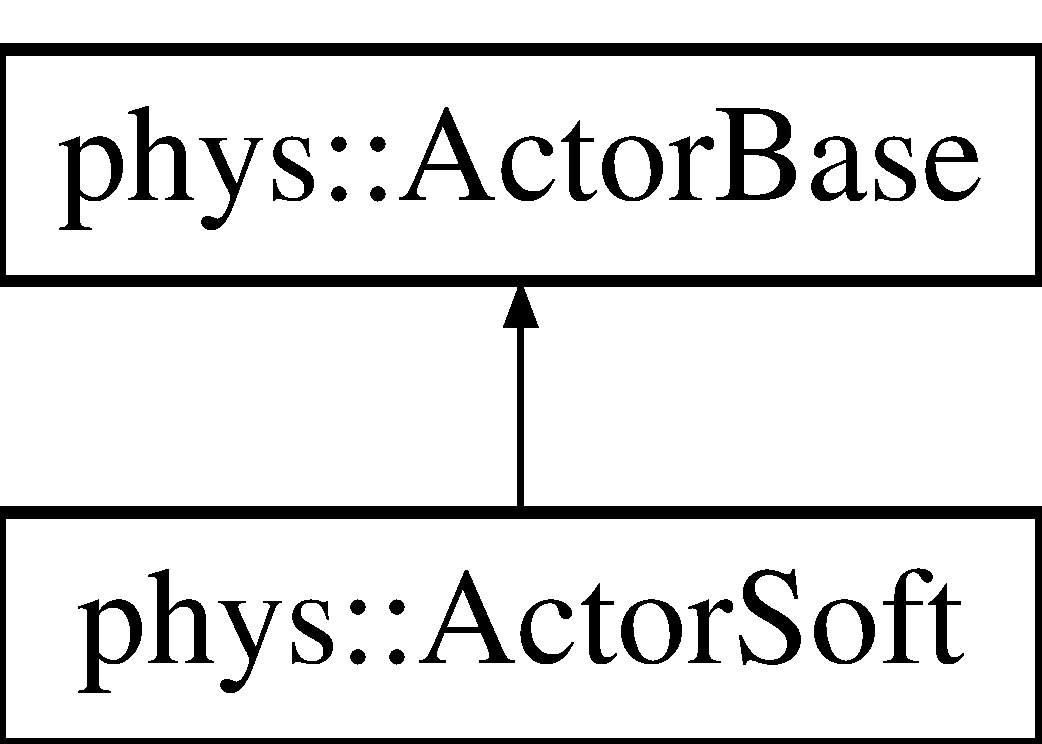
\includegraphics[height=2cm]{d4/d23/classphys_1_1ActorSoft}
\end{center}
\end{figure}
\subsection*{Public Member Functions}
\begin{DoxyCompactItemize}
\item 
virtual \hyperlink{classphys_1_1ActorSoft_a636c145f1e468fd45adc8da2a1708fbe}{$\sim$ActorSoft} ()
\begin{DoxyCompactList}\small\item\em Destructor. \item\end{DoxyCompactList}\item 
void \hyperlink{classphys_1_1ActorSoft_a51d78e0f503c3c815511c3d246b426ae}{CreateShapeFromMesh} ()
\begin{DoxyCompactList}\small\item\em Creates a collision shape from mesh file. \item\end{DoxyCompactList}\end{DoxyCompactItemize}
\subsection*{Protected Member Functions}
\begin{DoxyCompactItemize}
\item 
void \hyperlink{classphys_1_1ActorSoft_a04c98bb0ab9ed7c1dfc3435d49403ef4}{CreateSoftObject} (btSoftBodyWorldInfo $\ast$softworldinfo, int nodecount, btVector3 $\ast$nodearray, btScalar $\ast$massarray)
\begin{DoxyCompactList}\small\item\em Creates a soft object for the actor. \item\end{DoxyCompactList}\item 
void \hyperlink{classphys_1_1ActorSoft_a3a704ab32f847a5d0e060f8a592efefd}{AddObjectToWorld} (\hyperlink{classphys_1_1World}{World} $\ast$TargetWorld, btSoftRigidDynamicsWorld $\ast$btWorld)
\begin{DoxyCompactList}\small\item\em Adds the actor to the physics world. \item\end{DoxyCompactList}\end{DoxyCompactItemize}
\subsection*{Protected Attributes}
\begin{DoxyCompactItemize}
\item 
\hypertarget{classphys_1_1ActorSoft_ab3b2c8e1f94dff3e3244a5024595afef}{
btSoftBody $\ast$ \hyperlink{classphys_1_1ActorSoft_ab3b2c8e1f94dff3e3244a5024595afef}{physsoftbody}}
\label{d4/d23/classphys_1_1ActorSoft_ab3b2c8e1f94dff3e3244a5024595afef}

\begin{DoxyCompactList}\small\item\em Used to simulate the functionality of a btSoftBody for use with the physics subsystem. \item\end{DoxyCompactList}\end{DoxyCompactItemize}


\subsection{Detailed Description}
This is the actor class for Soft Objects. This class should be used to make any soft object that, like \hyperlink{classphys_1_1ActorRigid}{ActorRigid}, can be moved or manipulated as a result of force. Examples of soft objects are: Paper, Rope, and Cloth. Semi Rigid bodies that are still somewhat deformable, like Jello, should be made as a soft object. 

Definition at line 310 of file physactor.h.



\subsection{Constructor \& Destructor Documentation}
\hypertarget{classphys_1_1ActorSoft_a636c145f1e468fd45adc8da2a1708fbe}{
\index{phys::ActorSoft@{phys::ActorSoft}!$\sim$ActorSoft@{$\sim$ActorSoft}}
\index{$\sim$ActorSoft@{$\sim$ActorSoft}!phys::ActorSoft@{phys::ActorSoft}}
\subsubsection[{$\sim$ActorSoft}]{\setlength{\rightskip}{0pt plus 5cm}phys::ActorSoft::$\sim$ActorSoft ()\hspace{0.3cm}{\ttfamily  \mbox{[}virtual\mbox{]}}}}
\label{d4/d23/classphys_1_1ActorSoft_a636c145f1e468fd45adc8da2a1708fbe}


Destructor. 

The class destructor. 

Definition at line 458 of file physactor.cpp.



\subsection{Member Function Documentation}
\hypertarget{classphys_1_1ActorSoft_a3a704ab32f847a5d0e060f8a592efefd}{
\index{phys::ActorSoft@{phys::ActorSoft}!AddObjectToWorld@{AddObjectToWorld}}
\index{AddObjectToWorld@{AddObjectToWorld}!phys::ActorSoft@{phys::ActorSoft}}
\subsubsection[{AddObjectToWorld}]{\setlength{\rightskip}{0pt plus 5cm}void phys::ActorSoft::AddObjectToWorld ({\bf World} $\ast$ {\em TargetWorld}, \/  btSoftRigidDynamicsWorld $\ast$ {\em btWorld})\hspace{0.3cm}{\ttfamily  \mbox{[}protected, virtual\mbox{]}}}}
\label{d4/d23/classphys_1_1ActorSoft_a3a704ab32f847a5d0e060f8a592efefd}


Adds the actor to the physics world. 

Adds the actor to the physics world. \par
 This is automaticly called by the PhysWorlds AddActor function and shouldn't be called manually. 
\begin{DoxyParams}{Parameters}
\item[{\em TargetWorld}]Pointer to the \hyperlink{classphys_1_1World}{World} class. \item[{\em btWorld}]Pointer to the physics world. \end{DoxyParams}


Implements \hyperlink{classphys_1_1ActorBase_ac5d4ad5a634b16000742f506ed5957fb}{phys::ActorBase}.



Definition at line 469 of file physactor.cpp.

\hypertarget{classphys_1_1ActorSoft_a51d78e0f503c3c815511c3d246b426ae}{
\index{phys::ActorSoft@{phys::ActorSoft}!CreateShapeFromMesh@{CreateShapeFromMesh}}
\index{CreateShapeFromMesh@{CreateShapeFromMesh}!phys::ActorSoft@{phys::ActorSoft}}
\subsubsection[{CreateShapeFromMesh}]{\setlength{\rightskip}{0pt plus 5cm}void phys::ActorSoft::CreateShapeFromMesh ()}}
\label{d4/d23/classphys_1_1ActorSoft_a51d78e0f503c3c815511c3d246b426ae}


Creates a collision shape from mesh file. 

This function will read the location of every verticy in the mesh file and use that to construct a triangle mesh shape and attach it to this objects collision shape. 

Definition at line 474 of file physactor.cpp.

\hypertarget{classphys_1_1ActorSoft_a04c98bb0ab9ed7c1dfc3435d49403ef4}{
\index{phys::ActorSoft@{phys::ActorSoft}!CreateSoftObject@{CreateSoftObject}}
\index{CreateSoftObject@{CreateSoftObject}!phys::ActorSoft@{phys::ActorSoft}}
\subsubsection[{CreateSoftObject}]{\setlength{\rightskip}{0pt plus 5cm}void phys::ActorSoft::CreateSoftObject (btSoftBodyWorldInfo $\ast$ {\em softworldinfo}, \/  int {\em nodecount}, \/  btVector3 $\ast$ {\em nodearray}, \/  btScalar $\ast$ {\em massarray})\hspace{0.3cm}{\ttfamily  \mbox{[}protected\mbox{]}}}}
\label{d4/d23/classphys_1_1ActorSoft_a04c98bb0ab9ed7c1dfc3435d49403ef4}


Creates a soft object for the actor. 

Creates a soft object to be placed in the physics world later. \par
 This is automaticly called by the Constructor and shouldn't be called manually. 
\begin{DoxyParams}{Parameters}
\item[{\em softworldinfo}]Currently Unused \item[{\em nodecount}]Currently Unused \item[{\em nodearray}]Currently Unused \item[{\em massarray}]Currently Unused \end{DoxyParams}


Definition at line 463 of file physactor.cpp.



The documentation for this class was generated from the following files:\begin{DoxyCompactItemize}
\item 
physactor.h\item 
physactor.cpp\end{DoxyCompactItemize}

\hypertarget{classphys_1_1ActorTerrain}{
\subsection{phys::ActorTerrain Class Reference}
\label{classphys_1_1ActorTerrain}\index{phys::ActorTerrain@{phys::ActorTerrain}}
}


This is actor class for terrain.  




{\ttfamily \#include $<$actorterrain.h$>$}

Inheritance diagram for phys::ActorTerrain:\begin{figure}[H]
\begin{center}
\leavevmode
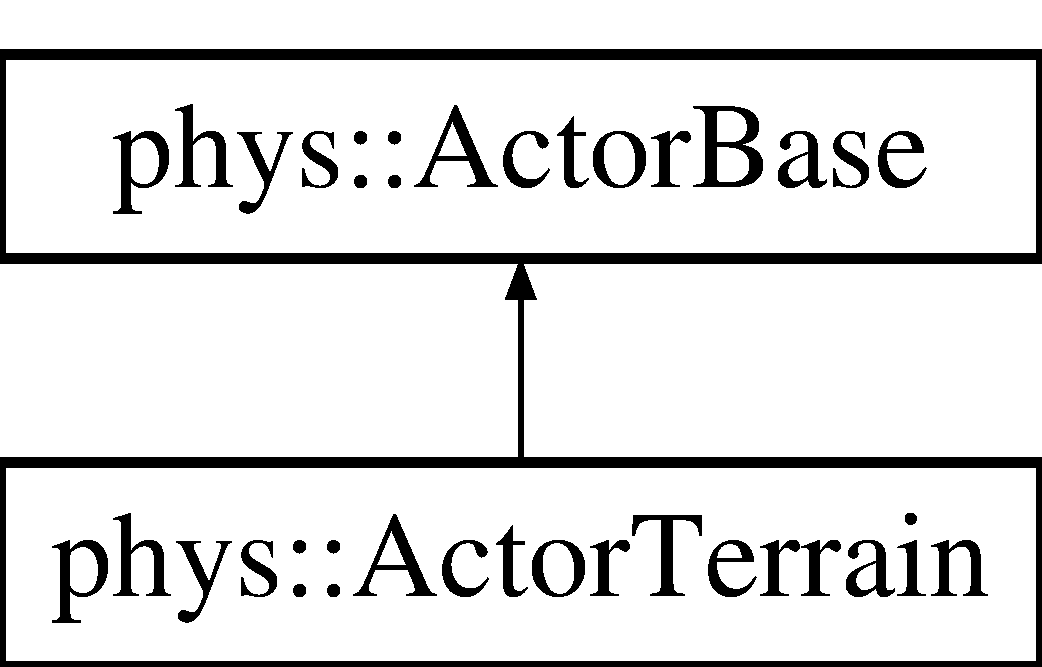
\includegraphics[height=2.000000cm]{classphys_1_1ActorTerrain}
\end{center}
\end{figure}
\subsubsection*{Public Member Functions}
\begin{DoxyCompactItemize}
\item 
\hyperlink{classphys_1_1ActorTerrain_af0d3b88d5ee409c5451bb13a20254176}{ActorTerrain} (\hyperlink{classphys_1_1Vector3}{Vector3} InitPosition, \hyperlink{namespacephys_aa03900411993de7fbfec4789bc1d392e}{String} name, \hyperlink{namespacephys_aa03900411993de7fbfec4789bc1d392e}{String} file, \hyperlink{namespacephys_aa03900411993de7fbfec4789bc1d392e}{String} group)
\begin{DoxyCompactList}\small\item\em Class constructor. \item\end{DoxyCompactList}\item 
\hyperlink{classphys_1_1ActorTerrain_af6ef2e3694b7afe0b59cfa0909c0490c}{$\sim$ActorTerrain} ()
\begin{DoxyCompactList}\small\item\em Class destructor. \item\end{DoxyCompactList}\item 
void \hyperlink{classphys_1_1ActorTerrain_aaed245d7af66230aaabb02a84e891bb0}{CreateShapeFromMeshStatic} (bool UseAllSubmeshes=false)
\begin{DoxyCompactList}\small\item\em Creates a collision shape from mesh file. \item\end{DoxyCompactList}\item 
void \hyperlink{classphys_1_1ActorTerrain_a9fed38501411c0cf7a1e9f4f36af6ac7}{CreateShapeFromMeshDynamic} (short unsigned int Accuracy, bool UseAllSubmeshes=false)
\begin{DoxyCompactList}\small\item\em Compatability function. \item\end{DoxyCompactList}\item 
virtual bool \hyperlink{classphys_1_1ActorTerrain_a37d0fb3d028ac1946e3553f7f0eef56d}{IsStaticOrKinematic} ()
\begin{DoxyCompactList}\small\item\em Checks of the actor is static or kinematic. \item\end{DoxyCompactList}\item 
std::string \hyperlink{classphys_1_1ActorTerrain_a08f306ae189e55d780dcaa2c43d7b6eb}{GetName} () const 
\begin{DoxyCompactList}\small\item\em Retrieves the name of the object. \item\end{DoxyCompactList}\item 
virtual \hyperlink{classphys_1_1ActorRigidPhysicsSettings}{ActorRigidPhysicsSettings} $\ast$ \hyperlink{classphys_1_1ActorTerrain_a4210cd05b0ec97f089fc6420e4b0bae8}{GetPhysicsSettings} ()
\begin{DoxyCompactList}\small\item\em Gets the physics settings class associated with this actor. \item\end{DoxyCompactList}\item 
virtual void \hyperlink{classphys_1_1ActorTerrain_a890ee6f67fda30381bce9c949ae36566}{AddObjectToWorld} (\hyperlink{classphys_1_1World}{World} $\ast$TargetWorld)
\begin{DoxyCompactList}\small\item\em Adds the actor to the physics world. \item\end{DoxyCompactList}\item 
virtual void \hyperlink{classphys_1_1ActorTerrain_aeded1fdabfc4dd407f81fcc5b97c1f77}{RemoveObjectFromWorld} (\hyperlink{classphys_1_1World}{World} $\ast$TargetWorld)
\begin{DoxyCompactList}\small\item\em Removes the actor from the physics world. \item\end{DoxyCompactList}\item 
virtual btRigidBody $\ast$ \hyperlink{classphys_1_1ActorTerrain_a1bed32f1b9afd1bd28c231b7505c267e}{GetBulletObject} ()
\begin{DoxyCompactList}\small\item\em Get the Physics data raw from the physic subsystem. \item\end{DoxyCompactList}\end{DoxyCompactItemize}
\subsubsection*{Protected Member Functions}
\begin{DoxyCompactItemize}
\item 
\hypertarget{classphys_1_1ActorTerrain_ade758919c0f2b58ad1fe4bfd388d79af}{
void \hyperlink{classphys_1_1ActorTerrain_ade758919c0f2b58ad1fe4bfd388d79af}{CreateCollisionTerrain} ()}
\label{classphys_1_1ActorTerrain_ade758919c0f2b58ad1fe4bfd388d79af}

\begin{DoxyCompactList}\small\item\em Uses value already passed into this to create the physics shapes. \item\end{DoxyCompactList}\end{DoxyCompactItemize}
\subsubsection*{Protected Attributes}
\begin{DoxyCompactItemize}
\item 
\hypertarget{classphys_1_1ActorTerrain_a86b22aad61a7ffceb5c757ddcbca48c3}{
btRigidBody $\ast$ \hyperlink{classphys_1_1ActorTerrain_a86b22aad61a7ffceb5c757ddcbca48c3}{RigidBody}}
\label{classphys_1_1ActorTerrain_a86b22aad61a7ffceb5c757ddcbca48c3}

\begin{DoxyCompactList}\small\item\em The physics data. \item\end{DoxyCompactList}\end{DoxyCompactItemize}


\subsubsection{Detailed Description}
This is actor class for terrain. This class is intended to be used for terrain. This class uses sub-\/classes with fewer features, but still more then enough features for static terrain. This helps reduce the memory footprint of the class as well as processing speed. 

Definition at line 57 of file actorterrain.h.



\subsubsection{Constructor \& Destructor Documentation}
\hypertarget{classphys_1_1ActorTerrain_af0d3b88d5ee409c5451bb13a20254176}{
\index{phys::ActorTerrain@{phys::ActorTerrain}!ActorTerrain@{ActorTerrain}}
\index{ActorTerrain@{ActorTerrain}!phys::ActorTerrain@{phys::ActorTerrain}}
\paragraph[{ActorTerrain}]{\setlength{\rightskip}{0pt plus 5cm}phys::ActorTerrain::ActorTerrain (
\begin{DoxyParamCaption}
\item[{{\bf Vector3}}]{InitPosition, }
\item[{{\bf String}}]{name, }
\item[{{\bf String}}]{file, }
\item[{{\bf String}}]{group}
\end{DoxyParamCaption}
)}\hfill}
\label{classphys_1_1ActorTerrain_af0d3b88d5ee409c5451bb13a20254176}


Class constructor. 

The class constructor. 
\begin{DoxyParams}{Parameters}
{\em InitPosition} & The location for this terrain. \\
\hline
{\em name} & The name of the actor. \\
\hline
{\em file} & The 3d mesh file that contains the 3d model the actor will use. \\
\hline
{\em group} & The resource group where the 3d mesh and other related files can be found. \\
\hline
\end{DoxyParams}


Definition at line 57 of file actorterrain.cpp.

\hypertarget{classphys_1_1ActorTerrain_af6ef2e3694b7afe0b59cfa0909c0490c}{
\index{phys::ActorTerrain@{phys::ActorTerrain}!$\sim$ActorTerrain@{$\sim$ActorTerrain}}
\index{$\sim$ActorTerrain@{$\sim$ActorTerrain}!phys::ActorTerrain@{phys::ActorTerrain}}
\paragraph[{$\sim$ActorTerrain}]{\setlength{\rightskip}{0pt plus 5cm}phys::ActorTerrain::$\sim$ActorTerrain (
\begin{DoxyParamCaption}
{}
\end{DoxyParamCaption}
)}\hfill}
\label{classphys_1_1ActorTerrain_af6ef2e3694b7afe0b59cfa0909c0490c}


Class destructor. 

The class destructor. 

Definition at line 68 of file actorterrain.cpp.



\subsubsection{Member Function Documentation}
\hypertarget{classphys_1_1ActorTerrain_a890ee6f67fda30381bce9c949ae36566}{
\index{phys::ActorTerrain@{phys::ActorTerrain}!AddObjectToWorld@{AddObjectToWorld}}
\index{AddObjectToWorld@{AddObjectToWorld}!phys::ActorTerrain@{phys::ActorTerrain}}
\paragraph[{AddObjectToWorld}]{\setlength{\rightskip}{0pt plus 5cm}void phys::ActorTerrain::AddObjectToWorld (
\begin{DoxyParamCaption}
\item[{{\bf World} $\ast$}]{TargetWorld}
\end{DoxyParamCaption}
)\hspace{0.3cm}{\ttfamily  \mbox{[}virtual\mbox{]}}}\hfill}
\label{classphys_1_1ActorTerrain_a890ee6f67fda30381bce9c949ae36566}


Adds the actor to the physics world. 

Adds the actor to the physics world. \par
 This is automatically called by the phys::Actors::AddActor function and Doesn't neet to be called manually. 
\begin{DoxyParams}{Parameters}
{\em TargetWorld} & Pointer to the \hyperlink{classphys_1_1World}{World} class. \\
\hline
\end{DoxyParams}


Implements \hyperlink{classphys_1_1ActorBase_a3d28e4c4a33f50210101695cb33ded3b}{phys::ActorBase}.



Definition at line 118 of file actorterrain.cpp.

\hypertarget{classphys_1_1ActorTerrain_a9fed38501411c0cf7a1e9f4f36af6ac7}{
\index{phys::ActorTerrain@{phys::ActorTerrain}!CreateShapeFromMeshDynamic@{CreateShapeFromMeshDynamic}}
\index{CreateShapeFromMeshDynamic@{CreateShapeFromMeshDynamic}!phys::ActorTerrain@{phys::ActorTerrain}}
\paragraph[{CreateShapeFromMeshDynamic}]{\setlength{\rightskip}{0pt plus 5cm}void phys::ActorTerrain::CreateShapeFromMeshDynamic (
\begin{DoxyParamCaption}
\item[{short unsigned int}]{Accuracy, }
\item[{bool}]{UseAllSubmeshes = {\ttfamily false}}
\end{DoxyParamCaption}
)\hspace{0.3cm}{\ttfamily  \mbox{[}virtual\mbox{]}}}\hfill}
\label{classphys_1_1ActorTerrain_a9fed38501411c0cf7a1e9f4f36af6ac7}


Compatability function. 

This function does nothing, as this class isn't dynamic. This is simply here to allow the engine to compile. 

Implements \hyperlink{classphys_1_1ActorBase_a85a06be4c1f069c45215dc9574e2fb23}{phys::ActorBase}.



Definition at line 99 of file actorterrain.cpp.

\hypertarget{classphys_1_1ActorTerrain_aaed245d7af66230aaabb02a84e891bb0}{
\index{phys::ActorTerrain@{phys::ActorTerrain}!CreateShapeFromMeshStatic@{CreateShapeFromMeshStatic}}
\index{CreateShapeFromMeshStatic@{CreateShapeFromMeshStatic}!phys::ActorTerrain@{phys::ActorTerrain}}
\paragraph[{CreateShapeFromMeshStatic}]{\setlength{\rightskip}{0pt plus 5cm}void phys::ActorTerrain::CreateShapeFromMeshStatic (
\begin{DoxyParamCaption}
\item[{bool}]{UseAllSubmeshes = {\ttfamily false}}
\end{DoxyParamCaption}
)}\hfill}
\label{classphys_1_1ActorTerrain_aaed245d7af66230aaabb02a84e891bb0}


Creates a collision shape from mesh file. 

This function will read the location of every verticy in the mesh file and use that to construct a triangle mesh shape and attach it to this objects collision shape. This shoiuld be used with only with Static objects. 
\begin{DoxyParams}{Parameters}
{\em UseAllSubmeshes} & If true, this will use the geometry of all submeshes of the model to make the shape. Otherwise it'll only use the first submesh. \\
\hline
\end{DoxyParams}


\begin{Desc}
\item[\hyperlink{todo__todo000003}{Todo}]
\begin{DoxyItemize}
\item Check for thread safety 
\end{DoxyItemize}\end{Desc}




Definition at line 84 of file actorterrain.cpp.

\hypertarget{classphys_1_1ActorTerrain_a1bed32f1b9afd1bd28c231b7505c267e}{
\index{phys::ActorTerrain@{phys::ActorTerrain}!GetBulletObject@{GetBulletObject}}
\index{GetBulletObject@{GetBulletObject}!phys::ActorTerrain@{phys::ActorTerrain}}
\paragraph[{GetBulletObject}]{\setlength{\rightskip}{0pt plus 5cm}btRigidBody $\ast$ phys::ActorTerrain::GetBulletObject (
\begin{DoxyParamCaption}
{}
\end{DoxyParamCaption}
)\hspace{0.3cm}{\ttfamily  \mbox{[}virtual\mbox{]}}}\hfill}
\label{classphys_1_1ActorTerrain_a1bed32f1b9afd1bd28c231b7505c267e}


Get the Physics data raw from the physic subsystem. 

\begin{DoxyReturn}{Returns}
Currently this returns a pointer to a btSoftBody. 
\end{DoxyReturn}


Definition at line 132 of file actorterrain.cpp.

\hypertarget{classphys_1_1ActorTerrain_a08f306ae189e55d780dcaa2c43d7b6eb}{
\index{phys::ActorTerrain@{phys::ActorTerrain}!GetName@{GetName}}
\index{GetName@{GetName}!phys::ActorTerrain@{phys::ActorTerrain}}
\paragraph[{GetName}]{\setlength{\rightskip}{0pt plus 5cm}std::string phys::ActorTerrain::GetName (
\begin{DoxyParamCaption}
{}
\end{DoxyParamCaption}
) const\hspace{0.3cm}{\ttfamily  \mbox{[}virtual\mbox{]}}}\hfill}
\label{classphys_1_1ActorTerrain_a08f306ae189e55d780dcaa2c43d7b6eb}


Retrieves the name of the object. 

This function will retrieve the name of the object, 

Implements \hyperlink{classphys_1_1ActorBase_a1a7a7bc80bf30f142e92f4d29842d274}{phys::ActorBase}.



Definition at line 108 of file actorterrain.cpp.

\hypertarget{classphys_1_1ActorTerrain_a4210cd05b0ec97f089fc6420e4b0bae8}{
\index{phys::ActorTerrain@{phys::ActorTerrain}!GetPhysicsSettings@{GetPhysicsSettings}}
\index{GetPhysicsSettings@{GetPhysicsSettings}!phys::ActorTerrain@{phys::ActorTerrain}}
\paragraph[{GetPhysicsSettings}]{\setlength{\rightskip}{0pt plus 5cm}{\bf ActorRigidPhysicsSettings} $\ast$ phys::ActorTerrain::GetPhysicsSettings (
\begin{DoxyParamCaption}
{}
\end{DoxyParamCaption}
)\hspace{0.3cm}{\ttfamily  \mbox{[}virtual\mbox{]}}}\hfill}
\label{classphys_1_1ActorTerrain_a4210cd05b0ec97f089fc6420e4b0bae8}


Gets the physics settings class associated with this actor. 

\begin{DoxyReturn}{Returns}
Returns a pointer to the physics settings class in use by this actor. 
\end{DoxyReturn}


Definition at line 113 of file actorterrain.cpp.

\hypertarget{classphys_1_1ActorTerrain_a37d0fb3d028ac1946e3553f7f0eef56d}{
\index{phys::ActorTerrain@{phys::ActorTerrain}!IsStaticOrKinematic@{IsStaticOrKinematic}}
\index{IsStaticOrKinematic@{IsStaticOrKinematic}!phys::ActorTerrain@{phys::ActorTerrain}}
\paragraph[{IsStaticOrKinematic}]{\setlength{\rightskip}{0pt plus 5cm}bool phys::ActorTerrain::IsStaticOrKinematic (
\begin{DoxyParamCaption}
{}
\end{DoxyParamCaption}
)\hspace{0.3cm}{\ttfamily  \mbox{[}virtual\mbox{]}}}\hfill}
\label{classphys_1_1ActorTerrain_a37d0fb3d028ac1946e3553f7f0eef56d}


Checks of the actor is static or kinematic. 

Checks of the actor is static or kinematic, returns true if it is either. \begin{DoxyReturn}{Returns}
Returns true if the actor is static or kinematic. 
\end{DoxyReturn}


Definition at line 103 of file actorterrain.cpp.

\hypertarget{classphys_1_1ActorTerrain_aeded1fdabfc4dd407f81fcc5b97c1f77}{
\index{phys::ActorTerrain@{phys::ActorTerrain}!RemoveObjectFromWorld@{RemoveObjectFromWorld}}
\index{RemoveObjectFromWorld@{RemoveObjectFromWorld}!phys::ActorTerrain@{phys::ActorTerrain}}
\paragraph[{RemoveObjectFromWorld}]{\setlength{\rightskip}{0pt plus 5cm}void phys::ActorTerrain::RemoveObjectFromWorld (
\begin{DoxyParamCaption}
\item[{{\bf World} $\ast$}]{TargetWorld}
\end{DoxyParamCaption}
)\hspace{0.3cm}{\ttfamily  \mbox{[}virtual\mbox{]}}}\hfill}
\label{classphys_1_1ActorTerrain_aeded1fdabfc4dd407f81fcc5b97c1f77}


Removes the actor from the physics world. 

Removes the actor from the physics world. \par
 This is automatically called by the phys::Actors::AddActor function and Doesn't neet to be called manually. 
\begin{DoxyParams}{Parameters}
{\em TargetWorld} & Pointer to the \hyperlink{classphys_1_1World}{World} class. \\
\hline
\end{DoxyParams}


Implements \hyperlink{classphys_1_1ActorBase_aaa787de7ec5d7d1d8428ea78f37bcb40}{phys::ActorBase}.



Definition at line 125 of file actorterrain.cpp.



The documentation for this class was generated from the following files:\begin{DoxyCompactItemize}
\item 
actorterrain.h\item 
actorterrain.cpp\end{DoxyCompactItemize}

\hypertarget{classphys_1_1AreaEffect}{
\section{phys::AreaEffect Class Reference}
\label{d4/d55/classphys_1_1AreaEffect}\index{phys::AreaEffect@{phys::AreaEffect}}
}


This class is used to define area's in the world that have unique effects.  




{\ttfamily \#include $<$areaeffect.h$>$}

Inheritance diagram for phys::AreaEffect:\begin{figure}[H]
\begin{center}
\leavevmode
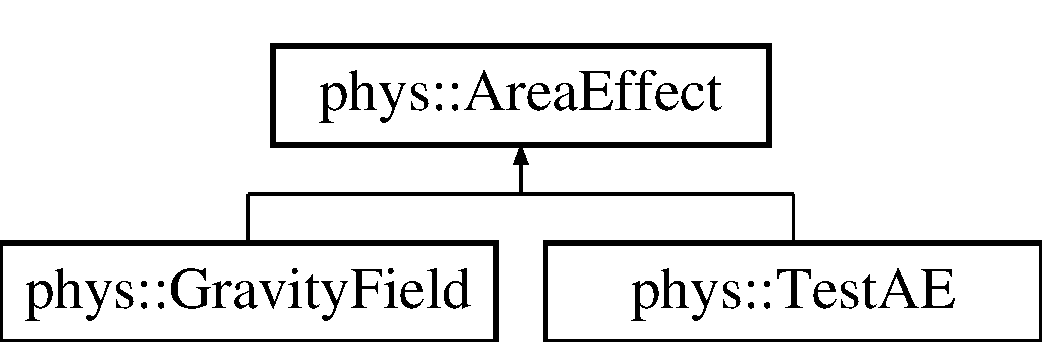
\includegraphics[height=2.000000cm]{d4/d55/classphys_1_1AreaEffect}
\end{center}
\end{figure}
\subsection*{Public Member Functions}
\begin{DoxyCompactItemize}
\item 
\hyperlink{classphys_1_1AreaEffect_a0c6710f348ab875cca41b613798f1f2a}{AreaEffect} (const \hyperlink{namespacephys_aa03900411993de7fbfec4789bc1d392e}{String} \&name, \hyperlink{classphys_1_1Vector3}{Vector3} Location)
\begin{DoxyCompactList}\small\item\em Constructor. \item\end{DoxyCompactList}\item 
virtual \hyperlink{classphys_1_1AreaEffect_aa9e6d721d337c32aa47357060d319924}{$\sim$AreaEffect} ()
\begin{DoxyCompactList}\small\item\em Destructor. \item\end{DoxyCompactList}\item 
virtual void \hyperlink{classphys_1_1AreaEffect_a3b285ecfcf9c9200662d510e48dd222a}{ApplyEffect} ()=0
\begin{DoxyCompactList}\small\item\em Defines and applies the effect of the field. \item\end{DoxyCompactList}\item 
virtual void \hyperlink{classphys_1_1AreaEffect_a0a0e6dfc6353d19b19e7bea037172072}{UpdateActorList} ()
\begin{DoxyCompactList}\small\item\em Updates the actors listed as within the field. \item\end{DoxyCompactList}\item 
void \hyperlink{classphys_1_1AreaEffect_aa794048d274ea12775b14de39171f14d}{CreateSphereShape} (\hyperlink{namespacephys_af7eb897198d265b8e868f45240230d5f}{Real} Radius)
\begin{DoxyCompactList}\small\item\em Creates a Sphere shape for the field. \item\end{DoxyCompactList}\item 
void \hyperlink{classphys_1_1AreaEffect_a7329a52fdd8382d19d39bed1ab2eea61}{CreateCylinderShape} (\hyperlink{classphys_1_1Vector3}{Vector3} HalfExtents)
\begin{DoxyCompactList}\small\item\em Creates a Cylinder shape for the field. \item\end{DoxyCompactList}\item 
void \hyperlink{classphys_1_1AreaEffect_ada171b33d232988b4a728f816217254d}{CreateBoxShape} (\hyperlink{classphys_1_1Vector3}{Vector3} HalfExtents)
\begin{DoxyCompactList}\small\item\em Creates a Box shape for the field. \item\end{DoxyCompactList}\item 
void \hyperlink{classphys_1_1AreaEffect_a341fb24b93bdd0994ce44ce0be571685}{CreateShapeFromMesh} (\hyperlink{namespacephys_aa03900411993de7fbfec4789bc1d392e}{String} Filename, \hyperlink{namespacephys_aa03900411993de7fbfec4789bc1d392e}{String} Group)
\begin{DoxyCompactList}\small\item\em Creates a shape from a .mesh model for the field. \item\end{DoxyCompactList}\item 
void \hyperlink{classphys_1_1AreaEffect_a0f906c38396ded16978423ad9acc4673}{ScaleFieldShape} (\hyperlink{classphys_1_1Vector3}{Vector3} Scale)
\begin{DoxyCompactList}\small\item\em Sets the scale of the shape of the field. \item\end{DoxyCompactList}\item 
\hyperlink{classphys_1_1Vector3}{Vector3} \hyperlink{classphys_1_1AreaEffect_a251d82e373c6ada5b80c023434e513f6}{GetFieldShapeScale} ()
\begin{DoxyCompactList}\small\item\em Gets the scale of the shape of the field. \item\end{DoxyCompactList}\item 
void \hyperlink{classphys_1_1AreaEffect_aeae24cc1087ad174d406a7a5117d0aed}{SetLocation} (\hyperlink{classphys_1_1Vector3}{Vector3} Location)
\begin{DoxyCompactList}\small\item\em Sets the origin for the area effect. \item\end{DoxyCompactList}\item 
\hyperlink{classphys_1_1Vector3}{Vector3} \hyperlink{classphys_1_1AreaEffect_a76040dd90ff314ea6973dccf4e90ba37}{GetLocation} ()
\begin{DoxyCompactList}\small\item\em Gets the origin for the area effect. \item\end{DoxyCompactList}\item 
\hyperlink{namespacephys_a5ce5049f8b4bf88d6413c47b504ebb31}{ConstString} \& \hyperlink{classphys_1_1AreaEffect_a6395eeec0a3aec2385027cca35cf15cb}{GetName} ()
\begin{DoxyCompactList}\small\item\em Gets the Area Effects name. \item\end{DoxyCompactList}\item 
std::list$<$ \hyperlink{classphys_1_1ActorBase}{ActorBase} $\ast$ $>$ \& \hyperlink{classphys_1_1AreaEffect_ab995fec11d9e5fbae1851109067958db}{GetOverlappingActors} ()
\begin{DoxyCompactList}\small\item\em Gets the list of actors within this field. \item\end{DoxyCompactList}\item 
std::vector$<$ \hyperlink{classphys_1_1ActorBase}{ActorBase} $\ast$ $>$ \& \hyperlink{classphys_1_1AreaEffect_a72a9673c926ce876df630c4aecfc09f6}{GetAddedActors} ()
\begin{DoxyCompactList}\small\item\em Gets the list of actors that have been added to the list since the last simulation step. \item\end{DoxyCompactList}\item 
std::vector$<$ \hyperlink{classphys_1_1ActorBase}{ActorBase} $\ast$ $>$ \& \hyperlink{classphys_1_1AreaEffect_a021763db69e977a3a19ad7cc39df073b}{GetRemovedActors} ()
\begin{DoxyCompactList}\small\item\em Gets the list of actors that have been removed from the list since the last simulation step. \item\end{DoxyCompactList}\end{DoxyCompactItemize}
\subsection*{Protected Member Functions}
\begin{DoxyCompactItemize}
\item 
virtual void \hyperlink{classphys_1_1AreaEffect_a31e4c0fee03dca66ba4c49727b20f58d}{CreateGhostObject} (\hyperlink{classphys_1_1Vector3}{Vector3} Location)
\begin{DoxyCompactList}\small\item\em Constructor Function. \item\end{DoxyCompactList}\item 
\hypertarget{classphys_1_1AreaEffect_a7af039b84f8d55e2c1c2d5a1b57afd8a}{
virtual void \hyperlink{classphys_1_1AreaEffect_a7af039b84f8d55e2c1c2d5a1b57afd8a}{AddActorToList} (\hyperlink{classphys_1_1ActorBase}{ActorBase} $\ast$Actor)}
\label{d4/d55/classphys_1_1AreaEffect_a7af039b84f8d55e2c1c2d5a1b57afd8a}

\begin{DoxyCompactList}\small\item\em Helper function for adding actors to relevant lists. \item\end{DoxyCompactList}\item 
\hypertarget{classphys_1_1AreaEffect_a98bf156da3c7f8bb98d5ce9d37b6aa0f}{
virtual void \hyperlink{classphys_1_1AreaEffect_a98bf156da3c7f8bb98d5ce9d37b6aa0f}{RemoveActorFromList} (\hyperlink{classphys_1_1ActorBase}{ActorBase} $\ast$Actor)}
\label{d4/d55/classphys_1_1AreaEffect_a98bf156da3c7f8bb98d5ce9d37b6aa0f}

\begin{DoxyCompactList}\small\item\em Helper function for adding actors to relevant lists. \item\end{DoxyCompactList}\end{DoxyCompactItemize}
\subsection*{Protected Attributes}
\begin{DoxyCompactItemize}
\item 
\hypertarget{classphys_1_1AreaEffect_a1cf5a878eb22b30a166f5b065944a986}{
\hyperlink{namespacephys_aa03900411993de7fbfec4789bc1d392e}{String} \hyperlink{classphys_1_1AreaEffect_a1cf5a878eb22b30a166f5b065944a986}{Name}}
\label{d4/d55/classphys_1_1AreaEffect_a1cf5a878eb22b30a166f5b065944a986}

\begin{DoxyCompactList}\small\item\em The name of the Area Effect. \item\end{DoxyCompactList}\item 
\hypertarget{classphys_1_1AreaEffect_af8189f9e8dc4bf04f44550918e0ee117}{
btCollisionShape $\ast$ \hyperlink{classphys_1_1AreaEffect_af8189f9e8dc4bf04f44550918e0ee117}{Shape}}
\label{d4/d55/classphys_1_1AreaEffect_af8189f9e8dc4bf04f44550918e0ee117}

\begin{DoxyCompactList}\small\item\em Stores the shape of the AE field. \item\end{DoxyCompactList}\item 
\hypertarget{classphys_1_1AreaEffect_ae730c591bf929404f337d71d4119bde8}{
btPairCachingGhostObject $\ast$ \hyperlink{classphys_1_1AreaEffect_ae730c591bf929404f337d71d4119bde8}{Ghost}}
\label{d4/d55/classphys_1_1AreaEffect_ae730c591bf929404f337d71d4119bde8}

\begin{DoxyCompactList}\small\item\em The object representing the AE field itself. \item\end{DoxyCompactList}\item 
\hypertarget{classphys_1_1AreaEffect_a3008e8e90236141ca4c21a9580e6f5de}{
\hyperlink{classphys_1_1World}{World} $\ast$ \hyperlink{classphys_1_1AreaEffect_a3008e8e90236141ca4c21a9580e6f5de}{TheWorld}}
\label{d4/d55/classphys_1_1AreaEffect_a3008e8e90236141ca4c21a9580e6f5de}

\begin{DoxyCompactList}\small\item\em \hyperlink{classphys_1_1World}{World} pointer simply to enable the effects of this class to be as diverse as the engine features. \item\end{DoxyCompactList}\item 
\hypertarget{classphys_1_1AreaEffect_a45834591f0ea49ba6657ce58d070ee9b}{
std::list$<$ \hyperlink{classphys_1_1ActorBase}{ActorBase} $\ast$ $>$ \hyperlink{classphys_1_1AreaEffect_a45834591f0ea49ba6657ce58d070ee9b}{OverlappingActors}}
\label{d4/d55/classphys_1_1AreaEffect_a45834591f0ea49ba6657ce58d070ee9b}

\begin{DoxyCompactList}\small\item\em Container for actors within the field area. \item\end{DoxyCompactList}\item 
\hypertarget{classphys_1_1AreaEffect_a5bd2ad15db98ecc140a8bf2fee8d0c1f}{
std::vector$<$ \hyperlink{classphys_1_1ActorBase}{ActorBase} $\ast$ $>$ \hyperlink{classphys_1_1AreaEffect_a5bd2ad15db98ecc140a8bf2fee8d0c1f}{AddedActors}}
\label{d4/d55/classphys_1_1AreaEffect_a5bd2ad15db98ecc140a8bf2fee8d0c1f}

\begin{DoxyCompactList}\small\item\em Container of actors that have been added since last frame. \item\end{DoxyCompactList}\item 
\hypertarget{classphys_1_1AreaEffect_a1b1b6cced61ead4d6de3d8bad5c2125a}{
std::vector$<$ \hyperlink{classphys_1_1ActorBase}{ActorBase} $\ast$ $>$ \hyperlink{classphys_1_1AreaEffect_a1b1b6cced61ead4d6de3d8bad5c2125a}{RemovedActors}}
\label{d4/d55/classphys_1_1AreaEffect_a1b1b6cced61ead4d6de3d8bad5c2125a}

\begin{DoxyCompactList}\small\item\em Container of actors that have been removed since last frame. \item\end{DoxyCompactList}\end{DoxyCompactItemize}
\subsection*{Friends}
\begin{DoxyCompactItemize}
\item 
\hypertarget{classphys_1_1AreaEffect_a139cf05ac01161b7071c8a037c841683}{
class {\bfseries PhysicsManager}}
\label{d4/d55/classphys_1_1AreaEffect_a139cf05ac01161b7071c8a037c841683}

\end{DoxyCompactItemize}


\subsection{Detailed Description}
This class is used to define area's in the world that have unique effects. Common uses for this class are for gravity fields, and explosions. But can be made to do more. \par
 Note: This is a base class intended to be derived from. This class cannot be created itself. To make an \hyperlink{classphys_1_1AreaEffect}{AreaEffect} class that does what you want it to, simple inherit from this class with an AE class of your own, and define the \hyperlink{classphys_1_1AreaEffect_a3b285ecfcf9c9200662d510e48dd222a}{ApplyEffect()} function to do what you want your effect to do. 

Definition at line 65 of file areaeffect.h.



\subsection{Constructor \& Destructor Documentation}
\hypertarget{classphys_1_1AreaEffect_a0c6710f348ab875cca41b613798f1f2a}{
\index{phys::AreaEffect@{phys::AreaEffect}!AreaEffect@{AreaEffect}}
\index{AreaEffect@{AreaEffect}!phys::AreaEffect@{phys::AreaEffect}}
\subsubsection[{AreaEffect}]{\setlength{\rightskip}{0pt plus 5cm}phys::AreaEffect::AreaEffect (
\begin{DoxyParamCaption}
\item[{const {\bf String} \&}]{ name, }
\item[{{\bf Vector3}}]{ Location}
\end{DoxyParamCaption}
)}}
\label{d4/d55/classphys_1_1AreaEffect_a0c6710f348ab875cca41b613798f1f2a}


Constructor. 

Basic initialization constructor. 
\begin{DoxyParams}{Parameters}
\item[{\em name}]The name of the field. \item[{\em Location}]The location of the AE field. \end{DoxyParams}


Definition at line 46 of file areaeffect.cpp.

\hypertarget{classphys_1_1AreaEffect_aa9e6d721d337c32aa47357060d319924}{
\index{phys::AreaEffect@{phys::AreaEffect}!$\sim$AreaEffect@{$\sim$AreaEffect}}
\index{$\sim$AreaEffect@{$\sim$AreaEffect}!phys::AreaEffect@{phys::AreaEffect}}
\subsubsection[{$\sim$AreaEffect}]{\setlength{\rightskip}{0pt plus 5cm}phys::AreaEffect::$\sim$AreaEffect (
\begin{DoxyParamCaption}
{}
\end{DoxyParamCaption}
)\hspace{0.3cm}{\ttfamily  \mbox{[}virtual\mbox{]}}}}
\label{d4/d55/classphys_1_1AreaEffect_aa9e6d721d337c32aa47357060d319924}


Destructor. 

Class destructor. 

Definition at line 53 of file areaeffect.cpp.



\subsection{Member Function Documentation}
\hypertarget{classphys_1_1AreaEffect_a3b285ecfcf9c9200662d510e48dd222a}{
\index{phys::AreaEffect@{phys::AreaEffect}!ApplyEffect@{ApplyEffect}}
\index{ApplyEffect@{ApplyEffect}!phys::AreaEffect@{phys::AreaEffect}}
\subsubsection[{ApplyEffect}]{\setlength{\rightskip}{0pt plus 5cm}virtual void phys::AreaEffect::ApplyEffect (
\begin{DoxyParamCaption}
{}
\end{DoxyParamCaption}
)\hspace{0.3cm}{\ttfamily  \mbox{[}pure virtual\mbox{]}}}}
\label{d4/d55/classphys_1_1AreaEffect_a3b285ecfcf9c9200662d510e48dd222a}


Defines and applies the effect of the field. 

When inheriting this class, this function is what defines the effect the field has. \par
 This function will be called on by the physics manager and shouldn't be called manually. 

Implemented in \hyperlink{classphys_1_1TestAE_a191c60dbfa277e850ea392d9ab774c42}{phys::TestAE}, and \hyperlink{classphys_1_1GravityField_a0322cb1635bbcb951493d9e17cc9acb1}{phys::GravityField}.

\hypertarget{classphys_1_1AreaEffect_ada171b33d232988b4a728f816217254d}{
\index{phys::AreaEffect@{phys::AreaEffect}!CreateBoxShape@{CreateBoxShape}}
\index{CreateBoxShape@{CreateBoxShape}!phys::AreaEffect@{phys::AreaEffect}}
\subsubsection[{CreateBoxShape}]{\setlength{\rightskip}{0pt plus 5cm}void phys::AreaEffect::CreateBoxShape (
\begin{DoxyParamCaption}
\item[{{\bf Vector3}}]{ HalfExtents}
\end{DoxyParamCaption}
)}}
\label{d4/d55/classphys_1_1AreaEffect_ada171b33d232988b4a728f816217254d}


Creates a Box shape for the field. 

When making the vector to be passed in, remember to pass in only half values of what you want the actual size to be. 
\begin{DoxyParams}{Parameters}
\item[{\em HalfExtents}]The vector representing the size of the shape. \end{DoxyParams}


Definition at line 158 of file areaeffect.cpp.

\hypertarget{classphys_1_1AreaEffect_a7329a52fdd8382d19d39bed1ab2eea61}{
\index{phys::AreaEffect@{phys::AreaEffect}!CreateCylinderShape@{CreateCylinderShape}}
\index{CreateCylinderShape@{CreateCylinderShape}!phys::AreaEffect@{phys::AreaEffect}}
\subsubsection[{CreateCylinderShape}]{\setlength{\rightskip}{0pt plus 5cm}void phys::AreaEffect::CreateCylinderShape (
\begin{DoxyParamCaption}
\item[{{\bf Vector3}}]{ HalfExtents}
\end{DoxyParamCaption}
)}}
\label{d4/d55/classphys_1_1AreaEffect_a7329a52fdd8382d19d39bed1ab2eea61}


Creates a Cylinder shape for the field. 

This function assumes the cylinder will be upright, meaning \char`\"{}up\char`\"{} will be on the positive Y axis. \par
 When making the vector to be passed in, remember the layout should be as such: (radius, height$\ast$0.5, radius). 
\begin{DoxyParams}{Parameters}
\item[{\em HalfExtents}]The vector representing the size of the shape. \end{DoxyParams}


Definition at line 152 of file areaeffect.cpp.

\hypertarget{classphys_1_1AreaEffect_a31e4c0fee03dca66ba4c49727b20f58d}{
\index{phys::AreaEffect@{phys::AreaEffect}!CreateGhostObject@{CreateGhostObject}}
\index{CreateGhostObject@{CreateGhostObject}!phys::AreaEffect@{phys::AreaEffect}}
\subsubsection[{CreateGhostObject}]{\setlength{\rightskip}{0pt plus 5cm}void phys::AreaEffect::CreateGhostObject (
\begin{DoxyParamCaption}
\item[{{\bf Vector3}}]{ Location}
\end{DoxyParamCaption}
)\hspace{0.3cm}{\ttfamily  \mbox{[}protected, virtual\mbox{]}}}}
\label{d4/d55/classphys_1_1AreaEffect_a31e4c0fee03dca66ba4c49727b20f58d}


Constructor Function. 


\begin{DoxyParams}{Parameters}
\item[{\em Location}]The location of the AE field. \end{DoxyParams}


Definition at line 59 of file areaeffect.cpp.

\hypertarget{classphys_1_1AreaEffect_a341fb24b93bdd0994ce44ce0be571685}{
\index{phys::AreaEffect@{phys::AreaEffect}!CreateShapeFromMesh@{CreateShapeFromMesh}}
\index{CreateShapeFromMesh@{CreateShapeFromMesh}!phys::AreaEffect@{phys::AreaEffect}}
\subsubsection[{CreateShapeFromMesh}]{\setlength{\rightskip}{0pt plus 5cm}void phys::AreaEffect::CreateShapeFromMesh (
\begin{DoxyParamCaption}
\item[{{\bf String}}]{ Filename, }
\item[{{\bf String}}]{ Group}
\end{DoxyParamCaption}
)}}
\label{d4/d55/classphys_1_1AreaEffect_a341fb24b93bdd0994ce44ce0be571685}


Creates a shape from a .mesh model for the field. 


\begin{DoxyParams}{Parameters}
\item[{\em Filename}]The name of the .mesh file to be used. \item[{\em Group}]The resource group where the mesh can be found. \end{DoxyParams}


Definition at line 164 of file areaeffect.cpp.

\hypertarget{classphys_1_1AreaEffect_aa794048d274ea12775b14de39171f14d}{
\index{phys::AreaEffect@{phys::AreaEffect}!CreateSphereShape@{CreateSphereShape}}
\index{CreateSphereShape@{CreateSphereShape}!phys::AreaEffect@{phys::AreaEffect}}
\subsubsection[{CreateSphereShape}]{\setlength{\rightskip}{0pt plus 5cm}void phys::AreaEffect::CreateSphereShape (
\begin{DoxyParamCaption}
\item[{{\bf Real}}]{ Radius}
\end{DoxyParamCaption}
)}}
\label{d4/d55/classphys_1_1AreaEffect_aa794048d274ea12775b14de39171f14d}


Creates a Sphere shape for the field. 


\begin{DoxyParams}{Parameters}
\item[{\em Radius}]The radius of the sphere you want to create. \end{DoxyParams}


Definition at line 146 of file areaeffect.cpp.

\hypertarget{classphys_1_1AreaEffect_a72a9673c926ce876df630c4aecfc09f6}{
\index{phys::AreaEffect@{phys::AreaEffect}!GetAddedActors@{GetAddedActors}}
\index{GetAddedActors@{GetAddedActors}!phys::AreaEffect@{phys::AreaEffect}}
\subsubsection[{GetAddedActors}]{\setlength{\rightskip}{0pt plus 5cm}std::vector$<$ {\bf ActorBase} $\ast$ $>$ \& phys::AreaEffect::GetAddedActors (
\begin{DoxyParamCaption}
{}
\end{DoxyParamCaption}
)}}
\label{d4/d55/classphys_1_1AreaEffect_a72a9673c926ce876df630c4aecfc09f6}


Gets the list of actors that have been added to the list since the last simulation step. 

\begin{DoxyReturn}{Returns}
Returns the vector storing all the actors that have been added to the list since the last simulation step. 
\end{DoxyReturn}


Definition at line 262 of file areaeffect.cpp.

\hypertarget{classphys_1_1AreaEffect_a251d82e373c6ada5b80c023434e513f6}{
\index{phys::AreaEffect@{phys::AreaEffect}!GetFieldShapeScale@{GetFieldShapeScale}}
\index{GetFieldShapeScale@{GetFieldShapeScale}!phys::AreaEffect@{phys::AreaEffect}}
\subsubsection[{GetFieldShapeScale}]{\setlength{\rightskip}{0pt plus 5cm}{\bf Vector3} phys::AreaEffect::GetFieldShapeScale (
\begin{DoxyParamCaption}
{}
\end{DoxyParamCaption}
)}}
\label{d4/d55/classphys_1_1AreaEffect_a251d82e373c6ada5b80c023434e513f6}


Gets the scale of the shape of the field. 

The default scale is 1.0. \begin{DoxyReturn}{Returns}
Returns the current scale applied to the fields shape. 
\end{DoxyReturn}


Definition at line 235 of file areaeffect.cpp.

\hypertarget{classphys_1_1AreaEffect_a76040dd90ff314ea6973dccf4e90ba37}{
\index{phys::AreaEffect@{phys::AreaEffect}!GetLocation@{GetLocation}}
\index{GetLocation@{GetLocation}!phys::AreaEffect@{phys::AreaEffect}}
\subsubsection[{GetLocation}]{\setlength{\rightskip}{0pt plus 5cm}{\bf Vector3} phys::AreaEffect::GetLocation (
\begin{DoxyParamCaption}
{}
\end{DoxyParamCaption}
)}}
\label{d4/d55/classphys_1_1AreaEffect_a76040dd90ff314ea6973dccf4e90ba37}


Gets the origin for the area effect. 

This function is particularly useful when making fields such as gravity wells, that have continuous effects centering on one location. \begin{DoxyReturn}{Returns}
Returns the vector3 representing the location of the area effect. 
\end{DoxyReturn}


Definition at line 246 of file areaeffect.cpp.

\hypertarget{classphys_1_1AreaEffect_a6395eeec0a3aec2385027cca35cf15cb}{
\index{phys::AreaEffect@{phys::AreaEffect}!GetName@{GetName}}
\index{GetName@{GetName}!phys::AreaEffect@{phys::AreaEffect}}
\subsubsection[{GetName}]{\setlength{\rightskip}{0pt plus 5cm}{\bf ConstString} \& phys::AreaEffect::GetName (
\begin{DoxyParamCaption}
{}
\end{DoxyParamCaption}
)}}
\label{d4/d55/classphys_1_1AreaEffect_a6395eeec0a3aec2385027cca35cf15cb}


Gets the Area Effects name. 

\begin{DoxyReturn}{Returns}
Returns the name of the Area Effect. 
\end{DoxyReturn}


Definition at line 252 of file areaeffect.cpp.

\hypertarget{classphys_1_1AreaEffect_ab995fec11d9e5fbae1851109067958db}{
\index{phys::AreaEffect@{phys::AreaEffect}!GetOverlappingActors@{GetOverlappingActors}}
\index{GetOverlappingActors@{GetOverlappingActors}!phys::AreaEffect@{phys::AreaEffect}}
\subsubsection[{GetOverlappingActors}]{\setlength{\rightskip}{0pt plus 5cm}std::list$<$ {\bf ActorBase} $\ast$ $>$ \& phys::AreaEffect::GetOverlappingActors (
\begin{DoxyParamCaption}
{}
\end{DoxyParamCaption}
)}}
\label{d4/d55/classphys_1_1AreaEffect_ab995fec11d9e5fbae1851109067958db}


Gets the list of actors within this field. 

\begin{DoxyReturn}{Returns}
Returns the list of actors contained within this field. 
\end{DoxyReturn}


Definition at line 257 of file areaeffect.cpp.

\hypertarget{classphys_1_1AreaEffect_a021763db69e977a3a19ad7cc39df073b}{
\index{phys::AreaEffect@{phys::AreaEffect}!GetRemovedActors@{GetRemovedActors}}
\index{GetRemovedActors@{GetRemovedActors}!phys::AreaEffect@{phys::AreaEffect}}
\subsubsection[{GetRemovedActors}]{\setlength{\rightskip}{0pt plus 5cm}std::vector$<$ {\bf ActorBase} $\ast$ $>$ \& phys::AreaEffect::GetRemovedActors (
\begin{DoxyParamCaption}
{}
\end{DoxyParamCaption}
)}}
\label{d4/d55/classphys_1_1AreaEffect_a021763db69e977a3a19ad7cc39df073b}


Gets the list of actors that have been removed from the list since the last simulation step. 

\begin{DoxyReturn}{Returns}
Returns the vector storing all the actors that have been removed from the list since the last simulation step. 
\end{DoxyReturn}


Definition at line 267 of file areaeffect.cpp.

\hypertarget{classphys_1_1AreaEffect_a0f906c38396ded16978423ad9acc4673}{
\index{phys::AreaEffect@{phys::AreaEffect}!ScaleFieldShape@{ScaleFieldShape}}
\index{ScaleFieldShape@{ScaleFieldShape}!phys::AreaEffect@{phys::AreaEffect}}
\subsubsection[{ScaleFieldShape}]{\setlength{\rightskip}{0pt plus 5cm}void phys::AreaEffect::ScaleFieldShape (
\begin{DoxyParamCaption}
\item[{{\bf Vector3}}]{ Scale}
\end{DoxyParamCaption}
)}}
\label{d4/d55/classphys_1_1AreaEffect_a0f906c38396ded16978423ad9acc4673}


Sets the scale of the shape of the field. 

The default scale is 1.0. 
\begin{DoxyParams}{Parameters}
\item[{\em Scale}]The vector3 representing the scale you wish to apply to each axis of the field shape. \end{DoxyParams}


Definition at line 230 of file areaeffect.cpp.

\hypertarget{classphys_1_1AreaEffect_aeae24cc1087ad174d406a7a5117d0aed}{
\index{phys::AreaEffect@{phys::AreaEffect}!SetLocation@{SetLocation}}
\index{SetLocation@{SetLocation}!phys::AreaEffect@{phys::AreaEffect}}
\subsubsection[{SetLocation}]{\setlength{\rightskip}{0pt plus 5cm}void phys::AreaEffect::SetLocation (
\begin{DoxyParamCaption}
\item[{{\bf Vector3}}]{ Location}
\end{DoxyParamCaption}
)}}
\label{d4/d55/classphys_1_1AreaEffect_aeae24cc1087ad174d406a7a5117d0aed}


Sets the origin for the area effect. 

In most cases you won't want to call this, with the exception of when you want a field to follow/track an actor. 
\begin{DoxyParams}{Parameters}
\item[{\em Location}]The updated location of the origin for the field. \end{DoxyParams}


Definition at line 241 of file areaeffect.cpp.

\hypertarget{classphys_1_1AreaEffect_a0a0e6dfc6353d19b19e7bea037172072}{
\index{phys::AreaEffect@{phys::AreaEffect}!UpdateActorList@{UpdateActorList}}
\index{UpdateActorList@{UpdateActorList}!phys::AreaEffect@{phys::AreaEffect}}
\subsubsection[{UpdateActorList}]{\setlength{\rightskip}{0pt plus 5cm}void phys::AreaEffect::UpdateActorList (
\begin{DoxyParamCaption}
{}
\end{DoxyParamCaption}
)\hspace{0.3cm}{\ttfamily  \mbox{[}virtual\mbox{]}}}}
\label{d4/d55/classphys_1_1AreaEffect_a0a0e6dfc6353d19b19e7bea037172072}


Updates the actors listed as within the field. 

This function is automatically called once every simulation step. This shouldn't be called manually unless your usage of this class requires more then one update per step. 

Definition at line 85 of file areaeffect.cpp.



The documentation for this class was generated from the following files:\begin{DoxyCompactItemize}
\item 
areaeffect.h\item 
areaeffect.cpp\end{DoxyCompactItemize}

\hypertarget{classphys_1_1Attachable}{
\section{phys::Attachable Class Reference}
\label{df/dbd/classphys_1_1Attachable}\index{phys::Attachable@{phys::Attachable}}
}


This is just a base class to be used by elements that are attachable to nodes.  




{\ttfamily \#include $<$attachable.h$>$}

Inheritance diagram for phys::Attachable:\begin{figure}[H]
\begin{center}
\leavevmode
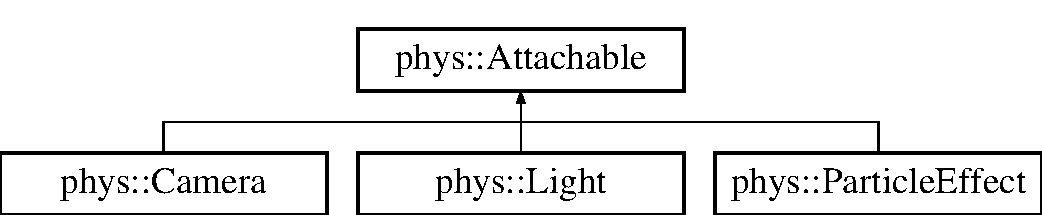
\includegraphics[height=2.000000cm]{df/dbd/classphys_1_1Attachable}
\end{center}
\end{figure}
\subsection*{Public Types}
\begin{DoxyCompactItemize}
\item 
enum {\bfseries AttachableElement} \{ {\bfseries Camera}, 
{\bfseries Light}, 
{\bfseries ParticleEffect}
 \}
\end{DoxyCompactItemize}
\subsection*{Public Member Functions}
\begin{DoxyCompactItemize}
\item 
\hypertarget{classphys_1_1Attachable_a93c18f22769a1f70ae300fc2c58210eb}{
\hyperlink{classphys_1_1Attachable_a93c18f22769a1f70ae300fc2c58210eb}{Attachable} ()}
\label{df/dbd/classphys_1_1Attachable_a93c18f22769a1f70ae300fc2c58210eb}

\begin{DoxyCompactList}\small\item\em No initialization class constructor. \item\end{DoxyCompactList}\item 
\hypertarget{classphys_1_1Attachable_af7187e29053b7fe339634394883729d4}{
virtual \hyperlink{classphys_1_1Attachable_af7187e29053b7fe339634394883729d4}{$\sim$Attachable} ()}
\label{df/dbd/classphys_1_1Attachable_af7187e29053b7fe339634394883729d4}

\begin{DoxyCompactList}\small\item\em Class destructor. \item\end{DoxyCompactList}\item 
Attachable::AttachableElement \hyperlink{classphys_1_1Attachable_a5f747000367afd85dfaff3a37976e74c}{GetElementType} ()
\begin{DoxyCompactList}\small\item\em Gets the type of element this is. \item\end{DoxyCompactList}\item 
\hypertarget{classphys_1_1Attachable_ad1a9bbd300fe21c5cc7e5aa7e2c95b85}{
virtual \hyperlink{namespacephys_aa03900411993de7fbfec4789bc1d392e}{String} \& \hyperlink{classphys_1_1Attachable_ad1a9bbd300fe21c5cc7e5aa7e2c95b85}{GetName} ()=0}
\label{df/dbd/classphys_1_1Attachable_ad1a9bbd300fe21c5cc7e5aa7e2c95b85}

\begin{DoxyCompactList}\small\item\em Gets the name of the attachable element. \item\end{DoxyCompactList}\end{DoxyCompactItemize}
\subsection*{Protected Member Functions}
\begin{DoxyCompactItemize}
\item 
void \hyperlink{classphys_1_1Attachable_a74361315eba9e4f0ce288518c92541fa}{SetElementType} (Attachable::AttachableElement Type)
\begin{DoxyCompactList}\small\item\em Sets the type of element this class is. \item\end{DoxyCompactList}\end{DoxyCompactItemize}
\subsection*{Protected Attributes}
\begin{DoxyCompactItemize}
\item 
\hypertarget{classphys_1_1Attachable_af574d5f08a304c6e0ae002bb2fc057c7}{
Attachable::AttachableElement \hyperlink{classphys_1_1Attachable_af574d5f08a304c6e0ae002bb2fc057c7}{ElementType}}
\label{df/dbd/classphys_1_1Attachable_af574d5f08a304c6e0ae002bb2fc057c7}

\begin{DoxyCompactList}\small\item\em Enum value representing the type of element this is. \item\end{DoxyCompactList}\end{DoxyCompactItemize}


\subsection{Detailed Description}
This is just a base class to be used by elements that are attachable to nodes. This class is useless on it's own and should not be created manually. 

Definition at line 54 of file attachable.h.



\subsection{Member Function Documentation}
\hypertarget{classphys_1_1Attachable_a5f747000367afd85dfaff3a37976e74c}{
\index{phys::Attachable@{phys::Attachable}!GetElementType@{GetElementType}}
\index{GetElementType@{GetElementType}!phys::Attachable@{phys::Attachable}}
\subsubsection[{GetElementType}]{\setlength{\rightskip}{0pt plus 5cm}Attachable::AttachableElement phys::Attachable::GetElementType (
\begin{DoxyParamCaption}
{}
\end{DoxyParamCaption}
)}}
\label{df/dbd/classphys_1_1Attachable_a5f747000367afd85dfaff3a37976e74c}


Gets the type of element this is. 

\begin{DoxyReturn}{Returns}
Returns an enum value indicating what type of element this is. 
\end{DoxyReturn}


Definition at line 60 of file attachable.cpp.

\hypertarget{classphys_1_1Attachable_a74361315eba9e4f0ce288518c92541fa}{
\index{phys::Attachable@{phys::Attachable}!SetElementType@{SetElementType}}
\index{SetElementType@{SetElementType}!phys::Attachable@{phys::Attachable}}
\subsubsection[{SetElementType}]{\setlength{\rightskip}{0pt plus 5cm}void phys::Attachable::SetElementType (
\begin{DoxyParamCaption}
\item[{Attachable::AttachableElement}]{ Type}
\end{DoxyParamCaption}
)\hspace{0.3cm}{\ttfamily  \mbox{[}protected\mbox{]}}}}
\label{df/dbd/classphys_1_1Attachable_a74361315eba9e4f0ce288518c92541fa}


Sets the type of element this class is. 


\begin{DoxyParams}{Parameters}
\item[{\em Enum}]value representing the type of element to be set. \end{DoxyParams}


Definition at line 55 of file attachable.cpp.



The documentation for this class was generated from the following files:\begin{DoxyCompactItemize}
\item 
attachable.h\item 
attachable.cpp\end{DoxyCompactItemize}

\hypertarget{classphys_1_1xml_1_1Attribute}{
\section{phys::xml::Attribute Class Reference}
\label{da/ddf/classphys_1_1xml_1_1Attribute}\index{phys::xml::Attribute@{phys::xml::Attribute}}
}


This represents the attributes that could exist on an XML element.  




{\ttfamily \#include $<$xmlattribute.h$>$}

Inheritance diagram for phys::xml::Attribute:\begin{figure}[H]
\begin{center}
\leavevmode
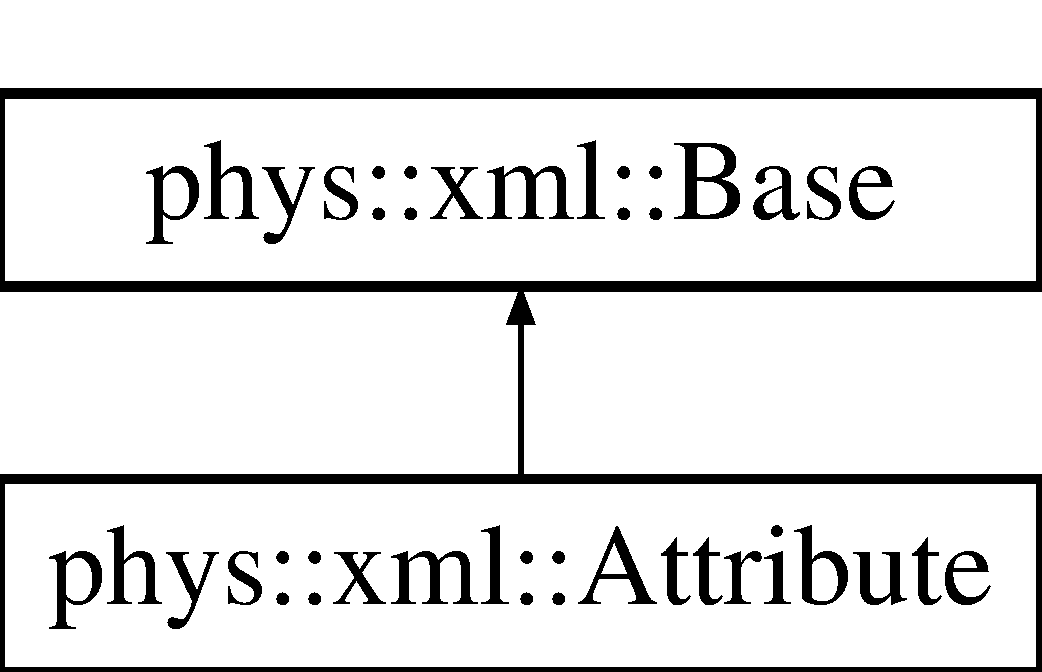
\includegraphics[height=2cm]{da/ddf/classphys_1_1xml_1_1Attribute}
\end{center}
\end{figure}
\subsection*{Public Member Functions}
\begin{DoxyCompactItemize}
\item 
\hypertarget{classphys_1_1xml_1_1Attribute_a962ad273e447bb714925c331e00cc3e7}{
\hyperlink{classphys_1_1xml_1_1Attribute_a962ad273e447bb714925c331e00cc3e7}{Attribute} ()}
\label{da/ddf/classphys_1_1xml_1_1Attribute_a962ad273e447bb714925c331e00cc3e7}

\begin{DoxyCompactList}\small\item\em Construct an empty attribute. \item\end{DoxyCompactList}\item 
\hypertarget{classphys_1_1xml_1_1Attribute_a2918dbce8208751944d3803a1300a914}{
\hyperlink{classphys_1_1xml_1_1Attribute_a2918dbce8208751944d3803a1300a914}{$\sim$Attribute} ()}
\label{da/ddf/classphys_1_1xml_1_1Attribute_a2918dbce8208751944d3803a1300a914}

\begin{DoxyCompactList}\small\item\em Tears down an attribute and removes the node from the DOM. \item\end{DoxyCompactList}\item 
\hyperlink{classphys_1_1xml_1_1Attribute_abce6652f3a2ca2cf5a5d46b7ceb1e108}{Attribute} (const \hyperlink{namespacephys_aa03900411993de7fbfec4789bc1d392e}{String} \&name, const \hyperlink{namespacephys_aa03900411993de7fbfec4789bc1d392e}{String} \&value)
\begin{DoxyCompactList}\small\item\em Construct an attribute with name and value. \item\end{DoxyCompactList}\item 
\hyperlink{namespacephys_aa03900411993de7fbfec4789bc1d392e}{String} \hyperlink{classphys_1_1xml_1_1Attribute_a9fda8a6a6a292639e2ef88c479c80d88}{GetValue} () const 
\begin{DoxyCompactList}\small\item\em Get the value of this attribute. \item\end{DoxyCompactList}\item 
void \hyperlink{classphys_1_1xml_1_1Attribute_a45b441e83fb3c6e0cc911019b61039ba}{SetValue} (const \hyperlink{namespacephys_a460f6bc24c8dd347b05e0366ae34f34a}{Whole} \&value)
\begin{DoxyCompactList}\small\item\em Set the value of this node. \item\end{DoxyCompactList}\item 
void \hyperlink{classphys_1_1xml_1_1Attribute_ad2ba3ccf96388f0c859bc90e45ed94ab}{SetValue} (const \hyperlink{namespacephys_af7eb897198d265b8e868f45240230d5f}{Real} \&value)
\begin{DoxyCompactList}\small\item\em Set the value of this node. \item\end{DoxyCompactList}\item 
void \hyperlink{classphys_1_1xml_1_1Attribute_ad06e8d677bfa76d43936bd97ac3e62ef}{SetValue} (const \hyperlink{namespacephys_aa03900411993de7fbfec4789bc1d392e}{String} \&value)
\begin{DoxyCompactList}\small\item\em Set the value of this node. \item\end{DoxyCompactList}\item 
void \hyperlink{classphys_1_1xml_1_1Attribute_a9c90f6c8b6c409309fd503e1fe4a71bd}{SetName} (const \hyperlink{namespacephys_aa03900411993de7fbfec4789bc1d392e}{String} \&Name)
\begin{DoxyCompactList}\small\item\em Set the Name of this attribute. \item\end{DoxyCompactList}\item 
\hyperlink{namespacephys_aa03900411993de7fbfec4789bc1d392e}{String} \hyperlink{classphys_1_1xml_1_1Attribute_a30314ef60f51e5e161ee4d9e2b6fbd6c}{GetName} () const 
\begin{DoxyCompactList}\small\item\em Get the Name of this attribute. \item\end{DoxyCompactList}\item 
\hyperlink{classphys_1_1xml_1_1Attribute}{Attribute} $\ast$ \hyperlink{classphys_1_1xml_1_1Attribute_aadf4930c5c1cd8aa140bea3c05253446}{Next} (bool throwIfNoAttribute=true) const 
\begin{DoxyCompactList}\small\item\em Get the next sibling attribute in the DOM. \item\end{DoxyCompactList}\item 
\hyperlink{classphys_1_1xml_1_1Attribute}{Attribute} $\ast$ \hyperlink{classphys_1_1xml_1_1Attribute_a3c9fdaa3f88cdf90d61af77cb33e022e}{Previous} (bool throwIfNoAttribute=true) const 
\begin{DoxyCompactList}\small\item\em Get the Previous sibling attribute in the DOM. \item\end{DoxyCompactList}\item 
virtual \hyperlink{classphys_1_1xml_1_1Base_a62ba0484b5ecb502f9ae9d82d3720320}{XMLComponentType} \hyperlink{classphys_1_1xml_1_1Attribute_a58ebb56547b77dad9c8cb11eb4558cc9}{GetType} ()
\begin{DoxyCompactList}\small\item\em This identifies what kind of child of xml::base this is. \item\end{DoxyCompactList}\end{DoxyCompactItemize}
\subsection*{Protected Member Functions}
\begin{DoxyCompactItemize}
\item 
\hypertarget{classphys_1_1xml_1_1Attribute_aeea008baed4c687e9ed9e1f3563f0c01}{
\hyperlink{classphys_1_1xml_1_1Attribute_aeea008baed4c687e9ed9e1f3563f0c01}{Attribute} (ticpp::Attribute $\ast$Meta)}
\label{da/ddf/classphys_1_1xml_1_1Attribute_aeea008baed4c687e9ed9e1f3563f0c01}

\begin{DoxyCompactList}\small\item\em Construct an attribute using meta data from a TiCPP pointer. \item\end{DoxyCompactList}\end{DoxyCompactItemize}


\subsection{Detailed Description}
This represents the attributes that could exist on an XML element. 

Definition at line 59 of file xmlattribute.h.



\subsection{Constructor \& Destructor Documentation}
\hypertarget{classphys_1_1xml_1_1Attribute_abce6652f3a2ca2cf5a5d46b7ceb1e108}{
\index{phys::xml::Attribute@{phys::xml::Attribute}!Attribute@{Attribute}}
\index{Attribute@{Attribute}!phys::xml::Attribute@{phys::xml::Attribute}}
\subsubsection[{Attribute}]{\setlength{\rightskip}{0pt plus 5cm}phys::xml::Attribute::Attribute (const {\bf String} \& {\em name}, \/  const {\bf String} \& {\em value})}}
\label{da/ddf/classphys_1_1xml_1_1Attribute_abce6652f3a2ca2cf5a5d46b7ceb1e108}


Construct an attribute with name and value. 


\begin{DoxyParams}{Parameters}
\item[{\em name}]What the \hyperlink{classphys_1_1xml_1_1Attribute}{Attribute} is called for example in \char`\"{} $<$div style=\char`\"{}14\char`\"{}$>$Content$<$/div$>$ \char`\"{} the word \char`\"{}style\char`\"{} is the attribute name \item[{\em value}]What the \hyperlink{classphys_1_1xml_1_1Attribute}{Attribute} is called for example in \char`\"{} $<$div style=\char`\"{}14\char`\"{}$>$Content$<$/div$>$ \char`\"{} the word \char`\"{}14\char`\"{} is the attribute value \end{DoxyParams}


Definition at line 56 of file xmlattribute.cpp.



\subsection{Member Function Documentation}
\hypertarget{classphys_1_1xml_1_1Attribute_a30314ef60f51e5e161ee4d9e2b6fbd6c}{
\index{phys::xml::Attribute@{phys::xml::Attribute}!GetName@{GetName}}
\index{GetName@{GetName}!phys::xml::Attribute@{phys::xml::Attribute}}
\subsubsection[{GetName}]{\setlength{\rightskip}{0pt plus 5cm}{\bf String} phys::xml::Attribute::GetName () const}}
\label{da/ddf/classphys_1_1xml_1_1Attribute_a30314ef60f51e5e161ee4d9e2b6fbd6c}


Get the Name of this attribute. 

\begin{DoxyReturn}{Returns}
This returns a String containing the name 
\end{DoxyReturn}


Definition at line 80 of file xmlattribute.cpp.

\hypertarget{classphys_1_1xml_1_1Attribute_a58ebb56547b77dad9c8cb11eb4558cc9}{
\index{phys::xml::Attribute@{phys::xml::Attribute}!GetType@{GetType}}
\index{GetType@{GetType}!phys::xml::Attribute@{phys::xml::Attribute}}
\subsubsection[{GetType}]{\setlength{\rightskip}{0pt plus 5cm}{\bf Attribute::XMLComponentType} phys::xml::Attribute::GetType ()\hspace{0.3cm}{\ttfamily  \mbox{[}virtual\mbox{]}}}}
\label{da/ddf/classphys_1_1xml_1_1Attribute_a58ebb56547b77dad9c8cb11eb4558cc9}


This identifies what kind of child of xml::base this is. 

\begin{DoxyReturn}{Returns}
This returns \hyperlink{classphys_1_1xml_1_1Base_a62ba0484b5ecb502f9ae9d82d3720320af75393e041247190be1c922d0b3faf07}{Base::isAttribute} 
\end{DoxyReturn}


Implements \hyperlink{classphys_1_1xml_1_1Base_af2821c239b5eb31c2524a499bf3ff19f}{phys::xml::Base}.



Definition at line 89 of file xmlattribute.cpp.

\hypertarget{classphys_1_1xml_1_1Attribute_a9fda8a6a6a292639e2ef88c479c80d88}{
\index{phys::xml::Attribute@{phys::xml::Attribute}!GetValue@{GetValue}}
\index{GetValue@{GetValue}!phys::xml::Attribute@{phys::xml::Attribute}}
\subsubsection[{GetValue}]{\setlength{\rightskip}{0pt plus 5cm}{\bf String} phys::xml::Attribute::GetValue () const}}
\label{da/ddf/classphys_1_1xml_1_1Attribute_a9fda8a6a6a292639e2ef88c479c80d88}


Get the value of this attribute. 

\begin{DoxyReturn}{Returns}
this returns a String containing the value of this attribute. 
\end{DoxyReturn}


Definition at line 65 of file xmlattribute.cpp.

\hypertarget{classphys_1_1xml_1_1Attribute_aadf4930c5c1cd8aa140bea3c05253446}{
\index{phys::xml::Attribute@{phys::xml::Attribute}!Next@{Next}}
\index{Next@{Next}!phys::xml::Attribute@{phys::xml::Attribute}}
\subsubsection[{Next}]{\setlength{\rightskip}{0pt plus 5cm}{\bf Attribute} $\ast$ phys::xml::Attribute::Next (bool {\em throwIfNoAttribute} = {\ttfamily true}) const}}
\label{da/ddf/classphys_1_1xml_1_1Attribute_aadf4930c5c1cd8aa140bea3c05253446}


Get the next sibling attribute in the DOM. 

\begin{DoxyWarning}{Warning}
This will cause memory leaks if the created pointer is not deleted 
\end{DoxyWarning}

\begin{DoxyParams}{Parameters}
\item[{\em throwIfNo}]\hyperlink{classphys_1_1xml_1_1Attribute}{Attribute} Should this function throw an exception if it fails, or silently fail. Defaults to true so it throws errors on failure. \end{DoxyParams}
\begin{DoxyReturn}{Returns}
Returns a pointer to an XML::Attribute that comes after this one, but still on the same element 
\end{DoxyReturn}


Definition at line 83 of file xmlattribute.cpp.

\hypertarget{classphys_1_1xml_1_1Attribute_a3c9fdaa3f88cdf90d61af77cb33e022e}{
\index{phys::xml::Attribute@{phys::xml::Attribute}!Previous@{Previous}}
\index{Previous@{Previous}!phys::xml::Attribute@{phys::xml::Attribute}}
\subsubsection[{Previous}]{\setlength{\rightskip}{0pt plus 5cm}{\bf Attribute} $\ast$ phys::xml::Attribute::Previous (bool {\em throwIfNoAttribute} = {\ttfamily true}) const}}
\label{da/ddf/classphys_1_1xml_1_1Attribute_a3c9fdaa3f88cdf90d61af77cb33e022e}


Get the Previous sibling attribute in the DOM. 

\begin{DoxyWarning}{Warning}
This will cause memory leaks if the created pointer is not deleted 
\end{DoxyWarning}

\begin{DoxyParams}{Parameters}
\item[{\em throwIfNo}]\hyperlink{classphys_1_1xml_1_1Attribute}{Attribute} Should this function throw an exception if it fails, or silently fail. Defaults to true so it throws errors on failure. \end{DoxyParams}
\begin{DoxyReturn}{Returns}
Returns a pointer to an XML::Attribute that comes before this one, but still on the same element. 
\end{DoxyReturn}


Definition at line 86 of file xmlattribute.cpp.

\hypertarget{classphys_1_1xml_1_1Attribute_a9c90f6c8b6c409309fd503e1fe4a71bd}{
\index{phys::xml::Attribute@{phys::xml::Attribute}!SetName@{SetName}}
\index{SetName@{SetName}!phys::xml::Attribute@{phys::xml::Attribute}}
\subsubsection[{SetName}]{\setlength{\rightskip}{0pt plus 5cm}void phys::xml::Attribute::SetName (const {\bf String} \& {\em Name})}}
\label{da/ddf/classphys_1_1xml_1_1Attribute_a9c90f6c8b6c409309fd503e1fe4a71bd}


Set the Name of this attribute. 


\begin{DoxyParams}{Parameters}
\item[{\em name}]A String that is the name the attribute will have. \end{DoxyParams}


Definition at line 77 of file xmlattribute.cpp.

\hypertarget{classphys_1_1xml_1_1Attribute_ad06e8d677bfa76d43936bd97ac3e62ef}{
\index{phys::xml::Attribute@{phys::xml::Attribute}!SetValue@{SetValue}}
\index{SetValue@{SetValue}!phys::xml::Attribute@{phys::xml::Attribute}}
\subsubsection[{SetValue}]{\setlength{\rightskip}{0pt plus 5cm}void phys::xml::Attribute::SetValue (const {\bf String} \& {\em value})}}
\label{da/ddf/classphys_1_1xml_1_1Attribute_ad06e8d677bfa76d43936bd97ac3e62ef}


Set the value of this node. 


\begin{DoxyParams}{Parameters}
\item[{\em value}]A String number to be inserted into the XML document \end{DoxyParams}


Definition at line 74 of file xmlattribute.cpp.

\hypertarget{classphys_1_1xml_1_1Attribute_ad2ba3ccf96388f0c859bc90e45ed94ab}{
\index{phys::xml::Attribute@{phys::xml::Attribute}!SetValue@{SetValue}}
\index{SetValue@{SetValue}!phys::xml::Attribute@{phys::xml::Attribute}}
\subsubsection[{SetValue}]{\setlength{\rightskip}{0pt plus 5cm}void phys::xml::Attribute::SetValue (const {\bf Real} \& {\em value})}}
\label{da/ddf/classphys_1_1xml_1_1Attribute_ad2ba3ccf96388f0c859bc90e45ed94ab}


Set the value of this node. 


\begin{DoxyParams}{Parameters}
\item[{\em value}]A Real number to be inserted into the XML document \end{DoxyParams}


Definition at line 71 of file xmlattribute.cpp.

\hypertarget{classphys_1_1xml_1_1Attribute_a45b441e83fb3c6e0cc911019b61039ba}{
\index{phys::xml::Attribute@{phys::xml::Attribute}!SetValue@{SetValue}}
\index{SetValue@{SetValue}!phys::xml::Attribute@{phys::xml::Attribute}}
\subsubsection[{SetValue}]{\setlength{\rightskip}{0pt plus 5cm}void phys::xml::Attribute::SetValue (const {\bf Whole} \& {\em value})}}
\label{da/ddf/classphys_1_1xml_1_1Attribute_a45b441e83fb3c6e0cc911019b61039ba}


Set the value of this node. 


\begin{DoxyParams}{Parameters}
\item[{\em value}]A Whole number to be inserted into the XML document \end{DoxyParams}


Definition at line 68 of file xmlattribute.cpp.



The documentation for this class was generated from the following files:\begin{DoxyCompactItemize}
\item 
\hyperlink{xmlattribute_8h}{xmlattribute.h}\item 
xmlattribute.cpp\end{DoxyCompactItemize}

\hypertarget{classphys_1_1xml_1_1AttributeIterator}{
\section{phys::xml::AttributeIterator Class Reference}
\label{de/d78/classphys_1_1xml_1_1AttributeIterator}\index{phys::xml::AttributeIterator@{phys::xml::AttributeIterator}}
}
\subsection*{Public Types}
\begin{DoxyCompactItemize}
\item 
\hypertarget{classphys_1_1xml_1_1AttributeIterator_a04d891c0ff2a2122b8122dd872e4237e}{
typedef ptrdiff\_\-t {\bfseries difference\_\-type}}
\label{de/d78/classphys_1_1xml_1_1AttributeIterator_a04d891c0ff2a2122b8122dd872e4237e}

\item 
\hypertarget{classphys_1_1xml_1_1AttributeIterator_a686c1153e4f2c76a47b9160751cf4ebf}{
typedef \hyperlink{classphys_1_1xml_1_1Attribute}{Attribute} {\bfseries value\_\-type}}
\label{de/d78/classphys_1_1xml_1_1AttributeIterator_a686c1153e4f2c76a47b9160751cf4ebf}

\item 
\hypertarget{classphys_1_1xml_1_1AttributeIterator_ab145be8859ba19f330b0e784343499e8}{
typedef \hyperlink{classphys_1_1xml_1_1Attribute}{Attribute} $\ast$ {\bfseries pointer}}
\label{de/d78/classphys_1_1xml_1_1AttributeIterator_ab145be8859ba19f330b0e784343499e8}

\item 
\hypertarget{classphys_1_1xml_1_1AttributeIterator_a9227aa824303a24a85124db7af006511}{
typedef \hyperlink{classphys_1_1xml_1_1Attribute}{Attribute} \& {\bfseries reference}}
\label{de/d78/classphys_1_1xml_1_1AttributeIterator_a9227aa824303a24a85124db7af006511}

\item 
\hypertarget{classphys_1_1xml_1_1AttributeIterator_aa34a1f322d8b952c25b52722db453d34}{
typedef std::bidirectional\_\-iterator\_\-tag {\bfseries iterator\_\-category}}
\label{de/d78/classphys_1_1xml_1_1AttributeIterator_aa34a1f322d8b952c25b52722db453d34}

\end{DoxyCompactItemize}
\subsection*{Public Member Functions}
\begin{DoxyCompactItemize}
\item 
\hypertarget{classphys_1_1xml_1_1AttributeIterator_ae338589383381586c8d8e5d893e498be}{
{\bfseries AttributeIterator} (const \hyperlink{classphys_1_1xml_1_1Attribute}{Attribute} \&attr, const \hyperlink{classphys_1_1xml_1_1Node}{Node} \&parent)}
\label{de/d78/classphys_1_1xml_1_1AttributeIterator_ae338589383381586c8d8e5d893e498be}

\item 
\hypertarget{classphys_1_1xml_1_1AttributeIterator_a5310ea26bd19cb1c32e962c03ea0dc62}{
bool {\bfseries operator==} (const \hyperlink{classphys_1_1xml_1_1AttributeIterator}{AttributeIterator} \&rhs) const }
\label{de/d78/classphys_1_1xml_1_1AttributeIterator_a5310ea26bd19cb1c32e962c03ea0dc62}

\item 
\hypertarget{classphys_1_1xml_1_1AttributeIterator_a6b80c4c5317f97921511e25597a3403f}{
bool {\bfseries operator!=} (const \hyperlink{classphys_1_1xml_1_1AttributeIterator}{AttributeIterator} \&rhs) const }
\label{de/d78/classphys_1_1xml_1_1AttributeIterator_a6b80c4c5317f97921511e25597a3403f}

\item 
\hypertarget{classphys_1_1xml_1_1AttributeIterator_a75fd50f268f3083378bff933999979c9}{
\hyperlink{classphys_1_1xml_1_1Attribute}{Attribute} \& {\bfseries operator$\ast$} ()}
\label{de/d78/classphys_1_1xml_1_1AttributeIterator_a75fd50f268f3083378bff933999979c9}

\item 
\hypertarget{classphys_1_1xml_1_1AttributeIterator_a4baca2564631c3683a5865955c4c8150}{
\hyperlink{classphys_1_1xml_1_1Attribute}{Attribute} $\ast$ {\bfseries operator-\/$>$} ()}
\label{de/d78/classphys_1_1xml_1_1AttributeIterator_a4baca2564631c3683a5865955c4c8150}

\item 
\hypertarget{classphys_1_1xml_1_1AttributeIterator_a32ffe54fee5136f533dcdf4877223c7e}{
const \hyperlink{classphys_1_1xml_1_1AttributeIterator}{AttributeIterator} \& {\bfseries operator++} ()}
\label{de/d78/classphys_1_1xml_1_1AttributeIterator_a32ffe54fee5136f533dcdf4877223c7e}

\item 
\hypertarget{classphys_1_1xml_1_1AttributeIterator_a9925e89424ac0d02453df60b4a8f21a7}{
\hyperlink{classphys_1_1xml_1_1AttributeIterator}{AttributeIterator} {\bfseries operator++} (int)}
\label{de/d78/classphys_1_1xml_1_1AttributeIterator_a9925e89424ac0d02453df60b4a8f21a7}

\item 
\hypertarget{classphys_1_1xml_1_1AttributeIterator_a0fab0cb1b2d3c779ab5c7215a11fc543}{
const \hyperlink{classphys_1_1xml_1_1AttributeIterator}{AttributeIterator} \& {\bfseries operator-\/-\/} ()}
\label{de/d78/classphys_1_1xml_1_1AttributeIterator_a0fab0cb1b2d3c779ab5c7215a11fc543}

\item 
\hypertarget{classphys_1_1xml_1_1AttributeIterator_ae46ebed7b404ae085c47984f615a7597}{
\hyperlink{classphys_1_1xml_1_1AttributeIterator}{AttributeIterator} {\bfseries operator-\/-\/} (int)}
\label{de/d78/classphys_1_1xml_1_1AttributeIterator_ae46ebed7b404ae085c47984f615a7597}

\end{DoxyCompactItemize}
\subsection*{Friends}
\begin{DoxyCompactItemize}
\item 
\hypertarget{classphys_1_1xml_1_1AttributeIterator_a6db9d28bd448a131448276ee03de1e6d}{
class {\bfseries Node}}
\label{de/d78/classphys_1_1xml_1_1AttributeIterator_a6db9d28bd448a131448276ee03de1e6d}

\end{DoxyCompactItemize}


\subsection{Detailed Description}


Definition at line 678 of file xml.h.



The documentation for this class was generated from the following file:\begin{DoxyCompactItemize}
\item 
\hyperlink{xml_8h}{xml.h}\end{DoxyCompactItemize}

\hypertarget{structphys_1_1xml_1_1AttributeStruct}{
\section{phys::xml::AttributeStruct Struct Reference}
\label{dd/dfe/structphys_1_1xml_1_1AttributeStruct}\index{phys::xml::AttributeStruct@{phys::xml::AttributeStruct}}
}
\subsection*{Public Member Functions}
\begin{DoxyCompactItemize}
\item 
\hypertarget{structphys_1_1xml_1_1AttributeStruct_ae56b37b04de2de9b06f2ab62063860d0}{
{\bfseries AttributeStruct} (MemoryPage $\ast$page)}
\label{dd/dfe/structphys_1_1xml_1_1AttributeStruct_ae56b37b04de2de9b06f2ab62063860d0}

\end{DoxyCompactItemize}
\subsection*{Public Attributes}
\begin{DoxyCompactItemize}
\item 
\hypertarget{structphys_1_1xml_1_1AttributeStruct_a9fd6577532fd75614cbbeef25ebc483d}{
uintptr\_\-t {\bfseries header}}
\label{dd/dfe/structphys_1_1xml_1_1AttributeStruct_a9fd6577532fd75614cbbeef25ebc483d}

\item 
\hypertarget{structphys_1_1xml_1_1AttributeStruct_af33547ea3e8c21d16737fc7ebcb94c95}{
char\_\-t $\ast$ {\bfseries Name}}
\label{dd/dfe/structphys_1_1xml_1_1AttributeStruct_af33547ea3e8c21d16737fc7ebcb94c95}

\item 
\hypertarget{structphys_1_1xml_1_1AttributeStruct_a2a7018296eb97ef342b5230d59f6e6ee}{
char\_\-t $\ast$ {\bfseries Value}}
\label{dd/dfe/structphys_1_1xml_1_1AttributeStruct_a2a7018296eb97ef342b5230d59f6e6ee}

\item 
\hypertarget{structphys_1_1xml_1_1AttributeStruct_ad37be3bf8c8d5a469396e882af402f89}{
\hyperlink{structphys_1_1xml_1_1AttributeStruct}{AttributeStruct} $\ast$ {\bfseries prev\_\-attribute\_\-c}}
\label{dd/dfe/structphys_1_1xml_1_1AttributeStruct_ad37be3bf8c8d5a469396e882af402f89}

\item 
\hypertarget{structphys_1_1xml_1_1AttributeStruct_acbd550c08cec46228d1820957a153672}{
\hyperlink{structphys_1_1xml_1_1AttributeStruct}{AttributeStruct} $\ast$ {\bfseries GetNextAttribute}}
\label{dd/dfe/structphys_1_1xml_1_1AttributeStruct_acbd550c08cec46228d1820957a153672}

\end{DoxyCompactItemize}


\subsection{Detailed Description}


Definition at line 450 of file xml.cpp.



The documentation for this struct was generated from the following file:\begin{DoxyCompactItemize}
\item 
xml.cpp\end{DoxyCompactItemize}

\hypertarget{classphys_1_1UI_1_1Button}{
\subsection{phys::UI::Button Class Reference}
\label{classphys_1_1UI_1_1Button}\index{phys::UI::Button@{phys::UI::Button}}
}


This class is a helper class, specifically for use as a button.  




{\ttfamily \#include $<$uibutton.h$>$}

Inheritance diagram for phys::UI::Button:\begin{figure}[H]
\begin{center}
\leavevmode
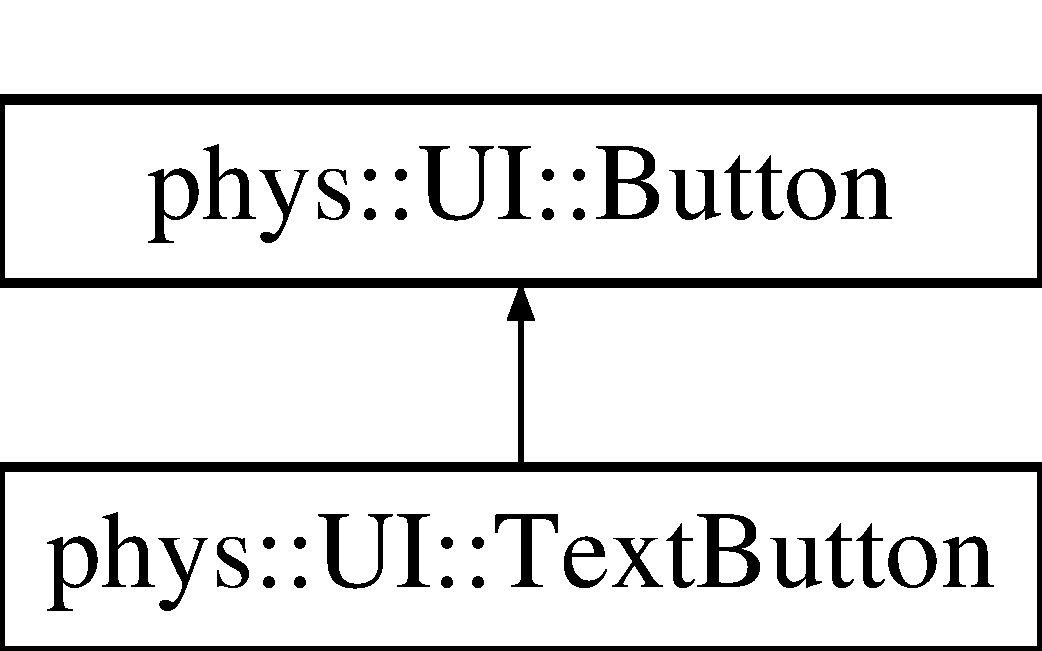
\includegraphics[height=2.000000cm]{classphys_1_1UI_1_1Button}
\end{center}
\end{figure}
\subsubsection*{Public Member Functions}
\begin{DoxyCompactItemize}
\item 
virtual void \hyperlink{classphys_1_1UI_1_1Button_a3b51fa981fdf869240bff082bafb56a9}{BindActivationKeyOrButton} (const \hyperlink{classphys_1_1MetaCode_a3e501cbb5bf0f6f1fdb7211465bda8d8}{MetaCode::InputCode} \&Code)
\begin{DoxyCompactList}\small\item\em Registers a keyboard key or mouse button that can activate this button. \item\end{DoxyCompactList}\item 
\hyperlink{classphys_1_1UI_1_1Button_a42ae60edce5a262254e4608a3ed9fc3c}{Button} (\hyperlink{namespacephys_a5ce5049f8b4bf88d6413c47b504ebb31}{ConstString} \&name, const \hyperlink{structphys_1_1UI_1_1RenderableRect}{RenderableRect} \&Rect, \hyperlink{classphys_1_1UI_1_1Layer}{Layer} $\ast$PLayer)
\begin{DoxyCompactList}\small\item\em Internal constructor. \item\end{DoxyCompactList}\item 
virtual bool \hyperlink{classphys_1_1UI_1_1Button_a72d76501d15053e3fbd9e7eb933e22de}{CheckMouseHover} ()
\begin{DoxyCompactList}\small\item\em Determines whether the mouse is over this button. \item\end{DoxyCompactList}\item 
virtual void \hyperlink{classphys_1_1UI_1_1Button_a8524260064c118597de5c18175f56493}{EnableMultipleActivations} (bool Enable)
\begin{DoxyCompactList}\small\item\em Enables or disables whether or not the button should be allowed to activate multiple times per frame. \item\end{DoxyCompactList}\item 
virtual void \hyperlink{classphys_1_1UI_1_1Button_a4fe6560484f1d78b08c96eaf967404d2}{EnableUserSprite} (bool Enable)
\begin{DoxyCompactList}\small\item\em Enables(or disables) the currently set User sprite. \item\end{DoxyCompactList}\item 
virtual UI::ActivationCondition \hyperlink{classphys_1_1UI_1_1Button_a193f5fa1554d978a5061c08bd4eca86b}{GetActivationCondition} ()
\begin{DoxyCompactList}\small\item\em Gets the condition for activation for this button. \item\end{DoxyCompactList}\item 
virtual \hyperlink{classphys_1_1Vector2}{Vector2} \hyperlink{classphys_1_1UI_1_1Button_a0b991ada87707d8d951dae7c0e3246f6}{GetActualPosition} ()
\begin{DoxyCompactList}\small\item\em Gets the top left position of this button in pixels. \item\end{DoxyCompactList}\item 
virtual \hyperlink{classphys_1_1Vector2}{Vector2} \hyperlink{classphys_1_1UI_1_1Button_ab6640af433afe96d5f6bd7016986d73f}{GetActualSize} ()
\begin{DoxyCompactList}\small\item\em Gets the size of this button in pixels. \item\end{DoxyCompactList}\item 
virtual std::vector$<$ \hyperlink{classphys_1_1MetaCode_a3e501cbb5bf0f6f1fdb7211465bda8d8}{MetaCode::InputCode} $>$ $\ast$ \hyperlink{classphys_1_1UI_1_1Button_adb1a79145196e9682261f18fa8de04fe}{GetKeyboardActivationKeys} ()
\begin{DoxyCompactList}\small\item\em Gets a vector with all the keyboard input codes used to activate this button. \item\end{DoxyCompactList}\item 
virtual std::vector$<$ \hyperlink{classphys_1_1MetaCode_a3e501cbb5bf0f6f1fdb7211465bda8d8}{MetaCode::InputCode} $>$ $\ast$ \hyperlink{classphys_1_1UI_1_1Button_a2256e2f15cf3aea5abd3279178dc3199}{GetMouseActivationButtons} ()
\begin{DoxyCompactList}\small\item\em Gets a vector with all the mouse input codes used to activate this button. \item\end{DoxyCompactList}\item 
virtual bool \hyperlink{classphys_1_1UI_1_1Button_a66522ebf5f3c75e96a6dfd99700a0f74}{GetMouseHover} ()
\begin{DoxyCompactList}\small\item\em Gets the stored value of whether or not the mouse is over the button. \item\end{DoxyCompactList}\item 
virtual \hyperlink{namespacephys_a5ce5049f8b4bf88d6413c47b504ebb31}{ConstString} \& \hyperlink{classphys_1_1UI_1_1Button_a1b757862cd1f4935d62c05ef4596b8a0}{GetName} ()
\begin{DoxyCompactList}\small\item\em Gets the name of this button. \item\end{DoxyCompactList}\item 
virtual \hyperlink{classphys_1_1Vector2}{Vector2} \hyperlink{classphys_1_1UI_1_1Button_adfa08ace813b88cae114e18f88942642}{GetPosition} ()
\begin{DoxyCompactList}\small\item\em Gets the relative top left position of this button. \item\end{DoxyCompactList}\item 
virtual \hyperlink{namespacephys_aa03900411993de7fbfec4789bc1d392e}{String} \hyperlink{classphys_1_1UI_1_1Button_a8aad3cb0e33a2bfc4fc4913bf19396a5}{GetPrimaryAtlas} ()
\begin{DoxyCompactList}\small\item\em Gets the currently set primary atlas. \item\end{DoxyCompactList}\item 
virtual UI::RenderPriority \hyperlink{classphys_1_1UI_1_1Button_aa17ffbc9b0d4eed151ff5ecbf93d88b8}{GetRenderPriority} ()
\begin{DoxyCompactList}\small\item\em Gets the priority this button should be rendered with. \item\end{DoxyCompactList}\item 
virtual \hyperlink{classphys_1_1Vector2}{Vector2} \hyperlink{classphys_1_1UI_1_1Button_ade75e042d1a19be5d4fb1b16913af5a5}{GetSize} ()
\begin{DoxyCompactList}\small\item\em Gets the relative size of this button. \item\end{DoxyCompactList}\item 
\hypertarget{classphys_1_1UI_1_1Button_a5a68803daf10281a85b4db1d4c18e412}{
virtual void \hyperlink{classphys_1_1UI_1_1Button_a5a68803daf10281a85b4db1d4c18e412}{Hide} ()}
\label{classphys_1_1UI_1_1Button_a5a68803daf10281a85b4db1d4c18e412}

\begin{DoxyCompactList}\small\item\em Forces this button to hide. \item\end{DoxyCompactList}\item 
virtual bool \hyperlink{classphys_1_1UI_1_1Button_ac54dde0e137f207bdec9a14b58063a6d}{IsActivated} ()
\begin{DoxyCompactList}\small\item\em Gets whether or not this button is currently activated. \item\end{DoxyCompactList}\item 
virtual bool \hyperlink{classphys_1_1UI_1_1Button_a6630a0e94a3998f6972b35a4e368b3ff}{IsMultipleActivationsEnabled} ()
\begin{DoxyCompactList}\small\item\em Gets whether or not multiple activations per frame are enabled for this button. \item\end{DoxyCompactList}\item 
virtual bool \hyperlink{classphys_1_1UI_1_1Button_a9c575f6433a5a455dc8c5de73d37839c}{IsTextButton} ()
\begin{DoxyCompactList}\small\item\em Gets whether this is a text button. \item\end{DoxyCompactList}\item 
virtual bool \hyperlink{classphys_1_1UI_1_1Button_a2bca8ace690157fa2646bcf1cb54397a}{IsVisible} ()
\begin{DoxyCompactList}\small\item\em Gets the visibility of this button. \item\end{DoxyCompactList}\item 
\hypertarget{classphys_1_1UI_1_1Button_adaf3f9ed9f8478e180278b71cb355db6}{
virtual void \hyperlink{classphys_1_1UI_1_1Button_adaf3f9ed9f8478e180278b71cb355db6}{NoBorder} ()}
\label{classphys_1_1UI_1_1Button_adaf3f9ed9f8478e180278b71cb355db6}

\begin{DoxyCompactList}\small\item\em Disables any border set on this rectangle if one is currently set. \item\end{DoxyCompactList}\item 
virtual void \hyperlink{classphys_1_1UI_1_1Button_ae875686ae568fc121eef980b24949cc1}{SetActivation} (bool Activate)
\begin{DoxyCompactList}\small\item\em Sets the button as activated, also calling any set callbacks. \item\end{DoxyCompactList}\item 
virtual void \hyperlink{classphys_1_1UI_1_1Button_a888cafb544472bbe3c5b023f4279030e}{SetActivationCondition} (const UI::ActivationCondition \&Condition)
\begin{DoxyCompactList}\small\item\em Sets the condition for activation for this button. \item\end{DoxyCompactList}\item 
virtual void \hyperlink{classphys_1_1UI_1_1Button_a50f175a9a9002b3270edc74154d4255b}{SetActualPosition} (const \hyperlink{classphys_1_1Vector2}{Vector2} \&Position)
\begin{DoxyCompactList}\small\item\em Sets the top left position of this button in pixels. \item\end{DoxyCompactList}\item 
virtual void \hyperlink{classphys_1_1UI_1_1Button_ab6c806b1bef7d1a3b9455914a1e9c8c0}{SetActualSize} (const \hyperlink{classphys_1_1Vector2}{Vector2} \&Size)
\begin{DoxyCompactList}\small\item\em Sets the size of this button in pixels. \item\end{DoxyCompactList}\item 
virtual void \hyperlink{classphys_1_1UI_1_1Button_a390aa5a409361507b5802141380bc1d3}{SetBackgroundColour} (const \hyperlink{classphys_1_1ColourValue}{ColourValue} \&Colour)
\begin{DoxyCompactList}\small\item\em Sets the background colour of the button. \item\end{DoxyCompactList}\item 
virtual void \hyperlink{classphys_1_1UI_1_1Button_a7cecb219a59fb55db6ac0070359bb23f}{SetBackgroundSprite} (const \hyperlink{namespacephys_aa03900411993de7fbfec4789bc1d392e}{String} \&Name)
\begin{DoxyCompactList}\small\item\em Sets the background image(if provided in the atlas) of the button. \item\end{DoxyCompactList}\item 
virtual void \hyperlink{classphys_1_1UI_1_1Button_a13899540adb0b039fec892f24a312686}{SetBackgroundSprite} (const \hyperlink{namespacephys_aa03900411993de7fbfec4789bc1d392e}{String} \&Name, const \hyperlink{namespacephys_aa03900411993de7fbfec4789bc1d392e}{String} \&Atlas)
\begin{DoxyCompactList}\small\item\em Sets the background image(if provided in the atlas) of the button from another atlas then the one currently set. \item\end{DoxyCompactList}\item 
virtual void \hyperlink{classphys_1_1UI_1_1Button_a8e7fa03ebbdf0c71dc60e5b95635894c}{SetBorder} (const \hyperlink{namespacephys_af7eb897198d265b8e868f45240230d5f}{Real} \&Width, const \hyperlink{classphys_1_1ColourValue}{ColourValue} \&Colour)
\begin{DoxyCompactList}\small\item\em Enables a border and sets it's colour. \item\end{DoxyCompactList}\item 
virtual void \hyperlink{classphys_1_1UI_1_1Button_aa9f8c1e2e91e22405bacd298c88eb845}{SetButtonCallback} (\hyperlink{classphys_1_1UI_1_1ButtonCallback}{ButtonCallback} $\ast$Call)
\begin{DoxyCompactList}\small\item\em Sets the callback for this button. See the \hyperlink{classphys_1_1UI_1_1ButtonCallback}{ButtonCallback} class for more info. \item\end{DoxyCompactList}\item 
virtual void \hyperlink{classphys_1_1UI_1_1Button_abf5f5997d71829bd7902139932a4b26b}{SetHoveredSprite} (const \hyperlink{namespacephys_aa03900411993de7fbfec4789bc1d392e}{String} \&Name, const \hyperlink{namespacephys_aa03900411993de7fbfec4789bc1d392e}{String} \&Atlas)
\begin{DoxyCompactList}\small\item\em Sets an alternate background image that will be applied when the mouse is over this button from another atlas then the one currently set. \item\end{DoxyCompactList}\item 
virtual void \hyperlink{classphys_1_1UI_1_1Button_a12cfac0dcc6324694f29968c0ca25d03}{SetHoveredSprite} (const \hyperlink{namespacephys_aa03900411993de7fbfec4789bc1d392e}{String} \&Name)
\begin{DoxyCompactList}\small\item\em Sets an alternate background image that will be applied when the mouse is over this button. \item\end{DoxyCompactList}\item 
virtual void \hyperlink{classphys_1_1UI_1_1Button_a68e1d9043a614e152c514a959be07d8c}{SetPosition} (const \hyperlink{classphys_1_1Vector2}{Vector2} \&Position)
\begin{DoxyCompactList}\small\item\em Sets the relative top left position of this button. \item\end{DoxyCompactList}\item 
virtual void \hyperlink{classphys_1_1UI_1_1Button_a23bea9f25eabd941f859208e39735b5b}{SetPrimaryAtlas} (const \hyperlink{namespacephys_aa03900411993de7fbfec4789bc1d392e}{String} \&Atlas)
\begin{DoxyCompactList}\small\item\em Sets the Atlas to be assumed when one isn't provided for atlas related tasks. \item\end{DoxyCompactList}\item 
virtual void \hyperlink{classphys_1_1UI_1_1Button_ad3e723b07cfdc73db7276d0339d15f38}{SetRenderPriority} (const UI::RenderPriority \&Priority)
\begin{DoxyCompactList}\small\item\em Sets the priority this button should be rendered with. \item\end{DoxyCompactList}\item 
virtual void \hyperlink{classphys_1_1UI_1_1Button_a956fe6caf82304cf1332a62b51b6b5de}{SetSize} (const \hyperlink{classphys_1_1Vector2}{Vector2} \&Size)
\begin{DoxyCompactList}\small\item\em Sets the relative size of this button. \item\end{DoxyCompactList}\item 
virtual void \hyperlink{classphys_1_1UI_1_1Button_aeb5ec136d8f307c5380c407f066b2ac1}{SetUserSprite} (const \hyperlink{namespacephys_aa03900411993de7fbfec4789bc1d392e}{String} \&Name, const \hyperlink{namespacephys_aa03900411993de7fbfec4789bc1d392e}{String} \&Atlas)
\begin{DoxyCompactList}\small\item\em Sets an alternate background image that is stored and can be quickly swapped with the active sprite from another atlas then the one currently set. \item\end{DoxyCompactList}\item 
virtual void \hyperlink{classphys_1_1UI_1_1Button_a8c3a5657daf79a882f71691e91785d4d}{SetUserSprite} (const \hyperlink{namespacephys_aa03900411993de7fbfec4789bc1d392e}{String} \&Name)
\begin{DoxyCompactList}\small\item\em Sets an alternate background image that is stored and can be quickly swapped with the active sprite. \item\end{DoxyCompactList}\item 
virtual void \hyperlink{classphys_1_1UI_1_1Button_a293a0a5296778fb3d638c31c5d9d4c75}{SetVisible} (bool Visible)
\begin{DoxyCompactList}\small\item\em Sets the visibility of this button. \item\end{DoxyCompactList}\item 
\hypertarget{classphys_1_1UI_1_1Button_aad25b9ec4b9c7cc232d419dcd68f420e}{
virtual void \hyperlink{classphys_1_1UI_1_1Button_aad25b9ec4b9c7cc232d419dcd68f420e}{Show} ()}
\label{classphys_1_1UI_1_1Button_aad25b9ec4b9c7cc232d419dcd68f420e}

\begin{DoxyCompactList}\small\item\em Forces this button to be shown. \item\end{DoxyCompactList}\item 
virtual void \hyperlink{classphys_1_1UI_1_1Button_a18f51eeb5685ed858b8842f65d566102}{UnbindActivationKeyOrButton} (const \hyperlink{classphys_1_1MetaCode_a3e501cbb5bf0f6f1fdb7211465bda8d8}{MetaCode::InputCode} \&Code)
\begin{DoxyCompactList}\small\item\em Removes a previously registered activation key or button. \item\end{DoxyCompactList}\item 
\hypertarget{classphys_1_1UI_1_1Button_a6b1a993ca1b4050e3741a77f0f1643df}{
virtual void \hyperlink{classphys_1_1UI_1_1Button_a6b1a993ca1b4050e3741a77f0f1643df}{UnbindAllActivationKeysAndButtons} ()}
\label{classphys_1_1UI_1_1Button_a6b1a993ca1b4050e3741a77f0f1643df}

\begin{DoxyCompactList}\small\item\em Clears all keyboard and mouse input codes from the list of activators. \item\end{DoxyCompactList}\item 
\hypertarget{classphys_1_1UI_1_1Button_a76b52d72810865ab05a6423a60894d50}{
virtual void \hyperlink{classphys_1_1UI_1_1Button_a76b52d72810865ab05a6423a60894d50}{UnbindAllKeyboardActivationKeys} ()}
\label{classphys_1_1UI_1_1Button_a76b52d72810865ab05a6423a60894d50}

\begin{DoxyCompactList}\small\item\em Clears all keyboard input codes from the list of activation keys. \item\end{DoxyCompactList}\item 
\hypertarget{classphys_1_1UI_1_1Button_ac1e6ed278f41bc49329e1fc1e445699c}{
virtual void \hyperlink{classphys_1_1UI_1_1Button_ac1e6ed278f41bc49329e1fc1e445699c}{UnbindAllMouseActivationButtons} ()}
\label{classphys_1_1UI_1_1Button_ac1e6ed278f41bc49329e1fc1e445699c}

\begin{DoxyCompactList}\small\item\em Clears all mouse input codes from the list of activation buttons. \item\end{DoxyCompactList}\item 
virtual void \hyperlink{classphys_1_1UI_1_1Button_ae69604605a9b4de08dbaf6738a241bb6}{UpdateDimensions} ()
\begin{DoxyCompactList}\small\item\em Updates the dimensions of this button to match those of the new screen size. \item\end{DoxyCompactList}\item 
\hypertarget{classphys_1_1UI_1_1Button_a80c8c92ae289e3161dde94bf1a5de59e}{
virtual \hyperlink{classphys_1_1UI_1_1Button_a80c8c92ae289e3161dde94bf1a5de59e}{$\sim$Button} ()}
\label{classphys_1_1UI_1_1Button_a80c8c92ae289e3161dde94bf1a5de59e}

\begin{DoxyCompactList}\small\item\em Class destructor. \item\end{DoxyCompactList}\end{DoxyCompactItemize}
\subsubsection*{Protected Member Functions}
\begin{DoxyCompactItemize}
\item 
\hypertarget{classphys_1_1UI_1_1Button_a83bf58f1a849d878265cd0cb8193ddf7}{
void {\bfseries SetHovered} (bool Hovered)}
\label{classphys_1_1UI_1_1Button_a83bf58f1a849d878265cd0cb8193ddf7}

\end{DoxyCompactItemize}
\subsubsection*{Protected Attributes}
\begin{DoxyCompactItemize}
\item 
\hypertarget{classphys_1_1UI_1_1Button_a659d498ea38854038a3ed487b24bd331}{
UI::ActivationCondition {\bfseries ActCond}}
\label{classphys_1_1UI_1_1Button_a659d498ea38854038a3ed487b24bd331}

\item 
\hypertarget{classphys_1_1UI_1_1Button_a7f4ee543e998a4bd369f05b531b1a04e}{
bool {\bfseries Activated}}
\label{classphys_1_1UI_1_1Button_a7f4ee543e998a4bd369f05b531b1a04e}

\item 
\hypertarget{classphys_1_1UI_1_1Button_a56fd3cc8871d0c112bcb46dcd7d59aed}{
\hyperlink{classphys_1_1UI_1_1ButtonCallback}{ButtonCallback} $\ast$ {\bfseries Callback}}
\label{classphys_1_1UI_1_1Button_a56fd3cc8871d0c112bcb46dcd7d59aed}

\item 
\hypertarget{classphys_1_1UI_1_1Button_ae58fc40169b6fb2acc06db63dcbff953}{
Gorilla::Rectangle $\ast$ {\bfseries GorillaRectangle}}
\label{classphys_1_1UI_1_1Button_ae58fc40169b6fb2acc06db63dcbff953}

\item 
\hypertarget{classphys_1_1UI_1_1Button_ab5d48f6d336d35645ffcc3061c0bcc48}{
Gorilla::Sprite $\ast$ {\bfseries HoveredSprite}}
\label{classphys_1_1UI_1_1Button_ab5d48f6d336d35645ffcc3061c0bcc48}

\item 
\hypertarget{classphys_1_1UI_1_1Button_ae5df151f265267d289adc904bfff5833}{
std::vector$<$ \hyperlink{classphys_1_1MetaCode_a3e501cbb5bf0f6f1fdb7211465bda8d8}{MetaCode::InputCode} $>$ {\bfseries KeyboardActivationKeys}}
\label{classphys_1_1UI_1_1Button_ae5df151f265267d289adc904bfff5833}

\item 
\hypertarget{classphys_1_1UI_1_1Button_ad98260c77b904ec926a2acc47268c16c}{
\hyperlink{classphys_1_1UIManager}{UIManager} $\ast$ {\bfseries Manager}}
\label{classphys_1_1UI_1_1Button_ad98260c77b904ec926a2acc47268c16c}

\item 
\hypertarget{classphys_1_1UI_1_1Button_af0ec4864f55387a715cc4cccd76676c8}{
std::vector$<$ \hyperlink{classphys_1_1MetaCode_a3e501cbb5bf0f6f1fdb7211465bda8d8}{MetaCode::InputCode} $>$ {\bfseries MouseActivationButtons}}
\label{classphys_1_1UI_1_1Button_af0ec4864f55387a715cc4cccd76676c8}

\item 
\hypertarget{classphys_1_1UI_1_1Button_a021052f6c6632623dfdf89bdc8ad8ec4}{
bool {\bfseries MouseHover}}
\label{classphys_1_1UI_1_1Button_a021052f6c6632623dfdf89bdc8ad8ec4}

\item 
\hypertarget{classphys_1_1UI_1_1Button_af33ffe0a2d4c4e5344e810c313a06e6f}{
bool {\bfseries MultipleActivations}}
\label{classphys_1_1UI_1_1Button_af33ffe0a2d4c4e5344e810c313a06e6f}

\item 
\hypertarget{classphys_1_1UI_1_1Button_ab3151f18855c8de2ffb80975f04041c1}{
\hyperlink{namespacephys_aa03900411993de7fbfec4789bc1d392e}{String} {\bfseries Name}}
\label{classphys_1_1UI_1_1Button_ab3151f18855c8de2ffb80975f04041c1}

\item 
\hypertarget{classphys_1_1UI_1_1Button_a4d6914524ef1d6c0248fee2c31bdb86a}{
Gorilla::Sprite $\ast$ {\bfseries NormalSprite}}
\label{classphys_1_1UI_1_1Button_a4d6914524ef1d6c0248fee2c31bdb86a}

\item 
\hypertarget{classphys_1_1UI_1_1Button_a611bab3af086add9cbc7a138e97af3b0}{
\hyperlink{classphys_1_1UI_1_1Layer}{Layer} $\ast$ {\bfseries Parent}}
\label{classphys_1_1UI_1_1Button_a611bab3af086add9cbc7a138e97af3b0}

\item 
\hypertarget{classphys_1_1UI_1_1Button_a981baa14d909cd6750553e3802545380}{
\hyperlink{classphys_1_1Vector2}{Vector2} {\bfseries RelPosition}}
\label{classphys_1_1UI_1_1Button_a981baa14d909cd6750553e3802545380}

\item 
\hypertarget{classphys_1_1UI_1_1Button_a413a4e4c3b815275051a881b7539a8f9}{
\hyperlink{classphys_1_1Vector2}{Vector2} {\bfseries RelSize}}
\label{classphys_1_1UI_1_1Button_a413a4e4c3b815275051a881b7539a8f9}

\item 
\hypertarget{classphys_1_1UI_1_1Button_afa82b63c5997cb9ec9dce3071048a556}{
Gorilla::Sprite $\ast$ {\bfseries UserSprite}}
\label{classphys_1_1UI_1_1Button_afa82b63c5997cb9ec9dce3071048a556}

\end{DoxyCompactItemize}


\subsubsection{Detailed Description}
This class is a helper class, specifically for use as a button. Unlike rectangles and captions, this class can be interacted with by clicking. It is important to understand what you want your space to do when selecting the class to use. 

Definition at line 72 of file uibutton.h.



\subsubsection{Constructor \& Destructor Documentation}
\hypertarget{classphys_1_1UI_1_1Button_a42ae60edce5a262254e4608a3ed9fc3c}{
\index{phys::UI::Button@{phys::UI::Button}!Button@{Button}}
\index{Button@{Button}!phys::UI::Button@{phys::UI::Button}}
\paragraph[{Button}]{\setlength{\rightskip}{0pt plus 5cm}phys::UI::Button::Button (
\begin{DoxyParamCaption}
\item[{{\bf ConstString} \&}]{name, }
\item[{const {\bf RenderableRect} \&}]{Rect, }
\item[{{\bf Layer} $\ast$}]{PLayer}
\end{DoxyParamCaption}
)}\hfill}
\label{classphys_1_1UI_1_1Button_a42ae60edce5a262254e4608a3ed9fc3c}


Internal constructor. 


\begin{DoxyParams}{Parameters}
{\em name} & The name of the button. \\
\hline
{\em Rect} & The Rect representing the position and size of the button. \\
\hline
{\em \hyperlink{classphys_1_1UI_1_1Layer}{Layer}} & Pointer to the \hyperlink{classphys_1_1UI_1_1Layer}{Layer} that created this button. \\
\hline
\end{DoxyParams}


Definition at line 56 of file uibutton.cpp.



\subsubsection{Member Function Documentation}
\hypertarget{classphys_1_1UI_1_1Button_a3b51fa981fdf869240bff082bafb56a9}{
\index{phys::UI::Button@{phys::UI::Button}!BindActivationKeyOrButton@{BindActivationKeyOrButton}}
\index{BindActivationKeyOrButton@{BindActivationKeyOrButton}!phys::UI::Button@{phys::UI::Button}}
\paragraph[{BindActivationKeyOrButton}]{\setlength{\rightskip}{0pt plus 5cm}void phys::UI::Button::BindActivationKeyOrButton (
\begin{DoxyParamCaption}
\item[{const {\bf MetaCode::InputCode} \&}]{Code}
\end{DoxyParamCaption}
)\hspace{0.3cm}{\ttfamily  \mbox{[}virtual\mbox{]}}}\hfill}
\label{classphys_1_1UI_1_1Button_a3b51fa981fdf869240bff082bafb56a9}


Registers a keyboard key or mouse button that can activate this button. 

In the case of a mouse button, the hover check has to return true to activate the button. 
\begin{DoxyParams}{Parameters}
{\em Code} & The input code to register that will trigger activation. \\
\hline
\end{DoxyParams}


\begin{Desc}
\item[\hyperlink{todo__todo000025}{Todo}]Throw an error? \end{Desc}




Definition at line 141 of file uibutton.cpp.

\hypertarget{classphys_1_1UI_1_1Button_a72d76501d15053e3fbd9e7eb933e22de}{
\index{phys::UI::Button@{phys::UI::Button}!CheckMouseHover@{CheckMouseHover}}
\index{CheckMouseHover@{CheckMouseHover}!phys::UI::Button@{phys::UI::Button}}
\paragraph[{CheckMouseHover}]{\setlength{\rightskip}{0pt plus 5cm}bool phys::UI::Button::CheckMouseHover (
\begin{DoxyParamCaption}
{}
\end{DoxyParamCaption}
)\hspace{0.3cm}{\ttfamily  \mbox{[}virtual\mbox{]}}}\hfill}
\label{classphys_1_1UI_1_1Button_a72d76501d15053e3fbd9e7eb933e22de}


Determines whether the mouse is over this button. 

While this can be called manually, it'll provide the same result if called more the once per frame. Currently the \hyperlink{classphys_1_1UIManager}{UIManager} calls this on it's own once per frame, so there isn't much point in calling this manually. \begin{DoxyReturn}{Returns}
Returns a bool indicating whether the mouse is over this button. 
\end{DoxyReturn}


Definition at line 241 of file uibutton.cpp.

\hypertarget{classphys_1_1UI_1_1Button_a8524260064c118597de5c18175f56493}{
\index{phys::UI::Button@{phys::UI::Button}!EnableMultipleActivations@{EnableMultipleActivations}}
\index{EnableMultipleActivations@{EnableMultipleActivations}!phys::UI::Button@{phys::UI::Button}}
\paragraph[{EnableMultipleActivations}]{\setlength{\rightskip}{0pt plus 5cm}void phys::UI::Button::EnableMultipleActivations (
\begin{DoxyParamCaption}
\item[{bool}]{Enable}
\end{DoxyParamCaption}
)\hspace{0.3cm}{\ttfamily  \mbox{[}virtual\mbox{]}}}\hfill}
\label{classphys_1_1UI_1_1Button_a8524260064c118597de5c18175f56493}


Enables or disables whether or not the button should be allowed to activate multiple times per frame. 

In most cases a button will only activate multiple times when using hotkeys, either when there are multiple keys hotkeyed to the same button, or when the mouse button is pressed over a UI button while a hotkey for it is activated in the same frame, or both. If you only want a UI element being triggered once per frame at most, you want this disabled. \par
 Default: false. 
\begin{DoxyParams}{Parameters}
{\em Enable} & Whether or not to enable this feature. \\
\hline
\end{DoxyParams}


Definition at line 231 of file uibutton.cpp.

\hypertarget{classphys_1_1UI_1_1Button_a4fe6560484f1d78b08c96eaf967404d2}{
\index{phys::UI::Button@{phys::UI::Button}!EnableUserSprite@{EnableUserSprite}}
\index{EnableUserSprite@{EnableUserSprite}!phys::UI::Button@{phys::UI::Button}}
\paragraph[{EnableUserSprite}]{\setlength{\rightskip}{0pt plus 5cm}void phys::UI::Button::EnableUserSprite (
\begin{DoxyParamCaption}
\item[{bool}]{Enable}
\end{DoxyParamCaption}
)\hspace{0.3cm}{\ttfamily  \mbox{[}virtual\mbox{]}}}\hfill}
\label{classphys_1_1UI_1_1Button_a4fe6560484f1d78b08c96eaf967404d2}


Enables(or disables) the currently set User sprite. 


\begin{DoxyParams}{Parameters}
{\em Enable} & If true, this will swap the current sprite with the user sprite, if false it will swap the User sprite for the normal sprite. \\
\hline
\end{DoxyParams}


Definition at line 300 of file uibutton.cpp.

\hypertarget{classphys_1_1UI_1_1Button_a193f5fa1554d978a5061c08bd4eca86b}{
\index{phys::UI::Button@{phys::UI::Button}!GetActivationCondition@{GetActivationCondition}}
\index{GetActivationCondition@{GetActivationCondition}!phys::UI::Button@{phys::UI::Button}}
\paragraph[{GetActivationCondition}]{\setlength{\rightskip}{0pt plus 5cm}UI::ActivationCondition phys::UI::Button::GetActivationCondition (
\begin{DoxyParamCaption}
{}
\end{DoxyParamCaption}
)\hspace{0.3cm}{\ttfamily  \mbox{[}virtual\mbox{]}}}\hfill}
\label{classphys_1_1UI_1_1Button_a193f5fa1554d978a5061c08bd4eca86b}


Gets the condition for activation for this button. 

See the ActivationCondition enum for more details. \begin{DoxyReturn}{Returns}
Returns an enum value indicating the condition for activation for this button. 
\end{DoxyReturn}


Definition at line 212 of file uibutton.cpp.

\hypertarget{classphys_1_1UI_1_1Button_a0b991ada87707d8d951dae7c0e3246f6}{
\index{phys::UI::Button@{phys::UI::Button}!GetActualPosition@{GetActualPosition}}
\index{GetActualPosition@{GetActualPosition}!phys::UI::Button@{phys::UI::Button}}
\paragraph[{GetActualPosition}]{\setlength{\rightskip}{0pt plus 5cm}{\bf Vector2} phys::UI::Button::GetActualPosition (
\begin{DoxyParamCaption}
{}
\end{DoxyParamCaption}
)\hspace{0.3cm}{\ttfamily  \mbox{[}virtual\mbox{]}}}\hfill}
\label{classphys_1_1UI_1_1Button_a0b991ada87707d8d951dae7c0e3246f6}


Gets the top left position of this button in pixels. 

\begin{DoxyReturn}{Returns}
Returns a \hyperlink{classphys_1_1Vector2}{Vector2} representing the location of this button. 
\end{DoxyReturn}


Reimplemented in \hyperlink{classphys_1_1UI_1_1TextButton_ab406bec58bf6244c3e867fefd19d4d7f}{phys::UI::TextButton}.



Definition at line 340 of file uibutton.cpp.

\hypertarget{classphys_1_1UI_1_1Button_ab6640af433afe96d5f6bd7016986d73f}{
\index{phys::UI::Button@{phys::UI::Button}!GetActualSize@{GetActualSize}}
\index{GetActualSize@{GetActualSize}!phys::UI::Button@{phys::UI::Button}}
\paragraph[{GetActualSize}]{\setlength{\rightskip}{0pt plus 5cm}{\bf Vector2} phys::UI::Button::GetActualSize (
\begin{DoxyParamCaption}
{}
\end{DoxyParamCaption}
)\hspace{0.3cm}{\ttfamily  \mbox{[}virtual\mbox{]}}}\hfill}
\label{classphys_1_1UI_1_1Button_ab6640af433afe96d5f6bd7016986d73f}


Gets the size of this button in pixels. 

\begin{DoxyReturn}{Returns}
Returns a vector2 representing the size of this button. 
\end{DoxyReturn}


Reimplemented in \hyperlink{classphys_1_1UI_1_1TextButton_a062b31c199f875d4f825f6be1d11fb55}{phys::UI::TextButton}.



Definition at line 366 of file uibutton.cpp.

\hypertarget{classphys_1_1UI_1_1Button_adb1a79145196e9682261f18fa8de04fe}{
\index{phys::UI::Button@{phys::UI::Button}!GetKeyboardActivationKeys@{GetKeyboardActivationKeys}}
\index{GetKeyboardActivationKeys@{GetKeyboardActivationKeys}!phys::UI::Button@{phys::UI::Button}}
\paragraph[{GetKeyboardActivationKeys}]{\setlength{\rightskip}{0pt plus 5cm}std::vector$<$ {\bf MetaCode::InputCode} $>$ $\ast$ phys::UI::Button::GetKeyboardActivationKeys (
\begin{DoxyParamCaption}
{}
\end{DoxyParamCaption}
)\hspace{0.3cm}{\ttfamily  \mbox{[}virtual\mbox{]}}}\hfill}
\label{classphys_1_1UI_1_1Button_adb1a79145196e9682261f18fa8de04fe}


Gets a vector with all the keyboard input codes used to activate this button. 

\begin{DoxyReturn}{Returns}
Returns a pointer to an std::vector containing all the keyboard keys that will activate this button. 
\end{DoxyReturn}


Definition at line 422 of file uibutton.cpp.

\hypertarget{classphys_1_1UI_1_1Button_a2256e2f15cf3aea5abd3279178dc3199}{
\index{phys::UI::Button@{phys::UI::Button}!GetMouseActivationButtons@{GetMouseActivationButtons}}
\index{GetMouseActivationButtons@{GetMouseActivationButtons}!phys::UI::Button@{phys::UI::Button}}
\paragraph[{GetMouseActivationButtons}]{\setlength{\rightskip}{0pt plus 5cm}std::vector$<$ {\bf MetaCode::InputCode} $>$ $\ast$ phys::UI::Button::GetMouseActivationButtons (
\begin{DoxyParamCaption}
{}
\end{DoxyParamCaption}
)\hspace{0.3cm}{\ttfamily  \mbox{[}virtual\mbox{]}}}\hfill}
\label{classphys_1_1UI_1_1Button_a2256e2f15cf3aea5abd3279178dc3199}


Gets a vector with all the mouse input codes used to activate this button. 

\begin{DoxyReturn}{Returns}
Returns a pointer to an std::vector containing all the mouse buttons that will activate this button. 
\end{DoxyReturn}


Definition at line 427 of file uibutton.cpp.

\hypertarget{classphys_1_1UI_1_1Button_a66522ebf5f3c75e96a6dfd99700a0f74}{
\index{phys::UI::Button@{phys::UI::Button}!GetMouseHover@{GetMouseHover}}
\index{GetMouseHover@{GetMouseHover}!phys::UI::Button@{phys::UI::Button}}
\paragraph[{GetMouseHover}]{\setlength{\rightskip}{0pt plus 5cm}bool phys::UI::Button::GetMouseHover (
\begin{DoxyParamCaption}
{}
\end{DoxyParamCaption}
)\hspace{0.3cm}{\ttfamily  \mbox{[}virtual\mbox{]}}}\hfill}
\label{classphys_1_1UI_1_1Button_a66522ebf5f3c75e96a6dfd99700a0f74}


Gets the stored value of whether or not the mouse is over the button. 

This function does not perform any checks. If you want to do a manual check, call \hyperlink{classphys_1_1UI_1_1Button_a72d76501d15053e3fbd9e7eb933e22de}{CheckMouseHover()}. \begin{DoxyReturn}{Returns}
Returns the stored value of whether or not the mouse is over the button. 
\end{DoxyReturn}


Definition at line 252 of file uibutton.cpp.

\hypertarget{classphys_1_1UI_1_1Button_a1b757862cd1f4935d62c05ef4596b8a0}{
\index{phys::UI::Button@{phys::UI::Button}!GetName@{GetName}}
\index{GetName@{GetName}!phys::UI::Button@{phys::UI::Button}}
\paragraph[{GetName}]{\setlength{\rightskip}{0pt plus 5cm}{\bf ConstString} \& phys::UI::Button::GetName (
\begin{DoxyParamCaption}
{}
\end{DoxyParamCaption}
)\hspace{0.3cm}{\ttfamily  \mbox{[}virtual\mbox{]}}}\hfill}
\label{classphys_1_1UI_1_1Button_a1b757862cd1f4935d62c05ef4596b8a0}


Gets the name of this button. 

\begin{DoxyReturn}{Returns}
Returns a string containing the name of this button. 
\end{DoxyReturn}


Definition at line 126 of file uibutton.cpp.

\hypertarget{classphys_1_1UI_1_1Button_adfa08ace813b88cae114e18f88942642}{
\index{phys::UI::Button@{phys::UI::Button}!GetPosition@{GetPosition}}
\index{GetPosition@{GetPosition}!phys::UI::Button@{phys::UI::Button}}
\paragraph[{GetPosition}]{\setlength{\rightskip}{0pt plus 5cm}{\bf Vector2} phys::UI::Button::GetPosition (
\begin{DoxyParamCaption}
{}
\end{DoxyParamCaption}
)\hspace{0.3cm}{\ttfamily  \mbox{[}virtual\mbox{]}}}\hfill}
\label{classphys_1_1UI_1_1Button_adfa08ace813b88cae114e18f88942642}


Gets the relative top left position of this button. 

\begin{DoxyReturn}{Returns}
Returns a \hyperlink{classphys_1_1Vector2}{Vector2} representing the location of this button. 
\end{DoxyReturn}


Reimplemented in \hyperlink{classphys_1_1UI_1_1TextButton_a09768e0666a109b7d35fd8b78240cfd3}{phys::UI::TextButton}.



Definition at line 328 of file uibutton.cpp.

\hypertarget{classphys_1_1UI_1_1Button_a8aad3cb0e33a2bfc4fc4913bf19396a5}{
\index{phys::UI::Button@{phys::UI::Button}!GetPrimaryAtlas@{GetPrimaryAtlas}}
\index{GetPrimaryAtlas@{GetPrimaryAtlas}!phys::UI::Button@{phys::UI::Button}}
\paragraph[{GetPrimaryAtlas}]{\setlength{\rightskip}{0pt plus 5cm}{\bf String} phys::UI::Button::GetPrimaryAtlas (
\begin{DoxyParamCaption}
{}
\end{DoxyParamCaption}
)\hspace{0.3cm}{\ttfamily  \mbox{[}virtual\mbox{]}}}\hfill}
\label{classphys_1_1UI_1_1Button_a8aad3cb0e33a2bfc4fc4913bf19396a5}


Gets the currently set primary atlas. 

\begin{DoxyReturn}{Returns}
Returns a string containing the name of the primary atlas that is set, or an empty string if none. 
\end{DoxyReturn}


Definition at line 417 of file uibutton.cpp.

\hypertarget{classphys_1_1UI_1_1Button_aa17ffbc9b0d4eed151ff5ecbf93d88b8}{
\index{phys::UI::Button@{phys::UI::Button}!GetRenderPriority@{GetRenderPriority}}
\index{GetRenderPriority@{GetRenderPriority}!phys::UI::Button@{phys::UI::Button}}
\paragraph[{GetRenderPriority}]{\setlength{\rightskip}{0pt plus 5cm}UI::RenderPriority phys::UI::Button::GetRenderPriority (
\begin{DoxyParamCaption}
{}
\end{DoxyParamCaption}
)\hspace{0.3cm}{\ttfamily  \mbox{[}virtual\mbox{]}}}\hfill}
\label{classphys_1_1UI_1_1Button_aa17ffbc9b0d4eed151ff5ecbf93d88b8}


Gets the priority this button should be rendered with. 

\begin{DoxyReturn}{Returns}
Returns an enum value representing this button's priority level. 
\end{DoxyReturn}


Reimplemented in \hyperlink{classphys_1_1UI_1_1TextButton_ad339621af6e73ff9702c0dd4cdadbb73}{phys::UI::TextButton}.



Definition at line 392 of file uibutton.cpp.

\hypertarget{classphys_1_1UI_1_1Button_ade75e042d1a19be5d4fb1b16913af5a5}{
\index{phys::UI::Button@{phys::UI::Button}!GetSize@{GetSize}}
\index{GetSize@{GetSize}!phys::UI::Button@{phys::UI::Button}}
\paragraph[{GetSize}]{\setlength{\rightskip}{0pt plus 5cm}{\bf Vector2} phys::UI::Button::GetSize (
\begin{DoxyParamCaption}
{}
\end{DoxyParamCaption}
)\hspace{0.3cm}{\ttfamily  \mbox{[}virtual\mbox{]}}}\hfill}
\label{classphys_1_1UI_1_1Button_ade75e042d1a19be5d4fb1b16913af5a5}


Gets the relative size of this button. 

\begin{DoxyReturn}{Returns}
Returns a vector2 representing the size of this button. 
\end{DoxyReturn}


Reimplemented in \hyperlink{classphys_1_1UI_1_1TextButton_a21f1ff24070711e5a42eae4eb54d02d6}{phys::UI::TextButton}.



Definition at line 354 of file uibutton.cpp.

\hypertarget{classphys_1_1UI_1_1Button_ac54dde0e137f207bdec9a14b58063a6d}{
\index{phys::UI::Button@{phys::UI::Button}!IsActivated@{IsActivated}}
\index{IsActivated@{IsActivated}!phys::UI::Button@{phys::UI::Button}}
\paragraph[{IsActivated}]{\setlength{\rightskip}{0pt plus 5cm}bool phys::UI::Button::IsActivated (
\begin{DoxyParamCaption}
{}
\end{DoxyParamCaption}
)\hspace{0.3cm}{\ttfamily  \mbox{[}virtual\mbox{]}}}\hfill}
\label{classphys_1_1UI_1_1Button_ac54dde0e137f207bdec9a14b58063a6d}


Gets whether or not this button is currently activated. 

\hyperlink{classphys_1_1UI_1_1Button}{Button} activations are cleared every frame by the UI manager. \begin{DoxyReturn}{Returns}
Returns whether or not this button has been activated. 
\end{DoxyReturn}


Definition at line 226 of file uibutton.cpp.

\hypertarget{classphys_1_1UI_1_1Button_a6630a0e94a3998f6972b35a4e368b3ff}{
\index{phys::UI::Button@{phys::UI::Button}!IsMultipleActivationsEnabled@{IsMultipleActivationsEnabled}}
\index{IsMultipleActivationsEnabled@{IsMultipleActivationsEnabled}!phys::UI::Button@{phys::UI::Button}}
\paragraph[{IsMultipleActivationsEnabled}]{\setlength{\rightskip}{0pt plus 5cm}bool phys::UI::Button::IsMultipleActivationsEnabled (
\begin{DoxyParamCaption}
{}
\end{DoxyParamCaption}
)\hspace{0.3cm}{\ttfamily  \mbox{[}virtual\mbox{]}}}\hfill}
\label{classphys_1_1UI_1_1Button_a6630a0e94a3998f6972b35a4e368b3ff}


Gets whether or not multiple activations per frame are enabled for this button. 

\begin{DoxyReturn}{Returns}
Returns a bool indicating whether or not multiple activations are allowed for this button. 
\end{DoxyReturn}


Definition at line 236 of file uibutton.cpp.

\hypertarget{classphys_1_1UI_1_1Button_a9c575f6433a5a455dc8c5de73d37839c}{
\index{phys::UI::Button@{phys::UI::Button}!IsTextButton@{IsTextButton}}
\index{IsTextButton@{IsTextButton}!phys::UI::Button@{phys::UI::Button}}
\paragraph[{IsTextButton}]{\setlength{\rightskip}{0pt plus 5cm}bool phys::UI::Button::IsTextButton (
\begin{DoxyParamCaption}
{}
\end{DoxyParamCaption}
)\hspace{0.3cm}{\ttfamily  \mbox{[}virtual\mbox{]}}}\hfill}
\label{classphys_1_1UI_1_1Button_a9c575f6433a5a455dc8c5de73d37839c}


Gets whether this is a text button. 

\begin{DoxyReturn}{Returns}
Returns a bool representing whether or not this is a text button. 
\end{DoxyReturn}


Reimplemented in \hyperlink{classphys_1_1UI_1_1TextButton_ad3d493189347077db92e609e47f837f5}{phys::UI::TextButton}.



Definition at line 131 of file uibutton.cpp.

\hypertarget{classphys_1_1UI_1_1Button_a2bca8ace690157fa2646bcf1cb54397a}{
\index{phys::UI::Button@{phys::UI::Button}!IsVisible@{IsVisible}}
\index{IsVisible@{IsVisible}!phys::UI::Button@{phys::UI::Button}}
\paragraph[{IsVisible}]{\setlength{\rightskip}{0pt plus 5cm}bool phys::UI::Button::IsVisible (
\begin{DoxyParamCaption}
{}
\end{DoxyParamCaption}
)\hspace{0.3cm}{\ttfamily  \mbox{[}virtual\mbox{]}}}\hfill}
\label{classphys_1_1UI_1_1Button_a2bca8ace690157fa2646bcf1cb54397a}


Gets the visibility of this button. 

\begin{DoxyReturn}{Returns}
Returns a bool representing the visibility of this button. 
\end{DoxyReturn}


Reimplemented in \hyperlink{classphys_1_1UI_1_1TextButton_a505167a00d343d704df1f759cd12ed1e}{phys::UI::TextButton}.



Definition at line 111 of file uibutton.cpp.

\hypertarget{classphys_1_1UI_1_1Button_ae875686ae568fc121eef980b24949cc1}{
\index{phys::UI::Button@{phys::UI::Button}!SetActivation@{SetActivation}}
\index{SetActivation@{SetActivation}!phys::UI::Button@{phys::UI::Button}}
\paragraph[{SetActivation}]{\setlength{\rightskip}{0pt plus 5cm}void phys::UI::Button::SetActivation (
\begin{DoxyParamCaption}
\item[{bool}]{Activate}
\end{DoxyParamCaption}
)\hspace{0.3cm}{\ttfamily  \mbox{[}virtual\mbox{]}}}\hfill}
\label{classphys_1_1UI_1_1Button_ae875686ae568fc121eef980b24949cc1}


Sets the button as activated, also calling any set callbacks. 

This shouldn't be called on manually unless you know exactly what you are doing. 
\begin{DoxyParams}{Parameters}
{\em Activate} & The state of activation to be applied. \\
\hline
\end{DoxyParams}


Definition at line 217 of file uibutton.cpp.

\hypertarget{classphys_1_1UI_1_1Button_a888cafb544472bbe3c5b023f4279030e}{
\index{phys::UI::Button@{phys::UI::Button}!SetActivationCondition@{SetActivationCondition}}
\index{SetActivationCondition@{SetActivationCondition}!phys::UI::Button@{phys::UI::Button}}
\paragraph[{SetActivationCondition}]{\setlength{\rightskip}{0pt plus 5cm}void phys::UI::Button::SetActivationCondition (
\begin{DoxyParamCaption}
\item[{const UI::ActivationCondition \&}]{Condition}
\end{DoxyParamCaption}
)\hspace{0.3cm}{\ttfamily  \mbox{[}virtual\mbox{]}}}\hfill}
\label{classphys_1_1UI_1_1Button_a888cafb544472bbe3c5b023f4279030e}


Sets the condition for activation for this button. 

See the ActivationCondition enum for more details. 
\begin{DoxyParams}{Parameters}
{\em Condition} & The condition to be set. \\
\hline
\end{DoxyParams}


Definition at line 207 of file uibutton.cpp.

\hypertarget{classphys_1_1UI_1_1Button_a50f175a9a9002b3270edc74154d4255b}{
\index{phys::UI::Button@{phys::UI::Button}!SetActualPosition@{SetActualPosition}}
\index{SetActualPosition@{SetActualPosition}!phys::UI::Button@{phys::UI::Button}}
\paragraph[{SetActualPosition}]{\setlength{\rightskip}{0pt plus 5cm}void phys::UI::Button::SetActualPosition (
\begin{DoxyParamCaption}
\item[{const {\bf Vector2} \&}]{Position}
\end{DoxyParamCaption}
)\hspace{0.3cm}{\ttfamily  \mbox{[}virtual\mbox{]}}}\hfill}
\label{classphys_1_1UI_1_1Button_a50f175a9a9002b3270edc74154d4255b}


Sets the top left position of this button in pixels. 


\begin{DoxyParams}{Parameters}
{\em Position} & A \hyperlink{classphys_1_1Vector2}{Vector2} representing the location of this button. \\
\hline
\end{DoxyParams}


Reimplemented in \hyperlink{classphys_1_1UI_1_1TextButton_aa82c174bba5db127a5a9977b9fdf1384}{phys::UI::TextButton}.



Definition at line 333 of file uibutton.cpp.

\hypertarget{classphys_1_1UI_1_1Button_ab6c806b1bef7d1a3b9455914a1e9c8c0}{
\index{phys::UI::Button@{phys::UI::Button}!SetActualSize@{SetActualSize}}
\index{SetActualSize@{SetActualSize}!phys::UI::Button@{phys::UI::Button}}
\paragraph[{SetActualSize}]{\setlength{\rightskip}{0pt plus 5cm}void phys::UI::Button::SetActualSize (
\begin{DoxyParamCaption}
\item[{const {\bf Vector2} \&}]{Size}
\end{DoxyParamCaption}
)\hspace{0.3cm}{\ttfamily  \mbox{[}virtual\mbox{]}}}\hfill}
\label{classphys_1_1UI_1_1Button_ab6c806b1bef7d1a3b9455914a1e9c8c0}


Sets the size of this button in pixels. 


\begin{DoxyParams}{Parameters}
{\em Size} & A vector2 representing the size of this button. \\
\hline
\end{DoxyParams}


Reimplemented in \hyperlink{classphys_1_1UI_1_1TextButton_a768d203a323cca2054fa355c25fab9ef}{phys::UI::TextButton}.



Definition at line 359 of file uibutton.cpp.

\hypertarget{classphys_1_1UI_1_1Button_a390aa5a409361507b5802141380bc1d3}{
\index{phys::UI::Button@{phys::UI::Button}!SetBackgroundColour@{SetBackgroundColour}}
\index{SetBackgroundColour@{SetBackgroundColour}!phys::UI::Button@{phys::UI::Button}}
\paragraph[{SetBackgroundColour}]{\setlength{\rightskip}{0pt plus 5cm}void phys::UI::Button::SetBackgroundColour (
\begin{DoxyParamCaption}
\item[{const {\bf ColourValue} \&}]{Colour}
\end{DoxyParamCaption}
)\hspace{0.3cm}{\ttfamily  \mbox{[}virtual\mbox{]}}}\hfill}
\label{classphys_1_1UI_1_1Button_a390aa5a409361507b5802141380bc1d3}


Sets the background colour of the button. 


\begin{DoxyParams}{Parameters}
{\em Colour} & A colour value representing the colour to be set. \\
\hline
\end{DoxyParams}


Definition at line 257 of file uibutton.cpp.

\hypertarget{classphys_1_1UI_1_1Button_a7cecb219a59fb55db6ac0070359bb23f}{
\index{phys::UI::Button@{phys::UI::Button}!SetBackgroundSprite@{SetBackgroundSprite}}
\index{SetBackgroundSprite@{SetBackgroundSprite}!phys::UI::Button@{phys::UI::Button}}
\paragraph[{SetBackgroundSprite}]{\setlength{\rightskip}{0pt plus 5cm}void phys::UI::Button::SetBackgroundSprite (
\begin{DoxyParamCaption}
\item[{const {\bf String} \&}]{Name}
\end{DoxyParamCaption}
)\hspace{0.3cm}{\ttfamily  \mbox{[}virtual\mbox{]}}}\hfill}
\label{classphys_1_1UI_1_1Button_a7cecb219a59fb55db6ac0070359bb23f}


Sets the background image(if provided in the atlas) of the button. 


\begin{DoxyParams}{Parameters}
{\em Name} & The name of the sprite to set as the background. \\
\hline
\end{DoxyParams}


Definition at line 262 of file uibutton.cpp.

\hypertarget{classphys_1_1UI_1_1Button_a13899540adb0b039fec892f24a312686}{
\index{phys::UI::Button@{phys::UI::Button}!SetBackgroundSprite@{SetBackgroundSprite}}
\index{SetBackgroundSprite@{SetBackgroundSprite}!phys::UI::Button@{phys::UI::Button}}
\paragraph[{SetBackgroundSprite}]{\setlength{\rightskip}{0pt plus 5cm}void phys::UI::Button::SetBackgroundSprite (
\begin{DoxyParamCaption}
\item[{const {\bf String} \&}]{Name, }
\item[{const {\bf String} \&}]{Atlas}
\end{DoxyParamCaption}
)\hspace{0.3cm}{\ttfamily  \mbox{[}virtual\mbox{]}}}\hfill}
\label{classphys_1_1UI_1_1Button_a13899540adb0b039fec892f24a312686}


Sets the background image(if provided in the atlas) of the button from another atlas then the one currently set. 


\begin{DoxyParams}{Parameters}
{\em Name} & The name of the sprite to set as the background. \\
\hline
{\em Atlas} & The Atlas to load the sprite from. \\
\hline
\end{DoxyParams}


Definition at line 269 of file uibutton.cpp.

\hypertarget{classphys_1_1UI_1_1Button_a8e7fa03ebbdf0c71dc60e5b95635894c}{
\index{phys::UI::Button@{phys::UI::Button}!SetBorder@{SetBorder}}
\index{SetBorder@{SetBorder}!phys::UI::Button@{phys::UI::Button}}
\paragraph[{SetBorder}]{\setlength{\rightskip}{0pt plus 5cm}void phys::UI::Button::SetBorder (
\begin{DoxyParamCaption}
\item[{const {\bf Real} \&}]{Width, }
\item[{const {\bf ColourValue} \&}]{Colour}
\end{DoxyParamCaption}
)\hspace{0.3cm}{\ttfamily  \mbox{[}virtual\mbox{]}}}\hfill}
\label{classphys_1_1UI_1_1Button_a8e7fa03ebbdf0c71dc60e5b95635894c}


Enables a border and sets it's colour. 


\begin{DoxyParams}{Parameters}
{\em Colour} & A colour value representing the colour to be set. \\
\hline
\end{DoxyParams}


Definition at line 310 of file uibutton.cpp.

\hypertarget{classphys_1_1UI_1_1Button_aa9f8c1e2e91e22405bacd298c88eb845}{
\index{phys::UI::Button@{phys::UI::Button}!SetButtonCallback@{SetButtonCallback}}
\index{SetButtonCallback@{SetButtonCallback}!phys::UI::Button@{phys::UI::Button}}
\paragraph[{SetButtonCallback}]{\setlength{\rightskip}{0pt plus 5cm}void phys::UI::Button::SetButtonCallback (
\begin{DoxyParamCaption}
\item[{{\bf ButtonCallback} $\ast$}]{Call}
\end{DoxyParamCaption}
)\hspace{0.3cm}{\ttfamily  \mbox{[}virtual\mbox{]}}}\hfill}
\label{classphys_1_1UI_1_1Button_aa9f8c1e2e91e22405bacd298c88eb845}


Sets the callback for this button. See the \hyperlink{classphys_1_1UI_1_1ButtonCallback}{ButtonCallback} class for more info. 

You can pass in a null pointer to disable a callback. 
\begin{DoxyParams}{Parameters}
{\em Call} & A pointer to the callback you wish to have set for this button. \\
\hline
\end{DoxyParams}


Definition at line 136 of file uibutton.cpp.

\hypertarget{classphys_1_1UI_1_1Button_a12cfac0dcc6324694f29968c0ca25d03}{
\index{phys::UI::Button@{phys::UI::Button}!SetHoveredSprite@{SetHoveredSprite}}
\index{SetHoveredSprite@{SetHoveredSprite}!phys::UI::Button@{phys::UI::Button}}
\paragraph[{SetHoveredSprite}]{\setlength{\rightskip}{0pt plus 5cm}void phys::UI::Button::SetHoveredSprite (
\begin{DoxyParamCaption}
\item[{const {\bf String} \&}]{Name}
\end{DoxyParamCaption}
)\hspace{0.3cm}{\ttfamily  \mbox{[}virtual\mbox{]}}}\hfill}
\label{classphys_1_1UI_1_1Button_a12cfac0dcc6324694f29968c0ca25d03}


Sets an alternate background image that will be applied when the mouse is over this button. 


\begin{DoxyParams}{Parameters}
{\em Name} & The name of the sprite to set as the alternate background. \\
\hline
\end{DoxyParams}


Definition at line 276 of file uibutton.cpp.

\hypertarget{classphys_1_1UI_1_1Button_abf5f5997d71829bd7902139932a4b26b}{
\index{phys::UI::Button@{phys::UI::Button}!SetHoveredSprite@{SetHoveredSprite}}
\index{SetHoveredSprite@{SetHoveredSprite}!phys::UI::Button@{phys::UI::Button}}
\paragraph[{SetHoveredSprite}]{\setlength{\rightskip}{0pt plus 5cm}void phys::UI::Button::SetHoveredSprite (
\begin{DoxyParamCaption}
\item[{const {\bf String} \&}]{Name, }
\item[{const {\bf String} \&}]{Atlas}
\end{DoxyParamCaption}
)\hspace{0.3cm}{\ttfamily  \mbox{[}virtual\mbox{]}}}\hfill}
\label{classphys_1_1UI_1_1Button_abf5f5997d71829bd7902139932a4b26b}


Sets an alternate background image that will be applied when the mouse is over this button from another atlas then the one currently set. 


\begin{DoxyParams}{Parameters}
{\em Name} & The name of the sprite to set as the alternate background. \\
\hline
{\em Atlas} & The Atlas to load the sprite from. \\
\hline
\end{DoxyParams}


Definition at line 282 of file uibutton.cpp.

\hypertarget{classphys_1_1UI_1_1Button_a68e1d9043a614e152c514a959be07d8c}{
\index{phys::UI::Button@{phys::UI::Button}!SetPosition@{SetPosition}}
\index{SetPosition@{SetPosition}!phys::UI::Button@{phys::UI::Button}}
\paragraph[{SetPosition}]{\setlength{\rightskip}{0pt plus 5cm}void phys::UI::Button::SetPosition (
\begin{DoxyParamCaption}
\item[{const {\bf Vector2} \&}]{Position}
\end{DoxyParamCaption}
)\hspace{0.3cm}{\ttfamily  \mbox{[}virtual\mbox{]}}}\hfill}
\label{classphys_1_1UI_1_1Button_a68e1d9043a614e152c514a959be07d8c}


Sets the relative top left position of this button. 


\begin{DoxyParams}{Parameters}
{\em Position} & A \hyperlink{classphys_1_1Vector2}{Vector2} representing the location of this button. \\
\hline
\end{DoxyParams}


Reimplemented in \hyperlink{classphys_1_1UI_1_1TextButton_a52230b17c81743438bc0cd08eb49a5c5}{phys::UI::TextButton}.



Definition at line 320 of file uibutton.cpp.

\hypertarget{classphys_1_1UI_1_1Button_a23bea9f25eabd941f859208e39735b5b}{
\index{phys::UI::Button@{phys::UI::Button}!SetPrimaryAtlas@{SetPrimaryAtlas}}
\index{SetPrimaryAtlas@{SetPrimaryAtlas}!phys::UI::Button@{phys::UI::Button}}
\paragraph[{SetPrimaryAtlas}]{\setlength{\rightskip}{0pt plus 5cm}void phys::UI::Button::SetPrimaryAtlas (
\begin{DoxyParamCaption}
\item[{const {\bf String} \&}]{Atlas}
\end{DoxyParamCaption}
)\hspace{0.3cm}{\ttfamily  \mbox{[}virtual\mbox{]}}}\hfill}
\label{classphys_1_1UI_1_1Button_a23bea9f25eabd941f859208e39735b5b}


Sets the Atlas to be assumed when one isn't provided for atlas related tasks. 


\begin{DoxyParams}{Parameters}
{\em Atlas} & The name of the atlas to be used. \\
\hline
\end{DoxyParams}


Definition at line 412 of file uibutton.cpp.

\hypertarget{classphys_1_1UI_1_1Button_ad3e723b07cfdc73db7276d0339d15f38}{
\index{phys::UI::Button@{phys::UI::Button}!SetRenderPriority@{SetRenderPriority}}
\index{SetRenderPriority@{SetRenderPriority}!phys::UI::Button@{phys::UI::Button}}
\paragraph[{SetRenderPriority}]{\setlength{\rightskip}{0pt plus 5cm}void phys::UI::Button::SetRenderPriority (
\begin{DoxyParamCaption}
\item[{const UI::RenderPriority \&}]{Priority}
\end{DoxyParamCaption}
)\hspace{0.3cm}{\ttfamily  \mbox{[}virtual\mbox{]}}}\hfill}
\label{classphys_1_1UI_1_1Button_ad3e723b07cfdc73db7276d0339d15f38}


Sets the priority this button should be rendered with. 

The default value for this is Medium. 
\begin{DoxyParams}{Parameters}
{\em Priority} & The priority level to be used when rendering this button. \\
\hline
\end{DoxyParams}


Reimplemented in \hyperlink{classphys_1_1UI_1_1TextButton_a60b433a61f163f275e3fd834d74d9092}{phys::UI::TextButton}.



Definition at line 372 of file uibutton.cpp.

\hypertarget{classphys_1_1UI_1_1Button_a956fe6caf82304cf1332a62b51b6b5de}{
\index{phys::UI::Button@{phys::UI::Button}!SetSize@{SetSize}}
\index{SetSize@{SetSize}!phys::UI::Button@{phys::UI::Button}}
\paragraph[{SetSize}]{\setlength{\rightskip}{0pt plus 5cm}void phys::UI::Button::SetSize (
\begin{DoxyParamCaption}
\item[{const {\bf Vector2} \&}]{Size}
\end{DoxyParamCaption}
)\hspace{0.3cm}{\ttfamily  \mbox{[}virtual\mbox{]}}}\hfill}
\label{classphys_1_1UI_1_1Button_a956fe6caf82304cf1332a62b51b6b5de}


Sets the relative size of this button. 


\begin{DoxyParams}{Parameters}
{\em Size} & A vector2 representing the size of this button. \\
\hline
\end{DoxyParams}


Reimplemented in \hyperlink{classphys_1_1UI_1_1TextButton_abceee9ffe1dd12e0e593a84f57d9b279}{phys::UI::TextButton}.



Definition at line 346 of file uibutton.cpp.

\hypertarget{classphys_1_1UI_1_1Button_a8c3a5657daf79a882f71691e91785d4d}{
\index{phys::UI::Button@{phys::UI::Button}!SetUserSprite@{SetUserSprite}}
\index{SetUserSprite@{SetUserSprite}!phys::UI::Button@{phys::UI::Button}}
\paragraph[{SetUserSprite}]{\setlength{\rightskip}{0pt plus 5cm}void phys::UI::Button::SetUserSprite (
\begin{DoxyParamCaption}
\item[{const {\bf String} \&}]{Name}
\end{DoxyParamCaption}
)\hspace{0.3cm}{\ttfamily  \mbox{[}virtual\mbox{]}}}\hfill}
\label{classphys_1_1UI_1_1Button_a8c3a5657daf79a882f71691e91785d4d}


Sets an alternate background image that is stored and can be quickly swapped with the active sprite. 


\begin{DoxyParams}{Parameters}
{\em Name} & The name of the sprite to set as the alternate background. \\
\hline
\end{DoxyParams}


Definition at line 288 of file uibutton.cpp.

\hypertarget{classphys_1_1UI_1_1Button_aeb5ec136d8f307c5380c407f066b2ac1}{
\index{phys::UI::Button@{phys::UI::Button}!SetUserSprite@{SetUserSprite}}
\index{SetUserSprite@{SetUserSprite}!phys::UI::Button@{phys::UI::Button}}
\paragraph[{SetUserSprite}]{\setlength{\rightskip}{0pt plus 5cm}void phys::UI::Button::SetUserSprite (
\begin{DoxyParamCaption}
\item[{const {\bf String} \&}]{Name, }
\item[{const {\bf String} \&}]{Atlas}
\end{DoxyParamCaption}
)\hspace{0.3cm}{\ttfamily  \mbox{[}virtual\mbox{]}}}\hfill}
\label{classphys_1_1UI_1_1Button_aeb5ec136d8f307c5380c407f066b2ac1}


Sets an alternate background image that is stored and can be quickly swapped with the active sprite from another atlas then the one currently set. 


\begin{DoxyParams}{Parameters}
{\em Name} & The name of the sprite to set as the alternate background. \\
\hline
{\em Atlas} & The Atlas to load the sprite from. \\
\hline
\end{DoxyParams}


Definition at line 294 of file uibutton.cpp.

\hypertarget{classphys_1_1UI_1_1Button_a293a0a5296778fb3d638c31c5d9d4c75}{
\index{phys::UI::Button@{phys::UI::Button}!SetVisible@{SetVisible}}
\index{SetVisible@{SetVisible}!phys::UI::Button@{phys::UI::Button}}
\paragraph[{SetVisible}]{\setlength{\rightskip}{0pt plus 5cm}void phys::UI::Button::SetVisible (
\begin{DoxyParamCaption}
\item[{bool}]{Visible}
\end{DoxyParamCaption}
)\hspace{0.3cm}{\ttfamily  \mbox{[}virtual\mbox{]}}}\hfill}
\label{classphys_1_1UI_1_1Button_a293a0a5296778fb3d638c31c5d9d4c75}


Sets the visibility of this button. 


\begin{DoxyParams}{Parameters}
{\em Visible} & Bool determining whether or not this button should be visible. \\
\hline
\end{DoxyParams}


Reimplemented in \hyperlink{classphys_1_1UI_1_1TextButton_a07e030ef92f314b1eff663cbc1712d42}{phys::UI::TextButton}.



Definition at line 106 of file uibutton.cpp.

\hypertarget{classphys_1_1UI_1_1Button_a18f51eeb5685ed858b8842f65d566102}{
\index{phys::UI::Button@{phys::UI::Button}!UnbindActivationKeyOrButton@{UnbindActivationKeyOrButton}}
\index{UnbindActivationKeyOrButton@{UnbindActivationKeyOrButton}!phys::UI::Button@{phys::UI::Button}}
\paragraph[{UnbindActivationKeyOrButton}]{\setlength{\rightskip}{0pt plus 5cm}void phys::UI::Button::UnbindActivationKeyOrButton (
\begin{DoxyParamCaption}
\item[{const {\bf MetaCode::InputCode} \&}]{Code}
\end{DoxyParamCaption}
)\hspace{0.3cm}{\ttfamily  \mbox{[}virtual\mbox{]}}}\hfill}
\label{classphys_1_1UI_1_1Button_a18f51eeb5685ed858b8842f65d566102}


Removes a previously registered activation key or button. 


\begin{DoxyParams}{Parameters}
{\em Code} & The input code to remove. \\
\hline
\end{DoxyParams}


Definition at line 165 of file uibutton.cpp.

\hypertarget{classphys_1_1UI_1_1Button_ae69604605a9b4de08dbaf6738a241bb6}{
\index{phys::UI::Button@{phys::UI::Button}!UpdateDimensions@{UpdateDimensions}}
\index{UpdateDimensions@{UpdateDimensions}!phys::UI::Button@{phys::UI::Button}}
\paragraph[{UpdateDimensions}]{\setlength{\rightskip}{0pt plus 5cm}void phys::UI::Button::UpdateDimensions (
\begin{DoxyParamCaption}
{}
\end{DoxyParamCaption}
)\hspace{0.3cm}{\ttfamily  \mbox{[}virtual\mbox{]}}}\hfill}
\label{classphys_1_1UI_1_1Button_ae69604605a9b4de08dbaf6738a241bb6}


Updates the dimensions of this button to match those of the new screen size. 

This function is called automatically when a viewport changes in size, and shouldn't need to be called manually. 

Reimplemented in \hyperlink{classphys_1_1UI_1_1TextButton_a5099be328baf55b9925227d11128c328}{phys::UI::TextButton}.



Definition at line 432 of file uibutton.cpp.



The documentation for this class was generated from the following files:\begin{DoxyCompactItemize}
\item 
uibutton.h\item 
uibutton.cpp\end{DoxyCompactItemize}

\hypertarget{classphys_1_1UI_1_1ButtonCallback}{
\subsection{phys::UI::ButtonCallback Class Reference}
\label{classphys_1_1UI_1_1ButtonCallback}\index{phys::UI::ButtonCallback@{phys::UI::ButtonCallback}}
}


This class provides customizable functionality to the button class.  




{\ttfamily \#include $<$uibutton.h$>$}

\subsubsection*{Public Member Functions}
\begin{DoxyCompactItemize}
\item 
\hyperlink{classphys_1_1UI_1_1ButtonCallback_a085db8789d4c712806e22c9040c69f39}{ButtonCallback} (\hyperlink{classphys_1_1UI_1_1Button}{Button} $\ast$CallerButton)
\begin{DoxyCompactList}\small\item\em Class constructor. \item\end{DoxyCompactList}\item 
\hypertarget{classphys_1_1UI_1_1ButtonCallback_a47d5ff1399ac9f4ff586ea5e0c63249f}{
virtual void \hyperlink{classphys_1_1UI_1_1ButtonCallback_a47d5ff1399ac9f4ff586ea5e0c63249f}{DoActivateItems} ()=0}
\label{classphys_1_1UI_1_1ButtonCallback_a47d5ff1399ac9f4ff586ea5e0c63249f}

\begin{DoxyCompactList}\small\item\em The activation function for this callback. This will be called every time the button is activated by the mouse or keyboard. \item\end{DoxyCompactList}\item 
\hypertarget{classphys_1_1UI_1_1ButtonCallback_a0374a47ec705a821ebf51162a7da9a54}{
virtual void \hyperlink{classphys_1_1UI_1_1ButtonCallback_a0374a47ec705a821ebf51162a7da9a54}{DoHoverItems} ()=0}
\label{classphys_1_1UI_1_1ButtonCallback_a0374a47ec705a821ebf51162a7da9a54}

\begin{DoxyCompactList}\small\item\em The hover function for this callback. This will be called every time the button is hovered over by the mouse. \item\end{DoxyCompactList}\item 
\hypertarget{classphys_1_1UI_1_1ButtonCallback_a340fbc3fb86e9183285613f8af5b542e}{
virtual \hyperlink{classphys_1_1UI_1_1ButtonCallback_a340fbc3fb86e9183285613f8af5b542e}{$\sim$ButtonCallback} ()}
\label{classphys_1_1UI_1_1ButtonCallback_a340fbc3fb86e9183285613f8af5b542e}

\begin{DoxyCompactList}\small\item\em Class Destructor. \item\end{DoxyCompactList}\end{DoxyCompactItemize}
\subsubsection*{Protected Attributes}
\begin{DoxyCompactItemize}
\item 
\hypertarget{classphys_1_1UI_1_1ButtonCallback_a2e3b938bb231e037a3bb8bf41bc22ef0}{
\hyperlink{classphys_1_1UI_1_1Button}{Button} $\ast$ {\bfseries Caller}}
\label{classphys_1_1UI_1_1ButtonCallback_a2e3b938bb231e037a3bb8bf41bc22ef0}

\end{DoxyCompactItemize}


\subsubsection{Detailed Description}
This class provides customizable functionality to the button class. This is a pure virtual class that must be inherited from for use with specialized behaviors when working with buttons. 

Definition at line 256 of file uibutton.h.



\subsubsection{Constructor \& Destructor Documentation}
\hypertarget{classphys_1_1UI_1_1ButtonCallback_a085db8789d4c712806e22c9040c69f39}{
\index{phys::UI::ButtonCallback@{phys::UI::ButtonCallback}!ButtonCallback@{ButtonCallback}}
\index{ButtonCallback@{ButtonCallback}!phys::UI::ButtonCallback@{phys::UI::ButtonCallback}}
\paragraph[{ButtonCallback}]{\setlength{\rightskip}{0pt plus 5cm}phys::UI::ButtonCallback::ButtonCallback (
\begin{DoxyParamCaption}
\item[{{\bf Button} $\ast$}]{CallerButton}
\end{DoxyParamCaption}
)}\hfill}
\label{classphys_1_1UI_1_1ButtonCallback_a085db8789d4c712806e22c9040c69f39}


Class constructor. 


\begin{DoxyParams}{Parameters}
{\em CallerButton} & The button to which this callback belongs. \\
\hline
\end{DoxyParams}


Definition at line 438 of file uibutton.cpp.



The documentation for this class was generated from the following files:\begin{DoxyCompactItemize}
\item 
uibutton.h\item 
uibutton.cpp\end{DoxyCompactItemize}

\hypertarget{classphys_1_1UI_1_1ButtonListBox}{
\subsection{phys::UI::ButtonListBox Class Reference}
\label{classphys_1_1UI_1_1ButtonListBox}\index{phys::UI::ButtonListBox@{phys::UI::ButtonListBox}}
}


This is a widget for displaying a list of buttons in a box.  




{\ttfamily \#include $<$uibuttonlistbox.h$>$}

Inheritance diagram for phys::UI::ButtonListBox:\begin{figure}[H]
\begin{center}
\leavevmode
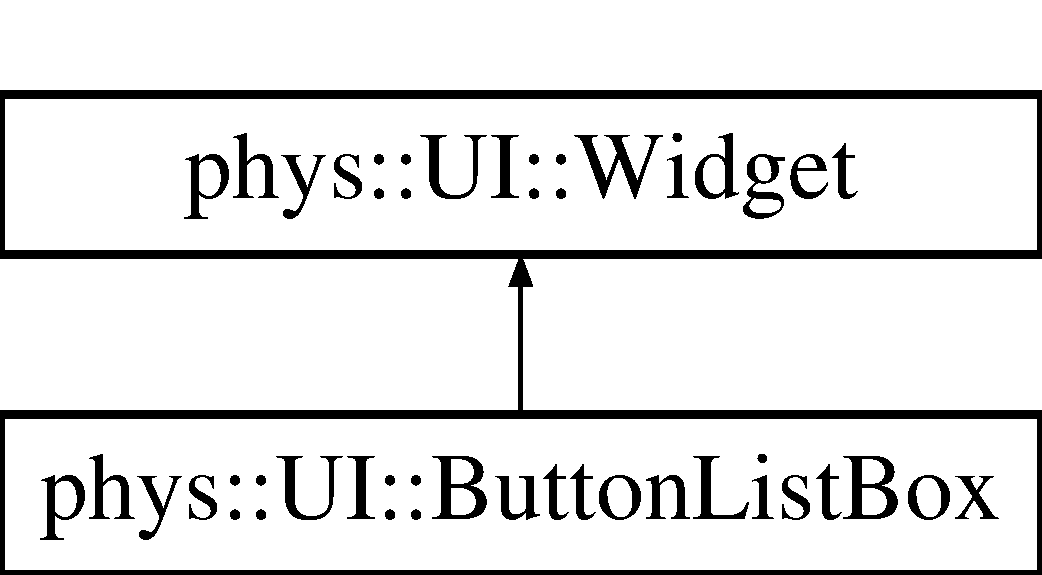
\includegraphics[height=2.000000cm]{classphys_1_1UI_1_1ButtonListBox}
\end{center}
\end{figure}
\subsubsection*{Public Member Functions}
\begin{DoxyCompactItemize}
\item 
virtual \hyperlink{classphys_1_1UI_1_1Button}{Button} $\ast$ \hyperlink{classphys_1_1UI_1_1ButtonListBox_afc976097cd2b1a039882e07272f9a464}{AddSelection} (\hyperlink{namespacephys_a5ce5049f8b4bf88d6413c47b504ebb31}{ConstString} \&name, \hyperlink{namespacephys_a5ce5049f8b4bf88d6413c47b504ebb31}{ConstString} \&BackgroundSprite=\char`\"{}\char`\"{}, \hyperlink{namespacephys_a5ce5049f8b4bf88d6413c47b504ebb31}{ConstString} \&TextLabel=\char`\"{}\char`\"{})
\begin{DoxyCompactList}\small\item\em Adds a selectable button to the list to be displayed. \item\end{DoxyCompactList}\item 
\hyperlink{classphys_1_1UI_1_1ButtonListBox_a43ac98232280969a8ce2641d36658808}{ButtonListBox} (\hyperlink{namespacephys_a5ce5049f8b4bf88d6413c47b504ebb31}{ConstString} \&name, const \hyperlink{structphys_1_1UI_1_1RenderableRect}{RenderableRect} \&Rect, const \hyperlink{namespacephys_af7eb897198d265b8e868f45240230d5f}{Real} \&ScrollbarWidth, const UI::ScrollbarStyle \&ScrollStyle, \hyperlink{classphys_1_1UI_1_1Layer}{Layer} $\ast$PLayer)
\begin{DoxyCompactList}\small\item\em Standard initialization constructor. \item\end{DoxyCompactList}\item 
virtual bool \hyperlink{classphys_1_1UI_1_1ButtonListBox_aaa8b11b174a0475cadee3d3349ef1a58}{CheckMouseHover} ()
\begin{DoxyCompactList}\small\item\em Checks to see if the current mouse position is over this \hyperlink{classphys_1_1UI_1_1Button}{Button} List Box. \item\end{DoxyCompactList}\item 
virtual void \hyperlink{classphys_1_1UI_1_1ButtonListBox_a4ac91d2219d9fa471976bd482dc909b4}{DestroySelection} (\hyperlink{classphys_1_1UI_1_1Button}{Button} $\ast$ToBeDestroyed)
\begin{DoxyCompactList}\small\item\em Destroys a selectable button. \item\end{DoxyCompactList}\item 
virtual void \hyperlink{classphys_1_1UI_1_1ButtonListBox_a2717ab6e1ad39bb7db634a97c4f4157a}{DestroySelection} (\hyperlink{namespacephys_aa03900411993de7fbfec4789bc1d392e}{String} \&ToBeDestroyed)
\begin{DoxyCompactList}\small\item\em Destroys a selectable button. \item\end{DoxyCompactList}\item 
\hypertarget{classphys_1_1UI_1_1ButtonListBox_ae7ea19d82a4c9a7d4262bf41e4204fce}{
virtual void \hyperlink{classphys_1_1UI_1_1ButtonListBox_ae7ea19d82a4c9a7d4262bf41e4204fce}{DisableBorderSelector} ()}
\label{classphys_1_1UI_1_1ButtonListBox_ae7ea19d82a4c9a7d4262bf41e4204fce}

\begin{DoxyCompactList}\small\item\em Disables borders on currently selected buttons if one was enabled. \item\end{DoxyCompactList}\item 
virtual void \hyperlink{classphys_1_1UI_1_1ButtonListBox_a7171571edf9dbf1a5f5543ecdaf119eb}{EnableBorderSelector} (const \hyperlink{namespacephys_af7eb897198d265b8e868f45240230d5f}{Real} \&Width, const \hyperlink{classphys_1_1ColourValue}{ColourValue} \&Colour)
\begin{DoxyCompactList}\small\item\em Enables the setting of a border on the button you select. \item\end{DoxyCompactList}\item 
virtual \hyperlink{classphys_1_1Vector2}{Vector2} \hyperlink{classphys_1_1UI_1_1ButtonListBox_addc5d7c6ab2a48ffa0d4b2e46c20d9a5}{GetActualPosition} ()
\begin{DoxyCompactList}\small\item\em Sets the pixel position of this \hyperlink{classphys_1_1UI_1_1Button}{Button} List Box. \item\end{DoxyCompactList}\item 
virtual \hyperlink{classphys_1_1Vector2}{Vector2} \hyperlink{classphys_1_1UI_1_1ButtonListBox_a77d992f8858bf9b9eeb190dd1ea8a4fd}{GetActualSize} ()
\begin{DoxyCompactList}\small\item\em Sets the pixel size of this \hyperlink{classphys_1_1UI_1_1Button}{Button} List Box. \item\end{DoxyCompactList}\item 
virtual \hyperlink{classphys_1_1UI_1_1Rectangle}{Rectangle} $\ast$ \hyperlink{classphys_1_1UI_1_1ButtonListBox_a043ce9d76af4538043551bf508811b12}{GetBoxBack} ()
\begin{DoxyCompactList}\small\item\em Gets the background of this \hyperlink{classphys_1_1UI_1_1Button}{Button} List Box. \item\end{DoxyCompactList}\item 
virtual \hyperlink{classphys_1_1Vector2}{Vector2} \hyperlink{classphys_1_1UI_1_1ButtonListBox_ab7834542f8940adba8df6b1eace92e95}{GetPosition} ()
\begin{DoxyCompactList}\small\item\em Gets the relative position of this \hyperlink{classphys_1_1UI_1_1Button}{Button} List Box. \item\end{DoxyCompactList}\item 
virtual \hyperlink{classphys_1_1UI_1_1Button}{Button} $\ast$ \hyperlink{classphys_1_1UI_1_1ButtonListBox_a2774799b087576f9085c0d713c129e76}{GetSelected} ()
\begin{DoxyCompactList}\small\item\em Gets the currently selected button. \item\end{DoxyCompactList}\item 
virtual \hyperlink{classphys_1_1UI_1_1Button}{Button} $\ast$ \hyperlink{classphys_1_1UI_1_1ButtonListBox_a88796d75b2677b0a8e5d70fcf3677348}{GetSelection} (\hyperlink{namespacephys_a5ce5049f8b4bf88d6413c47b504ebb31}{ConstString} \&Name)
\begin{DoxyCompactList}\small\item\em Gets a button by name. \item\end{DoxyCompactList}\item 
virtual \hyperlink{classphys_1_1Vector2}{Vector2} \hyperlink{classphys_1_1UI_1_1ButtonListBox_a0084510b0b9c53761e5b4a45f65604ab}{GetSize} ()
\begin{DoxyCompactList}\small\item\em Gets the relative size of this \hyperlink{classphys_1_1UI_1_1Button}{Button} List Box. \item\end{DoxyCompactList}\item 
virtual \hyperlink{classphys_1_1UI_1_1Scrollbar}{UI::Scrollbar} $\ast$ \hyperlink{classphys_1_1UI_1_1ButtonListBox_ad0988e4abe0daef3b9949e42c6dfc5fd}{GetVertScroll} ()
\begin{DoxyCompactList}\small\item\em Gets the scrollbar used within this \hyperlink{classphys_1_1UI_1_1Button}{Button} List Box. \item\end{DoxyCompactList}\item 
\hypertarget{classphys_1_1UI_1_1ButtonListBox_a679eaa7b269f5fa20db2c1bff6bc2d3b}{
virtual void \hyperlink{classphys_1_1UI_1_1ButtonListBox_a679eaa7b269f5fa20db2c1bff6bc2d3b}{Hide} ()}
\label{classphys_1_1UI_1_1ButtonListBox_a679eaa7b269f5fa20db2c1bff6bc2d3b}

\begin{DoxyCompactList}\small\item\em Forces this \hyperlink{classphys_1_1UI_1_1Button}{Button} List Box to hide. \item\end{DoxyCompactList}\item 
virtual bool \hyperlink{classphys_1_1UI_1_1ButtonListBox_a1282a1494079e47b48c8e3296b1a8bb0}{IsVisible} ()
\begin{DoxyCompactList}\small\item\em Gets the visibility of this \hyperlink{classphys_1_1UI_1_1Button}{Button} List Box. \item\end{DoxyCompactList}\item 
virtual void \hyperlink{classphys_1_1UI_1_1ButtonListBox_a3b027750d7d1a5b84a98fc348dee4e64}{SetActualPosition} (const \hyperlink{classphys_1_1Vector2}{Vector2} \&Position)
\begin{DoxyCompactList}\small\item\em Sets the pixel position of this \hyperlink{classphys_1_1UI_1_1Button}{Button} List Box. \item\end{DoxyCompactList}\item 
virtual void \hyperlink{classphys_1_1UI_1_1ButtonListBox_a40f357673d774cbecae7104a02be365e}{SetActualSize} (const \hyperlink{classphys_1_1Vector2}{Vector2} \&Size)
\begin{DoxyCompactList}\small\item\em Sets the pixel size of this \hyperlink{classphys_1_1UI_1_1Button}{Button} List Box. \item\end{DoxyCompactList}\item 
virtual void \hyperlink{classphys_1_1UI_1_1ButtonListBox_ab5caa7d6bd929875bb8ca1278743ff40}{SetAutoHideScroll} (bool AutoHide)
\begin{DoxyCompactList}\small\item\em Eanbles or disables the scrollbar autohide. \item\end{DoxyCompactList}\item 
virtual void \hyperlink{classphys_1_1UI_1_1ButtonListBox_a9c6b0bc4eb93b53c4f7172ce3a537178}{SetPosition} (const \hyperlink{classphys_1_1Vector2}{Vector2} \&Position)
\begin{DoxyCompactList}\small\item\em Sets the relative position of this \hyperlink{classphys_1_1UI_1_1Button}{Button} List Box. \item\end{DoxyCompactList}\item 
virtual void \hyperlink{classphys_1_1UI_1_1ButtonListBox_a843a4975bb7913bcc53d3a66c7f802fa}{SetSelectionDistance} (const \hyperlink{namespacephys_af7eb897198d265b8e868f45240230d5f}{Real} \&Dist)
\begin{DoxyCompactList}\small\item\em Sets the distance apart(and from the sides of box) the Selections will be from each other. \item\end{DoxyCompactList}\item 
virtual void \hyperlink{classphys_1_1UI_1_1ButtonListBox_affc95f7b3c3753b5a89eda7f84c78fb0}{SetSize} (const \hyperlink{classphys_1_1Vector2}{Vector2} \&Size)
\begin{DoxyCompactList}\small\item\em Sets the relative size of this \hyperlink{classphys_1_1UI_1_1Button}{Button} List Box. \item\end{DoxyCompactList}\item 
virtual void \hyperlink{classphys_1_1UI_1_1ButtonListBox_ac14c18e280d1e9fd39a850a9397633e0}{SetTemplateParameters} (\hyperlink{classphys_1_1Vector2}{Vector2} Size, const \hyperlink{namespacephys_a460f6bc24c8dd347b05e0366ae34f34a}{Whole} Glyph)
\begin{DoxyCompactList}\small\item\em Sets the desired size and glyph set provided to all buttons created within this widget. \item\end{DoxyCompactList}\item 
virtual void \hyperlink{classphys_1_1UI_1_1ButtonListBox_acee378e954050801fa8fffe835441bf4}{SetVisible} (bool visible)
\begin{DoxyCompactList}\small\item\em Sets the visibility of this \hyperlink{classphys_1_1UI_1_1Button}{Button} List Box. \item\end{DoxyCompactList}\item 
\hypertarget{classphys_1_1UI_1_1ButtonListBox_ad41d563b4fab1699fb14b56f776d5b1f}{
virtual void \hyperlink{classphys_1_1UI_1_1ButtonListBox_ad41d563b4fab1699fb14b56f776d5b1f}{Show} ()}
\label{classphys_1_1UI_1_1ButtonListBox_ad41d563b4fab1699fb14b56f776d5b1f}

\begin{DoxyCompactList}\small\item\em Forces this \hyperlink{classphys_1_1UI_1_1Button}{Button} List Box to be shown. \item\end{DoxyCompactList}\item 
\hypertarget{classphys_1_1UI_1_1ButtonListBox_afb7cf0d76f1f6825276694f0ebb7f4a6}{
virtual \hyperlink{classphys_1_1UI_1_1ButtonListBox_afb7cf0d76f1f6825276694f0ebb7f4a6}{$\sim$ButtonListBox} ()}
\label{classphys_1_1UI_1_1ButtonListBox_afb7cf0d76f1f6825276694f0ebb7f4a6}

\begin{DoxyCompactList}\small\item\em Standard destructor. \item\end{DoxyCompactList}\end{DoxyCompactItemize}
\subsubsection*{Protected Member Functions}
\begin{DoxyCompactItemize}
\item 
\hypertarget{classphys_1_1UI_1_1ButtonListBox_a1b8d7f3de8e241c940f022ea5b5e1c97}{
virtual void \hyperlink{classphys_1_1UI_1_1ButtonListBox_a1b8d7f3de8e241c940f022ea5b5e1c97}{CalculateVisibleSelections} ()}
\label{classphys_1_1UI_1_1ButtonListBox_a1b8d7f3de8e241c940f022ea5b5e1c97}

\begin{DoxyCompactList}\small\item\em Determines how many items can be displayed in the box at once. \item\end{DoxyCompactList}\item 
\hypertarget{classphys_1_1UI_1_1ButtonListBox_a6fbb3046819a0dace3a178a752efe652}{
virtual void \hyperlink{classphys_1_1UI_1_1ButtonListBox_a6fbb3046819a0dace3a178a752efe652}{DrawList} ()}
\label{classphys_1_1UI_1_1ButtonListBox_a6fbb3046819a0dace3a178a752efe652}

\begin{DoxyCompactList}\small\item\em Updates the list of Visible buttons and hides the rest. \item\end{DoxyCompactList}\item 
\hypertarget{classphys_1_1UI_1_1ButtonListBox_a4c412be3030aea2e3ca2ce946a4cdd26}{
virtual void \hyperlink{classphys_1_1UI_1_1ButtonListBox_a4c412be3030aea2e3ca2ce946a4cdd26}{Update} (bool Force=false)}
\label{classphys_1_1UI_1_1ButtonListBox_a4c412be3030aea2e3ca2ce946a4cdd26}

\begin{DoxyCompactList}\small\item\em For use with widget update/automation. \item\end{DoxyCompactList}\end{DoxyCompactItemize}
\subsubsection*{Protected Attributes}
\begin{DoxyCompactItemize}
\item 
\hypertarget{classphys_1_1UI_1_1ButtonListBox_ad32c9f2edc747abc532ff079e4cb9dc5}{
bool {\bfseries AutoHideScroll}}
\label{classphys_1_1UI_1_1ButtonListBox_ad32c9f2edc747abc532ff079e4cb9dc5}

\item 
\hypertarget{classphys_1_1UI_1_1ButtonListBox_abea496f1f59230f00ea03af54264804b}{
\hyperlink{classphys_1_1ColourValue}{ColourValue} {\bfseries BorderColour}}
\label{classphys_1_1UI_1_1ButtonListBox_abea496f1f59230f00ea03af54264804b}

\item 
\hypertarget{classphys_1_1UI_1_1ButtonListBox_a84d6d689a273e77252f248c81bd1d670}{
\hyperlink{namespacephys_af7eb897198d265b8e868f45240230d5f}{Real} {\bfseries BorderWidth}}
\label{classphys_1_1UI_1_1ButtonListBox_a84d6d689a273e77252f248c81bd1d670}

\item 
\hypertarget{classphys_1_1UI_1_1ButtonListBox_a49b55881aff0481c77646cc673cd5b16}{
\hyperlink{classphys_1_1UI_1_1Rectangle}{Rectangle} $\ast$ {\bfseries BoxBack}}
\label{classphys_1_1UI_1_1ButtonListBox_a49b55881aff0481c77646cc673cd5b16}

\item 
\hypertarget{classphys_1_1UI_1_1ButtonListBox_a1c3b09eca31eb3dff7dfab82624b0e45}{
\hyperlink{namespacephys_af7eb897198d265b8e868f45240230d5f}{Real} {\bfseries LastScrollValue}}
\label{classphys_1_1UI_1_1ButtonListBox_a1c3b09eca31eb3dff7dfab82624b0e45}

\item 
\hypertarget{classphys_1_1UI_1_1ButtonListBox_a9414e2009038dcd9dbb31464f63b563a}{
\hyperlink{namespacephys_a460f6bc24c8dd347b05e0366ae34f34a}{Whole} {\bfseries NumVisible}}
\label{classphys_1_1UI_1_1ButtonListBox_a9414e2009038dcd9dbb31464f63b563a}

\item 
\hypertarget{classphys_1_1UI_1_1ButtonListBox_ae12fd29fa8ece99377bf782eed261bb9}{
\hyperlink{classphys_1_1UI_1_1Button}{Button} $\ast$ {\bfseries Selected}}
\label{classphys_1_1UI_1_1ButtonListBox_ae12fd29fa8ece99377bf782eed261bb9}

\item 
\hypertarget{classphys_1_1UI_1_1ButtonListBox_ab26148ae8dec6c70c8c812f61cbc29f5}{
\hyperlink{namespacephys_af7eb897198d265b8e868f45240230d5f}{Real} {\bfseries SelectionDist}}
\label{classphys_1_1UI_1_1ButtonListBox_ab26148ae8dec6c70c8c812f61cbc29f5}

\item 
\hypertarget{classphys_1_1UI_1_1ButtonListBox_a1f68770e3eb20daefeefb34fb0f7ad5c}{
std::vector$<$ \hyperlink{classphys_1_1UI_1_1Button}{Button} $\ast$ $>$ {\bfseries Selections}}
\label{classphys_1_1UI_1_1ButtonListBox_a1f68770e3eb20daefeefb34fb0f7ad5c}

\item 
\hypertarget{classphys_1_1UI_1_1ButtonListBox_a4284fcee343ce2bbb178d560a5712e6b}{
\hyperlink{namespacephys_a460f6bc24c8dd347b05e0366ae34f34a}{Whole} {\bfseries TGlyph}}
\label{classphys_1_1UI_1_1ButtonListBox_a4284fcee343ce2bbb178d560a5712e6b}

\item 
\hypertarget{classphys_1_1UI_1_1ButtonListBox_a3b2483012699ef522c592ecefb30a82a}{
\hyperlink{classphys_1_1Vector2}{Vector2} {\bfseries TSize}}
\label{classphys_1_1UI_1_1ButtonListBox_a3b2483012699ef522c592ecefb30a82a}

\item 
\hyperlink{classphys_1_1UI_1_1Scrollbar}{UI::Scrollbar} $\ast$ \hyperlink{classphys_1_1UI_1_1ButtonListBox_aa47d94d75c58e3408a97766eace2c20e}{VertScroll}
\item 
\hypertarget{classphys_1_1UI_1_1ButtonListBox_aee57382752a939219a1bcdc67229dadf}{
std::vector$<$ \hyperlink{classphys_1_1UI_1_1Button}{Button} $\ast$ $>$ {\bfseries VisibleSelections}}
\label{classphys_1_1UI_1_1ButtonListBox_aee57382752a939219a1bcdc67229dadf}

\end{DoxyCompactItemize}


\subsubsection{Detailed Description}
This is a widget for displaying a list of buttons in a box. 

Definition at line 60 of file uibuttonlistbox.h.



\subsubsection{Constructor \& Destructor Documentation}
\hypertarget{classphys_1_1UI_1_1ButtonListBox_a43ac98232280969a8ce2641d36658808}{
\index{phys::UI::ButtonListBox@{phys::UI::ButtonListBox}!ButtonListBox@{ButtonListBox}}
\index{ButtonListBox@{ButtonListBox}!phys::UI::ButtonListBox@{phys::UI::ButtonListBox}}
\paragraph[{ButtonListBox}]{\setlength{\rightskip}{0pt plus 5cm}phys::UI::ButtonListBox::ButtonListBox (
\begin{DoxyParamCaption}
\item[{{\bf ConstString} \&}]{name, }
\item[{const {\bf RenderableRect} \&}]{Rect, }
\item[{const {\bf Real} \&}]{ScrollbarWidth, }
\item[{const UI::ScrollbarStyle \&}]{ScrollStyle, }
\item[{{\bf Layer} $\ast$}]{PLayer}
\end{DoxyParamCaption}
)}\hfill}
\label{classphys_1_1UI_1_1ButtonListBox_a43ac98232280969a8ce2641d36658808}


Standard initialization constructor. 


\begin{DoxyParams}{Parameters}
{\em name} & The name of the \hyperlink{classphys_1_1UI_1_1Button}{Button} List Box. \\
\hline
{\em Rect} & The Rect representing the position and size of the \hyperlink{classphys_1_1UI_1_1Button}{Button} List Box. \\
\hline
{\em ScrollbarWidth} & The width of the vertical scrollbar. If the Rect passed in is relative, this will expect Scrollwidth to be relative as well. If a horizontal scrollbar is needed it'll use the equal value in pixels(to avoid the stretched look. \\
\hline
{\em ScrollStyle} & The style of the scrollbar you want for this \hyperlink{classphys_1_1UI_1_1Button}{Button} List Box. See \hyperlink{classphys_1_1UI_1_1Scrollbar}{Scrollbar} class for more information. \\
\hline
{\em \hyperlink{classphys_1_1UI_1_1Layer}{Layer}} & The parent layer this \hyperlink{classphys_1_1UI_1_1Button}{Button} List Box belongs to. \\
\hline
\end{DoxyParams}


\begin{Desc}
\item[\hyperlink{todo__todo000024}{Todo}]Fourth instance of needing to include the namespace in the declaration seemingly needlessly. \end{Desc}




Definition at line 61 of file uibuttonlistbox.cpp.



\subsubsection{Member Function Documentation}
\hypertarget{classphys_1_1UI_1_1ButtonListBox_afc976097cd2b1a039882e07272f9a464}{
\index{phys::UI::ButtonListBox@{phys::UI::ButtonListBox}!AddSelection@{AddSelection}}
\index{AddSelection@{AddSelection}!phys::UI::ButtonListBox@{phys::UI::ButtonListBox}}
\paragraph[{AddSelection}]{\setlength{\rightskip}{0pt plus 5cm}{\bf Button} $\ast$ phys::UI::ButtonListBox::AddSelection (
\begin{DoxyParamCaption}
\item[{{\bf ConstString} \&}]{name, }
\item[{{\bf ConstString} \&}]{BackgroundSprite = {\ttfamily \char`\"{}\char`\"{}}, }
\item[{{\bf ConstString} \&}]{TextLabel = {\ttfamily \char`\"{}\char`\"{}}}
\end{DoxyParamCaption}
)\hspace{0.3cm}{\ttfamily  \mbox{[}virtual\mbox{]}}}\hfill}
\label{classphys_1_1UI_1_1ButtonListBox_afc976097cd2b1a039882e07272f9a464}


Adds a selectable button to the list to be displayed. 


\begin{DoxyParams}{Parameters}
{\em BackgroundSprite} & Optional, name of the sprite to set as it's background. Ignored if the string is empty. \\
\hline
{\em TextLabel} & Optional, will create a text button instead of a regular button and set it's text. Ignored if the string is empty. \par
 \par
 Note: If a Text button is created, you can't revert it to a regular button and vice versa. You'll have to destroy the selection and make a new one. In the case of having a text button, you can however still set it's text to an empty string. \\
\hline
\end{DoxyParams}
\begin{DoxyReturn}{Returns}
Returns a pointer to the created button. 
\end{DoxyReturn}


Definition at line 302 of file uibuttonlistbox.cpp.

\hypertarget{classphys_1_1UI_1_1ButtonListBox_aaa8b11b174a0475cadee3d3349ef1a58}{
\index{phys::UI::ButtonListBox@{phys::UI::ButtonListBox}!CheckMouseHover@{CheckMouseHover}}
\index{CheckMouseHover@{CheckMouseHover}!phys::UI::ButtonListBox@{phys::UI::ButtonListBox}}
\paragraph[{CheckMouseHover}]{\setlength{\rightskip}{0pt plus 5cm}bool phys::UI::ButtonListBox::CheckMouseHover (
\begin{DoxyParamCaption}
{}
\end{DoxyParamCaption}
)\hspace{0.3cm}{\ttfamily  \mbox{[}virtual\mbox{]}}}\hfill}
\label{classphys_1_1UI_1_1ButtonListBox_aaa8b11b174a0475cadee3d3349ef1a58}


Checks to see if the current mouse position is over this \hyperlink{classphys_1_1UI_1_1Button}{Button} List Box. 

\begin{DoxyReturn}{Returns}
Returns a bool value, true if the mouse is over this \hyperlink{classphys_1_1UI_1_1Button}{Button} List Box, false if it's not. 
\end{DoxyReturn}


Implements \hyperlink{classphys_1_1UI_1_1Widget_a613df6dbb42efe139d185043a00259dc}{phys::UI::Widget}.



Definition at line 262 of file uibuttonlistbox.cpp.

\hypertarget{classphys_1_1UI_1_1ButtonListBox_a4ac91d2219d9fa471976bd482dc909b4}{
\index{phys::UI::ButtonListBox@{phys::UI::ButtonListBox}!DestroySelection@{DestroySelection}}
\index{DestroySelection@{DestroySelection}!phys::UI::ButtonListBox@{phys::UI::ButtonListBox}}
\paragraph[{DestroySelection}]{\setlength{\rightskip}{0pt plus 5cm}void phys::UI::ButtonListBox::DestroySelection (
\begin{DoxyParamCaption}
\item[{{\bf Button} $\ast$}]{ToBeDestroyed}
\end{DoxyParamCaption}
)\hspace{0.3cm}{\ttfamily  \mbox{[}virtual\mbox{]}}}\hfill}
\label{classphys_1_1UI_1_1ButtonListBox_a4ac91d2219d9fa471976bd482dc909b4}


Destroys a selectable button. 


\begin{DoxyParams}{Parameters}
{\em ToBeDestroyed} & A pointer to the button you want destroyed and removed from this list. \\
\hline
\end{DoxyParams}


Definition at line 337 of file uibuttonlistbox.cpp.

\hypertarget{classphys_1_1UI_1_1ButtonListBox_a2717ab6e1ad39bb7db634a97c4f4157a}{
\index{phys::UI::ButtonListBox@{phys::UI::ButtonListBox}!DestroySelection@{DestroySelection}}
\index{DestroySelection@{DestroySelection}!phys::UI::ButtonListBox@{phys::UI::ButtonListBox}}
\paragraph[{DestroySelection}]{\setlength{\rightskip}{0pt plus 5cm}void phys::UI::ButtonListBox::DestroySelection (
\begin{DoxyParamCaption}
\item[{{\bf String} \&}]{ToBeDestroyed}
\end{DoxyParamCaption}
)\hspace{0.3cm}{\ttfamily  \mbox{[}virtual\mbox{]}}}\hfill}
\label{classphys_1_1UI_1_1ButtonListBox_a2717ab6e1ad39bb7db634a97c4f4157a}


Destroys a selectable button. 


\begin{DoxyParams}{Parameters}
{\em ToBeDestroyed} & A string naming the button you want destroyed and removed from this list. \\
\hline
\end{DoxyParams}


Definition at line 351 of file uibuttonlistbox.cpp.

\hypertarget{classphys_1_1UI_1_1ButtonListBox_a7171571edf9dbf1a5f5543ecdaf119eb}{
\index{phys::UI::ButtonListBox@{phys::UI::ButtonListBox}!EnableBorderSelector@{EnableBorderSelector}}
\index{EnableBorderSelector@{EnableBorderSelector}!phys::UI::ButtonListBox@{phys::UI::ButtonListBox}}
\paragraph[{EnableBorderSelector}]{\setlength{\rightskip}{0pt plus 5cm}void phys::UI::ButtonListBox::EnableBorderSelector (
\begin{DoxyParamCaption}
\item[{const {\bf Real} \&}]{Width, }
\item[{const {\bf ColourValue} \&}]{Colour}
\end{DoxyParamCaption}
)\hspace{0.3cm}{\ttfamily  \mbox{[}virtual\mbox{]}}}\hfill}
\label{classphys_1_1UI_1_1ButtonListBox_a7171571edf9dbf1a5f5543ecdaf119eb}


Enables the setting of a border on the button you select. 


\begin{DoxyParams}{Parameters}
{\em Width} & The width of the border in pixels. \\
\hline
{\em Colour} & The colour of the border. \\
\hline
\end{DoxyParams}


Definition at line 377 of file uibuttonlistbox.cpp.

\hypertarget{classphys_1_1UI_1_1ButtonListBox_addc5d7c6ab2a48ffa0d4b2e46c20d9a5}{
\index{phys::UI::ButtonListBox@{phys::UI::ButtonListBox}!GetActualPosition@{GetActualPosition}}
\index{GetActualPosition@{GetActualPosition}!phys::UI::ButtonListBox@{phys::UI::ButtonListBox}}
\paragraph[{GetActualPosition}]{\setlength{\rightskip}{0pt plus 5cm}{\bf Vector2} phys::UI::ButtonListBox::GetActualPosition (
\begin{DoxyParamCaption}
{}
\end{DoxyParamCaption}
)\hspace{0.3cm}{\ttfamily  \mbox{[}virtual\mbox{]}}}\hfill}
\label{classphys_1_1UI_1_1ButtonListBox_addc5d7c6ab2a48ffa0d4b2e46c20d9a5}


Sets the pixel position of this \hyperlink{classphys_1_1UI_1_1Button}{Button} List Box. 

\begin{DoxyReturn}{Returns}
Returns a vector2 representing the pixel position of this \hyperlink{classphys_1_1UI_1_1Button}{Button} List Box. 
\end{DoxyReturn}


Implements \hyperlink{classphys_1_1UI_1_1Widget_a0a29fecff7f56d7909f65fd63b0990e7}{phys::UI::Widget}.



Definition at line 412 of file uibuttonlistbox.cpp.

\hypertarget{classphys_1_1UI_1_1ButtonListBox_a77d992f8858bf9b9eeb190dd1ea8a4fd}{
\index{phys::UI::ButtonListBox@{phys::UI::ButtonListBox}!GetActualSize@{GetActualSize}}
\index{GetActualSize@{GetActualSize}!phys::UI::ButtonListBox@{phys::UI::ButtonListBox}}
\paragraph[{GetActualSize}]{\setlength{\rightskip}{0pt plus 5cm}{\bf Vector2} phys::UI::ButtonListBox::GetActualSize (
\begin{DoxyParamCaption}
{}
\end{DoxyParamCaption}
)\hspace{0.3cm}{\ttfamily  \mbox{[}virtual\mbox{]}}}\hfill}
\label{classphys_1_1UI_1_1ButtonListBox_a77d992f8858bf9b9eeb190dd1ea8a4fd}


Sets the pixel size of this \hyperlink{classphys_1_1UI_1_1Button}{Button} List Box. 

\begin{DoxyReturn}{Returns}
Returns a vector2 representing the pixel size of this \hyperlink{classphys_1_1UI_1_1Button}{Button} List Box. 
\end{DoxyReturn}


Implements \hyperlink{classphys_1_1UI_1_1Widget_af3a685621ed220748c0940ea38c96ed2}{phys::UI::Widget}.



Definition at line 446 of file uibuttonlistbox.cpp.

\hypertarget{classphys_1_1UI_1_1ButtonListBox_a043ce9d76af4538043551bf508811b12}{
\index{phys::UI::ButtonListBox@{phys::UI::ButtonListBox}!GetBoxBack@{GetBoxBack}}
\index{GetBoxBack@{GetBoxBack}!phys::UI::ButtonListBox@{phys::UI::ButtonListBox}}
\paragraph[{GetBoxBack}]{\setlength{\rightskip}{0pt plus 5cm}{\bf Rectangle} $\ast$ phys::UI::ButtonListBox::GetBoxBack (
\begin{DoxyParamCaption}
{}
\end{DoxyParamCaption}
)\hspace{0.3cm}{\ttfamily  \mbox{[}virtual\mbox{]}}}\hfill}
\label{classphys_1_1UI_1_1ButtonListBox_a043ce9d76af4538043551bf508811b12}


Gets the background of this \hyperlink{classphys_1_1UI_1_1Button}{Button} List Box. 

\begin{DoxyReturn}{Returns}
Returns a pointer to the background of this \hyperlink{classphys_1_1UI_1_1Button}{Button} List Box. 
\end{DoxyReturn}


Definition at line 456 of file uibuttonlistbox.cpp.

\hypertarget{classphys_1_1UI_1_1ButtonListBox_ab7834542f8940adba8df6b1eace92e95}{
\index{phys::UI::ButtonListBox@{phys::UI::ButtonListBox}!GetPosition@{GetPosition}}
\index{GetPosition@{GetPosition}!phys::UI::ButtonListBox@{phys::UI::ButtonListBox}}
\paragraph[{GetPosition}]{\setlength{\rightskip}{0pt plus 5cm}{\bf Vector2} phys::UI::ButtonListBox::GetPosition (
\begin{DoxyParamCaption}
{}
\end{DoxyParamCaption}
)\hspace{0.3cm}{\ttfamily  \mbox{[}virtual\mbox{]}}}\hfill}
\label{classphys_1_1UI_1_1ButtonListBox_ab7834542f8940adba8df6b1eace92e95}


Gets the relative position of this \hyperlink{classphys_1_1UI_1_1Button}{Button} List Box. 

The position is relative to the screen size. Values range from 0.0 to 1.0. \begin{DoxyReturn}{Returns}
Returns a vector2 representing the relative position of this \hyperlink{classphys_1_1UI_1_1Button}{Button} List Box. 
\end{DoxyReturn}


Implements \hyperlink{classphys_1_1UI_1_1Widget_a3e464b028b0d1b5755923b8790260c33}{phys::UI::Widget}.



Definition at line 398 of file uibuttonlistbox.cpp.

\hypertarget{classphys_1_1UI_1_1ButtonListBox_a2774799b087576f9085c0d713c129e76}{
\index{phys::UI::ButtonListBox@{phys::UI::ButtonListBox}!GetSelected@{GetSelected}}
\index{GetSelected@{GetSelected}!phys::UI::ButtonListBox@{phys::UI::ButtonListBox}}
\paragraph[{GetSelected}]{\setlength{\rightskip}{0pt plus 5cm}{\bf Button} $\ast$ phys::UI::ButtonListBox::GetSelected (
\begin{DoxyParamCaption}
{}
\end{DoxyParamCaption}
)\hspace{0.3cm}{\ttfamily  \mbox{[}virtual\mbox{]}}}\hfill}
\label{classphys_1_1UI_1_1ButtonListBox_a2774799b087576f9085c0d713c129e76}


Gets the currently selected button. 

\begin{DoxyReturn}{Returns}
Returns a pointer to the currently selected button, or NULL if none are selected. 
\end{DoxyReturn}


Definition at line 451 of file uibuttonlistbox.cpp.

\hypertarget{classphys_1_1UI_1_1ButtonListBox_a88796d75b2677b0a8e5d70fcf3677348}{
\index{phys::UI::ButtonListBox@{phys::UI::ButtonListBox}!GetSelection@{GetSelection}}
\index{GetSelection@{GetSelection}!phys::UI::ButtonListBox@{phys::UI::ButtonListBox}}
\paragraph[{GetSelection}]{\setlength{\rightskip}{0pt plus 5cm}{\bf Button} $\ast$ phys::UI::ButtonListBox::GetSelection (
\begin{DoxyParamCaption}
\item[{{\bf ConstString} \&}]{Name}
\end{DoxyParamCaption}
)\hspace{0.3cm}{\ttfamily  \mbox{[}virtual\mbox{]}}}\hfill}
\label{classphys_1_1UI_1_1ButtonListBox_a88796d75b2677b0a8e5d70fcf3677348}


Gets a button by name. 


\begin{DoxyParams}{Parameters}
{\em Name} & The name of the selectable button you want to get. \\
\hline
\end{DoxyParams}
\begin{DoxyReturn}{Returns}
Returns a pointer to the named button. 
\end{DoxyReturn}


Definition at line 324 of file uibuttonlistbox.cpp.

\hypertarget{classphys_1_1UI_1_1ButtonListBox_a0084510b0b9c53761e5b4a45f65604ab}{
\index{phys::UI::ButtonListBox@{phys::UI::ButtonListBox}!GetSize@{GetSize}}
\index{GetSize@{GetSize}!phys::UI::ButtonListBox@{phys::UI::ButtonListBox}}
\paragraph[{GetSize}]{\setlength{\rightskip}{0pt plus 5cm}{\bf Vector2} phys::UI::ButtonListBox::GetSize (
\begin{DoxyParamCaption}
{}
\end{DoxyParamCaption}
)\hspace{0.3cm}{\ttfamily  \mbox{[}virtual\mbox{]}}}\hfill}
\label{classphys_1_1UI_1_1ButtonListBox_a0084510b0b9c53761e5b4a45f65604ab}


Gets the relative size of this \hyperlink{classphys_1_1UI_1_1Button}{Button} List Box. 

The size is relative to the screen size. Values range from 0.0 to 1.0. \begin{DoxyReturn}{Returns}
Returns a vector2 representing the relative size of this \hyperlink{classphys_1_1UI_1_1Button}{Button} List Box. 
\end{DoxyReturn}


Implements \hyperlink{classphys_1_1UI_1_1Widget_a07039c19e57de314147ce066417da0a2}{phys::UI::Widget}.



Definition at line 429 of file uibuttonlistbox.cpp.

\hypertarget{classphys_1_1UI_1_1ButtonListBox_ad0988e4abe0daef3b9949e42c6dfc5fd}{
\index{phys::UI::ButtonListBox@{phys::UI::ButtonListBox}!GetVertScroll@{GetVertScroll}}
\index{GetVertScroll@{GetVertScroll}!phys::UI::ButtonListBox@{phys::UI::ButtonListBox}}
\paragraph[{GetVertScroll}]{\setlength{\rightskip}{0pt plus 5cm}{\bf UI::Scrollbar} $\ast$ phys::UI::ButtonListBox::GetVertScroll (
\begin{DoxyParamCaption}
{}
\end{DoxyParamCaption}
)\hspace{0.3cm}{\ttfamily  \mbox{[}virtual\mbox{]}}}\hfill}
\label{classphys_1_1UI_1_1ButtonListBox_ad0988e4abe0daef3b9949e42c6dfc5fd}


Gets the scrollbar used within this \hyperlink{classphys_1_1UI_1_1Button}{Button} List Box. 

\begin{DoxyReturn}{Returns}
Returns a pointer to the scrollbar of this \hyperlink{classphys_1_1UI_1_1Button}{Button} List Box. 
\end{DoxyReturn}


Definition at line 461 of file uibuttonlistbox.cpp.

\hypertarget{classphys_1_1UI_1_1ButtonListBox_a1282a1494079e47b48c8e3296b1a8bb0}{
\index{phys::UI::ButtonListBox@{phys::UI::ButtonListBox}!IsVisible@{IsVisible}}
\index{IsVisible@{IsVisible}!phys::UI::ButtonListBox@{phys::UI::ButtonListBox}}
\paragraph[{IsVisible}]{\setlength{\rightskip}{0pt plus 5cm}bool phys::UI::ButtonListBox::IsVisible (
\begin{DoxyParamCaption}
{}
\end{DoxyParamCaption}
)\hspace{0.3cm}{\ttfamily  \mbox{[}virtual\mbox{]}}}\hfill}
\label{classphys_1_1UI_1_1ButtonListBox_a1282a1494079e47b48c8e3296b1a8bb0}


Gets the visibility of this \hyperlink{classphys_1_1UI_1_1Button}{Button} List Box. 

\begin{DoxyReturn}{Returns}
Returns a bool representing the visibility of this \hyperlink{classphys_1_1UI_1_1Button}{Button} List Box. 
\end{DoxyReturn}


Implements \hyperlink{classphys_1_1UI_1_1Widget_aaf1a1bd31b8e626467ce9cdb69bdf7ac}{phys::UI::Widget}.



Definition at line 237 of file uibuttonlistbox.cpp.

\hypertarget{classphys_1_1UI_1_1ButtonListBox_a3b027750d7d1a5b84a98fc348dee4e64}{
\index{phys::UI::ButtonListBox@{phys::UI::ButtonListBox}!SetActualPosition@{SetActualPosition}}
\index{SetActualPosition@{SetActualPosition}!phys::UI::ButtonListBox@{phys::UI::ButtonListBox}}
\paragraph[{SetActualPosition}]{\setlength{\rightskip}{0pt plus 5cm}void phys::UI::ButtonListBox::SetActualPosition (
\begin{DoxyParamCaption}
\item[{const {\bf Vector2} \&}]{Position}
\end{DoxyParamCaption}
)\hspace{0.3cm}{\ttfamily  \mbox{[}virtual\mbox{]}}}\hfill}
\label{classphys_1_1UI_1_1ButtonListBox_a3b027750d7d1a5b84a98fc348dee4e64}


Sets the pixel position of this \hyperlink{classphys_1_1UI_1_1Button}{Button} List Box. 


\begin{DoxyParams}{Parameters}
{\em Position} & A vector2 representing the pixel position of this \hyperlink{classphys_1_1UI_1_1Button}{Button} List Box. \\
\hline
\end{DoxyParams}


Implements \hyperlink{classphys_1_1UI_1_1Widget_a77727351d98b10f1f4eb45048cb882e3}{phys::UI::Widget}.



Definition at line 403 of file uibuttonlistbox.cpp.

\hypertarget{classphys_1_1UI_1_1ButtonListBox_a40f357673d774cbecae7104a02be365e}{
\index{phys::UI::ButtonListBox@{phys::UI::ButtonListBox}!SetActualSize@{SetActualSize}}
\index{SetActualSize@{SetActualSize}!phys::UI::ButtonListBox@{phys::UI::ButtonListBox}}
\paragraph[{SetActualSize}]{\setlength{\rightskip}{0pt plus 5cm}void phys::UI::ButtonListBox::SetActualSize (
\begin{DoxyParamCaption}
\item[{const {\bf Vector2} \&}]{Size}
\end{DoxyParamCaption}
)\hspace{0.3cm}{\ttfamily  \mbox{[}virtual\mbox{]}}}\hfill}
\label{classphys_1_1UI_1_1ButtonListBox_a40f357673d774cbecae7104a02be365e}


Sets the pixel size of this \hyperlink{classphys_1_1UI_1_1Button}{Button} List Box. 


\begin{DoxyParams}{Parameters}
{\em Size} & A vector2 representing the pixel size of this \hyperlink{classphys_1_1UI_1_1Button}{Button} List Box. \\
\hline
\end{DoxyParams}


Implements \hyperlink{classphys_1_1UI_1_1Widget_acda63a62fa158d5fe00c86f50e5c120d}{phys::UI::Widget}.



Definition at line 434 of file uibuttonlistbox.cpp.

\hypertarget{classphys_1_1UI_1_1ButtonListBox_ab5caa7d6bd929875bb8ca1278743ff40}{
\index{phys::UI::ButtonListBox@{phys::UI::ButtonListBox}!SetAutoHideScroll@{SetAutoHideScroll}}
\index{SetAutoHideScroll@{SetAutoHideScroll}!phys::UI::ButtonListBox@{phys::UI::ButtonListBox}}
\paragraph[{SetAutoHideScroll}]{\setlength{\rightskip}{0pt plus 5cm}void phys::UI::ButtonListBox::SetAutoHideScroll (
\begin{DoxyParamCaption}
\item[{bool}]{AutoHide}
\end{DoxyParamCaption}
)\hspace{0.3cm}{\ttfamily  \mbox{[}virtual\mbox{]}}}\hfill}
\label{classphys_1_1UI_1_1ButtonListBox_ab5caa7d6bd929875bb8ca1278743ff40}


Eanbles or disables the scrollbar autohide. 


\begin{DoxyParams}{Parameters}
{\em AutoHide} & A bool indicating whether or not to auto hide the scrollbar. \\
\hline
\end{DoxyParams}


Definition at line 370 of file uibuttonlistbox.cpp.

\hypertarget{classphys_1_1UI_1_1ButtonListBox_a9c6b0bc4eb93b53c4f7172ce3a537178}{
\index{phys::UI::ButtonListBox@{phys::UI::ButtonListBox}!SetPosition@{SetPosition}}
\index{SetPosition@{SetPosition}!phys::UI::ButtonListBox@{phys::UI::ButtonListBox}}
\paragraph[{SetPosition}]{\setlength{\rightskip}{0pt plus 5cm}void phys::UI::ButtonListBox::SetPosition (
\begin{DoxyParamCaption}
\item[{const {\bf Vector2} \&}]{Position}
\end{DoxyParamCaption}
)\hspace{0.3cm}{\ttfamily  \mbox{[}virtual\mbox{]}}}\hfill}
\label{classphys_1_1UI_1_1ButtonListBox_a9c6b0bc4eb93b53c4f7172ce3a537178}


Sets the relative position of this \hyperlink{classphys_1_1UI_1_1Button}{Button} List Box. 

The position is relative to the screen size. Values range from 0.0 to 1.0. 
\begin{DoxyParams}{Parameters}
{\em Position} & A vector2 representing the relative position of this \hyperlink{classphys_1_1UI_1_1Button}{Button} List Box. \\
\hline
\end{DoxyParams}


Implements \hyperlink{classphys_1_1UI_1_1Widget_a3ef894be2c0868105b2bf495ae944d00}{phys::UI::Widget}.



Definition at line 389 of file uibuttonlistbox.cpp.

\hypertarget{classphys_1_1UI_1_1ButtonListBox_a843a4975bb7913bcc53d3a66c7f802fa}{
\index{phys::UI::ButtonListBox@{phys::UI::ButtonListBox}!SetSelectionDistance@{SetSelectionDistance}}
\index{SetSelectionDistance@{SetSelectionDistance}!phys::UI::ButtonListBox@{phys::UI::ButtonListBox}}
\paragraph[{SetSelectionDistance}]{\setlength{\rightskip}{0pt plus 5cm}void phys::UI::ButtonListBox::SetSelectionDistance (
\begin{DoxyParamCaption}
\item[{const {\bf Real} \&}]{Dist}
\end{DoxyParamCaption}
)\hspace{0.3cm}{\ttfamily  \mbox{[}virtual\mbox{]}}}\hfill}
\label{classphys_1_1UI_1_1ButtonListBox_a843a4975bb7913bcc53d3a66c7f802fa}


Sets the distance apart(and from the sides of box) the Selections will be from each other. 

This function expects a relative value to the screen size(0.0 to 1.0). This value defaults to 0.025. 
\begin{DoxyParams}{Parameters}
{\em Dist} & A relative value for the distance to be used when determining the positions of Selections. \\
\hline
\end{DoxyParams}


Definition at line 365 of file uibuttonlistbox.cpp.

\hypertarget{classphys_1_1UI_1_1ButtonListBox_affc95f7b3c3753b5a89eda7f84c78fb0}{
\index{phys::UI::ButtonListBox@{phys::UI::ButtonListBox}!SetSize@{SetSize}}
\index{SetSize@{SetSize}!phys::UI::ButtonListBox@{phys::UI::ButtonListBox}}
\paragraph[{SetSize}]{\setlength{\rightskip}{0pt plus 5cm}void phys::UI::ButtonListBox::SetSize (
\begin{DoxyParamCaption}
\item[{const {\bf Vector2} \&}]{Size}
\end{DoxyParamCaption}
)\hspace{0.3cm}{\ttfamily  \mbox{[}virtual\mbox{]}}}\hfill}
\label{classphys_1_1UI_1_1ButtonListBox_affc95f7b3c3753b5a89eda7f84c78fb0}


Sets the relative size of this \hyperlink{classphys_1_1UI_1_1Button}{Button} List Box. 

The size is relative to the screen size. Values range from 0.0 to 1.0. 
\begin{DoxyParams}{Parameters}
{\em Size} & A vector2 representing the relative size of this \hyperlink{classphys_1_1UI_1_1Button}{Button} List Box. \\
\hline
\end{DoxyParams}


Implements \hyperlink{classphys_1_1UI_1_1Widget_a00f73c12583d25a75c089f944075b24d}{phys::UI::Widget}.



Definition at line 417 of file uibuttonlistbox.cpp.

\hypertarget{classphys_1_1UI_1_1ButtonListBox_ac14c18e280d1e9fd39a850a9397633e0}{
\index{phys::UI::ButtonListBox@{phys::UI::ButtonListBox}!SetTemplateParameters@{SetTemplateParameters}}
\index{SetTemplateParameters@{SetTemplateParameters}!phys::UI::ButtonListBox@{phys::UI::ButtonListBox}}
\paragraph[{SetTemplateParameters}]{\setlength{\rightskip}{0pt plus 5cm}void phys::UI::ButtonListBox::SetTemplateParameters (
\begin{DoxyParamCaption}
\item[{{\bf Vector2}}]{Size, }
\item[{const {\bf Whole}}]{Glyph}
\end{DoxyParamCaption}
)\hspace{0.3cm}{\ttfamily  \mbox{[}virtual\mbox{]}}}\hfill}
\label{classphys_1_1UI_1_1ButtonListBox_ac14c18e280d1e9fd39a850a9397633e0}


Sets the desired size and glyph set provided to all buttons created within this widget. 

This function needs to be called before adding any selections to this widget. 
\begin{DoxyParams}{Parameters}
{\em Size} & The size for all buttons in this widget. \\
\hline
{\em Glyph} & The Glyph set to be used for any and all Text Buttons created. Glyphs are defined in your .gorilla file. \\
\hline
\end{DoxyParams}


Definition at line 292 of file uibuttonlistbox.cpp.

\hypertarget{classphys_1_1UI_1_1ButtonListBox_acee378e954050801fa8fffe835441bf4}{
\index{phys::UI::ButtonListBox@{phys::UI::ButtonListBox}!SetVisible@{SetVisible}}
\index{SetVisible@{SetVisible}!phys::UI::ButtonListBox@{phys::UI::ButtonListBox}}
\paragraph[{SetVisible}]{\setlength{\rightskip}{0pt plus 5cm}void phys::UI::ButtonListBox::SetVisible (
\begin{DoxyParamCaption}
\item[{bool}]{visible}
\end{DoxyParamCaption}
)\hspace{0.3cm}{\ttfamily  \mbox{[}virtual\mbox{]}}}\hfill}
\label{classphys_1_1UI_1_1ButtonListBox_acee378e954050801fa8fffe835441bf4}


Sets the visibility of this \hyperlink{classphys_1_1UI_1_1Button}{Button} List Box. 


\begin{DoxyParams}{Parameters}
{\em visible} & Bool determining whether or not this \hyperlink{classphys_1_1UI_1_1Button}{Button} List Box should be visible. \\
\hline
\end{DoxyParams}


Implements \hyperlink{classphys_1_1UI_1_1Widget_ab049233d8d5522a6ab42654b8924a3e0}{phys::UI::Widget}.



Definition at line 227 of file uibuttonlistbox.cpp.



\subsubsection{Member Data Documentation}
\hypertarget{classphys_1_1UI_1_1ButtonListBox_aa47d94d75c58e3408a97766eace2c20e}{
\index{phys::UI::ButtonListBox@{phys::UI::ButtonListBox}!VertScroll@{VertScroll}}
\index{VertScroll@{VertScroll}!phys::UI::ButtonListBox@{phys::UI::ButtonListBox}}
\paragraph[{VertScroll}]{\setlength{\rightskip}{0pt plus 5cm}{\bf UI::Scrollbar}$\ast$ {\bf phys::UI::ButtonListBox::VertScroll}\hspace{0.3cm}{\ttfamily  \mbox{[}protected\mbox{]}}}\hfill}
\label{classphys_1_1UI_1_1ButtonListBox_aa47d94d75c58e3408a97766eace2c20e}
\begin{Desc}
\item[\hyperlink{todo__todo000025}{Todo}]Third instance of needing to include the namespace in the declaration seemingly needlessly. \end{Desc}


Definition at line 65 of file uibuttonlistbox.h.



The documentation for this class was generated from the following files:\begin{DoxyCompactItemize}
\item 
uibuttonlistbox.h\item 
uibuttonlistbox.cpp\end{DoxyCompactItemize}

\hypertarget{classphys_1_1Camera}{
\subsection{phys::Camera Class Reference}
\label{classphys_1_1Camera}\index{phys::Camera@{phys::Camera}}
}


This is the camera class.  




{\ttfamily \#include $<$camera.h$>$}

Inheritance diagram for phys::Camera:\begin{figure}[H]
\begin{center}
\leavevmode
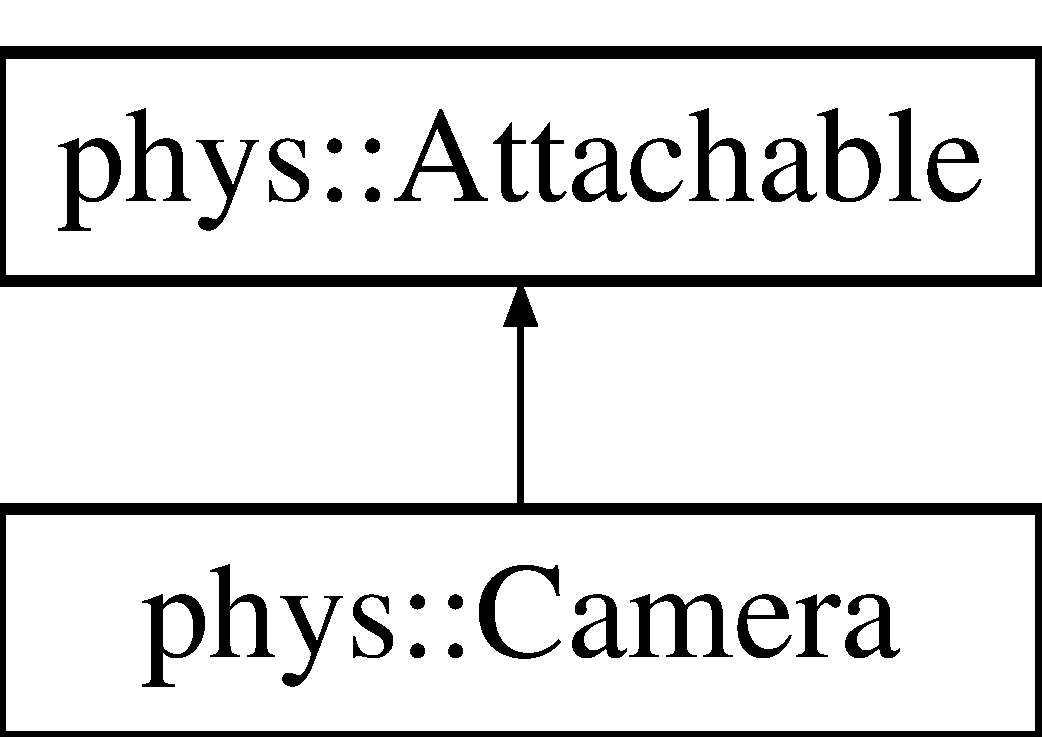
\includegraphics[height=2.000000cm]{classphys_1_1Camera}
\end{center}
\end{figure}
\subsubsection*{Public Types}
\begin{DoxyCompactItemize}
\item 
enum \hyperlink{classphys_1_1Camera_a87d8d46e9eb2080b10712079be69d86a}{ProjectionType} \{ \hyperlink{classphys_1_1Camera_a87d8d46e9eb2080b10712079be69d86aa6a71e6ab2139c8fc4d48d64aa9717f02}{Orthographic} =  0, 
\hyperlink{classphys_1_1Camera_a87d8d46e9eb2080b10712079be69d86aacfe21986c8c655b8d19ebd76118de055}{Perspective} =  1
 \}
\begin{DoxyCompactList}\small\item\em Values for storing how perspective should be interpretted. \item\end{DoxyCompactList}\end{DoxyCompactItemize}
\subsubsection*{Public Member Functions}
\begin{DoxyCompactItemize}
\item 
virtual void \hyperlink{classphys_1_1Camera_afaa81ebb01f1c64a324f802b6743b6f7}{AttachToFinal} (Ogre::SceneNode $\ast$RawTarget, \hyperlink{classphys_1_1WorldNode}{phys::WorldNode} $\ast$Target)
\begin{DoxyCompactList}\small\item\em Does the Final Work to attach on the \hyperlink{classphys_1_1Attachable}{Attachable} Side, should only be called by WorldNode::AttachFinal. \item\end{DoxyCompactList}\item 
\hyperlink{classphys_1_1Camera_a863e7b7a0fb4db7969014d8391b5ca30}{Camera} (const \hyperlink{namespacephys_aa03900411993de7fbfec4789bc1d392e}{String} \&Name, \hyperlink{classphys_1_1CameraManager}{CameraManager} $\ast$Manager)
\begin{DoxyCompactList}\small\item\em Basic \hyperlink{classphys_1_1Camera}{Camera} Constructor. \item\end{DoxyCompactList}\item 
\hyperlink{classphys_1_1Camera_a0510d4f9bf6fb195115272cbd116e8dd}{Camera} (Ogre::Camera $\ast$\hyperlink{classphys_1_1Camera}{Camera}, \hyperlink{classphys_1_1CameraManager}{CameraManager} $\ast$Manager)
\begin{DoxyCompactList}\small\item\em Ogre Cam Constructor. \item\end{DoxyCompactList}\item 
virtual void \hyperlink{classphys_1_1Camera_a087e4e09b4b0c7adf4c267c5e8e1a6d9}{DetachFromFinal} (Ogre::SceneNode $\ast$RawTarget)
\begin{DoxyCompactList}\small\item\em Does the Final Work to dettach on the Atachable Side, should only be called by WorldNode::DetachFinal. \item\end{DoxyCompactList}\item 
virtual \hyperlink{classphys_1_1Attachable_acd1fca033e7cc0bb3024a92d466d213a}{Attachable::AttachableElement} \hyperlink{classphys_1_1Camera_a4dce38bad69f1bc58f510ce01d6d6edf}{GetAttachableType} () const 
\begin{DoxyCompactList}\small\item\em What kind of \hyperlink{classphys_1_1Attachable}{Attachable} is this. \item\end{DoxyCompactList}\item 
\hyperlink{classphys_1_1Ray}{Ray} \hyperlink{classphys_1_1Camera_a01d119eb8bd10a8654493b043110ca0f}{GetCameraToViewportRay} (\hyperlink{namespacephys_af7eb897198d265b8e868f45240230d5f}{Real} Screenx, \hyperlink{namespacephys_af7eb897198d265b8e868f45240230d5f}{Real} Screeny) const 
\begin{DoxyCompactList}\small\item\em Gets a \hyperlink{classphys_1_1Ray}{Ray} from the camera to the viewport. \item\end{DoxyCompactList}\item 
\hyperlink{classphys_1_1Camera_a87d8d46e9eb2080b10712079be69d86a}{Camera::ProjectionType} \hyperlink{classphys_1_1Camera_aa79582e78a3eff11a8c4fe9c058566b0}{GetCameraType} () const 
\begin{DoxyCompactList}\small\item\em Get the type of projection used by the camera. \item\end{DoxyCompactList}\item 
\hyperlink{classphys_1_1Vector3}{Vector3} \hyperlink{classphys_1_1Camera_a6f0294569edb3e65de4139da361f83a9}{GetDirection} () const 
\begin{DoxyCompactList}\small\item\em Gets the direction the camera is currently facing. \item\end{DoxyCompactList}\item 
\hyperlink{classphys_1_1Vector3}{Vector3} \hyperlink{classphys_1_1Camera_a1f4126761e14d9b960395c79b6c4f13f}{GetFixedYawAxis} () const 
\begin{DoxyCompactList}\small\item\em If fixed yaw is enabled, on which axis is yawing disabled. \item\end{DoxyCompactList}\item 
\hyperlink{classphys_1_1Vector3}{Vector3} \hyperlink{classphys_1_1Camera_a7f71146cd533f6a1fc8426a9ed40b763}{GetGlobalLocation} () const 
\begin{DoxyCompactList}\small\item\em Gets the global/absolute location of the camera. \item\end{DoxyCompactList}\item 
virtual \hyperlink{classphys_1_1Vector3}{Vector3} \hyperlink{classphys_1_1Camera_a75b3f25ff664c4f95f0e04cb9edceeb4}{GetLocation} () const 
\item 
\hyperlink{namespacephys_a5ce5049f8b4bf88d6413c47b504ebb31}{ConstString} \& \hyperlink{classphys_1_1Camera_ae24490b8589796cb5f51d291cc418d84}{GetName} () const 
\begin{DoxyCompactList}\small\item\em Gets the camera's set name. \item\end{DoxyCompactList}\item 
Ogre::Camera $\ast$ \hyperlink{classphys_1_1Camera_a4f78f7a62580fa538d5bf2cb361644b2}{GetOgreCamera} () const 
\begin{DoxyCompactList}\small\item\em Gets the internal camera this camera is based on. \item\end{DoxyCompactList}\item 
\hyperlink{classphys_1_1Quaternion}{Quaternion} \hyperlink{classphys_1_1Camera_a48e0b33e0f12247bc0a0e0d6f759683e}{GetOrientation} () const 
\begin{DoxyCompactList}\small\item\em Gets the direction the camera is facing. \item\end{DoxyCompactList}\item 
\hyperlink{classphys_1_1Vector3}{Vector3} \hyperlink{classphys_1_1Camera_ae3dc70090e83e19a9c5f6df302bb57a5}{GetRelativeLocation} () const 
\begin{DoxyCompactList}\small\item\em Gets the relative location of the camera. \item\end{DoxyCompactList}\item 
bool \hyperlink{classphys_1_1Camera_a9b0aa17df46c427ab531bd587bd76e0f}{IsFixedYawEnabled} () const 
\begin{DoxyCompactList}\small\item\em Is fixed yaw enabled. \item\end{DoxyCompactList}\item 
void \hyperlink{classphys_1_1Camera_a299de2281cc566df476b4684ac7d89fa}{LookAt} (const \hyperlink{classphys_1_1Vector3}{Vector3} \&TargetLoc)
\begin{DoxyCompactList}\small\item\em Sets the direction the camera faces. \item\end{DoxyCompactList}\item 
void \hyperlink{classphys_1_1Camera_a63cce67b42008ee8ce481b1ffd7fcbdf}{Move} (const \hyperlink{classphys_1_1Vector3}{Vector3} \&ToMove)
\begin{DoxyCompactList}\small\item\em Moves the camera without factoring orientation. \item\end{DoxyCompactList}\item 
void \hyperlink{classphys_1_1Camera_a34a5a7b76016042ce8b2278c35437486}{MoveRelative} (const \hyperlink{classphys_1_1Vector3}{Vector3} \&ToMove)
\begin{DoxyCompactList}\small\item\em Moves the camera while factoring orientation. \item\end{DoxyCompactList}\item 
void \hyperlink{classphys_1_1Camera_a181465e6add36c07a63fdd26aee7c69a}{ResetZoom} ()
\begin{DoxyCompactList}\small\item\em Resets the zoom level back to the default. \item\end{DoxyCompactList}\item 
void \hyperlink{classphys_1_1Camera_a731d933c30bc95a83555412184d65cf8}{SetAspectRatio} (const \hyperlink{namespacephys_af7eb897198d265b8e868f45240230d5f}{Real} \&Ratio)
\begin{DoxyCompactList}\small\item\em Sets the aspect ratio of the cameras veiw. \item\end{DoxyCompactList}\item 
void \hyperlink{classphys_1_1Camera_a95d04ee7482ae6670229f59d63ee8926}{SetCameraType} (const \hyperlink{classphys_1_1Camera_a87d8d46e9eb2080b10712079be69d86a}{ProjectionType} Type)
\begin{DoxyCompactList}\small\item\em Sets the type of projection to be used with this camera. \item\end{DoxyCompactList}\item 
void \hyperlink{classphys_1_1Camera_a6ece06a179798b3240362b1bcb751f2f}{SetDirection} (const \hyperlink{classphys_1_1Vector3}{Vector3} \&Direction)
\begin{DoxyCompactList}\small\item\em Sets the Direction for the camera. \item\end{DoxyCompactList}\item 
void \hyperlink{classphys_1_1Camera_a77f0fa5cb6b934cfda8f5143afae3a0e}{SetFarClipDistance} (const \hyperlink{namespacephys_af7eb897198d265b8e868f45240230d5f}{Real} \&FarDist)
\begin{DoxyCompactList}\small\item\em Sets the long range clip distance. \item\end{DoxyCompactList}\item 
void \hyperlink{classphys_1_1Camera_a1b4d5be85c528541c7a1cbebb41bfd89}{SetFixedYawAxis} (bool UseFixed)
\begin{DoxyCompactList}\small\item\em Sets whether to lock rotation around the Y axis. \item\end{DoxyCompactList}\item 
void \hyperlink{classphys_1_1Camera_aa6d7285b7a3fc43e3c6dd05ff30f89ab}{SetFixedYawAxis} (bool UseFixed, const \hyperlink{classphys_1_1Vector3}{Vector3} \&Axis)
\begin{DoxyCompactList}\small\item\em Sets whether to lock rotation around the Y axis. \item\end{DoxyCompactList}\item 
virtual void \hyperlink{classphys_1_1Camera_afd2a77e96dd6d0dec1071dcc3229425f}{SetLocation} (const \hyperlink{classphys_1_1Vector3}{Vector3} \&Location)
\begin{DoxyCompactList}\small\item\em Sets the location of a camera. \item\end{DoxyCompactList}\item 
void \hyperlink{classphys_1_1Camera_a0fdf28666baba46e907d6a8eac714915}{SetNearClipDistance} (const \hyperlink{namespacephys_af7eb897198d265b8e868f45240230d5f}{Real} \&NearDist)
\begin{DoxyCompactList}\small\item\em Sets the short range clip distance. \item\end{DoxyCompactList}\item 
void \hyperlink{classphys_1_1Camera_adbfa4a59eb09c0578c9aac792b78ef55}{SetOrientation} (const \hyperlink{classphys_1_1Quaternion}{Quaternion} \&Orientation)
\begin{DoxyCompactList}\small\item\em Sets the orientation of the camera. \item\end{DoxyCompactList}\item 
void \hyperlink{classphys_1_1Camera_a24cb50ccb644f3f7e925819aba3ddad2}{SetOrthoWindow} (const \hyperlink{namespacephys_af7eb897198d265b8e868f45240230d5f}{Real} \&Width, const \hyperlink{namespacephys_af7eb897198d265b8e868f45240230d5f}{Real} \&Height)
\begin{DoxyCompactList}\small\item\em Defines the size of the Orthographic projection window. \item\end{DoxyCompactList}\item 
void \hyperlink{classphys_1_1Camera_a76c140a73a4d862f260b4a76d85b4e34}{SetOrthoWindowHeight} (const \hyperlink{namespacephys_af7eb897198d265b8e868f45240230d5f}{Real} \&Height)
\begin{DoxyCompactList}\small\item\em Defines the size of the Orthographic projection window. \item\end{DoxyCompactList}\item 
void \hyperlink{classphys_1_1Camera_a1e5ba572ce27880def46538157f4ccb7}{SetOrthoWindowWidth} (const \hyperlink{namespacephys_af7eb897198d265b8e868f45240230d5f}{Real} \&Width)
\begin{DoxyCompactList}\small\item\em Defines the size of the Orthographic projection window. \item\end{DoxyCompactList}\item 
void \hyperlink{classphys_1_1Camera_a66e2854557687d98cc5882363e6d6606}{ZoomCamera} (const \hyperlink{namespacephys_af7eb897198d265b8e868f45240230d5f}{Real} \&Zoom)
\begin{DoxyCompactList}\small\item\em Will zoom in or out the camera. \item\end{DoxyCompactList}\item 
virtual \hyperlink{classphys_1_1Camera_aa45f340a6f7ba0970aa2602a928463ea}{$\sim$Camera} ()
\begin{DoxyCompactList}\small\item\em Class Destructor. \item\end{DoxyCompactList}\end{DoxyCompactItemize}
\subsubsection*{Protected Attributes}
\begin{DoxyCompactItemize}
\item 
\hypertarget{classphys_1_1Camera_a91622148b9b9a9ae1554c828f7e2fc89}{
Ogre::Camera $\ast$ \hyperlink{classphys_1_1Camera_a91622148b9b9a9ae1554c828f7e2fc89}{Cam}}
\label{classphys_1_1Camera_a91622148b9b9a9ae1554c828f7e2fc89}

\begin{DoxyCompactList}\small\item\em This is the \hyperlink{classphys_1_1Camera}{Camera} used by the graphics Subsystem, that this class wraps. \item\end{DoxyCompactList}\item 
\hypertarget{classphys_1_1Camera_a909203ede748deb1b587a8758ba8cec4}{
\hyperlink{classphys_1_1CameraManager}{CameraManager} $\ast$ \hyperlink{classphys_1_1Camera_a909203ede748deb1b587a8758ba8cec4}{CamManager}}
\label{classphys_1_1Camera_a909203ede748deb1b587a8758ba8cec4}

\begin{DoxyCompactList}\small\item\em This is the \hyperlink{classphys_1_1Camera}{Camera} manager that this camera is attached to. \item\end{DoxyCompactList}\end{DoxyCompactItemize}
\subsubsection*{Friends}
\begin{DoxyCompactItemize}
\item 
\hypertarget{classphys_1_1Camera_afae5bf9a900e8c5bc70c9332785e8465}{
class {\bfseries CameraManager}}
\label{classphys_1_1Camera_afae5bf9a900e8c5bc70c9332785e8465}

\item 
\hypertarget{classphys_1_1Camera_a903516ddc793b1d17d4d766a13bd6962}{
\hyperlink{classphys_1_1xml_1_1Node}{xml::Node} \&PHYS\_\-LIB {\bfseries operator$>$$>$} (\hyperlink{classphys_1_1xml_1_1Node}{xml::Node} \&OneNode, \hyperlink{classphys_1_1Camera}{Camera} \&Ev)}
\label{classphys_1_1Camera_a903516ddc793b1d17d4d766a13bd6962}

\end{DoxyCompactItemize}


\subsubsection{Detailed Description}
This is the camera class. This class contains all the functionality needed to manipulate an individual camera that has been created. \begin{Desc}
\item[\hyperlink{todo__todo000002}{Todo}]Fix all the extra occurences of the word \hyperlink{classphys_1_1Camera}{Camera} in Function names on the camera. \end{Desc}


Definition at line 102 of file camera.h.



\subsubsection{Member Enumeration Documentation}
\hypertarget{classphys_1_1Camera_a87d8d46e9eb2080b10712079be69d86a}{
\index{phys::Camera@{phys::Camera}!ProjectionType@{ProjectionType}}
\index{ProjectionType@{ProjectionType}!phys::Camera@{phys::Camera}}
\paragraph[{ProjectionType}]{\setlength{\rightskip}{0pt plus 5cm}enum {\bf phys::Camera::ProjectionType}}\hfill}
\label{classphys_1_1Camera_a87d8d46e9eb2080b10712079be69d86a}


Values for storing how perspective should be interpretted. 

\begin{Desc}
\item[Enumerator: ]\par
\begin{description}
\index{Orthographic@{Orthographic}!phys::Camera@{phys::Camera}}\index{phys::Camera@{phys::Camera}!Orthographic@{Orthographic}}\item[{\em 
\hypertarget{classphys_1_1Camera_a87d8d46e9eb2080b10712079be69d86aa6a71e6ab2139c8fc4d48d64aa9717f02}{
Orthographic}
\label{classphys_1_1Camera_a87d8d46e9eb2080b10712079be69d86aa6a71e6ab2139c8fc4d48d64aa9717f02}
}]Not at all, objects at any distance are the same size. \index{Perspective@{Perspective}!phys::Camera@{phys::Camera}}\index{phys::Camera@{phys::Camera}!Perspective@{Perspective}}\item[{\em 
\hypertarget{classphys_1_1Camera_a87d8d46e9eb2080b10712079be69d86aacfe21986c8c655b8d19ebd76118de055}{
Perspective}
\label{classphys_1_1Camera_a87d8d46e9eb2080b10712079be69d86aacfe21986c8c655b8d19ebd76118de055}
}]Normal perspective. \end{description}
\end{Desc}



Definition at line 106 of file camera.h.



\subsubsection{Constructor \& Destructor Documentation}
\hypertarget{classphys_1_1Camera_a863e7b7a0fb4db7969014d8391b5ca30}{
\index{phys::Camera@{phys::Camera}!Camera@{Camera}}
\index{Camera@{Camera}!phys::Camera@{phys::Camera}}
\paragraph[{Camera}]{\setlength{\rightskip}{0pt plus 5cm}phys::Camera::Camera (
\begin{DoxyParamCaption}
\item[{const {\bf String} \&}]{Name, }
\item[{{\bf CameraManager} $\ast$}]{Manager}
\end{DoxyParamCaption}
)}\hfill}
\label{classphys_1_1Camera_a863e7b7a0fb4db7969014d8391b5ca30}


Basic \hyperlink{classphys_1_1Camera}{Camera} Constructor. 

This is the basic constructor for the \hyperlink{classphys_1_1Camera}{Camera} class. 

Definition at line 60 of file camera.cpp.

\hypertarget{classphys_1_1Camera_a0510d4f9bf6fb195115272cbd116e8dd}{
\index{phys::Camera@{phys::Camera}!Camera@{Camera}}
\index{Camera@{Camera}!phys::Camera@{phys::Camera}}
\paragraph[{Camera}]{\setlength{\rightskip}{0pt plus 5cm}phys::Camera::Camera (
\begin{DoxyParamCaption}
\item[{Ogre::Camera $\ast$}]{Camera, }
\item[{{\bf CameraManager} $\ast$}]{Manager}
\end{DoxyParamCaption}
)}\hfill}
\label{classphys_1_1Camera_a0510d4f9bf6fb195115272cbd116e8dd}


Ogre Cam Constructor. 

This is for internal use only and shouldn't be called manually. 

Definition at line 66 of file camera.cpp.

\hypertarget{classphys_1_1Camera_aa45f340a6f7ba0970aa2602a928463ea}{
\index{phys::Camera@{phys::Camera}!$\sim$Camera@{$\sim$Camera}}
\index{$\sim$Camera@{$\sim$Camera}!phys::Camera@{phys::Camera}}
\paragraph[{$\sim$Camera}]{\setlength{\rightskip}{0pt plus 5cm}phys::Camera::$\sim$Camera (
\begin{DoxyParamCaption}
{}
\end{DoxyParamCaption}
)\hspace{0.3cm}{\ttfamily  \mbox{[}virtual\mbox{]}}}\hfill}
\label{classphys_1_1Camera_aa45f340a6f7ba0970aa2602a928463ea}


Class Destructor. 

The Class Destructor. 

Definition at line 80 of file camera.cpp.



\subsubsection{Member Function Documentation}
\hypertarget{classphys_1_1Camera_afaa81ebb01f1c64a324f802b6743b6f7}{
\index{phys::Camera@{phys::Camera}!AttachToFinal@{AttachToFinal}}
\index{AttachToFinal@{AttachToFinal}!phys::Camera@{phys::Camera}}
\paragraph[{AttachToFinal}]{\setlength{\rightskip}{0pt plus 5cm}void phys::Camera::AttachToFinal (
\begin{DoxyParamCaption}
\item[{Ogre::SceneNode $\ast$}]{RawTarget, }
\item[{{\bf phys::WorldNode} $\ast$}]{Target}
\end{DoxyParamCaption}
)\hspace{0.3cm}{\ttfamily  \mbox{[}virtual\mbox{]}}}\hfill}
\label{classphys_1_1Camera_afaa81ebb01f1c64a324f802b6743b6f7}


Does the Final Work to attach on the \hyperlink{classphys_1_1Attachable}{Attachable} Side, should only be called by WorldNode::AttachFinal. 


\begin{DoxyParams}{Parameters}
{\em RawTarget} & Any Raw data that need to be passed to finalize attaching \\
\hline
{\em Target} & a pointer to the Worldnode being attached to.\\
\hline
\end{DoxyParams}
This Sets the attaching pointer appropriately, This must be done if overiding this functioning. Any other specific items relating directly to attaching should happen here. In general other attaching dependent behaviors should not go here. This is called from \hyperlink{classphys_1_1WorldNode_a6e4aa8bc4b916cfff06d03814a7dd80f}{WorldNode::AttachObjectFinal()}. 

Reimplemented from \hyperlink{classphys_1_1Attachable_a77c8234874f53b159f4156c0c984fad0}{phys::Attachable}.



Definition at line 266 of file camera.cpp.

\hypertarget{classphys_1_1Camera_a087e4e09b4b0c7adf4c267c5e8e1a6d9}{
\index{phys::Camera@{phys::Camera}!DetachFromFinal@{DetachFromFinal}}
\index{DetachFromFinal@{DetachFromFinal}!phys::Camera@{phys::Camera}}
\paragraph[{DetachFromFinal}]{\setlength{\rightskip}{0pt plus 5cm}void phys::Camera::DetachFromFinal (
\begin{DoxyParamCaption}
\item[{Ogre::SceneNode $\ast$}]{RawTarget}
\end{DoxyParamCaption}
)\hspace{0.3cm}{\ttfamily  \mbox{[}virtual\mbox{]}}}\hfill}
\label{classphys_1_1Camera_a087e4e09b4b0c7adf4c267c5e8e1a6d9}


Does the Final Work to dettach on the Atachable Side, should only be called by WorldNode::DetachFinal. 

This Sets the attached pointer to 0, This must be done if overiding this functioning. Any other specific items relating directly to detaching should happen here. In general other detaching dependent behaviors should not go here. This is called from \hyperlink{classphys_1_1WorldNode_ae300db6515b782b165e77d19b7137851}{WorldNode::DetachObjectFinal()}. 
\begin{DoxyParams}{Parameters}
{\em RawTarget} & Any Raw data that need to be passed to finalize detaching \\
\hline
\end{DoxyParams}


Reimplemented from \hyperlink{classphys_1_1Attachable_a3e4d8113c4b45ece63c29180cf96029a}{phys::Attachable}.



Definition at line 272 of file camera.cpp.

\hypertarget{classphys_1_1Camera_a4dce38bad69f1bc58f510ce01d6d6edf}{
\index{phys::Camera@{phys::Camera}!GetAttachableType@{GetAttachableType}}
\index{GetAttachableType@{GetAttachableType}!phys::Camera@{phys::Camera}}
\paragraph[{GetAttachableType}]{\setlength{\rightskip}{0pt plus 5cm}{\bf Attachable::AttachableElement} phys::Camera::GetAttachableType (
\begin{DoxyParamCaption}
{}
\end{DoxyParamCaption}
) const\hspace{0.3cm}{\ttfamily  \mbox{[}virtual\mbox{]}}}\hfill}
\label{classphys_1_1Camera_a4dce38bad69f1bc58f510ce01d6d6edf}


What kind of \hyperlink{classphys_1_1Attachable}{Attachable} is this. 

Inherited From \hyperlink{classphys_1_1Attachable}{Attachable} \begin{DoxyReturn}{Returns}
An \hyperlink{classphys_1_1Attachable_a1c84342fe19d8eef33de4789e19c9d00}{Attachable::GetAttachableType} containing \hyperlink{classphys_1_1Attachable_acd1fca033e7cc0bb3024a92d466d213aa8de5bba9ffca8ba85776e5a54eb26654}{Attachable::Camera}.
\end{DoxyReturn}
Inherited From \hyperlink{classphys_1_1Attachable}{Attachable} 

Implements \hyperlink{classphys_1_1Attachable_a1c84342fe19d8eef33de4789e19c9d00}{phys::Attachable}.



Definition at line 263 of file camera.cpp.

\hypertarget{classphys_1_1Camera_a01d119eb8bd10a8654493b043110ca0f}{
\index{phys::Camera@{phys::Camera}!GetCameraToViewportRay@{GetCameraToViewportRay}}
\index{GetCameraToViewportRay@{GetCameraToViewportRay}!phys::Camera@{phys::Camera}}
\paragraph[{GetCameraToViewportRay}]{\setlength{\rightskip}{0pt plus 5cm}{\bf Ray} phys::Camera::GetCameraToViewportRay (
\begin{DoxyParamCaption}
\item[{{\bf Real}}]{Screenx, }
\item[{{\bf Real}}]{Screeny}
\end{DoxyParamCaption}
) const}\hfill}
\label{classphys_1_1Camera_a01d119eb8bd10a8654493b043110ca0f}


Gets a \hyperlink{classphys_1_1Ray}{Ray} from the camera to the viewport. 

This will cast a ray from the camera to the viewport and return it. 
\begin{DoxyParams}{Parameters}
{\em Screenx} & A Real representing the relative location on screen, on the x axis(0.0-\/1.0). \\
\hline
{\em Screeny} & A Real representing the relative location on screen, on the y axis(0.0-\/1.0). \\
\hline
\end{DoxyParams}


Definition at line 215 of file camera.cpp.

\hypertarget{classphys_1_1Camera_aa79582e78a3eff11a8c4fe9c058566b0}{
\index{phys::Camera@{phys::Camera}!GetCameraType@{GetCameraType}}
\index{GetCameraType@{GetCameraType}!phys::Camera@{phys::Camera}}
\paragraph[{GetCameraType}]{\setlength{\rightskip}{0pt plus 5cm}{\bf Camera::ProjectionType} phys::Camera::GetCameraType (
\begin{DoxyParamCaption}
{}
\end{DoxyParamCaption}
) const}\hfill}
\label{classphys_1_1Camera_aa79582e78a3eff11a8c4fe9c058566b0}


Get the type of projection used by the camera. 

\begin{DoxyReturn}{Returns}
A ProjectionType that will identify the kind of projection this camera uses. 
\end{DoxyReturn}


Definition at line 105 of file camera.cpp.

\hypertarget{classphys_1_1Camera_a6f0294569edb3e65de4139da361f83a9}{
\index{phys::Camera@{phys::Camera}!GetDirection@{GetDirection}}
\index{GetDirection@{GetDirection}!phys::Camera@{phys::Camera}}
\paragraph[{GetDirection}]{\setlength{\rightskip}{0pt plus 5cm}{\bf Vector3} phys::Camera::GetDirection (
\begin{DoxyParamCaption}
{}
\end{DoxyParamCaption}
) const}\hfill}
\label{classphys_1_1Camera_a6f0294569edb3e65de4139da361f83a9}


Gets the direction the camera is currently facing. 

\begin{DoxyReturn}{Returns}
Returns a \hyperlink{classphys_1_1Vector3}{Vector3} representing the current direction the camera is facing. 
\end{DoxyReturn}
\hypertarget{classphys_1_1Camera_a1f4126761e14d9b960395c79b6c4f13f}{
\index{phys::Camera@{phys::Camera}!GetFixedYawAxis@{GetFixedYawAxis}}
\index{GetFixedYawAxis@{GetFixedYawAxis}!phys::Camera@{phys::Camera}}
\paragraph[{GetFixedYawAxis}]{\setlength{\rightskip}{0pt plus 5cm}{\bf Vector3} phys::Camera::GetFixedYawAxis (
\begin{DoxyParamCaption}
{}
\end{DoxyParamCaption}
) const}\hfill}
\label{classphys_1_1Camera_a1f4126761e14d9b960395c79b6c4f13f}


If fixed yaw is enabled, on which axis is yawing disabled. 

\begin{DoxyReturn}{Returns}
Returns a \hyperlink{classphys_1_1Vector3}{Vector3} of 0s if disable, otherwise this return the Fixed Yaw Axis. 
\end{DoxyReturn}


Definition at line 195 of file camera.cpp.

\hypertarget{classphys_1_1Camera_a7f71146cd533f6a1fc8426a9ed40b763}{
\index{phys::Camera@{phys::Camera}!GetGlobalLocation@{GetGlobalLocation}}
\index{GetGlobalLocation@{GetGlobalLocation}!phys::Camera@{phys::Camera}}
\paragraph[{GetGlobalLocation}]{\setlength{\rightskip}{0pt plus 5cm}{\bf Vector3} phys::Camera::GetGlobalLocation (
\begin{DoxyParamCaption}
{}
\end{DoxyParamCaption}
) const}\hfill}
\label{classphys_1_1Camera_a7f71146cd533f6a1fc8426a9ed40b763}


Gets the global/absolute location of the camera. 

\begin{DoxyReturn}{Returns}
A \hyperlink{classphys_1_1Vector3}{phys::Vector3} containing the location of this object as an offset from the global origin. 
\end{DoxyReturn}


Definition at line 233 of file camera.cpp.

\hypertarget{classphys_1_1Camera_a75b3f25ff664c4f95f0e04cb9edceeb4}{
\index{phys::Camera@{phys::Camera}!GetLocation@{GetLocation}}
\index{GetLocation@{GetLocation}!phys::Camera@{phys::Camera}}
\paragraph[{GetLocation}]{\setlength{\rightskip}{0pt plus 5cm}{\bf Vector3} phys::Camera::GetLocation (
\begin{DoxyParamCaption}
{}
\end{DoxyParamCaption}
) const\hspace{0.3cm}{\ttfamily  \mbox{[}virtual\mbox{]}}}\hfill}
\label{classphys_1_1Camera_a75b3f25ff664c4f95f0e04cb9edceeb4}
Gets the location of the camera, relative to any parent \hyperlink{classphys_1_1WorldNode}{WorldNode}. \begin{DoxyReturn}{Returns}
A \hyperlink{classphys_1_1Vector3}{phys::Vector3} with the location of the camera as though the Parent \hyperlink{classphys_1_1WorldNode}{WorldNode} were the origin. 
\end{DoxyReturn}


Implements \hyperlink{classphys_1_1Attachable_acb410686b2719524eb484b50cc9054a4}{phys::Attachable}.



Definition at line 227 of file camera.cpp.

\hypertarget{classphys_1_1Camera_ae24490b8589796cb5f51d291cc418d84}{
\index{phys::Camera@{phys::Camera}!GetName@{GetName}}
\index{GetName@{GetName}!phys::Camera@{phys::Camera}}
\paragraph[{GetName}]{\setlength{\rightskip}{0pt plus 5cm}{\bf ConstString} \& phys::Camera::GetName (
\begin{DoxyParamCaption}
{}
\end{DoxyParamCaption}
) const\hspace{0.3cm}{\ttfamily  \mbox{[}virtual\mbox{]}}}\hfill}
\label{classphys_1_1Camera_ae24490b8589796cb5f51d291cc418d84}


Gets the camera's set name. 

\begin{DoxyReturn}{Returns}
Returns a string containing the camera's name. 
\end{DoxyReturn}


Implements \hyperlink{classphys_1_1Attachable_a0a07d727fa2630dc3550fd991ca28256}{phys::Attachable}.



Definition at line 86 of file camera.cpp.

\hypertarget{classphys_1_1Camera_a4f78f7a62580fa538d5bf2cb361644b2}{
\index{phys::Camera@{phys::Camera}!GetOgreCamera@{GetOgreCamera}}
\index{GetOgreCamera@{GetOgreCamera}!phys::Camera@{phys::Camera}}
\paragraph[{GetOgreCamera}]{\setlength{\rightskip}{0pt plus 5cm}Ogre::Camera $\ast$ phys::Camera::GetOgreCamera (
\begin{DoxyParamCaption}
{}
\end{DoxyParamCaption}
) const}\hfill}
\label{classphys_1_1Camera_a4f78f7a62580fa538d5bf2cb361644b2}


Gets the internal camera this camera is based on. 

\begin{DoxyReturn}{Returns}
Returns a pointer to the Ogre \hyperlink{classphys_1_1Camera}{Camera} this camera is based on. 
\end{DoxyReturn}


Definition at line 256 of file camera.cpp.

\hypertarget{classphys_1_1Camera_a48e0b33e0f12247bc0a0e0d6f759683e}{
\index{phys::Camera@{phys::Camera}!GetOrientation@{GetOrientation}}
\index{GetOrientation@{GetOrientation}!phys::Camera@{phys::Camera}}
\paragraph[{GetOrientation}]{\setlength{\rightskip}{0pt plus 5cm}{\bf Quaternion} phys::Camera::GetOrientation (
\begin{DoxyParamCaption}
{}
\end{DoxyParamCaption}
) const}\hfill}
\label{classphys_1_1Camera_a48e0b33e0f12247bc0a0e0d6f759683e}


Gets the direction the camera is facing. 

\begin{DoxyReturn}{Returns}
A \hyperlink{classphys_1_1Quaternion}{phys::Quaternion} representing how the camera is rotated. 
\end{DoxyReturn}


Definition at line 236 of file camera.cpp.

\hypertarget{classphys_1_1Camera_ae3dc70090e83e19a9c5f6df302bb57a5}{
\index{phys::Camera@{phys::Camera}!GetRelativeLocation@{GetRelativeLocation}}
\index{GetRelativeLocation@{GetRelativeLocation}!phys::Camera@{phys::Camera}}
\paragraph[{GetRelativeLocation}]{\setlength{\rightskip}{0pt plus 5cm}{\bf Vector3} phys::Camera::GetRelativeLocation (
\begin{DoxyParamCaption}
{}
\end{DoxyParamCaption}
) const}\hfill}
\label{classphys_1_1Camera_ae3dc70090e83e19a9c5f6df302bb57a5}


Gets the relative location of the camera. 

Gets the location of the camera, relative to any parent \hyperlink{classphys_1_1WorldNode}{WorldNode}. \begin{DoxyReturn}{Returns}
A \hyperlink{classphys_1_1Vector3}{phys::Vector3} with the location of the camera as though the Parent \hyperlink{classphys_1_1WorldNode}{WorldNode} were the origin. 
\end{DoxyReturn}


Definition at line 230 of file camera.cpp.

\hypertarget{classphys_1_1Camera_a9b0aa17df46c427ab531bd587bd76e0f}{
\index{phys::Camera@{phys::Camera}!IsFixedYawEnabled@{IsFixedYawEnabled}}
\index{IsFixedYawEnabled@{IsFixedYawEnabled}!phys::Camera@{phys::Camera}}
\paragraph[{IsFixedYawEnabled}]{\setlength{\rightskip}{0pt plus 5cm}bool phys::Camera::IsFixedYawEnabled (
\begin{DoxyParamCaption}
{}
\end{DoxyParamCaption}
) const}\hfill}
\label{classphys_1_1Camera_a9b0aa17df46c427ab531bd587bd76e0f}


Is fixed yaw enabled. 

\begin{DoxyReturn}{Returns}
True if it is enable, such as the default setting, or false if it is not enabled. 
\end{DoxyReturn}


Definition at line 192 of file camera.cpp.

\hypertarget{classphys_1_1Camera_a299de2281cc566df476b4684ac7d89fa}{
\index{phys::Camera@{phys::Camera}!LookAt@{LookAt}}
\index{LookAt@{LookAt}!phys::Camera@{phys::Camera}}
\paragraph[{LookAt}]{\setlength{\rightskip}{0pt plus 5cm}void phys::Camera::LookAt (
\begin{DoxyParamCaption}
\item[{const {\bf Vector3} \&}]{TargetLoc}
\end{DoxyParamCaption}
)}\hfill}
\label{classphys_1_1Camera_a299de2281cc566df476b4684ac7d89fa}


Sets the direction the camera faces. 

Sets the direction the camera faces. Will also take orientation into account. 
\begin{DoxyParams}{Parameters}
{\em TargetLoc} & The location in the game world to look at. \\
\hline
\end{DoxyParams}


Definition at line 164 of file camera.cpp.

\hypertarget{classphys_1_1Camera_a63cce67b42008ee8ce481b1ffd7fcbdf}{
\index{phys::Camera@{phys::Camera}!Move@{Move}}
\index{Move@{Move}!phys::Camera@{phys::Camera}}
\paragraph[{Move}]{\setlength{\rightskip}{0pt plus 5cm}void phys::Camera::Move (
\begin{DoxyParamCaption}
\item[{const {\bf Vector3} \&}]{ToMove}
\end{DoxyParamCaption}
)}\hfill}
\label{classphys_1_1Camera_a63cce67b42008ee8ce481b1ffd7fcbdf}


Moves the camera without factoring orientation. 

This function will move the camera along the provided vector based on world axes. 
\begin{DoxyParams}{Parameters}
{\em ToMove} & The vector to move the camera by. \\
\hline
\end{DoxyParams}


Definition at line 169 of file camera.cpp.

\hypertarget{classphys_1_1Camera_a34a5a7b76016042ce8b2278c35437486}{
\index{phys::Camera@{phys::Camera}!MoveRelative@{MoveRelative}}
\index{MoveRelative@{MoveRelative}!phys::Camera@{phys::Camera}}
\paragraph[{MoveRelative}]{\setlength{\rightskip}{0pt plus 5cm}void phys::Camera::MoveRelative (
\begin{DoxyParamCaption}
\item[{const {\bf Vector3} \&}]{ToMove}
\end{DoxyParamCaption}
)}\hfill}
\label{classphys_1_1Camera_a34a5a7b76016042ce8b2278c35437486}


Moves the camera while factoring orientation. 

This function will move the camera along the provided vector based on local axes. 
\begin{DoxyParams}{Parameters}
{\em ToMove} & The vector to move the camera by. \\
\hline
\end{DoxyParams}


Definition at line 174 of file camera.cpp.

\hypertarget{classphys_1_1Camera_a181465e6add36c07a63fdd26aee7c69a}{
\index{phys::Camera@{phys::Camera}!ResetZoom@{ResetZoom}}
\index{ResetZoom@{ResetZoom}!phys::Camera@{phys::Camera}}
\paragraph[{ResetZoom}]{\setlength{\rightskip}{0pt plus 5cm}void phys::Camera::ResetZoom (
\begin{DoxyParamCaption}
{}
\end{DoxyParamCaption}
)}\hfill}
\label{classphys_1_1Camera_a181465e6add36c07a63fdd26aee7c69a}


Resets the zoom level back to the default. 

This function will return the zoom level back to normal. Note this function will only work if the camera is attached to a node. 

Definition at line 247 of file camera.cpp.

\hypertarget{classphys_1_1Camera_a731d933c30bc95a83555412184d65cf8}{
\index{phys::Camera@{phys::Camera}!SetAspectRatio@{SetAspectRatio}}
\index{SetAspectRatio@{SetAspectRatio}!phys::Camera@{phys::Camera}}
\paragraph[{SetAspectRatio}]{\setlength{\rightskip}{0pt plus 5cm}void phys::Camera::SetAspectRatio (
\begin{DoxyParamCaption}
\item[{const {\bf Real} \&}]{Ratio}
\end{DoxyParamCaption}
)}\hfill}
\label{classphys_1_1Camera_a731d933c30bc95a83555412184d65cf8}


Sets the aspect ratio of the cameras veiw. 

This function will set the aspect ratio between the width and height of the cameras viewing area. 
\begin{DoxyParams}{Parameters}
{\em Ratio} & A Real that represents the aspect ratio, where Ratio = width / height. \\
\hline
\end{DoxyParams}


Definition at line 159 of file camera.cpp.

\hypertarget{classphys_1_1Camera_a95d04ee7482ae6670229f59d63ee8926}{
\index{phys::Camera@{phys::Camera}!SetCameraType@{SetCameraType}}
\index{SetCameraType@{SetCameraType}!phys::Camera@{phys::Camera}}
\paragraph[{SetCameraType}]{\setlength{\rightskip}{0pt plus 5cm}void phys::Camera::SetCameraType (
\begin{DoxyParamCaption}
\item[{const {\bf ProjectionType}}]{Type}
\end{DoxyParamCaption}
)}\hfill}
\label{classphys_1_1Camera_a95d04ee7482ae6670229f59d63ee8926}


Sets the type of projection to be used with this camera. 

By default, all cameras are enabled with Perspective projection. This is the standard 3-\/dimentional view anyone would expect in a 3D world. Orthographic projection is useful when displaying 2D worlds, or only 2 dimentions of a 3D world. It enables you to see the entire side of an object without regard for camera perspective. Perspective can be thought of as a pyramid, with the camera at the top of the cone. Orthographic would instead be a cube. 
\begin{DoxyParams}{Parameters}
{\em Type} & The type of projection to be used. \\
\hline
\end{DoxyParams}


Definition at line 91 of file camera.cpp.

\hypertarget{classphys_1_1Camera_a6ece06a179798b3240362b1bcb751f2f}{
\index{phys::Camera@{phys::Camera}!SetDirection@{SetDirection}}
\index{SetDirection@{SetDirection}!phys::Camera@{phys::Camera}}
\paragraph[{SetDirection}]{\setlength{\rightskip}{0pt plus 5cm}void phys::Camera::SetDirection (
\begin{DoxyParamCaption}
\item[{const {\bf Vector3} \&}]{Direction}
\end{DoxyParamCaption}
)}\hfill}
\label{classphys_1_1Camera_a6ece06a179798b3240362b1bcb751f2f}


Sets the Direction for the camera. 

Sets which axis the camera will look down for rendering. 
\begin{DoxyParams}{Parameters}
{\em Direction} & The vector3 representing the axis to be used. \\
\hline
\end{DoxyParams}


Definition at line 139 of file camera.cpp.

\hypertarget{classphys_1_1Camera_a77f0fa5cb6b934cfda8f5143afae3a0e}{
\index{phys::Camera@{phys::Camera}!SetFarClipDistance@{SetFarClipDistance}}
\index{SetFarClipDistance@{SetFarClipDistance}!phys::Camera@{phys::Camera}}
\paragraph[{SetFarClipDistance}]{\setlength{\rightskip}{0pt plus 5cm}void phys::Camera::SetFarClipDistance (
\begin{DoxyParamCaption}
\item[{const {\bf Real} \&}]{FarDist}
\end{DoxyParamCaption}
)}\hfill}
\label{classphys_1_1Camera_a77f0fa5cb6b934cfda8f5143afae3a0e}


Sets the long range clip distance. 

Sets the distance at which objects are considered too far to render. 
\begin{DoxyParams}{Parameters}
{\em FarDist} & A Real representing the distance. Note: This number directly corolates to the dimentions you provide in the constructor for the physgame. You should understand your games scale before setting this number. \\
\hline
\end{DoxyParams}


Definition at line 154 of file camera.cpp.

\hypertarget{classphys_1_1Camera_aa6d7285b7a3fc43e3c6dd05ff30f89ab}{
\index{phys::Camera@{phys::Camera}!SetFixedYawAxis@{SetFixedYawAxis}}
\index{SetFixedYawAxis@{SetFixedYawAxis}!phys::Camera@{phys::Camera}}
\paragraph[{SetFixedYawAxis}]{\setlength{\rightskip}{0pt plus 5cm}void phys::Camera::SetFixedYawAxis (
\begin{DoxyParamCaption}
\item[{bool}]{UseFixed, }
\item[{const {\bf Vector3} \&}]{Axis}
\end{DoxyParamCaption}
)}\hfill}
\label{classphys_1_1Camera_aa6d7285b7a3fc43e3c6dd05ff30f89ab}


Sets whether to lock rotation around the Y axis. 

This function will lock rotations around the Y axis (or another axis if you specify). This function is automatically called on by the camera constructor. 
\begin{DoxyParams}{Parameters}
{\em UseFixed} & Enable or disable the locking of the axis. \\
\hline
{\em Axis} & The axis to lock, defaults to the Y axis. \\
\hline
\end{DoxyParams}


Definition at line 179 of file camera.cpp.

\hypertarget{classphys_1_1Camera_a1b4d5be85c528541c7a1cbebb41bfd89}{
\index{phys::Camera@{phys::Camera}!SetFixedYawAxis@{SetFixedYawAxis}}
\index{SetFixedYawAxis@{SetFixedYawAxis}!phys::Camera@{phys::Camera}}
\paragraph[{SetFixedYawAxis}]{\setlength{\rightskip}{0pt plus 5cm}void phys::Camera::SetFixedYawAxis (
\begin{DoxyParamCaption}
\item[{bool}]{UseFixed}
\end{DoxyParamCaption}
)}\hfill}
\label{classphys_1_1Camera_a1b4d5be85c528541c7a1cbebb41bfd89}


Sets whether to lock rotation around the Y axis. 

This function will lock rotations around the Y axis. This function is automatically called on by the camera constructor to enable camera yawing. 
\begin{DoxyParams}{Parameters}
{\em UseFixed} & Enable or disable the locking of the axis. \\
\hline
\end{DoxyParams}


Definition at line 186 of file camera.cpp.

\hypertarget{classphys_1_1Camera_afd2a77e96dd6d0dec1071dcc3229425f}{
\index{phys::Camera@{phys::Camera}!SetLocation@{SetLocation}}
\index{SetLocation@{SetLocation}!phys::Camera@{phys::Camera}}
\paragraph[{SetLocation}]{\setlength{\rightskip}{0pt plus 5cm}void phys::Camera::SetLocation (
\begin{DoxyParamCaption}
\item[{const {\bf Vector3} \&}]{Location}
\end{DoxyParamCaption}
)\hspace{0.3cm}{\ttfamily  \mbox{[}virtual\mbox{]}}}\hfill}
\label{classphys_1_1Camera_afd2a77e96dd6d0dec1071dcc3229425f}


Sets the location of a camera. 

Sets the location of the specified camera. 
\begin{DoxyParams}{Parameters}
{\em Location} & The new location for the camera. \\
\hline
\end{DoxyParams}


Implements \hyperlink{classphys_1_1Attachable_a3555ca694cfc9ff96665c16b3e95c698}{phys::Attachable}.



Definition at line 135 of file camera.cpp.

\hypertarget{classphys_1_1Camera_a0fdf28666baba46e907d6a8eac714915}{
\index{phys::Camera@{phys::Camera}!SetNearClipDistance@{SetNearClipDistance}}
\index{SetNearClipDistance@{SetNearClipDistance}!phys::Camera@{phys::Camera}}
\paragraph[{SetNearClipDistance}]{\setlength{\rightskip}{0pt plus 5cm}void phys::Camera::SetNearClipDistance (
\begin{DoxyParamCaption}
\item[{const {\bf Real} \&}]{NearDist}
\end{DoxyParamCaption}
)}\hfill}
\label{classphys_1_1Camera_a0fdf28666baba46e907d6a8eac714915}


Sets the short range clip distance. 

Sets the distance at which objects are considered too close to render. 
\begin{DoxyParams}{Parameters}
{\em NearDist} & A Real representing the distance. Note: This number directly corolates to the dimentions you provide in the constructor for the physgame. You should understand your games scale before setting this number. \\
\hline
\end{DoxyParams}


Definition at line 149 of file camera.cpp.

\hypertarget{classphys_1_1Camera_adbfa4a59eb09c0578c9aac792b78ef55}{
\index{phys::Camera@{phys::Camera}!SetOrientation@{SetOrientation}}
\index{SetOrientation@{SetOrientation}!phys::Camera@{phys::Camera}}
\paragraph[{SetOrientation}]{\setlength{\rightskip}{0pt plus 5cm}void phys::Camera::SetOrientation (
\begin{DoxyParamCaption}
\item[{const {\bf Quaternion} \&}]{Orientation}
\end{DoxyParamCaption}
)}\hfill}
\label{classphys_1_1Camera_adbfa4a59eb09c0578c9aac792b78ef55}


Sets the orientation of the camera. 

This function will set the orientation of the specified camera via a quaternion. 
\begin{DoxyParams}{Parameters}
{\em Orientation} & The quaternion representing the new orientation. \\
\hline
\end{DoxyParams}


Definition at line 144 of file camera.cpp.

\hypertarget{classphys_1_1Camera_a24cb50ccb644f3f7e925819aba3ddad2}{
\index{phys::Camera@{phys::Camera}!SetOrthoWindow@{SetOrthoWindow}}
\index{SetOrthoWindow@{SetOrthoWindow}!phys::Camera@{phys::Camera}}
\paragraph[{SetOrthoWindow}]{\setlength{\rightskip}{0pt plus 5cm}void phys::Camera::SetOrthoWindow (
\begin{DoxyParamCaption}
\item[{const {\bf Real} \&}]{Width, }
\item[{const {\bf Real} \&}]{Height}
\end{DoxyParamCaption}
)}\hfill}
\label{classphys_1_1Camera_a24cb50ccb644f3f7e925819aba3ddad2}


Defines the size of the Orthographic projection window. 

This function will change the aspect ratio of the screen, determined by the values passed in. To set the window size without changing the aspect ratio, call either the SetOrthoWindowHeight, or SetOrthoWindowWidth functions. 
\begin{DoxyParams}{Parameters}
{\em Width} & The new width of the projection window. \\
\hline
{\em Height} & The new height of the projection window. \\
\hline
\end{DoxyParams}


Definition at line 120 of file camera.cpp.

\hypertarget{classphys_1_1Camera_a76c140a73a4d862f260b4a76d85b4e34}{
\index{phys::Camera@{phys::Camera}!SetOrthoWindowHeight@{SetOrthoWindowHeight}}
\index{SetOrthoWindowHeight@{SetOrthoWindowHeight}!phys::Camera@{phys::Camera}}
\paragraph[{SetOrthoWindowHeight}]{\setlength{\rightskip}{0pt plus 5cm}void phys::Camera::SetOrthoWindowHeight (
\begin{DoxyParamCaption}
\item[{const {\bf Real} \&}]{Height}
\end{DoxyParamCaption}
)}\hfill}
\label{classphys_1_1Camera_a76c140a73a4d862f260b4a76d85b4e34}


Defines the size of the Orthographic projection window. 

This function will not change the aspect ratio of the screen, unlike SetOrthoWindow. The aspect ratio will be preserved and the Width of the screen automatically recalculated based on the Height passed in. 
\begin{DoxyParams}{Parameters}
{\em Height} & The new height of the projection window. \\
\hline
\end{DoxyParams}


Definition at line 125 of file camera.cpp.

\hypertarget{classphys_1_1Camera_a1e5ba572ce27880def46538157f4ccb7}{
\index{phys::Camera@{phys::Camera}!SetOrthoWindowWidth@{SetOrthoWindowWidth}}
\index{SetOrthoWindowWidth@{SetOrthoWindowWidth}!phys::Camera@{phys::Camera}}
\paragraph[{SetOrthoWindowWidth}]{\setlength{\rightskip}{0pt plus 5cm}void phys::Camera::SetOrthoWindowWidth (
\begin{DoxyParamCaption}
\item[{const {\bf Real} \&}]{Width}
\end{DoxyParamCaption}
)}\hfill}
\label{classphys_1_1Camera_a1e5ba572ce27880def46538157f4ccb7}


Defines the size of the Orthographic projection window. 

This function will not change the aspect ratio of the screen, unlike SetOrthoWindow. The aspect ratio will be preserved and the Height of the screen automatically recalculated based on the Width passed in. 
\begin{DoxyParams}{Parameters}
{\em Width} & The new width of the projection window. \\
\hline
\end{DoxyParams}


Definition at line 130 of file camera.cpp.

\hypertarget{classphys_1_1Camera_a66e2854557687d98cc5882363e6d6606}{
\index{phys::Camera@{phys::Camera}!ZoomCamera@{ZoomCamera}}
\index{ZoomCamera@{ZoomCamera}!phys::Camera@{phys::Camera}}
\paragraph[{ZoomCamera}]{\setlength{\rightskip}{0pt plus 5cm}void phys::Camera::ZoomCamera (
\begin{DoxyParamCaption}
\item[{const {\bf Real} \&}]{Zoom}
\end{DoxyParamCaption}
)}\hfill}
\label{classphys_1_1Camera_a66e2854557687d98cc5882363e6d6606}


Will zoom in or out the camera. 

This function will zoom in the camera by the amount specified. 
\begin{DoxyParams}{Parameters}
{\em Zoom} & A Real of how much to zoom in by. Note: This number directly corolates to the dimentions you provide in the constructor for the physgame. You should understand your games scale before setting this number. \\
\hline
\end{DoxyParams}


Definition at line 241 of file camera.cpp.



The documentation for this class was generated from the following files:\begin{DoxyCompactItemize}
\item 
\hyperlink{camera_8h}{camera.h}\item 
camera.cpp\end{DoxyCompactItemize}

\hypertarget{classphys_1_1CameraManager}{
\section{phys::CameraManager Class Reference}
\label{d9/d91/classphys_1_1CameraManager}\index{phys::CameraManager@{phys::CameraManager}}
}


This is the manager class for all camera functions.  




{\ttfamily \#include $<$cameramanager.h$>$}

Inheritance diagram for phys::CameraManager:\begin{figure}[H]
\begin{center}
\leavevmode
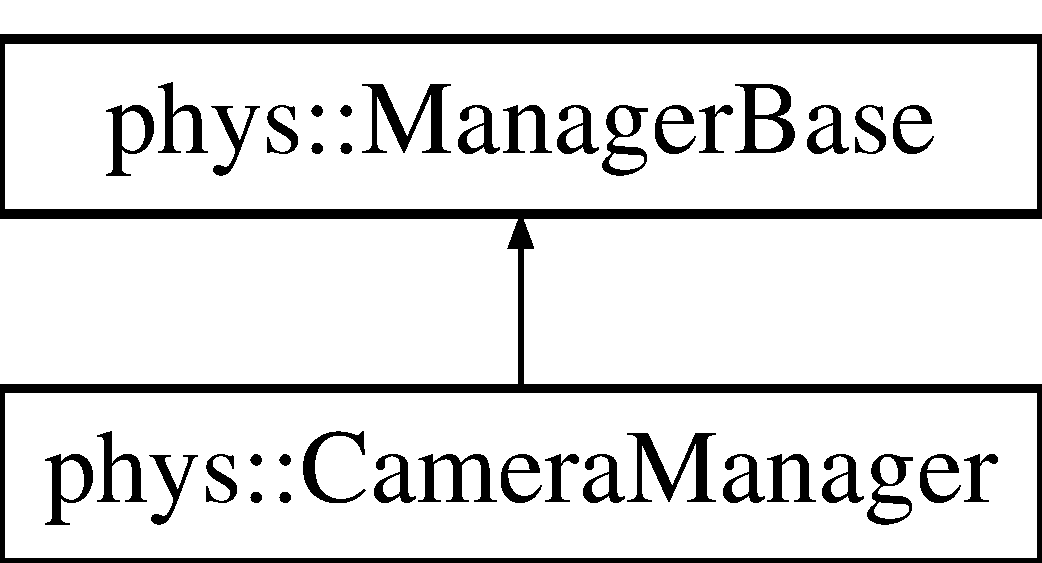
\includegraphics[height=2cm]{d9/d91/classphys_1_1CameraManager}
\end{center}
\end{figure}
\subsection*{Public Member Functions}
\begin{DoxyCompactItemize}
\item 
\hyperlink{classphys_1_1CameraManager_aff47d21e0c80b2b1b44148b0ec7de344}{CameraManager} (Ogre::SceneManager $\ast$SManager)
\begin{DoxyCompactList}\small\item\em Class Constructor. \item\end{DoxyCompactList}\item 
virtual \hyperlink{classphys_1_1CameraManager_a0b0f032477309eb47b0302fd5eef198c}{$\sim$CameraManager} ()
\begin{DoxyCompactList}\small\item\em Class Destructor. \item\end{DoxyCompactList}\item 
\hyperlink{namespacephys_aa03900411993de7fbfec4789bc1d392e}{String} \hyperlink{classphys_1_1CameraManager_ac6ff80c91fa5a2cd21ebd8b78db9add2}{CreateCamera} ()
\begin{DoxyCompactList}\small\item\em Creates a camera. \item\end{DoxyCompactList}\item 
\hyperlink{classphys_1_1Camera}{Camera} $\ast$ \hyperlink{classphys_1_1CameraManager_ae51f79b63b5c34959bc4cfbef34b8f08}{CreateCameraPtr} ()
\begin{DoxyCompactList}\small\item\em Creates a camera and returns a pointer. \item\end{DoxyCompactList}\item 
\hyperlink{namespacephys_aa03900411993de7fbfec4789bc1d392e}{String} \hyperlink{classphys_1_1CameraManager_a9a696ea09f174a69bbc6d0bb179b3de4}{CreateOrbitingNode} (\hyperlink{classphys_1_1Vector3}{Vector3} Target, \hyperlink{classphys_1_1Vector3}{Vector3} RelativeLoc)
\begin{DoxyCompactList}\small\item\em Creates a node that will orbit around a point. \item\end{DoxyCompactList}\item 
\hyperlink{namespacephys_aa03900411993de7fbfec4789bc1d392e}{String} \hyperlink{classphys_1_1CameraManager_ab5f9ca6b053670e69f5812cf573d5972}{CreateStandNode} (\hyperlink{classphys_1_1Vector3}{Vector3} LookAt, \hyperlink{classphys_1_1Vector3}{Vector3} Location)
\begin{DoxyCompactList}\small\item\em Creates a stationary node that will look at a location. \item\end{DoxyCompactList}\item 
void \hyperlink{classphys_1_1CameraManager_a42d91612bbaa00187944290d6bfd44e9}{ClearNodes} ()
\begin{DoxyCompactList}\small\item\em Deletes all nodes created by this manager. \item\end{DoxyCompactList}\item 
void \hyperlink{classphys_1_1CameraManager_a76bebee0820fcfa462412cb112b1b874}{ClearCameras} ()
\begin{DoxyCompactList}\small\item\em Deletes all cameras except for the first camera. \item\end{DoxyCompactList}\item 
void \hyperlink{classphys_1_1CameraManager_a3f1b48057ca2c1cd79f3e61c9fcbe1b4}{SetLocation} (\hyperlink{classphys_1_1Vector3}{Vector3} Location, \hyperlink{namespacephys_aa03900411993de7fbfec4789bc1d392e}{String} Name=\char`\"{}DefaultCamera\char`\"{})
\begin{DoxyCompactList}\small\item\em Sets the location of a camera. \item\end{DoxyCompactList}\item 
void \hyperlink{classphys_1_1CameraManager_aaee96e189230c020d6f7b6fe439e0812}{SetDirection} (\hyperlink{classphys_1_1Vector3}{Vector3} Direction, \hyperlink{namespacephys_aa03900411993de7fbfec4789bc1d392e}{String} Name=\char`\"{}DefaultCamera\char`\"{})
\begin{DoxyCompactList}\small\item\em Sets the Direction for the camera. \item\end{DoxyCompactList}\item 
void \hyperlink{classphys_1_1CameraManager_a9d0fac66fbc2eb4b7247c9661427afb8}{SetOrientation} (\hyperlink{classphys_1_1Quaternion}{Quaternion} Orientation, \hyperlink{namespacephys_aa03900411993de7fbfec4789bc1d392e}{String} Name=\char`\"{}DefaultCamera\char`\"{})
\begin{DoxyCompactList}\small\item\em Sets the orientation of the camera. \item\end{DoxyCompactList}\item 
void \hyperlink{classphys_1_1CameraManager_ad639c275a2bb1c6c05a8800f8e8412c6}{SetNearClipDistance} (\hyperlink{namespacephys_af7eb897198d265b8e868f45240230d5f}{Real} NearDist, \hyperlink{namespacephys_aa03900411993de7fbfec4789bc1d392e}{String} Name=\char`\"{}DefaultCamera\char`\"{})
\begin{DoxyCompactList}\small\item\em Sets the short range clip distance. \item\end{DoxyCompactList}\item 
void \hyperlink{classphys_1_1CameraManager_a809e4e31a9ad42afd620e95508ad78d7}{SetFarClipDistance} (\hyperlink{namespacephys_af7eb897198d265b8e868f45240230d5f}{Real} FarDist, \hyperlink{namespacephys_aa03900411993de7fbfec4789bc1d392e}{String} Name=\char`\"{}DefaultCamera\char`\"{})
\begin{DoxyCompactList}\small\item\em Sets the long range clip distance. \item\end{DoxyCompactList}\item 
void \hyperlink{classphys_1_1CameraManager_af16862039fffd900b9c7acc20527cac8}{SetAspectRatio} (\hyperlink{namespacephys_af7eb897198d265b8e868f45240230d5f}{Real} Ratio, \hyperlink{namespacephys_aa03900411993de7fbfec4789bc1d392e}{String} Name=\char`\"{}DefaultCamera\char`\"{})
\begin{DoxyCompactList}\small\item\em Sets the aspect ratio of the cameras veiw. \item\end{DoxyCompactList}\item 
void \hyperlink{classphys_1_1CameraManager_a885a499a53c3543b6bf429583a2cb54c}{LookAt} (\hyperlink{classphys_1_1Vector3}{Vector3} TargetLoc, \hyperlink{namespacephys_aa03900411993de7fbfec4789bc1d392e}{String} Name=\char`\"{}DefaultCamera\char`\"{})
\begin{DoxyCompactList}\small\item\em Sets the direction the camera faces. \item\end{DoxyCompactList}\item 
void \hyperlink{classphys_1_1CameraManager_ac29a1b3cd34ff2810bee170aa233c77e}{SetFixedYawAxis} (bool UseFixed, \hyperlink{classphys_1_1Vector3}{Vector3} Axis, \hyperlink{namespacephys_aa03900411993de7fbfec4789bc1d392e}{String} Name=\char`\"{}DefaultCamera\char`\"{})
\begin{DoxyCompactList}\small\item\em Sets whether to lock rotation around the Y axis. \item\end{DoxyCompactList}\item 
void \hyperlink{classphys_1_1CameraManager_aa7370f2239e88ab151b72c4171afea07}{SetFixedYawAxis} (bool UseFixed, \hyperlink{namespacephys_aa03900411993de7fbfec4789bc1d392e}{String} Name=\char`\"{}DefaultCamera\char`\"{})
\begin{DoxyCompactList}\small\item\em Sets whether to lock rotation around the Y axis. \item\end{DoxyCompactList}\item 
void \hyperlink{classphys_1_1CameraManager_a43d55c71817096add5dad1552239fc74}{SetAutoTracking} (bool Enabled, \hyperlink{namespacephys_aa03900411993de7fbfec4789bc1d392e}{String} Target, \hyperlink{classphys_1_1Vector3}{Vector3} Offset, \hyperlink{namespacephys_aa03900411993de7fbfec4789bc1d392e}{String} Name=\char`\"{}DefaultCamera\char`\"{})
\begin{DoxyCompactList}\small\item\em Enables or disables auto tracking for the camera. \item\end{DoxyCompactList}\item 
void \hyperlink{classphys_1_1CameraManager_a6edd94b6e8d9f2fa1e0b84554b367933}{SetAutoTracking} (bool Enabled, \hyperlink{namespacephys_aa03900411993de7fbfec4789bc1d392e}{String} Target, \hyperlink{namespacephys_aa03900411993de7fbfec4789bc1d392e}{String} Name=\char`\"{}DefaultCamera\char`\"{})
\begin{DoxyCompactList}\small\item\em Enables or disables auto tracking for the camera. \item\end{DoxyCompactList}\item 
\hyperlink{classphys_1_1Ray}{Ray} \hyperlink{classphys_1_1CameraManager_a1a631eee22a0e45e2e72727d0bcc3560}{GetCameraToViewportRay} (\hyperlink{namespacephys_af7eb897198d265b8e868f45240230d5f}{Real} Screenx, \hyperlink{namespacephys_af7eb897198d265b8e868f45240230d5f}{Real} Screeny, \hyperlink{namespacephys_aa03900411993de7fbfec4789bc1d392e}{String} Name=\char`\"{}DefaultCamera\char`\"{})
\begin{DoxyCompactList}\small\item\em Gets a \hyperlink{classphys_1_1Ray}{Ray} from the camera to the viewport. \item\end{DoxyCompactList}\item 
\hyperlink{namespacephys_aa03900411993de7fbfec4789bc1d392e}{String} \hyperlink{classphys_1_1CameraManager_a52a62fcfbeed45a2f527f626731ddcc1}{GetNodeAttachedToCamera} (\hyperlink{namespacephys_aa03900411993de7fbfec4789bc1d392e}{String} Name=\char`\"{}DefaultCamera\char`\"{})
\begin{DoxyCompactList}\small\item\em Gets the node attached to a camera. \item\end{DoxyCompactList}\item 
\hyperlink{classphys_1_1Vector3}{Vector3} \hyperlink{classphys_1_1CameraManager_af5fcec9bebd90b8e98b0d2f4def97ea1}{GetNodeLocation} (\hyperlink{namespacephys_aa03900411993de7fbfec4789bc1d392e}{String} Name)
\begin{DoxyCompactList}\small\item\em Gets the location of a node. \item\end{DoxyCompactList}\item 
\hyperlink{classphys_1_1Vector3}{Vector3} \hyperlink{classphys_1_1CameraManager_a8557218460fbc94a029f74945fa2517c}{GetCameraRelativeLocation} (\hyperlink{namespacephys_aa03900411993de7fbfec4789bc1d392e}{String} Name=\char`\"{}DefaultCamera\char`\"{})
\begin{DoxyCompactList}\small\item\em Gets the relative location of a camera. \item\end{DoxyCompactList}\item 
\hyperlink{classphys_1_1Vector3}{Vector3} \hyperlink{classphys_1_1CameraManager_a53ef7e8f0a4227a5a35db88fe74772fa}{GetCameraGlobalLocation} (\hyperlink{namespacephys_aa03900411993de7fbfec4789bc1d392e}{String} Name=\char`\"{}DefaultCamera\char`\"{})
\begin{DoxyCompactList}\small\item\em Gets the global location of a camera. \item\end{DoxyCompactList}\item 
void \hyperlink{classphys_1_1CameraManager_aa5a37dbdd45a53bc3dfd4cfa0a94bd42}{ZoomCamera} (\hyperlink{namespacephys_af7eb897198d265b8e868f45240230d5f}{Real} Zoom, \hyperlink{namespacephys_aa03900411993de7fbfec4789bc1d392e}{String} Name=\char`\"{}DefaultCamera\char`\"{})
\begin{DoxyCompactList}\small\item\em Will zoom in or out the camera. \item\end{DoxyCompactList}\item 
void \hyperlink{classphys_1_1CameraManager_a1cfaf4720fa9af7c0f234d6a2f26e179}{ResetZoom} (\hyperlink{namespacephys_aa03900411993de7fbfec4789bc1d392e}{String} Name=\char`\"{}DefaultCamera\char`\"{})
\begin{DoxyCompactList}\small\item\em Resets the zoom level back to the default. \item\end{DoxyCompactList}\item 
void \hyperlink{classphys_1_1CameraManager_a1cde365b6cab80a33ddf7046489f7af9}{AttachCameraToNode} (\hyperlink{namespacephys_aa03900411993de7fbfec4789bc1d392e}{String} NodeName, \hyperlink{namespacephys_aa03900411993de7fbfec4789bc1d392e}{String} CamName=\char`\"{}DefaultCamera\char`\"{})
\begin{DoxyCompactList}\small\item\em Attaches a camera to a node. \item\end{DoxyCompactList}\item 
void \hyperlink{classphys_1_1CameraManager_a5137bdb9dec706fa0fafec665d4f71c8}{DetachCameraFromNode} (\hyperlink{namespacephys_aa03900411993de7fbfec4789bc1d392e}{String} NodeName, \hyperlink{namespacephys_aa03900411993de7fbfec4789bc1d392e}{String} CamName=\char`\"{}DefaultCamera\char`\"{})
\begin{DoxyCompactList}\small\item\em Detaches a camera from a node. \item\end{DoxyCompactList}\item 
void \hyperlink{classphys_1_1CameraManager_a82001f0874a090717ced3fbe78ce795b}{IncrementYOrbit} (\hyperlink{namespacephys_af7eb897198d265b8e868f45240230d5f}{Real} Radian, \hyperlink{namespacephys_aa03900411993de7fbfec4789bc1d392e}{String} Name)
\begin{DoxyCompactList}\small\item\em Increments the orbit by the amount specified. \item\end{DoxyCompactList}\item 
virtual void \hyperlink{classphys_1_1CameraManager_a5e956b61fa341ae576d8d160da518488}{Initialize} ()
\begin{DoxyCompactList}\small\item\em Empty Initializor. \item\end{DoxyCompactList}\item 
virtual \hyperlink{classphys_1_1ManagerBase_aaa6ccddf23892eaccb898529414f80a5}{ManagerTypeName} \hyperlink{classphys_1_1CameraManager_a8412ea634307aa280b615a3cc7c9b739}{GetType} () const 
\begin{DoxyCompactList}\small\item\em This returns the type of this manager. \item\end{DoxyCompactList}\end{DoxyCompactItemize}
\subsection*{Friends}
\begin{DoxyCompactItemize}
\item 
\hypertarget{classphys_1_1CameraManager_a7b4bcdf992c21ae83363f25df05b1d25}{
class {\bfseries World}}
\label{d9/d91/classphys_1_1CameraManager_a7b4bcdf992c21ae83363f25df05b1d25}

\item 
\hypertarget{classphys_1_1CameraManager_ad8bd9afbbd7af19d996da80e9d25890d}{
class {\bfseries Camera}}
\label{d9/d91/classphys_1_1CameraManager_ad8bd9afbbd7af19d996da80e9d25890d}

\end{DoxyCompactItemize}


\subsection{Detailed Description}
This is the manager class for all camera functions. This class contains all the functionality of the use and manipulation of the camera. \par
 All functions that manipulate the camera will default to the default camera, so if you only use one camera you should never have to name the camera you want to use. 

Definition at line 69 of file cameramanager.h.



\subsection{Constructor \& Destructor Documentation}
\hypertarget{classphys_1_1CameraManager_aff47d21e0c80b2b1b44148b0ec7de344}{
\index{phys::CameraManager@{phys::CameraManager}!CameraManager@{CameraManager}}
\index{CameraManager@{CameraManager}!phys::CameraManager@{phys::CameraManager}}
\subsubsection[{CameraManager}]{\setlength{\rightskip}{0pt plus 5cm}phys::CameraManager::CameraManager (Ogre::SceneManager $\ast$ {\em SManager})}}
\label{d9/d91/classphys_1_1CameraManager_aff47d21e0c80b2b1b44148b0ec7de344}


Class Constructor. 

This is the class constructor. This is automatcally called in the World.CreateRenderWindow() function and should never need to be called manually. 
\begin{DoxyParams}{Parameters}
\item[{\em SManager}]A pointer to the Scenemanager where you will be creating/manipulating all the cameras. \end{DoxyParams}


Definition at line 53 of file cameramanager.cpp.

\hypertarget{classphys_1_1CameraManager_a0b0f032477309eb47b0302fd5eef198c}{
\index{phys::CameraManager@{phys::CameraManager}!$\sim$CameraManager@{$\sim$CameraManager}}
\index{$\sim$CameraManager@{$\sim$CameraManager}!phys::CameraManager@{phys::CameraManager}}
\subsubsection[{$\sim$CameraManager}]{\setlength{\rightskip}{0pt plus 5cm}phys::CameraManager::$\sim$CameraManager ()\hspace{0.3cm}{\ttfamily  \mbox{[}virtual\mbox{]}}}}
\label{d9/d91/classphys_1_1CameraManager_a0b0f032477309eb47b0302fd5eef198c}


Class Destructor. 

The calss Destuctor 

Definition at line 61 of file cameramanager.cpp.



\subsection{Member Function Documentation}
\hypertarget{classphys_1_1CameraManager_a1cde365b6cab80a33ddf7046489f7af9}{
\index{phys::CameraManager@{phys::CameraManager}!AttachCameraToNode@{AttachCameraToNode}}
\index{AttachCameraToNode@{AttachCameraToNode}!phys::CameraManager@{phys::CameraManager}}
\subsubsection[{AttachCameraToNode}]{\setlength{\rightskip}{0pt plus 5cm}void phys::CameraManager::AttachCameraToNode ({\bf String} {\em NodeName}, \/  {\bf String} {\em CamName} = {\ttfamily \char`\"{}DefaultCamera\char`\"{}})}}
\label{d9/d91/classphys_1_1CameraManager_a1cde365b6cab80a33ddf7046489f7af9}


Attaches a camera to a node. 

Attaches the specified camera to the specified node. 
\begin{DoxyParams}{Parameters}
\item[{\em NodeName}]The name of the node to attach the camera to. \item[{\em CamName}]The name of the camera to be manipulated. Defaults to the Default camera. \end{DoxyParams}


Definition at line 408 of file cameramanager.cpp.

\hypertarget{classphys_1_1CameraManager_a76bebee0820fcfa462412cb112b1b874}{
\index{phys::CameraManager@{phys::CameraManager}!ClearCameras@{ClearCameras}}
\index{ClearCameras@{ClearCameras}!phys::CameraManager@{phys::CameraManager}}
\subsubsection[{ClearCameras}]{\setlength{\rightskip}{0pt plus 5cm}void phys::CameraManager::ClearCameras ()}}
\label{d9/d91/classphys_1_1CameraManager_a76bebee0820fcfa462412cb112b1b874}


Deletes all cameras except for the first camera. 

This will clear the container of cameras. The default camera is not stored in this container however, so it is spared from this wipe. 

Definition at line 178 of file cameramanager.cpp.

\hypertarget{classphys_1_1CameraManager_a42d91612bbaa00187944290d6bfd44e9}{
\index{phys::CameraManager@{phys::CameraManager}!ClearNodes@{ClearNodes}}
\index{ClearNodes@{ClearNodes}!phys::CameraManager@{phys::CameraManager}}
\subsubsection[{ClearNodes}]{\setlength{\rightskip}{0pt plus 5cm}void phys::CameraManager::ClearNodes ()}}
\label{d9/d91/classphys_1_1CameraManager_a42d91612bbaa00187944290d6bfd44e9}


Deletes all nodes created by this manager. 

This will clear the container of nodes. Including Orbiting nodes, Center nodes, and Stand nodes. 

Definition at line 172 of file cameramanager.cpp.

\hypertarget{classphys_1_1CameraManager_ac6ff80c91fa5a2cd21ebd8b78db9add2}{
\index{phys::CameraManager@{phys::CameraManager}!CreateCamera@{CreateCamera}}
\index{CreateCamera@{CreateCamera}!phys::CameraManager@{phys::CameraManager}}
\subsubsection[{CreateCamera}]{\setlength{\rightskip}{0pt plus 5cm}{\bf String} phys::CameraManager::CreateCamera ()}}
\label{d9/d91/classphys_1_1CameraManager_ac6ff80c91fa5a2cd21ebd8b78db9add2}


Creates a camera. 

This function will create a camera in the scene and return the string that is name of the camera created. The first camera created will always be the Default camera, and is also created just after this class is constructed in the World.CreateRenderWindow() function. 

Definition at line 101 of file cameramanager.cpp.

\hypertarget{classphys_1_1CameraManager_ae51f79b63b5c34959bc4cfbef34b8f08}{
\index{phys::CameraManager@{phys::CameraManager}!CreateCameraPtr@{CreateCameraPtr}}
\index{CreateCameraPtr@{CreateCameraPtr}!phys::CameraManager@{phys::CameraManager}}
\subsubsection[{CreateCameraPtr}]{\setlength{\rightskip}{0pt plus 5cm}{\bf Camera} $\ast$ phys::CameraManager::CreateCameraPtr ()}}
\label{d9/d91/classphys_1_1CameraManager_ae51f79b63b5c34959bc4cfbef34b8f08}


Creates a camera and returns a pointer. 

This function does the same as the other CreateCamera function but will also return a pointer to the camera class instead of a string(being the name of the camera). 

Definition at line 117 of file cameramanager.cpp.

\hypertarget{classphys_1_1CameraManager_a9a696ea09f174a69bbc6d0bb179b3de4}{
\index{phys::CameraManager@{phys::CameraManager}!CreateOrbitingNode@{CreateOrbitingNode}}
\index{CreateOrbitingNode@{CreateOrbitingNode}!phys::CameraManager@{phys::CameraManager}}
\subsubsection[{CreateOrbitingNode}]{\setlength{\rightskip}{0pt plus 5cm}{\bf String} phys::CameraManager::CreateOrbitingNode ({\bf Vector3} {\em Target}, \/  {\bf Vector3} {\em RelativeLoc})}}
\label{d9/d91/classphys_1_1CameraManager_a9a696ea09f174a69bbc6d0bb179b3de4}


Creates a node that will orbit around a point. 

This will create 2 nodes in the scene, the first being the point in the world you want to orbit the second node around. The second being the node that does the orbiting. You can then attach a camera to the orbiting node for some interesting visuals of your scene. 
\begin{DoxyParams}{Parameters}
\item[{\em Target}]The location of the first node which you will be orbiting around. \item[{\em RelativeLoc}]The location of the node that will be in orbit relative to the first node. Assume the first node is at Origin (0,0,0). \end{DoxyParams}


Definition at line 135 of file cameramanager.cpp.

\hypertarget{classphys_1_1CameraManager_ab5f9ca6b053670e69f5812cf573d5972}{
\index{phys::CameraManager@{phys::CameraManager}!CreateStandNode@{CreateStandNode}}
\index{CreateStandNode@{CreateStandNode}!phys::CameraManager@{phys::CameraManager}}
\subsubsection[{CreateStandNode}]{\setlength{\rightskip}{0pt plus 5cm}{\bf String} phys::CameraManager::CreateStandNode ({\bf Vector3} {\em LookAt}, \/  {\bf Vector3} {\em Location})}}
\label{d9/d91/classphys_1_1CameraManager_ab5f9ca6b053670e69f5812cf573d5972}


Creates a stationary node that will look at a location. 

This will create a node that doesn't move, and will look at one location that you specify. This node can then have cameras attached to it. 
\begin{DoxyParams}{Parameters}
\item[{\em LookAt}]The location you want the node to look at. Automatically handles orientation. \item[{\em Location}]The location of the node itself. \end{DoxyParams}


Definition at line 158 of file cameramanager.cpp.

\hypertarget{classphys_1_1CameraManager_a5137bdb9dec706fa0fafec665d4f71c8}{
\index{phys::CameraManager@{phys::CameraManager}!DetachCameraFromNode@{DetachCameraFromNode}}
\index{DetachCameraFromNode@{DetachCameraFromNode}!phys::CameraManager@{phys::CameraManager}}
\subsubsection[{DetachCameraFromNode}]{\setlength{\rightskip}{0pt plus 5cm}void phys::CameraManager::DetachCameraFromNode ({\bf String} {\em NodeName}, \/  {\bf String} {\em CamName} = {\ttfamily \char`\"{}DefaultCamera\char`\"{}})}}
\label{d9/d91/classphys_1_1CameraManager_a5137bdb9dec706fa0fafec665d4f71c8}


Detaches a camera from a node. 

Detaches the specified camera from the specified node. 
\begin{DoxyParams}{Parameters}
\item[{\em NodeName}]The name of the node to detach the camera from. \item[{\em CamName}]The name of the camera to be manipulated. Defaults to the Default camera. \end{DoxyParams}


Definition at line 422 of file cameramanager.cpp.

\hypertarget{classphys_1_1CameraManager_a53ef7e8f0a4227a5a35db88fe74772fa}{
\index{phys::CameraManager@{phys::CameraManager}!GetCameraGlobalLocation@{GetCameraGlobalLocation}}
\index{GetCameraGlobalLocation@{GetCameraGlobalLocation}!phys::CameraManager@{phys::CameraManager}}
\subsubsection[{GetCameraGlobalLocation}]{\setlength{\rightskip}{0pt plus 5cm}{\bf Vector3} phys::CameraManager::GetCameraGlobalLocation ({\bf String} {\em Name} = {\ttfamily \char`\"{}DefaultCamera\char`\"{}})}}
\label{d9/d91/classphys_1_1CameraManager_a53ef7e8f0a4227a5a35db88fe74772fa}


Gets the global location of a camera. 

Gets the real world location of the camera specified. 
\begin{DoxyParams}{Parameters}
\item[{\em Name}]The name of the camera to be manipulated. Defaults to the Default camera. \end{DoxyParams}


Definition at line 364 of file cameramanager.cpp.

\hypertarget{classphys_1_1CameraManager_a8557218460fbc94a029f74945fa2517c}{
\index{phys::CameraManager@{phys::CameraManager}!GetCameraRelativeLocation@{GetCameraRelativeLocation}}
\index{GetCameraRelativeLocation@{GetCameraRelativeLocation}!phys::CameraManager@{phys::CameraManager}}
\subsubsection[{GetCameraRelativeLocation}]{\setlength{\rightskip}{0pt plus 5cm}{\bf Vector3} phys::CameraManager::GetCameraRelativeLocation ({\bf String} {\em Name} = {\ttfamily \char`\"{}DefaultCamera\char`\"{}})}}
\label{d9/d91/classphys_1_1CameraManager_a8557218460fbc94a029f74945fa2517c}


Gets the relative location of a camera. 

Gets the location of the camera, relative to any connected nodes, specified. 
\begin{DoxyParams}{Parameters}
\item[{\em Name}]The name of the camera to be manipulated. Defaults to the Default camera. \end{DoxyParams}


Definition at line 352 of file cameramanager.cpp.

\hypertarget{classphys_1_1CameraManager_a1a631eee22a0e45e2e72727d0bcc3560}{
\index{phys::CameraManager@{phys::CameraManager}!GetCameraToViewportRay@{GetCameraToViewportRay}}
\index{GetCameraToViewportRay@{GetCameraToViewportRay}!phys::CameraManager@{phys::CameraManager}}
\subsubsection[{GetCameraToViewportRay}]{\setlength{\rightskip}{0pt plus 5cm}{\bf Ray} phys::CameraManager::GetCameraToViewportRay ({\bf Real} {\em Screenx}, \/  {\bf Real} {\em Screeny}, \/  {\bf String} {\em Name} = {\ttfamily \char`\"{}DefaultCamera\char`\"{}})}}
\label{d9/d91/classphys_1_1CameraManager_a1a631eee22a0e45e2e72727d0bcc3560}


Gets a \hyperlink{classphys_1_1Ray}{Ray} from the camera to the viewport. 

This will cast a ray from the camera to the viewport and return it. 
\begin{DoxyParams}{Parameters}
\item[{\em Screenx}]A Real representing the relative location on screen, on the x axis(0.0-\/1.0). \item[{\em Screeny}]A Real representing the relative location on screen, on the y axis(0.0-\/1.0). \item[{\em Name}]The name of the camera to be manipulated. Defaults to the Default camera. \end{DoxyParams}


Definition at line 320 of file cameramanager.cpp.

\hypertarget{classphys_1_1CameraManager_a52a62fcfbeed45a2f527f626731ddcc1}{
\index{phys::CameraManager@{phys::CameraManager}!GetNodeAttachedToCamera@{GetNodeAttachedToCamera}}
\index{GetNodeAttachedToCamera@{GetNodeAttachedToCamera}!phys::CameraManager@{phys::CameraManager}}
\subsubsection[{GetNodeAttachedToCamera}]{\setlength{\rightskip}{0pt plus 5cm}{\bf String} phys::CameraManager::GetNodeAttachedToCamera ({\bf String} {\em Name} = {\ttfamily \char`\"{}DefaultCamera\char`\"{}})}}
\label{d9/d91/classphys_1_1CameraManager_a52a62fcfbeed45a2f527f626731ddcc1}


Gets the node attached to a camera. 

This will return a string that is the name of the node the specified camera is attached to if any. 
\begin{DoxyParams}{Parameters}
\item[{\em Name}]The name of the camera to be manipulated. Defaults to the Default camera. \end{DoxyParams}


Definition at line 332 of file cameramanager.cpp.

\hypertarget{classphys_1_1CameraManager_af5fcec9bebd90b8e98b0d2f4def97ea1}{
\index{phys::CameraManager@{phys::CameraManager}!GetNodeLocation@{GetNodeLocation}}
\index{GetNodeLocation@{GetNodeLocation}!phys::CameraManager@{phys::CameraManager}}
\subsubsection[{GetNodeLocation}]{\setlength{\rightskip}{0pt plus 5cm}{\bf Vector3} phys::CameraManager::GetNodeLocation ({\bf String} {\em Name})}}
\label{d9/d91/classphys_1_1CameraManager_af5fcec9bebd90b8e98b0d2f4def97ea1}


Gets the location of a node. 

Gets the location of the node specified. 
\begin{DoxyParams}{Parameters}
\item[{\em Name}]Name of the node to get the location of. \end{DoxyParams}


Definition at line 344 of file cameramanager.cpp.

\hypertarget{classphys_1_1CameraManager_a8412ea634307aa280b615a3cc7c9b739}{
\index{phys::CameraManager@{phys::CameraManager}!GetType@{GetType}}
\index{GetType@{GetType}!phys::CameraManager@{phys::CameraManager}}
\subsubsection[{GetType}]{\setlength{\rightskip}{0pt plus 5cm}{\bf ManagerBase::ManagerTypeName} phys::CameraManager::GetType () const\hspace{0.3cm}{\ttfamily  \mbox{[}virtual\mbox{]}}}}
\label{d9/d91/classphys_1_1CameraManager_a8412ea634307aa280b615a3cc7c9b739}


This returns the type of this manager. 

\begin{DoxyReturn}{Returns}
This returns ManagerTypeName::CameraManager 
\end{DoxyReturn}


Implements \hyperlink{classphys_1_1ManagerBase_aff400b6599db635e24796d8221e9a0e3}{phys::ManagerBase}.



Definition at line 441 of file cameramanager.cpp.

\hypertarget{classphys_1_1CameraManager_a82001f0874a090717ced3fbe78ce795b}{
\index{phys::CameraManager@{phys::CameraManager}!IncrementYOrbit@{IncrementYOrbit}}
\index{IncrementYOrbit@{IncrementYOrbit}!phys::CameraManager@{phys::CameraManager}}
\subsubsection[{IncrementYOrbit}]{\setlength{\rightskip}{0pt plus 5cm}void phys::CameraManager::IncrementYOrbit ({\bf Real} {\em Radian}, \/  {\bf String} {\em Name})}}
\label{d9/d91/classphys_1_1CameraManager_a82001f0874a090717ced3fbe78ce795b}


Increments the orbit by the amount specified. 

Increments the orbit of the specified node by the amount specified. 
\begin{DoxyParams}{Parameters}
\item[{\em Radian}]The amount you wish to increment the orbit in Radians. \item[{\em Name}]The name of the orbiting node you wish to increment the orbit for. \end{DoxyParams}


Definition at line 430 of file cameramanager.cpp.

\hypertarget{classphys_1_1CameraManager_a5e956b61fa341ae576d8d160da518488}{
\index{phys::CameraManager@{phys::CameraManager}!Initialize@{Initialize}}
\index{Initialize@{Initialize}!phys::CameraManager@{phys::CameraManager}}
\subsubsection[{Initialize}]{\setlength{\rightskip}{0pt plus 5cm}void phys::CameraManager::Initialize ()\hspace{0.3cm}{\ttfamily  \mbox{[}virtual\mbox{]}}}}
\label{d9/d91/classphys_1_1CameraManager_a5e956b61fa341ae576d8d160da518488}


Empty Initializor. 

This specific initializor is unneeded, but we implement it for compatibility. It also exists in case a derived class wants to override it for some reason 

Implements \hyperlink{classphys_1_1ManagerBase_a57dd8e54e767427d5bdcc86dc66d73ed}{phys::ManagerBase}.



Definition at line 438 of file cameramanager.cpp.

\hypertarget{classphys_1_1CameraManager_a885a499a53c3543b6bf429583a2cb54c}{
\index{phys::CameraManager@{phys::CameraManager}!LookAt@{LookAt}}
\index{LookAt@{LookAt}!phys::CameraManager@{phys::CameraManager}}
\subsubsection[{LookAt}]{\setlength{\rightskip}{0pt plus 5cm}void phys::CameraManager::LookAt ({\bf Vector3} {\em TargetLoc}, \/  {\bf String} {\em Name} = {\ttfamily \char`\"{}DefaultCamera\char`\"{}})}}
\label{d9/d91/classphys_1_1CameraManager_a885a499a53c3543b6bf429583a2cb54c}


Sets the direction the camera faces. 

Sets the direction the camera faces. Will also take orientation into account. 
\begin{DoxyParams}{Parameters}
\item[{\em TargetLoc}]The location in the game world to look at. \item[{\em Name}]The name of the camera to be manipulated. Defaults to the Default camera. \end{DoxyParams}


Definition at line 256 of file cameramanager.cpp.

\hypertarget{classphys_1_1CameraManager_a1cfaf4720fa9af7c0f234d6a2f26e179}{
\index{phys::CameraManager@{phys::CameraManager}!ResetZoom@{ResetZoom}}
\index{ResetZoom@{ResetZoom}!phys::CameraManager@{phys::CameraManager}}
\subsubsection[{ResetZoom}]{\setlength{\rightskip}{0pt plus 5cm}void phys::CameraManager::ResetZoom ({\bf String} {\em Name} = {\ttfamily \char`\"{}DefaultCamera\char`\"{}})}}
\label{d9/d91/classphys_1_1CameraManager_a1cfaf4720fa9af7c0f234d6a2f26e179}


Resets the zoom level back to the default. 

This function will return the zoom level back to normal. Note this function will only work if the camera is attached to a node. 
\begin{DoxyParams}{Parameters}
\item[{\em Name}]The name of the camera to be manipulated. Defaults to the Default camera. \end{DoxyParams}


Definition at line 389 of file cameramanager.cpp.

\hypertarget{classphys_1_1CameraManager_af16862039fffd900b9c7acc20527cac8}{
\index{phys::CameraManager@{phys::CameraManager}!SetAspectRatio@{SetAspectRatio}}
\index{SetAspectRatio@{SetAspectRatio}!phys::CameraManager@{phys::CameraManager}}
\subsubsection[{SetAspectRatio}]{\setlength{\rightskip}{0pt plus 5cm}void phys::CameraManager::SetAspectRatio ({\bf Real} {\em Ratio}, \/  {\bf String} {\em Name} = {\ttfamily \char`\"{}DefaultCamera\char`\"{}})}}
\label{d9/d91/classphys_1_1CameraManager_af16862039fffd900b9c7acc20527cac8}


Sets the aspect ratio of the cameras veiw. 

This function will set the aspect ratio between the width and height of the cameras viewing area. 
\begin{DoxyParams}{Parameters}
\item[{\em Ratio}]A Real that represents the aspect ratio, where Ratio = width / height. \item[{\em Name}]The name of the camera to be manipulated. Defaults to the Default camera. \end{DoxyParams}


Definition at line 244 of file cameramanager.cpp.

\hypertarget{classphys_1_1CameraManager_a6edd94b6e8d9f2fa1e0b84554b367933}{
\index{phys::CameraManager@{phys::CameraManager}!SetAutoTracking@{SetAutoTracking}}
\index{SetAutoTracking@{SetAutoTracking}!phys::CameraManager@{phys::CameraManager}}
\subsubsection[{SetAutoTracking}]{\setlength{\rightskip}{0pt plus 5cm}void phys::CameraManager::SetAutoTracking (bool {\em Enabled}, \/  {\bf String} {\em Target}, \/  {\bf String} {\em Name} = {\ttfamily \char`\"{}DefaultCamera\char`\"{}})}}
\label{d9/d91/classphys_1_1CameraManager_a6edd94b6e8d9f2fa1e0b84554b367933}


Enables or disables auto tracking for the camera. 

This function can enable auto tracking of a given node you have created. 
\begin{DoxyParams}{Parameters}
\item[{\em Enabled}]Bool value to enable or disable auto tracking for this camera. \item[{\em Target}]Name of the node to be tracked. \item[{\em Name}]The name of the camera to be manipulated. Defaults to the Default camera. \end{DoxyParams}


Definition at line 306 of file cameramanager.cpp.

\hypertarget{classphys_1_1CameraManager_a43d55c71817096add5dad1552239fc74}{
\index{phys::CameraManager@{phys::CameraManager}!SetAutoTracking@{SetAutoTracking}}
\index{SetAutoTracking@{SetAutoTracking}!phys::CameraManager@{phys::CameraManager}}
\subsubsection[{SetAutoTracking}]{\setlength{\rightskip}{0pt plus 5cm}void phys::CameraManager::SetAutoTracking (bool {\em Enabled}, \/  {\bf String} {\em Target}, \/  {\bf Vector3} {\em Offset}, \/  {\bf String} {\em Name} = {\ttfamily \char`\"{}DefaultCamera\char`\"{}})}}
\label{d9/d91/classphys_1_1CameraManager_a43d55c71817096add5dad1552239fc74}


Enables or disables auto tracking for the camera. 

This function can enable auto tracking of a given node you have created. 
\begin{DoxyParams}{Parameters}
\item[{\em Enabled}]Bool value to enable or disable auto tracking for this camera. \item[{\em Target}]Name of the node to be tracked. \item[{\em Offset}]The offset of where the camera is to look from the target. I.E. Always 5 units ahead, etc.. \item[{\em Name}]The name of the camera to be manipulated. Defaults to the Default camera. \end{DoxyParams}


Definition at line 292 of file cameramanager.cpp.

\hypertarget{classphys_1_1CameraManager_aaee96e189230c020d6f7b6fe439e0812}{
\index{phys::CameraManager@{phys::CameraManager}!SetDirection@{SetDirection}}
\index{SetDirection@{SetDirection}!phys::CameraManager@{phys::CameraManager}}
\subsubsection[{SetDirection}]{\setlength{\rightskip}{0pt plus 5cm}void phys::CameraManager::SetDirection ({\bf Vector3} {\em Direction}, \/  {\bf String} {\em Name} = {\ttfamily \char`\"{}DefaultCamera\char`\"{}})}}
\label{d9/d91/classphys_1_1CameraManager_aaee96e189230c020d6f7b6fe439e0812}


Sets the Direction for the camera. 

Sets which axis the camera will look down for rendering. 
\begin{DoxyParams}{Parameters}
\item[{\em Direction}]The vector3 representing the axis to be used. \item[{\em Name}]The name of the camera to be manipulated. Defaults to the Default camera. \end{DoxyParams}


Definition at line 196 of file cameramanager.cpp.

\hypertarget{classphys_1_1CameraManager_a809e4e31a9ad42afd620e95508ad78d7}{
\index{phys::CameraManager@{phys::CameraManager}!SetFarClipDistance@{SetFarClipDistance}}
\index{SetFarClipDistance@{SetFarClipDistance}!phys::CameraManager@{phys::CameraManager}}
\subsubsection[{SetFarClipDistance}]{\setlength{\rightskip}{0pt plus 5cm}void phys::CameraManager::SetFarClipDistance ({\bf Real} {\em FarDist}, \/  {\bf String} {\em Name} = {\ttfamily \char`\"{}DefaultCamera\char`\"{}})}}
\label{d9/d91/classphys_1_1CameraManager_a809e4e31a9ad42afd620e95508ad78d7}


Sets the long range clip distance. 

Sets the distance at which objects are considered too far to render. 
\begin{DoxyParams}{Parameters}
\item[{\em FarDist}]A Real representing the distance. Note: This number directly corolates to the dimentions you provide in the constructor for the physgame. You should understand your games scale before setting this number. \item[{\em Name}]The name of the camera to be manipulated. Defaults to the Default camera. \end{DoxyParams}


Definition at line 232 of file cameramanager.cpp.

\hypertarget{classphys_1_1CameraManager_aa7370f2239e88ab151b72c4171afea07}{
\index{phys::CameraManager@{phys::CameraManager}!SetFixedYawAxis@{SetFixedYawAxis}}
\index{SetFixedYawAxis@{SetFixedYawAxis}!phys::CameraManager@{phys::CameraManager}}
\subsubsection[{SetFixedYawAxis}]{\setlength{\rightskip}{0pt plus 5cm}void phys::CameraManager::SetFixedYawAxis (bool {\em UseFixed}, \/  {\bf String} {\em Name} = {\ttfamily \char`\"{}DefaultCamera\char`\"{}})}}
\label{d9/d91/classphys_1_1CameraManager_aa7370f2239e88ab151b72c4171afea07}


Sets whether to lock rotation around the Y axis. 

This function will lock rotations around the Y axis. This function is automatically called on by the camera constructor. 
\begin{DoxyParams}{Parameters}
\item[{\em UseFixed}]Enable or disable the locking of the axis. \item[{\em Name}]The name of the camera to be manipulated. Defaults to the Default camera. \end{DoxyParams}


Definition at line 280 of file cameramanager.cpp.

\hypertarget{classphys_1_1CameraManager_ac29a1b3cd34ff2810bee170aa233c77e}{
\index{phys::CameraManager@{phys::CameraManager}!SetFixedYawAxis@{SetFixedYawAxis}}
\index{SetFixedYawAxis@{SetFixedYawAxis}!phys::CameraManager@{phys::CameraManager}}
\subsubsection[{SetFixedYawAxis}]{\setlength{\rightskip}{0pt plus 5cm}void phys::CameraManager::SetFixedYawAxis (bool {\em UseFixed}, \/  {\bf Vector3} {\em Axis}, \/  {\bf String} {\em Name} = {\ttfamily \char`\"{}DefaultCamera\char`\"{}})}}
\label{d9/d91/classphys_1_1CameraManager_ac29a1b3cd34ff2810bee170aa233c77e}


Sets whether to lock rotation around the Y axis. 

This function will lock rotations around the Y axis (or another axis if you specify). This function is automatically called on by the camera constructor. 
\begin{DoxyParams}{Parameters}
\item[{\em UseFixed}]Enable or disable the locking of the axis. \item[{\em Axis}]The axis to lock, defaults to the Y axis. \item[{\em Name}]The name of the camera to be manipulated. Defaults to the Default camera. \end{DoxyParams}


Definition at line 268 of file cameramanager.cpp.

\hypertarget{classphys_1_1CameraManager_a3f1b48057ca2c1cd79f3e61c9fcbe1b4}{
\index{phys::CameraManager@{phys::CameraManager}!SetLocation@{SetLocation}}
\index{SetLocation@{SetLocation}!phys::CameraManager@{phys::CameraManager}}
\subsubsection[{SetLocation}]{\setlength{\rightskip}{0pt plus 5cm}void phys::CameraManager::SetLocation ({\bf Vector3} {\em Location}, \/  {\bf String} {\em Name} = {\ttfamily \char`\"{}DefaultCamera\char`\"{}})}}
\label{d9/d91/classphys_1_1CameraManager_a3f1b48057ca2c1cd79f3e61c9fcbe1b4}


Sets the location of a camera. 

Sets the location of the specified camera. 
\begin{DoxyParams}{Parameters}
\item[{\em Location}]The new location for the camera. \item[{\em Name}]The name of the camera to be manipulated. Defaults to the Default camera. \end{DoxyParams}


Definition at line 184 of file cameramanager.cpp.

\hypertarget{classphys_1_1CameraManager_ad639c275a2bb1c6c05a8800f8e8412c6}{
\index{phys::CameraManager@{phys::CameraManager}!SetNearClipDistance@{SetNearClipDistance}}
\index{SetNearClipDistance@{SetNearClipDistance}!phys::CameraManager@{phys::CameraManager}}
\subsubsection[{SetNearClipDistance}]{\setlength{\rightskip}{0pt plus 5cm}void phys::CameraManager::SetNearClipDistance ({\bf Real} {\em NearDist}, \/  {\bf String} {\em Name} = {\ttfamily \char`\"{}DefaultCamera\char`\"{}})}}
\label{d9/d91/classphys_1_1CameraManager_ad639c275a2bb1c6c05a8800f8e8412c6}


Sets the short range clip distance. 

Sets the distance at which objects are considered too close to render. 
\begin{DoxyParams}{Parameters}
\item[{\em NearDist}]A Real representing the distance. Note: This number directly corolates to the dimentions you provide in the constructor for the physgame. You should understand your games scale before setting this number. \item[{\em Name}]The name of the camera to be manipulated. Defaults to the Default camera. \end{DoxyParams}


Definition at line 220 of file cameramanager.cpp.

\hypertarget{classphys_1_1CameraManager_a9d0fac66fbc2eb4b7247c9661427afb8}{
\index{phys::CameraManager@{phys::CameraManager}!SetOrientation@{SetOrientation}}
\index{SetOrientation@{SetOrientation}!phys::CameraManager@{phys::CameraManager}}
\subsubsection[{SetOrientation}]{\setlength{\rightskip}{0pt plus 5cm}void phys::CameraManager::SetOrientation ({\bf Quaternion} {\em Orientation}, \/  {\bf String} {\em Name} = {\ttfamily \char`\"{}DefaultCamera\char`\"{}})}}
\label{d9/d91/classphys_1_1CameraManager_a9d0fac66fbc2eb4b7247c9661427afb8}


Sets the orientation of the camera. 

This function will set the orientation of the specified camera via a quaternion. 
\begin{DoxyParams}{Parameters}
\item[{\em Orientation}]The quaternion representing the new orientation. \item[{\em Name}]The name of the camera to be manipulated. Defaults to the Default camera. \end{DoxyParams}


Definition at line 208 of file cameramanager.cpp.

\hypertarget{classphys_1_1CameraManager_aa5a37dbdd45a53bc3dfd4cfa0a94bd42}{
\index{phys::CameraManager@{phys::CameraManager}!ZoomCamera@{ZoomCamera}}
\index{ZoomCamera@{ZoomCamera}!phys::CameraManager@{phys::CameraManager}}
\subsubsection[{ZoomCamera}]{\setlength{\rightskip}{0pt plus 5cm}void phys::CameraManager::ZoomCamera ({\bf Real} {\em Zoom}, \/  {\bf String} {\em Name} = {\ttfamily \char`\"{}DefaultCamera\char`\"{}})}}
\label{d9/d91/classphys_1_1CameraManager_aa5a37dbdd45a53bc3dfd4cfa0a94bd42}


Will zoom in or out the camera. 

This function will zoom in the camera by the amount specified. 
\begin{DoxyParams}{Parameters}
\item[{\em Zoom}]A Real of how much to zoom in by. Note: This number directly corolates to the dimentions you provide in the constructor for the physgame. You should understand your games scale before setting this number. \item[{\em Name}]The name of the camera to be manipulated. Defaults to the Default camera. \end{DoxyParams}


Definition at line 376 of file cameramanager.cpp.



The documentation for this class was generated from the following files:\begin{DoxyCompactItemize}
\item 
cameramanager.h\item 
cameramanager.cpp\end{DoxyCompactItemize}

\hypertarget{classphys_1_1UI_1_1Caption}{
\subsection{phys::UI::Caption Class Reference}
\label{d4/dfe/classphys_1_1UI_1_1Caption}\index{phys::UI::Caption@{phys::UI::Caption}}
}


This class is a helper class, specifically for use with text.  




{\ttfamily \#include $<$uicaption.h$>$}

\subsubsection*{Public Member Functions}
\begin{DoxyCompactItemize}
\item 
\hyperlink{classphys_1_1UI_1_1Caption_a8e643db77a6f9b18147cf01cf3bd9238}{Caption} (\hyperlink{namespacephys_a5ce5049f8b4bf88d6413c47b504ebb31}{ConstString} \&name, const \hyperlink{classphys_1_1Vector2}{Vector2} Position, const \hyperlink{classphys_1_1Vector2}{Vector2} Size, const \hyperlink{namespacephys_a460f6bc24c8dd347b05e0366ae34f34a}{Whole} Glyph, \hyperlink{namespacephys_aa03900411993de7fbfec4789bc1d392e}{String} Text, \hyperlink{classphys_1_1UILayer}{UILayer} $\ast$Layer)
\begin{DoxyCompactList}\small\item\em Internal constructor. \item\end{DoxyCompactList}\item 
\hypertarget{classphys_1_1UI_1_1Caption_a5443ce0c7c7dc4b4f1c56b124e092a98}{
virtual \hyperlink{classphys_1_1UI_1_1Caption_a5443ce0c7c7dc4b4f1c56b124e092a98}{$\sim$Caption} ()}
\label{d4/dfe/classphys_1_1UI_1_1Caption_a5443ce0c7c7dc4b4f1c56b124e092a98}

\begin{DoxyCompactList}\small\item\em Class destructor. \item\end{DoxyCompactList}\item 
virtual void \hyperlink{classphys_1_1UI_1_1Caption_afce46e42eb3ab522c29d5c13a5691065}{SetVisible} (bool Visible)
\begin{DoxyCompactList}\small\item\em Sets the visibility of this caption. \item\end{DoxyCompactList}\item 
virtual bool \hyperlink{classphys_1_1UI_1_1Caption_a965d162160c26a2f9a2a16b88aa8f05d}{IsVisible} ()
\begin{DoxyCompactList}\small\item\em Gets the visibility of this caption. \item\end{DoxyCompactList}\item 
\hypertarget{classphys_1_1UI_1_1Caption_a9801eaaadf70f7373b410995b255936e}{
virtual void \hyperlink{classphys_1_1UI_1_1Caption_a9801eaaadf70f7373b410995b255936e}{Show} ()}
\label{d4/dfe/classphys_1_1UI_1_1Caption_a9801eaaadf70f7373b410995b255936e}

\begin{DoxyCompactList}\small\item\em Forces this caption to be shown. \item\end{DoxyCompactList}\item 
\hypertarget{classphys_1_1UI_1_1Caption_a12e772b19e723334747fcf2ca009965c}{
virtual void \hyperlink{classphys_1_1UI_1_1Caption_a12e772b19e723334747fcf2ca009965c}{Hide} ()}
\label{d4/dfe/classphys_1_1UI_1_1Caption_a12e772b19e723334747fcf2ca009965c}

\begin{DoxyCompactList}\small\item\em Forces this caption to hide. \item\end{DoxyCompactList}\item 
virtual bool \hyperlink{classphys_1_1UI_1_1Caption_a3dc84a08ea80de8d75e9614decbad605}{CheckMouseHover} ()
\begin{DoxyCompactList}\small\item\em Determines whether the mouse is over this caption. \item\end{DoxyCompactList}\item 
virtual bool \hyperlink{classphys_1_1UI_1_1Caption_afdb8c018e33bc28c77291ea797c042c0}{GetMouseHover} ()
\begin{DoxyCompactList}\small\item\em Gets the stored value of whether or not the mouse is over the caption. \item\end{DoxyCompactList}\item 
virtual \hyperlink{namespacephys_a5ce5049f8b4bf88d6413c47b504ebb31}{ConstString} \& \hyperlink{classphys_1_1UI_1_1Caption_ac189115176b58b77b32b5b61fe8fec1b}{GetName} ()
\begin{DoxyCompactList}\small\item\em Gets the name of this caption. \item\end{DoxyCompactList}\item 
virtual void \hyperlink{classphys_1_1UI_1_1Caption_a4592228fd6874958e6767b9d461ac2ce}{SetText} (\hyperlink{namespacephys_a5ce5049f8b4bf88d6413c47b504ebb31}{ConstString} \&Text)
\begin{DoxyCompactList}\small\item\em Sets the text displayed within the caption. \item\end{DoxyCompactList}\item 
virtual \hyperlink{namespacephys_aa03900411993de7fbfec4789bc1d392e}{String} \hyperlink{classphys_1_1UI_1_1Caption_ad35be48f6f9df9ca9d9a2e3d0cb99c78}{GetText} ()
\begin{DoxyCompactList}\small\item\em Gets the text displayed within the caption. \item\end{DoxyCompactList}\item 
virtual void \hyperlink{classphys_1_1UI_1_1Caption_a3dad9c0c70e461734166937f6961a459}{SetTextScale} (\hyperlink{namespacephys_af7eb897198d265b8e868f45240230d5f}{Real} Scale)
\begin{DoxyCompactList}\small\item\em Sets the scaling to be applied to the text being rendered. \item\end{DoxyCompactList}\item 
virtual \hyperlink{namespacephys_af7eb897198d265b8e868f45240230d5f}{Real} \hyperlink{classphys_1_1UI_1_1Caption_a6c916aef18864826feca84a6b8ddf619}{GetTextScale} ()
\begin{DoxyCompactList}\small\item\em Gets the scaling currently being applied to the rendered text. \item\end{DoxyCompactList}\item 
virtual void \hyperlink{classphys_1_1UI_1_1Caption_a48e02a811a03a7542ee9bdcc4303a264}{SetTextColour} (const \hyperlink{classphys_1_1ColourValue}{ColourValue} \&TextColour)
\begin{DoxyCompactList}\small\item\em Sets the colour for the text in this caption. \item\end{DoxyCompactList}\item 
virtual \hyperlink{classphys_1_1ColourValue}{ColourValue} \hyperlink{classphys_1_1UI_1_1Caption_a32bb578e6e92986839e1cd49edfe9422}{GetTextColour} ()
\begin{DoxyCompactList}\small\item\em Gets the colour for the text in this caption. \item\end{DoxyCompactList}\item 
virtual void \hyperlink{classphys_1_1UI_1_1Caption_a854b4f5d5a18c4e5f0cebeb17cf2ece4}{SetGlyphIndex} (const \hyperlink{namespacephys_a460f6bc24c8dd347b05e0366ae34f34a}{Whole} GlyphIndex)
\begin{DoxyCompactList}\small\item\em Sets the glyph index to be used with this caption. \item\end{DoxyCompactList}\item 
virtual \hyperlink{namespacephys_a460f6bc24c8dd347b05e0366ae34f34a}{Whole} \hyperlink{classphys_1_1UI_1_1Caption_a4181591a3186ec4d1f87946891a0ef26}{GetGlyphIndex} ()
\begin{DoxyCompactList}\small\item\em Gets the glyph index in use by this caption. \item\end{DoxyCompactList}\item 
virtual void \hyperlink{classphys_1_1UI_1_1Caption_a55c748adf8f23689c71c38fab284b567}{SetCursorOffset} (const \hyperlink{namespacephys_a460f6bc24c8dd347b05e0366ae34f34a}{Whole} Offset)
\begin{DoxyCompactList}\small\item\em Sets the number of pixels text should be offset from the side when rendering. \item\end{DoxyCompactList}\item 
virtual \hyperlink{namespacephys_a460f6bc24c8dd347b05e0366ae34f34a}{Whole} \hyperlink{classphys_1_1UI_1_1Caption_a381133922b882500ae0bf503acb4c6a4}{GetCursorOffset} ()
\begin{DoxyCompactList}\small\item\em Gets the number of pixels text should be offset from the side when rendering. \item\end{DoxyCompactList}\item 
virtual void \hyperlink{classphys_1_1UI_1_1Caption_a33ec6c09671474529b0f33f0f1cd51ad}{SetBackgroundColour} (const \hyperlink{classphys_1_1ColourValue}{ColourValue} \&Colour)
\begin{DoxyCompactList}\small\item\em Sets the background colour of the caption. \item\end{DoxyCompactList}\item 
virtual void \hyperlink{classphys_1_1UI_1_1Caption_a98422dc633dfb68ea87d0f54fda25f48}{SetBackgroundSprite} (const \hyperlink{namespacephys_aa03900411993de7fbfec4789bc1d392e}{String} \&Name)
\begin{DoxyCompactList}\small\item\em Sets the background image(if provided in the atlas) of the caption. \item\end{DoxyCompactList}\item 
virtual void \hyperlink{classphys_1_1UI_1_1Caption_a1b7d2736ee545f518c33f0cd99a4ef0a}{HorizontallyAlign} (UI::TextHorizontalAlign Align)
\begin{DoxyCompactList}\small\item\em Aligns the text of the caption. \item\end{DoxyCompactList}\item 
virtual void \hyperlink{classphys_1_1UI_1_1Caption_adb3936d7eea2137e60943825acf4a5d0}{VerticallyAlign} (UI::TextVerticalAlign Align)
\begin{DoxyCompactList}\small\item\em Aligns the text of the caption. \item\end{DoxyCompactList}\item 
virtual void \hyperlink{classphys_1_1UI_1_1Caption_a3a0e4e927afe9c8fb7fd4f3771fc3bd0}{SetPosition} (const \hyperlink{classphys_1_1Vector2}{Vector2} Position)
\begin{DoxyCompactList}\small\item\em Sets the relative top left position of this caption. \item\end{DoxyCompactList}\item 
virtual \hyperlink{classphys_1_1Vector2}{Vector2} \hyperlink{classphys_1_1UI_1_1Caption_a3096383b16f81c3b4894afd61110ffa0}{GetPosition} ()
\begin{DoxyCompactList}\small\item\em Gets the relative top left position of this caption. \item\end{DoxyCompactList}\item 
virtual void \hyperlink{classphys_1_1UI_1_1Caption_a49b9972c95d710a9496d9cc2ca486890}{SetActualPosition} (const \hyperlink{classphys_1_1Vector2}{Vector2} Position)
\begin{DoxyCompactList}\small\item\em Sets the top left position of this caption in pixels. \item\end{DoxyCompactList}\item 
virtual \hyperlink{classphys_1_1Vector2}{Vector2} \hyperlink{classphys_1_1UI_1_1Caption_aae3e6728a26111e12b081992d6d04e1a}{GetActualPosition} ()
\begin{DoxyCompactList}\small\item\em Gets the top left position of this caption in pixels. \item\end{DoxyCompactList}\item 
virtual void \hyperlink{classphys_1_1UI_1_1Caption_a9551a0efc894dd97cead9db69f018f5d}{SetSize} (const \hyperlink{classphys_1_1Vector2}{Vector2} Size)
\begin{DoxyCompactList}\small\item\em Sets the relative size of this caption. \item\end{DoxyCompactList}\item 
virtual \hyperlink{classphys_1_1Vector2}{Vector2} \hyperlink{classphys_1_1UI_1_1Caption_a1da2e0e9ce0d904595f53a10244fcaf4}{GetSize} ()
\begin{DoxyCompactList}\small\item\em Gets the relative size of this caption. \item\end{DoxyCompactList}\item 
virtual void \hyperlink{classphys_1_1UI_1_1Caption_ad92716cc1c3ad3544aab5e892ae24225}{SetActualSize} (const \hyperlink{classphys_1_1Vector2}{Vector2} Size)
\begin{DoxyCompactList}\small\item\em Sets the size of this caption in pixels. \item\end{DoxyCompactList}\item 
virtual \hyperlink{classphys_1_1Vector2}{Vector2} \hyperlink{classphys_1_1UI_1_1Caption_aa80a4328d76458a6e869c485bea48b98}{GetActualSize} ()
\begin{DoxyCompactList}\small\item\em Gets the size of this caption in pixels. \item\end{DoxyCompactList}\item 
virtual void \hyperlink{classphys_1_1UI_1_1Caption_a27e71736c847ff6e50be7191e3db5225}{SetRenderPriority} (UI::RenderPriority Priority)
\begin{DoxyCompactList}\small\item\em Sets the priority this caption should be rendered with. \item\end{DoxyCompactList}\item 
virtual UI::RenderPriority \hyperlink{classphys_1_1UI_1_1Caption_ada0bf1e830f8f672adbc3263e7095896}{GetRenderPriority} ()
\begin{DoxyCompactList}\small\item\em Gets the priority this caption should be rendered with. \item\end{DoxyCompactList}\end{DoxyCompactItemize}
\subsubsection*{Protected Attributes}
\begin{DoxyCompactItemize}
\item 
\hypertarget{classphys_1_1UI_1_1Caption_a7a93d509acea460f79c40cb0306709d4}{
Gorilla::Caption $\ast$ {\bfseries GorillaCaption}}
\label{d4/dfe/classphys_1_1UI_1_1Caption_a7a93d509acea460f79c40cb0306709d4}

\item 
\hypertarget{classphys_1_1UI_1_1Caption_a784ae5ce5d499f1905e6e7a121e26ac0}{
Gorilla::Rectangle $\ast$ {\bfseries GorillaRectangle}}
\label{d4/dfe/classphys_1_1UI_1_1Caption_a784ae5ce5d499f1905e6e7a121e26ac0}

\item 
\hypertarget{classphys_1_1UI_1_1Caption_a10f1d8cde30267671f082947d8fbdcab}{
\hyperlink{classphys_1_1UILayer}{UILayer} $\ast$ {\bfseries Parent}}
\label{d4/dfe/classphys_1_1UI_1_1Caption_a10f1d8cde30267671f082947d8fbdcab}

\item 
\hypertarget{classphys_1_1UI_1_1Caption_a1102b88d8e70c89191f15826aac2afa5}{
\hyperlink{classphys_1_1UIManager}{UIManager} $\ast$ {\bfseries Manager}}
\label{d4/dfe/classphys_1_1UI_1_1Caption_a1102b88d8e70c89191f15826aac2afa5}

\item 
\hypertarget{classphys_1_1UI_1_1Caption_a466a606964575ebbd1af6a91ed3b9375}{
\hyperlink{namespacephys_a460f6bc24c8dd347b05e0366ae34f34a}{Whole} {\bfseries Glyphs}}
\label{d4/dfe/classphys_1_1UI_1_1Caption_a466a606964575ebbd1af6a91ed3b9375}

\item 
\hypertarget{classphys_1_1UI_1_1Caption_a9923417253f29965257d7fb9f707542e}{
bool {\bfseries MouseHover}}
\label{d4/dfe/classphys_1_1UI_1_1Caption_a9923417253f29965257d7fb9f707542e}

\item 
\hypertarget{classphys_1_1UI_1_1Caption_a63061f6c9799bea406eba1060ec9daa4}{
\hyperlink{classphys_1_1Vector2}{Vector2} {\bfseries RelPosition}}
\label{d4/dfe/classphys_1_1UI_1_1Caption_a63061f6c9799bea406eba1060ec9daa4}

\item 
\hypertarget{classphys_1_1UI_1_1Caption_acd511c5bc0d19986a1869d5d5e4f9094}{
\hyperlink{classphys_1_1Vector2}{Vector2} {\bfseries RelSize}}
\label{d4/dfe/classphys_1_1UI_1_1Caption_acd511c5bc0d19986a1869d5d5e4f9094}

\item 
\hypertarget{classphys_1_1UI_1_1Caption_a6d5f0c79c720695e3f4e009e590a8827}{
\hyperlink{namespacephys_aa03900411993de7fbfec4789bc1d392e}{String} {\bfseries Name}}
\label{d4/dfe/classphys_1_1UI_1_1Caption_a6d5f0c79c720695e3f4e009e590a8827}

\end{DoxyCompactItemize}


\subsubsection{Detailed Description}
This class is a helper class, specifically for use with text. Unlike a button, this class cannot be interacted with by clicking. It is important to understand what you want your space to do when selecting the class to use. \par
 \par
 Markup Texts and Captions are similar in that they both display text messages that can be altered readily, the primary difference between the two is that Captions are meant for small simple messages with background functionality built in, where as Markup Texts have no background functionality, but they use a light markup language to accomplish special effects with the text. 

Definition at line 73 of file uicaption.h.



\subsubsection{Constructor \& Destructor Documentation}
\hypertarget{classphys_1_1UI_1_1Caption_a8e643db77a6f9b18147cf01cf3bd9238}{
\index{phys::UI::Caption@{phys::UI::Caption}!Caption@{Caption}}
\index{Caption@{Caption}!phys::UI::Caption@{phys::UI::Caption}}
\paragraph[{Caption}]{\setlength{\rightskip}{0pt plus 5cm}phys::UI::Caption::Caption (
\begin{DoxyParamCaption}
\item[{{\bf ConstString} \&}]{ name, }
\item[{const {\bf Vector2}}]{ Position, }
\item[{const {\bf Vector2}}]{ Size, }
\item[{const {\bf Whole}}]{ Glyph, }
\item[{{\bf String}}]{ Text, }
\item[{{\bf UILayer} $\ast$}]{ Layer}
\end{DoxyParamCaption}
)}\hfill}
\label{d4/dfe/classphys_1_1UI_1_1Caption_a8e643db77a6f9b18147cf01cf3bd9238}


Internal constructor. 


\begin{DoxyParams}{Parameters}
\item[{\em Name}]The name of this caption. \item[{\em Position}]The top left position of the caption. \item[{\em Size}]The size of the \hyperlink{classphys_1_1UI_1_1Button}{Button}. \item[{\em Glyph}]One of the glyphs specified in your gorilla file. Must be valid. \item[{\em Text}]Any text you want printed on the caption. \item[{\em Layer}]Pointer to the layer that created this caption. \end{DoxyParams}


Definition at line 57 of file uicaption.cpp.



\subsubsection{Member Function Documentation}
\hypertarget{classphys_1_1UI_1_1Caption_a3dc84a08ea80de8d75e9614decbad605}{
\index{phys::UI::Caption@{phys::UI::Caption}!CheckMouseHover@{CheckMouseHover}}
\index{CheckMouseHover@{CheckMouseHover}!phys::UI::Caption@{phys::UI::Caption}}
\paragraph[{CheckMouseHover}]{\setlength{\rightskip}{0pt plus 5cm}bool phys::UI::Caption::CheckMouseHover (
\begin{DoxyParamCaption}
{}
\end{DoxyParamCaption}
)\hspace{0.3cm}{\ttfamily  \mbox{[}virtual\mbox{]}}}\hfill}
\label{d4/dfe/classphys_1_1UI_1_1Caption_a3dc84a08ea80de8d75e9614decbad605}


Determines whether the mouse is over this caption. 

\begin{DoxyReturn}{Returns}
Returns a bool indicating whether the mouse is over this caption. 
\end{DoxyReturn}


Definition at line 104 of file uicaption.cpp.

\hypertarget{classphys_1_1UI_1_1Caption_aae3e6728a26111e12b081992d6d04e1a}{
\index{phys::UI::Caption@{phys::UI::Caption}!GetActualPosition@{GetActualPosition}}
\index{GetActualPosition@{GetActualPosition}!phys::UI::Caption@{phys::UI::Caption}}
\paragraph[{GetActualPosition}]{\setlength{\rightskip}{0pt plus 5cm}{\bf Vector2} phys::UI::Caption::GetActualPosition (
\begin{DoxyParamCaption}
{}
\end{DoxyParamCaption}
)\hspace{0.3cm}{\ttfamily  \mbox{[}virtual\mbox{]}}}\hfill}
\label{d4/dfe/classphys_1_1UI_1_1Caption_aae3e6728a26111e12b081992d6d04e1a}


Gets the top left position of this caption in pixels. 

\begin{DoxyReturn}{Returns}
Returns a \hyperlink{classphys_1_1Vector2}{Vector2} representing the location of this caption. 
\end{DoxyReturn}


Definition at line 255 of file uicaption.cpp.

\hypertarget{classphys_1_1UI_1_1Caption_aa80a4328d76458a6e869c485bea48b98}{
\index{phys::UI::Caption@{phys::UI::Caption}!GetActualSize@{GetActualSize}}
\index{GetActualSize@{GetActualSize}!phys::UI::Caption@{phys::UI::Caption}}
\paragraph[{GetActualSize}]{\setlength{\rightskip}{0pt plus 5cm}{\bf Vector2} phys::UI::Caption::GetActualSize (
\begin{DoxyParamCaption}
{}
\end{DoxyParamCaption}
)\hspace{0.3cm}{\ttfamily  \mbox{[}virtual\mbox{]}}}\hfill}
\label{d4/dfe/classphys_1_1UI_1_1Caption_aa80a4328d76458a6e869c485bea48b98}


Gets the size of this caption in pixels. 

\begin{DoxyReturn}{Returns}
Returns a vector2 representing the size of this caption. 
\end{DoxyReturn}


Definition at line 284 of file uicaption.cpp.

\hypertarget{classphys_1_1UI_1_1Caption_a381133922b882500ae0bf503acb4c6a4}{
\index{phys::UI::Caption@{phys::UI::Caption}!GetCursorOffset@{GetCursorOffset}}
\index{GetCursorOffset@{GetCursorOffset}!phys::UI::Caption@{phys::UI::Caption}}
\paragraph[{GetCursorOffset}]{\setlength{\rightskip}{0pt plus 5cm}{\bf Whole} phys::UI::Caption::GetCursorOffset (
\begin{DoxyParamCaption}
{}
\end{DoxyParamCaption}
)\hspace{0.3cm}{\ttfamily  \mbox{[}virtual\mbox{]}}}\hfill}
\label{d4/dfe/classphys_1_1UI_1_1Caption_a381133922b882500ae0bf503acb4c6a4}


Gets the number of pixels text should be offset from the side when rendering. 

\begin{DoxyReturn}{Returns}
Returns a Whole representing the number of pixels text is currently being offset from the side. 
\end{DoxyReturn}


Definition at line 175 of file uicaption.cpp.

\hypertarget{classphys_1_1UI_1_1Caption_a4181591a3186ec4d1f87946891a0ef26}{
\index{phys::UI::Caption@{phys::UI::Caption}!GetGlyphIndex@{GetGlyphIndex}}
\index{GetGlyphIndex@{GetGlyphIndex}!phys::UI::Caption@{phys::UI::Caption}}
\paragraph[{GetGlyphIndex}]{\setlength{\rightskip}{0pt plus 5cm}{\bf Whole} phys::UI::Caption::GetGlyphIndex (
\begin{DoxyParamCaption}
{}
\end{DoxyParamCaption}
)\hspace{0.3cm}{\ttfamily  \mbox{[}virtual\mbox{]}}}\hfill}
\label{d4/dfe/classphys_1_1UI_1_1Caption_a4181591a3186ec4d1f87946891a0ef26}


Gets the glyph index in use by this caption. 

The glyph index is defined in your gorilla file. 
\begin{DoxyParams}{Parameters}
\item[{\em Returns}]a Whole representing the index of the glyph in use by this caption.. \end{DoxyParams}


Definition at line 165 of file uicaption.cpp.

\hypertarget{classphys_1_1UI_1_1Caption_afdb8c018e33bc28c77291ea797c042c0}{
\index{phys::UI::Caption@{phys::UI::Caption}!GetMouseHover@{GetMouseHover}}
\index{GetMouseHover@{GetMouseHover}!phys::UI::Caption@{phys::UI::Caption}}
\paragraph[{GetMouseHover}]{\setlength{\rightskip}{0pt plus 5cm}bool phys::UI::Caption::GetMouseHover (
\begin{DoxyParamCaption}
{}
\end{DoxyParamCaption}
)\hspace{0.3cm}{\ttfamily  \mbox{[}virtual\mbox{]}}}\hfill}
\label{d4/dfe/classphys_1_1UI_1_1Caption_afdb8c018e33bc28c77291ea797c042c0}


Gets the stored value of whether or not the mouse is over the caption. 

This function does not perform any checks. If you want to do a manual check, call \hyperlink{classphys_1_1UI_1_1Caption_a3dc84a08ea80de8d75e9614decbad605}{CheckMouseHover()}. \begin{DoxyReturn}{Returns}
Returns the stored value of whether or not the mouse is over the caption. 
\end{DoxyReturn}


Definition at line 118 of file uicaption.cpp.

\hypertarget{classphys_1_1UI_1_1Caption_ac189115176b58b77b32b5b61fe8fec1b}{
\index{phys::UI::Caption@{phys::UI::Caption}!GetName@{GetName}}
\index{GetName@{GetName}!phys::UI::Caption@{phys::UI::Caption}}
\paragraph[{GetName}]{\setlength{\rightskip}{0pt plus 5cm}{\bf ConstString} \& phys::UI::Caption::GetName (
\begin{DoxyParamCaption}
{}
\end{DoxyParamCaption}
)\hspace{0.3cm}{\ttfamily  \mbox{[}virtual\mbox{]}}}\hfill}
\label{d4/dfe/classphys_1_1UI_1_1Caption_ac189115176b58b77b32b5b61fe8fec1b}


Gets the name of this caption. 

\begin{DoxyReturn}{Returns}
Returns a string containing the name of this caption. 
\end{DoxyReturn}


Definition at line 123 of file uicaption.cpp.

\hypertarget{classphys_1_1UI_1_1Caption_a3096383b16f81c3b4894afd61110ffa0}{
\index{phys::UI::Caption@{phys::UI::Caption}!GetPosition@{GetPosition}}
\index{GetPosition@{GetPosition}!phys::UI::Caption@{phys::UI::Caption}}
\paragraph[{GetPosition}]{\setlength{\rightskip}{0pt plus 5cm}{\bf Vector2} phys::UI::Caption::GetPosition (
\begin{DoxyParamCaption}
{}
\end{DoxyParamCaption}
)\hspace{0.3cm}{\ttfamily  \mbox{[}virtual\mbox{]}}}\hfill}
\label{d4/dfe/classphys_1_1UI_1_1Caption_a3096383b16f81c3b4894afd61110ffa0}


Gets the relative top left position of this caption. 

\begin{DoxyReturn}{Returns}
Returns a \hyperlink{classphys_1_1Vector2}{Vector2} representing the location of this caption. 
\end{DoxyReturn}


Definition at line 242 of file uicaption.cpp.

\hypertarget{classphys_1_1UI_1_1Caption_ada0bf1e830f8f672adbc3263e7095896}{
\index{phys::UI::Caption@{phys::UI::Caption}!GetRenderPriority@{GetRenderPriority}}
\index{GetRenderPriority@{GetRenderPriority}!phys::UI::Caption@{phys::UI::Caption}}
\paragraph[{GetRenderPriority}]{\setlength{\rightskip}{0pt plus 5cm}UI::RenderPriority phys::UI::Caption::GetRenderPriority (
\begin{DoxyParamCaption}
{}
\end{DoxyParamCaption}
)\hspace{0.3cm}{\ttfamily  \mbox{[}virtual\mbox{]}}}\hfill}
\label{d4/dfe/classphys_1_1UI_1_1Caption_ada0bf1e830f8f672adbc3263e7095896}


Gets the priority this caption should be rendered with. 

\begin{DoxyReturn}{Returns}
Returns an enum value representing this caption's priority level. 
\end{DoxyReturn}


Definition at line 311 of file uicaption.cpp.

\hypertarget{classphys_1_1UI_1_1Caption_a1da2e0e9ce0d904595f53a10244fcaf4}{
\index{phys::UI::Caption@{phys::UI::Caption}!GetSize@{GetSize}}
\index{GetSize@{GetSize}!phys::UI::Caption@{phys::UI::Caption}}
\paragraph[{GetSize}]{\setlength{\rightskip}{0pt plus 5cm}{\bf Vector2} phys::UI::Caption::GetSize (
\begin{DoxyParamCaption}
{}
\end{DoxyParamCaption}
)\hspace{0.3cm}{\ttfamily  \mbox{[}virtual\mbox{]}}}\hfill}
\label{d4/dfe/classphys_1_1UI_1_1Caption_a1da2e0e9ce0d904595f53a10244fcaf4}


Gets the relative size of this caption. 

\begin{DoxyReturn}{Returns}
Returns a vector2 representing the size of this caption. 
\end{DoxyReturn}


Definition at line 271 of file uicaption.cpp.

\hypertarget{classphys_1_1UI_1_1Caption_ad35be48f6f9df9ca9d9a2e3d0cb99c78}{
\index{phys::UI::Caption@{phys::UI::Caption}!GetText@{GetText}}
\index{GetText@{GetText}!phys::UI::Caption@{phys::UI::Caption}}
\paragraph[{GetText}]{\setlength{\rightskip}{0pt plus 5cm}{\bf String} phys::UI::Caption::GetText (
\begin{DoxyParamCaption}
{}
\end{DoxyParamCaption}
)\hspace{0.3cm}{\ttfamily  \mbox{[}virtual\mbox{]}}}\hfill}
\label{d4/dfe/classphys_1_1UI_1_1Caption_ad35be48f6f9df9ca9d9a2e3d0cb99c78}


Gets the text displayed within the caption. 

\begin{DoxyReturn}{Returns}
Returns the text being displayed. 
\end{DoxyReturn}


Definition at line 133 of file uicaption.cpp.

\hypertarget{classphys_1_1UI_1_1Caption_a32bb578e6e92986839e1cd49edfe9422}{
\index{phys::UI::Caption@{phys::UI::Caption}!GetTextColour@{GetTextColour}}
\index{GetTextColour@{GetTextColour}!phys::UI::Caption@{phys::UI::Caption}}
\paragraph[{GetTextColour}]{\setlength{\rightskip}{0pt plus 5cm}{\bf ColourValue} phys::UI::Caption::GetTextColour (
\begin{DoxyParamCaption}
{}
\end{DoxyParamCaption}
)\hspace{0.3cm}{\ttfamily  \mbox{[}virtual\mbox{]}}}\hfill}
\label{d4/dfe/classphys_1_1UI_1_1Caption_a32bb578e6e92986839e1cd49edfe9422}


Gets the colour for the text in this caption. 

\begin{DoxyReturn}{Returns}
Returns a colourvalue representing the currently set colour of the text in this caption. 
\end{DoxyReturn}


Definition at line 153 of file uicaption.cpp.

\hypertarget{classphys_1_1UI_1_1Caption_a6c916aef18864826feca84a6b8ddf619}{
\index{phys::UI::Caption@{phys::UI::Caption}!GetTextScale@{GetTextScale}}
\index{GetTextScale@{GetTextScale}!phys::UI::Caption@{phys::UI::Caption}}
\paragraph[{GetTextScale}]{\setlength{\rightskip}{0pt plus 5cm}{\bf Real} phys::UI::Caption::GetTextScale (
\begin{DoxyParamCaption}
{}
\end{DoxyParamCaption}
)\hspace{0.3cm}{\ttfamily  \mbox{[}virtual\mbox{]}}}\hfill}
\label{d4/dfe/classphys_1_1UI_1_1Caption_a6c916aef18864826feca84a6b8ddf619}


Gets the scaling currently being applied to the rendered text. 

\begin{DoxyReturn}{Returns}
Returns a Real value representing the scale applied to the text in this caption. $<$1.0 means smaller, $>$1.0 means larger. 
\end{DoxyReturn}


Definition at line 143 of file uicaption.cpp.

\hypertarget{classphys_1_1UI_1_1Caption_a1b7d2736ee545f518c33f0cd99a4ef0a}{
\index{phys::UI::Caption@{phys::UI::Caption}!HorizontallyAlign@{HorizontallyAlign}}
\index{HorizontallyAlign@{HorizontallyAlign}!phys::UI::Caption@{phys::UI::Caption}}
\paragraph[{HorizontallyAlign}]{\setlength{\rightskip}{0pt plus 5cm}void phys::UI::Caption::HorizontallyAlign (
\begin{DoxyParamCaption}
\item[{UI::TextHorizontalAlign}]{ Align}
\end{DoxyParamCaption}
)\hspace{0.3cm}{\ttfamily  \mbox{[}virtual\mbox{]}}}\hfill}
\label{d4/dfe/classphys_1_1UI_1_1Caption_a1b7d2736ee545f518c33f0cd99a4ef0a}


Aligns the text of the caption. 

Default value for this is UI::Txt\_\-Middle. 
\begin{DoxyParams}{Parameters}
\item[{\em Align}]The enum value representing the horizontal alignment to be set. \end{DoxyParams}


Definition at line 192 of file uicaption.cpp.

\hypertarget{classphys_1_1UI_1_1Caption_a965d162160c26a2f9a2a16b88aa8f05d}{
\index{phys::UI::Caption@{phys::UI::Caption}!IsVisible@{IsVisible}}
\index{IsVisible@{IsVisible}!phys::UI::Caption@{phys::UI::Caption}}
\paragraph[{IsVisible}]{\setlength{\rightskip}{0pt plus 5cm}bool phys::UI::Caption::IsVisible (
\begin{DoxyParamCaption}
{}
\end{DoxyParamCaption}
)\hspace{0.3cm}{\ttfamily  \mbox{[}virtual\mbox{]}}}\hfill}
\label{d4/dfe/classphys_1_1UI_1_1Caption_a965d162160c26a2f9a2a16b88aa8f05d}


Gets the visibility of this caption. 

\begin{DoxyReturn}{Returns}
Returns a bool representing the visibility of this caption. 
\end{DoxyReturn}


Definition at line 87 of file uicaption.cpp.

\hypertarget{classphys_1_1UI_1_1Caption_a49b9972c95d710a9496d9cc2ca486890}{
\index{phys::UI::Caption@{phys::UI::Caption}!SetActualPosition@{SetActualPosition}}
\index{SetActualPosition@{SetActualPosition}!phys::UI::Caption@{phys::UI::Caption}}
\paragraph[{SetActualPosition}]{\setlength{\rightskip}{0pt plus 5cm}void phys::UI::Caption::SetActualPosition (
\begin{DoxyParamCaption}
\item[{const {\bf Vector2}}]{ Position}
\end{DoxyParamCaption}
)\hspace{0.3cm}{\ttfamily  \mbox{[}virtual\mbox{]}}}\hfill}
\label{d4/dfe/classphys_1_1UI_1_1Caption_a49b9972c95d710a9496d9cc2ca486890}


Sets the top left position of this caption in pixels. 


\begin{DoxyParams}{Parameters}
\item[{\em Position}]A \hyperlink{classphys_1_1Vector2}{Vector2} representing the location of this caption. \end{DoxyParams}


Definition at line 247 of file uicaption.cpp.

\hypertarget{classphys_1_1UI_1_1Caption_ad92716cc1c3ad3544aab5e892ae24225}{
\index{phys::UI::Caption@{phys::UI::Caption}!SetActualSize@{SetActualSize}}
\index{SetActualSize@{SetActualSize}!phys::UI::Caption@{phys::UI::Caption}}
\paragraph[{SetActualSize}]{\setlength{\rightskip}{0pt plus 5cm}void phys::UI::Caption::SetActualSize (
\begin{DoxyParamCaption}
\item[{const {\bf Vector2}}]{ Size}
\end{DoxyParamCaption}
)\hspace{0.3cm}{\ttfamily  \mbox{[}virtual\mbox{]}}}\hfill}
\label{d4/dfe/classphys_1_1UI_1_1Caption_ad92716cc1c3ad3544aab5e892ae24225}


Sets the size of this caption in pixels. 


\begin{DoxyParams}{Parameters}
\item[{\em Size}]A vector2 representing the size of this caption. \end{DoxyParams}


Definition at line 276 of file uicaption.cpp.

\hypertarget{classphys_1_1UI_1_1Caption_a33ec6c09671474529b0f33f0f1cd51ad}{
\index{phys::UI::Caption@{phys::UI::Caption}!SetBackgroundColour@{SetBackgroundColour}}
\index{SetBackgroundColour@{SetBackgroundColour}!phys::UI::Caption@{phys::UI::Caption}}
\paragraph[{SetBackgroundColour}]{\setlength{\rightskip}{0pt plus 5cm}void phys::UI::Caption::SetBackgroundColour (
\begin{DoxyParamCaption}
\item[{const {\bf ColourValue} \&}]{ Colour}
\end{DoxyParamCaption}
)\hspace{0.3cm}{\ttfamily  \mbox{[}virtual\mbox{]}}}\hfill}
\label{d4/dfe/classphys_1_1UI_1_1Caption_a33ec6c09671474529b0f33f0f1cd51ad}


Sets the background colour of the caption. 


\begin{DoxyParams}{Parameters}
\item[{\em Colour}]A colour value representing the colour to be set. \end{DoxyParams}


Definition at line 180 of file uicaption.cpp.

\hypertarget{classphys_1_1UI_1_1Caption_a98422dc633dfb68ea87d0f54fda25f48}{
\index{phys::UI::Caption@{phys::UI::Caption}!SetBackgroundSprite@{SetBackgroundSprite}}
\index{SetBackgroundSprite@{SetBackgroundSprite}!phys::UI::Caption@{phys::UI::Caption}}
\paragraph[{SetBackgroundSprite}]{\setlength{\rightskip}{0pt plus 5cm}void phys::UI::Caption::SetBackgroundSprite (
\begin{DoxyParamCaption}
\item[{const {\bf String} \&}]{ Name}
\end{DoxyParamCaption}
)\hspace{0.3cm}{\ttfamily  \mbox{[}virtual\mbox{]}}}\hfill}
\label{d4/dfe/classphys_1_1UI_1_1Caption_a98422dc633dfb68ea87d0f54fda25f48}


Sets the background image(if provided in the atlas) of the caption. 


\begin{DoxyParams}{Parameters}
\item[{\em Name}]The name of the sprite to set as the background. \end{DoxyParams}


Definition at line 185 of file uicaption.cpp.

\hypertarget{classphys_1_1UI_1_1Caption_a55c748adf8f23689c71c38fab284b567}{
\index{phys::UI::Caption@{phys::UI::Caption}!SetCursorOffset@{SetCursorOffset}}
\index{SetCursorOffset@{SetCursorOffset}!phys::UI::Caption@{phys::UI::Caption}}
\paragraph[{SetCursorOffset}]{\setlength{\rightskip}{0pt plus 5cm}void phys::UI::Caption::SetCursorOffset (
\begin{DoxyParamCaption}
\item[{const {\bf Whole}}]{ Offset}
\end{DoxyParamCaption}
)\hspace{0.3cm}{\ttfamily  \mbox{[}virtual\mbox{]}}}\hfill}
\label{d4/dfe/classphys_1_1UI_1_1Caption_a55c748adf8f23689c71c38fab284b567}


Sets the number of pixels text should be offset from the side when rendering. 

This doesn't apply when text is being rendered with a Middle alignment. 
\begin{DoxyParams}{Parameters}
\item[{\em Offset}]The number of pixels from the side text should be offset. \end{DoxyParams}


Definition at line 170 of file uicaption.cpp.

\hypertarget{classphys_1_1UI_1_1Caption_a854b4f5d5a18c4e5f0cebeb17cf2ece4}{
\index{phys::UI::Caption@{phys::UI::Caption}!SetGlyphIndex@{SetGlyphIndex}}
\index{SetGlyphIndex@{SetGlyphIndex}!phys::UI::Caption@{phys::UI::Caption}}
\paragraph[{SetGlyphIndex}]{\setlength{\rightskip}{0pt plus 5cm}void phys::UI::Caption::SetGlyphIndex (
\begin{DoxyParamCaption}
\item[{const {\bf Whole}}]{ GlyphIndex}
\end{DoxyParamCaption}
)\hspace{0.3cm}{\ttfamily  \mbox{[}virtual\mbox{]}}}\hfill}
\label{d4/dfe/classphys_1_1UI_1_1Caption_a854b4f5d5a18c4e5f0cebeb17cf2ece4}


Sets the glyph index to be used with this caption. 

The glyph index is defined in your gorilla file. 
\begin{DoxyParams}{Parameters}
\item[{\em GlyphIndex}]The index of the glyph to use with this caption. \end{DoxyParams}


Definition at line 159 of file uicaption.cpp.

\hypertarget{classphys_1_1UI_1_1Caption_a3a0e4e927afe9c8fb7fd4f3771fc3bd0}{
\index{phys::UI::Caption@{phys::UI::Caption}!SetPosition@{SetPosition}}
\index{SetPosition@{SetPosition}!phys::UI::Caption@{phys::UI::Caption}}
\paragraph[{SetPosition}]{\setlength{\rightskip}{0pt plus 5cm}void phys::UI::Caption::SetPosition (
\begin{DoxyParamCaption}
\item[{const {\bf Vector2}}]{ Position}
\end{DoxyParamCaption}
)\hspace{0.3cm}{\ttfamily  \mbox{[}virtual\mbox{]}}}\hfill}
\label{d4/dfe/classphys_1_1UI_1_1Caption_a3a0e4e927afe9c8fb7fd4f3771fc3bd0}


Sets the relative top left position of this caption. 


\begin{DoxyParams}{Parameters}
\item[{\em Position}]A \hyperlink{classphys_1_1Vector2}{Vector2} representing the location of this caption. \end{DoxyParams}


Definition at line 232 of file uicaption.cpp.

\hypertarget{classphys_1_1UI_1_1Caption_a27e71736c847ff6e50be7191e3db5225}{
\index{phys::UI::Caption@{phys::UI::Caption}!SetRenderPriority@{SetRenderPriority}}
\index{SetRenderPriority@{SetRenderPriority}!phys::UI::Caption@{phys::UI::Caption}}
\paragraph[{SetRenderPriority}]{\setlength{\rightskip}{0pt plus 5cm}void phys::UI::Caption::SetRenderPriority (
\begin{DoxyParamCaption}
\item[{UI::RenderPriority}]{ Priority}
\end{DoxyParamCaption}
)\hspace{0.3cm}{\ttfamily  \mbox{[}virtual\mbox{]}}}\hfill}
\label{d4/dfe/classphys_1_1UI_1_1Caption_a27e71736c847ff6e50be7191e3db5225}


Sets the priority this caption should be rendered with. 

The default value for this is Medium. 
\begin{DoxyParams}{Parameters}
\item[{\em Priority}]The priority level to be used when rendering this caption. \end{DoxyParams}


Definition at line 290 of file uicaption.cpp.

\hypertarget{classphys_1_1UI_1_1Caption_a9551a0efc894dd97cead9db69f018f5d}{
\index{phys::UI::Caption@{phys::UI::Caption}!SetSize@{SetSize}}
\index{SetSize@{SetSize}!phys::UI::Caption@{phys::UI::Caption}}
\paragraph[{SetSize}]{\setlength{\rightskip}{0pt plus 5cm}void phys::UI::Caption::SetSize (
\begin{DoxyParamCaption}
\item[{const {\bf Vector2}}]{ Size}
\end{DoxyParamCaption}
)\hspace{0.3cm}{\ttfamily  \mbox{[}virtual\mbox{]}}}\hfill}
\label{d4/dfe/classphys_1_1UI_1_1Caption_a9551a0efc894dd97cead9db69f018f5d}


Sets the relative size of this caption. 


\begin{DoxyParams}{Parameters}
\item[{\em Size}]A vector2 representing the size of this caption. \end{DoxyParams}


Definition at line 261 of file uicaption.cpp.

\hypertarget{classphys_1_1UI_1_1Caption_a4592228fd6874958e6767b9d461ac2ce}{
\index{phys::UI::Caption@{phys::UI::Caption}!SetText@{SetText}}
\index{SetText@{SetText}!phys::UI::Caption@{phys::UI::Caption}}
\paragraph[{SetText}]{\setlength{\rightskip}{0pt plus 5cm}void phys::UI::Caption::SetText (
\begin{DoxyParamCaption}
\item[{{\bf ConstString} \&}]{ Text}
\end{DoxyParamCaption}
)\hspace{0.3cm}{\ttfamily  \mbox{[}virtual\mbox{]}}}\hfill}
\label{d4/dfe/classphys_1_1UI_1_1Caption_a4592228fd6874958e6767b9d461ac2ce}


Sets the text displayed within the caption. 


\begin{DoxyParams}{Parameters}
\item[{\em Text}]The text to be displayed. \end{DoxyParams}


Definition at line 128 of file uicaption.cpp.

\hypertarget{classphys_1_1UI_1_1Caption_a48e02a811a03a7542ee9bdcc4303a264}{
\index{phys::UI::Caption@{phys::UI::Caption}!SetTextColour@{SetTextColour}}
\index{SetTextColour@{SetTextColour}!phys::UI::Caption@{phys::UI::Caption}}
\paragraph[{SetTextColour}]{\setlength{\rightskip}{0pt plus 5cm}void phys::UI::Caption::SetTextColour (
\begin{DoxyParamCaption}
\item[{const {\bf ColourValue} \&}]{ TextColour}
\end{DoxyParamCaption}
)\hspace{0.3cm}{\ttfamily  \mbox{[}virtual\mbox{]}}}\hfill}
\label{d4/dfe/classphys_1_1UI_1_1Caption_a48e02a811a03a7542ee9bdcc4303a264}


Sets the colour for the text in this caption. 


\begin{DoxyParams}{Parameters}
\item[{\em TextColour}]A colourvalue representing the desired colour. \end{DoxyParams}


Definition at line 148 of file uicaption.cpp.

\hypertarget{classphys_1_1UI_1_1Caption_a3dad9c0c70e461734166937f6961a459}{
\index{phys::UI::Caption@{phys::UI::Caption}!SetTextScale@{SetTextScale}}
\index{SetTextScale@{SetTextScale}!phys::UI::Caption@{phys::UI::Caption}}
\paragraph[{SetTextScale}]{\setlength{\rightskip}{0pt plus 5cm}void phys::UI::Caption::SetTextScale (
\begin{DoxyParamCaption}
\item[{{\bf Real}}]{ Scale}
\end{DoxyParamCaption}
)\hspace{0.3cm}{\ttfamily  \mbox{[}virtual\mbox{]}}}\hfill}
\label{d4/dfe/classphys_1_1UI_1_1Caption_a3dad9c0c70e461734166937f6961a459}


Sets the scaling to be applied to the text being rendered. 


\begin{DoxyParams}{Parameters}
\item[{\em Scale}]A Real value representing the scale to be applied. $<$1.0 means smaller, $>$1.0 means larger. \end{DoxyParams}


Definition at line 138 of file uicaption.cpp.

\hypertarget{classphys_1_1UI_1_1Caption_afce46e42eb3ab522c29d5c13a5691065}{
\index{phys::UI::Caption@{phys::UI::Caption}!SetVisible@{SetVisible}}
\index{SetVisible@{SetVisible}!phys::UI::Caption@{phys::UI::Caption}}
\paragraph[{SetVisible}]{\setlength{\rightskip}{0pt plus 5cm}void phys::UI::Caption::SetVisible (
\begin{DoxyParamCaption}
\item[{bool}]{ Visible}
\end{DoxyParamCaption}
)\hspace{0.3cm}{\ttfamily  \mbox{[}virtual\mbox{]}}}\hfill}
\label{d4/dfe/classphys_1_1UI_1_1Caption_afce46e42eb3ab522c29d5c13a5691065}


Sets the visibility of this caption. 


\begin{DoxyParams}{Parameters}
\item[{\em Visible}]Bool determining whether or not this caption should be visible. \end{DoxyParams}


Definition at line 81 of file uicaption.cpp.

\hypertarget{classphys_1_1UI_1_1Caption_adb3936d7eea2137e60943825acf4a5d0}{
\index{phys::UI::Caption@{phys::UI::Caption}!VerticallyAlign@{VerticallyAlign}}
\index{VerticallyAlign@{VerticallyAlign}!phys::UI::Caption@{phys::UI::Caption}}
\paragraph[{VerticallyAlign}]{\setlength{\rightskip}{0pt plus 5cm}void phys::UI::Caption::VerticallyAlign (
\begin{DoxyParamCaption}
\item[{UI::TextVerticalAlign}]{ Align}
\end{DoxyParamCaption}
)\hspace{0.3cm}{\ttfamily  \mbox{[}virtual\mbox{]}}}\hfill}
\label{d4/dfe/classphys_1_1UI_1_1Caption_adb3936d7eea2137e60943825acf4a5d0}


Aligns the text of the caption. 

Default value for this is UI::Txt\_\-Center. 
\begin{DoxyParams}{Parameters}
\item[{\em Align}]The enum value representing the vertical alignment to be set. \end{DoxyParams}


Definition at line 212 of file uicaption.cpp.



The documentation for this class was generated from the following files:\begin{DoxyCompactItemize}
\item 
uicaption.h\item 
uicaption.cpp\end{DoxyCompactItemize}

\hypertarget{classphys_1_1UI_1_1CheckBox}{
\subsection{phys::UI::CheckBox Class Reference}
\label{dd/d10/classphys_1_1UI_1_1CheckBox}\index{phys::UI::CheckBox@{phys::UI::CheckBox}}
}


This is a simple widget for storing a bool value.  




{\ttfamily \#include $<$uicheckbox.h$>$}

Inheritance diagram for phys::UI::CheckBox:\begin{figure}[H]
\begin{center}
\leavevmode
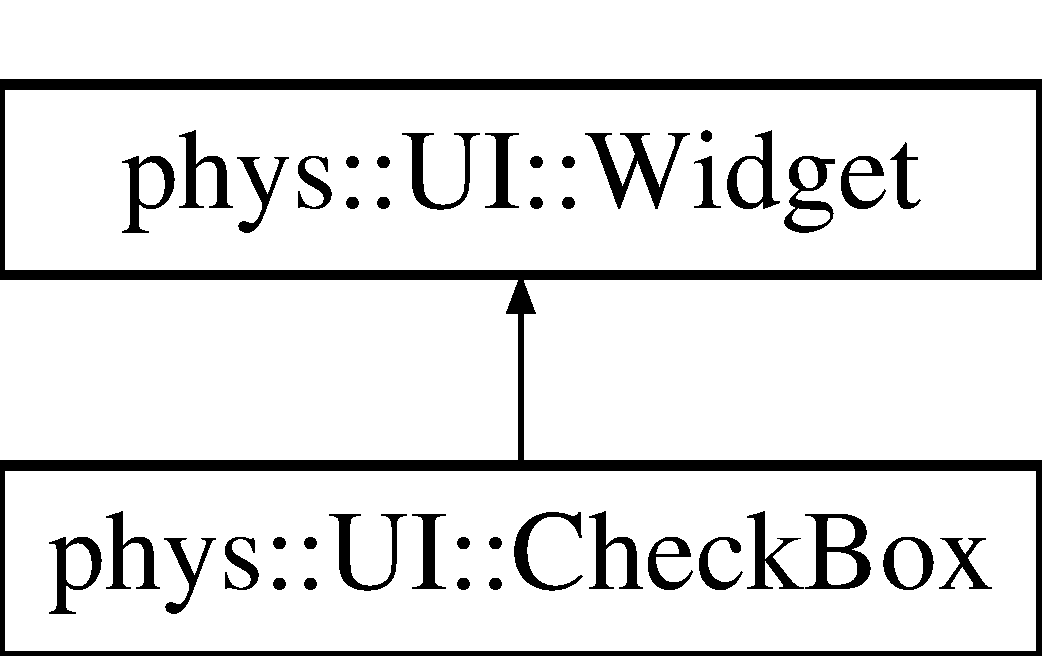
\includegraphics[height=2.000000cm]{dd/d10/classphys_1_1UI_1_1CheckBox}
\end{center}
\end{figure}
\subsubsection*{Public Member Functions}
\begin{DoxyCompactItemize}
\item 
\hyperlink{classphys_1_1UI_1_1CheckBox_aa6952188a51cb452f2a34c5c2cc134ff}{CheckBox} (\hyperlink{namespacephys_a5ce5049f8b4bf88d6413c47b504ebb31}{ConstString} \&name, const \hyperlink{classphys_1_1Vector2}{Vector2} Position, const \hyperlink{classphys_1_1Vector2}{Vector2} Size, const \hyperlink{namespacephys_a460f6bc24c8dd347b05e0366ae34f34a}{Whole} Glyph, \hyperlink{namespacephys_a5ce5049f8b4bf88d6413c47b504ebb31}{ConstString} \&LabelText, \hyperlink{classphys_1_1UILayer}{UILayer} $\ast$Layer)
\begin{DoxyCompactList}\small\item\em Class constructor. \item\end{DoxyCompactList}\item 
\hypertarget{classphys_1_1UI_1_1CheckBox_a60c4d62c357a7158d69888a367b5dc56}{
virtual \hyperlink{classphys_1_1UI_1_1CheckBox_a60c4d62c357a7158d69888a367b5dc56}{$\sim$CheckBox} ()}
\label{dd/d10/classphys_1_1UI_1_1CheckBox_a60c4d62c357a7158d69888a367b5dc56}

\begin{DoxyCompactList}\small\item\em Class destructor. \item\end{DoxyCompactList}\item 
virtual void \hyperlink{classphys_1_1UI_1_1CheckBox_aac2babdb951a7b716b5cfff9b925420f}{SetVisible} (bool visible)
\begin{DoxyCompactList}\small\item\em Sets the visibility of this checkbox. \item\end{DoxyCompactList}\item 
virtual bool \hyperlink{classphys_1_1UI_1_1CheckBox_a8a2be0cba227f0921071fb14de24f76d}{IsVisible} ()
\begin{DoxyCompactList}\small\item\em Gets the visibility of this checkbox. \item\end{DoxyCompactList}\item 
\hypertarget{classphys_1_1UI_1_1CheckBox_afceb8a1afac295be23227462e6cbc369}{
virtual void \hyperlink{classphys_1_1UI_1_1CheckBox_afceb8a1afac295be23227462e6cbc369}{Show} ()}
\label{dd/d10/classphys_1_1UI_1_1CheckBox_afceb8a1afac295be23227462e6cbc369}

\begin{DoxyCompactList}\small\item\em Forces this checkbox to be shown. \item\end{DoxyCompactList}\item 
\hypertarget{classphys_1_1UI_1_1CheckBox_ad58dd6a164e3a3b394899955b612659e}{
virtual void \hyperlink{classphys_1_1UI_1_1CheckBox_ad58dd6a164e3a3b394899955b612659e}{Hide} ()}
\label{dd/d10/classphys_1_1UI_1_1CheckBox_ad58dd6a164e3a3b394899955b612659e}

\begin{DoxyCompactList}\small\item\em Forces this checkbox to hide. \item\end{DoxyCompactList}\item 
virtual bool \hyperlink{classphys_1_1UI_1_1CheckBox_acf01a9b19251212fb626d022d02b53d5}{IsChecked} ()
\begin{DoxyCompactList}\small\item\em Gets whether this checkbox is checked or not. \item\end{DoxyCompactList}\item 
virtual void \hyperlink{classphys_1_1UI_1_1CheckBox_a3720c3f110a3594e45a8115c21deba00}{ManualCheck} (bool Check)
\begin{DoxyCompactList}\small\item\em Manually check or uncheck this checkbox. \item\end{DoxyCompactList}\item 
virtual bool \hyperlink{classphys_1_1UI_1_1CheckBox_a3c9b10c692dfb62dedbd091dac12c115}{CheckMouseHover} ()
\begin{DoxyCompactList}\small\item\em Checks to see if the current mouse position is over this checkbox. \item\end{DoxyCompactList}\item 
virtual void \hyperlink{classphys_1_1UI_1_1CheckBox_aa25bc0f39dca43c00585d107e9a3bcb7}{SetLabelText} (\hyperlink{namespacephys_aa03900411993de7fbfec4789bc1d392e}{String} \&LabelText)
\begin{DoxyCompactList}\small\item\em Sets the text label to be displayed with this checkbox. \item\end{DoxyCompactList}\item 
virtual \hyperlink{namespacephys_aa03900411993de7fbfec4789bc1d392e}{String} \hyperlink{classphys_1_1UI_1_1CheckBox_a19078efa52e8b2c133f3b5229b8742eb}{GetLabelText} ()
\begin{DoxyCompactList}\small\item\em Gets the currently set label being displayed with this checkbox. \item\end{DoxyCompactList}\item 
virtual void \hyperlink{classphys_1_1UI_1_1CheckBox_ab4b6304f4203a244dea48185eff81f43}{SetUncheckedSprite} (\hyperlink{namespacephys_a5ce5049f8b4bf88d6413c47b504ebb31}{ConstString} \&Unchecked, \hyperlink{namespacephys_a5ce5049f8b4bf88d6413c47b504ebb31}{ConstString} \&Hovered=\char`\"{}\char`\"{})
\begin{DoxyCompactList}\small\item\em Sets the unchecked status sprite and an optional unchecked hovered sprite. \item\end{DoxyCompactList}\item 
virtual void \hyperlink{classphys_1_1UI_1_1CheckBox_a283705ddaab86875a3a025d34f53bec1}{SetCheckedSprite} (\hyperlink{namespacephys_a5ce5049f8b4bf88d6413c47b504ebb31}{ConstString} \&Checked, \hyperlink{namespacephys_a5ce5049f8b4bf88d6413c47b504ebb31}{ConstString} \&Hovered=\char`\"{}\char`\"{})
\begin{DoxyCompactList}\small\item\em Sets the checked status sprite and an optional checked hovered sprite. \item\end{DoxyCompactList}\item 
virtual void \hyperlink{classphys_1_1UI_1_1CheckBox_ac71d4b2b748ff00c723e36b35dfce3ec}{SetPosition} (const \hyperlink{classphys_1_1Vector2}{Vector2} Position)
\begin{DoxyCompactList}\small\item\em Sets the relative position of this checkbox. \item\end{DoxyCompactList}\item 
virtual \hyperlink{classphys_1_1Vector2}{Vector2} \hyperlink{classphys_1_1UI_1_1CheckBox_a8a8630b27ab769b6e42657c5388ec7fe}{GetPosition} ()
\begin{DoxyCompactList}\small\item\em Gets the relative position of this checkbox. \item\end{DoxyCompactList}\item 
virtual void \hyperlink{classphys_1_1UI_1_1CheckBox_aef3136db1a0f503f3a20955faf2166db}{SetActualPosition} (const \hyperlink{classphys_1_1Vector2}{Vector2} Position)
\begin{DoxyCompactList}\small\item\em Sets the pixel position of this checkbox. \item\end{DoxyCompactList}\item 
virtual \hyperlink{classphys_1_1Vector2}{Vector2} \hyperlink{classphys_1_1UI_1_1CheckBox_a33bedaa00456be8ca0e9b2eafcd5b21a}{GetActualPosition} ()
\begin{DoxyCompactList}\small\item\em Sets the pixel position of this checkbox. \item\end{DoxyCompactList}\item 
virtual void \hyperlink{classphys_1_1UI_1_1CheckBox_abaf77736744be54dc72507e16122ecf5}{SetSize} (const \hyperlink{classphys_1_1Vector2}{Vector2} Size)
\begin{DoxyCompactList}\small\item\em Sets the relative size of this checkbox. \item\end{DoxyCompactList}\item 
virtual \hyperlink{classphys_1_1Vector2}{Vector2} \hyperlink{classphys_1_1UI_1_1CheckBox_a99c6ab5087522fbd4825032b9a058585}{GetSize} ()
\begin{DoxyCompactList}\small\item\em Gets the relative size of this checkbox. \item\end{DoxyCompactList}\item 
virtual void \hyperlink{classphys_1_1UI_1_1CheckBox_ae60f9f812d4b19e79fd782dad88a2084}{SetActualSize} (const \hyperlink{classphys_1_1Vector2}{Vector2} Size)
\begin{DoxyCompactList}\small\item\em Sets the pixel size of this checkbox. \item\end{DoxyCompactList}\item 
virtual \hyperlink{classphys_1_1Vector2}{Vector2} \hyperlink{classphys_1_1UI_1_1CheckBox_aa13946ced3947a13f8f30dd97ffba245}{GetActualSize} ()
\begin{DoxyCompactList}\small\item\em Sets the pixel size of this checkbox. \item\end{DoxyCompactList}\item 
\hyperlink{classphys_1_1UI_1_1Button}{Button} $\ast$ \hyperlink{classphys_1_1UI_1_1CheckBox_a728de15a5c8e512fd3fbb2b8a3f808ee}{GetCheckBoxButton} ()
\begin{DoxyCompactList}\small\item\em Gets the \hyperlink{classphys_1_1UI_1_1Button}{Button} this checkbox is based on. \item\end{DoxyCompactList}\item 
\hyperlink{classphys_1_1UI_1_1MarkupText}{MarkupText} $\ast$ \hyperlink{classphys_1_1UI_1_1CheckBox_a5f37379e69ef1259ab48c37a8dc200e9}{GetCheckBoxLabel} ()
\begin{DoxyCompactList}\small\item\em Gets the label for this checkbox. \item\end{DoxyCompactList}\end{DoxyCompactItemize}
\subsubsection*{Protected Member Functions}
\begin{DoxyCompactItemize}
\item 
\hypertarget{classphys_1_1UI_1_1CheckBox_ac20138946e42c608ac0808fc40fce4ce}{
void {\bfseries SetSpriteSet} (std::pair$<$ std::string, std::string $>$ \&SpriteSet)}
\label{dd/d10/classphys_1_1UI_1_1CheckBox_ac20138946e42c608ac0808fc40fce4ce}

\item 
\hypertarget{classphys_1_1UI_1_1CheckBox_ad988ce71809fd1dea6def42da50232eb}{
virtual void \hyperlink{classphys_1_1UI_1_1CheckBox_ad988ce71809fd1dea6def42da50232eb}{Update} (bool Force=false)}
\label{dd/d10/classphys_1_1UI_1_1CheckBox_ad988ce71809fd1dea6def42da50232eb}

\begin{DoxyCompactList}\small\item\em For use with widget update/automation. \item\end{DoxyCompactList}\end{DoxyCompactItemize}
\subsubsection*{Protected Attributes}
\begin{DoxyCompactItemize}
\item 
\hypertarget{classphys_1_1UI_1_1CheckBox_a1118ba10131845d77085bc1b9e41fdab}{
\hyperlink{classphys_1_1UI_1_1Button}{Button} $\ast$ {\bfseries Box}}
\label{dd/d10/classphys_1_1UI_1_1CheckBox_a1118ba10131845d77085bc1b9e41fdab}

\item 
\hypertarget{classphys_1_1UI_1_1CheckBox_a99640351f23baac8e36ef3d64140e404}{
\hyperlink{classphys_1_1UI_1_1MarkupText}{MarkupText} $\ast$ {\bfseries Label}}
\label{dd/d10/classphys_1_1UI_1_1CheckBox_a99640351f23baac8e36ef3d64140e404}

\item 
std::pair$<$ std::string, std::string $>$ \hyperlink{classphys_1_1UI_1_1CheckBox_a7b670d93f119193283ec78b94f842429}{UncheckedSet}
\item 
\hypertarget{classphys_1_1UI_1_1CheckBox_ae4bb7dad2474b7f74ebe1320fef7a58e}{
std::pair$<$ std::string, std::string $>$ {\bfseries CheckedSet}}
\label{dd/d10/classphys_1_1UI_1_1CheckBox_ae4bb7dad2474b7f74ebe1320fef7a58e}

\item 
\hypertarget{classphys_1_1UI_1_1CheckBox_afc37b1eaaf6ab441a71569757802571b}{
\hyperlink{namespacephys_a460f6bc24c8dd347b05e0366ae34f34a}{Whole} {\bfseries GlyphIndex}}
\label{dd/d10/classphys_1_1UI_1_1CheckBox_afc37b1eaaf6ab441a71569757802571b}

\item 
\hypertarget{classphys_1_1UI_1_1CheckBox_af539bce89119b8e21fa19f170cc5d7e5}{
bool {\bfseries Checked}}
\label{dd/d10/classphys_1_1UI_1_1CheckBox_af539bce89119b8e21fa19f170cc5d7e5}

\item 
\hypertarget{classphys_1_1UI_1_1CheckBox_ae8f71565ce43129a44930131850d6e16}{
bool {\bfseries CheckLock}}
\label{dd/d10/classphys_1_1UI_1_1CheckBox_ae8f71565ce43129a44930131850d6e16}

\end{DoxyCompactItemize}
\subsubsection*{Friends}
\begin{DoxyCompactItemize}
\item 
\hypertarget{classphys_1_1UI_1_1CheckBox_ab811b36cd63b54fe42b6acb231ea21bc}{
class {\bfseries UIManager}}
\label{dd/d10/classphys_1_1UI_1_1CheckBox_ab811b36cd63b54fe42b6acb231ea21bc}

\end{DoxyCompactItemize}


\subsubsection{Detailed Description}
This is a simple widget for storing a bool value. 

Definition at line 58 of file uicheckbox.h.



\subsubsection{Constructor \& Destructor Documentation}
\hypertarget{classphys_1_1UI_1_1CheckBox_aa6952188a51cb452f2a34c5c2cc134ff}{
\index{phys::UI::CheckBox@{phys::UI::CheckBox}!CheckBox@{CheckBox}}
\index{CheckBox@{CheckBox}!phys::UI::CheckBox@{phys::UI::CheckBox}}
\paragraph[{CheckBox}]{\setlength{\rightskip}{0pt plus 5cm}phys::UI::CheckBox::CheckBox (
\begin{DoxyParamCaption}
\item[{{\bf ConstString} \&}]{ name, }
\item[{const {\bf Vector2}}]{ Position, }
\item[{const {\bf Vector2}}]{ Size, }
\item[{const {\bf Whole}}]{ Glyph, }
\item[{{\bf ConstString} \&}]{ LabelText, }
\item[{{\bf UILayer} $\ast$}]{ Layer}
\end{DoxyParamCaption}
)}\hfill}
\label{dd/d10/classphys_1_1UI_1_1CheckBox_aa6952188a51cb452f2a34c5c2cc134ff}


Class constructor. 

The dimensions provided 
\begin{DoxyParams}{Parameters}
\item[{\em name}]The name of the checkbox. \item[{\em Position}]The top left position of the checkbox. \item[{\em Size}]The size of the checkbox. \item[{\em Layer}]Pointer to the Layer that created this checkbox. \end{DoxyParams}


Definition at line 57 of file uicheckbox.cpp.



\subsubsection{Member Function Documentation}
\hypertarget{classphys_1_1UI_1_1CheckBox_a3c9b10c692dfb62dedbd091dac12c115}{
\index{phys::UI::CheckBox@{phys::UI::CheckBox}!CheckMouseHover@{CheckMouseHover}}
\index{CheckMouseHover@{CheckMouseHover}!phys::UI::CheckBox@{phys::UI::CheckBox}}
\paragraph[{CheckMouseHover}]{\setlength{\rightskip}{0pt plus 5cm}bool phys::UI::CheckBox::CheckMouseHover (
\begin{DoxyParamCaption}
{}
\end{DoxyParamCaption}
)\hspace{0.3cm}{\ttfamily  \mbox{[}virtual\mbox{]}}}\hfill}
\label{dd/d10/classphys_1_1UI_1_1CheckBox_a3c9b10c692dfb62dedbd091dac12c115}


Checks to see if the current mouse position is over this checkbox. 

\begin{DoxyReturn}{Returns}
Returns a bool value, true if the mouse is over this checkbox, false if it's not. 
\end{DoxyReturn}


Implements \hyperlink{classphys_1_1UI_1_1Widget_a613df6dbb42efe139d185043a00259dc}{phys::UI::Widget}.



Definition at line 176 of file uicheckbox.cpp.

\hypertarget{classphys_1_1UI_1_1CheckBox_a33bedaa00456be8ca0e9b2eafcd5b21a}{
\index{phys::UI::CheckBox@{phys::UI::CheckBox}!GetActualPosition@{GetActualPosition}}
\index{GetActualPosition@{GetActualPosition}!phys::UI::CheckBox@{phys::UI::CheckBox}}
\paragraph[{GetActualPosition}]{\setlength{\rightskip}{0pt plus 5cm}{\bf Vector2} phys::UI::CheckBox::GetActualPosition (
\begin{DoxyParamCaption}
{}
\end{DoxyParamCaption}
)\hspace{0.3cm}{\ttfamily  \mbox{[}virtual\mbox{]}}}\hfill}
\label{dd/d10/classphys_1_1UI_1_1CheckBox_a33bedaa00456be8ca0e9b2eafcd5b21a}


Sets the pixel position of this checkbox. 

\begin{DoxyReturn}{Returns}
Returns a vector2 representing the pixel position of this checkbox. 
\end{DoxyReturn}


Implements \hyperlink{classphys_1_1UI_1_1Widget_a0a29fecff7f56d7909f65fd63b0990e7}{phys::UI::Widget}.



Definition at line 259 of file uicheckbox.cpp.

\hypertarget{classphys_1_1UI_1_1CheckBox_aa13946ced3947a13f8f30dd97ffba245}{
\index{phys::UI::CheckBox@{phys::UI::CheckBox}!GetActualSize@{GetActualSize}}
\index{GetActualSize@{GetActualSize}!phys::UI::CheckBox@{phys::UI::CheckBox}}
\paragraph[{GetActualSize}]{\setlength{\rightskip}{0pt plus 5cm}{\bf Vector2} phys::UI::CheckBox::GetActualSize (
\begin{DoxyParamCaption}
{}
\end{DoxyParamCaption}
)\hspace{0.3cm}{\ttfamily  \mbox{[}virtual\mbox{]}}}\hfill}
\label{dd/d10/classphys_1_1UI_1_1CheckBox_aa13946ced3947a13f8f30dd97ffba245}


Sets the pixel size of this checkbox. 

\begin{DoxyReturn}{Returns}
Returns a vector2 representing the pixel size of this checkbox. 
\end{DoxyReturn}


Implements \hyperlink{classphys_1_1UI_1_1Widget_af3a685621ed220748c0940ea38c96ed2}{phys::UI::Widget}.



Definition at line 293 of file uicheckbox.cpp.

\hypertarget{classphys_1_1UI_1_1CheckBox_a728de15a5c8e512fd3fbb2b8a3f808ee}{
\index{phys::UI::CheckBox@{phys::UI::CheckBox}!GetCheckBoxButton@{GetCheckBoxButton}}
\index{GetCheckBoxButton@{GetCheckBoxButton}!phys::UI::CheckBox@{phys::UI::CheckBox}}
\paragraph[{GetCheckBoxButton}]{\setlength{\rightskip}{0pt plus 5cm}{\bf Button} $\ast$ phys::UI::CheckBox::GetCheckBoxButton (
\begin{DoxyParamCaption}
{}
\end{DoxyParamCaption}
)}\hfill}
\label{dd/d10/classphys_1_1UI_1_1CheckBox_a728de15a5c8e512fd3fbb2b8a3f808ee}


Gets the \hyperlink{classphys_1_1UI_1_1Button}{Button} this checkbox is based on. 

\begin{DoxyReturn}{Returns}
Returns a pointer to the button this checkbox is based on. 
\end{DoxyReturn}


Definition at line 298 of file uicheckbox.cpp.

\hypertarget{classphys_1_1UI_1_1CheckBox_a5f37379e69ef1259ab48c37a8dc200e9}{
\index{phys::UI::CheckBox@{phys::UI::CheckBox}!GetCheckBoxLabel@{GetCheckBoxLabel}}
\index{GetCheckBoxLabel@{GetCheckBoxLabel}!phys::UI::CheckBox@{phys::UI::CheckBox}}
\paragraph[{GetCheckBoxLabel}]{\setlength{\rightskip}{0pt plus 5cm}{\bf MarkupText} $\ast$ phys::UI::CheckBox::GetCheckBoxLabel (
\begin{DoxyParamCaption}
{}
\end{DoxyParamCaption}
)}\hfill}
\label{dd/d10/classphys_1_1UI_1_1CheckBox_a5f37379e69ef1259ab48c37a8dc200e9}


Gets the label for this checkbox. 

\begin{DoxyReturn}{Returns}
Returns a pointer to the label for this checkbox. 
\end{DoxyReturn}


Definition at line 303 of file uicheckbox.cpp.

\hypertarget{classphys_1_1UI_1_1CheckBox_a19078efa52e8b2c133f3b5229b8742eb}{
\index{phys::UI::CheckBox@{phys::UI::CheckBox}!GetLabelText@{GetLabelText}}
\index{GetLabelText@{GetLabelText}!phys::UI::CheckBox@{phys::UI::CheckBox}}
\paragraph[{GetLabelText}]{\setlength{\rightskip}{0pt plus 5cm}{\bf String} phys::UI::CheckBox::GetLabelText (
\begin{DoxyParamCaption}
{}
\end{DoxyParamCaption}
)\hspace{0.3cm}{\ttfamily  \mbox{[}virtual\mbox{]}}}\hfill}
\label{dd/d10/classphys_1_1UI_1_1CheckBox_a19078efa52e8b2c133f3b5229b8742eb}


Gets the currently set label being displayed with this checkbox. 

\begin{DoxyReturn}{Returns}
Returns a string containing the currently set label. If no label is set this will return an empty string. 
\end{DoxyReturn}


Definition at line 203 of file uicheckbox.cpp.

\hypertarget{classphys_1_1UI_1_1CheckBox_a8a8630b27ab769b6e42657c5388ec7fe}{
\index{phys::UI::CheckBox@{phys::UI::CheckBox}!GetPosition@{GetPosition}}
\index{GetPosition@{GetPosition}!phys::UI::CheckBox@{phys::UI::CheckBox}}
\paragraph[{GetPosition}]{\setlength{\rightskip}{0pt plus 5cm}{\bf Vector2} phys::UI::CheckBox::GetPosition (
\begin{DoxyParamCaption}
{}
\end{DoxyParamCaption}
)\hspace{0.3cm}{\ttfamily  \mbox{[}virtual\mbox{]}}}\hfill}
\label{dd/d10/classphys_1_1UI_1_1CheckBox_a8a8630b27ab769b6e42657c5388ec7fe}


Gets the relative position of this checkbox. 

The position is relative to the screen size. Values range from 0.0 to 1.0. \begin{DoxyReturn}{Returns}
Returns a vector2 representing the relative position of this checkbox. 
\end{DoxyReturn}


Implements \hyperlink{classphys_1_1UI_1_1Widget_a3e464b028b0d1b5755923b8790260c33}{phys::UI::Widget}.



Definition at line 242 of file uicheckbox.cpp.

\hypertarget{classphys_1_1UI_1_1CheckBox_a99c6ab5087522fbd4825032b9a058585}{
\index{phys::UI::CheckBox@{phys::UI::CheckBox}!GetSize@{GetSize}}
\index{GetSize@{GetSize}!phys::UI::CheckBox@{phys::UI::CheckBox}}
\paragraph[{GetSize}]{\setlength{\rightskip}{0pt plus 5cm}{\bf Vector2} phys::UI::CheckBox::GetSize (
\begin{DoxyParamCaption}
{}
\end{DoxyParamCaption}
)\hspace{0.3cm}{\ttfamily  \mbox{[}virtual\mbox{]}}}\hfill}
\label{dd/d10/classphys_1_1UI_1_1CheckBox_a99c6ab5087522fbd4825032b9a058585}


Gets the relative size of this checkbox. 

The size is relative to the screen size. Values range from 0.0 to 1.0. \begin{DoxyReturn}{Returns}
Returns a vector2 representing the relative size of this checkbox. 
\end{DoxyReturn}


Implements \hyperlink{classphys_1_1UI_1_1Widget_a07039c19e57de314147ce066417da0a2}{phys::UI::Widget}.



Definition at line 276 of file uicheckbox.cpp.

\hypertarget{classphys_1_1UI_1_1CheckBox_acf01a9b19251212fb626d022d02b53d5}{
\index{phys::UI::CheckBox@{phys::UI::CheckBox}!IsChecked@{IsChecked}}
\index{IsChecked@{IsChecked}!phys::UI::CheckBox@{phys::UI::CheckBox}}
\paragraph[{IsChecked}]{\setlength{\rightskip}{0pt plus 5cm}bool phys::UI::CheckBox::IsChecked (
\begin{DoxyParamCaption}
{}
\end{DoxyParamCaption}
)\hspace{0.3cm}{\ttfamily  \mbox{[}virtual\mbox{]}}}\hfill}
\label{dd/d10/classphys_1_1UI_1_1CheckBox_acf01a9b19251212fb626d022d02b53d5}


Gets whether this checkbox is checked or not. 

\begin{DoxyReturn}{Returns}
Returns a bool representing whether or not this checkbox is checked. 
\end{DoxyReturn}


Definition at line 158 of file uicheckbox.cpp.

\hypertarget{classphys_1_1UI_1_1CheckBox_a8a2be0cba227f0921071fb14de24f76d}{
\index{phys::UI::CheckBox@{phys::UI::CheckBox}!IsVisible@{IsVisible}}
\index{IsVisible@{IsVisible}!phys::UI::CheckBox@{phys::UI::CheckBox}}
\paragraph[{IsVisible}]{\setlength{\rightskip}{0pt plus 5cm}bool phys::UI::CheckBox::IsVisible (
\begin{DoxyParamCaption}
{}
\end{DoxyParamCaption}
)\hspace{0.3cm}{\ttfamily  \mbox{[}virtual\mbox{]}}}\hfill}
\label{dd/d10/classphys_1_1UI_1_1CheckBox_a8a2be0cba227f0921071fb14de24f76d}


Gets the visibility of this checkbox. 

\begin{DoxyReturn}{Returns}
Returns a bool representing the visibility of this checkbox. 
\end{DoxyReturn}


Implements \hyperlink{classphys_1_1UI_1_1Widget_aaf1a1bd31b8e626467ce9cdb69bdf7ac}{phys::UI::Widget}.



Definition at line 137 of file uicheckbox.cpp.

\hypertarget{classphys_1_1UI_1_1CheckBox_a3720c3f110a3594e45a8115c21deba00}{
\index{phys::UI::CheckBox@{phys::UI::CheckBox}!ManualCheck@{ManualCheck}}
\index{ManualCheck@{ManualCheck}!phys::UI::CheckBox@{phys::UI::CheckBox}}
\paragraph[{ManualCheck}]{\setlength{\rightskip}{0pt plus 5cm}void phys::UI::CheckBox::ManualCheck (
\begin{DoxyParamCaption}
\item[{bool}]{ Check}
\end{DoxyParamCaption}
)\hspace{0.3cm}{\ttfamily  \mbox{[}virtual\mbox{]}}}\hfill}
\label{dd/d10/classphys_1_1UI_1_1CheckBox_a3720c3f110a3594e45a8115c21deba00}


Manually check or uncheck this checkbox. 


\begin{DoxyParams}{Parameters}
\item[{\em Check}]The value to set the status of this checkbox. \end{DoxyParams}


Definition at line 163 of file uicheckbox.cpp.

\hypertarget{classphys_1_1UI_1_1CheckBox_aef3136db1a0f503f3a20955faf2166db}{
\index{phys::UI::CheckBox@{phys::UI::CheckBox}!SetActualPosition@{SetActualPosition}}
\index{SetActualPosition@{SetActualPosition}!phys::UI::CheckBox@{phys::UI::CheckBox}}
\paragraph[{SetActualPosition}]{\setlength{\rightskip}{0pt plus 5cm}void phys::UI::CheckBox::SetActualPosition (
\begin{DoxyParamCaption}
\item[{const {\bf Vector2}}]{ Position}
\end{DoxyParamCaption}
)\hspace{0.3cm}{\ttfamily  \mbox{[}virtual\mbox{]}}}\hfill}
\label{dd/d10/classphys_1_1UI_1_1CheckBox_aef3136db1a0f503f3a20955faf2166db}


Sets the pixel position of this checkbox. 


\begin{DoxyParams}{Parameters}
\item[{\em Position}]A vector2 representing the pixel position of this checkbox. \end{DoxyParams}


Implements \hyperlink{classphys_1_1UI_1_1Widget_acba334c000c21f477238e961cd3ab2ce}{phys::UI::Widget}.



Definition at line 247 of file uicheckbox.cpp.

\hypertarget{classphys_1_1UI_1_1CheckBox_ae60f9f812d4b19e79fd782dad88a2084}{
\index{phys::UI::CheckBox@{phys::UI::CheckBox}!SetActualSize@{SetActualSize}}
\index{SetActualSize@{SetActualSize}!phys::UI::CheckBox@{phys::UI::CheckBox}}
\paragraph[{SetActualSize}]{\setlength{\rightskip}{0pt plus 5cm}void phys::UI::CheckBox::SetActualSize (
\begin{DoxyParamCaption}
\item[{const {\bf Vector2}}]{ Size}
\end{DoxyParamCaption}
)\hspace{0.3cm}{\ttfamily  \mbox{[}virtual\mbox{]}}}\hfill}
\label{dd/d10/classphys_1_1UI_1_1CheckBox_ae60f9f812d4b19e79fd782dad88a2084}


Sets the pixel size of this checkbox. 


\begin{DoxyParams}{Parameters}
\item[{\em Size}]A vector2 representing the pixel size of this checkbox. \end{DoxyParams}


Implements \hyperlink{classphys_1_1UI_1_1Widget_a8c942355474d0b250dfadd4dac4ae400}{phys::UI::Widget}.



Definition at line 281 of file uicheckbox.cpp.

\hypertarget{classphys_1_1UI_1_1CheckBox_a283705ddaab86875a3a025d34f53bec1}{
\index{phys::UI::CheckBox@{phys::UI::CheckBox}!SetCheckedSprite@{SetCheckedSprite}}
\index{SetCheckedSprite@{SetCheckedSprite}!phys::UI::CheckBox@{phys::UI::CheckBox}}
\paragraph[{SetCheckedSprite}]{\setlength{\rightskip}{0pt plus 5cm}void phys::UI::CheckBox::SetCheckedSprite (
\begin{DoxyParamCaption}
\item[{{\bf ConstString} \&}]{ Checked, }
\item[{{\bf ConstString} \&}]{ Hovered = {\ttfamily \char`\"{}\char`\"{}}}
\end{DoxyParamCaption}
)\hspace{0.3cm}{\ttfamily  \mbox{[}virtual\mbox{]}}}\hfill}
\label{dd/d10/classphys_1_1UI_1_1CheckBox_a283705ddaab86875a3a025d34f53bec1}


Sets the checked status sprite and an optional checked hovered sprite. 


\begin{DoxyParams}{Parameters}
\item[{\em Unchecked}]The name of the sprite in the Atlas you wish to set as the checked status sprite. \item[{\em Hovered}]The name of the sprite in the Atlas you with to sed on the checked/hovered sprite. Leaving this to default or passing in a blank string will cause it to ignore this parameter. \end{DoxyParams}


Definition at line 222 of file uicheckbox.cpp.

\hypertarget{classphys_1_1UI_1_1CheckBox_aa25bc0f39dca43c00585d107e9a3bcb7}{
\index{phys::UI::CheckBox@{phys::UI::CheckBox}!SetLabelText@{SetLabelText}}
\index{SetLabelText@{SetLabelText}!phys::UI::CheckBox@{phys::UI::CheckBox}}
\paragraph[{SetLabelText}]{\setlength{\rightskip}{0pt plus 5cm}void phys::UI::CheckBox::SetLabelText (
\begin{DoxyParamCaption}
\item[{{\bf String} \&}]{ LabelText}
\end{DoxyParamCaption}
)\hspace{0.3cm}{\ttfamily  \mbox{[}virtual\mbox{]}}}\hfill}
\label{dd/d10/classphys_1_1UI_1_1CheckBox_aa25bc0f39dca43c00585d107e9a3bcb7}


Sets the text label to be displayed with this checkbox. 

If a label hasn't been set when this is called, this funtion will create a new one and set it. 
\begin{DoxyParams}{Parameters}
\item[{\em Label}]The text message to display with this checkbox. \end{DoxyParams}


Definition at line 190 of file uicheckbox.cpp.

\hypertarget{classphys_1_1UI_1_1CheckBox_ac71d4b2b748ff00c723e36b35dfce3ec}{
\index{phys::UI::CheckBox@{phys::UI::CheckBox}!SetPosition@{SetPosition}}
\index{SetPosition@{SetPosition}!phys::UI::CheckBox@{phys::UI::CheckBox}}
\paragraph[{SetPosition}]{\setlength{\rightskip}{0pt plus 5cm}void phys::UI::CheckBox::SetPosition (
\begin{DoxyParamCaption}
\item[{const {\bf Vector2}}]{ Position}
\end{DoxyParamCaption}
)\hspace{0.3cm}{\ttfamily  \mbox{[}virtual\mbox{]}}}\hfill}
\label{dd/d10/classphys_1_1UI_1_1CheckBox_ac71d4b2b748ff00c723e36b35dfce3ec}


Sets the relative position of this checkbox. 

The position is relative to the screen size. Values range from 0.0 to 1.0. 
\begin{DoxyParams}{Parameters}
\item[{\em Position}]A vector2 representing the relative position of this checkbox. \end{DoxyParams}


Implements \hyperlink{classphys_1_1UI_1_1Widget_a3f1cd1ce55660c7de4859983bac1ab7c}{phys::UI::Widget}.



Definition at line 230 of file uicheckbox.cpp.

\hypertarget{classphys_1_1UI_1_1CheckBox_abaf77736744be54dc72507e16122ecf5}{
\index{phys::UI::CheckBox@{phys::UI::CheckBox}!SetSize@{SetSize}}
\index{SetSize@{SetSize}!phys::UI::CheckBox@{phys::UI::CheckBox}}
\paragraph[{SetSize}]{\setlength{\rightskip}{0pt plus 5cm}void phys::UI::CheckBox::SetSize (
\begin{DoxyParamCaption}
\item[{const {\bf Vector2}}]{ Size}
\end{DoxyParamCaption}
)\hspace{0.3cm}{\ttfamily  \mbox{[}virtual\mbox{]}}}\hfill}
\label{dd/d10/classphys_1_1UI_1_1CheckBox_abaf77736744be54dc72507e16122ecf5}


Sets the relative size of this checkbox. 

The size is relative to the screen size. Values range from 0.0 to 1.0. 
\begin{DoxyParams}{Parameters}
\item[{\em Size}]A vector2 representing the relative size of this checkbox. \end{DoxyParams}


Implements \hyperlink{classphys_1_1UI_1_1Widget_a3fe0b767fea59e1d120ed37b26c99044}{phys::UI::Widget}.



Definition at line 264 of file uicheckbox.cpp.

\hypertarget{classphys_1_1UI_1_1CheckBox_ab4b6304f4203a244dea48185eff81f43}{
\index{phys::UI::CheckBox@{phys::UI::CheckBox}!SetUncheckedSprite@{SetUncheckedSprite}}
\index{SetUncheckedSprite@{SetUncheckedSprite}!phys::UI::CheckBox@{phys::UI::CheckBox}}
\paragraph[{SetUncheckedSprite}]{\setlength{\rightskip}{0pt plus 5cm}void phys::UI::CheckBox::SetUncheckedSprite (
\begin{DoxyParamCaption}
\item[{{\bf ConstString} \&}]{ Unchecked, }
\item[{{\bf ConstString} \&}]{ Hovered = {\ttfamily \char`\"{}\char`\"{}}}
\end{DoxyParamCaption}
)\hspace{0.3cm}{\ttfamily  \mbox{[}virtual\mbox{]}}}\hfill}
\label{dd/d10/classphys_1_1UI_1_1CheckBox_ab4b6304f4203a244dea48185eff81f43}


Sets the unchecked status sprite and an optional unchecked hovered sprite. 


\begin{DoxyParams}{Parameters}
\item[{\em Unchecked}]The name of the sprite in the Atlas you wish to set as the unchecked status sprite. \item[{\em Hovered}]The name of the sprite in the Atlas you with to sed on the unchecked/hovered sprite. Leaving this to default or passing in a blank string will cause it to ignore this parameter. \end{DoxyParams}


Definition at line 214 of file uicheckbox.cpp.

\hypertarget{classphys_1_1UI_1_1CheckBox_aac2babdb951a7b716b5cfff9b925420f}{
\index{phys::UI::CheckBox@{phys::UI::CheckBox}!SetVisible@{SetVisible}}
\index{SetVisible@{SetVisible}!phys::UI::CheckBox@{phys::UI::CheckBox}}
\paragraph[{SetVisible}]{\setlength{\rightskip}{0pt plus 5cm}void phys::UI::CheckBox::SetVisible (
\begin{DoxyParamCaption}
\item[{bool}]{ visible}
\end{DoxyParamCaption}
)\hspace{0.3cm}{\ttfamily  \mbox{[}virtual\mbox{]}}}\hfill}
\label{dd/d10/classphys_1_1UI_1_1CheckBox_aac2babdb951a7b716b5cfff9b925420f}


Sets the visibility of this checkbox. 


\begin{DoxyParams}{Parameters}
\item[{\em visible}]Bool determining whether or not this checkbox should be visible. \end{DoxyParams}


Implements \hyperlink{classphys_1_1UI_1_1Widget_ab049233d8d5522a6ab42654b8924a3e0}{phys::UI::Widget}.



Definition at line 129 of file uicheckbox.cpp.



\subsubsection{Member Data Documentation}
\hypertarget{classphys_1_1UI_1_1CheckBox_a7b670d93f119193283ec78b94f842429}{
\index{phys::UI::CheckBox@{phys::UI::CheckBox}!UncheckedSet@{UncheckedSet}}
\index{UncheckedSet@{UncheckedSet}!phys::UI::CheckBox@{phys::UI::CheckBox}}
\paragraph[{UncheckedSet}]{\setlength{\rightskip}{0pt plus 5cm}std::pair$<$std::string,std::string$>$ {\bf phys::UI::CheckBox::UncheckedSet}\hspace{0.3cm}{\ttfamily  \mbox{[}protected\mbox{]}}}\hfill}
\label{dd/d10/classphys_1_1UI_1_1CheckBox_a7b670d93f119193283ec78b94f842429}
\begin{Desc}
\item[\hyperlink{todo__todo000022}{Todo}]Fix the issue with all strings being const, so we can resume use of typedefs here. \end{Desc}


Definition at line 65 of file uicheckbox.h.



The documentation for this class was generated from the following files:\begin{DoxyCompactItemize}
\item 
uicheckbox.h\item 
uicheckbox.cpp\end{DoxyCompactItemize}

\hypertarget{classphys_1_1ColourValue}{
\subsection{phys::ColourValue Class Reference}
\label{d3/db0/classphys_1_1ColourValue}\index{phys::ColourValue@{phys::ColourValue}}
}


This is a simple class for holding 4 reals representing the colour any give object or lightsource can have.  




{\ttfamily \#include $<$colourvalue.h$>$}

\subsubsection*{Public Member Functions}
\begin{DoxyCompactItemize}
\item 
\hyperlink{classphys_1_1ColourValue_a5470d004419e18f52f520560328abf51}{ColourValue} (\hyperlink{namespacephys_af7eb897198d265b8e868f45240230d5f}{Real} red=1.0, \hyperlink{namespacephys_af7eb897198d265b8e868f45240230d5f}{Real} green=1.0, \hyperlink{namespacephys_af7eb897198d265b8e868f45240230d5f}{Real} blue=1.0, \hyperlink{namespacephys_af7eb897198d265b8e868f45240230d5f}{Real} alpha=1.0)
\begin{DoxyCompactList}\small\item\em 4 Reals constructor. \item\end{DoxyCompactList}\item 
\hyperlink{classphys_1_1ColourValue_ac814df9f1709186fa6aeadbca8e0ed9f}{ColourValue} (const Ogre::ColourValue \&OgreValues)
\begin{DoxyCompactList}\small\item\em Ogre constructor. \item\end{DoxyCompactList}\item 
\hyperlink{classphys_1_1ColourValue_add6b3ac7e9809dce240cd584b94e8c67}{ColourValue} (const \hyperlink{classphys_1_1ColourValue}{ColourValue} \&OtherColour)
\begin{DoxyCompactList}\small\item\em Copy Constructor. \item\end{DoxyCompactList}\item 
\hypertarget{classphys_1_1ColourValue_adc37cfdba61d80ad23765cea5c858751}{
\hyperlink{classphys_1_1ColourValue_adc37cfdba61d80ad23765cea5c858751}{$\sim$ColourValue} ()}
\label{d3/db0/classphys_1_1ColourValue_adc37cfdba61d80ad23765cea5c858751}

\begin{DoxyCompactList}\small\item\em Class destructor. \item\end{DoxyCompactList}\item 
Ogre::ColourValue \hyperlink{classphys_1_1ColourValue_a025ed32506fe3df9e360dc00f3fb4898}{GetOgreColourValue} () const 
\begin{DoxyCompactList}\small\item\em Creates and returns an Ogre \hyperlink{classphys_1_1ColourValue}{ColourValue} class with values equal to this one. \item\end{DoxyCompactList}\item 
bool \hyperlink{classphys_1_1ColourValue_a4615835cadb51c814ef87377ac2fbc8c}{operator==} (const \hyperlink{classphys_1_1ColourValue}{ColourValue} \&Colour)
\begin{DoxyCompactList}\small\item\em Equality Comparison Operator. \item\end{DoxyCompactList}\item 
bool \hyperlink{classphys_1_1ColourValue_a06b52ce51b723ea733f2b067b03530a5}{operator!=} (const \hyperlink{classphys_1_1ColourValue}{ColourValue} \&Colour)
\begin{DoxyCompactList}\small\item\em Inequality Comparison Operator. \item\end{DoxyCompactList}\item 
void \hyperlink{classphys_1_1ColourValue_af6df730e4a222be3caeca83db91a56ec}{operator=} (const \hyperlink{classphys_1_1ColourValue}{ColourValue} \&OtherColour)
\begin{DoxyCompactList}\small\item\em Assignment operator. \item\end{DoxyCompactList}\end{DoxyCompactItemize}
\subsubsection*{Static Public Member Functions}
\begin{DoxyCompactItemize}
\item 
static \hyperlink{classphys_1_1ColourValue}{ColourValue} \hyperlink{classphys_1_1ColourValue_a80d899e82d1151487254b5c31a098a44}{GetBlank} ()
\begin{DoxyCompactList}\small\item\em Creates a \hyperlink{classphys_1_1ColourValue}{ColourValue} representing no colour. \item\end{DoxyCompactList}\item 
static \hyperlink{classphys_1_1ColourValue}{ColourValue} \hyperlink{classphys_1_1ColourValue_a77d1204bea0f2f07338d46317d644f6b}{GetWhite} ()
\begin{DoxyCompactList}\small\item\em Creates a \hyperlink{classphys_1_1ColourValue}{ColourValue} representing the colour White. \item\end{DoxyCompactList}\item 
static \hyperlink{classphys_1_1ColourValue}{ColourValue} \hyperlink{classphys_1_1ColourValue_af2f2d5ee05d17baf526d519b239c1f32}{GetBlack} ()
\begin{DoxyCompactList}\small\item\em Creates a \hyperlink{classphys_1_1ColourValue}{ColourValue} representing the colour Black. \item\end{DoxyCompactList}\item 
static \hyperlink{classphys_1_1ColourValue}{ColourValue} \hyperlink{classphys_1_1ColourValue_ada0b48c5bedd42446f9d2dc202c7b226}{GetRed} ()
\begin{DoxyCompactList}\small\item\em Creates a \hyperlink{classphys_1_1ColourValue}{ColourValue} representing the colour Red. \item\end{DoxyCompactList}\item 
static \hyperlink{classphys_1_1ColourValue}{ColourValue} \hyperlink{classphys_1_1ColourValue_abe2c8f2cb0a609af18238fec49630a78}{GetGreen} ()
\begin{DoxyCompactList}\small\item\em Creates a \hyperlink{classphys_1_1ColourValue}{ColourValue} representing the colour Green. \item\end{DoxyCompactList}\item 
static \hyperlink{classphys_1_1ColourValue}{ColourValue} \hyperlink{classphys_1_1ColourValue_a75c9d235524e52c9347085e445a53671}{GetBlue} ()
\begin{DoxyCompactList}\small\item\em Creates a \hyperlink{classphys_1_1ColourValue}{ColourValue} representing the colour Blue. \item\end{DoxyCompactList}\item 
static \hyperlink{classphys_1_1ColourValue}{ColourValue} \hyperlink{classphys_1_1ColourValue_a4139c90ab0369af1fafcb6b6eecaf3f3}{GetYellow} ()
\begin{DoxyCompactList}\small\item\em Creates a \hyperlink{classphys_1_1ColourValue}{ColourValue} representing the colour Yellow. \item\end{DoxyCompactList}\item 
static \hyperlink{classphys_1_1ColourValue}{ColourValue} \hyperlink{classphys_1_1ColourValue_a8ba924734eec3a913add8a40bc62ed1e}{GetCyan} ()
\begin{DoxyCompactList}\small\item\em Creates a \hyperlink{classphys_1_1ColourValue}{ColourValue} representing the colour Cyan. \item\end{DoxyCompactList}\item 
static \hyperlink{classphys_1_1ColourValue}{ColourValue} \hyperlink{classphys_1_1ColourValue_afba8b8dde8539ac97c3181dc763c9125}{GetMagenta} ()
\begin{DoxyCompactList}\small\item\em Creates a \hyperlink{classphys_1_1ColourValue}{ColourValue} representing the colour Magenta. \item\end{DoxyCompactList}\end{DoxyCompactItemize}
\subsubsection*{Public Attributes}
\begin{DoxyCompactItemize}
\item 
\hypertarget{classphys_1_1ColourValue_a32b5411b9b87f92a6626f3f4d5f0a158}{
\hyperlink{namespacephys_af7eb897198d265b8e868f45240230d5f}{Real} \hyperlink{classphys_1_1ColourValue_a32b5411b9b87f92a6626f3f4d5f0a158}{Red}}
\label{d3/db0/classphys_1_1ColourValue_a32b5411b9b87f92a6626f3f4d5f0a158}

\begin{DoxyCompactList}\small\item\em Value from 0.0 to 1.0 representing the amount of red present in the colour. 1.0 if very red, 0.0 is no red. \item\end{DoxyCompactList}\item 
\hypertarget{classphys_1_1ColourValue_adea93a8cd64acc8b5fd1851b4460af00}{
\hyperlink{namespacephys_af7eb897198d265b8e868f45240230d5f}{Real} \hyperlink{classphys_1_1ColourValue_adea93a8cd64acc8b5fd1851b4460af00}{Green}}
\label{d3/db0/classphys_1_1ColourValue_adea93a8cd64acc8b5fd1851b4460af00}

\begin{DoxyCompactList}\small\item\em Value from 0.0 to 1.0 representing the amount of green present in the colour. 1.0 if very green, 0.0 is no green. \item\end{DoxyCompactList}\item 
\hypertarget{classphys_1_1ColourValue_a403503f979575b17d1873f031e8d7d75}{
\hyperlink{namespacephys_af7eb897198d265b8e868f45240230d5f}{Real} \hyperlink{classphys_1_1ColourValue_a403503f979575b17d1873f031e8d7d75}{Blue}}
\label{d3/db0/classphys_1_1ColourValue_a403503f979575b17d1873f031e8d7d75}

\begin{DoxyCompactList}\small\item\em Value from 0.0 to 1.0 representing the amount of blue present in the colour. 1.0 if very blue, 0.0 is no blue. \item\end{DoxyCompactList}\item 
\hypertarget{classphys_1_1ColourValue_a5fc5eceef739a91d7cc079767d712f52}{
\hyperlink{namespacephys_af7eb897198d265b8e868f45240230d5f}{Real} \hyperlink{classphys_1_1ColourValue_a5fc5eceef739a91d7cc079767d712f52}{Alpha}}
\label{d3/db0/classphys_1_1ColourValue_a5fc5eceef739a91d7cc079767d712f52}

\begin{DoxyCompactList}\small\item\em Value from 0.0 to 1.0 representing the transparency of the colours. 1.0 is opaque and 0.0 is clear. \item\end{DoxyCompactList}\end{DoxyCompactItemize}


\subsubsection{Detailed Description}
This is a simple class for holding 4 reals representing the colour any give object or lightsource can have. 

Definition at line 59 of file colourvalue.h.



\subsubsection{Constructor \& Destructor Documentation}
\hypertarget{classphys_1_1ColourValue_a5470d004419e18f52f520560328abf51}{
\index{phys::ColourValue@{phys::ColourValue}!ColourValue@{ColourValue}}
\index{ColourValue@{ColourValue}!phys::ColourValue@{phys::ColourValue}}
\paragraph[{ColourValue}]{\setlength{\rightskip}{0pt plus 5cm}phys::ColourValue::ColourValue (
\begin{DoxyParamCaption}
\item[{{\bf Real}}]{red = {\ttfamily 1.0}, }
\item[{{\bf Real}}]{green = {\ttfamily 1.0}, }
\item[{{\bf Real}}]{blue = {\ttfamily 1.0}, }
\item[{{\bf Real}}]{alpha = {\ttfamily 1.0}}
\end{DoxyParamCaption}
)}\hfill}
\label{d3/db0/classphys_1_1ColourValue_a5470d004419e18f52f520560328abf51}


4 Reals constructor. 

This constructor allows you to set any values, if unset, they default to 1.0. 
\begin{DoxyParams}{Parameters}
{\em red} & Real representing the amount of red present in the colour. \\
\hline
{\em green} & Real representing the amount of green present in the colour. \\
\hline
{\em blue} & Real representing the amount of blue present in the colour. \\
\hline
{\em alpha} & Real representing the transparency of the colours. \\
\hline
\end{DoxyParams}


Definition at line 58 of file colourvalue.cpp.

\hypertarget{classphys_1_1ColourValue_ac814df9f1709186fa6aeadbca8e0ed9f}{
\index{phys::ColourValue@{phys::ColourValue}!ColourValue@{ColourValue}}
\index{ColourValue@{ColourValue}!phys::ColourValue@{phys::ColourValue}}
\paragraph[{ColourValue}]{\setlength{\rightskip}{0pt plus 5cm}phys::ColourValue::ColourValue (
\begin{DoxyParamCaption}
\item[{const Ogre::ColourValue \&}]{OgreValues}
\end{DoxyParamCaption}
)}\hfill}
\label{d3/db0/classphys_1_1ColourValue_ac814df9f1709186fa6aeadbca8e0ed9f}


Ogre constructor. 

Internal use only. Constructs a colourvalue class from an ogre colourvalue. 
\begin{DoxyParams}{Parameters}
{\em OgreValues} & The Ogre \hyperlink{classphys_1_1ColourValue}{ColourValue} class to base this class on. \\
\hline
\end{DoxyParams}


Definition at line 66 of file colourvalue.cpp.

\hypertarget{classphys_1_1ColourValue_add6b3ac7e9809dce240cd584b94e8c67}{
\index{phys::ColourValue@{phys::ColourValue}!ColourValue@{ColourValue}}
\index{ColourValue@{ColourValue}!phys::ColourValue@{phys::ColourValue}}
\paragraph[{ColourValue}]{\setlength{\rightskip}{0pt plus 5cm}phys::ColourValue::ColourValue (
\begin{DoxyParamCaption}
\item[{const {\bf ColourValue} \&}]{OtherColour}
\end{DoxyParamCaption}
)}\hfill}
\label{d3/db0/classphys_1_1ColourValue_add6b3ac7e9809dce240cd584b94e8c67}


Copy Constructor. 


\begin{DoxyParams}{Parameters}
{\em OtherColour} & \\
\hline
\end{DoxyParams}


Definition at line 74 of file colourvalue.cpp.



\subsubsection{Member Function Documentation}
\hypertarget{classphys_1_1ColourValue_af2f2d5ee05d17baf526d519b239c1f32}{
\index{phys::ColourValue@{phys::ColourValue}!GetBlack@{GetBlack}}
\index{GetBlack@{GetBlack}!phys::ColourValue@{phys::ColourValue}}
\paragraph[{GetBlack}]{\setlength{\rightskip}{0pt plus 5cm}{\bf ColourValue} phys::ColourValue::GetBlack (
\begin{DoxyParamCaption}
{}
\end{DoxyParamCaption}
)\hspace{0.3cm}{\ttfamily  \mbox{[}static\mbox{]}}}\hfill}
\label{d3/db0/classphys_1_1ColourValue_af2f2d5ee05d17baf526d519b239c1f32}


Creates a \hyperlink{classphys_1_1ColourValue}{ColourValue} representing the colour Black. 

\begin{DoxyReturn}{Returns}
Returns the created \hyperlink{classphys_1_1ColourValue}{ColourValue}. 
\end{DoxyReturn}


Definition at line 132 of file colourvalue.cpp.

\hypertarget{classphys_1_1ColourValue_a80d899e82d1151487254b5c31a098a44}{
\index{phys::ColourValue@{phys::ColourValue}!GetBlank@{GetBlank}}
\index{GetBlank@{GetBlank}!phys::ColourValue@{phys::ColourValue}}
\paragraph[{GetBlank}]{\setlength{\rightskip}{0pt plus 5cm}{\bf ColourValue} phys::ColourValue::GetBlank (
\begin{DoxyParamCaption}
{}
\end{DoxyParamCaption}
)\hspace{0.3cm}{\ttfamily  \mbox{[}static\mbox{]}}}\hfill}
\label{d3/db0/classphys_1_1ColourValue_a80d899e82d1151487254b5c31a098a44}


Creates a \hyperlink{classphys_1_1ColourValue}{ColourValue} representing no colour. 

\begin{DoxyReturn}{Returns}
Returns the created \hyperlink{classphys_1_1ColourValue}{ColourValue}. 
\end{DoxyReturn}


Definition at line 120 of file colourvalue.cpp.

\hypertarget{classphys_1_1ColourValue_a75c9d235524e52c9347085e445a53671}{
\index{phys::ColourValue@{phys::ColourValue}!GetBlue@{GetBlue}}
\index{GetBlue@{GetBlue}!phys::ColourValue@{phys::ColourValue}}
\paragraph[{GetBlue}]{\setlength{\rightskip}{0pt plus 5cm}{\bf ColourValue} phys::ColourValue::GetBlue (
\begin{DoxyParamCaption}
{}
\end{DoxyParamCaption}
)\hspace{0.3cm}{\ttfamily  \mbox{[}static\mbox{]}}}\hfill}
\label{d3/db0/classphys_1_1ColourValue_a75c9d235524e52c9347085e445a53671}


Creates a \hyperlink{classphys_1_1ColourValue}{ColourValue} representing the colour Blue. 

\begin{DoxyReturn}{Returns}
Returns the created \hyperlink{classphys_1_1ColourValue}{ColourValue}. 
\end{DoxyReturn}


Definition at line 150 of file colourvalue.cpp.

\hypertarget{classphys_1_1ColourValue_a8ba924734eec3a913add8a40bc62ed1e}{
\index{phys::ColourValue@{phys::ColourValue}!GetCyan@{GetCyan}}
\index{GetCyan@{GetCyan}!phys::ColourValue@{phys::ColourValue}}
\paragraph[{GetCyan}]{\setlength{\rightskip}{0pt plus 5cm}{\bf ColourValue} phys::ColourValue::GetCyan (
\begin{DoxyParamCaption}
{}
\end{DoxyParamCaption}
)\hspace{0.3cm}{\ttfamily  \mbox{[}static\mbox{]}}}\hfill}
\label{d3/db0/classphys_1_1ColourValue_a8ba924734eec3a913add8a40bc62ed1e}


Creates a \hyperlink{classphys_1_1ColourValue}{ColourValue} representing the colour Cyan. 

\begin{DoxyReturn}{Returns}
Returns the created \hyperlink{classphys_1_1ColourValue}{ColourValue}. 
\end{DoxyReturn}


Definition at line 162 of file colourvalue.cpp.

\hypertarget{classphys_1_1ColourValue_abe2c8f2cb0a609af18238fec49630a78}{
\index{phys::ColourValue@{phys::ColourValue}!GetGreen@{GetGreen}}
\index{GetGreen@{GetGreen}!phys::ColourValue@{phys::ColourValue}}
\paragraph[{GetGreen}]{\setlength{\rightskip}{0pt plus 5cm}{\bf ColourValue} phys::ColourValue::GetGreen (
\begin{DoxyParamCaption}
{}
\end{DoxyParamCaption}
)\hspace{0.3cm}{\ttfamily  \mbox{[}static\mbox{]}}}\hfill}
\label{d3/db0/classphys_1_1ColourValue_abe2c8f2cb0a609af18238fec49630a78}


Creates a \hyperlink{classphys_1_1ColourValue}{ColourValue} representing the colour Green. 

\begin{DoxyReturn}{Returns}
Returns the created \hyperlink{classphys_1_1ColourValue}{ColourValue}. 
\end{DoxyReturn}


Definition at line 144 of file colourvalue.cpp.

\hypertarget{classphys_1_1ColourValue_afba8b8dde8539ac97c3181dc763c9125}{
\index{phys::ColourValue@{phys::ColourValue}!GetMagenta@{GetMagenta}}
\index{GetMagenta@{GetMagenta}!phys::ColourValue@{phys::ColourValue}}
\paragraph[{GetMagenta}]{\setlength{\rightskip}{0pt plus 5cm}{\bf ColourValue} phys::ColourValue::GetMagenta (
\begin{DoxyParamCaption}
{}
\end{DoxyParamCaption}
)\hspace{0.3cm}{\ttfamily  \mbox{[}static\mbox{]}}}\hfill}
\label{d3/db0/classphys_1_1ColourValue_afba8b8dde8539ac97c3181dc763c9125}


Creates a \hyperlink{classphys_1_1ColourValue}{ColourValue} representing the colour Magenta. 

\begin{DoxyReturn}{Returns}
Returns the created \hyperlink{classphys_1_1ColourValue}{ColourValue}. 
\end{DoxyReturn}


Definition at line 168 of file colourvalue.cpp.

\hypertarget{classphys_1_1ColourValue_a025ed32506fe3df9e360dc00f3fb4898}{
\index{phys::ColourValue@{phys::ColourValue}!GetOgreColourValue@{GetOgreColourValue}}
\index{GetOgreColourValue@{GetOgreColourValue}!phys::ColourValue@{phys::ColourValue}}
\paragraph[{GetOgreColourValue}]{\setlength{\rightskip}{0pt plus 5cm}Ogre::ColourValue phys::ColourValue::GetOgreColourValue (
\begin{DoxyParamCaption}
{}
\end{DoxyParamCaption}
) const}\hfill}
\label{d3/db0/classphys_1_1ColourValue_a025ed32506fe3df9e360dc00f3fb4898}


Creates and returns an Ogre \hyperlink{classphys_1_1ColourValue}{ColourValue} class with values equal to this one. 

This function is intended for internal use only. \begin{DoxyReturn}{Returns}
Returns an Ogre \hyperlink{classphys_1_1ColourValue}{ColourValue} class that has values equal to this one. 
\end{DoxyReturn}


Definition at line 86 of file colourvalue.cpp.

\hypertarget{classphys_1_1ColourValue_ada0b48c5bedd42446f9d2dc202c7b226}{
\index{phys::ColourValue@{phys::ColourValue}!GetRed@{GetRed}}
\index{GetRed@{GetRed}!phys::ColourValue@{phys::ColourValue}}
\paragraph[{GetRed}]{\setlength{\rightskip}{0pt plus 5cm}{\bf ColourValue} phys::ColourValue::GetRed (
\begin{DoxyParamCaption}
{}
\end{DoxyParamCaption}
)\hspace{0.3cm}{\ttfamily  \mbox{[}static\mbox{]}}}\hfill}
\label{d3/db0/classphys_1_1ColourValue_ada0b48c5bedd42446f9d2dc202c7b226}


Creates a \hyperlink{classphys_1_1ColourValue}{ColourValue} representing the colour Red. 

\begin{DoxyReturn}{Returns}
Returns the created \hyperlink{classphys_1_1ColourValue}{ColourValue}. 
\end{DoxyReturn}


Definition at line 138 of file colourvalue.cpp.

\hypertarget{classphys_1_1ColourValue_a77d1204bea0f2f07338d46317d644f6b}{
\index{phys::ColourValue@{phys::ColourValue}!GetWhite@{GetWhite}}
\index{GetWhite@{GetWhite}!phys::ColourValue@{phys::ColourValue}}
\paragraph[{GetWhite}]{\setlength{\rightskip}{0pt plus 5cm}{\bf ColourValue} phys::ColourValue::GetWhite (
\begin{DoxyParamCaption}
{}
\end{DoxyParamCaption}
)\hspace{0.3cm}{\ttfamily  \mbox{[}static\mbox{]}}}\hfill}
\label{d3/db0/classphys_1_1ColourValue_a77d1204bea0f2f07338d46317d644f6b}


Creates a \hyperlink{classphys_1_1ColourValue}{ColourValue} representing the colour White. 

\begin{DoxyReturn}{Returns}
Returns the created \hyperlink{classphys_1_1ColourValue}{ColourValue}. 
\end{DoxyReturn}


Definition at line 126 of file colourvalue.cpp.

\hypertarget{classphys_1_1ColourValue_a4139c90ab0369af1fafcb6b6eecaf3f3}{
\index{phys::ColourValue@{phys::ColourValue}!GetYellow@{GetYellow}}
\index{GetYellow@{GetYellow}!phys::ColourValue@{phys::ColourValue}}
\paragraph[{GetYellow}]{\setlength{\rightskip}{0pt plus 5cm}{\bf ColourValue} phys::ColourValue::GetYellow (
\begin{DoxyParamCaption}
{}
\end{DoxyParamCaption}
)\hspace{0.3cm}{\ttfamily  \mbox{[}static\mbox{]}}}\hfill}
\label{d3/db0/classphys_1_1ColourValue_a4139c90ab0369af1fafcb6b6eecaf3f3}


Creates a \hyperlink{classphys_1_1ColourValue}{ColourValue} representing the colour Yellow. 

\begin{DoxyReturn}{Returns}
Returns the created \hyperlink{classphys_1_1ColourValue}{ColourValue}. 
\end{DoxyReturn}


Definition at line 156 of file colourvalue.cpp.

\hypertarget{classphys_1_1ColourValue_a06b52ce51b723ea733f2b067b03530a5}{
\index{phys::ColourValue@{phys::ColourValue}!operator!=@{operator!=}}
\index{operator!=@{operator!=}!phys::ColourValue@{phys::ColourValue}}
\paragraph[{operator!=}]{\setlength{\rightskip}{0pt plus 5cm}bool phys::ColourValue::operator!= (
\begin{DoxyParamCaption}
\item[{const {\bf ColourValue} \&}]{Colour}
\end{DoxyParamCaption}
)}\hfill}
\label{d3/db0/classphys_1_1ColourValue_a06b52ce51b723ea733f2b067b03530a5}


Inequality Comparison Operator. 


\begin{DoxyParams}{Parameters}
{\em Colour} & This is another \hyperlink{classphys_1_1ColourValue}{ColourValue} to compare with. \\
\hline
\end{DoxyParams}
\begin{DoxyReturn}{Returns}
False if the colors match perfectly, True otherwise 
\end{DoxyReturn}


Definition at line 104 of file colourvalue.cpp.

\hypertarget{classphys_1_1ColourValue_af6df730e4a222be3caeca83db91a56ec}{
\index{phys::ColourValue@{phys::ColourValue}!operator=@{operator=}}
\index{operator=@{operator=}!phys::ColourValue@{phys::ColourValue}}
\paragraph[{operator=}]{\setlength{\rightskip}{0pt plus 5cm}void phys::ColourValue::operator= (
\begin{DoxyParamCaption}
\item[{const {\bf ColourValue} \&}]{OtherColour}
\end{DoxyParamCaption}
)}\hfill}
\label{d3/db0/classphys_1_1ColourValue_af6df730e4a222be3caeca83db91a56ec}


Assignment operator. 


\begin{DoxyParams}{Parameters}
{\em OtherColour} & The colour values you want to overwrite this colour's values with. \\
\hline
\end{DoxyParams}


Definition at line 112 of file colourvalue.cpp.

\hypertarget{classphys_1_1ColourValue_a4615835cadb51c814ef87377ac2fbc8c}{
\index{phys::ColourValue@{phys::ColourValue}!operator==@{operator==}}
\index{operator==@{operator==}!phys::ColourValue@{phys::ColourValue}}
\paragraph[{operator==}]{\setlength{\rightskip}{0pt plus 5cm}bool phys::ColourValue::operator== (
\begin{DoxyParamCaption}
\item[{const {\bf ColourValue} \&}]{Colour}
\end{DoxyParamCaption}
)}\hfill}
\label{d3/db0/classphys_1_1ColourValue_a4615835cadb51c814ef87377ac2fbc8c}


Equality Comparison Operator. 


\begin{DoxyParams}{Parameters}
{\em Colour} & This is another \hyperlink{classphys_1_1ColourValue}{ColourValue} to compare with. \\
\hline
\end{DoxyParams}
\begin{DoxyReturn}{Returns}
True if the colors match perfectly, false otherwise 
\end{DoxyReturn}


Definition at line 96 of file colourvalue.cpp.



The documentation for this class was generated from the following files:\begin{DoxyCompactItemize}
\item 
colourvalue.h\item 
colourvalue.cpp\end{DoxyCompactItemize}

\hypertarget{classphys_1_1ConeTwistConstraint}{
\section{phys::ConeTwistConstraint Class Reference}
\label{da/dbc/classphys_1_1ConeTwistConstraint}\index{phys::ConeTwistConstraint@{phys::ConeTwistConstraint}}
}
Inheritance diagram for phys::ConeTwistConstraint:\begin{figure}[H]
\begin{center}
\leavevmode
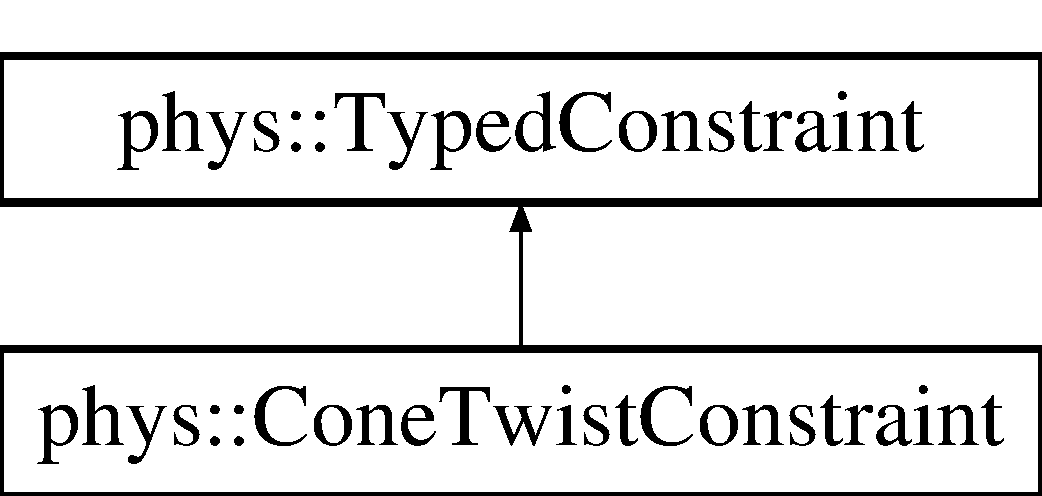
\includegraphics[height=2cm]{da/dbc/classphys_1_1ConeTwistConstraint}
\end{center}
\end{figure}
\subsection*{Public Member Functions}
\begin{DoxyCompactItemize}
\item 
\hypertarget{classphys_1_1ConeTwistConstraint_ab72e1489ea91e47ebbeee41dee116040}{
{\bfseries ConeTwistConstraint} (\hyperlink{classphys_1_1ActorRigid}{ActorRigid} $\ast$ActorA, \hyperlink{classphys_1_1ActorRigid}{ActorRigid} $\ast$ActorB, \hyperlink{classphys_1_1Vector3}{Vector3} VectorA, \hyperlink{classphys_1_1Vector3}{Vector3} Vectorb, \hyperlink{classphys_1_1Quaternion}{Quaternion} QuaternionA, \hyperlink{classphys_1_1Quaternion}{Quaternion} QuaternionB)}
\label{da/dbc/classphys_1_1ConeTwistConstraint_ab72e1489ea91e47ebbeee41dee116040}

\item 
\hypertarget{classphys_1_1ConeTwistConstraint_ab9c2ee7346f1b862d508cbefe22e54e0}{
{\bfseries ConeTwistConstraint} (\hyperlink{classphys_1_1ActorRigid}{ActorRigid} $\ast$ActorA, \hyperlink{classphys_1_1Vector3}{Vector3} VectorA, \hyperlink{classphys_1_1Quaternion}{Quaternion} QuaternionA)}
\label{da/dbc/classphys_1_1ConeTwistConstraint_ab9c2ee7346f1b862d508cbefe22e54e0}

\item 
\hypertarget{classphys_1_1ConeTwistConstraint_a38a9a0e7676d8ad8f77831a319bc007b}{
{\bfseries ConeTwistConstraint} (btConeTwistConstraint $\ast$Constraint)}
\label{da/dbc/classphys_1_1ConeTwistConstraint_a38a9a0e7676d8ad8f77831a319bc007b}

\item 
\hypertarget{classphys_1_1ConeTwistConstraint_a1e2ffb465a8ceab4b77663b9e446a3ae}{
void {\bfseries SetAngularOnly} (bool AngularOnly)}
\label{da/dbc/classphys_1_1ConeTwistConstraint_a1e2ffb465a8ceab4b77663b9e446a3ae}

\item 
\hypertarget{classphys_1_1ConeTwistConstraint_ae8519afb837606a39dfaef447ae96888}{
void {\bfseries SetLimit} (int LimitIndex, \hyperlink{namespacephys_af7eb897198d265b8e868f45240230d5f}{Real} LimitValue)}
\label{da/dbc/classphys_1_1ConeTwistConstraint_ae8519afb837606a39dfaef447ae96888}

\item 
\hypertarget{classphys_1_1ConeTwistConstraint_ac2c48c24f694367a55ed35dd8ed7e10c}{
void {\bfseries SetLimit} (\hyperlink{namespacephys_af7eb897198d265b8e868f45240230d5f}{Real} SwingSpan1, \hyperlink{namespacephys_af7eb897198d265b8e868f45240230d5f}{Real} SwingSpan2, \hyperlink{namespacephys_af7eb897198d265b8e868f45240230d5f}{Real} Twistspan, \hyperlink{namespacephys_af7eb897198d265b8e868f45240230d5f}{Real} Softness=1.0, \hyperlink{namespacephys_af7eb897198d265b8e868f45240230d5f}{Real} BiasFactor=0.3, \hyperlink{namespacephys_af7eb897198d265b8e868f45240230d5f}{Real} RelaxationFactor=1.0)}
\label{da/dbc/classphys_1_1ConeTwistConstraint_ac2c48c24f694367a55ed35dd8ed7e10c}

\item 
\hypertarget{classphys_1_1ConeTwistConstraint_ae93045d83384dccc89f638fa8857caf1}{
void {\bfseries SetDamping} (\hyperlink{namespacephys_af7eb897198d265b8e868f45240230d5f}{Real} Damping)}
\label{da/dbc/classphys_1_1ConeTwistConstraint_ae93045d83384dccc89f638fa8857caf1}

\item 
\hypertarget{classphys_1_1ConeTwistConstraint_a005bf25bd529a03c6678e048941ea83f}{
void {\bfseries SetMaxMotorImpulse} (\hyperlink{namespacephys_af7eb897198d265b8e868f45240230d5f}{Real} MaxMotorImpulse)}
\label{da/dbc/classphys_1_1ConeTwistConstraint_a005bf25bd529a03c6678e048941ea83f}

\item 
\hypertarget{classphys_1_1ConeTwistConstraint_af39f9da7e28591e3361568b3ad1c8eb8}{
void {\bfseries SetMaxMotorImpulseNormalized} (\hyperlink{namespacephys_af7eb897198d265b8e868f45240230d5f}{Real} MaxMotorImpulse)}
\label{da/dbc/classphys_1_1ConeTwistConstraint_af39f9da7e28591e3361568b3ad1c8eb8}

\item 
\hypertarget{classphys_1_1ConeTwistConstraint_a2a2a68b116e99709be83d08dbd3a99f9}{
void {\bfseries SetFixThresh} (\hyperlink{namespacephys_af7eb897198d265b8e868f45240230d5f}{Real} FixThresh)}
\label{da/dbc/classphys_1_1ConeTwistConstraint_a2a2a68b116e99709be83d08dbd3a99f9}

\item 
\hypertarget{classphys_1_1ConeTwistConstraint_a5acf239ac6ff3b5999d81d27ba287414}{
void {\bfseries SetMotorTarget} (\hyperlink{classphys_1_1Quaternion}{Quaternion} Quat)}
\label{da/dbc/classphys_1_1ConeTwistConstraint_a5acf239ac6ff3b5999d81d27ba287414}

\item 
\hypertarget{classphys_1_1ConeTwistConstraint_a4ac6124494fa39770f9fc621e6db3715}{
void {\bfseries SetMotorTargetInConstraintSpace} (\hyperlink{classphys_1_1Quaternion}{Quaternion} Quat)}
\label{da/dbc/classphys_1_1ConeTwistConstraint_a4ac6124494fa39770f9fc621e6db3715}

\item 
\hypertarget{classphys_1_1ConeTwistConstraint_aaf0447bbeeca85fa10959072491cafaf}{
void {\bfseries EnableMotor} (bool Enable)}
\label{da/dbc/classphys_1_1ConeTwistConstraint_aaf0447bbeeca85fa10959072491cafaf}

\item 
\hypertarget{classphys_1_1ConeTwistConstraint_ab7306ac08c3fd61cf88567b4e70702c0}{
bool {\bfseries IsPassedSwingLimit} ()}
\label{da/dbc/classphys_1_1ConeTwistConstraint_ab7306ac08c3fd61cf88567b4e70702c0}

\item 
\hypertarget{classphys_1_1ConeTwistConstraint_a555fc33b10a0c156e0ac93b94587098a}{
virtual void {\bfseries SetParam} (int num, \hyperlink{namespacephys_af7eb897198d265b8e868f45240230d5f}{Real} value, int axis=-\/1)}
\label{da/dbc/classphys_1_1ConeTwistConstraint_a555fc33b10a0c156e0ac93b94587098a}

\item 
\hypertarget{classphys_1_1ConeTwistConstraint_aab54f6c56622cef4314d3bbff194421e}{
virtual \hyperlink{namespacephys_af7eb897198d265b8e868f45240230d5f}{Real} {\bfseries GetParam} (int num, int axis=-\/1)}
\label{da/dbc/classphys_1_1ConeTwistConstraint_aab54f6c56622cef4314d3bbff194421e}

\end{DoxyCompactItemize}
\subsection*{Protected Attributes}
\begin{DoxyCompactItemize}
\item 
\hypertarget{classphys_1_1ConeTwistConstraint_a6bb25f6554b09cc9ce3afb7e1c46f074}{
btConeTwistConstraint $\ast$ {\bfseries ConeTwist}}
\label{da/dbc/classphys_1_1ConeTwistConstraint_a6bb25f6554b09cc9ce3afb7e1c46f074}

\end{DoxyCompactItemize}


\subsection{Detailed Description}


Definition at line 75 of file constraint.h.



The documentation for this class was generated from the following files:\begin{DoxyCompactItemize}
\item 
constraint.h\item 
constraint.cpp\end{DoxyCompactItemize}

\hypertarget{classphys_1_1xml_1_1Document}{
\section{phys::xml::Document Class Reference}
\label{dd/d44/classphys_1_1xml_1_1Document}\index{phys::xml::Document@{phys::xml::Document}}
}
Inheritance diagram for phys::xml::Document:\begin{figure}[H]
\begin{center}
\leavevmode
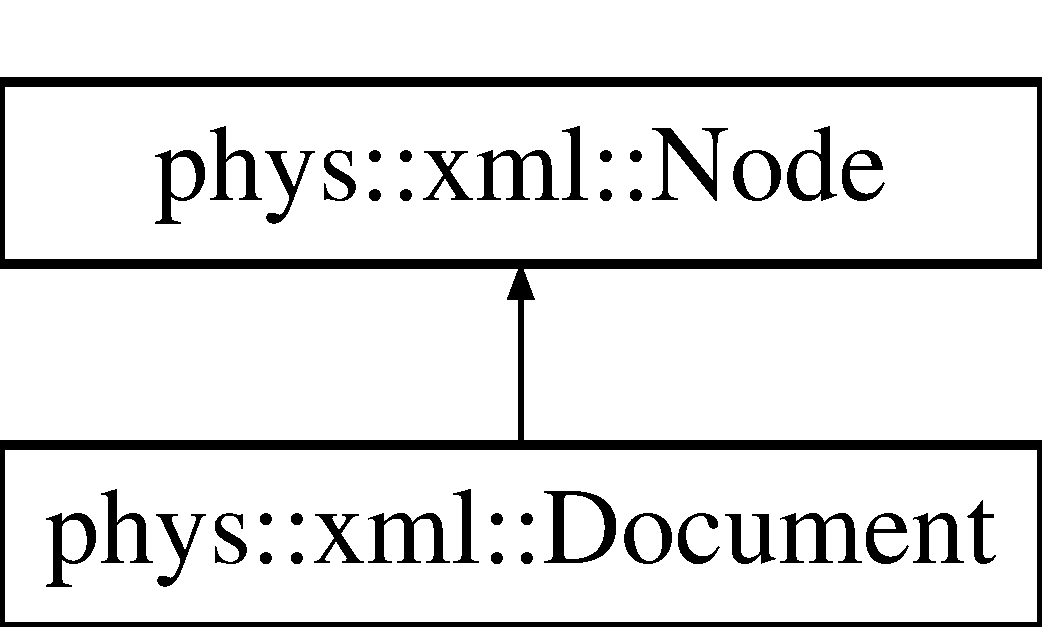
\includegraphics[height=2cm]{dd/d44/classphys_1_1xml_1_1Document}
\end{center}
\end{figure}
\subsection*{Public Member Functions}
\begin{DoxyCompactItemize}
\item 
\hypertarget{classphys_1_1xml_1_1Document_aadb3e68da9cf95b1193f915136f9a7e5}{
void {\bfseries reset} ()}
\label{dd/d44/classphys_1_1xml_1_1Document_aadb3e68da9cf95b1193f915136f9a7e5}

\item 
\hypertarget{classphys_1_1xml_1_1Document_a8d79b0e71457e8a64f331fd4cc117a86}{
void {\bfseries reset} (const \hyperlink{classphys_1_1xml_1_1Document}{Document} \&proto)}
\label{dd/d44/classphys_1_1xml_1_1Document_a8d79b0e71457e8a64f331fd4cc117a86}

\item 
\hypertarget{classphys_1_1xml_1_1Document_ad4b3c84acf2aa57f4ff0a14a1454fdcc}{
\hyperlink{structphys_1_1xml_1_1ParseResult}{ParseResult} {\bfseries load} (std::basic\_\-istream$<$ char, std::char\_\-traits$<$ char $>$ $>$ \&stream, unsigned int options=parse\_\-default, Encoding encoding=encoding\_\-auto)}
\label{dd/d44/classphys_1_1xml_1_1Document_ad4b3c84acf2aa57f4ff0a14a1454fdcc}

\item 
\hypertarget{classphys_1_1xml_1_1Document_a09d74505371b5746d4762daa20a7bb25}{
\hyperlink{structphys_1_1xml_1_1ParseResult}{ParseResult} {\bfseries load} (std::basic\_\-istream$<$ wchar\_\-t, std::char\_\-traits$<$ wchar\_\-t $>$ $>$ \&stream, unsigned int options=parse\_\-default)}
\label{dd/d44/classphys_1_1xml_1_1Document_a09d74505371b5746d4762daa20a7bb25}

\item 
\hypertarget{classphys_1_1xml_1_1Document_a1551e495e2b83897bd8288fc001c6c54}{
\hyperlink{structphys_1_1xml_1_1ParseResult}{ParseResult} {\bfseries load} (const char\_\-t $\ast$contents, unsigned int options=parse\_\-default)}
\label{dd/d44/classphys_1_1xml_1_1Document_a1551e495e2b83897bd8288fc001c6c54}

\item 
\hypertarget{classphys_1_1xml_1_1Document_af208b8bc540a1380c0661ea182f8ee8b}{
\hyperlink{structphys_1_1xml_1_1ParseResult}{ParseResult} {\bfseries load\_\-file} (const char $\ast$path, unsigned int options=parse\_\-default, Encoding encoding=encoding\_\-auto)}
\label{dd/d44/classphys_1_1xml_1_1Document_af208b8bc540a1380c0661ea182f8ee8b}

\item 
\hypertarget{classphys_1_1xml_1_1Document_af39ca4d134cfba6ebdb003a3743586e4}{
\hyperlink{structphys_1_1xml_1_1ParseResult}{ParseResult} {\bfseries load\_\-file} (const wchar\_\-t $\ast$path, unsigned int options=parse\_\-default, Encoding encoding=encoding\_\-auto)}
\label{dd/d44/classphys_1_1xml_1_1Document_af39ca4d134cfba6ebdb003a3743586e4}

\item 
\hypertarget{classphys_1_1xml_1_1Document_a4506ef6f6c98bf43f7e146ab0015a188}{
\hyperlink{structphys_1_1xml_1_1ParseResult}{ParseResult} {\bfseries load\_\-buffer} (const void $\ast$contents, size\_\-t size, unsigned int options=parse\_\-default, Encoding encoding=encoding\_\-auto)}
\label{dd/d44/classphys_1_1xml_1_1Document_a4506ef6f6c98bf43f7e146ab0015a188}

\item 
\hypertarget{classphys_1_1xml_1_1Document_a38beaa65d14eca13dcf6d684be0e6d73}{
\hyperlink{structphys_1_1xml_1_1ParseResult}{ParseResult} {\bfseries load\_\-buffer\_\-inplace} (void $\ast$contents, size\_\-t size, unsigned int options=parse\_\-default, Encoding encoding=encoding\_\-auto)}
\label{dd/d44/classphys_1_1xml_1_1Document_a38beaa65d14eca13dcf6d684be0e6d73}

\item 
\hypertarget{classphys_1_1xml_1_1Document_af29061d7fe8efaa6618b678fd59d0cc6}{
\hyperlink{structphys_1_1xml_1_1ParseResult}{ParseResult} {\bfseries load\_\-buffer\_\-inplace\_\-own} (void $\ast$contents, size\_\-t size, unsigned int options=parse\_\-default, Encoding encoding=encoding\_\-auto)}
\label{dd/d44/classphys_1_1xml_1_1Document_af29061d7fe8efaa6618b678fd59d0cc6}

\item 
\hypertarget{classphys_1_1xml_1_1Document_a8c27a11a0f2f632265f85e292247d2e2}{
void {\bfseries save} (\hyperlink{classphys_1_1xml_1_1Writer}{Writer} \&writer, const char\_\-t $\ast$indent=XML\_\-TEXT(\char`\"{}$\backslash$t\char`\"{}), unsigned int flags=format\_\-default, Encoding encoding=encoding\_\-auto) const }
\label{dd/d44/classphys_1_1xml_1_1Document_a8c27a11a0f2f632265f85e292247d2e2}

\item 
\hypertarget{classphys_1_1xml_1_1Document_addda0a55772282c6887637a7531fc139}{
void {\bfseries save} (std::basic\_\-ostream$<$ char, std::char\_\-traits$<$ char $>$ $>$ \&stream, const char\_\-t $\ast$indent=XML\_\-TEXT(\char`\"{}$\backslash$t\char`\"{}), unsigned int flags=format\_\-default, Encoding encoding=encoding\_\-auto) const }
\label{dd/d44/classphys_1_1xml_1_1Document_addda0a55772282c6887637a7531fc139}

\item 
\hypertarget{classphys_1_1xml_1_1Document_a8bdba6317f7ba369c3c83f2e3f77829a}{
void {\bfseries save} (std::basic\_\-ostream$<$ wchar\_\-t, std::char\_\-traits$<$ wchar\_\-t $>$ $>$ \&stream, const char\_\-t $\ast$indent=XML\_\-TEXT(\char`\"{}$\backslash$t\char`\"{}), unsigned int flags=format\_\-default) const }
\label{dd/d44/classphys_1_1xml_1_1Document_a8bdba6317f7ba369c3c83f2e3f77829a}

\item 
\hypertarget{classphys_1_1xml_1_1Document_ac6eebad9e56a83536fac58d35b49b2e1}{
bool {\bfseries save\_\-file} (const char $\ast$path, const char\_\-t $\ast$indent=XML\_\-TEXT(\char`\"{}$\backslash$t\char`\"{}), unsigned int flags=format\_\-default, Encoding encoding=encoding\_\-auto) const }
\label{dd/d44/classphys_1_1xml_1_1Document_ac6eebad9e56a83536fac58d35b49b2e1}

\item 
\hypertarget{classphys_1_1xml_1_1Document_a67a9fc41324ad4a06f53501eb5b74528}{
bool {\bfseries save\_\-file} (const wchar\_\-t $\ast$path, const char\_\-t $\ast$indent=XML\_\-TEXT(\char`\"{}$\backslash$t\char`\"{}), unsigned int flags=format\_\-default, Encoding encoding=encoding\_\-auto) const }
\label{dd/d44/classphys_1_1xml_1_1Document_a67a9fc41324ad4a06f53501eb5b74528}

\item 
\hypertarget{classphys_1_1xml_1_1Document_a481cbf277cfe6d6daf1b66f8d862b88e}{
\hyperlink{classphys_1_1xml_1_1Node}{Node} {\bfseries document\_\-element} () const }
\label{dd/d44/classphys_1_1xml_1_1Document_a481cbf277cfe6d6daf1b66f8d862b88e}

\end{DoxyCompactItemize}


\subsection{Detailed Description}


Definition at line 791 of file xml.h.



The documentation for this class was generated from the following files:\begin{DoxyCompactItemize}
\item 
\hyperlink{xml_8h}{xml.h}\item 
xml.cpp\end{DoxyCompactItemize}

\hypertarget{classphys_1_1EventBase}{
\section{phys::EventBase Class Reference}
\label{dd/d80/classphys_1_1EventBase}\index{phys::EventBase@{phys::EventBase}}
}


The base class for all events.  




{\ttfamily \#include $<$eventbase.h$>$}

Inheritance diagram for phys::EventBase:\begin{figure}[H]
\begin{center}
\leavevmode
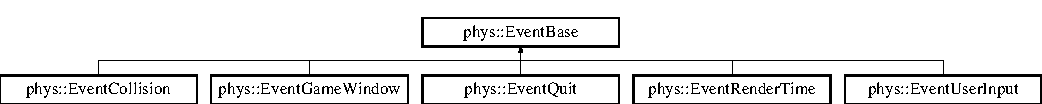
\includegraphics[height=1.842105cm]{dd/d80/classphys_1_1EventBase}
\end{center}
\end{figure}
\subsection*{Public Types}
\begin{DoxyCompactItemize}
\item 
enum \hyperlink{classphys_1_1EventBase_a5e6a8564e127f654123f0bf6a2751923}{EventType} \{ \par
\hyperlink{classphys_1_1EventBase_a5e6a8564e127f654123f0bf6a2751923acdfa47d279e8a1c460d557d14b85c7a5}{RenderTime}, 
\hyperlink{classphys_1_1EventBase_a5e6a8564e127f654123f0bf6a2751923a320cc0817dc2c2201501b12c50c89bef}{UserInput}, 
\hyperlink{classphys_1_1EventBase_a5e6a8564e127f654123f0bf6a2751923a84742ff55e9abdde8f5e0578d30f73a9}{QuitMessage}, 
\hyperlink{classphys_1_1EventBase_a5e6a8564e127f654123f0bf6a2751923a18594400c60af959158e9f5cc2cd5d08}{SystemMessage}, 
\par
\hyperlink{classphys_1_1EventBase_a5e6a8564e127f654123f0bf6a2751923adb6767503168d145497ef65a708725e5}{Collision}, 
{\bfseries Other}
 \}
\end{DoxyCompactItemize}
\subsection*{Public Member Functions}
\begin{DoxyCompactItemize}
\item 
virtual \hyperlink{classphys_1_1EventBase_a5e6a8564e127f654123f0bf6a2751923}{EventBase::EventType} \hyperlink{classphys_1_1EventBase_a1b3d29b6ecf30f18cc3e1825a515c508}{GetType} () const =0
\begin{DoxyCompactList}\small\item\em This will aid in identifying all classes that inherit from this class. \item\end{DoxyCompactList}\end{DoxyCompactItemize}


\subsection{Detailed Description}
The base class for all events. All Events used in the Event Manager, will inherit from this. While not absolutely required by the game programmer to write their own events, it it could be useful. Instances of this class cannot be made, and all classes that inherit from this are expected to implement getEventType(). 

Definition at line 61 of file eventbase.h.



\subsection{Member Enumeration Documentation}
\hypertarget{classphys_1_1EventBase_a5e6a8564e127f654123f0bf6a2751923}{
\index{phys::EventBase@{phys::EventBase}!EventType@{EventType}}
\index{EventType@{EventType}!phys::EventBase@{phys::EventBase}}
\subsubsection[{EventType}]{\setlength{\rightskip}{0pt plus 5cm}enum {\bf phys::EventBase::EventType}}}
\label{dd/d80/classphys_1_1EventBase_a5e6a8564e127f654123f0bf6a2751923}
A listing of values that can be used to identify Events. \begin{Desc}
\item[Enumerator: ]\par
\begin{description}
\index{RenderTime@{RenderTime}!phys::EventBase@{phys::EventBase}}\index{phys::EventBase@{phys::EventBase}!RenderTime@{RenderTime}}\item[{\em 
\hypertarget{classphys_1_1EventBase_a5e6a8564e127f654123f0bf6a2751923acdfa47d279e8a1c460d557d14b85c7a5}{
RenderTime}
\label{dd/d80/classphys_1_1EventBase_a5e6a8564e127f654123f0bf6a2751923acdfa47d279e8a1c460d557d14b85c7a5}
}]Indicates the Event is a PhysEventRenderTime \index{UserInput@{UserInput}!phys::EventBase@{phys::EventBase}}\index{phys::EventBase@{phys::EventBase}!UserInput@{UserInput}}\item[{\em 
\hypertarget{classphys_1_1EventBase_a5e6a8564e127f654123f0bf6a2751923a320cc0817dc2c2201501b12c50c89bef}{
UserInput}
\label{dd/d80/classphys_1_1EventBase_a5e6a8564e127f654123f0bf6a2751923a320cc0817dc2c2201501b12c50c89bef}
}]Indicates the Event is a \hyperlink{classphys_1_1EventUserInput}{EventUserInput} \index{QuitMessage@{QuitMessage}!phys::EventBase@{phys::EventBase}}\index{phys::EventBase@{phys::EventBase}!QuitMessage@{QuitMessage}}\item[{\em 
\hypertarget{classphys_1_1EventBase_a5e6a8564e127f654123f0bf6a2751923a84742ff55e9abdde8f5e0578d30f73a9}{
QuitMessage}
\label{dd/d80/classphys_1_1EventBase_a5e6a8564e127f654123f0bf6a2751923a84742ff55e9abdde8f5e0578d30f73a9}
}]Indicates the Event is a \hyperlink{classphys_1_1EventQuit}{phys::EventQuit} \index{SystemMessage@{SystemMessage}!phys::EventBase@{phys::EventBase}}\index{phys::EventBase@{phys::EventBase}!SystemMessage@{SystemMessage}}\item[{\em 
\hypertarget{classphys_1_1EventBase_a5e6a8564e127f654123f0bf6a2751923a18594400c60af959158e9f5cc2cd5d08}{
SystemMessage}
\label{dd/d80/classphys_1_1EventBase_a5e6a8564e127f654123f0bf6a2751923a18594400c60af959158e9f5cc2cd5d08}
}]Indicates the Event has not been coded yet \index{Collision@{Collision}!phys::EventBase@{phys::EventBase}}\index{phys::EventBase@{phys::EventBase}!Collision@{Collision}}\item[{\em 
\hypertarget{classphys_1_1EventBase_a5e6a8564e127f654123f0bf6a2751923adb6767503168d145497ef65a708725e5}{
Collision}
\label{dd/d80/classphys_1_1EventBase_a5e6a8564e127f654123f0bf6a2751923adb6767503168d145497ef65a708725e5}
}]Indicates the Event is a Physics Collision Event \end{description}
\end{Desc}



Definition at line 67 of file eventbase.h.



\subsection{Member Function Documentation}
\hypertarget{classphys_1_1EventBase_a1b3d29b6ecf30f18cc3e1825a515c508}{
\index{phys::EventBase@{phys::EventBase}!GetType@{GetType}}
\index{GetType@{GetType}!phys::EventBase@{phys::EventBase}}
\subsubsection[{GetType}]{\setlength{\rightskip}{0pt plus 5cm}virtual {\bf EventBase::EventType} phys::EventBase::GetType (
\begin{DoxyParamCaption}
{}
\end{DoxyParamCaption}
) const\hspace{0.3cm}{\ttfamily  \mbox{[}pure virtual\mbox{]}}}}
\label{dd/d80/classphys_1_1EventBase_a1b3d29b6ecf30f18cc3e1825a515c508}


This will aid in identifying all classes that inherit from this class. 

All Classes derived form this calls will return an Event::EventType that correspond the the data/class type they actually are. \begin{DoxyReturn}{Returns}
This returns an eventype that will correspend with the actual event type. This can be used on all Phys game provided class to safely cast a pointer to the correct event type. 
\end{DoxyReturn}


Implemented in \hyperlink{classphys_1_1EventCollision_a96c2809f1bbab78b9f2758cea15a9a36}{phys::EventCollision}, \hyperlink{classphys_1_1EventQuit_a3bfca875349e73dbda47c3c62a253e3b}{phys::EventQuit}, \hyperlink{classphys_1_1EventRenderTime_a160ca55bf9e5a2ae80dab82eab88baf5}{phys::EventRenderTime}, and \hyperlink{classphys_1_1EventUserInput_a3e803a8d9bcc1576fe04d2245a86ec80}{phys::EventUserInput}.



The documentation for this class was generated from the following file:\begin{DoxyCompactItemize}
\item 
eventbase.h\end{DoxyCompactItemize}

\hypertarget{classphys_1_1EventCollision}{
\subsection{phys::EventCollision Class Reference}
\label{dd/de9/classphys_1_1EventCollision}\index{phys::EventCollision@{phys::EventCollision}}
}


This is an event class used to track collsions in the physics world.  




{\ttfamily \#include $<$eventcollision.h$>$}

Inheritance diagram for phys::EventCollision:\begin{figure}[H]
\begin{center}
\leavevmode
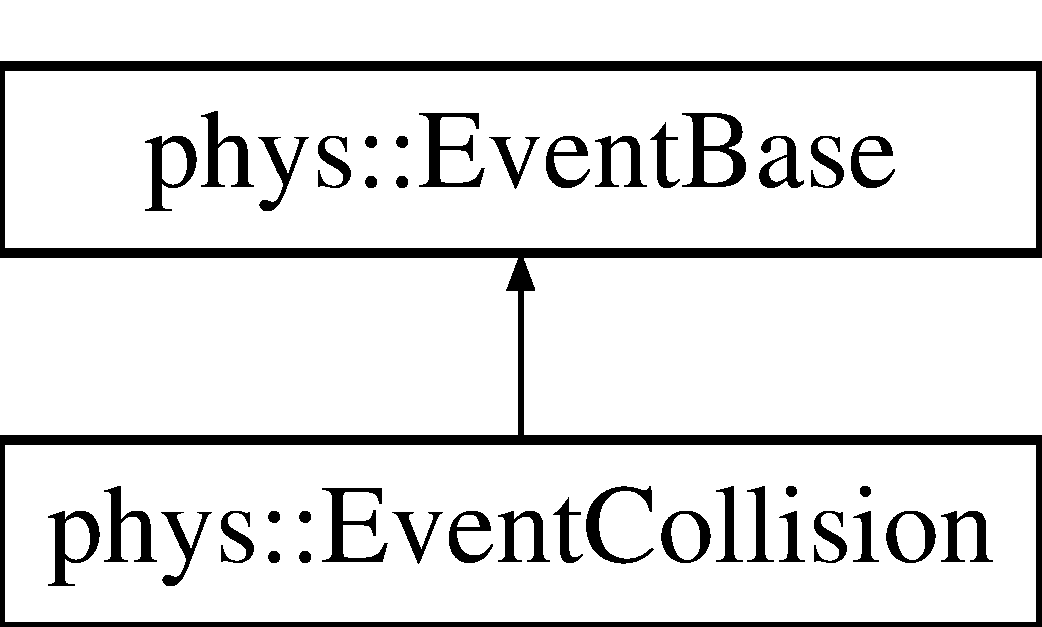
\includegraphics[height=2.000000cm]{dd/de9/classphys_1_1EventCollision}
\end{center}
\end{figure}
\subsubsection*{Public Member Functions}
\begin{DoxyCompactItemize}
\item 
\hypertarget{classphys_1_1EventCollision_af44ef170326f56879e9e4608984a4196}{
\hyperlink{classphys_1_1EventCollision_af44ef170326f56879e9e4608984a4196}{EventCollision} ()}
\label{dd/de9/classphys_1_1EventCollision_af44ef170326f56879e9e4608984a4196}

\begin{DoxyCompactList}\small\item\em Default Constructor. \item\end{DoxyCompactList}\item 
\hyperlink{classphys_1_1EventCollision_a0f5a0862cde3b7db4482be6984434742}{EventCollision} (\hyperlink{classphys_1_1ActorBase}{ActorBase} $\ast$actora, \hyperlink{classphys_1_1ActorBase}{ActorBase} $\ast$actorb, \hyperlink{classphys_1_1Vector3}{Vector3} localAlocation, \hyperlink{classphys_1_1Vector3}{Vector3} localBlocation, \hyperlink{classphys_1_1Vector3}{Vector3} worldlocation, \hyperlink{namespacephys_af7eb897198d265b8e868f45240230d5f}{Real} impulse)
\begin{DoxyCompactList}\small\item\em Class Constructor. \item\end{DoxyCompactList}\item 
\hyperlink{classphys_1_1EventCollision_a85c999154866380d232ddcdfd9534c85}{EventCollision} (const \hyperlink{classphys_1_1EventCollision}{EventCollision} \&Other)
\begin{DoxyCompactList}\small\item\em Copy Constructor. \item\end{DoxyCompactList}\item 
virtual \hyperlink{classphys_1_1EventCollision_afcbf057fc955ce6c05b21c08325b1822}{$\sim$EventCollision} ()
\begin{DoxyCompactList}\small\item\em Class Destructor. \item\end{DoxyCompactList}\item 
virtual \hyperlink{classphys_1_1EventBase_a5e6a8564e127f654123f0bf6a2751923}{EventType} \hyperlink{classphys_1_1EventCollision_a96c2809f1bbab78b9f2758cea15a9a36}{GetType} () const 
\begin{DoxyCompactList}\small\item\em This returns EventType::Collision. \item\end{DoxyCompactList}\end{DoxyCompactItemize}
\subsubsection*{Public Attributes}
\begin{DoxyCompactItemize}
\item 
\hypertarget{classphys_1_1EventCollision_a8f8a80d921bfe1ec24171c5be3ed7641}{
\hyperlink{classphys_1_1Vector3}{Vector3} \hyperlink{classphys_1_1EventCollision_a8f8a80d921bfe1ec24171c5be3ed7641}{WorldLocation}}
\label{dd/de9/classphys_1_1EventCollision_a8f8a80d921bfe1ec24171c5be3ed7641}

\begin{DoxyCompactList}\small\item\em The location in the world where the collision occured. \item\end{DoxyCompactList}\item 
\hypertarget{classphys_1_1EventCollision_a2fa146b8453d2f504abcd5055d2c2a90}{
\hyperlink{classphys_1_1Vector3}{Vector3} \hyperlink{classphys_1_1EventCollision_a2fa146b8453d2f504abcd5055d2c2a90}{LocalALocation}}
\label{dd/de9/classphys_1_1EventCollision_a2fa146b8453d2f504abcd5055d2c2a90}

\begin{DoxyCompactList}\small\item\em The location in ActorA's local space where the collision occured. \item\end{DoxyCompactList}\item 
\hypertarget{classphys_1_1EventCollision_a50d6df6b25532530cd296353ac0b55c6}{
\hyperlink{classphys_1_1Vector3}{Vector3} \hyperlink{classphys_1_1EventCollision_a50d6df6b25532530cd296353ac0b55c6}{LocalBLocation}}
\label{dd/de9/classphys_1_1EventCollision_a50d6df6b25532530cd296353ac0b55c6}

\begin{DoxyCompactList}\small\item\em The location in ActorB's local space where the collision occured. \item\end{DoxyCompactList}\item 
\hypertarget{classphys_1_1EventCollision_a577552db818f54a4092baccf597823a2}{
\hyperlink{namespacephys_af7eb897198d265b8e868f45240230d5f}{Real} \hyperlink{classphys_1_1EventCollision_a577552db818f54a4092baccf597823a2}{Impulse}}
\label{dd/de9/classphys_1_1EventCollision_a577552db818f54a4092baccf597823a2}

\begin{DoxyCompactList}\small\item\em The amount of force of the collision. \item\end{DoxyCompactList}\item 
\hypertarget{classphys_1_1EventCollision_a2de905d0332c66293cbe990fe2dbbb07}{
\hyperlink{classphys_1_1ActorBase}{ActorBase} $\ast$ \hyperlink{classphys_1_1EventCollision_a2de905d0332c66293cbe990fe2dbbb07}{ActorA}}
\label{dd/de9/classphys_1_1EventCollision_a2de905d0332c66293cbe990fe2dbbb07}

\begin{DoxyCompactList}\small\item\em The first Actor involved in the collision. \item\end{DoxyCompactList}\item 
\hypertarget{classphys_1_1EventCollision_a922fd42b74db6df7a59cb5fd54cbadbe}{
\hyperlink{classphys_1_1ActorBase}{ActorBase} $\ast$ \hyperlink{classphys_1_1EventCollision_a922fd42b74db6df7a59cb5fd54cbadbe}{ActorB}}
\label{dd/de9/classphys_1_1EventCollision_a922fd42b74db6df7a59cb5fd54cbadbe}

\begin{DoxyCompactList}\small\item\em The second Actor invovled in the collision. \item\end{DoxyCompactList}\end{DoxyCompactItemize}


\subsubsection{Detailed Description}
This is an event class used to track collsions in the physics world. This class will be used for tracking collisions in the physics world and will keep track of basic data related to the collision. 

Definition at line 55 of file eventcollision.h.



\subsubsection{Constructor \& Destructor Documentation}
\hypertarget{classphys_1_1EventCollision_a0f5a0862cde3b7db4482be6984434742}{
\index{phys::EventCollision@{phys::EventCollision}!EventCollision@{EventCollision}}
\index{EventCollision@{EventCollision}!phys::EventCollision@{phys::EventCollision}}
\paragraph[{EventCollision}]{\setlength{\rightskip}{0pt plus 5cm}phys::EventCollision::EventCollision (
\begin{DoxyParamCaption}
\item[{{\bf ActorBase} $\ast$}]{ actora, }
\item[{{\bf ActorBase} $\ast$}]{ actorb, }
\item[{{\bf Vector3}}]{ localAlocation, }
\item[{{\bf Vector3}}]{ localBlocation, }
\item[{{\bf Vector3}}]{ worldlocation, }
\item[{{\bf Real}}]{ impulse}
\end{DoxyParamCaption}
)}\hfill}
\label{dd/de9/classphys_1_1EventCollision_a0f5a0862cde3b7db4482be6984434742}


Class Constructor. 

This will construct a basic event class with the minimum data needed. 
\begin{DoxyParams}{Parameters}
\item[{\em actora}]The first Actor involved in the collision. \item[{\em actorb}]The second Actor invovled in the collision. \item[{\em localAlocation}]The location in ActorA's local space where the collision occured. \item[{\em localBlocation}]The location in ActorB's local space where the collision occured. \item[{\em worldlocation}]The location in the world where the collision occured. \item[{\em impulse}]The amount of force of the collision. \end{DoxyParams}


Definition at line 60 of file eventcollision.cpp.

\hypertarget{classphys_1_1EventCollision_a85c999154866380d232ddcdfd9534c85}{
\index{phys::EventCollision@{phys::EventCollision}!EventCollision@{EventCollision}}
\index{EventCollision@{EventCollision}!phys::EventCollision@{phys::EventCollision}}
\paragraph[{EventCollision}]{\setlength{\rightskip}{0pt plus 5cm}phys::EventCollision::EventCollision (
\begin{DoxyParamCaption}
\item[{const {\bf EventCollision} \&}]{ Other}
\end{DoxyParamCaption}
)}\hfill}
\label{dd/de9/classphys_1_1EventCollision_a85c999154866380d232ddcdfd9534c85}


Copy Constructor. 


\begin{DoxyParams}{Parameters}
\item[{\em Other}]The other \hyperlink{classphys_1_1EventCollision}{EventCollision} to copy \end{DoxyParams}


Definition at line 70 of file eventcollision.cpp.

\hypertarget{classphys_1_1EventCollision_afcbf057fc955ce6c05b21c08325b1822}{
\index{phys::EventCollision@{phys::EventCollision}!$\sim$EventCollision@{$\sim$EventCollision}}
\index{$\sim$EventCollision@{$\sim$EventCollision}!phys::EventCollision@{phys::EventCollision}}
\paragraph[{$\sim$EventCollision}]{\setlength{\rightskip}{0pt plus 5cm}phys::EventCollision::$\sim$EventCollision (
\begin{DoxyParamCaption}
{}
\end{DoxyParamCaption}
)\hspace{0.3cm}{\ttfamily  \mbox{[}virtual\mbox{]}}}\hfill}
\label{dd/de9/classphys_1_1EventCollision_afcbf057fc955ce6c05b21c08325b1822}


Class Destructor. 

Basic Class Destructor. 

Definition at line 80 of file eventcollision.cpp.



\subsubsection{Member Function Documentation}
\hypertarget{classphys_1_1EventCollision_a96c2809f1bbab78b9f2758cea15a9a36}{
\index{phys::EventCollision@{phys::EventCollision}!GetType@{GetType}}
\index{GetType@{GetType}!phys::EventCollision@{phys::EventCollision}}
\paragraph[{GetType}]{\setlength{\rightskip}{0pt plus 5cm}{\bf EventBase::EventType} phys::EventCollision::GetType (
\begin{DoxyParamCaption}
{}
\end{DoxyParamCaption}
) const\hspace{0.3cm}{\ttfamily  \mbox{[}virtual\mbox{]}}}\hfill}
\label{dd/de9/classphys_1_1EventCollision_a96c2809f1bbab78b9f2758cea15a9a36}


This returns EventType::Collision. 

This returns the kind of message this is, specifcally EventType::Collision. This method is inherited from phys::Event. . 

Implements \hyperlink{classphys_1_1EventBase_a1b3d29b6ecf30f18cc3e1825a515c508}{phys::EventBase}.



Definition at line 84 of file eventcollision.cpp.



The documentation for this class was generated from the following files:\begin{DoxyCompactItemize}
\item 
eventcollision.h\item 
eventcollision.cpp\end{DoxyCompactItemize}

\hypertarget{classphys_1_1EventManager}{
\subsection{phys::EventManager Class Reference}
\label{classphys_1_1EventManager}\index{phys::EventManager@{phys::EventManager}}
}


This is a container for Events and facilitates the transfer of data.  




{\ttfamily \#include $<$eventmanager.h$>$}

Inheritance diagram for phys::EventManager:\begin{figure}[H]
\begin{center}
\leavevmode
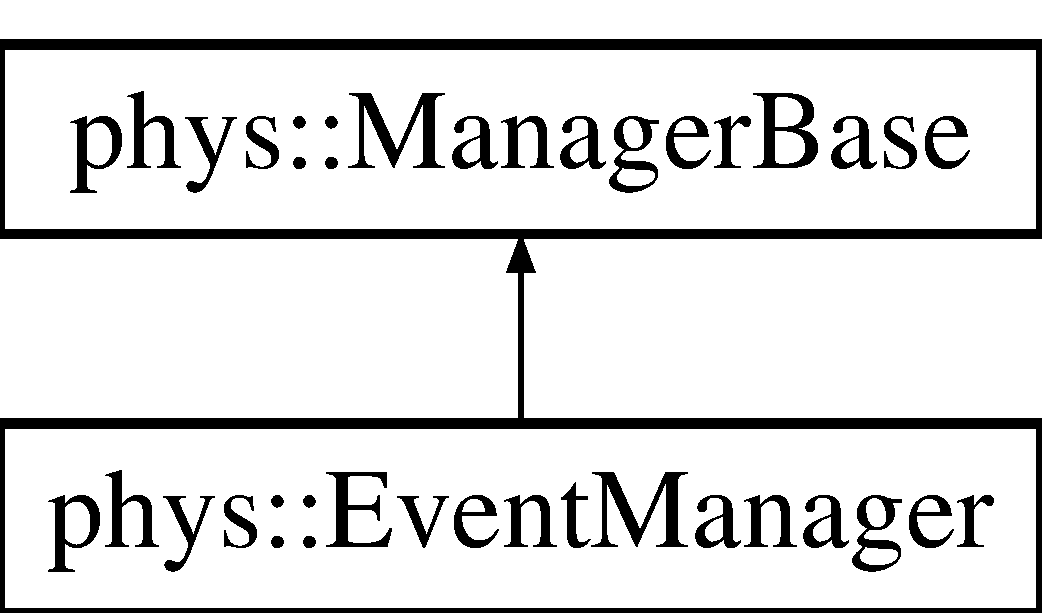
\includegraphics[height=2.000000cm]{classphys_1_1EventManager}
\end{center}
\end{figure}
\subsubsection*{Public Member Functions}
\begin{DoxyCompactItemize}
\item 
void \hyperlink{classphys_1_1EventManager_abada23d83ef38e59a38eb91a88a07404}{AddEvent} (\hyperlink{classphys_1_1EventBase}{EventBase} $\ast$EventToAdd)
\begin{DoxyCompactList}\small\item\em Adds an event of any kind to the end of the Event Queue. \item\end{DoxyCompactList}\item 
void \hyperlink{classphys_1_1EventManager_a6ff66883358344908afd11204f79f196}{AddPollingCheck} (const \hyperlink{classphys_1_1MetaCode}{MetaCode} \&InputToTryPolling)
\begin{DoxyCompactList}\small\item\em Generates extra events each iteration of the main loop, based on user input polling. \item\end{DoxyCompactList}\item 
void \hyperlink{classphys_1_1EventManager_a0b36c605c2a059c96e787ed4c1fd68bc}{DetectJoysticks} ()
\begin{DoxyCompactList}\small\item\em Look for Joysticks that are hooked up to the system. \item\end{DoxyCompactList}\item 
virtual void \hyperlink{classphys_1_1EventManager_aca8fb3d285484dcdb943824bf11f3596}{DoMainLoopItems} ()
\begin{DoxyCompactList}\small\item\em Empty MainLoopItems. \item\end{DoxyCompactList}\item 
\hyperlink{classphys_1_1EventManager_a018b36588bf2a2e90536e64be060d6fc}{EventManager} ()
\begin{DoxyCompactList}\small\item\em Default constructor. \item\end{DoxyCompactList}\item 
std::list$<$ \hyperlink{classphys_1_1EventCollision}{EventCollision} $\ast$ $>$ $\ast$ \hyperlink{classphys_1_1EventManager_a1881421e075a5965d6d5a0678f93ad9a}{GetAllCollisionEvents} ()
\begin{DoxyCompactList}\small\item\em This returns a complete list of all the Render \hyperlink{structphys_1_1Time}{Time} events. \item\end{DoxyCompactList}\item 
std::list$<$ \hyperlink{classphys_1_1EventGameWindow}{EventGameWindow} $\ast$ $>$ $\ast$ \hyperlink{classphys_1_1EventManager_aacdd185f6334f1258d0d7022bae3932d}{GetAllGameWindowEvents} ()
\begin{DoxyCompactList}\small\item\em This returns a complete list of all the Render \hyperlink{structphys_1_1Time}{Time} events. \item\end{DoxyCompactList}\item 
std::list$<$ \hyperlink{classphys_1_1EventQuit}{EventQuit} $\ast$ $>$ $\ast$ \hyperlink{classphys_1_1EventManager_afefd52a9693bc5541592997abbf3c53f}{GetAllQuitEvents} ()
\begin{DoxyCompactList}\small\item\em This returns a complete list of all the quit events. \item\end{DoxyCompactList}\item 
std::list$<$ \hyperlink{classphys_1_1EventRenderTime}{EventRenderTime} $\ast$ $>$ $\ast$ \hyperlink{classphys_1_1EventManager_aee73dff2d113826b8c01db7f7417d527}{GetAllRenderTimeEvents} ()
\begin{DoxyCompactList}\small\item\em This returns a complete list of all the Render \hyperlink{structphys_1_1Time}{Time} events. \item\end{DoxyCompactList}\item 
std::list$<$ \hyperlink{classphys_1_1EventBase}{EventBase} $\ast$ $>$ $\ast$ \hyperlink{classphys_1_1EventManager_a300e537d27cd53ac8276438d4c91a3f6}{GetAllSpecificEvents} (\hyperlink{classphys_1_1EventBase_a5e6a8564e127f654123f0bf6a2751923}{EventBase::EventType} SpecificType)
\begin{DoxyCompactList}\small\item\em This returns a complete list of all the specified events. \item\end{DoxyCompactList}\item 
std::list$<$ \hyperlink{classphys_1_1EventUserInput}{EventUserInput} $\ast$ $>$ $\ast$ \hyperlink{classphys_1_1EventManager_aef240dacae9479c4385d540e4feab867}{GetAllUserInputEvents} ()
\begin{DoxyCompactList}\small\item\em This returns a complete list of all the User Input events. \item\end{DoxyCompactList}\item 
\hyperlink{classphys_1_1EventCollision}{EventCollision} $\ast$ \hyperlink{classphys_1_1EventManager_a8e8f88684cd9167ae59734cf14b64b76}{GetNextCollisionEvent} ()
\begin{DoxyCompactList}\small\item\em Returns a pointer to the Next Collision event. \item\end{DoxyCompactList}\item 
\hyperlink{classphys_1_1EventBase}{EventBase} $\ast$ \hyperlink{classphys_1_1EventManager_aa0937763961aefc59aea197a8f9bc0dc}{GetNextEvent} ()
\begin{DoxyCompactList}\small\item\em Return a pointer to the Next event. \item\end{DoxyCompactList}\item 
\hyperlink{classphys_1_1EventGameWindow}{EventGameWindow} $\ast$ \hyperlink{classphys_1_1EventManager_aead881349edba3f0bcca34eaae41a8ee}{GetNextGameWindowEvent} ()
\begin{DoxyCompactList}\small\item\em Returns a pointer to the Next \hyperlink{classphys_1_1GameWindow}{GameWindow} event. \item\end{DoxyCompactList}\item 
\hyperlink{classphys_1_1EventQuit}{EventQuit} $\ast$ \hyperlink{classphys_1_1EventManager_ad7da09e5422b1db79ac4187ee9198d0c}{GetNextQuitEvent} ()
\begin{DoxyCompactList}\small\item\em Returns a pointer to the Next \hyperlink{classphys_1_1EventQuit}{EventQuit}. \item\end{DoxyCompactList}\item 
\hyperlink{classphys_1_1EventRenderTime}{EventRenderTime} $\ast$ \hyperlink{classphys_1_1EventManager_ae8730b039a280449af052d75f2e60b06}{GetNextRenderTimeEvent} ()
\begin{DoxyCompactList}\small\item\em Returns a pointer to the Next Rendertime event. \item\end{DoxyCompactList}\item 
\hyperlink{classphys_1_1EventBase}{EventBase} $\ast$ \hyperlink{classphys_1_1EventManager_a7340cfab326856cf4ebc653b11101016}{GetNextSpecificEvent} (\hyperlink{classphys_1_1EventBase_a5e6a8564e127f654123f0bf6a2751923}{EventBase::EventType} SpecificType)
\begin{DoxyCompactList}\small\item\em Returns a pointer to the Next kind event of the Specified type. \item\end{DoxyCompactList}\item 
\hyperlink{classphys_1_1EventUserInput}{EventUserInput} $\ast$ \hyperlink{classphys_1_1EventManager_a38b42602a3a4d621048c78b525b4db49}{GetNextUserInputEvent} ()
\begin{DoxyCompactList}\small\item\em Returns a pointer to the Next User Input event. \item\end{DoxyCompactList}\item 
size\_\-t \hyperlink{classphys_1_1EventManager_af3e02562344e4de9c40d91446acd84dc}{GetRemainingEventCount} ()
\begin{DoxyCompactList}\small\item\em Gets a count of events. \item\end{DoxyCompactList}\item 
virtual \hyperlink{classphys_1_1ManagerBase_aaa6ccddf23892eaccb898529414f80a5}{ManagerTypeName} \hyperlink{classphys_1_1EventManager_a194890f7f8be5d45aa98623481482696}{GetType} () const 
\begin{DoxyCompactList}\small\item\em This returns the type of this manager. \item\end{DoxyCompactList}\item 
virtual void \hyperlink{classphys_1_1EventManager_a51afdd83f44f461dfac5c9eca5883ea0}{Initialize} ()
\begin{DoxyCompactList}\small\item\em Empty Initializer. \item\end{DoxyCompactList}\item 
\hyperlink{classphys_1_1EventCollision}{EventCollision} $\ast$ \hyperlink{classphys_1_1EventManager_a6a6ae165032e429c12653565590040cd}{PopNextCollisionEvent} ()
\begin{DoxyCompactList}\small\item\em Returns a pointer to the Next Collision event and removes it from the Que. \item\end{DoxyCompactList}\item 
\hyperlink{classphys_1_1EventBase}{EventBase} $\ast$ \hyperlink{classphys_1_1EventManager_ae403b203bc425744377ec5fc311f4e5d}{PopNextEvent} ()
\begin{DoxyCompactList}\small\item\em Return a pointer to the Next event, and removes the Event from storage. \item\end{DoxyCompactList}\item 
\hyperlink{classphys_1_1EventGameWindow}{EventGameWindow} $\ast$ \hyperlink{classphys_1_1EventManager_abc62c29549957c314a8784eac4fb16ad}{PopNextGameWindowEvent} ()
\begin{DoxyCompactList}\small\item\em Returns a pointer to the Next \hyperlink{classphys_1_1GameWindow}{GameWindow} event and removes it from the Que. \item\end{DoxyCompactList}\item 
\hyperlink{classphys_1_1EventQuit}{EventQuit} $\ast$ \hyperlink{classphys_1_1EventManager_a9b0d8e4d76fef35423bb862d7127b747}{PopNextQuitEvent} ()
\begin{DoxyCompactList}\small\item\em Returns a pointer to the Next \hyperlink{classphys_1_1EventQuit}{EventQuit} and removes it from the Que. \item\end{DoxyCompactList}\item 
\hyperlink{classphys_1_1EventRenderTime}{EventRenderTime} $\ast$ \hyperlink{classphys_1_1EventManager_aa7e800d34ad8b9295ac87dfa822a2a03}{PopNextRenderTimeEvent} ()
\begin{DoxyCompactList}\small\item\em Returns a pointer to the Next Rendertime event and removes it from the Que. \item\end{DoxyCompactList}\item 
\hyperlink{classphys_1_1EventBase}{EventBase} $\ast$ \hyperlink{classphys_1_1EventManager_a156ba3c53cc799499272430111bbdfa4}{PopNextSpecificEvent} (\hyperlink{classphys_1_1EventBase_a5e6a8564e127f654123f0bf6a2751923}{EventBase::EventType} SpecificType)
\begin{DoxyCompactList}\small\item\em Returns a pointer to the Next kind event of the Specified type, and removes it from the Que. \item\end{DoxyCompactList}\item 
\hyperlink{classphys_1_1EventUserInput}{EventUserInput} $\ast$ \hyperlink{classphys_1_1EventManager_afa89317d4b16c2b7065b9f79a4354654}{PopNextUserInputEvent} ()
\begin{DoxyCompactList}\small\item\em Returns a pointer to the Next User Input event and removes it from the Que. \item\end{DoxyCompactList}\item 
void \hyperlink{classphys_1_1EventManager_ac38a5a7d003a3f92e40c842916094bde}{RemoveAllSpecificEvents} (\hyperlink{classphys_1_1EventBase_a5e6a8564e127f654123f0bf6a2751923}{EventBase::EventType} SpecificType)
\begin{DoxyCompactList}\small\item\em This removes all the events of the specified type. \item\end{DoxyCompactList}\item 
void \hyperlink{classphys_1_1EventManager_a9556b702c4b84bc8e49f1491104b688f}{RemoveNextCollisionEvent} ()
\begin{DoxyCompactList}\small\item\em Removes the First Collision Event From the que without looking at it. \item\end{DoxyCompactList}\item 
void \hyperlink{classphys_1_1EventManager_a2389a44d199f121e1fea741f83248513}{RemoveNextEvent} ()
\begin{DoxyCompactList}\small\item\em Removes an Event From the que without looking at it. \item\end{DoxyCompactList}\item 
void \hyperlink{classphys_1_1EventManager_a8172d685143bf18d0e48810fac25860e}{RemoveNextGameWindowEvent} ()
\begin{DoxyCompactList}\small\item\em Removes the First \hyperlink{classphys_1_1GameWindow}{GameWindow} Event From the que without looking at it. \item\end{DoxyCompactList}\item 
void \hyperlink{classphys_1_1EventManager_a5031871aa6e044764ec2963228f735dd}{RemoveNextQuitEvent} ()
\begin{DoxyCompactList}\small\item\em Removes the First \hyperlink{classphys_1_1EventQuit}{EventQuit} From the que without looking at it. \item\end{DoxyCompactList}\item 
void \hyperlink{classphys_1_1EventManager_af1204912be3554312e66d3a777c1f99b}{RemoveNextRenderTimeEvent} ()
\begin{DoxyCompactList}\small\item\em Removes the First Rendertime Event From the que without looking at it. \item\end{DoxyCompactList}\item 
void \hyperlink{classphys_1_1EventManager_a486c1173a2c1a64885bfdbe7ca267611}{RemoveNextSpecificEvent} (\hyperlink{classphys_1_1EventBase_a5e6a8564e127f654123f0bf6a2751923}{EventBase::EventType} SpecificType)
\begin{DoxyCompactList}\small\item\em Returns a pointer to the Next kind event of the Specified type, and removes it from the Que. \item\end{DoxyCompactList}\item 
void \hyperlink{classphys_1_1EventManager_add41b5f4d2942461bcaf40a97ad40b09}{RemoveNextUserInputEvent} ()
\begin{DoxyCompactList}\small\item\em Removes the First User Input Event From the que without looking at it. \item\end{DoxyCompactList}\item 
void \hyperlink{classphys_1_1EventManager_adaf7d5346932506ed43f893eb071fd39}{RemovePollingCheck} (const \hyperlink{classphys_1_1MetaCode}{MetaCode} \&InputToStopPolling)
\begin{DoxyCompactList}\small\item\em Removes Events from the list(s) of what needs to be polled. \item\end{DoxyCompactList}\item 
void \hyperlink{classphys_1_1EventManager_a63cf23dc9fe0ced3e2c60ca61c97b166}{UpdateEvents} ()
\begin{DoxyCompactList}\small\item\em Pulls Events from the all the subsystems for use in the \hyperlink{classphys_1_1EventManager}{EventManager}. \item\end{DoxyCompactList}\item 
\hyperlink{classphys_1_1EventManager_aa6df8df9b7a11dadcd9bc79ecdf54558}{$\sim$EventManager} ()
\begin{DoxyCompactList}\small\item\em Default Deconstructor. \item\end{DoxyCompactList}\end{DoxyCompactItemize}
\subsubsection*{Friends}
\begin{DoxyCompactItemize}
\item 
\hypertarget{classphys_1_1EventManager_ad68113acdef0b428e8180ee4192aca09}{
std::ostream \& {\bfseries PHYS\_\-LIB::operator$<$$<$} (std::ostream \&stream, const \hyperlink{classphys_1_1EventManager}{phys::EventManager} \&Mgr)}
\label{classphys_1_1EventManager_ad68113acdef0b428e8180ee4192aca09}

\item 
\hypertarget{classphys_1_1EventManager_a04e666d9104e325839dc9a6e63cd3c6f}{
void {\bfseries PHYS\_\-LIB::operator$>$$>$} (const \hyperlink{classphys_1_1xml_1_1Node}{phys::xml::Node} \&OneNode, \hyperlink{classphys_1_1EventManager}{phys::EventManager} \&Mgr)}
\label{classphys_1_1EventManager_a04e666d9104e325839dc9a6e63cd3c6f}

\item 
\hypertarget{classphys_1_1EventManager_ac32b5a1ad8a8171298bd544eda444865}{
std::istream \& {\bfseries PHYS\_\-LIB::operator$>$$>$} (std::istream \&stream, \hyperlink{classphys_1_1EventManager}{phys::EventManager} \&Mgr)}
\label{classphys_1_1EventManager_ac32b5a1ad8a8171298bd544eda444865}

\end{DoxyCompactItemize}


\subsubsection{Detailed Description}
This is a container for Events and facilitates the transfer of data. The Event Manager Exists to passed important information about Gamestate from where it is generated to where it is needed. It is the Game Developers option whether they want to grab events directly using the get functions that have filters, or if they want to get all the events at once from a central location and dispatch form there. \par
 Since all User input comes in the form of events, this is also where user input Polling and optional input sources like Joysticks are controlled from. \par
 All of these event are stored in an internal Queue and order is preserved. So the First item In will be the First Out (FIFO). This is not strictly a FIFO buffer, there are a number of functions for getting of managing specific kinds of events. Generally these 'Filtered' management functions Still return the first of those kinds of event. \begin{DoxyWarning}{Warning}
Delete pointers you get from this. Anything can create events and Put them here, and anything can get them out, This means the simple way to not cause memory leaks is to have the routines extracting the events delete the events. 

Currently this is not thread safe, even though it should be. 
\end{DoxyWarning}


Definition at line 127 of file eventmanager.h.



\subsubsection{Constructor \& Destructor Documentation}
\hypertarget{classphys_1_1EventManager_a018b36588bf2a2e90536e64be060d6fc}{
\index{phys::EventManager@{phys::EventManager}!EventManager@{EventManager}}
\index{EventManager@{EventManager}!phys::EventManager@{phys::EventManager}}
\paragraph[{EventManager}]{\setlength{\rightskip}{0pt plus 5cm}phys::EventManager::EventManager (
\begin{DoxyParamCaption}
{}
\end{DoxyParamCaption}
)}\hfill}
\label{classphys_1_1EventManager_a018b36588bf2a2e90536e64be060d6fc}


Default constructor. 

This creates an empty PhysEventManger

\begin{Desc}
\item[\hyperlink{todo__todo000009}{Todo}]TODO: Make the \hyperlink{classphys_1_1EventManager}{EventManager} completely thread safe. IF this is completely thread safe, we can spawn numerous individual thread each accessing this and and the performance gain would almost scale directly with cpu core count increases. Look at boost scoped\_\-lock \end{Desc}


Definition at line 251 of file eventmanager.cpp.

\hypertarget{classphys_1_1EventManager_aa6df8df9b7a11dadcd9bc79ecdf54558}{
\index{phys::EventManager@{phys::EventManager}!$\sim$EventManager@{$\sim$EventManager}}
\index{$\sim$EventManager@{$\sim$EventManager}!phys::EventManager@{phys::EventManager}}
\paragraph[{$\sim$EventManager}]{\setlength{\rightskip}{0pt plus 5cm}phys::EventManager::$\sim$EventManager (
\begin{DoxyParamCaption}
{}
\end{DoxyParamCaption}
)}\hfill}
\label{classphys_1_1EventManager_aa6df8df9b7a11dadcd9bc79ecdf54558}


Default Deconstructor. 

This deletes everything still in the event manager and tears it down. 

Definition at line 263 of file eventmanager.cpp.



\subsubsection{Member Function Documentation}
\hypertarget{classphys_1_1EventManager_abada23d83ef38e59a38eb91a88a07404}{
\index{phys::EventManager@{phys::EventManager}!AddEvent@{AddEvent}}
\index{AddEvent@{AddEvent}!phys::EventManager@{phys::EventManager}}
\paragraph[{AddEvent}]{\setlength{\rightskip}{0pt plus 5cm}void phys::EventManager::AddEvent (
\begin{DoxyParamCaption}
\item[{{\bf EventBase} $\ast$}]{EventToAdd}
\end{DoxyParamCaption}
)}\hfill}
\label{classphys_1_1EventManager_abada23d83ef38e59a38eb91a88a07404}


Adds an event of any kind to the end of the Event Queue. 


\begin{DoxyParams}{Parameters}
{\em EventToAdd} & This is a pointer to an Event.\\
\hline
\end{DoxyParams}
This adds the existing event to the Queue. Be careful this is not delete, and does not go out of scope. Deleting the Event is now the responsibilty of the code that pulls it out of Event Manager. 

Definition at line 307 of file eventmanager.cpp.

\hypertarget{classphys_1_1EventManager_a6ff66883358344908afd11204f79f196}{
\index{phys::EventManager@{phys::EventManager}!AddPollingCheck@{AddPollingCheck}}
\index{AddPollingCheck@{AddPollingCheck}!phys::EventManager@{phys::EventManager}}
\paragraph[{AddPollingCheck}]{\setlength{\rightskip}{0pt plus 5cm}void phys::EventManager::AddPollingCheck (
\begin{DoxyParamCaption}
\item[{const {\bf MetaCode} \&}]{InputToTryPolling}
\end{DoxyParamCaption}
)}\hfill}
\label{classphys_1_1EventManager_a6ff66883358344908afd11204f79f196}


Generates extra events each iteration of the main loop, based on user input polling. 


\begin{DoxyParams}{Parameters}
{\em InputToTryPolling} & This accepts a \hyperlink{classphys_1_1MetaCode}{MetaCode} and will try to watch for occurences like this one\\
\hline
\end{DoxyParams}
This will trigger the input system to generate an event (or add to an exiting event) when polling for the given kind of event. Each Iteration of the main loop there will be a \hyperlink{classphys_1_1EventUserInput}{EventUserInput} that created. That Event will Include all the normal metacodes for user input that happened, and it will also have a meta code for each time this function was called. The added metacode may be partialky ignored, the Metavalue is almost always ignored, and in a situation where the can only be one of a given input on a system, the ID is ignore and 0 is assumed. 
\begin{DoxyExceptions}{Exceptions}
{\em Unsupported Polling Check on this Platform} & When the metacode passed cannot be polled on this platform \\
\hline
\end{DoxyExceptions}


Definition at line 606 of file eventmanager.cpp.

\hypertarget{classphys_1_1EventManager_a0b36c605c2a059c96e787ed4c1fd68bc}{
\index{phys::EventManager@{phys::EventManager}!DetectJoysticks@{DetectJoysticks}}
\index{DetectJoysticks@{DetectJoysticks}!phys::EventManager@{phys::EventManager}}
\paragraph[{DetectJoysticks}]{\setlength{\rightskip}{0pt plus 5cm}void phys::EventManager::DetectJoysticks (
\begin{DoxyParamCaption}
{}
\end{DoxyParamCaption}
)}\hfill}
\label{classphys_1_1EventManager_a0b36c605c2a059c96e787ed4c1fd68bc}


Look for Joysticks that are hooked up to the system. 

Currently this will only find the first joystick. This only needs to be done once after the joystick has been connected and detected/configured by the operating system. Joystick events may not be added if this has not been called. The is called once at when the Event manager is contructed, but if the joystick was not connected yet then it might not be found. 

Definition at line 275 of file eventmanager.cpp.

\hypertarget{classphys_1_1EventManager_aca8fb3d285484dcdb943824bf11f3596}{
\index{phys::EventManager@{phys::EventManager}!DoMainLoopItems@{DoMainLoopItems}}
\index{DoMainLoopItems@{DoMainLoopItems}!phys::EventManager@{phys::EventManager}}
\paragraph[{DoMainLoopItems}]{\setlength{\rightskip}{0pt plus 5cm}void phys::EventManager::DoMainLoopItems (
\begin{DoxyParamCaption}
{}
\end{DoxyParamCaption}
)\hspace{0.3cm}{\ttfamily  \mbox{[}virtual\mbox{]}}}\hfill}
\label{classphys_1_1EventManager_aca8fb3d285484dcdb943824bf11f3596}


Empty MainLoopItems. 

This class implements this for the sake of entension and compatibility this function does nothing. This is just empty during this round of refactoring, and this will get all the functionality that currently should be here, but is in the world 

Implements \hyperlink{classphys_1_1ManagerBase_aa9e13a3f7c398b708f0f242610b5abf7}{phys::ManagerBase}.



Definition at line 644 of file eventmanager.cpp.

\hypertarget{classphys_1_1EventManager_a1881421e075a5965d6d5a0678f93ad9a}{
\index{phys::EventManager@{phys::EventManager}!GetAllCollisionEvents@{GetAllCollisionEvents}}
\index{GetAllCollisionEvents@{GetAllCollisionEvents}!phys::EventManager@{phys::EventManager}}
\paragraph[{GetAllCollisionEvents}]{\setlength{\rightskip}{0pt plus 5cm}std::list$<$ {\bf EventCollision} $\ast$ $>$ $\ast$ phys::EventManager::GetAllCollisionEvents (
\begin{DoxyParamCaption}
{}
\end{DoxyParamCaption}
)}\hfill}
\label{classphys_1_1EventManager_a1881421e075a5965d6d5a0678f93ad9a}


This returns a complete list of all the Render \hyperlink{structphys_1_1Time}{Time} events. 

This finds all the \hyperlink{classphys_1_1EventUserInput}{EventUserInput} Events then creates a new list and returns that. This runs in linear time relative to the amounts of events. \begin{DoxyReturn}{Returns}
This returns a list$<$EventCollision$\ast$$>$ pointer which is this a subset of this classes event pointer list. Use this carefully, it can cause errors if used improperly. This list pointer must be deleted, but not the events in it. 
\end{DoxyReturn}


Definition at line 538 of file eventmanager.cpp.

\hypertarget{classphys_1_1EventManager_aacdd185f6334f1258d0d7022bae3932d}{
\index{phys::EventManager@{phys::EventManager}!GetAllGameWindowEvents@{GetAllGameWindowEvents}}
\index{GetAllGameWindowEvents@{GetAllGameWindowEvents}!phys::EventManager@{phys::EventManager}}
\paragraph[{GetAllGameWindowEvents}]{\setlength{\rightskip}{0pt plus 5cm}std::list$<$ {\bf EventGameWindow} $\ast$ $>$ $\ast$ phys::EventManager::GetAllGameWindowEvents (
\begin{DoxyParamCaption}
{}
\end{DoxyParamCaption}
)}\hfill}
\label{classphys_1_1EventManager_aacdd185f6334f1258d0d7022bae3932d}


This returns a complete list of all the Render \hyperlink{structphys_1_1Time}{Time} events. 

This finds all the \hyperlink{classphys_1_1EventUserInput}{EventUserInput} Events then creates a new list and returns that. This runs in linear time relative to the amounts of events. \begin{DoxyReturn}{Returns}
This returns a list$<$EventGameWindow$\ast$$>$ pointer which is this a subset of this classes event pointer list. Use this carefully, it can cause errors if used improperly. This list pointer must be deleted, but not the events in it. 
\end{DoxyReturn}


Definition at line 554 of file eventmanager.cpp.

\hypertarget{classphys_1_1EventManager_afefd52a9693bc5541592997abbf3c53f}{
\index{phys::EventManager@{phys::EventManager}!GetAllQuitEvents@{GetAllQuitEvents}}
\index{GetAllQuitEvents@{GetAllQuitEvents}!phys::EventManager@{phys::EventManager}}
\paragraph[{GetAllQuitEvents}]{\setlength{\rightskip}{0pt plus 5cm}std::list$<$ {\bf EventQuit} $\ast$ $>$ $\ast$ phys::EventManager::GetAllQuitEvents (
\begin{DoxyParamCaption}
{}
\end{DoxyParamCaption}
)}\hfill}
\label{classphys_1_1EventManager_afefd52a9693bc5541592997abbf3c53f}


This returns a complete list of all the quit events. 

This finds all the \hyperlink{classphys_1_1EventQuit}{EventQuit} Events then creates a new list and returns that. This runs in linear time relative to the amounts of events. \begin{DoxyWarning}{Warning}
Something is wrong if you have more than a few quit events. These should be checked for in each iteration of the main loop. 
\end{DoxyWarning}
\begin{DoxyReturn}{Returns}
This returns a std::list$<$EventQuit$\ast$$>$ pointer which is this a subset of this classes event pointer list. Use this carefully, it can cause errors if used improperly. Additionally this list pointer must be deleted, but not the events in it. 
\end{DoxyReturn}


Definition at line 600 of file eventmanager.cpp.

\hypertarget{classphys_1_1EventManager_aee73dff2d113826b8c01db7f7417d527}{
\index{phys::EventManager@{phys::EventManager}!GetAllRenderTimeEvents@{GetAllRenderTimeEvents}}
\index{GetAllRenderTimeEvents@{GetAllRenderTimeEvents}!phys::EventManager@{phys::EventManager}}
\paragraph[{GetAllRenderTimeEvents}]{\setlength{\rightskip}{0pt plus 5cm}std::list$<$ {\bf EventRenderTime} $\ast$ $>$ $\ast$ phys::EventManager::GetAllRenderTimeEvents (
\begin{DoxyParamCaption}
{}
\end{DoxyParamCaption}
)}\hfill}
\label{classphys_1_1EventManager_aee73dff2d113826b8c01db7f7417d527}


This returns a complete list of all the Render \hyperlink{structphys_1_1Time}{Time} events. 

This finds all the \hyperlink{classphys_1_1EventRenderTime}{EventRenderTime} Events then creates a new list and returns that. This runs in linear time relative to the amounts of events. \begin{DoxyReturn}{Returns}
This returns a list$<$EventRenderTime$\ast$$>$ pointer which is this a subset of this classes event pointer list. Use this carefully, it can cause errors if used improperly. Additionally this list pointer must be deleted, but not the events in it. 
\end{DoxyReturn}


Definition at line 569 of file eventmanager.cpp.

\hypertarget{classphys_1_1EventManager_a300e537d27cd53ac8276438d4c91a3f6}{
\index{phys::EventManager@{phys::EventManager}!GetAllSpecificEvents@{GetAllSpecificEvents}}
\index{GetAllSpecificEvents@{GetAllSpecificEvents}!phys::EventManager@{phys::EventManager}}
\paragraph[{GetAllSpecificEvents}]{\setlength{\rightskip}{0pt plus 5cm}std::list$<$ {\bf EventBase} $\ast$ $>$ $\ast$ phys::EventManager::GetAllSpecificEvents (
\begin{DoxyParamCaption}
\item[{{\bf EventBase::EventType}}]{SpecificType}
\end{DoxyParamCaption}
)}\hfill}
\label{classphys_1_1EventManager_a300e537d27cd53ac8276438d4c91a3f6}


This returns a complete list of all the specified events. 

This finds all the events that are of the specified type in the event manager, then creates a new list and return that. This runs in linear time relative to the amounts of events. \begin{DoxyWarning}{Warning}
The pointers contained in this list must be used carefully. Do not delete them, this will cause errors. 
\end{DoxyWarning}
\begin{DoxyReturn}{Returns}
This returns a std::list$<$EventBase$\ast$$>$ pointer which is this a subset of this classes event pointer list. Use this carefully, it can cause errors if used improperly. Additionally this list pointer must be deleted, but not the events in it. 
\end{DoxyReturn}


Definition at line 501 of file eventmanager.cpp.

\hypertarget{classphys_1_1EventManager_aef240dacae9479c4385d540e4feab867}{
\index{phys::EventManager@{phys::EventManager}!GetAllUserInputEvents@{GetAllUserInputEvents}}
\index{GetAllUserInputEvents@{GetAllUserInputEvents}!phys::EventManager@{phys::EventManager}}
\paragraph[{GetAllUserInputEvents}]{\setlength{\rightskip}{0pt plus 5cm}std::list$<$ {\bf EventUserInput} $\ast$ $>$ $\ast$ phys::EventManager::GetAllUserInputEvents (
\begin{DoxyParamCaption}
{}
\end{DoxyParamCaption}
)}\hfill}
\label{classphys_1_1EventManager_aef240dacae9479c4385d540e4feab867}


This returns a complete list of all the User Input events. 

This finds all the \hyperlink{classphys_1_1EventUserInput}{EventUserInput} Events then creates a new list and returns that. This runs in linear time relative to the amounts of events. \begin{DoxyReturn}{Returns}
This returns a std::list$<$EventUserInput$\ast$$>$ pointer which is this a subset of this classes event pointer list. Use this carefully, it can cause errors if used improperly. Additionally this list pointer must be deleted, but not the events in it. 
\end{DoxyReturn}


Definition at line 584 of file eventmanager.cpp.

\hypertarget{classphys_1_1EventManager_a8e8f88684cd9167ae59734cf14b64b76}{
\index{phys::EventManager@{phys::EventManager}!GetNextCollisionEvent@{GetNextCollisionEvent}}
\index{GetNextCollisionEvent@{GetNextCollisionEvent}!phys::EventManager@{phys::EventManager}}
\paragraph[{GetNextCollisionEvent}]{\setlength{\rightskip}{0pt plus 5cm}{\bf EventCollision} $\ast$ phys::EventManager::GetNextCollisionEvent (
\begin{DoxyParamCaption}
{}
\end{DoxyParamCaption}
)}\hfill}
\label{classphys_1_1EventManager_a8e8f88684cd9167ae59734cf14b64b76}


Returns a pointer to the Next Collision event. 

This Filtered event management function returns a pointer to the next Collision event. It is inadvisable to use this for performance reasons because it runs in linear time relative to the amount of events. However, it will return an immediately usable pointer for case where an extreme level of performance is not required. This returns a pointer to 0 if there are no Collision events in the queue. \begin{DoxyReturn}{Returns}
A pointer to a \hyperlink{classphys_1_1EventCollision}{EventCollision}, that still needs to be removed from the event manager and deleted. 
\end{DoxyReturn}


Definition at line 529 of file eventmanager.cpp.

\hypertarget{classphys_1_1EventManager_aa0937763961aefc59aea197a8f9bc0dc}{
\index{phys::EventManager@{phys::EventManager}!GetNextEvent@{GetNextEvent}}
\index{GetNextEvent@{GetNextEvent}!phys::EventManager@{phys::EventManager}}
\paragraph[{GetNextEvent}]{\setlength{\rightskip}{0pt plus 5cm}{\bf EventBase} $\ast$ phys::EventManager::GetNextEvent (
\begin{DoxyParamCaption}
{}
\end{DoxyParamCaption}
)}\hfill}
\label{classphys_1_1EventManager_aa0937763961aefc59aea197a8f9bc0dc}


Return a pointer to the Next event. 

This returns a pointer to the next PhysEvent. It is advisable to use this for performance reasons because it runs in constant time. However it does not return a specific kind of event, and must be cast in order to use the true content. This returns a pointer to 0 if there are no events in the queue. \begin{DoxyReturn}{Returns}
A pointer to a PhysEvent, that still needs to be removed from the event manager and deleted. 
\end{DoxyReturn}


Definition at line 287 of file eventmanager.cpp.

\hypertarget{classphys_1_1EventManager_aead881349edba3f0bcca34eaae41a8ee}{
\index{phys::EventManager@{phys::EventManager}!GetNextGameWindowEvent@{GetNextGameWindowEvent}}
\index{GetNextGameWindowEvent@{GetNextGameWindowEvent}!phys::EventManager@{phys::EventManager}}
\paragraph[{GetNextGameWindowEvent}]{\setlength{\rightskip}{0pt plus 5cm}{\bf EventGameWindow} $\ast$ phys::EventManager::GetNextGameWindowEvent (
\begin{DoxyParamCaption}
{}
\end{DoxyParamCaption}
)}\hfill}
\label{classphys_1_1EventManager_aead881349edba3f0bcca34eaae41a8ee}


Returns a pointer to the Next \hyperlink{classphys_1_1GameWindow}{GameWindow} event. 

This Filtered event management function returns a pointer to the next \hyperlink{classphys_1_1GameWindow}{GameWindow} event. It is inadvisable to use this for performance reasons because it runs in linear time relative to the amount of events. However, it will return an immediately usable pointer for case where an extreme level of performance is not required. This returns a pointer to 0 if there are no \hyperlink{classphys_1_1GameWindow}{GameWindow} events in the que. \begin{DoxyReturn}{Returns}
A pointer to a \hyperlink{classphys_1_1EventGameWindow}{EventGameWindow}, that still needs to be removed from the event manager and deleted. 
\end{DoxyReturn}


Definition at line 545 of file eventmanager.cpp.

\hypertarget{classphys_1_1EventManager_ad7da09e5422b1db79ac4187ee9198d0c}{
\index{phys::EventManager@{phys::EventManager}!GetNextQuitEvent@{GetNextQuitEvent}}
\index{GetNextQuitEvent@{GetNextQuitEvent}!phys::EventManager@{phys::EventManager}}
\paragraph[{GetNextQuitEvent}]{\setlength{\rightskip}{0pt plus 5cm}{\bf EventQuit} $\ast$ phys::EventManager::GetNextQuitEvent (
\begin{DoxyParamCaption}
{}
\end{DoxyParamCaption}
)}\hfill}
\label{classphys_1_1EventManager_ad7da09e5422b1db79ac4187ee9198d0c}


Returns a pointer to the Next \hyperlink{classphys_1_1EventQuit}{EventQuit}. 

This Filtered event management function returns a pointer to the next \hyperlink{classphys_1_1EventQuit}{EventQuit}. It is inadvisable to use this for performance reasons because it runs in linear time relative to the amount of events. However, it will return an immediately usable pointer for case where an extreme level of performance is not required. This returns a pointer to 0 if there are no \hyperlink{classphys_1_1EventQuit}{EventQuit} events in the que. \begin{DoxyReturn}{Returns}
A pointer to a \hyperlink{classphys_1_1EventQuit}{EventQuit}, that still needs to be removed from the event manager and deleted. 
\end{DoxyReturn}


Definition at line 591 of file eventmanager.cpp.

\hypertarget{classphys_1_1EventManager_ae8730b039a280449af052d75f2e60b06}{
\index{phys::EventManager@{phys::EventManager}!GetNextRenderTimeEvent@{GetNextRenderTimeEvent}}
\index{GetNextRenderTimeEvent@{GetNextRenderTimeEvent}!phys::EventManager@{phys::EventManager}}
\paragraph[{GetNextRenderTimeEvent}]{\setlength{\rightskip}{0pt plus 5cm}{\bf EventRenderTime} $\ast$ phys::EventManager::GetNextRenderTimeEvent (
\begin{DoxyParamCaption}
{}
\end{DoxyParamCaption}
)}\hfill}
\label{classphys_1_1EventManager_ae8730b039a280449af052d75f2e60b06}


Returns a pointer to the Next Rendertime event. 

This Filtered event management function returns a pointer to the next Rendertime event. It is inadvisable to use this for performance reasons because it runs in linear time relative to the amount of events. However, it will return an immediately usable pointer for case where an extreme level of performance is not required. This returns a pointer to 0 if there are no \hyperlink{classphys_1_1EventRenderTime}{EventRenderTime} events in the que. \begin{DoxyReturn}{Returns}
A pointer to a \hyperlink{classphys_1_1EventRenderTime}{EventRenderTime}, that still needs to be removed from the event manager and deleted. 
\end{DoxyReturn}


Definition at line 560 of file eventmanager.cpp.

\hypertarget{classphys_1_1EventManager_a7340cfab326856cf4ebc653b11101016}{
\index{phys::EventManager@{phys::EventManager}!GetNextSpecificEvent@{GetNextSpecificEvent}}
\index{GetNextSpecificEvent@{GetNextSpecificEvent}!phys::EventManager@{phys::EventManager}}
\paragraph[{GetNextSpecificEvent}]{\setlength{\rightskip}{0pt plus 5cm}{\bf EventBase} $\ast$ phys::EventManager::GetNextSpecificEvent (
\begin{DoxyParamCaption}
\item[{{\bf EventBase::EventType}}]{SpecificType}
\end{DoxyParamCaption}
)}\hfill}
\label{classphys_1_1EventManager_a7340cfab326856cf4ebc653b11101016}


Returns a pointer to the Next kind event of the Specified type. 


\begin{DoxyParams}{Parameters}
{\em SpecificType} & This is a PhysEvent::EventType that defines the type you want this to work with\\
\hline
\end{DoxyParams}
This and the other NextSpecificEvent functions are the core of the Event Filtering System. In general the other filtering functions call one of these and does very little work on their own. \par
 This performs a linear search starting with the oldest (first entered Events) and simply checks if it the of the correct type. Then this returns a pointer to the next event of the specified type, or returns a pointer to 0 if there are none of the correct pointers in the Que. It is inadvisable to use this for performance reasons because it runs in linear time relative to the amount of events. \begin{DoxyReturn}{Returns}
A pointer to a \hyperlink{classphys_1_1EventUserInput}{EventUserInput}, that still needs to be removed from the event manager and deleted. 
\end{DoxyReturn}


Definition at line 463 of file eventmanager.cpp.

\hypertarget{classphys_1_1EventManager_a38b42602a3a4d621048c78b525b4db49}{
\index{phys::EventManager@{phys::EventManager}!GetNextUserInputEvent@{GetNextUserInputEvent}}
\index{GetNextUserInputEvent@{GetNextUserInputEvent}!phys::EventManager@{phys::EventManager}}
\paragraph[{GetNextUserInputEvent}]{\setlength{\rightskip}{0pt plus 5cm}{\bf EventUserInput} $\ast$ phys::EventManager::GetNextUserInputEvent (
\begin{DoxyParamCaption}
{}
\end{DoxyParamCaption}
)}\hfill}
\label{classphys_1_1EventManager_a38b42602a3a4d621048c78b525b4db49}


Returns a pointer to the Next User Input event. 

This Filtered event management function returns a pointer to the next User Input event. It is inadvisable to use this for performance reasons because it runs in linear time relative to the amount of events. However, it will return an immediately usable pointer for case where an extreme level of performance is not required. This returns a pointer to 0 if there are no User Input events in the que. \begin{DoxyReturn}{Returns}
A pointer to a \hyperlink{classphys_1_1EventUserInput}{EventUserInput}, that still needs to be removed from the event manager and deleted. 
\end{DoxyReturn}


Definition at line 575 of file eventmanager.cpp.

\hypertarget{classphys_1_1EventManager_af3e02562344e4de9c40d91446acd84dc}{
\index{phys::EventManager@{phys::EventManager}!GetRemainingEventCount@{GetRemainingEventCount}}
\index{GetRemainingEventCount@{GetRemainingEventCount}!phys::EventManager@{phys::EventManager}}
\paragraph[{GetRemainingEventCount}]{\setlength{\rightskip}{0pt plus 5cm}size\_\-t phys::EventManager::GetRemainingEventCount (
\begin{DoxyParamCaption}
{}
\end{DoxyParamCaption}
)}\hfill}
\label{classphys_1_1EventManager_af3e02562344e4de9c40d91446acd84dc}


Gets a count of events. 

This returns a total count of all events stored in this PhysEventManager. \begin{DoxyReturn}{Returns}
This returns an unsigned integer with the amount of of total events 
\end{DoxyReturn}


Definition at line 284 of file eventmanager.cpp.

\hypertarget{classphys_1_1EventManager_a194890f7f8be5d45aa98623481482696}{
\index{phys::EventManager@{phys::EventManager}!GetType@{GetType}}
\index{GetType@{GetType}!phys::EventManager@{phys::EventManager}}
\paragraph[{GetType}]{\setlength{\rightskip}{0pt plus 5cm}{\bf ManagerBase::ManagerTypeName} phys::EventManager::GetType (
\begin{DoxyParamCaption}
{}
\end{DoxyParamCaption}
) const\hspace{0.3cm}{\ttfamily  \mbox{[}virtual\mbox{]}}}\hfill}
\label{classphys_1_1EventManager_a194890f7f8be5d45aa98623481482696}


This returns the type of this manager. 

\begin{DoxyReturn}{Returns}
This returns ManagerTypeName::EventManager 
\end{DoxyReturn}


Implements \hyperlink{classphys_1_1ManagerBase_aff400b6599db635e24796d8221e9a0e3}{phys::ManagerBase}.



Definition at line 650 of file eventmanager.cpp.

\hypertarget{classphys_1_1EventManager_a51afdd83f44f461dfac5c9eca5883ea0}{
\index{phys::EventManager@{phys::EventManager}!Initialize@{Initialize}}
\index{Initialize@{Initialize}!phys::EventManager@{phys::EventManager}}
\paragraph[{Initialize}]{\setlength{\rightskip}{0pt plus 5cm}void phys::EventManager::Initialize (
\begin{DoxyParamCaption}
{}
\end{DoxyParamCaption}
)\hspace{0.3cm}{\ttfamily  \mbox{[}virtual\mbox{]}}}\hfill}
\label{classphys_1_1EventManager_a51afdd83f44f461dfac5c9eca5883ea0}


Empty Initializer. 

This specific initializor is unneeded, but we implement it for compatibility. It also exists in case a derived class wants to override it for some reason 

Implements \hyperlink{classphys_1_1ManagerBase_a57dd8e54e767427d5bdcc86dc66d73ed}{phys::ManagerBase}.



Definition at line 641 of file eventmanager.cpp.

\hypertarget{classphys_1_1EventManager_a6a6ae165032e429c12653565590040cd}{
\index{phys::EventManager@{phys::EventManager}!PopNextCollisionEvent@{PopNextCollisionEvent}}
\index{PopNextCollisionEvent@{PopNextCollisionEvent}!phys::EventManager@{phys::EventManager}}
\paragraph[{PopNextCollisionEvent}]{\setlength{\rightskip}{0pt plus 5cm}{\bf EventCollision} $\ast$ phys::EventManager::PopNextCollisionEvent (
\begin{DoxyParamCaption}
{}
\end{DoxyParamCaption}
)}\hfill}
\label{classphys_1_1EventManager_a6a6ae165032e429c12653565590040cd}


Returns a pointer to the Next Collision event and removes it from the Que. 

This Filtered event management function returns a pointer to the next Collision event. It is inadvisable to use this for performance reasons because it runs in linear time relative to the amount of events. However, it will return an immediately usable pointer for case where an extreme level of performance is not required. This returns a pointer to 0 if there are no Collision events in the que. This also removes the returned pointer form the Queue. \begin{DoxyReturn}{Returns}
A pointer to a PhysEventRenderTime, that still needs to be removed from the event manager and deleted. 
\end{DoxyReturn}


Definition at line 532 of file eventmanager.cpp.

\hypertarget{classphys_1_1EventManager_ae403b203bc425744377ec5fc311f4e5d}{
\index{phys::EventManager@{phys::EventManager}!PopNextEvent@{PopNextEvent}}
\index{PopNextEvent@{PopNextEvent}!phys::EventManager@{phys::EventManager}}
\paragraph[{PopNextEvent}]{\setlength{\rightskip}{0pt plus 5cm}{\bf EventBase} $\ast$ phys::EventManager::PopNextEvent (
\begin{DoxyParamCaption}
{}
\end{DoxyParamCaption}
)}\hfill}
\label{classphys_1_1EventManager_ae403b203bc425744377ec5fc311f4e5d}


Return a pointer to the Next event, and removes the Event from storage. 

This functions just like GetNextEvent , except that it also removes the item from the internal storage of the PhysEventManager. This returns a pointer to 0 if there are no events in the que. \begin{DoxyReturn}{Returns}
A pointer to a PhysEvent, that will need to be deleted once it has been used. 
\end{DoxyReturn}


Definition at line 295 of file eventmanager.cpp.

\hypertarget{classphys_1_1EventManager_abc62c29549957c314a8784eac4fb16ad}{
\index{phys::EventManager@{phys::EventManager}!PopNextGameWindowEvent@{PopNextGameWindowEvent}}
\index{PopNextGameWindowEvent@{PopNextGameWindowEvent}!phys::EventManager@{phys::EventManager}}
\paragraph[{PopNextGameWindowEvent}]{\setlength{\rightskip}{0pt plus 5cm}{\bf EventGameWindow} $\ast$ phys::EventManager::PopNextGameWindowEvent (
\begin{DoxyParamCaption}
{}
\end{DoxyParamCaption}
)}\hfill}
\label{classphys_1_1EventManager_abc62c29549957c314a8784eac4fb16ad}


Returns a pointer to the Next \hyperlink{classphys_1_1GameWindow}{GameWindow} event and removes it from the Que. 

This Filtered event management function returns a pointer to the next \hyperlink{classphys_1_1GameWindow}{GameWindow} event. It is inadvisable to use this for performance reasons because it runs in linear time relative to the amount of events. However, it will return an immediately usable pointer for case where an extreme level of performance is not required. This returns a pointer to 0 if there are no \hyperlink{classphys_1_1GameWindow}{GameWindow} events in the que. This also removes the returned pointer form the Que. \begin{DoxyReturn}{Returns}
A pointer to a PhysEventRenderTime, that still needs to be removed from the event manager and deleted. 
\end{DoxyReturn}


Definition at line 548 of file eventmanager.cpp.

\hypertarget{classphys_1_1EventManager_a9b0d8e4d76fef35423bb862d7127b747}{
\index{phys::EventManager@{phys::EventManager}!PopNextQuitEvent@{PopNextQuitEvent}}
\index{PopNextQuitEvent@{PopNextQuitEvent}!phys::EventManager@{phys::EventManager}}
\paragraph[{PopNextQuitEvent}]{\setlength{\rightskip}{0pt plus 5cm}{\bf EventQuit} $\ast$ phys::EventManager::PopNextQuitEvent (
\begin{DoxyParamCaption}
{}
\end{DoxyParamCaption}
)}\hfill}
\label{classphys_1_1EventManager_a9b0d8e4d76fef35423bb862d7127b747}


Returns a pointer to the Next \hyperlink{classphys_1_1EventQuit}{EventQuit} and removes it from the Que. 

This Filtered event management function returns a pointer to the next \hyperlink{classphys_1_1EventQuit}{EventQuit}. It is inadvisable to use this for performance reasons because it runs in linear time relative to the amount of events. However, it will return an immediately usable pointer for case where an extreme level of performance is not required. This returns a pointer to 0 if there are no \hyperlink{classphys_1_1EventQuit}{EventQuit} events in the que. This also removes the returned pointer form the Que. \begin{DoxyReturn}{Returns}
A pointer to a \hyperlink{classphys_1_1EventQuit}{EventQuit}, that still needs to be removed from the event manager and deleted. 
\end{DoxyReturn}


Definition at line 594 of file eventmanager.cpp.

\hypertarget{classphys_1_1EventManager_aa7e800d34ad8b9295ac87dfa822a2a03}{
\index{phys::EventManager@{phys::EventManager}!PopNextRenderTimeEvent@{PopNextRenderTimeEvent}}
\index{PopNextRenderTimeEvent@{PopNextRenderTimeEvent}!phys::EventManager@{phys::EventManager}}
\paragraph[{PopNextRenderTimeEvent}]{\setlength{\rightskip}{0pt plus 5cm}{\bf EventRenderTime} $\ast$ phys::EventManager::PopNextRenderTimeEvent (
\begin{DoxyParamCaption}
{}
\end{DoxyParamCaption}
)}\hfill}
\label{classphys_1_1EventManager_aa7e800d34ad8b9295ac87dfa822a2a03}


Returns a pointer to the Next Rendertime event and removes it from the Que. 

This Filtered event management function returns a pointer to the next Rendertime event. It is inadvisable to use this for performance reasons because it runs in linear time relative to the amount of events. However, it will return an immediately usable pointer for case where an extreme level of performance is not required. This returns a pointer to 0 if there are no rendertime events in the que. This also removes the returned pointer form the Que. \begin{DoxyReturn}{Returns}
A pointer to a \hyperlink{classphys_1_1EventRenderTime}{EventRenderTime}, that still needs to be removed from the event manager and deleted. 
\end{DoxyReturn}


Definition at line 563 of file eventmanager.cpp.

\hypertarget{classphys_1_1EventManager_a156ba3c53cc799499272430111bbdfa4}{
\index{phys::EventManager@{phys::EventManager}!PopNextSpecificEvent@{PopNextSpecificEvent}}
\index{PopNextSpecificEvent@{PopNextSpecificEvent}!phys::EventManager@{phys::EventManager}}
\paragraph[{PopNextSpecificEvent}]{\setlength{\rightskip}{0pt plus 5cm}{\bf EventBase} $\ast$ phys::EventManager::PopNextSpecificEvent (
\begin{DoxyParamCaption}
\item[{{\bf EventBase::EventType}}]{SpecificType}
\end{DoxyParamCaption}
)}\hfill}
\label{classphys_1_1EventManager_a156ba3c53cc799499272430111bbdfa4}


Returns a pointer to the Next kind event of the Specified type, and removes it from the Que. 


\begin{DoxyParams}{Parameters}
{\em SpecificType} & This is a PhysEvent::EventType that defines the type you want this to work with\\
\hline
\end{DoxyParams}
This is just like GetNextSpecificEvent(PhysEvent::EventType SpecificType) but it also removes the item from the Que. \begin{DoxyReturn}{Returns}
A pointer to a \hyperlink{classphys_1_1EventUserInput}{EventUserInput}, that still needs to be removed from the event manager and deleted. 
\end{DoxyReturn}


Definition at line 477 of file eventmanager.cpp.

\hypertarget{classphys_1_1EventManager_afa89317d4b16c2b7065b9f79a4354654}{
\index{phys::EventManager@{phys::EventManager}!PopNextUserInputEvent@{PopNextUserInputEvent}}
\index{PopNextUserInputEvent@{PopNextUserInputEvent}!phys::EventManager@{phys::EventManager}}
\paragraph[{PopNextUserInputEvent}]{\setlength{\rightskip}{0pt plus 5cm}{\bf EventUserInput} $\ast$ phys::EventManager::PopNextUserInputEvent (
\begin{DoxyParamCaption}
{}
\end{DoxyParamCaption}
)}\hfill}
\label{classphys_1_1EventManager_afa89317d4b16c2b7065b9f79a4354654}


Returns a pointer to the Next User Input event and removes it from the Que. 

This Filtered event management function returns a pointer to the next User Input event. It is inadvisable to use this for performance reasons because it runs in linear time relative to the amount of events. However, it will return an immediately usable pointer for case where an extreme level of performance is not required. This returns a pointer to 0 if there are no User Input events in the que. This also removes the returned pointer form the Que. \begin{DoxyReturn}{Returns}
A pointer to a \hyperlink{classphys_1_1EventUserInput}{EventUserInput}, that still needs to be removed from the event manager and deleted. 
\end{DoxyReturn}


Definition at line 578 of file eventmanager.cpp.

\hypertarget{classphys_1_1EventManager_ac38a5a7d003a3f92e40c842916094bde}{
\index{phys::EventManager@{phys::EventManager}!RemoveAllSpecificEvents@{RemoveAllSpecificEvents}}
\index{RemoveAllSpecificEvents@{RemoveAllSpecificEvents}!phys::EventManager@{phys::EventManager}}
\paragraph[{RemoveAllSpecificEvents}]{\setlength{\rightskip}{0pt plus 5cm}void phys::EventManager::RemoveAllSpecificEvents (
\begin{DoxyParamCaption}
\item[{{\bf EventBase::EventType}}]{SpecificType}
\end{DoxyParamCaption}
)}\hfill}
\label{classphys_1_1EventManager_ac38a5a7d003a3f92e40c842916094bde}


This removes all the events of the specified type. 

This finds all the events that are of the specified type in the event manager, then removes them. \begin{DoxyWarning}{Warning}
This does not delete the events. This is a memory leak unless used with GetAllSpecificEvents so that the events can be tracked indeendantly, and deleted. 
\end{DoxyWarning}


Definition at line 515 of file eventmanager.cpp.

\hypertarget{classphys_1_1EventManager_a9556b702c4b84bc8e49f1491104b688f}{
\index{phys::EventManager@{phys::EventManager}!RemoveNextCollisionEvent@{RemoveNextCollisionEvent}}
\index{RemoveNextCollisionEvent@{RemoveNextCollisionEvent}!phys::EventManager@{phys::EventManager}}
\paragraph[{RemoveNextCollisionEvent}]{\setlength{\rightskip}{0pt plus 5cm}void phys::EventManager::RemoveNextCollisionEvent (
\begin{DoxyParamCaption}
{}
\end{DoxyParamCaption}
)}\hfill}
\label{classphys_1_1EventManager_a9556b702c4b84bc8e49f1491104b688f}


Removes the First Collision Event From the que without looking at it. 

This together with \hyperlink{classphys_1_1EventManager_a8e8f88684cd9167ae59734cf14b64b76}{GetNextCollisionEvent()} are the pretty much same as call \hyperlink{classphys_1_1EventManager_a6a6ae165032e429c12653565590040cd}{PopNextCollisionEvent()}. \begin{DoxyWarning}{Warning}
If you did not call \hyperlink{classphys_1_1EventManager_a8e8f88684cd9167ae59734cf14b64b76}{GetNextCollisionEvent()} and haven't deleted or stored, or somehow dealt with this pointer, then this is a memory leak. Don't use this unless you are certain you have taken care of the pointer appropriately. 
\end{DoxyWarning}

\begin{DoxyExceptions}{Exceptions}
{\em This} & can throw any STL exception a queue could. And with likely throw some kind of except if called when there are no Events in the Que. \\
\hline
\end{DoxyExceptions}


Definition at line 535 of file eventmanager.cpp.

\hypertarget{classphys_1_1EventManager_a2389a44d199f121e1fea741f83248513}{
\index{phys::EventManager@{phys::EventManager}!RemoveNextEvent@{RemoveNextEvent}}
\index{RemoveNextEvent@{RemoveNextEvent}!phys::EventManager@{phys::EventManager}}
\paragraph[{RemoveNextEvent}]{\setlength{\rightskip}{0pt plus 5cm}void phys::EventManager::RemoveNextEvent (
\begin{DoxyParamCaption}
{}
\end{DoxyParamCaption}
)}\hfill}
\label{classphys_1_1EventManager_a2389a44d199f121e1fea741f83248513}


Removes an Event From the que without looking at it. 

This together with \hyperlink{classphys_1_1EventManager_aa0937763961aefc59aea197a8f9bc0dc}{GetNextEvent()} are the same as call \hyperlink{classphys_1_1EventManager_ae403b203bc425744377ec5fc311f4e5d}{PopNextEvent()}. \begin{DoxyWarning}{Warning}
If you did not call \hyperlink{classphys_1_1EventManager_aa0937763961aefc59aea197a8f9bc0dc}{GetNextEvent()} and haven't deleted or stored, or somehow dealt with this pointer, then this is a memory leak. Don't use this unless you are certain you have taken care of the pointer appropriately 
\end{DoxyWarning}

\begin{DoxyExceptions}{Exceptions}
{\em This} & can throw any STL exception a que could. Any with likely throw some kind of except if called when there are no Events in the Que. \\
\hline
\end{DoxyExceptions}


Definition at line 304 of file eventmanager.cpp.

\hypertarget{classphys_1_1EventManager_a8172d685143bf18d0e48810fac25860e}{
\index{phys::EventManager@{phys::EventManager}!RemoveNextGameWindowEvent@{RemoveNextGameWindowEvent}}
\index{RemoveNextGameWindowEvent@{RemoveNextGameWindowEvent}!phys::EventManager@{phys::EventManager}}
\paragraph[{RemoveNextGameWindowEvent}]{\setlength{\rightskip}{0pt plus 5cm}void phys::EventManager::RemoveNextGameWindowEvent (
\begin{DoxyParamCaption}
{}
\end{DoxyParamCaption}
)}\hfill}
\label{classphys_1_1EventManager_a8172d685143bf18d0e48810fac25860e}


Removes the First \hyperlink{classphys_1_1GameWindow}{GameWindow} Event From the que without looking at it. 

This together with \hyperlink{classphys_1_1EventManager_aead881349edba3f0bcca34eaae41a8ee}{GetNextGameWindowEvent()} are the pretty much same as call \hyperlink{classphys_1_1EventManager_abc62c29549957c314a8784eac4fb16ad}{PopNextGameWindowEvent()}. \begin{DoxyWarning}{Warning}
If you did not call \hyperlink{classphys_1_1EventManager_aead881349edba3f0bcca34eaae41a8ee}{GetNextGameWindowEvent()} and haven't deleted or stored, or somehow dealt with this pointer, then this is a memory leak. Don't use this unless you are certain you have taken care of the pointer appropriately 
\end{DoxyWarning}

\begin{DoxyExceptions}{Exceptions}
{\em This} & can throw any STL exception a queue could. And with likely throw some kind of except if called when there are no Events in the Que. \\
\hline
\end{DoxyExceptions}


Definition at line 551 of file eventmanager.cpp.

\hypertarget{classphys_1_1EventManager_a5031871aa6e044764ec2963228f735dd}{
\index{phys::EventManager@{phys::EventManager}!RemoveNextQuitEvent@{RemoveNextQuitEvent}}
\index{RemoveNextQuitEvent@{RemoveNextQuitEvent}!phys::EventManager@{phys::EventManager}}
\paragraph[{RemoveNextQuitEvent}]{\setlength{\rightskip}{0pt plus 5cm}void phys::EventManager::RemoveNextQuitEvent (
\begin{DoxyParamCaption}
{}
\end{DoxyParamCaption}
)}\hfill}
\label{classphys_1_1EventManager_a5031871aa6e044764ec2963228f735dd}


Removes the First \hyperlink{classphys_1_1EventQuit}{EventQuit} From the que without looking at it. 

This together with \hyperlink{classphys_1_1EventManager_ad7da09e5422b1db79ac4187ee9198d0c}{GetNextQuitEvent()} are the pretty much same as call \hyperlink{classphys_1_1EventManager_a9b0d8e4d76fef35423bb862d7127b747}{PopNextQuitEvent()}. \begin{DoxyWarning}{Warning}
If you did not call \hyperlink{classphys_1_1EventManager_ad7da09e5422b1db79ac4187ee9198d0c}{GetNextQuitEvent()} and haven't deleted or stored, or somehow dealt with this pointer, then this is a memory leak. Don't use this unless you are certain you have taken care of the pointer appropriately 
\end{DoxyWarning}

\begin{DoxyExceptions}{Exceptions}
{\em This} & can throw any STL exception a queue could. And with likely throw some kind of except if called when there are no Events in the Que. \\
\hline
\end{DoxyExceptions}


Definition at line 597 of file eventmanager.cpp.

\hypertarget{classphys_1_1EventManager_af1204912be3554312e66d3a777c1f99b}{
\index{phys::EventManager@{phys::EventManager}!RemoveNextRenderTimeEvent@{RemoveNextRenderTimeEvent}}
\index{RemoveNextRenderTimeEvent@{RemoveNextRenderTimeEvent}!phys::EventManager@{phys::EventManager}}
\paragraph[{RemoveNextRenderTimeEvent}]{\setlength{\rightskip}{0pt plus 5cm}void phys::EventManager::RemoveNextRenderTimeEvent (
\begin{DoxyParamCaption}
{}
\end{DoxyParamCaption}
)}\hfill}
\label{classphys_1_1EventManager_af1204912be3554312e66d3a777c1f99b}


Removes the First Rendertime Event From the que without looking at it. 

This together with \hyperlink{classphys_1_1EventManager_ae8730b039a280449af052d75f2e60b06}{GetNextRenderTimeEvent()} are the pretty much same as call \hyperlink{classphys_1_1EventManager_aa7e800d34ad8b9295ac87dfa822a2a03}{PopNextRenderTimeEvent()}. \begin{DoxyWarning}{Warning}
If you did not call \hyperlink{classphys_1_1EventManager_ae8730b039a280449af052d75f2e60b06}{GetNextRenderTimeEvent()} and haven't deleted or stored, or somehow dealt with this pointer, then this is a memory leak. Don't use this unless you are certain you have taken care of the pointer appropriately 
\end{DoxyWarning}

\begin{DoxyExceptions}{Exceptions}
{\em This} & can throw any STL exception a queue could. And with likely throw some kind of except if called when there are no Events in the Que. \\
\hline
\end{DoxyExceptions}


Definition at line 566 of file eventmanager.cpp.

\hypertarget{classphys_1_1EventManager_a486c1173a2c1a64885bfdbe7ca267611}{
\index{phys::EventManager@{phys::EventManager}!RemoveNextSpecificEvent@{RemoveNextSpecificEvent}}
\index{RemoveNextSpecificEvent@{RemoveNextSpecificEvent}!phys::EventManager@{phys::EventManager}}
\paragraph[{RemoveNextSpecificEvent}]{\setlength{\rightskip}{0pt plus 5cm}void phys::EventManager::RemoveNextSpecificEvent (
\begin{DoxyParamCaption}
\item[{{\bf EventBase::EventType}}]{SpecificType}
\end{DoxyParamCaption}
)}\hfill}
\label{classphys_1_1EventManager_a486c1173a2c1a64885bfdbe7ca267611}


Returns a pointer to the Next kind event of the Specified type, and removes it from the Que. 


\begin{DoxyParams}{Parameters}
{\em SpecificType} & This is a PhysEvent::EventType that defines the type you want this to work with\\
\hline
\end{DoxyParams}
This is just like PopNextSpecificEvent(PhysEvent::EventType SpecificType) but exept it doesn't bother with any of the needed structure involved with returning data, and just removes the specific event from the Queue. \begin{DoxyWarning}{Warning}
If you did not call GetNextSpecificEvent(PhysEvent::EventType SpecificType) and haven't deleted or stored, or somehow dealt with this pointer, then this is a memory leak. Don't use this unless you are certain you have taken care of the pointer appropriately. 
\end{DoxyWarning}

\begin{DoxyExceptions}{Exceptions}
{\em This} & can throw any STL exception a queue could. And with likely throw some kind of except if called when there are no Events in the Que. \\
\hline
\end{DoxyExceptions}


Definition at line 492 of file eventmanager.cpp.

\hypertarget{classphys_1_1EventManager_add41b5f4d2942461bcaf40a97ad40b09}{
\index{phys::EventManager@{phys::EventManager}!RemoveNextUserInputEvent@{RemoveNextUserInputEvent}}
\index{RemoveNextUserInputEvent@{RemoveNextUserInputEvent}!phys::EventManager@{phys::EventManager}}
\paragraph[{RemoveNextUserInputEvent}]{\setlength{\rightskip}{0pt plus 5cm}void phys::EventManager::RemoveNextUserInputEvent (
\begin{DoxyParamCaption}
{}
\end{DoxyParamCaption}
)}\hfill}
\label{classphys_1_1EventManager_add41b5f4d2942461bcaf40a97ad40b09}


Removes the First User Input Event From the que without looking at it. 

This together with \hyperlink{classphys_1_1EventManager_a38b42602a3a4d621048c78b525b4db49}{GetNextUserInputEvent()} are the pretty much same as call \hyperlink{classphys_1_1EventManager_afa89317d4b16c2b7065b9f79a4354654}{PopNextUserInputEvent()}. \begin{DoxyWarning}{Warning}
If you did not call \hyperlink{classphys_1_1EventManager_a38b42602a3a4d621048c78b525b4db49}{GetNextUserInputEvent()} and haven't deleted or stored, or somehow dealt with this pointer, then this is a memory leak. Don't use this unless you are certain you have taken care of the pointer appropriately 
\end{DoxyWarning}

\begin{DoxyExceptions}{Exceptions}
{\em This} & can throw any STL exception a queue could. And with likely throw some kind of except if called when there are no Events in the Que. \\
\hline
\end{DoxyExceptions}


Definition at line 581 of file eventmanager.cpp.

\hypertarget{classphys_1_1EventManager_adaf7d5346932506ed43f893eb071fd39}{
\index{phys::EventManager@{phys::EventManager}!RemovePollingCheck@{RemovePollingCheck}}
\index{RemovePollingCheck@{RemovePollingCheck}!phys::EventManager@{phys::EventManager}}
\paragraph[{RemovePollingCheck}]{\setlength{\rightskip}{0pt plus 5cm}void phys::EventManager::RemovePollingCheck (
\begin{DoxyParamCaption}
\item[{const {\bf MetaCode} \&}]{InputToStopPolling}
\end{DoxyParamCaption}
)}\hfill}
\label{classphys_1_1EventManager_adaf7d5346932506ed43f893eb071fd39}


Removes Events from the list(s) of what needs to be polled. 


\begin{DoxyParams}{Parameters}
{\em InputToStopPolling} & This accepts a \hyperlink{classphys_1_1MetaCode}{MetaCode} and will try to Remove Watches like this one\\
\hline
\end{DoxyParams}
This will remove any check for polling that share the same inputcode and ID. This 
\begin{DoxyExceptions}{Exceptions}
{\em Polling check not present} & Is thrown \\
\hline
\end{DoxyExceptions}


Definition at line 616 of file eventmanager.cpp.

\hypertarget{classphys_1_1EventManager_a63cf23dc9fe0ced3e2c60ca61c97b166}{
\index{phys::EventManager@{phys::EventManager}!UpdateEvents@{UpdateEvents}}
\index{UpdateEvents@{UpdateEvents}!phys::EventManager@{phys::EventManager}}
\paragraph[{UpdateEvents}]{\setlength{\rightskip}{0pt plus 5cm}void phys::EventManager::UpdateEvents (
\begin{DoxyParamCaption}
{}
\end{DoxyParamCaption}
)}\hfill}
\label{classphys_1_1EventManager_a63cf23dc9fe0ced3e2c60ca61c97b166}


Pulls Events from the all the subsystems for use in the \hyperlink{classphys_1_1EventManager}{EventManager}. 

The work this function does is already performed in the main loop. This only really needs to be used If a game developer chooses to use his own main loop. This adds system events, like \hyperlink{classphys_1_1EventQuit}{EventQuit} and Other Windows manager events, and if any user input event actions, this generates one \hyperlink{classphys_1_1EventUserInput}{EventUserInput} that stores everythin that happened. 

Definition at line 310 of file eventmanager.cpp.



The documentation for this class was generated from the following files:\begin{DoxyCompactItemize}
\item 
eventmanager.h\item 
eventmanager.cpp\end{DoxyCompactItemize}

\hypertarget{classphys_1_1EventQuit}{
\section{phys::EventQuit Class Reference}
\label{dd/dea/classphys_1_1EventQuit}\index{phys::EventQuit@{phys::EventQuit}}
}


\hyperlink{structThis}{This} is intended to convey the message that quitting needs to happen.  




{\ttfamily \#include $<$eventquit.h$>$}

Inheritance diagram for phys::EventQuit:\begin{figure}[H]
\begin{center}
\leavevmode
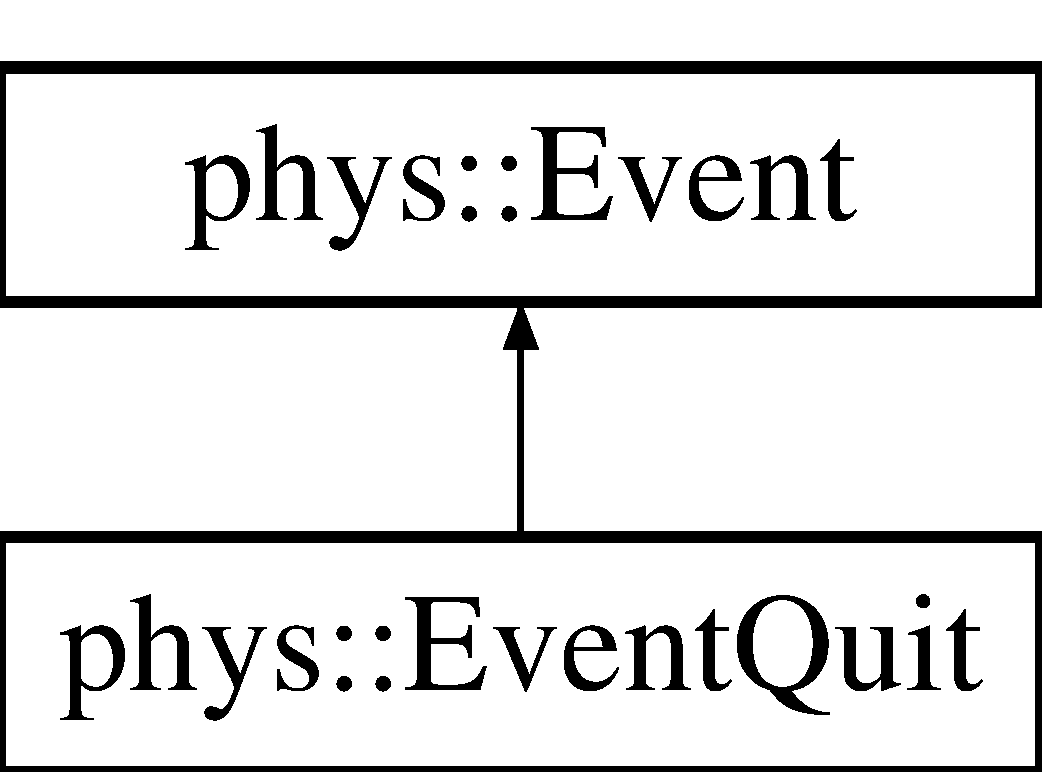
\includegraphics[height=2cm]{dd/dea/classphys_1_1EventQuit}
\end{center}
\end{figure}
\subsection*{Public Member Functions}
\begin{DoxyCompactItemize}
\item 
virtual \hyperlink{classphys_1_1EventBase_a5e6a8564e127f654123f0bf6a2751923}{EventType} \hyperlink{classphys_1_1EventQuit_a3bfca875349e73dbda47c3c62a253e3b}{GetType} () const 
\begin{DoxyCompactList}\small\item\em \hyperlink{structThis}{This} returns EventType::QuitMessage. \item\end{DoxyCompactList}\end{DoxyCompactItemize}


\subsection{Detailed Description}
\hyperlink{structThis}{This} is intended to convey the message that quitting needs to happen. \hyperlink{structThis}{This} stores not data other than the fact that this is a Quit event. \hyperlink{structThis}{This} means that either an underlying system like the OS or a service has requested a quit, or the application has manually put a quit message in the queue to signal that a graceful shutdown needs to occur. 

Definition at line 61 of file eventquit.h.



\subsection{Member Function Documentation}
\hypertarget{classphys_1_1EventQuit_a3bfca875349e73dbda47c3c62a253e3b}{
\index{phys::EventQuit@{phys::EventQuit}!GetType@{GetType}}
\index{GetType@{GetType}!phys::EventQuit@{phys::EventQuit}}
\subsubsection[{GetType}]{\setlength{\rightskip}{0pt plus 5cm}{\bf EventBase::EventType} phys::EventQuit::GetType () const\hspace{0.3cm}{\ttfamily  \mbox{[}virtual\mbox{]}}}}
\label{dd/dea/classphys_1_1EventQuit_a3bfca875349e73dbda47c3c62a253e3b}


\hyperlink{structThis}{This} returns EventType::QuitMessage. 

\hyperlink{structThis}{This} returns the kind of message this is, specifcally EventType::QuitMessage . If this functions returns EventType::QuitMessage, then and event pointer can safely be cast to \hyperlink{classphys_1_1EventQuit}{phys::EventQuit} . \hyperlink{structThis}{This} method is inherited from phys::Event . 

Implements \hyperlink{classphys_1_1EventBase_a1b3d29b6ecf30f18cc3e1825a515c508}{phys::EventBase}.



Definition at line 48 of file eventquit.cpp.



The documentation for this class was generated from the following files:\begin{DoxyCompactItemize}
\item 
eventquit.h\item 
eventquit.cpp\end{DoxyCompactItemize}

\hypertarget{classphys_1_1EventRenderTime}{
\section{phys::EventRenderTime Class Reference}
\label{d3/d8b/classphys_1_1EventRenderTime}\index{phys::EventRenderTime@{phys::EventRenderTime}}
}


This communicates the amount of time since the world was rendered.  




{\ttfamily \#include $<$eventrendertime.h$>$}

Inheritance diagram for phys::EventRenderTime:\begin{figure}[H]
\begin{center}
\leavevmode
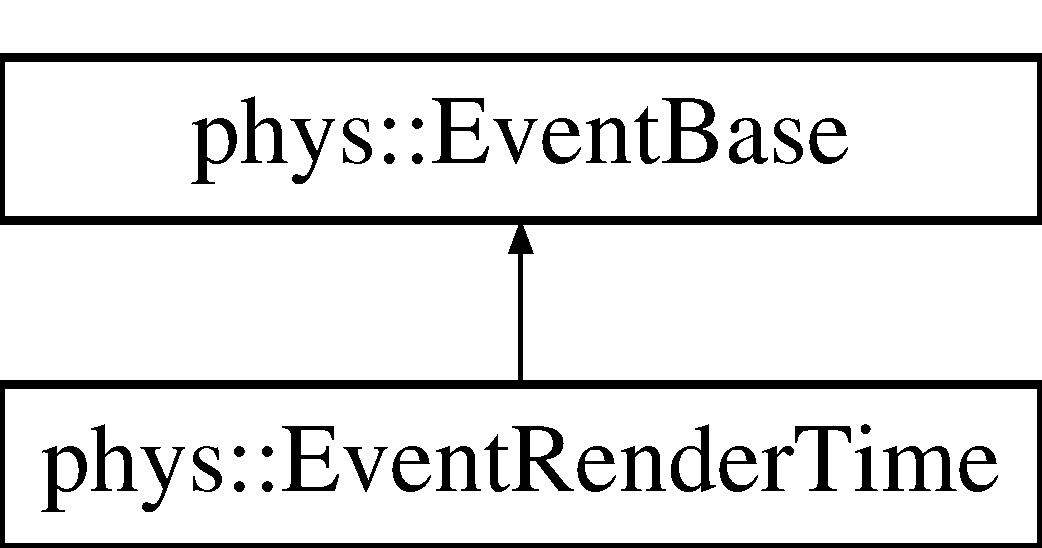
\includegraphics[height=2cm]{d3/d8b/classphys_1_1EventRenderTime}
\end{center}
\end{figure}
\subsection*{Public Member Functions}
\begin{DoxyCompactItemize}
\item 
\hyperlink{classphys_1_1EventRenderTime_af2384f7b09bbea42dcd2539a9e1747fd}{EventRenderTime} (Whole Milliseconds)
\begin{DoxyCompactList}\small\item\em The Constructor. \item\end{DoxyCompactList}\item 
virtual \hyperlink{classphys_1_1EventBase_a5e6a8564e127f654123f0bf6a2751923}{EventType} \hyperlink{classphys_1_1EventRenderTime_a76a47983d5aa197104cc3c0b9dea9dfa}{getEventType} () const 
\begin{DoxyCompactList}\small\item\em Returns that this event is a EventType::RenderTime. \item\end{DoxyCompactList}\item 
Whole \hyperlink{classphys_1_1EventRenderTime_ac9f20f13bf1f6e542151be2ce8ea2fa4}{getMilliSecondsSinceLastFrame} ()
\begin{DoxyCompactList}\small\item\em Returns the a floating point value with the amount of time. \item\end{DoxyCompactList}\end{DoxyCompactItemize}


\subsection{Detailed Description}
This communicates the amount of time since the world was rendered. This stores in milliseconds the amount of time since the last rendering of the world. 

Definition at line 59 of file eventrendertime.h.



\subsection{Constructor \& Destructor Documentation}
\hypertarget{classphys_1_1EventRenderTime_af2384f7b09bbea42dcd2539a9e1747fd}{
\index{phys::EventRenderTime@{phys::EventRenderTime}!EventRenderTime@{EventRenderTime}}
\index{EventRenderTime@{EventRenderTime}!phys::EventRenderTime@{phys::EventRenderTime}}
\subsubsection[{EventRenderTime}]{\setlength{\rightskip}{0pt plus 5cm}phys::EventRenderTime::EventRenderTime (Whole {\em Milliseconds})}}
\label{d3/d8b/classphys_1_1EventRenderTime_af2384f7b09bbea42dcd2539a9e1747fd}


The Constructor. 

This is the only way to set the time 
\begin{DoxyParams}{Parameters}
\item[{\em Milliseconds}]As it says, the amount of milliseconds since the last rendering \end{DoxyParams}


Definition at line 53 of file eventrendertime.cpp.



\subsection{Member Function Documentation}
\hypertarget{classphys_1_1EventRenderTime_a76a47983d5aa197104cc3c0b9dea9dfa}{
\index{phys::EventRenderTime@{phys::EventRenderTime}!getEventType@{getEventType}}
\index{getEventType@{getEventType}!phys::EventRenderTime@{phys::EventRenderTime}}
\subsubsection[{getEventType}]{\setlength{\rightskip}{0pt plus 5cm}{\bf EventBase::EventType} phys::EventRenderTime::getEventType () const\hspace{0.3cm}{\ttfamily  \mbox{[}virtual\mbox{]}}}}
\label{d3/d8b/classphys_1_1EventRenderTime_a76a47983d5aa197104cc3c0b9dea9dfa}


Returns that this event is a EventType::RenderTime. 

This is primarily for the benefit of sorting thorugh event pointers. If this functions returns EventType::RenderTime, then and event pointer can safely be cast to \hyperlink{classphys_1_1EventRenderTime}{phys::EventRenderTime} . This method is inherited from phys::Event . 

Implements \hyperlink{classphys_1_1EventBase_a0f39a25f4b64f7cf701e174454616366}{phys::EventBase}.



Definition at line 58 of file eventrendertime.cpp.

\hypertarget{classphys_1_1EventRenderTime_ac9f20f13bf1f6e542151be2ce8ea2fa4}{
\index{phys::EventRenderTime@{phys::EventRenderTime}!getMilliSecondsSinceLastFrame@{getMilliSecondsSinceLastFrame}}
\index{getMilliSecondsSinceLastFrame@{getMilliSecondsSinceLastFrame}!phys::EventRenderTime@{phys::EventRenderTime}}
\subsubsection[{getMilliSecondsSinceLastFrame}]{\setlength{\rightskip}{0pt plus 5cm}Whole phys::EventRenderTime::getMilliSecondsSinceLastFrame ()}}
\label{d3/d8b/classphys_1_1EventRenderTime_ac9f20f13bf1f6e542151be2ce8ea2fa4}


Returns the a floating point value with the amount of time. 

Returns the a floating point value with the amount of time. \begin{DoxyReturn}{Returns}
A floating point value with the amount of time. 
\end{DoxyReturn}


Definition at line 63 of file eventrendertime.cpp.



The documentation for this class was generated from the following files:\begin{DoxyCompactItemize}
\item 
eventrendertime.h\item 
eventrendertime.cpp\end{DoxyCompactItemize}

\hypertarget{classphys_1_1EventUserInput}{
\section{phys::EventUserInput Class Reference}
\label{d7/df5/classphys_1_1EventUserInput}\index{phys::EventUserInput@{phys::EventUserInput}}
}


This is a container for MetaCodes that is used in the physEventManager.  




{\ttfamily \#include $<$eventuserinput.h$>$}

Inheritance diagram for phys::EventUserInput:\begin{figure}[H]
\begin{center}
\leavevmode
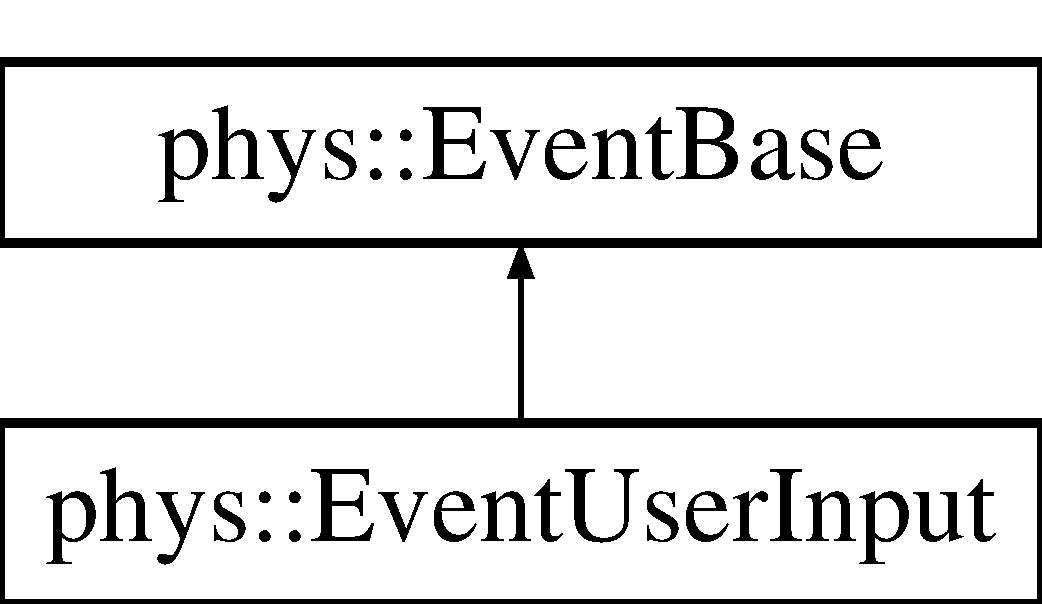
\includegraphics[height=2cm]{d7/df5/classphys_1_1EventUserInput}
\end{center}
\end{figure}
\subsection*{Public Member Functions}
\begin{DoxyCompactItemize}
\item 
\hyperlink{classphys_1_1EventUserInput_ae7358d184021306da8979000c225845e}{EventUserInput} ()
\begin{DoxyCompactList}\small\item\em Default constructor. \item\end{DoxyCompactList}\item 
\hyperlink{classphys_1_1EventUserInput_af54d4604d18b25a2dc99a4a3090b9f1d}{EventUserInput} (const \hyperlink{classphys_1_1MetaCode}{MetaCode} \&Code\_\-)
\begin{DoxyCompactList}\small\item\em Single Data Point constructor. \item\end{DoxyCompactList}\item 
\hyperlink{classphys_1_1EventUserInput_a56ca671dd5d28396cab0d7036e08a1f1}{EventUserInput} (const vector$<$ \hyperlink{classphys_1_1MetaCode}{MetaCode} $>$ \&Codes\_\-)
\begin{DoxyCompactList}\small\item\em Multi Data Point constructor. \item\end{DoxyCompactList}\item 
virtual \hyperlink{classphys_1_1EventUserInput_a5c4bb6a5016dad4cb32f51cc1d88eac3}{$\sim$EventUserInput} ()
\begin{DoxyCompactList}\small\item\em Default desstructor. \item\end{DoxyCompactList}\item 
const \hyperlink{classphys_1_1MetaCode}{MetaCode} \hyperlink{classphys_1_1EventUserInput_aaf56168b98e339cec74ae862b64632ba}{GetMetaCode} (const unsigned int \&Index)
\begin{DoxyCompactList}\small\item\em Single Data Point constructor. \item\end{DoxyCompactList}\item 
unsigned int \hyperlink{classphys_1_1EventUserInput_a17aa65dcf0ef8689affa50232eec4ccb}{GetMetaCodeCount} ()
\begin{DoxyCompactList}\small\item\em Retrieves a count of the stored Metacodes. \item\end{DoxyCompactList}\item 
void \hyperlink{classphys_1_1EventUserInput_a648f820aea2b6bca23eaa3c1e1f54181}{AddCode} (const \hyperlink{classphys_1_1MetaCode}{MetaCode} \&Code\_\-)
\begin{DoxyCompactList}\small\item\em Adds a \hyperlink{classphys_1_1MetaCode}{MetaCode}. \item\end{DoxyCompactList}\item 
void \hyperlink{classphys_1_1EventUserInput_ac9d4d8372fad7d91a5508d9e612a10e9}{AddCode} (const int \&MetaValue\_\-, const short unsigned int \&ID\_\-, const \hyperlink{classphys_1_1MetaCode_a3e501cbb5bf0f6f1fdb7211465bda8d8}{MetaCode::InputCode} \&Code\_\-)
\begin{DoxyCompactList}\small\item\em Adds a Created From Raw Values. \item\end{DoxyCompactList}\item 
void \hyperlink{classphys_1_1EventUserInput_a9b0787db5ed6e326c4932fd83798e118}{AddCode} (const \hyperlink{namespacephys_a8126d26e4507e66d09876988bb941fd4}{RawEvent} \&RawEvent\_\-)
\begin{DoxyCompactList}\small\item\em Adds a \hyperlink{classphys_1_1MetaCode}{MetaCode} created from a RawEvent. \item\end{DoxyCompactList}\item 
void \hyperlink{classphys_1_1EventUserInput_a6b6071496574fbb719ba4a5d97e74b52}{AddCode} (const vector$<$ \hyperlink{classphys_1_1MetaCode}{MetaCode} $>$ \&Codes)
\begin{DoxyCompactList}\small\item\em Add Several MetaCodes from a vector. \item\end{DoxyCompactList}\item 
void \hyperlink{classphys_1_1EventUserInput_a26a39a23deab9e54c140cc0a1cbbe6a9}{AddCodesFromRawEvent} (const \hyperlink{namespacephys_a8126d26e4507e66d09876988bb941fd4}{RawEvent} \&RawEvent\_\-)
\begin{DoxyCompactList}\small\item\em Adds all possible MetaCodes that can be created from the given RawEvent. \item\end{DoxyCompactList}\item 
void \hyperlink{classphys_1_1EventUserInput_a34c05a76a790435799441da75a83fa9c}{EraseCode} (const \hyperlink{classphys_1_1MetaCode}{MetaCode} \&Code\_\-)
\begin{DoxyCompactList}\small\item\em Removes a specific code from storage. \item\end{DoxyCompactList}\item 
void \hyperlink{classphys_1_1EventUserInput_a583084578443019d6e286b8f0e02ce58}{EraseCode} (const unsigned int \&Index)
\begin{DoxyCompactList}\small\item\em Removes a specific code from storage. \item\end{DoxyCompactList}\item 
void \hyperlink{classphys_1_1EventUserInput_adf603505c43162cf9331a486d5832f75}{ToggleCode} (const \hyperlink{classphys_1_1MetaCode}{MetaCode} \&Code\_\-)
\begin{DoxyCompactList}\small\item\em Removes a specific code or Adds it if not present. \item\end{DoxyCompactList}\item 
\hyperlink{classphys_1_1EventUserInput}{EventUserInput} \& \hyperlink{classphys_1_1EventUserInput_a1d6895e1b3814c1a63f5605b88ba85e5}{operator+=} (const \hyperlink{classphys_1_1EventUserInput}{EventUserInput} \&Add)
\begin{DoxyCompactList}\small\item\em This add all of one \hyperlink{classphys_1_1EventUserInput}{EventUserInput} to another. \item\end{DoxyCompactList}\item 
virtual \hyperlink{classphys_1_1EventBase_a5e6a8564e127f654123f0bf6a2751923}{EventType} \hyperlink{classphys_1_1EventUserInput_a3e803a8d9bcc1576fe04d2245a86ec80}{GetType} () const 
\begin{DoxyCompactList}\small\item\em Returns the type of this event. \item\end{DoxyCompactList}\end{DoxyCompactItemize}
\subsection*{Protected Attributes}
\begin{DoxyCompactItemize}
\item 
vector$<$ \hyperlink{classphys_1_1MetaCode}{MetaCode} $>$ \hyperlink{classphys_1_1EventUserInput_aee3dc1d8cac82482651487c48c6c60c9}{Code}
\begin{DoxyCompactList}\small\item\em This stores the MetaCodes in this event. \item\end{DoxyCompactList}\end{DoxyCompactItemize}


\subsection{Detailed Description}
This is a container for MetaCodes that is used in the physEventManager. The \hyperlink{classphys_1_1EventUserInput}{EventUserInput} is the container for information about how a user enters data and commands into a program. By Default one is inserted into event manager the with all the user input from the last run of the main loop. These can be manually inserted into the \hyperlink{classphys_1_1EventManager}{EventManager} to simulate input from other sources. If setup properly this can allow computer controlled characters to use the same interface players, allowing for more realistic response from them. This is not limited to the tricks discussed here. 

Definition at line 95 of file eventuserinput.h.



\subsection{Constructor \& Destructor Documentation}
\hypertarget{classphys_1_1EventUserInput_ae7358d184021306da8979000c225845e}{
\index{phys::EventUserInput@{phys::EventUserInput}!EventUserInput@{EventUserInput}}
\index{EventUserInput@{EventUserInput}!phys::EventUserInput@{phys::EventUserInput}}
\subsubsection[{EventUserInput}]{\setlength{\rightskip}{0pt plus 5cm}phys::EventUserInput::EventUserInput ()}}
\label{d7/df5/classphys_1_1EventUserInput_ae7358d184021306da8979000c225845e}


Default constructor. 

This creates a perfectly functional, but empty \hyperlink{classphys_1_1EventUserInput}{EventUserInput}. 

Definition at line 67 of file eventuserinput.cpp.

\hypertarget{classphys_1_1EventUserInput_af54d4604d18b25a2dc99a4a3090b9f1d}{
\index{phys::EventUserInput@{phys::EventUserInput}!EventUserInput@{EventUserInput}}
\index{EventUserInput@{EventUserInput}!phys::EventUserInput@{phys::EventUserInput}}
\subsubsection[{EventUserInput}]{\setlength{\rightskip}{0pt plus 5cm}phys::EventUserInput::EventUserInput (const {\bf MetaCode} \& {\em Code\_\-})}}
\label{d7/df5/classphys_1_1EventUserInput_af54d4604d18b25a2dc99a4a3090b9f1d}


Single Data Point constructor. 


\begin{DoxyParams}{Parameters}
\item[{\em Code\_\-}]This \hyperlink{classphys_1_1MetaCode}{MetaCode} will be added to the \hyperlink{classphys_1_1EventUserInput}{EventUserInput} during creation.\end{DoxyParams}
This creates a functional \hyperlink{classphys_1_1EventUserInput}{EventUserInput} which already contains one metacode. 

Definition at line 72 of file eventuserinput.cpp.

\hypertarget{classphys_1_1EventUserInput_a56ca671dd5d28396cab0d7036e08a1f1}{
\index{phys::EventUserInput@{phys::EventUserInput}!EventUserInput@{EventUserInput}}
\index{EventUserInput@{EventUserInput}!phys::EventUserInput@{phys::EventUserInput}}
\subsubsection[{EventUserInput}]{\setlength{\rightskip}{0pt plus 5cm}phys::EventUserInput::EventUserInput (const vector$<$ {\bf MetaCode} $>$ \& {\em Codes\_\-})}}
\label{d7/df5/classphys_1_1EventUserInput_a56ca671dd5d28396cab0d7036e08a1f1}


Multi Data Point constructor. 


\begin{DoxyParams}{Parameters}
\item[{\em Codes\_\-}]The MetaCodes in this vecotor will be added to the \hyperlink{classphys_1_1EventUserInput}{EventUserInput} during creation.\end{DoxyParams}
This creates a ready to use \hyperlink{classphys_1_1EventUserInput}{EventUserInput} which already contains all the metacodes included. 

Definition at line 77 of file eventuserinput.cpp.

\hypertarget{classphys_1_1EventUserInput_a5c4bb6a5016dad4cb32f51cc1d88eac3}{
\index{phys::EventUserInput@{phys::EventUserInput}!$\sim$EventUserInput@{$\sim$EventUserInput}}
\index{$\sim$EventUserInput@{$\sim$EventUserInput}!phys::EventUserInput@{phys::EventUserInput}}
\subsubsection[{$\sim$EventUserInput}]{\setlength{\rightskip}{0pt plus 5cm}phys::EventUserInput::$\sim$EventUserInput ()\hspace{0.3cm}{\ttfamily  \mbox{[}virtual\mbox{]}}}}
\label{d7/df5/classphys_1_1EventUserInput_a5c4bb6a5016dad4cb32f51cc1d88eac3}


Default desstructor. 

This tears down the 

Definition at line 82 of file eventuserinput.cpp.



\subsection{Member Function Documentation}
\hypertarget{classphys_1_1EventUserInput_a6b6071496574fbb719ba4a5d97e74b52}{
\index{phys::EventUserInput@{phys::EventUserInput}!AddCode@{AddCode}}
\index{AddCode@{AddCode}!phys::EventUserInput@{phys::EventUserInput}}
\subsubsection[{AddCode}]{\setlength{\rightskip}{0pt plus 5cm}void phys::EventUserInput::AddCode (const vector$<$ {\bf MetaCode} $>$ \& {\em Codes})}}
\label{d7/df5/classphys_1_1EventUserInput_a6b6071496574fbb719ba4a5d97e74b52}


Add Several MetaCodes from a vector. 


\begin{DoxyParams}{Parameters}
\item[{\em Codes}]A vector of MetaCodes to be added to this event\end{DoxyParams}
This adds several existing metacodes to this event. 

Definition at line 114 of file eventuserinput.cpp.

\hypertarget{classphys_1_1EventUserInput_a9b0787db5ed6e326c4932fd83798e118}{
\index{phys::EventUserInput@{phys::EventUserInput}!AddCode@{AddCode}}
\index{AddCode@{AddCode}!phys::EventUserInput@{phys::EventUserInput}}
\subsubsection[{AddCode}]{\setlength{\rightskip}{0pt plus 5cm}void phys::EventUserInput::AddCode (const {\bf RawEvent} \& {\em RawEvent\_\-})}}
\label{d7/df5/classphys_1_1EventUserInput_a9b0787db5ed6e326c4932fd83798e118}


Adds a \hyperlink{classphys_1_1MetaCode}{MetaCode} created from a RawEvent. 


\begin{DoxyParams}{Parameters}
\item[{\em RawEvent\_\-}]The RawEvent which will be translated into exactly One \hyperlink{classphys_1_1MetaCode}{MetaCode}\end{DoxyParams}
This will add \hyperlink{classphys_1_1MetaCode}{MetaCode} to this event which will be create from a RawEvent which can produce Exactly one \hyperlink{classphys_1_1MetaCode}{MetaCode}. This is used by engine internals, it is recommended to not use this in game code. \begin{DoxyWarning}{Warning}
Do not use this without reading and fully understanding the warnings on \hyperlink{classphys_1_1MetaCode_ad9a618b5cc6f9d0cf0a4bc4f47bf98e8}{MetaCode::MetaCode(const RawEvent \&RawEvent\_\-)} . This function has all the same Restrictions. If game code is using RawEvents at all, the game logic should be scrutinized carefully, it is probably wrong, but if it must it should use \hyperlink{classphys_1_1EventUserInput_a26a39a23deab9e54c140cc0a1cbbe6a9}{EventUserInput::AddCodesFromRawEvent} instead, as it can make the needed determinations automatically and in a platform agnostic way. 
\end{DoxyWarning}


Definition at line 102 of file eventuserinput.cpp.

\hypertarget{classphys_1_1EventUserInput_ac9d4d8372fad7d91a5508d9e612a10e9}{
\index{phys::EventUserInput@{phys::EventUserInput}!AddCode@{AddCode}}
\index{AddCode@{AddCode}!phys::EventUserInput@{phys::EventUserInput}}
\subsubsection[{AddCode}]{\setlength{\rightskip}{0pt plus 5cm}void phys::EventUserInput::AddCode (const int \& {\em MetaValue\_\-}, \/  const short unsigned int \& {\em ID\_\-}, \/  const {\bf MetaCode::InputCode} \& {\em Code\_\-})}}
\label{d7/df5/classphys_1_1EventUserInput_ac9d4d8372fad7d91a5508d9e612a10e9}


Adds a Created From Raw Values. 


\begin{DoxyParams}{Parameters}
\item[{\em MetaValue\_\-}]The MetaValue that will be in the \hyperlink{classphys_1_1MetaCode}{MetaCode} \item[{\em ID\_\-}]The ID that will be in the \hyperlink{classphys_1_1MetaCode}{MetaCode} \item[{\em Code\_\-}]The InputCode that will be in the \hyperlink{classphys_1_1MetaCode}{MetaCode}\end{DoxyParams}
This creates metacode a metacode and adds it to this event. 

Definition at line 108 of file eventuserinput.cpp.

\hypertarget{classphys_1_1EventUserInput_a648f820aea2b6bca23eaa3c1e1f54181}{
\index{phys::EventUserInput@{phys::EventUserInput}!AddCode@{AddCode}}
\index{AddCode@{AddCode}!phys::EventUserInput@{phys::EventUserInput}}
\subsubsection[{AddCode}]{\setlength{\rightskip}{0pt plus 5cm}void phys::EventUserInput::AddCode (const {\bf MetaCode} \& {\em Code\_\-})}}
\label{d7/df5/classphys_1_1EventUserInput_a648f820aea2b6bca23eaa3c1e1f54181}


Adds a \hyperlink{classphys_1_1MetaCode}{MetaCode}. 


\begin{DoxyParams}{Parameters}
\item[{\em Code\_\-}]The User Input \hyperlink{classphys_1_1MetaCode}{MetaCode} tobe added\end{DoxyParams}
This adds an existing metacode to this event. 

Definition at line 97 of file eventuserinput.cpp.

\hypertarget{classphys_1_1EventUserInput_a26a39a23deab9e54c140cc0a1cbbe6a9}{
\index{phys::EventUserInput@{phys::EventUserInput}!AddCodesFromRawEvent@{AddCodesFromRawEvent}}
\index{AddCodesFromRawEvent@{AddCodesFromRawEvent}!phys::EventUserInput@{phys::EventUserInput}}
\subsubsection[{AddCodesFromRawEvent}]{\setlength{\rightskip}{0pt plus 5cm}void phys::EventUserInput::AddCodesFromRawEvent (const {\bf RawEvent} \& {\em RawEvent\_\-})}}
\label{d7/df5/classphys_1_1EventUserInput_a26a39a23deab9e54c140cc0a1cbbe6a9}


Adds all possible MetaCodes that can be created from the given RawEvent. 


\begin{DoxyParams}{Parameters}
\item[{\em RawEvent\_\-}]The RawEvent which will be translated into a group of metacodes and added to this\end{DoxyParams}
This will add \hyperlink{classphys_1_1MetaCode}{MetaCode} to this event which will be create from a RawEvent which can produce Exactly one \hyperlink{classphys_1_1MetaCode}{MetaCode}. This is used by engine internals, it is recommended to not use this in game code. \begin{DoxyWarning}{Warning}
If game code is using RawEvents at all, the game logic should be scrutinized carefully, it is probably wrong, but if it must them this is the correct function to use. This will work same on a all platforms. However, the binary format of the Rawevent could chnage meaning you would have to recompile the game code to work with new version of the engine \par
 This Function is currently incomplete, and does not yet process all events such as joysticks events and some mouse events. 
\end{DoxyWarning}


Definition at line 165 of file eventuserinput.cpp.

\hypertarget{classphys_1_1EventUserInput_a583084578443019d6e286b8f0e02ce58}{
\index{phys::EventUserInput@{phys::EventUserInput}!EraseCode@{EraseCode}}
\index{EraseCode@{EraseCode}!phys::EventUserInput@{phys::EventUserInput}}
\subsubsection[{EraseCode}]{\setlength{\rightskip}{0pt plus 5cm}void phys::EventUserInput::EraseCode (const unsigned int \& {\em Index})}}
\label{d7/df5/classphys_1_1EventUserInput_a583084578443019d6e286b8f0e02ce58}


Removes a specific code from storage. 


\begin{DoxyParams}{Parameters}
\item[{\em Index}]This is the location to removed from\end{DoxyParams}
The \hyperlink{classphys_1_1MetaCode}{MetaCode} at and only at the given Index will be deleted. 

Definition at line 136 of file eventuserinput.cpp.

\hypertarget{classphys_1_1EventUserInput_a34c05a76a790435799441da75a83fa9c}{
\index{phys::EventUserInput@{phys::EventUserInput}!EraseCode@{EraseCode}}
\index{EraseCode@{EraseCode}!phys::EventUserInput@{phys::EventUserInput}}
\subsubsection[{EraseCode}]{\setlength{\rightskip}{0pt plus 5cm}void phys::EventUserInput::EraseCode (const {\bf MetaCode} \& {\em Code\_\-})}}
\label{d7/df5/classphys_1_1EventUserInput_a34c05a76a790435799441da75a83fa9c}


Removes a specific code from storage. 


\begin{DoxyParams}{Parameters}
\item[{\em Code\_\-}]This will search for all matching copies of this\end{DoxyParams}
All MetaCodes that are equal to Code\_\- will simply be erased. 

Definition at line 123 of file eventuserinput.cpp.

\hypertarget{classphys_1_1EventUserInput_aaf56168b98e339cec74ae862b64632ba}{
\index{phys::EventUserInput@{phys::EventUserInput}!GetMetaCode@{GetMetaCode}}
\index{GetMetaCode@{GetMetaCode}!phys::EventUserInput@{phys::EventUserInput}}
\subsubsection[{GetMetaCode}]{\setlength{\rightskip}{0pt plus 5cm}const {\bf MetaCode} phys::EventUserInput::GetMetaCode (const unsigned int \& {\em Index})}}
\label{d7/df5/classphys_1_1EventUserInput_aaf56168b98e339cec74ae862b64632ba}


Single Data Point constructor. 

\begin{DoxyReturn}{Returns}
Index The requested \hyperlink{classphys_1_1MetaCode}{MetaCode} to return.
\end{DoxyReturn}
This function simply retrieves the requested \hyperlink{classphys_1_1MetaCode}{MetaCode}. It can throw standard Out of bounds exceptions if attemped to reference a negative item or an item with Index higher than what exists \par
 This is useful for accessing each \hyperlink{classphys_1_1MetaCode}{MetaCode} stored in this physUserInputEvent. 

Definition at line 87 of file eventuserinput.cpp.

\hypertarget{classphys_1_1EventUserInput_a17aa65dcf0ef8689affa50232eec4ccb}{
\index{phys::EventUserInput@{phys::EventUserInput}!GetMetaCodeCount@{GetMetaCodeCount}}
\index{GetMetaCodeCount@{GetMetaCodeCount}!phys::EventUserInput@{phys::EventUserInput}}
\subsubsection[{GetMetaCodeCount}]{\setlength{\rightskip}{0pt plus 5cm}unsigned int phys::EventUserInput::GetMetaCodeCount ()}}
\label{d7/df5/classphys_1_1EventUserInput_a17aa65dcf0ef8689affa50232eec4ccb}


Retrieves a count of the stored Metacodes. 

\begin{DoxyReturn}{Returns}
The amount of codes stored in this physEventUserInput.
\end{DoxyReturn}
Retrieves a count of the stored Metacodes 

Definition at line 92 of file eventuserinput.cpp.

\hypertarget{classphys_1_1EventUserInput_a3e803a8d9bcc1576fe04d2245a86ec80}{
\index{phys::EventUserInput@{phys::EventUserInput}!GetType@{GetType}}
\index{GetType@{GetType}!phys::EventUserInput@{phys::EventUserInput}}
\subsubsection[{GetType}]{\setlength{\rightskip}{0pt plus 5cm}{\bf EventBase::EventType} phys::EventUserInput::GetType () const\hspace{0.3cm}{\ttfamily  \mbox{[}virtual\mbox{]}}}}
\label{d7/df5/classphys_1_1EventUserInput_a3e803a8d9bcc1576fe04d2245a86ec80}


Returns the type of this event. 

\begin{DoxyReturn}{Returns}
Returns EventType::UserInput 
\end{DoxyReturn}


Implements \hyperlink{classphys_1_1EventBase_a1b3d29b6ecf30f18cc3e1825a515c508}{phys::EventBase}.



Definition at line 160 of file eventuserinput.cpp.

\hypertarget{classphys_1_1EventUserInput_a1d6895e1b3814c1a63f5605b88ba85e5}{
\index{phys::EventUserInput@{phys::EventUserInput}!operator+=@{operator+=}}
\index{operator+=@{operator+=}!phys::EventUserInput@{phys::EventUserInput}}
\subsubsection[{operator+=}]{\setlength{\rightskip}{0pt plus 5cm}{\bf EventUserInput} \& phys::EventUserInput::operator+= (const {\bf EventUserInput} \& {\em Add})}}
\label{d7/df5/classphys_1_1EventUserInput_a1d6895e1b3814c1a63f5605b88ba85e5}


This add all of one \hyperlink{classphys_1_1EventUserInput}{EventUserInput} to another. 


\begin{DoxyParams}{Parameters}
\item[{\em Add}]is the \hyperlink{classphys_1_1EventUserInput}{EventUserInput} on the right hand side of +=\end{DoxyParams}
This simply copies all the MetaCodes from one \hyperlink{classphys_1_1EventUserInput}{EventUserInput} to the other. \begin{DoxyReturn}{Returns}
The \hyperlink{classphys_1_1EventUserInput}{EventUserInput} on the left ahnd side will now contain a set of both items MetaCodes 
\end{DoxyReturn}


Definition at line 198 of file eventuserinput.cpp.

\hypertarget{classphys_1_1EventUserInput_adf603505c43162cf9331a486d5832f75}{
\index{phys::EventUserInput@{phys::EventUserInput}!ToggleCode@{ToggleCode}}
\index{ToggleCode@{ToggleCode}!phys::EventUserInput@{phys::EventUserInput}}
\subsubsection[{ToggleCode}]{\setlength{\rightskip}{0pt plus 5cm}void phys::EventUserInput::ToggleCode (const {\bf MetaCode} \& {\em Code\_\-})}}
\label{d7/df5/classphys_1_1EventUserInput_adf603505c43162cf9331a486d5832f75}


Removes a specific code or Adds it if not present. 


\begin{DoxyParams}{Parameters}
\item[{\em Code\_\-}]This will search for all matching copies of this.\end{DoxyParams}
All MetaCodes that are equal to Code\_\- will simply be erased. 

Definition at line 141 of file eventuserinput.cpp.



\subsection{Member Data Documentation}
\hypertarget{classphys_1_1EventUserInput_aee3dc1d8cac82482651487c48c6c60c9}{
\index{phys::EventUserInput@{phys::EventUserInput}!Code@{Code}}
\index{Code@{Code}!phys::EventUserInput@{phys::EventUserInput}}
\subsubsection[{Code}]{\setlength{\rightskip}{0pt plus 5cm}vector$<${\bf MetaCode}$>$ {\bf phys::EventUserInput::Code}\hspace{0.3cm}{\ttfamily  \mbox{[}protected\mbox{]}}}}
\label{d7/df5/classphys_1_1EventUserInput_aee3dc1d8cac82482651487c48c6c60c9}


This stores the MetaCodes in this event. 

This stores the MetaCodes in this event. This represents a snapshot of the user input for the moment. 

Definition at line 106 of file eventuserinput.h.



The documentation for this class was generated from the following files:\begin{DoxyCompactItemize}
\item 
eventuserinput.h\item 
eventuserinput.cpp\end{DoxyCompactItemize}

\hypertarget{classphys_1_1Exception}{
\section{phys::Exception Class Reference}
\label{dc/d47/classphys_1_1Exception}\index{phys::Exception@{phys::Exception}}
}


This is the exception thrown by most physgame system that can throw exceptions.  




{\ttfamily \#include $<$exception.h$>$}

\subsection*{Public Member Functions}
\begin{DoxyCompactItemize}
\item 
\hyperlink{classphys_1_1Exception_a73fd1d2603e30f5663fef2d64df5179f}{Exception} (const \hyperlink{namespacephys_aa03900411993de7fbfec4789bc1d392e}{String} \&Message, bool Logged\_\-=false)
\begin{DoxyCompactList}\small\item\em Simple Constructor. \item\end{DoxyCompactList}\item 
virtual \hyperlink{namespacephys_aa03900411993de7fbfec4789bc1d392e}{String} \hyperlink{classphys_1_1Exception_ac929f9b3929526eec6e6b581c9a9dd73}{what} ()  throw ()
\begin{DoxyCompactList}\small\item\em Retrieves the error message. \item\end{DoxyCompactList}\item 
bool \hyperlink{classphys_1_1Exception_ab1399e25435c390db551855fda338951}{HasBeenLogged} ()
\begin{DoxyCompactList}\small\item\em Has this exception been on a trip through the Logger? \item\end{DoxyCompactList}\end{DoxyCompactItemize}


\subsection{Detailed Description}
This is the exception thrown by most physgame system that can throw exceptions. In general they work like std::exception, but also track whether they have been logged yet. 

Definition at line 57 of file exception.h.



\subsection{Constructor \& Destructor Documentation}
\hypertarget{classphys_1_1Exception_a73fd1d2603e30f5663fef2d64df5179f}{
\index{phys::Exception@{phys::Exception}!Exception@{Exception}}
\index{Exception@{Exception}!phys::Exception@{phys::Exception}}
\subsubsection[{Exception}]{\setlength{\rightskip}{0pt plus 5cm}phys::Exception::Exception (
\begin{DoxyParamCaption}
\item[{const {\bf String} \&}]{ Message, }
\item[{bool}]{ Logged\_\- = {\ttfamily false}}
\end{DoxyParamCaption}
)}}
\label{dc/d47/classphys_1_1Exception_a73fd1d2603e30f5663fef2d64df5179f}


Simple Constructor. 


\begin{DoxyParams}{Parameters}
\item[{\em Message}]The Error you want stored in the exception. \end{DoxyParams}


Definition at line 46 of file exception.cpp.



\subsection{Member Function Documentation}
\hypertarget{classphys_1_1Exception_ab1399e25435c390db551855fda338951}{
\index{phys::Exception@{phys::Exception}!HasBeenLogged@{HasBeenLogged}}
\index{HasBeenLogged@{HasBeenLogged}!phys::Exception@{phys::Exception}}
\subsubsection[{HasBeenLogged}]{\setlength{\rightskip}{0pt plus 5cm}bool phys::Exception::HasBeenLogged (
\begin{DoxyParamCaption}
{}
\end{DoxyParamCaption}
)}}
\label{dc/d47/classphys_1_1Exception_ab1399e25435c390db551855fda338951}


Has this exception been on a trip through the Logger? 

\begin{DoxyReturn}{Returns}
A bool storing true if it has and false if it has not. 
\end{DoxyReturn}


Definition at line 51 of file exception.cpp.

\hypertarget{classphys_1_1Exception_ac929f9b3929526eec6e6b581c9a9dd73}{
\index{phys::Exception@{phys::Exception}!what@{what}}
\index{what@{what}!phys::Exception@{phys::Exception}}
\subsubsection[{what}]{\setlength{\rightskip}{0pt plus 5cm}{\bf String} phys::Exception::what (
\begin{DoxyParamCaption}
{}
\end{DoxyParamCaption}
)  throw ()\hspace{0.3cm}{\ttfamily  \mbox{[}virtual\mbox{]}}}}
\label{dc/d47/classphys_1_1Exception_ac929f9b3929526eec6e6b581c9a9dd73}


Retrieves the error message. 

\begin{DoxyReturn}{Returns}
This returns a string that is the stored error message. 
\end{DoxyReturn}


Definition at line 56 of file exception.cpp.



The documentation for this class was generated from the following files:\begin{DoxyCompactItemize}
\item 
exception.h\item 
exception.cpp\end{DoxyCompactItemize}

\hypertarget{classphys_1_1Generic6DofConstraint}{
\section{phys::Generic6DofConstraint Class Reference}
\label{de/d2a/classphys_1_1Generic6DofConstraint}\index{phys::Generic6DofConstraint@{phys::Generic6DofConstraint}}
}
Inheritance diagram for phys::Generic6DofConstraint:\begin{figure}[H]
\begin{center}
\leavevmode
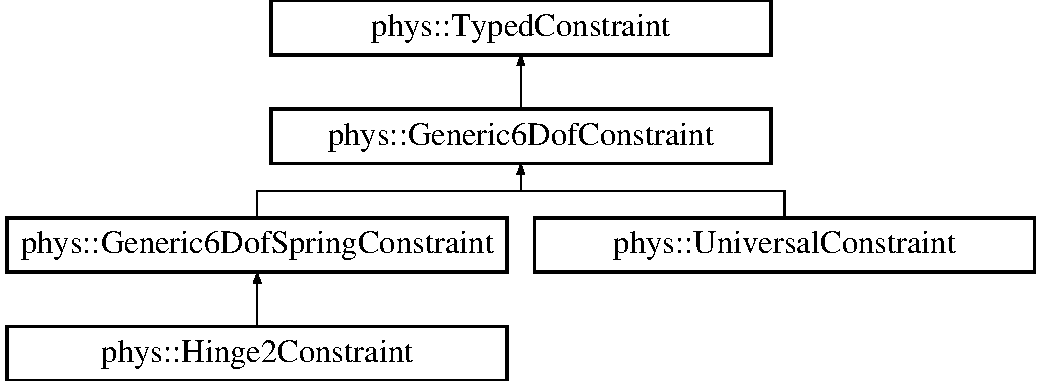
\includegraphics[height=4cm]{de/d2a/classphys_1_1Generic6DofConstraint}
\end{center}
\end{figure}
\subsection*{Public Member Functions}
\begin{DoxyCompactItemize}
\item 
\hyperlink{classphys_1_1Generic6DofConstraint_ab897b1d7f04073cae60cf1d2615d04b4}{Generic6DofConstraint} ()
\begin{DoxyCompactList}\small\item\em No initialization constructor. \item\end{DoxyCompactList}\item 
\hyperlink{classphys_1_1Generic6DofConstraint_aae8cea56ac1d384d326a089e48842cbc}{Generic6DofConstraint} (\hyperlink{classphys_1_1ActorRigid}{ActorRigid} $\ast$ActorA, \hyperlink{classphys_1_1ActorRigid}{ActorRigid} $\ast$ActorB)
\begin{DoxyCompactList}\small\item\em Inheritance constructor. \item\end{DoxyCompactList}\item 
\hypertarget{classphys_1_1Generic6DofConstraint_abcd2ccd4e4366070f6879119fe2fb985}{
{\bfseries Generic6DofConstraint} (\hyperlink{classphys_1_1ActorRigid}{ActorRigid} $\ast$ActorA, \hyperlink{classphys_1_1ActorRigid}{ActorRigid} $\ast$ActorB, \hyperlink{classphys_1_1Vector3}{Vector3} VectorA, \hyperlink{classphys_1_1Vector3}{Vector3} VectorB, \hyperlink{classphys_1_1Quaternion}{Quaternion} QuaternionA, \hyperlink{classphys_1_1Quaternion}{Quaternion} QuaternionB, bool UseLinearReferenceA)}
\label{de/d2a/classphys_1_1Generic6DofConstraint_abcd2ccd4e4366070f6879119fe2fb985}

\item 
\hypertarget{classphys_1_1Generic6DofConstraint_a4b8b1dc473a133b51d516320a10b70d5}{
{\bfseries Generic6DofConstraint} (\hyperlink{classphys_1_1ActorRigid}{ActorRigid} $\ast$ActorB, \hyperlink{classphys_1_1Vector3}{Vector3} Vectorb, \hyperlink{classphys_1_1Quaternion}{Quaternion} QuaternionB, bool UseLinearReferenceB)}
\label{de/d2a/classphys_1_1Generic6DofConstraint_a4b8b1dc473a133b51d516320a10b70d5}

\item 
\hyperlink{classphys_1_1Generic6DofConstraint_a7e44417fc8f56eb1770990fa3c3273d3}{Generic6DofConstraint} (btGeneric6DofConstraint $\ast$Constraint)
\begin{DoxyCompactList}\small\item\em Internal constructor. \item\end{DoxyCompactList}\item 
virtual \hyperlink{classphys_1_1Generic6DofConstraint_a0b0bd2e1f1546ed1e6b2ebc2a505a126}{$\sim$Generic6DofConstraint} ()
\begin{DoxyCompactList}\small\item\em Class destructor. \item\end{DoxyCompactList}\item 
\hypertarget{classphys_1_1Generic6DofConstraint_ab3897b43a2b69a91c0b11c112a79d77a}{
void {\bfseries SetOffsetALocation} (\hyperlink{classphys_1_1Vector3}{Vector3} Location)}
\label{de/d2a/classphys_1_1Generic6DofConstraint_ab3897b43a2b69a91c0b11c112a79d77a}

\item 
\hypertarget{classphys_1_1Generic6DofConstraint_ac5bee4672be646dd45274974d10ca57f}{
void {\bfseries SetOffsetBLocation} (\hyperlink{classphys_1_1Vector3}{Vector3} Location)}
\label{de/d2a/classphys_1_1Generic6DofConstraint_ac5bee4672be646dd45274974d10ca57f}

\item 
\hypertarget{classphys_1_1Generic6DofConstraint_ad6b9d20ea5a7808bb16e61e0c3ce2bac}{
void {\bfseries SetLinearUpperLimit} (\hyperlink{classphys_1_1Vector3}{Vector3} Limit)}
\label{de/d2a/classphys_1_1Generic6DofConstraint_ad6b9d20ea5a7808bb16e61e0c3ce2bac}

\item 
\hypertarget{classphys_1_1Generic6DofConstraint_a4481edd145cf461a640e9b930ffd3e98}{
void {\bfseries SetLinearLowerLimit} (\hyperlink{classphys_1_1Vector3}{Vector3} Limit)}
\label{de/d2a/classphys_1_1Generic6DofConstraint_a4481edd145cf461a640e9b930ffd3e98}

\item 
\hypertarget{classphys_1_1Generic6DofConstraint_a2a9aa0e8569335166c1d9d631279e5a4}{
void {\bfseries SetAngularUpperLimit} (\hyperlink{classphys_1_1Vector3}{Vector3} Limit)}
\label{de/d2a/classphys_1_1Generic6DofConstraint_a2a9aa0e8569335166c1d9d631279e5a4}

\item 
\hypertarget{classphys_1_1Generic6DofConstraint_a5c8799086a8cdc4a758ecf2eb6ca2c6c}{
void {\bfseries SetAngularLowerLimit} (\hyperlink{classphys_1_1Vector3}{Vector3} Limit)}
\label{de/d2a/classphys_1_1Generic6DofConstraint_a5c8799086a8cdc4a758ecf2eb6ca2c6c}

\item 
\hypertarget{classphys_1_1Generic6DofConstraint_a579b6fab2dc4897cf984c7f1a0b67210}{
void {\bfseries SetUseFrameOffset} (bool UseOffset)}
\label{de/d2a/classphys_1_1Generic6DofConstraint_a579b6fab2dc4897cf984c7f1a0b67210}

\item 
\hypertarget{classphys_1_1Generic6DofConstraint_afbf5173d41f31dda693c3591b72adf1c}{
void {\bfseries SetLimit} (int Axis, \hyperlink{namespacephys_af7eb897198d265b8e868f45240230d5f}{Real} Low, \hyperlink{namespacephys_af7eb897198d265b8e868f45240230d5f}{Real} High)}
\label{de/d2a/classphys_1_1Generic6DofConstraint_afbf5173d41f31dda693c3591b72adf1c}

\item 
\hypertarget{classphys_1_1Generic6DofConstraint_ab954137222c74dbe2d4410738b3f6883}{
void {\bfseries CalculateTransforms} ()}
\label{de/d2a/classphys_1_1Generic6DofConstraint_ab954137222c74dbe2d4410738b3f6883}

\item 
\hypertarget{classphys_1_1Generic6DofConstraint_a644245f0533a2fe1586609fcf1f48171}{
virtual void {\bfseries SetParam} (int num, \hyperlink{namespacephys_af7eb897198d265b8e868f45240230d5f}{Real} value, int axis=-\/1)}
\label{de/d2a/classphys_1_1Generic6DofConstraint_a644245f0533a2fe1586609fcf1f48171}

\item 
\hypertarget{classphys_1_1Generic6DofConstraint_a822152201f9bd6d0a3e1512fa25b3f49}{
virtual \hyperlink{namespacephys_af7eb897198d265b8e868f45240230d5f}{Real} {\bfseries GetParam} (int num, int axis=-\/1)}
\label{de/d2a/classphys_1_1Generic6DofConstraint_a822152201f9bd6d0a3e1512fa25b3f49}

\end{DoxyCompactItemize}
\subsection*{Protected Attributes}
\begin{DoxyCompactItemize}
\item 
\hypertarget{classphys_1_1Generic6DofConstraint_af323a51e2e4438fc86af1f10a84cc1ba}{
btGeneric6DofConstraint $\ast$ \hyperlink{classphys_1_1Generic6DofConstraint_af323a51e2e4438fc86af1f10a84cc1ba}{Generic6dof}}
\label{de/d2a/classphys_1_1Generic6DofConstraint_af323a51e2e4438fc86af1f10a84cc1ba}

\begin{DoxyCompactList}\small\item\em Bullet constraint that this class encapsulates. \item\end{DoxyCompactList}\end{DoxyCompactItemize}


\subsection{Detailed Description}


Definition at line 133 of file constraint.h.



\subsection{Constructor \& Destructor Documentation}
\hypertarget{classphys_1_1Generic6DofConstraint_ab897b1d7f04073cae60cf1d2615d04b4}{
\index{phys::Generic6DofConstraint@{phys::Generic6DofConstraint}!Generic6DofConstraint@{Generic6DofConstraint}}
\index{Generic6DofConstraint@{Generic6DofConstraint}!phys::Generic6DofConstraint@{phys::Generic6DofConstraint}}
\subsubsection[{Generic6DofConstraint}]{\setlength{\rightskip}{0pt plus 5cm}phys::Generic6DofConstraint::Generic6DofConstraint ()}}
\label{de/d2a/classphys_1_1Generic6DofConstraint_ab897b1d7f04073cae60cf1d2615d04b4}


No initialization constructor. 

The no initialization class constructor. 

Definition at line 172 of file constraint.cpp.

\hypertarget{classphys_1_1Generic6DofConstraint_aae8cea56ac1d384d326a089e48842cbc}{
\index{phys::Generic6DofConstraint@{phys::Generic6DofConstraint}!Generic6DofConstraint@{Generic6DofConstraint}}
\index{Generic6DofConstraint@{Generic6DofConstraint}!phys::Generic6DofConstraint@{phys::Generic6DofConstraint}}
\subsubsection[{Generic6DofConstraint}]{\setlength{\rightskip}{0pt plus 5cm}phys::Generic6DofConstraint::Generic6DofConstraint ({\bf ActorRigid} $\ast$ {\em ActorA}, \/  {\bf ActorRigid} $\ast$ {\em ActorB})}}
\label{de/d2a/classphys_1_1Generic6DofConstraint_aae8cea56ac1d384d326a089e48842cbc}


Inheritance constructor. 

This constructor exists for passing values down the inheritance tree from derived classes. Should not be called on manually. 
\begin{DoxyParams}{Parameters}
\item[{\em ActorA}]First actor to have the constraint applied to. \item[{\em ActorB}]Second actor to have the constraint applied to. \end{DoxyParams}


Definition at line 176 of file constraint.cpp.

\hypertarget{classphys_1_1Generic6DofConstraint_a7e44417fc8f56eb1770990fa3c3273d3}{
\index{phys::Generic6DofConstraint@{phys::Generic6DofConstraint}!Generic6DofConstraint@{Generic6DofConstraint}}
\index{Generic6DofConstraint@{Generic6DofConstraint}!phys::Generic6DofConstraint@{phys::Generic6DofConstraint}}
\subsubsection[{Generic6DofConstraint}]{\setlength{\rightskip}{0pt plus 5cm}phys::Generic6DofConstraint::Generic6DofConstraint (btGeneric6DofConstraint $\ast$ {\em Constraint})}}
\label{de/d2a/classphys_1_1Generic6DofConstraint_a7e44417fc8f56eb1770990fa3c3273d3}


Internal constructor. 

Constructs this class around a pre-\/built bullet constraint. This is an internal only constructor and shouldn't be called manually. 
\begin{DoxyParams}{Parameters}
\item[{\em Constraint}]The constraint to be constructed around. \end{DoxyParams}


Definition at line 196 of file constraint.cpp.

\hypertarget{classphys_1_1Generic6DofConstraint_a0b0bd2e1f1546ed1e6b2ebc2a505a126}{
\index{phys::Generic6DofConstraint@{phys::Generic6DofConstraint}!$\sim$Generic6DofConstraint@{$\sim$Generic6DofConstraint}}
\index{$\sim$Generic6DofConstraint@{$\sim$Generic6DofConstraint}!phys::Generic6DofConstraint@{phys::Generic6DofConstraint}}
\subsubsection[{$\sim$Generic6DofConstraint}]{\setlength{\rightskip}{0pt plus 5cm}phys::Generic6DofConstraint::$\sim$Generic6DofConstraint ()\hspace{0.3cm}{\ttfamily  \mbox{[}virtual\mbox{]}}}}
\label{de/d2a/classphys_1_1Generic6DofConstraint_a0b0bd2e1f1546ed1e6b2ebc2a505a126}


Class destructor. 

The class destructor. 

Definition at line 202 of file constraint.cpp.



The documentation for this class was generated from the following files:\begin{DoxyCompactItemize}
\item 
constraint.h\item 
constraint.cpp\end{DoxyCompactItemize}

\hypertarget{classphys_1_1Generic6DofSpringConstraint}{
\subsection{phys::Generic6DofSpringConstraint Class Reference}
\label{classphys_1_1Generic6DofSpringConstraint}\index{phys::Generic6DofSpringConstraint@{phys::Generic6DofSpringConstraint}}
}


Creates a constraint as configurable as the 6Dof constraint, but has added support for spring motion.  




{\ttfamily \#include $<$constraint.h$>$}

Inheritance diagram for phys::Generic6DofSpringConstraint:\begin{figure}[H]
\begin{center}
\leavevmode
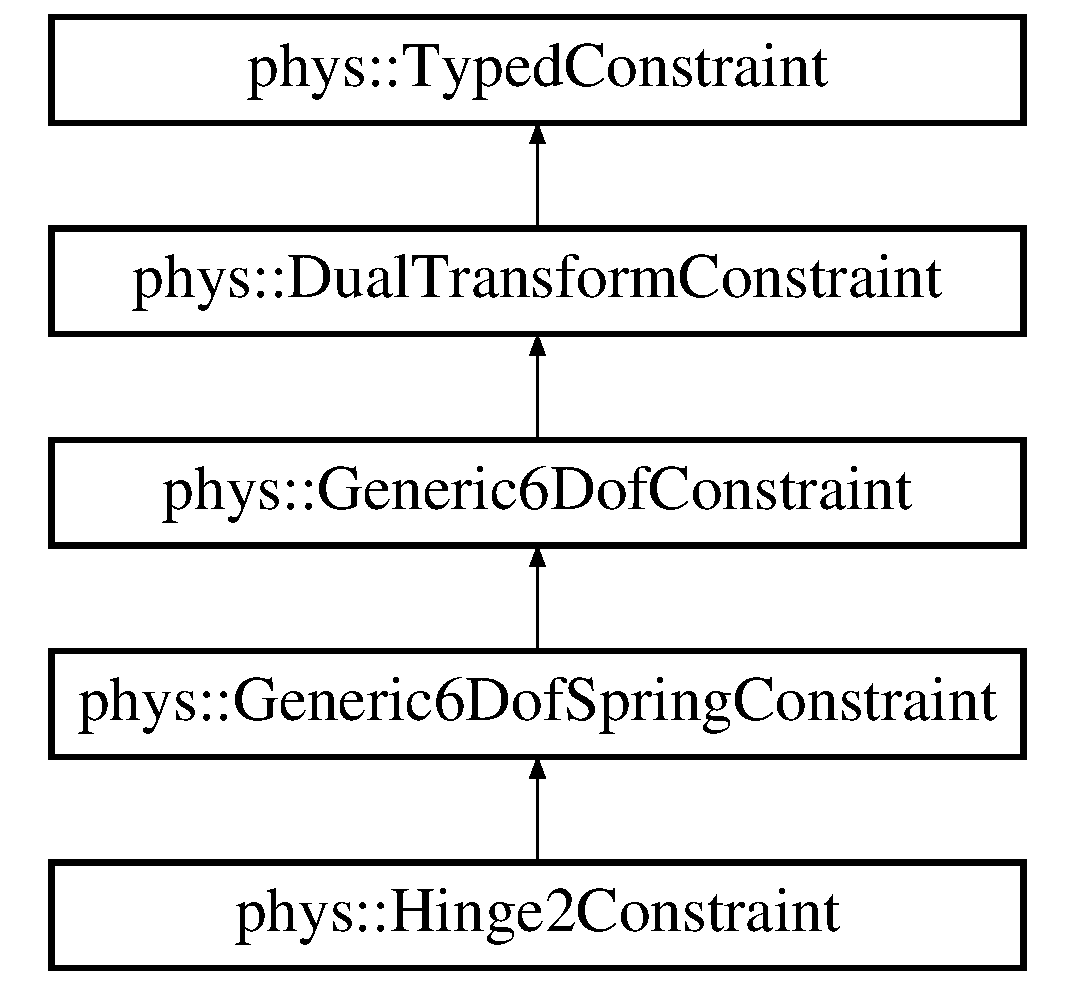
\includegraphics[height=5.000000cm]{classphys_1_1Generic6DofSpringConstraint}
\end{center}
\end{figure}
\subsubsection*{Public Types}
\begin{DoxyCompactItemize}
\item 
enum \hyperlink{classphys_1_1Generic6DofSpringConstraint_a525a9ce88c6160c44be748fe45833f60}{UsableAxis} \{ \par
\hyperlink{classphys_1_1Generic6DofSpringConstraint_a525a9ce88c6160c44be748fe45833f60afec9af16b6403edd5b6a335edbe9bffa}{LinearX} =  0, 
\hyperlink{classphys_1_1Generic6DofSpringConstraint_a525a9ce88c6160c44be748fe45833f60a243508b551645b17b8e5c42a1cf9fb72}{LinearY} =  1, 
\hyperlink{classphys_1_1Generic6DofSpringConstraint_a525a9ce88c6160c44be748fe45833f60a9d809c690118d2a37481e7aa83422492}{LinearZ} =  2, 
\hyperlink{classphys_1_1Generic6DofSpringConstraint_a525a9ce88c6160c44be748fe45833f60a52103c17e319667035ba2194f951a7d0}{AngularX} =  3, 
\par
\hyperlink{classphys_1_1Generic6DofSpringConstraint_a525a9ce88c6160c44be748fe45833f60a009951290fedb86fc9278868f7638593}{AngularY} =  4, 
\hyperlink{classphys_1_1Generic6DofSpringConstraint_a525a9ce88c6160c44be748fe45833f60a2e8e892005c4f63f43f2b42fa73c743b}{AngularZ} =  5
 \}
\begin{DoxyCompactList}\small\item\em Identify the Axis a bit easier when iterating over them is less convienent than typing an Identifier. \item\end{DoxyCompactList}\end{DoxyCompactItemize}
\subsubsection*{Public Member Functions}
\begin{DoxyCompactItemize}
\item 
\hypertarget{classphys_1_1Generic6DofSpringConstraint_aaec332a131a3e17c19c96a8ce29c9fae}{
virtual void {\bfseries CalculateSpringEquilibriumPoint} ()}
\label{classphys_1_1Generic6DofSpringConstraint_aaec332a131a3e17c19c96a8ce29c9fae}

\item 
\hypertarget{classphys_1_1Generic6DofSpringConstraint_ad1bab377a08cc0d42dd3135779611f4a}{
virtual void {\bfseries CalculateSpringEquilibriumPoint} (int Index)}
\label{classphys_1_1Generic6DofSpringConstraint_ad1bab377a08cc0d42dd3135779611f4a}

\item 
\hyperlink{classphys_1_1Generic6DofSpringConstraint_a826580505965216b75ea41f26e2ad92f}{Generic6DofSpringConstraint} (\hyperlink{classphys_1_1ActorRigid}{ActorRigid} $\ast$ActorA, \hyperlink{classphys_1_1ActorRigid}{ActorRigid} $\ast$ActorB, const \hyperlink{classphys_1_1Vector3}{Vector3} \&VectorA, const \hyperlink{classphys_1_1Vector3}{Vector3} \&VectorB, const \hyperlink{classphys_1_1Quaternion}{Quaternion} \&QuaternionA, const \hyperlink{classphys_1_1Quaternion}{Quaternion} \&QuaternionB, bool UseLinearReferenceA=false)
\begin{DoxyCompactList}\small\item\em Two body Verbose constructor. \item\end{DoxyCompactList}\item 
\hyperlink{classphys_1_1Generic6DofSpringConstraint_adb6c637cc1b18344c3c3e6cfe10dbd49}{Generic6DofSpringConstraint} (\hyperlink{classphys_1_1ActorRigid}{ActorRigid} $\ast$ActorA, \hyperlink{classphys_1_1ActorRigid}{ActorRigid} $\ast$ActorB, const \hyperlink{classphys_1_1Transform}{Transform} \&TransformA, const \hyperlink{classphys_1_1Transform}{Transform} \&TransformB, bool UseLinearReferenceA=false)
\begin{DoxyCompactList}\small\item\em Two body Terse constructor. \item\end{DoxyCompactList}\item 
\hypertarget{classphys_1_1Generic6DofSpringConstraint_a87c90750b655ae7f9f1616a660062cf1}{
virtual \hyperlink{classphys_1_1Vector3}{Vector3} {\bfseries GetCurrentSpringAngularEquilibriumPoints} () const }
\label{classphys_1_1Generic6DofSpringConstraint_a87c90750b655ae7f9f1616a660062cf1}

\item 
\hypertarget{classphys_1_1Generic6DofSpringConstraint_ad33276f69fc1768d430cd10c1b08b575}{
virtual \hyperlink{namespacephys_af7eb897198d265b8e868f45240230d5f}{Real} {\bfseries GetCurrentSpringEquilibriumPoint} (int Index) const }
\label{classphys_1_1Generic6DofSpringConstraint_ad33276f69fc1768d430cd10c1b08b575}

\item 
\hypertarget{classphys_1_1Generic6DofSpringConstraint_af4e520edbe0c5f40fac000adc5a8ad54}{
virtual \hyperlink{classphys_1_1Vector3}{Vector3} {\bfseries GetCurrentSpringLinearEquilibriumPoints} () const }
\label{classphys_1_1Generic6DofSpringConstraint_af4e520edbe0c5f40fac000adc5a8ad54}

\item 
virtual \hyperlink{classphys_1_1Vector3}{Vector3} \hyperlink{classphys_1_1Generic6DofSpringConstraint_a7b8a8733b7a8d25c0d84684a69624334}{GetSpringAngularDamping} () const 
\begin{DoxyCompactList}\small\item\em Get the Damping for all Angular Axis. \item\end{DoxyCompactList}\item 
virtual \hyperlink{classphys_1_1Vector3}{Vector3} \hyperlink{classphys_1_1Generic6DofSpringConstraint_a3aac6b13a8127ba82354f436c624c879}{GetSpringAngularEnabled} () const 
\begin{DoxyCompactList}\small\item\em Get the Enabled Status for all Angular Axis. \item\end{DoxyCompactList}\item 
virtual \hyperlink{classphys_1_1Vector3}{Vector3} \hyperlink{classphys_1_1Generic6DofSpringConstraint_a8e51c0141b190a4c34365abc9dc11a98}{GetSpringAngularStiffness} () const 
\begin{DoxyCompactList}\small\item\em Get the Stiffness for all Angular Axis. \item\end{DoxyCompactList}\item 
virtual \hyperlink{namespacephys_af7eb897198d265b8e868f45240230d5f}{Real} \hyperlink{classphys_1_1Generic6DofSpringConstraint_a662d116e3467851e9d6bba6b01d3382a}{GetSpringDamping} (int Index) const 
\begin{DoxyCompactList}\small\item\em Retrieve the Damping of the spring on the given axis. \item\end{DoxyCompactList}\item 
virtual bool \hyperlink{classphys_1_1Generic6DofSpringConstraint_a921afe66b38b967e666c53a8448d4a00}{GetSpringEnabled} (int Index) const 
\begin{DoxyCompactList}\small\item\em Retrieve the EnabledStatus of the spring on the given axis. \item\end{DoxyCompactList}\item 
virtual \hyperlink{classphys_1_1Vector3}{Vector3} \hyperlink{classphys_1_1Generic6DofSpringConstraint_ab58b5111016f4f29343b0097848de2d2}{GetSpringLinearDamping} () const 
\begin{DoxyCompactList}\small\item\em Get the Damping for all Linear Axis. \item\end{DoxyCompactList}\item 
virtual \hyperlink{classphys_1_1Vector3}{Vector3} \hyperlink{classphys_1_1Generic6DofSpringConstraint_abc9670d0ca5631994b0e260428ee1110}{GetSpringLinearEnabled} () const 
\begin{DoxyCompactList}\small\item\em Get the Enabled Status for all Linear Axis. \item\end{DoxyCompactList}\item 
virtual \hyperlink{classphys_1_1Vector3}{Vector3} \hyperlink{classphys_1_1Generic6DofSpringConstraint_a2ef04c27d4340bb41233129e387b1145}{GetSpringLinearStiffness} () const 
\begin{DoxyCompactList}\small\item\em Get the Stiffness for all Linear Axis. \item\end{DoxyCompactList}\item 
virtual \hyperlink{namespacephys_af7eb897198d265b8e868f45240230d5f}{Real} \hyperlink{classphys_1_1Generic6DofSpringConstraint_a06d43edcb68aa820060a60b49387f9e6}{GetSpringStiffness} (int Index) const 
\begin{DoxyCompactList}\small\item\em Retrieve the Stiffness of the spring on the given axis. \item\end{DoxyCompactList}\item 
virtual void \hyperlink{classphys_1_1Generic6DofSpringConstraint_aa92969027509290efc128334b01db500}{ProtoDeSerialize} (const \hyperlink{classphys_1_1xml_1_1Node}{xml::Node} \&OneNode)
\begin{DoxyCompactList}\small\item\em Take the data stored in an XML and overwrite this instance of this object with it. \item\end{DoxyCompactList}\item 
virtual void \hyperlink{classphys_1_1Generic6DofSpringConstraint_aeffb182d5faa82175e96a259fc19f9ff}{ProtoSerialize} (\hyperlink{classphys_1_1xml_1_1Node}{xml::Node} \&CurrentRoot) const 
\begin{DoxyCompactList}\small\item\em Convert this class to an \hyperlink{classphys_1_1xml_1_1Node}{xml::Node} ready for serialization. \item\end{DoxyCompactList}\item 
\hyperlink{namespacephys_aa03900411993de7fbfec4789bc1d392e}{String} \hyperlink{classphys_1_1Generic6DofSpringConstraint_ad0a2d0c49fb622095f18d48b1e52f904}{SerializableName} () const 
\begin{DoxyCompactList}\small\item\em Get the name of the the XML tag this class will leave behind as its instances are serialized. \item\end{DoxyCompactList}\item 
virtual void \hyperlink{classphys_1_1Generic6DofSpringConstraint_a65dbf1070a4277dd0d27e48db2b45c89}{SetSpringAngularDamping} (const \hyperlink{classphys_1_1Vector3}{Vector3} \&Damps)
\begin{DoxyCompactList}\small\item\em Set the Damping of the springs on each Angular Axis. \item\end{DoxyCompactList}\item 
virtual void \hyperlink{classphys_1_1Generic6DofSpringConstraint_a1f861c64cc9d4918bd3dbe606894422e}{SetSpringAngularEnabled} (const \hyperlink{classphys_1_1Vector3}{Vector3} \&Enableness)
\begin{DoxyCompactList}\small\item\em Set the Stiffness of the springs on each Angular Axis. \item\end{DoxyCompactList}\item 
virtual void \hyperlink{classphys_1_1Generic6DofSpringConstraint_ab1d57e737c3471acd9a9481abb9ac612}{SetSpringAngularStiffness} (const \hyperlink{classphys_1_1Vector3}{Vector3} \&Stiffies)
\begin{DoxyCompactList}\small\item\em Set the Stiffness of the springs on each Angular Axis. \item\end{DoxyCompactList}\item 
virtual void \hyperlink{classphys_1_1Generic6DofSpringConstraint_a5e39d3b9601b1d8ec6e3197b1cc999a7}{SetSpringDamping} (int Index, \hyperlink{namespacephys_af7eb897198d265b8e868f45240230d5f}{Real} Damping)
\begin{DoxyCompactList}\small\item\em Set the spring Damping on a given axis. \item\end{DoxyCompactList}\item 
virtual void \hyperlink{classphys_1_1Generic6DofSpringConstraint_a49ab6cbd0859e455391b1b676b1309b7}{SetSpringEnabled} (int Index, bool Enable)
\begin{DoxyCompactList}\small\item\em Set the spring's enabled status on a given axis. \item\end{DoxyCompactList}\item 
virtual void \hyperlink{classphys_1_1Generic6DofSpringConstraint_a86776512ae4f20d4143aa4c8901ab355}{SetSpringLinearDamping} (const \hyperlink{classphys_1_1Vector3}{Vector3} \&Damps)
\begin{DoxyCompactList}\small\item\em Set the Damping of the springs on each Linear Axis. \item\end{DoxyCompactList}\item 
virtual void \hyperlink{classphys_1_1Generic6DofSpringConstraint_a561603d0470dc20eb74ee79cc1131c52}{SetSpringLinearEnabled} (const \hyperlink{classphys_1_1Vector3}{Vector3} \&Enableness)
\begin{DoxyCompactList}\small\item\em Set the Stiffness of the springs on each Linear Axis. \item\end{DoxyCompactList}\item 
virtual void \hyperlink{classphys_1_1Generic6DofSpringConstraint_a3cb5c0a8cfacc634728828eb85b2b025}{SetSpringLinearStiffness} (const \hyperlink{classphys_1_1Vector3}{Vector3} \&Stiffies)
\begin{DoxyCompactList}\small\item\em Set the Stiffness of the springs on each Linear Axis. \item\end{DoxyCompactList}\item 
virtual void \hyperlink{classphys_1_1Generic6DofSpringConstraint_a7a73106f73e23320cc84593aade54301}{SetSpringStiffness} (int Index, \hyperlink{namespacephys_af7eb897198d265b8e868f45240230d5f}{Real} Stiffness)
\begin{DoxyCompactList}\small\item\em Set the spring stiffness on a given axis. \item\end{DoxyCompactList}\item 
virtual \hyperlink{classphys_1_1Generic6DofSpringConstraint_a66a886a64c86a24ed34eacf4c8465f10}{$\sim$Generic6DofSpringConstraint} ()
\begin{DoxyCompactList}\small\item\em Class destructor. \item\end{DoxyCompactList}\end{DoxyCompactItemize}
\subsubsection*{Protected Member Functions}
\begin{DoxyCompactItemize}
\item 
virtual btGeneric6DofSpringConstraint $\ast$ \hyperlink{classphys_1_1Generic6DofSpringConstraint_a9b8621e2f9cd34fe183de6e664959027}{Generic6dofSpring} () const 
\item 
\hyperlink{classphys_1_1Generic6DofSpringConstraint_aeca02121a3d7d2416a611c2f7274c1a6}{Generic6DofSpringConstraint} ()
\begin{DoxyCompactList}\small\item\em Inheritance Constructor. \item\end{DoxyCompactList}\end{DoxyCompactItemize}


\subsubsection{Detailed Description}
Creates a constraint as configurable as the 6Dof constraint, but has added support for spring motion. When using functions of this class that require you to specify the index, the springs are arranged like so: \par

\begin{DoxyItemize}
\item 0: Translation X
\item 1: Translation Y
\item 2: Translation Z
\item 3: Rotation X
\item 4: Rotation Y
\item 5: Rotation Z 
\end{DoxyItemize}

Definition at line 814 of file constraint.h.



\subsubsection{Member Enumeration Documentation}
\hypertarget{classphys_1_1Generic6DofSpringConstraint_a525a9ce88c6160c44be748fe45833f60}{
\index{phys::Generic6DofSpringConstraint@{phys::Generic6DofSpringConstraint}!UsableAxis@{UsableAxis}}
\index{UsableAxis@{UsableAxis}!phys::Generic6DofSpringConstraint@{phys::Generic6DofSpringConstraint}}
\paragraph[{UsableAxis}]{\setlength{\rightskip}{0pt plus 5cm}enum {\bf phys::Generic6DofSpringConstraint::UsableAxis}}\hfill}
\label{classphys_1_1Generic6DofSpringConstraint_a525a9ce88c6160c44be748fe45833f60}


Identify the Axis a bit easier when iterating over them is less convienent than typing an Identifier. 

\begin{Desc}
\item[Enumerator: ]\par
\begin{description}
\index{LinearX@{LinearX}!phys::Generic6DofSpringConstraint@{phys::Generic6DofSpringConstraint}}\index{phys::Generic6DofSpringConstraint@{phys::Generic6DofSpringConstraint}!LinearX@{LinearX}}\item[{\em 
\hypertarget{classphys_1_1Generic6DofSpringConstraint_a525a9ce88c6160c44be748fe45833f60afec9af16b6403edd5b6a335edbe9bffa}{
LinearX}
\label{classphys_1_1Generic6DofSpringConstraint_a525a9ce88c6160c44be748fe45833f60afec9af16b6403edd5b6a335edbe9bffa}
}]Translation on the X axis. \index{LinearY@{LinearY}!phys::Generic6DofSpringConstraint@{phys::Generic6DofSpringConstraint}}\index{phys::Generic6DofSpringConstraint@{phys::Generic6DofSpringConstraint}!LinearY@{LinearY}}\item[{\em 
\hypertarget{classphys_1_1Generic6DofSpringConstraint_a525a9ce88c6160c44be748fe45833f60a243508b551645b17b8e5c42a1cf9fb72}{
LinearY}
\label{classphys_1_1Generic6DofSpringConstraint_a525a9ce88c6160c44be748fe45833f60a243508b551645b17b8e5c42a1cf9fb72}
}]Translation on the Y axis. \index{LinearZ@{LinearZ}!phys::Generic6DofSpringConstraint@{phys::Generic6DofSpringConstraint}}\index{phys::Generic6DofSpringConstraint@{phys::Generic6DofSpringConstraint}!LinearZ@{LinearZ}}\item[{\em 
\hypertarget{classphys_1_1Generic6DofSpringConstraint_a525a9ce88c6160c44be748fe45833f60a9d809c690118d2a37481e7aa83422492}{
LinearZ}
\label{classphys_1_1Generic6DofSpringConstraint_a525a9ce88c6160c44be748fe45833f60a9d809c690118d2a37481e7aa83422492}
}]Translation on the Z axis. \index{AngularX@{AngularX}!phys::Generic6DofSpringConstraint@{phys::Generic6DofSpringConstraint}}\index{phys::Generic6DofSpringConstraint@{phys::Generic6DofSpringConstraint}!AngularX@{AngularX}}\item[{\em 
\hypertarget{classphys_1_1Generic6DofSpringConstraint_a525a9ce88c6160c44be748fe45833f60a52103c17e319667035ba2194f951a7d0}{
AngularX}
\label{classphys_1_1Generic6DofSpringConstraint_a525a9ce88c6160c44be748fe45833f60a52103c17e319667035ba2194f951a7d0}
}]Rotation on the X axis. \index{AngularY@{AngularY}!phys::Generic6DofSpringConstraint@{phys::Generic6DofSpringConstraint}}\index{phys::Generic6DofSpringConstraint@{phys::Generic6DofSpringConstraint}!AngularY@{AngularY}}\item[{\em 
\hypertarget{classphys_1_1Generic6DofSpringConstraint_a525a9ce88c6160c44be748fe45833f60a009951290fedb86fc9278868f7638593}{
AngularY}
\label{classphys_1_1Generic6DofSpringConstraint_a525a9ce88c6160c44be748fe45833f60a009951290fedb86fc9278868f7638593}
}]Rotation on the Y axis. \index{AngularZ@{AngularZ}!phys::Generic6DofSpringConstraint@{phys::Generic6DofSpringConstraint}}\index{phys::Generic6DofSpringConstraint@{phys::Generic6DofSpringConstraint}!AngularZ@{AngularZ}}\item[{\em 
\hypertarget{classphys_1_1Generic6DofSpringConstraint_a525a9ce88c6160c44be748fe45833f60a2e8e892005c4f63f43f2b42fa73c743b}{
AngularZ}
\label{classphys_1_1Generic6DofSpringConstraint_a525a9ce88c6160c44be748fe45833f60a2e8e892005c4f63f43f2b42fa73c743b}
}]Rotation on the Z axis. \end{description}
\end{Desc}



Reimplemented from \hyperlink{classphys_1_1Generic6DofConstraint_a70c7ba15366ae33deaf8e042b32f8e02}{phys::Generic6DofConstraint}.



Definition at line 824 of file constraint.h.



\subsubsection{Constructor \& Destructor Documentation}
\hypertarget{classphys_1_1Generic6DofSpringConstraint_aeca02121a3d7d2416a611c2f7274c1a6}{
\index{phys::Generic6DofSpringConstraint@{phys::Generic6DofSpringConstraint}!Generic6DofSpringConstraint@{Generic6DofSpringConstraint}}
\index{Generic6DofSpringConstraint@{Generic6DofSpringConstraint}!phys::Generic6DofSpringConstraint@{phys::Generic6DofSpringConstraint}}
\paragraph[{Generic6DofSpringConstraint}]{\setlength{\rightskip}{0pt plus 5cm}phys::Generic6DofSpringConstraint::Generic6DofSpringConstraint (
\begin{DoxyParamCaption}
{}
\end{DoxyParamCaption}
)\hspace{0.3cm}{\ttfamily  \mbox{[}protected\mbox{]}}}\hfill}
\label{classphys_1_1Generic6DofSpringConstraint_aeca02121a3d7d2416a611c2f7274c1a6}


Inheritance Constructor. 

This is only called by derived classes, and shouldn't be called manually. \hypertarget{classphys_1_1Generic6DofSpringConstraint_a826580505965216b75ea41f26e2ad92f}{
\index{phys::Generic6DofSpringConstraint@{phys::Generic6DofSpringConstraint}!Generic6DofSpringConstraint@{Generic6DofSpringConstraint}}
\index{Generic6DofSpringConstraint@{Generic6DofSpringConstraint}!phys::Generic6DofSpringConstraint@{phys::Generic6DofSpringConstraint}}
\paragraph[{Generic6DofSpringConstraint}]{\setlength{\rightskip}{0pt plus 5cm}phys::Generic6DofSpringConstraint::Generic6DofSpringConstraint (
\begin{DoxyParamCaption}
\item[{{\bf ActorRigid} $\ast$}]{ActorA, }
\item[{{\bf ActorRigid} $\ast$}]{ActorB, }
\item[{const {\bf Vector3} \&}]{VectorA, }
\item[{const {\bf Vector3} \&}]{VectorB, }
\item[{const {\bf Quaternion} \&}]{QuaternionA, }
\item[{const {\bf Quaternion} \&}]{QuaternionB, }
\item[{bool}]{UseLinearReferenceA = {\ttfamily false}}
\end{DoxyParamCaption}
)}\hfill}
\label{classphys_1_1Generic6DofSpringConstraint_a826580505965216b75ea41f26e2ad92f}


Two body Verbose constructor. 


\begin{DoxyParams}{Parameters}
{\em ActorA} & The First body to be bound \\
\hline
{\em ActorB} & The Second body to be bound \\
\hline
{\em VectorA} & The offset from ActorA's center of gravity to get to match an offset from ActorB \\
\hline
{\em VectorB} & The offset from ActorB's center of gravity. \\
\hline
{\em QuaternionA} & Relative rotation from ActorA \\
\hline
{\em QuaternionB} & Relative rotation from ActorB \\
\hline
{\em UseLinearReferenceA} & Perform Linear math from ActorA's perspective, default to false. \\
\hline
\end{DoxyParams}
\hypertarget{classphys_1_1Generic6DofSpringConstraint_adb6c637cc1b18344c3c3e6cfe10dbd49}{
\index{phys::Generic6DofSpringConstraint@{phys::Generic6DofSpringConstraint}!Generic6DofSpringConstraint@{Generic6DofSpringConstraint}}
\index{Generic6DofSpringConstraint@{Generic6DofSpringConstraint}!phys::Generic6DofSpringConstraint@{phys::Generic6DofSpringConstraint}}
\paragraph[{Generic6DofSpringConstraint}]{\setlength{\rightskip}{0pt plus 5cm}phys::Generic6DofSpringConstraint::Generic6DofSpringConstraint (
\begin{DoxyParamCaption}
\item[{{\bf ActorRigid} $\ast$}]{ActorA, }
\item[{{\bf ActorRigid} $\ast$}]{ActorB, }
\item[{const {\bf Transform} \&}]{TransformA, }
\item[{const {\bf Transform} \&}]{TransformB, }
\item[{bool}]{UseLinearReferenceA = {\ttfamily false}}
\end{DoxyParamCaption}
)}\hfill}
\label{classphys_1_1Generic6DofSpringConstraint_adb6c637cc1b18344c3c3e6cfe10dbd49}


Two body Terse constructor. 


\begin{DoxyParams}{Parameters}
{\em ActorA} & The First body to be bound \\
\hline
{\em ActorB} & The Second body to be bound \\
\hline
{\em TransformA} & The offset and rotation from ActorA's center of gravity to get to match an offset from ActorB \\
\hline
{\em TransformB} & The offset and rotation from ActorB's center of gravity. \\
\hline
{\em UseLinearReferenceA} & Perform Linear math from ActorA's perspective, default to false. \\
\hline
\end{DoxyParams}
\hypertarget{classphys_1_1Generic6DofSpringConstraint_a66a886a64c86a24ed34eacf4c8465f10}{
\index{phys::Generic6DofSpringConstraint@{phys::Generic6DofSpringConstraint}!$\sim$Generic6DofSpringConstraint@{$\sim$Generic6DofSpringConstraint}}
\index{$\sim$Generic6DofSpringConstraint@{$\sim$Generic6DofSpringConstraint}!phys::Generic6DofSpringConstraint@{phys::Generic6DofSpringConstraint}}
\paragraph[{$\sim$Generic6DofSpringConstraint}]{\setlength{\rightskip}{0pt plus 5cm}virtual phys::Generic6DofSpringConstraint::$\sim$Generic6DofSpringConstraint (
\begin{DoxyParamCaption}
{}
\end{DoxyParamCaption}
)\hspace{0.3cm}{\ttfamily  \mbox{[}virtual\mbox{]}}}\hfill}
\label{classphys_1_1Generic6DofSpringConstraint_a66a886a64c86a24ed34eacf4c8465f10}


Class destructor. 

The class destructor. 

\subsubsection{Member Function Documentation}
\hypertarget{classphys_1_1Generic6DofSpringConstraint_a9b8621e2f9cd34fe183de6e664959027}{
\index{phys::Generic6DofSpringConstraint@{phys::Generic6DofSpringConstraint}!Generic6dofSpring@{Generic6dofSpring}}
\index{Generic6dofSpring@{Generic6dofSpring}!phys::Generic6DofSpringConstraint@{phys::Generic6DofSpringConstraint}}
\paragraph[{Generic6dofSpring}]{\setlength{\rightskip}{0pt plus 5cm}virtual btGeneric6DofSpringConstraint$\ast$ phys::Generic6DofSpringConstraint::Generic6dofSpring (
\begin{DoxyParamCaption}
{}
\end{DoxyParamCaption}
) const\hspace{0.3cm}{\ttfamily  \mbox{[}protected, virtual\mbox{]}}}\hfill}
\label{classphys_1_1Generic6DofSpringConstraint_a9b8621e2f9cd34fe183de6e664959027}
Get the Bullet constraint that this class encapsulates. 

\begin{DoxyReturn}{Returns}
A pointer to the btTypedConstraint that stores the underlying constraint. 
\end{DoxyReturn}
 \hypertarget{classphys_1_1Generic6DofSpringConstraint_a7b8a8733b7a8d25c0d84684a69624334}{
\index{phys::Generic6DofSpringConstraint@{phys::Generic6DofSpringConstraint}!GetSpringAngularDamping@{GetSpringAngularDamping}}
\index{GetSpringAngularDamping@{GetSpringAngularDamping}!phys::Generic6DofSpringConstraint@{phys::Generic6DofSpringConstraint}}
\paragraph[{GetSpringAngularDamping}]{\setlength{\rightskip}{0pt plus 5cm}virtual {\bf Vector3} phys::Generic6DofSpringConstraint::GetSpringAngularDamping (
\begin{DoxyParamCaption}
{}
\end{DoxyParamCaption}
) const\hspace{0.3cm}{\ttfamily  \mbox{[}virtual\mbox{]}}}\hfill}
\label{classphys_1_1Generic6DofSpringConstraint_a7b8a8733b7a8d25c0d84684a69624334}


Get the Damping for all Angular Axis. 

\begin{DoxyReturn}{Returns}
A \hyperlink{classphys_1_1Vector3}{Vector3} with the Damping on the X, Y and Z Angular Axis. 
\end{DoxyReturn}
\hypertarget{classphys_1_1Generic6DofSpringConstraint_a3aac6b13a8127ba82354f436c624c879}{
\index{phys::Generic6DofSpringConstraint@{phys::Generic6DofSpringConstraint}!GetSpringAngularEnabled@{GetSpringAngularEnabled}}
\index{GetSpringAngularEnabled@{GetSpringAngularEnabled}!phys::Generic6DofSpringConstraint@{phys::Generic6DofSpringConstraint}}
\paragraph[{GetSpringAngularEnabled}]{\setlength{\rightskip}{0pt plus 5cm}virtual {\bf Vector3} phys::Generic6DofSpringConstraint::GetSpringAngularEnabled (
\begin{DoxyParamCaption}
{}
\end{DoxyParamCaption}
) const\hspace{0.3cm}{\ttfamily  \mbox{[}virtual\mbox{]}}}\hfill}
\label{classphys_1_1Generic6DofSpringConstraint_a3aac6b13a8127ba82354f436c624c879}


Get the Enabled Status for all Angular Axis. 

\begin{DoxyReturn}{Returns}
A \hyperlink{classphys_1_1Vector3}{Vector3} with the Enabled Status on the X, Y and Z Angular Axis. 
\end{DoxyReturn}
\hypertarget{classphys_1_1Generic6DofSpringConstraint_a8e51c0141b190a4c34365abc9dc11a98}{
\index{phys::Generic6DofSpringConstraint@{phys::Generic6DofSpringConstraint}!GetSpringAngularStiffness@{GetSpringAngularStiffness}}
\index{GetSpringAngularStiffness@{GetSpringAngularStiffness}!phys::Generic6DofSpringConstraint@{phys::Generic6DofSpringConstraint}}
\paragraph[{GetSpringAngularStiffness}]{\setlength{\rightskip}{0pt plus 5cm}virtual {\bf Vector3} phys::Generic6DofSpringConstraint::GetSpringAngularStiffness (
\begin{DoxyParamCaption}
{}
\end{DoxyParamCaption}
) const\hspace{0.3cm}{\ttfamily  \mbox{[}virtual\mbox{]}}}\hfill}
\label{classphys_1_1Generic6DofSpringConstraint_a8e51c0141b190a4c34365abc9dc11a98}


Get the Stiffness for all Angular Axis. 

\begin{DoxyReturn}{Returns}
A \hyperlink{classphys_1_1Vector3}{Vector3} with the Stiffness on the X, Y and Z Angular Axis. 
\end{DoxyReturn}
\hypertarget{classphys_1_1Generic6DofSpringConstraint_a662d116e3467851e9d6bba6b01d3382a}{
\index{phys::Generic6DofSpringConstraint@{phys::Generic6DofSpringConstraint}!GetSpringDamping@{GetSpringDamping}}
\index{GetSpringDamping@{GetSpringDamping}!phys::Generic6DofSpringConstraint@{phys::Generic6DofSpringConstraint}}
\paragraph[{GetSpringDamping}]{\setlength{\rightskip}{0pt plus 5cm}virtual {\bf Real} phys::Generic6DofSpringConstraint::GetSpringDamping (
\begin{DoxyParamCaption}
\item[{int}]{Index}
\end{DoxyParamCaption}
) const\hspace{0.3cm}{\ttfamily  \mbox{[}virtual\mbox{]}}}\hfill}
\label{classphys_1_1Generic6DofSpringConstraint_a662d116e3467851e9d6bba6b01d3382a}


Retrieve the Damping of the spring on the given axis. 


\begin{DoxyParams}{Parameters}
{\em Index} & The Desired axis. This accepts 0,1,2 for Linear X,Y, and Z or 3,4,5 for Angular X,Y, and Z. This can also accept Item from this classes Usable Axis enum; \\
\hline
\end{DoxyParams}
\begin{DoxyReturn}{Returns}
A real with the requested value. 
\end{DoxyReturn}
\hypertarget{classphys_1_1Generic6DofSpringConstraint_a921afe66b38b967e666c53a8448d4a00}{
\index{phys::Generic6DofSpringConstraint@{phys::Generic6DofSpringConstraint}!GetSpringEnabled@{GetSpringEnabled}}
\index{GetSpringEnabled@{GetSpringEnabled}!phys::Generic6DofSpringConstraint@{phys::Generic6DofSpringConstraint}}
\paragraph[{GetSpringEnabled}]{\setlength{\rightskip}{0pt plus 5cm}virtual bool phys::Generic6DofSpringConstraint::GetSpringEnabled (
\begin{DoxyParamCaption}
\item[{int}]{Index}
\end{DoxyParamCaption}
) const\hspace{0.3cm}{\ttfamily  \mbox{[}virtual\mbox{]}}}\hfill}
\label{classphys_1_1Generic6DofSpringConstraint_a921afe66b38b967e666c53a8448d4a00}


Retrieve the EnabledStatus of the spring on the given axis. 


\begin{DoxyParams}{Parameters}
{\em Index} & The Desired axis. This accepts 0,1,2 for Linear X,Y, and Z or 3,4,5 for Angular X,Y, and Z. This can also accept Item from this classes Usable Axis enum; \\
\hline
\end{DoxyParams}
\begin{DoxyReturn}{Returns}
A bool with the requested value. 
\end{DoxyReturn}
\hypertarget{classphys_1_1Generic6DofSpringConstraint_ab58b5111016f4f29343b0097848de2d2}{
\index{phys::Generic6DofSpringConstraint@{phys::Generic6DofSpringConstraint}!GetSpringLinearDamping@{GetSpringLinearDamping}}
\index{GetSpringLinearDamping@{GetSpringLinearDamping}!phys::Generic6DofSpringConstraint@{phys::Generic6DofSpringConstraint}}
\paragraph[{GetSpringLinearDamping}]{\setlength{\rightskip}{0pt plus 5cm}virtual {\bf Vector3} phys::Generic6DofSpringConstraint::GetSpringLinearDamping (
\begin{DoxyParamCaption}
{}
\end{DoxyParamCaption}
) const\hspace{0.3cm}{\ttfamily  \mbox{[}virtual\mbox{]}}}\hfill}
\label{classphys_1_1Generic6DofSpringConstraint_ab58b5111016f4f29343b0097848de2d2}


Get the Damping for all Linear Axis. 

\begin{DoxyReturn}{Returns}
A \hyperlink{classphys_1_1Vector3}{Vector3} with the Damping on the X, Y and Z Linear Axis. 
\end{DoxyReturn}
\hypertarget{classphys_1_1Generic6DofSpringConstraint_abc9670d0ca5631994b0e260428ee1110}{
\index{phys::Generic6DofSpringConstraint@{phys::Generic6DofSpringConstraint}!GetSpringLinearEnabled@{GetSpringLinearEnabled}}
\index{GetSpringLinearEnabled@{GetSpringLinearEnabled}!phys::Generic6DofSpringConstraint@{phys::Generic6DofSpringConstraint}}
\paragraph[{GetSpringLinearEnabled}]{\setlength{\rightskip}{0pt plus 5cm}virtual {\bf Vector3} phys::Generic6DofSpringConstraint::GetSpringLinearEnabled (
\begin{DoxyParamCaption}
{}
\end{DoxyParamCaption}
) const\hspace{0.3cm}{\ttfamily  \mbox{[}virtual\mbox{]}}}\hfill}
\label{classphys_1_1Generic6DofSpringConstraint_abc9670d0ca5631994b0e260428ee1110}


Get the Enabled Status for all Linear Axis. 

\begin{DoxyReturn}{Returns}
A \hyperlink{classphys_1_1Vector3}{Vector3} with the Enabled Status on the X, Y and Z Linear Axis. 
\end{DoxyReturn}
\hypertarget{classphys_1_1Generic6DofSpringConstraint_a2ef04c27d4340bb41233129e387b1145}{
\index{phys::Generic6DofSpringConstraint@{phys::Generic6DofSpringConstraint}!GetSpringLinearStiffness@{GetSpringLinearStiffness}}
\index{GetSpringLinearStiffness@{GetSpringLinearStiffness}!phys::Generic6DofSpringConstraint@{phys::Generic6DofSpringConstraint}}
\paragraph[{GetSpringLinearStiffness}]{\setlength{\rightskip}{0pt plus 5cm}virtual {\bf Vector3} phys::Generic6DofSpringConstraint::GetSpringLinearStiffness (
\begin{DoxyParamCaption}
{}
\end{DoxyParamCaption}
) const\hspace{0.3cm}{\ttfamily  \mbox{[}virtual\mbox{]}}}\hfill}
\label{classphys_1_1Generic6DofSpringConstraint_a2ef04c27d4340bb41233129e387b1145}


Get the Stiffness for all Linear Axis. 

\begin{DoxyReturn}{Returns}
A \hyperlink{classphys_1_1Vector3}{Vector3} with the Stiffness on the X, Y and Z Linear Axis. 
\end{DoxyReturn}
\hypertarget{classphys_1_1Generic6DofSpringConstraint_a06d43edcb68aa820060a60b49387f9e6}{
\index{phys::Generic6DofSpringConstraint@{phys::Generic6DofSpringConstraint}!GetSpringStiffness@{GetSpringStiffness}}
\index{GetSpringStiffness@{GetSpringStiffness}!phys::Generic6DofSpringConstraint@{phys::Generic6DofSpringConstraint}}
\paragraph[{GetSpringStiffness}]{\setlength{\rightskip}{0pt plus 5cm}virtual {\bf Real} phys::Generic6DofSpringConstraint::GetSpringStiffness (
\begin{DoxyParamCaption}
\item[{int}]{Index}
\end{DoxyParamCaption}
) const\hspace{0.3cm}{\ttfamily  \mbox{[}virtual\mbox{]}}}\hfill}
\label{classphys_1_1Generic6DofSpringConstraint_a06d43edcb68aa820060a60b49387f9e6}


Retrieve the Stiffness of the spring on the given axis. 


\begin{DoxyParams}{Parameters}
{\em Index} & The Desired axis. This accepts 0,1,2 for Linear X,Y, and Z or 3,4,5 for Angular X,Y, and Z. This can also accept Item from this classes Usable Axis enum; \\
\hline
\end{DoxyParams}
\begin{DoxyReturn}{Returns}
A real with the requested value; 
\end{DoxyReturn}
\hypertarget{classphys_1_1Generic6DofSpringConstraint_aa92969027509290efc128334b01db500}{
\index{phys::Generic6DofSpringConstraint@{phys::Generic6DofSpringConstraint}!ProtoDeSerialize@{ProtoDeSerialize}}
\index{ProtoDeSerialize@{ProtoDeSerialize}!phys::Generic6DofSpringConstraint@{phys::Generic6DofSpringConstraint}}
\paragraph[{ProtoDeSerialize}]{\setlength{\rightskip}{0pt plus 5cm}virtual void phys::Generic6DofSpringConstraint::ProtoDeSerialize (
\begin{DoxyParamCaption}
\item[{const {\bf xml::Node} \&}]{OneNode}
\end{DoxyParamCaption}
)\hspace{0.3cm}{\ttfamily  \mbox{[}virtual\mbox{]}}}\hfill}
\label{classphys_1_1Generic6DofSpringConstraint_aa92969027509290efc128334b01db500}


Take the data stored in an XML and overwrite this instance of this object with it. 


\begin{DoxyParams}{Parameters}
{\em OneNode} & and \hyperlink{classphys_1_1xml_1_1Node}{xml::Node} containing the data. \\
\hline
\end{DoxyParams}
\begin{DoxyWarning}{Warning}
A precondition of using this is that all of the actors intended for use must already be Deserialized. 
\end{DoxyWarning}


Reimplemented from \hyperlink{classphys_1_1Generic6DofConstraint_a5a065b9a671f5f48b5ee8bb6886be0e2}{phys::Generic6DofConstraint}.

\hypertarget{classphys_1_1Generic6DofSpringConstraint_aeffb182d5faa82175e96a259fc19f9ff}{
\index{phys::Generic6DofSpringConstraint@{phys::Generic6DofSpringConstraint}!ProtoSerialize@{ProtoSerialize}}
\index{ProtoSerialize@{ProtoSerialize}!phys::Generic6DofSpringConstraint@{phys::Generic6DofSpringConstraint}}
\paragraph[{ProtoSerialize}]{\setlength{\rightskip}{0pt plus 5cm}virtual void phys::Generic6DofSpringConstraint::ProtoSerialize (
\begin{DoxyParamCaption}
\item[{{\bf xml::Node} \&}]{CurrentRoot}
\end{DoxyParamCaption}
) const\hspace{0.3cm}{\ttfamily  \mbox{[}virtual\mbox{]}}}\hfill}
\label{classphys_1_1Generic6DofSpringConstraint_aeffb182d5faa82175e96a259fc19f9ff}


Convert this class to an \hyperlink{classphys_1_1xml_1_1Node}{xml::Node} ready for serialization. 


\begin{DoxyParams}{Parameters}
{\em CurrentRoot} & The point in the XML hierarchy that all this vectorw should be appended to. \\
\hline
\end{DoxyParams}


Reimplemented from \hyperlink{classphys_1_1Generic6DofConstraint_a9cf4eb82a625d06116542f6d224cdd69}{phys::Generic6DofConstraint}.

\hypertarget{classphys_1_1Generic6DofSpringConstraint_ad0a2d0c49fb622095f18d48b1e52f904}{
\index{phys::Generic6DofSpringConstraint@{phys::Generic6DofSpringConstraint}!SerializableName@{SerializableName}}
\index{SerializableName@{SerializableName}!phys::Generic6DofSpringConstraint@{phys::Generic6DofSpringConstraint}}
\paragraph[{SerializableName}]{\setlength{\rightskip}{0pt plus 5cm}{\bf String} phys::Generic6DofSpringConstraint::SerializableName (
\begin{DoxyParamCaption}
{}
\end{DoxyParamCaption}
) const}\hfill}
\label{classphys_1_1Generic6DofSpringConstraint_ad0a2d0c49fb622095f18d48b1e52f904}


Get the name of the the XML tag this class will leave behind as its instances are serialized. 

\begin{DoxyReturn}{Returns}
A string containing \char`\"{}Generic6DofConstraint\char`\"{} 
\end{DoxyReturn}


Reimplemented from \hyperlink{classphys_1_1Generic6DofConstraint_aa015e640a680f54edd0906b6ec684a99}{phys::Generic6DofConstraint}.

\hypertarget{classphys_1_1Generic6DofSpringConstraint_a65dbf1070a4277dd0d27e48db2b45c89}{
\index{phys::Generic6DofSpringConstraint@{phys::Generic6DofSpringConstraint}!SetSpringAngularDamping@{SetSpringAngularDamping}}
\index{SetSpringAngularDamping@{SetSpringAngularDamping}!phys::Generic6DofSpringConstraint@{phys::Generic6DofSpringConstraint}}
\paragraph[{SetSpringAngularDamping}]{\setlength{\rightskip}{0pt plus 5cm}virtual void phys::Generic6DofSpringConstraint::SetSpringAngularDamping (
\begin{DoxyParamCaption}
\item[{const {\bf Vector3} \&}]{Damps}
\end{DoxyParamCaption}
)\hspace{0.3cm}{\ttfamily  \mbox{[}virtual\mbox{]}}}\hfill}
\label{classphys_1_1Generic6DofSpringConstraint_a65dbf1070a4277dd0d27e48db2b45c89}


Set the Damping of the springs on each Angular Axis. 


\begin{DoxyParams}{Parameters}
{\em Damps} & A \hyperlink{classphys_1_1Vector3}{Vector3} containing the X, Y and Z desired damping. \\
\hline
\end{DoxyParams}
\hypertarget{classphys_1_1Generic6DofSpringConstraint_a1f861c64cc9d4918bd3dbe606894422e}{
\index{phys::Generic6DofSpringConstraint@{phys::Generic6DofSpringConstraint}!SetSpringAngularEnabled@{SetSpringAngularEnabled}}
\index{SetSpringAngularEnabled@{SetSpringAngularEnabled}!phys::Generic6DofSpringConstraint@{phys::Generic6DofSpringConstraint}}
\paragraph[{SetSpringAngularEnabled}]{\setlength{\rightskip}{0pt plus 5cm}virtual void phys::Generic6DofSpringConstraint::SetSpringAngularEnabled (
\begin{DoxyParamCaption}
\item[{const {\bf Vector3} \&}]{Enableness}
\end{DoxyParamCaption}
)\hspace{0.3cm}{\ttfamily  \mbox{[}virtual\mbox{]}}}\hfill}
\label{classphys_1_1Generic6DofSpringConstraint_a1f861c64cc9d4918bd3dbe606894422e}


Set the Stiffness of the springs on each Angular Axis. 


\begin{DoxyParams}{Parameters}
{\em Stiffies} & A \hyperlink{classphys_1_1Vector3}{Vector3} containing the X, Y and Z enabled statuses. This is interpretted as 0 for false and any other value for true. \\
\hline
\end{DoxyParams}
\hypertarget{classphys_1_1Generic6DofSpringConstraint_ab1d57e737c3471acd9a9481abb9ac612}{
\index{phys::Generic6DofSpringConstraint@{phys::Generic6DofSpringConstraint}!SetSpringAngularStiffness@{SetSpringAngularStiffness}}
\index{SetSpringAngularStiffness@{SetSpringAngularStiffness}!phys::Generic6DofSpringConstraint@{phys::Generic6DofSpringConstraint}}
\paragraph[{SetSpringAngularStiffness}]{\setlength{\rightskip}{0pt plus 5cm}virtual void phys::Generic6DofSpringConstraint::SetSpringAngularStiffness (
\begin{DoxyParamCaption}
\item[{const {\bf Vector3} \&}]{Stiffies}
\end{DoxyParamCaption}
)\hspace{0.3cm}{\ttfamily  \mbox{[}virtual\mbox{]}}}\hfill}
\label{classphys_1_1Generic6DofSpringConstraint_ab1d57e737c3471acd9a9481abb9ac612}


Set the Stiffness of the springs on each Angular Axis. 


\begin{DoxyParams}{Parameters}
{\em Stiffies} & A \hyperlink{classphys_1_1Vector3}{Vector3} containing the X, Y and Z stiffnesses. \\
\hline
\end{DoxyParams}
\hypertarget{classphys_1_1Generic6DofSpringConstraint_a5e39d3b9601b1d8ec6e3197b1cc999a7}{
\index{phys::Generic6DofSpringConstraint@{phys::Generic6DofSpringConstraint}!SetSpringDamping@{SetSpringDamping}}
\index{SetSpringDamping@{SetSpringDamping}!phys::Generic6DofSpringConstraint@{phys::Generic6DofSpringConstraint}}
\paragraph[{SetSpringDamping}]{\setlength{\rightskip}{0pt plus 5cm}virtual void phys::Generic6DofSpringConstraint::SetSpringDamping (
\begin{DoxyParamCaption}
\item[{int}]{Index, }
\item[{{\bf Real}}]{Damping}
\end{DoxyParamCaption}
)\hspace{0.3cm}{\ttfamily  \mbox{[}virtual\mbox{]}}}\hfill}
\label{classphys_1_1Generic6DofSpringConstraint_a5e39d3b9601b1d8ec6e3197b1cc999a7}


Set the spring Damping on a given axis. 


\begin{DoxyParams}{Parameters}
{\em Index} & The Desired axis. This accepts 0,1,2 for Linear X,Y, and Z or 3,4,5 for Angular X,Y, and Z. This can also accept Item from this classes Usable Axis enum; \\
\hline
{\em Damping} & A real with the new desired Damping. \\
\hline
\end{DoxyParams}
\hypertarget{classphys_1_1Generic6DofSpringConstraint_a49ab6cbd0859e455391b1b676b1309b7}{
\index{phys::Generic6DofSpringConstraint@{phys::Generic6DofSpringConstraint}!SetSpringEnabled@{SetSpringEnabled}}
\index{SetSpringEnabled@{SetSpringEnabled}!phys::Generic6DofSpringConstraint@{phys::Generic6DofSpringConstraint}}
\paragraph[{SetSpringEnabled}]{\setlength{\rightskip}{0pt plus 5cm}virtual void phys::Generic6DofSpringConstraint::SetSpringEnabled (
\begin{DoxyParamCaption}
\item[{int}]{Index, }
\item[{bool}]{Enable}
\end{DoxyParamCaption}
)\hspace{0.3cm}{\ttfamily  \mbox{[}virtual\mbox{]}}}\hfill}
\label{classphys_1_1Generic6DofSpringConstraint_a49ab6cbd0859e455391b1b676b1309b7}


Set the spring's enabled status on a given axis. 


\begin{DoxyParams}{Parameters}
{\em Index} & The Desired axis. This accepts 0,1,2 for Linear X,Y, and Z or 3,4,5 for Angular X,Y, and Z. This can also accept Item from this classes Usable Axis enum; \\
\hline
{\em Enable} & A bool with the spring's enabled status. \\
\hline
\end{DoxyParams}
\hypertarget{classphys_1_1Generic6DofSpringConstraint_a86776512ae4f20d4143aa4c8901ab355}{
\index{phys::Generic6DofSpringConstraint@{phys::Generic6DofSpringConstraint}!SetSpringLinearDamping@{SetSpringLinearDamping}}
\index{SetSpringLinearDamping@{SetSpringLinearDamping}!phys::Generic6DofSpringConstraint@{phys::Generic6DofSpringConstraint}}
\paragraph[{SetSpringLinearDamping}]{\setlength{\rightskip}{0pt plus 5cm}virtual void phys::Generic6DofSpringConstraint::SetSpringLinearDamping (
\begin{DoxyParamCaption}
\item[{const {\bf Vector3} \&}]{Damps}
\end{DoxyParamCaption}
)\hspace{0.3cm}{\ttfamily  \mbox{[}virtual\mbox{]}}}\hfill}
\label{classphys_1_1Generic6DofSpringConstraint_a86776512ae4f20d4143aa4c8901ab355}


Set the Damping of the springs on each Linear Axis. 


\begin{DoxyParams}{Parameters}
{\em Damps} & A \hyperlink{classphys_1_1Vector3}{Vector3} containing the X, Y and Z desired damping. \\
\hline
\end{DoxyParams}
\hypertarget{classphys_1_1Generic6DofSpringConstraint_a561603d0470dc20eb74ee79cc1131c52}{
\index{phys::Generic6DofSpringConstraint@{phys::Generic6DofSpringConstraint}!SetSpringLinearEnabled@{SetSpringLinearEnabled}}
\index{SetSpringLinearEnabled@{SetSpringLinearEnabled}!phys::Generic6DofSpringConstraint@{phys::Generic6DofSpringConstraint}}
\paragraph[{SetSpringLinearEnabled}]{\setlength{\rightskip}{0pt plus 5cm}virtual void phys::Generic6DofSpringConstraint::SetSpringLinearEnabled (
\begin{DoxyParamCaption}
\item[{const {\bf Vector3} \&}]{Enableness}
\end{DoxyParamCaption}
)\hspace{0.3cm}{\ttfamily  \mbox{[}virtual\mbox{]}}}\hfill}
\label{classphys_1_1Generic6DofSpringConstraint_a561603d0470dc20eb74ee79cc1131c52}


Set the Stiffness of the springs on each Linear Axis. 


\begin{DoxyParams}{Parameters}
{\em Stiffies} & A \hyperlink{classphys_1_1Vector3}{Vector3} containing the X, Y and Z enabled statuses. This is interpretted as 0 for false and any other value for true. \\
\hline
\end{DoxyParams}
\hypertarget{classphys_1_1Generic6DofSpringConstraint_a3cb5c0a8cfacc634728828eb85b2b025}{
\index{phys::Generic6DofSpringConstraint@{phys::Generic6DofSpringConstraint}!SetSpringLinearStiffness@{SetSpringLinearStiffness}}
\index{SetSpringLinearStiffness@{SetSpringLinearStiffness}!phys::Generic6DofSpringConstraint@{phys::Generic6DofSpringConstraint}}
\paragraph[{SetSpringLinearStiffness}]{\setlength{\rightskip}{0pt plus 5cm}virtual void phys::Generic6DofSpringConstraint::SetSpringLinearStiffness (
\begin{DoxyParamCaption}
\item[{const {\bf Vector3} \&}]{Stiffies}
\end{DoxyParamCaption}
)\hspace{0.3cm}{\ttfamily  \mbox{[}virtual\mbox{]}}}\hfill}
\label{classphys_1_1Generic6DofSpringConstraint_a3cb5c0a8cfacc634728828eb85b2b025}


Set the Stiffness of the springs on each Linear Axis. 


\begin{DoxyParams}{Parameters}
{\em Stiffies} & A \hyperlink{classphys_1_1Vector3}{Vector3} containing the X, Y and Z stiffnesses. \\
\hline
\end{DoxyParams}
\hypertarget{classphys_1_1Generic6DofSpringConstraint_a7a73106f73e23320cc84593aade54301}{
\index{phys::Generic6DofSpringConstraint@{phys::Generic6DofSpringConstraint}!SetSpringStiffness@{SetSpringStiffness}}
\index{SetSpringStiffness@{SetSpringStiffness}!phys::Generic6DofSpringConstraint@{phys::Generic6DofSpringConstraint}}
\paragraph[{SetSpringStiffness}]{\setlength{\rightskip}{0pt plus 5cm}virtual void phys::Generic6DofSpringConstraint::SetSpringStiffness (
\begin{DoxyParamCaption}
\item[{int}]{Index, }
\item[{{\bf Real}}]{Stiffness}
\end{DoxyParamCaption}
)\hspace{0.3cm}{\ttfamily  \mbox{[}virtual\mbox{]}}}\hfill}
\label{classphys_1_1Generic6DofSpringConstraint_a7a73106f73e23320cc84593aade54301}


Set the spring stiffness on a given axis. 


\begin{DoxyParams}{Parameters}
{\em Index} & The Desired axis. This accepts 0,1,2 for Linear X,Y, and Z or 3,4,5 for Angular X,Y, and Z. This can also accept Item from this classes Usable Axis enum; \\
\hline
{\em Stiffness} & A real with the new desired stiffness. \\
\hline
\end{DoxyParams}


The documentation for this class was generated from the following file:\begin{DoxyCompactItemize}
\item 
constraint.h\end{DoxyCompactItemize}

\hypertarget{classphys_1_1GraphicsManager}{
\section{phys::GraphicsManager Class Reference}
\label{dd/d63/classphys_1_1GraphicsManager}\index{phys::GraphicsManager@{phys::GraphicsManager}}
}


\hyperlink{structThis}{This} is intended to store basic graphics setting for the user.  




{\ttfamily \#include $<$graphicsmanager.h$>$}

Inheritance diagram for phys::GraphicsManager:\begin{figure}[H]
\begin{center}
\leavevmode
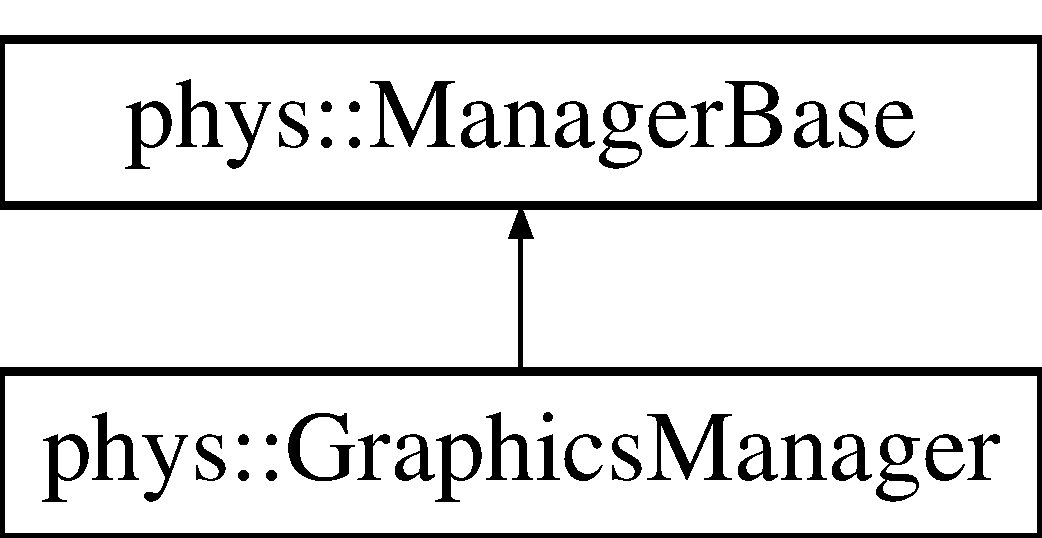
\includegraphics[height=2cm]{dd/d63/classphys_1_1GraphicsManager}
\end{center}
\end{figure}
\subsection*{Public Member Functions}
\begin{DoxyCompactItemize}
\item 
\hyperlink{classphys_1_1GraphicsManager_a744d8dc01a75c3a7653f10271c24cb89}{GraphicsManager} (\hyperlink{classphys_1_1World}{World} $\ast$GameWorld\_\-)
\begin{DoxyCompactList}\small\item\em Basic constructor. \item\end{DoxyCompactList}\item 
\hyperlink{classphys_1_1GraphicsManager_ad08d99ea5279fc4aab9615aba536e9cb}{GraphicsManager} (\hyperlink{classphys_1_1World}{World} $\ast$GameWorld\_\-, const \hyperlink{namespacephys_a460f6bc24c8dd347b05e0366ae34f34a}{Whole} \&Width\_\-, const \hyperlink{namespacephys_a460f6bc24c8dd347b05e0366ae34f34a}{Whole} \&Height\_\-, const bool \&FullScreen\_\-)
\begin{DoxyCompactList}\small\item\em Versatile Constructor. \item\end{DoxyCompactList}\item 
bool \hyperlink{classphys_1_1GraphicsManager_ad126eedb81e3f0304731ddd33b617593}{getFullscreen} () const 
\begin{DoxyCompactList}\small\item\em Gets the Fullscreen Setting. \item\end{DoxyCompactList}\item 
void \hyperlink{classphys_1_1GraphicsManager_aafcf1824190e44d42a9bfbea9cfbe1b2}{setFullscreen} (const bool \&Fullscreen\_\-)
\begin{DoxyCompactList}\small\item\em Set the Fullscreen Setting. \item\end{DoxyCompactList}\item 
\hyperlink{namespacephys_a460f6bc24c8dd347b05e0366ae34f34a}{Whole} \hyperlink{classphys_1_1GraphicsManager_a38ee0f8a8a7d8ba861b1c6cfe579443e}{getRenderHeight} () const 
\begin{DoxyCompactList}\small\item\em Gets the Height of the Rendering Area. \item\end{DoxyCompactList}\item 
void \hyperlink{classphys_1_1GraphicsManager_a8d59e9a8aa2ae7f520d388a4c70f0623}{setRenderHeight} (const \hyperlink{namespacephys_a460f6bc24c8dd347b05e0366ae34f34a}{Whole} \&Height\_\-)
\begin{DoxyCompactList}\small\item\em Sets the Height. \item\end{DoxyCompactList}\item 
\hyperlink{namespacephys_a460f6bc24c8dd347b05e0366ae34f34a}{Whole} \hyperlink{classphys_1_1GraphicsManager_a9e1ce1f9f8bcff7712fd5beaf7cf2337}{getRenderWidth} () const 
\begin{DoxyCompactList}\small\item\em Gets the Width of the Rendering Area. \item\end{DoxyCompactList}\item 
void \hyperlink{classphys_1_1GraphicsManager_aea5fb5808a23fa29c8522c396ac0d6b5}{setRenderWidth} (const \hyperlink{namespacephys_a460f6bc24c8dd347b05e0366ae34f34a}{Whole} \&Width\_\-)
\begin{DoxyCompactList}\small\item\em Sets the Width. \item\end{DoxyCompactList}\item 
void \hyperlink{classphys_1_1GraphicsManager_ac6feb044d9ab394f3e65d51026a899a6}{setRenderResolution} (const \hyperlink{namespacephys_a460f6bc24c8dd347b05e0366ae34f34a}{Whole} \&Width\_\-, const \hyperlink{namespacephys_a460f6bc24c8dd347b05e0366ae34f34a}{Whole} \&Height\_\-)
\begin{DoxyCompactList}\small\item\em Changes the X and Y Resolution at the same time. \item\end{DoxyCompactList}\item 
bool \hyperlink{classphys_1_1GraphicsManager_adcded385b6442aa5da6097f1edd5471a}{ShowGraphicsSettingDialog} ()
\begin{DoxyCompactList}\small\item\em \hyperlink{structThis}{This} Shows an Engine Generated Configuration Screen. \item\end{DoxyCompactList}\item 
virtual void \hyperlink{classphys_1_1GraphicsManager_a554572de5d1cdce37aa1760d6e6e039c}{Initialize} ()
\begin{DoxyCompactList}\small\item\em Empty Initializor. \item\end{DoxyCompactList}\item 
virtual void \hyperlink{classphys_1_1GraphicsManager_a72e5dc563c6947cded348f19d3df41ee}{DoMainLoopItems} ()
\begin{DoxyCompactList}\small\item\em \hyperlink{structThis}{This} is where the rendering takes place. \item\end{DoxyCompactList}\item 
virtual \hyperlink{classphys_1_1ManagerBase_aaa6ccddf23892eaccb898529414f80a5}{ManagerTypeName} \hyperlink{classphys_1_1GraphicsManager_abf48faad2e09cd564442e66bc0473e58}{GetType} () const 
\begin{DoxyCompactList}\small\item\em \hyperlink{structThis}{This} returns the type of this manager. \item\end{DoxyCompactList}\item 
virtual bool \hyperlink{classphys_1_1GraphicsManager_ae2330172be150cd4d12aa2ed62b0474c}{PostMainLoopItems} ()
\begin{DoxyCompactList}\small\item\em \hyperlink{structThis}{This} is derived from and uses the \hyperlink{classphys_1_1ManagerBase}{ManagerBase} to perform the the post main loop callbacks. \item\end{DoxyCompactList}\end{DoxyCompactItemize}


\subsection{Detailed Description}
\hyperlink{structThis}{This} is intended to store basic graphics setting for the user. \hyperlink{structThis}{This} stores x/y resolution, fullscreen and in the future other settings. \hyperlink{structThis}{This} is intended to make it easy for developers to pass/move around complex graphics settings. We hope to eventually include other items like shader settings, rendering API, and maybe other settings too. 

Definition at line 60 of file graphicsmanager.h.



\subsection{Constructor \& Destructor Documentation}
\hypertarget{classphys_1_1GraphicsManager_a744d8dc01a75c3a7653f10271c24cb89}{
\index{phys::GraphicsManager@{phys::GraphicsManager}!GraphicsManager@{GraphicsManager}}
\index{GraphicsManager@{GraphicsManager}!phys::GraphicsManager@{phys::GraphicsManager}}
\subsubsection[{GraphicsManager}]{\setlength{\rightskip}{0pt plus 5cm}phys::GraphicsManager::GraphicsManager ({\bf World} $\ast$ {\em GameWorld\_\-})}}
\label{dd/d63/classphys_1_1GraphicsManager_a744d8dc01a75c3a7653f10271c24cb89}


Basic constructor. 


\begin{DoxyParams}{Parameters}
\item[{\em GameWorld\_\-}]\hyperlink{structThis}{This} is a pointer to the \hyperlink{classphys_1_1World}{phys::World} to which this GrapchisManager will be attached\end{DoxyParams}
\hyperlink{structThis}{This} creates a basic Graphics Settings with resolution 640x480 with fullscreen set to false 

Definition at line 55 of file graphicsmanager.cpp.

\hypertarget{classphys_1_1GraphicsManager_ad08d99ea5279fc4aab9615aba536e9cb}{
\index{phys::GraphicsManager@{phys::GraphicsManager}!GraphicsManager@{GraphicsManager}}
\index{GraphicsManager@{GraphicsManager}!phys::GraphicsManager@{phys::GraphicsManager}}
\subsubsection[{GraphicsManager}]{\setlength{\rightskip}{0pt plus 5cm}phys::GraphicsManager::GraphicsManager ({\bf World} $\ast$ {\em GameWorld\_\-}, \/  const {\bf Whole} \& {\em Width\_\-}, \/  const {\bf Whole} \& {\em Height\_\-}, \/  const bool \& {\em FullScreen\_\-})}}
\label{dd/d63/classphys_1_1GraphicsManager_ad08d99ea5279fc4aab9615aba536e9cb}


Versatile Constructor. 


\begin{DoxyParams}{Parameters}
\item[{\em GameWorld\_\-}]\hyperlink{structThis}{This} is a pointer to the \hyperlink{classphys_1_1World}{phys::World} to which this GrapchisManager will be attached \item[{\em Width\_\-}]The desired width. \item[{\em Height\_\-}]The desired height. \item[{\em FullScreen\_\-}]True if fullscreen, false if not.\end{DoxyParams}
\hyperlink{structThis}{This} creates a Graphics Settings with resolution and fullscreen passed into to it. Be careful that the settings selected are appropriate. Many mobile devices do not support windows, and many screens do not support arbitrary resolutions in fullscreen mode. 

Definition at line 60 of file graphicsmanager.cpp.



\subsection{Member Function Documentation}
\hypertarget{classphys_1_1GraphicsManager_a72e5dc563c6947cded348f19d3df41ee}{
\index{phys::GraphicsManager@{phys::GraphicsManager}!DoMainLoopItems@{DoMainLoopItems}}
\index{DoMainLoopItems@{DoMainLoopItems}!phys::GraphicsManager@{phys::GraphicsManager}}
\subsubsection[{DoMainLoopItems}]{\setlength{\rightskip}{0pt plus 5cm}void phys::GraphicsManager::DoMainLoopItems ()\hspace{0.3cm}{\ttfamily  \mbox{[}virtual\mbox{]}}}}
\label{dd/d63/classphys_1_1GraphicsManager_a72e5dc563c6947cded348f19d3df41ee}


\hyperlink{structThis}{This} is where the rendering takes place. 

\hyperlink{structThis}{This} does the rendering for the game using all the actors in the actormanager. 

Implements \hyperlink{classphys_1_1ManagerBase_aa9e13a3f7c398b708f0f242610b5abf7}{phys::ManagerBase}.



Definition at line 144 of file graphicsmanager.cpp.

\hypertarget{classphys_1_1GraphicsManager_ad126eedb81e3f0304731ddd33b617593}{
\index{phys::GraphicsManager@{phys::GraphicsManager}!getFullscreen@{getFullscreen}}
\index{getFullscreen@{getFullscreen}!phys::GraphicsManager@{phys::GraphicsManager}}
\subsubsection[{getFullscreen}]{\setlength{\rightskip}{0pt plus 5cm}bool phys::GraphicsManager::getFullscreen () const}}
\label{dd/d63/classphys_1_1GraphicsManager_ad126eedb81e3f0304731ddd33b617593}


Gets the Fullscreen Setting. 

Gets the Fullscreen Setting \begin{DoxyReturn}{Returns}
\hyperlink{structThis}{This} returns a bool, true if fullscreen is set, false otherwise 
\end{DoxyReturn}


Definition at line 78 of file graphicsmanager.cpp.

\hypertarget{classphys_1_1GraphicsManager_a38ee0f8a8a7d8ba861b1c6cfe579443e}{
\index{phys::GraphicsManager@{phys::GraphicsManager}!getRenderHeight@{getRenderHeight}}
\index{getRenderHeight@{getRenderHeight}!phys::GraphicsManager@{phys::GraphicsManager}}
\subsubsection[{getRenderHeight}]{\setlength{\rightskip}{0pt plus 5cm}{\bf Whole} phys::GraphicsManager::getRenderHeight () const}}
\label{dd/d63/classphys_1_1GraphicsManager_a38ee0f8a8a7d8ba861b1c6cfe579443e}


Gets the Height of the Rendering Area. 

Gets the Height of the Rendering Area \begin{DoxyReturn}{Returns}
\hyperlink{structThis}{This} returns the Height of the Rendering Area 
\end{DoxyReturn}


Definition at line 94 of file graphicsmanager.cpp.

\hypertarget{classphys_1_1GraphicsManager_a9e1ce1f9f8bcff7712fd5beaf7cf2337}{
\index{phys::GraphicsManager@{phys::GraphicsManager}!getRenderWidth@{getRenderWidth}}
\index{getRenderWidth@{getRenderWidth}!phys::GraphicsManager@{phys::GraphicsManager}}
\subsubsection[{getRenderWidth}]{\setlength{\rightskip}{0pt plus 5cm}{\bf Whole} phys::GraphicsManager::getRenderWidth () const}}
\label{dd/d63/classphys_1_1GraphicsManager_a9e1ce1f9f8bcff7712fd5beaf7cf2337}


Gets the Width of the Rendering Area. 

Gets the Width of the Rendering Area \begin{DoxyReturn}{Returns}
\hyperlink{structThis}{This} returns the Width of the Rendering Area 
\end{DoxyReturn}


Definition at line 99 of file graphicsmanager.cpp.

\hypertarget{classphys_1_1GraphicsManager_abf48faad2e09cd564442e66bc0473e58}{
\index{phys::GraphicsManager@{phys::GraphicsManager}!GetType@{GetType}}
\index{GetType@{GetType}!phys::GraphicsManager@{phys::GraphicsManager}}
\subsubsection[{GetType}]{\setlength{\rightskip}{0pt plus 5cm}{\bf ManagerBase::ManagerTypeName} phys::GraphicsManager::GetType () const\hspace{0.3cm}{\ttfamily  \mbox{[}virtual\mbox{]}}}}
\label{dd/d63/classphys_1_1GraphicsManager_abf48faad2e09cd564442e66bc0473e58}


\hyperlink{structThis}{This} returns the type of this manager. 

\begin{DoxyReturn}{Returns}
\hyperlink{structThis}{This} returns ManagerTypeName::GraphicsManager 
\end{DoxyReturn}


Implements \hyperlink{classphys_1_1ManagerBase_aff400b6599db635e24796d8221e9a0e3}{phys::ManagerBase}.



Definition at line 166 of file graphicsmanager.cpp.

\hypertarget{classphys_1_1GraphicsManager_a554572de5d1cdce37aa1760d6e6e039c}{
\index{phys::GraphicsManager@{phys::GraphicsManager}!Initialize@{Initialize}}
\index{Initialize@{Initialize}!phys::GraphicsManager@{phys::GraphicsManager}}
\subsubsection[{Initialize}]{\setlength{\rightskip}{0pt plus 5cm}void phys::GraphicsManager::Initialize ()\hspace{0.3cm}{\ttfamily  \mbox{[}virtual\mbox{]}}}}
\label{dd/d63/classphys_1_1GraphicsManager_a554572de5d1cdce37aa1760d6e6e039c}


Empty Initializor. 

\hyperlink{structThis}{This} specific initializor is unneeded, but we implement it for compatibility. It also exists in case a derived class wants to override it for some reason 

Implements \hyperlink{classphys_1_1ManagerBase_a57dd8e54e767427d5bdcc86dc66d73ed}{phys::ManagerBase}.



Definition at line 139 of file graphicsmanager.cpp.

\hypertarget{classphys_1_1GraphicsManager_ae2330172be150cd4d12aa2ed62b0474c}{
\index{phys::GraphicsManager@{phys::GraphicsManager}!PostMainLoopItems@{PostMainLoopItems}}
\index{PostMainLoopItems@{PostMainLoopItems}!phys::GraphicsManager@{phys::GraphicsManager}}
\subsubsection[{PostMainLoopItems}]{\setlength{\rightskip}{0pt plus 5cm}bool phys::GraphicsManager::PostMainLoopItems ()\hspace{0.3cm}{\ttfamily  \mbox{[}virtual\mbox{]}}}}
\label{dd/d63/classphys_1_1GraphicsManager_ae2330172be150cd4d12aa2ed62b0474c}


\hyperlink{structThis}{This} is derived from and uses the \hyperlink{classphys_1_1ManagerBase}{ManagerBase} to perform the the post main loop callbacks. 

\begin{DoxyReturn}{Returns}
\hyperlink{structThis}{This} returns a true or false depending on what the callback returns 
\end{DoxyReturn}


Reimplemented from \hyperlink{classphys_1_1ManagerBase_afc3572602f96bdeb8215c386ff870820}{phys::ManagerBase}.



Definition at line 169 of file graphicsmanager.cpp.

\hypertarget{classphys_1_1GraphicsManager_aafcf1824190e44d42a9bfbea9cfbe1b2}{
\index{phys::GraphicsManager@{phys::GraphicsManager}!setFullscreen@{setFullscreen}}
\index{setFullscreen@{setFullscreen}!phys::GraphicsManager@{phys::GraphicsManager}}
\subsubsection[{setFullscreen}]{\setlength{\rightskip}{0pt plus 5cm}void phys::GraphicsManager::setFullscreen (const bool \& {\em Fullscreen\_\-})}}
\label{dd/d63/classphys_1_1GraphicsManager_aafcf1824190e44d42a9bfbea9cfbe1b2}


Set the Fullscreen Setting. 

Set the Fullscreen Setting 
\begin{DoxyParams}{Parameters}
\item[{\em Fullscreen\_\-}]\hyperlink{structThis}{This} accepts a bool. True for fullscreen, false for windowed \end{DoxyParams}


\begin{Desc}
\item[\hyperlink{todo__todo000009}{Todo}]TODO: Need to attempt to switch to fullscreen here \end{Desc}
\begin{Desc}
\item[\hyperlink{todo__todo000010}{Todo}]TODO: We really should double check that going into fullscreen worked the way we wanted, this fails in too many games \end{Desc}




Definition at line 84 of file graphicsmanager.cpp.

\hypertarget{classphys_1_1GraphicsManager_a8d59e9a8aa2ae7f520d388a4c70f0623}{
\index{phys::GraphicsManager@{phys::GraphicsManager}!setRenderHeight@{setRenderHeight}}
\index{setRenderHeight@{setRenderHeight}!phys::GraphicsManager@{phys::GraphicsManager}}
\subsubsection[{setRenderHeight}]{\setlength{\rightskip}{0pt plus 5cm}void phys::GraphicsManager::setRenderHeight (const {\bf Whole} \& {\em Height\_\-})}}
\label{dd/d63/classphys_1_1GraphicsManager_a8d59e9a8aa2ae7f520d388a4c70f0623}


Sets the Height. 

Set the Render Height inside the window in windowed mode, set the resolution of the screen in fullscreen 
\begin{DoxyParams}{Parameters}
\item[{\em Height\_\-}]\hyperlink{structThis}{This} accepts a Whole. \end{DoxyParams}


\begin{Desc}
\item[\hyperlink{todo__todo000011}{Todo}]TODO: Need to attempt to update resolution here \end{Desc}




Definition at line 104 of file graphicsmanager.cpp.

\hypertarget{classphys_1_1GraphicsManager_ac6feb044d9ab394f3e65d51026a899a6}{
\index{phys::GraphicsManager@{phys::GraphicsManager}!setRenderResolution@{setRenderResolution}}
\index{setRenderResolution@{setRenderResolution}!phys::GraphicsManager@{phys::GraphicsManager}}
\subsubsection[{setRenderResolution}]{\setlength{\rightskip}{0pt plus 5cm}void phys::GraphicsManager::setRenderResolution (const {\bf Whole} \& {\em Width\_\-}, \/  const {\bf Whole} \& {\em Height\_\-})}}
\label{dd/d63/classphys_1_1GraphicsManager_ac6feb044d9ab394f3e65d51026a899a6}


Changes the X and Y Resolution at the same time. 

\hyperlink{structThis}{This} should be useful in situations where it is not possible to update the width and hright separately. 
\begin{DoxyParams}{Parameters}
\item[{\em Width\_\-}]The new desired Width for the rendering area as a whole number \item[{\em Height\_\-}]The new desired Width for the rendering area as a whole number \end{DoxyParams}


\begin{Desc}
\item[\hyperlink{todo__todo000013}{Todo}]TODO: Need to attempt to update resolution here \end{Desc}




Definition at line 116 of file graphicsmanager.cpp.

\hypertarget{classphys_1_1GraphicsManager_aea5fb5808a23fa29c8522c396ac0d6b5}{
\index{phys::GraphicsManager@{phys::GraphicsManager}!setRenderWidth@{setRenderWidth}}
\index{setRenderWidth@{setRenderWidth}!phys::GraphicsManager@{phys::GraphicsManager}}
\subsubsection[{setRenderWidth}]{\setlength{\rightskip}{0pt plus 5cm}void phys::GraphicsManager::setRenderWidth (const {\bf Whole} \& {\em Width\_\-})}}
\label{dd/d63/classphys_1_1GraphicsManager_aea5fb5808a23fa29c8522c396ac0d6b5}


Sets the Width. 

Set the Render Width inside the window in windowed mode, set the resolution of the screen in fullscreen 
\begin{DoxyParams}{Parameters}
\item[{\em Width\_\-}]\hyperlink{structThis}{This} accepts a Whole. \end{DoxyParams}


\begin{Desc}
\item[\hyperlink{todo__todo000012}{Todo}]TODO: Need to attempt to update resolution here \end{Desc}




Definition at line 110 of file graphicsmanager.cpp.

\hypertarget{classphys_1_1GraphicsManager_adcded385b6442aa5da6097f1edd5471a}{
\index{phys::GraphicsManager@{phys::GraphicsManager}!ShowGraphicsSettingDialog@{ShowGraphicsSettingDialog}}
\index{ShowGraphicsSettingDialog@{ShowGraphicsSettingDialog}!phys::GraphicsManager@{phys::GraphicsManager}}
\subsubsection[{ShowGraphicsSettingDialog}]{\setlength{\rightskip}{0pt plus 5cm}bool phys::GraphicsManager::ShowGraphicsSettingDialog ()}}
\label{dd/d63/classphys_1_1GraphicsManager_adcded385b6442aa5da6097f1edd5471a}


\hyperlink{structThis}{This} Shows an Engine Generated Configuration Screen. 

\hyperlink{structThis}{This} could look like and could offer just about any option to the user. It is loosely expected to show Graphical Configuration options, like Vsync and Resolution, But it might ask some really silly stuff. I think this would be fine for smaller simpler apps Which have no other way to configure such things, but any sizable project should develop their own way to expose and manage user settings. 

Definition at line 126 of file graphicsmanager.cpp.



The documentation for this class was generated from the following files:\begin{DoxyCompactItemize}
\item 
graphicsmanager.h\item 
graphicsmanager.cpp\end{DoxyCompactItemize}

\hypertarget{classphys_1_1GravityField}{
\section{phys::GravityField Class Reference}
\label{d4/d8a/classphys_1_1GravityField}\index{phys::GravityField@{phys::GravityField}}
}


This is a gravity field implementation of the \hyperlink{classphys_1_1AreaEffect}{AreaEffect} class.  




{\ttfamily \#include $<$areaeffect.h$>$}

Inheritance diagram for phys::GravityField:\begin{figure}[H]
\begin{center}
\leavevmode
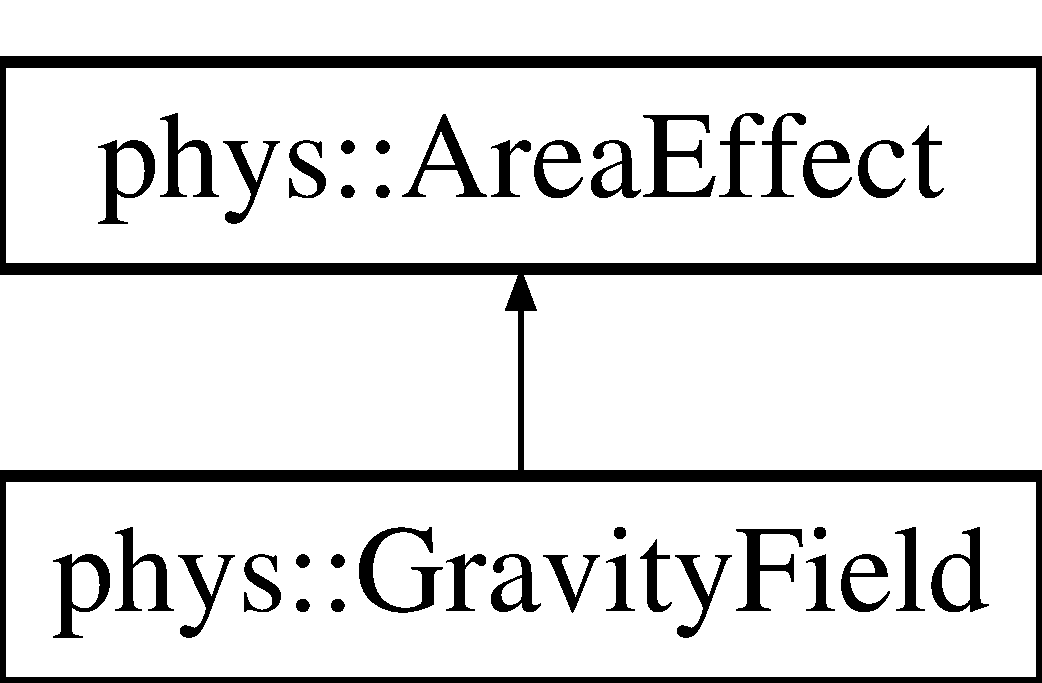
\includegraphics[height=2.000000cm]{d4/d8a/classphys_1_1GravityField}
\end{center}
\end{figure}
\subsection*{Public Member Functions}
\begin{DoxyCompactItemize}
\item 
\hyperlink{classphys_1_1GravityField_a9093176e954b4c631d0757a553971cfd}{GravityField} (const \hyperlink{namespacephys_aa03900411993de7fbfec4789bc1d392e}{String} \&name, \hyperlink{classphys_1_1Vector3}{Vector3} Location)
\begin{DoxyCompactList}\small\item\em Constructor. \item\end{DoxyCompactList}\item 
\hyperlink{classphys_1_1GravityField_ae41a656b247a2982da2e1ae666c605d0}{$\sim$GravityField} ()
\begin{DoxyCompactList}\small\item\em Destructor. \item\end{DoxyCompactList}\item 
virtual void \hyperlink{classphys_1_1GravityField_a0322cb1635bbcb951493d9e17cc9acb1}{ApplyEffect} ()
\begin{DoxyCompactList}\small\item\em Applies the effect this field has to object inside. \item\end{DoxyCompactList}\item 
void \hyperlink{classphys_1_1GravityField_a7cebfe216580e9ef607a2ea070cbeaec}{SetFieldGravity} (\hyperlink{classphys_1_1Vector3}{Vector3} Gravity)
\begin{DoxyCompactList}\small\item\em Sets the gravity force for this field. \item\end{DoxyCompactList}\item 
\hyperlink{classphys_1_1Vector3}{Vector3} \hyperlink{classphys_1_1GravityField_ae776978b7e8fa1d656bdb216aa6f2d20}{GetFieldGravity} ()
\begin{DoxyCompactList}\small\item\em Gets the gravity of this field. \item\end{DoxyCompactList}\end{DoxyCompactItemize}
\subsection*{Protected Attributes}
\begin{DoxyCompactItemize}
\item 
\hypertarget{classphys_1_1GravityField_a14084e696d0848db88b4a91413245849}{
\hyperlink{classphys_1_1Vector3}{Vector3} \hyperlink{classphys_1_1GravityField_a14084e696d0848db88b4a91413245849}{Grav}}
\label{d4/d8a/classphys_1_1GravityField_a14084e696d0848db88b4a91413245849}

\begin{DoxyCompactList}\small\item\em The stored value for this fields gravity. \item\end{DoxyCompactList}\end{DoxyCompactItemize}


\subsection{Detailed Description}
This is a gravity field implementation of the \hyperlink{classphys_1_1AreaEffect}{AreaEffect} class. This class is not a gravity well, where gravity is pulling to one point. Instead this class uniformly pulls gravity in one direction that is different from the world gravity. 

Definition at line 251 of file areaeffect.h.



\subsection{Constructor \& Destructor Documentation}
\hypertarget{classphys_1_1GravityField_a9093176e954b4c631d0757a553971cfd}{
\index{phys::GravityField@{phys::GravityField}!GravityField@{GravityField}}
\index{GravityField@{GravityField}!phys::GravityField@{phys::GravityField}}
\subsubsection[{GravityField}]{\setlength{\rightskip}{0pt plus 5cm}phys::GravityField::GravityField (
\begin{DoxyParamCaption}
\item[{const {\bf String} \&}]{ name, }
\item[{{\bf Vector3}}]{ Location}
\end{DoxyParamCaption}
)}}
\label{d4/d8a/classphys_1_1GravityField_a9093176e954b4c631d0757a553971cfd}


Constructor. 

Basic initialization constructor. 
\begin{DoxyParams}{Parameters}
\item[{\em name}]The name of the field. \item[{\em Location}]The location of the AE field. \end{DoxyParams}


Definition at line 540 of file areaeffect.cpp.

\hypertarget{classphys_1_1GravityField_ae41a656b247a2982da2e1ae666c605d0}{
\index{phys::GravityField@{phys::GravityField}!$\sim$GravityField@{$\sim$GravityField}}
\index{$\sim$GravityField@{$\sim$GravityField}!phys::GravityField@{phys::GravityField}}
\subsubsection[{$\sim$GravityField}]{\setlength{\rightskip}{0pt plus 5cm}phys::GravityField::$\sim$GravityField (
\begin{DoxyParamCaption}
{}
\end{DoxyParamCaption}
)}}
\label{d4/d8a/classphys_1_1GravityField_ae41a656b247a2982da2e1ae666c605d0}


Destructor. 

Class destructor. 

Definition at line 544 of file areaeffect.cpp.



\subsection{Member Function Documentation}
\hypertarget{classphys_1_1GravityField_a0322cb1635bbcb951493d9e17cc9acb1}{
\index{phys::GravityField@{phys::GravityField}!ApplyEffect@{ApplyEffect}}
\index{ApplyEffect@{ApplyEffect}!phys::GravityField@{phys::GravityField}}
\subsubsection[{ApplyEffect}]{\setlength{\rightskip}{0pt plus 5cm}void phys::GravityField::ApplyEffect (
\begin{DoxyParamCaption}
{}
\end{DoxyParamCaption}
)\hspace{0.3cm}{\ttfamily  \mbox{[}virtual\mbox{]}}}}
\label{d4/d8a/classphys_1_1GravityField_a0322cb1635bbcb951493d9e17cc9acb1}


Applies the effect this field has to object inside. 

This function defines the behavior for the class. 

Implements \hyperlink{classphys_1_1AreaEffect_a3b285ecfcf9c9200662d510e48dd222a}{phys::AreaEffect}.



Definition at line 548 of file areaeffect.cpp.

\hypertarget{classphys_1_1GravityField_ae776978b7e8fa1d656bdb216aa6f2d20}{
\index{phys::GravityField@{phys::GravityField}!GetFieldGravity@{GetFieldGravity}}
\index{GetFieldGravity@{GetFieldGravity}!phys::GravityField@{phys::GravityField}}
\subsubsection[{GetFieldGravity}]{\setlength{\rightskip}{0pt plus 5cm}{\bf Vector3} phys::GravityField::GetFieldGravity (
\begin{DoxyParamCaption}
{}
\end{DoxyParamCaption}
)}}
\label{d4/d8a/classphys_1_1GravityField_ae776978b7e8fa1d656bdb216aa6f2d20}


Gets the gravity of this field. 

Gets the strength and direction of gravity this field has. \begin{DoxyReturn}{Returns}
Returns a vector3 representing the force and direction of gravity this field has. 
\end{DoxyReturn}


Definition at line 577 of file areaeffect.cpp.

\hypertarget{classphys_1_1GravityField_a7cebfe216580e9ef607a2ea070cbeaec}{
\index{phys::GravityField@{phys::GravityField}!SetFieldGravity@{SetFieldGravity}}
\index{SetFieldGravity@{SetFieldGravity}!phys::GravityField@{phys::GravityField}}
\subsubsection[{SetFieldGravity}]{\setlength{\rightskip}{0pt plus 5cm}void phys::GravityField::SetFieldGravity (
\begin{DoxyParamCaption}
\item[{{\bf Vector3}}]{ Gravity}
\end{DoxyParamCaption}
)}}
\label{d4/d8a/classphys_1_1GravityField_a7cebfe216580e9ef607a2ea070cbeaec}


Sets the gravity force for this field. 

Sets the strength and direction of gravity this field will have. 
\begin{DoxyParams}{Parameters}
\item[{\em Gravity}]The vector3 representing the force and direction of gravity this field will have. \end{DoxyParams}


Definition at line 572 of file areaeffect.cpp.



The documentation for this class was generated from the following files:\begin{DoxyCompactItemize}
\item 
areaeffect.h\item 
areaeffect.cpp\end{DoxyCompactItemize}

\hypertarget{classphys_1_1Hinge2Constraint}{
\section{phys::Hinge2Constraint Class Reference}
\label{d2/d16/classphys_1_1Hinge2Constraint}\index{phys::Hinge2Constraint@{phys::Hinge2Constraint}}
}
Inheritance diagram for phys::Hinge2Constraint:\begin{figure}[H]
\begin{center}
\leavevmode
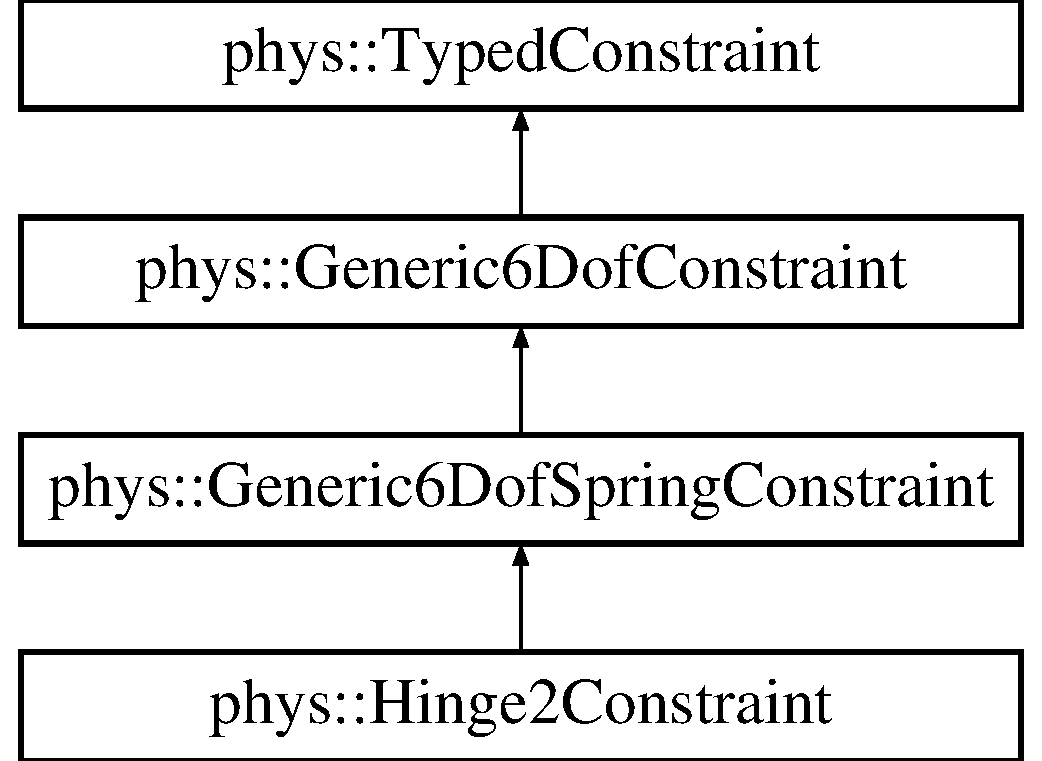
\includegraphics[height=4cm]{d2/d16/classphys_1_1Hinge2Constraint}
\end{center}
\end{figure}
\subsection*{Public Member Functions}
\begin{DoxyCompactItemize}
\item 
\hypertarget{classphys_1_1Hinge2Constraint_a3cc11d107f00c966f7e2c14713ea4e99}{
{\bfseries Hinge2Constraint} (\hyperlink{classphys_1_1ActorRigid}{ActorRigid} $\ast$ActorA, \hyperlink{classphys_1_1ActorRigid}{ActorRigid} $\ast$ActorB, \hyperlink{classphys_1_1Vector3}{Vector3} Anchor, \hyperlink{classphys_1_1Vector3}{Vector3} Axis1, \hyperlink{classphys_1_1Vector3}{Vector3} Axis2)}
\label{d2/d16/classphys_1_1Hinge2Constraint_a3cc11d107f00c966f7e2c14713ea4e99}

\item 
\hypertarget{classphys_1_1Hinge2Constraint_aaf937ddb299b8b47e243e83dfd585e44}{
{\bfseries Hinge2Constraint} (btHinge2Constraint $\ast$Constraint)}
\label{d2/d16/classphys_1_1Hinge2Constraint_aaf937ddb299b8b47e243e83dfd585e44}

\item 
\hypertarget{classphys_1_1Hinge2Constraint_a0510219dca0c79d643411bd1183c5caf}{
void {\bfseries SetUpperLimit} (\hyperlink{namespacephys_af7eb897198d265b8e868f45240230d5f}{Real} Ang1Max)}
\label{d2/d16/classphys_1_1Hinge2Constraint_a0510219dca0c79d643411bd1183c5caf}

\item 
\hypertarget{classphys_1_1Hinge2Constraint_afce03aaa6e238c52027b9ab0e69304b0}{
void {\bfseries SetLowerLimit} (\hyperlink{namespacephys_af7eb897198d265b8e868f45240230d5f}{Real} Ang1Min)}
\label{d2/d16/classphys_1_1Hinge2Constraint_afce03aaa6e238c52027b9ab0e69304b0}

\end{DoxyCompactItemize}
\subsection*{Protected Attributes}
\begin{DoxyCompactItemize}
\item 
\hypertarget{classphys_1_1Hinge2Constraint_aa32c384f4c51895001e4378342d8f45e}{
btHinge2Constraint $\ast$ {\bfseries Hinge2}}
\label{d2/d16/classphys_1_1Hinge2Constraint_aa32c384f4c51895001e4378342d8f45e}

\end{DoxyCompactItemize}


\subsection{Detailed Description}


Definition at line 164 of file constraint.h.



The documentation for this class was generated from the following files:\begin{DoxyCompactItemize}
\item 
constraint.h\item 
constraint.cpp\end{DoxyCompactItemize}

\hypertarget{classphys_1_1HingeConstraint}{
\section{phys::HingeConstraint Class Reference}
\label{d3/d0d/classphys_1_1HingeConstraint}\index{phys::HingeConstraint@{phys::HingeConstraint}}
}
Inheritance diagram for phys::HingeConstraint:\begin{figure}[H]
\begin{center}
\leavevmode
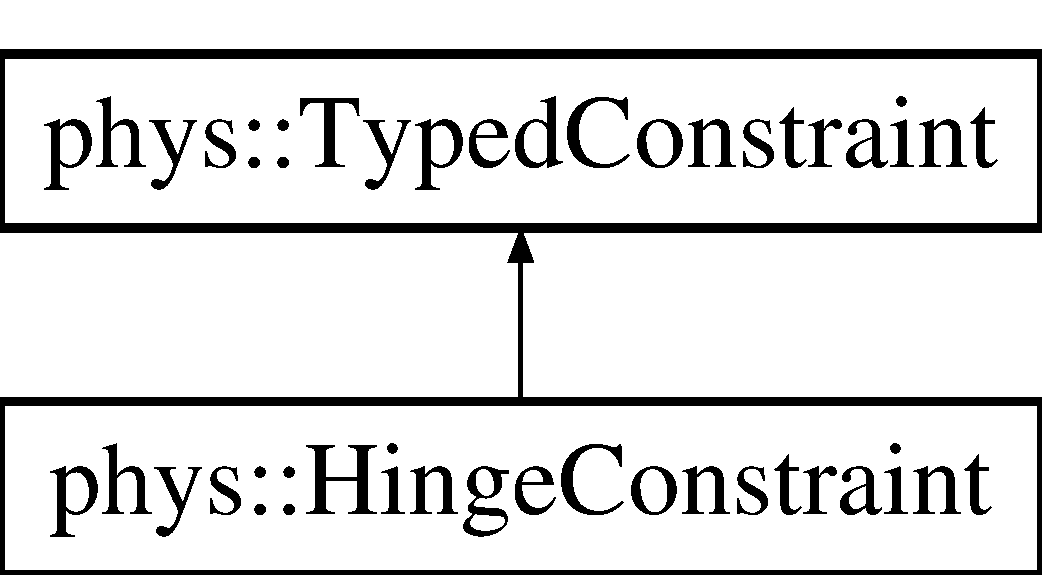
\includegraphics[height=2cm]{d3/d0d/classphys_1_1HingeConstraint}
\end{center}
\end{figure}
\subsection*{Public Member Functions}
\begin{DoxyCompactItemize}
\item 
\hyperlink{classphys_1_1HingeConstraint_a079d149580bb7f60e09532a938352141}{HingeConstraint} (\hyperlink{classphys_1_1ActorRigid}{ActorRigid} $\ast$\hyperlink{classphys_1_1TypedConstraint_a0fefb80c80d433bec9942b851b2f5a8a}{ActorA}, \hyperlink{classphys_1_1ActorRigid}{ActorRigid} $\ast$\hyperlink{classphys_1_1TypedConstraint_a04d2c49698d9a161e92112dd1efc1dcd}{ActorB}, \hyperlink{classphys_1_1Vector3}{Vector3} PivotInA, \hyperlink{classphys_1_1Vector3}{Vector3} PivotInB, \hyperlink{classphys_1_1Vector3}{Vector3} AxisInA, \hyperlink{classphys_1_1Vector3}{Vector3} AxisInB, bool UseReferenceA=false)
\item 
\hyperlink{classphys_1_1HingeConstraint_aa49fe941387343b75d26a3603aafe09e}{HingeConstraint} (\hyperlink{classphys_1_1ActorRigid}{ActorRigid} $\ast$\hyperlink{classphys_1_1TypedConstraint_a0fefb80c80d433bec9942b851b2f5a8a}{ActorA}, \hyperlink{classphys_1_1Vector3}{Vector3} PivotInA, \hyperlink{classphys_1_1Vector3}{Vector3} AxisInA, bool UseReferenceA=false)
\item 
\hyperlink{classphys_1_1HingeConstraint_acf99af18e95c5b42119d91aff8a02a2a}{HingeConstraint} (\hyperlink{classphys_1_1ActorRigid}{ActorRigid} $\ast$\hyperlink{classphys_1_1TypedConstraint_a0fefb80c80d433bec9942b851b2f5a8a}{ActorA}, \hyperlink{classphys_1_1ActorRigid}{ActorRigid} $\ast$\hyperlink{classphys_1_1TypedConstraint_a04d2c49698d9a161e92112dd1efc1dcd}{ActorB}, \hyperlink{classphys_1_1Vector3}{Vector3} VectorA, \hyperlink{classphys_1_1Vector3}{Vector3} VectorB, \hyperlink{classphys_1_1Quaternion}{Quaternion} QuaternionA, \hyperlink{classphys_1_1Quaternion}{Quaternion} QuaternionB, bool UseReferenceA=false)
\item 
\hyperlink{classphys_1_1HingeConstraint_ab326e7128413aa3b737b726b3513c8df}{HingeConstraint} (btHingeConstraint $\ast$Constraint)
\begin{DoxyCompactList}\small\item\em Internal constructor. \item\end{DoxyCompactList}\item 
virtual \hyperlink{classphys_1_1HingeConstraint_af97da06f82fa1903bb20393760f4ae34}{$\sim$HingeConstraint} ()
\begin{DoxyCompactList}\small\item\em Class destructor. \item\end{DoxyCompactList}\item 
\hypertarget{classphys_1_1HingeConstraint_afa922bdd01eaa8e8c1bbafff1c5f7500}{
void {\bfseries SetAPivotLocation} (\hyperlink{classphys_1_1Vector3}{Vector3} Location)}
\label{d3/d0d/classphys_1_1HingeConstraint_afa922bdd01eaa8e8c1bbafff1c5f7500}

\item 
\hypertarget{classphys_1_1HingeConstraint_a6891924d55abb8a68195b4f5b08420b4}{
void {\bfseries SetBPivotLocation} (\hyperlink{classphys_1_1Vector3}{Vector3} Location)}
\label{d3/d0d/classphys_1_1HingeConstraint_a6891924d55abb8a68195b4f5b08420b4}

\item 
\hypertarget{classphys_1_1HingeConstraint_af0c9120692422de58ba6d442a01f22b6}{
void {\bfseries SetAngularOnly} (bool AngularOnly)}
\label{d3/d0d/classphys_1_1HingeConstraint_af0c9120692422de58ba6d442a01f22b6}

\item 
\hypertarget{classphys_1_1HingeConstraint_a43fd81df8530a1bcee46fd52f8b47a28}{
void {\bfseries EnableAngularMotor} (bool EnableMotor, \hyperlink{namespacephys_af7eb897198d265b8e868f45240230d5f}{Real} TargetVelocity, \hyperlink{namespacephys_af7eb897198d265b8e868f45240230d5f}{Real} MaxMotorImpulse)}
\label{d3/d0d/classphys_1_1HingeConstraint_a43fd81df8530a1bcee46fd52f8b47a28}

\item 
\hypertarget{classphys_1_1HingeConstraint_a943ff31d46129143b66744abbb46086f}{
void {\bfseries EnableMotor} (bool EnableMotor)}
\label{d3/d0d/classphys_1_1HingeConstraint_a943ff31d46129143b66744abbb46086f}

\item 
\hypertarget{classphys_1_1HingeConstraint_a944b8ade0a8a1f4853566bc17ebb23ac}{
void {\bfseries SetMaxMotorImpulse} (\hyperlink{namespacephys_af7eb897198d265b8e868f45240230d5f}{Real} MaxMotorImpulse)}
\label{d3/d0d/classphys_1_1HingeConstraint_a944b8ade0a8a1f4853566bc17ebb23ac}

\item 
\hypertarget{classphys_1_1HingeConstraint_a9a9b914a2a64f3cbc09700c61fcdce41}{
void {\bfseries SetMotorTarget} (\hyperlink{classphys_1_1Quaternion}{Quaternion} QuatAInB, \hyperlink{namespacephys_af7eb897198d265b8e868f45240230d5f}{Real} Dt)}
\label{d3/d0d/classphys_1_1HingeConstraint_a9a9b914a2a64f3cbc09700c61fcdce41}

\item 
\hypertarget{classphys_1_1HingeConstraint_a6080b88f14312a509fe089f7c893e62d}{
void {\bfseries SetMotorTarget} (\hyperlink{namespacephys_af7eb897198d265b8e868f45240230d5f}{Real} TargetAngle, \hyperlink{namespacephys_af7eb897198d265b8e868f45240230d5f}{Real} Dt)}
\label{d3/d0d/classphys_1_1HingeConstraint_a6080b88f14312a509fe089f7c893e62d}

\item 
\hypertarget{classphys_1_1HingeConstraint_acabfc495ddd1da39fc1709be32923d1b}{
void {\bfseries SetLimit} (\hyperlink{namespacephys_af7eb897198d265b8e868f45240230d5f}{Real} Low, \hyperlink{namespacephys_af7eb897198d265b8e868f45240230d5f}{Real} High, \hyperlink{namespacephys_af7eb897198d265b8e868f45240230d5f}{Real} Softness=0.9, \hyperlink{namespacephys_af7eb897198d265b8e868f45240230d5f}{Real} BiasFactor=0.3, \hyperlink{namespacephys_af7eb897198d265b8e868f45240230d5f}{Real} RelaxationFactor=1.0)}
\label{d3/d0d/classphys_1_1HingeConstraint_acabfc495ddd1da39fc1709be32923d1b}

\item 
\hypertarget{classphys_1_1HingeConstraint_a25b0004ae13f202cff82f7aaa3722d98}{
void {\bfseries SetAxis} (\hyperlink{classphys_1_1Vector3}{Vector3} AxisInA)}
\label{d3/d0d/classphys_1_1HingeConstraint_a25b0004ae13f202cff82f7aaa3722d98}

\item 
\hypertarget{classphys_1_1HingeConstraint_a06a8ac244cefe64c2ce865e608cb2f41}{
void {\bfseries SetUseFrameOffset} (bool FrameOffset)}
\label{d3/d0d/classphys_1_1HingeConstraint_a06a8ac244cefe64c2ce865e608cb2f41}

\item 
virtual void \hyperlink{classphys_1_1HingeConstraint_adec79d062d67532e3521eaae6b49f877}{SetParam} (int num, \hyperlink{namespacephys_af7eb897198d265b8e868f45240230d5f}{Real} value, int axis=-\/1)
\begin{DoxyCompactList}\small\item\em Provides override of constraint parameters. \item\end{DoxyCompactList}\item 
virtual \hyperlink{namespacephys_af7eb897198d265b8e868f45240230d5f}{Real} \hyperlink{classphys_1_1HingeConstraint_a7e8c001ee6291bf457c9860124cacaf8}{GetParam} (int num, int axis=-\/1)
\begin{DoxyCompactList}\small\item\em Gets value of constraint parameters. \item\end{DoxyCompactList}\end{DoxyCompactItemize}
\subsection*{Protected Attributes}
\begin{DoxyCompactItemize}
\item 
\hypertarget{classphys_1_1HingeConstraint_afa4e4f1595d6420f21449d5e3b730f49}{
btHingeConstraint $\ast$ \hyperlink{classphys_1_1HingeConstraint_afa4e4f1595d6420f21449d5e3b730f49}{Hinge}}
\label{d3/d0d/classphys_1_1HingeConstraint_afa4e4f1595d6420f21449d5e3b730f49}

\begin{DoxyCompactList}\small\item\em Bullet constraint that this class encapsulates. \item\end{DoxyCompactList}\end{DoxyCompactItemize}


\subsection{Detailed Description}


Definition at line 261 of file constraint.h.



\subsection{Constructor \& Destructor Documentation}
\hypertarget{classphys_1_1HingeConstraint_a079d149580bb7f60e09532a938352141}{
\index{phys::HingeConstraint@{phys::HingeConstraint}!HingeConstraint@{HingeConstraint}}
\index{HingeConstraint@{HingeConstraint}!phys::HingeConstraint@{phys::HingeConstraint}}
\subsubsection[{HingeConstraint}]{\setlength{\rightskip}{0pt plus 5cm}phys::HingeConstraint::HingeConstraint ({\bf ActorRigid} $\ast$ {\em ActorA}, \/  {\bf ActorRigid} $\ast$ {\em ActorB}, \/  {\bf Vector3} {\em PivotInA}, \/  {\bf Vector3} {\em PivotInB}, \/  {\bf Vector3} {\em AxisInA}, \/  {\bf Vector3} {\em AxisInB}, \/  bool {\em UseReferenceA} = {\ttfamily false})}}
\label{d3/d0d/classphys_1_1HingeConstraint_a079d149580bb7f60e09532a938352141}

\begin{DoxyParams}{Parameters}
\item[{\em AxisInA}]The orientation for the axis(for ActorA) on which the hinge is to act. For example, a door hinge would be (0.0,1.0,0.0), aka the positive Y axis. \item[{\em AxisInB}]The orientation for the axis(for ActorB) on which the hinge is to act. For example, a door hinge would be (0.0,1.0,0.0), aka the positive Y axis. \item[{\em UseReferenceA}]By default, this constraint uses ActorB's local space as the reference for certain values, such as the rotational limits. This simply controls whether or not it should use ActorA's local space instead. \end{DoxyParams}


Definition at line 333 of file constraint.cpp.

\hypertarget{classphys_1_1HingeConstraint_aa49fe941387343b75d26a3603aafe09e}{
\index{phys::HingeConstraint@{phys::HingeConstraint}!HingeConstraint@{HingeConstraint}}
\index{HingeConstraint@{HingeConstraint}!phys::HingeConstraint@{phys::HingeConstraint}}
\subsubsection[{HingeConstraint}]{\setlength{\rightskip}{0pt plus 5cm}phys::HingeConstraint::HingeConstraint ({\bf ActorRigid} $\ast$ {\em ActorA}, \/  {\bf Vector3} {\em PivotInA}, \/  {\bf Vector3} {\em AxisInA}, \/  bool {\em UseReferenceA} = {\ttfamily false})}}
\label{d3/d0d/classphys_1_1HingeConstraint_aa49fe941387343b75d26a3603aafe09e}

\begin{DoxyParams}{Parameters}
\item[{\em AxisInA}]The axis(for ActorA) on which the hinge is to act. For example, a door hinge would be (0.0,1.0,0.0), aka the positive Y axis. \item[{\em UseReferenceA}]By default, this constraint uses ActorB's local space as the reference for certain values, such as the rotational limits. This simply controls whether or not it should use ActorA's local space instead. \end{DoxyParams}


Definition at line 341 of file constraint.cpp.

\hypertarget{classphys_1_1HingeConstraint_acf99af18e95c5b42119d91aff8a02a2a}{
\index{phys::HingeConstraint@{phys::HingeConstraint}!HingeConstraint@{HingeConstraint}}
\index{HingeConstraint@{HingeConstraint}!phys::HingeConstraint@{phys::HingeConstraint}}
\subsubsection[{HingeConstraint}]{\setlength{\rightskip}{0pt plus 5cm}phys::HingeConstraint::HingeConstraint ({\bf ActorRigid} $\ast$ {\em ActorA}, \/  {\bf ActorRigid} $\ast$ {\em ActorB}, \/  {\bf Vector3} {\em VectorA}, \/  {\bf Vector3} {\em VectorB}, \/  {\bf Quaternion} {\em QuaternionA}, \/  {\bf Quaternion} {\em QuaternionB}, \/  bool {\em UseReferenceA} = {\ttfamily false})}}
\label{d3/d0d/classphys_1_1HingeConstraint_acf99af18e95c5b42119d91aff8a02a2a}

\begin{DoxyParams}{Parameters}
\item[{\em UseReferenceA}]By default, this constraint uses ActorB's local space as the reference for certain values, such as the rotational limits. This simply controls whether or not it should use ActorA's local space instead. \end{DoxyParams}


Definition at line 348 of file constraint.cpp.

\hypertarget{classphys_1_1HingeConstraint_ab326e7128413aa3b737b726b3513c8df}{
\index{phys::HingeConstraint@{phys::HingeConstraint}!HingeConstraint@{HingeConstraint}}
\index{HingeConstraint@{HingeConstraint}!phys::HingeConstraint@{phys::HingeConstraint}}
\subsubsection[{HingeConstraint}]{\setlength{\rightskip}{0pt plus 5cm}phys::HingeConstraint::HingeConstraint (btHingeConstraint $\ast$ {\em Constraint})}}
\label{d3/d0d/classphys_1_1HingeConstraint_ab326e7128413aa3b737b726b3513c8df}


Internal constructor. 

Constructs this class around a pre-\/built bullet constraint. This is an internal only constructor and shouldn't be called manually. 
\begin{DoxyParams}{Parameters}
\item[{\em Constraint}]The constraint to be constructed around. \end{DoxyParams}


Definition at line 356 of file constraint.cpp.

\hypertarget{classphys_1_1HingeConstraint_af97da06f82fa1903bb20393760f4ae34}{
\index{phys::HingeConstraint@{phys::HingeConstraint}!$\sim$HingeConstraint@{$\sim$HingeConstraint}}
\index{$\sim$HingeConstraint@{$\sim$HingeConstraint}!phys::HingeConstraint@{phys::HingeConstraint}}
\subsubsection[{$\sim$HingeConstraint}]{\setlength{\rightskip}{0pt plus 5cm}phys::HingeConstraint::$\sim$HingeConstraint ()\hspace{0.3cm}{\ttfamily  \mbox{[}virtual\mbox{]}}}}
\label{d3/d0d/classphys_1_1HingeConstraint_af97da06f82fa1903bb20393760f4ae34}


Class destructor. 

The class destructor. 

Definition at line 362 of file constraint.cpp.



\subsection{Member Function Documentation}
\hypertarget{classphys_1_1HingeConstraint_a7e8c001ee6291bf457c9860124cacaf8}{
\index{phys::HingeConstraint@{phys::HingeConstraint}!GetParam@{GetParam}}
\index{GetParam@{GetParam}!phys::HingeConstraint@{phys::HingeConstraint}}
\subsubsection[{GetParam}]{\setlength{\rightskip}{0pt plus 5cm}{\bf Real} phys::HingeConstraint::GetParam (int {\em num}, \/  int {\em axis} = {\ttfamily -\/1})\hspace{0.3cm}{\ttfamily  \mbox{[}virtual\mbox{]}}}}
\label{d3/d0d/classphys_1_1HingeConstraint_a7e8c001ee6291bf457c9860124cacaf8}


Gets value of constraint parameters. 

See \hyperlink{classphys_1_1HingeConstraint_adec79d062d67532e3521eaae6b49f877}{SetParam()} for clarification. Gets information on constraint parameters. 
\begin{DoxyParams}{Parameters}
\item[{\em num}]The parameter to get information for. \item[{\em axis}]Optional axis. \end{DoxyParams}
\begin{DoxyReturn}{Returns}
Returns the value for the requested parameter. 
\end{DoxyReturn}


Implements \hyperlink{classphys_1_1TypedConstraint_ab6140d40e9476c3dc46e2802e8097421}{phys::TypedConstraint}.



Definition at line 428 of file constraint.cpp.

\hypertarget{classphys_1_1HingeConstraint_adec79d062d67532e3521eaae6b49f877}{
\index{phys::HingeConstraint@{phys::HingeConstraint}!SetParam@{SetParam}}
\index{SetParam@{SetParam}!phys::HingeConstraint@{phys::HingeConstraint}}
\subsubsection[{SetParam}]{\setlength{\rightskip}{0pt plus 5cm}void phys::HingeConstraint::SetParam (int {\em num}, \/  {\bf Real} {\em value}, \/  int {\em axis} = {\ttfamily -\/1})\hspace{0.3cm}{\ttfamily  \mbox{[}virtual\mbox{]}}}}
\label{d3/d0d/classphys_1_1HingeConstraint_adec79d062d67532e3521eaae6b49f877}


Provides override of constraint parameters. 

Parameters such as ERP and CFM can be altered with this function. Optionally provide axis. 
\begin{DoxyParams}{Parameters}
\item[{\em num}]The parameter to override. \item[{\em value}]The new value for the parameter. \item[{\em axis}]Optional axis. \end{DoxyParams}


Implements \hyperlink{classphys_1_1TypedConstraint_a31a20a74094f0cb8e4f82d1f99725415}{phys::TypedConstraint}.



Definition at line 423 of file constraint.cpp.



The documentation for this class was generated from the following files:\begin{DoxyCompactItemize}
\item 
constraint.h\item 
constraint.cpp\end{DoxyCompactItemize}

\hypertarget{classphys_1_1InputQueryTool}{
\section{phys::InputQueryTool Class Reference}
\label{da/d96/classphys_1_1InputQueryTool}\index{phys::InputQueryTool@{phys::InputQueryTool}}
}


This provides a number of utilities for getting input information.  




{\ttfamily \#include $<$inputquerytool.h$>$}

Inheritance diagram for phys::InputQueryTool:\begin{figure}[H]
\begin{center}
\leavevmode
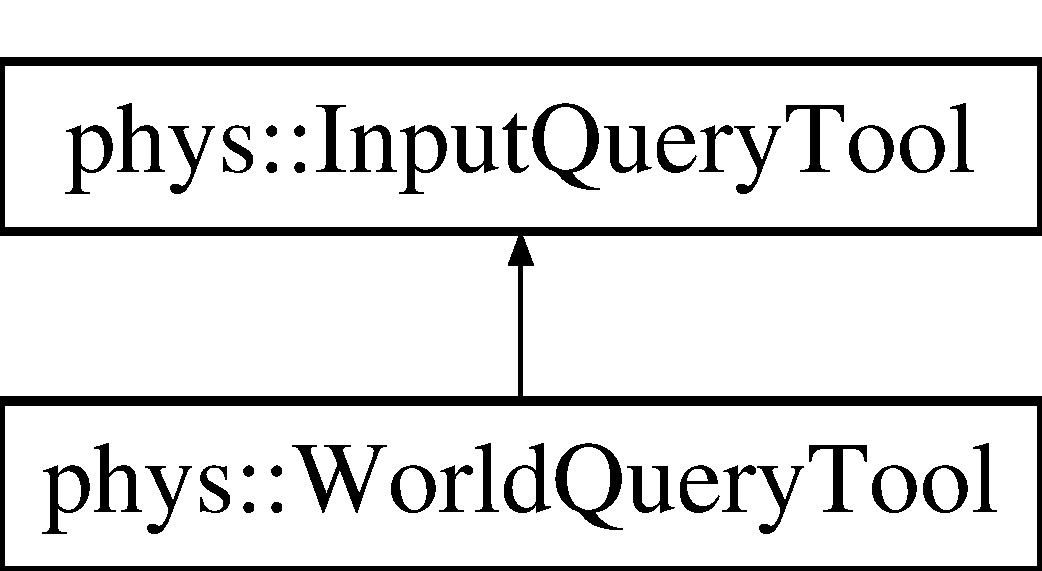
\includegraphics[height=2cm]{da/d96/classphys_1_1InputQueryTool}
\end{center}
\end{figure}
\subsection*{Public Member Functions}
\begin{DoxyCompactItemize}
\item 
\hyperlink{classphys_1_1InputQueryTool_a10a997ec2e072d31808c794542c0516f}{InputQueryTool} ()
\begin{DoxyCompactList}\small\item\em Basic Constructor. \item\end{DoxyCompactList}\item 
\hyperlink{classphys_1_1InputQueryTool_a6a37616800928b691932045ba34759b8}{$\sim$InputQueryTool} ()
\begin{DoxyCompactList}\small\item\em Destructor. \item\end{DoxyCompactList}\item 
\hyperlink{namespacephys_a460f6bc24c8dd347b05e0366ae34f34a}{Whole} \hyperlink{classphys_1_1InputQueryTool_a706c05a974dff509c61440f63bbe9d2d}{GetMouseX} ()
\begin{DoxyCompactList}\small\item\em This gets the X coordinate of the mouse. \item\end{DoxyCompactList}\item 
\hyperlink{namespacephys_a460f6bc24c8dd347b05e0366ae34f34a}{Whole} \hyperlink{classphys_1_1InputQueryTool_acbf87969054ab02e2a7bfc66d9cd4bdd}{GetMouseY} ()
\begin{DoxyCompactList}\small\item\em This gets the Y coordinate of the mouse. \item\end{DoxyCompactList}\item 
\hyperlink{classphys_1_1Vector2}{Vector2} \hyperlink{classphys_1_1InputQueryTool_affd9523f67b542b208e6d36c3395e72b}{GetMouseCoordinates} ()
\begin{DoxyCompactList}\small\item\em This gets a vector2 containing both X and Y coordinates of the mouse. \item\end{DoxyCompactList}\item 
\hyperlink{classphys_1_1Vector2}{Vector2} \hyperlink{classphys_1_1InputQueryTool_aea2da0aeb97353f9d7af75f2a8cb7d91}{GetMousePrevFrameOffset} ()
\begin{DoxyCompactList}\small\item\em This gets the offset location of the mouse since the previous frame. \item\end{DoxyCompactList}\item 
bool \hyperlink{classphys_1_1InputQueryTool_aab9a7be4d95289d828378f7f3d5fc065}{IsMouseButtonPushed} (short unsigned int MouseButton)
\begin{DoxyCompactList}\small\item\em Returns whether a specific Mouse button is pushed. \item\end{DoxyCompactList}\item 
bool \hyperlink{classphys_1_1InputQueryTool_a6f210acb5f4e2fe052b0c3c7c3ec9418}{IsKeyboardButtonPushed} (\hyperlink{classphys_1_1MetaCode_a3e501cbb5bf0f6f1fdb7211465bda8d8}{MetaCode::InputCode} KeyboardButton)
\begin{DoxyCompactList}\small\item\em Returns whether a specific KEyboard button is pushed. \item\end{DoxyCompactList}\item 
\hyperlink{classphys_1_1MetaCode_a2fdfb26b3e50ceb0ccc60bfc4c3d6ac2}{MetaCode::ButtonState} \hyperlink{classphys_1_1InputQueryTool_a1ef8b70af163d8bc703fd16c3fcce22d}{GetMouseButtonState} (short unsigned int MouseButton)
\begin{DoxyCompactList}\small\item\em Gets the button state of the provided mouse button ID. \item\end{DoxyCompactList}\item 
\hyperlink{classphys_1_1MetaCode_a2fdfb26b3e50ceb0ccc60bfc4c3d6ac2}{MetaCode::ButtonState} \hyperlink{classphys_1_1InputQueryTool_ad279cce170ff68ba9f343f6b22b2c621}{GetKeyboardButtonState} (\hyperlink{classphys_1_1MetaCode_a3e501cbb5bf0f6f1fdb7211465bda8d8}{MetaCode::InputCode} KeyboardButton)
\begin{DoxyCompactList}\small\item\em Gets the button state of the provided keyboard button ID. \item\end{DoxyCompactList}\item 
\hyperlink{classphys_1_1MetaCode_af9ba277d1ef071be8861e35c2b7d82d6}{MetaCode::MouseWheelState} \hyperlink{classphys_1_1InputQueryTool_a3b4c3475e48025fbffd18ae3b3acddec}{GetMouseWheelState} ()
\begin{DoxyCompactList}\small\item\em Gets the current status of the mouse wheel. \item\end{DoxyCompactList}\item 
void \hyperlink{classphys_1_1InputQueryTool_a9779d812418f1fddb0880df0c607242b}{GatherEvents} (bool ClearEventsFromEventMgr=false)
\begin{DoxyCompactList}\small\item\em This gathers any user-\/input/event data that might be queryed. \item\end{DoxyCompactList}\end{DoxyCompactItemize}
\subsection*{Protected Attributes}
\begin{DoxyCompactItemize}
\item 
\hyperlink{classphys_1_1World}{World} $\ast$ \hyperlink{classphys_1_1InputQueryTool_ab24a64fc316eefb7e88c1ed75ecee7ea}{GameWorld}
\begin{DoxyCompactList}\small\item\em This is gameworld we will be querying. \item\end{DoxyCompactList}\item 
\hyperlink{namespacephys_a460f6bc24c8dd347b05e0366ae34f34a}{Whole} \hyperlink{classphys_1_1InputQueryTool_a857f0b9ad8bb720f1daf57c9eda6e0fb}{MouseXCache}
\begin{DoxyCompactList}\small\item\em This holds the Mouse X coordinate as of the last time Gather Events was called. \item\end{DoxyCompactList}\item 
\hyperlink{namespacephys_a460f6bc24c8dd347b05e0366ae34f34a}{Whole} \hyperlink{classphys_1_1InputQueryTool_a9378af076545f92b70d853776cc6065c}{MouseYCache}
\begin{DoxyCompactList}\small\item\em This holds the Mouse Y coordinate as of the last time Gather Events was called. \item\end{DoxyCompactList}\item 
\hyperlink{classphys_1_1Vector2}{Vector2} \hyperlink{classphys_1_1InputQueryTool_a379f40bdfb0cbafb84d1dcf297cb1ea3}{MouseCoordinates}
\begin{DoxyCompactList}\small\item\em This stores both mouse coordinates in a \hyperlink{classphys_1_1Vector2}{Vector2}. \item\end{DoxyCompactList}\item 
\hyperlink{classphys_1_1Vector2}{Vector2} \hyperlink{classphys_1_1InputQueryTool_af0e34b7565836f2ebbb15b0d37d10718}{MousePrevFrameOffset}
\begin{DoxyCompactList}\small\item\em This stores the amount the mouse has moved since the previous frame. \item\end{DoxyCompactList}\item 
\hyperlink{classphys_1_1MetaCode_af9ba277d1ef071be8861e35c2b7d82d6}{MetaCode::MouseWheelState} \hyperlink{classphys_1_1InputQueryTool_af6ceb8ea79ea2fe4b881ce715090fa78}{WheelState}
\begin{DoxyCompactList}\small\item\em This stores the current status of the mouse wheel. \item\end{DoxyCompactList}\item 
std::map$<$ unsigned short int, \hyperlink{classphys_1_1MetaCode}{MetaCode} $>$ \hyperlink{classphys_1_1InputQueryTool_a2fddedc3d3ac61a195289b55b0aec972}{MouseButtonCache}
\begin{DoxyCompactList}\small\item\em A place to store which mouse buttons are pushed. \item\end{DoxyCompactList}\item 
std::map$<$ unsigned int, \hyperlink{classphys_1_1MetaCode}{MetaCode} $>$ \hyperlink{classphys_1_1InputQueryTool_afd89b917cb11be11dc990d5ef9ddb2ff}{KeyboardButtonCache}
\begin{DoxyCompactList}\small\item\em A place to store which keys are pressed or not. \item\end{DoxyCompactList}\end{DoxyCompactItemize}
\subsection*{Static Protected Attributes}
\begin{DoxyCompactItemize}
\item 
static const unsigned short int \hyperlink{classphys_1_1InputQueryTool_af5d261bc351f43222db511aacf572409}{MouseButtonLimit} = 16
\begin{DoxyCompactList}\small\item\em This is the mouse button limit of this class. \item\end{DoxyCompactList}\end{DoxyCompactItemize}


\subsection{Detailed Description}
This provides a number of utilities for getting input information. This is useful for quickly and easily getting common input information. 

Definition at line 59 of file inputquerytool.h.



\subsection{Constructor \& Destructor Documentation}
\hypertarget{classphys_1_1InputQueryTool_a10a997ec2e072d31808c794542c0516f}{
\index{phys::InputQueryTool@{phys::InputQueryTool}!InputQueryTool@{InputQueryTool}}
\index{InputQueryTool@{InputQueryTool}!phys::InputQueryTool@{phys::InputQueryTool}}
\subsubsection[{InputQueryTool}]{\setlength{\rightskip}{0pt plus 5cm}phys::InputQueryTool::InputQueryTool ()}}
\label{da/d96/classphys_1_1InputQueryTool_a10a997ec2e072d31808c794542c0516f}


Basic Constructor. 

This creates a \hyperlink{classphys_1_1InputQueryTool}{InputQueryTool} ready to run queries on the input. 

Definition at line 45 of file inputquerytool.cpp.

\hypertarget{classphys_1_1InputQueryTool_a6a37616800928b691932045ba34759b8}{
\index{phys::InputQueryTool@{phys::InputQueryTool}!$\sim$InputQueryTool@{$\sim$InputQueryTool}}
\index{$\sim$InputQueryTool@{$\sim$InputQueryTool}!phys::InputQueryTool@{phys::InputQueryTool}}
\subsubsection[{$\sim$InputQueryTool}]{\setlength{\rightskip}{0pt plus 5cm}phys::InputQueryTool::$\sim$InputQueryTool ()}}
\label{da/d96/classphys_1_1InputQueryTool_a6a37616800928b691932045ba34759b8}


Destructor. 

Deletes everything in the input query tool. 

Definition at line 52 of file inputquerytool.cpp.



\subsection{Member Function Documentation}
\hypertarget{classphys_1_1InputQueryTool_a9779d812418f1fddb0880df0c607242b}{
\index{phys::InputQueryTool@{phys::InputQueryTool}!GatherEvents@{GatherEvents}}
\index{GatherEvents@{GatherEvents}!phys::InputQueryTool@{phys::InputQueryTool}}
\subsubsection[{GatherEvents}]{\setlength{\rightskip}{0pt plus 5cm}void phys::InputQueryTool::GatherEvents (bool {\em ClearEventsFromEventMgr} = {\ttfamily false})}}
\label{da/d96/classphys_1_1InputQueryTool_a9779d812418f1fddb0880df0c607242b}


This gathers any user-\/input/event data that might be queryed. 

This should be called periodcally (ideally in the post user input callback) to allow this to gather data from the \hyperlink{classphys_1_1World}{phys::World} 's event manager. When called this will drop prior event data and any relevant queries will come from this new data. At the caller's discretion this method can properly delete any events pulled from the event manager. \par
 \par
 This runs in linear time relative to the events in the event manager. This will usually be a trivial amount if this is run each iteration and excess events are removed (either by this method or some other form of event cleanup) 
\begin{DoxyParams}{Parameters}
\item[{\em ClearEventsFromEventMgr}]If set to true, This method will properly remove any events it pulls from the event manager. \end{DoxyParams}


\begin{Desc}
\item[\hyperlink{todo__todo000014}{Todo}]Add support for joysticks events to \hyperlink{classphys_1_1InputQueryTool}{InputQueryTool} \end{Desc}




Definition at line 133 of file inputquerytool.cpp.

\hypertarget{classphys_1_1InputQueryTool_ad279cce170ff68ba9f343f6b22b2c621}{
\index{phys::InputQueryTool@{phys::InputQueryTool}!GetKeyboardButtonState@{GetKeyboardButtonState}}
\index{GetKeyboardButtonState@{GetKeyboardButtonState}!phys::InputQueryTool@{phys::InputQueryTool}}
\subsubsection[{GetKeyboardButtonState}]{\setlength{\rightskip}{0pt plus 5cm}{\bf MetaCode::ButtonState} phys::InputQueryTool::GetKeyboardButtonState ({\bf MetaCode::InputCode} {\em KeyboardButton})}}
\label{da/d96/classphys_1_1InputQueryTool_ad279cce170ff68ba9f343f6b22b2c621}


Gets the button state of the provided keyboard button ID. 


\begin{DoxyParams}{Parameters}
\item[{\em KeyboardButton}]The Input code for the keyboard button you wish to query. \end{DoxyParams}
\begin{DoxyReturn}{Returns}
Returns a button state enum representing the button state. 
\end{DoxyReturn}


Definition at line 104 of file inputquerytool.cpp.

\hypertarget{classphys_1_1InputQueryTool_a1ef8b70af163d8bc703fd16c3fcce22d}{
\index{phys::InputQueryTool@{phys::InputQueryTool}!GetMouseButtonState@{GetMouseButtonState}}
\index{GetMouseButtonState@{GetMouseButtonState}!phys::InputQueryTool@{phys::InputQueryTool}}
\subsubsection[{GetMouseButtonState}]{\setlength{\rightskip}{0pt plus 5cm}{\bf MetaCode::ButtonState} phys::InputQueryTool::GetMouseButtonState (short unsigned int {\em MouseButton})}}
\label{da/d96/classphys_1_1InputQueryTool_a1ef8b70af163d8bc703fd16c3fcce22d}


Gets the button state of the provided mouse button ID. 


\begin{DoxyParams}{Parameters}
\item[{\em MouseButton}]The mouse button ID(up to 16) you wish to query.\end{DoxyParams}
Far from all mice have 16 buttons, be sure you know how many buttons the mouse has As this function doesn't perform that check. \begin{DoxyReturn}{Returns}
Returns a button state enum representing the button state. 
\end{DoxyReturn}


Definition at line 80 of file inputquerytool.cpp.

\hypertarget{classphys_1_1InputQueryTool_affd9523f67b542b208e6d36c3395e72b}{
\index{phys::InputQueryTool@{phys::InputQueryTool}!GetMouseCoordinates@{GetMouseCoordinates}}
\index{GetMouseCoordinates@{GetMouseCoordinates}!phys::InputQueryTool@{phys::InputQueryTool}}
\subsubsection[{GetMouseCoordinates}]{\setlength{\rightskip}{0pt plus 5cm}{\bf Vector2} phys::InputQueryTool::GetMouseCoordinates ()}}
\label{da/d96/classphys_1_1InputQueryTool_affd9523f67b542b208e6d36c3395e72b}


This gets a vector2 containing both X and Y coordinates of the mouse. 

If precision is important then you should use the individual coordinate fetching functions instead. \begin{DoxyReturn}{Returns}
This returns a \hyperlink{classphys_1_1Vector2}{Vector2} containing Reals to represent both mouse coordinates. 
\end{DoxyReturn}


Definition at line 62 of file inputquerytool.cpp.

\hypertarget{classphys_1_1InputQueryTool_aea2da0aeb97353f9d7af75f2a8cb7d91}{
\index{phys::InputQueryTool@{phys::InputQueryTool}!GetMousePrevFrameOffset@{GetMousePrevFrameOffset}}
\index{GetMousePrevFrameOffset@{GetMousePrevFrameOffset}!phys::InputQueryTool@{phys::InputQueryTool}}
\subsubsection[{GetMousePrevFrameOffset}]{\setlength{\rightskip}{0pt plus 5cm}{\bf Vector2} phys::InputQueryTool::GetMousePrevFrameOffset ()}}
\label{da/d96/classphys_1_1InputQueryTool_aea2da0aeb97353f9d7af75f2a8cb7d91}


This gets the offset location of the mouse since the previous frame. 

This \hyperlink{classphys_1_1Vector2}{Vector2} is only accurate if this class gathers events every frame. Avoid calling this function otherwise. \begin{DoxyReturn}{Returns}
This returns a vector2 that stores how the mouse has moved since the previous frame. 
\end{DoxyReturn}


Definition at line 65 of file inputquerytool.cpp.

\hypertarget{classphys_1_1InputQueryTool_a3b4c3475e48025fbffd18ae3b3acddec}{
\index{phys::InputQueryTool@{phys::InputQueryTool}!GetMouseWheelState@{GetMouseWheelState}}
\index{GetMouseWheelState@{GetMouseWheelState}!phys::InputQueryTool@{phys::InputQueryTool}}
\subsubsection[{GetMouseWheelState}]{\setlength{\rightskip}{0pt plus 5cm}{\bf MetaCode::MouseWheelState} phys::InputQueryTool::GetMouseWheelState ()}}
\label{da/d96/classphys_1_1InputQueryTool_a3b4c3475e48025fbffd18ae3b3acddec}


Gets the current status of the mouse wheel. 

\begin{DoxyReturn}{Returns}
Returns an enum value representing the current state of the mouse wheel. 
\end{DoxyReturn}


Definition at line 128 of file inputquerytool.cpp.

\hypertarget{classphys_1_1InputQueryTool_a706c05a974dff509c61440f63bbe9d2d}{
\index{phys::InputQueryTool@{phys::InputQueryTool}!GetMouseX@{GetMouseX}}
\index{GetMouseX@{GetMouseX}!phys::InputQueryTool@{phys::InputQueryTool}}
\subsubsection[{GetMouseX}]{\setlength{\rightskip}{0pt plus 5cm}{\bf Whole} phys::InputQueryTool::GetMouseX ()}}
\label{da/d96/classphys_1_1InputQueryTool_a706c05a974dff509c61440f63bbe9d2d}


This gets the X coordinate of the mouse. 

This gets the X location of this mouse. This runs in constant time. \begin{DoxyReturn}{Returns}
This returns a Whole number which represents the X coordinate of the mouse. 
\end{DoxyReturn}


Definition at line 56 of file inputquerytool.cpp.

\hypertarget{classphys_1_1InputQueryTool_acbf87969054ab02e2a7bfc66d9cd4bdd}{
\index{phys::InputQueryTool@{phys::InputQueryTool}!GetMouseY@{GetMouseY}}
\index{GetMouseY@{GetMouseY}!phys::InputQueryTool@{phys::InputQueryTool}}
\subsubsection[{GetMouseY}]{\setlength{\rightskip}{0pt plus 5cm}{\bf Whole} phys::InputQueryTool::GetMouseY ()}}
\label{da/d96/classphys_1_1InputQueryTool_acbf87969054ab02e2a7bfc66d9cd4bdd}


This gets the Y coordinate of the mouse. 

This gets the Y location of this mouse. This runs in constant time. \begin{DoxyReturn}{Returns}
This returns a Whole number which represents the Y coordinate of the mouse. 
\end{DoxyReturn}


Definition at line 59 of file inputquerytool.cpp.

\hypertarget{classphys_1_1InputQueryTool_a6f210acb5f4e2fe052b0c3c7c3ec9418}{
\index{phys::InputQueryTool@{phys::InputQueryTool}!IsKeyboardButtonPushed@{IsKeyboardButtonPushed}}
\index{IsKeyboardButtonPushed@{IsKeyboardButtonPushed}!phys::InputQueryTool@{phys::InputQueryTool}}
\subsubsection[{IsKeyboardButtonPushed}]{\setlength{\rightskip}{0pt plus 5cm}bool phys::InputQueryTool::IsKeyboardButtonPushed ({\bf MetaCode::InputCode} {\em KeyboardButton})}}
\label{da/d96/classphys_1_1InputQueryTool_a6f210acb5f4e2fe052b0c3c7c3ec9418}


Returns whether a specific KEyboard button is pushed. 

This runs in constant time and returns a true is the requested mouse button is pressed. Buttons that are being pressed are considered pressed, and buttons that are being lifted are considered unpressed. 
\begin{DoxyParams}{Parameters}
\item[{\em KeyboardButton}]This is the button that is being checked. \end{DoxyParams}
\begin{DoxyReturn}{Returns}
This returns a bool which is set to true if the requested button is pressed or held down, and false otherwise. 
\end{DoxyReturn}


Definition at line 75 of file inputquerytool.cpp.

\hypertarget{classphys_1_1InputQueryTool_aab9a7be4d95289d828378f7f3d5fc065}{
\index{phys::InputQueryTool@{phys::InputQueryTool}!IsMouseButtonPushed@{IsMouseButtonPushed}}
\index{IsMouseButtonPushed@{IsMouseButtonPushed}!phys::InputQueryTool@{phys::InputQueryTool}}
\subsubsection[{IsMouseButtonPushed}]{\setlength{\rightskip}{0pt plus 5cm}bool phys::InputQueryTool::IsMouseButtonPushed (short unsigned int {\em MouseButton})}}
\label{da/d96/classphys_1_1InputQueryTool_aab9a7be4d95289d828378f7f3d5fc065}


Returns whether a specific Mouse button is pushed. 

This runs in constant time and returns a true is the requested mouse button is pressed. Buttons that are being pressed are considered pressed, and buttons that are being lifted are considered unpressed. This only supports the first 16 mouse buttons at this point (numbered 0 to 15) 
\begin{DoxyParams}{Parameters}
\item[{\em MouseButton}]This is the mouse button that is being checked \end{DoxyParams}

\begin{DoxyExceptions}{Exceptions}
\item[{\em Unsupported mouse button access through InputQueryTool}]This is thrown whenever a mouse button is requested that is beyond the limit that is supported. Currently this limit is 16 \end{DoxyExceptions}
\begin{DoxyReturn}{Returns}
This returns a bool which is set to true if the requested button is pressed or held down, and false otherwise. 
\end{DoxyReturn}


Definition at line 68 of file inputquerytool.cpp.



\subsection{Member Data Documentation}
\hypertarget{classphys_1_1InputQueryTool_ab24a64fc316eefb7e88c1ed75ecee7ea}{
\index{phys::InputQueryTool@{phys::InputQueryTool}!GameWorld@{GameWorld}}
\index{GameWorld@{GameWorld}!phys::InputQueryTool@{phys::InputQueryTool}}
\subsubsection[{GameWorld}]{\setlength{\rightskip}{0pt plus 5cm}{\bf World}$\ast$ {\bf phys::InputQueryTool::GameWorld}\hspace{0.3cm}{\ttfamily  \mbox{[}protected\mbox{]}}}}
\label{da/d96/classphys_1_1InputQueryTool_ab24a64fc316eefb7e88c1ed75ecee7ea}


This is gameworld we will be querying. 

\begin{DoxyInternal}{For internal use only.}
\end{DoxyInternal}


Definition at line 64 of file inputquerytool.h.

\hypertarget{classphys_1_1InputQueryTool_afd89b917cb11be11dc990d5ef9ddb2ff}{
\index{phys::InputQueryTool@{phys::InputQueryTool}!KeyboardButtonCache@{KeyboardButtonCache}}
\index{KeyboardButtonCache@{KeyboardButtonCache}!phys::InputQueryTool@{phys::InputQueryTool}}
\subsubsection[{KeyboardButtonCache}]{\setlength{\rightskip}{0pt plus 5cm}std::map$<$unsigned int,{\bf MetaCode}$>$ {\bf phys::InputQueryTool::KeyboardButtonCache}\hspace{0.3cm}{\ttfamily  \mbox{[}protected\mbox{]}}}}
\label{da/d96/classphys_1_1InputQueryTool_afd89b917cb11be11dc990d5ef9ddb2ff}


A place to store which keys are pressed or not. 

\begin{DoxyInternal}{For internal use only.}
\end{DoxyInternal}


Definition at line 96 of file inputquerytool.h.

\hypertarget{classphys_1_1InputQueryTool_a2fddedc3d3ac61a195289b55b0aec972}{
\index{phys::InputQueryTool@{phys::InputQueryTool}!MouseButtonCache@{MouseButtonCache}}
\index{MouseButtonCache@{MouseButtonCache}!phys::InputQueryTool@{phys::InputQueryTool}}
\subsubsection[{MouseButtonCache}]{\setlength{\rightskip}{0pt plus 5cm}std::map$<$unsigned short int,{\bf MetaCode}$>$ {\bf phys::InputQueryTool::MouseButtonCache}\hspace{0.3cm}{\ttfamily  \mbox{[}protected\mbox{]}}}}
\label{da/d96/classphys_1_1InputQueryTool_a2fddedc3d3ac61a195289b55b0aec972}


A place to store which mouse buttons are pushed. 

\begin{DoxyInternal}{For internal use only.}
\end{DoxyInternal}


Definition at line 92 of file inputquerytool.h.

\hypertarget{classphys_1_1InputQueryTool_af5d261bc351f43222db511aacf572409}{
\index{phys::InputQueryTool@{phys::InputQueryTool}!MouseButtonLimit@{MouseButtonLimit}}
\index{MouseButtonLimit@{MouseButtonLimit}!phys::InputQueryTool@{phys::InputQueryTool}}
\subsubsection[{MouseButtonLimit}]{\setlength{\rightskip}{0pt plus 5cm}const unsigned short int {\bf phys::InputQueryTool::MouseButtonLimit} = 16\hspace{0.3cm}{\ttfamily  \mbox{[}static, protected\mbox{]}}}}
\label{da/d96/classphys_1_1InputQueryTool_af5d261bc351f43222db511aacf572409}


This is the mouse button limit of this class. 

\begin{DoxyInternal}{For internal use only.}
\end{DoxyInternal}


Definition at line 88 of file inputquerytool.h.

\hypertarget{classphys_1_1InputQueryTool_a379f40bdfb0cbafb84d1dcf297cb1ea3}{
\index{phys::InputQueryTool@{phys::InputQueryTool}!MouseCoordinates@{MouseCoordinates}}
\index{MouseCoordinates@{MouseCoordinates}!phys::InputQueryTool@{phys::InputQueryTool}}
\subsubsection[{MouseCoordinates}]{\setlength{\rightskip}{0pt plus 5cm}{\bf Vector2} {\bf phys::InputQueryTool::MouseCoordinates}\hspace{0.3cm}{\ttfamily  \mbox{[}protected\mbox{]}}}}
\label{da/d96/classphys_1_1InputQueryTool_a379f40bdfb0cbafb84d1dcf297cb1ea3}


This stores both mouse coordinates in a \hyperlink{classphys_1_1Vector2}{Vector2}. 

\begin{DoxyInternal}{For internal use only.}
\end{DoxyInternal}


Definition at line 76 of file inputquerytool.h.

\hypertarget{classphys_1_1InputQueryTool_af0e34b7565836f2ebbb15b0d37d10718}{
\index{phys::InputQueryTool@{phys::InputQueryTool}!MousePrevFrameOffset@{MousePrevFrameOffset}}
\index{MousePrevFrameOffset@{MousePrevFrameOffset}!phys::InputQueryTool@{phys::InputQueryTool}}
\subsubsection[{MousePrevFrameOffset}]{\setlength{\rightskip}{0pt plus 5cm}{\bf Vector2} {\bf phys::InputQueryTool::MousePrevFrameOffset}\hspace{0.3cm}{\ttfamily  \mbox{[}protected\mbox{]}}}}
\label{da/d96/classphys_1_1InputQueryTool_af0e34b7565836f2ebbb15b0d37d10718}


This stores the amount the mouse has moved since the previous frame. 

\begin{DoxyInternal}{For internal use only.}
\end{DoxyInternal}


Definition at line 80 of file inputquerytool.h.

\hypertarget{classphys_1_1InputQueryTool_a857f0b9ad8bb720f1daf57c9eda6e0fb}{
\index{phys::InputQueryTool@{phys::InputQueryTool}!MouseXCache@{MouseXCache}}
\index{MouseXCache@{MouseXCache}!phys::InputQueryTool@{phys::InputQueryTool}}
\subsubsection[{MouseXCache}]{\setlength{\rightskip}{0pt plus 5cm}{\bf Whole} {\bf phys::InputQueryTool::MouseXCache}\hspace{0.3cm}{\ttfamily  \mbox{[}protected\mbox{]}}}}
\label{da/d96/classphys_1_1InputQueryTool_a857f0b9ad8bb720f1daf57c9eda6e0fb}


This holds the Mouse X coordinate as of the last time Gather Events was called. 

\begin{DoxyInternal}{For internal use only.}
\end{DoxyInternal}


Definition at line 68 of file inputquerytool.h.

\hypertarget{classphys_1_1InputQueryTool_a9378af076545f92b70d853776cc6065c}{
\index{phys::InputQueryTool@{phys::InputQueryTool}!MouseYCache@{MouseYCache}}
\index{MouseYCache@{MouseYCache}!phys::InputQueryTool@{phys::InputQueryTool}}
\subsubsection[{MouseYCache}]{\setlength{\rightskip}{0pt plus 5cm}{\bf Whole} {\bf phys::InputQueryTool::MouseYCache}\hspace{0.3cm}{\ttfamily  \mbox{[}protected\mbox{]}}}}
\label{da/d96/classphys_1_1InputQueryTool_a9378af076545f92b70d853776cc6065c}


This holds the Mouse Y coordinate as of the last time Gather Events was called. 

\begin{DoxyInternal}{For internal use only.}
\end{DoxyInternal}


Definition at line 72 of file inputquerytool.h.

\hypertarget{classphys_1_1InputQueryTool_af6ceb8ea79ea2fe4b881ce715090fa78}{
\index{phys::InputQueryTool@{phys::InputQueryTool}!WheelState@{WheelState}}
\index{WheelState@{WheelState}!phys::InputQueryTool@{phys::InputQueryTool}}
\subsubsection[{WheelState}]{\setlength{\rightskip}{0pt plus 5cm}{\bf MetaCode::MouseWheelState} {\bf phys::InputQueryTool::WheelState}\hspace{0.3cm}{\ttfamily  \mbox{[}protected\mbox{]}}}}
\label{da/d96/classphys_1_1InputQueryTool_af6ceb8ea79ea2fe4b881ce715090fa78}


This stores the current status of the mouse wheel. 

\begin{DoxyInternal}{For internal use only.}
\end{DoxyInternal}


Definition at line 84 of file inputquerytool.h.



The documentation for this class was generated from the following files:\begin{DoxyCompactItemize}
\item 
inputquerytool.h\item 
inputquerytool.cpp\end{DoxyCompactItemize}

\hypertarget{classphys_1_1debug_1_1InternalDebugDrawer}{
\section{phys::debug::InternalDebugDrawer Class Reference}
\label{db/d27/classphys_1_1debug_1_1InternalDebugDrawer}\index{phys::debug::InternalDebugDrawer@{phys::debug::InternalDebugDrawer}}
}


This is used to draw wireframse for the Physics subsystem.  


\subsection*{Public Member Functions}
\begin{DoxyCompactItemize}
\item 
\hypertarget{classphys_1_1debug_1_1InternalDebugDrawer_a2bdb7e9da99e2d0cd2796cf9c67c3456}{
{\bfseries InternalDebugDrawer} (\hyperlink{classphys_1_1World}{phys::World} $\ast$ParentWorld\_\-, \hyperlink{namespacephys_a460f6bc24c8dd347b05e0366ae34f34a}{Whole} WireFrameCount\_\-=1)}
\label{db/d27/classphys_1_1debug_1_1InternalDebugDrawer_a2bdb7e9da99e2d0cd2796cf9c67c3456}

\item 
\hypertarget{classphys_1_1debug_1_1InternalDebugDrawer_a8a35c3c80fddaaec8e21f737ed1b3938}{
virtual void {\bfseries drawLine} (const btVector3 \&from, const btVector3 \&to, const btVector3 \&color)}
\label{db/d27/classphys_1_1debug_1_1InternalDebugDrawer_a8a35c3c80fddaaec8e21f737ed1b3938}

\item 
\hypertarget{classphys_1_1debug_1_1InternalDebugDrawer_a8b912aaff8dfd9f4e97ffb2d867121b2}{
virtual void {\bfseries drawContactPoint} (const btVector3 \&PointOnB, const btVector3 \&normalOnB, btScalar distance, int lifeTime, const btVector3 \&color)}
\label{db/d27/classphys_1_1debug_1_1InternalDebugDrawer_a8b912aaff8dfd9f4e97ffb2d867121b2}

\item 
\hypertarget{classphys_1_1debug_1_1InternalDebugDrawer_a4e3b4cbc861f76696b4d32f0cf068ea6}{
virtual void {\bfseries reportErrorWarning} (const char $\ast$warningString)}
\label{db/d27/classphys_1_1debug_1_1InternalDebugDrawer_a4e3b4cbc861f76696b4d32f0cf068ea6}

\item 
\hypertarget{classphys_1_1debug_1_1InternalDebugDrawer_a1266d3fad8868ade2d515e9c92e76b4a}{
virtual void {\bfseries draw3dText} (const btVector3 \&location, const char $\ast$textString)}
\label{db/d27/classphys_1_1debug_1_1InternalDebugDrawer_a1266d3fad8868ade2d515e9c92e76b4a}

\item 
\hypertarget{classphys_1_1debug_1_1InternalDebugDrawer_a63059b273ed6031a393b2d994b820bcc}{
virtual void {\bfseries setDebugMode} (int debugMode)}
\label{db/d27/classphys_1_1debug_1_1InternalDebugDrawer_a63059b273ed6031a393b2d994b820bcc}

\item 
\hypertarget{classphys_1_1debug_1_1InternalDebugDrawer_aba329861569d741e970ce5aafb668e84}{
virtual int {\bfseries getDebugMode} () const }
\label{db/d27/classphys_1_1debug_1_1InternalDebugDrawer_aba329861569d741e970ce5aafb668e84}

\item 
\hypertarget{classphys_1_1debug_1_1InternalDebugDrawer_aa1666e636e6ff81813c0b1a85d7bc157}{
virtual \hyperlink{namespacephys_a460f6bc24c8dd347b05e0366ae34f34a}{Whole} {\bfseries GetWireFrameCount} ()}
\label{db/d27/classphys_1_1debug_1_1InternalDebugDrawer_aa1666e636e6ff81813c0b1a85d7bc157}

\item 
\hypertarget{classphys_1_1debug_1_1InternalDebugDrawer_a76922fda7bb3b59d301e50d67e4f3c72}{
virtual void {\bfseries SetWireFrameCount} (\hyperlink{namespacephys_a460f6bc24c8dd347b05e0366ae34f34a}{Whole} WireFrameCount\_\-)}
\label{db/d27/classphys_1_1debug_1_1InternalDebugDrawer_a76922fda7bb3b59d301e50d67e4f3c72}

\end{DoxyCompactItemize}


\subsection{Detailed Description}
This is used to draw wireframse for the Physics subsystem. \begin{DoxyInternal}{For internal use only.}
\end{DoxyInternal}


Definition at line 86 of file world.cpp.



The documentation for this class was generated from the following file:\begin{DoxyCompactItemize}
\item 
world.cpp\end{DoxyCompactItemize}

\hypertarget{classphys_1_1Light}{
\section{phys::Light Class Reference}
\label{dc/df1/classphys_1_1Light}\index{phys::Light@{phys::Light}}
}


This class is the class used for dynamic lighting within the scene.  




{\ttfamily \#include $<$light.h$>$}

Inheritance diagram for phys::Light:\begin{figure}[H]
\begin{center}
\leavevmode
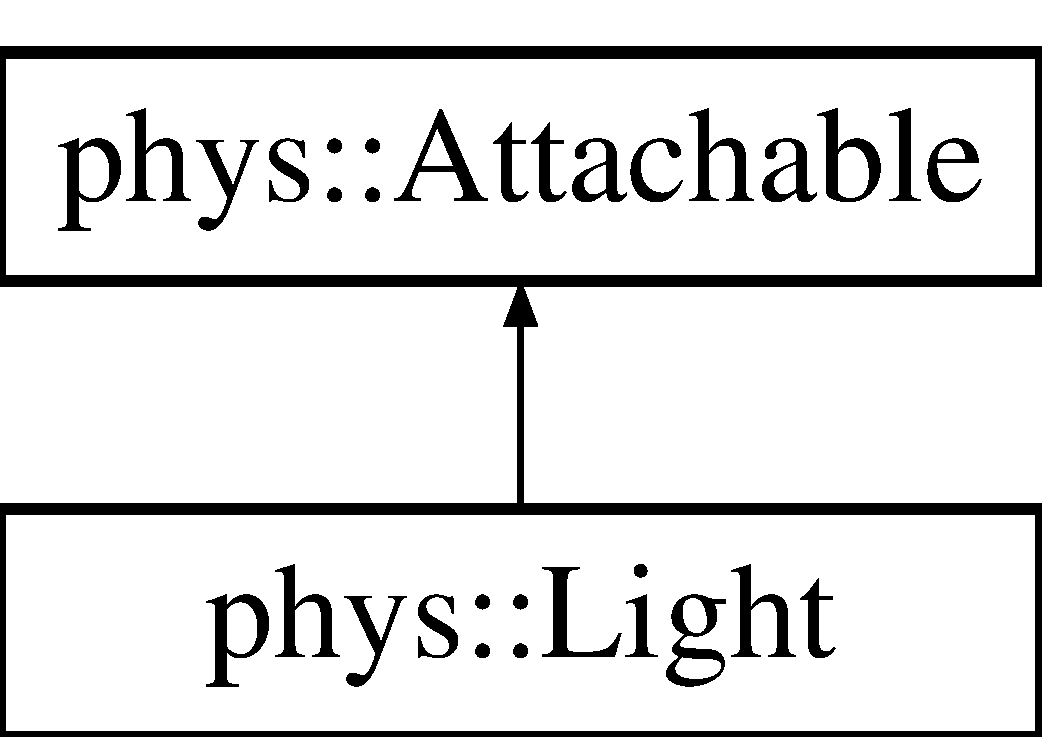
\includegraphics[height=2.000000cm]{dc/df1/classphys_1_1Light}
\end{center}
\end{figure}
\subsection*{Public Types}
\begin{DoxyCompactItemize}
\item 
enum {\bfseries LightType} \{ {\bfseries Directional}, 
{\bfseries Point}, 
{\bfseries Spotlight}
 \}
\end{DoxyCompactItemize}
\subsection*{Public Member Functions}
\begin{DoxyCompactItemize}
\item 
\hyperlink{classphys_1_1Light_a4bcb13aaf1ab92e7df71b565eeec61e4}{Light} (const \hyperlink{namespacephys_aa03900411993de7fbfec4789bc1d392e}{String} \&Name, \hyperlink{classphys_1_1SceneManager}{SceneManager} $\ast$manager)
\begin{DoxyCompactList}\small\item\em Standard initialization constructor. \item\end{DoxyCompactList}\item 
\hyperlink{classphys_1_1Light_a27cfdf1933c6b0054aa4ef8348f56daa}{Light} (Ogre::Light $\ast$light, \hyperlink{classphys_1_1SceneManager}{SceneManager} $\ast$manager)
\begin{DoxyCompactList}\small\item\em Internal Constructor. \item\end{DoxyCompactList}\item 
\hypertarget{classphys_1_1Light_a0ee3882bb8e1e613bd88380a9681af2e}{
virtual \hyperlink{classphys_1_1Light_a0ee3882bb8e1e613bd88380a9681af2e}{$\sim$Light} ()}
\label{dc/df1/classphys_1_1Light_a0ee3882bb8e1e613bd88380a9681af2e}

\begin{DoxyCompactList}\small\item\em Class destructor. \item\end{DoxyCompactList}\item 
\hyperlink{namespacephys_a5ce5049f8b4bf88d6413c47b504ebb31}{ConstString} \& \hyperlink{classphys_1_1Light_a5e85ef1867ad92d589b6cfa96500fcb2}{GetName} () const 
\begin{DoxyCompactList}\small\item\em Gets the name of this light. \item\end{DoxyCompactList}\item 
void \hyperlink{classphys_1_1Light_a87fced0afb0fd44d333c499d41e8568a}{SetType} (Light::LightType Type)
\begin{DoxyCompactList}\small\item\em Sets the type of light this light is. \item\end{DoxyCompactList}\item 
void \hyperlink{classphys_1_1Light_a9c2fcbd1f46ccac815ca7f1b00585c13}{SetPosition} (\hyperlink{classphys_1_1Vector3}{Vector3} Position)
\begin{DoxyCompactList}\small\item\em Sets the location from where the light will originate. \item\end{DoxyCompactList}\item 
void \hyperlink{classphys_1_1Light_a7020d242add6fe47939b3efb3b207f71}{SetDirection} (\hyperlink{classphys_1_1Vector3}{Vector3} Direction)
\begin{DoxyCompactList}\small\item\em Sets the direction the light will originate from. \item\end{DoxyCompactList}\item 
void \hyperlink{classphys_1_1Light_aa54aed6085b348631daa26bc820bb715}{SetDiffuseColour} (\hyperlink{namespacephys_af7eb897198d265b8e868f45240230d5f}{Real} Red, \hyperlink{namespacephys_af7eb897198d265b8e868f45240230d5f}{Real} Green, \hyperlink{namespacephys_af7eb897198d265b8e868f45240230d5f}{Real} Blue)
\begin{DoxyCompactList}\small\item\em Sets the colour for the Diffuse light from this source. \item\end{DoxyCompactList}\item 
void \hyperlink{classphys_1_1Light_ac2e20bac2841e970f231d24d068e7b98}{SetDiffuseColour} (\hyperlink{classphys_1_1ColourValue}{ColourValue} \&Colour)
\begin{DoxyCompactList}\small\item\em Sets the colour for the Diffuse light from this source. \item\end{DoxyCompactList}\item 
void \hyperlink{classphys_1_1Light_a6f2f7b5745e455e7281f7c5e76766c1b}{SetSpecularColour} (\hyperlink{namespacephys_af7eb897198d265b8e868f45240230d5f}{Real} Red, \hyperlink{namespacephys_af7eb897198d265b8e868f45240230d5f}{Real} Green, \hyperlink{namespacephys_af7eb897198d265b8e868f45240230d5f}{Real} Blue)
\begin{DoxyCompactList}\small\item\em Sets the colour for the Specular light from this source. \item\end{DoxyCompactList}\item 
void \hyperlink{classphys_1_1Light_a3e3a407c7f4b26a8d2cd44b9013e8716}{SetSpecularColour} (\hyperlink{classphys_1_1ColourValue}{ColourValue} \&Colour)
\begin{DoxyCompactList}\small\item\em Sets the colour for the Specular light from this source. \item\end{DoxyCompactList}\item 
void \hyperlink{classphys_1_1Light_a22294ff531c0767bc83e7702954e1277}{SetAttenuation} (\hyperlink{namespacephys_af7eb897198d265b8e868f45240230d5f}{Real} Range, \hyperlink{namespacephys_af7eb897198d265b8e868f45240230d5f}{Real} Constant, \hyperlink{namespacephys_af7eb897198d265b8e868f45240230d5f}{Real} Linear, \hyperlink{namespacephys_af7eb897198d265b8e868f45240230d5f}{Real} Quadratic)
\begin{DoxyCompactList}\small\item\em Sets the factors for the attenuation formula applied to this light. \item\end{DoxyCompactList}\item 
void \hyperlink{classphys_1_1Light_a25c79247a42b49d04825bbc76977a134}{SetSpotlightRange} (\hyperlink{namespacephys_af7eb897198d265b8e868f45240230d5f}{Real} InnerAngle, \hyperlink{namespacephys_af7eb897198d265b8e868f45240230d5f}{Real} OuterAngle, \hyperlink{namespacephys_af7eb897198d265b8e868f45240230d5f}{Real} Falloff=1.0)
\begin{DoxyCompactList}\small\item\em Defines the cone of light emitted by a spotlight. \item\end{DoxyCompactList}\item 
void \hyperlink{classphys_1_1Light_a3b812a0181d08f3c30c9a75f13fd6282}{SetSpotlightInnerAngle} (\hyperlink{namespacephys_af7eb897198d265b8e868f45240230d5f}{Real} InnerAngle)
\begin{DoxyCompactList}\small\item\em Sets the Inner angle of the cone of light emitted by a spotlight. \item\end{DoxyCompactList}\item 
void \hyperlink{classphys_1_1Light_a6cab679dfc15d35e3d3b8b229e602fff}{SetSpotlightOuterAngle} (\hyperlink{namespacephys_af7eb897198d265b8e868f45240230d5f}{Real} OuterAngle)
\begin{DoxyCompactList}\small\item\em Sets the Outer angle of the cone of light emitted by a spotlight. \item\end{DoxyCompactList}\item 
void \hyperlink{classphys_1_1Light_a170e0fc23e3a50587a483fa8981b5486}{SetSpotlightFalloff} (\hyperlink{namespacephys_af7eb897198d265b8e868f45240230d5f}{Real} Falloff)
\begin{DoxyCompactList}\small\item\em Sets the rate of falloff of the cone of light emitted by a spotlight. \item\end{DoxyCompactList}\item 
void \hyperlink{classphys_1_1Light_af4a6428b87c443a33261575783a4fb05}{SetPowerScale} (\hyperlink{namespacephys_af7eb897198d265b8e868f45240230d5f}{Real} Power)
\begin{DoxyCompactList}\small\item\em Sets the lights power scale. \item\end{DoxyCompactList}\item 
Light::LightType \hyperlink{classphys_1_1Light_ac404a6c7df9758f8420a8931118f516b}{GetType} () const 
\begin{DoxyCompactList}\small\item\em Gets the type of light that this light is. \item\end{DoxyCompactList}\item 
\hyperlink{classphys_1_1Vector3}{Vector3} \hyperlink{classphys_1_1Light_a9cdf0ce6b98bcb601237aa75d54b9c7d}{GetPosition} () const 
\begin{DoxyCompactList}\small\item\em Gets the current location of the light. \item\end{DoxyCompactList}\item 
\hyperlink{classphys_1_1Vector3}{Vector3} \hyperlink{classphys_1_1Light_afde81fca535417fdb33d23d38117ccac}{GetDirection} () const 
\begin{DoxyCompactList}\small\item\em Gets the currently set direction of the light. \item\end{DoxyCompactList}\item 
\hyperlink{classphys_1_1ColourValue}{ColourValue} \hyperlink{classphys_1_1Light_a75d4d4c33bf0f552e48f280a80dc5fb4}{GetDiffuseColour} () const 
\begin{DoxyCompactList}\small\item\em Gets the current colour of the diffuse light. \item\end{DoxyCompactList}\item 
\hyperlink{classphys_1_1ColourValue}{ColourValue} \hyperlink{classphys_1_1Light_a05c7ab32ddb1acf71a041098fbb9ff35}{GetSpecularColour} () const 
\begin{DoxyCompactList}\small\item\em Gets the current colour of the specular light. \item\end{DoxyCompactList}\item 
\hyperlink{namespacephys_af7eb897198d265b8e868f45240230d5f}{Real} \hyperlink{classphys_1_1Light_ad113608997af66646ed91c28acb9057c}{GetAttenuationRange} () const 
\begin{DoxyCompactList}\small\item\em Gets the absolute range of attenuation in world units. \item\end{DoxyCompactList}\item 
\hyperlink{namespacephys_af7eb897198d265b8e868f45240230d5f}{Real} \hyperlink{classphys_1_1Light_aad30f7fb932b030de7eb15046dea83a7}{GetAttenuationConstant} () const 
\begin{DoxyCompactList}\small\item\em Gets the constant factor of the attenuation. \item\end{DoxyCompactList}\item 
\hyperlink{namespacephys_af7eb897198d265b8e868f45240230d5f}{Real} \hyperlink{classphys_1_1Light_a92245ddc5383fd7f0989866852e36ed8}{GetAttenuationLinear} () const 
\begin{DoxyCompactList}\small\item\em Gets the linear factor of the attentuation. \item\end{DoxyCompactList}\item 
\hyperlink{namespacephys_af7eb897198d265b8e868f45240230d5f}{Real} \hyperlink{classphys_1_1Light_a4ea9693e7ba3f4b6199f132b29e645fa}{GetAttenuationQuadric} () const 
\begin{DoxyCompactList}\small\item\em Gets the quadric factor of the attenuation. \item\end{DoxyCompactList}\item 
\hyperlink{namespacephys_af7eb897198d265b8e868f45240230d5f}{Real} \hyperlink{classphys_1_1Light_a429728b3eb1287806c70a24666705213}{GetSpotlightInnerAngle} () const 
\begin{DoxyCompactList}\small\item\em Gets the Inner angle of the cone of light emitted by this spotlight. \item\end{DoxyCompactList}\item 
\hyperlink{namespacephys_af7eb897198d265b8e868f45240230d5f}{Real} \hyperlink{classphys_1_1Light_a669ab7936e718263d02343ef03333bad}{GetSpotlightOuterAngle} () const 
\begin{DoxyCompactList}\small\item\em Gets the Outer angle of the cone of light emitted by this spotlight. \item\end{DoxyCompactList}\item 
\hyperlink{namespacephys_af7eb897198d265b8e868f45240230d5f}{Real} \hyperlink{classphys_1_1Light_a7682e55d5210c2433060dd9e4f4669ba}{GetSpotlightFalloff} () const 
\begin{DoxyCompactList}\small\item\em Gets the rate of falloff of the cone of light emitted by this spotlight. \item\end{DoxyCompactList}\item 
\hyperlink{namespacephys_af7eb897198d265b8e868f45240230d5f}{Real} \hyperlink{classphys_1_1Light_add09593ac1e57a946aa5f0c319dd56ae}{GetPowerScale} () const 
\begin{DoxyCompactList}\small\item\em Gets the lights power scale. \item\end{DoxyCompactList}\end{DoxyCompactItemize}
\subsection*{Protected Attributes}
\begin{DoxyCompactItemize}
\item 
\hypertarget{classphys_1_1Light_a20fc9136847907955cfb8c1a47d6ec6a}{
Ogre::Light $\ast$ \hyperlink{classphys_1_1Light_a20fc9136847907955cfb8c1a47d6ec6a}{OgreLight}}
\label{dc/df1/classphys_1_1Light_a20fc9136847907955cfb8c1a47d6ec6a}

\begin{DoxyCompactList}\small\item\em The ogre light this class gets it's functionality from. \item\end{DoxyCompactList}\item 
\hypertarget{classphys_1_1Light_a2633fc1795d2a3e2ddddc71674a7eb84}{
\hyperlink{classphys_1_1SceneManager}{SceneManager} $\ast$ \hyperlink{classphys_1_1Light_a2633fc1795d2a3e2ddddc71674a7eb84}{Manager}}
\label{dc/df1/classphys_1_1Light_a2633fc1795d2a3e2ddddc71674a7eb84}

\begin{DoxyCompactList}\small\item\em Pointer to the manager that created this class. \item\end{DoxyCompactList}\end{DoxyCompactItemize}
\subsection*{Friends}
\begin{DoxyCompactItemize}
\item 
\hypertarget{classphys_1_1Light_a1cacd07efb11226da49a7c80569b18e8}{
class {\bfseries WorldNode}}
\label{dc/df1/classphys_1_1Light_a1cacd07efb11226da49a7c80569b18e8}

\end{DoxyCompactItemize}


\subsection{Detailed Description}
This class is the class used for dynamic lighting within the scene. Dynamic lights come in 3 flavors: \par
 Directional -\/ Used to simulate light from a very distant source. Doesn't need a location, only a direction. \hyperlink{classphys_1_1Light}{Light} will hit all objects accordingly from that direction. \par
 Point -\/ Used to simulate local light sources that emit light in all directions. Doesn't need a direction, just a position. \par
 Spotlight -\/ Used to simulate local light sources that emit light in one direction, such as a flashlight. Needs both a position and direction. In addition needs values for falloff. \par
 Note: If attaching a light to a node, all transform information(position and orientation) becomes relative to the nodes transform. 

Definition at line 71 of file light.h.



\subsection{Constructor \& Destructor Documentation}
\hypertarget{classphys_1_1Light_a4bcb13aaf1ab92e7df71b565eeec61e4}{
\index{phys::Light@{phys::Light}!Light@{Light}}
\index{Light@{Light}!phys::Light@{phys::Light}}
\subsubsection[{Light}]{\setlength{\rightskip}{0pt plus 5cm}phys::Light::Light (
\begin{DoxyParamCaption}
\item[{const {\bf String} \&}]{ Name, }
\item[{{\bf SceneManager} $\ast$}]{ manager}
\end{DoxyParamCaption}
)}}
\label{dc/df1/classphys_1_1Light_a4bcb13aaf1ab92e7df71b565eeec61e4}


Standard initialization constructor. 


\begin{DoxyParams}{Parameters}
\item[{\em Name}]The name of this light. \item[{\em manager}]Pointer to the manager that this light is to be used in. \end{DoxyParams}


Definition at line 45 of file light.cpp.

\hypertarget{classphys_1_1Light_a27cfdf1933c6b0054aa4ef8348f56daa}{
\index{phys::Light@{phys::Light}!Light@{Light}}
\index{Light@{Light}!phys::Light@{phys::Light}}
\subsubsection[{Light}]{\setlength{\rightskip}{0pt plus 5cm}phys::Light::Light (
\begin{DoxyParamCaption}
\item[{Ogre::Light $\ast$}]{ light, }
\item[{{\bf SceneManager} $\ast$}]{ manager}
\end{DoxyParamCaption}
)}}
\label{dc/df1/classphys_1_1Light_a27cfdf1933c6b0054aa4ef8348f56daa}


Internal Constructor. 

This constructor should not be called on manually. 
\begin{DoxyParams}{Parameters}
\item[{\em light}]The Ogre light this class is based on. \item[{\em manager}]Pointer to the manager that this light is to be used in. \end{DoxyParams}


Definition at line 52 of file light.cpp.



\subsection{Member Function Documentation}
\hypertarget{classphys_1_1Light_aad30f7fb932b030de7eb15046dea83a7}{
\index{phys::Light@{phys::Light}!GetAttenuationConstant@{GetAttenuationConstant}}
\index{GetAttenuationConstant@{GetAttenuationConstant}!phys::Light@{phys::Light}}
\subsubsection[{GetAttenuationConstant}]{\setlength{\rightskip}{0pt plus 5cm}{\bf Real} phys::Light::GetAttenuationConstant (
\begin{DoxyParamCaption}
{}
\end{DoxyParamCaption}
) const}}
\label{dc/df1/classphys_1_1Light_aad30f7fb932b030de7eb15046dea83a7}


Gets the constant factor of the attenuation. 

\begin{DoxyReturn}{Returns}
Returns a real representing the constant factor of attenuation. 
\end{DoxyReturn}


Definition at line 203 of file light.cpp.

\hypertarget{classphys_1_1Light_a92245ddc5383fd7f0989866852e36ed8}{
\index{phys::Light@{phys::Light}!GetAttenuationLinear@{GetAttenuationLinear}}
\index{GetAttenuationLinear@{GetAttenuationLinear}!phys::Light@{phys::Light}}
\subsubsection[{GetAttenuationLinear}]{\setlength{\rightskip}{0pt plus 5cm}{\bf Real} phys::Light::GetAttenuationLinear (
\begin{DoxyParamCaption}
{}
\end{DoxyParamCaption}
) const}}
\label{dc/df1/classphys_1_1Light_a92245ddc5383fd7f0989866852e36ed8}


Gets the linear factor of the attentuation. 

\begin{DoxyReturn}{Returns}
Returns a real representing the linear factor of attenuation. 
\end{DoxyReturn}


Definition at line 208 of file light.cpp.

\hypertarget{classphys_1_1Light_a4ea9693e7ba3f4b6199f132b29e645fa}{
\index{phys::Light@{phys::Light}!GetAttenuationQuadric@{GetAttenuationQuadric}}
\index{GetAttenuationQuadric@{GetAttenuationQuadric}!phys::Light@{phys::Light}}
\subsubsection[{GetAttenuationQuadric}]{\setlength{\rightskip}{0pt plus 5cm}{\bf Real} phys::Light::GetAttenuationQuadric (
\begin{DoxyParamCaption}
{}
\end{DoxyParamCaption}
) const}}
\label{dc/df1/classphys_1_1Light_a4ea9693e7ba3f4b6199f132b29e645fa}


Gets the quadric factor of the attenuation. 

\begin{DoxyReturn}{Returns}
Returns a real representing the quadric factor of attenuation. 
\end{DoxyReturn}


Definition at line 213 of file light.cpp.

\hypertarget{classphys_1_1Light_ad113608997af66646ed91c28acb9057c}{
\index{phys::Light@{phys::Light}!GetAttenuationRange@{GetAttenuationRange}}
\index{GetAttenuationRange@{GetAttenuationRange}!phys::Light@{phys::Light}}
\subsubsection[{GetAttenuationRange}]{\setlength{\rightskip}{0pt plus 5cm}{\bf Real} phys::Light::GetAttenuationRange (
\begin{DoxyParamCaption}
{}
\end{DoxyParamCaption}
) const}}
\label{dc/df1/classphys_1_1Light_ad113608997af66646ed91c28acb9057c}


Gets the absolute range of attenuation in world units. 

\begin{DoxyReturn}{Returns}
Returns a real representing the absolute range of attenuation. 
\end{DoxyReturn}


Definition at line 198 of file light.cpp.

\hypertarget{classphys_1_1Light_a75d4d4c33bf0f552e48f280a80dc5fb4}{
\index{phys::Light@{phys::Light}!GetDiffuseColour@{GetDiffuseColour}}
\index{GetDiffuseColour@{GetDiffuseColour}!phys::Light@{phys::Light}}
\subsubsection[{GetDiffuseColour}]{\setlength{\rightskip}{0pt plus 5cm}{\bf ColourValue} phys::Light::GetDiffuseColour (
\begin{DoxyParamCaption}
{}
\end{DoxyParamCaption}
) const}}
\label{dc/df1/classphys_1_1Light_a75d4d4c33bf0f552e48f280a80dc5fb4}


Gets the current colour of the diffuse light. 

\begin{DoxyReturn}{Returns}
Returns a colourvalue representing the currently set Diffuse light. 
\end{DoxyReturn}


Definition at line 186 of file light.cpp.

\hypertarget{classphys_1_1Light_afde81fca535417fdb33d23d38117ccac}{
\index{phys::Light@{phys::Light}!GetDirection@{GetDirection}}
\index{GetDirection@{GetDirection}!phys::Light@{phys::Light}}
\subsubsection[{GetDirection}]{\setlength{\rightskip}{0pt plus 5cm}{\bf Vector3} phys::Light::GetDirection (
\begin{DoxyParamCaption}
{}
\end{DoxyParamCaption}
) const}}
\label{dc/df1/classphys_1_1Light_afde81fca535417fdb33d23d38117ccac}


Gets the currently set direction of the light. 

\begin{DoxyReturn}{Returns}
Returns a vector3 representing the set direction of the light. 
\end{DoxyReturn}


Definition at line 180 of file light.cpp.

\hypertarget{classphys_1_1Light_a5e85ef1867ad92d589b6cfa96500fcb2}{
\index{phys::Light@{phys::Light}!GetName@{GetName}}
\index{GetName@{GetName}!phys::Light@{phys::Light}}
\subsubsection[{GetName}]{\setlength{\rightskip}{0pt plus 5cm}{\bf ConstString} \& phys::Light::GetName (
\begin{DoxyParamCaption}
{}
\end{DoxyParamCaption}
) const\hspace{0.3cm}{\ttfamily  \mbox{[}virtual\mbox{]}}}}
\label{dc/df1/classphys_1_1Light_a5e85ef1867ad92d589b6cfa96500fcb2}


Gets the name of this light. 

\begin{DoxyReturn}{Returns}
Returns a string containing the name given to this light. 
\end{DoxyReturn}


Implements \hyperlink{classphys_1_1Attachable_a0a07d727fa2630dc3550fd991ca28256}{phys::Attachable}.



Definition at line 64 of file light.cpp.

\hypertarget{classphys_1_1Light_a9cdf0ce6b98bcb601237aa75d54b9c7d}{
\index{phys::Light@{phys::Light}!GetPosition@{GetPosition}}
\index{GetPosition@{GetPosition}!phys::Light@{phys::Light}}
\subsubsection[{GetPosition}]{\setlength{\rightskip}{0pt plus 5cm}{\bf Vector3} phys::Light::GetPosition (
\begin{DoxyParamCaption}
{}
\end{DoxyParamCaption}
) const}}
\label{dc/df1/classphys_1_1Light_a9cdf0ce6b98bcb601237aa75d54b9c7d}


Gets the current location of the light. 

\begin{DoxyReturn}{Returns}
Returns a vector3 representing the location of the light. 
\end{DoxyReturn}


Definition at line 174 of file light.cpp.

\hypertarget{classphys_1_1Light_add09593ac1e57a946aa5f0c319dd56ae}{
\index{phys::Light@{phys::Light}!GetPowerScale@{GetPowerScale}}
\index{GetPowerScale@{GetPowerScale}!phys::Light@{phys::Light}}
\subsubsection[{GetPowerScale}]{\setlength{\rightskip}{0pt plus 5cm}{\bf Real} phys::Light::GetPowerScale (
\begin{DoxyParamCaption}
{}
\end{DoxyParamCaption}
) const}}
\label{dc/df1/classphys_1_1Light_add09593ac1e57a946aa5f0c319dd56ae}


Gets the lights power scale. 

\begin{DoxyReturn}{Returns}
Returns a real representing the power scale of the light. 
\end{DoxyReturn}


Definition at line 233 of file light.cpp.

\hypertarget{classphys_1_1Light_a05c7ab32ddb1acf71a041098fbb9ff35}{
\index{phys::Light@{phys::Light}!GetSpecularColour@{GetSpecularColour}}
\index{GetSpecularColour@{GetSpecularColour}!phys::Light@{phys::Light}}
\subsubsection[{GetSpecularColour}]{\setlength{\rightskip}{0pt plus 5cm}{\bf ColourValue} phys::Light::GetSpecularColour (
\begin{DoxyParamCaption}
{}
\end{DoxyParamCaption}
) const}}
\label{dc/df1/classphys_1_1Light_a05c7ab32ddb1acf71a041098fbb9ff35}


Gets the current colour of the specular light. 

\begin{DoxyReturn}{Returns}
Returns a colourvalue representing the currently set Specular light. 
\end{DoxyReturn}


Definition at line 192 of file light.cpp.

\hypertarget{classphys_1_1Light_a7682e55d5210c2433060dd9e4f4669ba}{
\index{phys::Light@{phys::Light}!GetSpotlightFalloff@{GetSpotlightFalloff}}
\index{GetSpotlightFalloff@{GetSpotlightFalloff}!phys::Light@{phys::Light}}
\subsubsection[{GetSpotlightFalloff}]{\setlength{\rightskip}{0pt plus 5cm}{\bf Real} phys::Light::GetSpotlightFalloff (
\begin{DoxyParamCaption}
{}
\end{DoxyParamCaption}
) const}}
\label{dc/df1/classphys_1_1Light_a7682e55d5210c2433060dd9e4f4669ba}


Gets the rate of falloff of the cone of light emitted by this spotlight. 

\begin{DoxyReturn}{Returns}
Returns a real representing the falloff of the cone of light. 
\end{DoxyReturn}


Definition at line 228 of file light.cpp.

\hypertarget{classphys_1_1Light_a429728b3eb1287806c70a24666705213}{
\index{phys::Light@{phys::Light}!GetSpotlightInnerAngle@{GetSpotlightInnerAngle}}
\index{GetSpotlightInnerAngle@{GetSpotlightInnerAngle}!phys::Light@{phys::Light}}
\subsubsection[{GetSpotlightInnerAngle}]{\setlength{\rightskip}{0pt plus 5cm}{\bf Real} phys::Light::GetSpotlightInnerAngle (
\begin{DoxyParamCaption}
{}
\end{DoxyParamCaption}
) const}}
\label{dc/df1/classphys_1_1Light_a429728b3eb1287806c70a24666705213}


Gets the Inner angle of the cone of light emitted by this spotlight. 

\begin{DoxyReturn}{Returns}
Returns a real representing the inner angle of this spotlight, in radians. 
\end{DoxyReturn}


Definition at line 218 of file light.cpp.

\hypertarget{classphys_1_1Light_a669ab7936e718263d02343ef03333bad}{
\index{phys::Light@{phys::Light}!GetSpotlightOuterAngle@{GetSpotlightOuterAngle}}
\index{GetSpotlightOuterAngle@{GetSpotlightOuterAngle}!phys::Light@{phys::Light}}
\subsubsection[{GetSpotlightOuterAngle}]{\setlength{\rightskip}{0pt plus 5cm}{\bf Real} phys::Light::GetSpotlightOuterAngle (
\begin{DoxyParamCaption}
{}
\end{DoxyParamCaption}
) const}}
\label{dc/df1/classphys_1_1Light_a669ab7936e718263d02343ef03333bad}


Gets the Outer angle of the cone of light emitted by this spotlight. 

\begin{DoxyReturn}{Returns}
Returns a real representing the outer angle of this spotlight, in radians. 
\end{DoxyReturn}


Definition at line 223 of file light.cpp.

\hypertarget{classphys_1_1Light_ac404a6c7df9758f8420a8931118f516b}{
\index{phys::Light@{phys::Light}!GetType@{GetType}}
\index{GetType@{GetType}!phys::Light@{phys::Light}}
\subsubsection[{GetType}]{\setlength{\rightskip}{0pt plus 5cm}Light::LightType phys::Light::GetType (
\begin{DoxyParamCaption}
{}
\end{DoxyParamCaption}
) const}}
\label{dc/df1/classphys_1_1Light_ac404a6c7df9758f8420a8931118f516b}


Gets the type of light that this light is. 

\begin{DoxyReturn}{Returns}
Returns an enum value for this lights type. 
\end{DoxyReturn}


Definition at line 153 of file light.cpp.

\hypertarget{classphys_1_1Light_a22294ff531c0767bc83e7702954e1277}{
\index{phys::Light@{phys::Light}!SetAttenuation@{SetAttenuation}}
\index{SetAttenuation@{SetAttenuation}!phys::Light@{phys::Light}}
\subsubsection[{SetAttenuation}]{\setlength{\rightskip}{0pt plus 5cm}void phys::Light::SetAttenuation (
\begin{DoxyParamCaption}
\item[{{\bf Real}}]{ Range, }
\item[{{\bf Real}}]{ Constant, }
\item[{{\bf Real}}]{ Linear, }
\item[{{\bf Real}}]{ Quadratic}
\end{DoxyParamCaption}
)}}
\label{dc/df1/classphys_1_1Light_a22294ff531c0767bc83e7702954e1277}


Sets the factors for the attenuation formula applied to this light. 

This function is only necessary when using a spotlight or point type of light. 
\begin{DoxyParams}{Parameters}
\item[{\em Range}]The absolute range of the light in world units. Objects beyond this range will not be influenced by this light. \item[{\em Constant}]The constant of the attenuation, ranging from 0.0 to 1.0. 1.0 means never attenuate, 0.0 is complete attenuation. \item[{\em Linear}]The linear factor of the attentuation, ranging from 0.0 to 1.0. 1.0 means attenuate evenly over the distance. \item[{\em Quadratic}]The Quadratic factor of the attenuation. This value adds curvature to the attenuation. \end{DoxyParams}


Definition at line 119 of file light.cpp.

\hypertarget{classphys_1_1Light_aa54aed6085b348631daa26bc820bb715}{
\index{phys::Light@{phys::Light}!SetDiffuseColour@{SetDiffuseColour}}
\index{SetDiffuseColour@{SetDiffuseColour}!phys::Light@{phys::Light}}
\subsubsection[{SetDiffuseColour}]{\setlength{\rightskip}{0pt plus 5cm}void phys::Light::SetDiffuseColour (
\begin{DoxyParamCaption}
\item[{{\bf Real}}]{ Red, }
\item[{{\bf Real}}]{ Green, }
\item[{{\bf Real}}]{ Blue}
\end{DoxyParamCaption}
)}}
\label{dc/df1/classphys_1_1Light_aa54aed6085b348631daa26bc820bb715}


Sets the colour for the Diffuse light from this source. 

When rendering the final color of an object values of the colours of 3 types of lights are taken into account. The 3 types are: Diffuse, Specular, and Ambient. 
\begin{DoxyParams}{Parameters}
\item[{\em Red}]Real in the range of 0.0 to 1.0 determining the amount of red in the colour. \item[{\em Red}]green in the range of 0.0 to 1.0 determining the amount of green in the colour. \item[{\em Red}]blue in the range of 0.0 to 1.0 determining the amount of blue in the colour. \end{DoxyParams}


Definition at line 99 of file light.cpp.

\hypertarget{classphys_1_1Light_ac2e20bac2841e970f231d24d068e7b98}{
\index{phys::Light@{phys::Light}!SetDiffuseColour@{SetDiffuseColour}}
\index{SetDiffuseColour@{SetDiffuseColour}!phys::Light@{phys::Light}}
\subsubsection[{SetDiffuseColour}]{\setlength{\rightskip}{0pt plus 5cm}void phys::Light::SetDiffuseColour (
\begin{DoxyParamCaption}
\item[{{\bf ColourValue} \&}]{ Colour}
\end{DoxyParamCaption}
)}}
\label{dc/df1/classphys_1_1Light_ac2e20bac2841e970f231d24d068e7b98}


Sets the colour for the Diffuse light from this source. 

This allows the setting of Diffuse color by a premade \hyperlink{classphys_1_1ColourValue}{ColourValue}. 
\begin{DoxyParams}{Parameters}
\item[{\em Colour}]\hyperlink{classphys_1_1ColourValue}{ColourValue} representing the color of the light to be set. \end{DoxyParams}


Definition at line 104 of file light.cpp.

\hypertarget{classphys_1_1Light_a7020d242add6fe47939b3efb3b207f71}{
\index{phys::Light@{phys::Light}!SetDirection@{SetDirection}}
\index{SetDirection@{SetDirection}!phys::Light@{phys::Light}}
\subsubsection[{SetDirection}]{\setlength{\rightskip}{0pt plus 5cm}void phys::Light::SetDirection (
\begin{DoxyParamCaption}
\item[{{\bf Vector3}}]{ Direction}
\end{DoxyParamCaption}
)}}
\label{dc/df1/classphys_1_1Light_a7020d242add6fe47939b3efb3b207f71}


Sets the direction the light will originate from. 


\begin{DoxyParams}{Parameters}
\item[{\em Direction}]A vector3 representing the direction the light will come from. \end{DoxyParams}


Definition at line 94 of file light.cpp.

\hypertarget{classphys_1_1Light_a9c2fcbd1f46ccac815ca7f1b00585c13}{
\index{phys::Light@{phys::Light}!SetPosition@{SetPosition}}
\index{SetPosition@{SetPosition}!phys::Light@{phys::Light}}
\subsubsection[{SetPosition}]{\setlength{\rightskip}{0pt plus 5cm}void phys::Light::SetPosition (
\begin{DoxyParamCaption}
\item[{{\bf Vector3}}]{ Position}
\end{DoxyParamCaption}
)}}
\label{dc/df1/classphys_1_1Light_a9c2fcbd1f46ccac815ca7f1b00585c13}


Sets the location from where the light will originate. 


\begin{DoxyParams}{Parameters}
\item[{\em Position}]A vector3 representing the location to set the light. \end{DoxyParams}


Definition at line 89 of file light.cpp.

\hypertarget{classphys_1_1Light_af4a6428b87c443a33261575783a4fb05}{
\index{phys::Light@{phys::Light}!SetPowerScale@{SetPowerScale}}
\index{SetPowerScale@{SetPowerScale}!phys::Light@{phys::Light}}
\subsubsection[{SetPowerScale}]{\setlength{\rightskip}{0pt plus 5cm}void phys::Light::SetPowerScale (
\begin{DoxyParamCaption}
\item[{{\bf Real}}]{ Power}
\end{DoxyParamCaption}
)}}
\label{dc/df1/classphys_1_1Light_af4a6428b87c443a33261575783a4fb05}


Sets the lights power scale. 

The power scale of the light is a scaling factor indicating the relative power of the light. 
\begin{DoxyParams}{Parameters}
\item[{\em Power}]Real representing the factor by which to scale the power of the light. \end{DoxyParams}


Definition at line 148 of file light.cpp.

\hypertarget{classphys_1_1Light_a6f2f7b5745e455e7281f7c5e76766c1b}{
\index{phys::Light@{phys::Light}!SetSpecularColour@{SetSpecularColour}}
\index{SetSpecularColour@{SetSpecularColour}!phys::Light@{phys::Light}}
\subsubsection[{SetSpecularColour}]{\setlength{\rightskip}{0pt plus 5cm}void phys::Light::SetSpecularColour (
\begin{DoxyParamCaption}
\item[{{\bf Real}}]{ Red, }
\item[{{\bf Real}}]{ Green, }
\item[{{\bf Real}}]{ Blue}
\end{DoxyParamCaption}
)}}
\label{dc/df1/classphys_1_1Light_a6f2f7b5745e455e7281f7c5e76766c1b}


Sets the colour for the Specular light from this source. 

When rendering the final color of an object values of the colours of 3 types of lights are taken into account. The 3 types are: Diffuse, Specular, and Ambient. 
\begin{DoxyParams}{Parameters}
\item[{\em Red}]Real in the range of 0.0 to 1.0 determining the amount of red in the colour. \item[{\em Red}]green in the range of 0.0 to 1.0 determining the amount of green in the colour. \item[{\em Red}]blue in the range of 0.0 to 1.0 determining the amount of blue in the colour. \end{DoxyParams}


Definition at line 109 of file light.cpp.

\hypertarget{classphys_1_1Light_a3e3a407c7f4b26a8d2cd44b9013e8716}{
\index{phys::Light@{phys::Light}!SetSpecularColour@{SetSpecularColour}}
\index{SetSpecularColour@{SetSpecularColour}!phys::Light@{phys::Light}}
\subsubsection[{SetSpecularColour}]{\setlength{\rightskip}{0pt plus 5cm}void phys::Light::SetSpecularColour (
\begin{DoxyParamCaption}
\item[{{\bf ColourValue} \&}]{ Colour}
\end{DoxyParamCaption}
)}}
\label{dc/df1/classphys_1_1Light_a3e3a407c7f4b26a8d2cd44b9013e8716}


Sets the colour for the Specular light from this source. 

This allows the setting of Specular color by a premade \hyperlink{classphys_1_1ColourValue}{ColourValue}. 
\begin{DoxyParams}{Parameters}
\item[{\em Colour}]\hyperlink{classphys_1_1ColourValue}{ColourValue} representing the color of the light to be set. \end{DoxyParams}


Definition at line 114 of file light.cpp.

\hypertarget{classphys_1_1Light_a170e0fc23e3a50587a483fa8981b5486}{
\index{phys::Light@{phys::Light}!SetSpotlightFalloff@{SetSpotlightFalloff}}
\index{SetSpotlightFalloff@{SetSpotlightFalloff}!phys::Light@{phys::Light}}
\subsubsection[{SetSpotlightFalloff}]{\setlength{\rightskip}{0pt plus 5cm}void phys::Light::SetSpotlightFalloff (
\begin{DoxyParamCaption}
\item[{{\bf Real}}]{ Falloff}
\end{DoxyParamCaption}
)}}
\label{dc/df1/classphys_1_1Light_a170e0fc23e3a50587a483fa8981b5486}


Sets the rate of falloff of the cone of light emitted by a spotlight. 


\begin{DoxyParams}{Parameters}
\item[{\em Falloff}]The rate of falloff between the inner and outer cones. 1.0 means linear falloff. Less means slower falloff and higher means faster falloff. \end{DoxyParams}


Definition at line 143 of file light.cpp.

\hypertarget{classphys_1_1Light_a3b812a0181d08f3c30c9a75f13fd6282}{
\index{phys::Light@{phys::Light}!SetSpotlightInnerAngle@{SetSpotlightInnerAngle}}
\index{SetSpotlightInnerAngle@{SetSpotlightInnerAngle}!phys::Light@{phys::Light}}
\subsubsection[{SetSpotlightInnerAngle}]{\setlength{\rightskip}{0pt plus 5cm}void phys::Light::SetSpotlightInnerAngle (
\begin{DoxyParamCaption}
\item[{{\bf Real}}]{ InnerAngle}
\end{DoxyParamCaption}
)}}
\label{dc/df1/classphys_1_1Light_a3b812a0181d08f3c30c9a75f13fd6282}


Sets the Inner angle of the cone of light emitted by a spotlight. 


\begin{DoxyParams}{Parameters}
\item[{\em InnerAngle}]Angle of the inner cone. \end{DoxyParams}


Definition at line 131 of file light.cpp.

\hypertarget{classphys_1_1Light_a6cab679dfc15d35e3d3b8b229e602fff}{
\index{phys::Light@{phys::Light}!SetSpotlightOuterAngle@{SetSpotlightOuterAngle}}
\index{SetSpotlightOuterAngle@{SetSpotlightOuterAngle}!phys::Light@{phys::Light}}
\subsubsection[{SetSpotlightOuterAngle}]{\setlength{\rightskip}{0pt plus 5cm}void phys::Light::SetSpotlightOuterAngle (
\begin{DoxyParamCaption}
\item[{{\bf Real}}]{ OuterAngle}
\end{DoxyParamCaption}
)}}
\label{dc/df1/classphys_1_1Light_a6cab679dfc15d35e3d3b8b229e602fff}


Sets the Outer angle of the cone of light emitted by a spotlight. 


\begin{DoxyParams}{Parameters}
\item[{\em OuterAngle}]Angle of the outer cone. \end{DoxyParams}


Definition at line 137 of file light.cpp.

\hypertarget{classphys_1_1Light_a25c79247a42b49d04825bbc76977a134}{
\index{phys::Light@{phys::Light}!SetSpotlightRange@{SetSpotlightRange}}
\index{SetSpotlightRange@{SetSpotlightRange}!phys::Light@{phys::Light}}
\subsubsection[{SetSpotlightRange}]{\setlength{\rightskip}{0pt plus 5cm}void phys::Light::SetSpotlightRange (
\begin{DoxyParamCaption}
\item[{{\bf Real}}]{ InnerAngle, }
\item[{{\bf Real}}]{ OuterAngle, }
\item[{{\bf Real}}]{ Falloff = {\ttfamily 1.0}}
\end{DoxyParamCaption}
)}}
\label{dc/df1/classphys_1_1Light_a25c79247a42b49d04825bbc76977a134}


Defines the cone of light emitted by a spotlight. 

InnerAngle and OuterAngle should be input as Radians. 
\begin{DoxyParams}{Parameters}
\item[{\em InnerAngle}]Angle of the inner cone. \item[{\em OuterAngle}]Angle of the outer cone. \item[{\em Falloff}]The rate of falloff between the inner and outer cones. 1.0 means linear falloff. Less means slower falloff and higher means faster falloff. \end{DoxyParams}


Definition at line 124 of file light.cpp.

\hypertarget{classphys_1_1Light_a87fced0afb0fd44d333c499d41e8568a}{
\index{phys::Light@{phys::Light}!SetType@{SetType}}
\index{SetType@{SetType}!phys::Light@{phys::Light}}
\subsubsection[{SetType}]{\setlength{\rightskip}{0pt plus 5cm}void phys::Light::SetType (
\begin{DoxyParamCaption}
\item[{Light::LightType}]{ Type}
\end{DoxyParamCaption}
)}}
\label{dc/df1/classphys_1_1Light_a87fced0afb0fd44d333c499d41e8568a}


Sets the type of light this light is. 

The light types are listed with the class info. Types are Directional, Point, and Spotlight. 
\begin{DoxyParams}{Parameters}
\item[{\em Type}]The enum value representing the type of light this is. \end{DoxyParams}


Definition at line 69 of file light.cpp.



The documentation for this class was generated from the following files:\begin{DoxyCompactItemize}
\item 
light.h\item 
light.cpp\end{DoxyCompactItemize}

\hypertarget{classphys_1_1internal_1_1Line3D}{
\section{phys::internal::Line3D Class Reference}
\label{d4/db5/classphys_1_1internal_1_1Line3D}\index{phys::internal::Line3D@{phys::internal::Line3D}}
}


Does the bulk of the work that that the \hyperlink{classphys_1_1LineGroup}{phys::LineGroup} performs.  


\subsection*{Public Member Functions}
\begin{DoxyCompactItemize}
\item 
\hyperlink{classphys_1_1internal_1_1Line3D_ab22b8f5fae0bb2585b1031adfff424bd}{Line3D} (void)
\begin{DoxyCompactList}\small\item\em Default Constructor. \item\end{DoxyCompactList}\item 
\hyperlink{classphys_1_1internal_1_1Line3D_acddc95dd5f319d6afc68260af8bea39c}{$\sim$Line3D} (void)
\begin{DoxyCompactList}\small\item\em Destructor. \item\end{DoxyCompactList}\item 
void \hyperlink{classphys_1_1internal_1_1Line3D_aeb3b828b35b4c8ed76158285be6ddc67}{addPoint} (const Vector3 \&p)
\begin{DoxyCompactList}\small\item\em This adds a point to the list of what should be rendered. \item\end{DoxyCompactList}\item 
const Vector3 \& \hyperlink{classphys_1_1internal_1_1Line3D_a190af0e38be28297ed2f6a7aecf0c316}{getPoint} (\hyperlink{namespacephys_a460f6bc24c8dd347b05e0366ae34f34a}{Whole} index) const 
\begin{DoxyCompactList}\small\item\em Access a specific point by index. \item\end{DoxyCompactList}\item 
\hyperlink{namespacephys_a460f6bc24c8dd347b05e0366ae34f34a}{Whole} \hyperlink{classphys_1_1internal_1_1Line3D_ab72a9dab3a355035c24c15e4a737ea2f}{getNumPoints} (void) const 
\begin{DoxyCompactList}\small\item\em How many points are in this \hyperlink{classphys_1_1internal_1_1Line3D}{Line3D}. \item\end{DoxyCompactList}\item 
void \hyperlink{classphys_1_1internal_1_1Line3D_a4b2dec1619e4456ab0cb034ad34eb9d1}{updatePoint} (\hyperlink{namespacephys_a460f6bc24c8dd347b05e0366ae34f34a}{Whole} index, const Vector3 \&value)
\begin{DoxyCompactList}\small\item\em Change an existing point. \item\end{DoxyCompactList}\item 
void \hyperlink{classphys_1_1internal_1_1Line3D_a0320e600b9f363036c63eb47527bb854}{drawLine} (Vector3 \&start, Vector3 \&end)
\begin{DoxyCompactList}\small\item\em Adds two points. \item\end{DoxyCompactList}\item 
void \hyperlink{classphys_1_1internal_1_1Line3D_a008f0874c2213002e0c39330561f80f2}{drawLines} (void)
\begin{DoxyCompactList}\small\item\em Renders this. \item\end{DoxyCompactList}\item 
\hyperlink{namespacephys_af7eb897198d265b8e868f45240230d5f}{Real} \hyperlink{classphys_1_1internal_1_1Line3D_a04b77721c599bb368c791da7621fc814}{getSquaredViewDepth} (const Camera $\ast$cam) const 
\begin{DoxyCompactList}\small\item\em Not Used. \item\end{DoxyCompactList}\item 
\hyperlink{namespacephys_af7eb897198d265b8e868f45240230d5f}{Real} \hyperlink{classphys_1_1internal_1_1Line3D_a3fdd0ff2b7b22cebc71f796431afc7c8}{getBoundingRadius} (void) const 
\begin{DoxyCompactList}\small\item\em How big would a circle need to be to encapsulate this. \item\end{DoxyCompactList}\end{DoxyCompactItemize}
\subsection*{Protected Member Functions}
\begin{DoxyCompactItemize}
\item 
const Ogre::Quaternion \& \hyperlink{classphys_1_1internal_1_1Line3D_a68aea39fc0eee3eeb744c5cd151ef209}{getWorldOrientation} (void) const 
\begin{DoxyCompactList}\small\item\em Gets how rotated this is currently. \item\end{DoxyCompactList}\item 
const Vector3 \& \hyperlink{classphys_1_1internal_1_1Line3D_a2e81ac3696fedb22bd08688f7ecba2a8}{getWorldPosition} (void) const 
\begin{DoxyCompactList}\small\item\em Get the position of this Line3d. \item\end{DoxyCompactList}\end{DoxyCompactItemize}
\subsection*{Protected Attributes}
\begin{DoxyCompactItemize}
\item 
std::vector$<$ Vector3 $>$ \hyperlink{classphys_1_1internal_1_1Line3D_acb6b813e2d713dbad02fe5a5ca1af97e}{mPoints}
\begin{DoxyCompactList}\small\item\em This is a vector which stores the point data. \item\end{DoxyCompactList}\item 
bool \hyperlink{classphys_1_1internal_1_1Line3D_a7f3a190db3c0cd83ff4fdf3d95d6f0ee}{mDrawn}
\begin{DoxyCompactList}\small\item\em This indicates whether or not the the line have been done yet. \item\end{DoxyCompactList}\end{DoxyCompactItemize}


\subsection{Detailed Description}
Does the bulk of the work that that the \hyperlink{classphys_1_1LineGroup}{phys::LineGroup} performs. \begin{DoxyInternal}{For internal use only.}
\hyperlink{classphys_1_1LineGroup}{phys::LineGroup} is a simple wrapper around this to perform precise low level interactions with Ogre, the rendering subsystem. This uses too much stuff from ogre to use publicly. so we need to hide it here in the \hyperlink{namespacephys_1_1internal}{phys::internal} namespace. \end{DoxyInternal}


Definition at line 70 of file linegroup.cpp.



\subsection{Constructor \& Destructor Documentation}
\hypertarget{classphys_1_1internal_1_1Line3D_ab22b8f5fae0bb2585b1031adfff424bd}{
\index{phys::internal::Line3D@{phys::internal::Line3D}!Line3D@{Line3D}}
\index{Line3D@{Line3D}!phys::internal::Line3D@{phys::internal::Line3D}}
\subsubsection[{Line3D}]{\setlength{\rightskip}{0pt plus 5cm}phys::internal::Line3D::Line3D (void)}}
\label{d4/db5/classphys_1_1internal_1_1Line3D_ab22b8f5fae0bb2585b1031adfff424bd}


Default Constructor. 

\begin{DoxyInternal}{For internal use only.}
This creates an empty \hyperlink{classphys_1_1internal_1_1Line3D}{Line3D}. \end{DoxyInternal}


Definition at line 151 of file linegroup.cpp.

\hypertarget{classphys_1_1internal_1_1Line3D_acddc95dd5f319d6afc68260af8bea39c}{
\index{phys::internal::Line3D@{phys::internal::Line3D}!$\sim$Line3D@{$\sim$Line3D}}
\index{$\sim$Line3D@{$\sim$Line3D}!phys::internal::Line3D@{phys::internal::Line3D}}
\subsubsection[{$\sim$Line3D}]{\setlength{\rightskip}{0pt plus 5cm}phys::internal::Line3D::$\sim$Line3D (void)}}
\label{d4/db5/classphys_1_1internal_1_1Line3D_acddc95dd5f319d6afc68260af8bea39c}


Destructor. 

\begin{DoxyInternal}{For internal use only.}
This safely tears down the \hyperlink{classphys_1_1internal_1_1Line3D}{Line3D}. \end{DoxyInternal}


Definition at line 159 of file linegroup.cpp.



\subsection{Member Function Documentation}
\hypertarget{classphys_1_1internal_1_1Line3D_aeb3b828b35b4c8ed76158285be6ddc67}{
\index{phys::internal::Line3D@{phys::internal::Line3D}!addPoint@{addPoint}}
\index{addPoint@{addPoint}!phys::internal::Line3D@{phys::internal::Line3D}}
\subsubsection[{addPoint}]{\setlength{\rightskip}{0pt plus 5cm}void phys::internal::Line3D::addPoint (const Vector3 \& {\em p})}}
\label{d4/db5/classphys_1_1internal_1_1Line3D_aeb3b828b35b4c8ed76158285be6ddc67}


This adds a point to the list of what should be rendered. 

\begin{DoxyInternal}{For internal use only.}

\begin{DoxyParams}{Parameters}
\item[{\em p}]The point to be added. \end{DoxyParams}
\end{DoxyInternal}


Definition at line 164 of file linegroup.cpp.

\hypertarget{classphys_1_1internal_1_1Line3D_a0320e600b9f363036c63eb47527bb854}{
\index{phys::internal::Line3D@{phys::internal::Line3D}!drawLine@{drawLine}}
\index{drawLine@{drawLine}!phys::internal::Line3D@{phys::internal::Line3D}}
\subsubsection[{drawLine}]{\setlength{\rightskip}{0pt plus 5cm}void phys::internal::Line3D::drawLine (Vector3 \& {\em start}, \/  Vector3 \& {\em end})}}
\label{d4/db5/classphys_1_1internal_1_1Line3D_a0320e600b9f363036c63eb47527bb854}


Adds two points. 

\begin{DoxyInternal}{For internal use only.}
This adds to points, to guarantee that a specific line segment is drawn. 
\begin{DoxyParams}{Parameters}
\item[{\em start}]The first point to be added \item[{\em end}]The first point to be added \end{DoxyParams}
\end{DoxyInternal}


\begin{Desc}
\item[\hyperlink{todo__todo000008}{Todo}]TODO: when using this function there should be a break in the line segment rendering. Not sure abot the best way to implement that, but it should happen \end{Desc}




Definition at line 188 of file linegroup.cpp.

\hypertarget{classphys_1_1internal_1_1Line3D_a008f0874c2213002e0c39330561f80f2}{
\index{phys::internal::Line3D@{phys::internal::Line3D}!drawLines@{drawLines}}
\index{drawLines@{drawLines}!phys::internal::Line3D@{phys::internal::Line3D}}
\subsubsection[{drawLines}]{\setlength{\rightskip}{0pt plus 5cm}void phys::internal::Line3D::drawLines (void)}}
\label{d4/db5/classphys_1_1internal_1_1Line3D_a008f0874c2213002e0c39330561f80f2}


Renders this. 

\begin{DoxyInternal}{For internal use only.}
This does the actual rendering. \end{DoxyInternal}


Definition at line 200 of file linegroup.cpp.

\hypertarget{classphys_1_1internal_1_1Line3D_a3fdd0ff2b7b22cebc71f796431afc7c8}{
\index{phys::internal::Line3D@{phys::internal::Line3D}!getBoundingRadius@{getBoundingRadius}}
\index{getBoundingRadius@{getBoundingRadius}!phys::internal::Line3D@{phys::internal::Line3D}}
\subsubsection[{getBoundingRadius}]{\setlength{\rightskip}{0pt plus 5cm}{\bf Real} phys::internal::Line3D::getBoundingRadius (void) const}}
\label{d4/db5/classphys_1_1internal_1_1Line3D_a3fdd0ff2b7b22cebc71f796431afc7c8}


How big would a circle need to be to encapsulate this. 

\begin{DoxyInternal}{For internal use only.}
This returns the radius the a circle would need to have to surround this line group. \begin{DoxyReturn}{Returns}
This returns a real number which indicates the radius. 
\end{DoxyReturn}
\end{DoxyInternal}


Definition at line 275 of file linegroup.cpp.

\hypertarget{classphys_1_1internal_1_1Line3D_ab72a9dab3a355035c24c15e4a737ea2f}{
\index{phys::internal::Line3D@{phys::internal::Line3D}!getNumPoints@{getNumPoints}}
\index{getNumPoints@{getNumPoints}!phys::internal::Line3D@{phys::internal::Line3D}}
\subsubsection[{getNumPoints}]{\setlength{\rightskip}{0pt plus 5cm}{\bf Whole} phys::internal::Line3D::getNumPoints (void) const}}
\label{d4/db5/classphys_1_1internal_1_1Line3D_ab72a9dab3a355035c24c15e4a737ea2f}


How many points are in this \hyperlink{classphys_1_1internal_1_1Line3D}{Line3D}. 

\begin{DoxyInternal}{For internal use only.}
\begin{DoxyReturn}{Returns}
This returns the amount of points stored in this class. 
\end{DoxyReturn}
\end{DoxyInternal}


Definition at line 176 of file linegroup.cpp.

\hypertarget{classphys_1_1internal_1_1Line3D_a190af0e38be28297ed2f6a7aecf0c316}{
\index{phys::internal::Line3D@{phys::internal::Line3D}!getPoint@{getPoint}}
\index{getPoint@{getPoint}!phys::internal::Line3D@{phys::internal::Line3D}}
\subsubsection[{getPoint}]{\setlength{\rightskip}{0pt plus 5cm}const Vector3 \& phys::internal::Line3D::getPoint ({\bf Whole} {\em index}) const}}
\label{d4/db5/classphys_1_1internal_1_1Line3D_a190af0e38be28297ed2f6a7aecf0c316}


Access a specific point by index. 

\begin{DoxyInternal}{For internal use only.}
This really does just access the underlying vector. \begin{DoxyReturn}{Returns}
This Returns the specific Vector3 requested. 
\end{DoxyReturn}
\end{DoxyInternal}


Definition at line 169 of file linegroup.cpp.

\hypertarget{classphys_1_1internal_1_1Line3D_a04b77721c599bb368c791da7621fc814}{
\index{phys::internal::Line3D@{phys::internal::Line3D}!getSquaredViewDepth@{getSquaredViewDepth}}
\index{getSquaredViewDepth@{getSquaredViewDepth}!phys::internal::Line3D@{phys::internal::Line3D}}
\subsubsection[{getSquaredViewDepth}]{\setlength{\rightskip}{0pt plus 5cm}{\bf Real} phys::internal::Line3D::getSquaredViewDepth (const Camera $\ast$ {\em cam}) const}}
\label{d4/db5/classphys_1_1internal_1_1Line3D_a04b77721c599bb368c791da7621fc814}


Not Used. 

\begin{DoxyInternal}{For internal use only.}
Not Used 
\begin{DoxyParams}{Parameters}
\item[{\em cam}]Not Used \end{DoxyParams}
\end{DoxyInternal}


Definition at line 264 of file linegroup.cpp.

\hypertarget{classphys_1_1internal_1_1Line3D_a68aea39fc0eee3eeb744c5cd151ef209}{
\index{phys::internal::Line3D@{phys::internal::Line3D}!getWorldOrientation@{getWorldOrientation}}
\index{getWorldOrientation@{getWorldOrientation}!phys::internal::Line3D@{phys::internal::Line3D}}
\subsubsection[{getWorldOrientation}]{\setlength{\rightskip}{0pt plus 5cm}const Ogre::Quaternion \& phys::internal::Line3D::getWorldOrientation (void) const\hspace{0.3cm}{\ttfamily  \mbox{[}protected\mbox{]}}}}
\label{d4/db5/classphys_1_1internal_1_1Line3D_a68aea39fc0eee3eeb744c5cd151ef209}


Gets how rotated this is currently. 

\begin{DoxyInternal}{For internal use only.}
Returns a quaternion with the rotation \begin{DoxyReturn}{Returns}
Is a Ogre::Quaternion which stores the rotation information of this \hyperlink{classphys_1_1internal_1_1Line3D}{Line3D} 
\end{DoxyReturn}
\end{DoxyInternal}


Definition at line 287 of file linegroup.cpp.

\hypertarget{classphys_1_1internal_1_1Line3D_a2e81ac3696fedb22bd08688f7ecba2a8}{
\index{phys::internal::Line3D@{phys::internal::Line3D}!getWorldPosition@{getWorldPosition}}
\index{getWorldPosition@{getWorldPosition}!phys::internal::Line3D@{phys::internal::Line3D}}
\subsubsection[{getWorldPosition}]{\setlength{\rightskip}{0pt plus 5cm}const Vector3 \& phys::internal::Line3D::getWorldPosition (void) const\hspace{0.3cm}{\ttfamily  \mbox{[}protected\mbox{]}}}}
\label{d4/db5/classphys_1_1internal_1_1Line3D_a2e81ac3696fedb22bd08688f7ecba2a8}


Get the position of this Line3d. 

\begin{DoxyInternal}{For internal use only.}
\begin{DoxyReturn}{Returns}
This returns a Vector3 with the Position relative to the world Origin 
\end{DoxyReturn}
\end{DoxyInternal}


Definition at line 292 of file linegroup.cpp.

\hypertarget{classphys_1_1internal_1_1Line3D_a4b2dec1619e4456ab0cb034ad34eb9d1}{
\index{phys::internal::Line3D@{phys::internal::Line3D}!updatePoint@{updatePoint}}
\index{updatePoint@{updatePoint}!phys::internal::Line3D@{phys::internal::Line3D}}
\subsubsection[{updatePoint}]{\setlength{\rightskip}{0pt plus 5cm}void phys::internal::Line3D::updatePoint ({\bf Whole} {\em index}, \/  const Vector3 \& {\em value})}}
\label{d4/db5/classphys_1_1internal_1_1Line3D_a4b2dec1619e4456ab0cb034ad34eb9d1}


Change an existing point. 

\begin{DoxyInternal}{For internal use only.}
This replaces a point specified by index with a new point 
\begin{DoxyParams}{Parameters}
\item[{\em index}]The index of the point to replace. \item[{\em value}]A point to replace the existing point with \end{DoxyParams}
\end{DoxyInternal}


Definition at line 181 of file linegroup.cpp.



\subsection{Member Data Documentation}
\hypertarget{classphys_1_1internal_1_1Line3D_a7f3a190db3c0cd83ff4fdf3d95d6f0ee}{
\index{phys::internal::Line3D@{phys::internal::Line3D}!mDrawn@{mDrawn}}
\index{mDrawn@{mDrawn}!phys::internal::Line3D@{phys::internal::Line3D}}
\subsubsection[{mDrawn}]{\setlength{\rightskip}{0pt plus 5cm}bool {\bf phys::internal::Line3D::mDrawn}\hspace{0.3cm}{\ttfamily  \mbox{[}protected\mbox{]}}}}
\label{d4/db5/classphys_1_1internal_1_1Line3D_a7f3a190db3c0cd83ff4fdf3d95d6f0ee}


This indicates whether or not the the line have been done yet. 

\begin{DoxyInternal}{For internal use only.}
\end{DoxyInternal}


Definition at line 148 of file linegroup.cpp.

\hypertarget{classphys_1_1internal_1_1Line3D_acb6b813e2d713dbad02fe5a5ca1af97e}{
\index{phys::internal::Line3D@{phys::internal::Line3D}!mPoints@{mPoints}}
\index{mPoints@{mPoints}!phys::internal::Line3D@{phys::internal::Line3D}}
\subsubsection[{mPoints}]{\setlength{\rightskip}{0pt plus 5cm}std::vector$<$Vector3$>$ {\bf phys::internal::Line3D::mPoints}\hspace{0.3cm}{\ttfamily  \mbox{[}protected\mbox{]}}}}
\label{d4/db5/classphys_1_1internal_1_1Line3D_acb6b813e2d713dbad02fe5a5ca1af97e}


This is a vector which stores the point data. 

\begin{DoxyInternal}{For internal use only.}
\end{DoxyInternal}


Definition at line 144 of file linegroup.cpp.



The documentation for this class was generated from the following file:\begin{DoxyCompactItemize}
\item 
linegroup.cpp\end{DoxyCompactItemize}

\hypertarget{classphys_1_1LineGroup}{
\section{phys::LineGroup Class Reference}
\label{db/ddb/classphys_1_1LineGroup}\index{phys::LineGroup@{phys::LineGroup}}
}
\subsection*{Public Member Functions}
\begin{DoxyCompactItemize}
\item 
\hypertarget{classphys_1_1LineGroup_a676039a6beec56d24c631e9da5fd7e76}{
{\bfseries LineGroup} (\hyperlink{classphys_1_1World}{World} $\ast$Parent\_\-)}
\label{db/ddb/classphys_1_1LineGroup_a676039a6beec56d24c631e9da5fd7e76}

\item 
\hypertarget{classphys_1_1LineGroup_a550582bde23059645b5966a384734131}{
void {\bfseries addPoint} (const \hyperlink{classPhysVector3}{PhysVector3} \&p)}
\label{db/ddb/classphys_1_1LineGroup_a550582bde23059645b5966a384734131}

\item 
\hypertarget{classphys_1_1LineGroup_a1f8366cdcb04a993639439cc3d8b21f7}{
const \hyperlink{classPhysVector3}{PhysVector3} {\bfseries getPoint} (unsigned short index) const }
\label{db/ddb/classphys_1_1LineGroup_a1f8366cdcb04a993639439cc3d8b21f7}

\item 
\hypertarget{classphys_1_1LineGroup_af067776a5c13cc9a31837c17a74c8531}{
unsigned short {\bfseries getNumPoints} (void) const }
\label{db/ddb/classphys_1_1LineGroup_af067776a5c13cc9a31837c17a74c8531}

\item 
\hypertarget{classphys_1_1LineGroup_a6f579620fcccb26adde37e7953e10271}{
void {\bfseries updatePoint} (unsigned short index, const \hyperlink{classPhysVector3}{PhysVector3} \&value)}
\label{db/ddb/classphys_1_1LineGroup_a6f579620fcccb26adde37e7953e10271}

\item 
\hypertarget{classphys_1_1LineGroup_aed46446e634948f8c73a5b26406cb5af}{
void {\bfseries drawLine} (const \hyperlink{classPhysVector3}{PhysVector3} \&start, const \hyperlink{classPhysVector3}{PhysVector3} \&end)}
\label{db/ddb/classphys_1_1LineGroup_aed46446e634948f8c73a5b26406cb5af}

\item 
\hypertarget{classphys_1_1LineGroup_ade1bb4f8e1164e1b8d7aeabbc970b79d}{
void {\bfseries drawLines} (void)}
\label{db/ddb/classphys_1_1LineGroup_ade1bb4f8e1164e1b8d7aeabbc970b79d}

\item 
\hypertarget{classphys_1_1LineGroup_a9dbbd74f5256ee67454ef6ede752dc32}{
\hyperlink{namespacephys_af7eb897198d265b8e868f45240230d5f}{Real} {\bfseries getBoundingRadius} (void) const }
\label{db/ddb/classphys_1_1LineGroup_a9dbbd74f5256ee67454ef6ede752dc32}

\end{DoxyCompactItemize}


\subsection{Detailed Description}


Definition at line 56 of file linegroup.h.



The documentation for this class was generated from the following files:\begin{DoxyCompactItemize}
\item 
linegroup.h\item 
linegroup.cpp\end{DoxyCompactItemize}

\hypertarget{classphys_1_1UI_1_1Linelist}{
\section{phys::UI::Linelist Class Reference}
\label{da/da3/classphys_1_1UI_1_1Linelist}\index{phys::UI::Linelist@{phys::UI::Linelist}}
}


This is an object comprised of a series of lines.  




{\ttfamily \#include $<$uilinelist.h$>$}



\subsection{Detailed Description}
This is an object comprised of a series of lines. This class isn't an object, but rather just a series of lines. As such it doesn't have a position or size. The position functions exist only to create additional points for the lines to connect. 

The documentation for this class was generated from the following file:\begin{DoxyCompactItemize}
\item 
uilinelist.h\end{DoxyCompactItemize}

\hypertarget{classphys_1_1UI_1_1LineList}{
\subsection{phys::UI::LineList Class Reference}
\label{classphys_1_1UI_1_1LineList}\index{phys::UI::LineList@{phys::UI::LineList}}
}


This is an object comprised of a series of lines.  




{\ttfamily \#include $<$uilinelist.h$>$}

\subsubsection*{Public Member Functions}
\begin{DoxyCompactItemize}
\item 
void \hyperlink{classphys_1_1UI_1_1LineList_a2bb72fa96c9ed9ea64c78eb8286fd713}{AddActualPoint} (const \hyperlink{namespacephys_af7eb897198d265b8e868f45240230d5f}{Real} \&X, const \hyperlink{namespacephys_af7eb897198d265b8e868f45240230d5f}{Real} \&Y)
\begin{DoxyCompactList}\small\item\em Adds a new point/line to the list via 2 reals. \item\end{DoxyCompactList}\item 
void \hyperlink{classphys_1_1UI_1_1LineList_a298919a32f4b41ce9414c47f26122778}{AddActualPoint} (const \hyperlink{classphys_1_1Vector2}{Vector2} \&Position)
\begin{DoxyCompactList}\small\item\em Adds a new point/line to the list via a vector2. \item\end{DoxyCompactList}\item 
void \hyperlink{classphys_1_1UI_1_1LineList_a9e706df0f3c6419b64cf136b688fe5aa}{AddPoint} (const \hyperlink{namespacephys_af7eb897198d265b8e868f45240230d5f}{Real} \&X, const \hyperlink{namespacephys_af7eb897198d265b8e868f45240230d5f}{Real} \&Y)
\begin{DoxyCompactList}\small\item\em Adds a new point/line to the list via 2 reals. \item\end{DoxyCompactList}\item 
void \hyperlink{classphys_1_1UI_1_1LineList_a586b848c2eeebeead80d3f5f3fd05ad5}{AddPoint} (const \hyperlink{classphys_1_1Vector2}{Vector2} \&Position)
\begin{DoxyCompactList}\small\item\em Adds a new point/line to the list via a vector2. \item\end{DoxyCompactList}\item 
void \hyperlink{classphys_1_1UI_1_1LineList_adb0f29fc8f83baeec9f36f4e99e04a53}{Begin} (const \hyperlink{namespacephys_a460f6bc24c8dd347b05e0366ae34f34a}{Whole} \&Thickness, const \hyperlink{classphys_1_1ColourValue}{ColourValue} \&Colour)
\begin{DoxyCompactList}\small\item\em Starts a new line list. \item\end{DoxyCompactList}\item 
void \hyperlink{classphys_1_1UI_1_1LineList_a8ea40817665ec539b4ff97a64b73317f}{End} (bool Closed=false)
\begin{DoxyCompactList}\small\item\em Finalizes the list and prepares it for rendering. \item\end{DoxyCompactList}\item 
virtual UI::RenderPriority \hyperlink{classphys_1_1UI_1_1LineList_a95aa150344304a49d8f6c6024d6a5351}{GetRenderPriority} ()
\begin{DoxyCompactList}\small\item\em Gets the priority this button should be rendered with. \item\end{DoxyCompactList}\item 
\hypertarget{classphys_1_1UI_1_1LineList_a4e1d09adc4ed6947d93ae6030e00263e}{
virtual void \hyperlink{classphys_1_1UI_1_1LineList_a4e1d09adc4ed6947d93ae6030e00263e}{Hide} ()}
\label{classphys_1_1UI_1_1LineList_a4e1d09adc4ed6947d93ae6030e00263e}

\begin{DoxyCompactList}\small\item\em Forces this rectangle to hide. \item\end{DoxyCompactList}\item 
virtual bool \hyperlink{classphys_1_1UI_1_1LineList_af8c50f2e60b5a087cc9f3a280e10bd72}{IsVisible} ()
\begin{DoxyCompactList}\small\item\em Gets the visibility of this rectangle. \item\end{DoxyCompactList}\item 
\hyperlink{classphys_1_1UI_1_1LineList_a4eb08071252e1bddf1237d6a4018a86c}{LineList} (\hyperlink{classphys_1_1UI_1_1Layer}{Layer} $\ast$PLayer)
\begin{DoxyCompactList}\small\item\em Class constructor. \item\end{DoxyCompactList}\item 
virtual void \hyperlink{classphys_1_1UI_1_1LineList_aaa62a555258c3572f3d994de38028f01}{SetRenderPriority} (const UI::RenderPriority \&Priority)
\begin{DoxyCompactList}\small\item\em Sets the priority this button should be rendered with. \item\end{DoxyCompactList}\item 
virtual void \hyperlink{classphys_1_1UI_1_1LineList_acecf11c133825233afd73d55ba9e4c1d}{SetVisible} (bool Visible)
\begin{DoxyCompactList}\small\item\em Sets the visibility of this rectangle. \item\end{DoxyCompactList}\item 
\hypertarget{classphys_1_1UI_1_1LineList_ae725a770a9b938d01f1a161be050fcc5}{
virtual void \hyperlink{classphys_1_1UI_1_1LineList_ae725a770a9b938d01f1a161be050fcc5}{Show} ()}
\label{classphys_1_1UI_1_1LineList_ae725a770a9b938d01f1a161be050fcc5}

\begin{DoxyCompactList}\small\item\em Forces this rectangle to be shown. \item\end{DoxyCompactList}\item 
\hypertarget{classphys_1_1UI_1_1LineList_ae962ca10492137ed85f7b66a79d4887e}{
virtual \hyperlink{classphys_1_1UI_1_1LineList_ae962ca10492137ed85f7b66a79d4887e}{$\sim$LineList} ()}
\label{classphys_1_1UI_1_1LineList_ae962ca10492137ed85f7b66a79d4887e}

\begin{DoxyCompactList}\small\item\em Class destructor. \item\end{DoxyCompactList}\end{DoxyCompactItemize}
\subsubsection*{Protected Attributes}
\begin{DoxyCompactItemize}
\item 
\hypertarget{classphys_1_1UI_1_1LineList_a54a208c0128b59d2b55887eaee077604}{
Gorilla::LineList $\ast$ {\bfseries GLineList}}
\label{classphys_1_1UI_1_1LineList_a54a208c0128b59d2b55887eaee077604}

\item 
\hypertarget{classphys_1_1UI_1_1LineList_a8e4a1ff5e1918871b6be7bb48c6a161d}{
\hyperlink{classphys_1_1UIManager}{UIManager} $\ast$ {\bfseries Manager}}
\label{classphys_1_1UI_1_1LineList_a8e4a1ff5e1918871b6be7bb48c6a161d}

\item 
\hypertarget{classphys_1_1UI_1_1LineList_a68c3c706579e3f4cd9d828c54bcce968}{
\hyperlink{classphys_1_1UI_1_1Layer}{Layer} $\ast$ {\bfseries Parent}}
\label{classphys_1_1UI_1_1LineList_a68c3c706579e3f4cd9d828c54bcce968}

\end{DoxyCompactItemize}


\subsubsection{Detailed Description}
This is an object comprised of a series of lines. This class isn't an object, but rather just a series of lines. As such it doesn't have a position or size. The position functions exist only to create additional points for the lines to connect. 

Definition at line 66 of file uilinelist.h.



\subsubsection{Constructor \& Destructor Documentation}
\hypertarget{classphys_1_1UI_1_1LineList_a4eb08071252e1bddf1237d6a4018a86c}{
\index{phys::UI::LineList@{phys::UI::LineList}!LineList@{LineList}}
\index{LineList@{LineList}!phys::UI::LineList@{phys::UI::LineList}}
\paragraph[{LineList}]{\setlength{\rightskip}{0pt plus 5cm}phys::UI::LineList::LineList (
\begin{DoxyParamCaption}
\item[{{\bf Layer} $\ast$}]{PLayer}
\end{DoxyParamCaption}
)}\hfill}
\label{classphys_1_1UI_1_1LineList_a4eb08071252e1bddf1237d6a4018a86c}


Class constructor. 


\begin{DoxyParams}{Parameters}
{\em \hyperlink{classphys_1_1UI_1_1Layer}{Layer}} & Pointer to the parent \hyperlink{classphys_1_1UI_1_1Layer}{Layer} that created this rectangle. \\
\hline
\end{DoxyParams}


Definition at line 55 of file uilinelist.cpp.



\subsubsection{Member Function Documentation}
\hypertarget{classphys_1_1UI_1_1LineList_a2bb72fa96c9ed9ea64c78eb8286fd713}{
\index{phys::UI::LineList@{phys::UI::LineList}!AddActualPoint@{AddActualPoint}}
\index{AddActualPoint@{AddActualPoint}!phys::UI::LineList@{phys::UI::LineList}}
\paragraph[{AddActualPoint}]{\setlength{\rightskip}{0pt plus 5cm}void phys::UI::LineList::AddActualPoint (
\begin{DoxyParamCaption}
\item[{const {\bf Real} \&}]{X, }
\item[{const {\bf Real} \&}]{Y}
\end{DoxyParamCaption}
)}\hfill}
\label{classphys_1_1UI_1_1LineList_a2bb72fa96c9ed9ea64c78eb8286fd713}


Adds a new point/line to the list via 2 reals. 


\begin{DoxyParams}{Parameters}
{\em X} & Coordinate on the X vector. \\
\hline
{\em Y} & Coordinate on the Y vector. \\
\hline
\end{DoxyParams}


Definition at line 103 of file uilinelist.cpp.

\hypertarget{classphys_1_1UI_1_1LineList_a298919a32f4b41ce9414c47f26122778}{
\index{phys::UI::LineList@{phys::UI::LineList}!AddActualPoint@{AddActualPoint}}
\index{AddActualPoint@{AddActualPoint}!phys::UI::LineList@{phys::UI::LineList}}
\paragraph[{AddActualPoint}]{\setlength{\rightskip}{0pt plus 5cm}void phys::UI::LineList::AddActualPoint (
\begin{DoxyParamCaption}
\item[{const {\bf Vector2} \&}]{Position}
\end{DoxyParamCaption}
)}\hfill}
\label{classphys_1_1UI_1_1LineList_a298919a32f4b41ce9414c47f26122778}


Adds a new point/line to the list via a vector2. 


\begin{DoxyParams}{Parameters}
{\em Position} & A vector2 representing the position on screen. \\
\hline
\end{DoxyParams}


Definition at line 108 of file uilinelist.cpp.

\hypertarget{classphys_1_1UI_1_1LineList_a9e706df0f3c6419b64cf136b688fe5aa}{
\index{phys::UI::LineList@{phys::UI::LineList}!AddPoint@{AddPoint}}
\index{AddPoint@{AddPoint}!phys::UI::LineList@{phys::UI::LineList}}
\paragraph[{AddPoint}]{\setlength{\rightskip}{0pt plus 5cm}void phys::UI::LineList::AddPoint (
\begin{DoxyParamCaption}
\item[{const {\bf Real} \&}]{X, }
\item[{const {\bf Real} \&}]{Y}
\end{DoxyParamCaption}
)}\hfill}
\label{classphys_1_1UI_1_1LineList_a9e706df0f3c6419b64cf136b688fe5aa}


Adds a new point/line to the list via 2 reals. 


\begin{DoxyParams}{Parameters}
{\em X} & Relative coordinate on the X vector. \\
\hline
{\em Y} & Relative coordinate on the Y vector. \\
\hline
\end{DoxyParams}


Definition at line 93 of file uilinelist.cpp.

\hypertarget{classphys_1_1UI_1_1LineList_a586b848c2eeebeead80d3f5f3fd05ad5}{
\index{phys::UI::LineList@{phys::UI::LineList}!AddPoint@{AddPoint}}
\index{AddPoint@{AddPoint}!phys::UI::LineList@{phys::UI::LineList}}
\paragraph[{AddPoint}]{\setlength{\rightskip}{0pt plus 5cm}void phys::UI::LineList::AddPoint (
\begin{DoxyParamCaption}
\item[{const {\bf Vector2} \&}]{Position}
\end{DoxyParamCaption}
)}\hfill}
\label{classphys_1_1UI_1_1LineList_a586b848c2eeebeead80d3f5f3fd05ad5}


Adds a new point/line to the list via a vector2. 


\begin{DoxyParams}{Parameters}
{\em Position} & A vector2 representing the relative position on screen. \\
\hline
\end{DoxyParams}


Definition at line 98 of file uilinelist.cpp.

\hypertarget{classphys_1_1UI_1_1LineList_adb0f29fc8f83baeec9f36f4e99e04a53}{
\index{phys::UI::LineList@{phys::UI::LineList}!Begin@{Begin}}
\index{Begin@{Begin}!phys::UI::LineList@{phys::UI::LineList}}
\paragraph[{Begin}]{\setlength{\rightskip}{0pt plus 5cm}void phys::UI::LineList::Begin (
\begin{DoxyParamCaption}
\item[{const {\bf Whole} \&}]{Thickness, }
\item[{const {\bf ColourValue} \&}]{Colour}
\end{DoxyParamCaption}
)}\hfill}
\label{classphys_1_1UI_1_1LineList_adb0f29fc8f83baeec9f36f4e99e04a53}


Starts a new line list. 

If this function is called while lines have already been defined, it will clear the current list of lines and start a new list. 
\begin{DoxyParams}{Parameters}
{\em Thickness} & The thickness of the line to draw in pixels. \\
\hline
{\em Colour} & The colour of the line. \\
\hline
\end{DoxyParams}


Definition at line 88 of file uilinelist.cpp.

\hypertarget{classphys_1_1UI_1_1LineList_a8ea40817665ec539b4ff97a64b73317f}{
\index{phys::UI::LineList@{phys::UI::LineList}!End@{End}}
\index{End@{End}!phys::UI::LineList@{phys::UI::LineList}}
\paragraph[{End}]{\setlength{\rightskip}{0pt plus 5cm}void phys::UI::LineList::End (
\begin{DoxyParamCaption}
\item[{bool}]{Closed = {\ttfamily false}}
\end{DoxyParamCaption}
)}\hfill}
\label{classphys_1_1UI_1_1LineList_a8ea40817665ec539b4ff97a64b73317f}


Finalizes the list and prepares it for rendering. 


\begin{DoxyParams}{Parameters}
{\em Closed} & Whether or not the line list connects back to it's starting position. If true this will create one last line connecting the last provided position with the first. \\
\hline
\end{DoxyParams}


Definition at line 113 of file uilinelist.cpp.

\hypertarget{classphys_1_1UI_1_1LineList_a95aa150344304a49d8f6c6024d6a5351}{
\index{phys::UI::LineList@{phys::UI::LineList}!GetRenderPriority@{GetRenderPriority}}
\index{GetRenderPriority@{GetRenderPriority}!phys::UI::LineList@{phys::UI::LineList}}
\paragraph[{GetRenderPriority}]{\setlength{\rightskip}{0pt plus 5cm}UI::RenderPriority phys::UI::LineList::GetRenderPriority (
\begin{DoxyParamCaption}
{}
\end{DoxyParamCaption}
)\hspace{0.3cm}{\ttfamily  \mbox{[}virtual\mbox{]}}}\hfill}
\label{classphys_1_1UI_1_1LineList_a95aa150344304a49d8f6c6024d6a5351}


Gets the priority this button should be rendered with. 

\begin{DoxyReturn}{Returns}
Returns an enum value representing this button's priority level. 
\end{DoxyReturn}


Definition at line 138 of file uilinelist.cpp.

\hypertarget{classphys_1_1UI_1_1LineList_af8c50f2e60b5a087cc9f3a280e10bd72}{
\index{phys::UI::LineList@{phys::UI::LineList}!IsVisible@{IsVisible}}
\index{IsVisible@{IsVisible}!phys::UI::LineList@{phys::UI::LineList}}
\paragraph[{IsVisible}]{\setlength{\rightskip}{0pt plus 5cm}bool phys::UI::LineList::IsVisible (
\begin{DoxyParamCaption}
{}
\end{DoxyParamCaption}
)\hspace{0.3cm}{\ttfamily  \mbox{[}virtual\mbox{]}}}\hfill}
\label{classphys_1_1UI_1_1LineList_af8c50f2e60b5a087cc9f3a280e10bd72}


Gets the visibility of this rectangle. 

\begin{DoxyReturn}{Returns}
Returns a bool representing the visibility of this rectangle. 
\end{DoxyReturn}


Definition at line 73 of file uilinelist.cpp.

\hypertarget{classphys_1_1UI_1_1LineList_aaa62a555258c3572f3d994de38028f01}{
\index{phys::UI::LineList@{phys::UI::LineList}!SetRenderPriority@{SetRenderPriority}}
\index{SetRenderPriority@{SetRenderPriority}!phys::UI::LineList@{phys::UI::LineList}}
\paragraph[{SetRenderPriority}]{\setlength{\rightskip}{0pt plus 5cm}void phys::UI::LineList::SetRenderPriority (
\begin{DoxyParamCaption}
\item[{const UI::RenderPriority \&}]{Priority}
\end{DoxyParamCaption}
)\hspace{0.3cm}{\ttfamily  \mbox{[}virtual\mbox{]}}}\hfill}
\label{classphys_1_1UI_1_1LineList_aaa62a555258c3572f3d994de38028f01}


Sets the priority this button should be rendered with. 

The default value for this is Medium. 
\begin{DoxyParams}{Parameters}
{\em Priority} & The priority level to be used when rendering this button. \\
\hline
\end{DoxyParams}


Definition at line 118 of file uilinelist.cpp.

\hypertarget{classphys_1_1UI_1_1LineList_acecf11c133825233afd73d55ba9e4c1d}{
\index{phys::UI::LineList@{phys::UI::LineList}!SetVisible@{SetVisible}}
\index{SetVisible@{SetVisible}!phys::UI::LineList@{phys::UI::LineList}}
\paragraph[{SetVisible}]{\setlength{\rightskip}{0pt plus 5cm}void phys::UI::LineList::SetVisible (
\begin{DoxyParamCaption}
\item[{bool}]{Visible}
\end{DoxyParamCaption}
)\hspace{0.3cm}{\ttfamily  \mbox{[}virtual\mbox{]}}}\hfill}
\label{classphys_1_1UI_1_1LineList_acecf11c133825233afd73d55ba9e4c1d}


Sets the visibility of this rectangle. 


\begin{DoxyParams}{Parameters}
{\em Visible} & Bool determining whether or not this rectangle should be visible. \\
\hline
\end{DoxyParams}


Definition at line 68 of file uilinelist.cpp.



The documentation for this class was generated from the following files:\begin{DoxyCompactItemize}
\item 
uilinelist.h\item 
uilinelist.cpp\end{DoxyCompactItemize}

\hypertarget{classphys_1_1UI_1_1ListBox}{
\subsection{phys::UI::ListBox Class Reference}
\label{classphys_1_1UI_1_1ListBox}\index{phys::UI::ListBox@{phys::UI::ListBox}}
}


This is a widget for displaying a list of captions in a box.  




{\ttfamily \#include $<$uilistbox.h$>$}

Inheritance diagram for phys::UI::ListBox:\begin{figure}[H]
\begin{center}
\leavevmode
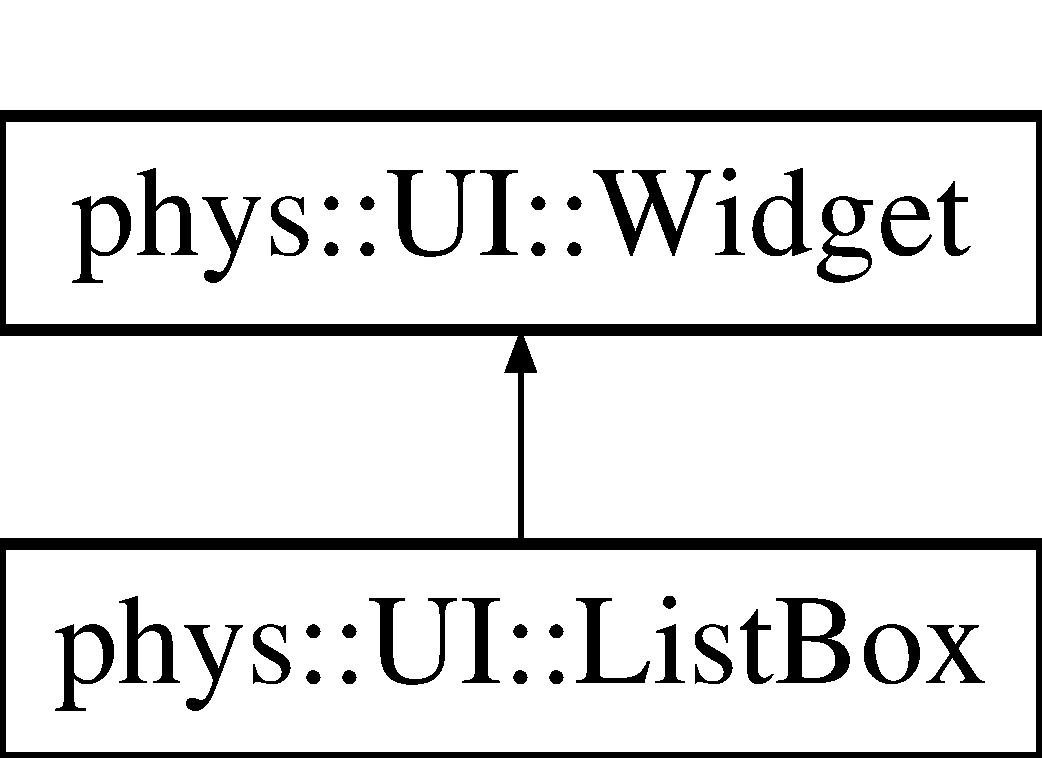
\includegraphics[height=2.000000cm]{classphys_1_1UI_1_1ListBox}
\end{center}
\end{figure}
\subsubsection*{Classes}
\begin{DoxyCompactItemize}
\item 
struct \hyperlink{structphys_1_1UI_1_1ListBox_1_1TemplateParams}{TemplateParams}
\end{DoxyCompactItemize}
\subsubsection*{Public Member Functions}
\begin{DoxyCompactItemize}
\item 
virtual \hyperlink{classphys_1_1UI_1_1Caption}{Caption} $\ast$ \hyperlink{classphys_1_1UI_1_1ListBox_aa6069fc3690e09142033886d9d7b0b3a}{AddSelection} (\hyperlink{namespacephys_a5ce5049f8b4bf88d6413c47b504ebb31}{ConstString} \&name, \hyperlink{namespacephys_a5ce5049f8b4bf88d6413c47b504ebb31}{ConstString} \&Text, \hyperlink{namespacephys_a5ce5049f8b4bf88d6413c47b504ebb31}{ConstString} \&BackgroundSprite=\char`\"{}\char`\"{})
\begin{DoxyCompactList}\small\item\em Adds a selectable caption to the list to be displayed. \item\end{DoxyCompactList}\item 
virtual bool \hyperlink{classphys_1_1UI_1_1ListBox_a789faeb98d98bb4d4d89cae8c53d4bc0}{CheckMouseHover} ()
\begin{DoxyCompactList}\small\item\em Checks to see if the current mouse position is over this List Box. \item\end{DoxyCompactList}\item 
virtual void \hyperlink{classphys_1_1UI_1_1ListBox_a295acf830ed17c78a59e5ba871a5a234}{DestroySelection} (\hyperlink{classphys_1_1UI_1_1Caption}{Caption} $\ast$ToBeDestroyed)
\begin{DoxyCompactList}\small\item\em Destroys a selectable caption. \item\end{DoxyCompactList}\item 
virtual void \hyperlink{classphys_1_1UI_1_1ListBox_a3aa3bfaee473b7590692e8707dada68d}{DestroySelection} (\hyperlink{namespacephys_aa03900411993de7fbfec4789bc1d392e}{String} \&ToBeDestroyed)
\begin{DoxyCompactList}\small\item\em Destroys a selectable caption. \item\end{DoxyCompactList}\item 
virtual \hyperlink{classphys_1_1Vector2}{Vector2} \hyperlink{classphys_1_1UI_1_1ListBox_a44046453283fb2c54e10dc868705352a}{GetActualPosition} ()
\begin{DoxyCompactList}\small\item\em Sets the pixel position of this List Box. \item\end{DoxyCompactList}\item 
virtual \hyperlink{classphys_1_1Vector2}{Vector2} \hyperlink{classphys_1_1UI_1_1ListBox_a23133ed4a98994d838acee4c6a981e04}{GetActualSize} ()
\begin{DoxyCompactList}\small\item\em Sets the pixel size of this List Box. \item\end{DoxyCompactList}\item 
virtual \hyperlink{classphys_1_1UI_1_1Rectangle}{Rectangle} $\ast$ \hyperlink{classphys_1_1UI_1_1ListBox_a087fba492ebd70a58d2772fccbfec466}{GetBoxBack} ()
\begin{DoxyCompactList}\small\item\em Gets the background of this List Box. \item\end{DoxyCompactList}\item 
virtual \hyperlink{classphys_1_1Vector2}{Vector2} \hyperlink{classphys_1_1UI_1_1ListBox_af688db0628a5588865a890584f754b02}{GetPosition} ()
\begin{DoxyCompactList}\small\item\em Gets the relative position of this List Box. \item\end{DoxyCompactList}\item 
virtual \hyperlink{classphys_1_1UI_1_1Caption}{Caption} $\ast$ \hyperlink{classphys_1_1UI_1_1ListBox_a729f4ef3e0bc10bf8e96f20a83767484}{GetSelected} ()
\begin{DoxyCompactList}\small\item\em Gets the currently selected caption. \item\end{DoxyCompactList}\item 
virtual \hyperlink{classphys_1_1UI_1_1Caption}{Caption} $\ast$ \hyperlink{classphys_1_1UI_1_1ListBox_a1a5f9c44430387cc96744411bea9e978}{GetSelection} (\hyperlink{namespacephys_a5ce5049f8b4bf88d6413c47b504ebb31}{ConstString} \&Name)
\begin{DoxyCompactList}\small\item\em Gets a caption by name. \item\end{DoxyCompactList}\item 
virtual \hyperlink{classphys_1_1Vector2}{Vector2} \hyperlink{classphys_1_1UI_1_1ListBox_a7af2cced185d63be6a62d5122c700d81}{GetSize} ()
\begin{DoxyCompactList}\small\item\em Gets the relative size of this List Box. \item\end{DoxyCompactList}\item 
virtual const \hyperlink{structphys_1_1UI_1_1ListBox_1_1TemplateParams}{ListBox::TemplateParams} \& \hyperlink{classphys_1_1UI_1_1ListBox_a138619898628207d48adfe2bb08536d8}{GetTemplateInfo} ()
\begin{DoxyCompactList}\small\item\em Gets the struct containing all the current template parameters used when creating a new selections. \item\end{DoxyCompactList}\item 
virtual \hyperlink{classphys_1_1UI_1_1Scrollbar}{UI::Scrollbar} $\ast$ \hyperlink{classphys_1_1UI_1_1ListBox_a9f62475c3a81772407af38076363060e}{GetVertScroll} ()
\begin{DoxyCompactList}\small\item\em Gets the scrollbar used within this List Box. \item\end{DoxyCompactList}\item 
\hypertarget{classphys_1_1UI_1_1ListBox_a896220f2423ce6295ea3c8dc3a10d4b8}{
virtual void \hyperlink{classphys_1_1UI_1_1ListBox_a896220f2423ce6295ea3c8dc3a10d4b8}{Hide} ()}
\label{classphys_1_1UI_1_1ListBox_a896220f2423ce6295ea3c8dc3a10d4b8}

\begin{DoxyCompactList}\small\item\em Forces this List Box to hide. \item\end{DoxyCompactList}\item 
virtual bool \hyperlink{classphys_1_1UI_1_1ListBox_a638f19eb6e5a0bd3291fab1ebaccc84f}{IsVisible} ()
\begin{DoxyCompactList}\small\item\em Gets the visibility of this List Box. \item\end{DoxyCompactList}\item 
\hyperlink{classphys_1_1UI_1_1ListBox_a2c61aa8ff40ff66eb45388a4e6cca5b2}{ListBox} (\hyperlink{namespacephys_a5ce5049f8b4bf88d6413c47b504ebb31}{ConstString} \&name, const \hyperlink{structphys_1_1UI_1_1RenderableRect}{RenderableRect} \&Rect, const UI::ScrollbarStyle \&ScrollStyle, \hyperlink{classphys_1_1UI_1_1Layer}{Layer} $\ast$PLayer)
\begin{DoxyCompactList}\small\item\em Standard initialization constructor. \item\end{DoxyCompactList}\item 
virtual void \hyperlink{classphys_1_1UI_1_1ListBox_a4bf1911c639429c783915ba8a543fec3}{SetActualPosition} (const \hyperlink{classphys_1_1Vector2}{Vector2} \&Position)
\begin{DoxyCompactList}\small\item\em Sets the pixel position of this List Box. \item\end{DoxyCompactList}\item 
virtual void \hyperlink{classphys_1_1UI_1_1ListBox_a742810da75f2b3889794498f05af8860}{SetActualSize} (const \hyperlink{classphys_1_1Vector2}{Vector2} \&Size)
\begin{DoxyCompactList}\small\item\em Sets the pixel size of this List Box. \item\end{DoxyCompactList}\item 
virtual void \hyperlink{classphys_1_1UI_1_1ListBox_a60fc5c1907df6d83217b25c2c8f15f48}{SetAutoHideScroll} (bool AutoHide)
\begin{DoxyCompactList}\small\item\em Eanbles or disables the scrollbar autohide. \item\end{DoxyCompactList}\item 
virtual void \hyperlink{classphys_1_1UI_1_1ListBox_acbc8e669d93665789453cb866996411b}{SetMaxDisplayedSelections} (const \hyperlink{namespacephys_a460f6bc24c8dd347b05e0366ae34f34a}{Whole} \&MaxSelections)
\begin{DoxyCompactList}\small\item\em Sets the maximum number of selections to display at once before the scrollbar appears. \item\end{DoxyCompactList}\item 
virtual void \hyperlink{classphys_1_1UI_1_1ListBox_a0c4c7141142caca342157ce4460b907d}{SetPosition} (const \hyperlink{classphys_1_1Vector2}{Vector2} \&Position)
\begin{DoxyCompactList}\small\item\em Sets the relative position of this List Box. \item\end{DoxyCompactList}\item 
virtual void \hyperlink{classphys_1_1UI_1_1ListBox_a2e1f6514f83be768dad7e357beb6ac98}{SetSize} (const \hyperlink{classphys_1_1Vector2}{Vector2} \&Size)
\begin{DoxyCompactList}\small\item\em Sets the relative size of this List Box. \item\end{DoxyCompactList}\item 
virtual \hyperlink{classphys_1_1UI_1_1ListBox}{ListBox} \& \hyperlink{classphys_1_1UI_1_1ListBox_a718421466aa6769b04b5e34b29e0e01b}{SetTemplateBackgroundColour} (const \hyperlink{classphys_1_1ColourValue}{ColourValue} \&BackgroundColour)
\begin{DoxyCompactList}\small\item\em Sets the background colour to be applied to all created Selections. \item\end{DoxyCompactList}\item 
virtual \hyperlink{classphys_1_1UI_1_1ListBox}{ListBox} \& \hyperlink{classphys_1_1UI_1_1ListBox_af2a439b21e1b1a4af0cc684c25109d60}{SetTemplateCursorOffset} (const \hyperlink{namespacephys_a460f6bc24c8dd347b05e0366ae34f34a}{Whole} \&Offset)
\begin{DoxyCompactList}\small\item\em Set the cursor offset to be applied to all created Selections. \item\end{DoxyCompactList}\item 
virtual \hyperlink{classphys_1_1UI_1_1ListBox}{ListBox} \& \hyperlink{classphys_1_1UI_1_1ListBox_a4bce62d1cee20950c41897e439fb3d79}{SetTemplateGlyphIndex} (const \hyperlink{namespacephys_a460f6bc24c8dd347b05e0366ae34f34a}{Whole} \&Glyph)
\begin{DoxyCompactList}\small\item\em Sets the glyph index to be applied to all created Selections. \item\end{DoxyCompactList}\item 
virtual \hyperlink{classphys_1_1UI_1_1ListBox}{ListBox} \& \hyperlink{classphys_1_1UI_1_1ListBox_a00ccdbe0b3a8da306b7346dff04792e0}{SetTemplateHorizontalAlign} (const UI::TextHorizontalAlign \&HorAlign)
\begin{DoxyCompactList}\small\item\em Sets the horizontal alignment to be applied to all created Selections. \item\end{DoxyCompactList}\item 
virtual \hyperlink{classphys_1_1UI_1_1ListBox}{ListBox} \& \hyperlink{classphys_1_1UI_1_1ListBox_abe6281a6f885be920ba540b81df3cf59}{SetTemplateSize} (const \hyperlink{classphys_1_1Vector2}{Vector2} \&Size, bool Relative=true)
\begin{DoxyCompactList}\small\item\em Sets the size to be applied to all created Selections. \item\end{DoxyCompactList}\item 
virtual \hyperlink{classphys_1_1UI_1_1ListBox}{ListBox} \& \hyperlink{classphys_1_1UI_1_1ListBox_a0106fde625c9e950f27a3e2611444359}{SetTemplateTextColour} (const \hyperlink{classphys_1_1ColourValue}{ColourValue} \&TextColour)
\begin{DoxyCompactList}\small\item\em Sets the text colour to be applied to all created Selections. \item\end{DoxyCompactList}\item 
virtual \hyperlink{classphys_1_1UI_1_1ListBox}{ListBox} \& \hyperlink{classphys_1_1UI_1_1ListBox_a160bc4d74c99f544a4339a3ba050868a}{SetTemplateTextScale} (const \hyperlink{namespacephys_af7eb897198d265b8e868f45240230d5f}{Real} \&Scale)
\begin{DoxyCompactList}\small\item\em Sets the text scale to be applied to all created Selections. \item\end{DoxyCompactList}\item 
virtual \hyperlink{classphys_1_1UI_1_1ListBox}{ListBox} \& \hyperlink{classphys_1_1UI_1_1ListBox_ab3b48e58a0049552c22aa17b7b8e8f1f}{SetTemplateVerticalAlign} (const UI::TextVerticalAlign \&VertAlign)
\begin{DoxyCompactList}\small\item\em Sets the vertical alignment to be applied to all created Selections. \item\end{DoxyCompactList}\item 
virtual void \hyperlink{classphys_1_1UI_1_1ListBox_abb3c87bf6669100296c1fa4f4913ea33}{SetVisible} (bool visible)
\begin{DoxyCompactList}\small\item\em Sets the visibility of this List Box. \item\end{DoxyCompactList}\item 
\hypertarget{classphys_1_1UI_1_1ListBox_add82890a307bc8fc984a0a029cfb88ae}{
virtual void \hyperlink{classphys_1_1UI_1_1ListBox_add82890a307bc8fc984a0a029cfb88ae}{Show} ()}
\label{classphys_1_1UI_1_1ListBox_add82890a307bc8fc984a0a029cfb88ae}

\begin{DoxyCompactList}\small\item\em Forces this List Box to be shown. \item\end{DoxyCompactList}\item 
\hypertarget{classphys_1_1UI_1_1ListBox_a582423223a2e310afc2a32c84d937502}{
virtual \hyperlink{classphys_1_1UI_1_1ListBox_a582423223a2e310afc2a32c84d937502}{$\sim$ListBox} ()}
\label{classphys_1_1UI_1_1ListBox_a582423223a2e310afc2a32c84d937502}

\begin{DoxyCompactList}\small\item\em Standard destructor. \item\end{DoxyCompactList}\end{DoxyCompactItemize}
\subsubsection*{Protected Member Functions}
\begin{DoxyCompactItemize}
\item 
\hypertarget{classphys_1_1UI_1_1ListBox_a8922aa7cdc3feb854a6c849b071fc8f6}{
virtual void \hyperlink{classphys_1_1UI_1_1ListBox_a8922aa7cdc3feb854a6c849b071fc8f6}{CalculateVisibleSelections} ()}
\label{classphys_1_1UI_1_1ListBox_a8922aa7cdc3feb854a6c849b071fc8f6}

\begin{DoxyCompactList}\small\item\em Determines how many items can be displayed in the box at once. \item\end{DoxyCompactList}\item 
\hypertarget{classphys_1_1UI_1_1ListBox_a4cc701e644aec861743ceff8bfc8793a}{
virtual void \hyperlink{classphys_1_1UI_1_1ListBox_a4cc701e644aec861743ceff8bfc8793a}{DrawList} ()}
\label{classphys_1_1UI_1_1ListBox_a4cc701e644aec861743ceff8bfc8793a}

\begin{DoxyCompactList}\small\item\em Updates the list of Visible buttons and hides the rest. \item\end{DoxyCompactList}\item 
\hypertarget{classphys_1_1UI_1_1ListBox_ac278c07a77081774369f76a4c7b12760}{
virtual void \hyperlink{classphys_1_1UI_1_1ListBox_ac278c07a77081774369f76a4c7b12760}{Update} (bool Force=false)}
\label{classphys_1_1UI_1_1ListBox_ac278c07a77081774369f76a4c7b12760}

\begin{DoxyCompactList}\small\item\em For use with widget update/automation. \item\end{DoxyCompactList}\end{DoxyCompactItemize}
\subsubsection*{Protected Attributes}
\begin{DoxyCompactItemize}
\item 
\hypertarget{classphys_1_1UI_1_1ListBox_a45271c1bffa336d7c86ce9c70b83e000}{
bool {\bfseries AutoHideScroll}}
\label{classphys_1_1UI_1_1ListBox_a45271c1bffa336d7c86ce9c70b83e000}

\item 
\hypertarget{classphys_1_1UI_1_1ListBox_a07de9457be75ad3b9ff21683d99d545b}{
\hyperlink{classphys_1_1UI_1_1Rectangle}{Rectangle} $\ast$ {\bfseries BoxBack}}
\label{classphys_1_1UI_1_1ListBox_a07de9457be75ad3b9ff21683d99d545b}

\item 
\hypertarget{classphys_1_1UI_1_1ListBox_a963c94fef825d15befd0058c70a1d2df}{
\hyperlink{classphys_1_1UI_1_1Caption}{Caption} $\ast$ {\bfseries HoveredCaption}}
\label{classphys_1_1UI_1_1ListBox_a963c94fef825d15befd0058c70a1d2df}

\item 
\hypertarget{classphys_1_1UI_1_1ListBox_a8a68a1177b1a273ada009245533a808c}{
\hyperlink{namespacephys_af7eb897198d265b8e868f45240230d5f}{Real} {\bfseries LastScrollValue}}
\label{classphys_1_1UI_1_1ListBox_a8a68a1177b1a273ada009245533a808c}

\item 
\hypertarget{classphys_1_1UI_1_1ListBox_a6a92bf3428daa9a02a7e6bf3dafd5886}{
\hyperlink{namespacephys_a460f6bc24c8dd347b05e0366ae34f34a}{Whole} {\bfseries MaxDisplay}}
\label{classphys_1_1UI_1_1ListBox_a6a92bf3428daa9a02a7e6bf3dafd5886}

\item 
\hypertarget{classphys_1_1UI_1_1ListBox_a8cab85b310d794830d381722458e1a64}{
\hyperlink{namespacephys_a460f6bc24c8dd347b05e0366ae34f34a}{Whole} {\bfseries NumVisible}}
\label{classphys_1_1UI_1_1ListBox_a8cab85b310d794830d381722458e1a64}

\item 
\hypertarget{classphys_1_1UI_1_1ListBox_a62d0841248552db1479b8be601c3a5c3}{
\hyperlink{classphys_1_1UI_1_1Caption}{Caption} $\ast$ {\bfseries Selected}}
\label{classphys_1_1UI_1_1ListBox_a62d0841248552db1479b8be601c3a5c3}

\item 
\hypertarget{classphys_1_1UI_1_1ListBox_a5a514bce001102aef65c79a0e810d11b}{
std::vector$<$ \hyperlink{classphys_1_1UI_1_1Caption}{Caption} $\ast$ $>$ {\bfseries Selections}}
\label{classphys_1_1UI_1_1ListBox_a5a514bce001102aef65c79a0e810d11b}

\item 
\hypertarget{classphys_1_1UI_1_1ListBox_a0b3eac78b1352511bb770f265c6390d1}{
\hyperlink{structphys_1_1UI_1_1ListBox_1_1TemplateParams}{TemplateParams} {\bfseries SelectionTemplate}}
\label{classphys_1_1UI_1_1ListBox_a0b3eac78b1352511bb770f265c6390d1}

\item 
\hyperlink{classphys_1_1UI_1_1Scrollbar}{UI::Scrollbar} $\ast$ \hyperlink{classphys_1_1UI_1_1ListBox_ab2b012b345ff4bb1a5b228fef88d895c}{VertScroll}
\item 
\hypertarget{classphys_1_1UI_1_1ListBox_adb069b745918dd8ea9678a0fc199bf1c}{
std::vector$<$ \hyperlink{classphys_1_1UI_1_1Caption}{Caption} $\ast$ $>$ {\bfseries VisibleSelections}}
\label{classphys_1_1UI_1_1ListBox_adb069b745918dd8ea9678a0fc199bf1c}

\end{DoxyCompactItemize}


\subsubsection{Detailed Description}
This is a widget for displaying a list of captions in a box. 

Definition at line 61 of file uilistbox.h.



\subsubsection{Constructor \& Destructor Documentation}
\hypertarget{classphys_1_1UI_1_1ListBox_a2c61aa8ff40ff66eb45388a4e6cca5b2}{
\index{phys::UI::ListBox@{phys::UI::ListBox}!ListBox@{ListBox}}
\index{ListBox@{ListBox}!phys::UI::ListBox@{phys::UI::ListBox}}
\paragraph[{ListBox}]{\setlength{\rightskip}{0pt plus 5cm}phys::UI::ListBox::ListBox (
\begin{DoxyParamCaption}
\item[{{\bf ConstString} \&}]{name, }
\item[{const {\bf RenderableRect} \&}]{Rect, }
\item[{const UI::ScrollbarStyle \&}]{ScrollStyle, }
\item[{{\bf Layer} $\ast$}]{PLayer}
\end{DoxyParamCaption}
)}\hfill}
\label{classphys_1_1UI_1_1ListBox_a2c61aa8ff40ff66eb45388a4e6cca5b2}


Standard initialization constructor. 


\begin{DoxyParams}{Parameters}
{\em name} & The name of the List Box. \\
\hline
{\em Rect} & The Rect representing the position and size of the List Box. The size portion of this rect would be in reference to the size of a single selection. The actual size of this widget will be a result of how many selections are currently being displayed. \\
\hline
{\em ScrollStyle} & The style of the scrollbar you want for this List Box. See \hyperlink{classphys_1_1UI_1_1Scrollbar}{Scrollbar} class for more information. \\
\hline
{\em \hyperlink{classphys_1_1UI_1_1Layer}{Layer}} & The parent layer this List Box belongs to. \\
\hline
\end{DoxyParams}


\begin{Desc}
\item[\hyperlink{todo__todo000027}{Todo}]Currently this class has little support for a border around the selections. Ideally when the UI system is more complete we'll be able to seemlessly move objects around different layers and thus have more control over z-\/order. When that happens we should add a rect to this class be be placed over the selections for use with a border or other kind of decoration. \end{Desc}


\begin{Desc}
\item[\hyperlink{todo__todo000028}{Todo}]Fourth instance of needing to include the namespace in the declaration seemingly needlessly. \end{Desc}




Definition at line 60 of file uilistbox.cpp.



\subsubsection{Member Function Documentation}
\hypertarget{classphys_1_1UI_1_1ListBox_aa6069fc3690e09142033886d9d7b0b3a}{
\index{phys::UI::ListBox@{phys::UI::ListBox}!AddSelection@{AddSelection}}
\index{AddSelection@{AddSelection}!phys::UI::ListBox@{phys::UI::ListBox}}
\paragraph[{AddSelection}]{\setlength{\rightskip}{0pt plus 5cm}{\bf Caption} $\ast$ phys::UI::ListBox::AddSelection (
\begin{DoxyParamCaption}
\item[{{\bf ConstString} \&}]{name, }
\item[{{\bf ConstString} \&}]{Text, }
\item[{{\bf ConstString} \&}]{BackgroundSprite = {\ttfamily \char`\"{}\char`\"{}}}
\end{DoxyParamCaption}
)\hspace{0.3cm}{\ttfamily  \mbox{[}virtual\mbox{]}}}\hfill}
\label{classphys_1_1UI_1_1ListBox_aa6069fc3690e09142033886d9d7b0b3a}


Adds a selectable caption to the list to be displayed. 

If a colour other then white was set as the template and you try to set a background sprite, it will attempt to blend the colour and sprite. Pure white colour will cause the sprite to look normal. 
\begin{DoxyParams}{Parameters}
{\em name} & A name for the selection. \\
\hline
{\em Text} & The text to be displayed within the created caption. \\
\hline
{\em BackgroundSprite} & Optional, name of the sprite to set as it's background. Ignored if the string is empty. \\
\hline
\end{DoxyParams}


Definition at line 352 of file uilistbox.cpp.

\hypertarget{classphys_1_1UI_1_1ListBox_a789faeb98d98bb4d4d89cae8c53d4bc0}{
\index{phys::UI::ListBox@{phys::UI::ListBox}!CheckMouseHover@{CheckMouseHover}}
\index{CheckMouseHover@{CheckMouseHover}!phys::UI::ListBox@{phys::UI::ListBox}}
\paragraph[{CheckMouseHover}]{\setlength{\rightskip}{0pt plus 5cm}bool phys::UI::ListBox::CheckMouseHover (
\begin{DoxyParamCaption}
{}
\end{DoxyParamCaption}
)\hspace{0.3cm}{\ttfamily  \mbox{[}virtual\mbox{]}}}\hfill}
\label{classphys_1_1UI_1_1ListBox_a789faeb98d98bb4d4d89cae8c53d4bc0}


Checks to see if the current mouse position is over this List Box. 

\begin{DoxyReturn}{Returns}
Returns a bool value, true if the mouse is over this List Box, false if it's not. 
\end{DoxyReturn}


Implements \hyperlink{classphys_1_1UI_1_1Widget_a613df6dbb42efe139d185043a00259dc}{phys::UI::Widget}.



Definition at line 268 of file uilistbox.cpp.

\hypertarget{classphys_1_1UI_1_1ListBox_a295acf830ed17c78a59e5ba871a5a234}{
\index{phys::UI::ListBox@{phys::UI::ListBox}!DestroySelection@{DestroySelection}}
\index{DestroySelection@{DestroySelection}!phys::UI::ListBox@{phys::UI::ListBox}}
\paragraph[{DestroySelection}]{\setlength{\rightskip}{0pt plus 5cm}void phys::UI::ListBox::DestroySelection (
\begin{DoxyParamCaption}
\item[{{\bf Caption} $\ast$}]{ToBeDestroyed}
\end{DoxyParamCaption}
)\hspace{0.3cm}{\ttfamily  \mbox{[}virtual\mbox{]}}}\hfill}
\label{classphys_1_1UI_1_1ListBox_a295acf830ed17c78a59e5ba871a5a234}


Destroys a selectable caption. 


\begin{DoxyParams}{Parameters}
{\em ToBeDestroyed} & A pointer to the caption you want destroyed and removed from this list. \\
\hline
\end{DoxyParams}


Definition at line 387 of file uilistbox.cpp.

\hypertarget{classphys_1_1UI_1_1ListBox_a3aa3bfaee473b7590692e8707dada68d}{
\index{phys::UI::ListBox@{phys::UI::ListBox}!DestroySelection@{DestroySelection}}
\index{DestroySelection@{DestroySelection}!phys::UI::ListBox@{phys::UI::ListBox}}
\paragraph[{DestroySelection}]{\setlength{\rightskip}{0pt plus 5cm}void phys::UI::ListBox::DestroySelection (
\begin{DoxyParamCaption}
\item[{{\bf String} \&}]{ToBeDestroyed}
\end{DoxyParamCaption}
)\hspace{0.3cm}{\ttfamily  \mbox{[}virtual\mbox{]}}}\hfill}
\label{classphys_1_1UI_1_1ListBox_a3aa3bfaee473b7590692e8707dada68d}


Destroys a selectable caption. 


\begin{DoxyParams}{Parameters}
{\em ToBeDestroyed} & A string naming the caption you want destroyed and removed from this list. \\
\hline
\end{DoxyParams}


Definition at line 401 of file uilistbox.cpp.

\hypertarget{classphys_1_1UI_1_1ListBox_a44046453283fb2c54e10dc868705352a}{
\index{phys::UI::ListBox@{phys::UI::ListBox}!GetActualPosition@{GetActualPosition}}
\index{GetActualPosition@{GetActualPosition}!phys::UI::ListBox@{phys::UI::ListBox}}
\paragraph[{GetActualPosition}]{\setlength{\rightskip}{0pt plus 5cm}{\bf Vector2} phys::UI::ListBox::GetActualPosition (
\begin{DoxyParamCaption}
{}
\end{DoxyParamCaption}
)\hspace{0.3cm}{\ttfamily  \mbox{[}virtual\mbox{]}}}\hfill}
\label{classphys_1_1UI_1_1ListBox_a44046453283fb2c54e10dc868705352a}


Sets the pixel position of this List Box. 

\begin{DoxyReturn}{Returns}
Returns a vector2 representing the pixel position of this List Box. 
\end{DoxyReturn}


Implements \hyperlink{classphys_1_1UI_1_1Widget_a0a29fecff7f56d7909f65fd63b0990e7}{phys::UI::Widget}.



Definition at line 450 of file uilistbox.cpp.

\hypertarget{classphys_1_1UI_1_1ListBox_a23133ed4a98994d838acee4c6a981e04}{
\index{phys::UI::ListBox@{phys::UI::ListBox}!GetActualSize@{GetActualSize}}
\index{GetActualSize@{GetActualSize}!phys::UI::ListBox@{phys::UI::ListBox}}
\paragraph[{GetActualSize}]{\setlength{\rightskip}{0pt plus 5cm}{\bf Vector2} phys::UI::ListBox::GetActualSize (
\begin{DoxyParamCaption}
{}
\end{DoxyParamCaption}
)\hspace{0.3cm}{\ttfamily  \mbox{[}virtual\mbox{]}}}\hfill}
\label{classphys_1_1UI_1_1ListBox_a23133ed4a98994d838acee4c6a981e04}


Sets the pixel size of this List Box. 

\begin{DoxyReturn}{Returns}
Returns a vector2 representing the pixel size of this List Box. 
\end{DoxyReturn}


Implements \hyperlink{classphys_1_1UI_1_1Widget_af3a685621ed220748c0940ea38c96ed2}{phys::UI::Widget}.



Definition at line 484 of file uilistbox.cpp.

\hypertarget{classphys_1_1UI_1_1ListBox_a087fba492ebd70a58d2772fccbfec466}{
\index{phys::UI::ListBox@{phys::UI::ListBox}!GetBoxBack@{GetBoxBack}}
\index{GetBoxBack@{GetBoxBack}!phys::UI::ListBox@{phys::UI::ListBox}}
\paragraph[{GetBoxBack}]{\setlength{\rightskip}{0pt plus 5cm}{\bf Rectangle} $\ast$ phys::UI::ListBox::GetBoxBack (
\begin{DoxyParamCaption}
{}
\end{DoxyParamCaption}
)\hspace{0.3cm}{\ttfamily  \mbox{[}virtual\mbox{]}}}\hfill}
\label{classphys_1_1UI_1_1ListBox_a087fba492ebd70a58d2772fccbfec466}


Gets the background of this List Box. 

\begin{DoxyReturn}{Returns}
Returns a pointer to the background of this List Box. 
\end{DoxyReturn}


Definition at line 494 of file uilistbox.cpp.

\hypertarget{classphys_1_1UI_1_1ListBox_af688db0628a5588865a890584f754b02}{
\index{phys::UI::ListBox@{phys::UI::ListBox}!GetPosition@{GetPosition}}
\index{GetPosition@{GetPosition}!phys::UI::ListBox@{phys::UI::ListBox}}
\paragraph[{GetPosition}]{\setlength{\rightskip}{0pt plus 5cm}{\bf Vector2} phys::UI::ListBox::GetPosition (
\begin{DoxyParamCaption}
{}
\end{DoxyParamCaption}
)\hspace{0.3cm}{\ttfamily  \mbox{[}virtual\mbox{]}}}\hfill}
\label{classphys_1_1UI_1_1ListBox_af688db0628a5588865a890584f754b02}


Gets the relative position of this List Box. 

The position is relative to the screen size. Values range from 0.0 to 1.0. \begin{DoxyReturn}{Returns}
Returns a vector2 representing the relative position of this List Box. 
\end{DoxyReturn}


Implements \hyperlink{classphys_1_1UI_1_1Widget_a3e464b028b0d1b5755923b8790260c33}{phys::UI::Widget}.



Definition at line 436 of file uilistbox.cpp.

\hypertarget{classphys_1_1UI_1_1ListBox_a729f4ef3e0bc10bf8e96f20a83767484}{
\index{phys::UI::ListBox@{phys::UI::ListBox}!GetSelected@{GetSelected}}
\index{GetSelected@{GetSelected}!phys::UI::ListBox@{phys::UI::ListBox}}
\paragraph[{GetSelected}]{\setlength{\rightskip}{0pt plus 5cm}{\bf Caption} $\ast$ phys::UI::ListBox::GetSelected (
\begin{DoxyParamCaption}
{}
\end{DoxyParamCaption}
)\hspace{0.3cm}{\ttfamily  \mbox{[}virtual\mbox{]}}}\hfill}
\label{classphys_1_1UI_1_1ListBox_a729f4ef3e0bc10bf8e96f20a83767484}


Gets the currently selected caption. 

\begin{DoxyReturn}{Returns}
Returns a pointer to the currently selected caption, or NULL if none are selected. 
\end{DoxyReturn}


Definition at line 489 of file uilistbox.cpp.

\hypertarget{classphys_1_1UI_1_1ListBox_a1a5f9c44430387cc96744411bea9e978}{
\index{phys::UI::ListBox@{phys::UI::ListBox}!GetSelection@{GetSelection}}
\index{GetSelection@{GetSelection}!phys::UI::ListBox@{phys::UI::ListBox}}
\paragraph[{GetSelection}]{\setlength{\rightskip}{0pt plus 5cm}{\bf Caption} $\ast$ phys::UI::ListBox::GetSelection (
\begin{DoxyParamCaption}
\item[{{\bf ConstString} \&}]{Name}
\end{DoxyParamCaption}
)\hspace{0.3cm}{\ttfamily  \mbox{[}virtual\mbox{]}}}\hfill}
\label{classphys_1_1UI_1_1ListBox_a1a5f9c44430387cc96744411bea9e978}


Gets a caption by name. 


\begin{DoxyParams}{Parameters}
{\em Name} & The name of the selectable caption you want to get. \\
\hline
\end{DoxyParams}
\begin{DoxyReturn}{Returns}
Returns a pointer to the named caption. 
\end{DoxyReturn}


Definition at line 374 of file uilistbox.cpp.

\hypertarget{classphys_1_1UI_1_1ListBox_a7af2cced185d63be6a62d5122c700d81}{
\index{phys::UI::ListBox@{phys::UI::ListBox}!GetSize@{GetSize}}
\index{GetSize@{GetSize}!phys::UI::ListBox@{phys::UI::ListBox}}
\paragraph[{GetSize}]{\setlength{\rightskip}{0pt plus 5cm}{\bf Vector2} phys::UI::ListBox::GetSize (
\begin{DoxyParamCaption}
{}
\end{DoxyParamCaption}
)\hspace{0.3cm}{\ttfamily  \mbox{[}virtual\mbox{]}}}\hfill}
\label{classphys_1_1UI_1_1ListBox_a7af2cced185d63be6a62d5122c700d81}


Gets the relative size of this List Box. 

The size is relative to the screen size. Values range from 0.0 to 1.0. \begin{DoxyReturn}{Returns}
Returns a vector2 representing the relative size of this List Box. 
\end{DoxyReturn}


Implements \hyperlink{classphys_1_1UI_1_1Widget_a07039c19e57de314147ce066417da0a2}{phys::UI::Widget}.



Definition at line 467 of file uilistbox.cpp.

\hypertarget{classphys_1_1UI_1_1ListBox_a138619898628207d48adfe2bb08536d8}{
\index{phys::UI::ListBox@{phys::UI::ListBox}!GetTemplateInfo@{GetTemplateInfo}}
\index{GetTemplateInfo@{GetTemplateInfo}!phys::UI::ListBox@{phys::UI::ListBox}}
\paragraph[{GetTemplateInfo}]{\setlength{\rightskip}{0pt plus 5cm}const {\bf ListBox::TemplateParams} \& phys::UI::ListBox::GetTemplateInfo (
\begin{DoxyParamCaption}
{}
\end{DoxyParamCaption}
)\hspace{0.3cm}{\ttfamily  \mbox{[}virtual\mbox{]}}}\hfill}
\label{classphys_1_1UI_1_1ListBox_a138619898628207d48adfe2bb08536d8}


Gets the struct containing all the current template parameters used when creating a new selections. 

\begin{DoxyReturn}{Returns}
Returns a const reference to the structure containing all the template parameters. 
\end{DoxyReturn}


Definition at line 347 of file uilistbox.cpp.

\hypertarget{classphys_1_1UI_1_1ListBox_a9f62475c3a81772407af38076363060e}{
\index{phys::UI::ListBox@{phys::UI::ListBox}!GetVertScroll@{GetVertScroll}}
\index{GetVertScroll@{GetVertScroll}!phys::UI::ListBox@{phys::UI::ListBox}}
\paragraph[{GetVertScroll}]{\setlength{\rightskip}{0pt plus 5cm}{\bf UI::Scrollbar} $\ast$ phys::UI::ListBox::GetVertScroll (
\begin{DoxyParamCaption}
{}
\end{DoxyParamCaption}
)\hspace{0.3cm}{\ttfamily  \mbox{[}virtual\mbox{]}}}\hfill}
\label{classphys_1_1UI_1_1ListBox_a9f62475c3a81772407af38076363060e}


Gets the scrollbar used within this List Box. 

\begin{DoxyReturn}{Returns}
Returns a pointer to the scrollbar of this List Box. 
\end{DoxyReturn}


Definition at line 499 of file uilistbox.cpp.

\hypertarget{classphys_1_1UI_1_1ListBox_a638f19eb6e5a0bd3291fab1ebaccc84f}{
\index{phys::UI::ListBox@{phys::UI::ListBox}!IsVisible@{IsVisible}}
\index{IsVisible@{IsVisible}!phys::UI::ListBox@{phys::UI::ListBox}}
\paragraph[{IsVisible}]{\setlength{\rightskip}{0pt plus 5cm}bool phys::UI::ListBox::IsVisible (
\begin{DoxyParamCaption}
{}
\end{DoxyParamCaption}
)\hspace{0.3cm}{\ttfamily  \mbox{[}virtual\mbox{]}}}\hfill}
\label{classphys_1_1UI_1_1ListBox_a638f19eb6e5a0bd3291fab1ebaccc84f}


Gets the visibility of this List Box. 

\begin{DoxyReturn}{Returns}
Returns a bool representing the visibility of this List Box. 
\end{DoxyReturn}


Implements \hyperlink{classphys_1_1UI_1_1Widget_aaf1a1bd31b8e626467ce9cdb69bdf7ac}{phys::UI::Widget}.



Definition at line 243 of file uilistbox.cpp.

\hypertarget{classphys_1_1UI_1_1ListBox_a4bf1911c639429c783915ba8a543fec3}{
\index{phys::UI::ListBox@{phys::UI::ListBox}!SetActualPosition@{SetActualPosition}}
\index{SetActualPosition@{SetActualPosition}!phys::UI::ListBox@{phys::UI::ListBox}}
\paragraph[{SetActualPosition}]{\setlength{\rightskip}{0pt plus 5cm}void phys::UI::ListBox::SetActualPosition (
\begin{DoxyParamCaption}
\item[{const {\bf Vector2} \&}]{Position}
\end{DoxyParamCaption}
)\hspace{0.3cm}{\ttfamily  \mbox{[}virtual\mbox{]}}}\hfill}
\label{classphys_1_1UI_1_1ListBox_a4bf1911c639429c783915ba8a543fec3}


Sets the pixel position of this List Box. 


\begin{DoxyParams}{Parameters}
{\em Position} & A vector2 representing the pixel position of this List Box. \\
\hline
\end{DoxyParams}


Implements \hyperlink{classphys_1_1UI_1_1Widget_a77727351d98b10f1f4eb45048cb882e3}{phys::UI::Widget}.



Definition at line 441 of file uilistbox.cpp.

\hypertarget{classphys_1_1UI_1_1ListBox_a742810da75f2b3889794498f05af8860}{
\index{phys::UI::ListBox@{phys::UI::ListBox}!SetActualSize@{SetActualSize}}
\index{SetActualSize@{SetActualSize}!phys::UI::ListBox@{phys::UI::ListBox}}
\paragraph[{SetActualSize}]{\setlength{\rightskip}{0pt plus 5cm}void phys::UI::ListBox::SetActualSize (
\begin{DoxyParamCaption}
\item[{const {\bf Vector2} \&}]{Size}
\end{DoxyParamCaption}
)\hspace{0.3cm}{\ttfamily  \mbox{[}virtual\mbox{]}}}\hfill}
\label{classphys_1_1UI_1_1ListBox_a742810da75f2b3889794498f05af8860}


Sets the pixel size of this List Box. 


\begin{DoxyParams}{Parameters}
{\em Size} & A vector2 representing the pixel size of this List Box. \\
\hline
\end{DoxyParams}


Implements \hyperlink{classphys_1_1UI_1_1Widget_acda63a62fa158d5fe00c86f50e5c120d}{phys::UI::Widget}.



Definition at line 472 of file uilistbox.cpp.

\hypertarget{classphys_1_1UI_1_1ListBox_a60fc5c1907df6d83217b25c2c8f15f48}{
\index{phys::UI::ListBox@{phys::UI::ListBox}!SetAutoHideScroll@{SetAutoHideScroll}}
\index{SetAutoHideScroll@{SetAutoHideScroll}!phys::UI::ListBox@{phys::UI::ListBox}}
\paragraph[{SetAutoHideScroll}]{\setlength{\rightskip}{0pt plus 5cm}void phys::UI::ListBox::SetAutoHideScroll (
\begin{DoxyParamCaption}
\item[{bool}]{AutoHide}
\end{DoxyParamCaption}
)\hspace{0.3cm}{\ttfamily  \mbox{[}virtual\mbox{]}}}\hfill}
\label{classphys_1_1UI_1_1ListBox_a60fc5c1907df6d83217b25c2c8f15f48}


Eanbles or disables the scrollbar autohide. 


\begin{DoxyParams}{Parameters}
{\em AutoHide} & A bool indicating whether or not to auto hide the scrollbar. \\
\hline
\end{DoxyParams}


Definition at line 420 of file uilistbox.cpp.

\hypertarget{classphys_1_1UI_1_1ListBox_acbc8e669d93665789453cb866996411b}{
\index{phys::UI::ListBox@{phys::UI::ListBox}!SetMaxDisplayedSelections@{SetMaxDisplayedSelections}}
\index{SetMaxDisplayedSelections@{SetMaxDisplayedSelections}!phys::UI::ListBox@{phys::UI::ListBox}}
\paragraph[{SetMaxDisplayedSelections}]{\setlength{\rightskip}{0pt plus 5cm}void phys::UI::ListBox::SetMaxDisplayedSelections (
\begin{DoxyParamCaption}
\item[{const {\bf Whole} \&}]{MaxSelections}
\end{DoxyParamCaption}
)\hspace{0.3cm}{\ttfamily  \mbox{[}virtual\mbox{]}}}\hfill}
\label{classphys_1_1UI_1_1ListBox_acbc8e669d93665789453cb866996411b}


Sets the maximum number of selections to display at once before the scrollbar appears. 


\begin{DoxyParams}{Parameters}
{\em MaxSelections} & The maximum number of selections to display at once before requiring a scrollbar. This indirectly controls the max size of this widget. \\
\hline
\end{DoxyParams}


Definition at line 415 of file uilistbox.cpp.

\hypertarget{classphys_1_1UI_1_1ListBox_a0c4c7141142caca342157ce4460b907d}{
\index{phys::UI::ListBox@{phys::UI::ListBox}!SetPosition@{SetPosition}}
\index{SetPosition@{SetPosition}!phys::UI::ListBox@{phys::UI::ListBox}}
\paragraph[{SetPosition}]{\setlength{\rightskip}{0pt plus 5cm}void phys::UI::ListBox::SetPosition (
\begin{DoxyParamCaption}
\item[{const {\bf Vector2} \&}]{Position}
\end{DoxyParamCaption}
)\hspace{0.3cm}{\ttfamily  \mbox{[}virtual\mbox{]}}}\hfill}
\label{classphys_1_1UI_1_1ListBox_a0c4c7141142caca342157ce4460b907d}


Sets the relative position of this List Box. 

The position is relative to the screen size. Values range from 0.0 to 1.0. 
\begin{DoxyParams}{Parameters}
{\em Position} & A vector2 representing the relative position of this List Box. \\
\hline
\end{DoxyParams}


Implements \hyperlink{classphys_1_1UI_1_1Widget_a3ef894be2c0868105b2bf495ae944d00}{phys::UI::Widget}.



Definition at line 427 of file uilistbox.cpp.

\hypertarget{classphys_1_1UI_1_1ListBox_a2e1f6514f83be768dad7e357beb6ac98}{
\index{phys::UI::ListBox@{phys::UI::ListBox}!SetSize@{SetSize}}
\index{SetSize@{SetSize}!phys::UI::ListBox@{phys::UI::ListBox}}
\paragraph[{SetSize}]{\setlength{\rightskip}{0pt plus 5cm}void phys::UI::ListBox::SetSize (
\begin{DoxyParamCaption}
\item[{const {\bf Vector2} \&}]{Size}
\end{DoxyParamCaption}
)\hspace{0.3cm}{\ttfamily  \mbox{[}virtual\mbox{]}}}\hfill}
\label{classphys_1_1UI_1_1ListBox_a2e1f6514f83be768dad7e357beb6ac98}


Sets the relative size of this List Box. 

The size is relative to the screen size. Values range from 0.0 to 1.0. 
\begin{DoxyParams}{Parameters}
{\em Size} & A vector2 representing the relative size of this List Box. \\
\hline
\end{DoxyParams}


Implements \hyperlink{classphys_1_1UI_1_1Widget_a00f73c12583d25a75c089f944075b24d}{phys::UI::Widget}.



Definition at line 455 of file uilistbox.cpp.

\hypertarget{classphys_1_1UI_1_1ListBox_a718421466aa6769b04b5e34b29e0e01b}{
\index{phys::UI::ListBox@{phys::UI::ListBox}!SetTemplateBackgroundColour@{SetTemplateBackgroundColour}}
\index{SetTemplateBackgroundColour@{SetTemplateBackgroundColour}!phys::UI::ListBox@{phys::UI::ListBox}}
\paragraph[{SetTemplateBackgroundColour}]{\setlength{\rightskip}{0pt plus 5cm}{\bf ListBox} \& phys::UI::ListBox::SetTemplateBackgroundColour (
\begin{DoxyParamCaption}
\item[{const {\bf ColourValue} \&}]{BackgroundColour}
\end{DoxyParamCaption}
)\hspace{0.3cm}{\ttfamily  \mbox{[}virtual\mbox{]}}}\hfill}
\label{classphys_1_1UI_1_1ListBox_a718421466aa6769b04b5e34b29e0e01b}


Sets the background colour to be applied to all created Selections. 

Optional parameter. 
\begin{DoxyParams}{Parameters}
{\em BackgroundColour} & The colour to set for the captions background. This defaults to white. \\
\hline
\end{DoxyParams}
\begin{DoxyReturn}{Returns}
Returns a reference to this List Box. 
\end{DoxyReturn}


Definition at line 329 of file uilistbox.cpp.

\hypertarget{classphys_1_1UI_1_1ListBox_af2a439b21e1b1a4af0cc684c25109d60}{
\index{phys::UI::ListBox@{phys::UI::ListBox}!SetTemplateCursorOffset@{SetTemplateCursorOffset}}
\index{SetTemplateCursorOffset@{SetTemplateCursorOffset}!phys::UI::ListBox@{phys::UI::ListBox}}
\paragraph[{SetTemplateCursorOffset}]{\setlength{\rightskip}{0pt plus 5cm}{\bf ListBox} \& phys::UI::ListBox::SetTemplateCursorOffset (
\begin{DoxyParamCaption}
\item[{const {\bf Whole} \&}]{Offset}
\end{DoxyParamCaption}
)\hspace{0.3cm}{\ttfamily  \mbox{[}virtual\mbox{]}}}\hfill}
\label{classphys_1_1UI_1_1ListBox_af2a439b21e1b1a4af0cc684c25109d60}


Set the cursor offset to be applied to all created Selections. 

Optional parameter. 
\begin{DoxyParams}{Parameters}
{\em Offset} & The offset in pixels to adjust where text starts appearing in the caption. \\
\hline
\end{DoxyParams}
\begin{DoxyReturn}{Returns}
Returns a reference to this List Box. 
\end{DoxyReturn}


Definition at line 323 of file uilistbox.cpp.

\hypertarget{classphys_1_1UI_1_1ListBox_a4bce62d1cee20950c41897e439fb3d79}{
\index{phys::UI::ListBox@{phys::UI::ListBox}!SetTemplateGlyphIndex@{SetTemplateGlyphIndex}}
\index{SetTemplateGlyphIndex@{SetTemplateGlyphIndex}!phys::UI::ListBox@{phys::UI::ListBox}}
\paragraph[{SetTemplateGlyphIndex}]{\setlength{\rightskip}{0pt plus 5cm}{\bf ListBox} \& phys::UI::ListBox::SetTemplateGlyphIndex (
\begin{DoxyParamCaption}
\item[{const {\bf Whole} \&}]{Glyph}
\end{DoxyParamCaption}
)\hspace{0.3cm}{\ttfamily  \mbox{[}virtual\mbox{]}}}\hfill}
\label{classphys_1_1UI_1_1ListBox_a4bce62d1cee20950c41897e439fb3d79}


Sets the glyph index to be applied to all created Selections. 

This needs to be called prior to the creation of any selections(captions). This defaults to 0, which may not be a valid font index in your gorilla file. In which case it will throw an exception. 
\begin{DoxyParams}{Parameters}
{\em Glyph} & The Glyph index to use for the text generated by all captions in this widget. \\
\hline
\end{DoxyParams}
\begin{DoxyReturn}{Returns}
Returns a reference to this List Box. 
\end{DoxyReturn}


Definition at line 305 of file uilistbox.cpp.

\hypertarget{classphys_1_1UI_1_1ListBox_a00ccdbe0b3a8da306b7346dff04792e0}{
\index{phys::UI::ListBox@{phys::UI::ListBox}!SetTemplateHorizontalAlign@{SetTemplateHorizontalAlign}}
\index{SetTemplateHorizontalAlign@{SetTemplateHorizontalAlign}!phys::UI::ListBox@{phys::UI::ListBox}}
\paragraph[{SetTemplateHorizontalAlign}]{\setlength{\rightskip}{0pt plus 5cm}{\bf ListBox} \& phys::UI::ListBox::SetTemplateHorizontalAlign (
\begin{DoxyParamCaption}
\item[{const UI::TextHorizontalAlign \&}]{HorAlign}
\end{DoxyParamCaption}
)\hspace{0.3cm}{\ttfamily  \mbox{[}virtual\mbox{]}}}\hfill}
\label{classphys_1_1UI_1_1ListBox_a00ccdbe0b3a8da306b7346dff04792e0}


Sets the horizontal alignment to be applied to all created Selections. 

Optional parameter. 
\begin{DoxyParams}{Parameters}
{\em HorAlign} & The horizontal text alignment. This defaults to UI::Middle. \\
\hline
\end{DoxyParams}
\begin{DoxyReturn}{Returns}
Returns a reference to this List Box. 
\end{DoxyReturn}


Definition at line 335 of file uilistbox.cpp.

\hypertarget{classphys_1_1UI_1_1ListBox_abe6281a6f885be920ba540b81df3cf59}{
\index{phys::UI::ListBox@{phys::UI::ListBox}!SetTemplateSize@{SetTemplateSize}}
\index{SetTemplateSize@{SetTemplateSize}!phys::UI::ListBox@{phys::UI::ListBox}}
\paragraph[{SetTemplateSize}]{\setlength{\rightskip}{0pt plus 5cm}{\bf ListBox} \& phys::UI::ListBox::SetTemplateSize (
\begin{DoxyParamCaption}
\item[{const {\bf Vector2} \&}]{Size, }
\item[{bool}]{Relative = {\ttfamily true}}
\end{DoxyParamCaption}
)\hspace{0.3cm}{\ttfamily  \mbox{[}virtual\mbox{]}}}\hfill}
\label{classphys_1_1UI_1_1ListBox_abe6281a6f885be920ba540b81df3cf59}


Sets the size to be applied to all created Selections. 


\begin{DoxyParams}{Parameters}
{\em Size} & The size of the caption to make. Applied to all captions created by this class. \\
\hline
{\em Relative} & Whether or not the size provided is in relative units(rather then pixels). \\
\hline
\end{DoxyParams}
\begin{DoxyReturn}{Returns}
Returns a reference to this List Box. 
\end{DoxyReturn}


Definition at line 298 of file uilistbox.cpp.

\hypertarget{classphys_1_1UI_1_1ListBox_a0106fde625c9e950f27a3e2611444359}{
\index{phys::UI::ListBox@{phys::UI::ListBox}!SetTemplateTextColour@{SetTemplateTextColour}}
\index{SetTemplateTextColour@{SetTemplateTextColour}!phys::UI::ListBox@{phys::UI::ListBox}}
\paragraph[{SetTemplateTextColour}]{\setlength{\rightskip}{0pt plus 5cm}{\bf ListBox} \& phys::UI::ListBox::SetTemplateTextColour (
\begin{DoxyParamCaption}
\item[{const {\bf ColourValue} \&}]{TextColour}
\end{DoxyParamCaption}
)\hspace{0.3cm}{\ttfamily  \mbox{[}virtual\mbox{]}}}\hfill}
\label{classphys_1_1UI_1_1ListBox_a0106fde625c9e950f27a3e2611444359}


Sets the text colour to be applied to all created Selections. 

Optional parameter. 
\begin{DoxyParams}{Parameters}
{\em TextColour} & The Colour of the text. This defaults to black. \\
\hline
\end{DoxyParams}
\begin{DoxyReturn}{Returns}
Returns a reference to this List Box. 
\end{DoxyReturn}


Definition at line 311 of file uilistbox.cpp.

\hypertarget{classphys_1_1UI_1_1ListBox_a160bc4d74c99f544a4339a3ba050868a}{
\index{phys::UI::ListBox@{phys::UI::ListBox}!SetTemplateTextScale@{SetTemplateTextScale}}
\index{SetTemplateTextScale@{SetTemplateTextScale}!phys::UI::ListBox@{phys::UI::ListBox}}
\paragraph[{SetTemplateTextScale}]{\setlength{\rightskip}{0pt plus 5cm}{\bf ListBox} \& phys::UI::ListBox::SetTemplateTextScale (
\begin{DoxyParamCaption}
\item[{const {\bf Real} \&}]{Scale}
\end{DoxyParamCaption}
)\hspace{0.3cm}{\ttfamily  \mbox{[}virtual\mbox{]}}}\hfill}
\label{classphys_1_1UI_1_1ListBox_a160bc4d74c99f544a4339a3ba050868a}


Sets the text scale to be applied to all created Selections. 

Optional parameter. 
\begin{DoxyParams}{Parameters}
{\em Scale} & The scale you wish to apply to the text in all created selections. \\
\hline
\end{DoxyParams}
\begin{DoxyReturn}{Returns}
Returns a reference to this List Box. 
\end{DoxyReturn}


Definition at line 317 of file uilistbox.cpp.

\hypertarget{classphys_1_1UI_1_1ListBox_ab3b48e58a0049552c22aa17b7b8e8f1f}{
\index{phys::UI::ListBox@{phys::UI::ListBox}!SetTemplateVerticalAlign@{SetTemplateVerticalAlign}}
\index{SetTemplateVerticalAlign@{SetTemplateVerticalAlign}!phys::UI::ListBox@{phys::UI::ListBox}}
\paragraph[{SetTemplateVerticalAlign}]{\setlength{\rightskip}{0pt plus 5cm}{\bf ListBox} \& phys::UI::ListBox::SetTemplateVerticalAlign (
\begin{DoxyParamCaption}
\item[{const UI::TextVerticalAlign \&}]{VertAlign}
\end{DoxyParamCaption}
)\hspace{0.3cm}{\ttfamily  \mbox{[}virtual\mbox{]}}}\hfill}
\label{classphys_1_1UI_1_1ListBox_ab3b48e58a0049552c22aa17b7b8e8f1f}


Sets the vertical alignment to be applied to all created Selections. 

Optional parameter. 
\begin{DoxyParams}{Parameters}
{\em VertAlign} & The Vertical text alignment. This defaults to UI::Center. \\
\hline
\end{DoxyParams}
\begin{DoxyReturn}{Returns}
Returns a reference to this List Box. 
\end{DoxyReturn}


Definition at line 341 of file uilistbox.cpp.

\hypertarget{classphys_1_1UI_1_1ListBox_abb3c87bf6669100296c1fa4f4913ea33}{
\index{phys::UI::ListBox@{phys::UI::ListBox}!SetVisible@{SetVisible}}
\index{SetVisible@{SetVisible}!phys::UI::ListBox@{phys::UI::ListBox}}
\paragraph[{SetVisible}]{\setlength{\rightskip}{0pt plus 5cm}void phys::UI::ListBox::SetVisible (
\begin{DoxyParamCaption}
\item[{bool}]{visible}
\end{DoxyParamCaption}
)\hspace{0.3cm}{\ttfamily  \mbox{[}virtual\mbox{]}}}\hfill}
\label{classphys_1_1UI_1_1ListBox_abb3c87bf6669100296c1fa4f4913ea33}


Sets the visibility of this List Box. 


\begin{DoxyParams}{Parameters}
{\em visible} & Bool determining whether or not this List Box should be visible. \\
\hline
\end{DoxyParams}


Implements \hyperlink{classphys_1_1UI_1_1Widget_ab049233d8d5522a6ab42654b8924a3e0}{phys::UI::Widget}.



Definition at line 233 of file uilistbox.cpp.



\subsubsection{Member Data Documentation}
\hypertarget{classphys_1_1UI_1_1ListBox_ab2b012b345ff4bb1a5b228fef88d895c}{
\index{phys::UI::ListBox@{phys::UI::ListBox}!VertScroll@{VertScroll}}
\index{VertScroll@{VertScroll}!phys::UI::ListBox@{phys::UI::ListBox}}
\paragraph[{VertScroll}]{\setlength{\rightskip}{0pt plus 5cm}{\bf UI::Scrollbar}$\ast$ {\bf phys::UI::ListBox::VertScroll}\hspace{0.3cm}{\ttfamily  \mbox{[}protected\mbox{]}}}\hfill}
\label{classphys_1_1UI_1_1ListBox_ab2b012b345ff4bb1a5b228fef88d895c}
\begin{Desc}
\item[\hyperlink{todo__todo000029}{Todo}]Third instance of needing to include the namespace in the declaration seemingly needlessly. \end{Desc}


Definition at line 78 of file uilistbox.h.



The documentation for this class was generated from the following files:\begin{DoxyCompactItemize}
\item 
uilistbox.h\item 
uilistbox.cpp\end{DoxyCompactItemize}

\hypertarget{classphys_1_1ManagerBase}{
\section{phys::ManagerBase Class Reference}
\label{d2/de3/classphys_1_1ManagerBase}\index{phys::ManagerBase@{phys::ManagerBase}}
}


This is the base class from which all the \hyperlink{classphys_1_1World}{World} Managers inherit.  




{\ttfamily \#include $<$managerbase.h$>$}

Inheritance diagram for phys::ManagerBase:\begin{figure}[H]
\begin{center}
\leavevmode
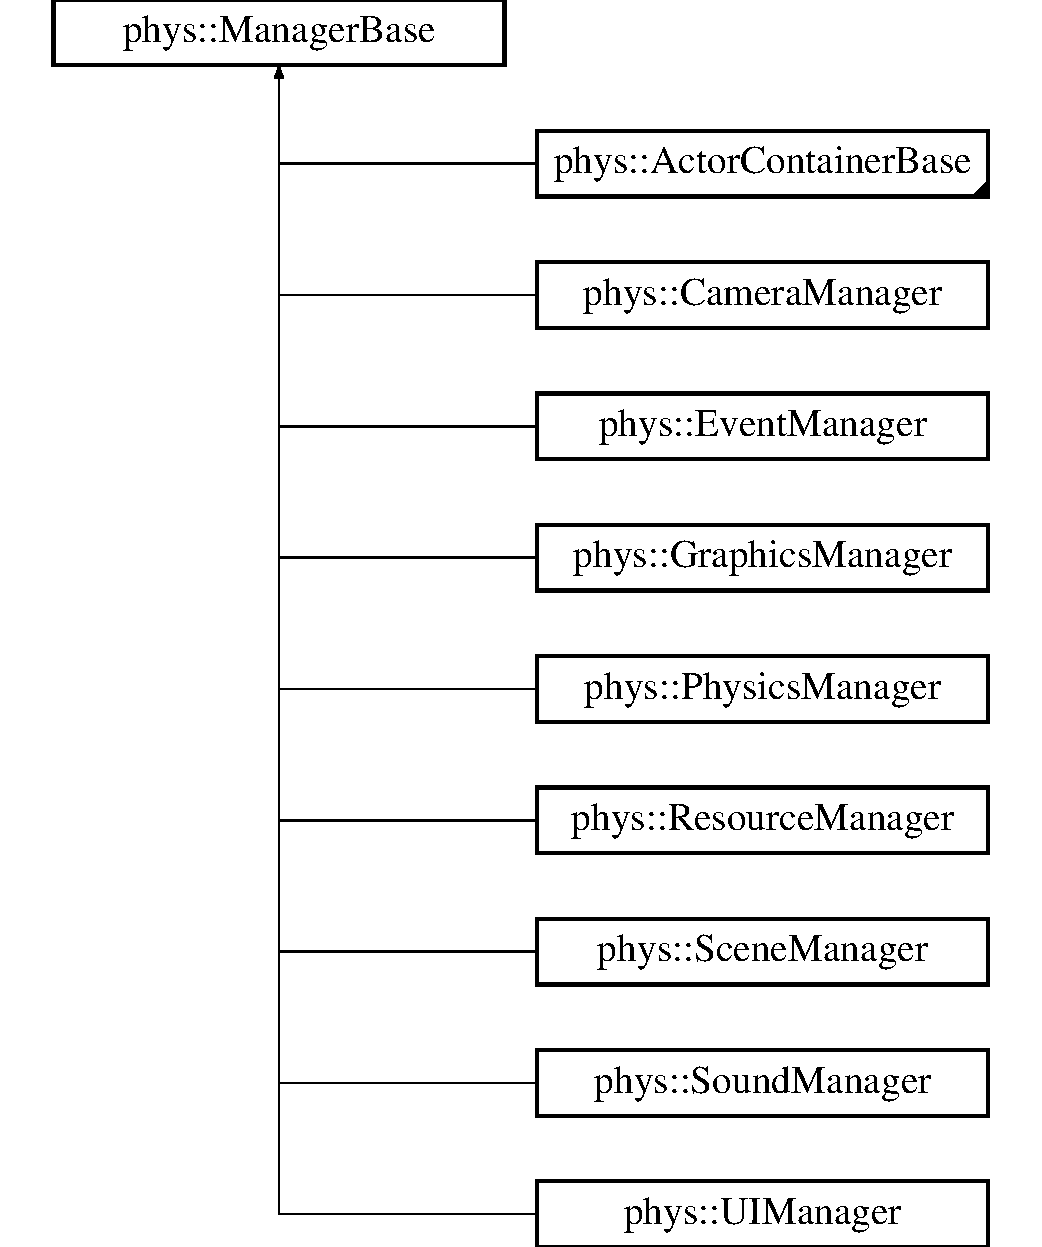
\includegraphics[height=10cm]{d2/de3/classphys_1_1ManagerBase}
\end{center}
\end{figure}
\subsection*{Public Types}
\begin{DoxyCompactItemize}
\item 
enum \hyperlink{classphys_1_1ManagerBase_aaa6ccddf23892eaccb898529414f80a5}{ManagerTypeName} \{ \par
{\bfseries ActorContainerBase}, 
{\bfseries CameraManager}, 
{\bfseries EventManager}, 
{\bfseries GraphicsManager}, 
\par
{\bfseries PhysicsManager}, 
{\bfseries ResourceManager}, 
{\bfseries SceneManager}, 
{\bfseries SoundManager}, 
\par
{\bfseries UIManager}, 
\hyperlink{classphys_1_1ManagerBase_aaa6ccddf23892eaccb898529414f80a5a3239296e554feede76c4bcb6f824c66c}{UserCreated}
 \}
\begin{DoxyCompactList}\small\item\em A listing of Manager TypeNames. \item\end{DoxyCompactList}\item 
\hypertarget{classphys_1_1ManagerBase_a753f5f0127131529767beab2502f480b}{
typedef bool($\ast$ \hyperlink{classphys_1_1ManagerBase_a753f5f0127131529767beab2502f480b}{Callback} )()}
\label{d2/de3/classphys_1_1ManagerBase_a753f5f0127131529767beab2502f480b}

\begin{DoxyCompactList}\small\item\em This makes working with Callback function pointer a bit easier. \item\end{DoxyCompactList}\end{DoxyCompactItemize}
\subsection*{Public Member Functions}
\begin{DoxyCompactItemize}
\item 
\hyperlink{classphys_1_1ManagerBase_a80c0d01d0dc19511cd08fc6ac805a616}{ManagerBase} ()
\begin{DoxyCompactList}\small\item\em Default Constructor. \item\end{DoxyCompactList}\item 
\hyperlink{classphys_1_1ManagerBase_ab9ad12416f771d95fe8a6d953923c634}{ManagerBase} (\hyperlink{classphys_1_1World}{World} $\ast$GameWorld\_\-)
\begin{DoxyCompactList}\small\item\em Simple Constructor. \item\end{DoxyCompactList}\item 
virtual \hyperlink{classphys_1_1ManagerBase_a802dace8381459637297e9a372bfdf0c}{$\sim$ManagerBase} ()
\begin{DoxyCompactList}\small\item\em Deconstructor. \item\end{DoxyCompactList}\item 
virtual void \hyperlink{classphys_1_1ManagerBase_a57dd8e54e767427d5bdcc86dc66d73ed}{Initialize} ()=0
\begin{DoxyCompactList}\small\item\em Configure Items requiring other Managers. \item\end{DoxyCompactList}\item 
virtual \hyperlink{classphys_1_1World}{World} $\ast$ \hyperlink{classphys_1_1ManagerBase_addfd62fbc444ca4c2aba40768d1b284e}{GetGameWorld} () const 
\begin{DoxyCompactList}\small\item\em This gets the \hyperlink{classphys_1_1World}{World} that this manager is working with. \item\end{DoxyCompactList}\item 
virtual void \hyperlink{classphys_1_1ManagerBase_a97eb1e77c1f7a0925fc623836368a262}{SetGameWorld} (\hyperlink{classphys_1_1World}{World} $\ast$GameWorld\_\-)
\begin{DoxyCompactList}\small\item\em This sets the \hyperlink{classphys_1_1World}{phys::World} that this Manager works with. \item\end{DoxyCompactList}\item 
virtual \hyperlink{classphys_1_1ManagerBase_aaa6ccddf23892eaccb898529414f80a5}{ManagerTypeName} \hyperlink{classphys_1_1ManagerBase_aff400b6599db635e24796d8221e9a0e3}{GetType} () const =0
\begin{DoxyCompactList}\small\item\em This returns the type of this manager. \item\end{DoxyCompactList}\item 
virtual void \hyperlink{classphys_1_1ManagerBase_a3fcf207a451d0047f884babadd0bc53e}{SetPreMainLoopItems} (\hyperlink{classphys_1_1ManagerBase_a753f5f0127131529767beab2502f480b}{Callback} PreMainCallback)
\begin{DoxyCompactList}\small\item\em This assigns a function to be the callback function to run prior to the main loop. \item\end{DoxyCompactList}\item 
virtual bool \hyperlink{classphys_1_1ManagerBase_af6210834a8af592481cf6aefa9916d88}{PreMainLoopItems} ()
\begin{DoxyCompactList}\small\item\em This runs any callback that is required before the mainloop items are run. \item\end{DoxyCompactList}\item 
virtual \hyperlink{classphys_1_1ManagerBase_a753f5f0127131529767beab2502f480b}{Callback} \hyperlink{classphys_1_1ManagerBase_a02a92b0d5df8b8b877822bdf57ec8ffc}{GetPreMainLoopItems} () const 
\begin{DoxyCompactList}\small\item\em This returns the Callback that would be called before the main loop items. \item\end{DoxyCompactList}\item 
\hypertarget{classphys_1_1ManagerBase_aa068aefaf902c87dc641b463ac93ff36}{
virtual void \hyperlink{classphys_1_1ManagerBase_aa068aefaf902c87dc641b463ac93ff36}{ErasePreMainLoopItems} ()}
\label{d2/de3/classphys_1_1ManagerBase_aa068aefaf902c87dc641b463ac93ff36}

\begin{DoxyCompactList}\small\item\em This simply calls \hyperlink{classphys_1_1ManagerBase_a3fcf207a451d0047f884babadd0bc53e}{SetPreMainLoopItems()} passing it 0. \item\end{DoxyCompactList}\item 
virtual void \hyperlink{classphys_1_1ManagerBase_aa9e13a3f7c398b708f0f242610b5abf7}{DoMainLoopItems} ()=0
\begin{DoxyCompactList}\small\item\em The main loop calls this once per frame. \item\end{DoxyCompactList}\item 
virtual void \hyperlink{classphys_1_1ManagerBase_a673b3adef73c467f4d90514a5133bf7c}{SetPostMainLoopItems} (\hyperlink{classphys_1_1ManagerBase_a753f5f0127131529767beab2502f480b}{Callback} PostMainCallback)
\begin{DoxyCompactList}\small\item\em This assigns a function to be the callback function to run prior to the main loop. \item\end{DoxyCompactList}\item 
virtual bool \hyperlink{classphys_1_1ManagerBase_afc3572602f96bdeb8215c386ff870820}{PostMainLoopItems} ()
\begin{DoxyCompactList}\small\item\em This runs any callback that is required after the mainloop items are run. \item\end{DoxyCompactList}\item 
virtual \hyperlink{classphys_1_1ManagerBase_a753f5f0127131529767beab2502f480b}{Callback} \hyperlink{classphys_1_1ManagerBase_a1e541b261e5747ebcfcefdd3dcff78ce}{GetPostMainLoopItems} () const 
\begin{DoxyCompactList}\small\item\em This returns the Callback that would be called before the main loop items. \item\end{DoxyCompactList}\item 
\hypertarget{classphys_1_1ManagerBase_a9306dafe9ffe52916b84cf157fbc12d8}{
virtual void \hyperlink{classphys_1_1ManagerBase_a9306dafe9ffe52916b84cf157fbc12d8}{ErasePostMainLoopItems} ()}
\label{d2/de3/classphys_1_1ManagerBase_a9306dafe9ffe52916b84cf157fbc12d8}

\begin{DoxyCompactList}\small\item\em This simply calls \hyperlink{classphys_1_1ManagerBase_a673b3adef73c467f4d90514a5133bf7c}{SetPostMainLoopItems()} passing it 0. \item\end{DoxyCompactList}\item 
virtual short int \hyperlink{classphys_1_1ManagerBase_af1798db3b808a658bdf14d8914d9b91d}{GetPriority} ()
\begin{DoxyCompactList}\small\item\em This gets the Priority of this manager. \item\end{DoxyCompactList}\item 
virtual void \hyperlink{classphys_1_1ManagerBase_a6e30dc5f2a9c64f95efb2ef4428b0f98}{SetPriority} (short int Priority\_\-)
\begin{DoxyCompactList}\small\item\em This gets the Priority of this manager. \item\end{DoxyCompactList}\item 
std::string \hyperlink{classphys_1_1ManagerBase_a5b4c1105696b868b7858c59541af4756}{GetTypeName} ()
\begin{DoxyCompactList}\small\item\em This Allows any manager to be sent to a stream. Primarily used for logging. \item\end{DoxyCompactList}\end{DoxyCompactItemize}
\subsection*{Protected Attributes}
\begin{DoxyCompactItemize}
\item 
\hyperlink{classphys_1_1World}{World} $\ast$ \hyperlink{classphys_1_1ManagerBase_ae2f158b4b2fef1bf2bee2524e0236c7b}{GameWorld}
\begin{DoxyCompactList}\small\item\em The actual pointer to the world. \item\end{DoxyCompactList}\item 
\hyperlink{classphys_1_1ManagerBase_a753f5f0127131529767beab2502f480b}{Callback} \hyperlink{classphys_1_1ManagerBase_a93eb2f1a30d913a4e99180b0965eb5db}{PreMainLoop}
\begin{DoxyCompactList}\small\item\em This is a function pointer to the function that should be called before running Main Loop Items. \item\end{DoxyCompactList}\item 
\hyperlink{classphys_1_1ManagerBase_a753f5f0127131529767beab2502f480b}{Callback} \hyperlink{classphys_1_1ManagerBase_aa1e80a30f151c07e06d1f4650f315da5}{PostMainLoop}
\begin{DoxyCompactList}\small\item\em This is a function pointer to the function that should be called after running Main Loop Items. \item\end{DoxyCompactList}\item 
short int \hyperlink{classphys_1_1ManagerBase_a28e2690fbcf644a7780a53b81821d8ef}{Priority}
\begin{DoxyCompactList}\small\item\em This is a weighting used by the main loop to decide what order the managers should be called in. \item\end{DoxyCompactList}\end{DoxyCompactItemize}


\subsection{Detailed Description}
This is the base class from which all the \hyperlink{classphys_1_1World}{World} Managers inherit. This creates a base set of functions that Managers are all expected to implement. 

Definition at line 57 of file managerbase.h.



\subsection{Member Enumeration Documentation}
\hypertarget{classphys_1_1ManagerBase_aaa6ccddf23892eaccb898529414f80a5}{
\index{phys::ManagerBase@{phys::ManagerBase}!ManagerTypeName@{ManagerTypeName}}
\index{ManagerTypeName@{ManagerTypeName}!phys::ManagerBase@{phys::ManagerBase}}
\subsubsection[{ManagerTypeName}]{\setlength{\rightskip}{0pt plus 5cm}enum {\bf phys::ManagerBase::ManagerTypeName}}}
\label{d2/de3/classphys_1_1ManagerBase_aaa6ccddf23892eaccb898529414f80a5}


A listing of Manager TypeNames. 

These will be returned by \hyperlink{classphys_1_1ManagerBase_aff400b6599db635e24796d8221e9a0e3}{ManagerBase::GetType()}, and will allow code using this to determine what type of Manager class they are working with and use this information to more safely cast to the correct manager if needed. \begin{Desc}
\item[Enumerator: ]\par
\begin{description}
\index{UserCreated@{UserCreated}!phys::ManagerBase@{phys::ManagerBase}}\index{phys::ManagerBase@{phys::ManagerBase}!UserCreated@{UserCreated}}\item[{\em 
\hypertarget{classphys_1_1ManagerBase_aaa6ccddf23892eaccb898529414f80a5a3239296e554feede76c4bcb6f824c66c}{
UserCreated}
\label{d2/de3/classphys_1_1ManagerBase_aaa6ccddf23892eaccb898529414f80a5a3239296e554feede76c4bcb6f824c66c}
}]This is what User created managers that do not derive from any other managers are expected to use to prevent confusion with game internals. \end{description}
\end{Desc}



Definition at line 65 of file managerbase.h.



\subsection{Constructor \& Destructor Documentation}
\hypertarget{classphys_1_1ManagerBase_a80c0d01d0dc19511cd08fc6ac805a616}{
\index{phys::ManagerBase@{phys::ManagerBase}!ManagerBase@{ManagerBase}}
\index{ManagerBase@{ManagerBase}!phys::ManagerBase@{phys::ManagerBase}}
\subsubsection[{ManagerBase}]{\setlength{\rightskip}{0pt plus 5cm}phys::ManagerBase::ManagerBase ()}}
\label{d2/de3/classphys_1_1ManagerBase_a80c0d01d0dc19511cd08fc6ac805a616}


Default Constructor. 

This creates a default manager without a valid reference to the game world. The lack of such a reference could cause issues or change behavior of a Manager class. A Manager Must be given the pointer to the world it is suppposed to work with prior to the calling of \hyperlink{classphys_1_1ManagerBase_a57dd8e54e767427d5bdcc86dc66d73ed}{ManagerBase::Initialize()}. This will most likely be the constructor used when creating a Manager to pass into the constructor of a new \hyperlink{classphys_1_1World}{phys::World}. 

Definition at line 48 of file managerbase.cpp.

\hypertarget{classphys_1_1ManagerBase_ab9ad12416f771d95fe8a6d953923c634}{
\index{phys::ManagerBase@{phys::ManagerBase}!ManagerBase@{ManagerBase}}
\index{ManagerBase@{ManagerBase}!phys::ManagerBase@{phys::ManagerBase}}
\subsubsection[{ManagerBase}]{\setlength{\rightskip}{0pt plus 5cm}phys::ManagerBase::ManagerBase ({\bf World} $\ast$ {\em GameWorld\_\-})}}
\label{d2/de3/classphys_1_1ManagerBase_ab9ad12416f771d95fe8a6d953923c634}


Simple Constructor. 

This is the prefered constructor. This is used to \char`\"{}Attach\char`\"{} a manager to a phys::world. This is expected to configure everything that this manager will need except for items requiring integration with other managers. 
\begin{DoxyParams}{Parameters}
\item[{\em GameWorld\_\-}]This is the \hyperlink{classphys_1_1World}{phys::World} this Manager is expected to work with. \end{DoxyParams}


Definition at line 56 of file managerbase.cpp.

\hypertarget{classphys_1_1ManagerBase_a802dace8381459637297e9a372bfdf0c}{
\index{phys::ManagerBase@{phys::ManagerBase}!$\sim$ManagerBase@{$\sim$ManagerBase}}
\index{$\sim$ManagerBase@{$\sim$ManagerBase}!phys::ManagerBase@{phys::ManagerBase}}
\subsubsection[{$\sim$ManagerBase}]{\setlength{\rightskip}{0pt plus 5cm}phys::ManagerBase::$\sim$ManagerBase ()\hspace{0.3cm}{\ttfamily  \mbox{[}virtual\mbox{]}}}}
\label{d2/de3/classphys_1_1ManagerBase_a802dace8381459637297e9a372bfdf0c}


Deconstructor. 

This is actuall 

Definition at line 70 of file managerbase.cpp.



\subsection{Member Function Documentation}
\hypertarget{classphys_1_1ManagerBase_aa9e13a3f7c398b708f0f242610b5abf7}{
\index{phys::ManagerBase@{phys::ManagerBase}!DoMainLoopItems@{DoMainLoopItems}}
\index{DoMainLoopItems@{DoMainLoopItems}!phys::ManagerBase@{phys::ManagerBase}}
\subsubsection[{DoMainLoopItems}]{\setlength{\rightskip}{0pt plus 5cm}virtual void phys::ManagerBase::DoMainLoopItems ()\hspace{0.3cm}{\ttfamily  \mbox{[}pure virtual\mbox{]}}}}
\label{d2/de3/classphys_1_1ManagerBase_aa9e13a3f7c398b708f0f242610b5abf7}


The main loop calls this once per frame. 

This is where each manager is expected to put anything that needs to be run each iteration of the main loop 

Implemented in \hyperlink{classphys_1_1ActorContainerBase_a67fbde6a61602253f66fecd0416bdc2f}{phys::ActorContainerBase}, \hyperlink{classphys_1_1ActorContainerVector_a883e59ac1674421bac143088a6cf07c8}{phys::ActorContainerVector}, \hyperlink{classphys_1_1CameraManager_aaae22266bccc43f6efa66d2735d7d1d3}{phys::CameraManager}, \hyperlink{classphys_1_1EventManager_aca8fb3d285484dcdb943824bf11f3596}{phys::EventManager}, \hyperlink{classphys_1_1GraphicsManager_a72e5dc563c6947cded348f19d3df41ee}{phys::GraphicsManager}, \hyperlink{classphys_1_1PhysicsManager_a62741a2582ac9bfd0255cf8a3ad2310c}{phys::PhysicsManager}, \hyperlink{classphys_1_1ResourceManager_a2114714999441c095bc28d3673c2490e}{phys::ResourceManager}, \hyperlink{classphys_1_1SceneManager_a27a3f6b21e15f628642b1cad524f1a18}{phys::SceneManager}, \hyperlink{classphys_1_1SoundManager_a577b228753ea19856b8476ab831e547e}{phys::SoundManager}, and \hyperlink{classphys_1_1UIManager_a972abedcd4343dc5966580f2f82494a8}{phys::UIManager}.

\hypertarget{classphys_1_1ManagerBase_addfd62fbc444ca4c2aba40768d1b284e}{
\index{phys::ManagerBase@{phys::ManagerBase}!GetGameWorld@{GetGameWorld}}
\index{GetGameWorld@{GetGameWorld}!phys::ManagerBase@{phys::ManagerBase}}
\subsubsection[{GetGameWorld}]{\setlength{\rightskip}{0pt plus 5cm}{\bf World} $\ast$ phys::ManagerBase::GetGameWorld () const\hspace{0.3cm}{\ttfamily  \mbox{[}virtual\mbox{]}}}}
\label{d2/de3/classphys_1_1ManagerBase_addfd62fbc444ca4c2aba40768d1b284e}


This gets the \hyperlink{classphys_1_1World}{World} that this manager is working with. 

\begin{DoxyReturn}{Returns}
This returns a \hyperlink{classphys_1_1World}{phys::World}$\ast$ that is the same as the one store in this Manager 
\end{DoxyReturn}


Reimplemented in \hyperlink{classphys_1_1ActorContainerBase_a479e6c7434f2611b0cfe6ca1fd4ebdd1}{phys::ActorContainerBase}, and \hyperlink{classphys_1_1ActorContainerVector_a5519eb0000073a2f397e158bfc368349}{phys::ActorContainerVector}.



Definition at line 64 of file managerbase.cpp.

\hypertarget{classphys_1_1ManagerBase_a1e541b261e5747ebcfcefdd3dcff78ce}{
\index{phys::ManagerBase@{phys::ManagerBase}!GetPostMainLoopItems@{GetPostMainLoopItems}}
\index{GetPostMainLoopItems@{GetPostMainLoopItems}!phys::ManagerBase@{phys::ManagerBase}}
\subsubsection[{GetPostMainLoopItems}]{\setlength{\rightskip}{0pt plus 5cm}{\bf ManagerBase::Callback} phys::ManagerBase::GetPostMainLoopItems () const\hspace{0.3cm}{\ttfamily  \mbox{[}virtual\mbox{]}}}}
\label{d2/de3/classphys_1_1ManagerBase_a1e541b261e5747ebcfcefdd3dcff78ce}


This returns the Callback that would be called before the main loop items. 

\begin{DoxyReturn}{Returns}
This returns a \hyperlink{classphys_1_1ManagerBase_a753f5f0127131529767beab2502f480b}{ManagerBase::Callback} which is a p ointer to the callback function that will be called after the main loop items 
\end{DoxyReturn}


Definition at line 104 of file managerbase.cpp.

\hypertarget{classphys_1_1ManagerBase_a02a92b0d5df8b8b877822bdf57ec8ffc}{
\index{phys::ManagerBase@{phys::ManagerBase}!GetPreMainLoopItems@{GetPreMainLoopItems}}
\index{GetPreMainLoopItems@{GetPreMainLoopItems}!phys::ManagerBase@{phys::ManagerBase}}
\subsubsection[{GetPreMainLoopItems}]{\setlength{\rightskip}{0pt plus 5cm}{\bf ManagerBase::Callback} phys::ManagerBase::GetPreMainLoopItems () const\hspace{0.3cm}{\ttfamily  \mbox{[}virtual\mbox{]}}}}
\label{d2/de3/classphys_1_1ManagerBase_a02a92b0d5df8b8b877822bdf57ec8ffc}


This returns the Callback that would be called before the main loop items. 

\begin{DoxyReturn}{Returns}
This returns a \hyperlink{classphys_1_1ManagerBase_a753f5f0127131529767beab2502f480b}{ManagerBase::Callback} which is a pointer to the callback function that will be called before the main loop items 
\end{DoxyReturn}


Definition at line 85 of file managerbase.cpp.

\hypertarget{classphys_1_1ManagerBase_af1798db3b808a658bdf14d8914d9b91d}{
\index{phys::ManagerBase@{phys::ManagerBase}!GetPriority@{GetPriority}}
\index{GetPriority@{GetPriority}!phys::ManagerBase@{phys::ManagerBase}}
\subsubsection[{GetPriority}]{\setlength{\rightskip}{0pt plus 5cm}short int phys::ManagerBase::GetPriority ()\hspace{0.3cm}{\ttfamily  \mbox{[}virtual\mbox{]}}}}
\label{d2/de3/classphys_1_1ManagerBase_af1798db3b808a658bdf14d8914d9b91d}


This gets the Priority of this manager. 

This has no Set counterpart to allow the changing of a manager's priority. This is expected to be set by the manager, or expose a safe method to change it at that level. \begin{DoxyReturn}{Returns}
This returns a short int that represents the priority of the manager. Lower is executed first. 
\end{DoxyReturn}


Definition at line 144 of file managerbase.cpp.

\hypertarget{classphys_1_1ManagerBase_aff400b6599db635e24796d8221e9a0e3}{
\index{phys::ManagerBase@{phys::ManagerBase}!GetType@{GetType}}
\index{GetType@{GetType}!phys::ManagerBase@{phys::ManagerBase}}
\subsubsection[{GetType}]{\setlength{\rightskip}{0pt plus 5cm}virtual {\bf ManagerTypeName} phys::ManagerBase::GetType () const\hspace{0.3cm}{\ttfamily  \mbox{[}pure virtual\mbox{]}}}}
\label{d2/de3/classphys_1_1ManagerBase_aff400b6599db635e24796d8221e9a0e3}


This returns the type of this manager. 

This is intended to make using and casting from Manager base easier. With this is is possible to cast from \hyperlink{classphys_1_1ManagerBase}{ManagerBase} to the correct Manager Type. \begin{DoxyReturn}{Returns}
This returns a ManagerTypeName to identify what this can be safely cast to. 
\end{DoxyReturn}


Implemented in \hyperlink{classphys_1_1ActorContainerBase_aa86380fd1b18d660f68b60f075967cf8}{phys::ActorContainerBase}, \hyperlink{classphys_1_1CameraManager_a8412ea634307aa280b615a3cc7c9b739}{phys::CameraManager}, \hyperlink{classphys_1_1EventManager_a194890f7f8be5d45aa98623481482696}{phys::EventManager}, \hyperlink{classphys_1_1GraphicsManager_abf48faad2e09cd564442e66bc0473e58}{phys::GraphicsManager}, \hyperlink{classphys_1_1PhysicsManager_a4d151cd24052ef3cccde6b66b8745be6}{phys::PhysicsManager}, \hyperlink{classphys_1_1ResourceManager_a9e5468e5428f5c108c7b3c01e94eba46}{phys::ResourceManager}, \hyperlink{classphys_1_1SceneManager_af2b4f6bc50d40ffe06f6172c3d1dd02d}{phys::SceneManager}, \hyperlink{classphys_1_1SoundManager_a6815f78a6170b119e2d1d24e862ffbf8}{phys::SoundManager}, and \hyperlink{classphys_1_1UIManager_ab8fe74564ca5dc09cbe4b1cc2c007e79}{phys::UIManager}.

\hypertarget{classphys_1_1ManagerBase_a5b4c1105696b868b7858c59541af4756}{
\index{phys::ManagerBase@{phys::ManagerBase}!GetTypeName@{GetTypeName}}
\index{GetTypeName@{GetTypeName}!phys::ManagerBase@{phys::ManagerBase}}
\subsubsection[{GetTypeName}]{\setlength{\rightskip}{0pt plus 5cm}std::string phys::ManagerBase::GetTypeName ()}}
\label{d2/de3/classphys_1_1ManagerBase_a5b4c1105696b868b7858c59541af4756}


This Allows any manager to be sent to a stream. Primarily used for logging. 

\begin{DoxyReturn}{Returns}
This returns a std::ostream\& that contains the name, and maybe some data for the the streammed manager. 
\end{DoxyReturn}


Definition at line 110 of file managerbase.cpp.

\hypertarget{classphys_1_1ManagerBase_a57dd8e54e767427d5bdcc86dc66d73ed}{
\index{phys::ManagerBase@{phys::ManagerBase}!Initialize@{Initialize}}
\index{Initialize@{Initialize}!phys::ManagerBase@{phys::ManagerBase}}
\subsubsection[{Initialize}]{\setlength{\rightskip}{0pt plus 5cm}virtual void phys::ManagerBase::Initialize ()\hspace{0.3cm}{\ttfamily  \mbox{[}pure virtual\mbox{]}}}}
\label{d2/de3/classphys_1_1ManagerBase_a57dd8e54e767427d5bdcc86dc66d73ed}


Configure Items requiring other Managers. 

If you are using the \hyperlink{classphys_1_1World}{phys::World} this is called when \hyperlink{classphys_1_1World_a21cc36be08a61f40619584d4c438936b}{phys::World::GameInit()} is called. It is expected that by the time this is called either \hyperlink{classphys_1_1ManagerBase_ab9ad12416f771d95fe8a6d953923c634}{ManagerBase::ManagerBase(World$\ast$)} or \hyperlink{classphys_1_1ManagerBase_a97eb1e77c1f7a0925fc623836368a262}{ManagerBase::SetGameWorld(World$\ast$)} will have been called. This is where all configuration that requires atleast one other manager on the \hyperlink{classphys_1_1World}{phys::World} to exist.\par
\par
 Yes we know it is spelled wrong, but are Zs cooler anyway. 

Implemented in \hyperlink{classphys_1_1ActorContainerBase_af36d5866e0ee9f6f450a4e62642e0928}{phys::ActorContainerBase}, \hyperlink{classphys_1_1ActorContainerVector_adcebf4329a587669f74e1eacc1e6912c}{phys::ActorContainerVector}, \hyperlink{classphys_1_1CameraManager_a5e956b61fa341ae576d8d160da518488}{phys::CameraManager}, \hyperlink{classphys_1_1EventManager_a51afdd83f44f461dfac5c9eca5883ea0}{phys::EventManager}, \hyperlink{classphys_1_1GraphicsManager_a554572de5d1cdce37aa1760d6e6e039c}{phys::GraphicsManager}, \hyperlink{classphys_1_1PhysicsManager_a28885be750bb763d957f122593815388}{phys::PhysicsManager}, \hyperlink{classphys_1_1ResourceManager_a9be3250f1f1153c9e079f82736eb00a8}{phys::ResourceManager}, \hyperlink{classphys_1_1SceneManager_aa13b380a4e38f706a1977237fc4b165e}{phys::SceneManager}, \hyperlink{classphys_1_1SoundManager_ae6d3957f965b54e06ec540e903cec68d}{phys::SoundManager}, and \hyperlink{classphys_1_1UIManager_af04e60c4f09c114ec3bf32babdb64ab7}{phys::UIManager}.

\hypertarget{classphys_1_1ManagerBase_afc3572602f96bdeb8215c386ff870820}{
\index{phys::ManagerBase@{phys::ManagerBase}!PostMainLoopItems@{PostMainLoopItems}}
\index{PostMainLoopItems@{PostMainLoopItems}!phys::ManagerBase@{phys::ManagerBase}}
\subsubsection[{PostMainLoopItems}]{\setlength{\rightskip}{0pt plus 5cm}bool phys::ManagerBase::PostMainLoopItems ()\hspace{0.3cm}{\ttfamily  \mbox{[}virtual\mbox{]}}}}
\label{d2/de3/classphys_1_1ManagerBase_afc3572602f96bdeb8215c386ff870820}


This runs any callback that is required after the mainloop items are run. 

This will return whatever the callback returns, which is true to end the main loop after this frame, or true to continue it. If no callback is set this simply returns true, as to not interupt the mainloop. \par
 This is a great Function to override in Manager classes where the complexity of callbacks is not required. This would make coding items that need to be performed at specific times easier. If you do that, it would be a good idea to call this version of the function, just in case a callback is set. \begin{DoxyReturn}{Returns}
This returns a false to end the main loop, or a true if the main loop should continue. 
\end{DoxyReturn}


Reimplemented in \hyperlink{classphys_1_1GraphicsManager_ae2330172be150cd4d12aa2ed62b0474c}{phys::GraphicsManager}.



Definition at line 95 of file managerbase.cpp.

\hypertarget{classphys_1_1ManagerBase_af6210834a8af592481cf6aefa9916d88}{
\index{phys::ManagerBase@{phys::ManagerBase}!PreMainLoopItems@{PreMainLoopItems}}
\index{PreMainLoopItems@{PreMainLoopItems}!phys::ManagerBase@{phys::ManagerBase}}
\subsubsection[{PreMainLoopItems}]{\setlength{\rightskip}{0pt plus 5cm}bool phys::ManagerBase::PreMainLoopItems ()\hspace{0.3cm}{\ttfamily  \mbox{[}virtual\mbox{]}}}}
\label{d2/de3/classphys_1_1ManagerBase_af6210834a8af592481cf6aefa9916d88}


This runs any callback that is required before the mainloop items are run. 

This will return whatever the callback returns, which is true to end the main loop after this frame, or true to continue it. If no callback is set this simply returns true, as to not interupt the mainloop. \par
 This is a great Function to override in Manager classes where the complexity of callbacks is not required. This would make coding items that need to be performed at specific times easier. If you do that, it would be a good idea to call this version of the function, just in case a callback is set. \begin{DoxyReturn}{Returns}
This returns a false to end the main loop, or a true if the main loop should continue. 
\end{DoxyReturn}


Definition at line 76 of file managerbase.cpp.

\hypertarget{classphys_1_1ManagerBase_a97eb1e77c1f7a0925fc623836368a262}{
\index{phys::ManagerBase@{phys::ManagerBase}!SetGameWorld@{SetGameWorld}}
\index{SetGameWorld@{SetGameWorld}!phys::ManagerBase@{phys::ManagerBase}}
\subsubsection[{SetGameWorld}]{\setlength{\rightskip}{0pt plus 5cm}void phys::ManagerBase::SetGameWorld ({\bf World} $\ast$ {\em GameWorld\_\-})\hspace{0.3cm}{\ttfamily  \mbox{[}virtual\mbox{]}}}}
\label{d2/de3/classphys_1_1ManagerBase_a97eb1e77c1f7a0925fc623836368a262}


This sets the \hyperlink{classphys_1_1World}{phys::World} that this Manager works with. 

It is expected that this won't change very much, and for some managers changing this at the wrong time could cause some very fundamental problems. In fact, managers should be designed so that they can swapped out. For example swapping out event managers could allow for a swift re-\/mapping of game controls when a game switches modes.\par
\par
 For managers that can be moved it is expected that this function will change the pointer on the \hyperlink{classphys_1_1World}{phys::World} for the appropriate manager to point to this manager. This simplifies the calls that will naturally come next. To detach a Manager from the world pass this method a NULL pointer. If the manager cannot be removed or detached it should throw and exception using \hyperlink{classphys_1_1World_a88e6bdee6b972111b6804ca746738c50}{World::LogAndThrow}, and it must not fail to attach to a world (that means it must internally handle all exception raised by the attaching process or throw an \char`\"{}Unrecoverable Error\char`\"{}) 

Reimplemented in \hyperlink{classphys_1_1ActorContainerBase_ae0cb5c288f17507247dd98d3a2466876}{phys::ActorContainerBase}, and \hyperlink{classphys_1_1ActorContainerVector_ab4c1394254057465f7a2f89b87dc49aa}{phys::ActorContainerVector}.



Definition at line 67 of file managerbase.cpp.

\hypertarget{classphys_1_1ManagerBase_a673b3adef73c467f4d90514a5133bf7c}{
\index{phys::ManagerBase@{phys::ManagerBase}!SetPostMainLoopItems@{SetPostMainLoopItems}}
\index{SetPostMainLoopItems@{SetPostMainLoopItems}!phys::ManagerBase@{phys::ManagerBase}}
\subsubsection[{SetPostMainLoopItems}]{\setlength{\rightskip}{0pt plus 5cm}void phys::ManagerBase::SetPostMainLoopItems ({\bf ManagerBase::Callback} {\em PostMainCallback})\hspace{0.3cm}{\ttfamily  \mbox{[}virtual\mbox{]}}}}
\label{d2/de3/classphys_1_1ManagerBase_a673b3adef73c467f4d90514a5133bf7c}


This assigns a function to be the callback function to run prior to the main loop. 


\begin{DoxyParams}{Parameters}
\item[{\em PostMainCallback}]This is a pointer to a function that returns a bool and accepts no arguments, this is in the form of a \hyperlink{classphys_1_1ManagerBase_a753f5f0127131529767beab2502f480b}{ManagerBase::Callback}. If SetPosMainLoopItems is passed 0, NULL or a null pointer, the callback will be forgetten and will not attempt to be called. \end{DoxyParams}


Definition at line 92 of file managerbase.cpp.

\hypertarget{classphys_1_1ManagerBase_a3fcf207a451d0047f884babadd0bc53e}{
\index{phys::ManagerBase@{phys::ManagerBase}!SetPreMainLoopItems@{SetPreMainLoopItems}}
\index{SetPreMainLoopItems@{SetPreMainLoopItems}!phys::ManagerBase@{phys::ManagerBase}}
\subsubsection[{SetPreMainLoopItems}]{\setlength{\rightskip}{0pt plus 5cm}void phys::ManagerBase::SetPreMainLoopItems ({\bf ManagerBase::Callback} {\em PreMainCallback})\hspace{0.3cm}{\ttfamily  \mbox{[}virtual\mbox{]}}}}
\label{d2/de3/classphys_1_1ManagerBase_a3fcf207a451d0047f884babadd0bc53e}


This assigns a function to be the callback function to run prior to the main loop. 


\begin{DoxyParams}{Parameters}
\item[{\em PreMainCallback}]This is a pointer to a function that returns a bool and accepts no arguments, this is in the form of a \hyperlink{classphys_1_1ManagerBase_a753f5f0127131529767beab2502f480b}{ManagerBase::Callback}. If SetPreMainLoopItems is passed 0, NULL or a null pointer, the callback will be forgetten and will not attempt to be called. \end{DoxyParams}


Definition at line 73 of file managerbase.cpp.

\hypertarget{classphys_1_1ManagerBase_a6e30dc5f2a9c64f95efb2ef4428b0f98}{
\index{phys::ManagerBase@{phys::ManagerBase}!SetPriority@{SetPriority}}
\index{SetPriority@{SetPriority}!phys::ManagerBase@{phys::ManagerBase}}
\subsubsection[{SetPriority}]{\setlength{\rightskip}{0pt plus 5cm}void phys::ManagerBase::SetPriority (short int {\em Priority\_\-})\hspace{0.3cm}{\ttfamily  \mbox{[}virtual\mbox{]}}}}
\label{d2/de3/classphys_1_1ManagerBase_a6e30dc5f2a9c64f95efb2ef4428b0f98}


This gets the Priority of this manager. 

This has no Set counterpart to allow the changing of a manager's priority. This is expected to be set by the manager, or expose a safe method to change it at that level. \begin{DoxyReturn}{Returns}
This returns a short int that represents the priority of the manager. Lower is executed first. 
\end{DoxyReturn}


Definition at line 149 of file managerbase.cpp.



\subsection{Member Data Documentation}
\hypertarget{classphys_1_1ManagerBase_ae2f158b4b2fef1bf2bee2524e0236c7b}{
\index{phys::ManagerBase@{phys::ManagerBase}!GameWorld@{GameWorld}}
\index{GameWorld@{GameWorld}!phys::ManagerBase@{phys::ManagerBase}}
\subsubsection[{GameWorld}]{\setlength{\rightskip}{0pt plus 5cm}{\bf World}$\ast$ {\bf phys::ManagerBase::GameWorld}\hspace{0.3cm}{\ttfamily  \mbox{[}protected\mbox{]}}}}
\label{d2/de3/classphys_1_1ManagerBase_ae2f158b4b2fef1bf2bee2524e0236c7b}


The actual pointer to the world. 

\begin{DoxyInternal}{For internal use only.}
\end{DoxyInternal}


Definition at line 201 of file managerbase.h.

\hypertarget{classphys_1_1ManagerBase_aa1e80a30f151c07e06d1f4650f315da5}{
\index{phys::ManagerBase@{phys::ManagerBase}!PostMainLoop@{PostMainLoop}}
\index{PostMainLoop@{PostMainLoop}!phys::ManagerBase@{phys::ManagerBase}}
\subsubsection[{PostMainLoop}]{\setlength{\rightskip}{0pt plus 5cm}{\bf Callback} {\bf phys::ManagerBase::PostMainLoop}\hspace{0.3cm}{\ttfamily  \mbox{[}protected\mbox{]}}}}
\label{d2/de3/classphys_1_1ManagerBase_aa1e80a30f151c07e06d1f4650f315da5}


This is a function pointer to the function that should be called after running Main Loop Items. 

\begin{DoxyInternal}{For internal use only.}
\end{DoxyInternal}


Definition at line 209 of file managerbase.h.

\hypertarget{classphys_1_1ManagerBase_a93eb2f1a30d913a4e99180b0965eb5db}{
\index{phys::ManagerBase@{phys::ManagerBase}!PreMainLoop@{PreMainLoop}}
\index{PreMainLoop@{PreMainLoop}!phys::ManagerBase@{phys::ManagerBase}}
\subsubsection[{PreMainLoop}]{\setlength{\rightskip}{0pt plus 5cm}{\bf Callback} {\bf phys::ManagerBase::PreMainLoop}\hspace{0.3cm}{\ttfamily  \mbox{[}protected\mbox{]}}}}
\label{d2/de3/classphys_1_1ManagerBase_a93eb2f1a30d913a4e99180b0965eb5db}


This is a function pointer to the function that should be called before running Main Loop Items. 

\begin{DoxyInternal}{For internal use only.}
\end{DoxyInternal}


Definition at line 205 of file managerbase.h.

\hypertarget{classphys_1_1ManagerBase_a28e2690fbcf644a7780a53b81821d8ef}{
\index{phys::ManagerBase@{phys::ManagerBase}!Priority@{Priority}}
\index{Priority@{Priority}!phys::ManagerBase@{phys::ManagerBase}}
\subsubsection[{Priority}]{\setlength{\rightskip}{0pt plus 5cm}short int {\bf phys::ManagerBase::Priority}\hspace{0.3cm}{\ttfamily  \mbox{[}protected\mbox{]}}}}
\label{d2/de3/classphys_1_1ManagerBase_a28e2690fbcf644a7780a53b81821d8ef}


This is a weighting used by the main loop to decide what order the managers should be called in. 

A lower number gets called earlier in the Main loop. By default rendering the graphics occurs at priority 0. 

Definition at line 214 of file managerbase.h.



The documentation for this class was generated from the following files:\begin{DoxyCompactItemize}
\item 
managerbase.h\item 
managerbase.cpp\end{DoxyCompactItemize}

\hypertarget{classphys_1_1UI_1_1MarkupText}{
\section{phys::UI::MarkupText Class Reference}
\label{d7/d23/classphys_1_1UI_1_1MarkupText}\index{phys::UI::MarkupText@{phys::UI::MarkupText}}
}


This is a helper class for use with specialized text display.  




{\ttfamily \#include $<$uimarkuptext.h$>$}

\subsection*{Public Member Functions}
\begin{DoxyCompactItemize}
\item 
\hyperlink{classphys_1_1UI_1_1MarkupText_adc462bb1d0f8220ab309ef0844b6ebd5}{MarkupText} (\hyperlink{namespacephys_a5ce5049f8b4bf88d6413c47b504ebb31}{ConstString} \&name, const \hyperlink{classphys_1_1Vector2}{Vector2} Position, const \hyperlink{namespacephys_a460f6bc24c8dd347b05e0366ae34f34a}{Whole} Glyph, \hyperlink{namespacephys_aa03900411993de7fbfec4789bc1d392e}{String} Text, \hyperlink{classphys_1_1UILayer}{UILayer} $\ast$Layer)
\begin{DoxyCompactList}\small\item\em Internal constructor. \item\end{DoxyCompactList}\item 
\hypertarget{classphys_1_1UI_1_1MarkupText_a7c5d8033801123c938089ef9ca647f01}{
virtual \hyperlink{classphys_1_1UI_1_1MarkupText_a7c5d8033801123c938089ef9ca647f01}{$\sim$MarkupText} ()}
\label{d7/d23/classphys_1_1UI_1_1MarkupText_a7c5d8033801123c938089ef9ca647f01}

\begin{DoxyCompactList}\small\item\em Class destructor. \item\end{DoxyCompactList}\item 
virtual void \hyperlink{classphys_1_1UI_1_1MarkupText_ac5c38c21af2fbc3533697cacfec8fdc3}{SetVisible} (bool Visible)
\begin{DoxyCompactList}\small\item\em Sets the visibility of this markup text. \item\end{DoxyCompactList}\item 
virtual bool \hyperlink{classphys_1_1UI_1_1MarkupText_a17873359c7387926c7e759665ad4312d}{IsVisible} ()
\begin{DoxyCompactList}\small\item\em Gets the visibility of this markup text. \item\end{DoxyCompactList}\item 
\hypertarget{classphys_1_1UI_1_1MarkupText_a223df1155960fd6a4ddde7a43e87fa09}{
virtual void \hyperlink{classphys_1_1UI_1_1MarkupText_a223df1155960fd6a4ddde7a43e87fa09}{Show} ()}
\label{d7/d23/classphys_1_1UI_1_1MarkupText_a223df1155960fd6a4ddde7a43e87fa09}

\begin{DoxyCompactList}\small\item\em Forces this markup text to be shown. \item\end{DoxyCompactList}\item 
\hypertarget{classphys_1_1UI_1_1MarkupText_ad0a4b1d27341426d08d367c4891c23f9}{
virtual void \hyperlink{classphys_1_1UI_1_1MarkupText_ad0a4b1d27341426d08d367c4891c23f9}{Hide} ()}
\label{d7/d23/classphys_1_1UI_1_1MarkupText_ad0a4b1d27341426d08d367c4891c23f9}

\begin{DoxyCompactList}\small\item\em Forces this markup text to hide. \item\end{DoxyCompactList}\item 
virtual \hyperlink{namespacephys_aa03900411993de7fbfec4789bc1d392e}{String} \& \hyperlink{classphys_1_1UI_1_1MarkupText_afa64067f890466ad4844c4836e7667fd}{GetName} ()
\begin{DoxyCompactList}\small\item\em Gets the name of this markup text. \item\end{DoxyCompactList}\item 
virtual void \hyperlink{classphys_1_1UI_1_1MarkupText_af5d9184959b56996e9727e2d7ccf8f22}{SetText} (\hyperlink{namespacephys_aa03900411993de7fbfec4789bc1d392e}{String} \&Text)
\begin{DoxyCompactList}\small\item\em Sets the text displayed within the markup text. \item\end{DoxyCompactList}\item 
virtual \hyperlink{namespacephys_aa03900411993de7fbfec4789bc1d392e}{String} \hyperlink{classphys_1_1UI_1_1MarkupText_af5d8a7e6ca03e15fc488608c28a54c1e}{GetText} ()
\begin{DoxyCompactList}\small\item\em Gets the text displayed within the markup text. \item\end{DoxyCompactList}\item 
virtual void \hyperlink{classphys_1_1UI_1_1MarkupText_ad5840b9cb7235381ce105762008326a6}{SetTextScale} (\hyperlink{namespacephys_af7eb897198d265b8e868f45240230d5f}{Real} Scale)
\begin{DoxyCompactList}\small\item\em Sets the scaling to be applied to the text being rendered. \item\end{DoxyCompactList}\item 
virtual \hyperlink{namespacephys_af7eb897198d265b8e868f45240230d5f}{Real} \hyperlink{classphys_1_1UI_1_1MarkupText_aa69d77428171e0c49c51a5d1854ffaff}{GetTextScale} ()
\begin{DoxyCompactList}\small\item\em Gets the scaling currently being applied to the rendered text. \item\end{DoxyCompactList}\item 
virtual void \hyperlink{classphys_1_1UI_1_1MarkupText_a6f0b087fca1b75a5005652ccd31a77a1}{SetDefaultGlyphIndex} (const \hyperlink{namespacephys_a460f6bc24c8dd347b05e0366ae34f34a}{Whole} DefaultGlyphIndex)
\begin{DoxyCompactList}\small\item\em Sets the Default glyph index to be used with this markup text. \item\end{DoxyCompactList}\item 
virtual \hyperlink{namespacephys_a460f6bc24c8dd347b05e0366ae34f34a}{Whole} \hyperlink{classphys_1_1UI_1_1MarkupText_a02872d0b9828b34e9b2ceec82cce237b}{GetDefaultGlyphIndex} ()
\begin{DoxyCompactList}\small\item\em Gets the Default glyph index in use by this markup text. \item\end{DoxyCompactList}\item 
virtual void \hyperlink{classphys_1_1UI_1_1MarkupText_aa4a71db4811506968086105e3126731c}{SetPosition} (const \hyperlink{classphys_1_1Vector2}{Vector2} Position)
\begin{DoxyCompactList}\small\item\em Sets the relative top left position of this markup text. \item\end{DoxyCompactList}\item 
virtual \hyperlink{classphys_1_1Vector2}{Vector2} \hyperlink{classphys_1_1UI_1_1MarkupText_a9d92f03e1cad181a5d8f20f3f95cf7cc}{GetPosition} ()
\begin{DoxyCompactList}\small\item\em Gets the relative top left position of this markup text. \item\end{DoxyCompactList}\item 
virtual void \hyperlink{classphys_1_1UI_1_1MarkupText_a0b6e052e1b592b66bc7fd923f975b7ef}{SetActualPosition} (const \hyperlink{classphys_1_1Vector2}{Vector2} Position)
\begin{DoxyCompactList}\small\item\em Sets the top left position of this markup text in pixels. \item\end{DoxyCompactList}\item 
virtual \hyperlink{classphys_1_1Vector2}{Vector2} \hyperlink{classphys_1_1UI_1_1MarkupText_a1e5bfba8d1686cb4188793fd695c7090}{GetActualPosition} ()
\begin{DoxyCompactList}\small\item\em Gets the top left position of this markup text in pixels. \item\end{DoxyCompactList}\item 
virtual void \hyperlink{classphys_1_1UI_1_1MarkupText_af8dd68edd25e9553fe559ad46852cd71}{SetMaxSize} (const \hyperlink{classphys_1_1Vector2}{Vector2} Size)
\begin{DoxyCompactList}\small\item\em Sets the maximum relative size of this markup text. \item\end{DoxyCompactList}\item 
virtual \hyperlink{classphys_1_1Vector2}{Vector2} \hyperlink{classphys_1_1UI_1_1MarkupText_ae68fd261f2dc9494a16e3089c7a35b8a}{GetMaxSize} ()
\begin{DoxyCompactList}\small\item\em Gets the maximum relative size of this markup text. \item\end{DoxyCompactList}\item 
virtual void \hyperlink{classphys_1_1UI_1_1MarkupText_a03b0e586c48e885b9c57968413603fa9}{SetMaxActualSize} (const \hyperlink{classphys_1_1Vector2}{Vector2} Size)
\begin{DoxyCompactList}\small\item\em Sets the maximum size of this markup text in pixels. \item\end{DoxyCompactList}\item 
virtual \hyperlink{classphys_1_1Vector2}{Vector2} \hyperlink{classphys_1_1UI_1_1MarkupText_a4a742f4d64038ded68c5480f4cf3e017}{GetMaxActualSize} ()
\begin{DoxyCompactList}\small\item\em Gets the maximum size of this markup text in pixels. \item\end{DoxyCompactList}\item 
virtual void \hyperlink{classphys_1_1UI_1_1MarkupText_a65662c49802fa5b82a04ac387b55493f}{SetRenderPriority} (UI::RenderPriority Priority)
\begin{DoxyCompactList}\small\item\em Sets the priority this markup text should be rendered with. \item\end{DoxyCompactList}\item 
virtual UI::RenderPriority \hyperlink{classphys_1_1UI_1_1MarkupText_a86afb23309534d86ed9675170b321874}{GetRenderPriority} ()
\begin{DoxyCompactList}\small\item\em Gets the priority this markup text should be rendered with. \item\end{DoxyCompactList}\end{DoxyCompactItemize}
\subsection*{Protected Attributes}
\begin{DoxyCompactItemize}
\item 
\hypertarget{classphys_1_1UI_1_1MarkupText_a620d8d94f82242d452776e90f3b01982}{
Gorilla::MarkupText $\ast$ {\bfseries GMarkup}}
\label{d7/d23/classphys_1_1UI_1_1MarkupText_a620d8d94f82242d452776e90f3b01982}

\item 
\hypertarget{classphys_1_1UI_1_1MarkupText_afe6c68ba31cf4861abe562d8385c4382}{
\hyperlink{classphys_1_1UILayer}{UILayer} $\ast$ {\bfseries Parent}}
\label{d7/d23/classphys_1_1UI_1_1MarkupText_afe6c68ba31cf4861abe562d8385c4382}

\item 
\hypertarget{classphys_1_1UI_1_1MarkupText_a0c2c2d00a0cc3fc18929996ca8469efe}{
\hyperlink{classphys_1_1UIManager}{UIManager} $\ast$ {\bfseries Manager}}
\label{d7/d23/classphys_1_1UI_1_1MarkupText_a0c2c2d00a0cc3fc18929996ca8469efe}

\item 
\hypertarget{classphys_1_1UI_1_1MarkupText_abbb2984fb489b7470e04b6e5c9dc0217}{
\hyperlink{namespacephys_a460f6bc24c8dd347b05e0366ae34f34a}{Whole} {\bfseries Glyphs}}
\label{d7/d23/classphys_1_1UI_1_1MarkupText_abbb2984fb489b7470e04b6e5c9dc0217}

\item 
\hypertarget{classphys_1_1UI_1_1MarkupText_af4fce680f510b38537f7b1db0eda8598}{
\hyperlink{classphys_1_1Vector2}{Vector2} {\bfseries RelPosition}}
\label{d7/d23/classphys_1_1UI_1_1MarkupText_af4fce680f510b38537f7b1db0eda8598}

\item 
\hypertarget{classphys_1_1UI_1_1MarkupText_a184fb78af719fb52fcf0408501738cdc}{
\hyperlink{classphys_1_1Vector2}{Vector2} {\bfseries RelSize}}
\label{d7/d23/classphys_1_1UI_1_1MarkupText_a184fb78af719fb52fcf0408501738cdc}

\item 
\hypertarget{classphys_1_1UI_1_1MarkupText_ab56e816bda785c058f9440e7aebd52cb}{
\hyperlink{namespacephys_aa03900411993de7fbfec4789bc1d392e}{String} {\bfseries Name}}
\label{d7/d23/classphys_1_1UI_1_1MarkupText_ab56e816bda785c058f9440e7aebd52cb}

\end{DoxyCompactItemize}


\subsection{Detailed Description}
This is a helper class for use with specialized text display. Markup Texts and Captions are similar in that they both display text messages that can be altered readily, the primary difference between the two is that Captions are meant for small simple messages with background functionality built in, where as Markup Texts have no background functionality, but they use a light markup language to accomplish special effects with the text. 

Definition at line 69 of file uimarkuptext.h.



\subsection{Constructor \& Destructor Documentation}
\hypertarget{classphys_1_1UI_1_1MarkupText_adc462bb1d0f8220ab309ef0844b6ebd5}{
\index{phys::UI::MarkupText@{phys::UI::MarkupText}!MarkupText@{MarkupText}}
\index{MarkupText@{MarkupText}!phys::UI::MarkupText@{phys::UI::MarkupText}}
\subsubsection[{MarkupText}]{\setlength{\rightskip}{0pt plus 5cm}phys::UI::MarkupText::MarkupText (
\begin{DoxyParamCaption}
\item[{{\bf ConstString} \&}]{ name, }
\item[{const {\bf Vector2}}]{ Position, }
\item[{const {\bf Whole}}]{ Glyph, }
\item[{{\bf String}}]{ Text, }
\item[{{\bf UILayer} $\ast$}]{ Layer}
\end{DoxyParamCaption}
)}}
\label{d7/d23/classphys_1_1UI_1_1MarkupText_adc462bb1d0f8220ab309ef0844b6ebd5}


Internal constructor. 


\begin{DoxyParams}{Parameters}
\item[{\em name}]The name of this markup text. \item[{\em Position}]The top left position of the markup text. \item[{\em Glyph}]One of the glyphs specified in your gorilla file. Must be valid. \item[{\em Text}]Any text you want printed on the markup text. \item[{\em Layer}]Pointer to the layer that created this markup text. \end{DoxyParams}


Definition at line 55 of file uimarkuptext.cpp.



\subsection{Member Function Documentation}
\hypertarget{classphys_1_1UI_1_1MarkupText_a1e5bfba8d1686cb4188793fd695c7090}{
\index{phys::UI::MarkupText@{phys::UI::MarkupText}!GetActualPosition@{GetActualPosition}}
\index{GetActualPosition@{GetActualPosition}!phys::UI::MarkupText@{phys::UI::MarkupText}}
\subsubsection[{GetActualPosition}]{\setlength{\rightskip}{0pt plus 5cm}{\bf Vector2} phys::UI::MarkupText::GetActualPosition (
\begin{DoxyParamCaption}
{}
\end{DoxyParamCaption}
)\hspace{0.3cm}{\ttfamily  \mbox{[}virtual\mbox{]}}}}
\label{d7/d23/classphys_1_1UI_1_1MarkupText_a1e5bfba8d1686cb4188793fd695c7090}


Gets the top left position of this markup text in pixels. 

\begin{DoxyReturn}{Returns}
Returns a \hyperlink{classphys_1_1Vector2}{Vector2} representing the location of this markup text. 
\end{DoxyReturn}


Definition at line 187 of file uimarkuptext.cpp.

\hypertarget{classphys_1_1UI_1_1MarkupText_a02872d0b9828b34e9b2ceec82cce237b}{
\index{phys::UI::MarkupText@{phys::UI::MarkupText}!GetDefaultGlyphIndex@{GetDefaultGlyphIndex}}
\index{GetDefaultGlyphIndex@{GetDefaultGlyphIndex}!phys::UI::MarkupText@{phys::UI::MarkupText}}
\subsubsection[{GetDefaultGlyphIndex}]{\setlength{\rightskip}{0pt plus 5cm}{\bf Whole} phys::UI::MarkupText::GetDefaultGlyphIndex (
\begin{DoxyParamCaption}
{}
\end{DoxyParamCaption}
)\hspace{0.3cm}{\ttfamily  \mbox{[}virtual\mbox{]}}}}
\label{d7/d23/classphys_1_1UI_1_1MarkupText_a02872d0b9828b34e9b2ceec82cce237b}


Gets the Default glyph index in use by this markup text. 

The glyph index is defined in your gorilla file. \begin{DoxyReturn}{Returns}
Returns a Whole representing the index of the glyph in use by this markup text. 
\end{DoxyReturn}


Definition at line 123 of file uimarkuptext.cpp.

\hypertarget{classphys_1_1UI_1_1MarkupText_a4a742f4d64038ded68c5480f4cf3e017}{
\index{phys::UI::MarkupText@{phys::UI::MarkupText}!GetMaxActualSize@{GetMaxActualSize}}
\index{GetMaxActualSize@{GetMaxActualSize}!phys::UI::MarkupText@{phys::UI::MarkupText}}
\subsubsection[{GetMaxActualSize}]{\setlength{\rightskip}{0pt plus 5cm}{\bf Vector2} phys::UI::MarkupText::GetMaxActualSize (
\begin{DoxyParamCaption}
{}
\end{DoxyParamCaption}
)\hspace{0.3cm}{\ttfamily  \mbox{[}virtual\mbox{]}}}}
\label{d7/d23/classphys_1_1UI_1_1MarkupText_a4a742f4d64038ded68c5480f4cf3e017}


Gets the maximum size of this markup text in pixels. 

\begin{DoxyReturn}{Returns}
Returns a vector2 representing the maximum size of this markup text. 
\end{DoxyReturn}


Definition at line 213 of file uimarkuptext.cpp.

\hypertarget{classphys_1_1UI_1_1MarkupText_ae68fd261f2dc9494a16e3089c7a35b8a}{
\index{phys::UI::MarkupText@{phys::UI::MarkupText}!GetMaxSize@{GetMaxSize}}
\index{GetMaxSize@{GetMaxSize}!phys::UI::MarkupText@{phys::UI::MarkupText}}
\subsubsection[{GetMaxSize}]{\setlength{\rightskip}{0pt plus 5cm}{\bf Vector2} phys::UI::MarkupText::GetMaxSize (
\begin{DoxyParamCaption}
{}
\end{DoxyParamCaption}
)\hspace{0.3cm}{\ttfamily  \mbox{[}virtual\mbox{]}}}}
\label{d7/d23/classphys_1_1UI_1_1MarkupText_ae68fd261f2dc9494a16e3089c7a35b8a}


Gets the maximum relative size of this markup text. 

\begin{DoxyReturn}{Returns}
Returns a vector2 representing the maximum size of this markup text. 
\end{DoxyReturn}


Definition at line 201 of file uimarkuptext.cpp.

\hypertarget{classphys_1_1UI_1_1MarkupText_afa64067f890466ad4844c4836e7667fd}{
\index{phys::UI::MarkupText@{phys::UI::MarkupText}!GetName@{GetName}}
\index{GetName@{GetName}!phys::UI::MarkupText@{phys::UI::MarkupText}}
\subsubsection[{GetName}]{\setlength{\rightskip}{0pt plus 5cm}{\bf String} \& phys::UI::MarkupText::GetName (
\begin{DoxyParamCaption}
{}
\end{DoxyParamCaption}
)\hspace{0.3cm}{\ttfamily  \mbox{[}virtual\mbox{]}}}}
\label{d7/d23/classphys_1_1UI_1_1MarkupText_afa64067f890466ad4844c4836e7667fd}


Gets the name of this markup text. 

\begin{DoxyReturn}{Returns}
Returns a string containing the name of this markup text. 
\end{DoxyReturn}


Definition at line 92 of file uimarkuptext.cpp.

\hypertarget{classphys_1_1UI_1_1MarkupText_a9d92f03e1cad181a5d8f20f3f95cf7cc}{
\index{phys::UI::MarkupText@{phys::UI::MarkupText}!GetPosition@{GetPosition}}
\index{GetPosition@{GetPosition}!phys::UI::MarkupText@{phys::UI::MarkupText}}
\subsubsection[{GetPosition}]{\setlength{\rightskip}{0pt plus 5cm}{\bf Vector2} phys::UI::MarkupText::GetPosition (
\begin{DoxyParamCaption}
{}
\end{DoxyParamCaption}
)\hspace{0.3cm}{\ttfamily  \mbox{[}virtual\mbox{]}}}}
\label{d7/d23/classphys_1_1UI_1_1MarkupText_a9d92f03e1cad181a5d8f20f3f95cf7cc}


Gets the relative top left position of this markup text. 

\begin{DoxyReturn}{Returns}
Returns a \hyperlink{classphys_1_1Vector2}{Vector2} representing the location of this markup text. 
\end{DoxyReturn}


Definition at line 176 of file uimarkuptext.cpp.

\hypertarget{classphys_1_1UI_1_1MarkupText_a86afb23309534d86ed9675170b321874}{
\index{phys::UI::MarkupText@{phys::UI::MarkupText}!GetRenderPriority@{GetRenderPriority}}
\index{GetRenderPriority@{GetRenderPriority}!phys::UI::MarkupText@{phys::UI::MarkupText}}
\subsubsection[{GetRenderPriority}]{\setlength{\rightskip}{0pt plus 5cm}UI::RenderPriority phys::UI::MarkupText::GetRenderPriority (
\begin{DoxyParamCaption}
{}
\end{DoxyParamCaption}
)\hspace{0.3cm}{\ttfamily  \mbox{[}virtual\mbox{]}}}}
\label{d7/d23/classphys_1_1UI_1_1MarkupText_a86afb23309534d86ed9675170b321874}


Gets the priority this markup text should be rendered with. 

\begin{DoxyReturn}{Returns}
Returns an enum value representing this markup text's priority level. 
\end{DoxyReturn}


Definition at line 239 of file uimarkuptext.cpp.

\hypertarget{classphys_1_1UI_1_1MarkupText_af5d8a7e6ca03e15fc488608c28a54c1e}{
\index{phys::UI::MarkupText@{phys::UI::MarkupText}!GetText@{GetText}}
\index{GetText@{GetText}!phys::UI::MarkupText@{phys::UI::MarkupText}}
\subsubsection[{GetText}]{\setlength{\rightskip}{0pt plus 5cm}{\bf String} phys::UI::MarkupText::GetText (
\begin{DoxyParamCaption}
{}
\end{DoxyParamCaption}
)\hspace{0.3cm}{\ttfamily  \mbox{[}virtual\mbox{]}}}}
\label{d7/d23/classphys_1_1UI_1_1MarkupText_af5d8a7e6ca03e15fc488608c28a54c1e}


Gets the text displayed within the markup text. 

\begin{DoxyReturn}{Returns}
Returns the text being displayed. 
\end{DoxyReturn}


Definition at line 102 of file uimarkuptext.cpp.

\hypertarget{classphys_1_1UI_1_1MarkupText_aa69d77428171e0c49c51a5d1854ffaff}{
\index{phys::UI::MarkupText@{phys::UI::MarkupText}!GetTextScale@{GetTextScale}}
\index{GetTextScale@{GetTextScale}!phys::UI::MarkupText@{phys::UI::MarkupText}}
\subsubsection[{GetTextScale}]{\setlength{\rightskip}{0pt plus 5cm}{\bf Real} phys::UI::MarkupText::GetTextScale (
\begin{DoxyParamCaption}
{}
\end{DoxyParamCaption}
)\hspace{0.3cm}{\ttfamily  \mbox{[}virtual\mbox{]}}}}
\label{d7/d23/classphys_1_1UI_1_1MarkupText_aa69d77428171e0c49c51a5d1854ffaff}


Gets the scaling currently being applied to the rendered text. 

\begin{DoxyReturn}{Returns}
Returns a Real value representing the scale applied to the text in this caption. $<$1.0 means smaller, $>$1.0 means larger. 
\end{DoxyReturn}


Definition at line 112 of file uimarkuptext.cpp.

\hypertarget{classphys_1_1UI_1_1MarkupText_a17873359c7387926c7e759665ad4312d}{
\index{phys::UI::MarkupText@{phys::UI::MarkupText}!IsVisible@{IsVisible}}
\index{IsVisible@{IsVisible}!phys::UI::MarkupText@{phys::UI::MarkupText}}
\subsubsection[{IsVisible}]{\setlength{\rightskip}{0pt plus 5cm}bool phys::UI::MarkupText::IsVisible (
\begin{DoxyParamCaption}
{}
\end{DoxyParamCaption}
)\hspace{0.3cm}{\ttfamily  \mbox{[}virtual\mbox{]}}}}
\label{d7/d23/classphys_1_1UI_1_1MarkupText_a17873359c7387926c7e759665ad4312d}


Gets the visibility of this markup text. 

\begin{DoxyReturn}{Returns}
Returns a bool representing the visibility of this markup text. 
\end{DoxyReturn}


Definition at line 77 of file uimarkuptext.cpp.

\hypertarget{classphys_1_1UI_1_1MarkupText_a0b6e052e1b592b66bc7fd923f975b7ef}{
\index{phys::UI::MarkupText@{phys::UI::MarkupText}!SetActualPosition@{SetActualPosition}}
\index{SetActualPosition@{SetActualPosition}!phys::UI::MarkupText@{phys::UI::MarkupText}}
\subsubsection[{SetActualPosition}]{\setlength{\rightskip}{0pt plus 5cm}void phys::UI::MarkupText::SetActualPosition (
\begin{DoxyParamCaption}
\item[{const {\bf Vector2}}]{ Position}
\end{DoxyParamCaption}
)\hspace{0.3cm}{\ttfamily  \mbox{[}virtual\mbox{]}}}}
\label{d7/d23/classphys_1_1UI_1_1MarkupText_a0b6e052e1b592b66bc7fd923f975b7ef}


Sets the top left position of this markup text in pixels. 


\begin{DoxyParams}{Parameters}
\item[{\em Position}]A \hyperlink{classphys_1_1Vector2}{Vector2} representing the location of this markup text. \end{DoxyParams}


Definition at line 181 of file uimarkuptext.cpp.

\hypertarget{classphys_1_1UI_1_1MarkupText_a6f0b087fca1b75a5005652ccd31a77a1}{
\index{phys::UI::MarkupText@{phys::UI::MarkupText}!SetDefaultGlyphIndex@{SetDefaultGlyphIndex}}
\index{SetDefaultGlyphIndex@{SetDefaultGlyphIndex}!phys::UI::MarkupText@{phys::UI::MarkupText}}
\subsubsection[{SetDefaultGlyphIndex}]{\setlength{\rightskip}{0pt plus 5cm}void phys::UI::MarkupText::SetDefaultGlyphIndex (
\begin{DoxyParamCaption}
\item[{const {\bf Whole}}]{ DefaultGlyphIndex}
\end{DoxyParamCaption}
)\hspace{0.3cm}{\ttfamily  \mbox{[}virtual\mbox{]}}}}
\label{d7/d23/classphys_1_1UI_1_1MarkupText_a6f0b087fca1b75a5005652ccd31a77a1}


Sets the Default glyph index to be used with this markup text. 

The glyph index is defined in your gorilla file. This class can change which glyph is uses with it's markup language. This simply defines which to use when one isn't specified. 
\begin{DoxyParams}{Parameters}
\item[{\em DefaultGlyphIndex}]The index of the glyph to use with this markup text. \end{DoxyParams}


Definition at line 117 of file uimarkuptext.cpp.

\hypertarget{classphys_1_1UI_1_1MarkupText_a03b0e586c48e885b9c57968413603fa9}{
\index{phys::UI::MarkupText@{phys::UI::MarkupText}!SetMaxActualSize@{SetMaxActualSize}}
\index{SetMaxActualSize@{SetMaxActualSize}!phys::UI::MarkupText@{phys::UI::MarkupText}}
\subsubsection[{SetMaxActualSize}]{\setlength{\rightskip}{0pt plus 5cm}void phys::UI::MarkupText::SetMaxActualSize (
\begin{DoxyParamCaption}
\item[{const {\bf Vector2}}]{ Size}
\end{DoxyParamCaption}
)\hspace{0.3cm}{\ttfamily  \mbox{[}virtual\mbox{]}}}}
\label{d7/d23/classphys_1_1UI_1_1MarkupText_a03b0e586c48e885b9c57968413603fa9}


Sets the maximum size of this markup text in pixels. 


\begin{DoxyParams}{Parameters}
\item[{\em Size}]A vector2 representing the maximum size of this markup text. \end{DoxyParams}


Definition at line 206 of file uimarkuptext.cpp.

\hypertarget{classphys_1_1UI_1_1MarkupText_af8dd68edd25e9553fe559ad46852cd71}{
\index{phys::UI::MarkupText@{phys::UI::MarkupText}!SetMaxSize@{SetMaxSize}}
\index{SetMaxSize@{SetMaxSize}!phys::UI::MarkupText@{phys::UI::MarkupText}}
\subsubsection[{SetMaxSize}]{\setlength{\rightskip}{0pt plus 5cm}void phys::UI::MarkupText::SetMaxSize (
\begin{DoxyParamCaption}
\item[{const {\bf Vector2}}]{ Size}
\end{DoxyParamCaption}
)\hspace{0.3cm}{\ttfamily  \mbox{[}virtual\mbox{]}}}}
\label{d7/d23/classphys_1_1UI_1_1MarkupText_af8dd68edd25e9553fe559ad46852cd71}


Sets the maximum relative size of this markup text. 


\begin{DoxyParams}{Parameters}
\item[{\em Size}]A vector2 representing the maximum size of this markup text. \end{DoxyParams}


Definition at line 193 of file uimarkuptext.cpp.

\hypertarget{classphys_1_1UI_1_1MarkupText_aa4a71db4811506968086105e3126731c}{
\index{phys::UI::MarkupText@{phys::UI::MarkupText}!SetPosition@{SetPosition}}
\index{SetPosition@{SetPosition}!phys::UI::MarkupText@{phys::UI::MarkupText}}
\subsubsection[{SetPosition}]{\setlength{\rightskip}{0pt plus 5cm}void phys::UI::MarkupText::SetPosition (
\begin{DoxyParamCaption}
\item[{const {\bf Vector2}}]{ Position}
\end{DoxyParamCaption}
)\hspace{0.3cm}{\ttfamily  \mbox{[}virtual\mbox{]}}}}
\label{d7/d23/classphys_1_1UI_1_1MarkupText_aa4a71db4811506968086105e3126731c}


Sets the relative top left position of this markup text. 


\begin{DoxyParams}{Parameters}
\item[{\em Position}]A \hyperlink{classphys_1_1Vector2}{Vector2} representing the location of this markup text. \end{DoxyParams}


Definition at line 168 of file uimarkuptext.cpp.

\hypertarget{classphys_1_1UI_1_1MarkupText_a65662c49802fa5b82a04ac387b55493f}{
\index{phys::UI::MarkupText@{phys::UI::MarkupText}!SetRenderPriority@{SetRenderPriority}}
\index{SetRenderPriority@{SetRenderPriority}!phys::UI::MarkupText@{phys::UI::MarkupText}}
\subsubsection[{SetRenderPriority}]{\setlength{\rightskip}{0pt plus 5cm}void phys::UI::MarkupText::SetRenderPriority (
\begin{DoxyParamCaption}
\item[{UI::RenderPriority}]{ Priority}
\end{DoxyParamCaption}
)\hspace{0.3cm}{\ttfamily  \mbox{[}virtual\mbox{]}}}}
\label{d7/d23/classphys_1_1UI_1_1MarkupText_a65662c49802fa5b82a04ac387b55493f}


Sets the priority this markup text should be rendered with. 

The default value for this is Medium. 
\begin{DoxyParams}{Parameters}
\item[{\em Priority}]The priority level to be used when rendering this markup text. \end{DoxyParams}


Definition at line 219 of file uimarkuptext.cpp.

\hypertarget{classphys_1_1UI_1_1MarkupText_af5d9184959b56996e9727e2d7ccf8f22}{
\index{phys::UI::MarkupText@{phys::UI::MarkupText}!SetText@{SetText}}
\index{SetText@{SetText}!phys::UI::MarkupText@{phys::UI::MarkupText}}
\subsubsection[{SetText}]{\setlength{\rightskip}{0pt plus 5cm}void phys::UI::MarkupText::SetText (
\begin{DoxyParamCaption}
\item[{{\bf String} \&}]{ Text}
\end{DoxyParamCaption}
)\hspace{0.3cm}{\ttfamily  \mbox{[}virtual\mbox{]}}}}
\label{d7/d23/classphys_1_1UI_1_1MarkupText_af5d9184959b56996e9727e2d7ccf8f22}


Sets the text displayed within the markup text. 


\begin{DoxyParams}{Parameters}
\item[{\em Text}]The text to be displayed. \end{DoxyParams}


Definition at line 97 of file uimarkuptext.cpp.

\hypertarget{classphys_1_1UI_1_1MarkupText_ad5840b9cb7235381ce105762008326a6}{
\index{phys::UI::MarkupText@{phys::UI::MarkupText}!SetTextScale@{SetTextScale}}
\index{SetTextScale@{SetTextScale}!phys::UI::MarkupText@{phys::UI::MarkupText}}
\subsubsection[{SetTextScale}]{\setlength{\rightskip}{0pt plus 5cm}void phys::UI::MarkupText::SetTextScale (
\begin{DoxyParamCaption}
\item[{{\bf Real}}]{ Scale}
\end{DoxyParamCaption}
)\hspace{0.3cm}{\ttfamily  \mbox{[}virtual\mbox{]}}}}
\label{d7/d23/classphys_1_1UI_1_1MarkupText_ad5840b9cb7235381ce105762008326a6}


Sets the scaling to be applied to the text being rendered. 


\begin{DoxyParams}{Parameters}
\item[{\em Scale}]A Real value representing the scale to be applied. $<$1.0 means smaller, $>$1.0 means larger. \end{DoxyParams}


Definition at line 107 of file uimarkuptext.cpp.

\hypertarget{classphys_1_1UI_1_1MarkupText_ac5c38c21af2fbc3533697cacfec8fdc3}{
\index{phys::UI::MarkupText@{phys::UI::MarkupText}!SetVisible@{SetVisible}}
\index{SetVisible@{SetVisible}!phys::UI::MarkupText@{phys::UI::MarkupText}}
\subsubsection[{SetVisible}]{\setlength{\rightskip}{0pt plus 5cm}void phys::UI::MarkupText::SetVisible (
\begin{DoxyParamCaption}
\item[{bool}]{ Visible}
\end{DoxyParamCaption}
)\hspace{0.3cm}{\ttfamily  \mbox{[}virtual\mbox{]}}}}
\label{d7/d23/classphys_1_1UI_1_1MarkupText_ac5c38c21af2fbc3533697cacfec8fdc3}


Sets the visibility of this markup text. 


\begin{DoxyParams}{Parameters}
\item[{\em Visible}]Bool determining whether or not this markup text should be visible. \end{DoxyParams}


Definition at line 72 of file uimarkuptext.cpp.



The documentation for this class was generated from the following files:\begin{DoxyCompactItemize}
\item 
uimarkuptext.h\item 
uimarkuptext.cpp\end{DoxyCompactItemize}

\hypertarget{classphys_1_1UI_1_1Menu}{
\subsection{phys::UI::Menu Class Reference}
\label{classphys_1_1UI_1_1Menu}\index{phys::UI::Menu@{phys::UI::Menu}}
}


This class is a control mechanism for multiple windows in a heirarchy.  




{\ttfamily \#include $<$uimenu.h$>$}

Inheritance diagram for phys::UI::Menu:\begin{figure}[H]
\begin{center}
\leavevmode
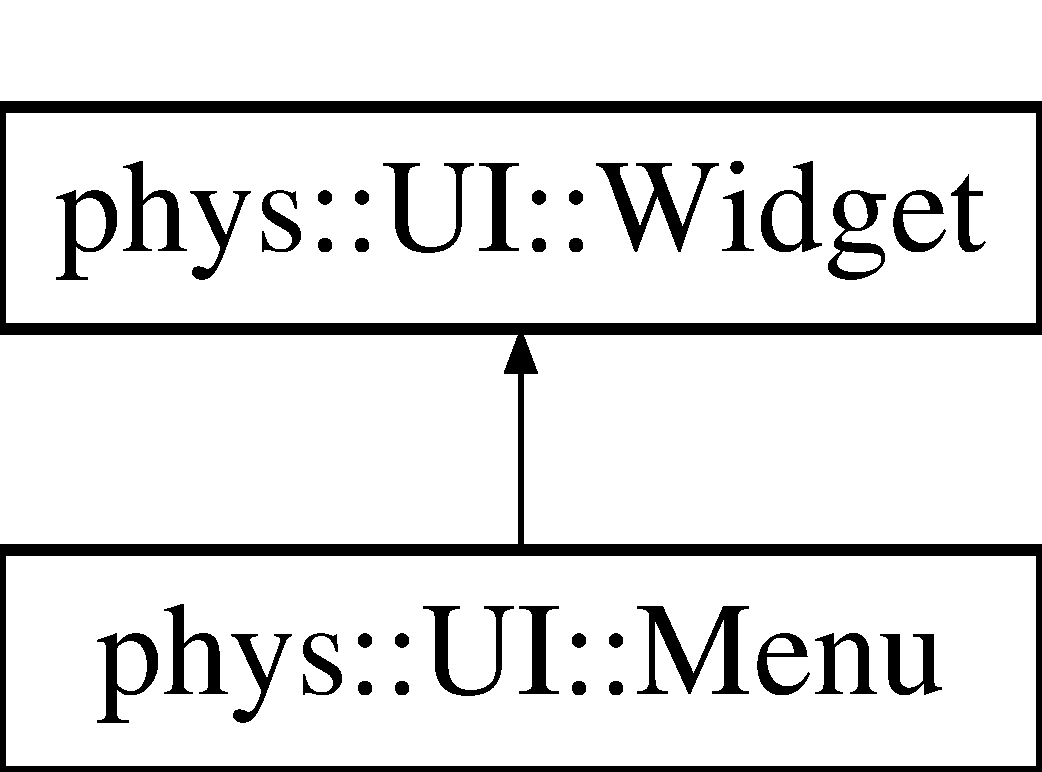
\includegraphics[height=2.000000cm]{classphys_1_1UI_1_1Menu}
\end{center}
\end{figure}
\subsubsection*{Public Member Functions}
\begin{DoxyCompactItemize}
\item 
virtual bool \hyperlink{classphys_1_1UI_1_1Menu_af2514d2614322856f604be2e167d0872}{CheckMouseHover} ()
\begin{DoxyCompactList}\small\item\em Checks to see if the current mouse position is over this menu. \item\end{DoxyCompactList}\item 
virtual \hyperlink{classphys_1_1Vector2}{Vector2} \hyperlink{classphys_1_1UI_1_1Menu_a74a1b8e9b1c5d36c12e5a0a7f813c40a}{GetActualPosition} ()
\begin{DoxyCompactList}\small\item\em Sets the pixel position of this menu. \item\end{DoxyCompactList}\item 
virtual \hyperlink{classphys_1_1Vector2}{Vector2} \hyperlink{classphys_1_1UI_1_1Menu_af7566b83c50a4a02ac78d174d7c61817}{GetActualSize} ()
\begin{DoxyCompactList}\small\item\em Sets the pixel size of this menu. \item\end{DoxyCompactList}\item 
virtual \hyperlink{classphys_1_1Vector2}{Vector2} \hyperlink{classphys_1_1UI_1_1Menu_a3c19fe2596fe4049325cc580daa70387}{GetPosition} ()
\begin{DoxyCompactList}\small\item\em Gets the relative position of this menu. \item\end{DoxyCompactList}\item 
virtual \hyperlink{classphys_1_1UI_1_1MenuWindow}{UI::MenuWindow} $\ast$ \hyperlink{classphys_1_1UI_1_1Menu_a9926f44b122c804b68034a759ea4a967}{GetRootWindow} ()
\begin{DoxyCompactList}\small\item\em Gets the Root window of this menu. \item\end{DoxyCompactList}\item 
virtual \hyperlink{classphys_1_1Vector2}{Vector2} \hyperlink{classphys_1_1UI_1_1Menu_a81781199a62bbe7c2e7693ef301223b4}{GetSize} ()
\begin{DoxyCompactList}\small\item\em Gets the relative size of this menu. \item\end{DoxyCompactList}\item 
virtual \hyperlink{classphys_1_1UI_1_1MenuWindow}{UI::MenuWindow} $\ast$ \hyperlink{classphys_1_1UI_1_1Menu_acf9a3bc3dd097093cce077cc60c14a6f}{GetTopWindow} ()
\begin{DoxyCompactList}\small\item\em Gets the current window at the top of the stack. \item\end{DoxyCompactList}\item 
\hypertarget{classphys_1_1UI_1_1Menu_a23f7b18c8bae528dc15bf8f3ff40d435}{
virtual void \hyperlink{classphys_1_1UI_1_1Menu_a23f7b18c8bae528dc15bf8f3ff40d435}{Hide} ()}
\label{classphys_1_1UI_1_1Menu_a23f7b18c8bae528dc15bf8f3ff40d435}

\begin{DoxyCompactList}\small\item\em Forces this menu to hide. \item\end{DoxyCompactList}\item 
\hyperlink{classphys_1_1UI_1_1Menu_abe99c5c7a18947dde5d3f44ce6fa0727}{Menu} (\hyperlink{namespacephys_a5ce5049f8b4bf88d6413c47b504ebb31}{ConstString} name, const \hyperlink{structphys_1_1UI_1_1RenderableRect}{RenderableRect} \&Rect, \hyperlink{classphys_1_1UI_1_1Layer}{Layer} $\ast$PLayer)
\begin{DoxyCompactList}\small\item\em Standard initialization constructor. \item\end{DoxyCompactList}\item 
virtual void \hyperlink{classphys_1_1UI_1_1Menu_a7eb3efc2675bf281a829f69416b46327}{RollMenuBackToWindow} (\hyperlink{classphys_1_1UI_1_1MenuWindow}{UI::MenuWindow} $\ast$Win)
\begin{DoxyCompactList}\small\item\em Hides and removes from the stack all windows from the top until it reaches the specified window, or root window. \item\end{DoxyCompactList}\item 
virtual void \hyperlink{classphys_1_1UI_1_1Menu_a1d5434382755df214b169d3e9901c1e1}{SetActualPosition} (const \hyperlink{classphys_1_1Vector2}{Vector2} \&Position)
\begin{DoxyCompactList}\small\item\em Sets the pixel position of this menu. \item\end{DoxyCompactList}\item 
virtual void \hyperlink{classphys_1_1UI_1_1Menu_acc3fb39539fd3c13def35be54570ae81}{SetActualSize} (const \hyperlink{classphys_1_1Vector2}{Vector2} \&Size)
\begin{DoxyCompactList}\small\item\em Sets the pixel size of this menu. \item\end{DoxyCompactList}\item 
virtual void \hyperlink{classphys_1_1UI_1_1Menu_a53ff13bb9b850fb8196c1c0c637afbd5}{SetPosition} (const \hyperlink{classphys_1_1Vector2}{Vector2} \&Position)
\begin{DoxyCompactList}\small\item\em Sets the relative position of this menu. \item\end{DoxyCompactList}\item 
virtual void \hyperlink{classphys_1_1UI_1_1Menu_adef3f9d3351c959f711e929a5e1c8f76}{SetSize} (const \hyperlink{classphys_1_1Vector2}{Vector2} \&Size)
\begin{DoxyCompactList}\small\item\em Sets the relative size of this menu. \item\end{DoxyCompactList}\item 
virtual void \hyperlink{classphys_1_1UI_1_1Menu_a4847e0de055a9c2f708f98742fa59a87}{SetVisible} (bool visible)
\begin{DoxyCompactList}\small\item\em Sets the visibility of this menu. \item\end{DoxyCompactList}\item 
\hypertarget{classphys_1_1UI_1_1Menu_aeb6373cc1be7da0bf5966129f271c861}{
virtual void \hyperlink{classphys_1_1UI_1_1Menu_aeb6373cc1be7da0bf5966129f271c861}{Show} ()}
\label{classphys_1_1UI_1_1Menu_aeb6373cc1be7da0bf5966129f271c861}

\begin{DoxyCompactList}\small\item\em Forces this menu to be shown. \item\end{DoxyCompactList}\item 
virtual void \hyperlink{classphys_1_1UI_1_1Menu_a60a678cc2be8f3eebfe65b3628557928}{UpdateDimensions} (const \hyperlink{classphys_1_1Vector2}{Vector2} \&NewViewportSize)
\begin{DoxyCompactList}\small\item\em Updates the dimensions of this widget to match those of the new screen size. \item\end{DoxyCompactList}\item 
\hypertarget{classphys_1_1UI_1_1Menu_a54b60c45238a3655da9dfa83104adb18}{
virtual \hyperlink{classphys_1_1UI_1_1Menu_a54b60c45238a3655da9dfa83104adb18}{$\sim$Menu} ()}
\label{classphys_1_1UI_1_1Menu_a54b60c45238a3655da9dfa83104adb18}

\begin{DoxyCompactList}\small\item\em Standard destructor. \item\end{DoxyCompactList}\end{DoxyCompactItemize}
\subsubsection*{Protected Member Functions}
\begin{DoxyCompactItemize}
\item 
\hypertarget{classphys_1_1UI_1_1Menu_a8759b8656fdbbc0e1231a3f8d2ad4835}{
virtual void \hyperlink{classphys_1_1UI_1_1Menu_a8759b8656fdbbc0e1231a3f8d2ad4835}{Update} (bool Force=false)}
\label{classphys_1_1UI_1_1Menu_a8759b8656fdbbc0e1231a3f8d2ad4835}

\begin{DoxyCompactList}\small\item\em For use with widget update/automation. \item\end{DoxyCompactList}\end{DoxyCompactItemize}
\subsubsection*{Protected Attributes}
\begin{DoxyCompactItemize}
\item 
\hypertarget{classphys_1_1UI_1_1Menu_a79081cb1d293f75fc69f20ed7e91dff6}{
std::vector$<$ \hyperlink{classphys_1_1UI_1_1MenuWindow}{UI::MenuWindow} $\ast$ $>$ {\bfseries MenuStack}}
\label{classphys_1_1UI_1_1Menu_a79081cb1d293f75fc69f20ed7e91dff6}

\item 
\hypertarget{classphys_1_1UI_1_1Menu_a02ca1c85ecb8cacf57c7fdad8ea16385}{
\hyperlink{classphys_1_1UI_1_1MenuWindow}{UI::MenuWindow} $\ast$ {\bfseries RootWindow}}
\label{classphys_1_1UI_1_1Menu_a02ca1c85ecb8cacf57c7fdad8ea16385}

\end{DoxyCompactItemize}


\subsubsection{Detailed Description}
This class is a control mechanism for multiple windows in a heirarchy. This class controls the presentation and order of different windows, useful for creating menu systems, be it a game main menu, or in-\/game menu. \par
 \par
 Also it should be noted that since this is just a control system for other classes, it doesn't have a position or size like other classes. Instead when you call those functions to set or get the position or size, you'll be working with the current top level window. 

Definition at line 62 of file uimenu.h.



\subsubsection{Constructor \& Destructor Documentation}
\hypertarget{classphys_1_1UI_1_1Menu_abe99c5c7a18947dde5d3f44ce6fa0727}{
\index{phys::UI::Menu@{phys::UI::Menu}!Menu@{Menu}}
\index{Menu@{Menu}!phys::UI::Menu@{phys::UI::Menu}}
\paragraph[{Menu}]{\setlength{\rightskip}{0pt plus 5cm}phys::UI::Menu::Menu (
\begin{DoxyParamCaption}
\item[{{\bf ConstString}}]{name, }
\item[{const {\bf RenderableRect} \&}]{Rect, }
\item[{{\bf Layer} $\ast$}]{PLayer}
\end{DoxyParamCaption}
)}\hfill}
\label{classphys_1_1UI_1_1Menu_abe99c5c7a18947dde5d3f44ce6fa0727}


Standard initialization constructor. 


\begin{DoxyParams}{Parameters}
{\em name} & The name of the window. \\
\hline
{\em Rect} & The Rect representing the position and size of the window. \\
\hline
{\em \hyperlink{classphys_1_1UI_1_1Layer}{Layer}} & The parent layer this window belongs to. \\
\hline
\end{DoxyParams}


Definition at line 57 of file uimenu.cpp.



\subsubsection{Member Function Documentation}
\hypertarget{classphys_1_1UI_1_1Menu_af2514d2614322856f604be2e167d0872}{
\index{phys::UI::Menu@{phys::UI::Menu}!CheckMouseHover@{CheckMouseHover}}
\index{CheckMouseHover@{CheckMouseHover}!phys::UI::Menu@{phys::UI::Menu}}
\paragraph[{CheckMouseHover}]{\setlength{\rightskip}{0pt plus 5cm}bool phys::UI::Menu::CheckMouseHover (
\begin{DoxyParamCaption}
{}
\end{DoxyParamCaption}
)\hspace{0.3cm}{\ttfamily  \mbox{[}virtual\mbox{]}}}\hfill}
\label{classphys_1_1UI_1_1Menu_af2514d2614322856f604be2e167d0872}


Checks to see if the current mouse position is over this menu. 

\begin{DoxyReturn}{Returns}
Returns a bool value, true if the mouse is over this menu, false if it's not. 
\end{DoxyReturn}


Implements \hyperlink{classphys_1_1UI_1_1Widget_a613df6dbb42efe139d185043a00259dc}{phys::UI::Widget}.



Definition at line 180 of file uimenu.cpp.

\hypertarget{classphys_1_1UI_1_1Menu_a74a1b8e9b1c5d36c12e5a0a7f813c40a}{
\index{phys::UI::Menu@{phys::UI::Menu}!GetActualPosition@{GetActualPosition}}
\index{GetActualPosition@{GetActualPosition}!phys::UI::Menu@{phys::UI::Menu}}
\paragraph[{GetActualPosition}]{\setlength{\rightskip}{0pt plus 5cm}{\bf Vector2} phys::UI::Menu::GetActualPosition (
\begin{DoxyParamCaption}
{}
\end{DoxyParamCaption}
)\hspace{0.3cm}{\ttfamily  \mbox{[}virtual\mbox{]}}}\hfill}
\label{classphys_1_1UI_1_1Menu_a74a1b8e9b1c5d36c12e5a0a7f813c40a}


Sets the pixel position of this menu. 

\begin{DoxyReturn}{Returns}
Returns a vector2 representing the pixel position of this menu. 
\end{DoxyReturn}


Implements \hyperlink{classphys_1_1UI_1_1Widget_a0a29fecff7f56d7909f65fd63b0990e7}{phys::UI::Widget}.



Definition at line 216 of file uimenu.cpp.

\hypertarget{classphys_1_1UI_1_1Menu_af7566b83c50a4a02ac78d174d7c61817}{
\index{phys::UI::Menu@{phys::UI::Menu}!GetActualSize@{GetActualSize}}
\index{GetActualSize@{GetActualSize}!phys::UI::Menu@{phys::UI::Menu}}
\paragraph[{GetActualSize}]{\setlength{\rightskip}{0pt plus 5cm}{\bf Vector2} phys::UI::Menu::GetActualSize (
\begin{DoxyParamCaption}
{}
\end{DoxyParamCaption}
)\hspace{0.3cm}{\ttfamily  \mbox{[}virtual\mbox{]}}}\hfill}
\label{classphys_1_1UI_1_1Menu_af7566b83c50a4a02ac78d174d7c61817}


Sets the pixel size of this menu. 

\begin{DoxyReturn}{Returns}
Returns a vector2 representing the pixel size of this menu. 
\end{DoxyReturn}


Implements \hyperlink{classphys_1_1UI_1_1Widget_af3a685621ed220748c0940ea38c96ed2}{phys::UI::Widget}.



Definition at line 236 of file uimenu.cpp.

\hypertarget{classphys_1_1UI_1_1Menu_a3c19fe2596fe4049325cc580daa70387}{
\index{phys::UI::Menu@{phys::UI::Menu}!GetPosition@{GetPosition}}
\index{GetPosition@{GetPosition}!phys::UI::Menu@{phys::UI::Menu}}
\paragraph[{GetPosition}]{\setlength{\rightskip}{0pt plus 5cm}{\bf Vector2} phys::UI::Menu::GetPosition (
\begin{DoxyParamCaption}
{}
\end{DoxyParamCaption}
)\hspace{0.3cm}{\ttfamily  \mbox{[}virtual\mbox{]}}}\hfill}
\label{classphys_1_1UI_1_1Menu_a3c19fe2596fe4049325cc580daa70387}


Gets the relative position of this menu. 

The position is relative to the screen size. Values range from 0.0 to 1.0. \begin{DoxyReturn}{Returns}
Returns a vector2 representing the relative position of this menu. 
\end{DoxyReturn}


Implements \hyperlink{classphys_1_1UI_1_1Widget_a3e464b028b0d1b5755923b8790260c33}{phys::UI::Widget}.



Definition at line 206 of file uimenu.cpp.

\hypertarget{classphys_1_1UI_1_1Menu_a9926f44b122c804b68034a759ea4a967}{
\index{phys::UI::Menu@{phys::UI::Menu}!GetRootWindow@{GetRootWindow}}
\index{GetRootWindow@{GetRootWindow}!phys::UI::Menu@{phys::UI::Menu}}
\paragraph[{GetRootWindow}]{\setlength{\rightskip}{0pt plus 5cm}{\bf MenuWindow} $\ast$ phys::UI::Menu::GetRootWindow (
\begin{DoxyParamCaption}
{}
\end{DoxyParamCaption}
)\hspace{0.3cm}{\ttfamily  \mbox{[}virtual\mbox{]}}}\hfill}
\label{classphys_1_1UI_1_1Menu_a9926f44b122c804b68034a759ea4a967}


Gets the Root window of this menu. 

\begin{DoxyReturn}{Returns}
Returns a pointer to the Root window of this menu. 
\end{DoxyReturn}


Definition at line 246 of file uimenu.cpp.

\hypertarget{classphys_1_1UI_1_1Menu_a81781199a62bbe7c2e7693ef301223b4}{
\index{phys::UI::Menu@{phys::UI::Menu}!GetSize@{GetSize}}
\index{GetSize@{GetSize}!phys::UI::Menu@{phys::UI::Menu}}
\paragraph[{GetSize}]{\setlength{\rightskip}{0pt plus 5cm}{\bf Vector2} phys::UI::Menu::GetSize (
\begin{DoxyParamCaption}
{}
\end{DoxyParamCaption}
)\hspace{0.3cm}{\ttfamily  \mbox{[}virtual\mbox{]}}}\hfill}
\label{classphys_1_1UI_1_1Menu_a81781199a62bbe7c2e7693ef301223b4}


Gets the relative size of this menu. 

The size is relative to the screen size. Values range from 0.0 to 1.0. \begin{DoxyReturn}{Returns}
Returns a vector2 representing the relative size of this menu. 
\end{DoxyReturn}


Implements \hyperlink{classphys_1_1UI_1_1Widget_a07039c19e57de314147ce066417da0a2}{phys::UI::Widget}.



Definition at line 226 of file uimenu.cpp.

\hypertarget{classphys_1_1UI_1_1Menu_acf9a3bc3dd097093cce077cc60c14a6f}{
\index{phys::UI::Menu@{phys::UI::Menu}!GetTopWindow@{GetTopWindow}}
\index{GetTopWindow@{GetTopWindow}!phys::UI::Menu@{phys::UI::Menu}}
\paragraph[{GetTopWindow}]{\setlength{\rightskip}{0pt plus 5cm}{\bf MenuWindow} $\ast$ phys::UI::Menu::GetTopWindow (
\begin{DoxyParamCaption}
{}
\end{DoxyParamCaption}
)\hspace{0.3cm}{\ttfamily  \mbox{[}virtual\mbox{]}}}\hfill}
\label{classphys_1_1UI_1_1Menu_acf9a3bc3dd097093cce077cc60c14a6f}


Gets the current window at the top of the stack. 

\begin{DoxyReturn}{Returns}
Returns a pointer to the window currently at the top of the stack. 
\end{DoxyReturn}


Definition at line 251 of file uimenu.cpp.

\hypertarget{classphys_1_1UI_1_1Menu_a7eb3efc2675bf281a829f69416b46327}{
\index{phys::UI::Menu@{phys::UI::Menu}!RollMenuBackToWindow@{RollMenuBackToWindow}}
\index{RollMenuBackToWindow@{RollMenuBackToWindow}!phys::UI::Menu@{phys::UI::Menu}}
\paragraph[{RollMenuBackToWindow}]{\setlength{\rightskip}{0pt plus 5cm}void phys::UI::Menu::RollMenuBackToWindow (
\begin{DoxyParamCaption}
\item[{{\bf UI::MenuWindow} $\ast$}]{Win}
\end{DoxyParamCaption}
)\hspace{0.3cm}{\ttfamily  \mbox{[}virtual\mbox{]}}}\hfill}
\label{classphys_1_1UI_1_1Menu_a7eb3efc2675bf281a829f69416b46327}


Hides and removes from the stack all windows from the top until it reaches the specified window, or root window. 


\begin{DoxyParams}{Parameters}
{\em Win} & The window to roll back to. \\
\hline
\end{DoxyParams}


Definition at line 128 of file uimenu.cpp.

\hypertarget{classphys_1_1UI_1_1Menu_a1d5434382755df214b169d3e9901c1e1}{
\index{phys::UI::Menu@{phys::UI::Menu}!SetActualPosition@{SetActualPosition}}
\index{SetActualPosition@{SetActualPosition}!phys::UI::Menu@{phys::UI::Menu}}
\paragraph[{SetActualPosition}]{\setlength{\rightskip}{0pt plus 5cm}void phys::UI::Menu::SetActualPosition (
\begin{DoxyParamCaption}
\item[{const {\bf Vector2} \&}]{Position}
\end{DoxyParamCaption}
)\hspace{0.3cm}{\ttfamily  \mbox{[}virtual\mbox{]}}}\hfill}
\label{classphys_1_1UI_1_1Menu_a1d5434382755df214b169d3e9901c1e1}


Sets the pixel position of this menu. 


\begin{DoxyParams}{Parameters}
{\em Position} & A vector2 representing the pixel position of this menu. \\
\hline
\end{DoxyParams}


Implements \hyperlink{classphys_1_1UI_1_1Widget_a77727351d98b10f1f4eb45048cb882e3}{phys::UI::Widget}.



Definition at line 211 of file uimenu.cpp.

\hypertarget{classphys_1_1UI_1_1Menu_acc3fb39539fd3c13def35be54570ae81}{
\index{phys::UI::Menu@{phys::UI::Menu}!SetActualSize@{SetActualSize}}
\index{SetActualSize@{SetActualSize}!phys::UI::Menu@{phys::UI::Menu}}
\paragraph[{SetActualSize}]{\setlength{\rightskip}{0pt plus 5cm}void phys::UI::Menu::SetActualSize (
\begin{DoxyParamCaption}
\item[{const {\bf Vector2} \&}]{Size}
\end{DoxyParamCaption}
)\hspace{0.3cm}{\ttfamily  \mbox{[}virtual\mbox{]}}}\hfill}
\label{classphys_1_1UI_1_1Menu_acc3fb39539fd3c13def35be54570ae81}


Sets the pixel size of this menu. 


\begin{DoxyParams}{Parameters}
{\em Size} & A vector2 representing the pixel size of this menu. \\
\hline
\end{DoxyParams}


Implements \hyperlink{classphys_1_1UI_1_1Widget_acda63a62fa158d5fe00c86f50e5c120d}{phys::UI::Widget}.



Definition at line 231 of file uimenu.cpp.

\hypertarget{classphys_1_1UI_1_1Menu_a53ff13bb9b850fb8196c1c0c637afbd5}{
\index{phys::UI::Menu@{phys::UI::Menu}!SetPosition@{SetPosition}}
\index{SetPosition@{SetPosition}!phys::UI::Menu@{phys::UI::Menu}}
\paragraph[{SetPosition}]{\setlength{\rightskip}{0pt plus 5cm}void phys::UI::Menu::SetPosition (
\begin{DoxyParamCaption}
\item[{const {\bf Vector2} \&}]{Position}
\end{DoxyParamCaption}
)\hspace{0.3cm}{\ttfamily  \mbox{[}virtual\mbox{]}}}\hfill}
\label{classphys_1_1UI_1_1Menu_a53ff13bb9b850fb8196c1c0c637afbd5}


Sets the relative position of this menu. 

The position is relative to the screen size. Values range from 0.0 to 1.0. 
\begin{DoxyParams}{Parameters}
{\em Position} & A vector2 representing the relative position of this menu. \\
\hline
\end{DoxyParams}


Implements \hyperlink{classphys_1_1UI_1_1Widget_a3ef894be2c0868105b2bf495ae944d00}{phys::UI::Widget}.



Definition at line 201 of file uimenu.cpp.

\hypertarget{classphys_1_1UI_1_1Menu_adef3f9d3351c959f711e929a5e1c8f76}{
\index{phys::UI::Menu@{phys::UI::Menu}!SetSize@{SetSize}}
\index{SetSize@{SetSize}!phys::UI::Menu@{phys::UI::Menu}}
\paragraph[{SetSize}]{\setlength{\rightskip}{0pt plus 5cm}void phys::UI::Menu::SetSize (
\begin{DoxyParamCaption}
\item[{const {\bf Vector2} \&}]{Size}
\end{DoxyParamCaption}
)\hspace{0.3cm}{\ttfamily  \mbox{[}virtual\mbox{]}}}\hfill}
\label{classphys_1_1UI_1_1Menu_adef3f9d3351c959f711e929a5e1c8f76}


Sets the relative size of this menu. 

The size is relative to the screen size. Values range from 0.0 to 1.0. 
\begin{DoxyParams}{Parameters}
{\em Size} & A vector2 representing the relative size of this menu. \\
\hline
\end{DoxyParams}


Implements \hyperlink{classphys_1_1UI_1_1Widget_a00f73c12583d25a75c089f944075b24d}{phys::UI::Widget}.



Definition at line 221 of file uimenu.cpp.

\hypertarget{classphys_1_1UI_1_1Menu_a4847e0de055a9c2f708f98742fa59a87}{
\index{phys::UI::Menu@{phys::UI::Menu}!SetVisible@{SetVisible}}
\index{SetVisible@{SetVisible}!phys::UI::Menu@{phys::UI::Menu}}
\paragraph[{SetVisible}]{\setlength{\rightskip}{0pt plus 5cm}void phys::UI::Menu::SetVisible (
\begin{DoxyParamCaption}
\item[{bool}]{visible}
\end{DoxyParamCaption}
)\hspace{0.3cm}{\ttfamily  \mbox{[}virtual\mbox{]}}}\hfill}
\label{classphys_1_1UI_1_1Menu_a4847e0de055a9c2f708f98742fa59a87}


Sets the visibility of this menu. 


\begin{DoxyParams}{Parameters}
{\em visible} & Bool determining whether or not this menu should be visible. \\
\hline
\end{DoxyParams}


Implements \hyperlink{classphys_1_1UI_1_1Widget_ab049233d8d5522a6ab42654b8924a3e0}{phys::UI::Widget}.



Definition at line 146 of file uimenu.cpp.

\hypertarget{classphys_1_1UI_1_1Menu_a60a678cc2be8f3eebfe65b3628557928}{
\index{phys::UI::Menu@{phys::UI::Menu}!UpdateDimensions@{UpdateDimensions}}
\index{UpdateDimensions@{UpdateDimensions}!phys::UI::Menu@{phys::UI::Menu}}
\paragraph[{UpdateDimensions}]{\setlength{\rightskip}{0pt plus 5cm}void phys::UI::Menu::UpdateDimensions (
\begin{DoxyParamCaption}
\item[{const {\bf Vector2} \&}]{NewViewportSize}
\end{DoxyParamCaption}
)\hspace{0.3cm}{\ttfamily  \mbox{[}virtual\mbox{]}}}\hfill}
\label{classphys_1_1UI_1_1Menu_a60a678cc2be8f3eebfe65b3628557928}


Updates the dimensions of this widget to match those of the new screen size. 

This function is called automatically when a viewport changes in size, and shouldn't need to be called manually. 
\begin{DoxyParams}{Parameters}
{\em NewViewportSize} & The new size of the viewport. \\
\hline
\end{DoxyParams}


Reimplemented from \hyperlink{classphys_1_1UI_1_1Widget_acbda7003549c6caac46078c034657929}{phys::UI::Widget}.



Definition at line 241 of file uimenu.cpp.



The documentation for this class was generated from the following files:\begin{DoxyCompactItemize}
\item 
uimenu.h\item 
uimenu.cpp\end{DoxyCompactItemize}

\hypertarget{classphys_1_1UI_1_1MenuWindow}{
\section{phys::UI::MenuWindow Class Reference}
\label{d4/d07/classphys_1_1UI_1_1MenuWindow}\index{phys::UI::MenuWindow@{phys::UI::MenuWindow}}
}


This class is an extended version of the window class for use exclusively with the menu widget.  




{\ttfamily \#include $<$uimenuwindow.h$>$}

Inheritance diagram for phys::UI::MenuWindow:\begin{figure}[H]
\begin{center}
\leavevmode
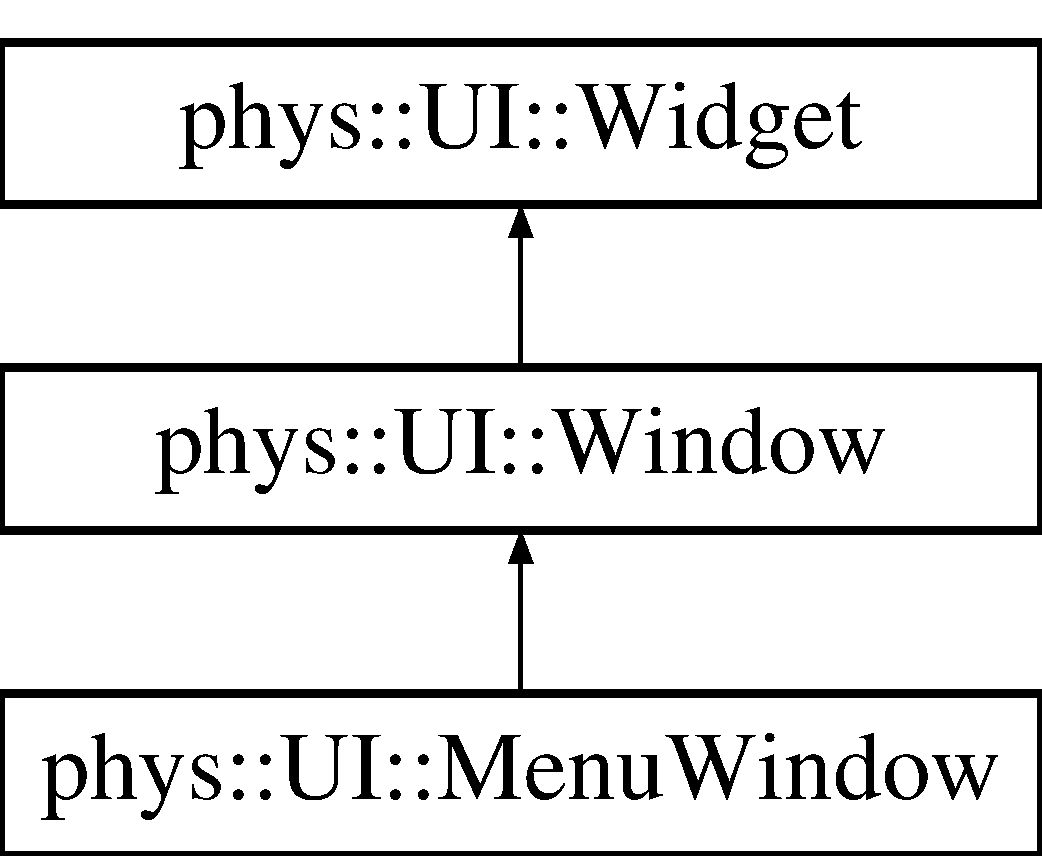
\includegraphics[height=3cm]{d4/d07/classphys_1_1UI_1_1MenuWindow}
\end{center}
\end{figure}
\subsection*{Public Member Functions}
\begin{DoxyCompactItemize}
\item 
\hyperlink{classphys_1_1UI_1_1MenuWindow_a8d62e0cdbb3e8073c62b67c3e0b4dfda}{MenuWindow} (\hyperlink{namespacephys_a5ce5049f8b4bf88d6413c47b504ebb31}{ConstString} \&Name, const \hyperlink{classphys_1_1Vector2}{Vector2} Position, const \hyperlink{classphys_1_1Vector2}{Vector2} Size, \hyperlink{classphys_1_1UI_1_1Menu}{UI::Menu} $\ast$TheMenu, \hyperlink{classphys_1_1UILayer}{UILayer} $\ast$Layer)
\begin{DoxyCompactList}\small\item\em Standard initialization constructor. \item\end{DoxyCompactList}\item 
\hypertarget{classphys_1_1UI_1_1MenuWindow_a8de1eab7a7897e24dfb722cce7d903eb}{
virtual \hyperlink{classphys_1_1UI_1_1MenuWindow_a8de1eab7a7897e24dfb722cce7d903eb}{$\sim$MenuWindow} ()}
\label{d4/d07/classphys_1_1UI_1_1MenuWindow_a8de1eab7a7897e24dfb722cce7d903eb}

\begin{DoxyCompactList}\small\item\em Standard destructor. \item\end{DoxyCompactList}\item 
virtual \hyperlink{classphys_1_1UI_1_1MenuWindow}{MenuWindow} $\ast$ \hyperlink{classphys_1_1UI_1_1MenuWindow_ac47ccc564f09ac33e13e56860b6ae281}{GetParentWindow} ()
\begin{DoxyCompactList}\small\item\em Gets the parent window of this window. \item\end{DoxyCompactList}\item 
virtual \hyperlink{classphys_1_1UI_1_1Button}{Button} $\ast$ \hyperlink{classphys_1_1UI_1_1MenuWindow_acb16433bca03c75b71ddb74d8df5b5ab}{CreateBackButton} (const \hyperlink{classphys_1_1Vector2}{Vector2} Position, const \hyperlink{classphys_1_1Vector2}{Vector2} Size)
\begin{DoxyCompactList}\small\item\em Creates a back button for this window. \item\end{DoxyCompactList}\item 
virtual \hyperlink{classphys_1_1UI_1_1Button}{Button} $\ast$ \hyperlink{classphys_1_1UI_1_1MenuWindow_a7c286758bac0e21154f41a56d9da8c08}{GetBackButton} ()
\begin{DoxyCompactList}\small\item\em Gets the back button of this window. \item\end{DoxyCompactList}\item 
virtual \hyperlink{classphys_1_1UI_1_1MenuWindow}{MenuWindow} $\ast$ \hyperlink{classphys_1_1UI_1_1MenuWindow_a12b1586cd33bc03b5902018376878961}{GetWindowOfAccessButton} (\hyperlink{classphys_1_1UI_1_1Button}{Button} $\ast$Accessor)
\begin{DoxyCompactList}\small\item\em Gets the \hyperlink{classphys_1_1UI_1_1Window}{Window} corresponding to the access button. \item\end{DoxyCompactList}\item 
virtual \hyperlink{classphys_1_1UI_1_1MenuWindow}{MenuWindow} $\ast$ \hyperlink{classphys_1_1UI_1_1MenuWindow_a5da3c65def5ce495685c086750e55132}{CreateChildMenuWindow} (\hyperlink{namespacephys_a5ce5049f8b4bf88d6413c47b504ebb31}{ConstString} \&Name, const \hyperlink{classphys_1_1Vector2}{Vector2} WinPosition, const \hyperlink{classphys_1_1Vector2}{Vector2} WinSize, const \hyperlink{classphys_1_1Vector2}{Vector2} ButPosition, const \hyperlink{classphys_1_1Vector2}{Vector2} ButSize)
\begin{DoxyCompactList}\small\item\em Adds a child window to this window. \item\end{DoxyCompactList}\item 
virtual \hyperlink{classphys_1_1UI_1_1MenuWindow}{MenuWindow} $\ast$ \hyperlink{classphys_1_1UI_1_1MenuWindow_ad1136c4e4b2ff9b9dc5d6aac2dba45a7}{GetChildMenuWindow} (\hyperlink{namespacephys_a5ce5049f8b4bf88d6413c47b504ebb31}{ConstString} \&Name)
\begin{DoxyCompactList}\small\item\em Gets an already created menu window by name. \item\end{DoxyCompactList}\item 
virtual \hyperlink{classphys_1_1UI_1_1MenuWindow}{MenuWindow} $\ast$ \hyperlink{classphys_1_1UI_1_1MenuWindow_a528d6397f8799219793978c70a26c22c}{GetChildMenuWindow} (const \hyperlink{namespacephys_a460f6bc24c8dd347b05e0366ae34f34a}{Whole} Index)
\begin{DoxyCompactList}\small\item\em Gets an already created menu window by index. \item\end{DoxyCompactList}\item 
virtual \hyperlink{namespacephys_a460f6bc24c8dd347b05e0366ae34f34a}{Whole} \hyperlink{classphys_1_1UI_1_1MenuWindow_ab3a6ae708ba2cea16cd0de176e265459}{GetNumChildMenuWindows} ()
\begin{DoxyCompactList}\small\item\em Gets the number of menu windows created and stored in this class. \item\end{DoxyCompactList}\item 
virtual void \hyperlink{classphys_1_1UI_1_1MenuWindow_ace2796c2d250fe1582f7c43333a7295e}{DestroyChildMenuWindow} (\hyperlink{classphys_1_1UI_1_1MenuWindow}{MenuWindow} $\ast$ToBeDestroyed)
\begin{DoxyCompactList}\small\item\em Destroys a menu window. \item\end{DoxyCompactList}\end{DoxyCompactItemize}
\subsection*{Protected Attributes}
\begin{DoxyCompactItemize}
\item 
\hypertarget{classphys_1_1UI_1_1MenuWindow_a94ec8861afbc6f39ac4b443a912bc0c1}{
\hyperlink{classphys_1_1UI_1_1MenuWindow}{MenuWindow} $\ast$ {\bfseries ParentWindow}}
\label{d4/d07/classphys_1_1UI_1_1MenuWindow_a94ec8861afbc6f39ac4b443a912bc0c1}

\item 
\hypertarget{classphys_1_1UI_1_1MenuWindow_adeed2fd68308846df8885febee141111}{
\hyperlink{classphys_1_1UI_1_1Menu}{UI::Menu} $\ast$ {\bfseries MasterMenu}}
\label{d4/d07/classphys_1_1UI_1_1MenuWindow_adeed2fd68308846df8885febee141111}

\item 
\hypertarget{classphys_1_1UI_1_1MenuWindow_a02826ad4a8d0b8934a7dbe86e4ea3edf}{
\hyperlink{classphys_1_1UI_1_1Button}{Button} $\ast$ {\bfseries BackButton}}
\label{d4/d07/classphys_1_1UI_1_1MenuWindow_a02826ad4a8d0b8934a7dbe86e4ea3edf}

\item 
\hypertarget{classphys_1_1UI_1_1MenuWindow_ae55c88520920e44c0bb125e812d62272}{
std::vector$<$ std::pair$<$ \hyperlink{classphys_1_1UI_1_1Button}{Button} $\ast$, \hyperlink{classphys_1_1UI_1_1MenuWindow}{MenuWindow} $\ast$ $>$ $>$ {\bfseries ChildWindows}}
\label{d4/d07/classphys_1_1UI_1_1MenuWindow_ae55c88520920e44c0bb125e812d62272}

\end{DoxyCompactItemize}


\subsection{Detailed Description}
This class is an extended version of the window class for use exclusively with the menu widget. 

Definition at line 60 of file uimenuwindow.h.



\subsection{Constructor \& Destructor Documentation}
\hypertarget{classphys_1_1UI_1_1MenuWindow_a8d62e0cdbb3e8073c62b67c3e0b4dfda}{
\index{phys::UI::MenuWindow@{phys::UI::MenuWindow}!MenuWindow@{MenuWindow}}
\index{MenuWindow@{MenuWindow}!phys::UI::MenuWindow@{phys::UI::MenuWindow}}
\subsubsection[{MenuWindow}]{\setlength{\rightskip}{0pt plus 5cm}phys::UI::MenuWindow::MenuWindow ({\bf ConstString} \& {\em Name}, \/  const {\bf Vector2} {\em Position}, \/  const {\bf Vector2} {\em Size}, \/  {\bf UI::Menu} $\ast$ {\em TheMenu}, \/  {\bf UILayer} $\ast$ {\em Layer})}}
\label{d4/d07/classphys_1_1UI_1_1MenuWindow_a8d62e0cdbb3e8073c62b67c3e0b4dfda}


Standard initialization constructor. 


\begin{DoxyParams}{Parameters}
\item[{\em Name}]The name of the window. \item[{\em Position}]The position of the window. \item[{\em Size}]The size of the window. \item[{\em TheMenu}]The menu this window belongs to. \item[{\em Layer}]The parent layer this window belongs to. \end{DoxyParams}


Definition at line 52 of file uimenuwindow.cpp.



\subsection{Member Function Documentation}
\hypertarget{classphys_1_1UI_1_1MenuWindow_acb16433bca03c75b71ddb74d8df5b5ab}{
\index{phys::UI::MenuWindow@{phys::UI::MenuWindow}!CreateBackButton@{CreateBackButton}}
\index{CreateBackButton@{CreateBackButton}!phys::UI::MenuWindow@{phys::UI::MenuWindow}}
\subsubsection[{CreateBackButton}]{\setlength{\rightskip}{0pt plus 5cm}{\bf Button} $\ast$ phys::UI::MenuWindow::CreateBackButton (const {\bf Vector2} {\em Position}, \/  const {\bf Vector2} {\em Size})\hspace{0.3cm}{\ttfamily  \mbox{[}virtual\mbox{]}}}}
\label{d4/d07/classphys_1_1UI_1_1MenuWindow_acb16433bca03c75b71ddb74d8df5b5ab}


Creates a back button for this window. 

The name is autogenerated to be the name of the window + \char`\"{}back\char`\"{}. This function will do nothing if the back button has already been created. \begin{DoxyReturn}{Returns}
Returns a pointer to the created Back \hyperlink{classphys_1_1UI_1_1Button}{Button}. 
\end{DoxyReturn}


Definition at line 75 of file uimenuwindow.cpp.

\hypertarget{classphys_1_1UI_1_1MenuWindow_a5da3c65def5ce495685c086750e55132}{
\index{phys::UI::MenuWindow@{phys::UI::MenuWindow}!CreateChildMenuWindow@{CreateChildMenuWindow}}
\index{CreateChildMenuWindow@{CreateChildMenuWindow}!phys::UI::MenuWindow@{phys::UI::MenuWindow}}
\subsubsection[{CreateChildMenuWindow}]{\setlength{\rightskip}{0pt plus 5cm}{\bf MenuWindow} $\ast$ phys::UI::MenuWindow::CreateChildMenuWindow ({\bf ConstString} \& {\em Name}, \/  const {\bf Vector2} {\em WinPosition}, \/  const {\bf Vector2} {\em WinSize}, \/  const {\bf Vector2} {\em ButPosition}, \/  const {\bf Vector2} {\em ButSize})\hspace{0.3cm}{\ttfamily  \mbox{[}virtual\mbox{]}}}}
\label{d4/d07/classphys_1_1UI_1_1MenuWindow_a5da3c65def5ce495685c086750e55132}


Adds a child window to this window. 

The name provided will become the windows name, the accompanying button will be the same +\char`\"{}button\char`\"{}. 
\begin{DoxyParams}{Parameters}
\item[{\em Name}]The name of the window. \item[{\em WinPosition}]The position of the window. \item[{\em WimSize}]The size of the window. \item[{\em ButPosition}]The position of the accompanying button. \item[{\em ButSize}]The size of the accompanying button. \end{DoxyParams}


Definition at line 106 of file uimenuwindow.cpp.

\hypertarget{classphys_1_1UI_1_1MenuWindow_ace2796c2d250fe1582f7c43333a7295e}{
\index{phys::UI::MenuWindow@{phys::UI::MenuWindow}!DestroyChildMenuWindow@{DestroyChildMenuWindow}}
\index{DestroyChildMenuWindow@{DestroyChildMenuWindow}!phys::UI::MenuWindow@{phys::UI::MenuWindow}}
\subsubsection[{DestroyChildMenuWindow}]{\setlength{\rightskip}{0pt plus 5cm}void phys::UI::MenuWindow::DestroyChildMenuWindow ({\bf MenuWindow} $\ast$ {\em ToBeDestroyed})\hspace{0.3cm}{\ttfamily  \mbox{[}virtual\mbox{]}}}}
\label{d4/d07/classphys_1_1UI_1_1MenuWindow_ace2796c2d250fe1582f7c43333a7295e}


Destroys a menu window. 


\begin{DoxyParams}{Parameters}
\item[{\em ToBeDestroyed}]Pointer to the menu window you want destroyed. \end{DoxyParams}


Definition at line 142 of file uimenuwindow.cpp.

\hypertarget{classphys_1_1UI_1_1MenuWindow_a7c286758bac0e21154f41a56d9da8c08}{
\index{phys::UI::MenuWindow@{phys::UI::MenuWindow}!GetBackButton@{GetBackButton}}
\index{GetBackButton@{GetBackButton}!phys::UI::MenuWindow@{phys::UI::MenuWindow}}
\subsubsection[{GetBackButton}]{\setlength{\rightskip}{0pt plus 5cm}{\bf Button} $\ast$ phys::UI::MenuWindow::GetBackButton ()\hspace{0.3cm}{\ttfamily  \mbox{[}virtual\mbox{]}}}}
\label{d4/d07/classphys_1_1UI_1_1MenuWindow_a7c286758bac0e21154f41a56d9da8c08}


Gets the back button of this window. 

\begin{DoxyReturn}{Returns}
Returns a pointer to the Back \hyperlink{classphys_1_1UI_1_1Button}{Button}, or NULL if it hasn't been created. 
\end{DoxyReturn}


Definition at line 88 of file uimenuwindow.cpp.

\hypertarget{classphys_1_1UI_1_1MenuWindow_a528d6397f8799219793978c70a26c22c}{
\index{phys::UI::MenuWindow@{phys::UI::MenuWindow}!GetChildMenuWindow@{GetChildMenuWindow}}
\index{GetChildMenuWindow@{GetChildMenuWindow}!phys::UI::MenuWindow@{phys::UI::MenuWindow}}
\subsubsection[{GetChildMenuWindow}]{\setlength{\rightskip}{0pt plus 5cm}{\bf MenuWindow} $\ast$ phys::UI::MenuWindow::GetChildMenuWindow (const {\bf Whole} {\em Index})\hspace{0.3cm}{\ttfamily  \mbox{[}virtual\mbox{]}}}}
\label{d4/d07/classphys_1_1UI_1_1MenuWindow_a528d6397f8799219793978c70a26c22c}


Gets an already created menu window by index. 

\begin{DoxyReturn}{Returns}
Returns a pointer to the menu window at the specified index. 
\end{DoxyReturn}


Definition at line 132 of file uimenuwindow.cpp.

\hypertarget{classphys_1_1UI_1_1MenuWindow_ad1136c4e4b2ff9b9dc5d6aac2dba45a7}{
\index{phys::UI::MenuWindow@{phys::UI::MenuWindow}!GetChildMenuWindow@{GetChildMenuWindow}}
\index{GetChildMenuWindow@{GetChildMenuWindow}!phys::UI::MenuWindow@{phys::UI::MenuWindow}}
\subsubsection[{GetChildMenuWindow}]{\setlength{\rightskip}{0pt plus 5cm}{\bf MenuWindow} $\ast$ phys::UI::MenuWindow::GetChildMenuWindow ({\bf ConstString} \& {\em Name})\hspace{0.3cm}{\ttfamily  \mbox{[}virtual\mbox{]}}}}
\label{d4/d07/classphys_1_1UI_1_1MenuWindow_ad1136c4e4b2ff9b9dc5d6aac2dba45a7}


Gets an already created menu window by name. 

\begin{DoxyReturn}{Returns}
Returns a pointer to the menu window of the specified name. 
\end{DoxyReturn}


Definition at line 119 of file uimenuwindow.cpp.

\hypertarget{classphys_1_1UI_1_1MenuWindow_ab3a6ae708ba2cea16cd0de176e265459}{
\index{phys::UI::MenuWindow@{phys::UI::MenuWindow}!GetNumChildMenuWindows@{GetNumChildMenuWindows}}
\index{GetNumChildMenuWindows@{GetNumChildMenuWindows}!phys::UI::MenuWindow@{phys::UI::MenuWindow}}
\subsubsection[{GetNumChildMenuWindows}]{\setlength{\rightskip}{0pt plus 5cm}{\bf Whole} phys::UI::MenuWindow::GetNumChildMenuWindows ()\hspace{0.3cm}{\ttfamily  \mbox{[}virtual\mbox{]}}}}
\label{d4/d07/classphys_1_1UI_1_1MenuWindow_ab3a6ae708ba2cea16cd0de176e265459}


Gets the number of menu windows created and stored in this class. 

\begin{DoxyReturn}{Returns}
Returns the number of menu windows this class is storing. 
\end{DoxyReturn}


Definition at line 137 of file uimenuwindow.cpp.

\hypertarget{classphys_1_1UI_1_1MenuWindow_ac47ccc564f09ac33e13e56860b6ae281}{
\index{phys::UI::MenuWindow@{phys::UI::MenuWindow}!GetParentWindow@{GetParentWindow}}
\index{GetParentWindow@{GetParentWindow}!phys::UI::MenuWindow@{phys::UI::MenuWindow}}
\subsubsection[{GetParentWindow}]{\setlength{\rightskip}{0pt plus 5cm}{\bf MenuWindow} $\ast$ phys::UI::MenuWindow::GetParentWindow ()\hspace{0.3cm}{\ttfamily  \mbox{[}virtual\mbox{]}}}}
\label{d4/d07/classphys_1_1UI_1_1MenuWindow_ac47ccc564f09ac33e13e56860b6ae281}


Gets the parent window of this window. 

\begin{DoxyReturn}{Returns}
Returns a pointer to the parent window of this window, or NULL if this is the root window. 
\end{DoxyReturn}


Definition at line 70 of file uimenuwindow.cpp.

\hypertarget{classphys_1_1UI_1_1MenuWindow_a12b1586cd33bc03b5902018376878961}{
\index{phys::UI::MenuWindow@{phys::UI::MenuWindow}!GetWindowOfAccessButton@{GetWindowOfAccessButton}}
\index{GetWindowOfAccessButton@{GetWindowOfAccessButton}!phys::UI::MenuWindow@{phys::UI::MenuWindow}}
\subsubsection[{GetWindowOfAccessButton}]{\setlength{\rightskip}{0pt plus 5cm}{\bf MenuWindow} $\ast$ phys::UI::MenuWindow::GetWindowOfAccessButton ({\bf Button} $\ast$ {\em Accessor})\hspace{0.3cm}{\ttfamily  \mbox{[}virtual\mbox{]}}}}
\label{d4/d07/classphys_1_1UI_1_1MenuWindow_a12b1586cd33bc03b5902018376878961}


Gets the \hyperlink{classphys_1_1UI_1_1Window}{Window} corresponding to the access button. 


\begin{DoxyParams}{Parameters}
\item[{\em Accessor}]Pointer to the \hyperlink{classphys_1_1UI_1_1Button}{Button} of which you want to get the window for. \end{DoxyParams}
\begin{DoxyReturn}{Returns}
Returns A pointer to the \hyperlink{classphys_1_1UI_1_1Menu}{Menu} window the button provided accesses. 
\end{DoxyReturn}


Definition at line 93 of file uimenuwindow.cpp.



The documentation for this class was generated from the following files:\begin{DoxyCompactItemize}
\item 
uimenuwindow.h\item 
uimenuwindow.cpp\end{DoxyCompactItemize}

\hypertarget{classphys_1_1MetaCode}{
\section{phys::MetaCode Class Reference}
\label{da/dc9/classphys_1_1MetaCode}\index{phys::MetaCode@{phys::MetaCode}}
}


This Determines the kind of user input.  




{\ttfamily \#include $<$metacode.h$>$}

\subsection*{Public Types}
\begin{DoxyCompactItemize}
\item 
enum \hyperlink{classphys_1_1MetaCode_a3e501cbb5bf0f6f1fdb7211465bda8d8}{InputCode} \{ \par
\hyperlink{classphys_1_1MetaCode_a3e501cbb5bf0f6f1fdb7211465bda8d8a061a36c9b5d9661314fd9d276b33042f}{KEY\_\-UNKNOWN} =  0, 
\hyperlink{classphys_1_1MetaCode_a3e501cbb5bf0f6f1fdb7211465bda8d8a45d7f3824a440f5bea5e616a6d6ea0b5}{KEY\_\-FIRST} =  0, 
{\bfseries KEY\_\-BACKSPACE} =  8, 
{\bfseries KEY\_\-TAB} =  9, 
\par
{\bfseries KEY\_\-CLEAR} =  12, 
{\bfseries KEY\_\-RETURN} =  13, 
{\bfseries KEY\_\-PAUSE} =  19, 
{\bfseries KEY\_\-ESCAPE} =  27, 
\par
{\bfseries KEY\_\-SPACE} =  32, 
{\bfseries KEY\_\-EXCLAIM} =  33, 
{\bfseries KEY\_\-QUOTEDBL} =  34, 
{\bfseries KEY\_\-HASH} =  35, 
\par
{\bfseries KEY\_\-DOLLAR} =  36, 
{\bfseries KEY\_\-AMPERSAND} =  38, 
{\bfseries KEY\_\-QUOTE} =  39, 
{\bfseries KEY\_\-LEFTPAREN} =  40, 
\par
{\bfseries KEY\_\-RIGHTPAREN} =  41, 
{\bfseries KEY\_\-ASTERISK} =  42, 
{\bfseries KEY\_\-PLUS} =  43, 
{\bfseries KEY\_\-COMMA} =  44, 
\par
{\bfseries KEY\_\-MINUS} =  45, 
{\bfseries KEY\_\-PERIOD} =  46, 
{\bfseries KEY\_\-SLASH} =  47, 
{\bfseries KEY\_\-0} =  48, 
\par
{\bfseries KEY\_\-1} =  49, 
{\bfseries KEY\_\-2} =  50, 
{\bfseries KEY\_\-3} =  51, 
{\bfseries KEY\_\-4} =  52, 
\par
{\bfseries KEY\_\-5} =  53, 
{\bfseries KEY\_\-6} =  54, 
{\bfseries KEY\_\-7} =  55, 
{\bfseries KEY\_\-8} =  56, 
\par
{\bfseries KEY\_\-9} =  57, 
{\bfseries KEY\_\-COLON} =  58, 
{\bfseries KEY\_\-SEMICOLON} =  59, 
{\bfseries KEY\_\-LESS} =  60, 
\par
{\bfseries KEY\_\-EQUALS} =  61, 
{\bfseries KEY\_\-GREATER} =  62, 
{\bfseries KEY\_\-QUESTION} =  63, 
{\bfseries KEY\_\-AT} =  64, 
\par
{\bfseries KEY\_\-LEFTBRACKET} =  91, 
{\bfseries KEY\_\-BACKSLASH} =  92, 
{\bfseries KEY\_\-RIGHTBRACKET} =  93, 
{\bfseries KEY\_\-CARET} =  94, 
\par
{\bfseries KEY\_\-UNDERSCORE} =  95, 
{\bfseries KEY\_\-BACKQUOTE} =  96, 
{\bfseries KEY\_\-a} =  97, 
{\bfseries KEY\_\-b} =  98, 
\par
{\bfseries KEY\_\-c} =  99, 
{\bfseries KEY\_\-d} =  100, 
{\bfseries KEY\_\-e} =  101, 
{\bfseries KEY\_\-f} =  102, 
\par
{\bfseries KEY\_\-g} =  103, 
{\bfseries KEY\_\-h} =  104, 
{\bfseries KEY\_\-i} =  105, 
{\bfseries KEY\_\-j} =  106, 
\par
{\bfseries KEY\_\-k} =  107, 
{\bfseries KEY\_\-l} =  108, 
{\bfseries KEY\_\-m} =  109, 
{\bfseries KEY\_\-n} =  110, 
\par
{\bfseries KEY\_\-o} =  111, 
{\bfseries KEY\_\-p} =  112, 
{\bfseries KEY\_\-q} =  113, 
{\bfseries KEY\_\-r} =  114, 
\par
{\bfseries KEY\_\-s} =  115, 
{\bfseries KEY\_\-t} =  116, 
{\bfseries KEY\_\-u} =  117, 
{\bfseries KEY\_\-v} =  118, 
\par
{\bfseries KEY\_\-w} =  119, 
{\bfseries KEY\_\-x} =  120, 
{\bfseries KEY\_\-y} =  121, 
{\bfseries KEY\_\-z} =  122, 
\par
{\bfseries KEY\_\-DELETE} =  127, 
{\bfseries KEY\_\-WORLD\_\-0} =  160, 
{\bfseries KEY\_\-WORLD\_\-1} =  161, 
{\bfseries KEY\_\-WORLD\_\-2} =  162, 
\par
{\bfseries KEY\_\-WORLD\_\-3} =  163, 
{\bfseries KEY\_\-WORLD\_\-4} =  164, 
{\bfseries KEY\_\-WORLD\_\-5} =  165, 
{\bfseries KEY\_\-WORLD\_\-6} =  166, 
\par
{\bfseries KEY\_\-WORLD\_\-7} =  167, 
{\bfseries KEY\_\-WORLD\_\-8} =  168, 
{\bfseries KEY\_\-WORLD\_\-9} =  169, 
{\bfseries KEY\_\-WORLD\_\-10} =  170, 
\par
{\bfseries KEY\_\-WORLD\_\-11} =  171, 
{\bfseries KEY\_\-WORLD\_\-12} =  172, 
{\bfseries KEY\_\-WORLD\_\-13} =  173, 
{\bfseries KEY\_\-WORLD\_\-14} =  174, 
\par
{\bfseries KEY\_\-WORLD\_\-15} =  175, 
{\bfseries KEY\_\-WORLD\_\-16} =  176, 
{\bfseries KEY\_\-WORLD\_\-17} =  177, 
{\bfseries KEY\_\-WORLD\_\-18} =  178, 
\par
{\bfseries KEY\_\-WORLD\_\-19} =  179, 
{\bfseries KEY\_\-WORLD\_\-20} =  180, 
{\bfseries KEY\_\-WORLD\_\-21} =  181, 
{\bfseries KEY\_\-WORLD\_\-22} =  182, 
\par
{\bfseries KEY\_\-WORLD\_\-23} =  183, 
{\bfseries KEY\_\-WORLD\_\-24} =  184, 
{\bfseries KEY\_\-WORLD\_\-25} =  185, 
{\bfseries KEY\_\-WORLD\_\-26} =  186, 
\par
{\bfseries KEY\_\-WORLD\_\-27} =  187, 
{\bfseries KEY\_\-WORLD\_\-28} =  188, 
{\bfseries KEY\_\-WORLD\_\-29} =  189, 
{\bfseries KEY\_\-WORLD\_\-30} =  190, 
\par
{\bfseries KEY\_\-WORLD\_\-31} =  191, 
{\bfseries KEY\_\-WORLD\_\-32} =  192, 
{\bfseries KEY\_\-WORLD\_\-33} =  193, 
{\bfseries KEY\_\-WORLD\_\-34} =  194, 
\par
{\bfseries KEY\_\-WORLD\_\-35} =  195, 
{\bfseries KEY\_\-WORLD\_\-36} =  196, 
{\bfseries KEY\_\-WORLD\_\-37} =  197, 
{\bfseries KEY\_\-WORLD\_\-38} =  198, 
\par
{\bfseries KEY\_\-WORLD\_\-39} =  199, 
{\bfseries KEY\_\-WORLD\_\-40} =  200, 
{\bfseries KEY\_\-WORLD\_\-41} =  201, 
{\bfseries KEY\_\-WORLD\_\-42} =  202, 
\par
{\bfseries KEY\_\-WORLD\_\-43} =  203, 
{\bfseries KEY\_\-WORLD\_\-44} =  204, 
{\bfseries KEY\_\-WORLD\_\-45} =  205, 
{\bfseries KEY\_\-WORLD\_\-46} =  206, 
\par
{\bfseries KEY\_\-WORLD\_\-47} =  207, 
{\bfseries KEY\_\-WORLD\_\-48} =  208, 
{\bfseries KEY\_\-WORLD\_\-49} =  209, 
{\bfseries KEY\_\-WORLD\_\-50} =  210, 
\par
{\bfseries KEY\_\-WORLD\_\-51} =  211, 
{\bfseries KEY\_\-WORLD\_\-52} =  212, 
{\bfseries KEY\_\-WORLD\_\-53} =  213, 
{\bfseries KEY\_\-WORLD\_\-54} =  214, 
\par
{\bfseries KEY\_\-WORLD\_\-55} =  215, 
{\bfseries KEY\_\-WORLD\_\-56} =  216, 
{\bfseries KEY\_\-WORLD\_\-57} =  217, 
{\bfseries KEY\_\-WORLD\_\-58} =  218, 
\par
{\bfseries KEY\_\-WORLD\_\-59} =  219, 
{\bfseries KEY\_\-WORLD\_\-60} =  220, 
{\bfseries KEY\_\-WORLD\_\-61} =  221, 
{\bfseries KEY\_\-WORLD\_\-62} =  222, 
\par
{\bfseries KEY\_\-WORLD\_\-63} =  223, 
{\bfseries KEY\_\-WORLD\_\-64} =  224, 
{\bfseries KEY\_\-WORLD\_\-65} =  225, 
{\bfseries KEY\_\-WORLD\_\-66} =  226, 
\par
{\bfseries KEY\_\-WORLD\_\-67} =  227, 
{\bfseries KEY\_\-WORLD\_\-68} =  228, 
{\bfseries KEY\_\-WORLD\_\-69} =  229, 
{\bfseries KEY\_\-WORLD\_\-70} =  230, 
\par
{\bfseries KEY\_\-WORLD\_\-71} =  231, 
{\bfseries KEY\_\-WORLD\_\-72} =  232, 
{\bfseries KEY\_\-WORLD\_\-73} =  233, 
{\bfseries KEY\_\-WORLD\_\-74} =  234, 
\par
{\bfseries KEY\_\-WORLD\_\-75} =  235, 
{\bfseries KEY\_\-WORLD\_\-76} =  236, 
{\bfseries KEY\_\-WORLD\_\-77} =  237, 
{\bfseries KEY\_\-WORLD\_\-78} =  238, 
\par
{\bfseries KEY\_\-WORLD\_\-79} =  239, 
{\bfseries KEY\_\-WORLD\_\-80} =  240, 
{\bfseries KEY\_\-WORLD\_\-81} =  241, 
{\bfseries KEY\_\-WORLD\_\-82} =  242, 
\par
{\bfseries KEY\_\-WORLD\_\-83} =  243, 
{\bfseries KEY\_\-WORLD\_\-84} =  244, 
{\bfseries KEY\_\-WORLD\_\-85} =  245, 
{\bfseries KEY\_\-WORLD\_\-86} =  246, 
\par
{\bfseries KEY\_\-WORLD\_\-87} =  247, 
{\bfseries KEY\_\-WORLD\_\-88} =  248, 
{\bfseries KEY\_\-WORLD\_\-89} =  249, 
{\bfseries KEY\_\-WORLD\_\-90} =  250, 
\par
{\bfseries KEY\_\-WORLD\_\-91} =  251, 
{\bfseries KEY\_\-WORLD\_\-92} =  252, 
{\bfseries KEY\_\-WORLD\_\-93} =  253, 
{\bfseries KEY\_\-WORLD\_\-94} =  254, 
\par
{\bfseries KEY\_\-WORLD\_\-95} =  255, 
{\bfseries KEY\_\-KP0} =  256, 
{\bfseries KEY\_\-KP1} =  257, 
{\bfseries KEY\_\-KP2} =  258, 
\par
{\bfseries KEY\_\-KP3} =  259, 
{\bfseries KEY\_\-KP4} =  260, 
{\bfseries KEY\_\-KP5} =  261, 
{\bfseries KEY\_\-KP6} =  262, 
\par
{\bfseries KEY\_\-KP7} =  263, 
{\bfseries KEY\_\-KP8} =  264, 
{\bfseries KEY\_\-KP9} =  265, 
{\bfseries KEY\_\-KP\_\-PERIOD} =  266, 
\par
{\bfseries KEY\_\-KP\_\-DIVIDE} =  267, 
{\bfseries KEY\_\-KP\_\-MULTIPLY} =  268, 
{\bfseries KEY\_\-KP\_\-MINUS} =  269, 
{\bfseries KEY\_\-KP\_\-PLUS} =  270, 
\par
{\bfseries KEY\_\-KP\_\-ENTER} =  271, 
{\bfseries KEY\_\-KP\_\-EQUALS} =  272, 
{\bfseries KEY\_\-UP} =  273, 
{\bfseries KEY\_\-DOWN} =  274, 
\par
{\bfseries KEY\_\-RIGHT} =  275, 
{\bfseries KEY\_\-LEFT} =  276, 
{\bfseries KEY\_\-INSERT} =  277, 
{\bfseries KEY\_\-HOME} =  278, 
\par
{\bfseries KEY\_\-END} =  279, 
{\bfseries KEY\_\-PAGEUP} =  280, 
{\bfseries KEY\_\-PAGEDOWN} =  281, 
{\bfseries KEY\_\-F1} =  282, 
\par
{\bfseries KEY\_\-F2} =  283, 
{\bfseries KEY\_\-F3} =  284, 
{\bfseries KEY\_\-F4} =  285, 
{\bfseries KEY\_\-F5} =  286, 
\par
{\bfseries KEY\_\-F6} =  287, 
{\bfseries KEY\_\-F7} =  288, 
{\bfseries KEY\_\-F8} =  289, 
{\bfseries KEY\_\-F9} =  290, 
\par
{\bfseries KEY\_\-F10} =  291, 
{\bfseries KEY\_\-F11} =  292, 
{\bfseries KEY\_\-F12} =  293, 
{\bfseries KEY\_\-F13} =  294, 
\par
{\bfseries KEY\_\-F14} =  295, 
{\bfseries KEY\_\-F15} =  296, 
{\bfseries KEY\_\-NUMLOCK} =  300, 
{\bfseries KEY\_\-CAPSLOCK} =  301, 
\par
{\bfseries KEY\_\-SCROLLOCK} =  302, 
{\bfseries KEY\_\-RSHIFT} =  303, 
{\bfseries KEY\_\-LSHIFT} =  304, 
{\bfseries KEY\_\-RCTRL} =  305, 
\par
{\bfseries KEY\_\-LCTRL} =  306, 
{\bfseries KEY\_\-RALT} =  307, 
{\bfseries KEY\_\-LALT} =  308, 
{\bfseries KEY\_\-RMETA} =  309, 
\par
{\bfseries KEY\_\-LMETA} =  310, 
\hyperlink{classphys_1_1MetaCode_a3e501cbb5bf0f6f1fdb7211465bda8d8aab77afaba4fc97faa9b9fe40d3a9ebbb}{KEY\_\-LSUPER} =  311, 
\hyperlink{classphys_1_1MetaCode_a3e501cbb5bf0f6f1fdb7211465bda8d8a84e2235ece031f83821867486ff52149}{KEY\_\-RSUPER} =  312, 
\hyperlink{classphys_1_1MetaCode_a3e501cbb5bf0f6f1fdb7211465bda8d8a9e26ea2006e876ccaa80fe4ae441da46}{KEY\_\-MODE} =  313, 
\par
\hyperlink{classphys_1_1MetaCode_a3e501cbb5bf0f6f1fdb7211465bda8d8aae92d5418d0273c8b43cb11f5e251a20}{KEY\_\-COMPOSE} =  314, 
{\bfseries KEY\_\-HELP} =  315, 
{\bfseries KEY\_\-PRINT} =  316, 
{\bfseries KEY\_\-SYSREQ} =  317, 
\par
{\bfseries KEY\_\-BREAK} =  318, 
{\bfseries KEY\_\-MENU} =  319, 
\hyperlink{classphys_1_1MetaCode_a3e501cbb5bf0f6f1fdb7211465bda8d8a08a2d04e3a40d746b81913e92a25a038}{KEY\_\-POWER} =  320, 
\hyperlink{classphys_1_1MetaCode_a3e501cbb5bf0f6f1fdb7211465bda8d8aee70075958d1650a7b48ba507103ec0c}{KEY\_\-EURO} =  321, 
\par
\hyperlink{classphys_1_1MetaCode_a3e501cbb5bf0f6f1fdb7211465bda8d8a15aabd8c4e36284ec057fafbda0d120a}{KEY\_\-UNDO} =  322, 
{\bfseries KEYMOD\_\-NONE} =  323, 
{\bfseries KEYMOD\_\-LSHIFT} =  324, 
{\bfseries KEYMOD\_\-RSHIFT} =  325, 
\par
{\bfseries KEYMOD\_\-LCTRL} =  326, 
{\bfseries KEYMOD\_\-RCTRL} =  327, 
{\bfseries KEYMOD\_\-LALT} =  328, 
{\bfseries KEYMOD\_\-RALT} =  329, 
\par
{\bfseries KEYMOD\_\-LMETA} =  330, 
{\bfseries KEYMOD\_\-RMETA} =  331, 
{\bfseries KEYMOD\_\-NUM} =  332, 
{\bfseries KEYMOD\_\-CAPS} =  333, 
\par
{\bfseries KEYMOD\_\-MODE} =  334, 
{\bfseries KEYMOD\_\-RESERVED} =  335, 
{\bfseries KEY\_\-LAST} =  379, 
\hyperlink{classphys_1_1MetaCode_a3e501cbb5bf0f6f1fdb7211465bda8d8a87685f9ca9462b329f2b86a17514f136}{INPUTEVENT\_\-FIRST} =  380, 
\par
\hyperlink{classphys_1_1MetaCode_a3e501cbb5bf0f6f1fdb7211465bda8d8a355649b334e903ada2496ad39dcd5f9d}{MOTION\_\-FIRST} =  460, 
\hyperlink{classphys_1_1MetaCode_a3e501cbb5bf0f6f1fdb7211465bda8d8a59cc92f5b2f42f7a138f8ea22e92d626}{MOTION\_\-LAST} =  469, 
\hyperlink{classphys_1_1MetaCode_a3e501cbb5bf0f6f1fdb7211465bda8d8acdb03d23d93022d5962db5026475b9c7}{MULTITOUCH\_\-FIRST} =  470, 
\hyperlink{classphys_1_1MetaCode_a3e501cbb5bf0f6f1fdb7211465bda8d8a94d804dc2330be620a8009252b5d5d22}{MULTITOUCH\_\-ACTION} =  471, 
\par
{\bfseries MULTITOUCH\_\-GESTURE} =  472, 
{\bfseries MULTITOUCH\_\-PINCH} =  473, 
{\bfseries MULTITOUCH\_\-STRETCH} =  474, 
{\bfseries MULTITOUCH\_\-LAST} =  479, 
\par
\hyperlink{classphys_1_1MetaCode_a3e501cbb5bf0f6f1fdb7211465bda8d8a1bb7f008c7d430e886141a3b8b697129}{MOUSE\_\-FIRST} =  480, 
\hyperlink{classphys_1_1MetaCode_a3e501cbb5bf0f6f1fdb7211465bda8d8a9cc80a2db206fb540fbb92a8ff64268a}{MOUSEBUTTON} =  481, 
{\bfseries MOUSEABSOLUTEVERTICAL} =  482, 
{\bfseries MOUSEABSOLUTEHORIZONTAL} =  483, 
\par
{\bfseries MOUSEVERTICAL} =  484, 
{\bfseries MOUSEHORIZONTAL} =  485, 
{\bfseries MOUSEWHEELVERTICAL} =  486, 
{\bfseries MOUSEWHEELHORIZONTAL} =  489, 
\par
{\bfseries MOUSE\_\-LAST} =  490, 
\hyperlink{classphys_1_1MetaCode_a3e501cbb5bf0f6f1fdb7211465bda8d8a666e564cae666de739b9b3cf047ec578}{JOYSTICK\_\-FIRST} =  499, 
\hyperlink{classphys_1_1MetaCode_a3e501cbb5bf0f6f1fdb7211465bda8d8aaaa2af6a60a9cd7403aa4786ef1ea389}{JOYSTICKBUTTON} =  500, 
{\bfseries JOYSTICKMOTIONAXIS} =  501, 
\par
{\bfseries JOYSTICKBALLVERTICAL} =  502, 
{\bfseries JOYSTICKBALLHORIZONTAL} =  503, 
{\bfseries JOYSTICKHATVERTICAL} =  504, 
{\bfseries JOYSTICKHATHORIZONTAL} =  505, 
\par
{\bfseries JOYSTICK\_\-LAST} =  506, 
\hyperlink{classphys_1_1MetaCode_a3e501cbb5bf0f6f1fdb7211465bda8d8adc78bfd04a85c4bbe39718f9acacbbe3}{INPUTEVENT\_\-LAST} =  512
 \}
\begin{DoxyCompactList}\small\item\em The InputCode enum defines all the posible types of inputs. \item\end{DoxyCompactList}\item 
enum \hyperlink{classphys_1_1MetaCode_a2fdfb26b3e50ceb0ccc60bfc4c3d6ac2}{ButtonState} \{ \hyperlink{classphys_1_1MetaCode_a2fdfb26b3e50ceb0ccc60bfc4c3d6ac2a6b5564408703517f36debd8c423e2dee}{BUTTON\_\-LIFTING} =  -\/1, 
\hyperlink{classphys_1_1MetaCode_a2fdfb26b3e50ceb0ccc60bfc4c3d6ac2ae275c52779b0f6ec37533af256a70cc3}{BUTTON\_\-UP} =  0, 
\hyperlink{classphys_1_1MetaCode_a2fdfb26b3e50ceb0ccc60bfc4c3d6ac2a33669b2b9ca814664296da55702e412d}{BUTTON\_\-PRESSING} =  1, 
\hyperlink{classphys_1_1MetaCode_a2fdfb26b3e50ceb0ccc60bfc4c3d6ac2a5b52ee1db94dbc2db23f3b4c267b5438}{BUTTON\_\-DOWN} =  2
 \}
\begin{DoxyCompactList}\small\item\em An Optional listing of value that can be used in a metacode to represent the information of a button press. \item\end{DoxyCompactList}\item 
enum \hyperlink{classphys_1_1MetaCode_af9ba277d1ef071be8861e35c2b7d82d6}{MouseWheelState} \{ \hyperlink{classphys_1_1MetaCode_af9ba277d1ef071be8861e35c2b7d82d6a15542262fc8fe9a3d6746f2b84ecde11}{MOUSEWHEEL\_\-UP} =  1, 
\hyperlink{classphys_1_1MetaCode_af9ba277d1ef071be8861e35c2b7d82d6aa3d86fe74d1c191d7c57f886c0b8d99a}{MOUSEWHEEL\_\-UNCHANGED} =  0, 
\hyperlink{classphys_1_1MetaCode_af9ba277d1ef071be8861e35c2b7d82d6ab6edd0886d2ec2d2917bbad96ce3d510}{MOUSEWHEEL\_\-DOWN} =  -\/1
 \}
\begin{DoxyCompactList}\small\item\em An Optional listing of values that can be used in a metacode Indicate spin of a mouse wheel. \item\end{DoxyCompactList}\end{DoxyCompactItemize}
\subsection*{Public Member Functions}
\begin{DoxyCompactItemize}
\item 
\hyperlink{classphys_1_1MetaCode_ae2c80c84f924ddfd880f46ffe6a1746e}{MetaCode} ()
\begin{DoxyCompactList}\small\item\em Default constructor. \item\end{DoxyCompactList}\item 
\hyperlink{classphys_1_1MetaCode_a05bcc50a09a9a5d19520dc258841f117}{MetaCode} (const int \&MetaValue\_\-, const short unsigned int \&ID\_\-, const \hyperlink{classphys_1_1MetaCode_a3e501cbb5bf0f6f1fdb7211465bda8d8}{MetaCode::InputCode} \&Code\_\-)
\begin{DoxyCompactList}\small\item\em Descriptive Constructor. \item\end{DoxyCompactList}\item 
\hyperlink{classphys_1_1MetaCode_ad9a618b5cc6f9d0cf0a4bc4f47bf98e8}{MetaCode} (const RawEvent \&RawEvent\_\-)
\begin{DoxyCompactList}\small\item\em The Heavy Lifting Constructor. \item\end{DoxyCompactList}\item 
\hyperlink{classphys_1_1MetaCode_a3e501cbb5bf0f6f1fdb7211465bda8d8}{MetaCode::InputCode} \hyperlink{classphys_1_1MetaCode_a5835a05391cbb5a3dc83534a7bcf87d3}{GetCode} () const 
\begin{DoxyCompactList}\small\item\em This Returns the Inputcode. \item\end{DoxyCompactList}\item 
void \hyperlink{classphys_1_1MetaCode_ab6759fbee9d039cf248bf76dde0f33dd}{SetCode} (const \hyperlink{classphys_1_1MetaCode_a3e501cbb5bf0f6f1fdb7211465bda8d8}{MetaCode::InputCode} \&Code\_\-)
\begin{DoxyCompactList}\small\item\em This Sets The InputCode. \item\end{DoxyCompactList}\item 
int \hyperlink{classphys_1_1MetaCode_ad8e7e4e7c6cdc6a05b8522910ce90cd4}{GetMetaValue} () const 
\begin{DoxyCompactList}\small\item\em This Returns the MetaValue. \item\end{DoxyCompactList}\item 
void \hyperlink{classphys_1_1MetaCode_a31a6390626b08c1bbf08e3f68d2ea764}{SetMetaValue} (const int \&MetaValue\_\-)
\begin{DoxyCompactList}\small\item\em This Sets The MetaValue. \item\end{DoxyCompactList}\item 
short unsigned int \hyperlink{classphys_1_1MetaCode_a70389ebd99493248fe93c598e2fe06c9}{GetID} () const 
\begin{DoxyCompactList}\small\item\em This Returns the Input ID. \item\end{DoxyCompactList}\item 
void \hyperlink{classphys_1_1MetaCode_a0ef70c11c06f0e3015121985cb1b6153}{SetID} (const short unsigned int \&ID\_\-)
\begin{DoxyCompactList}\small\item\em This Sets The input ID. \item\end{DoxyCompactList}\item 
bool \hyperlink{classphys_1_1MetaCode_a506486e5a6f08d50a5af42fa6d48a7f5}{operator==} (const \hyperlink{classphys_1_1MetaCode}{MetaCode} \&other) const 
\begin{DoxyCompactList}\small\item\em Compares two MetaCodes for equality. \item\end{DoxyCompactList}\end{DoxyCompactItemize}


\subsection{Detailed Description}
This Determines the kind of user input. A Metacode contains the data that is passed around with an input event. It stores one type of button press or analog representation (Mouse move, joystick tilt, wheel spin, etc...). If it is an analog representation it will also store how far or how it is pushed, pressed, rotated, or whatever. Several of these can be used in combination to represent button combinations, or complex input combination (like portions of fighter game moves). The first 127 character line up with Ascii, Currently upper lase are omitted for brevity. 

Definition at line 89 of file metacode.h.



\subsection{Member Enumeration Documentation}
\hypertarget{classphys_1_1MetaCode_a2fdfb26b3e50ceb0ccc60bfc4c3d6ac2}{
\index{phys::MetaCode@{phys::MetaCode}!ButtonState@{ButtonState}}
\index{ButtonState@{ButtonState}!phys::MetaCode@{phys::MetaCode}}
\subsubsection[{ButtonState}]{\setlength{\rightskip}{0pt plus 5cm}enum {\bf phys::MetaCode::ButtonState}}}
\label{da/dc9/classphys_1_1MetaCode_a2fdfb26b3e50ceb0ccc60bfc4c3d6ac2}


An Optional listing of value that can be used in a metacode to represent the information of a button press. 

This is optional set of values that can make working with buttons easier. The values the engine pass via the the event manager will all use these whereever appropriate. \begin{Desc}
\item[Enumerator: ]\par
\begin{description}
\index{BUTTON\_\-LIFTING@{BUTTON\_\-LIFTING}!phys::MetaCode@{phys::MetaCode}}\index{phys::MetaCode@{phys::MetaCode}!BUTTON\_\-LIFTING@{BUTTON\_\-LIFTING}}\item[{\em 
\hypertarget{classphys_1_1MetaCode_a2fdfb26b3e50ceb0ccc60bfc4c3d6ac2a6b5564408703517f36debd8c423e2dee}{
BUTTON\_\-LIFTING}
\label{da/dc9/classphys_1_1MetaCode_a2fdfb26b3e50ceb0ccc60bfc4c3d6ac2a6b5564408703517f36debd8c423e2dee}
}]Used when the key stops being pressed. \index{BUTTON\_\-UP@{BUTTON\_\-UP}!phys::MetaCode@{phys::MetaCode}}\index{phys::MetaCode@{phys::MetaCode}!BUTTON\_\-UP@{BUTTON\_\-UP}}\item[{\em 
\hypertarget{classphys_1_1MetaCode_a2fdfb26b3e50ceb0ccc60bfc4c3d6ac2ae275c52779b0f6ec37533af256a70cc3}{
BUTTON\_\-UP}
\label{da/dc9/classphys_1_1MetaCode_a2fdfb26b3e50ceb0ccc60bfc4c3d6ac2ae275c52779b0f6ec37533af256a70cc3}
}]The default state of a key. \index{BUTTON\_\-PRESSING@{BUTTON\_\-PRESSING}!phys::MetaCode@{phys::MetaCode}}\index{phys::MetaCode@{phys::MetaCode}!BUTTON\_\-PRESSING@{BUTTON\_\-PRESSING}}\item[{\em 
\hypertarget{classphys_1_1MetaCode_a2fdfb26b3e50ceb0ccc60bfc4c3d6ac2a33669b2b9ca814664296da55702e412d}{
BUTTON\_\-PRESSING}
\label{da/dc9/classphys_1_1MetaCode_a2fdfb26b3e50ceb0ccc60bfc4c3d6ac2a33669b2b9ca814664296da55702e412d}
}]This is used at the exact point in time that a key goes from unpressed to pressed. \index{BUTTON\_\-DOWN@{BUTTON\_\-DOWN}!phys::MetaCode@{phys::MetaCode}}\index{phys::MetaCode@{phys::MetaCode}!BUTTON\_\-DOWN@{BUTTON\_\-DOWN}}\item[{\em 
\hypertarget{classphys_1_1MetaCode_a2fdfb26b3e50ceb0ccc60bfc4c3d6ac2a5b52ee1db94dbc2db23f3b4c267b5438}{
BUTTON\_\-DOWN}
\label{da/dc9/classphys_1_1MetaCode_a2fdfb26b3e50ceb0ccc60bfc4c3d6ac2a5b52ee1db94dbc2db23f3b4c267b5438}
}]This is used the entire time a key is down. \end{description}
\end{Desc}



Definition at line 400 of file metacode.h.

\hypertarget{classphys_1_1MetaCode_a3e501cbb5bf0f6f1fdb7211465bda8d8}{
\index{phys::MetaCode@{phys::MetaCode}!InputCode@{InputCode}}
\index{InputCode@{InputCode}!phys::MetaCode@{phys::MetaCode}}
\subsubsection[{InputCode}]{\setlength{\rightskip}{0pt plus 5cm}enum {\bf phys::MetaCode::InputCode}}}
\label{da/dc9/classphys_1_1MetaCode_a3e501cbb5bf0f6f1fdb7211465bda8d8}


The InputCode enum defines all the posible types of inputs. 

It has one entry for each key on a most keyboards. Then it has an entry for most mouse and joystick input methods. \begin{Desc}
\item[Enumerator: ]\par
\begin{description}
\index{KEY\_\-UNKNOWN@{KEY\_\-UNKNOWN}!phys::MetaCode@{phys::MetaCode}}\index{phys::MetaCode@{phys::MetaCode}!KEY\_\-UNKNOWN@{KEY\_\-UNKNOWN}}\item[{\em 
\hypertarget{classphys_1_1MetaCode_a3e501cbb5bf0f6f1fdb7211465bda8d8a061a36c9b5d9661314fd9d276b33042f}{
KEY\_\-UNKNOWN}
\label{da/dc9/classphys_1_1MetaCode_a3e501cbb5bf0f6f1fdb7211465bda8d8a061a36c9b5d9661314fd9d276b33042f}
}]KEY\_\-UNKNOWN This is used for unsupported keys or keys that are not in Unicode. \index{KEY\_\-FIRST@{KEY\_\-FIRST}!phys::MetaCode@{phys::MetaCode}}\index{phys::MetaCode@{phys::MetaCode}!KEY\_\-FIRST@{KEY\_\-FIRST}}\item[{\em 
\hypertarget{classphys_1_1MetaCode_a3e501cbb5bf0f6f1fdb7211465bda8d8a45d7f3824a440f5bea5e616a6d6ea0b5}{
KEY\_\-FIRST}
\label{da/dc9/classphys_1_1MetaCode_a3e501cbb5bf0f6f1fdb7211465bda8d8a45d7f3824a440f5bea5e616a6d6ea0b5}
}]KEY\_\-FIRST Same Value as KEY\_\-UNKOWN, is Guaranteed to be the lowest value of any key. \index{KEY\_\-LSUPER@{KEY\_\-LSUPER}!phys::MetaCode@{phys::MetaCode}}\index{phys::MetaCode@{phys::MetaCode}!KEY\_\-LSUPER@{KEY\_\-LSUPER}}\item[{\em 
\hypertarget{classphys_1_1MetaCode_a3e501cbb5bf0f6f1fdb7211465bda8d8aab77afaba4fc97faa9b9fe40d3a9ebbb}{
KEY\_\-LSUPER}
\label{da/dc9/classphys_1_1MetaCode_a3e501cbb5bf0f6f1fdb7211465bda8d8aab77afaba4fc97faa9b9fe40d3a9ebbb}
}]Left \char`\"{}Windows\char`\"{} key \index{KEY\_\-RSUPER@{KEY\_\-RSUPER}!phys::MetaCode@{phys::MetaCode}}\index{phys::MetaCode@{phys::MetaCode}!KEY\_\-RSUPER@{KEY\_\-RSUPER}}\item[{\em 
\hypertarget{classphys_1_1MetaCode_a3e501cbb5bf0f6f1fdb7211465bda8d8a84e2235ece031f83821867486ff52149}{
KEY\_\-RSUPER}
\label{da/dc9/classphys_1_1MetaCode_a3e501cbb5bf0f6f1fdb7211465bda8d8a84e2235ece031f83821867486ff52149}
}]Right \char`\"{}Windows\char`\"{} key \index{KEY\_\-MODE@{KEY\_\-MODE}!phys::MetaCode@{phys::MetaCode}}\index{phys::MetaCode@{phys::MetaCode}!KEY\_\-MODE@{KEY\_\-MODE}}\item[{\em 
\hypertarget{classphys_1_1MetaCode_a3e501cbb5bf0f6f1fdb7211465bda8d8a9e26ea2006e876ccaa80fe4ae441da46}{
KEY\_\-MODE}
\label{da/dc9/classphys_1_1MetaCode_a3e501cbb5bf0f6f1fdb7211465bda8d8a9e26ea2006e876ccaa80fe4ae441da46}
}]\char`\"{}Alt Gr\char`\"{} key \index{KEY\_\-COMPOSE@{KEY\_\-COMPOSE}!phys::MetaCode@{phys::MetaCode}}\index{phys::MetaCode@{phys::MetaCode}!KEY\_\-COMPOSE@{KEY\_\-COMPOSE}}\item[{\em 
\hypertarget{classphys_1_1MetaCode_a3e501cbb5bf0f6f1fdb7211465bda8d8aae92d5418d0273c8b43cb11f5e251a20}{
KEY\_\-COMPOSE}
\label{da/dc9/classphys_1_1MetaCode_a3e501cbb5bf0f6f1fdb7211465bda8d8aae92d5418d0273c8b43cb11f5e251a20}
}]Multi-\/key compose key \index{KEY\_\-POWER@{KEY\_\-POWER}!phys::MetaCode@{phys::MetaCode}}\index{phys::MetaCode@{phys::MetaCode}!KEY\_\-POWER@{KEY\_\-POWER}}\item[{\em 
\hypertarget{classphys_1_1MetaCode_a3e501cbb5bf0f6f1fdb7211465bda8d8a08a2d04e3a40d746b81913e92a25a038}{
KEY\_\-POWER}
\label{da/dc9/classphys_1_1MetaCode_a3e501cbb5bf0f6f1fdb7211465bda8d8a08a2d04e3a40d746b81913e92a25a038}
}]Power Macintosh power key \index{KEY\_\-EURO@{KEY\_\-EURO}!phys::MetaCode@{phys::MetaCode}}\index{phys::MetaCode@{phys::MetaCode}!KEY\_\-EURO@{KEY\_\-EURO}}\item[{\em 
\hypertarget{classphys_1_1MetaCode_a3e501cbb5bf0f6f1fdb7211465bda8d8aee70075958d1650a7b48ba507103ec0c}{
KEY\_\-EURO}
\label{da/dc9/classphys_1_1MetaCode_a3e501cbb5bf0f6f1fdb7211465bda8d8aee70075958d1650a7b48ba507103ec0c}
}]Some European keyboards \index{KEY\_\-UNDO@{KEY\_\-UNDO}!phys::MetaCode@{phys::MetaCode}}\index{phys::MetaCode@{phys::MetaCode}!KEY\_\-UNDO@{KEY\_\-UNDO}}\item[{\em 
\hypertarget{classphys_1_1MetaCode_a3e501cbb5bf0f6f1fdb7211465bda8d8a15aabd8c4e36284ec057fafbda0d120a}{
KEY\_\-UNDO}
\label{da/dc9/classphys_1_1MetaCode_a3e501cbb5bf0f6f1fdb7211465bda8d8a15aabd8c4e36284ec057fafbda0d120a}
}]Atari keyboard has Undo \index{INPUTEVENT\_\-FIRST@{INPUTEVENT\_\-FIRST}!phys::MetaCode@{phys::MetaCode}}\index{phys::MetaCode@{phys::MetaCode}!INPUTEVENT\_\-FIRST@{INPUTEVENT\_\-FIRST}}\item[{\em 
\hypertarget{classphys_1_1MetaCode_a3e501cbb5bf0f6f1fdb7211465bda8d8a87685f9ca9462b329f2b86a17514f136}{
INPUTEVENT\_\-FIRST}
\label{da/dc9/classphys_1_1MetaCode_a3e501cbb5bf0f6f1fdb7211465bda8d8a87685f9ca9462b329f2b86a17514f136}
}]The last KeyCode, all Keys values will be less than this, and all Events will be larger than that. \index{MOTION\_\-FIRST@{MOTION\_\-FIRST}!phys::MetaCode@{phys::MetaCode}}\index{phys::MetaCode@{phys::MetaCode}!MOTION\_\-FIRST@{MOTION\_\-FIRST}}\item[{\em 
\hypertarget{classphys_1_1MetaCode_a3e501cbb5bf0f6f1fdb7211465bda8d8a355649b334e903ada2496ad39dcd5f9d}{
MOTION\_\-FIRST}
\label{da/dc9/classphys_1_1MetaCode_a3e501cbb5bf0f6f1fdb7211465bda8d8a355649b334e903ada2496ad39dcd5f9d}
}]The First non-\/event, all Keys values will be Less than this. \index{MOTION\_\-LAST@{MOTION\_\-LAST}!phys::MetaCode@{phys::MetaCode}}\index{phys::MetaCode@{phys::MetaCode}!MOTION\_\-LAST@{MOTION\_\-LAST}}\item[{\em 
\hypertarget{classphys_1_1MetaCode_a3e501cbb5bf0f6f1fdb7211465bda8d8a59cc92f5b2f42f7a138f8ea22e92d626}{
MOTION\_\-LAST}
\label{da/dc9/classphys_1_1MetaCode_a3e501cbb5bf0f6f1fdb7211465bda8d8a59cc92f5b2f42f7a138f8ea22e92d626}
}]The first Motion event. \index{MULTITOUCH\_\-FIRST@{MULTITOUCH\_\-FIRST}!phys::MetaCode@{phys::MetaCode}}\index{phys::MetaCode@{phys::MetaCode}!MULTITOUCH\_\-FIRST@{MULTITOUCH\_\-FIRST}}\item[{\em 
\hypertarget{classphys_1_1MetaCode_a3e501cbb5bf0f6f1fdb7211465bda8d8acdb03d23d93022d5962db5026475b9c7}{
MULTITOUCH\_\-FIRST}
\label{da/dc9/classphys_1_1MetaCode_a3e501cbb5bf0f6f1fdb7211465bda8d8acdb03d23d93022d5962db5026475b9c7}
}]The last Motion event. \index{MULTITOUCH\_\-ACTION@{MULTITOUCH\_\-ACTION}!phys::MetaCode@{phys::MetaCode}}\index{phys::MetaCode@{phys::MetaCode}!MULTITOUCH\_\-ACTION@{MULTITOUCH\_\-ACTION}}\item[{\em 
\hypertarget{classphys_1_1MetaCode_a3e501cbb5bf0f6f1fdb7211465bda8d8a94d804dc2330be620a8009252b5d5d22}{
MULTITOUCH\_\-ACTION}
\label{da/dc9/classphys_1_1MetaCode_a3e501cbb5bf0f6f1fdb7211465bda8d8a94d804dc2330be620a8009252b5d5d22}
}]The first Multi Touch event. \index{MOUSE\_\-FIRST@{MOUSE\_\-FIRST}!phys::MetaCode@{phys::MetaCode}}\index{phys::MetaCode@{phys::MetaCode}!MOUSE\_\-FIRST@{MOUSE\_\-FIRST}}\item[{\em 
\hypertarget{classphys_1_1MetaCode_a3e501cbb5bf0f6f1fdb7211465bda8d8a1bb7f008c7d430e886141a3b8b697129}{
MOUSE\_\-FIRST}
\label{da/dc9/classphys_1_1MetaCode_a3e501cbb5bf0f6f1fdb7211465bda8d8a1bb7f008c7d430e886141a3b8b697129}
}]The last Multi Touch event. \index{MOUSEBUTTON@{MOUSEBUTTON}!phys::MetaCode@{phys::MetaCode}}\index{phys::MetaCode@{phys::MetaCode}!MOUSEBUTTON@{MOUSEBUTTON}}\item[{\em 
\hypertarget{classphys_1_1MetaCode_a3e501cbb5bf0f6f1fdb7211465bda8d8a9cc80a2db206fb540fbb92a8ff64268a}{
MOUSEBUTTON}
\label{da/dc9/classphys_1_1MetaCode_a3e501cbb5bf0f6f1fdb7211465bda8d8a9cc80a2db206fb540fbb92a8ff64268a}
}]The First Mouse event, all Mouse \hyperlink{classphys_1_1Event}{Event} values will be more than this. \index{JOYSTICK\_\-FIRST@{JOYSTICK\_\-FIRST}!phys::MetaCode@{phys::MetaCode}}\index{phys::MetaCode@{phys::MetaCode}!JOYSTICK\_\-FIRST@{JOYSTICK\_\-FIRST}}\item[{\em 
\hypertarget{classphys_1_1MetaCode_a3e501cbb5bf0f6f1fdb7211465bda8d8a666e564cae666de739b9b3cf047ec578}{
JOYSTICK\_\-FIRST}
\label{da/dc9/classphys_1_1MetaCode_a3e501cbb5bf0f6f1fdb7211465bda8d8a666e564cae666de739b9b3cf047ec578}
}]The last MouseEvent Code, all Mouse events will be less than this. \index{JOYSTICKBUTTON@{JOYSTICKBUTTON}!phys::MetaCode@{phys::MetaCode}}\index{phys::MetaCode@{phys::MetaCode}!JOYSTICKBUTTON@{JOYSTICKBUTTON}}\item[{\em 
\hypertarget{classphys_1_1MetaCode_a3e501cbb5bf0f6f1fdb7211465bda8d8aaaa2af6a60a9cd7403aa4786ef1ea389}{
JOYSTICKBUTTON}
\label{da/dc9/classphys_1_1MetaCode_a3e501cbb5bf0f6f1fdb7211465bda8d8aaaa2af6a60a9cd7403aa4786ef1ea389}
}]The First JoyStick event, all Joystick \hyperlink{classphys_1_1Event}{Event} values will be more than this. \index{INPUTEVENT\_\-LAST@{INPUTEVENT\_\-LAST}!phys::MetaCode@{phys::MetaCode}}\index{phys::MetaCode@{phys::MetaCode}!INPUTEVENT\_\-LAST@{INPUTEVENT\_\-LAST}}\item[{\em 
\hypertarget{classphys_1_1MetaCode_a3e501cbb5bf0f6f1fdb7211465bda8d8adc78bfd04a85c4bbe39718f9acacbbe3}{
INPUTEVENT\_\-LAST}
\label{da/dc9/classphys_1_1MetaCode_a3e501cbb5bf0f6f1fdb7211465bda8d8adc78bfd04a85c4bbe39718f9acacbbe3}
}]The last JoyStick \hyperlink{classphys_1_1Event}{Event} Code, all JoyStick events will be less than this. \end{description}
\end{Desc}



Definition at line 96 of file metacode.h.

\hypertarget{classphys_1_1MetaCode_af9ba277d1ef071be8861e35c2b7d82d6}{
\index{phys::MetaCode@{phys::MetaCode}!MouseWheelState@{MouseWheelState}}
\index{MouseWheelState@{MouseWheelState}!phys::MetaCode@{phys::MetaCode}}
\subsubsection[{MouseWheelState}]{\setlength{\rightskip}{0pt plus 5cm}enum {\bf phys::MetaCode::MouseWheelState}}}
\label{da/dc9/classphys_1_1MetaCode_af9ba277d1ef071be8861e35c2b7d82d6}


An Optional listing of values that can be used in a metacode Indicate spin of a mouse wheel. 

This is optional set of values that can make working with the MouseWheel easier. The values the engine pass via the the event manager will all use these whereever appropriate. \begin{Desc}
\item[Enumerator: ]\par
\begin{description}
\index{MOUSEWHEEL\_\-UP@{MOUSEWHEEL\_\-UP}!phys::MetaCode@{phys::MetaCode}}\index{phys::MetaCode@{phys::MetaCode}!MOUSEWHEEL\_\-UP@{MOUSEWHEEL\_\-UP}}\item[{\em 
\hypertarget{classphys_1_1MetaCode_af9ba277d1ef071be8861e35c2b7d82d6a15542262fc8fe9a3d6746f2b84ecde11}{
MOUSEWHEEL\_\-UP}
\label{da/dc9/classphys_1_1MetaCode_af9ba277d1ef071be8861e35c2b7d82d6a15542262fc8fe9a3d6746f2b84ecde11}
}]Optionally Used when the MouseWheel is spun up as a Meta Code \index{MOUSEWHEEL\_\-UNCHANGED@{MOUSEWHEEL\_\-UNCHANGED}!phys::MetaCode@{phys::MetaCode}}\index{phys::MetaCode@{phys::MetaCode}!MOUSEWHEEL\_\-UNCHANGED@{MOUSEWHEEL\_\-UNCHANGED}}\item[{\em 
\hypertarget{classphys_1_1MetaCode_af9ba277d1ef071be8861e35c2b7d82d6aa3d86fe74d1c191d7c57f886c0b8d99a}{
MOUSEWHEEL\_\-UNCHANGED}
\label{da/dc9/classphys_1_1MetaCode_af9ba277d1ef071be8861e35c2b7d82d6aa3d86fe74d1c191d7c57f886c0b8d99a}
}]This really isn't used in normal situations, but if a mousewheel event is ever needed when the MouseWheel is unspun \index{MOUSEWHEEL\_\-DOWN@{MOUSEWHEEL\_\-DOWN}!phys::MetaCode@{phys::MetaCode}}\index{phys::MetaCode@{phys::MetaCode}!MOUSEWHEEL\_\-DOWN@{MOUSEWHEEL\_\-DOWN}}\item[{\em 
\hypertarget{classphys_1_1MetaCode_af9ba277d1ef071be8861e35c2b7d82d6ab6edd0886d2ec2d2917bbad96ce3d510}{
MOUSEWHEEL\_\-DOWN}
\label{da/dc9/classphys_1_1MetaCode_af9ba277d1ef071be8861e35c2b7d82d6ab6edd0886d2ec2d2917bbad96ce3d510}
}]Optionally Used when the MouseWheel is spun Down as a Meta Code \end{description}
\end{Desc}



Definition at line 411 of file metacode.h.



\subsection{Constructor \& Destructor Documentation}
\hypertarget{classphys_1_1MetaCode_ae2c80c84f924ddfd880f46ffe6a1746e}{
\index{phys::MetaCode@{phys::MetaCode}!MetaCode@{MetaCode}}
\index{MetaCode@{MetaCode}!phys::MetaCode@{phys::MetaCode}}
\subsubsection[{MetaCode}]{\setlength{\rightskip}{0pt plus 5cm}phys::MetaCode::MetaCode ()}}
\label{da/dc9/classphys_1_1MetaCode_ae2c80c84f924ddfd880f46ffe6a1746e}


Default constructor. 

This sets nothing on the \hyperlink{classphys_1_1MetaCode}{MetaCode} and leaves it completely unassigned. Accessing a data member could cause problems 

Definition at line 68 of file metacode.cpp.

\hypertarget{classphys_1_1MetaCode_a05bcc50a09a9a5d19520dc258841f117}{
\index{phys::MetaCode@{phys::MetaCode}!MetaCode@{MetaCode}}
\index{MetaCode@{MetaCode}!phys::MetaCode@{phys::MetaCode}}
\subsubsection[{MetaCode}]{\setlength{\rightskip}{0pt plus 5cm}phys::MetaCode::MetaCode (const int \& {\em MetaValue\_\-}, \/  const short unsigned int \& {\em ID\_\-}, \/  const {\bf MetaCode::InputCode} \& {\em Code\_\-})}}
\label{da/dc9/classphys_1_1MetaCode_a05bcc50a09a9a5d19520dc258841f117}


Descriptive Constructor. 

This sets all values in the \hyperlink{classphys_1_1MetaCode}{MetaCode}, leaving it in completely ready state. This is the ideal constructor for simulating user input. 
\begin{DoxyParams}{Parameters}
\item[{\em MetaValue\_\-}]How much is something moving, tilting, rotating or whatever. For buttons a positive value is pushed, and a negative value is becoming unpressed, and 0 is unpressed. \item[{\em ID\_\-}]Which input is being activated. For everything except Keyboards codes, this selects which button, which joystick, which mouse which item. \item[{\em Code\_\-}]Which key or which type of input was pressed. Sqeaky, thinks this has partial unicode support. \end{DoxyParams}


Definition at line 71 of file metacode.cpp.

\hypertarget{classphys_1_1MetaCode_ad9a618b5cc6f9d0cf0a4bc4f47bf98e8}{
\index{phys::MetaCode@{phys::MetaCode}!MetaCode@{MetaCode}}
\index{MetaCode@{MetaCode}!phys::MetaCode@{phys::MetaCode}}
\subsubsection[{MetaCode}]{\setlength{\rightskip}{0pt plus 5cm}phys::MetaCode::MetaCode (const RawEvent \& {\em RawEvent\_\-})}}
\label{da/dc9/classphys_1_1MetaCode_ad9a618b5cc6f9d0cf0a4bc4f47bf98e8}


The Heavy Lifting Constructor. 

This contructor accepts a RawEvent from the input event subsystem internal to the engine. This converts all the required information from the lower level format and store what is needed in the event that is created. This is used heavily by engine internals. \par
 This constructor expects to receive a type of RawEvent that can be converted into exactly one kind of Metacode. Depending on the User input subsystem, this could be all RawEvents, or even just some RawEvents. 
\begin{DoxyExceptions}{Exceptions}
\item[{\em RawEvent which creates Multiple Metacodes inserted into Metacode}]-\/ Thrown when passed a certain (system dependant) incorrect type of RawEvent. \item[{\em Unknown User Input Inserted into Metacode}]-\/ Thrown when receiving either a corrupt, improperly handle, or unsupported RawEvent. \end{DoxyExceptions}
\begin{DoxyWarning}{Warning}
We recomend against using this Constructor, because the binary format of RawEvent could change if the input event SubSystem Changes. In that event you would have to recompile your application to get it working with a new version of physgame. Using this function in Game code removes any gaurantees of Game Code Portability. 
\end{DoxyWarning}


Definition at line 76 of file metacode.cpp.



\subsection{Member Function Documentation}
\hypertarget{classphys_1_1MetaCode_a5835a05391cbb5a3dc83534a7bcf87d3}{
\index{phys::MetaCode@{phys::MetaCode}!GetCode@{GetCode}}
\index{GetCode@{GetCode}!phys::MetaCode@{phys::MetaCode}}
\subsubsection[{GetCode}]{\setlength{\rightskip}{0pt plus 5cm}{\bf MetaCode::InputCode} phys::MetaCode::GetCode () const}}
\label{da/dc9/classphys_1_1MetaCode_a5835a05391cbb5a3dc83534a7bcf87d3}


This Returns the Inputcode. 

This Value can be use to determine what keyboard button has been pressed, or what specific kind of Joystick or mouse event has occurred. This value can be set with \hyperlink{classphys_1_1MetaCode_ab6759fbee9d039cf248bf76dde0f33dd}{SetCode} . \begin{DoxyReturn}{Returns}
This returns the input code for this \hyperlink{classphys_1_1MetaCode}{MetaCode} 
\end{DoxyReturn}


Definition at line 143 of file metacode.cpp.

\hypertarget{classphys_1_1MetaCode_a70389ebd99493248fe93c598e2fe06c9}{
\index{phys::MetaCode@{phys::MetaCode}!GetID@{GetID}}
\index{GetID@{GetID}!phys::MetaCode@{phys::MetaCode}}
\subsubsection[{GetID}]{\setlength{\rightskip}{0pt plus 5cm}short unsigned int phys::MetaCode::GetID () const}}
\label{da/dc9/classphys_1_1MetaCode_a70389ebd99493248fe93c598e2fe06c9}


This Returns the Input ID. 

The Input ID can be used to differentiate between which Joystick axis is being manipulated, or which mouse button is being pushed. On systems that support multiple keyboards this will even differentiate between those. This value can be set with \hyperlink{classphys_1_1MetaCode_a0ef70c11c06f0e3015121985cb1b6153}{SetID} . \begin{DoxyReturn}{Returns}
This returns the input ID, which (on a normal system) can help Identify which Mouse Button, Joystick Button, Joystick Axis, JoystickBall (Horizontal and Vertical), Joystick Hat Axis (those little joysticks on your joystick), but if the system can handle it this can identify from unique input sources and InputCode. 
\end{DoxyReturn}


Definition at line 148 of file metacode.cpp.

\hypertarget{classphys_1_1MetaCode_ad8e7e4e7c6cdc6a05b8522910ce90cd4}{
\index{phys::MetaCode@{phys::MetaCode}!GetMetaValue@{GetMetaValue}}
\index{GetMetaValue@{GetMetaValue}!phys::MetaCode@{phys::MetaCode}}
\subsubsection[{GetMetaValue}]{\setlength{\rightskip}{0pt plus 5cm}int phys::MetaCode::GetMetaValue () const}}
\label{da/dc9/classphys_1_1MetaCode_ad8e7e4e7c6cdc6a05b8522910ce90cd4}


This Returns the MetaValue. 

The MetaValue can be use to determine how far something is tilted, pushed, rotated, or other analog value. This value can be set with \hyperlink{classphys_1_1MetaCode_a31a6390626b08c1bbf08e3f68d2ea764}{SetMetaValue} . \begin{DoxyReturn}{Returns}
This returns the input code for this \hyperlink{classphys_1_1MetaCode}{MetaCode}. For keyboard Buttons this will be 0 if not pressed, 1 if pressed, and -\/1 if it was pressed and just released. This could return any number inside a range (depending on hardware and configuration) to represent how tilted a joystick or how much a mouse moved. 
\end{DoxyReturn}


Definition at line 138 of file metacode.cpp.

\hypertarget{classphys_1_1MetaCode_a506486e5a6f08d50a5af42fa6d48a7f5}{
\index{phys::MetaCode@{phys::MetaCode}!operator==@{operator==}}
\index{operator==@{operator==}!phys::MetaCode@{phys::MetaCode}}
\subsubsection[{operator==}]{\setlength{\rightskip}{0pt plus 5cm}bool phys::MetaCode::operator== (const {\bf MetaCode} \& {\em other}) const}}
\label{da/dc9/classphys_1_1MetaCode_a506486e5a6f08d50a5af42fa6d48a7f5}


Compares two MetaCodes for equality. 

This returns true if the MetaValue and Code are the Same, this ignores ID. 

Definition at line 168 of file metacode.cpp.

\hypertarget{classphys_1_1MetaCode_ab6759fbee9d039cf248bf76dde0f33dd}{
\index{phys::MetaCode@{phys::MetaCode}!SetCode@{SetCode}}
\index{SetCode@{SetCode}!phys::MetaCode@{phys::MetaCode}}
\subsubsection[{SetCode}]{\setlength{\rightskip}{0pt plus 5cm}void phys::MetaCode::SetCode (const {\bf MetaCode::InputCode} \& {\em Code\_\-})}}
\label{da/dc9/classphys_1_1MetaCode_ab6759fbee9d039cf248bf76dde0f33dd}


This Sets The InputCode. 

See \hyperlink{classphys_1_1MetaCode_a5835a05391cbb5a3dc83534a7bcf87d3}{GetCode} to see exactly what the Code is. This will Set the code stored in this \hyperlink{classphys_1_1MetaCode}{MetaCode}. This value can be retrieved with \hyperlink{classphys_1_1MetaCode_a5835a05391cbb5a3dc83534a7bcf87d3}{GetCode} . 
\begin{DoxyParams}{Parameters}
\item[{\em Code\_\-}]The value you want the stored code to become. \end{DoxyParams}


Definition at line 158 of file metacode.cpp.

\hypertarget{classphys_1_1MetaCode_a0ef70c11c06f0e3015121985cb1b6153}{
\index{phys::MetaCode@{phys::MetaCode}!SetID@{SetID}}
\index{SetID@{SetID}!phys::MetaCode@{phys::MetaCode}}
\subsubsection[{SetID}]{\setlength{\rightskip}{0pt plus 5cm}void phys::MetaCode::SetID (const short unsigned int \& {\em ID\_\-})}}
\label{da/dc9/classphys_1_1MetaCode_a0ef70c11c06f0e3015121985cb1b6153}


This Sets The input ID. 

See \hyperlink{classphys_1_1MetaCode_a70389ebd99493248fe93c598e2fe06c9}{GetID} to see exactly what the input ID is. This will set the ID stored in this \hyperlink{classphys_1_1MetaCode}{MetaCode}. This value can be retrieved with \hyperlink{classphys_1_1MetaCode_a70389ebd99493248fe93c598e2fe06c9}{GetID} . 
\begin{DoxyParams}{Parameters}
\item[{\em ID\_\-}]The value you want the stored MetaValue to become. No bounds checking will be done. You can supply a completely invalid value if you choose to. \end{DoxyParams}


Definition at line 163 of file metacode.cpp.

\hypertarget{classphys_1_1MetaCode_a31a6390626b08c1bbf08e3f68d2ea764}{
\index{phys::MetaCode@{phys::MetaCode}!SetMetaValue@{SetMetaValue}}
\index{SetMetaValue@{SetMetaValue}!phys::MetaCode@{phys::MetaCode}}
\subsubsection[{SetMetaValue}]{\setlength{\rightskip}{0pt plus 5cm}void phys::MetaCode::SetMetaValue (const int \& {\em MetaValue\_\-})}}
\label{da/dc9/classphys_1_1MetaCode_a31a6390626b08c1bbf08e3f68d2ea764}


This Sets The MetaValue. 

See \hyperlink{classphys_1_1MetaCode_ad8e7e4e7c6cdc6a05b8522910ce90cd4}{GetMetaValue} to see exactly what the MetaValue is. This will set the MetaValue stored in this \hyperlink{classphys_1_1MetaCode}{MetaCode}. This value can be retrieved with \hyperlink{classphys_1_1MetaCode_ad8e7e4e7c6cdc6a05b8522910ce90cd4}{GetMetaValue} . 
\begin{DoxyParams}{Parameters}
\item[{\em MetaValue\_\-}]Teh value you want the stored MetaValue to become. No bounds checking will be done. You can supply a completely invalid value if you choose to. \end{DoxyParams}


Definition at line 153 of file metacode.cpp.



The documentation for this class was generated from the following files:\begin{DoxyCompactItemize}
\item 
metacode.h\item 
metacode.cpp\end{DoxyCompactItemize}

\hypertarget{classphys_1_1xml_1_1Node}{
\section{phys::xml::Node Class Reference}
\label{d7/d0a/classphys_1_1xml_1_1Node}\index{phys::xml::Node@{phys::xml::Node}}
}
Inheritance diagram for phys::xml::Node:\begin{figure}[H]
\begin{center}
\leavevmode
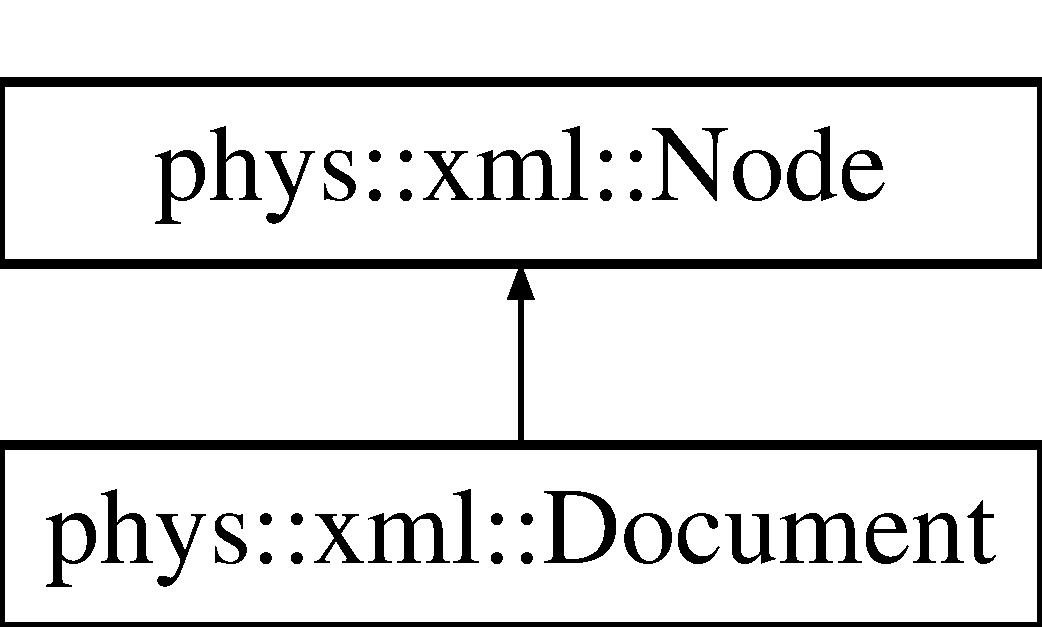
\includegraphics[height=2.000000cm]{d7/d0a/classphys_1_1xml_1_1Node}
\end{center}
\end{figure}
\subsection*{Public Types}
\begin{DoxyCompactItemize}
\item 
\hypertarget{classphys_1_1xml_1_1Node_a0da067636c89829a111dd51037cea6b3}{
typedef \hyperlink{classphys_1_1xml_1_1NodeIterator}{NodeIterator} {\bfseries iterator}}
\label{d7/d0a/classphys_1_1xml_1_1Node_a0da067636c89829a111dd51037cea6b3}

\item 
\hypertarget{classphys_1_1xml_1_1Node_a3b37ee9a716fc3a6cd92733ccf28f26a}{
typedef \hyperlink{classphys_1_1xml_1_1AttributeIterator}{AttributeIterator} {\bfseries attribute\_\-iterator}}
\label{d7/d0a/classphys_1_1xml_1_1Node_a3b37ee9a716fc3a6cd92733ccf28f26a}

\end{DoxyCompactItemize}
\subsection*{Public Member Functions}
\begin{DoxyCompactItemize}
\item 
\hypertarget{classphys_1_1xml_1_1Node_aaefbe98a05a7bf304612c3e7f7556f42}{
{\bfseries Node} (\hyperlink{structphys_1_1xml_1_1NodeStruct}{NodeStruct} $\ast$p)}
\label{d7/d0a/classphys_1_1xml_1_1Node_aaefbe98a05a7bf304612c3e7f7556f42}

\item 
\hypertarget{classphys_1_1xml_1_1Node_a1a3af56736ef4dd39596bb71607ebbc7}{
{\bfseries operator unspecified\_\-bool\_\-type} () const }
\label{d7/d0a/classphys_1_1xml_1_1Node_a1a3af56736ef4dd39596bb71607ebbc7}

\item 
\hypertarget{classphys_1_1xml_1_1Node_a121ff268fa51c4a66ad8d4a6734f4535}{
bool {\bfseries operator!} () const }
\label{d7/d0a/classphys_1_1xml_1_1Node_a121ff268fa51c4a66ad8d4a6734f4535}

\item 
\hypertarget{classphys_1_1xml_1_1Node_aa4008ce4f37c81ffc204198d9a026539}{
bool {\bfseries operator==} (const \hyperlink{classphys_1_1xml_1_1Node}{Node} \&r) const }
\label{d7/d0a/classphys_1_1xml_1_1Node_aa4008ce4f37c81ffc204198d9a026539}

\item 
\hypertarget{classphys_1_1xml_1_1Node_a00077491f468d40745a15963fc8c8bf7}{
bool {\bfseries operator!=} (const \hyperlink{classphys_1_1xml_1_1Node}{Node} \&r) const }
\label{d7/d0a/classphys_1_1xml_1_1Node_a00077491f468d40745a15963fc8c8bf7}

\item 
\hypertarget{classphys_1_1xml_1_1Node_ae60944f0610e55a12d772575a97e0e89}{
bool {\bfseries operator$<$} (const \hyperlink{classphys_1_1xml_1_1Node}{Node} \&r) const }
\label{d7/d0a/classphys_1_1xml_1_1Node_ae60944f0610e55a12d772575a97e0e89}

\item 
\hypertarget{classphys_1_1xml_1_1Node_a394f3b55158abd6716eeb8d7dd966262}{
bool {\bfseries operator$>$} (const \hyperlink{classphys_1_1xml_1_1Node}{Node} \&r) const }
\label{d7/d0a/classphys_1_1xml_1_1Node_a394f3b55158abd6716eeb8d7dd966262}

\item 
\hypertarget{classphys_1_1xml_1_1Node_a332214f0dddb3f70f4859dc13a3da09d}{
bool {\bfseries operator$<$=} (const \hyperlink{classphys_1_1xml_1_1Node}{Node} \&r) const }
\label{d7/d0a/classphys_1_1xml_1_1Node_a332214f0dddb3f70f4859dc13a3da09d}

\item 
\hypertarget{classphys_1_1xml_1_1Node_ac17b64d023f82a29048a01a97a60c681}{
bool {\bfseries operator$>$=} (const \hyperlink{classphys_1_1xml_1_1Node}{Node} \&r) const }
\label{d7/d0a/classphys_1_1xml_1_1Node_ac17b64d023f82a29048a01a97a60c681}

\item 
\hypertarget{classphys_1_1xml_1_1Node_aba1aa3acb0a4e824d27ea47e1ee6babb}{
bool {\bfseries empty} () const }
\label{d7/d0a/classphys_1_1xml_1_1Node_aba1aa3acb0a4e824d27ea47e1ee6babb}

\item 
\hypertarget{classphys_1_1xml_1_1Node_aeeab99e4798aa73cbdbafacf6cd3260b}{
\hyperlink{namespacephys_1_1xml_a668b0cc666a9d49f7c7222a7552115d3}{NodeType} {\bfseries type} () const }
\label{d7/d0a/classphys_1_1xml_1_1Node_aeeab99e4798aa73cbdbafacf6cd3260b}

\item 
\hypertarget{classphys_1_1xml_1_1Node_aad418ac3d573170a47dcc372ac03c2fd}{
const \hyperlink{namespacephys_1_1xml_afc87705cd1c2917d87b879715a2d8f6e}{char\_\-t} $\ast$ {\bfseries name} () const }
\label{d7/d0a/classphys_1_1xml_1_1Node_aad418ac3d573170a47dcc372ac03c2fd}

\item 
\hypertarget{classphys_1_1xml_1_1Node_a01319c62026515fa40beb2a4ad382e0a}{
const \hyperlink{namespacephys_1_1xml_afc87705cd1c2917d87b879715a2d8f6e}{char\_\-t} $\ast$ {\bfseries value} () const }
\label{d7/d0a/classphys_1_1xml_1_1Node_a01319c62026515fa40beb2a4ad382e0a}

\item 
\hypertarget{classphys_1_1xml_1_1Node_a1a7a7f8bd281438fbcdec154a45895df}{
\hyperlink{classphys_1_1xml_1_1Attribute}{Attribute} {\bfseries first\_\-attribute} () const }
\label{d7/d0a/classphys_1_1xml_1_1Node_a1a7a7f8bd281438fbcdec154a45895df}

\item 
\hypertarget{classphys_1_1xml_1_1Node_a58f0dec5e77665a2ffd30a48c7f9b341}{
\hyperlink{classphys_1_1xml_1_1Attribute}{Attribute} {\bfseries last\_\-attribute} () const }
\label{d7/d0a/classphys_1_1xml_1_1Node_a58f0dec5e77665a2ffd30a48c7f9b341}

\item 
\hypertarget{classphys_1_1xml_1_1Node_a0bd8c44af5a2e77fdd05e239a4d3c6f6}{
\hyperlink{classphys_1_1xml_1_1Node}{Node} {\bfseries first\_\-child} () const }
\label{d7/d0a/classphys_1_1xml_1_1Node_a0bd8c44af5a2e77fdd05e239a4d3c6f6}

\item 
\hypertarget{classphys_1_1xml_1_1Node_a2c0f2440aeb854bee7cbd79b16138a2c}{
\hyperlink{classphys_1_1xml_1_1Node}{Node} {\bfseries last\_\-child} () const }
\label{d7/d0a/classphys_1_1xml_1_1Node_a2c0f2440aeb854bee7cbd79b16138a2c}

\item 
\hypertarget{classphys_1_1xml_1_1Node_ae0b7a14f6984c141f7989c8298d33688}{
\hyperlink{classphys_1_1xml_1_1Node}{Node} {\bfseries next\_\-sibling} () const }
\label{d7/d0a/classphys_1_1xml_1_1Node_ae0b7a14f6984c141f7989c8298d33688}

\item 
\hypertarget{classphys_1_1xml_1_1Node_ac8fcf74064a8786a567559c3fc1bbc93}{
\hyperlink{classphys_1_1xml_1_1Node}{Node} {\bfseries previous\_\-sibling} () const }
\label{d7/d0a/classphys_1_1xml_1_1Node_ac8fcf74064a8786a567559c3fc1bbc93}

\item 
\hypertarget{classphys_1_1xml_1_1Node_a3588251e1a604c90869bb42419512272}{
\hyperlink{classphys_1_1xml_1_1Node}{Node} {\bfseries parent} () const }
\label{d7/d0a/classphys_1_1xml_1_1Node_a3588251e1a604c90869bb42419512272}

\item 
\hypertarget{classphys_1_1xml_1_1Node_a217f994285838f34c7d6d9464ff6effd}{
\hyperlink{classphys_1_1xml_1_1Node}{Node} {\bfseries root} () const }
\label{d7/d0a/classphys_1_1xml_1_1Node_a217f994285838f34c7d6d9464ff6effd}

\item 
\hypertarget{classphys_1_1xml_1_1Node_a227ad0bd82f6676660de3fbaea1890eb}{
\hyperlink{classphys_1_1xml_1_1Node}{Node} {\bfseries child} (const \hyperlink{namespacephys_1_1xml_afc87705cd1c2917d87b879715a2d8f6e}{char\_\-t} $\ast$name) const }
\label{d7/d0a/classphys_1_1xml_1_1Node_a227ad0bd82f6676660de3fbaea1890eb}

\item 
\hypertarget{classphys_1_1xml_1_1Node_a35ed5fae9a1286d5c08ec5819485c9da}{
\hyperlink{classphys_1_1xml_1_1Attribute}{Attribute} {\bfseries attribute} (const \hyperlink{namespacephys_1_1xml_afc87705cd1c2917d87b879715a2d8f6e}{char\_\-t} $\ast$name) const }
\label{d7/d0a/classphys_1_1xml_1_1Node_a35ed5fae9a1286d5c08ec5819485c9da}

\item 
\hypertarget{classphys_1_1xml_1_1Node_a682b97e4d5d7efcba0d790a92b75227d}{
\hyperlink{classphys_1_1xml_1_1Node}{Node} {\bfseries next\_\-sibling} (const \hyperlink{namespacephys_1_1xml_afc87705cd1c2917d87b879715a2d8f6e}{char\_\-t} $\ast$name) const }
\label{d7/d0a/classphys_1_1xml_1_1Node_a682b97e4d5d7efcba0d790a92b75227d}

\item 
\hypertarget{classphys_1_1xml_1_1Node_a7ec6a86fbf7f99afa11ac7e266e675d8}{
\hyperlink{classphys_1_1xml_1_1Node}{Node} {\bfseries previous\_\-sibling} (const \hyperlink{namespacephys_1_1xml_afc87705cd1c2917d87b879715a2d8f6e}{char\_\-t} $\ast$name) const }
\label{d7/d0a/classphys_1_1xml_1_1Node_a7ec6a86fbf7f99afa11ac7e266e675d8}

\item 
\hypertarget{classphys_1_1xml_1_1Node_aaa50cedf42226b2f3865f2dc5275b589}{
const \hyperlink{namespacephys_1_1xml_afc87705cd1c2917d87b879715a2d8f6e}{char\_\-t} $\ast$ {\bfseries child\_\-value} () const }
\label{d7/d0a/classphys_1_1xml_1_1Node_aaa50cedf42226b2f3865f2dc5275b589}

\item 
\hypertarget{classphys_1_1xml_1_1Node_a483a61a6ab2ccb84cb33a0228630b1c3}{
const \hyperlink{namespacephys_1_1xml_afc87705cd1c2917d87b879715a2d8f6e}{char\_\-t} $\ast$ {\bfseries child\_\-value} (const \hyperlink{namespacephys_1_1xml_afc87705cd1c2917d87b879715a2d8f6e}{char\_\-t} $\ast$name) const }
\label{d7/d0a/classphys_1_1xml_1_1Node_a483a61a6ab2ccb84cb33a0228630b1c3}

\item 
\hypertarget{classphys_1_1xml_1_1Node_aa8c259aaaf405d9332130f40ca6679fc}{
bool {\bfseries set\_\-name} (const \hyperlink{namespacephys_1_1xml_afc87705cd1c2917d87b879715a2d8f6e}{char\_\-t} $\ast$rhs)}
\label{d7/d0a/classphys_1_1xml_1_1Node_aa8c259aaaf405d9332130f40ca6679fc}

\item 
\hypertarget{classphys_1_1xml_1_1Node_a765ff43292ade8e24c5b7b2808f3c7de}{
bool {\bfseries set\_\-value} (const \hyperlink{namespacephys_1_1xml_afc87705cd1c2917d87b879715a2d8f6e}{char\_\-t} $\ast$rhs)}
\label{d7/d0a/classphys_1_1xml_1_1Node_a765ff43292ade8e24c5b7b2808f3c7de}

\item 
\hypertarget{classphys_1_1xml_1_1Node_a33b7c276f62e0c25ff7833a897888125}{
\hyperlink{classphys_1_1xml_1_1Attribute}{Attribute} {\bfseries append\_\-attribute} (const \hyperlink{namespacephys_1_1xml_afc87705cd1c2917d87b879715a2d8f6e}{char\_\-t} $\ast$name)}
\label{d7/d0a/classphys_1_1xml_1_1Node_a33b7c276f62e0c25ff7833a897888125}

\item 
\hypertarget{classphys_1_1xml_1_1Node_abc20afab0e50b0d9c578a02e91608226}{
\hyperlink{classphys_1_1xml_1_1Attribute}{Attribute} {\bfseries prepend\_\-attribute} (const \hyperlink{namespacephys_1_1xml_afc87705cd1c2917d87b879715a2d8f6e}{char\_\-t} $\ast$name)}
\label{d7/d0a/classphys_1_1xml_1_1Node_abc20afab0e50b0d9c578a02e91608226}

\item 
\hypertarget{classphys_1_1xml_1_1Node_aae7d7e21d419c9f95549d14ddccb1334}{
\hyperlink{classphys_1_1xml_1_1Attribute}{Attribute} {\bfseries insert\_\-attribute\_\-after} (const \hyperlink{namespacephys_1_1xml_afc87705cd1c2917d87b879715a2d8f6e}{char\_\-t} $\ast$name, const \hyperlink{classphys_1_1xml_1_1Attribute}{Attribute} \&attr)}
\label{d7/d0a/classphys_1_1xml_1_1Node_aae7d7e21d419c9f95549d14ddccb1334}

\item 
\hypertarget{classphys_1_1xml_1_1Node_a0b22783a8ce773f7b3847d7f2ec9b475}{
\hyperlink{classphys_1_1xml_1_1Attribute}{Attribute} {\bfseries insert\_\-attribute\_\-before} (const \hyperlink{namespacephys_1_1xml_afc87705cd1c2917d87b879715a2d8f6e}{char\_\-t} $\ast$name, const \hyperlink{classphys_1_1xml_1_1Attribute}{Attribute} \&attr)}
\label{d7/d0a/classphys_1_1xml_1_1Node_a0b22783a8ce773f7b3847d7f2ec9b475}

\item 
\hypertarget{classphys_1_1xml_1_1Node_a8067d9c5861a4dc89c644eded1987b7d}{
\hyperlink{classphys_1_1xml_1_1Attribute}{Attribute} {\bfseries append\_\-copy} (const \hyperlink{classphys_1_1xml_1_1Attribute}{Attribute} \&proto)}
\label{d7/d0a/classphys_1_1xml_1_1Node_a8067d9c5861a4dc89c644eded1987b7d}

\item 
\hypertarget{classphys_1_1xml_1_1Node_a875eb8b249394050178e26d978a247cf}{
\hyperlink{classphys_1_1xml_1_1Attribute}{Attribute} {\bfseries prepend\_\-copy} (const \hyperlink{classphys_1_1xml_1_1Attribute}{Attribute} \&proto)}
\label{d7/d0a/classphys_1_1xml_1_1Node_a875eb8b249394050178e26d978a247cf}

\item 
\hypertarget{classphys_1_1xml_1_1Node_a0d12c7f719d26042afb83b8045babbf0}{
\hyperlink{classphys_1_1xml_1_1Attribute}{Attribute} {\bfseries insert\_\-copy\_\-after} (const \hyperlink{classphys_1_1xml_1_1Attribute}{Attribute} \&proto, const \hyperlink{classphys_1_1xml_1_1Attribute}{Attribute} \&attr)}
\label{d7/d0a/classphys_1_1xml_1_1Node_a0d12c7f719d26042afb83b8045babbf0}

\item 
\hypertarget{classphys_1_1xml_1_1Node_af4b5824124e70eda957c410e66123896}{
\hyperlink{classphys_1_1xml_1_1Attribute}{Attribute} {\bfseries insert\_\-copy\_\-before} (const \hyperlink{classphys_1_1xml_1_1Attribute}{Attribute} \&proto, const \hyperlink{classphys_1_1xml_1_1Attribute}{Attribute} \&attr)}
\label{d7/d0a/classphys_1_1xml_1_1Node_af4b5824124e70eda957c410e66123896}

\item 
\hypertarget{classphys_1_1xml_1_1Node_af2601376ae30b9744b3b10067d26de9a}{
\hyperlink{classphys_1_1xml_1_1Node}{Node} {\bfseries append\_\-child} (\hyperlink{namespacephys_1_1xml_a668b0cc666a9d49f7c7222a7552115d3}{NodeType} type=NodeElement)}
\label{d7/d0a/classphys_1_1xml_1_1Node_af2601376ae30b9744b3b10067d26de9a}

\item 
\hypertarget{classphys_1_1xml_1_1Node_ae34bde1d0157fe19996c26099a22695c}{
\hyperlink{classphys_1_1xml_1_1Node}{Node} {\bfseries prepend\_\-child} (\hyperlink{namespacephys_1_1xml_a668b0cc666a9d49f7c7222a7552115d3}{NodeType} type=NodeElement)}
\label{d7/d0a/classphys_1_1xml_1_1Node_ae34bde1d0157fe19996c26099a22695c}

\item 
\hypertarget{classphys_1_1xml_1_1Node_a6c6b4225db38e4f031ee68d5c8c86377}{
\hyperlink{classphys_1_1xml_1_1Node}{Node} {\bfseries insert\_\-child\_\-after} (\hyperlink{namespacephys_1_1xml_a668b0cc666a9d49f7c7222a7552115d3}{NodeType} type, const \hyperlink{classphys_1_1xml_1_1Node}{Node} \&node)}
\label{d7/d0a/classphys_1_1xml_1_1Node_a6c6b4225db38e4f031ee68d5c8c86377}

\item 
\hypertarget{classphys_1_1xml_1_1Node_a36dd60f74bcf0ac054169c3c6ae8e286}{
\hyperlink{classphys_1_1xml_1_1Node}{Node} {\bfseries insert\_\-child\_\-before} (\hyperlink{namespacephys_1_1xml_a668b0cc666a9d49f7c7222a7552115d3}{NodeType} type, const \hyperlink{classphys_1_1xml_1_1Node}{Node} \&node)}
\label{d7/d0a/classphys_1_1xml_1_1Node_a36dd60f74bcf0ac054169c3c6ae8e286}

\item 
\hypertarget{classphys_1_1xml_1_1Node_aae3d925cc040d9fddfe173410bcdd322}{
\hyperlink{classphys_1_1xml_1_1Node}{Node} {\bfseries append\_\-child} (const \hyperlink{namespacephys_1_1xml_afc87705cd1c2917d87b879715a2d8f6e}{char\_\-t} $\ast$name)}
\label{d7/d0a/classphys_1_1xml_1_1Node_aae3d925cc040d9fddfe173410bcdd322}

\item 
\hypertarget{classphys_1_1xml_1_1Node_ab6e8a5ec035a2b66a3d0475498012f3d}{
\hyperlink{classphys_1_1xml_1_1Node}{Node} {\bfseries prepend\_\-child} (const \hyperlink{namespacephys_1_1xml_afc87705cd1c2917d87b879715a2d8f6e}{char\_\-t} $\ast$name)}
\label{d7/d0a/classphys_1_1xml_1_1Node_ab6e8a5ec035a2b66a3d0475498012f3d}

\item 
\hypertarget{classphys_1_1xml_1_1Node_a6b3345a4e9f56147c21c76a8aeb5d9df}{
\hyperlink{classphys_1_1xml_1_1Node}{Node} {\bfseries insert\_\-child\_\-after} (const \hyperlink{namespacephys_1_1xml_afc87705cd1c2917d87b879715a2d8f6e}{char\_\-t} $\ast$name, const \hyperlink{classphys_1_1xml_1_1Node}{Node} \&node)}
\label{d7/d0a/classphys_1_1xml_1_1Node_a6b3345a4e9f56147c21c76a8aeb5d9df}

\item 
\hypertarget{classphys_1_1xml_1_1Node_a9212a51ca71f8098b5425bb459eb366c}{
\hyperlink{classphys_1_1xml_1_1Node}{Node} {\bfseries insert\_\-child\_\-before} (const \hyperlink{namespacephys_1_1xml_afc87705cd1c2917d87b879715a2d8f6e}{char\_\-t} $\ast$name, const \hyperlink{classphys_1_1xml_1_1Node}{Node} \&node)}
\label{d7/d0a/classphys_1_1xml_1_1Node_a9212a51ca71f8098b5425bb459eb366c}

\item 
\hypertarget{classphys_1_1xml_1_1Node_a0bf9542120cadd27890fa60aa365a849}{
\hyperlink{classphys_1_1xml_1_1Node}{Node} {\bfseries append\_\-copy} (const \hyperlink{classphys_1_1xml_1_1Node}{Node} \&proto)}
\label{d7/d0a/classphys_1_1xml_1_1Node_a0bf9542120cadd27890fa60aa365a849}

\item 
\hypertarget{classphys_1_1xml_1_1Node_a96508d5e780085b962263c093dcb1e27}{
\hyperlink{classphys_1_1xml_1_1Node}{Node} {\bfseries prepend\_\-copy} (const \hyperlink{classphys_1_1xml_1_1Node}{Node} \&proto)}
\label{d7/d0a/classphys_1_1xml_1_1Node_a96508d5e780085b962263c093dcb1e27}

\item 
\hypertarget{classphys_1_1xml_1_1Node_a0620e8a5196afc37694f5385e639d006}{
\hyperlink{classphys_1_1xml_1_1Node}{Node} {\bfseries insert\_\-copy\_\-after} (const \hyperlink{classphys_1_1xml_1_1Node}{Node} \&proto, const \hyperlink{classphys_1_1xml_1_1Node}{Node} \&node)}
\label{d7/d0a/classphys_1_1xml_1_1Node_a0620e8a5196afc37694f5385e639d006}

\item 
\hypertarget{classphys_1_1xml_1_1Node_a80828f043fc136104b602126cfc566a5}{
\hyperlink{classphys_1_1xml_1_1Node}{Node} {\bfseries insert\_\-copy\_\-before} (const \hyperlink{classphys_1_1xml_1_1Node}{Node} \&proto, const \hyperlink{classphys_1_1xml_1_1Node}{Node} \&node)}
\label{d7/d0a/classphys_1_1xml_1_1Node_a80828f043fc136104b602126cfc566a5}

\item 
\hypertarget{classphys_1_1xml_1_1Node_a99699d6740844fd73bd4704c954a222d}{
bool {\bfseries remove\_\-attribute} (const \hyperlink{classphys_1_1xml_1_1Attribute}{Attribute} \&a)}
\label{d7/d0a/classphys_1_1xml_1_1Node_a99699d6740844fd73bd4704c954a222d}

\item 
\hypertarget{classphys_1_1xml_1_1Node_a070ffe875695188e68f0554cd2efc2a9}{
bool {\bfseries remove\_\-attribute} (const \hyperlink{namespacephys_1_1xml_afc87705cd1c2917d87b879715a2d8f6e}{char\_\-t} $\ast$name)}
\label{d7/d0a/classphys_1_1xml_1_1Node_a070ffe875695188e68f0554cd2efc2a9}

\item 
\hypertarget{classphys_1_1xml_1_1Node_a2cf35b26227f6067a25a2ae1647e8f31}{
bool {\bfseries remove\_\-child} (const \hyperlink{classphys_1_1xml_1_1Node}{Node} \&n)}
\label{d7/d0a/classphys_1_1xml_1_1Node_a2cf35b26227f6067a25a2ae1647e8f31}

\item 
\hypertarget{classphys_1_1xml_1_1Node_ab10af5783c31fb58cc533b58a3c11ae0}{
bool {\bfseries remove\_\-child} (const \hyperlink{namespacephys_1_1xml_afc87705cd1c2917d87b879715a2d8f6e}{char\_\-t} $\ast$name)}
\label{d7/d0a/classphys_1_1xml_1_1Node_ab10af5783c31fb58cc533b58a3c11ae0}

\item 
\hypertarget{classphys_1_1xml_1_1Node_a59e43a51c83065e02fea2f39a37d84f0}{
{\footnotesize template$<$typename Predicate $>$ }\\\hyperlink{classphys_1_1xml_1_1Attribute}{Attribute} {\bfseries find\_\-attribute} (Predicate pred) const }
\label{d7/d0a/classphys_1_1xml_1_1Node_a59e43a51c83065e02fea2f39a37d84f0}

\item 
\hypertarget{classphys_1_1xml_1_1Node_aa46f1a55d5fead8ea4cc68235e45f3fc}{
{\footnotesize template$<$typename Predicate $>$ }\\\hyperlink{classphys_1_1xml_1_1Node}{Node} {\bfseries find\_\-child} (Predicate pred) const }
\label{d7/d0a/classphys_1_1xml_1_1Node_aa46f1a55d5fead8ea4cc68235e45f3fc}

\item 
\hypertarget{classphys_1_1xml_1_1Node_af755f4925f6839e0f8a768cfc3b265d4}{
{\footnotesize template$<$typename Predicate $>$ }\\\hyperlink{classphys_1_1xml_1_1Node}{Node} {\bfseries find\_\-node} (Predicate pred) const }
\label{d7/d0a/classphys_1_1xml_1_1Node_af755f4925f6839e0f8a768cfc3b265d4}

\item 
\hypertarget{classphys_1_1xml_1_1Node_ad877293c5bfd97ea7f4e6319db816ac4}{
\hyperlink{classphys_1_1xml_1_1Node}{Node} {\bfseries find\_\-child\_\-by\_\-attribute} (const \hyperlink{namespacephys_1_1xml_afc87705cd1c2917d87b879715a2d8f6e}{char\_\-t} $\ast$name, const \hyperlink{namespacephys_1_1xml_afc87705cd1c2917d87b879715a2d8f6e}{char\_\-t} $\ast$attr\_\-name, const \hyperlink{namespacephys_1_1xml_afc87705cd1c2917d87b879715a2d8f6e}{char\_\-t} $\ast$attr\_\-value) const }
\label{d7/d0a/classphys_1_1xml_1_1Node_ad877293c5bfd97ea7f4e6319db816ac4}

\item 
\hypertarget{classphys_1_1xml_1_1Node_aa3ea620c51e0af54aebcf78586086a9a}{
\hyperlink{classphys_1_1xml_1_1Node}{Node} {\bfseries find\_\-child\_\-by\_\-attribute} (const \hyperlink{namespacephys_1_1xml_afc87705cd1c2917d87b879715a2d8f6e}{char\_\-t} $\ast$attr\_\-name, const \hyperlink{namespacephys_1_1xml_afc87705cd1c2917d87b879715a2d8f6e}{char\_\-t} $\ast$attr\_\-value) const }
\label{d7/d0a/classphys_1_1xml_1_1Node_aa3ea620c51e0af54aebcf78586086a9a}

\item 
\hypertarget{classphys_1_1xml_1_1Node_a74b9f51a6642808510e71f643cc861ad}{
\hyperlink{namespacephys_1_1xml_a6db751f2b35502e04c123bb70daa0d20}{string\_\-t} {\bfseries path} (\hyperlink{namespacephys_1_1xml_afc87705cd1c2917d87b879715a2d8f6e}{char\_\-t} delimiter= '/') const }
\label{d7/d0a/classphys_1_1xml_1_1Node_a74b9f51a6642808510e71f643cc861ad}

\item 
\hypertarget{classphys_1_1xml_1_1Node_ad771e6d5faca7c608a6a6cd1e29dd3d8}{
\hyperlink{classphys_1_1xml_1_1Node}{Node} {\bfseries first\_\-element\_\-by\_\-path} (const \hyperlink{namespacephys_1_1xml_afc87705cd1c2917d87b879715a2d8f6e}{char\_\-t} $\ast$path, \hyperlink{namespacephys_1_1xml_afc87705cd1c2917d87b879715a2d8f6e}{char\_\-t} delimiter= '/') const }
\label{d7/d0a/classphys_1_1xml_1_1Node_ad771e6d5faca7c608a6a6cd1e29dd3d8}

\item 
\hypertarget{classphys_1_1xml_1_1Node_abf6c5b96ced5404a204a4700f044f982}{
bool {\bfseries traverse} (\hyperlink{classphys_1_1xml_1_1TreeWalker}{TreeWalker} \&walker)}
\label{d7/d0a/classphys_1_1xml_1_1Node_abf6c5b96ced5404a204a4700f044f982}

\item 
\hypertarget{classphys_1_1xml_1_1Node_ad3caa2f4cafd56c79000a5af848f3e62}{
\hyperlink{classphys_1_1xml_1_1XPathNode}{XPathNode} {\bfseries select\_\-single\_\-node} (const \hyperlink{namespacephys_1_1xml_afc87705cd1c2917d87b879715a2d8f6e}{char\_\-t} $\ast$query, \hyperlink{classphys_1_1xml_1_1XPathVariableSet}{XPathVariableSet} $\ast$variables=0) const }
\label{d7/d0a/classphys_1_1xml_1_1Node_ad3caa2f4cafd56c79000a5af848f3e62}

\item 
\hypertarget{classphys_1_1xml_1_1Node_a599ed26773b23999c6f2e87e76deb0fd}{
\hyperlink{classphys_1_1xml_1_1XPathNode}{XPathNode} {\bfseries select\_\-single\_\-node} (const \hyperlink{classphys_1_1xml_1_1XPathQuery}{XPathQuery} \&query) const }
\label{d7/d0a/classphys_1_1xml_1_1Node_a599ed26773b23999c6f2e87e76deb0fd}

\item 
\hypertarget{classphys_1_1xml_1_1Node_ad8bc358815511c63677a60149fe9a6dd}{
\hyperlink{classphys_1_1xml_1_1XPathNodeSet}{XPathNodeSet} {\bfseries select\_\-nodes} (const \hyperlink{namespacephys_1_1xml_afc87705cd1c2917d87b879715a2d8f6e}{char\_\-t} $\ast$query, \hyperlink{classphys_1_1xml_1_1XPathVariableSet}{XPathVariableSet} $\ast$variables=0) const }
\label{d7/d0a/classphys_1_1xml_1_1Node_ad8bc358815511c63677a60149fe9a6dd}

\item 
\hypertarget{classphys_1_1xml_1_1Node_ae1e232d5d010ca9272edd7bbe3154b44}{
\hyperlink{classphys_1_1xml_1_1XPathNodeSet}{XPathNodeSet} {\bfseries select\_\-nodes} (const \hyperlink{classphys_1_1xml_1_1XPathQuery}{XPathQuery} \&query) const }
\label{d7/d0a/classphys_1_1xml_1_1Node_ae1e232d5d010ca9272edd7bbe3154b44}

\item 
\hypertarget{classphys_1_1xml_1_1Node_a526817671e39653b0dca70c2ba8daa55}{
void {\bfseries print} (\hyperlink{classphys_1_1xml_1_1Writer}{Writer} \&WriterInstance, const \hyperlink{namespacephys_1_1xml_afc87705cd1c2917d87b879715a2d8f6e}{char\_\-t} $\ast$indent=XML\_\-TEXT(\char`\"{}$\backslash$t\char`\"{}), unsigned int flags=\hyperlink{namespacephys_1_1xml_a08bf6aab51f79929d9097706a5e64408}{FormatDefault}, \hyperlink{namespacephys_1_1xml_a420f5de782438f88160321385bea2015}{Encoding} DocumentEncoding=EncodingAuto, unsigned int depth=0) const }
\label{d7/d0a/classphys_1_1xml_1_1Node_a526817671e39653b0dca70c2ba8daa55}

\item 
\hypertarget{classphys_1_1xml_1_1Node_a99158a08970f0497a3925dddf8227b87}{
void {\bfseries print} (std::basic\_\-ostream$<$ char, std::char\_\-traits$<$ char $>$ $>$ \&os, const \hyperlink{namespacephys_1_1xml_afc87705cd1c2917d87b879715a2d8f6e}{char\_\-t} $\ast$indent=XML\_\-TEXT(\char`\"{}$\backslash$t\char`\"{}), unsigned int flags=\hyperlink{namespacephys_1_1xml_a08bf6aab51f79929d9097706a5e64408}{FormatDefault}, \hyperlink{namespacephys_1_1xml_a420f5de782438f88160321385bea2015}{Encoding} DocumentEncoding=EncodingAuto, unsigned int depth=0) const }
\label{d7/d0a/classphys_1_1xml_1_1Node_a99158a08970f0497a3925dddf8227b87}

\item 
\hypertarget{classphys_1_1xml_1_1Node_a27b7869e5208547e06b6164bbc68ca0e}{
void {\bfseries print} (std::basic\_\-ostream$<$ wchar\_\-t, std::char\_\-traits$<$ wchar\_\-t $>$ $>$ \&os, const \hyperlink{namespacephys_1_1xml_afc87705cd1c2917d87b879715a2d8f6e}{char\_\-t} $\ast$indent=XML\_\-TEXT(\char`\"{}$\backslash$t\char`\"{}), unsigned int flags=\hyperlink{namespacephys_1_1xml_a08bf6aab51f79929d9097706a5e64408}{FormatDefault}, unsigned int depth=0) const }
\label{d7/d0a/classphys_1_1xml_1_1Node_a27b7869e5208547e06b6164bbc68ca0e}

\item 
\hypertarget{classphys_1_1xml_1_1Node_a78c82f35dcf7b2c37f1f5ff37d526329}{
\hyperlink{classphys_1_1xml_1_1NodeIterator}{iterator} {\bfseries begin} () const }
\label{d7/d0a/classphys_1_1xml_1_1Node_a78c82f35dcf7b2c37f1f5ff37d526329}

\item 
\hypertarget{classphys_1_1xml_1_1Node_ae69ca8be6e9eb53a4faf8bb50a2996d6}{
\hyperlink{classphys_1_1xml_1_1NodeIterator}{iterator} {\bfseries end} () const }
\label{d7/d0a/classphys_1_1xml_1_1Node_ae69ca8be6e9eb53a4faf8bb50a2996d6}

\item 
\hypertarget{classphys_1_1xml_1_1Node_a601285bed116eb5d63cea9a8d117e5b7}{
\hyperlink{classphys_1_1xml_1_1AttributeIterator}{attribute\_\-iterator} {\bfseries attributes\_\-begin} () const }
\label{d7/d0a/classphys_1_1xml_1_1Node_a601285bed116eb5d63cea9a8d117e5b7}

\item 
\hypertarget{classphys_1_1xml_1_1Node_a9af9e0bff5b8ed06bc40861dccb6b4ec}{
\hyperlink{classphys_1_1xml_1_1AttributeIterator}{attribute\_\-iterator} {\bfseries attributes\_\-end} () const }
\label{d7/d0a/classphys_1_1xml_1_1Node_a9af9e0bff5b8ed06bc40861dccb6b4ec}

\item 
\hypertarget{classphys_1_1xml_1_1Node_a6439833c334aa4d4dd3032609d697497}{
ptrdiff\_\-t {\bfseries Offset\_\-debug} () const }
\label{d7/d0a/classphys_1_1xml_1_1Node_a6439833c334aa4d4dd3032609d697497}

\item 
\hypertarget{classphys_1_1xml_1_1Node_ad759e1e8c2c131e7ed438ce6308fd79b}{
size\_\-t {\bfseries hash\_\-value} () const }
\label{d7/d0a/classphys_1_1xml_1_1Node_ad759e1e8c2c131e7ed438ce6308fd79b}

\item 
\hypertarget{classphys_1_1xml_1_1Node_a911d3691004d14cb60dcefbe85c41046}{
\hyperlink{structphys_1_1xml_1_1NodeStruct}{NodeStruct} $\ast$ {\bfseries internal\_\-object} () const }
\label{d7/d0a/classphys_1_1xml_1_1Node_a911d3691004d14cb60dcefbe85c41046}

\end{DoxyCompactItemize}
\subsection*{Protected Types}
\begin{DoxyCompactItemize}
\item 
\hypertarget{classphys_1_1xml_1_1Node_abace2c2c7e70431d920579917417c1e4}{
typedef \hyperlink{structphys_1_1xml_1_1NodeStruct}{NodeStruct} $\ast$Node::$\ast$ {\bfseries unspecified\_\-bool\_\-type}}
\label{d7/d0a/classphys_1_1xml_1_1Node_abace2c2c7e70431d920579917417c1e4}

\end{DoxyCompactItemize}
\subsection*{Protected Attributes}
\begin{DoxyCompactItemize}
\item 
\hypertarget{classphys_1_1xml_1_1Node_ae76db7e7025e29af83e487cf4b270424}{
\hyperlink{structphys_1_1xml_1_1NodeStruct}{NodeStruct} $\ast$ {\bfseries \_\-root}}
\label{d7/d0a/classphys_1_1xml_1_1Node_ae76db7e7025e29af83e487cf4b270424}

\end{DoxyCompactItemize}
\subsection*{Friends}
\begin{DoxyCompactItemize}
\item 
\hypertarget{classphys_1_1xml_1_1Node_a1ed8790083a80b2604beba1c666bce6e}{
class {\bfseries AttributeIterator}}
\label{d7/d0a/classphys_1_1xml_1_1Node_a1ed8790083a80b2604beba1c666bce6e}

\item 
\hypertarget{classphys_1_1xml_1_1Node_ac5a1d2c6036b7ba1894a7c3b8d96a312}{
class {\bfseries NodeIterator}}
\label{d7/d0a/classphys_1_1xml_1_1Node_ac5a1d2c6036b7ba1894a7c3b8d96a312}

\end{DoxyCompactItemize}


\subsection{Detailed Description}


Definition at line 419 of file xml.h.



The documentation for this class was generated from the following files:\begin{DoxyCompactItemize}
\item 
\hyperlink{xml_8h}{xml.h}\item 
xml.cpp\end{DoxyCompactItemize}

\hypertarget{classphys_1_1Node}{
\section{phys::Node Class Reference}
\label{d0/ddc/classphys_1_1Node}\index{phys::Node@{phys::Node}}
}


This is a helper class which non-\/physics objects, such as lights, cameras, ribbon trails, and particle effects may be attached to for enhanced effects.  




{\ttfamily \#include $<$node.h$>$}

\subsection*{Public Types}
\begin{DoxyCompactItemize}
\item 
enum {\bfseries NodeType} \{ {\bfseries Center}, 
{\bfseries Orbit}, 
{\bfseries Stand}, 
{\bfseries Free}
 \}
\end{DoxyCompactItemize}
\subsection*{Public Member Functions}
\begin{DoxyCompactItemize}
\item 
\hyperlink{classphys_1_1Node_a09393f483ab4bb2fdb74b26a59ffd37e}{Node} (const \hyperlink{namespacephys_aa03900411993de7fbfec4789bc1d392e}{String} \&Name, \hyperlink{classphys_1_1SceneManager}{SceneManager} $\ast$manager)
\begin{DoxyCompactList}\small\item\em Standard initialization constructor. \item\end{DoxyCompactList}\item 
\hyperlink{classphys_1_1Node_af0f42610cf0adcef9e4dea16013cbaf2}{Node} (Ogre::SceneNode $\ast$snode, \hyperlink{classphys_1_1SceneManager}{SceneManager} $\ast$manager)
\begin{DoxyCompactList}\small\item\em Internal constructor. \item\end{DoxyCompactList}\item 
\hypertarget{classphys_1_1Node_af933598679e73d1e440f264f83e9d563}{
\hyperlink{classphys_1_1Node_af933598679e73d1e440f264f83e9d563}{$\sim$Node} ()}
\label{d0/ddc/classphys_1_1Node_af933598679e73d1e440f264f83e9d563}

\begin{DoxyCompactList}\small\item\em Class destructor. \item\end{DoxyCompactList}\item 
\hyperlink{namespacephys_a5ce5049f8b4bf88d6413c47b504ebb31}{ConstString} \& \hyperlink{classphys_1_1Node_a2db8f0717abc20a43b7154bdc99ecf0e}{GetName} ()
\begin{DoxyCompactList}\small\item\em Gets the name of this node. \item\end{DoxyCompactList}\item 
void \hyperlink{classphys_1_1Node_a8de0f86b08510a08a6e6c0912c9caddb}{AttachElement} (\hyperlink{classphys_1_1Attachable}{Attachable} $\ast$Element)
\begin{DoxyCompactList}\small\item\em Attaches an attachable element to this \hyperlink{classphys_1_1Node}{Node}. \item\end{DoxyCompactList}\item 
void \hyperlink{classphys_1_1Node_afdafaa00a4c6873211968529993a2b48}{DetachElement} (\hyperlink{classphys_1_1Attachable}{Attachable} $\ast$Element)
\begin{DoxyCompactList}\small\item\em Detaches an attachable element from this \hyperlink{classphys_1_1Node}{Node}. \item\end{DoxyCompactList}\item 
\hypertarget{classphys_1_1Node_a8c0da465ac3b751cd4c124bf3157ce6b}{
void \hyperlink{classphys_1_1Node_a8c0da465ac3b751cd4c124bf3157ce6b}{DetachAllElements} ()}
\label{d0/ddc/classphys_1_1Node_a8c0da465ac3b751cd4c124bf3157ce6b}

\begin{DoxyCompactList}\small\item\em Detaches all attached cameras, lights, and particle effects. \item\end{DoxyCompactList}\item 
\hyperlink{namespacephys_a460f6bc24c8dd347b05e0366ae34f34a}{Whole} \hyperlink{classphys_1_1Node_ae4ee282575f7b1e6bb9dfcda15fcfd47}{GetNumAttachedElements} ()
\begin{DoxyCompactList}\small\item\em Gets the number of elements attached to this node. \item\end{DoxyCompactList}\item 
void \hyperlink{classphys_1_1Node_ab8dc3aa58292b0156e67dc3684099bbe}{SetPosition} (\hyperlink{classphys_1_1Vector3}{Vector3} Position)
\begin{DoxyCompactList}\small\item\em Sets the position of this node. \item\end{DoxyCompactList}\item 
\hyperlink{classphys_1_1Vector3}{Vector3} \hyperlink{classphys_1_1Node_adbb895705afa97bd5d824f0abf59e11a}{GetPosition} ()
\begin{DoxyCompactList}\small\item\em Gets the position of this node. \item\end{DoxyCompactList}\item 
void \hyperlink{classphys_1_1Node_a3799cc7b685a4bbbb16b6f9b917824a8}{SetOrientation} (\hyperlink{classphys_1_1Quaternion}{Quaternion} Orientation)
\begin{DoxyCompactList}\small\item\em Sets the orientation of this node. \item\end{DoxyCompactList}\item 
\hyperlink{classphys_1_1Quaternion}{Quaternion} \hyperlink{classphys_1_1Node_af9bda096f298c0ae692d52dd3b7c3733}{GetOrientation} ()
\begin{DoxyCompactList}\small\item\em Gets the orientation of this node. \item\end{DoxyCompactList}\item 
void \hyperlink{classphys_1_1Node_a545f5696660b3e7c07154b29421ab179}{LookAt} (\hyperlink{classphys_1_1Vector3}{Vector3} LookAt)
\begin{DoxyCompactList}\small\item\em Automatically sets the orientation needed to point this node at a location in the world. \item\end{DoxyCompactList}\item 
void \hyperlink{classphys_1_1Node_a0e652a52ea7d6e18280d1fc4b283c86a}{SetAutoTracking} (\hyperlink{classphys_1_1Node}{Node} $\ast$node, \hyperlink{classphys_1_1Vector3}{Vector3} Offset=\hyperlink{classphys_1_1Vector3}{Vector3}())
\begin{DoxyCompactList}\small\item\em Makes this node autotrack another node. \item\end{DoxyCompactList}\item 
void \hyperlink{classphys_1_1Node_adc570391b491821a13b58e15e0dc2cac}{SetAutoTracking} (\hyperlink{classphys_1_1ActorBase}{ActorBase} $\ast$Actor, \hyperlink{classphys_1_1Vector3}{Vector3} Offset=\hyperlink{classphys_1_1Vector3}{Vector3}())
\begin{DoxyCompactList}\small\item\em Makes this node autotrack an actor. \item\end{DoxyCompactList}\item 
\hypertarget{classphys_1_1Node_a5571ede65a6edf20788700b5d408bf04}{
void \hyperlink{classphys_1_1Node_a5571ede65a6edf20788700b5d408bf04}{DisableAutoTracking} ()}
\label{d0/ddc/classphys_1_1Node_a5571ede65a6edf20788700b5d408bf04}

\begin{DoxyCompactList}\small\item\em Disables any active autotracking for this node. \item\end{DoxyCompactList}\item 
void \hyperlink{classphys_1_1Node_a93fbb2b20f3cab180f7bdd39299c252e}{IncrementOrbit} (\hyperlink{namespacephys_af7eb897198d265b8e868f45240230d5f}{Real} Radians)
\begin{DoxyCompactList}\small\item\em Increments the orbit of this node if this is an orbiting node. \item\end{DoxyCompactList}\item 
void \hyperlink{classphys_1_1Node_afbc58e8c751f617c89a2246c397c679e}{SetType} (Node::NodeType type)
\begin{DoxyCompactList}\small\item\em Sets the type of node that this is. \item\end{DoxyCompactList}\item 
Node::NodeType \hyperlink{classphys_1_1Node_aee8632b4db2accd810afd096247252c2}{GetType} ()
\begin{DoxyCompactList}\small\item\em Gets the type of node that this is. \item\end{DoxyCompactList}\end{DoxyCompactItemize}
\subsection*{Protected Attributes}
\begin{DoxyCompactItemize}
\item 
\hypertarget{classphys_1_1Node_ad3206b5ec36cb374e01cb8e822616c45}{
Ogre::SceneNode $\ast$ \hyperlink{classphys_1_1Node_ad3206b5ec36cb374e01cb8e822616c45}{OgreNode}}
\label{d0/ddc/classphys_1_1Node_ad3206b5ec36cb374e01cb8e822616c45}

\begin{DoxyCompactList}\small\item\em Pointer to the ogre scenenode from which this class gets it's functionality. \item\end{DoxyCompactList}\item 
\hypertarget{classphys_1_1Node_a7bb7fd7fc172f155d205512ef65f62a8}{
\hyperlink{classphys_1_1SceneManager}{SceneManager} $\ast$ \hyperlink{classphys_1_1Node_a7bb7fd7fc172f155d205512ef65f62a8}{Manager}}
\label{d0/ddc/classphys_1_1Node_a7bb7fd7fc172f155d205512ef65f62a8}

\begin{DoxyCompactList}\small\item\em Pointer to the manager that created this class. \item\end{DoxyCompactList}\item 
\hypertarget{classphys_1_1Node_a25ef0ab80e0dc257ecc3d3ce38f3236d}{
Node::NodeType \hyperlink{classphys_1_1Node_a25ef0ab80e0dc257ecc3d3ce38f3236d}{Type}}
\label{d0/ddc/classphys_1_1Node_a25ef0ab80e0dc257ecc3d3ce38f3236d}

\begin{DoxyCompactList}\small\item\em Enum value storing the type of node this class is. \item\end{DoxyCompactList}\item 
\hypertarget{classphys_1_1Node_a98c80724ecec3696aaa4c50574b522b4}{
std::vector$<$ \hyperlink{classphys_1_1Attachable}{Attachable} $\ast$ $>$ \hyperlink{classphys_1_1Node_a98c80724ecec3696aaa4c50574b522b4}{Elements}}
\label{d0/ddc/classphys_1_1Node_a98c80724ecec3696aaa4c50574b522b4}

\begin{DoxyCompactList}\small\item\em Vector storing all attached cameras. \item\end{DoxyCompactList}\end{DoxyCompactItemize}


\subsection{Detailed Description}
This is a helper class which non-\/physics objects, such as lights, cameras, ribbon trails, and particle effects may be attached to for enhanced effects. This class simply contains a group of functions for easy manipulation of movement and orientation as well as attaching elements to them. This class should only be created through the scene manager. \par
 There are 4 types of nodes: \par
 Center -\/ Works in conjunction with the orbit node and serves as it's center point for the orbit node to rotate around. \par
 Orbit -\/ Counterpart to the Center node, this type does the orbiting. \par
 Stand -\/ Stationary node that points in one direction, that is it. \par
 Free -\/ A node with no rules governing how it moves. \par
 Note: There are no rules restricting the use of nodes anyway, this enum is here simply to help indicate the intended use upon creation. 

Definition at line 77 of file node.h.



\subsection{Constructor \& Destructor Documentation}
\hypertarget{classphys_1_1Node_a09393f483ab4bb2fdb74b26a59ffd37e}{
\index{phys::Node@{phys::Node}!Node@{Node}}
\index{Node@{Node}!phys::Node@{phys::Node}}
\subsubsection[{Node}]{\setlength{\rightskip}{0pt plus 5cm}phys::Node::Node (
\begin{DoxyParamCaption}
\item[{const {\bf String} \&}]{ Name, }
\item[{{\bf SceneManager} $\ast$}]{ manager}
\end{DoxyParamCaption}
)}}
\label{d0/ddc/classphys_1_1Node_a09393f483ab4bb2fdb74b26a59ffd37e}


Standard initialization constructor. 


\begin{DoxyParams}{Parameters}
\item[{\em Name}]The name of this node. \item[{\em manager}]Pointer to the manager that this node is to be used in. \end{DoxyParams}


Definition at line 50 of file node.cpp.

\hypertarget{classphys_1_1Node_af0f42610cf0adcef9e4dea16013cbaf2}{
\index{phys::Node@{phys::Node}!Node@{Node}}
\index{Node@{Node}!phys::Node@{phys::Node}}
\subsubsection[{Node}]{\setlength{\rightskip}{0pt plus 5cm}phys::Node::Node (
\begin{DoxyParamCaption}
\item[{Ogre::SceneNode $\ast$}]{ snode, }
\item[{{\bf SceneManager} $\ast$}]{ manager}
\end{DoxyParamCaption}
)}}
\label{d0/ddc/classphys_1_1Node_af0f42610cf0adcef9e4dea16013cbaf2}


Internal constructor. 

This constructor should not be called on manually. 
\begin{DoxyParams}{Parameters}
\item[{\em snode}]Pointer to the Ogre SceneNode this class is based on. \item[{\em manager}]Pointer to the manager that this node is to be used in. \end{DoxyParams}


Definition at line 57 of file node.cpp.



\subsection{Member Function Documentation}
\hypertarget{classphys_1_1Node_a8de0f86b08510a08a6e6c0912c9caddb}{
\index{phys::Node@{phys::Node}!AttachElement@{AttachElement}}
\index{AttachElement@{AttachElement}!phys::Node@{phys::Node}}
\subsubsection[{AttachElement}]{\setlength{\rightskip}{0pt plus 5cm}void phys::Node::AttachElement (
\begin{DoxyParamCaption}
\item[{{\bf Attachable} $\ast$}]{ Element}
\end{DoxyParamCaption}
)}}
\label{d0/ddc/classphys_1_1Node_a8de0f86b08510a08a6e6c0912c9caddb}


Attaches an attachable element to this \hyperlink{classphys_1_1Node}{Node}. 


\begin{DoxyParams}{Parameters}
\item[{\em Element}]The Element to be attached. \end{DoxyParams}


Definition at line 74 of file node.cpp.

\hypertarget{classphys_1_1Node_afdafaa00a4c6873211968529993a2b48}{
\index{phys::Node@{phys::Node}!DetachElement@{DetachElement}}
\index{DetachElement@{DetachElement}!phys::Node@{phys::Node}}
\subsubsection[{DetachElement}]{\setlength{\rightskip}{0pt plus 5cm}void phys::Node::DetachElement (
\begin{DoxyParamCaption}
\item[{{\bf Attachable} $\ast$}]{ Element}
\end{DoxyParamCaption}
)}}
\label{d0/ddc/classphys_1_1Node_afdafaa00a4c6873211968529993a2b48}


Detaches an attachable element from this \hyperlink{classphys_1_1Node}{Node}. 


\begin{DoxyParams}{Parameters}
\item[{\em Element}]The Element to be detached. \end{DoxyParams}


Definition at line 105 of file node.cpp.

\hypertarget{classphys_1_1Node_a2db8f0717abc20a43b7154bdc99ecf0e}{
\index{phys::Node@{phys::Node}!GetName@{GetName}}
\index{GetName@{GetName}!phys::Node@{phys::Node}}
\subsubsection[{GetName}]{\setlength{\rightskip}{0pt plus 5cm}{\bf ConstString} \& phys::Node::GetName (
\begin{DoxyParamCaption}
{}
\end{DoxyParamCaption}
)}}
\label{d0/ddc/classphys_1_1Node_a2db8f0717abc20a43b7154bdc99ecf0e}


Gets the name of this node. 

\begin{DoxyReturn}{Returns}
Returns a string containing the name given to this node. 
\end{DoxyReturn}


Definition at line 69 of file node.cpp.

\hypertarget{classphys_1_1Node_ae4ee282575f7b1e6bb9dfcda15fcfd47}{
\index{phys::Node@{phys::Node}!GetNumAttachedElements@{GetNumAttachedElements}}
\index{GetNumAttachedElements@{GetNumAttachedElements}!phys::Node@{phys::Node}}
\subsubsection[{GetNumAttachedElements}]{\setlength{\rightskip}{0pt plus 5cm}{\bf Whole} phys::Node::GetNumAttachedElements (
\begin{DoxyParamCaption}
{}
\end{DoxyParamCaption}
)}}
\label{d0/ddc/classphys_1_1Node_ae4ee282575f7b1e6bb9dfcda15fcfd47}


Gets the number of elements attached to this node. 

\begin{DoxyReturn}{Returns}
Returns the number of elements attached to this node. 
\end{DoxyReturn}


Definition at line 148 of file node.cpp.

\hypertarget{classphys_1_1Node_af9bda096f298c0ae692d52dd3b7c3733}{
\index{phys::Node@{phys::Node}!GetOrientation@{GetOrientation}}
\index{GetOrientation@{GetOrientation}!phys::Node@{phys::Node}}
\subsubsection[{GetOrientation}]{\setlength{\rightskip}{0pt plus 5cm}{\bf Quaternion} phys::Node::GetOrientation (
\begin{DoxyParamCaption}
{}
\end{DoxyParamCaption}
)}}
\label{d0/ddc/classphys_1_1Node_af9bda096f298c0ae692d52dd3b7c3733}


Gets the orientation of this node. 

\begin{DoxyReturn}{Returns}
Returns a quaternion representing the orientation of this node. 
\end{DoxyReturn}


Definition at line 169 of file node.cpp.

\hypertarget{classphys_1_1Node_adbb895705afa97bd5d824f0abf59e11a}{
\index{phys::Node@{phys::Node}!GetPosition@{GetPosition}}
\index{GetPosition@{GetPosition}!phys::Node@{phys::Node}}
\subsubsection[{GetPosition}]{\setlength{\rightskip}{0pt plus 5cm}{\bf Vector3} phys::Node::GetPosition (
\begin{DoxyParamCaption}
{}
\end{DoxyParamCaption}
)}}
\label{d0/ddc/classphys_1_1Node_adbb895705afa97bd5d824f0abf59e11a}


Gets the position of this node. 

\begin{DoxyReturn}{Returns}
Returns a vector3 representing the location of this node. 
\end{DoxyReturn}


Definition at line 158 of file node.cpp.

\hypertarget{classphys_1_1Node_aee8632b4db2accd810afd096247252c2}{
\index{phys::Node@{phys::Node}!GetType@{GetType}}
\index{GetType@{GetType}!phys::Node@{phys::Node}}
\subsubsection[{GetType}]{\setlength{\rightskip}{0pt plus 5cm}Node::NodeType phys::Node::GetType (
\begin{DoxyParamCaption}
{}
\end{DoxyParamCaption}
)}}
\label{d0/ddc/classphys_1_1Node_aee8632b4db2accd810afd096247252c2}


Gets the type of node that this is. 

\begin{DoxyReturn}{Returns}
Returns the type of node this is set as. 
\end{DoxyReturn}


Definition at line 209 of file node.cpp.

\hypertarget{classphys_1_1Node_a93fbb2b20f3cab180f7bdd39299c252e}{
\index{phys::Node@{phys::Node}!IncrementOrbit@{IncrementOrbit}}
\index{IncrementOrbit@{IncrementOrbit}!phys::Node@{phys::Node}}
\subsubsection[{IncrementOrbit}]{\setlength{\rightskip}{0pt plus 5cm}void phys::Node::IncrementOrbit (
\begin{DoxyParamCaption}
\item[{{\bf Real}}]{ Radians}
\end{DoxyParamCaption}
)}}
\label{d0/ddc/classphys_1_1Node_a93fbb2b20f3cab180f7bdd39299c252e}


Increments the orbit of this node if this is an orbiting node. 

This function has no effect if this isn't an orbiting node. 
\begin{DoxyParams}{Parameters}
\item[{\em Radians}]A real reprsenting the amount of orbit to increment in radians. \end{DoxyParams}


Definition at line 195 of file node.cpp.

\hypertarget{classphys_1_1Node_a545f5696660b3e7c07154b29421ab179}{
\index{phys::Node@{phys::Node}!LookAt@{LookAt}}
\index{LookAt@{LookAt}!phys::Node@{phys::Node}}
\subsubsection[{LookAt}]{\setlength{\rightskip}{0pt plus 5cm}void phys::Node::LookAt (
\begin{DoxyParamCaption}
\item[{{\bf Vector3}}]{ LookAt}
\end{DoxyParamCaption}
)}}
\label{d0/ddc/classphys_1_1Node_a545f5696660b3e7c07154b29421ab179}


Automatically sets the orientation needed to point this node at a location in the world. 


\begin{DoxyParams}{Parameters}
\item[{\em LookAt}]The location in world space to point at. \end{DoxyParams}


Definition at line 175 of file node.cpp.

\hypertarget{classphys_1_1Node_a0e652a52ea7d6e18280d1fc4b283c86a}{
\index{phys::Node@{phys::Node}!SetAutoTracking@{SetAutoTracking}}
\index{SetAutoTracking@{SetAutoTracking}!phys::Node@{phys::Node}}
\subsubsection[{SetAutoTracking}]{\setlength{\rightskip}{0pt plus 5cm}void phys::Node::SetAutoTracking (
\begin{DoxyParamCaption}
\item[{{\bf Node} $\ast$}]{ node, }
\item[{{\bf Vector3}}]{ Offset = {\ttfamily {\bf Vector3}()}}
\end{DoxyParamCaption}
)}}
\label{d0/ddc/classphys_1_1Node_a0e652a52ea7d6e18280d1fc4b283c86a}


Makes this node autotrack another node. 

This function will make this node update it's orientation every frame automatically so that it's always facing the target node. 
\begin{DoxyParams}{Parameters}
\item[{\em node}]The node to be tracked. \item[{\em Offset}]A vector3 representing the offset from the nodes location to be tracked. \end{DoxyParams}


Definition at line 180 of file node.cpp.

\hypertarget{classphys_1_1Node_adc570391b491821a13b58e15e0dc2cac}{
\index{phys::Node@{phys::Node}!SetAutoTracking@{SetAutoTracking}}
\index{SetAutoTracking@{SetAutoTracking}!phys::Node@{phys::Node}}
\subsubsection[{SetAutoTracking}]{\setlength{\rightskip}{0pt plus 5cm}void phys::Node::SetAutoTracking (
\begin{DoxyParamCaption}
\item[{{\bf ActorBase} $\ast$}]{ Actor, }
\item[{{\bf Vector3}}]{ Offset = {\ttfamily {\bf Vector3}()}}
\end{DoxyParamCaption}
)}}
\label{d0/ddc/classphys_1_1Node_adc570391b491821a13b58e15e0dc2cac}


Makes this node autotrack an actor. 

This function will make this node update it's orientation every frame automatically so that it's always facing the target actor. 
\begin{DoxyParams}{Parameters}
\item[{\em Actor}]The actor to be tracked. \item[{\em Offset}]A vector3 representing the offset from the actor's location to be tracked. \end{DoxyParams}


Definition at line 185 of file node.cpp.

\hypertarget{classphys_1_1Node_a3799cc7b685a4bbbb16b6f9b917824a8}{
\index{phys::Node@{phys::Node}!SetOrientation@{SetOrientation}}
\index{SetOrientation@{SetOrientation}!phys::Node@{phys::Node}}
\subsubsection[{SetOrientation}]{\setlength{\rightskip}{0pt plus 5cm}void phys::Node::SetOrientation (
\begin{DoxyParamCaption}
\item[{{\bf Quaternion}}]{ Orientation}
\end{DoxyParamCaption}
)}}
\label{d0/ddc/classphys_1_1Node_a3799cc7b685a4bbbb16b6f9b917824a8}


Sets the orientation of this node. 


\begin{DoxyParams}{Parameters}
\item[{\em Position}]A \hyperlink{classphys_1_1Quaternion}{Quaternion} representing the orientation of this node. \end{DoxyParams}


Definition at line 164 of file node.cpp.

\hypertarget{classphys_1_1Node_ab8dc3aa58292b0156e67dc3684099bbe}{
\index{phys::Node@{phys::Node}!SetPosition@{SetPosition}}
\index{SetPosition@{SetPosition}!phys::Node@{phys::Node}}
\subsubsection[{SetPosition}]{\setlength{\rightskip}{0pt plus 5cm}void phys::Node::SetPosition (
\begin{DoxyParamCaption}
\item[{{\bf Vector3}}]{ Position}
\end{DoxyParamCaption}
)}}
\label{d0/ddc/classphys_1_1Node_ab8dc3aa58292b0156e67dc3684099bbe}


Sets the position of this node. 


\begin{DoxyParams}{Parameters}
\item[{\em Position}]A vector3 representing the location of this node. \end{DoxyParams}


Definition at line 153 of file node.cpp.

\hypertarget{classphys_1_1Node_afbc58e8c751f617c89a2246c397c679e}{
\index{phys::Node@{phys::Node}!SetType@{SetType}}
\index{SetType@{SetType}!phys::Node@{phys::Node}}
\subsubsection[{SetType}]{\setlength{\rightskip}{0pt plus 5cm}void phys::Node::SetType (
\begin{DoxyParamCaption}
\item[{Node::NodeType}]{ type}
\end{DoxyParamCaption}
)}}
\label{d0/ddc/classphys_1_1Node_afbc58e8c751f617c89a2246c397c679e}


Sets the type of node that this is. 

This is intended for internal/expert use only. Manually calling this could disrupt normal function. 
\begin{DoxyParams}{Parameters}
\item[{\em type}]The type of node this is to be set as. \end{DoxyParams}


Definition at line 204 of file node.cpp.



The documentation for this class was generated from the following files:\begin{DoxyCompactItemize}
\item 
node.h\item 
node.cpp\end{DoxyCompactItemize}

\hypertarget{classphys_1_1xml_1_1NodeIterator}{
\section{phys::xml::NodeIterator Class Reference}
\label{da/d4f/classphys_1_1xml_1_1NodeIterator}\index{phys::xml::NodeIterator@{phys::xml::NodeIterator}}
}
\subsection*{Public Types}
\begin{DoxyCompactItemize}
\item 
\hypertarget{classphys_1_1xml_1_1NodeIterator_a2f5acd5f69654c26de62c2f63c988c43}{
typedef ptrdiff\_\-t {\bfseries difference\_\-type}}
\label{da/d4f/classphys_1_1xml_1_1NodeIterator_a2f5acd5f69654c26de62c2f63c988c43}

\item 
\hypertarget{classphys_1_1xml_1_1NodeIterator_adafe2be70385ec3c79058227ed2976f8}{
typedef \hyperlink{classphys_1_1xml_1_1Node}{Node} {\bfseries value\_\-type}}
\label{da/d4f/classphys_1_1xml_1_1NodeIterator_adafe2be70385ec3c79058227ed2976f8}

\item 
\hypertarget{classphys_1_1xml_1_1NodeIterator_a197734b49841230f6162cac3f304befb}{
typedef \hyperlink{classphys_1_1xml_1_1Node}{Node} $\ast$ {\bfseries pointer}}
\label{da/d4f/classphys_1_1xml_1_1NodeIterator_a197734b49841230f6162cac3f304befb}

\item 
\hypertarget{classphys_1_1xml_1_1NodeIterator_a5ee512d5fc1fd4fc9ab3d6eaefd83c87}{
typedef \hyperlink{classphys_1_1xml_1_1Node}{Node} \& {\bfseries reference}}
\label{da/d4f/classphys_1_1xml_1_1NodeIterator_a5ee512d5fc1fd4fc9ab3d6eaefd83c87}

\item 
\hypertarget{classphys_1_1xml_1_1NodeIterator_a98c5f86374f6d5133ed91ed2610cb73a}{
typedef std::bidirectional\_\-iterator\_\-tag {\bfseries iterator\_\-category}}
\label{da/d4f/classphys_1_1xml_1_1NodeIterator_a98c5f86374f6d5133ed91ed2610cb73a}

\end{DoxyCompactItemize}
\subsection*{Public Member Functions}
\begin{DoxyCompactItemize}
\item 
\hypertarget{classphys_1_1xml_1_1NodeIterator_abb8a4e6882e921fa57e309c28a5f7fe9}{
{\bfseries NodeIterator} (const \hyperlink{classphys_1_1xml_1_1Node}{Node} \&node)}
\label{da/d4f/classphys_1_1xml_1_1NodeIterator_abb8a4e6882e921fa57e309c28a5f7fe9}

\item 
\hypertarget{classphys_1_1xml_1_1NodeIterator_accdf029889f59d3bf1c77cd95337225c}{
bool {\bfseries operator==} (const \hyperlink{classphys_1_1xml_1_1NodeIterator}{NodeIterator} \&rhs) const }
\label{da/d4f/classphys_1_1xml_1_1NodeIterator_accdf029889f59d3bf1c77cd95337225c}

\item 
\hypertarget{classphys_1_1xml_1_1NodeIterator_a408a71914c7d92ae5fa4148927c45b2a}{
bool {\bfseries operator!=} (const \hyperlink{classphys_1_1xml_1_1NodeIterator}{NodeIterator} \&rhs) const }
\label{da/d4f/classphys_1_1xml_1_1NodeIterator_a408a71914c7d92ae5fa4148927c45b2a}

\item 
\hypertarget{classphys_1_1xml_1_1NodeIterator_a1e3a6aff51622c8862e0f246dd15e0d0}{
\hyperlink{classphys_1_1xml_1_1Node}{Node} \& {\bfseries operator$\ast$} ()}
\label{da/d4f/classphys_1_1xml_1_1NodeIterator_a1e3a6aff51622c8862e0f246dd15e0d0}

\item 
\hypertarget{classphys_1_1xml_1_1NodeIterator_a1a856f37f78b774574795d88980bf0fc}{
\hyperlink{classphys_1_1xml_1_1Node}{Node} $\ast$ {\bfseries operator-\/$>$} ()}
\label{da/d4f/classphys_1_1xml_1_1NodeIterator_a1a856f37f78b774574795d88980bf0fc}

\item 
\hypertarget{classphys_1_1xml_1_1NodeIterator_a0dcfd2ac4cf613ab6478defcbd2bc6b4}{
const \hyperlink{classphys_1_1xml_1_1NodeIterator}{NodeIterator} \& {\bfseries operator++} ()}
\label{da/d4f/classphys_1_1xml_1_1NodeIterator_a0dcfd2ac4cf613ab6478defcbd2bc6b4}

\item 
\hypertarget{classphys_1_1xml_1_1NodeIterator_abc809fe3a9200ff21e244439868ad107}{
\hyperlink{classphys_1_1xml_1_1NodeIterator}{NodeIterator} {\bfseries operator++} (int)}
\label{da/d4f/classphys_1_1xml_1_1NodeIterator_abc809fe3a9200ff21e244439868ad107}

\item 
\hypertarget{classphys_1_1xml_1_1NodeIterator_a9d0ace0a01c3ea0a0ff2ed389b4a5141}{
const \hyperlink{classphys_1_1xml_1_1NodeIterator}{NodeIterator} \& {\bfseries operator-\/-\/} ()}
\label{da/d4f/classphys_1_1xml_1_1NodeIterator_a9d0ace0a01c3ea0a0ff2ed389b4a5141}

\item 
\hypertarget{classphys_1_1xml_1_1NodeIterator_a4775254b1fbfc2e10a6024241be55f6a}{
\hyperlink{classphys_1_1xml_1_1NodeIterator}{NodeIterator} {\bfseries operator-\/-\/} (int)}
\label{da/d4f/classphys_1_1xml_1_1NodeIterator_a4775254b1fbfc2e10a6024241be55f6a}

\end{DoxyCompactItemize}
\subsection*{Friends}
\begin{DoxyCompactItemize}
\item 
\hypertarget{classphys_1_1xml_1_1NodeIterator_a6db9d28bd448a131448276ee03de1e6d}{
class {\bfseries Node}}
\label{da/d4f/classphys_1_1xml_1_1NodeIterator_a6db9d28bd448a131448276ee03de1e6d}

\end{DoxyCompactItemize}


\subsection{Detailed Description}


Definition at line 654 of file xml.h.



The documentation for this class was generated from the following files:\begin{DoxyCompactItemize}
\item 
\hyperlink{xml_8h}{xml.h}\item 
xml.cpp\end{DoxyCompactItemize}

\hypertarget{structphys_1_1xml_1_1NodeStruct}{
\section{phys::xml::NodeStruct Struct Reference}
\label{d7/dd5/structphys_1_1xml_1_1NodeStruct}\index{phys::xml::NodeStruct@{phys::xml::NodeStruct}}
}
\subsection*{Public Member Functions}
\begin{DoxyCompactItemize}
\item 
\hypertarget{structphys_1_1xml_1_1NodeStruct_ab7db6e817c43962b6e67e7faa70a2862}{
{\bfseries NodeStruct} (MemoryPage $\ast$page, \hyperlink{namespacephys_1_1xml_a668b0cc666a9d49f7c7222a7552115d3}{NodeType} type)}
\label{d7/dd5/structphys_1_1xml_1_1NodeStruct_ab7db6e817c43962b6e67e7faa70a2862}

\end{DoxyCompactItemize}
\subsection*{Public Attributes}
\begin{DoxyCompactItemize}
\item 
\hypertarget{structphys_1_1xml_1_1NodeStruct_a68ff269f03bdab91cbeb96174d4df3a8}{
uintptr\_\-t {\bfseries header}}
\label{d7/dd5/structphys_1_1xml_1_1NodeStruct_a68ff269f03bdab91cbeb96174d4df3a8}

\item 
\hypertarget{structphys_1_1xml_1_1NodeStruct_a691cde3ddaad2c7dacf780a6c4b9c8fe}{
\hyperlink{structphys_1_1xml_1_1NodeStruct}{NodeStruct} $\ast$ {\bfseries parent}}
\label{d7/dd5/structphys_1_1xml_1_1NodeStruct_a691cde3ddaad2c7dacf780a6c4b9c8fe}

\item 
\hypertarget{structphys_1_1xml_1_1NodeStruct_aa5b83907bbb2a8d90b0ce8be10e30be2}{
\hyperlink{namespacephys_1_1xml_afc87705cd1c2917d87b879715a2d8f6e}{char\_\-t} $\ast$ {\bfseries name}}
\label{d7/dd5/structphys_1_1xml_1_1NodeStruct_aa5b83907bbb2a8d90b0ce8be10e30be2}

\item 
\hypertarget{structphys_1_1xml_1_1NodeStruct_afc220369e23ebde109283016277c715c}{
\hyperlink{namespacephys_1_1xml_afc87705cd1c2917d87b879715a2d8f6e}{char\_\-t} $\ast$ {\bfseries value}}
\label{d7/dd5/structphys_1_1xml_1_1NodeStruct_afc220369e23ebde109283016277c715c}

\item 
\hypertarget{structphys_1_1xml_1_1NodeStruct_a54bd4cd90f2d96af65396da7ec25b64e}{
\hyperlink{structphys_1_1xml_1_1NodeStruct}{NodeStruct} $\ast$ {\bfseries first\_\-child}}
\label{d7/dd5/structphys_1_1xml_1_1NodeStruct_a54bd4cd90f2d96af65396da7ec25b64e}

\item 
\hypertarget{structphys_1_1xml_1_1NodeStruct_ab803e620f77fc53cdbb313702e9de966}{
\hyperlink{structphys_1_1xml_1_1NodeStruct}{NodeStruct} $\ast$ {\bfseries prev\_\-sibling\_\-c}}
\label{d7/dd5/structphys_1_1xml_1_1NodeStruct_ab803e620f77fc53cdbb313702e9de966}

\item 
\hypertarget{structphys_1_1xml_1_1NodeStruct_ac27e3b46b9dba081310408320ff66301}{
\hyperlink{structphys_1_1xml_1_1NodeStruct}{NodeStruct} $\ast$ {\bfseries next\_\-sibling}}
\label{d7/dd5/structphys_1_1xml_1_1NodeStruct_ac27e3b46b9dba081310408320ff66301}

\item 
\hypertarget{structphys_1_1xml_1_1NodeStruct_a5491eb5936a4b99cd2447332e4a9fdb2}{
\hyperlink{structphys_1_1xml_1_1AttributeStruct}{AttributeStruct} $\ast$ {\bfseries first\_\-attribute}}
\label{d7/dd5/structphys_1_1xml_1_1NodeStruct_a5491eb5936a4b99cd2447332e4a9fdb2}

\end{DoxyCompactItemize}


\subsection{Detailed Description}


Definition at line 466 of file xml.cpp.



The documentation for this struct was generated from the following file:\begin{DoxyCompactItemize}
\item 
xml.cpp\end{DoxyCompactItemize}

\hypertarget{structphys_1_1xml_1_1ParseResult}{
\section{phys::xml::ParseResult Struct Reference}
\label{d5/dea/structphys_1_1xml_1_1ParseResult}\index{phys::xml::ParseResult@{phys::xml::ParseResult}}
}


All the information needed to troubleshoot a Parsing error.  




{\ttfamily \#include $<$xmldoc.h$>$}

\subsection*{Public Member Functions}
\begin{DoxyCompactItemize}
\item 
\hypertarget{structphys_1_1xml_1_1ParseResult_aa7520df050e866122a0cf67bf306e323}{
\hyperlink{structphys_1_1xml_1_1ParseResult_aa7520df050e866122a0cf67bf306e323}{ParseResult} ()}
\label{d5/dea/structphys_1_1xml_1_1ParseResult_aa7520df050e866122a0cf67bf306e323}

\begin{DoxyCompactList}\small\item\em Default constructor, initializes object to failed state. \item\end{DoxyCompactList}\item 
\hyperlink{structphys_1_1xml_1_1ParseResult_a95c9989865c1bace7846995166a13e31}{operator bool} () const 
\begin{DoxyCompactList}\small\item\em Cast to bool operator \par
 ///. \item\end{DoxyCompactList}\item 
const char $\ast$ \hyperlink{structphys_1_1xml_1_1ParseResult_aeda9dd881b93496c5500cb810b2e937d}{Description} () const 
\begin{DoxyCompactList}\small\item\em Uses the Status member to create a text description. \par
 ///. \item\end{DoxyCompactList}\end{DoxyCompactItemize}
\subsection*{Public Attributes}
\begin{DoxyCompactItemize}
\item 
\hypertarget{structphys_1_1xml_1_1ParseResult_a1bf9dfeebdb07656723bbaf18ab612b5}{
\hyperlink{namespacephys_1_1xml_ae7aabb879b21c73d8183a54470f8917f}{ParseStatus} \hyperlink{structphys_1_1xml_1_1ParseResult_a1bf9dfeebdb07656723bbaf18ab612b5}{Status}}
\label{d5/dea/structphys_1_1xml_1_1ParseResult_a1bf9dfeebdb07656723bbaf18ab612b5}

\begin{DoxyCompactList}\small\item\em Parsing status ( see \hyperlink{namespacephys_1_1xml_ae7aabb879b21c73d8183a54470f8917f}{ParseStatus} ). \item\end{DoxyCompactList}\item 
\hypertarget{structphys_1_1xml_1_1ParseResult_a30b2a5fa6ceae01ab30c6ff48273ce41}{
ptrdiff\_\-t \hyperlink{structphys_1_1xml_1_1ParseResult_a30b2a5fa6ceae01ab30c6ff48273ce41}{Offset}}
\label{d5/dea/structphys_1_1xml_1_1ParseResult_a30b2a5fa6ceae01ab30c6ff48273ce41}

\begin{DoxyCompactList}\small\item\em Last parsed offset (in char\_\-t units from start of input data). \item\end{DoxyCompactList}\item 
\hypertarget{structphys_1_1xml_1_1ParseResult_a95c39cf7a95875a4cd9708656a976dfc}{
\hyperlink{namespacephys_1_1xml_a420f5de782438f88160321385bea2015}{Encoding} \hyperlink{structphys_1_1xml_1_1ParseResult_a95c39cf7a95875a4cd9708656a976dfc}{DocumentEncoding}}
\label{d5/dea/structphys_1_1xml_1_1ParseResult_a95c39cf7a95875a4cd9708656a976dfc}

\begin{DoxyCompactList}\small\item\em Source document encoding ( see \hyperlink{namespacephys_1_1xml_a420f5de782438f88160321385bea2015}{Encoding} ). \item\end{DoxyCompactList}\end{DoxyCompactItemize}


\subsection{Detailed Description}
All the information needed to troubleshoot a Parsing error. 

Definition at line 772 of file xml.h.



\subsection{Member Function Documentation}
\hypertarget{structphys_1_1xml_1_1ParseResult_aeda9dd881b93496c5500cb810b2e937d}{
\index{phys::xml::ParseResult@{phys::xml::ParseResult}!Description@{Description}}
\index{Description@{Description}!phys::xml::ParseResult@{phys::xml::ParseResult}}
\subsubsection[{Description}]{\setlength{\rightskip}{0pt plus 5cm}const char $\ast$ phys::xml::ParseResult::Description (
\begin{DoxyParamCaption}
{}
\end{DoxyParamCaption}
) const}}
\label{d5/dea/structphys_1_1xml_1_1ParseResult_aeda9dd881b93496c5500cb810b2e937d}


Uses the Status member to create a text description. \par
 ///. 

\begin{DoxyReturn}{Returns}
A const char$\ast$ with a brief error description based on the \hyperlink{structphys_1_1xml_1_1ParseResult_a1bf9dfeebdb07656723bbaf18ab612b5}{ParseResult::Status} 
\end{DoxyReturn}


Definition at line 4513 of file xml.cpp.

\hypertarget{structphys_1_1xml_1_1ParseResult_a95c9989865c1bace7846995166a13e31}{
\index{phys::xml::ParseResult@{phys::xml::ParseResult}!operator bool@{operator bool}}
\index{operator bool@{operator bool}!phys::xml::ParseResult@{phys::xml::ParseResult}}
\subsubsection[{operator bool}]{\setlength{\rightskip}{0pt plus 5cm}phys::xml::ParseResult::operator bool (
\begin{DoxyParamCaption}
{}
\end{DoxyParamCaption}
) const}}
\label{d5/dea/structphys_1_1xml_1_1ParseResult_a95c9989865c1bace7846995166a13e31}


Cast to bool operator \par
 ///. 

\begin{DoxyReturn}{Returns}
This returns true if the \hyperlink{structphys_1_1xml_1_1ParseResult_a1bf9dfeebdb07656723bbaf18ab612b5}{ParseResult::Status} member is set to ParseStatus::StatusOk, otherwise this returns false. 
\end{DoxyReturn}


Definition at line 4508 of file xml.cpp.



The documentation for this struct was generated from the following files:\begin{DoxyCompactItemize}
\item 
\hyperlink{xml_8h}{xml.h}\item 
xml.cpp\end{DoxyCompactItemize}

\hypertarget{classphys_1_1ParticleEffect}{
\subsection{phys::ParticleEffect Class Reference}
\label{d2/d69/classphys_1_1ParticleEffect}\index{phys::ParticleEffect@{phys::ParticleEffect}}
}


This class is responsible for creating visual particle effects, such as rain, smoke, sparks, and explosions.  




{\ttfamily \#include $<$particleeffect.h$>$}

Inheritance diagram for phys::ParticleEffect:\begin{figure}[H]
\begin{center}
\leavevmode
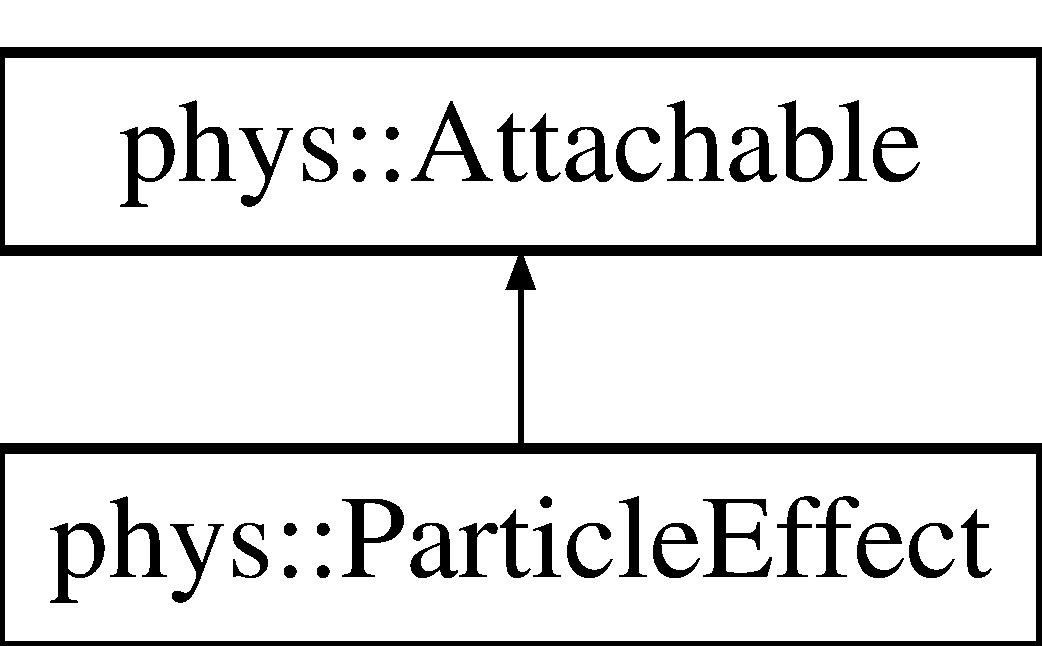
\includegraphics[height=2.000000cm]{d2/d69/classphys_1_1ParticleEffect}
\end{center}
\end{figure}
\subsubsection*{Public Member Functions}
\begin{DoxyCompactItemize}
\item 
\hyperlink{classphys_1_1ParticleEffect_a42d17b7cd81968603c70920c30e6f812}{ParticleEffect} (const \hyperlink{namespacephys_aa03900411993de7fbfec4789bc1d392e}{String} \&Name, const \hyperlink{namespacephys_aa03900411993de7fbfec4789bc1d392e}{String} \&Template, \hyperlink{classphys_1_1SceneManager}{SceneManager} $\ast$manager)
\begin{DoxyCompactList}\small\item\em Standard initialization constructor. \item\end{DoxyCompactList}\item 
\hyperlink{classphys_1_1ParticleEffect_a112c7e4b2ec7c34c3aba3bd422ef8a1c}{ParticleEffect} (Ogre::ParticleSystem $\ast$System, \hyperlink{classphys_1_1SceneManager}{SceneManager} $\ast$manager)
\begin{DoxyCompactList}\small\item\em Internal constructor. \item\end{DoxyCompactList}\item 
\hypertarget{classphys_1_1ParticleEffect_a8c9c3d0cd1d02acdc626266ee485f51f}{
\hyperlink{classphys_1_1ParticleEffect_a8c9c3d0cd1d02acdc626266ee485f51f}{$\sim$ParticleEffect} ()}
\label{d2/d69/classphys_1_1ParticleEffect_a8c9c3d0cd1d02acdc626266ee485f51f}

\begin{DoxyCompactList}\small\item\em Class destructor. \item\end{DoxyCompactList}\item 
\hyperlink{namespacephys_a5ce5049f8b4bf88d6413c47b504ebb31}{ConstString} \& \hyperlink{classphys_1_1ParticleEffect_a770309a3ec74b8bff6169ce5aecc64e7}{GetName} () const 
\begin{DoxyCompactList}\small\item\em Gets the name of this particle effect. \item\end{DoxyCompactList}\item 
void \hyperlink{classphys_1_1ParticleEffect_aee95ac9b688885361d3066a5a4b83965}{EnableParticleEffect} ()
\begin{DoxyCompactList}\small\item\em Enables the particle effect, allowing it to render. \item\end{DoxyCompactList}\item 
\hypertarget{classphys_1_1ParticleEffect_abd9f2339d22582055fe4ae45f986ff8c}{
void \hyperlink{classphys_1_1ParticleEffect_abd9f2339d22582055fe4ae45f986ff8c}{DisableParticleEffect} ()}
\label{d2/d69/classphys_1_1ParticleEffect_abd9f2339d22582055fe4ae45f986ff8c}

\begin{DoxyCompactList}\small\item\em Disables the particle effect, preventing it from rendering. \item\end{DoxyCompactList}\end{DoxyCompactItemize}
\subsubsection*{Friends}
\begin{DoxyCompactItemize}
\item 
\hypertarget{classphys_1_1ParticleEffect_a1cacd07efb11226da49a7c80569b18e8}{
class {\bfseries WorldNode}}
\label{d2/d69/classphys_1_1ParticleEffect_a1cacd07efb11226da49a7c80569b18e8}

\end{DoxyCompactItemize}


\subsubsection{Detailed Description}
This class is responsible for creating visual particle effects, such as rain, smoke, sparks, and explosions. Particle effects are loaded from particle scripts which are contained in particle files($\ast$.particle). \par
 All particle effects are created attached to a world node. The world Node provides the Nagivation functionality of for this 

Definition at line 68 of file particleeffect.h.



\subsubsection{Constructor \& Destructor Documentation}
\hypertarget{classphys_1_1ParticleEffect_a42d17b7cd81968603c70920c30e6f812}{
\index{phys::ParticleEffect@{phys::ParticleEffect}!ParticleEffect@{ParticleEffect}}
\index{ParticleEffect@{ParticleEffect}!phys::ParticleEffect@{phys::ParticleEffect}}
\paragraph[{ParticleEffect}]{\setlength{\rightskip}{0pt plus 5cm}phys::ParticleEffect::ParticleEffect (
\begin{DoxyParamCaption}
\item[{const {\bf String} \&}]{ Name, }
\item[{const {\bf String} \&}]{ Template, }
\item[{{\bf SceneManager} $\ast$}]{ manager}
\end{DoxyParamCaption}
)}\hfill}
\label{d2/d69/classphys_1_1ParticleEffect_a42d17b7cd81968603c70920c30e6f812}


Standard initialization constructor. 

Constructors 
\begin{DoxyParams}{Parameters}
\item[{\em Name}]The name of this particle effect. \item[{\em Template}]Name of the particle script to be used in creating this particle effect. \item[{\em manager}]Pointer to the manager that this particle effect is to be used in. \end{DoxyParams}


Definition at line 79 of file particleeffect.cpp.

\hypertarget{classphys_1_1ParticleEffect_a112c7e4b2ec7c34c3aba3bd422ef8a1c}{
\index{phys::ParticleEffect@{phys::ParticleEffect}!ParticleEffect@{ParticleEffect}}
\index{ParticleEffect@{ParticleEffect}!phys::ParticleEffect@{phys::ParticleEffect}}
\paragraph[{ParticleEffect}]{\setlength{\rightskip}{0pt plus 5cm}phys::ParticleEffect::ParticleEffect (
\begin{DoxyParamCaption}
\item[{Ogre::ParticleSystem $\ast$}]{ System, }
\item[{{\bf SceneManager} $\ast$}]{ manager}
\end{DoxyParamCaption}
)}\hfill}
\label{d2/d69/classphys_1_1ParticleEffect_a112c7e4b2ec7c34c3aba3bd422ef8a1c}


Internal constructor. 

This constructor should not be called on manually. 
\begin{DoxyParams}{Parameters}
\item[{\em System}]Pointer to the Ogre ParticleSystem this class is based on. \item[{\em manager}]Pointer to the manager that this particle effect is to be used in. \end{DoxyParams}


Definition at line 90 of file particleeffect.cpp.



\subsubsection{Member Function Documentation}
\hypertarget{classphys_1_1ParticleEffect_aee95ac9b688885361d3066a5a4b83965}{
\index{phys::ParticleEffect@{phys::ParticleEffect}!EnableParticleEffect@{EnableParticleEffect}}
\index{EnableParticleEffect@{EnableParticleEffect}!phys::ParticleEffect@{phys::ParticleEffect}}
\paragraph[{EnableParticleEffect}]{\setlength{\rightskip}{0pt plus 5cm}void phys::ParticleEffect::EnableParticleEffect (
\begin{DoxyParamCaption}
{}
\end{DoxyParamCaption}
)}\hfill}
\label{d2/d69/classphys_1_1ParticleEffect_aee95ac9b688885361d3066a5a4b83965}


Enables the particle effect, allowing it to render. 

Particle Functionality 

Definition at line 110 of file particleeffect.cpp.

\hypertarget{classphys_1_1ParticleEffect_a770309a3ec74b8bff6169ce5aecc64e7}{
\index{phys::ParticleEffect@{phys::ParticleEffect}!GetName@{GetName}}
\index{GetName@{GetName}!phys::ParticleEffect@{phys::ParticleEffect}}
\paragraph[{GetName}]{\setlength{\rightskip}{0pt plus 5cm}{\bf ConstString} \& phys::ParticleEffect::GetName (
\begin{DoxyParamCaption}
{}
\end{DoxyParamCaption}
) const\hspace{0.3cm}{\ttfamily  \mbox{[}virtual\mbox{]}}}\hfill}
\label{d2/d69/classphys_1_1ParticleEffect_a770309a3ec74b8bff6169ce5aecc64e7}


Gets the name of this particle effect. 

Inherited From \hyperlink{classphys_1_1Attachable}{Attachable} \begin{DoxyReturn}{Returns}
Returns a string containing the name given to this particle effect. 
\end{DoxyReturn}


Implements \hyperlink{classphys_1_1Attachable_a0a07d727fa2630dc3550fd991ca28256}{phys::Attachable}.



Definition at line 105 of file particleeffect.cpp.



The documentation for this class was generated from the following files:\begin{DoxyCompactItemize}
\item 
particleeffect.h\item 
particleeffect.cpp\end{DoxyCompactItemize}

\hypertarget{classphys_1_1PhysicsManager}{
\section{phys::PhysicsManager Class Reference}
\label{d3/dcc/classphys_1_1PhysicsManager}\index{phys::PhysicsManager@{phys::PhysicsManager}}
}


This is simply a place for storing all the Physics Related functions.  




{\ttfamily \#include $<$physicsmanager.h$>$}

Inheritance diagram for phys::PhysicsManager:\begin{figure}[H]
\begin{center}
\leavevmode
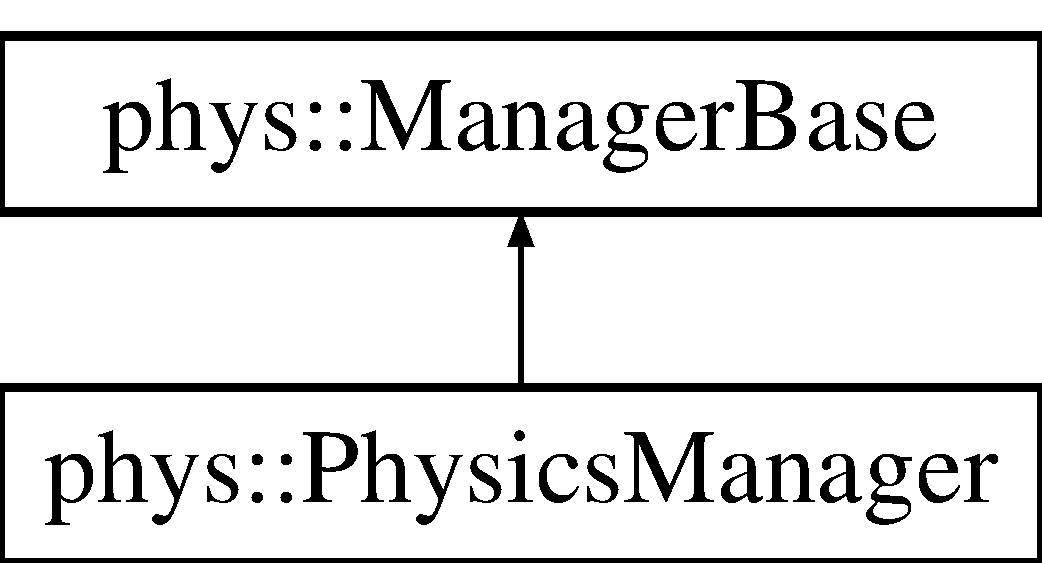
\includegraphics[height=2.000000cm]{d3/dcc/classphys_1_1PhysicsManager}
\end{center}
\end{figure}
\subsection*{Public Member Functions}
\begin{DoxyCompactItemize}
\item 
\hyperlink{classphys_1_1PhysicsManager_ab3ecdc295799ad9858ca80743b25006d}{PhysicsManager} ()
\begin{DoxyCompactList}\small\item\em Simple Constructor. \item\end{DoxyCompactList}\item 
\hyperlink{classphys_1_1PhysicsManager_a1072c647c64ec82381ddc9f1a17c5909}{PhysicsManager} (const \hyperlink{classphys_1_1Vector3}{Vector3} \&GeographyLowerBounds\_\-, const \hyperlink{classphys_1_1Vector3}{Vector3} \&GeographyUpperbounds\_\-, const unsigned short int \&MaxPhysicsProxies\_\-)
\begin{DoxyCompactList}\small\item\em Simple Constructor. \item\end{DoxyCompactList}\item 
virtual void \hyperlink{classphys_1_1PhysicsManager_a28885be750bb763d957f122593815388}{Initialize} ()
\begin{DoxyCompactList}\small\item\em This configures the Physics Manager to work with the Graphic settings. \item\end{DoxyCompactList}\item 
virtual void \hyperlink{classphys_1_1PhysicsManager_a62741a2582ac9bfd0255cf8a3ad2310c}{DoMainLoopItems} ()
\begin{DoxyCompactList}\small\item\em Physics stepping during the main loop. \item\end{DoxyCompactList}\item 
virtual \hyperlink{classphys_1_1PhysicsManager_a4898702f889c6b4aa7c0b59991d310b0}{$\sim$PhysicsManager} ()
\begin{DoxyCompactList}\small\item\em Deconstructor. \item\end{DoxyCompactList}\item 
void \hyperlink{classphys_1_1PhysicsManager_a3e74f3e0288706d44dc90657a8fa1118}{SetGravity} (\hyperlink{classphys_1_1Vector3}{Vector3} pgrav)
\begin{DoxyCompactList}\small\item\em Sets the gravity. \item\end{DoxyCompactList}\item 
\hyperlink{classphys_1_1Vector3}{Vector3} \hyperlink{classphys_1_1PhysicsManager_a880950ca6093afd3267dcadf30934574}{GetGravity} ()
\begin{DoxyCompactList}\small\item\em Gets the gravity. \item\end{DoxyCompactList}\item 
void \hyperlink{classphys_1_1PhysicsManager_acd1fe36f7cd593da0c466002304065eb}{SetSoftGravity} (\hyperlink{classphys_1_1Vector3}{Vector3} sgrav)
\begin{DoxyCompactList}\small\item\em Sets the gravity for soft bodies. \item\end{DoxyCompactList}\item 
\hyperlink{classphys_1_1Vector3}{Vector3} \hyperlink{classphys_1_1PhysicsManager_acdaad0849c3d6386e8cff5c98fc46664}{GetSoftGravity} ()
\begin{DoxyCompactList}\small\item\em Gets the soft body gravity. \item\end{DoxyCompactList}\item 
void \hyperlink{classphys_1_1PhysicsManager_af6acab3a35e52b1e25f1ab47f494d90d}{SetIndividualGravity} (\hyperlink{classphys_1_1ActorBase}{ActorBase} $\ast$Actor, \hyperlink{classphys_1_1Vector3}{Vector3} igrav)
\begin{DoxyCompactList}\small\item\em Sets the gravity to be applied to a single object. \item\end{DoxyCompactList}\item 
void \hyperlink{classphys_1_1PhysicsManager_a67fb59148a94ced0a92b288a638f89db}{SetDebugPhysicsRendering} (int ToBeEnabled)
\begin{DoxyCompactList}\small\item\em Enables and Disables Physics Debug Drawing. \item\end{DoxyCompactList}\item 
int \hyperlink{classphys_1_1PhysicsManager_a64f96d2e4b25c2b9a66042998bf334ff}{GetDebugPhysicsRendering} ()
\begin{DoxyCompactList}\small\item\em Is Physics Debug Drawing currently enabled? \item\end{DoxyCompactList}\item 
void \hyperlink{classphys_1_1PhysicsManager_ab43a963cf26ca4293a7c34a2a68c4f2c}{SetDebugPhysicsWireCount} (\hyperlink{namespacephys_a460f6bc24c8dd347b05e0366ae34f34a}{Whole} WireFrameCount\_\-)
\begin{DoxyCompactList}\small\item\em How many Wireframes do you want drawn from previous events. \item\end{DoxyCompactList}\item 
\hyperlink{namespacephys_a460f6bc24c8dd347b05e0366ae34f34a}{Whole} \hyperlink{classphys_1_1PhysicsManager_a8f46e55e4cadfcd1c2c03bcdbfe6c06f}{GetDebugPhysicsWireCount} ()
\begin{DoxyCompactList}\small\item\em This gets how many WireFrames are being drawn. \item\end{DoxyCompactList}\item 
void \hyperlink{classphys_1_1PhysicsManager_ad363d6683a0276395eeb2c42a56f95fc}{DoMainLoopItems} (const \hyperlink{namespacephys_af7eb897198d265b8e868f45240230d5f}{Real} \&TimeElapsed)
\begin{DoxyCompactList}\small\item\em This does all the work reuired for the main loop to process physics. \item\end{DoxyCompactList}\item 
\hyperlink{classphys_1_1Vector3}{Vector3} \hyperlink{classphys_1_1PhysicsManager_a54a48fdfd9db914c25a0f892c2f56301}{GetActorOffset} (const \hyperlink{classphys_1_1Vector3WActor}{Vector3WActor} \&OffsetInfo)
\begin{DoxyCompactList}\small\item\em Gets the offset between a point and an actor. \item\end{DoxyCompactList}\item 
void \hyperlink{classphys_1_1PhysicsManager_ab31bf38e9ed68c484946731546425691}{AddConstraint} (\hyperlink{classphys_1_1TypedConstraint}{TypedConstraint} $\ast$Constraint)
\begin{DoxyCompactList}\small\item\em Adds a constraint to the world. \item\end{DoxyCompactList}\item 
void \hyperlink{classphys_1_1PhysicsManager_ace94aa20b5191b01630e7a5046cb7af6}{RemoveConstraint} (\hyperlink{classphys_1_1TypedConstraint}{TypedConstraint} $\ast$Constraint)
\begin{DoxyCompactList}\small\item\em Removes a constraint from the world. \item\end{DoxyCompactList}\item 
void \hyperlink{classphys_1_1PhysicsManager_a24fae734b5750db6fc1d2b1e3656bb71}{StorePhysicsShape} (\hyperlink{classphys_1_1ActorBase}{ActorBase} $\ast$Actor, \hyperlink{namespacephys_aa03900411993de7fbfec4789bc1d392e}{String} \&ShapeName)
\begin{DoxyCompactList}\small\item\em Stores an already generated physics shape. \item\end{DoxyCompactList}\item 
void \hyperlink{classphys_1_1PhysicsManager_a58653c59133900a432169a7c980105ce}{ApplyPhysicsShape} (\hyperlink{classphys_1_1ActorBase}{ActorBase} $\ast$Actor, \hyperlink{namespacephys_aa03900411993de7fbfec4789bc1d392e}{String} \&ShapeName)
\begin{DoxyCompactList}\small\item\em Applies a previously stored shape. \item\end{DoxyCompactList}\item 
void \hyperlink{classphys_1_1PhysicsManager_a64e75a71598b6440c4feb1a2214a1420}{AddAreaEffect} (\hyperlink{classphys_1_1AreaEffect}{AreaEffect} $\ast$AE)
\begin{DoxyCompactList}\small\item\em Adds an area effect to the world. \item\end{DoxyCompactList}\item 
void \hyperlink{classphys_1_1PhysicsManager_a5ee0f784a8239be56164a7a67a28f227}{RemoveAreaEffect} (\hyperlink{classphys_1_1AreaEffect}{AreaEffect} $\ast$AE)
\begin{DoxyCompactList}\small\item\em Removes an area effect from the world. \item\end{DoxyCompactList}\item 
\hyperlink{classphys_1_1AreaEffect}{AreaEffect} $\ast$ \hyperlink{classphys_1_1PhysicsManager_a36b575504b1de592ee24d08ebf1fd620}{GetAreaEffect} (\hyperlink{namespacephys_aa03900411993de7fbfec4789bc1d392e}{String} Name)
\begin{DoxyCompactList}\small\item\em Gets an Area Effect by name. \item\end{DoxyCompactList}\item 
void \hyperlink{classphys_1_1PhysicsManager_a98ee9704eec230ff759850ffa8394489}{SetCollisionParams} (const unsigned short int Age, \hyperlink{namespacephys_af7eb897198d265b8e868f45240230d5f}{Real} Force)
\begin{DoxyCompactList}\small\item\em Sets the Collision Parameters. \item\end{DoxyCompactList}\item 
unsigned short int \hyperlink{classphys_1_1PhysicsManager_a4232e8cd52e70b623ef30c40be6cdb4a}{GetCollisionAge} ()
\begin{DoxyCompactList}\small\item\em Gets the Collision Age limit. \item\end{DoxyCompactList}\item 
\hyperlink{namespacephys_af7eb897198d265b8e868f45240230d5f}{Real} \hyperlink{classphys_1_1PhysicsManager_ad11ee3904e1725f95ce9bd58f4ee3925}{GetImpulse} ()
\begin{DoxyCompactList}\small\item\em Gets the Collision Impulse limit. \item\end{DoxyCompactList}\item 
btSoftRigidDynamicsWorld $\ast$ \hyperlink{classphys_1_1PhysicsManager_a4b4f8a23259a94a50c81649f39256d7f}{GetPhysicsWorldPointer} ()
\begin{DoxyCompactList}\small\item\em This returns a pointer to the bullet physics world. This is for internal use only. \item\end{DoxyCompactList}\item 
virtual \hyperlink{classphys_1_1ManagerBase_aaa6ccddf23892eaccb898529414f80a5}{ManagerTypeName} \hyperlink{classphys_1_1PhysicsManager_a4d151cd24052ef3cccde6b66b8745be6}{GetType} () const 
\begin{DoxyCompactList}\small\item\em This returns the type of this manager. \item\end{DoxyCompactList}\end{DoxyCompactItemize}


\subsection{Detailed Description}
This is simply a place for storing all the Physics Related functions. This is a place for storing items related to Debug physics drawing, Adding constraints, screwing with gravity and doing other physics Related features. 

Definition at line 79 of file physicsmanager.h.



\subsection{Constructor \& Destructor Documentation}
\hypertarget{classphys_1_1PhysicsManager_ab3ecdc295799ad9858ca80743b25006d}{
\index{phys::PhysicsManager@{phys::PhysicsManager}!PhysicsManager@{PhysicsManager}}
\index{PhysicsManager@{PhysicsManager}!phys::PhysicsManager@{phys::PhysicsManager}}
\subsubsection[{PhysicsManager}]{\setlength{\rightskip}{0pt plus 5cm}phys::PhysicsManager::PhysicsManager (
\begin{DoxyParamCaption}
{}
\end{DoxyParamCaption}
)}}
\label{d3/dcc/classphys_1_1PhysicsManager_ab3ecdc295799ad9858ca80743b25006d}


Simple Constructor. 

This constructor will assign some sane default values and will create a physics world that can be used immediately 

Definition at line 263 of file physicsmanager.cpp.

\hypertarget{classphys_1_1PhysicsManager_a1072c647c64ec82381ddc9f1a17c5909}{
\index{phys::PhysicsManager@{phys::PhysicsManager}!PhysicsManager@{PhysicsManager}}
\index{PhysicsManager@{PhysicsManager}!phys::PhysicsManager@{phys::PhysicsManager}}
\subsubsection[{PhysicsManager}]{\setlength{\rightskip}{0pt plus 5cm}phys::PhysicsManager::PhysicsManager (
\begin{DoxyParamCaption}
\item[{const {\bf Vector3} \&}]{ GeographyLowerBounds\_\-, }
\item[{const {\bf Vector3} \&}]{ GeographyUpperbounds\_\-, }
\item[{const unsigned short int \&}]{ MaxPhysicsProxies\_\-}
\end{DoxyParamCaption}
)}}
\label{d3/dcc/classphys_1_1PhysicsManager_a1072c647c64ec82381ddc9f1a17c5909}


Simple Constructor. 

This constructor will assign some sane default values and will create a physics world that can be used immediately 
\begin{DoxyParams}{Parameters}
\item[{\em GeographyLowerBounds\_\-}]This \hyperlink{classphys_1_1Vector3}{Vector3} will loosely represent the lower right conrer of the world \item[{\em GeographyUpperbounds\_\-}]This \hyperlink{classphys_1_1Vector3}{Vector3} will loosely represent the upper left conrer of the world \item[{\em MaxPhysicsProxies\_\-}]This approximates the maximum amount of items allowed in the physics world \end{DoxyParams}


Definition at line 268 of file physicsmanager.cpp.

\hypertarget{classphys_1_1PhysicsManager_a4898702f889c6b4aa7c0b59991d310b0}{
\index{phys::PhysicsManager@{phys::PhysicsManager}!$\sim$PhysicsManager@{$\sim$PhysicsManager}}
\index{$\sim$PhysicsManager@{$\sim$PhysicsManager}!phys::PhysicsManager@{phys::PhysicsManager}}
\subsubsection[{$\sim$PhysicsManager}]{\setlength{\rightskip}{0pt plus 5cm}phys::PhysicsManager::$\sim$PhysicsManager (
\begin{DoxyParamCaption}
{}
\end{DoxyParamCaption}
)\hspace{0.3cm}{\ttfamily  \mbox{[}virtual\mbox{]}}}}
\label{d3/dcc/classphys_1_1PhysicsManager_a4898702f889c6b4aa7c0b59991d310b0}


Deconstructor. 

This deletes all those crazy pointers that Bullet, the physics subsystem need. 

Definition at line 273 of file physicsmanager.cpp.



\subsection{Member Function Documentation}
\hypertarget{classphys_1_1PhysicsManager_a64e75a71598b6440c4feb1a2214a1420}{
\index{phys::PhysicsManager@{phys::PhysicsManager}!AddAreaEffect@{AddAreaEffect}}
\index{AddAreaEffect@{AddAreaEffect}!phys::PhysicsManager@{phys::PhysicsManager}}
\subsubsection[{AddAreaEffect}]{\setlength{\rightskip}{0pt plus 5cm}void phys::PhysicsManager::AddAreaEffect (
\begin{DoxyParamCaption}
\item[{{\bf AreaEffect} $\ast$}]{ AE}
\end{DoxyParamCaption}
)}}
\label{d3/dcc/classphys_1_1PhysicsManager_a64e75a71598b6440c4feb1a2214a1420}


Adds an area effect to the world. 

Adds an area effect to the world so that it can/will take effect. 
\begin{DoxyParams}{Parameters}
\item[{\em AE}]The area effect to be added. \end{DoxyParams}


Definition at line 496 of file physicsmanager.cpp.

\hypertarget{classphys_1_1PhysicsManager_ab31bf38e9ed68c484946731546425691}{
\index{phys::PhysicsManager@{phys::PhysicsManager}!AddConstraint@{AddConstraint}}
\index{AddConstraint@{AddConstraint}!phys::PhysicsManager@{phys::PhysicsManager}}
\subsubsection[{AddConstraint}]{\setlength{\rightskip}{0pt plus 5cm}void phys::PhysicsManager::AddConstraint (
\begin{DoxyParamCaption}
\item[{{\bf TypedConstraint} $\ast$}]{ Constraint}
\end{DoxyParamCaption}
)}}
\label{d3/dcc/classphys_1_1PhysicsManager_ab31bf38e9ed68c484946731546425691}


Adds a constraint to the world. 

Adds the constraint to the world so that it can/will take effect. 
\begin{DoxyParams}{Parameters}
\item[{\em Constraint}]The constraint to be added. \end{DoxyParams}


Definition at line 486 of file physicsmanager.cpp.

\hypertarget{classphys_1_1PhysicsManager_a58653c59133900a432169a7c980105ce}{
\index{phys::PhysicsManager@{phys::PhysicsManager}!ApplyPhysicsShape@{ApplyPhysicsShape}}
\index{ApplyPhysicsShape@{ApplyPhysicsShape}!phys::PhysicsManager@{phys::PhysicsManager}}
\subsubsection[{ApplyPhysicsShape}]{\setlength{\rightskip}{0pt plus 5cm}void phys::PhysicsManager::ApplyPhysicsShape (
\begin{DoxyParamCaption}
\item[{{\bf ActorBase} $\ast$}]{ Actor, }
\item[{{\bf String} \&}]{ ShapeName}
\end{DoxyParamCaption}
)}}
\label{d3/dcc/classphys_1_1PhysicsManager_a58653c59133900a432169a7c980105ce}


Applies a previously stored shape. 

This function will take a stored shape and apply it to the actor provided. 
\begin{DoxyParams}{Parameters}
\item[{\em Actor}]The actor to which you want to apply the shape. \item[{\em ShapeName}]The name of the shape you wish to have applied to the actor. \end{DoxyParams}


Definition at line 544 of file physicsmanager.cpp.

\hypertarget{classphys_1_1PhysicsManager_a62741a2582ac9bfd0255cf8a3ad2310c}{
\index{phys::PhysicsManager@{phys::PhysicsManager}!DoMainLoopItems@{DoMainLoopItems}}
\index{DoMainLoopItems@{DoMainLoopItems}!phys::PhysicsManager@{phys::PhysicsManager}}
\subsubsection[{DoMainLoopItems}]{\setlength{\rightskip}{0pt plus 5cm}void phys::PhysicsManager::DoMainLoopItems (
\begin{DoxyParamCaption}
{}
\end{DoxyParamCaption}
)\hspace{0.3cm}{\ttfamily  \mbox{[}virtual\mbox{]}}}}
\label{d3/dcc/classphys_1_1PhysicsManager_a62741a2582ac9bfd0255cf8a3ad2310c}


Physics stepping during the main loop. 

This increments the the physics world the required amount to keep it in sync with the Graphics/Timing. 

Implements \hyperlink{classphys_1_1ManagerBase_aa9e13a3f7c398b708f0f242610b5abf7}{phys::ManagerBase}.



Definition at line 345 of file physicsmanager.cpp.

\hypertarget{classphys_1_1PhysicsManager_ad363d6683a0276395eeb2c42a56f95fc}{
\index{phys::PhysicsManager@{phys::PhysicsManager}!DoMainLoopItems@{DoMainLoopItems}}
\index{DoMainLoopItems@{DoMainLoopItems}!phys::PhysicsManager@{phys::PhysicsManager}}
\subsubsection[{DoMainLoopItems}]{\setlength{\rightskip}{0pt plus 5cm}void phys::PhysicsManager::DoMainLoopItems (
\begin{DoxyParamCaption}
\item[{const {\bf Real} \&}]{ TimeElapsed}
\end{DoxyParamCaption}
)}}
\label{d3/dcc/classphys_1_1PhysicsManager_ad363d6683a0276395eeb2c42a56f95fc}


This does all the work reuired for the main loop to process physics. 


\begin{DoxyParams}{Parameters}
\item[{\em TimeElapsed}]This is a real that represents the amount of time we need to simulate \end{DoxyParams}


Definition at line 350 of file physicsmanager.cpp.

\hypertarget{classphys_1_1PhysicsManager_a54a48fdfd9db914c25a0f892c2f56301}{
\index{phys::PhysicsManager@{phys::PhysicsManager}!GetActorOffset@{GetActorOffset}}
\index{GetActorOffset@{GetActorOffset}!phys::PhysicsManager@{phys::PhysicsManager}}
\subsubsection[{GetActorOffset}]{\setlength{\rightskip}{0pt plus 5cm}{\bf Vector3} phys::PhysicsManager::GetActorOffset (
\begin{DoxyParamCaption}
\item[{const {\bf Vector3WActor} \&}]{ OffsetInfo}
\end{DoxyParamCaption}
)}}
\label{d3/dcc/classphys_1_1PhysicsManager_a54a48fdfd9db914c25a0f892c2f56301}


Gets the offset between a point and an actor. 

This function will return the offset between the specified world point and the specified actors center of mass. 
\begin{DoxyParams}{Parameters}
\item[{\em OffsetInfo}]The vector and actor to compare for offset data. \end{DoxyParams}
\begin{DoxyReturn}{Returns}
Returns the \hyperlink{classphys_1_1Vector3}{Vector3} representing the actors offset from the world point. 
\end{DoxyReturn}


Definition at line 473 of file physicsmanager.cpp.

\hypertarget{classphys_1_1PhysicsManager_a36b575504b1de592ee24d08ebf1fd620}{
\index{phys::PhysicsManager@{phys::PhysicsManager}!GetAreaEffect@{GetAreaEffect}}
\index{GetAreaEffect@{GetAreaEffect}!phys::PhysicsManager@{phys::PhysicsManager}}
\subsubsection[{GetAreaEffect}]{\setlength{\rightskip}{0pt plus 5cm}{\bf AreaEffect} $\ast$ phys::PhysicsManager::GetAreaEffect (
\begin{DoxyParamCaption}
\item[{{\bf String}}]{ Name}
\end{DoxyParamCaption}
)}}
\label{d3/dcc/classphys_1_1PhysicsManager_a36b575504b1de592ee24d08ebf1fd620}


Gets an Area Effect by name. 

This function will return the named area effect if it is stored. 
\begin{DoxyParams}{Parameters}
\item[{\em Name}]The name of the area effect to find. \end{DoxyParams}
\begin{DoxyReturn}{Returns}
Returns a pointer to the named area effect. 
\end{DoxyReturn}


Definition at line 514 of file physicsmanager.cpp.

\hypertarget{classphys_1_1PhysicsManager_a4232e8cd52e70b623ef30c40be6cdb4a}{
\index{phys::PhysicsManager@{phys::PhysicsManager}!GetCollisionAge@{GetCollisionAge}}
\index{GetCollisionAge@{GetCollisionAge}!phys::PhysicsManager@{phys::PhysicsManager}}
\subsubsection[{GetCollisionAge}]{\setlength{\rightskip}{0pt plus 5cm}unsigned short int phys::PhysicsManager::GetCollisionAge (
\begin{DoxyParamCaption}
{}
\end{DoxyParamCaption}
)}}
\label{d3/dcc/classphys_1_1PhysicsManager_a4232e8cd52e70b623ef30c40be6cdb4a}


Gets the Collision Age limit. 

Gets the CollisionAge used in filtering out collision contacts used to make events. \begin{DoxyReturn}{Returns}
This function will return the number of physics ticks the collision has to have existed to be used. 
\end{DoxyReturn}


Definition at line 556 of file physicsmanager.cpp.

\hypertarget{classphys_1_1PhysicsManager_a64f96d2e4b25c2b9a66042998bf334ff}{
\index{phys::PhysicsManager@{phys::PhysicsManager}!GetDebugPhysicsRendering@{GetDebugPhysicsRendering}}
\index{GetDebugPhysicsRendering@{GetDebugPhysicsRendering}!phys::PhysicsManager@{phys::PhysicsManager}}
\subsubsection[{GetDebugPhysicsRendering}]{\setlength{\rightskip}{0pt plus 5cm}int phys::PhysicsManager::GetDebugPhysicsRendering (
\begin{DoxyParamCaption}
{}
\end{DoxyParamCaption}
)}}
\label{d3/dcc/classphys_1_1PhysicsManager_a64f96d2e4b25c2b9a66042998bf334ff}


Is Physics Debug Drawing currently enabled? 

lets you check if Physics Debug Drawing is enabled or not. \begin{DoxyReturn}{Returns}
1 for it is on, and 0 for it is not. The may be other options later for selectively cnacking certain features 
\end{DoxyReturn}


Definition at line 448 of file physicsmanager.cpp.

\hypertarget{classphys_1_1PhysicsManager_a8f46e55e4cadfcd1c2c03bcdbfe6c06f}{
\index{phys::PhysicsManager@{phys::PhysicsManager}!GetDebugPhysicsWireCount@{GetDebugPhysicsWireCount}}
\index{GetDebugPhysicsWireCount@{GetDebugPhysicsWireCount}!phys::PhysicsManager@{phys::PhysicsManager}}
\subsubsection[{GetDebugPhysicsWireCount}]{\setlength{\rightskip}{0pt plus 5cm}{\bf Whole} phys::PhysicsManager::GetDebugPhysicsWireCount (
\begin{DoxyParamCaption}
{}
\end{DoxyParamCaption}
)}}
\label{d3/dcc/classphys_1_1PhysicsManager_a8f46e55e4cadfcd1c2c03bcdbfe6c06f}


This gets how many WireFrames are being drawn. 

This will tell you how many frames worth of previous in game events are being drawn. \begin{DoxyReturn}{Returns}
This returns either 2 or the last amount passed into World::SetDebugPhysicsWireCount . 
\end{DoxyReturn}


Definition at line 463 of file physicsmanager.cpp.

\hypertarget{classphys_1_1PhysicsManager_a880950ca6093afd3267dcadf30934574}{
\index{phys::PhysicsManager@{phys::PhysicsManager}!GetGravity@{GetGravity}}
\index{GetGravity@{GetGravity}!phys::PhysicsManager@{phys::PhysicsManager}}
\subsubsection[{GetGravity}]{\setlength{\rightskip}{0pt plus 5cm}{\bf Vector3} phys::PhysicsManager::GetGravity (
\begin{DoxyParamCaption}
{}
\end{DoxyParamCaption}
)}}
\label{d3/dcc/classphys_1_1PhysicsManager_a880950ca6093afd3267dcadf30934574}


Gets the gravity. 

Gets the currently set world gravity. \begin{DoxyReturn}{Returns}
Returns the currently set world gravity. 
\end{DoxyReturn}


Definition at line 409 of file physicsmanager.cpp.

\hypertarget{classphys_1_1PhysicsManager_ad11ee3904e1725f95ce9bd58f4ee3925}{
\index{phys::PhysicsManager@{phys::PhysicsManager}!GetImpulse@{GetImpulse}}
\index{GetImpulse@{GetImpulse}!phys::PhysicsManager@{phys::PhysicsManager}}
\subsubsection[{GetImpulse}]{\setlength{\rightskip}{0pt plus 5cm}{\bf Real} phys::PhysicsManager::GetImpulse (
\begin{DoxyParamCaption}
{}
\end{DoxyParamCaption}
)}}
\label{d3/dcc/classphys_1_1PhysicsManager_ad11ee3904e1725f95ce9bd58f4ee3925}


Gets the Collision Impulse limit. 

Gets the Collision Impulse used in filtering out collision contacts used to make events. \begin{DoxyReturn}{Returns}
This function will return the lower limit of the allowed force of the collision to generate an event. 
\end{DoxyReturn}


Definition at line 561 of file physicsmanager.cpp.

\hypertarget{classphys_1_1PhysicsManager_a4b4f8a23259a94a50c81649f39256d7f}{
\index{phys::PhysicsManager@{phys::PhysicsManager}!GetPhysicsWorldPointer@{GetPhysicsWorldPointer}}
\index{GetPhysicsWorldPointer@{GetPhysicsWorldPointer}!phys::PhysicsManager@{phys::PhysicsManager}}
\subsubsection[{GetPhysicsWorldPointer}]{\setlength{\rightskip}{0pt plus 5cm}btSoftRigidDynamicsWorld $\ast$ phys::PhysicsManager::GetPhysicsWorldPointer (
\begin{DoxyParamCaption}
{}
\end{DoxyParamCaption}
)}}
\label{d3/dcc/classphys_1_1PhysicsManager_a4b4f8a23259a94a50c81649f39256d7f}


This returns a pointer to the bullet physics world. This is for internal use only. 

\begin{DoxyInternal}{For internal use only.}
\end{DoxyInternal}


Definition at line 468 of file physicsmanager.cpp.

\hypertarget{classphys_1_1PhysicsManager_acdaad0849c3d6386e8cff5c98fc46664}{
\index{phys::PhysicsManager@{phys::PhysicsManager}!GetSoftGravity@{GetSoftGravity}}
\index{GetSoftGravity@{GetSoftGravity}!phys::PhysicsManager@{phys::PhysicsManager}}
\subsubsection[{GetSoftGravity}]{\setlength{\rightskip}{0pt plus 5cm}{\bf Vector3} phys::PhysicsManager::GetSoftGravity (
\begin{DoxyParamCaption}
{}
\end{DoxyParamCaption}
)}}
\label{d3/dcc/classphys_1_1PhysicsManager_acdaad0849c3d6386e8cff5c98fc46664}


Gets the soft body gravity. 

Gets the currently set soft body world gravity. \begin{DoxyReturn}{Returns}
Returns the currently set soft body world gravity. 
\end{DoxyReturn}


Definition at line 420 of file physicsmanager.cpp.

\hypertarget{classphys_1_1PhysicsManager_a4d151cd24052ef3cccde6b66b8745be6}{
\index{phys::PhysicsManager@{phys::PhysicsManager}!GetType@{GetType}}
\index{GetType@{GetType}!phys::PhysicsManager@{phys::PhysicsManager}}
\subsubsection[{GetType}]{\setlength{\rightskip}{0pt plus 5cm}{\bf ManagerBase::ManagerTypeName} phys::PhysicsManager::GetType (
\begin{DoxyParamCaption}
{}
\end{DoxyParamCaption}
) const\hspace{0.3cm}{\ttfamily  \mbox{[}virtual\mbox{]}}}}
\label{d3/dcc/classphys_1_1PhysicsManager_a4d151cd24052ef3cccde6b66b8745be6}


This returns the type of this manager. 

\begin{DoxyReturn}{Returns}
This returns ManagerTypeName::PhysicsManager 
\end{DoxyReturn}


Implements \hyperlink{classphys_1_1ManagerBase_aff400b6599db635e24796d8221e9a0e3}{phys::ManagerBase}.



Definition at line 567 of file physicsmanager.cpp.

\hypertarget{classphys_1_1PhysicsManager_a28885be750bb763d957f122593815388}{
\index{phys::PhysicsManager@{phys::PhysicsManager}!Initialize@{Initialize}}
\index{Initialize@{Initialize}!phys::PhysicsManager@{phys::PhysicsManager}}
\subsubsection[{Initialize}]{\setlength{\rightskip}{0pt plus 5cm}void phys::PhysicsManager::Initialize (
\begin{DoxyParamCaption}
{}
\end{DoxyParamCaption}
)\hspace{0.3cm}{\ttfamily  \mbox{[}virtual\mbox{]}}}}
\label{d3/dcc/classphys_1_1PhysicsManager_a28885be750bb763d957f122593815388}


This configures the Physics Manager to work with the Graphic settings. 

This configures the Physics manager to work with the existing graphics settings. This must be called before the physics manager is used, but after the graphics have been initialized 

\begin{Desc}
\item[\hyperlink{todo__todo000022}{Todo}]Possibly restructure this so that it'll detect ogre first, preventing a crash. At current this makes the physics manager depend on the graphicsmanager. \end{Desc}




Implements \hyperlink{classphys_1_1ManagerBase_a57dd8e54e767427d5bdcc86dc66d73ed}{phys::ManagerBase}.



Definition at line 336 of file physicsmanager.cpp.

\hypertarget{classphys_1_1PhysicsManager_a5ee0f784a8239be56164a7a67a28f227}{
\index{phys::PhysicsManager@{phys::PhysicsManager}!RemoveAreaEffect@{RemoveAreaEffect}}
\index{RemoveAreaEffect@{RemoveAreaEffect}!phys::PhysicsManager@{phys::PhysicsManager}}
\subsubsection[{RemoveAreaEffect}]{\setlength{\rightskip}{0pt plus 5cm}void phys::PhysicsManager::RemoveAreaEffect (
\begin{DoxyParamCaption}
\item[{{\bf AreaEffect} $\ast$}]{ AE}
\end{DoxyParamCaption}
)}}
\label{d3/dcc/classphys_1_1PhysicsManager_a5ee0f784a8239be56164a7a67a28f227}


Removes an area effect from the world. 

Removes an area effect from the world so that it will have no effect. 
\begin{DoxyParams}{Parameters}
\item[{\em AE}]The area effect to be removed. \end{DoxyParams}


Definition at line 502 of file physicsmanager.cpp.

\hypertarget{classphys_1_1PhysicsManager_ace94aa20b5191b01630e7a5046cb7af6}{
\index{phys::PhysicsManager@{phys::PhysicsManager}!RemoveConstraint@{RemoveConstraint}}
\index{RemoveConstraint@{RemoveConstraint}!phys::PhysicsManager@{phys::PhysicsManager}}
\subsubsection[{RemoveConstraint}]{\setlength{\rightskip}{0pt plus 5cm}void phys::PhysicsManager::RemoveConstraint (
\begin{DoxyParamCaption}
\item[{{\bf TypedConstraint} $\ast$}]{ Constraint}
\end{DoxyParamCaption}
)}}
\label{d3/dcc/classphys_1_1PhysicsManager_ace94aa20b5191b01630e7a5046cb7af6}


Removes a constraint from the world. 

Removes a constraint from the world so that it will have no effect. 
\begin{DoxyParams}{Parameters}
\item[{\em Constraint}]The constraint to be removed. \end{DoxyParams}


Definition at line 491 of file physicsmanager.cpp.

\hypertarget{classphys_1_1PhysicsManager_a98ee9704eec230ff759850ffa8394489}{
\index{phys::PhysicsManager@{phys::PhysicsManager}!SetCollisionParams@{SetCollisionParams}}
\index{SetCollisionParams@{SetCollisionParams}!phys::PhysicsManager@{phys::PhysicsManager}}
\subsubsection[{SetCollisionParams}]{\setlength{\rightskip}{0pt plus 5cm}void phys::PhysicsManager::SetCollisionParams (
\begin{DoxyParamCaption}
\item[{const unsigned short int}]{ Age, }
\item[{{\bf Real}}]{ Force}
\end{DoxyParamCaption}
)}}
\label{d3/dcc/classphys_1_1PhysicsManager_a98ee9704eec230ff759850ffa8394489}


Sets the Collision Parameters. 

Sets the Collision Age and Force Filters used in filtering out collision contacts used to make events. The lower these numbers, the more events will be generated. \par
 These numbers both default to 1. 
\begin{DoxyParams}{Parameters}
\item[{\em Age}]The number of physics ticks the collision has to have existed to be used. Usually you want 1 or 2. Default: 1 \item[{\em Force}]The amount of force applied in the collision to filter by. This amount can vary more then the other param based on what you need. Default: 1.0 \end{DoxyParams}


Definition at line 550 of file physicsmanager.cpp.

\hypertarget{classphys_1_1PhysicsManager_a67fb59148a94ced0a92b288a638f89db}{
\index{phys::PhysicsManager@{phys::PhysicsManager}!SetDebugPhysicsRendering@{SetDebugPhysicsRendering}}
\index{SetDebugPhysicsRendering@{SetDebugPhysicsRendering}!phys::PhysicsManager@{phys::PhysicsManager}}
\subsubsection[{SetDebugPhysicsRendering}]{\setlength{\rightskip}{0pt plus 5cm}void phys::PhysicsManager::SetDebugPhysicsRendering (
\begin{DoxyParamCaption}
\item[{int}]{ ToBeEnabled}
\end{DoxyParamCaption}
)}}
\label{d3/dcc/classphys_1_1PhysicsManager_a67fb59148a94ced0a92b288a638f89db}


Enables and Disables Physics Debug Drawing. 

Enables and Disables Physics Debug Drawing using default wireframes. This will force renderings that match the physics subsytem pixel for pixel. 
\begin{DoxyParams}{Parameters}
\item[{\em ToBeEnabled}]1 to turn it on, 0 to turn it off. There may be other options in the future, to enable fine tuned control \end{DoxyParams}


Definition at line 438 of file physicsmanager.cpp.

\hypertarget{classphys_1_1PhysicsManager_ab43a963cf26ca4293a7c34a2a68c4f2c}{
\index{phys::PhysicsManager@{phys::PhysicsManager}!SetDebugPhysicsWireCount@{SetDebugPhysicsWireCount}}
\index{SetDebugPhysicsWireCount@{SetDebugPhysicsWireCount}!phys::PhysicsManager@{phys::PhysicsManager}}
\subsubsection[{SetDebugPhysicsWireCount}]{\setlength{\rightskip}{0pt plus 5cm}void phys::PhysicsManager::SetDebugPhysicsWireCount (
\begin{DoxyParamCaption}
\item[{{\bf Whole}}]{ WireFrameCount\_\-}
\end{DoxyParamCaption}
)}}
\label{d3/dcc/classphys_1_1PhysicsManager_ab43a963cf26ca4293a7c34a2a68c4f2c}


How many Wireframes do you want drawn from previous events. 

Each frame of the action gets its own wire frame, and how many of those back did you want to see? To see a minimal amount set this to 2, as the first wireframe is commonly entirely inside the the rendered 3d mesh. You can use \hyperlink{classphys_1_1World_aa063ace52be484c7b03ec5859453f48b}{World::GetTargetFrameTime()} In conjunction with this to specify an amout of seconds worth of wireframes. 
\begin{DoxyParams}{Parameters}
\item[{\em WireFrameCount\_\-}]This is a whole number that is the amount of wire frames you wan to see. Don't forget to be mindful of the framerate, Any amount more than just a few seconds worth can be cumbersome. \end{DoxyParams}


Definition at line 458 of file physicsmanager.cpp.

\hypertarget{classphys_1_1PhysicsManager_a3e74f3e0288706d44dc90657a8fa1118}{
\index{phys::PhysicsManager@{phys::PhysicsManager}!SetGravity@{SetGravity}}
\index{SetGravity@{SetGravity}!phys::PhysicsManager@{phys::PhysicsManager}}
\subsubsection[{SetGravity}]{\setlength{\rightskip}{0pt plus 5cm}void phys::PhysicsManager::SetGravity (
\begin{DoxyParamCaption}
\item[{{\bf Vector3}}]{ pgrav}
\end{DoxyParamCaption}
)}}
\label{d3/dcc/classphys_1_1PhysicsManager_a3e74f3e0288706d44dc90657a8fa1118}


Sets the gravity. 

Sets the strength and direction of gravity within the world. 
\begin{DoxyParams}{Parameters}
\item[{\em pgrav}]\hyperlink{classphys_1_1Vector3}{Vector3} representing the strength and direction of gravity. \end{DoxyParams}


Definition at line 404 of file physicsmanager.cpp.

\hypertarget{classphys_1_1PhysicsManager_af6acab3a35e52b1e25f1ab47f494d90d}{
\index{phys::PhysicsManager@{phys::PhysicsManager}!SetIndividualGravity@{SetIndividualGravity}}
\index{SetIndividualGravity@{SetIndividualGravity}!phys::PhysicsManager@{phys::PhysicsManager}}
\subsubsection[{SetIndividualGravity}]{\setlength{\rightskip}{0pt plus 5cm}void phys::PhysicsManager::SetIndividualGravity (
\begin{DoxyParamCaption}
\item[{{\bf ActorBase} $\ast$}]{ Actor, }
\item[{{\bf Vector3}}]{ igrav}
\end{DoxyParamCaption}
)}}
\label{d3/dcc/classphys_1_1PhysicsManager_af6acab3a35e52b1e25f1ab47f494d90d}


Sets the gravity to be applied to a single object. 

This function does not change the global gravity, only how gravity behaves for this specific object. Note: This function only works on ActorRigid's. 
\begin{DoxyParams}{Parameters}
\item[{\em Actor}]The actor whos gravity is to be changed. \item[{\em igrav}]The value of the gravity to be applied. \end{DoxyParams}


Definition at line 426 of file physicsmanager.cpp.

\hypertarget{classphys_1_1PhysicsManager_acd1fe36f7cd593da0c466002304065eb}{
\index{phys::PhysicsManager@{phys::PhysicsManager}!SetSoftGravity@{SetSoftGravity}}
\index{SetSoftGravity@{SetSoftGravity}!phys::PhysicsManager@{phys::PhysicsManager}}
\subsubsection[{SetSoftGravity}]{\setlength{\rightskip}{0pt plus 5cm}void phys::PhysicsManager::SetSoftGravity (
\begin{DoxyParamCaption}
\item[{{\bf Vector3}}]{ sgrav}
\end{DoxyParamCaption}
)}}
\label{d3/dcc/classphys_1_1PhysicsManager_acd1fe36f7cd593da0c466002304065eb}


Sets the gravity for soft bodies. 

Gravity for soft bodies is stored separately from rigid bodies. So if you plan to use soft bodies in your game/simulation you need to call this function otherwise they won't fall. 
\begin{DoxyParams}{Parameters}
\item[{\em sgrav}]\hyperlink{classphys_1_1Vector3}{Vector3} representing the strength and direction of gravity. \end{DoxyParams}


Definition at line 415 of file physicsmanager.cpp.

\hypertarget{classphys_1_1PhysicsManager_a24fae734b5750db6fc1d2b1e3656bb71}{
\index{phys::PhysicsManager@{phys::PhysicsManager}!StorePhysicsShape@{StorePhysicsShape}}
\index{StorePhysicsShape@{StorePhysicsShape}!phys::PhysicsManager@{phys::PhysicsManager}}
\subsubsection[{StorePhysicsShape}]{\setlength{\rightskip}{0pt plus 5cm}void phys::PhysicsManager::StorePhysicsShape (
\begin{DoxyParamCaption}
\item[{{\bf ActorBase} $\ast$}]{ Actor, }
\item[{{\bf String} \&}]{ ShapeName}
\end{DoxyParamCaption}
)}}
\label{d3/dcc/classphys_1_1PhysicsManager_a24fae734b5750db6fc1d2b1e3656bb71}


Stores an already generated physics shape. 

This function will take an actors physics shape and store it for re-\/use in other actors, in case a shape is able to be re-\/used by other actors. 
\begin{DoxyParams}{Parameters}
\item[{\em Actor}]The actor from which to store the shape. \item[{\em ShapeName}]The name you wish to assign to the shape being stored. \end{DoxyParams}


Definition at line 538 of file physicsmanager.cpp.



The documentation for this class was generated from the following files:\begin{DoxyCompactItemize}
\item 
physicsmanager.h\item 
physicsmanager.cpp\end{DoxyCompactItemize}

\hypertarget{classphys_1_1Plane}{
\subsection{phys::Plane Class Reference}
\label{classphys_1_1Plane}\index{phys::Plane@{phys::Plane}}
}


This is used to represent a flat infinite slice of the game world.  




{\ttfamily \#include $<$plane.h$>$}

\subsubsection*{Public Member Functions}
\begin{DoxyCompactItemize}
\item 
void \hyperlink{classphys_1_1Plane_a84b2378666a0e1c791f4f72d8df52c84}{ExtractOgrePlane} (const Ogre::Plane \&Plane2)
\begin{DoxyCompactList}\small\item\em Changes this \hyperlink{classphys_1_1Plane}{Plane} to match the Ogre \hyperlink{classphys_1_1Plane}{Plane}. \item\end{DoxyCompactList}\item 
Ogre::Plane \hyperlink{classphys_1_1Plane_abbdcdd8d6e7c0d8de92cabd250ff41dc}{GetOgrePlane} () const 
\begin{DoxyCompactList}\small\item\em Gets an Ogre::Plane that contains this Plane's information. \item\end{DoxyCompactList}\item 
void \hyperlink{classphys_1_1Plane_ac045b7b0aac024a5fe771786d0c433f7}{operator=} (const Ogre::Plane \&Plane2)
\begin{DoxyCompactList}\small\item\em The assignment operator from Ogre::Plane to \hyperlink{classphys_1_1Plane}{phys::Plane}. \item\end{DoxyCompactList}\item 
\hyperlink{classphys_1_1Plane_a921d5668dfee52875ba025528604182f}{Plane} (\hyperlink{classphys_1_1Vector3}{Vector3} Normal\_\-, \hyperlink{namespacephys_af7eb897198d265b8e868f45240230d5f}{Real} Distance\_\-)
\begin{DoxyCompactList}\small\item\em Thorough constructor. \item\end{DoxyCompactList}\item 
\hyperlink{classphys_1_1Plane_a9b0fde4e97a7391259b2e659e46b3c30}{Plane} (const \hyperlink{classphys_1_1Vector3}{Vector3} \&rkPoint0, const \hyperlink{classphys_1_1Vector3}{Vector3} \&rkPoint1, const \hyperlink{classphys_1_1Vector3}{Vector3} \&rkPoint2)
\begin{DoxyCompactList}\small\item\em Triangle constructor. \item\end{DoxyCompactList}\item 
\hyperlink{classphys_1_1Plane_aa6c075364461a2996a6575fb022c47a9}{Plane} (Ogre::Plane Plane\_\-)
\begin{DoxyCompactList}\small\item\em Compatibily constructor. \item\end{DoxyCompactList}\item 
\hyperlink{classphys_1_1Plane_a8896c8a09a604fff0668e5044889bea7}{Plane} ()
\begin{DoxyCompactList}\small\item\em Default constructor. \item\end{DoxyCompactList}\end{DoxyCompactItemize}
\subsubsection*{Public Attributes}
\begin{DoxyCompactItemize}
\item 
\hypertarget{classphys_1_1Plane_ac352595324c4df7f8385c3ad7014e65c}{
\hyperlink{namespacephys_af7eb897198d265b8e868f45240230d5f}{Real} \hyperlink{classphys_1_1Plane_ac352595324c4df7f8385c3ad7014e65c}{Distance}}
\label{classphys_1_1Plane_ac352595324c4df7f8385c3ad7014e65c}

\begin{DoxyCompactList}\small\item\em How from from the origin the plane is. \item\end{DoxyCompactList}\item 
\hypertarget{classphys_1_1Plane_ac54624aabcdede3d45e06dd869419c9f}{
\hyperlink{classphys_1_1Vector3}{Vector3} \hyperlink{classphys_1_1Plane_ac54624aabcdede3d45e06dd869419c9f}{Normal}}
\label{classphys_1_1Plane_ac54624aabcdede3d45e06dd869419c9f}

\begin{DoxyCompactList}\small\item\em The rotation of the plane. \item\end{DoxyCompactList}\end{DoxyCompactItemize}


\subsubsection{Detailed Description}
This is used to represent a flat infinite slice of the game world. The Normal value represents how rotated the plane will be, and The Distance with represent how far you need to move down a line perpendicular to the plane, (ie the normal, which is defined by the Normal value) from the Origin. 

Definition at line 62 of file plane.h.



\subsubsection{Constructor \& Destructor Documentation}
\hypertarget{classphys_1_1Plane_a8896c8a09a604fff0668e5044889bea7}{
\index{phys::Plane@{phys::Plane}!Plane@{Plane}}
\index{Plane@{Plane}!phys::Plane@{phys::Plane}}
\paragraph[{Plane}]{\setlength{\rightskip}{0pt plus 5cm}phys::Plane::Plane (
\begin{DoxyParamCaption}
{}
\end{DoxyParamCaption}
)}\hfill}
\label{classphys_1_1Plane_a8896c8a09a604fff0668e5044889bea7}


Default constructor. 

This create a \hyperlink{classphys_1_1Plane}{Plane} with gimbals 0,0,0 and 0 distance from the Origin 

Definition at line 58 of file plane.cpp.

\hypertarget{classphys_1_1Plane_a921d5668dfee52875ba025528604182f}{
\index{phys::Plane@{phys::Plane}!Plane@{Plane}}
\index{Plane@{Plane}!phys::Plane@{phys::Plane}}
\paragraph[{Plane}]{\setlength{\rightskip}{0pt plus 5cm}phys::Plane::Plane (
\begin{DoxyParamCaption}
\item[{{\bf Vector3}}]{Normal\_\-, }
\item[{{\bf Real}}]{Distance\_\-}
\end{DoxyParamCaption}
)}\hfill}
\label{classphys_1_1Plane_a921d5668dfee52875ba025528604182f}


Thorough constructor. 

This accepts 2 Vector3s and uses them to build the ray 
\begin{DoxyParams}{Parameters}
{\em Normal\_\-} & The rotation of the plane \\
\hline
{\em Distance\_\-} & Distance from origin to the plane \\
\hline
\end{DoxyParams}


Definition at line 61 of file plane.cpp.

\hypertarget{classphys_1_1Plane_aa6c075364461a2996a6575fb022c47a9}{
\index{phys::Plane@{phys::Plane}!Plane@{Plane}}
\index{Plane@{Plane}!phys::Plane@{phys::Plane}}
\paragraph[{Plane}]{\setlength{\rightskip}{0pt plus 5cm}phys::Plane::Plane (
\begin{DoxyParamCaption}
\item[{Ogre::Plane}]{Plane\_\-}
\end{DoxyParamCaption}
)\hspace{0.3cm}{\ttfamily  \mbox{[}explicit\mbox{]}}}\hfill}
\label{classphys_1_1Plane_aa6c075364461a2996a6575fb022c47a9}


Compatibily constructor. 

This accepts an Ogre \hyperlink{classphys_1_1Plane}{Plane}, (graphics subsystem) to make this \hyperlink{classphys_1_1Plane}{Plane} 
\begin{DoxyParams}{Parameters}
{\em Plane\_\-} & This is the Ogre::Plane \\
\hline
\end{DoxyParams}


Definition at line 64 of file plane.cpp.

\hypertarget{classphys_1_1Plane_a9b0fde4e97a7391259b2e659e46b3c30}{
\index{phys::Plane@{phys::Plane}!Plane@{Plane}}
\index{Plane@{Plane}!phys::Plane@{phys::Plane}}
\paragraph[{Plane}]{\setlength{\rightskip}{0pt plus 5cm}phys::Plane::Plane (
\begin{DoxyParamCaption}
\item[{const {\bf Vector3} \&}]{rkPoint0, }
\item[{const {\bf Vector3} \&}]{rkPoint1, }
\item[{const {\bf Vector3} \&}]{rkPoint2}
\end{DoxyParamCaption}
)}\hfill}
\label{classphys_1_1Plane_a9b0fde4e97a7391259b2e659e46b3c30}


Triangle constructor. 

This determines the plane the triangle this resides on and uses that plane here 
\begin{DoxyParams}{Parameters}
{\em rkPoint0} & This is one point in the triangle \\
\hline
{\em rkPoint1} & This is another point in the triangle \\
\hline
{\em rkPoint2} & This is one point in the triangle \\
\hline
\end{DoxyParams}


Definition at line 67 of file plane.cpp.



\subsubsection{Member Function Documentation}
\hypertarget{classphys_1_1Plane_a84b2378666a0e1c791f4f72d8df52c84}{
\index{phys::Plane@{phys::Plane}!ExtractOgrePlane@{ExtractOgrePlane}}
\index{ExtractOgrePlane@{ExtractOgrePlane}!phys::Plane@{phys::Plane}}
\paragraph[{ExtractOgrePlane}]{\setlength{\rightskip}{0pt plus 5cm}void phys::Plane::ExtractOgrePlane (
\begin{DoxyParamCaption}
\item[{const Ogre::Plane \&}]{Plane2}
\end{DoxyParamCaption}
)}\hfill}
\label{classphys_1_1Plane_a84b2378666a0e1c791f4f72d8df52c84}


Changes this \hyperlink{classphys_1_1Plane}{Plane} to match the Ogre \hyperlink{classphys_1_1Plane}{Plane}. 

Used to aid interopability, this will result in this \hyperlink{classphys_1_1Plane}{Plane} exactly matching the Ogre::Plane 
\begin{DoxyParams}{Parameters}
{\em Plane2} & The Ogre::Plane to copy \\
\hline
\end{DoxyParams}


Definition at line 81 of file plane.cpp.

\hypertarget{classphys_1_1Plane_abbdcdd8d6e7c0d8de92cabd250ff41dc}{
\index{phys::Plane@{phys::Plane}!GetOgrePlane@{GetOgrePlane}}
\index{GetOgrePlane@{GetOgrePlane}!phys::Plane@{phys::Plane}}
\paragraph[{GetOgrePlane}]{\setlength{\rightskip}{0pt plus 5cm}Ogre::Plane phys::Plane::GetOgrePlane (
\begin{DoxyParamCaption}
{}
\end{DoxyParamCaption}
) const}\hfill}
\label{classphys_1_1Plane_abbdcdd8d6e7c0d8de92cabd250ff41dc}


Gets an Ogre::Plane that contains this Plane's information. 

Used to aid interopability, this will return a fresh Ogre::Plane with the same data as this \hyperlink{classphys_1_1Plane}{Plane} \begin{DoxyReturn}{Returns}
This returns an Ogre::Plnae that contains the same information as this Plane's information 
\end{DoxyReturn}


Definition at line 78 of file plane.cpp.

\hypertarget{classphys_1_1Plane_ac045b7b0aac024a5fe771786d0c433f7}{
\index{phys::Plane@{phys::Plane}!operator=@{operator=}}
\index{operator=@{operator=}!phys::Plane@{phys::Plane}}
\paragraph[{operator=}]{\setlength{\rightskip}{0pt plus 5cm}void phys::Plane::operator= (
\begin{DoxyParamCaption}
\item[{const Ogre::Plane \&}]{Plane2}
\end{DoxyParamCaption}
)}\hfill}
\label{classphys_1_1Plane_ac045b7b0aac024a5fe771786d0c433f7}


The assignment operator from Ogre::Plane to \hyperlink{classphys_1_1Plane}{phys::Plane}. 

this simply call \hyperlink{classphys_1_1Plane_a84b2378666a0e1c791f4f72d8df52c84}{phys::Plane::ExtractOgrePlane} 
\begin{DoxyParams}{Parameters}
{\em Plane2} & The Ogre::Plane to take data from. \\
\hline
\end{DoxyParams}


Definition at line 87 of file plane.cpp.



The documentation for this class was generated from the following files:\begin{DoxyCompactItemize}
\item 
plane.h\item 
plane.cpp\end{DoxyCompactItemize}

\hypertarget{classphys_1_1Point2PointConstraint}{
\subsection{phys::Point2PointConstraint Class Reference}
\label{classphys_1_1Point2PointConstraint}\index{phys::Point2PointConstraint@{phys::Point2PointConstraint}}
}


Tries to make a point relative to each of two actors match in 3d space, without regard to rotation.  




{\ttfamily \#include $<$constraint.h$>$}

Inheritance diagram for phys::Point2PointConstraint:\begin{figure}[H]
\begin{center}
\leavevmode
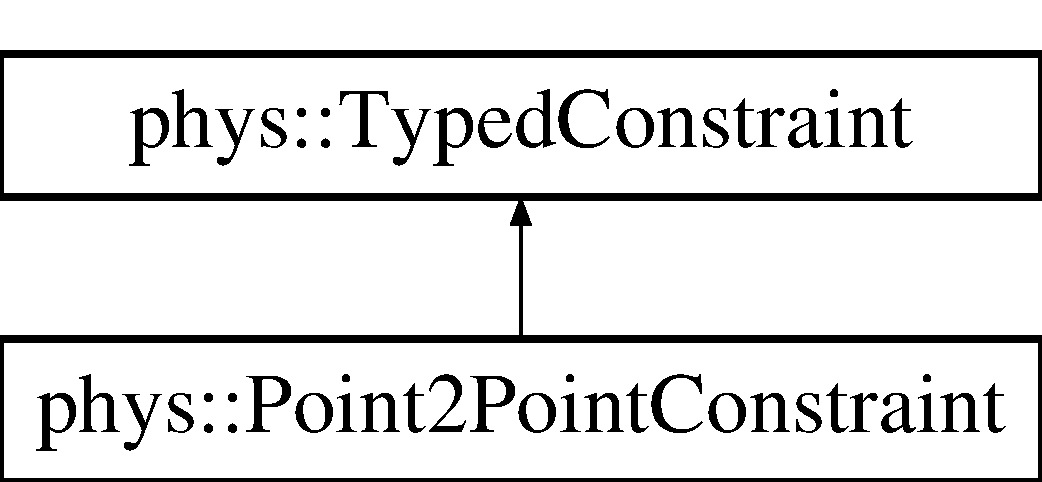
\includegraphics[height=2.000000cm]{classphys_1_1Point2PointConstraint}
\end{center}
\end{figure}
\subsubsection*{Public Member Functions}
\begin{DoxyCompactItemize}
\item 
virtual btTypedConstraint $\ast$ \hyperlink{classphys_1_1Point2PointConstraint_afc714f85fa0c26d8520cd72e73a0b199}{GetConstraintBase} () const 
\item 
virtual \hyperlink{namespacephys_af7eb897198d265b8e868f45240230d5f}{Real} \hyperlink{classphys_1_1Point2PointConstraint_a273576b756d2beca5345a2c85d6b0098}{GetDamping} () const 
\begin{DoxyCompactList}\small\item\em Get the current Damping. \item\end{DoxyCompactList}\item 
virtual \hyperlink{namespacephys_af7eb897198d265b8e868f45240230d5f}{Real} \hyperlink{classphys_1_1Point2PointConstraint_a2ff8bcbf428b6a3d475dc36f13b28b52}{GetImpulseClamping} () const 
\begin{DoxyCompactList}\small\item\em get the current impulse clamping value \item\end{DoxyCompactList}\item 
virtual \hyperlink{classphys_1_1Vector3}{Vector3} \hyperlink{classphys_1_1Point2PointConstraint_a97009ed12b23028241a59e602dc63e38}{GetPivotALocation} () const 
\begin{DoxyCompactList}\small\item\em Get offset of the first actor. \item\end{DoxyCompactList}\item 
virtual \hyperlink{classphys_1_1Vector3}{Vector3} \hyperlink{classphys_1_1Point2PointConstraint_a478b2fc6019b6c0fe57ef41e323b5e63}{GetPivotBLocation} () const 
\begin{DoxyCompactList}\small\item\em Get offset of the second actor. \item\end{DoxyCompactList}\item 
virtual \hyperlink{namespacephys_af7eb897198d265b8e868f45240230d5f}{Real} \hyperlink{classphys_1_1Point2PointConstraint_a9b5ccfef074f8c8df18455f2690c1cd1}{GetTAU} () const 
\begin{DoxyCompactList}\small\item\em Retrieve the Tau Setting. \item\end{DoxyCompactList}\item 
virtual bool \hyperlink{classphys_1_1Point2PointConstraint_a37ba19abafb1fad5a898b22cdd792129}{HasParamBeenSet} (\hyperlink{namespacephys_aa1e7cf2d7efcaeaeac304f711e7564e8}{ConstraintParam} Param, int Axis) const 
\item 
\hyperlink{classphys_1_1Point2PointConstraint_a64806b50332492d3342884f40e7871fb}{Point2PointConstraint} (\hyperlink{classphys_1_1ActorRigid}{ActorRigid} $\ast$ActorA, const \hyperlink{classphys_1_1Vector3}{Vector3} \&PivotA)
\begin{DoxyCompactList}\small\item\em Single body constructor. Binds the body to world space. \item\end{DoxyCompactList}\item 
\hyperlink{classphys_1_1Point2PointConstraint_a890c02b69d2b477e5e7c638c36a8c84d}{Point2PointConstraint} (\hyperlink{classphys_1_1ActorRigid}{ActorRigid} $\ast$ActorA, \hyperlink{classphys_1_1ActorRigid}{ActorRigid} $\ast$ActorB, const \hyperlink{classphys_1_1Vector3}{Vector3} \&PivotA, const \hyperlink{classphys_1_1Vector3}{Vector3} \&PivotB)
\begin{DoxyCompactList}\small\item\em Double body constructor. Binds the two bodies. \item\end{DoxyCompactList}\item 
virtual void \hyperlink{classphys_1_1Point2PointConstraint_a1ba1bd6cc8d16c69579633f0a5b28b6d}{ProtoDeSerialize} (const \hyperlink{classphys_1_1xml_1_1Node}{xml::Node} \&OneNode)
\begin{DoxyCompactList}\small\item\em Take the data stored in an XML and overwrite this instance of this object with it. \item\end{DoxyCompactList}\item 
virtual void \hyperlink{classphys_1_1Point2PointConstraint_ace2e182da3c1495084eea1a5fcc97cfd}{ProtoSerialize} (\hyperlink{classphys_1_1xml_1_1Node}{xml::Node} \&CurrentRoot) const 
\begin{DoxyCompactList}\small\item\em Convert this class to an \hyperlink{classphys_1_1xml_1_1Node}{xml::Node} ready for serialization. \item\end{DoxyCompactList}\item 
\hyperlink{namespacephys_aa03900411993de7fbfec4789bc1d392e}{String} \hyperlink{classphys_1_1Point2PointConstraint_ae658c1f5c370b8a4cf94fcf276696dbf}{SerializableName} () const 
\begin{DoxyCompactList}\small\item\em Get the name of the the XML tag this class will leave behind as its instances are serialized. \item\end{DoxyCompactList}\item 
virtual void \hyperlink{classphys_1_1Point2PointConstraint_a4699d58e8ec97e5eafa12508e89fa878}{SetDamping} (\hyperlink{namespacephys_af7eb897198d265b8e868f45240230d5f}{Real} Damping)
\begin{DoxyCompactList}\small\item\em Set a resistive force against the constraint, not too dissimilar to from hinge friction or Air resistance. \item\end{DoxyCompactList}\item 
virtual void \hyperlink{classphys_1_1Point2PointConstraint_afd2be426f4a13b9512d964903a035551}{SetImpulseClamping} (\hyperlink{namespacephys_af7eb897198d265b8e868f45240230d5f}{Real} Clamping)
\begin{DoxyCompactList}\small\item\em Set the current impulse clamping on the constraint. \item\end{DoxyCompactList}\item 
virtual void \hyperlink{classphys_1_1Point2PointConstraint_ad1ffe9d877dd0601f76215bec56c1a4a}{SetPivotALocation} (const \hyperlink{classphys_1_1Vector3}{Vector3} \&PivotA)
\begin{DoxyCompactList}\small\item\em Set offset of the first actor. \item\end{DoxyCompactList}\item 
virtual void \hyperlink{classphys_1_1Point2PointConstraint_abb11fffed7284323321be9ff481268a4}{SetPivotBLocation} (const \hyperlink{classphys_1_1Vector3}{Vector3} \&PivotB)
\begin{DoxyCompactList}\small\item\em Set offset of the second actor. \item\end{DoxyCompactList}\item 
virtual void \hyperlink{classphys_1_1Point2PointConstraint_a556c4610b62c075efaa9d246cf3d2dc2}{SetTAU} (\hyperlink{namespacephys_af7eb897198d265b8e868f45240230d5f}{Real} TAU)
\begin{DoxyCompactList}\small\item\em This may be a scalar for how strongly Angular momentum affects linear momemtum. \item\end{DoxyCompactList}\item 
virtual \hyperlink{classphys_1_1TypedConstraint_a26261a4055e84e104c58d84eea5667c2}{TypedConstraint::AxisList} \hyperlink{classphys_1_1Point2PointConstraint_ab33ef9c2b99432247b4582cb829bb9dc}{ValidAngularAxis} () const 
\item 
virtual \hyperlink{classphys_1_1TypedConstraint_a26261a4055e84e104c58d84eea5667c2}{TypedConstraint::AxisList} \hyperlink{classphys_1_1Point2PointConstraint_a7c430ecbfc798d26ddabd66ee66f6a27}{ValidLinearAxis} () const 
\item 
virtual \hyperlink{classphys_1_1TypedConstraint_a4c2dcea3fbb764e454840329126d034e}{TypedConstraint::ParamList} \hyperlink{classphys_1_1Point2PointConstraint_a5ab3a1dac5cabe07f6abfe576090634f}{ValidParamOnAxis} (int Axis) const 
\item 
virtual \hyperlink{classphys_1_1Point2PointConstraint_a6e0bdac8c6ee7612c07b441c7556dc14}{$\sim$Point2PointConstraint} ()
\begin{DoxyCompactList}\small\item\em Class destructor. \item\end{DoxyCompactList}\end{DoxyCompactItemize}
\subsubsection*{Protected Attributes}
\begin{DoxyCompactItemize}
\item 
\hypertarget{classphys_1_1Point2PointConstraint_aa58b7fd9fe368c72d5bc5e1990bdf593}{
btPoint2PointConstraint $\ast$ \hyperlink{classphys_1_1Point2PointConstraint_aa58b7fd9fe368c72d5bc5e1990bdf593}{Point2Point}}
\label{classphys_1_1Point2PointConstraint_aa58b7fd9fe368c72d5bc5e1990bdf593}

\begin{DoxyCompactList}\small\item\em Bullet constraint that this class encapsulates. \item\end{DoxyCompactList}\end{DoxyCompactItemize}


\subsubsection{Detailed Description}
Tries to make a point relative to each of two actors match in 3d space, without regard to rotation. This will translate (push around) the actors to attempt to get the offsets to match up in 3d space. The actors can freely rotate about their relative offsets. 

Definition at line 1194 of file constraint.h.



\subsubsection{Constructor \& Destructor Documentation}
\hypertarget{classphys_1_1Point2PointConstraint_a890c02b69d2b477e5e7c638c36a8c84d}{
\index{phys::Point2PointConstraint@{phys::Point2PointConstraint}!Point2PointConstraint@{Point2PointConstraint}}
\index{Point2PointConstraint@{Point2PointConstraint}!phys::Point2PointConstraint@{phys::Point2PointConstraint}}
\paragraph[{Point2PointConstraint}]{\setlength{\rightskip}{0pt plus 5cm}phys::Point2PointConstraint::Point2PointConstraint (
\begin{DoxyParamCaption}
\item[{{\bf ActorRigid} $\ast$}]{ActorA, }
\item[{{\bf ActorRigid} $\ast$}]{ActorB, }
\item[{const {\bf Vector3} \&}]{PivotA, }
\item[{const {\bf Vector3} \&}]{PivotB}
\end{DoxyParamCaption}
)}\hfill}
\label{classphys_1_1Point2PointConstraint_a890c02b69d2b477e5e7c638c36a8c84d}


Double body constructor. Binds the two bodies. 


\begin{DoxyParams}{Parameters}
{\em ActorA} & The first actor to apply this constraint to. \\
\hline
{\em ActorB} & The second actor to apply this constraint to. \\
\hline
{\em PivotA} & The location in ActorA's local space to apply the constraint to. \\
\hline
{\em PivotB} & The location in ActorB's local space to apply the constraint to. \\
\hline
\end{DoxyParams}
\hypertarget{classphys_1_1Point2PointConstraint_a64806b50332492d3342884f40e7871fb}{
\index{phys::Point2PointConstraint@{phys::Point2PointConstraint}!Point2PointConstraint@{Point2PointConstraint}}
\index{Point2PointConstraint@{Point2PointConstraint}!phys::Point2PointConstraint@{phys::Point2PointConstraint}}
\paragraph[{Point2PointConstraint}]{\setlength{\rightskip}{0pt plus 5cm}phys::Point2PointConstraint::Point2PointConstraint (
\begin{DoxyParamCaption}
\item[{{\bf ActorRigid} $\ast$}]{ActorA, }
\item[{const {\bf Vector3} \&}]{PivotA}
\end{DoxyParamCaption}
)}\hfill}
\label{classphys_1_1Point2PointConstraint_a64806b50332492d3342884f40e7871fb}


Single body constructor. Binds the body to world space. 


\begin{DoxyParams}{Parameters}
{\em ActorA} & The actor to apply this constraint to. \\
\hline
{\em PivotA} & The position relative to ActorA's center of gravity to \char`\"{}Pin\char`\"{} to the world. \\
\hline
\end{DoxyParams}
\hypertarget{classphys_1_1Point2PointConstraint_a6e0bdac8c6ee7612c07b441c7556dc14}{
\index{phys::Point2PointConstraint@{phys::Point2PointConstraint}!$\sim$Point2PointConstraint@{$\sim$Point2PointConstraint}}
\index{$\sim$Point2PointConstraint@{$\sim$Point2PointConstraint}!phys::Point2PointConstraint@{phys::Point2PointConstraint}}
\paragraph[{$\sim$Point2PointConstraint}]{\setlength{\rightskip}{0pt plus 5cm}virtual phys::Point2PointConstraint::$\sim$Point2PointConstraint (
\begin{DoxyParamCaption}
{}
\end{DoxyParamCaption}
)\hspace{0.3cm}{\ttfamily  \mbox{[}virtual\mbox{]}}}\hfill}
\label{classphys_1_1Point2PointConstraint_a6e0bdac8c6ee7612c07b441c7556dc14}


Class destructor. 

The class destructor. 

\subsubsection{Member Function Documentation}
\hypertarget{classphys_1_1Point2PointConstraint_afc714f85fa0c26d8520cd72e73a0b199}{
\index{phys::Point2PointConstraint@{phys::Point2PointConstraint}!GetConstraintBase@{GetConstraintBase}}
\index{GetConstraintBase@{GetConstraintBase}!phys::Point2PointConstraint@{phys::Point2PointConstraint}}
\paragraph[{GetConstraintBase}]{\setlength{\rightskip}{0pt plus 5cm}virtual btTypedConstraint$\ast$ phys::Point2PointConstraint::GetConstraintBase (
\begin{DoxyParamCaption}
{}
\end{DoxyParamCaption}
) const\hspace{0.3cm}{\ttfamily  \mbox{[}virtual\mbox{]}}}\hfill}
\label{classphys_1_1Point2PointConstraint_afc714f85fa0c26d8520cd72e73a0b199}
Get the Bullet constraint that this class encapsulates. 

\begin{DoxyReturn}{Returns}
A pointer to the btTypedConstraint that stores the underlying constraint. 
\end{DoxyReturn}
 

Implements \hyperlink{classphys_1_1TypedConstraint_ab3bd2baa58d3f0d812401cbf59159a8b}{phys::TypedConstraint}.

\hypertarget{classphys_1_1Point2PointConstraint_a273576b756d2beca5345a2c85d6b0098}{
\index{phys::Point2PointConstraint@{phys::Point2PointConstraint}!GetDamping@{GetDamping}}
\index{GetDamping@{GetDamping}!phys::Point2PointConstraint@{phys::Point2PointConstraint}}
\paragraph[{GetDamping}]{\setlength{\rightskip}{0pt plus 5cm}virtual {\bf Real} phys::Point2PointConstraint::GetDamping (
\begin{DoxyParamCaption}
{}
\end{DoxyParamCaption}
) const\hspace{0.3cm}{\ttfamily  \mbox{[}virtual\mbox{]}}}\hfill}
\label{classphys_1_1Point2PointConstraint_a273576b756d2beca5345a2c85d6b0098}


Get the current Damping. 

\begin{DoxyReturn}{Returns}
A Real with the Damping value. 
\end{DoxyReturn}
\hypertarget{classphys_1_1Point2PointConstraint_a2ff8bcbf428b6a3d475dc36f13b28b52}{
\index{phys::Point2PointConstraint@{phys::Point2PointConstraint}!GetImpulseClamping@{GetImpulseClamping}}
\index{GetImpulseClamping@{GetImpulseClamping}!phys::Point2PointConstraint@{phys::Point2PointConstraint}}
\paragraph[{GetImpulseClamping}]{\setlength{\rightskip}{0pt plus 5cm}virtual {\bf Real} phys::Point2PointConstraint::GetImpulseClamping (
\begin{DoxyParamCaption}
{}
\end{DoxyParamCaption}
) const\hspace{0.3cm}{\ttfamily  \mbox{[}virtual\mbox{]}}}\hfill}
\label{classphys_1_1Point2PointConstraint_a2ff8bcbf428b6a3d475dc36f13b28b52}


get the current impulse clamping value 

\begin{DoxyReturn}{Returns}
A real with the Clamping 
\end{DoxyReturn}
\hypertarget{classphys_1_1Point2PointConstraint_a97009ed12b23028241a59e602dc63e38}{
\index{phys::Point2PointConstraint@{phys::Point2PointConstraint}!GetPivotALocation@{GetPivotALocation}}
\index{GetPivotALocation@{GetPivotALocation}!phys::Point2PointConstraint@{phys::Point2PointConstraint}}
\paragraph[{GetPivotALocation}]{\setlength{\rightskip}{0pt plus 5cm}virtual {\bf Vector3} phys::Point2PointConstraint::GetPivotALocation (
\begin{DoxyParamCaption}
{}
\end{DoxyParamCaption}
) const\hspace{0.3cm}{\ttfamily  \mbox{[}virtual\mbox{]}}}\hfill}
\label{classphys_1_1Point2PointConstraint_a97009ed12b23028241a59e602dc63e38}


Get offset of the first actor. 

\begin{DoxyReturn}{Returns}
The offset as a \hyperlink{classphys_1_1Vector3}{Vector3} relative to the center of mass of ActorA. 
\end{DoxyReturn}


Implements \hyperlink{classphys_1_1TypedConstraint_af9827f1d4c7bcfb201d43d3dcf03cdfd}{phys::TypedConstraint}.

\hypertarget{classphys_1_1Point2PointConstraint_a478b2fc6019b6c0fe57ef41e323b5e63}{
\index{phys::Point2PointConstraint@{phys::Point2PointConstraint}!GetPivotBLocation@{GetPivotBLocation}}
\index{GetPivotBLocation@{GetPivotBLocation}!phys::Point2PointConstraint@{phys::Point2PointConstraint}}
\paragraph[{GetPivotBLocation}]{\setlength{\rightskip}{0pt plus 5cm}virtual {\bf Vector3} phys::Point2PointConstraint::GetPivotBLocation (
\begin{DoxyParamCaption}
{}
\end{DoxyParamCaption}
) const\hspace{0.3cm}{\ttfamily  \mbox{[}virtual\mbox{]}}}\hfill}
\label{classphys_1_1Point2PointConstraint_a478b2fc6019b6c0fe57ef41e323b5e63}


Get offset of the second actor. 

\begin{DoxyReturn}{Returns}
The offset as a \hyperlink{classphys_1_1Vector3}{Vector3} relative to the center of mass of ActorB. 
\end{DoxyReturn}


Implements \hyperlink{classphys_1_1TypedConstraint_ad1d8e9e2ab17579bd6c13ee8c4acf20b}{phys::TypedConstraint}.

\hypertarget{classphys_1_1Point2PointConstraint_a9b5ccfef074f8c8df18455f2690c1cd1}{
\index{phys::Point2PointConstraint@{phys::Point2PointConstraint}!GetTAU@{GetTAU}}
\index{GetTAU@{GetTAU}!phys::Point2PointConstraint@{phys::Point2PointConstraint}}
\paragraph[{GetTAU}]{\setlength{\rightskip}{0pt plus 5cm}virtual {\bf Real} phys::Point2PointConstraint::GetTAU (
\begin{DoxyParamCaption}
{}
\end{DoxyParamCaption}
) const\hspace{0.3cm}{\ttfamily  \mbox{[}virtual\mbox{]}}}\hfill}
\label{classphys_1_1Point2PointConstraint_a9b5ccfef074f8c8df18455f2690c1cd1}


Retrieve the Tau Setting. 

\begin{DoxyReturn}{Returns}
The Tau value as a Real 
\end{DoxyReturn}
\hypertarget{classphys_1_1Point2PointConstraint_a37ba19abafb1fad5a898b22cdd792129}{
\index{phys::Point2PointConstraint@{phys::Point2PointConstraint}!HasParamBeenSet@{HasParamBeenSet}}
\index{HasParamBeenSet@{HasParamBeenSet}!phys::Point2PointConstraint@{phys::Point2PointConstraint}}
\paragraph[{HasParamBeenSet}]{\setlength{\rightskip}{0pt plus 5cm}virtual bool phys::Point2PointConstraint::HasParamBeenSet (
\begin{DoxyParamCaption}
\item[{{\bf ConstraintParam}}]{Param, }
\item[{int}]{Axis}
\end{DoxyParamCaption}
) const\hspace{0.3cm}{\ttfamily  \mbox{[}virtual\mbox{]}}}\hfill}
\label{classphys_1_1Point2PointConstraint_a37ba19abafb1fad5a898b22cdd792129}
 

Implements \hyperlink{classphys_1_1TypedConstraint_a849e7b91306f444cb8c73d52707a9521}{phys::TypedConstraint}.

\hypertarget{classphys_1_1Point2PointConstraint_a1ba1bd6cc8d16c69579633f0a5b28b6d}{
\index{phys::Point2PointConstraint@{phys::Point2PointConstraint}!ProtoDeSerialize@{ProtoDeSerialize}}
\index{ProtoDeSerialize@{ProtoDeSerialize}!phys::Point2PointConstraint@{phys::Point2PointConstraint}}
\paragraph[{ProtoDeSerialize}]{\setlength{\rightskip}{0pt plus 5cm}virtual void phys::Point2PointConstraint::ProtoDeSerialize (
\begin{DoxyParamCaption}
\item[{const {\bf xml::Node} \&}]{OneNode}
\end{DoxyParamCaption}
)\hspace{0.3cm}{\ttfamily  \mbox{[}virtual\mbox{]}}}\hfill}
\label{classphys_1_1Point2PointConstraint_a1ba1bd6cc8d16c69579633f0a5b28b6d}


Take the data stored in an XML and overwrite this instance of this object with it. 


\begin{DoxyParams}{Parameters}
{\em OneNode} & and \hyperlink{classphys_1_1xml_1_1Node}{xml::Node} containing the data. \\
\hline
\end{DoxyParams}
\begin{DoxyWarning}{Warning}
A precondition of using this is that all of the actors intended for use must already be Deserialized. 
\end{DoxyWarning}


Reimplemented from \hyperlink{classphys_1_1TypedConstraint_aeafb306788de02bfb164806054a1c346}{phys::TypedConstraint}.

\hypertarget{classphys_1_1Point2PointConstraint_ace2e182da3c1495084eea1a5fcc97cfd}{
\index{phys::Point2PointConstraint@{phys::Point2PointConstraint}!ProtoSerialize@{ProtoSerialize}}
\index{ProtoSerialize@{ProtoSerialize}!phys::Point2PointConstraint@{phys::Point2PointConstraint}}
\paragraph[{ProtoSerialize}]{\setlength{\rightskip}{0pt plus 5cm}virtual void phys::Point2PointConstraint::ProtoSerialize (
\begin{DoxyParamCaption}
\item[{{\bf xml::Node} \&}]{CurrentRoot}
\end{DoxyParamCaption}
) const\hspace{0.3cm}{\ttfamily  \mbox{[}virtual\mbox{]}}}\hfill}
\label{classphys_1_1Point2PointConstraint_ace2e182da3c1495084eea1a5fcc97cfd}


Convert this class to an \hyperlink{classphys_1_1xml_1_1Node}{xml::Node} ready for serialization. 


\begin{DoxyParams}{Parameters}
{\em CurrentRoot} & The point in the XML hierarchy that all this vectorw should be appended to. \\
\hline
\end{DoxyParams}


Reimplemented from \hyperlink{classphys_1_1TypedConstraint_a9cf48a2a1afb939cbd03e54ee9be3e0b}{phys::TypedConstraint}.

\hypertarget{classphys_1_1Point2PointConstraint_ae658c1f5c370b8a4cf94fcf276696dbf}{
\index{phys::Point2PointConstraint@{phys::Point2PointConstraint}!SerializableName@{SerializableName}}
\index{SerializableName@{SerializableName}!phys::Point2PointConstraint@{phys::Point2PointConstraint}}
\paragraph[{SerializableName}]{\setlength{\rightskip}{0pt plus 5cm}{\bf String} phys::Point2PointConstraint::SerializableName (
\begin{DoxyParamCaption}
{}
\end{DoxyParamCaption}
) const}\hfill}
\label{classphys_1_1Point2PointConstraint_ae658c1f5c370b8a4cf94fcf276696dbf}


Get the name of the the XML tag this class will leave behind as its instances are serialized. 

\begin{DoxyReturn}{Returns}
A string containing \char`\"{}Point2PointConstraint\char`\"{} 
\end{DoxyReturn}


Reimplemented from \hyperlink{classphys_1_1TypedConstraint_ad604b85a13e3e3b1c01d1c40f678b751}{phys::TypedConstraint}.

\hypertarget{classphys_1_1Point2PointConstraint_a4699d58e8ec97e5eafa12508e89fa878}{
\index{phys::Point2PointConstraint@{phys::Point2PointConstraint}!SetDamping@{SetDamping}}
\index{SetDamping@{SetDamping}!phys::Point2PointConstraint@{phys::Point2PointConstraint}}
\paragraph[{SetDamping}]{\setlength{\rightskip}{0pt plus 5cm}virtual void phys::Point2PointConstraint::SetDamping (
\begin{DoxyParamCaption}
\item[{{\bf Real}}]{Damping}
\end{DoxyParamCaption}
)\hspace{0.3cm}{\ttfamily  \mbox{[}virtual\mbox{]}}}\hfill}
\label{classphys_1_1Point2PointConstraint_a4699d58e8ec97e5eafa12508e89fa878}


Set a resistive force against the constraint, not too dissimilar to from hinge friction or Air resistance. 


\begin{DoxyParams}{Parameters}
{\em Damping} & A real with the desired values \\
\hline
\end{DoxyParams}
\hypertarget{classphys_1_1Point2PointConstraint_afd2be426f4a13b9512d964903a035551}{
\index{phys::Point2PointConstraint@{phys::Point2PointConstraint}!SetImpulseClamping@{SetImpulseClamping}}
\index{SetImpulseClamping@{SetImpulseClamping}!phys::Point2PointConstraint@{phys::Point2PointConstraint}}
\paragraph[{SetImpulseClamping}]{\setlength{\rightskip}{0pt plus 5cm}virtual void phys::Point2PointConstraint::SetImpulseClamping (
\begin{DoxyParamCaption}
\item[{{\bf Real}}]{Clamping}
\end{DoxyParamCaption}
)\hspace{0.3cm}{\ttfamily  \mbox{[}virtual\mbox{]}}}\hfill}
\label{classphys_1_1Point2PointConstraint_afd2be426f4a13b9512d964903a035551}


Set the current impulse clamping on the constraint. 


\begin{DoxyParams}{Parameters}
{\em Clamping} & This is a value that the constraint solver can use to adjust accumlated values when solving the constraint. \\
\hline
\end{DoxyParams}
\hypertarget{classphys_1_1Point2PointConstraint_ad1ffe9d877dd0601f76215bec56c1a4a}{
\index{phys::Point2PointConstraint@{phys::Point2PointConstraint}!SetPivotALocation@{SetPivotALocation}}
\index{SetPivotALocation@{SetPivotALocation}!phys::Point2PointConstraint@{phys::Point2PointConstraint}}
\paragraph[{SetPivotALocation}]{\setlength{\rightskip}{0pt plus 5cm}virtual void phys::Point2PointConstraint::SetPivotALocation (
\begin{DoxyParamCaption}
\item[{const {\bf Vector3} \&}]{PivotA}
\end{DoxyParamCaption}
)\hspace{0.3cm}{\ttfamily  \mbox{[}virtual\mbox{]}}}\hfill}
\label{classphys_1_1Point2PointConstraint_ad1ffe9d877dd0601f76215bec56c1a4a}


Set offset of the first actor. 


\begin{DoxyParams}{Parameters}
{\em PivotA} & The offset as a \hyperlink{classphys_1_1Vector3}{Vector3} relative to the center of mass of ActorA. \\
\hline
\end{DoxyParams}


Implements \hyperlink{classphys_1_1TypedConstraint_aaa301fee77aa6e20ab202f604f0e9518}{phys::TypedConstraint}.

\hypertarget{classphys_1_1Point2PointConstraint_abb11fffed7284323321be9ff481268a4}{
\index{phys::Point2PointConstraint@{phys::Point2PointConstraint}!SetPivotBLocation@{SetPivotBLocation}}
\index{SetPivotBLocation@{SetPivotBLocation}!phys::Point2PointConstraint@{phys::Point2PointConstraint}}
\paragraph[{SetPivotBLocation}]{\setlength{\rightskip}{0pt plus 5cm}virtual void phys::Point2PointConstraint::SetPivotBLocation (
\begin{DoxyParamCaption}
\item[{const {\bf Vector3} \&}]{PivotB}
\end{DoxyParamCaption}
)\hspace{0.3cm}{\ttfamily  \mbox{[}virtual\mbox{]}}}\hfill}
\label{classphys_1_1Point2PointConstraint_abb11fffed7284323321be9ff481268a4}


Set offset of the second actor. 


\begin{DoxyParams}{Parameters}
{\em PivotB} & The offset as a \hyperlink{classphys_1_1Vector3}{Vector3} relative to the center of mass of ActorB. \\
\hline
\end{DoxyParams}


Implements \hyperlink{classphys_1_1TypedConstraint_a518b3a40e517e21da8049e645a69fc96}{phys::TypedConstraint}.

\hypertarget{classphys_1_1Point2PointConstraint_a556c4610b62c075efaa9d246cf3d2dc2}{
\index{phys::Point2PointConstraint@{phys::Point2PointConstraint}!SetTAU@{SetTAU}}
\index{SetTAU@{SetTAU}!phys::Point2PointConstraint@{phys::Point2PointConstraint}}
\paragraph[{SetTAU}]{\setlength{\rightskip}{0pt plus 5cm}virtual void phys::Point2PointConstraint::SetTAU (
\begin{DoxyParamCaption}
\item[{{\bf Real}}]{TAU}
\end{DoxyParamCaption}
)\hspace{0.3cm}{\ttfamily  \mbox{[}virtual\mbox{]}}}\hfill}
\label{classphys_1_1Point2PointConstraint_a556c4610b62c075efaa9d246cf3d2dc2}


This may be a scalar for how strongly Angular momentum affects linear momemtum. 

\begin{Desc}
\item[\hyperlink{todo__todo000004}{Todo}]Research this more carefully \end{Desc}


This function is a tightly wrapped bullet 3d function. No real documentation for it exists, from its responsibility/location in Bullet3d and a basic understanding of torque ( see \href{http://en.wikipedia.org/wiki/Torque}{\tt http://en.wikipedia.org/wiki/Torque} ) It is highly likely that it is a value to adjust how torque affects momentum. \hypertarget{classphys_1_1Point2PointConstraint_ab33ef9c2b99432247b4582cb829bb9dc}{
\index{phys::Point2PointConstraint@{phys::Point2PointConstraint}!ValidAngularAxis@{ValidAngularAxis}}
\index{ValidAngularAxis@{ValidAngularAxis}!phys::Point2PointConstraint@{phys::Point2PointConstraint}}
\paragraph[{ValidAngularAxis}]{\setlength{\rightskip}{0pt plus 5cm}virtual {\bf TypedConstraint::AxisList} phys::Point2PointConstraint::ValidAngularAxis (
\begin{DoxyParamCaption}
{}
\end{DoxyParamCaption}
) const\hspace{0.3cm}{\ttfamily  \mbox{[}virtual\mbox{]}}}\hfill}
\label{classphys_1_1Point2PointConstraint_ab33ef9c2b99432247b4582cb829bb9dc}
Get A list sorted (low to high) of all axis that operate Angularly (that lock sliding/translation) 

\begin{DoxyWarning}{Warning}
Odd behaviors, maybe even undefined behavior can happen if This returns a matching Axis to a Linear Axis. Any given axis should only be one or the other 
\end{DoxyWarning}
\begin{DoxyReturn}{Returns}
An Axislist with the Axis this constraint Angularly supports. 
\end{DoxyReturn}
 

Implements \hyperlink{classphys_1_1TypedConstraint_afd67483ff73a4b8ffef17c149b8a6cfa}{phys::TypedConstraint}.

\hypertarget{classphys_1_1Point2PointConstraint_a7c430ecbfc798d26ddabd66ee66f6a27}{
\index{phys::Point2PointConstraint@{phys::Point2PointConstraint}!ValidLinearAxis@{ValidLinearAxis}}
\index{ValidLinearAxis@{ValidLinearAxis}!phys::Point2PointConstraint@{phys::Point2PointConstraint}}
\paragraph[{ValidLinearAxis}]{\setlength{\rightskip}{0pt plus 5cm}virtual {\bf TypedConstraint::AxisList} phys::Point2PointConstraint::ValidLinearAxis (
\begin{DoxyParamCaption}
{}
\end{DoxyParamCaption}
) const\hspace{0.3cm}{\ttfamily  \mbox{[}virtual\mbox{]}}}\hfill}
\label{classphys_1_1Point2PointConstraint_a7c430ecbfc798d26ddabd66ee66f6a27}
Get a sorted (low to high) list of all axis that operate linearly (that lock sliding/translation) 

\begin{DoxyWarning}{Warning}
Odd behaviors, maybe even undefined behavior can happen if This returns a matching Axis to a Linear Axis. Any given axis should only be one or the other 
\end{DoxyWarning}
\begin{DoxyReturn}{Returns}
An Axislist with the Axis this constraint linearly supports. 
\end{DoxyReturn}
 

Implements \hyperlink{classphys_1_1TypedConstraint_af9d5a6630d5f384825388a1e73c88b3a}{phys::TypedConstraint}.

\hypertarget{classphys_1_1Point2PointConstraint_a5ab3a1dac5cabe07f6abfe576090634f}{
\index{phys::Point2PointConstraint@{phys::Point2PointConstraint}!ValidParamOnAxis@{ValidParamOnAxis}}
\index{ValidParamOnAxis@{ValidParamOnAxis}!phys::Point2PointConstraint@{phys::Point2PointConstraint}}
\paragraph[{ValidParamOnAxis}]{\setlength{\rightskip}{0pt plus 5cm}virtual {\bf TypedConstraint::ParamList} phys::Point2PointConstraint::ValidParamOnAxis (
\begin{DoxyParamCaption}
\item[{int}]{Axis}
\end{DoxyParamCaption}
) const\hspace{0.3cm}{\ttfamily  \mbox{[}virtual\mbox{]}}}\hfill}
\label{classphys_1_1Point2PointConstraint_a5ab3a1dac5cabe07f6abfe576090634f}
Get a sorted (low to high) list of Parameters that are valid on this Axis. 

Parameters returned from this will work on the given axis even if they are not valid on any other axis. There is no guarantee that the Parameters will be uniquely stored per an axis. There is no guarantee that changing one parameter will not change another. 
\begin{DoxyParams}{Parameters}
{\em Axis} & the Axis to check. \\
\hline
\end{DoxyParams}
\begin{DoxyReturn}{Returns}
A Paramlist with all the valid parameters for this axis. 
\end{DoxyReturn}
 

Implements \hyperlink{classphys_1_1TypedConstraint_af9f4c03dbba0d55e60dce341dbdc1105}{phys::TypedConstraint}.



The documentation for this class was generated from the following file:\begin{DoxyCompactItemize}
\item 
constraint.h\end{DoxyCompactItemize}

\hypertarget{classphys_1_1Quaternion}{
\subsection{phys::Quaternion Class Reference}
\label{classphys_1_1Quaternion}\index{phys::Quaternion@{phys::Quaternion}}
}


This is used to store information about rotation in 3d space.  




{\ttfamily \#include $<$quaternion.h$>$}

\subsubsection*{Public Member Functions}
\begin{DoxyCompactItemize}
\item 
\hyperlink{namespacephys_af7eb897198d265b8e868f45240230d5f}{Real} \hyperlink{classphys_1_1Quaternion_a249938e4221bf91c0853d7ff28b42392}{DotProduct} (const \hyperlink{classphys_1_1Quaternion}{Quaternion} \&Other) const 
\begin{DoxyCompactList}\small\item\em Gets the Dot Product of this quaternion and another quaternion. \item\end{DoxyCompactList}\item 
void \hyperlink{classphys_1_1Quaternion_a10d3582b2731e70279d7bab43173f317}{ExtractBulletQuaternion} (const btQuaternion \&Ours)
\begin{DoxyCompactList}\small\item\em Copies an existing Bullet quaternion. \item\end{DoxyCompactList}\item 
void \hyperlink{classphys_1_1Quaternion_a942fab675a0b124e1dc5e2febab113e6}{ExtractOgreQuaternion} (const Ogre::Quaternion \&Ours)
\begin{DoxyCompactList}\small\item\em Copies an existing Ogre quaternion. \item\end{DoxyCompactList}\item 
btQuaternion \hyperlink{classphys_1_1Quaternion_a053f994770b600ae153a142bb4ba7d33}{GetBulletQuaternion} (bool normalize=false) const 
\begin{DoxyCompactList}\small\item\em Gets a Bullet quaternion. \item\end{DoxyCompactList}\item 
\hyperlink{classphys_1_1Quaternion}{Quaternion} \hyperlink{classphys_1_1Quaternion_a384833001b14c132553af190e6ebc41e}{GetInverse} () const 
\begin{DoxyCompactList}\small\item\em Inverses this \hyperlink{classphys_1_1Quaternion}{Quaternion}. \item\end{DoxyCompactList}\item 
\hyperlink{classphys_1_1Quaternion}{Quaternion} \hyperlink{classphys_1_1Quaternion_a70d6cf4b57f3e74469089747ef755583}{GetNormalizedCopy} ()
\begin{DoxyCompactList}\small\item\em Get a normalized copy of this \hyperlink{classphys_1_1Quaternion}{Quaternion} without changing this one. \item\end{DoxyCompactList}\item 
Ogre::Quaternion \hyperlink{classphys_1_1Quaternion_aa22645e2e2972007bcf61cd2f8e506d0}{GetOgreQuaternion} (bool normalize=false) const 
\begin{DoxyCompactList}\small\item\em Gets a Ogre quaternion. \item\end{DoxyCompactList}\item 
\hyperlink{namespacephys_af7eb897198d265b8e868f45240230d5f}{Real} \hyperlink{classphys_1_1Quaternion_aaa860619e9370244d1b538dd9aaf0efc}{Length} () const 
\begin{DoxyCompactList}\small\item\em Gets the length of the quaternion. \item\end{DoxyCompactList}\item 
\hyperlink{namespacephys_af7eb897198d265b8e868f45240230d5f}{Real} \hyperlink{classphys_1_1Quaternion_ac81b52051cc7dcb73fa01fb963d068a6}{LengthSqrd} () const 
\begin{DoxyCompactList}\small\item\em Gets the squared length(len$^\wedge$2) of the quaternion. \item\end{DoxyCompactList}\item 
\hyperlink{classphys_1_1Quaternion}{Quaternion} \& \hyperlink{classphys_1_1Quaternion_afafa852e782d0fe20d41bc745c8a4734}{Normalize} ()
\begin{DoxyCompactList}\small\item\em Normalizes this \hyperlink{classphys_1_1Quaternion}{Quaternion}. \item\end{DoxyCompactList}\item 
\hyperlink{classphys_1_1Quaternion}{Quaternion} \hyperlink{classphys_1_1Quaternion_a8a67c3e05a56a38407f899020c61631d}{operator$\ast$} (const \hyperlink{namespacephys_af7eb897198d265b8e868f45240230d5f}{Real} \&Scalar) const 
\begin{DoxyCompactList}\small\item\em Scaling by multiplication. \item\end{DoxyCompactList}\item 
\hyperlink{classphys_1_1Quaternion}{Quaternion} \hyperlink{classphys_1_1Quaternion_a2b1017fc916a896440a00bee3fd3ca9b}{operator$\ast$} (const \hyperlink{classphys_1_1Quaternion}{phys::Quaternion} \&Other) const 
\begin{DoxyCompactList}\small\item\em Multiplication operator with \hyperlink{classphys_1_1Quaternion}{phys::Quaternion} and \hyperlink{classphys_1_1Quaternion}{phys::Quaternion}. \item\end{DoxyCompactList}\item 
\hyperlink{classphys_1_1Quaternion}{Quaternion} \hyperlink{classphys_1_1Quaternion_ae37df9d07e51739908e05a4bd518c1e1}{operator$\ast$} (const Ogre::Quaternion \&Other) const 
\begin{DoxyCompactList}\small\item\em Multiplication operator with \hyperlink{classphys_1_1Quaternion}{phys::Quaternion} and Ogre::Quaternion. \item\end{DoxyCompactList}\item 
\hyperlink{classphys_1_1Quaternion}{Quaternion} \hyperlink{classphys_1_1Quaternion_abafe5f21ebfac271310905b29da13373}{operator$\ast$} (const btQuaternion \&Other) const 
\begin{DoxyCompactList}\small\item\em Multiplication operator with \hyperlink{classphys_1_1Quaternion}{phys::Quaternion} and btQuaternion. \item\end{DoxyCompactList}\item 
\hyperlink{classphys_1_1Vector3}{Vector3} \hyperlink{classphys_1_1Quaternion_a4e3107c95f94d2b4ddae8c86be9fe28e}{operator$\ast$} (const \hyperlink{classphys_1_1Vector3}{Vector3} \&Other) const 
\begin{DoxyCompactList}\small\item\em Rotates a vector by the provided vector. \item\end{DoxyCompactList}\item 
\hyperlink{classphys_1_1Quaternion}{Quaternion} \hyperlink{classphys_1_1Quaternion_af3f9a9b5835400dc5b83ba06bf9845b0}{operator+} (const \hyperlink{classphys_1_1Quaternion}{phys::Quaternion} \&Other) const 
\begin{DoxyCompactList}\small\item\em Addition operator with \hyperlink{classphys_1_1Quaternion}{phys::Quaternion} and \hyperlink{classphys_1_1Quaternion}{phys::Quaternion}. \item\end{DoxyCompactList}\item 
\hyperlink{classphys_1_1Quaternion}{Quaternion} \hyperlink{classphys_1_1Quaternion_a71fcb37dae7602349e856b202ca00e89}{operator+} (const Ogre::Quaternion \&Other) const 
\begin{DoxyCompactList}\small\item\em Addition operator with \hyperlink{classphys_1_1Quaternion}{phys::Quaternion} and Ogre::Quaternion. \item\end{DoxyCompactList}\item 
\hyperlink{classphys_1_1Quaternion}{Quaternion} \hyperlink{classphys_1_1Quaternion_a3dc35eeb41c43ce79fdf2fc64fc15532}{operator+} (const btQuaternion \&Other) const 
\begin{DoxyCompactList}\small\item\em Addition operator with \hyperlink{classphys_1_1Quaternion}{phys::Quaternion} and btQuaternion. \item\end{DoxyCompactList}\item 
\hyperlink{classphys_1_1Quaternion}{Quaternion} \& \hyperlink{classphys_1_1Quaternion_ab167530770fb0463c5473b5f533db9a8}{operator+=} (const btQuaternion \&Other)
\begin{DoxyCompactList}\small\item\em Incrementing operator with \hyperlink{classphys_1_1Quaternion}{phys::Quaternion} and btQuaternion. \item\end{DoxyCompactList}\item 
\hyperlink{classphys_1_1Quaternion}{Quaternion} \& \hyperlink{classphys_1_1Quaternion_a5d9d2ee516e4e142417b21eecf2e94ce}{operator+=} (const \hyperlink{classphys_1_1Quaternion}{phys::Quaternion} \&Other)
\begin{DoxyCompactList}\small\item\em Incrementing operator with \hyperlink{classphys_1_1Quaternion}{phys::Quaternion} and \hyperlink{classphys_1_1Quaternion}{phys::Quaternion}. \item\end{DoxyCompactList}\item 
\hyperlink{classphys_1_1Quaternion}{Quaternion} \& \hyperlink{classphys_1_1Quaternion_ada6772fd05ec9c8d50b8a25ece3d1c5b}{operator+=} (const Ogre::Quaternion \&Other)
\begin{DoxyCompactList}\small\item\em Incrementing operator with \hyperlink{classphys_1_1Quaternion}{phys::Quaternion} and Ogre::Quaternion. \item\end{DoxyCompactList}\item 
\hyperlink{classphys_1_1Quaternion}{Quaternion} \hyperlink{classphys_1_1Quaternion_abab2d787eefc90bbc6710091a5a79234}{operator-\/} (const \hyperlink{classphys_1_1Quaternion}{phys::Quaternion} \&Other) const 
\begin{DoxyCompactList}\small\item\em Subtraction operator with \hyperlink{classphys_1_1Quaternion}{phys::Quaternion} and \hyperlink{classphys_1_1Quaternion}{phys::Quaternion}. \item\end{DoxyCompactList}\item 
\hyperlink{classphys_1_1Quaternion}{Quaternion} \hyperlink{classphys_1_1Quaternion_a01c5412ce8f1ebb212c9afd7e19feb1e}{operator-\/} (const Ogre::Quaternion \&Other) const 
\begin{DoxyCompactList}\small\item\em Subtraction operator with \hyperlink{classphys_1_1Quaternion}{phys::Quaternion} and Ogre::Quaternion. \item\end{DoxyCompactList}\item 
\hyperlink{classphys_1_1Quaternion}{Quaternion} \hyperlink{classphys_1_1Quaternion_aca49f84681f836545c30c0b42480dccc}{operator-\/} (const btQuaternion \&Other) const 
\begin{DoxyCompactList}\small\item\em Subtraction operator with \hyperlink{classphys_1_1Quaternion}{phys::Quaternion} and btQuaternion. \item\end{DoxyCompactList}\item 
\hyperlink{classphys_1_1Quaternion}{Quaternion} \& \hyperlink{classphys_1_1Quaternion_a66086148dd9154e3e3e0b46bacafe0f7}{operator-\/=} (const \hyperlink{classphys_1_1Quaternion}{phys::Quaternion} \&Other)
\begin{DoxyCompactList}\small\item\em Decrementing operator with \hyperlink{classphys_1_1Quaternion}{phys::Quaternion} and \hyperlink{classphys_1_1Quaternion}{phys::Quaternion}. \item\end{DoxyCompactList}\item 
\hyperlink{classphys_1_1Quaternion}{Quaternion} \& \hyperlink{classphys_1_1Quaternion_af62037687eea0005c9fc4a09355656ed}{operator-\/=} (const Ogre::Quaternion \&Other)
\begin{DoxyCompactList}\small\item\em Decrementing operator with \hyperlink{classphys_1_1Quaternion}{phys::Quaternion} and Ogre::Quaternion. \item\end{DoxyCompactList}\item 
\hyperlink{classphys_1_1Quaternion}{Quaternion} \& \hyperlink{classphys_1_1Quaternion_abd1e9d740b3af194c60466105d07f6ff}{operator-\/=} (const btQuaternion \&Other)
\begin{DoxyCompactList}\small\item\em Decrementing operator with \hyperlink{classphys_1_1Quaternion}{phys::Quaternion} and btQuaternion. \item\end{DoxyCompactList}\item 
\hyperlink{classphys_1_1Quaternion}{Quaternion} \hyperlink{classphys_1_1Quaternion_a9b9492e5a14178aedc784e93b0153364}{operator/} (const \hyperlink{namespacephys_af7eb897198d265b8e868f45240230d5f}{Real} \&Scalar) const 
\begin{DoxyCompactList}\small\item\em Scaling by division. \item\end{DoxyCompactList}\item 
\hyperlink{classphys_1_1Quaternion}{Quaternion} \& \hyperlink{classphys_1_1Quaternion_a6b9fe92548e3fd114d7419ddd5d5a660}{operator=} (const Ogre::Quaternion \&Other)
\begin{DoxyCompactList}\small\item\em Assignment Operator from Ogre::Quaternion. \item\end{DoxyCompactList}\item 
\hyperlink{classphys_1_1Quaternion}{Quaternion} \& \hyperlink{classphys_1_1Quaternion_a05e7364791bf7f38ad63dc59184cd5ca}{operator=} (const btQuaternion \&Other)
\begin{DoxyCompactList}\small\item\em Assignment Operator from btQuaternion. \item\end{DoxyCompactList}\item 
\hyperlink{classphys_1_1Quaternion}{Quaternion} \& \hyperlink{classphys_1_1Quaternion_a6213bddf8f928a8510260b9deb712fd7}{operator=} (const \hyperlink{classphys_1_1Quaternion}{phys::Quaternion} \&Other)
\begin{DoxyCompactList}\small\item\em Assignment Operator from \hyperlink{classphys_1_1Quaternion}{phys::Quaternion}. \item\end{DoxyCompactList}\item 
bool \hyperlink{classphys_1_1Quaternion_a652ec257cb1ab788db646b85f3f89af3}{operator==} (const btQuaternion \&Other) const 
\begin{DoxyCompactList}\small\item\em Equality Comparison Operator from btQuaternion. \item\end{DoxyCompactList}\item 
bool \hyperlink{classphys_1_1Quaternion_a75ab11099a0479885ae5f42945621ef9}{operator==} (const Ogre::Quaternion \&Other) const 
\begin{DoxyCompactList}\small\item\em Equality Comparison Operator from Ogre::Quaternion. \item\end{DoxyCompactList}\item 
bool \hyperlink{classphys_1_1Quaternion_aa02dc20b4246e16017b70788449d7012}{operator==} (const \hyperlink{classphys_1_1Quaternion}{phys::Quaternion} \&Other) const 
\begin{DoxyCompactList}\small\item\em Equality Comparison Operator from \hyperlink{classphys_1_1Quaternion}{phys::Quaternion}. \item\end{DoxyCompactList}\item 
virtual void \hyperlink{classphys_1_1Quaternion_a71e3d4afb129ff822edbc700bae16b4b}{ProtoDeSerialize} (const \hyperlink{classphys_1_1xml_1_1Node}{xml::Node} \&OneNode)
\begin{DoxyCompactList}\small\item\em Take the data stored in an XML and overwrite this instance of this object with it. \item\end{DoxyCompactList}\item 
virtual void \hyperlink{classphys_1_1Quaternion_ab71a780a5103681126d04fec42cdcb2e}{ProtoSerialize} (\hyperlink{classphys_1_1xml_1_1Node}{xml::Node} \&CurrentRoot) const 
\begin{DoxyCompactList}\small\item\em Convert this class to an \hyperlink{classphys_1_1xml_1_1Node}{xml::Node} ready for serialization. \item\end{DoxyCompactList}\item 
\hyperlink{classphys_1_1Quaternion_aca4ee6fd6d3967f06cc4a32361fa5a62}{Quaternion} ()
\begin{DoxyCompactList}\small\item\em Blank Constructor. \item\end{DoxyCompactList}\item 
\hyperlink{classphys_1_1Quaternion_ab9f13d19fe7d602d7c5feaed0aaf4620}{Quaternion} (const btQuaternion \&Theirs)
\begin{DoxyCompactList}\small\item\em Bullet \hyperlink{classphys_1_1Quaternion}{Quaternion} constructor. \item\end{DoxyCompactList}\item 
\hyperlink{classphys_1_1Quaternion_a4902c05489ebae03a55433d947c53d03}{Quaternion} (const Ogre::Quaternion \&Theirs)
\begin{DoxyCompactList}\small\item\em Ogre \hyperlink{classphys_1_1Quaternion}{Quaternion} constructor. \item\end{DoxyCompactList}\item 
\hyperlink{classphys_1_1Quaternion_a46d08f43b0b638a256344b3919ba9e0d}{Quaternion} (const \hyperlink{classphys_1_1Quaternion}{phys::Quaternion} \&Other)
\begin{DoxyCompactList}\small\item\em Copy Constructor. \item\end{DoxyCompactList}\item 
\hyperlink{classphys_1_1Quaternion_ac8037875c08ce10c0195f3e6fd08b172}{Quaternion} (const \hyperlink{namespacephys_af7eb897198d265b8e868f45240230d5f}{Real} \&x, const \hyperlink{namespacephys_af7eb897198d265b8e868f45240230d5f}{Real} \&y, const \hyperlink{namespacephys_af7eb897198d265b8e868f45240230d5f}{Real} \&z, const \hyperlink{namespacephys_af7eb897198d265b8e868f45240230d5f}{Real} \&w)
\begin{DoxyCompactList}\small\item\em Constructor. \item\end{DoxyCompactList}\item 
\hyperlink{classphys_1_1Quaternion_a9246247b7b28f19839148415a7ddeb96}{Quaternion} (const \hyperlink{namespacephys_af7eb897198d265b8e868f45240230d5f}{Real} \&Angle, const \hyperlink{classphys_1_1Vector3}{Vector3} \&Axis)
\begin{DoxyCompactList}\small\item\em Axis and Rotation Constructor. \item\end{DoxyCompactList}\item 
\hyperlink{namespacephys_aa03900411993de7fbfec4789bc1d392e}{String} \hyperlink{classphys_1_1Quaternion_abdfe885d36a7f3c2849a846214fb2872}{SerializableName} () const 
\begin{DoxyCompactList}\small\item\em Get the name of the the XML tag this class will leave behind as its instances are serialized. \item\end{DoxyCompactList}\end{DoxyCompactItemize}
\subsubsection*{Public Attributes}
\begin{DoxyCompactItemize}
\item 
\hypertarget{classphys_1_1Quaternion_af509194048d0cd8fb03d45f150afaa0c}{
\hyperlink{namespacephys_af7eb897198d265b8e868f45240230d5f}{Real} \hyperlink{classphys_1_1Quaternion_af509194048d0cd8fb03d45f150afaa0c}{W}}
\label{classphys_1_1Quaternion_af509194048d0cd8fb03d45f150afaa0c}

\begin{DoxyCompactList}\small\item\em Rotation on the W Axis. \item\end{DoxyCompactList}\item 
\hypertarget{classphys_1_1Quaternion_a29c08e725c7bbb389547cbe03f40f5bd}{
\hyperlink{namespacephys_af7eb897198d265b8e868f45240230d5f}{Real} \hyperlink{classphys_1_1Quaternion_a29c08e725c7bbb389547cbe03f40f5bd}{X}}
\label{classphys_1_1Quaternion_a29c08e725c7bbb389547cbe03f40f5bd}

\begin{DoxyCompactList}\small\item\em Rotation on the X Axis. \item\end{DoxyCompactList}\item 
\hypertarget{classphys_1_1Quaternion_a756165050c3c241fd8b8de6ed21bb268}{
\hyperlink{namespacephys_af7eb897198d265b8e868f45240230d5f}{Real} \hyperlink{classphys_1_1Quaternion_a756165050c3c241fd8b8de6ed21bb268}{Y}}
\label{classphys_1_1Quaternion_a756165050c3c241fd8b8de6ed21bb268}

\begin{DoxyCompactList}\small\item\em Rotation on the Y Axis. \item\end{DoxyCompactList}\item 
\hypertarget{classphys_1_1Quaternion_a708ae111e0cf387b94f33dc7d5b3c59a}{
\hyperlink{namespacephys_af7eb897198d265b8e868f45240230d5f}{Real} \hyperlink{classphys_1_1Quaternion_a708ae111e0cf387b94f33dc7d5b3c59a}{Z}}
\label{classphys_1_1Quaternion_a708ae111e0cf387b94f33dc7d5b3c59a}

\begin{DoxyCompactList}\small\item\em Rotation on the Z Axis. \item\end{DoxyCompactList}\end{DoxyCompactItemize}


\subsubsection{Detailed Description}
This is used to store information about rotation in 3d space. This is used to store information about rotation in 3d space. The X, Y and Z are used to identify a ray from the origin (0,0,0), about which W represents an amount of rotation. \begin{DoxyWarning}{Warning}
The Documentation for this class needs to be revised. It describes 2 mutually exclusive means of storing 
\end{DoxyWarning}


Definition at line 65 of file quaternion.h.



\subsubsection{Constructor \& Destructor Documentation}
\hypertarget{classphys_1_1Quaternion_aca4ee6fd6d3967f06cc4a32361fa5a62}{
\index{phys::Quaternion@{phys::Quaternion}!Quaternion@{Quaternion}}
\index{Quaternion@{Quaternion}!phys::Quaternion@{phys::Quaternion}}
\paragraph[{Quaternion}]{\setlength{\rightskip}{0pt plus 5cm}phys::Quaternion::Quaternion (
\begin{DoxyParamCaption}
{}
\end{DoxyParamCaption}
)}\hfill}
\label{classphys_1_1Quaternion_aca4ee6fd6d3967f06cc4a32361fa5a62}


Blank Constructor. 

Basic no-\/initialization constructor. 

Definition at line 58 of file quaternion.cpp.

\hypertarget{classphys_1_1Quaternion_ac8037875c08ce10c0195f3e6fd08b172}{
\index{phys::Quaternion@{phys::Quaternion}!Quaternion@{Quaternion}}
\index{Quaternion@{Quaternion}!phys::Quaternion@{phys::Quaternion}}
\paragraph[{Quaternion}]{\setlength{\rightskip}{0pt plus 5cm}phys::Quaternion::Quaternion (
\begin{DoxyParamCaption}
\item[{const {\bf Real} \&}]{x, }
\item[{const {\bf Real} \&}]{y, }
\item[{const {\bf Real} \&}]{z, }
\item[{const {\bf Real} \&}]{w}
\end{DoxyParamCaption}
)}\hfill}
\label{classphys_1_1Quaternion_ac8037875c08ce10c0195f3e6fd08b172}


Constructor. 

Constructor that sets all four axis' of rotation. 
\begin{DoxyParams}{Parameters}
{\em x} & Rotation on the X Axis. \\
\hline
{\em y} & Rotation on the Y Axis. \\
\hline
{\em z} & Rotation on the Z Axis. \\
\hline
{\em w} & Rotation on the W Axis. \\
\hline
\end{DoxyParams}


Definition at line 66 of file quaternion.cpp.

\hypertarget{classphys_1_1Quaternion_a9246247b7b28f19839148415a7ddeb96}{
\index{phys::Quaternion@{phys::Quaternion}!Quaternion@{Quaternion}}
\index{Quaternion@{Quaternion}!phys::Quaternion@{phys::Quaternion}}
\paragraph[{Quaternion}]{\setlength{\rightskip}{0pt plus 5cm}phys::Quaternion::Quaternion (
\begin{DoxyParamCaption}
\item[{const {\bf Real} \&}]{Angle, }
\item[{const {\bf Vector3} \&}]{Axis}
\end{DoxyParamCaption}
)}\hfill}
\label{classphys_1_1Quaternion_a9246247b7b28f19839148415a7ddeb96}


Axis and Rotation Constructor. 

This assembles a quaternion based on an axis and a rotation in radians. 
\begin{DoxyParams}{Parameters}
{\em Angle} & Real representing the angle to be applied along the axis in radians. \\
\hline
{\em Axis} & \hyperlink{classphys_1_1Vector3}{Vector3} representing the axis to apply the rotation. \\
\hline
\end{DoxyParams}


\begin{Desc}
\item[\hyperlink{todo__todo000019}{Todo}]Need to find a clean way to wrap sin and cos functions. Also may want to make a radian class/datatype. \end{Desc}




Definition at line 74 of file quaternion.cpp.

\hypertarget{classphys_1_1Quaternion_ab9f13d19fe7d602d7c5feaed0aaf4620}{
\index{phys::Quaternion@{phys::Quaternion}!Quaternion@{Quaternion}}
\index{Quaternion@{Quaternion}!phys::Quaternion@{phys::Quaternion}}
\paragraph[{Quaternion}]{\setlength{\rightskip}{0pt plus 5cm}phys::Quaternion::Quaternion (
\begin{DoxyParamCaption}
\item[{const btQuaternion \&}]{Theirs}
\end{DoxyParamCaption}
)\hspace{0.3cm}{\ttfamily  \mbox{[}explicit\mbox{]}}}\hfill}
\label{classphys_1_1Quaternion_ab9f13d19fe7d602d7c5feaed0aaf4620}


Bullet \hyperlink{classphys_1_1Quaternion}{Quaternion} constructor. 

Constructor that sets all values to match the Bullet quaternion. 
\begin{DoxyParams}{Parameters}
{\em Theirs} & The quaternion to be copied to make this quaternion. \\
\hline
\end{DoxyParams}


Definition at line 85 of file quaternion.cpp.

\hypertarget{classphys_1_1Quaternion_a4902c05489ebae03a55433d947c53d03}{
\index{phys::Quaternion@{phys::Quaternion}!Quaternion@{Quaternion}}
\index{Quaternion@{Quaternion}!phys::Quaternion@{phys::Quaternion}}
\paragraph[{Quaternion}]{\setlength{\rightskip}{0pt plus 5cm}phys::Quaternion::Quaternion (
\begin{DoxyParamCaption}
\item[{const Ogre::Quaternion \&}]{Theirs}
\end{DoxyParamCaption}
)\hspace{0.3cm}{\ttfamily  \mbox{[}explicit\mbox{]}}}\hfill}
\label{classphys_1_1Quaternion_a4902c05489ebae03a55433d947c53d03}


Ogre \hyperlink{classphys_1_1Quaternion}{Quaternion} constructor. 

Constructor that sets all values to match the Ogre quaternion. 
\begin{DoxyParams}{Parameters}
{\em Theirs} & The quaternion to be copied to make this quaternion. \\
\hline
\end{DoxyParams}


Definition at line 88 of file quaternion.cpp.

\hypertarget{classphys_1_1Quaternion_a46d08f43b0b638a256344b3919ba9e0d}{
\index{phys::Quaternion@{phys::Quaternion}!Quaternion@{Quaternion}}
\index{Quaternion@{Quaternion}!phys::Quaternion@{phys::Quaternion}}
\paragraph[{Quaternion}]{\setlength{\rightskip}{0pt plus 5cm}phys::Quaternion::Quaternion (
\begin{DoxyParamCaption}
\item[{const {\bf phys::Quaternion} \&}]{Other}
\end{DoxyParamCaption}
)}\hfill}
\label{classphys_1_1Quaternion_a46d08f43b0b638a256344b3919ba9e0d}


Copy Constructor. 


\begin{DoxyParams}{Parameters}
{\em Other} & The \hyperlink{classphys_1_1Quaternion}{Quaternion} to copy \\
\hline
\end{DoxyParams}


Definition at line 91 of file quaternion.cpp.



\subsubsection{Member Function Documentation}
\hypertarget{classphys_1_1Quaternion_a249938e4221bf91c0853d7ff28b42392}{
\index{phys::Quaternion@{phys::Quaternion}!DotProduct@{DotProduct}}
\index{DotProduct@{DotProduct}!phys::Quaternion@{phys::Quaternion}}
\paragraph[{DotProduct}]{\setlength{\rightskip}{0pt plus 5cm}{\bf Real} phys::Quaternion::DotProduct (
\begin{DoxyParamCaption}
\item[{const {\bf Quaternion} \&}]{Other}
\end{DoxyParamCaption}
) const}\hfill}
\label{classphys_1_1Quaternion_a249938e4221bf91c0853d7ff28b42392}


Gets the Dot Product of this quaternion and another quaternion. 


\begin{DoxyParams}{Parameters}
{\em Other} & The other quaternion to calculate the dot product from. \\
\hline
\end{DoxyParams}
\begin{DoxyReturn}{Returns}
Returns a Real that is the Dot Product of the two quaternions. 
\end{DoxyReturn}


Definition at line 99 of file quaternion.cpp.

\hypertarget{classphys_1_1Quaternion_a10d3582b2731e70279d7bab43173f317}{
\index{phys::Quaternion@{phys::Quaternion}!ExtractBulletQuaternion@{ExtractBulletQuaternion}}
\index{ExtractBulletQuaternion@{ExtractBulletQuaternion}!phys::Quaternion@{phys::Quaternion}}
\paragraph[{ExtractBulletQuaternion}]{\setlength{\rightskip}{0pt plus 5cm}void phys::Quaternion::ExtractBulletQuaternion (
\begin{DoxyParamCaption}
\item[{const btQuaternion \&}]{Ours}
\end{DoxyParamCaption}
)}\hfill}
\label{classphys_1_1Quaternion_a10d3582b2731e70279d7bab43173f317}


Copies an existing Bullet quaternion. 

This function will copy the values stored in an existing Bullet quaternion and set the values of this class to be the same. 
\begin{DoxyParams}{Parameters}
{\em Ours} & The quaternion to be extracted. \\
\hline
\end{DoxyParams}


Definition at line 151 of file quaternion.cpp.

\hypertarget{classphys_1_1Quaternion_a942fab675a0b124e1dc5e2febab113e6}{
\index{phys::Quaternion@{phys::Quaternion}!ExtractOgreQuaternion@{ExtractOgreQuaternion}}
\index{ExtractOgreQuaternion@{ExtractOgreQuaternion}!phys::Quaternion@{phys::Quaternion}}
\paragraph[{ExtractOgreQuaternion}]{\setlength{\rightskip}{0pt plus 5cm}void phys::Quaternion::ExtractOgreQuaternion (
\begin{DoxyParamCaption}
\item[{const Ogre::Quaternion \&}]{Ours}
\end{DoxyParamCaption}
)}\hfill}
\label{classphys_1_1Quaternion_a942fab675a0b124e1dc5e2febab113e6}


Copies an existing Ogre quaternion. 

This function will copy the values stored in an existing Ogre quaternion and set the values of this class to be the same. 
\begin{DoxyParams}{Parameters}
{\em Ours} & The quaternion to be extracted. \\
\hline
\end{DoxyParams}


Definition at line 171 of file quaternion.cpp.

\hypertarget{classphys_1_1Quaternion_a053f994770b600ae153a142bb4ba7d33}{
\index{phys::Quaternion@{phys::Quaternion}!GetBulletQuaternion@{GetBulletQuaternion}}
\index{GetBulletQuaternion@{GetBulletQuaternion}!phys::Quaternion@{phys::Quaternion}}
\paragraph[{GetBulletQuaternion}]{\setlength{\rightskip}{0pt plus 5cm}btQuaternion phys::Quaternion::GetBulletQuaternion (
\begin{DoxyParamCaption}
\item[{bool}]{normalize = {\ttfamily false}}
\end{DoxyParamCaption}
) const}\hfill}
\label{classphys_1_1Quaternion_a053f994770b600ae153a142bb4ba7d33}


Gets a Bullet quaternion. 

Creates a Bullet quaternion with values equal to this class and returns it. 
\begin{DoxyParams}{Parameters}
{\em normalize} & Whether or not you want this function to normalize the quaternion for you. \\
\hline
\end{DoxyParams}
\begin{DoxyReturn}{Returns}
A btQuaternion that has the same contents as this \hyperlink{classphys_1_1Quaternion}{phys::Quaternion}. 
\end{DoxyReturn}


Definition at line 139 of file quaternion.cpp.

\hypertarget{classphys_1_1Quaternion_a384833001b14c132553af190e6ebc41e}{
\index{phys::Quaternion@{phys::Quaternion}!GetInverse@{GetInverse}}
\index{GetInverse@{GetInverse}!phys::Quaternion@{phys::Quaternion}}
\paragraph[{GetInverse}]{\setlength{\rightskip}{0pt plus 5cm}{\bf Quaternion} phys::Quaternion::GetInverse (
\begin{DoxyParamCaption}
{}
\end{DoxyParamCaption}
) const}\hfill}
\label{classphys_1_1Quaternion_a384833001b14c132553af190e6ebc41e}


Inverses this \hyperlink{classphys_1_1Quaternion}{Quaternion}. 

\begin{DoxyReturn}{Returns}
Returns a quaternion that is a copy of this one after it has been inversed. 
\end{DoxyReturn}


Definition at line 124 of file quaternion.cpp.

\hypertarget{classphys_1_1Quaternion_a70d6cf4b57f3e74469089747ef755583}{
\index{phys::Quaternion@{phys::Quaternion}!GetNormalizedCopy@{GetNormalizedCopy}}
\index{GetNormalizedCopy@{GetNormalizedCopy}!phys::Quaternion@{phys::Quaternion}}
\paragraph[{GetNormalizedCopy}]{\setlength{\rightskip}{0pt plus 5cm}{\bf Quaternion} phys::Quaternion::GetNormalizedCopy (
\begin{DoxyParamCaption}
{}
\end{DoxyParamCaption}
)}\hfill}
\label{classphys_1_1Quaternion_a70d6cf4b57f3e74469089747ef755583}


Get a normalized copy of this \hyperlink{classphys_1_1Quaternion}{Quaternion} without changing this one. 

\begin{DoxyReturn}{Returns}
A Copy of this \hyperlink{classphys_1_1Quaternion}{Quaternion} after the copy has been normalized. 
\end{DoxyReturn}


Definition at line 120 of file quaternion.cpp.

\hypertarget{classphys_1_1Quaternion_aa22645e2e2972007bcf61cd2f8e506d0}{
\index{phys::Quaternion@{phys::Quaternion}!GetOgreQuaternion@{GetOgreQuaternion}}
\index{GetOgreQuaternion@{GetOgreQuaternion}!phys::Quaternion@{phys::Quaternion}}
\paragraph[{GetOgreQuaternion}]{\setlength{\rightskip}{0pt plus 5cm}Ogre::Quaternion phys::Quaternion::GetOgreQuaternion (
\begin{DoxyParamCaption}
\item[{bool}]{normalize = {\ttfamily false}}
\end{DoxyParamCaption}
) const}\hfill}
\label{classphys_1_1Quaternion_aa22645e2e2972007bcf61cd2f8e506d0}


Gets a Ogre quaternion. 

Creates a Ogre quaternion with values equal to this class and returns it. 
\begin{DoxyParams}{Parameters}
{\em normalize} & Whether or not you want this function to normalize the quaternion for you. \\
\hline
\end{DoxyParams}


Definition at line 159 of file quaternion.cpp.

\hypertarget{classphys_1_1Quaternion_aaa860619e9370244d1b538dd9aaf0efc}{
\index{phys::Quaternion@{phys::Quaternion}!Length@{Length}}
\index{Length@{Length}!phys::Quaternion@{phys::Quaternion}}
\paragraph[{Length}]{\setlength{\rightskip}{0pt plus 5cm}{\bf Real} phys::Quaternion::Length (
\begin{DoxyParamCaption}
{}
\end{DoxyParamCaption}
) const}\hfill}
\label{classphys_1_1Quaternion_aaa860619e9370244d1b538dd9aaf0efc}


Gets the length of the quaternion. 

\begin{DoxyReturn}{Returns}
Returns a Real representing the length of the quaternion. 
\end{DoxyReturn}


Definition at line 104 of file quaternion.cpp.

\hypertarget{classphys_1_1Quaternion_ac81b52051cc7dcb73fa01fb963d068a6}{
\index{phys::Quaternion@{phys::Quaternion}!LengthSqrd@{LengthSqrd}}
\index{LengthSqrd@{LengthSqrd}!phys::Quaternion@{phys::Quaternion}}
\paragraph[{LengthSqrd}]{\setlength{\rightskip}{0pt plus 5cm}{\bf Real} phys::Quaternion::LengthSqrd (
\begin{DoxyParamCaption}
{}
\end{DoxyParamCaption}
) const}\hfill}
\label{classphys_1_1Quaternion_ac81b52051cc7dcb73fa01fb963d068a6}


Gets the squared length(len$^\wedge$2) of the quaternion. 

\begin{DoxyReturn}{Returns}
Returns a Real representing the squared length(len$^\wedge$2) of the quaternion. 
\end{DoxyReturn}


Definition at line 109 of file quaternion.cpp.

\hypertarget{classphys_1_1Quaternion_afafa852e782d0fe20d41bc745c8a4734}{
\index{phys::Quaternion@{phys::Quaternion}!Normalize@{Normalize}}
\index{Normalize@{Normalize}!phys::Quaternion@{phys::Quaternion}}
\paragraph[{Normalize}]{\setlength{\rightskip}{0pt plus 5cm}{\bf Quaternion} \& phys::Quaternion::Normalize (
\begin{DoxyParamCaption}
{}
\end{DoxyParamCaption}
)}\hfill}
\label{classphys_1_1Quaternion_afafa852e782d0fe20d41bc745c8a4734}


Normalizes this \hyperlink{classphys_1_1Quaternion}{Quaternion}. 

\begin{DoxyReturn}{Returns}
Returns a normalized reference of this quaternion. 
\end{DoxyReturn}


Definition at line 114 of file quaternion.cpp.

\hypertarget{classphys_1_1Quaternion_a2b1017fc916a896440a00bee3fd3ca9b}{
\index{phys::Quaternion@{phys::Quaternion}!operator$\ast$@{operator$\ast$}}
\index{operator$\ast$@{operator$\ast$}!phys::Quaternion@{phys::Quaternion}}
\paragraph[{operator$\ast$}]{\setlength{\rightskip}{0pt plus 5cm}{\bf Quaternion} phys::Quaternion::operator$\ast$ (
\begin{DoxyParamCaption}
\item[{const {\bf phys::Quaternion} \&}]{Other}
\end{DoxyParamCaption}
) const}\hfill}
\label{classphys_1_1Quaternion_a2b1017fc916a896440a00bee3fd3ca9b}


Multiplication operator with \hyperlink{classphys_1_1Quaternion}{phys::Quaternion} and \hyperlink{classphys_1_1Quaternion}{phys::Quaternion}. 


\begin{DoxyParams}{Parameters}
{\em Other} & The other \hyperlink{classphys_1_1Quaternion}{Quaternion} to multiply from this one. \\
\hline
\end{DoxyParams}
\begin{DoxyReturn}{Returns}
A \hyperlink{classphys_1_1Quaternion}{phys::Quaternion} with the result. 
\end{DoxyReturn}


Definition at line 215 of file quaternion.cpp.

\hypertarget{classphys_1_1Quaternion_ae37df9d07e51739908e05a4bd518c1e1}{
\index{phys::Quaternion@{phys::Quaternion}!operator$\ast$@{operator$\ast$}}
\index{operator$\ast$@{operator$\ast$}!phys::Quaternion@{phys::Quaternion}}
\paragraph[{operator$\ast$}]{\setlength{\rightskip}{0pt plus 5cm}{\bf Quaternion} phys::Quaternion::operator$\ast$ (
\begin{DoxyParamCaption}
\item[{const Ogre::Quaternion \&}]{Other}
\end{DoxyParamCaption}
) const}\hfill}
\label{classphys_1_1Quaternion_ae37df9d07e51739908e05a4bd518c1e1}


Multiplication operator with \hyperlink{classphys_1_1Quaternion}{phys::Quaternion} and Ogre::Quaternion. 


\begin{DoxyParams}{Parameters}
{\em Other} & The other \hyperlink{classphys_1_1Quaternion}{Quaternion} to multiply from this one. \\
\hline
\end{DoxyParams}
\begin{DoxyReturn}{Returns}
A \hyperlink{classphys_1_1Quaternion}{phys::Quaternion} with the result. 
\end{DoxyReturn}


Definition at line 226 of file quaternion.cpp.

\hypertarget{classphys_1_1Quaternion_abafe5f21ebfac271310905b29da13373}{
\index{phys::Quaternion@{phys::Quaternion}!operator$\ast$@{operator$\ast$}}
\index{operator$\ast$@{operator$\ast$}!phys::Quaternion@{phys::Quaternion}}
\paragraph[{operator$\ast$}]{\setlength{\rightskip}{0pt plus 5cm}{\bf Quaternion} phys::Quaternion::operator$\ast$ (
\begin{DoxyParamCaption}
\item[{const btQuaternion \&}]{Other}
\end{DoxyParamCaption}
) const}\hfill}
\label{classphys_1_1Quaternion_abafe5f21ebfac271310905b29da13373}


Multiplication operator with \hyperlink{classphys_1_1Quaternion}{phys::Quaternion} and btQuaternion. 


\begin{DoxyParams}{Parameters}
{\em Other} & The other \hyperlink{classphys_1_1Quaternion}{Quaternion} to multiply from this one. \\
\hline
\end{DoxyParams}
\begin{DoxyReturn}{Returns}
A \hyperlink{classphys_1_1Quaternion}{phys::Quaternion} with the result. 
\end{DoxyReturn}


Definition at line 237 of file quaternion.cpp.

\hypertarget{classphys_1_1Quaternion_a8a67c3e05a56a38407f899020c61631d}{
\index{phys::Quaternion@{phys::Quaternion}!operator$\ast$@{operator$\ast$}}
\index{operator$\ast$@{operator$\ast$}!phys::Quaternion@{phys::Quaternion}}
\paragraph[{operator$\ast$}]{\setlength{\rightskip}{0pt plus 5cm}{\bf Quaternion} phys::Quaternion::operator$\ast$ (
\begin{DoxyParamCaption}
\item[{const {\bf Real} \&}]{Scalar}
\end{DoxyParamCaption}
) const}\hfill}
\label{classphys_1_1Quaternion_a8a67c3e05a56a38407f899020c61631d}


Scaling by multiplication. 


\begin{DoxyParams}{Parameters}
{\em Scalar} & This is the amount to scale the quaternion by. \\
\hline
\end{DoxyParams}
\begin{DoxyReturn}{Returns}
Returns a scaled quaternion. 
\end{DoxyReturn}


Definition at line 182 of file quaternion.cpp.

\hypertarget{classphys_1_1Quaternion_a4e3107c95f94d2b4ddae8c86be9fe28e}{
\index{phys::Quaternion@{phys::Quaternion}!operator$\ast$@{operator$\ast$}}
\index{operator$\ast$@{operator$\ast$}!phys::Quaternion@{phys::Quaternion}}
\paragraph[{operator$\ast$}]{\setlength{\rightskip}{0pt plus 5cm}{\bf Vector3} phys::Quaternion::operator$\ast$ (
\begin{DoxyParamCaption}
\item[{const {\bf Vector3} \&}]{Other}
\end{DoxyParamCaption}
) const}\hfill}
\label{classphys_1_1Quaternion_a4e3107c95f94d2b4ddae8c86be9fe28e}


Rotates a vector by the provided vector. 


\begin{DoxyParams}{Parameters}
{\em Other} & The vector to rotate. \\
\hline
\end{DoxyParams}
\begin{DoxyReturn}{Returns}
Returns a rotated version of the provided vector. 
\end{DoxyReturn}


Definition at line 251 of file quaternion.cpp.

\hypertarget{classphys_1_1Quaternion_af3f9a9b5835400dc5b83ba06bf9845b0}{
\index{phys::Quaternion@{phys::Quaternion}!operator+@{operator+}}
\index{operator+@{operator+}!phys::Quaternion@{phys::Quaternion}}
\paragraph[{operator+}]{\setlength{\rightskip}{0pt plus 5cm}{\bf Quaternion} phys::Quaternion::operator+ (
\begin{DoxyParamCaption}
\item[{const {\bf phys::Quaternion} \&}]{Other}
\end{DoxyParamCaption}
) const}\hfill}
\label{classphys_1_1Quaternion_af3f9a9b5835400dc5b83ba06bf9845b0}


Addition operator with \hyperlink{classphys_1_1Quaternion}{phys::Quaternion} and \hyperlink{classphys_1_1Quaternion}{phys::Quaternion}. 


\begin{DoxyParams}{Parameters}
{\em Other} & The other \hyperlink{classphys_1_1Quaternion}{Quaternion} to add to this one. \\
\hline
\end{DoxyParams}
\begin{DoxyReturn}{Returns}
A \hyperlink{classphys_1_1Quaternion}{phys::Quaternion} with the sum. 
\end{DoxyReturn}


Definition at line 197 of file quaternion.cpp.

\hypertarget{classphys_1_1Quaternion_a71fcb37dae7602349e856b202ca00e89}{
\index{phys::Quaternion@{phys::Quaternion}!operator+@{operator+}}
\index{operator+@{operator+}!phys::Quaternion@{phys::Quaternion}}
\paragraph[{operator+}]{\setlength{\rightskip}{0pt plus 5cm}{\bf Quaternion} phys::Quaternion::operator+ (
\begin{DoxyParamCaption}
\item[{const Ogre::Quaternion \&}]{Other}
\end{DoxyParamCaption}
) const}\hfill}
\label{classphys_1_1Quaternion_a71fcb37dae7602349e856b202ca00e89}


Addition operator with \hyperlink{classphys_1_1Quaternion}{phys::Quaternion} and Ogre::Quaternion. 


\begin{DoxyParams}{Parameters}
{\em Other} & The other \hyperlink{classphys_1_1Quaternion}{Quaternion} to add to this one. \\
\hline
\end{DoxyParams}
\begin{DoxyReturn}{Returns}
A \hyperlink{classphys_1_1Quaternion}{phys::Quaternion} with the sum. 
\end{DoxyReturn}


Definition at line 200 of file quaternion.cpp.

\hypertarget{classphys_1_1Quaternion_a3dc35eeb41c43ce79fdf2fc64fc15532}{
\index{phys::Quaternion@{phys::Quaternion}!operator+@{operator+}}
\index{operator+@{operator+}!phys::Quaternion@{phys::Quaternion}}
\paragraph[{operator+}]{\setlength{\rightskip}{0pt plus 5cm}{\bf Quaternion} phys::Quaternion::operator+ (
\begin{DoxyParamCaption}
\item[{const btQuaternion \&}]{Other}
\end{DoxyParamCaption}
) const}\hfill}
\label{classphys_1_1Quaternion_a3dc35eeb41c43ce79fdf2fc64fc15532}


Addition operator with \hyperlink{classphys_1_1Quaternion}{phys::Quaternion} and btQuaternion. 


\begin{DoxyParams}{Parameters}
{\em Other} & The other \hyperlink{classphys_1_1Quaternion}{Quaternion} to add to this one. \\
\hline
\end{DoxyParams}
\begin{DoxyReturn}{Returns}
A \hyperlink{classphys_1_1Quaternion}{phys::Quaternion} with the sum. 
\end{DoxyReturn}


Definition at line 203 of file quaternion.cpp.

\hypertarget{classphys_1_1Quaternion_a5d9d2ee516e4e142417b21eecf2e94ce}{
\index{phys::Quaternion@{phys::Quaternion}!operator+=@{operator+=}}
\index{operator+=@{operator+=}!phys::Quaternion@{phys::Quaternion}}
\paragraph[{operator+=}]{\setlength{\rightskip}{0pt plus 5cm}{\bf Quaternion} \& phys::Quaternion::operator+= (
\begin{DoxyParamCaption}
\item[{const {\bf phys::Quaternion} \&}]{Other}
\end{DoxyParamCaption}
)}\hfill}
\label{classphys_1_1Quaternion_a5d9d2ee516e4e142417b21eecf2e94ce}


Incrementing operator with \hyperlink{classphys_1_1Quaternion}{phys::Quaternion} and \hyperlink{classphys_1_1Quaternion}{phys::Quaternion}. 


\begin{DoxyParams}{Parameters}
{\em Other} & The other \hyperlink{classphys_1_1Quaternion}{Quaternion} to add to this one. \\
\hline
\end{DoxyParams}
\begin{DoxyReturn}{Returns}
This \hyperlink{classphys_1_1Quaternion}{phys::Quaternion} with the sum. 
\end{DoxyReturn}


Definition at line 265 of file quaternion.cpp.

\hypertarget{classphys_1_1Quaternion_ada6772fd05ec9c8d50b8a25ece3d1c5b}{
\index{phys::Quaternion@{phys::Quaternion}!operator+=@{operator+=}}
\index{operator+=@{operator+=}!phys::Quaternion@{phys::Quaternion}}
\paragraph[{operator+=}]{\setlength{\rightskip}{0pt plus 5cm}{\bf Quaternion} \& phys::Quaternion::operator+= (
\begin{DoxyParamCaption}
\item[{const Ogre::Quaternion \&}]{Other}
\end{DoxyParamCaption}
)}\hfill}
\label{classphys_1_1Quaternion_ada6772fd05ec9c8d50b8a25ece3d1c5b}


Incrementing operator with \hyperlink{classphys_1_1Quaternion}{phys::Quaternion} and Ogre::Quaternion. 


\begin{DoxyParams}{Parameters}
{\em Other} & The other \hyperlink{classphys_1_1Quaternion}{Quaternion} to add to this one. \\
\hline
\end{DoxyParams}
\begin{DoxyReturn}{Returns}
This \hyperlink{classphys_1_1Quaternion}{phys::Quaternion} with the sum. 
\end{DoxyReturn}


Definition at line 274 of file quaternion.cpp.

\hypertarget{classphys_1_1Quaternion_ab167530770fb0463c5473b5f533db9a8}{
\index{phys::Quaternion@{phys::Quaternion}!operator+=@{operator+=}}
\index{operator+=@{operator+=}!phys::Quaternion@{phys::Quaternion}}
\paragraph[{operator+=}]{\setlength{\rightskip}{0pt plus 5cm}{\bf Quaternion} \& phys::Quaternion::operator+= (
\begin{DoxyParamCaption}
\item[{const btQuaternion \&}]{Other}
\end{DoxyParamCaption}
)}\hfill}
\label{classphys_1_1Quaternion_ab167530770fb0463c5473b5f533db9a8}


Incrementing operator with \hyperlink{classphys_1_1Quaternion}{phys::Quaternion} and btQuaternion. 


\begin{DoxyParams}{Parameters}
{\em Other} & The other \hyperlink{classphys_1_1Quaternion}{Quaternion} to add to this one. \\
\hline
\end{DoxyParams}
\begin{DoxyReturn}{Returns}
This \hyperlink{classphys_1_1Quaternion}{phys::Quaternion} with the sum. 
\end{DoxyReturn}


Definition at line 283 of file quaternion.cpp.

\hypertarget{classphys_1_1Quaternion_abab2d787eefc90bbc6710091a5a79234}{
\index{phys::Quaternion@{phys::Quaternion}!operator-\/@{operator-\/}}
\index{operator-\/@{operator-\/}!phys::Quaternion@{phys::Quaternion}}
\paragraph[{operator-\/}]{\setlength{\rightskip}{0pt plus 5cm}{\bf Quaternion} phys::Quaternion::operator-\/ (
\begin{DoxyParamCaption}
\item[{const {\bf phys::Quaternion} \&}]{Other}
\end{DoxyParamCaption}
) const}\hfill}
\label{classphys_1_1Quaternion_abab2d787eefc90bbc6710091a5a79234}


Subtraction operator with \hyperlink{classphys_1_1Quaternion}{phys::Quaternion} and \hyperlink{classphys_1_1Quaternion}{phys::Quaternion}. 


\begin{DoxyParams}{Parameters}
{\em Other} & The other \hyperlink{classphys_1_1Quaternion}{Quaternion} to subtract from this one. \\
\hline
\end{DoxyParams}
\begin{DoxyReturn}{Returns}
A \hyperlink{classphys_1_1Quaternion}{phys::Quaternion} with the difference. 
\end{DoxyReturn}


Definition at line 206 of file quaternion.cpp.

\hypertarget{classphys_1_1Quaternion_a01c5412ce8f1ebb212c9afd7e19feb1e}{
\index{phys::Quaternion@{phys::Quaternion}!operator-\/@{operator-\/}}
\index{operator-\/@{operator-\/}!phys::Quaternion@{phys::Quaternion}}
\paragraph[{operator-\/}]{\setlength{\rightskip}{0pt plus 5cm}{\bf Quaternion} phys::Quaternion::operator-\/ (
\begin{DoxyParamCaption}
\item[{const Ogre::Quaternion \&}]{Other}
\end{DoxyParamCaption}
) const}\hfill}
\label{classphys_1_1Quaternion_a01c5412ce8f1ebb212c9afd7e19feb1e}


Subtraction operator with \hyperlink{classphys_1_1Quaternion}{phys::Quaternion} and Ogre::Quaternion. 


\begin{DoxyParams}{Parameters}
{\em Other} & The other \hyperlink{classphys_1_1Quaternion}{Quaternion} to subtract from this one. \\
\hline
\end{DoxyParams}
\begin{DoxyReturn}{Returns}
A \hyperlink{classphys_1_1Quaternion}{phys::Quaternion} with the difference. 
\end{DoxyReturn}


Definition at line 209 of file quaternion.cpp.

\hypertarget{classphys_1_1Quaternion_aca49f84681f836545c30c0b42480dccc}{
\index{phys::Quaternion@{phys::Quaternion}!operator-\/@{operator-\/}}
\index{operator-\/@{operator-\/}!phys::Quaternion@{phys::Quaternion}}
\paragraph[{operator-\/}]{\setlength{\rightskip}{0pt plus 5cm}{\bf Quaternion} phys::Quaternion::operator-\/ (
\begin{DoxyParamCaption}
\item[{const btQuaternion \&}]{Other}
\end{DoxyParamCaption}
) const}\hfill}
\label{classphys_1_1Quaternion_aca49f84681f836545c30c0b42480dccc}


Subtraction operator with \hyperlink{classphys_1_1Quaternion}{phys::Quaternion} and btQuaternion. 


\begin{DoxyParams}{Parameters}
{\em Other} & The other \hyperlink{classphys_1_1Quaternion}{Quaternion} to subtract from this one. \\
\hline
\end{DoxyParams}
\begin{DoxyReturn}{Returns}
A \hyperlink{classphys_1_1Quaternion}{phys::Quaternion} with the difference. 
\end{DoxyReturn}


Definition at line 212 of file quaternion.cpp.

\hypertarget{classphys_1_1Quaternion_af62037687eea0005c9fc4a09355656ed}{
\index{phys::Quaternion@{phys::Quaternion}!operator-\/=@{operator-\/=}}
\index{operator-\/=@{operator-\/=}!phys::Quaternion@{phys::Quaternion}}
\paragraph[{operator-\/=}]{\setlength{\rightskip}{0pt plus 5cm}{\bf Quaternion} \& phys::Quaternion::operator-\/= (
\begin{DoxyParamCaption}
\item[{const Ogre::Quaternion \&}]{Other}
\end{DoxyParamCaption}
)}\hfill}
\label{classphys_1_1Quaternion_af62037687eea0005c9fc4a09355656ed}


Decrementing operator with \hyperlink{classphys_1_1Quaternion}{phys::Quaternion} and Ogre::Quaternion. 


\begin{DoxyParams}{Parameters}
{\em Other} & The other \hyperlink{classphys_1_1Quaternion}{Quaternion} to subtract from this one. \\
\hline
\end{DoxyParams}
\begin{DoxyReturn}{Returns}
This \hyperlink{classphys_1_1Quaternion}{phys::Quaternion} with the difference. 
\end{DoxyReturn}


Definition at line 301 of file quaternion.cpp.

\hypertarget{classphys_1_1Quaternion_a66086148dd9154e3e3e0b46bacafe0f7}{
\index{phys::Quaternion@{phys::Quaternion}!operator-\/=@{operator-\/=}}
\index{operator-\/=@{operator-\/=}!phys::Quaternion@{phys::Quaternion}}
\paragraph[{operator-\/=}]{\setlength{\rightskip}{0pt plus 5cm}{\bf Quaternion} \& phys::Quaternion::operator-\/= (
\begin{DoxyParamCaption}
\item[{const {\bf phys::Quaternion} \&}]{Other}
\end{DoxyParamCaption}
)}\hfill}
\label{classphys_1_1Quaternion_a66086148dd9154e3e3e0b46bacafe0f7}


Decrementing operator with \hyperlink{classphys_1_1Quaternion}{phys::Quaternion} and \hyperlink{classphys_1_1Quaternion}{phys::Quaternion}. 


\begin{DoxyParams}{Parameters}
{\em Other} & The other \hyperlink{classphys_1_1Quaternion}{Quaternion} to subtract from this one. \\
\hline
\end{DoxyParams}
\begin{DoxyReturn}{Returns}
This \hyperlink{classphys_1_1Quaternion}{phys::Quaternion} with the difference. 
\end{DoxyReturn}


Definition at line 292 of file quaternion.cpp.

\hypertarget{classphys_1_1Quaternion_abd1e9d740b3af194c60466105d07f6ff}{
\index{phys::Quaternion@{phys::Quaternion}!operator-\/=@{operator-\/=}}
\index{operator-\/=@{operator-\/=}!phys::Quaternion@{phys::Quaternion}}
\paragraph[{operator-\/=}]{\setlength{\rightskip}{0pt plus 5cm}{\bf Quaternion} \& phys::Quaternion::operator-\/= (
\begin{DoxyParamCaption}
\item[{const btQuaternion \&}]{Other}
\end{DoxyParamCaption}
)}\hfill}
\label{classphys_1_1Quaternion_abd1e9d740b3af194c60466105d07f6ff}


Decrementing operator with \hyperlink{classphys_1_1Quaternion}{phys::Quaternion} and btQuaternion. 


\begin{DoxyParams}{Parameters}
{\em Other} & The other \hyperlink{classphys_1_1Quaternion}{Quaternion} to subtract from this one. \\
\hline
\end{DoxyParams}
\begin{DoxyReturn}{Returns}
This \hyperlink{classphys_1_1Quaternion}{phys::Quaternion} with the difference. 
\end{DoxyReturn}


Definition at line 310 of file quaternion.cpp.

\hypertarget{classphys_1_1Quaternion_a9b9492e5a14178aedc784e93b0153364}{
\index{phys::Quaternion@{phys::Quaternion}!operator/@{operator/}}
\index{operator/@{operator/}!phys::Quaternion@{phys::Quaternion}}
\paragraph[{operator/}]{\setlength{\rightskip}{0pt plus 5cm}{\bf Quaternion} phys::Quaternion::operator/ (
\begin{DoxyParamCaption}
\item[{const {\bf Real} \&}]{Scalar}
\end{DoxyParamCaption}
) const}\hfill}
\label{classphys_1_1Quaternion_a9b9492e5a14178aedc784e93b0153364}


Scaling by division. 


\begin{DoxyParams}{Parameters}
{\em Scalar} & This is the amount to scale the quaternion by. \\
\hline
\end{DoxyParams}
\begin{DoxyReturn}{Returns}
Returns a scaled quaternion. 
\end{DoxyReturn}


Definition at line 187 of file quaternion.cpp.

\hypertarget{classphys_1_1Quaternion_a6213bddf8f928a8510260b9deb712fd7}{
\index{phys::Quaternion@{phys::Quaternion}!operator=@{operator=}}
\index{operator=@{operator=}!phys::Quaternion@{phys::Quaternion}}
\paragraph[{operator=}]{\setlength{\rightskip}{0pt plus 5cm}{\bf Quaternion} \& phys::Quaternion::operator= (
\begin{DoxyParamCaption}
\item[{const {\bf phys::Quaternion} \&}]{Other}
\end{DoxyParamCaption}
)}\hfill}
\label{classphys_1_1Quaternion_a6213bddf8f928a8510260b9deb712fd7}


Assignment Operator from \hyperlink{classphys_1_1Quaternion}{phys::Quaternion}. 


\begin{DoxyParams}{Parameters}
{\em Other} & The other quaternion to overwrite this one. \\
\hline
\end{DoxyParams}
\begin{DoxyReturn}{Returns}
This \hyperlink{classphys_1_1Quaternion}{Quaternion} after being assigned fresh values. 
\end{DoxyReturn}


Definition at line 321 of file quaternion.cpp.

\hypertarget{classphys_1_1Quaternion_a6b9fe92548e3fd114d7419ddd5d5a660}{
\index{phys::Quaternion@{phys::Quaternion}!operator=@{operator=}}
\index{operator=@{operator=}!phys::Quaternion@{phys::Quaternion}}
\paragraph[{operator=}]{\setlength{\rightskip}{0pt plus 5cm}{\bf Quaternion} \& phys::Quaternion::operator= (
\begin{DoxyParamCaption}
\item[{const Ogre::Quaternion \&}]{Other}
\end{DoxyParamCaption}
)}\hfill}
\label{classphys_1_1Quaternion_a6b9fe92548e3fd114d7419ddd5d5a660}


Assignment Operator from Ogre::Quaternion. 


\begin{DoxyParams}{Parameters}
{\em Other} & The other quaternion to overwrite this one. \\
\hline
\end{DoxyParams}
\begin{DoxyReturn}{Returns}
This \hyperlink{classphys_1_1Quaternion}{Quaternion} after being assigned fresh values. 
\end{DoxyReturn}


Definition at line 335 of file quaternion.cpp.

\hypertarget{classphys_1_1Quaternion_a05e7364791bf7f38ad63dc59184cd5ca}{
\index{phys::Quaternion@{phys::Quaternion}!operator=@{operator=}}
\index{operator=@{operator=}!phys::Quaternion@{phys::Quaternion}}
\paragraph[{operator=}]{\setlength{\rightskip}{0pt plus 5cm}{\bf Quaternion} \& phys::Quaternion::operator= (
\begin{DoxyParamCaption}
\item[{const btQuaternion \&}]{Other}
\end{DoxyParamCaption}
)}\hfill}
\label{classphys_1_1Quaternion_a05e7364791bf7f38ad63dc59184cd5ca}


Assignment Operator from btQuaternion. 


\begin{DoxyParams}{Parameters}
{\em Other} & The other quaternion to overwrite this one. \\
\hline
\end{DoxyParams}
\begin{DoxyReturn}{Returns}
This \hyperlink{classphys_1_1Quaternion}{Quaternion} after being assigned fresh values. 
\end{DoxyReturn}


Definition at line 329 of file quaternion.cpp.

\hypertarget{classphys_1_1Quaternion_a652ec257cb1ab788db646b85f3f89af3}{
\index{phys::Quaternion@{phys::Quaternion}!operator==@{operator==}}
\index{operator==@{operator==}!phys::Quaternion@{phys::Quaternion}}
\paragraph[{operator==}]{\setlength{\rightskip}{0pt plus 5cm}bool phys::Quaternion::operator== (
\begin{DoxyParamCaption}
\item[{const btQuaternion \&}]{Other}
\end{DoxyParamCaption}
) const}\hfill}
\label{classphys_1_1Quaternion_a652ec257cb1ab788db646b85f3f89af3}


Equality Comparison Operator from btQuaternion. 


\begin{DoxyParams}{Parameters}
{\em Other} & The other quaternion to overwrite this one. \\
\hline
\end{DoxyParams}
\begin{DoxyReturn}{Returns}
True if the Quaternions are semantically equal, false otherwise. 
\end{DoxyReturn}


Definition at line 350 of file quaternion.cpp.

\hypertarget{classphys_1_1Quaternion_a75ab11099a0479885ae5f42945621ef9}{
\index{phys::Quaternion@{phys::Quaternion}!operator==@{operator==}}
\index{operator==@{operator==}!phys::Quaternion@{phys::Quaternion}}
\paragraph[{operator==}]{\setlength{\rightskip}{0pt plus 5cm}bool phys::Quaternion::operator== (
\begin{DoxyParamCaption}
\item[{const Ogre::Quaternion \&}]{Other}
\end{DoxyParamCaption}
) const}\hfill}
\label{classphys_1_1Quaternion_a75ab11099a0479885ae5f42945621ef9}


Equality Comparison Operator from Ogre::Quaternion. 


\begin{DoxyParams}{Parameters}
{\em Other} & The other quaternion to overwrite this one. \\
\hline
\end{DoxyParams}
\begin{DoxyReturn}{Returns}
True if the Quaternions are semantically equal, false otherwise. 
\end{DoxyReturn}


Definition at line 347 of file quaternion.cpp.

\hypertarget{classphys_1_1Quaternion_aa02dc20b4246e16017b70788449d7012}{
\index{phys::Quaternion@{phys::Quaternion}!operator==@{operator==}}
\index{operator==@{operator==}!phys::Quaternion@{phys::Quaternion}}
\paragraph[{operator==}]{\setlength{\rightskip}{0pt plus 5cm}bool phys::Quaternion::operator== (
\begin{DoxyParamCaption}
\item[{const {\bf phys::Quaternion} \&}]{Other}
\end{DoxyParamCaption}
) const}\hfill}
\label{classphys_1_1Quaternion_aa02dc20b4246e16017b70788449d7012}


Equality Comparison Operator from \hyperlink{classphys_1_1Quaternion}{phys::Quaternion}. 


\begin{DoxyParams}{Parameters}
{\em Other} & The other quaternion to overwrite this one. \\
\hline
\end{DoxyParams}
\begin{DoxyReturn}{Returns}
True if the Quaternions are semantically equal, false otherwise. 
\end{DoxyReturn}


Definition at line 344 of file quaternion.cpp.

\hypertarget{classphys_1_1Quaternion_a71e3d4afb129ff822edbc700bae16b4b}{
\index{phys::Quaternion@{phys::Quaternion}!ProtoDeSerialize@{ProtoDeSerialize}}
\index{ProtoDeSerialize@{ProtoDeSerialize}!phys::Quaternion@{phys::Quaternion}}
\paragraph[{ProtoDeSerialize}]{\setlength{\rightskip}{0pt plus 5cm}void phys::Quaternion::ProtoDeSerialize (
\begin{DoxyParamCaption}
\item[{const {\bf xml::Node} \&}]{OneNode}
\end{DoxyParamCaption}
)\hspace{0.3cm}{\ttfamily  \mbox{[}virtual\mbox{]}}}\hfill}
\label{classphys_1_1Quaternion_a71e3d4afb129ff822edbc700bae16b4b}


Take the data stored in an XML and overwrite this instance of this object with it. 


\begin{DoxyParams}{Parameters}
{\em OneNode} & and \hyperlink{classphys_1_1xml_1_1Node}{xml::Node} containing the data. \\
\hline
\end{DoxyParams}


Definition at line 379 of file quaternion.cpp.

\hypertarget{classphys_1_1Quaternion_ab71a780a5103681126d04fec42cdcb2e}{
\index{phys::Quaternion@{phys::Quaternion}!ProtoSerialize@{ProtoSerialize}}
\index{ProtoSerialize@{ProtoSerialize}!phys::Quaternion@{phys::Quaternion}}
\paragraph[{ProtoSerialize}]{\setlength{\rightskip}{0pt plus 5cm}void phys::Quaternion::ProtoSerialize (
\begin{DoxyParamCaption}
\item[{{\bf xml::Node} \&}]{CurrentRoot}
\end{DoxyParamCaption}
) const\hspace{0.3cm}{\ttfamily  \mbox{[}virtual\mbox{]}}}\hfill}
\label{classphys_1_1Quaternion_ab71a780a5103681126d04fec42cdcb2e}


Convert this class to an \hyperlink{classphys_1_1xml_1_1Node}{xml::Node} ready for serialization. 


\begin{DoxyParams}{Parameters}
{\em CurrentRoot} & The point in the XML hierarchy that all this quaternion should be appended to. \\
\hline
\end{DoxyParams}


Definition at line 355 of file quaternion.cpp.

\hypertarget{classphys_1_1Quaternion_abdfe885d36a7f3c2849a846214fb2872}{
\index{phys::Quaternion@{phys::Quaternion}!SerializableName@{SerializableName}}
\index{SerializableName@{SerializableName}!phys::Quaternion@{phys::Quaternion}}
\paragraph[{SerializableName}]{\setlength{\rightskip}{0pt plus 5cm}{\bf String} phys::Quaternion::SerializableName (
\begin{DoxyParamCaption}
{}
\end{DoxyParamCaption}
) const}\hfill}
\label{classphys_1_1Quaternion_abdfe885d36a7f3c2849a846214fb2872}


Get the name of the the XML tag this class will leave behind as its instances are serialized. 

\begin{DoxyReturn}{Returns}
A string containing \char`\"{}Quaternion\char`\"{} 
\end{DoxyReturn}


Definition at line 397 of file quaternion.cpp.



The documentation for this class was generated from the following files:\begin{DoxyCompactItemize}
\item 
quaternion.h\item 
quaternion.cpp\end{DoxyCompactItemize}

\hypertarget{classphys_1_1Ray}{
\section{phys::Ray Class Reference}
\label{df/d57/classphys_1_1Ray}\index{phys::Ray@{phys::Ray}}
}


This is used to indicate a line with one end.  




{\ttfamily \#include $<$ray.h$>$}

\subsection*{Public Member Functions}
\begin{DoxyCompactItemize}
\item 
\hyperlink{classphys_1_1Ray_a35f4f5eec653ea561353163eaad672d3}{Ray} ()
\begin{DoxyCompactList}\small\item\em Default constructor. \item\end{DoxyCompactList}\item 
\hyperlink{classphys_1_1Ray_aa6123ef37a2351e6cca3954c23212379}{Ray} (\hyperlink{classphys_1_1Vector3}{Vector3} From\_\-, \hyperlink{classphys_1_1Vector3}{Vector3} To\_\-)
\begin{DoxyCompactList}\small\item\em Thorough constructor. \item\end{DoxyCompactList}\item 
\hyperlink{classphys_1_1Ray_a395485ffe19e6a53966730c01a2781c1}{Ray} (Ogre::Ray Ray2)
\begin{DoxyCompactList}\small\item\em Compatibily constructor. \item\end{DoxyCompactList}\item 
Ogre::Ray \hyperlink{classphys_1_1Ray_a0c29b1a55f42ff60d224f16cc0910cdb}{GetOgreRay} () const 
\begin{DoxyCompactList}\small\item\em Gets an Ogre::Ray that contains this Rays information. \item\end{DoxyCompactList}\item 
\hyperlink{namespacephys_af7eb897198d265b8e868f45240230d5f}{Real} \hyperlink{classphys_1_1Ray_add544025fcd6d1cdcfed3c0413b3701b}{Length} () const 
\begin{DoxyCompactList}\small\item\em Measures the distance distance of this ray. \item\end{DoxyCompactList}\item 
\hyperlink{classphys_1_1Ray}{Ray} \hyperlink{classphys_1_1Ray_a7445c25acb6ce865ef85e7ada829ccba}{GetNormal} () const 
\begin{DoxyCompactList}\small\item\em This returns the normal for this ray. \item\end{DoxyCompactList}\item 
void \hyperlink{classphys_1_1Ray_a2acbaef60718001a048db26ccaaef787}{Normalize} ()
\begin{DoxyCompactList}\small\item\em Turns this \hyperlink{classphys_1_1Ray}{Ray} into its own normal. \item\end{DoxyCompactList}\item 
\hyperlink{classphys_1_1Ray}{Ray} \hyperlink{classphys_1_1Ray_a6a47611776a9ab83d7ebc178a8d35b50}{operator$\ast$} (const \hyperlink{namespacephys_af7eb897198d265b8e868f45240230d5f}{Real} \&scalar) const 
\begin{DoxyCompactList}\small\item\em This returns a ray lengthened by the given multiple. \item\end{DoxyCompactList}\item 
\hyperlink{classphys_1_1Ray}{Ray} \hyperlink{classphys_1_1Ray_a126f8e4db94cccb5c0040db29c771a47}{operator/} (const \hyperlink{namespacephys_af7eb897198d265b8e868f45240230d5f}{Real} \&scalar) const 
\begin{DoxyCompactList}\small\item\em This returns a ray scaled by the given divisor. \item\end{DoxyCompactList}\item 
void \hyperlink{classphys_1_1Ray_acc1ac010f02f61b3d5234a5b619e926a}{operator$\ast$=} (const \hyperlink{namespacephys_af7eb897198d265b8e868f45240230d5f}{Real} \&scalar)
\begin{DoxyCompactList}\small\item\em This lengthens the \hyperlink{classphys_1_1Ray}{Ray} by the given multiple. \item\end{DoxyCompactList}\item 
void \hyperlink{classphys_1_1Ray_a11f681152a5a39c36f2b398d44657ecd}{operator/=} (const \hyperlink{namespacephys_af7eb897198d265b8e868f45240230d5f}{Real} \&scalar)
\begin{DoxyCompactList}\small\item\em This scales the \hyperlink{classphys_1_1Ray}{Ray} by the given divisor. \item\end{DoxyCompactList}\end{DoxyCompactItemize}
\subsection*{Public Attributes}
\begin{DoxyCompactItemize}
\item 
\hypertarget{classphys_1_1Ray_a3004d52f8f1e317ee602f8f278531057}{
\hyperlink{classphys_1_1Vector3}{Vector3} \hyperlink{classphys_1_1Ray_a3004d52f8f1e317ee602f8f278531057}{From}}
\label{df/d57/classphys_1_1Ray_a3004d52f8f1e317ee602f8f278531057}

\begin{DoxyCompactList}\small\item\em The origin point of the Vector. \item\end{DoxyCompactList}\item 
\hypertarget{classphys_1_1Ray_aa2585a1c6d29d1533c816e7277baf1ad}{
\hyperlink{classphys_1_1Vector3}{Vector3} \hyperlink{classphys_1_1Ray_aa2585a1c6d29d1533c816e7277baf1ad}{To}}
\label{df/d57/classphys_1_1Ray_aa2585a1c6d29d1533c816e7277baf1ad}

\begin{DoxyCompactList}\small\item\em A point on the line of the ray. \item\end{DoxyCompactList}\end{DoxyCompactItemize}


\subsection{Detailed Description}
This is used to indicate a line with one end. Currently this is just a collection of two vector3s with a couple of constructors. 

Definition at line 60 of file ray.h.



\subsection{Constructor \& Destructor Documentation}
\hypertarget{classphys_1_1Ray_a35f4f5eec653ea561353163eaad672d3}{
\index{phys::Ray@{phys::Ray}!Ray@{Ray}}
\index{Ray@{Ray}!phys::Ray@{phys::Ray}}
\subsubsection[{Ray}]{\setlength{\rightskip}{0pt plus 5cm}phys::Ray::Ray (
\begin{DoxyParamCaption}
{}
\end{DoxyParamCaption}
)}}
\label{df/d57/classphys_1_1Ray_a35f4f5eec653ea561353163eaad672d3}


Default constructor. 

This create a ray starting at 0,0,0 pointing to 0,1,0, 

Definition at line 58 of file ray.cpp.

\hypertarget{classphys_1_1Ray_aa6123ef37a2351e6cca3954c23212379}{
\index{phys::Ray@{phys::Ray}!Ray@{Ray}}
\index{Ray@{Ray}!phys::Ray@{phys::Ray}}
\subsubsection[{Ray}]{\setlength{\rightskip}{0pt plus 5cm}phys::Ray::Ray (
\begin{DoxyParamCaption}
\item[{{\bf Vector3}}]{ From\_\-, }
\item[{{\bf Vector3}}]{ To\_\-}
\end{DoxyParamCaption}
)}}
\label{df/d57/classphys_1_1Ray_aa6123ef37a2351e6cca3954c23212379}


Thorough constructor. 

This accepts 2 Vector3s and uses them to build the ray 
\begin{DoxyParams}{Parameters}
\item[{\em From\_\-}]The origin fo the new \hyperlink{classphys_1_1Ray}{Ray} \item[{\em To\_\-}]A point along the line for the destination line. \end{DoxyParams}


Definition at line 63 of file ray.cpp.

\hypertarget{classphys_1_1Ray_a395485ffe19e6a53966730c01a2781c1}{
\index{phys::Ray@{phys::Ray}!Ray@{Ray}}
\index{Ray@{Ray}!phys::Ray@{phys::Ray}}
\subsubsection[{Ray}]{\setlength{\rightskip}{0pt plus 5cm}phys::Ray::Ray (
\begin{DoxyParamCaption}
\item[{Ogre::Ray}]{ Ray2}
\end{DoxyParamCaption}
)}}
\label{df/d57/classphys_1_1Ray_a395485ffe19e6a53966730c01a2781c1}


Compatibily constructor. 

This accepts an Ogre \hyperlink{classphys_1_1Ray}{Ray}, (graphics subsystem) to make ray 
\begin{DoxyParams}{Parameters}
\item[{\em Ray2}]This is the Ogre::Ray \end{DoxyParams}


Definition at line 69 of file ray.cpp.



\subsection{Member Function Documentation}
\hypertarget{classphys_1_1Ray_a7445c25acb6ce865ef85e7ada829ccba}{
\index{phys::Ray@{phys::Ray}!GetNormal@{GetNormal}}
\index{GetNormal@{GetNormal}!phys::Ray@{phys::Ray}}
\subsubsection[{GetNormal}]{\setlength{\rightskip}{0pt plus 5cm}{\bf Ray} phys::Ray::GetNormal (
\begin{DoxyParamCaption}
{}
\end{DoxyParamCaption}
) const}}
\label{df/d57/classphys_1_1Ray_a7445c25acb6ce865ef85e7ada829ccba}


This returns the normal for this ray. 

This will get a ray that is 1 unit in length with the same From point as this ray, pointing in the same direction as this ray. \begin{DoxyReturn}{Returns}
At a ray that is the normal for this array 
\end{DoxyReturn}


\begin{Desc}
\item[\hyperlink{todo__todo000019}{Todo}]discuss the merits throwing an error here. \end{Desc}




Definition at line 97 of file ray.cpp.

\hypertarget{classphys_1_1Ray_a0c29b1a55f42ff60d224f16cc0910cdb}{
\index{phys::Ray@{phys::Ray}!GetOgreRay@{GetOgreRay}}
\index{GetOgreRay@{GetOgreRay}!phys::Ray@{phys::Ray}}
\subsubsection[{GetOgreRay}]{\setlength{\rightskip}{0pt plus 5cm}Ogre::Ray phys::Ray::GetOgreRay (
\begin{DoxyParamCaption}
{}
\end{DoxyParamCaption}
) const}}
\label{df/d57/classphys_1_1Ray_a0c29b1a55f42ff60d224f16cc0910cdb}


Gets an Ogre::Ray that contains this Rays information. 

Used to aid interopability, this will return afresh Ogre::Ray with the same data as this \hyperlink{classphys_1_1Ray}{Ray} \begin{DoxyReturn}{Returns}
This returns an Ogre::Ray that contains the same information as this rays information 
\end{DoxyReturn}


Definition at line 78 of file ray.cpp.

\hypertarget{classphys_1_1Ray_add544025fcd6d1cdcfed3c0413b3701b}{
\index{phys::Ray@{phys::Ray}!Length@{Length}}
\index{Length@{Length}!phys::Ray@{phys::Ray}}
\subsubsection[{Length}]{\setlength{\rightskip}{0pt plus 5cm}{\bf Real} phys::Ray::Length (
\begin{DoxyParamCaption}
{}
\end{DoxyParamCaption}
) const}}
\label{df/d57/classphys_1_1Ray_add544025fcd6d1cdcfed3c0413b3701b}


Measures the distance distance of this ray. 

This uses the distance method of \hyperlink{classphys_1_1Vector3}{Vector3} to determine the current length of this ray. \begin{DoxyReturn}{Returns}
This returns a real value which contains the length 
\end{DoxyReturn}


Definition at line 92 of file ray.cpp.

\hypertarget{classphys_1_1Ray_a2acbaef60718001a048db26ccaaef787}{
\index{phys::Ray@{phys::Ray}!Normalize@{Normalize}}
\index{Normalize@{Normalize}!phys::Ray@{phys::Ray}}
\subsubsection[{Normalize}]{\setlength{\rightskip}{0pt plus 5cm}void phys::Ray::Normalize (
\begin{DoxyParamCaption}
{}
\end{DoxyParamCaption}
)}}
\label{df/d57/classphys_1_1Ray_a2acbaef60718001a048db26ccaaef787}


Turns this \hyperlink{classphys_1_1Ray}{Ray} into its own normal. 

This will change the ray to be exactly 1 unit long, but pointing the same direction. 

Definition at line 110 of file ray.cpp.

\hypertarget{classphys_1_1Ray_a6a47611776a9ab83d7ebc178a8d35b50}{
\index{phys::Ray@{phys::Ray}!operator$\ast$@{operator$\ast$}}
\index{operator$\ast$@{operator$\ast$}!phys::Ray@{phys::Ray}}
\subsubsection[{operator$\ast$}]{\setlength{\rightskip}{0pt plus 5cm}{\bf Ray} phys::Ray::operator$\ast$ (
\begin{DoxyParamCaption}
\item[{const {\bf Real} \&}]{ scalar}
\end{DoxyParamCaption}
) const}}
\label{df/d57/classphys_1_1Ray_a6a47611776a9ab83d7ebc178a8d35b50}


This returns a ray lengthened by the given multiple. 

This returns a ray changed in length by the amount in the scalar. Specifically this subracts the From value out of the To value, then multiplies the To value by the scalar, then adds the from value back in. \begin{DoxyReturn}{Returns}
This returns a copy of the ray scaled by the requested amount. 
\end{DoxyReturn}

\begin{DoxyParams}{Parameters}
\item[{\em scalar}]The amount to multiply by. \end{DoxyParams}


Definition at line 124 of file ray.cpp.

\hypertarget{classphys_1_1Ray_acc1ac010f02f61b3d5234a5b619e926a}{
\index{phys::Ray@{phys::Ray}!operator$\ast$=@{operator$\ast$=}}
\index{operator$\ast$=@{operator$\ast$=}!phys::Ray@{phys::Ray}}
\subsubsection[{operator$\ast$=}]{\setlength{\rightskip}{0pt plus 5cm}void phys::Ray::operator$\ast$= (
\begin{DoxyParamCaption}
\item[{const {\bf Real} \&}]{ scalar}
\end{DoxyParamCaption}
)}}
\label{df/d57/classphys_1_1Ray_acc1ac010f02f61b3d5234a5b619e926a}


This lengthens the \hyperlink{classphys_1_1Ray}{Ray} by the given multiple. 

This ray ischanged in length by the amount in the scalar. Specifically this subracts the From value out of the To value, then multiplies the To value by the scalar, then adds the from value back in. 
\begin{DoxyParams}{Parameters}
\item[{\em scalar}]The amount to multiply by. \end{DoxyParams}


Definition at line 140 of file ray.cpp.

\hypertarget{classphys_1_1Ray_a126f8e4db94cccb5c0040db29c771a47}{
\index{phys::Ray@{phys::Ray}!operator/@{operator/}}
\index{operator/@{operator/}!phys::Ray@{phys::Ray}}
\subsubsection[{operator/}]{\setlength{\rightskip}{0pt plus 5cm}{\bf Ray} phys::Ray::operator/ (
\begin{DoxyParamCaption}
\item[{const {\bf Real} \&}]{ scalar}
\end{DoxyParamCaption}
) const}}
\label{df/d57/classphys_1_1Ray_a126f8e4db94cccb5c0040db29c771a47}


This returns a ray scaled by the given divisor. 

This returns an ray divided in length by the amount in the scalar. Specifically this subracts the From value out of the To value, then divides the To value by the scalar, then adds the from value back in. \begin{DoxyReturn}{Returns}
This returns a copy of the ray scaled by the requested amount. 
\end{DoxyReturn}

\begin{DoxyParams}{Parameters}
\item[{\em scalar}]The amount to divide by. \end{DoxyParams}


Definition at line 132 of file ray.cpp.

\hypertarget{classphys_1_1Ray_a11f681152a5a39c36f2b398d44657ecd}{
\index{phys::Ray@{phys::Ray}!operator/=@{operator/=}}
\index{operator/=@{operator/=}!phys::Ray@{phys::Ray}}
\subsubsection[{operator/=}]{\setlength{\rightskip}{0pt plus 5cm}void phys::Ray::operator/= (
\begin{DoxyParamCaption}
\item[{const {\bf Real} \&}]{ scalar}
\end{DoxyParamCaption}
)}}
\label{df/d57/classphys_1_1Ray_a11f681152a5a39c36f2b398d44657ecd}


This scales the \hyperlink{classphys_1_1Ray}{Ray} by the given divisor. 

This ray is divided in length by the amount in the scalar. Specifically this subracts the From value out of the To value, then divides the To value by the scalar, then adds the from value back in. 
\begin{DoxyParams}{Parameters}
\item[{\em scalar}]The amount to divide by. \end{DoxyParams}


Definition at line 145 of file ray.cpp.



The documentation for this class was generated from the following files:\begin{DoxyCompactItemize}
\item 
ray.h\item 
ray.cpp\end{DoxyCompactItemize}

\hypertarget{classphys_1_1UI_1_1Rectangle}{
\section{phys::UI::Rectangle Class Reference}
\label{d1/d5d/classphys_1_1UI_1_1Rectangle}\index{phys::UI::Rectangle@{phys::UI::Rectangle}}
}


This class is a helper class, specifically for use with background sprites and colours.  




{\ttfamily \#include $<$uirectangle.h$>$}

\subsection*{Public Member Functions}
\begin{DoxyCompactItemize}
\item 
\hyperlink{classphys_1_1UI_1_1Rectangle_af934bcacaa658b2d15e4b7c9ba1bc225}{Rectangle} (\hyperlink{classphys_1_1Vector2}{Vector2} Position, \hyperlink{classphys_1_1Vector2}{Vector2} Size, \hyperlink{classphys_1_1UILayer}{UILayer} $\ast$Layer)
\begin{DoxyCompactList}\small\item\em Class constructor. \item\end{DoxyCompactList}\item 
\hypertarget{classphys_1_1UI_1_1Rectangle_a8862c7e04c2b8911eac4a2d3b6aff165}{
\hyperlink{classphys_1_1UI_1_1Rectangle_a8862c7e04c2b8911eac4a2d3b6aff165}{$\sim$Rectangle} ()}
\label{d1/d5d/classphys_1_1UI_1_1Rectangle_a8862c7e04c2b8911eac4a2d3b6aff165}

\begin{DoxyCompactList}\small\item\em Class destructor. \item\end{DoxyCompactList}\item 
virtual void \hyperlink{classphys_1_1UI_1_1Rectangle_a4fa5021010e8cdaf9a9e35b3d4c82461}{SetVisible} (bool Visible)
\begin{DoxyCompactList}\small\item\em Sets the visibility of this rectangle. \item\end{DoxyCompactList}\item 
virtual bool \hyperlink{classphys_1_1UI_1_1Rectangle_aad47a2d9a7c9d8d9111b2edbf44541d5}{IsVisible} ()
\begin{DoxyCompactList}\small\item\em Gets the visibility of this rectangle. \item\end{DoxyCompactList}\item 
\hypertarget{classphys_1_1UI_1_1Rectangle_ab408c7607150b24fbc4f70870705a121}{
virtual void \hyperlink{classphys_1_1UI_1_1Rectangle_ab408c7607150b24fbc4f70870705a121}{Show} ()}
\label{d1/d5d/classphys_1_1UI_1_1Rectangle_ab408c7607150b24fbc4f70870705a121}

\begin{DoxyCompactList}\small\item\em Forces this rectangle to be shown. \item\end{DoxyCompactList}\item 
\hypertarget{classphys_1_1UI_1_1Rectangle_a25bad72cff62c5c69b224bcb74304661}{
virtual void \hyperlink{classphys_1_1UI_1_1Rectangle_a25bad72cff62c5c69b224bcb74304661}{Hide} ()}
\label{d1/d5d/classphys_1_1UI_1_1Rectangle_a25bad72cff62c5c69b224bcb74304661}

\begin{DoxyCompactList}\small\item\em Forces this rectangle to hide. \item\end{DoxyCompactList}\item 
virtual bool \hyperlink{classphys_1_1UI_1_1Rectangle_a246070a93416c2c50d63720b354154d7}{CheckMouseHover} ()
\begin{DoxyCompactList}\small\item\em Determines whether the mouse is over this rectangle. \item\end{DoxyCompactList}\item 
virtual bool \hyperlink{classphys_1_1UI_1_1Rectangle_a20903adb6d1b8650d73774190a2b9c57}{GetMouseHover} ()
\begin{DoxyCompactList}\small\item\em Gets the stored value of whether or not the mouse is over the rectangle. \item\end{DoxyCompactList}\item 
virtual void \hyperlink{classphys_1_1UI_1_1Rectangle_ac777c61b1019c3a679bc121e533e2799}{SetBackgroundColour} (\hyperlink{classphys_1_1ColourValue}{ColourValue} \&Colour)
\begin{DoxyCompactList}\small\item\em Sets the background colour of the rectangle. \item\end{DoxyCompactList}\item 
virtual void \hyperlink{classphys_1_1UI_1_1Rectangle_ae9cc47125e075aaa9bfd397762de6e0c}{SetBackgroundSprite} (const \hyperlink{namespacephys_aa03900411993de7fbfec4789bc1d392e}{String} \&Name)
\begin{DoxyCompactList}\small\item\em Sets the background image(if provided in the atlas) of the rectangle. \item\end{DoxyCompactList}\item 
virtual void \hyperlink{classphys_1_1UI_1_1Rectangle_a59903fec0c121da4b4fcdddc3e8488b4}{SetBorder} (\hyperlink{namespacephys_af7eb897198d265b8e868f45240230d5f}{Real} Width, \hyperlink{classphys_1_1ColourValue}{ColourValue} \&Colour)
\begin{DoxyCompactList}\small\item\em Enables a border and sets it's colour. \item\end{DoxyCompactList}\item 
\hypertarget{classphys_1_1UI_1_1Rectangle_aebeea2052a72be49eb9dece731022c78}{
virtual void \hyperlink{classphys_1_1UI_1_1Rectangle_aebeea2052a72be49eb9dece731022c78}{NoBorder} ()}
\label{d1/d5d/classphys_1_1UI_1_1Rectangle_aebeea2052a72be49eb9dece731022c78}

\begin{DoxyCompactList}\small\item\em Disables any border set on this rectangle if one is currently set. \item\end{DoxyCompactList}\item 
virtual void \hyperlink{classphys_1_1UI_1_1Rectangle_a264cb40ea238d5a4627add4cf55eb8c9}{SetPosition} (\hyperlink{classphys_1_1Vector2}{Vector2} Position)
\begin{DoxyCompactList}\small\item\em Sets the relative top left position of this rectangle. \item\end{DoxyCompactList}\item 
virtual \hyperlink{classphys_1_1Vector2}{Vector2} \hyperlink{classphys_1_1UI_1_1Rectangle_aa0e2d6170f0b2d5b1f915c705e7fca10}{GetPosition} ()
\begin{DoxyCompactList}\small\item\em Gets the relative top left position of this rectangle. \item\end{DoxyCompactList}\item 
virtual void \hyperlink{classphys_1_1UI_1_1Rectangle_a77fdf1fc5f2a2d73ccfb0ac0ff125ca5}{SetActualPosition} (\hyperlink{classphys_1_1Vector2}{Vector2} Position)
\begin{DoxyCompactList}\small\item\em Sets the top left position of this rectangle in pixels. \item\end{DoxyCompactList}\item 
virtual \hyperlink{classphys_1_1Vector2}{Vector2} \hyperlink{classphys_1_1UI_1_1Rectangle_a976f977ee23e805b4a193fc0f9e8392f}{GetActualPosition} ()
\begin{DoxyCompactList}\small\item\em Gets the top left position of this rectangle in pixels. \item\end{DoxyCompactList}\item 
virtual void \hyperlink{classphys_1_1UI_1_1Rectangle_ad199230240f116be24ddf7a85afc613f}{SetSize} (\hyperlink{classphys_1_1Vector2}{Vector2} Size)
\begin{DoxyCompactList}\small\item\em Sets the relative size of this rectangle. \item\end{DoxyCompactList}\item 
virtual \hyperlink{classphys_1_1Vector2}{Vector2} \hyperlink{classphys_1_1UI_1_1Rectangle_a5f54debc5c435cda9505b40ce82f4f24}{GetSize} ()
\begin{DoxyCompactList}\small\item\em Gets the relative size of this rectangle. \item\end{DoxyCompactList}\item 
virtual void \hyperlink{classphys_1_1UI_1_1Rectangle_acf993ac61f8f5707a4fb139d5ff6fd2e}{SetActualSize} (\hyperlink{classphys_1_1Vector2}{Vector2} Size)
\begin{DoxyCompactList}\small\item\em Sets the size of this rectangle in pixels. \item\end{DoxyCompactList}\item 
virtual \hyperlink{classphys_1_1Vector2}{Vector2} \hyperlink{classphys_1_1UI_1_1Rectangle_ae29501765e3af7eac37d5ac581e77b24}{GetActualSize} ()
\begin{DoxyCompactList}\small\item\em Gets the size of this rectangle in pixels. \item\end{DoxyCompactList}\item 
virtual void \hyperlink{classphys_1_1UI_1_1Rectangle_a59b281da90012acc64425389f2aea806}{SetRenderPriority} (UI::RenderPriority Priority)
\begin{DoxyCompactList}\small\item\em Sets the priority this button should be rendered with. \item\end{DoxyCompactList}\item 
virtual UI::RenderPriority \hyperlink{classphys_1_1UI_1_1Rectangle_a8445b7d0dcb2c92f29aeadac305af420}{GetRenderPriority} ()
\begin{DoxyCompactList}\small\item\em Gets the priority this button should be rendered with. \item\end{DoxyCompactList}\end{DoxyCompactItemize}
\subsection*{Protected Attributes}
\begin{DoxyCompactItemize}
\item 
\hypertarget{classphys_1_1UI_1_1Rectangle_a2646b0bcc1602757852c21fd70e169cc}{
Gorilla::Rectangle $\ast$ {\bfseries GRectangle}}
\label{d1/d5d/classphys_1_1UI_1_1Rectangle_a2646b0bcc1602757852c21fd70e169cc}

\item 
\hypertarget{classphys_1_1UI_1_1Rectangle_a8685d6c077cc0b5cfe315b9c167db1e7}{
\hyperlink{classphys_1_1UILayer}{UILayer} $\ast$ {\bfseries Parent}}
\label{d1/d5d/classphys_1_1UI_1_1Rectangle_a8685d6c077cc0b5cfe315b9c167db1e7}

\item 
\hypertarget{classphys_1_1UI_1_1Rectangle_a3c78c2e48573d00290f3374e53971a4c}{
\hyperlink{classphys_1_1UIManager}{UIManager} $\ast$ {\bfseries Manager}}
\label{d1/d5d/classphys_1_1UI_1_1Rectangle_a3c78c2e48573d00290f3374e53971a4c}

\item 
\hypertarget{classphys_1_1UI_1_1Rectangle_ae059b550f2d6c490f769bcab07b37910}{
\hyperlink{classphys_1_1Vector2}{Vector2} {\bfseries RelPosition}}
\label{d1/d5d/classphys_1_1UI_1_1Rectangle_ae059b550f2d6c490f769bcab07b37910}

\item 
\hypertarget{classphys_1_1UI_1_1Rectangle_acac4d6cf1b71363d9c27f900b215667e}{
\hyperlink{classphys_1_1Vector2}{Vector2} {\bfseries RelSize}}
\label{d1/d5d/classphys_1_1UI_1_1Rectangle_acac4d6cf1b71363d9c27f900b215667e}

\item 
\hypertarget{classphys_1_1UI_1_1Rectangle_a98b63e58485ebb065c1ad62dc39ac63b}{
bool {\bfseries MouseHover}}
\label{d1/d5d/classphys_1_1UI_1_1Rectangle_a98b63e58485ebb065c1ad62dc39ac63b}

\end{DoxyCompactItemize}


\subsection{Detailed Description}
This class is a helper class, specifically for use with background sprites and colours. Unlike a button, this class cannot be interacted with by clicking. It is important to understand what you want your space to do when selecting the class to use. 

Definition at line 68 of file uirectangle.h.



\subsection{Constructor \& Destructor Documentation}
\hypertarget{classphys_1_1UI_1_1Rectangle_af934bcacaa658b2d15e4b7c9ba1bc225}{
\index{phys::UI::Rectangle@{phys::UI::Rectangle}!Rectangle@{Rectangle}}
\index{Rectangle@{Rectangle}!phys::UI::Rectangle@{phys::UI::Rectangle}}
\subsubsection[{Rectangle}]{\setlength{\rightskip}{0pt plus 5cm}phys::UI::Rectangle::Rectangle ({\bf Vector2} {\em Position}, \/  {\bf Vector2} {\em Size}, \/  {\bf UILayer} $\ast$ {\em Layer})}}
\label{d1/d5d/classphys_1_1UI_1_1Rectangle_af934bcacaa658b2d15e4b7c9ba1bc225}


Class constructor. 


\begin{DoxyParams}{Parameters}
\item[{\em Position}]The top left position of the rectangle. \item[{\em Size}]The size of the rectangle. \item[{\em Layer}]Pointer to the parent Layer that created this rectangle. \end{DoxyParams}


Definition at line 55 of file uirectangle.cpp.



\subsection{Member Function Documentation}
\hypertarget{classphys_1_1UI_1_1Rectangle_a246070a93416c2c50d63720b354154d7}{
\index{phys::UI::Rectangle@{phys::UI::Rectangle}!CheckMouseHover@{CheckMouseHover}}
\index{CheckMouseHover@{CheckMouseHover}!phys::UI::Rectangle@{phys::UI::Rectangle}}
\subsubsection[{CheckMouseHover}]{\setlength{\rightskip}{0pt plus 5cm}bool phys::UI::Rectangle::CheckMouseHover ()\hspace{0.3cm}{\ttfamily  \mbox{[}virtual\mbox{]}}}}
\label{d1/d5d/classphys_1_1UI_1_1Rectangle_a246070a93416c2c50d63720b354154d7}


Determines whether the mouse is over this rectangle. 

\begin{DoxyReturn}{Returns}
Returns a bool indicating whether the mouse is over this rectangle. 
\end{DoxyReturn}


Definition at line 92 of file uirectangle.cpp.

\hypertarget{classphys_1_1UI_1_1Rectangle_a976f977ee23e805b4a193fc0f9e8392f}{
\index{phys::UI::Rectangle@{phys::UI::Rectangle}!GetActualPosition@{GetActualPosition}}
\index{GetActualPosition@{GetActualPosition}!phys::UI::Rectangle@{phys::UI::Rectangle}}
\subsubsection[{GetActualPosition}]{\setlength{\rightskip}{0pt plus 5cm}{\bf Vector2} phys::UI::Rectangle::GetActualPosition ()\hspace{0.3cm}{\ttfamily  \mbox{[}virtual\mbox{]}}}}
\label{d1/d5d/classphys_1_1UI_1_1Rectangle_a976f977ee23e805b4a193fc0f9e8392f}


Gets the top left position of this rectangle in pixels. 

\begin{DoxyReturn}{Returns}
Returns a \hyperlink{classphys_1_1Vector2}{Vector2} representing the location of this rectangle. 
\end{DoxyReturn}


Definition at line 149 of file uirectangle.cpp.

\hypertarget{classphys_1_1UI_1_1Rectangle_ae29501765e3af7eac37d5ac581e77b24}{
\index{phys::UI::Rectangle@{phys::UI::Rectangle}!GetActualSize@{GetActualSize}}
\index{GetActualSize@{GetActualSize}!phys::UI::Rectangle@{phys::UI::Rectangle}}
\subsubsection[{GetActualSize}]{\setlength{\rightskip}{0pt plus 5cm}{\bf Vector2} phys::UI::Rectangle::GetActualSize ()\hspace{0.3cm}{\ttfamily  \mbox{[}virtual\mbox{]}}}}
\label{d1/d5d/classphys_1_1UI_1_1Rectangle_ae29501765e3af7eac37d5ac581e77b24}


Gets the size of this rectangle in pixels. 

\begin{DoxyReturn}{Returns}
Returns a vector2 representing the size of this rectangle. 
\end{DoxyReturn}


Definition at line 174 of file uirectangle.cpp.

\hypertarget{classphys_1_1UI_1_1Rectangle_a20903adb6d1b8650d73774190a2b9c57}{
\index{phys::UI::Rectangle@{phys::UI::Rectangle}!GetMouseHover@{GetMouseHover}}
\index{GetMouseHover@{GetMouseHover}!phys::UI::Rectangle@{phys::UI::Rectangle}}
\subsubsection[{GetMouseHover}]{\setlength{\rightskip}{0pt plus 5cm}bool phys::UI::Rectangle::GetMouseHover ()\hspace{0.3cm}{\ttfamily  \mbox{[}virtual\mbox{]}}}}
\label{d1/d5d/classphys_1_1UI_1_1Rectangle_a20903adb6d1b8650d73774190a2b9c57}


Gets the stored value of whether or not the mouse is over the rectangle. 

This function does not perform any checks. If you want to do a manual check, call \hyperlink{classphys_1_1UI_1_1Rectangle_a246070a93416c2c50d63720b354154d7}{CheckMouseHover()}. \begin{DoxyReturn}{Returns}
Returns the stored value of whether or not the mouse is over the rectangle. 
\end{DoxyReturn}


Definition at line 106 of file uirectangle.cpp.

\hypertarget{classphys_1_1UI_1_1Rectangle_aa0e2d6170f0b2d5b1f915c705e7fca10}{
\index{phys::UI::Rectangle@{phys::UI::Rectangle}!GetPosition@{GetPosition}}
\index{GetPosition@{GetPosition}!phys::UI::Rectangle@{phys::UI::Rectangle}}
\subsubsection[{GetPosition}]{\setlength{\rightskip}{0pt plus 5cm}{\bf Vector2} phys::UI::Rectangle::GetPosition ()\hspace{0.3cm}{\ttfamily  \mbox{[}virtual\mbox{]}}}}
\label{d1/d5d/classphys_1_1UI_1_1Rectangle_aa0e2d6170f0b2d5b1f915c705e7fca10}


Gets the relative top left position of this rectangle. 

\begin{DoxyReturn}{Returns}
Returns a \hyperlink{classphys_1_1Vector2}{Vector2} representing the location of this rectangle. 
\end{DoxyReturn}


Definition at line 139 of file uirectangle.cpp.

\hypertarget{classphys_1_1UI_1_1Rectangle_a8445b7d0dcb2c92f29aeadac305af420}{
\index{phys::UI::Rectangle@{phys::UI::Rectangle}!GetRenderPriority@{GetRenderPriority}}
\index{GetRenderPriority@{GetRenderPriority}!phys::UI::Rectangle@{phys::UI::Rectangle}}
\subsubsection[{GetRenderPriority}]{\setlength{\rightskip}{0pt plus 5cm}UI::RenderPriority phys::UI::Rectangle::GetRenderPriority ()\hspace{0.3cm}{\ttfamily  \mbox{[}virtual\mbox{]}}}}
\label{d1/d5d/classphys_1_1UI_1_1Rectangle_a8445b7d0dcb2c92f29aeadac305af420}


Gets the priority this button should be rendered with. 

\begin{DoxyReturn}{Returns}
Returns an enum value representing this button's priority level. 
\end{DoxyReturn}


Definition at line 200 of file uirectangle.cpp.

\hypertarget{classphys_1_1UI_1_1Rectangle_a5f54debc5c435cda9505b40ce82f4f24}{
\index{phys::UI::Rectangle@{phys::UI::Rectangle}!GetSize@{GetSize}}
\index{GetSize@{GetSize}!phys::UI::Rectangle@{phys::UI::Rectangle}}
\subsubsection[{GetSize}]{\setlength{\rightskip}{0pt plus 5cm}{\bf Vector2} phys::UI::Rectangle::GetSize ()\hspace{0.3cm}{\ttfamily  \mbox{[}virtual\mbox{]}}}}
\label{d1/d5d/classphys_1_1UI_1_1Rectangle_a5f54debc5c435cda9505b40ce82f4f24}


Gets the relative size of this rectangle. 

\begin{DoxyReturn}{Returns}
Returns a vector2 representing the size of this rectangle. 
\end{DoxyReturn}


Definition at line 163 of file uirectangle.cpp.

\hypertarget{classphys_1_1UI_1_1Rectangle_aad47a2d9a7c9d8d9111b2edbf44541d5}{
\index{phys::UI::Rectangle@{phys::UI::Rectangle}!IsVisible@{IsVisible}}
\index{IsVisible@{IsVisible}!phys::UI::Rectangle@{phys::UI::Rectangle}}
\subsubsection[{IsVisible}]{\setlength{\rightskip}{0pt plus 5cm}bool phys::UI::Rectangle::IsVisible ()\hspace{0.3cm}{\ttfamily  \mbox{[}virtual\mbox{]}}}}
\label{d1/d5d/classphys_1_1UI_1_1Rectangle_aad47a2d9a7c9d8d9111b2edbf44541d5}


Gets the visibility of this rectangle. 

\begin{DoxyReturn}{Returns}
Returns a bool representing the visibility of this rectangle. 
\end{DoxyReturn}


Definition at line 77 of file uirectangle.cpp.

\hypertarget{classphys_1_1UI_1_1Rectangle_a77fdf1fc5f2a2d73ccfb0ac0ff125ca5}{
\index{phys::UI::Rectangle@{phys::UI::Rectangle}!SetActualPosition@{SetActualPosition}}
\index{SetActualPosition@{SetActualPosition}!phys::UI::Rectangle@{phys::UI::Rectangle}}
\subsubsection[{SetActualPosition}]{\setlength{\rightskip}{0pt plus 5cm}void phys::UI::Rectangle::SetActualPosition ({\bf Vector2} {\em Position})\hspace{0.3cm}{\ttfamily  \mbox{[}virtual\mbox{]}}}}
\label{d1/d5d/classphys_1_1UI_1_1Rectangle_a77fdf1fc5f2a2d73ccfb0ac0ff125ca5}


Sets the top left position of this rectangle in pixels. 


\begin{DoxyParams}{Parameters}
\item[{\em Position}]A \hyperlink{classphys_1_1Vector2}{Vector2} representing the location of this rectangle. \end{DoxyParams}


Definition at line 144 of file uirectangle.cpp.

\hypertarget{classphys_1_1UI_1_1Rectangle_acf993ac61f8f5707a4fb139d5ff6fd2e}{
\index{phys::UI::Rectangle@{phys::UI::Rectangle}!SetActualSize@{SetActualSize}}
\index{SetActualSize@{SetActualSize}!phys::UI::Rectangle@{phys::UI::Rectangle}}
\subsubsection[{SetActualSize}]{\setlength{\rightskip}{0pt plus 5cm}void phys::UI::Rectangle::SetActualSize ({\bf Vector2} {\em Size})\hspace{0.3cm}{\ttfamily  \mbox{[}virtual\mbox{]}}}}
\label{d1/d5d/classphys_1_1UI_1_1Rectangle_acf993ac61f8f5707a4fb139d5ff6fd2e}


Sets the size of this rectangle in pixels. 


\begin{DoxyParams}{Parameters}
\item[{\em Size}]A vector2 representing the size of this rectangle. \end{DoxyParams}


Definition at line 168 of file uirectangle.cpp.

\hypertarget{classphys_1_1UI_1_1Rectangle_ac777c61b1019c3a679bc121e533e2799}{
\index{phys::UI::Rectangle@{phys::UI::Rectangle}!SetBackgroundColour@{SetBackgroundColour}}
\index{SetBackgroundColour@{SetBackgroundColour}!phys::UI::Rectangle@{phys::UI::Rectangle}}
\subsubsection[{SetBackgroundColour}]{\setlength{\rightskip}{0pt plus 5cm}void phys::UI::Rectangle::SetBackgroundColour ({\bf ColourValue} \& {\em Colour})\hspace{0.3cm}{\ttfamily  \mbox{[}virtual\mbox{]}}}}
\label{d1/d5d/classphys_1_1UI_1_1Rectangle_ac777c61b1019c3a679bc121e533e2799}


Sets the background colour of the rectangle. 


\begin{DoxyParams}{Parameters}
\item[{\em Colour}]A colour value representing the colour to be set. \end{DoxyParams}


Definition at line 111 of file uirectangle.cpp.

\hypertarget{classphys_1_1UI_1_1Rectangle_ae9cc47125e075aaa9bfd397762de6e0c}{
\index{phys::UI::Rectangle@{phys::UI::Rectangle}!SetBackgroundSprite@{SetBackgroundSprite}}
\index{SetBackgroundSprite@{SetBackgroundSprite}!phys::UI::Rectangle@{phys::UI::Rectangle}}
\subsubsection[{SetBackgroundSprite}]{\setlength{\rightskip}{0pt plus 5cm}void phys::UI::Rectangle::SetBackgroundSprite (const {\bf String} \& {\em Name})\hspace{0.3cm}{\ttfamily  \mbox{[}virtual\mbox{]}}}}
\label{d1/d5d/classphys_1_1UI_1_1Rectangle_ae9cc47125e075aaa9bfd397762de6e0c}


Sets the background image(if provided in the atlas) of the rectangle. 


\begin{DoxyParams}{Parameters}
\item[{\em Name}]The name of the sprite to set as the background. \end{DoxyParams}


Definition at line 116 of file uirectangle.cpp.

\hypertarget{classphys_1_1UI_1_1Rectangle_a59903fec0c121da4b4fcdddc3e8488b4}{
\index{phys::UI::Rectangle@{phys::UI::Rectangle}!SetBorder@{SetBorder}}
\index{SetBorder@{SetBorder}!phys::UI::Rectangle@{phys::UI::Rectangle}}
\subsubsection[{SetBorder}]{\setlength{\rightskip}{0pt plus 5cm}void phys::UI::Rectangle::SetBorder ({\bf Real} {\em Width}, \/  {\bf ColourValue} \& {\em Colour})\hspace{0.3cm}{\ttfamily  \mbox{[}virtual\mbox{]}}}}
\label{d1/d5d/classphys_1_1UI_1_1Rectangle_a59903fec0c121da4b4fcdddc3e8488b4}


Enables a border and sets it's colour. 


\begin{DoxyParams}{Parameters}
\item[{\em Colour}]A colour value representing the colour to be set. \end{DoxyParams}


Definition at line 122 of file uirectangle.cpp.

\hypertarget{classphys_1_1UI_1_1Rectangle_a264cb40ea238d5a4627add4cf55eb8c9}{
\index{phys::UI::Rectangle@{phys::UI::Rectangle}!SetPosition@{SetPosition}}
\index{SetPosition@{SetPosition}!phys::UI::Rectangle@{phys::UI::Rectangle}}
\subsubsection[{SetPosition}]{\setlength{\rightskip}{0pt plus 5cm}void phys::UI::Rectangle::SetPosition ({\bf Vector2} {\em Position})\hspace{0.3cm}{\ttfamily  \mbox{[}virtual\mbox{]}}}}
\label{d1/d5d/classphys_1_1UI_1_1Rectangle_a264cb40ea238d5a4627add4cf55eb8c9}


Sets the relative top left position of this rectangle. 


\begin{DoxyParams}{Parameters}
\item[{\em Position}]A \hyperlink{classphys_1_1Vector2}{Vector2} representing the location of this rectangle. \end{DoxyParams}


Definition at line 132 of file uirectangle.cpp.

\hypertarget{classphys_1_1UI_1_1Rectangle_a59b281da90012acc64425389f2aea806}{
\index{phys::UI::Rectangle@{phys::UI::Rectangle}!SetRenderPriority@{SetRenderPriority}}
\index{SetRenderPriority@{SetRenderPriority}!phys::UI::Rectangle@{phys::UI::Rectangle}}
\subsubsection[{SetRenderPriority}]{\setlength{\rightskip}{0pt plus 5cm}void phys::UI::Rectangle::SetRenderPriority (UI::RenderPriority {\em Priority})\hspace{0.3cm}{\ttfamily  \mbox{[}virtual\mbox{]}}}}
\label{d1/d5d/classphys_1_1UI_1_1Rectangle_a59b281da90012acc64425389f2aea806}


Sets the priority this button should be rendered with. 

The default value for this is Medium. 
\begin{DoxyParams}{Parameters}
\item[{\em Priority}]The priority level to be used when rendering this button. \end{DoxyParams}


Definition at line 180 of file uirectangle.cpp.

\hypertarget{classphys_1_1UI_1_1Rectangle_ad199230240f116be24ddf7a85afc613f}{
\index{phys::UI::Rectangle@{phys::UI::Rectangle}!SetSize@{SetSize}}
\index{SetSize@{SetSize}!phys::UI::Rectangle@{phys::UI::Rectangle}}
\subsubsection[{SetSize}]{\setlength{\rightskip}{0pt plus 5cm}void phys::UI::Rectangle::SetSize ({\bf Vector2} {\em Size})\hspace{0.3cm}{\ttfamily  \mbox{[}virtual\mbox{]}}}}
\label{d1/d5d/classphys_1_1UI_1_1Rectangle_ad199230240f116be24ddf7a85afc613f}


Sets the relative size of this rectangle. 


\begin{DoxyParams}{Parameters}
\item[{\em Size}]A vector2 representing the size of this rectangle. \end{DoxyParams}


Definition at line 155 of file uirectangle.cpp.

\hypertarget{classphys_1_1UI_1_1Rectangle_a4fa5021010e8cdaf9a9e35b3d4c82461}{
\index{phys::UI::Rectangle@{phys::UI::Rectangle}!SetVisible@{SetVisible}}
\index{SetVisible@{SetVisible}!phys::UI::Rectangle@{phys::UI::Rectangle}}
\subsubsection[{SetVisible}]{\setlength{\rightskip}{0pt plus 5cm}void phys::UI::Rectangle::SetVisible (bool {\em Visible})\hspace{0.3cm}{\ttfamily  \mbox{[}virtual\mbox{]}}}}
\label{d1/d5d/classphys_1_1UI_1_1Rectangle_a4fa5021010e8cdaf9a9e35b3d4c82461}


Sets the visibility of this rectangle. 


\begin{DoxyParams}{Parameters}
\item[{\em Visible}]Bool determining whether or not this rectangle should be visible. \end{DoxyParams}


Definition at line 72 of file uirectangle.cpp.



The documentation for this class was generated from the following files:\begin{DoxyCompactItemize}
\item 
uirectangle.h\item 
uirectangle.cpp\end{DoxyCompactItemize}

\hypertarget{structphys_1_1UI_1_1ResizingInfo}{
\subsection{phys::UI::ResizingInfo$<$ T $>$ Struct Template Reference}
\label{d0/d08/structphys_1_1UI_1_1ResizingInfo}\index{phys::UI::ResizingInfo@{phys::UI::ResizingInfo}}
}


This is a helper struct for use in resizing UI containers.  




{\ttfamily \#include $<$uiresizinginfo.h$>$}

\subsubsection*{Public Member Functions}
\begin{DoxyCompactItemize}
\item 
\hyperlink{structphys_1_1UI_1_1ResizingInfo_ae1a05f302e6e8f63773be6daf945f85d}{ResizingInfo} (T TheObject, UI::ResizeableAnchor RA, UI::ResizeableTether RT, const \hyperlink{classphys_1_1Vector2}{Vector2} \&Off)
\begin{DoxyCompactList}\small\item\em Standard constructor. \item\end{DoxyCompactList}\item 
\hypertarget{structphys_1_1UI_1_1ResizingInfo_a4443b66121aff4be05676e11a1bbe987}{
\hyperlink{structphys_1_1UI_1_1ResizingInfo_a4443b66121aff4be05676e11a1bbe987}{$\sim$ResizingInfo} ()}
\label{d0/d08/structphys_1_1UI_1_1ResizingInfo_a4443b66121aff4be05676e11a1bbe987}

\begin{DoxyCompactList}\small\item\em Class destructor. \item\end{DoxyCompactList}\end{DoxyCompactItemize}
\subsubsection*{Public Attributes}
\begin{DoxyCompactItemize}
\item 
\hypertarget{structphys_1_1UI_1_1ResizingInfo_a2f925cf9136fdba5612d9ba741201dc2}{
T \hyperlink{structphys_1_1UI_1_1ResizingInfo_a2f925cf9136fdba5612d9ba741201dc2}{Object}}
\label{d0/d08/structphys_1_1UI_1_1ResizingInfo_a2f925cf9136fdba5612d9ba741201dc2}

\begin{DoxyCompactList}\small\item\em The class this template applies to. \item\end{DoxyCompactList}\item 
\hypertarget{structphys_1_1UI_1_1ResizingInfo_a2164abb4b82f0b7d26d13a13cc480010}{
UI::ResizeableAnchor \hyperlink{structphys_1_1UI_1_1ResizingInfo_a2164abb4b82f0b7d26d13a13cc480010}{Anchor}}
\label{d0/d08/structphys_1_1UI_1_1ResizingInfo_a2164abb4b82f0b7d26d13a13cc480010}

\begin{DoxyCompactList}\small\item\em How the object's position is anchored to the container on a resize. \item\end{DoxyCompactList}\item 
\hypertarget{structphys_1_1UI_1_1ResizingInfo_ab38a235a394d8c3bf3e15f331e94ae3b}{
UI::ResizeableTether \hyperlink{structphys_1_1UI_1_1ResizingInfo_ab38a235a394d8c3bf3e15f331e94ae3b}{Tether}}
\label{d0/d08/structphys_1_1UI_1_1ResizingInfo_ab38a235a394d8c3bf3e15f331e94ae3b}

\begin{DoxyCompactList}\small\item\em How the object's size is tethered to the container on a resize. \item\end{DoxyCompactList}\item 
\hypertarget{structphys_1_1UI_1_1ResizingInfo_ab9dbc0f04f78ff0081b54e461a37a75e}{
\hyperlink{classphys_1_1Vector2}{Vector2} \hyperlink{structphys_1_1UI_1_1ResizingInfo_ab9dbc0f04f78ff0081b54e461a37a75e}{Offset}}
\label{d0/d08/structphys_1_1UI_1_1ResizingInfo_ab9dbc0f04f78ff0081b54e461a37a75e}

\begin{DoxyCompactList}\small\item\em The objects offset from the containers position. \item\end{DoxyCompactList}\end{DoxyCompactItemize}


\subsubsection{Detailed Description}
\subsubsection*{template$<$class T$>$ struct phys::UI::ResizingInfo$<$ T $>$}

This is a helper struct for use in resizing UI containers. This struct contains all the information necessary to define complete behavior of repositioning and resizing child UI elements in a container. 

Definition at line 57 of file uiresizinginfo.h.



\subsubsection{Constructor \& Destructor Documentation}
\hypertarget{structphys_1_1UI_1_1ResizingInfo_ae1a05f302e6e8f63773be6daf945f85d}{
\index{phys::UI::ResizingInfo@{phys::UI::ResizingInfo}!ResizingInfo@{ResizingInfo}}
\index{ResizingInfo@{ResizingInfo}!phys::UI::ResizingInfo@{phys::UI::ResizingInfo}}
\paragraph[{ResizingInfo}]{\setlength{\rightskip}{0pt plus 5cm}template$<$class T $>$ {\bf phys::UI::ResizingInfo}$<$ T $>$::{\bf ResizingInfo} (
\begin{DoxyParamCaption}
\item[{T}]{ TheObject, }
\item[{UI::ResizeableAnchor}]{ RA, }
\item[{UI::ResizeableTether}]{ RT, }
\item[{const {\bf Vector2} \&}]{ Off}
\end{DoxyParamCaption}
)\hspace{0.3cm}{\ttfamily  \mbox{[}inline\mbox{]}}}\hfill}
\label{d0/d08/structphys_1_1UI_1_1ResizingInfo_ae1a05f302e6e8f63773be6daf945f85d}


Standard constructor. 


\begin{DoxyParams}{Parameters}
\item[{\em TheObject}]The object to be stored and all the following info applies to. \item[{\em RA}]The Resize Anchor, see enum for more info. \item[{\em RT}]The Resize Tether, see enum for more info. \item[{\em Off}]The objects offset from the container position. \end{DoxyParams}


Definition at line 73 of file uiresizinginfo.h.



The documentation for this struct was generated from the following file:\begin{DoxyCompactItemize}
\item 
uiresizinginfo.h\end{DoxyCompactItemize}

\hypertarget{classphys_1_1ResourceInputStream}{
\subsection{phys::ResourceInputStream Class Reference}
\label{dc/d52/classphys_1_1ResourceInputStream}\index{phys::ResourceInputStream@{phys::ResourceInputStream}}
}


A stream from a file, can read from zip files as well.  




{\ttfamily \#include $<$resourceinputstream.h$>$}

\subsubsection*{Public Member Functions}
\begin{DoxyCompactItemize}
\item 
\hyperlink{classphys_1_1ResourceInputStream_a890b739ac7f1c68108dc29f6887d2fa2}{ResourceInputStream} (std::streambuf $\ast$InputBuffer, \hyperlink{classphys_1_1ResourceManager}{ResourceManager} $\ast$ResourceManager\_\-)
\begin{DoxyCompactList}\small\item\em Descriptive Constructor. \item\end{DoxyCompactList}\item 
\hypertarget{classphys_1_1ResourceInputStream_a03b9d40f0b006edd6daf25e93084f80d}{
virtual \hyperlink{classphys_1_1ResourceInputStream_a03b9d40f0b006edd6daf25e93084f80d}{$\sim$ResourceInputStream} ()}
\label{dc/d52/classphys_1_1ResourceInputStream_a03b9d40f0b006edd6daf25e93084f80d}

\begin{DoxyCompactList}\small\item\em Tears down the Stream, and Delete the Buffer Passed in. \item\end{DoxyCompactList}\item 
bool \hyperlink{classphys_1_1ResourceInputStream_a4900f77dd452c2a2ddf47a76d36d85c3}{Readable} ()
\begin{DoxyCompactList}\small\item\em Can this be read from. \item\end{DoxyCompactList}\item 
bool \hyperlink{classphys_1_1ResourceInputStream_a6e7619bf3efd3b344fab92d326385009}{Writeable} ()
\begin{DoxyCompactList}\small\item\em Can this be written to. \item\end{DoxyCompactList}\item 
\hypertarget{classphys_1_1ResourceInputStream_a40a93720c3a4a9fb8c2c082c00574912}{
{\footnotesize template$<$class T $>$ }\\\hyperlink{classphys_1_1ResourceInputStream}{ResourceInputStream} \& {\bfseries operator$>$$>$} (T \&Data)}
\label{dc/d52/classphys_1_1ResourceInputStream_a40a93720c3a4a9fb8c2c082c00574912}

\end{DoxyCompactItemize}


\subsubsection{Detailed Description}
A stream from a file, can read from zip files as well. \begin{DoxyWarning}{Warning}
This currently only supports reading from the stream, and does not support any pointer navigation, or any other non-\/reading functions 
\end{DoxyWarning}


Definition at line 63 of file resourceinputstream.h.



\subsubsection{Constructor \& Destructor Documentation}
\hypertarget{classphys_1_1ResourceInputStream_a890b739ac7f1c68108dc29f6887d2fa2}{
\index{phys::ResourceInputStream@{phys::ResourceInputStream}!ResourceInputStream@{ResourceInputStream}}
\index{ResourceInputStream@{ResourceInputStream}!phys::ResourceInputStream@{phys::ResourceInputStream}}
\paragraph[{ResourceInputStream}]{\setlength{\rightskip}{0pt plus 5cm}phys::ResourceInputStream::ResourceInputStream (
\begin{DoxyParamCaption}
\item[{std::streambuf $\ast$}]{InputBuffer, }
\item[{{\bf ResourceManager} $\ast$}]{ResourceManager\_\-}
\end{DoxyParamCaption}
)\hspace{0.3cm}{\ttfamily  \mbox{[}inline\mbox{]}}}\hfill}
\label{dc/d52/classphys_1_1ResourceInputStream_a890b739ac7f1c68108dc29f6887d2fa2}


Descriptive Constructor. 


\begin{DoxyParams}{Parameters}
{\em InputBuffer} & A pointer to an internal::OgreDataStreamBuf. A buffer to read from the disk access subsystem (which happens to be part of Ogre). This Stream will assume ownership of this buffer and will handle deleting it. \\
\hline
{\em ResourceManager\_\-} & Currently unused, future functionality may tuse this. \\
\hline
\end{DoxyParams}
\begin{DoxyWarning}{Warning}
Do not delete the InputBuffer you pass in, this class will assume owner ship and delete it on it's own 
\end{DoxyWarning}


Definition at line 82 of file resourceinputstream.h.



\subsubsection{Member Function Documentation}
\hypertarget{classphys_1_1ResourceInputStream_a4900f77dd452c2a2ddf47a76d36d85c3}{
\index{phys::ResourceInputStream@{phys::ResourceInputStream}!Readable@{Readable}}
\index{Readable@{Readable}!phys::ResourceInputStream@{phys::ResourceInputStream}}
\paragraph[{Readable}]{\setlength{\rightskip}{0pt plus 5cm}bool phys::ResourceInputStream::Readable (
\begin{DoxyParamCaption}
{}
\end{DoxyParamCaption}
)}\hfill}
\label{dc/d52/classphys_1_1ResourceInputStream_a4900f77dd452c2a2ddf47a76d36d85c3}


Can this be read from. 

\begin{DoxyReturn}{Returns}
A bool true if it can be read from 
\end{DoxyReturn}


Definition at line 76 of file resourceinputstream.cpp.

\hypertarget{classphys_1_1ResourceInputStream_a6e7619bf3efd3b344fab92d326385009}{
\index{phys::ResourceInputStream@{phys::ResourceInputStream}!Writeable@{Writeable}}
\index{Writeable@{Writeable}!phys::ResourceInputStream@{phys::ResourceInputStream}}
\paragraph[{Writeable}]{\setlength{\rightskip}{0pt plus 5cm}bool phys::ResourceInputStream::Writeable (
\begin{DoxyParamCaption}
{}
\end{DoxyParamCaption}
)}\hfill}
\label{dc/d52/classphys_1_1ResourceInputStream_a6e7619bf3efd3b344fab92d326385009}


Can this be written to. 

\begin{DoxyReturn}{Returns}
A bool true if it can be written to 
\end{DoxyReturn}


Definition at line 81 of file resourceinputstream.cpp.



The documentation for this class was generated from the following files:\begin{DoxyCompactItemize}
\item 
resourceinputstream.h\item 
resourceinputstream.cpp\end{DoxyCompactItemize}

\hypertarget{classphys_1_1ResourceManager}{
\subsection{phys::ResourceManager Class Reference}
\label{d1/d35/classphys_1_1ResourceManager}\index{phys::ResourceManager@{phys::ResourceManager}}
}


This is the manager responsible for the loading and unloading of files.  




{\ttfamily \#include $<$resourcemanager.h$>$}

Inheritance diagram for phys::ResourceManager:\begin{figure}[H]
\begin{center}
\leavevmode
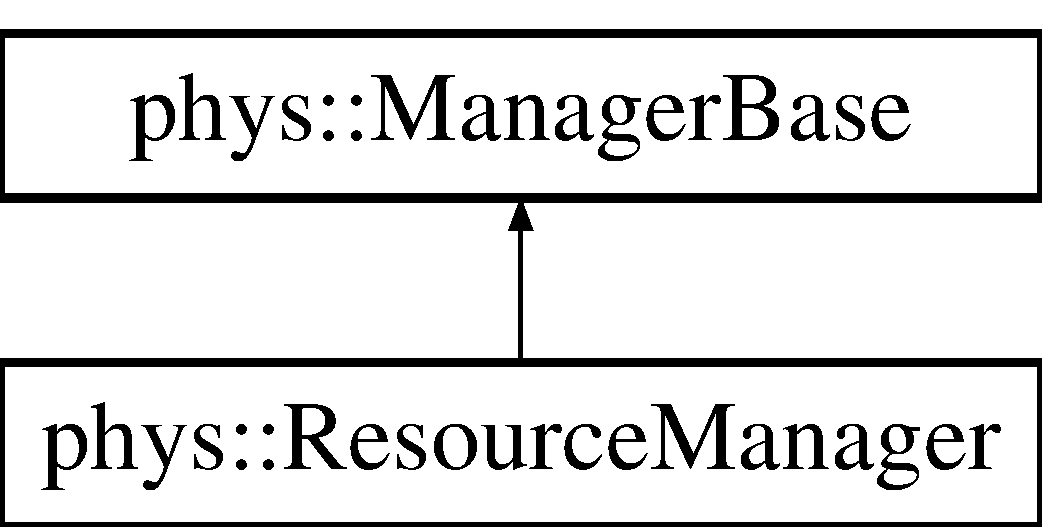
\includegraphics[height=2.000000cm]{d1/d35/classphys_1_1ResourceManager}
\end{center}
\end{figure}
\subsubsection*{Public Member Functions}
\begin{DoxyCompactItemize}
\item 
\hyperlink{classphys_1_1ResourceManager_af114d84fa357432db4184bfd322495b6}{ResourceManager} ()
\begin{DoxyCompactList}\small\item\em Class constructor. \item\end{DoxyCompactList}\item 
\hyperlink{classphys_1_1ResourceManager_a426d4d684a9ecf98359362243ce01072}{$\sim$ResourceManager} ()
\item 
bool \hyperlink{classphys_1_1ResourceManager_a9511ec29e5c732602b1495173abf56ef}{ExportShapeData} (\hyperlink{classphys_1_1ActorBase}{ActorBase} $\ast$Actor, const \hyperlink{namespacephys_aa03900411993de7fbfec4789bc1d392e}{String} \&FileName)
\begin{DoxyCompactList}\small\item\em Exports an actors shape data to a file. \item\end{DoxyCompactList}\item 
bool \hyperlink{classphys_1_1ResourceManager_a6fb3434f5d7be221e7a474765c625ad9}{ImportShapeData} (\hyperlink{classphys_1_1ActorBase}{ActorBase} $\ast$Actor, const \hyperlink{namespacephys_aa03900411993de7fbfec4789bc1d392e}{String} \&FileName)
\begin{DoxyCompactList}\small\item\em Imports serialized shape data from the disk to be used in an Actor. \item\end{DoxyCompactList}\item 
void \hyperlink{classphys_1_1ResourceManager_a0d7d3adce2ad4c70a3e867396e17b090}{AddResourceLocation} (const \hyperlink{namespacephys_aa03900411993de7fbfec4789bc1d392e}{String} \&Location, const \hyperlink{namespacephys_aa03900411993de7fbfec4789bc1d392e}{String} \&Type, const \hyperlink{namespacephys_aa03900411993de7fbfec4789bc1d392e}{String} \&Group, const bool \&recursive=false)
\begin{DoxyCompactList}\small\item\em Adds a location for graphical resources. \item\end{DoxyCompactList}\item 
void \hyperlink{classphys_1_1ResourceManager_a6ac7835a02dff32e60a73320f9c9dabb}{DeclareResource} (const \hyperlink{namespacephys_aa03900411993de7fbfec4789bc1d392e}{String} \&Name, const \hyperlink{namespacephys_aa03900411993de7fbfec4789bc1d392e}{String} \&Type, const \hyperlink{namespacephys_aa03900411993de7fbfec4789bc1d392e}{String} \&Group)
\begin{DoxyCompactList}\small\item\em Prepares the resource for use. \item\end{DoxyCompactList}\item 
void \hyperlink{classphys_1_1ResourceManager_aa2f44129dfc3dc0b0ee332a2bba6078d}{InitResourceGroup} (const \hyperlink{namespacephys_aa03900411993de7fbfec4789bc1d392e}{String} \&Name)
\begin{DoxyCompactList}\small\item\em Makes a resource group ready to use. \item\end{DoxyCompactList}\item 
\hypertarget{classphys_1_1ResourceManager_a348f333ffd9638decd144bf9d65ca05d}{
void \hyperlink{classphys_1_1ResourceManager_a348f333ffd9638decd144bf9d65ca05d}{ParseMaterialScripts} ()}
\label{d1/d35/classphys_1_1ResourceManager_a348f333ffd9638decd144bf9d65ca05d}

\begin{DoxyCompactList}\small\item\em Parses all Ogre Material scripts. \item\end{DoxyCompactList}\item 
\hyperlink{classphys_1_1ResourceInputStream}{ResourceInputStream} $\ast$ \hyperlink{classphys_1_1ResourceManager_a13f0aef080b9a353fe6c910c2781de50}{GetResourceStream} (const \hyperlink{namespacephys_aa03900411993de7fbfec4789bc1d392e}{String} \&FileName)
\begin{DoxyCompactList}\small\item\em Get a stream to read from the specified file. \item\end{DoxyCompactList}\item 
void \hyperlink{classphys_1_1ResourceManager_a9be3250f1f1153c9e079f82736eb00a8}{Initialize} ()
\begin{DoxyCompactList}\small\item\em Empty Initializor. \item\end{DoxyCompactList}\item 
void \hyperlink{classphys_1_1ResourceManager_a2114714999441c095bc28d3673c2490e}{DoMainLoopItems} ()
\begin{DoxyCompactList}\small\item\em Empty MainLoopItems. \item\end{DoxyCompactList}\item 
\hyperlink{classphys_1_1ManagerBase_aaa6ccddf23892eaccb898529414f80a5}{ManagerBase::ManagerTypeName} \hyperlink{classphys_1_1ResourceManager_a9e5468e5428f5c108c7b3c01e94eba46}{GetType} () const 
\begin{DoxyCompactList}\small\item\em This returns the type of this manager. \item\end{DoxyCompactList}\end{DoxyCompactItemize}
\subsubsection*{Protected Member Functions}
\begin{DoxyCompactItemize}
\item 
\hypertarget{classphys_1_1ResourceManager_a1823d2d08fc3b6052ed893896eef6291}{
void \hyperlink{classphys_1_1ResourceManager_a1823d2d08fc3b6052ed893896eef6291}{ApplyShapeToActor} (\hyperlink{classphys_1_1ActorBase}{ActorBase} $\ast$Actor, btCollisionShape $\ast$ColShape)}
\label{d1/d35/classphys_1_1ResourceManager_a1823d2d08fc3b6052ed893896eef6291}

\begin{DoxyCompactList}\small\item\em Applies a saved shape to an Actor. \item\end{DoxyCompactList}\item 
\hypertarget{classphys_1_1ResourceManager_a7c84034fc45e64fc3a07f736230afd38}{
void {\bfseries AddResourceGroupName} (\hyperlink{namespacephys_aa03900411993de7fbfec4789bc1d392e}{String} Name)}
\label{d1/d35/classphys_1_1ResourceManager_a7c84034fc45e64fc3a07f736230afd38}

\end{DoxyCompactItemize}
\subsubsection*{Protected Attributes}
\begin{DoxyCompactItemize}
\item 
\hypertarget{classphys_1_1ResourceManager_af19bf0549a0896cf84696a39f4ca817d}{
Ogre::ResourceGroupManager $\ast$ \hyperlink{classphys_1_1ResourceManager_af19bf0549a0896cf84696a39f4ca817d}{OgreResource}}
\label{d1/d35/classphys_1_1ResourceManager_af19bf0549a0896cf84696a39f4ca817d}

\begin{DoxyCompactList}\small\item\em Encapsulates the functionality of the ogre resource group manager. \item\end{DoxyCompactList}\item 
\hypertarget{classphys_1_1ResourceManager_a03a283e02f3639f5c1f2de915ed798ae}{
std::vector$<$ \hyperlink{classphys_1_1ResourceInputStream}{ResourceInputStream} $\ast$ $>$ \hyperlink{classphys_1_1ResourceManager_a03a283e02f3639f5c1f2de915ed798ae}{DeleteList}}
\label{d1/d35/classphys_1_1ResourceManager_a03a283e02f3639f5c1f2de915ed798ae}

\begin{DoxyCompactList}\small\item\em A list of Pointers to streams created to delete periodically. \item\end{DoxyCompactList}\item 
\hypertarget{classphys_1_1ResourceManager_a284bc8b042fffbb607355f7874692b54}{
std::vector$<$ \hyperlink{namespacephys_aa03900411993de7fbfec4789bc1d392e}{String} $>$ {\bfseries ResourceGroups}}
\label{d1/d35/classphys_1_1ResourceManager_a284bc8b042fffbb607355f7874692b54}

\end{DoxyCompactItemize}


\subsubsection{Detailed Description}
This is the manager responsible for the loading and unloading of files. This class is responsible for the reading and writing of files of all kinds, be it graphical meshes, physics data, or XMl files. 

Definition at line 68 of file resourcemanager.h.



\subsubsection{Constructor \& Destructor Documentation}
\hypertarget{classphys_1_1ResourceManager_af114d84fa357432db4184bfd322495b6}{
\index{phys::ResourceManager@{phys::ResourceManager}!ResourceManager@{ResourceManager}}
\index{ResourceManager@{ResourceManager}!phys::ResourceManager@{phys::ResourceManager}}
\paragraph[{ResourceManager}]{\setlength{\rightskip}{0pt plus 5cm}phys::ResourceManager::ResourceManager (
\begin{DoxyParamCaption}
{}
\end{DoxyParamCaption}
)}\hfill}
\label{d1/d35/classphys_1_1ResourceManager_af114d84fa357432db4184bfd322495b6}


Class constructor. 

Standard manager constructor. 

Definition at line 61 of file resourcemanager.cpp.

\hypertarget{classphys_1_1ResourceManager_a426d4d684a9ecf98359362243ce01072}{
\index{phys::ResourceManager@{phys::ResourceManager}!$\sim$ResourceManager@{$\sim$ResourceManager}}
\index{$\sim$ResourceManager@{$\sim$ResourceManager}!phys::ResourceManager@{phys::ResourceManager}}
\paragraph[{$\sim$ResourceManager}]{\setlength{\rightskip}{0pt plus 5cm}phys::ResourceManager::$\sim$ResourceManager (
\begin{DoxyParamCaption}
{}
\end{DoxyParamCaption}
)}\hfill}
\label{d1/d35/classphys_1_1ResourceManager_a426d4d684a9ecf98359362243ce01072}
Class Destructor. 

Definition at line 68 of file resourcemanager.cpp.



\subsubsection{Member Function Documentation}
\hypertarget{classphys_1_1ResourceManager_a0d7d3adce2ad4c70a3e867396e17b090}{
\index{phys::ResourceManager@{phys::ResourceManager}!AddResourceLocation@{AddResourceLocation}}
\index{AddResourceLocation@{AddResourceLocation}!phys::ResourceManager@{phys::ResourceManager}}
\paragraph[{AddResourceLocation}]{\setlength{\rightskip}{0pt plus 5cm}void phys::ResourceManager::AddResourceLocation (
\begin{DoxyParamCaption}
\item[{const {\bf String} \&}]{ Location, }
\item[{const {\bf String} \&}]{ Type, }
\item[{const {\bf String} \&}]{ Group, }
\item[{const bool \&}]{ recursive = {\ttfamily false}}
\end{DoxyParamCaption}
)}\hfill}
\label{d1/d35/classphys_1_1ResourceManager_a0d7d3adce2ad4c70a3e867396e17b090}


Adds a location for graphical resources. 

This function will add a location on the disk to find files needed to create and manipulate graphical objects. Once a resource is added it must be initalized using ResourceManager::InitResourceGroup(String Group). 
\begin{DoxyParams}{Parameters}
\item[{\em Location}]The location on the file system the resource can be found. \item[{\em Type}]The kind of file system the location can be found in. \par
 Options are: filesystem, zip. \item[{\em Group}]The name of the group the resources at this location belong to. \item[{\em recursive}]Whether or not to search sub-\/directories. \end{DoxyParams}


Definition at line 168 of file resourcemanager.cpp.

\hypertarget{classphys_1_1ResourceManager_a6ac7835a02dff32e60a73320f9c9dabb}{
\index{phys::ResourceManager@{phys::ResourceManager}!DeclareResource@{DeclareResource}}
\index{DeclareResource@{DeclareResource}!phys::ResourceManager@{phys::ResourceManager}}
\paragraph[{DeclareResource}]{\setlength{\rightskip}{0pt plus 5cm}void phys::ResourceManager::DeclareResource (
\begin{DoxyParamCaption}
\item[{const {\bf String} \&}]{ Name, }
\item[{const {\bf String} \&}]{ Type, }
\item[{const {\bf String} \&}]{ Group}
\end{DoxyParamCaption}
)}\hfill}
\label{d1/d35/classphys_1_1ResourceManager_a6ac7835a02dff32e60a73320f9c9dabb}


Prepares the resource for use. 

This function can be thought of as a preloader. This will prepare the defined resource located on the disk for use. 
\begin{DoxyParams}{Parameters}
\item[{\em Name}]Name of the file/resource to be 'prepared'. \item[{\em Type}]The type of resource that the file is. \par
 Options are: Font, GpuProgram, HighLevelGpuProgram, Material, Mesh, Skeleton, Texture. \item[{\em Group}]Name of the group the resource belongs to. \end{DoxyParams}


Definition at line 174 of file resourcemanager.cpp.

\hypertarget{classphys_1_1ResourceManager_a2114714999441c095bc28d3673c2490e}{
\index{phys::ResourceManager@{phys::ResourceManager}!DoMainLoopItems@{DoMainLoopItems}}
\index{DoMainLoopItems@{DoMainLoopItems}!phys::ResourceManager@{phys::ResourceManager}}
\paragraph[{DoMainLoopItems}]{\setlength{\rightskip}{0pt plus 5cm}void phys::ResourceManager::DoMainLoopItems (
\begin{DoxyParamCaption}
{}
\end{DoxyParamCaption}
)\hspace{0.3cm}{\ttfamily  \mbox{[}virtual\mbox{]}}}\hfill}
\label{d1/d35/classphys_1_1ResourceManager_a2114714999441c095bc28d3673c2490e}


Empty MainLoopItems. 

This class implements this for the sake of entension and compatibility this function does nothing. This is just empty during this round of refactoring, and this will get all the functionality that currently should be here, but is in the world. 

Implements \hyperlink{classphys_1_1ManagerBase_aa9e13a3f7c398b708f0f242610b5abf7}{phys::ManagerBase}.



Definition at line 215 of file resourcemanager.cpp.

\hypertarget{classphys_1_1ResourceManager_a9511ec29e5c732602b1495173abf56ef}{
\index{phys::ResourceManager@{phys::ResourceManager}!ExportShapeData@{ExportShapeData}}
\index{ExportShapeData@{ExportShapeData}!phys::ResourceManager@{phys::ResourceManager}}
\paragraph[{ExportShapeData}]{\setlength{\rightskip}{0pt plus 5cm}bool phys::ResourceManager::ExportShapeData (
\begin{DoxyParamCaption}
\item[{{\bf ActorBase} $\ast$}]{ Actor, }
\item[{const {\bf String} \&}]{ FileName}
\end{DoxyParamCaption}
)}\hfill}
\label{d1/d35/classphys_1_1ResourceManager_a9511ec29e5c732602b1495173abf56ef}


Exports an actors shape data to a file. 


\begin{DoxyParams}{Parameters}
\item[{\em FileName}]The Filename to save the data too. Remember to include a \char`\"{}.bullet\char`\"{} extension to the filename when serializing. \item[{\em Actor}]The Actor's Shape to save \end{DoxyParams}


Definition at line 106 of file resourcemanager.cpp.

\hypertarget{classphys_1_1ResourceManager_a13f0aef080b9a353fe6c910c2781de50}{
\index{phys::ResourceManager@{phys::ResourceManager}!GetResourceStream@{GetResourceStream}}
\index{GetResourceStream@{GetResourceStream}!phys::ResourceManager@{phys::ResourceManager}}
\paragraph[{GetResourceStream}]{\setlength{\rightskip}{0pt plus 5cm}{\bf ResourceInputStream} $\ast$ phys::ResourceManager::GetResourceStream (
\begin{DoxyParamCaption}
\item[{const {\bf String} \&}]{ FileName}
\end{DoxyParamCaption}
)}\hfill}
\label{d1/d35/classphys_1_1ResourceManager_a13f0aef080b9a353fe6c910c2781de50}


Get a stream to read from the specified file. 


\begin{DoxyParams}{Parameters}
\item[{\em FileName}]The name of the File you want to stream data from \end{DoxyParams}
\begin{DoxyReturn}{Returns}
An derivative of std::istream a \hyperlink{classphys_1_1ResourceInputStream}{ResourceInputStream} that will pull it's data from the desired resource
\end{DoxyReturn}
The returned \hyperlink{classphys_1_1ResourceInputStream}{ResourceInputStream} is the Caller's responsibility to deal with. If it is not deleted it is a memory leak. 

Definition at line 197 of file resourcemanager.cpp.

\hypertarget{classphys_1_1ResourceManager_a9e5468e5428f5c108c7b3c01e94eba46}{
\index{phys::ResourceManager@{phys::ResourceManager}!GetType@{GetType}}
\index{GetType@{GetType}!phys::ResourceManager@{phys::ResourceManager}}
\paragraph[{GetType}]{\setlength{\rightskip}{0pt plus 5cm}{\bf ManagerBase::ManagerTypeName} phys::ResourceManager::GetType (
\begin{DoxyParamCaption}
{}
\end{DoxyParamCaption}
) const\hspace{0.3cm}{\ttfamily  \mbox{[}virtual\mbox{]}}}\hfill}
\label{d1/d35/classphys_1_1ResourceManager_a9e5468e5428f5c108c7b3c01e94eba46}


This returns the type of this manager. 

\begin{DoxyReturn}{Returns}
This returns ManagerTypeName::ResourceManager 
\end{DoxyReturn}


Implements \hyperlink{classphys_1_1ManagerBase_aff400b6599db635e24796d8221e9a0e3}{phys::ManagerBase}.



Definition at line 219 of file resourcemanager.cpp.

\hypertarget{classphys_1_1ResourceManager_a6fb3434f5d7be221e7a474765c625ad9}{
\index{phys::ResourceManager@{phys::ResourceManager}!ImportShapeData@{ImportShapeData}}
\index{ImportShapeData@{ImportShapeData}!phys::ResourceManager@{phys::ResourceManager}}
\paragraph[{ImportShapeData}]{\setlength{\rightskip}{0pt plus 5cm}bool phys::ResourceManager::ImportShapeData (
\begin{DoxyParamCaption}
\item[{{\bf ActorBase} $\ast$}]{ Actor, }
\item[{const {\bf String} \&}]{ FileName}
\end{DoxyParamCaption}
)}\hfill}
\label{d1/d35/classphys_1_1ResourceManager_a6fb3434f5d7be221e7a474765c625ad9}


Imports serialized shape data from the disk to be used in an Actor. 


\begin{DoxyParams}{Parameters}
\item[{\em FileName}]The Filename to load the data from. Remember to include a \char`\"{}.bullet\char`\"{} extension to the filename when serializing. \item[{\em Actor}]The Actor's Shape to restore from file \end{DoxyParams}


Definition at line 126 of file resourcemanager.cpp.

\hypertarget{classphys_1_1ResourceManager_a9be3250f1f1153c9e079f82736eb00a8}{
\index{phys::ResourceManager@{phys::ResourceManager}!Initialize@{Initialize}}
\index{Initialize@{Initialize}!phys::ResourceManager@{phys::ResourceManager}}
\paragraph[{Initialize}]{\setlength{\rightskip}{0pt plus 5cm}void phys::ResourceManager::Initialize (
\begin{DoxyParamCaption}
{}
\end{DoxyParamCaption}
)\hspace{0.3cm}{\ttfamily  \mbox{[}virtual\mbox{]}}}\hfill}
\label{d1/d35/classphys_1_1ResourceManager_a9be3250f1f1153c9e079f82736eb00a8}


Empty Initializor. 

Functions inherited from \hyperlink{classphys_1_1ManagerBase}{ManagerBase}

This specific initializor is unneeded, but we implement it for compatibility. It also exists in case a derived class wants to override it for some reason. 

Implements \hyperlink{classphys_1_1ManagerBase_a57dd8e54e767427d5bdcc86dc66d73ed}{phys::ManagerBase}.



Definition at line 211 of file resourcemanager.cpp.

\hypertarget{classphys_1_1ResourceManager_aa2f44129dfc3dc0b0ee332a2bba6078d}{
\index{phys::ResourceManager@{phys::ResourceManager}!InitResourceGroup@{InitResourceGroup}}
\index{InitResourceGroup@{InitResourceGroup}!phys::ResourceManager@{phys::ResourceManager}}
\paragraph[{InitResourceGroup}]{\setlength{\rightskip}{0pt plus 5cm}void phys::ResourceManager::InitResourceGroup (
\begin{DoxyParamCaption}
\item[{const {\bf String} \&}]{ Name}
\end{DoxyParamCaption}
)}\hfill}
\label{d1/d35/classphys_1_1ResourceManager_aa2f44129dfc3dc0b0ee332a2bba6078d}


Makes a resource group ready to use. 

After adding all of your resources and declaring them as nessessary, this function is the final step. After calling this function any and all resources within the defined group will be ready to use. Do not initialize any more groups then you need to however, as that will take up memory and drop performance. 
\begin{DoxyParams}{Parameters}
\item[{\em Name}]Name of the resource group. \end{DoxyParams}


Definition at line 179 of file resourcemanager.cpp.



The documentation for this class was generated from the following files:\begin{DoxyCompactItemize}
\item 
resourcemanager.h\item 
resourcemanager.cpp\end{DoxyCompactItemize}

\hypertarget{classphys_1_1SceneManager}{
\subsection{phys::SceneManager Class Reference}
\label{dd/da8/classphys_1_1SceneManager}\index{phys::SceneManager@{phys::SceneManager}}
}


This class contains utilities and functions to allow the manipulation of the Graphical scene, rather then the physics inside, or the object inside.  




{\ttfamily \#include $<$scenemanager.h$>$}

Inheritance diagram for phys::SceneManager:\begin{figure}[H]
\begin{center}
\leavevmode
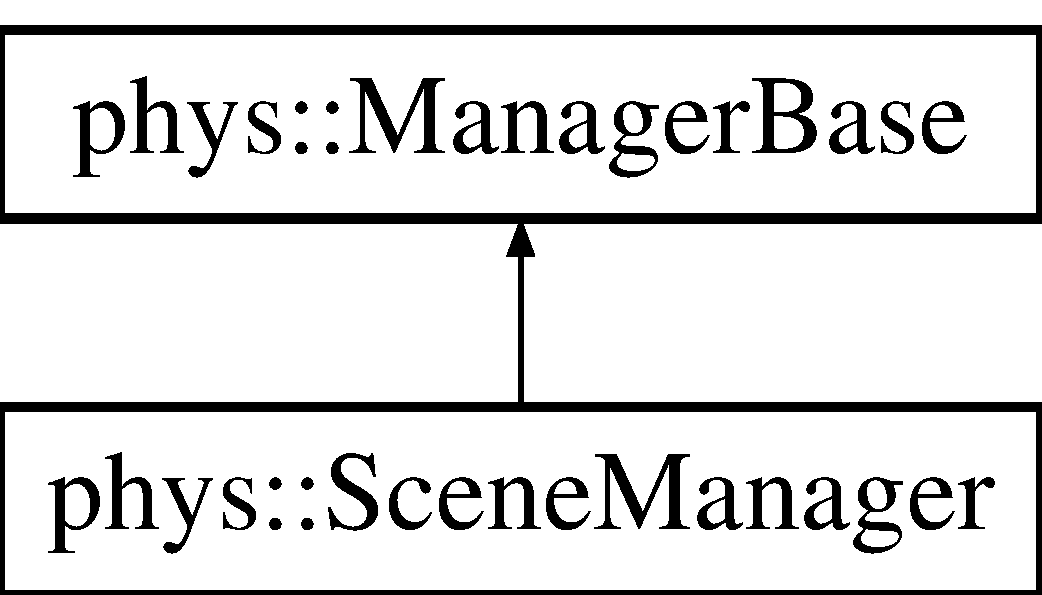
\includegraphics[height=2.000000cm]{dd/da8/classphys_1_1SceneManager}
\end{center}
\end{figure}
\subsubsection*{Public Types}
\begin{DoxyCompactItemize}
\item 
enum \hyperlink{classphys_1_1SceneManager_a14fe15dcf41564fdf12f3e11c1a4b774}{SceneManagerType} \{ \hyperlink{classphys_1_1SceneManager_a14fe15dcf41564fdf12f3e11c1a4b774ae556c6d77cbc80f7fddb859d1bde7738}{Generic} =  0, 
\hyperlink{classphys_1_1SceneManager_a14fe15dcf41564fdf12f3e11c1a4b774a76452baaacf89eac4d34596826d19ca7}{Exterior} =  1, 
\hyperlink{classphys_1_1SceneManager_a14fe15dcf41564fdf12f3e11c1a4b774a483ff734e11e4f63eb81569b2ade26e1}{ExteriorRealFar} =  2, 
\hyperlink{classphys_1_1SceneManager_a14fe15dcf41564fdf12f3e11c1a4b774ab582df9aaf3ba748a7dd4c6f5bd7250d}{Interior} =  3
 \}
\begin{DoxyCompactList}\small\item\em Needs to be documented. \item\end{DoxyCompactList}\item 
enum \hyperlink{classphys_1_1SceneManager_a427f1bbb52c11ad07352ae01d8b3c746}{SceneShadowTechnique} \{ \par
\hyperlink{classphys_1_1SceneManager_a427f1bbb52c11ad07352ae01d8b3c746ad96e23ac363ae9de73e2d3816ae66f2e}{SST\_\-None} =  0, 
\hyperlink{classphys_1_1SceneManager_a427f1bbb52c11ad07352ae01d8b3c746a9b11aebab7ffc5ff359f5a49b4ff5e7d}{SST\_\-Stencil\_\-Modulative} =  1, 
\hyperlink{classphys_1_1SceneManager_a427f1bbb52c11ad07352ae01d8b3c746a17ba96aa6b125ac6c787851815370d97}{SST\_\-Stencil\_\-Additive} =  2, 
\hyperlink{classphys_1_1SceneManager_a427f1bbb52c11ad07352ae01d8b3c746a6ce2d2624df59f6c2fb6f3cb07d3adf8}{SST\_\-Texture\_\-Modulative} =  11, 
\par
\hyperlink{classphys_1_1SceneManager_a427f1bbb52c11ad07352ae01d8b3c746af9aba631cfa4181d30d83fa8c2bd71de}{SST\_\-Texture\_\-Additive} =  12, 
\hyperlink{classphys_1_1SceneManager_a427f1bbb52c11ad07352ae01d8b3c746a2cb2c18049fd6f062db3a25e45aa9a16}{SST\_\-Texture\_\-Additive\_\-Integrated} =  13, 
\hyperlink{classphys_1_1SceneManager_a427f1bbb52c11ad07352ae01d8b3c746a85419a12cb66f84865d9c0e50503af8c}{SST\_\-Texture\_\-Modulative\_\-Integrated} =  14
 \}
\begin{DoxyCompactList}\small\item\em needs to be documented \item\end{DoxyCompactList}\item 
enum \hyperlink{classphys_1_1SceneManager_a91dd086aabaab926d070c65fc14828d6}{SkyMethod} \{ \hyperlink{classphys_1_1SceneManager_a91dd086aabaab926d070c65fc14828d6a11aa0789aa0b39732c6968587b56e026}{SkyNone} =  0, 
\hyperlink{classphys_1_1SceneManager_a91dd086aabaab926d070c65fc14828d6af1251fd4f24ec8061fb585474635c10f}{SkyPlane} =  1, 
\hyperlink{classphys_1_1SceneManager_a91dd086aabaab926d070c65fc14828d6ac2ecb3ad06b3b545c27b7d70ca1b3a5a}{SkyBox} =  2, 
\hyperlink{classphys_1_1SceneManager_a91dd086aabaab926d070c65fc14828d6aa3c39672f84de2ae8ffb883e04af2edd}{SkyDome} =  3
 \}
\begin{DoxyCompactList}\small\item\em Used to help identify which method is used to draw the sky, if any. \item\end{DoxyCompactList}\item 
\hypertarget{classphys_1_1SceneManager_a2764b9082b4aecbf833c2f6e9f174ba0}{
typedef std::vector$<$ \hyperlink{classphys_1_1Light}{Light} $\ast$ $>$::iterator \hyperlink{classphys_1_1SceneManager_a2764b9082b4aecbf833c2f6e9f174ba0}{LightIterator}}
\label{dd/da8/classphys_1_1SceneManager_a2764b9082b4aecbf833c2f6e9f174ba0}

\begin{DoxyCompactList}\small\item\em Used to make working with the Lights easier. \item\end{DoxyCompactList}\item 
\hypertarget{classphys_1_1SceneManager_a417c57b560317661d0c7d836a88f52ac}{
typedef std::vector$<$ \hyperlink{classphys_1_1Light}{Light} $\ast$ $>$::const\_\-iterator \hyperlink{classphys_1_1SceneManager_a417c57b560317661d0c7d836a88f52ac}{ConstLightIterator}}
\label{dd/da8/classphys_1_1SceneManager_a417c57b560317661d0c7d836a88f52ac}

\begin{DoxyCompactList}\small\item\em Used to make working with the Lights easier, and avoid the risk of accidentally changing them. \item\end{DoxyCompactList}\item 
\hypertarget{classphys_1_1SceneManager_a668ef8db2053cc15cc48b21fa6240c3e}{
typedef std::vector$<$ \hyperlink{classphys_1_1ParticleEffect}{ParticleEffect} $\ast$ $>$::iterator \hyperlink{classphys_1_1SceneManager_a668ef8db2053cc15cc48b21fa6240c3e}{ParticleEffectIterator}}
\label{dd/da8/classphys_1_1SceneManager_a668ef8db2053cc15cc48b21fa6240c3e}

\begin{DoxyCompactList}\small\item\em Used to make working with the Lights easier. \item\end{DoxyCompactList}\item 
\hypertarget{classphys_1_1SceneManager_a0026f62b121b0d7010a67a79fdc9000c}{
typedef std::vector$<$ \hyperlink{classphys_1_1ParticleEffect}{ParticleEffect} $\ast$ $>$::const\_\-iterator \hyperlink{classphys_1_1SceneManager_a0026f62b121b0d7010a67a79fdc9000c}{ConstParticleEffectIterator}}
\label{dd/da8/classphys_1_1SceneManager_a0026f62b121b0d7010a67a79fdc9000c}

\begin{DoxyCompactList}\small\item\em Used to make working with the Lights easier, and avoid the risk of accidentally changing them. \item\end{DoxyCompactList}\item 
\hypertarget{classphys_1_1SceneManager_a67b62f6e9116423306b82e20cb2415fd}{
typedef std::vector$<$ \hyperlink{classphys_1_1WorldNode}{WorldNode} $\ast$ $>$::iterator \hyperlink{classphys_1_1SceneManager_a67b62f6e9116423306b82e20cb2415fd}{WorldNodeIterator}}
\label{dd/da8/classphys_1_1SceneManager_a67b62f6e9116423306b82e20cb2415fd}

\begin{DoxyCompactList}\small\item\em Used to make working with the Lights easier. \item\end{DoxyCompactList}\item 
\hypertarget{classphys_1_1SceneManager_aa893eadb43492c0a4a9cafe2d150742c}{
typedef std::vector$<$ \hyperlink{classphys_1_1WorldNode}{WorldNode} $\ast$ $>$::const\_\-iterator \hyperlink{classphys_1_1SceneManager_aa893eadb43492c0a4a9cafe2d150742c}{ConstWorldNodeIterator}}
\label{dd/da8/classphys_1_1SceneManager_aa893eadb43492c0a4a9cafe2d150742c}

\begin{DoxyCompactList}\small\item\em Used to make working with the Lights easier, and avoid the risk of accidentally changing them. \item\end{DoxyCompactList}\end{DoxyCompactItemize}
\subsubsection*{Public Member Functions}
\begin{DoxyCompactItemize}
\item 
\hyperlink{classphys_1_1SceneManager_a6a6a5b747704d3f4bb724f1b893e2695}{SceneManager} (\hyperlink{classphys_1_1SceneManager_a14fe15dcf41564fdf12f3e11c1a4b774}{SceneManager::SceneManagerType} ManagerType)
\begin{DoxyCompactList}\small\item\em Class Constructor. \item\end{DoxyCompactList}\item 
\hyperlink{classphys_1_1SceneManager_a5076643eec92dc0c9c9ccb7ac2225cde}{$\sim$SceneManager} ()
\begin{DoxyCompactList}\small\item\em Class Destructor. \item\end{DoxyCompactList}\item 
void \hyperlink{classphys_1_1SceneManager_a620405e97c1ff656dc09524e4c1d1b4b}{SetSceneShadowTechnique} (\hyperlink{classphys_1_1SceneManager_a427f1bbb52c11ad07352ae01d8b3c746}{SceneShadowTechnique} Shadows)
\begin{DoxyCompactList}\small\item\em Sets the type of shadows to be used when rendering the scene. \item\end{DoxyCompactList}\item 
\hyperlink{classphys_1_1SceneManager_a427f1bbb52c11ad07352ae01d8b3c746}{SceneShadowTechnique} \hyperlink{classphys_1_1SceneManager_a29cb7b20fb3b64b95bd951d65ffe8bca}{GetSceneShadowTechnique} () const 
\begin{DoxyCompactList}\small\item\em Gets the currently set shadow technique. \item\end{DoxyCompactList}\item 
void \hyperlink{classphys_1_1SceneManager_a6e09079b87f29fd3c7b7716f88d5081f}{SetShadowTextureCount} (const \hyperlink{namespacephys_a460f6bc24c8dd347b05e0366ae34f34a}{Whole} \&Count)
\begin{DoxyCompactList}\small\item\em Sets the number of textures to be alloted for creating shadows. \item\end{DoxyCompactList}\item 
\hyperlink{namespacephys_a460f6bc24c8dd347b05e0366ae34f34a}{Whole} \hyperlink{classphys_1_1SceneManager_ac5b37e84f72853b4705f164919e2daa3}{GetShadowTextureCount} () const 
\begin{DoxyCompactList}\small\item\em Gets the currently set number of textures being used to make texture shadows. \item\end{DoxyCompactList}\item 
void \hyperlink{classphys_1_1SceneManager_ab7022066631b9871f8d6e4da6aaa45ed}{SetShadowTextureSize} (unsigned short Size)
\begin{DoxyCompactList}\small\item\em Sets the size of all texture based shadows. \item\end{DoxyCompactList}\item 
unsigned short \hyperlink{classphys_1_1SceneManager_a0ed48ad404c48c492130f8f3f5eb2b26}{GetShadowTextureSize} () const 
\begin{DoxyCompactList}\small\item\em Retrieve the size of textures. \item\end{DoxyCompactList}\item 
void \hyperlink{classphys_1_1SceneManager_a124396e75cc26b400f08474a124b3fb3}{SetShadowFarDistance} (const \hyperlink{namespacephys_af7eb897198d265b8e868f45240230d5f}{Real} \&FarDist)
\begin{DoxyCompactList}\small\item\em Sets the maximum distance from the camera that shadows will be visible. \item\end{DoxyCompactList}\item 
\hyperlink{namespacephys_af7eb897198d265b8e868f45240230d5f}{Real} \hyperlink{classphys_1_1SceneManager_a496228d09b1ee83a6d476565cc334f3b}{GetShadowFarDistance} () const 
\begin{DoxyCompactList}\small\item\em Gets the maximum distance from the camera that shadows will be visible. \item\end{DoxyCompactList}\item 
void \hyperlink{classphys_1_1SceneManager_a5fae70a91407ed773541025f93c52342}{SetShadowColour} (const \hyperlink{classphys_1_1ColourValue}{ColourValue} \&ShadowColour)
\begin{DoxyCompactList}\small\item\em Sets the colour to be used when casting shadows. \item\end{DoxyCompactList}\item 
\hyperlink{classphys_1_1ColourValue}{ColourValue} \hyperlink{classphys_1_1SceneManager_ab008f05d80ca7e8fa7df3ab4e621173f}{GetShadowColour} () const 
\begin{DoxyCompactList}\small\item\em Gets the colour being used when casting shadows. \item\end{DoxyCompactList}\item 
void \hyperlink{classphys_1_1SceneManager_a5593ec052782189f77ef27a10272da8f}{CreateSkyPlane} (const \hyperlink{classphys_1_1Plane}{Plane} \&SkyPlane\_\-, const \hyperlink{namespacephys_aa03900411993de7fbfec4789bc1d392e}{String} \&Material, const \hyperlink{namespacephys_aa03900411993de7fbfec4789bc1d392e}{String} \&Group, \hyperlink{namespacephys_af7eb897198d265b8e868f45240230d5f}{Real} Scale=1000.0, \hyperlink{namespacephys_af7eb897198d265b8e868f45240230d5f}{Real} Tiling=10.0, bool DrawFirst=true, \hyperlink{namespacephys_af7eb897198d265b8e868f45240230d5f}{Real} Bow=0, int XSegments=1, int YSegments=1)
\begin{DoxyCompactList}\small\item\em Creates a skyplane for use in making a sky. \item\end{DoxyCompactList}\item 
void \hyperlink{classphys_1_1SceneManager_af5763eedafdd11712b55ee33a11bd2b8}{DisableSkyPlane} ()
\begin{DoxyCompactList}\small\item\em Disables the currently active skyplane. \item\end{DoxyCompactList}\item 
void \hyperlink{classphys_1_1SceneManager_a24e2699227790a0431613e49f3b68db0}{CreateSkyBox} (const \hyperlink{namespacephys_aa03900411993de7fbfec4789bc1d392e}{String} \&Material, const \hyperlink{namespacephys_aa03900411993de7fbfec4789bc1d392e}{String} \&Group, \hyperlink{namespacephys_af7eb897198d265b8e868f45240230d5f}{Real} Distance, bool DrawFirst=true, \hyperlink{classphys_1_1Quaternion}{Quaternion} Orientation=\hyperlink{classphys_1_1Quaternion}{Quaternion}())
\begin{DoxyCompactList}\small\item\em Creates a skybox for use in making a sky. \item\end{DoxyCompactList}\item 
void \hyperlink{classphys_1_1SceneManager_acb9c87d510955f028db24ce49944a97a}{DisableSkyBox} ()
\begin{DoxyCompactList}\small\item\em Disables the currently active skybox. \item\end{DoxyCompactList}\item 
void \hyperlink{classphys_1_1SceneManager_a965bec06f491a619101c3142ca1eb47c}{CreateSkyDome} (const \hyperlink{namespacephys_aa03900411993de7fbfec4789bc1d392e}{String} \&Material, const \hyperlink{namespacephys_aa03900411993de7fbfec4789bc1d392e}{String} \&Group, \hyperlink{namespacephys_af7eb897198d265b8e868f45240230d5f}{Real} Distance, \hyperlink{namespacephys_af7eb897198d265b8e868f45240230d5f}{Real} Curvature=10.0, \hyperlink{namespacephys_af7eb897198d265b8e868f45240230d5f}{Real} Tiling=8.0, bool DrawFirst=true, \hyperlink{classphys_1_1Quaternion}{Quaternion} Orientation=\hyperlink{classphys_1_1Quaternion}{Quaternion}(), int XSegments=16, int YSegments=16)
\begin{DoxyCompactList}\small\item\em Creates a skydome for use in making a sky. \item\end{DoxyCompactList}\item 
void \hyperlink{classphys_1_1SceneManager_a11bf15ca8c7d758ee50e423ad03d2625}{DisableSkyDome} ()
\begin{DoxyCompactList}\small\item\em Disables the currently active skydome. \item\end{DoxyCompactList}\item 
\hypertarget{classphys_1_1SceneManager_a929da26f1fcdbe98484b7162dcf2d16f}{
void \hyperlink{classphys_1_1SceneManager_a929da26f1fcdbe98484b7162dcf2d16f}{DisableSky} ()}
\label{dd/da8/classphys_1_1SceneManager_a929da26f1fcdbe98484b7162dcf2d16f}

\begin{DoxyCompactList}\small\item\em If any sky is active, disable it. \item\end{DoxyCompactList}\item 
\hyperlink{classphys_1_1SceneManager_a91dd086aabaab926d070c65fc14828d6}{SkyMethod} \hyperlink{classphys_1_1SceneManager_a39155e9eaa52789884fcc54d93f8cf3a}{WhichSky} () const 
\begin{DoxyCompactList}\small\item\em get the kind of sy in use \item\end{DoxyCompactList}\item 
void \hyperlink{classphys_1_1SceneManager_a686b7199aff8db87af84f40ec933809a}{SetAmbientLight} (\hyperlink{namespacephys_af7eb897198d265b8e868f45240230d5f}{Real} Red=1.0, \hyperlink{namespacephys_af7eb897198d265b8e868f45240230d5f}{Real} Green=1.0, \hyperlink{namespacephys_af7eb897198d265b8e868f45240230d5f}{Real} Blue=1.0, \hyperlink{namespacephys_af7eb897198d265b8e868f45240230d5f}{Real} Alpha=1.0)
\begin{DoxyCompactList}\small\item\em Sets the ambient light for the scene. \item\end{DoxyCompactList}\item 
void \hyperlink{classphys_1_1SceneManager_af5af99740fefeb411caff8fd004b4103}{SetAmbientLight} (const \hyperlink{classphys_1_1ColourValue}{ColourValue} \&LightColor)
\begin{DoxyCompactList}\small\item\em Sets the ambient light for the scene, in a single value. \item\end{DoxyCompactList}\item 
\hyperlink{classphys_1_1ColourValue}{ColourValue} \hyperlink{classphys_1_1SceneManager_a4ab204cf9bdfe267561ba2710108c68f}{GetAmbientLight} () const 
\begin{DoxyCompactList}\small\item\em Retrieve the level of the ambient light. \item\end{DoxyCompactList}\item 
\hyperlink{classphys_1_1Light}{Light} $\ast$ \hyperlink{classphys_1_1SceneManager_aaf14df62a5d6c55c3307d154a0caf5ea}{CreateLight} (const \hyperlink{namespacephys_aa03900411993de7fbfec4789bc1d392e}{String} \&Name)
\begin{DoxyCompactList}\small\item\em Creates a dynamic light. \item\end{DoxyCompactList}\item 
\hyperlink{classphys_1_1Light}{Light} $\ast$ \hyperlink{classphys_1_1SceneManager_a00849466a4248d71f7e1ecfd5a07a89c}{GetLight} (const \hyperlink{namespacephys_aa03900411993de7fbfec4789bc1d392e}{String} \&Name) const 
\begin{DoxyCompactList}\small\item\em Gets an already created light by name. \item\end{DoxyCompactList}\item 
\hyperlink{classphys_1_1Light}{Light} $\ast$ \hyperlink{classphys_1_1SceneManager_a3c5aaeb80eed8032d6f9417073d2be8b}{GetLight} (\hyperlink{namespacephys_a460f6bc24c8dd347b05e0366ae34f34a}{Whole} Index) const 
\begin{DoxyCompactList}\small\item\em Gets an already created light by index. \item\end{DoxyCompactList}\item 
\hyperlink{namespacephys_a460f6bc24c8dd347b05e0366ae34f34a}{Whole} \hyperlink{classphys_1_1SceneManager_aa1eaa692e63a6d8e328d2f0e4a2f9bf8}{GetNumLights} () const 
\begin{DoxyCompactList}\small\item\em Gets the number of lights created and stored in this manager. \item\end{DoxyCompactList}\item 
void \hyperlink{classphys_1_1SceneManager_a0f6ebec4e8a372b0fcc2b2205bac7725}{DestroyLight} (\hyperlink{classphys_1_1Light}{Light} $\ast$light)
\begin{DoxyCompactList}\small\item\em Deletes a light and removes all trace of it from the manager. \item\end{DoxyCompactList}\item 
\hypertarget{classphys_1_1SceneManager_a6246fbc7c12300416dfc99bdbb22d002}{
void \hyperlink{classphys_1_1SceneManager_a6246fbc7c12300416dfc99bdbb22d002}{DestroyAllLights} ()}
\label{dd/da8/classphys_1_1SceneManager_a6246fbc7c12300416dfc99bdbb22d002}

\begin{DoxyCompactList}\small\item\em Destroys all lights currently in the manager. \item\end{DoxyCompactList}\item 
\hyperlink{classphys_1_1SceneManager_a2764b9082b4aecbf833c2f6e9f174ba0}{LightIterator} \hyperlink{classphys_1_1SceneManager_a710bed731b5674cae3bb09853f3a0cd1}{BeginLight} ()
\begin{DoxyCompactList}\small\item\em Get a LightIterator to the first Light$\ast$. \item\end{DoxyCompactList}\item 
\hyperlink{classphys_1_1SceneManager_a2764b9082b4aecbf833c2f6e9f174ba0}{LightIterator} \hyperlink{classphys_1_1SceneManager_a4b44838cddfa710a538c02f3b261c3c7}{EndLight} ()
\begin{DoxyCompactList}\small\item\em Get a LightIterator to one past the last Light$\ast$. \item\end{DoxyCompactList}\item 
\hyperlink{classphys_1_1SceneManager_a417c57b560317661d0c7d836a88f52ac}{ConstLightIterator} \hyperlink{classphys_1_1SceneManager_a468298df736ca62876592bf5e8ce36ac}{BeginLight} () const 
\begin{DoxyCompactList}\small\item\em Get a ConstLightIterator to one past the last Light$\ast$. \item\end{DoxyCompactList}\item 
\hyperlink{classphys_1_1SceneManager_a417c57b560317661d0c7d836a88f52ac}{ConstLightIterator} \hyperlink{classphys_1_1SceneManager_a606664d81c965a853dc1adf22c4559dc}{EndLight} () const 
\begin{DoxyCompactList}\small\item\em Get a ConstLightIterator to one past the last Light$\ast$. \item\end{DoxyCompactList}\item 
\hyperlink{classphys_1_1ParticleEffect}{ParticleEffect} $\ast$ \hyperlink{classphys_1_1SceneManager_a67a33ba38c8e8b198c52ca7bcf847751}{CreateParticleEffect} (const \hyperlink{namespacephys_aa03900411993de7fbfec4789bc1d392e}{String} \&Name, const \hyperlink{namespacephys_aa03900411993de7fbfec4789bc1d392e}{String} \&Template)
\begin{DoxyCompactList}\small\item\em Creates a particle effect. \item\end{DoxyCompactList}\item 
\hyperlink{classphys_1_1ParticleEffect}{ParticleEffect} $\ast$ \hyperlink{classphys_1_1SceneManager_af1f8d6b77b1088dea72685719ff6936f}{GetParticleEffect} (const \hyperlink{namespacephys_aa03900411993de7fbfec4789bc1d392e}{String} \&Name) const 
\begin{DoxyCompactList}\small\item\em Gets an already created particle effect by name. \item\end{DoxyCompactList}\item 
\hyperlink{classphys_1_1ParticleEffect}{ParticleEffect} $\ast$ \hyperlink{classphys_1_1SceneManager_acfe014153bbda04b181959774536aec5}{GetParticleEffect} (\hyperlink{namespacephys_a460f6bc24c8dd347b05e0366ae34f34a}{Whole} Index) const 
\begin{DoxyCompactList}\small\item\em Gets an already created particle effect by index. \item\end{DoxyCompactList}\item 
\hyperlink{namespacephys_a460f6bc24c8dd347b05e0366ae34f34a}{Whole} \hyperlink{classphys_1_1SceneManager_aad3e20c92eef52372671450704a2ac51}{GetNumParticleEffects} () const 
\begin{DoxyCompactList}\small\item\em Gets the number of particle effects created and stored in this manager. \item\end{DoxyCompactList}\item 
void \hyperlink{classphys_1_1SceneManager_addce8f82a6758db345568dbd4a88f5b9}{DestroyParticleEffect} (\hyperlink{classphys_1_1ParticleEffect}{ParticleEffect} $\ast$particleeffect)
\begin{DoxyCompactList}\small\item\em Deletes a particle effect and removes all trace of it from the manager. \item\end{DoxyCompactList}\item 
\hypertarget{classphys_1_1SceneManager_ac70441dd536d4b9be2c2143148b75420}{
void \hyperlink{classphys_1_1SceneManager_ac70441dd536d4b9be2c2143148b75420}{DestroyAllParticleEffects} ()}
\label{dd/da8/classphys_1_1SceneManager_ac70441dd536d4b9be2c2143148b75420}

\begin{DoxyCompactList}\small\item\em Destroys all particle effects currently in the manager. \item\end{DoxyCompactList}\item 
\hyperlink{classphys_1_1SceneManager_a668ef8db2053cc15cc48b21fa6240c3e}{ParticleEffectIterator} \hyperlink{classphys_1_1SceneManager_a603f8cbd672cf081f869af4392c8cb4b}{BeginParticleEffect} ()
\begin{DoxyCompactList}\small\item\em Get a ParticleEffectIterator to the first ParticleEffect$\ast$. \item\end{DoxyCompactList}\item 
\hyperlink{classphys_1_1SceneManager_a668ef8db2053cc15cc48b21fa6240c3e}{ParticleEffectIterator} \hyperlink{classphys_1_1SceneManager_acc2e73606de2ecd452a0231473bfc2e6}{EndParticleEffect} ()
\begin{DoxyCompactList}\small\item\em Get a ParticleEffectIterator to one past the last ParticleEffect$\ast$. \item\end{DoxyCompactList}\item 
\hyperlink{classphys_1_1SceneManager_a0026f62b121b0d7010a67a79fdc9000c}{ConstParticleEffectIterator} \hyperlink{classphys_1_1SceneManager_a2289b4e4a5c4a3bc63480a1b7bbd70f4}{BeginParticleEffect} () const 
\begin{DoxyCompactList}\small\item\em Get a ConstParticleEffectIterator to one past the last ParticleEffect$\ast$. \item\end{DoxyCompactList}\item 
\hyperlink{classphys_1_1SceneManager_a0026f62b121b0d7010a67a79fdc9000c}{ConstParticleEffectIterator} \hyperlink{classphys_1_1SceneManager_ac06259a883a3d380334fe9b097e859f3}{EndParticleEffect} () const 
\begin{DoxyCompactList}\small\item\em Get a ConstParticleEffectIterator to one past the last ParticleEffect$\ast$. \item\end{DoxyCompactList}\item 
\hyperlink{classphys_1_1WorldNode}{WorldNode} $\ast$ \hyperlink{classphys_1_1SceneManager_ad86be1c140e04c7579af80c1e33150fd}{CreateOrbitingNode} (const \hyperlink{namespacephys_aa03900411993de7fbfec4789bc1d392e}{String} \&Name, \hyperlink{classphys_1_1Vector3}{Vector3} Target, \hyperlink{classphys_1_1Vector3}{Vector3} RelativeLoc, bool AutoTrack)
\begin{DoxyCompactList}\small\item\em Creates a node that will orbit around a point. \item\end{DoxyCompactList}\item 
\hyperlink{classphys_1_1WorldNode}{WorldNode} $\ast$ \hyperlink{classphys_1_1SceneManager_afb93b25cdd669066481e7bc81c33674a}{CreateStandNode} (const \hyperlink{namespacephys_aa03900411993de7fbfec4789bc1d392e}{String} \&Name, \hyperlink{classphys_1_1Vector3}{Vector3} LookAt, \hyperlink{classphys_1_1Vector3}{Vector3} Location)
\begin{DoxyCompactList}\small\item\em Creates a stationary node that will look at a location. \item\end{DoxyCompactList}\item 
\hyperlink{classphys_1_1WorldNode}{WorldNode} $\ast$ \hyperlink{classphys_1_1SceneManager_a897bd134ca9ddfda33595291ebb7a75e}{CreateFreeNode} (const \hyperlink{namespacephys_aa03900411993de7fbfec4789bc1d392e}{String} \&Name, \hyperlink{classphys_1_1Vector3}{Vector3} LookAt, \hyperlink{classphys_1_1Vector3}{Vector3} Location)
\begin{DoxyCompactList}\small\item\em Creates a freely moveable node that will look at a location. \item\end{DoxyCompactList}\item 
\hyperlink{classphys_1_1WorldNode}{WorldNode} $\ast$ \hyperlink{classphys_1_1SceneManager_a30fb2074edc5191826aa2b0fb4d943a6}{GetNode} (const \hyperlink{namespacephys_aa03900411993de7fbfec4789bc1d392e}{String} \&Name) const 
\begin{DoxyCompactList}\small\item\em Gets an already created node by name. \item\end{DoxyCompactList}\item 
\hyperlink{classphys_1_1WorldNode}{WorldNode} $\ast$ \hyperlink{classphys_1_1SceneManager_ad7359bdccd992f34fff901b213825db6}{GetNode} (\hyperlink{namespacephys_a460f6bc24c8dd347b05e0366ae34f34a}{Whole} Index) const 
\begin{DoxyCompactList}\small\item\em Gets an already created node by index. \item\end{DoxyCompactList}\item 
\hyperlink{namespacephys_a460f6bc24c8dd347b05e0366ae34f34a}{Whole} \hyperlink{classphys_1_1SceneManager_a6ba57b9db1a1bfe2471425d6d8341272}{GetNumNodes} () const 
\begin{DoxyCompactList}\small\item\em Gets the number of nodes created and stored in this manager. \item\end{DoxyCompactList}\item 
\hyperlink{namespacephys_a460f6bc24c8dd347b05e0366ae34f34a}{Whole} \hyperlink{classphys_1_1SceneManager_ab80f76686a3cbf2c2ec49ae7eadf8c95}{GetNumStandNodes} () const 
\begin{DoxyCompactList}\small\item\em Gets the number of stand type nodes created and stored in this manager. \item\end{DoxyCompactList}\item 
\hyperlink{namespacephys_a460f6bc24c8dd347b05e0366ae34f34a}{Whole} \hyperlink{classphys_1_1SceneManager_ac54e082885d9df328aab3f8bcfaaaad2}{GetNumOrbitNodes} () const 
\begin{DoxyCompactList}\small\item\em Gets the number of orbit type nodes created and stored in this manager. \item\end{DoxyCompactList}\item 
void \hyperlink{classphys_1_1SceneManager_a5a2d68ab38308f9c6ac4b659cae36dee}{DestroyNode} (\hyperlink{classphys_1_1WorldNode}{WorldNode} $\ast$node)
\begin{DoxyCompactList}\small\item\em Deletes a node and removes all trace of it from the manager. \item\end{DoxyCompactList}\item 
\hypertarget{classphys_1_1SceneManager_a0a4f1d371b91848f1fac32aac153cc10}{
void \hyperlink{classphys_1_1SceneManager_a0a4f1d371b91848f1fac32aac153cc10}{DestroyAllWorldNodes} ()}
\label{dd/da8/classphys_1_1SceneManager_a0a4f1d371b91848f1fac32aac153cc10}

\begin{DoxyCompactList}\small\item\em Destroys all world nodes currently in the manager. \item\end{DoxyCompactList}\item 
\hyperlink{classphys_1_1SceneManager_a67b62f6e9116423306b82e20cb2415fd}{WorldNodeIterator} \hyperlink{classphys_1_1SceneManager_a6fe8d95fd8989d93e0a47765dfa05049}{BeginWorldNode} ()
\begin{DoxyCompactList}\small\item\em Get a WorldNodeIterator to the first WorldNode$\ast$. \item\end{DoxyCompactList}\item 
\hyperlink{classphys_1_1SceneManager_a67b62f6e9116423306b82e20cb2415fd}{WorldNodeIterator} \hyperlink{classphys_1_1SceneManager_aeac64d80d1fcad273efb1c1a8ca2380c}{EndWorldNode} ()
\begin{DoxyCompactList}\small\item\em Get a WorldNodeIterator to one past the last WorldNode$\ast$. \item\end{DoxyCompactList}\item 
\hyperlink{classphys_1_1SceneManager_aa893eadb43492c0a4a9cafe2d150742c}{ConstWorldNodeIterator} \hyperlink{classphys_1_1SceneManager_abd11df0871af0e96b3ed7a5030cf43d2}{BeginWorldNode} () const 
\begin{DoxyCompactList}\small\item\em Get a ConstWorldNodeIterator to one past the last WorldNode$\ast$. \item\end{DoxyCompactList}\item 
\hyperlink{classphys_1_1SceneManager_aa893eadb43492c0a4a9cafe2d150742c}{ConstWorldNodeIterator} \hyperlink{classphys_1_1SceneManager_a78b89a81744dbc32b8723da55734c279}{EndWorldNode} () const 
\begin{DoxyCompactList}\small\item\em Get a ConstWorldNodeIterator to one past the last WorldNode$\ast$. \item\end{DoxyCompactList}\item 
\hyperlink{namespacephys_a5ce5049f8b4bf88d6413c47b504ebb31}{ConstString} \& \hyperlink{classphys_1_1SceneManager_a3f06260dffe9c70f17934cdfe41bd5a5}{GetName} () const 
\begin{DoxyCompactList}\small\item\em Gets the name of this manager. \item\end{DoxyCompactList}\item 
\hypertarget{classphys_1_1SceneManager_aa13b380a4e38f706a1977237fc4b165e}{
void \hyperlink{classphys_1_1SceneManager_aa13b380a4e38f706a1977237fc4b165e}{Initialize} ()}
\label{dd/da8/classphys_1_1SceneManager_aa13b380a4e38f706a1977237fc4b165e}

\begin{DoxyCompactList}\small\item\em Inherited from \hyperlink{classphys_1_1ManagerBase}{ManagerBase}. \item\end{DoxyCompactList}\item 
\hypertarget{classphys_1_1SceneManager_a27a3f6b21e15f628642b1cad524f1a18}{
void \hyperlink{classphys_1_1SceneManager_a27a3f6b21e15f628642b1cad524f1a18}{DoMainLoopItems} ()}
\label{dd/da8/classphys_1_1SceneManager_a27a3f6b21e15f628642b1cad524f1a18}

\begin{DoxyCompactList}\small\item\em Inherited from \hyperlink{classphys_1_1ManagerBase}{ManagerBase}. \item\end{DoxyCompactList}\item 
\hyperlink{classphys_1_1ManagerBase_aaa6ccddf23892eaccb898529414f80a5}{ManagerBase::ManagerTypeName} \hyperlink{classphys_1_1SceneManager_af2b4f6bc50d40ffe06f6172c3d1dd02d}{GetType} () const 
\begin{DoxyCompactList}\small\item\em Gets the type of manager that this manager is. \item\end{DoxyCompactList}\item 
Ogre::SceneManager $\ast$ \hyperlink{classphys_1_1SceneManager_aa6bfec6329ecfb7c6196f488e1499c3c}{GetGraphicsWorldPointer} () const 
\begin{DoxyCompactList}\small\item\em Gets the internal Ogre Scene Manager pointer. \item\end{DoxyCompactList}\item 
\hyperlink{classphys_1_1internal_1_1SceneManagerData}{internal::SceneManagerData} $\ast$ \hyperlink{classphys_1_1SceneManager_a8f9073372374320723b7381f326f8753}{GetRawInternalDataPointer} () const 
\begin{DoxyCompactList}\small\item\em Gets the raw internal internal data. \item\end{DoxyCompactList}\end{DoxyCompactItemize}
\subsubsection*{Protected Attributes}
\begin{DoxyCompactItemize}
\item 
\hypertarget{classphys_1_1SceneManager_a51a391281cc074801792599ae38638b0}{
std::vector$<$ \hyperlink{classphys_1_1WorldNode}{WorldNode} $\ast$ $>$ \hyperlink{classphys_1_1SceneManager_a51a391281cc074801792599ae38638b0}{WorldNodes}}
\label{dd/da8/classphys_1_1SceneManager_a51a391281cc074801792599ae38638b0}

\begin{DoxyCompactList}\small\item\em Vector storing all the nodes in use by this class. \item\end{DoxyCompactList}\item 
\hypertarget{classphys_1_1SceneManager_a196c70361e8db0d5861cfb7b35f1bbf3}{
std::vector$<$ \hyperlink{classphys_1_1Light}{Light} $\ast$ $>$ \hyperlink{classphys_1_1SceneManager_a196c70361e8db0d5861cfb7b35f1bbf3}{Lights}}
\label{dd/da8/classphys_1_1SceneManager_a196c70361e8db0d5861cfb7b35f1bbf3}

\begin{DoxyCompactList}\small\item\em Vector storing all the lights in use by this class. \item\end{DoxyCompactList}\item 
\hypertarget{classphys_1_1SceneManager_a45f2d2029642d668c1e15a914eac7d1b}{
std::vector$<$ \hyperlink{classphys_1_1ParticleEffect}{ParticleEffect} $\ast$ $>$ \hyperlink{classphys_1_1SceneManager_a45f2d2029642d668c1e15a914eac7d1b}{Particles}}
\label{dd/da8/classphys_1_1SceneManager_a45f2d2029642d668c1e15a914eac7d1b}

\begin{DoxyCompactList}\small\item\em Vector storing all the particle effects in use by this class. \item\end{DoxyCompactList}\end{DoxyCompactItemize}


\subsubsection{Detailed Description}
This class contains utilities and functions to allow the manipulation of the Graphical scene, rather then the physics inside, or the object inside. This class contains functions that allow the manipulation of lighting, skyboxes, internal scenemanager types, and more. 

Definition at line 76 of file scenemanager.h.



\subsubsection{Member Enumeration Documentation}
\hypertarget{classphys_1_1SceneManager_a14fe15dcf41564fdf12f3e11c1a4b774}{
\index{phys::SceneManager@{phys::SceneManager}!SceneManagerType@{SceneManagerType}}
\index{SceneManagerType@{SceneManagerType}!phys::SceneManager@{phys::SceneManager}}
\paragraph[{SceneManagerType}]{\setlength{\rightskip}{0pt plus 5cm}enum {\bf phys::SceneManager::SceneManagerType}}\hfill}
\label{dd/da8/classphys_1_1SceneManager_a14fe15dcf41564fdf12f3e11c1a4b774}


Needs to be documented. 

\begin{Desc}
\item[Enumerator: ]\par
\begin{description}
\index{Generic@{Generic}!phys::SceneManager@{phys::SceneManager}}\index{phys::SceneManager@{phys::SceneManager}!Generic@{Generic}}\item[{\em 
\hypertarget{classphys_1_1SceneManager_a14fe15dcf41564fdf12f3e11c1a4b774ae556c6d77cbc80f7fddb859d1bde7738}{
Generic}
\label{dd/da8/classphys_1_1SceneManager_a14fe15dcf41564fdf12f3e11c1a4b774ae556c6d77cbc80f7fddb859d1bde7738}
}]Documentation Required. \index{Exterior@{Exterior}!phys::SceneManager@{phys::SceneManager}}\index{phys::SceneManager@{phys::SceneManager}!Exterior@{Exterior}}\item[{\em 
\hypertarget{classphys_1_1SceneManager_a14fe15dcf41564fdf12f3e11c1a4b774a76452baaacf89eac4d34596826d19ca7}{
Exterior}
\label{dd/da8/classphys_1_1SceneManager_a14fe15dcf41564fdf12f3e11c1a4b774a76452baaacf89eac4d34596826d19ca7}
}]Documentation Required. \index{ExteriorRealFar@{ExteriorRealFar}!phys::SceneManager@{phys::SceneManager}}\index{phys::SceneManager@{phys::SceneManager}!ExteriorRealFar@{ExteriorRealFar}}\item[{\em 
\hypertarget{classphys_1_1SceneManager_a14fe15dcf41564fdf12f3e11c1a4b774a483ff734e11e4f63eb81569b2ade26e1}{
ExteriorRealFar}
\label{dd/da8/classphys_1_1SceneManager_a14fe15dcf41564fdf12f3e11c1a4b774a483ff734e11e4f63eb81569b2ade26e1}
}]Documentation Required. \index{Interior@{Interior}!phys::SceneManager@{phys::SceneManager}}\index{phys::SceneManager@{phys::SceneManager}!Interior@{Interior}}\item[{\em 
\hypertarget{classphys_1_1SceneManager_a14fe15dcf41564fdf12f3e11c1a4b774ab582df9aaf3ba748a7dd4c6f5bd7250d}{
Interior}
\label{dd/da8/classphys_1_1SceneManager_a14fe15dcf41564fdf12f3e11c1a4b774ab582df9aaf3ba748a7dd4c6f5bd7250d}
}]Documentation Required. \end{description}
\end{Desc}



Definition at line 80 of file scenemanager.h.

\hypertarget{classphys_1_1SceneManager_a427f1bbb52c11ad07352ae01d8b3c746}{
\index{phys::SceneManager@{phys::SceneManager}!SceneShadowTechnique@{SceneShadowTechnique}}
\index{SceneShadowTechnique@{SceneShadowTechnique}!phys::SceneManager@{phys::SceneManager}}
\paragraph[{SceneShadowTechnique}]{\setlength{\rightskip}{0pt plus 5cm}enum {\bf phys::SceneManager::SceneShadowTechnique}}\hfill}
\label{dd/da8/classphys_1_1SceneManager_a427f1bbb52c11ad07352ae01d8b3c746}


needs to be documented 

\begin{Desc}
\item[Enumerator: ]\par
\begin{description}
\index{SST\_\-None@{SST\_\-None}!phys::SceneManager@{phys::SceneManager}}\index{phys::SceneManager@{phys::SceneManager}!SST\_\-None@{SST\_\-None}}\item[{\em 
\hypertarget{classphys_1_1SceneManager_a427f1bbb52c11ad07352ae01d8b3c746ad96e23ac363ae9de73e2d3816ae66f2e}{
SST\_\-None}
\label{dd/da8/classphys_1_1SceneManager_a427f1bbb52c11ad07352ae01d8b3c746ad96e23ac363ae9de73e2d3816ae66f2e}
}]No shadows. \index{SST\_\-Stencil\_\-Modulative@{SST\_\-Stencil\_\-Modulative}!phys::SceneManager@{phys::SceneManager}}\index{phys::SceneManager@{phys::SceneManager}!SST\_\-Stencil\_\-Modulative@{SST\_\-Stencil\_\-Modulative}}\item[{\em 
\hypertarget{classphys_1_1SceneManager_a427f1bbb52c11ad07352ae01d8b3c746a9b11aebab7ffc5ff359f5a49b4ff5e7d}{
SST\_\-Stencil\_\-Modulative}
\label{dd/da8/classphys_1_1SceneManager_a427f1bbb52c11ad07352ae01d8b3c746a9b11aebab7ffc5ff359f5a49b4ff5e7d}
}]Stencil shadow technique which renders all shadow volumes as a modulation after all the non-\/transparent areas have been rendered. \index{SST\_\-Stencil\_\-Additive@{SST\_\-Stencil\_\-Additive}!phys::SceneManager@{phys::SceneManager}}\index{phys::SceneManager@{phys::SceneManager}!SST\_\-Stencil\_\-Additive@{SST\_\-Stencil\_\-Additive}}\item[{\em 
\hypertarget{classphys_1_1SceneManager_a427f1bbb52c11ad07352ae01d8b3c746a17ba96aa6b125ac6c787851815370d97}{
SST\_\-Stencil\_\-Additive}
\label{dd/da8/classphys_1_1SceneManager_a427f1bbb52c11ad07352ae01d8b3c746a17ba96aa6b125ac6c787851815370d97}
}]Stencil shadow technique which renders each light as a separate additive pass to the scene. \index{SST\_\-Texture\_\-Modulative@{SST\_\-Texture\_\-Modulative}!phys::SceneManager@{phys::SceneManager}}\index{phys::SceneManager@{phys::SceneManager}!SST\_\-Texture\_\-Modulative@{SST\_\-Texture\_\-Modulative}}\item[{\em 
\hypertarget{classphys_1_1SceneManager_a427f1bbb52c11ad07352ae01d8b3c746a6ce2d2624df59f6c2fb6f3cb07d3adf8}{
SST\_\-Texture\_\-Modulative}
\label{dd/da8/classphys_1_1SceneManager_a427f1bbb52c11ad07352ae01d8b3c746a6ce2d2624df59f6c2fb6f3cb07d3adf8}
}]Texture-\/based shadow technique which involves a monochrome render-\/to-\/texture of the shadow caster and a projection of that texture onto the shadow receivers as a modulative pass. \index{SST\_\-Texture\_\-Additive@{SST\_\-Texture\_\-Additive}!phys::SceneManager@{phys::SceneManager}}\index{phys::SceneManager@{phys::SceneManager}!SST\_\-Texture\_\-Additive@{SST\_\-Texture\_\-Additive}}\item[{\em 
\hypertarget{classphys_1_1SceneManager_a427f1bbb52c11ad07352ae01d8b3c746af9aba631cfa4181d30d83fa8c2bd71de}{
SST\_\-Texture\_\-Additive}
\label{dd/da8/classphys_1_1SceneManager_a427f1bbb52c11ad07352ae01d8b3c746af9aba631cfa4181d30d83fa8c2bd71de}
}]Texture-\/based shadow technique which involves a render-\/to-\/texture of the shadow caster and a projection of that texture onto the shadow receivers, built up per light as additive passes. \index{SST\_\-Texture\_\-Additive\_\-Integrated@{SST\_\-Texture\_\-Additive\_\-Integrated}!phys::SceneManager@{phys::SceneManager}}\index{phys::SceneManager@{phys::SceneManager}!SST\_\-Texture\_\-Additive\_\-Integrated@{SST\_\-Texture\_\-Additive\_\-Integrated}}\item[{\em 
\hypertarget{classphys_1_1SceneManager_a427f1bbb52c11ad07352ae01d8b3c746a2cb2c18049fd6f062db3a25e45aa9a16}{
SST\_\-Texture\_\-Additive\_\-Integrated}
\label{dd/da8/classphys_1_1SceneManager_a427f1bbb52c11ad07352ae01d8b3c746a2cb2c18049fd6f062db3a25e45aa9a16}
}]Texture-\/based shadow technique which involves a render-\/to-\/texture of the shadow caster and a projection of that texture on to the shadow receivers, with the usage of those shadow textures completely controlled by the materials of the receivers. \index{SST\_\-Texture\_\-Modulative\_\-Integrated@{SST\_\-Texture\_\-Modulative\_\-Integrated}!phys::SceneManager@{phys::SceneManager}}\index{phys::SceneManager@{phys::SceneManager}!SST\_\-Texture\_\-Modulative\_\-Integrated@{SST\_\-Texture\_\-Modulative\_\-Integrated}}\item[{\em 
\hypertarget{classphys_1_1SceneManager_a427f1bbb52c11ad07352ae01d8b3c746a85419a12cb66f84865d9c0e50503af8c}{
SST\_\-Texture\_\-Modulative\_\-Integrated}
\label{dd/da8/classphys_1_1SceneManager_a427f1bbb52c11ad07352ae01d8b3c746a85419a12cb66f84865d9c0e50503af8c}
}]Texture-\/based shadow technique which involves a render-\/to-\/texture of the shadow caster and a projection of that texture on to the shadow receivers, with the usage of those shadow textures completely controlled by the materials of the receivers. \end{description}
\end{Desc}



Definition at line 89 of file scenemanager.h.

\hypertarget{classphys_1_1SceneManager_a91dd086aabaab926d070c65fc14828d6}{
\index{phys::SceneManager@{phys::SceneManager}!SkyMethod@{SkyMethod}}
\index{SkyMethod@{SkyMethod}!phys::SceneManager@{phys::SceneManager}}
\paragraph[{SkyMethod}]{\setlength{\rightskip}{0pt plus 5cm}enum {\bf phys::SceneManager::SkyMethod}}\hfill}
\label{dd/da8/classphys_1_1SceneManager_a91dd086aabaab926d070c65fc14828d6}


Used to help identify which method is used to draw the sky, if any. 

\begin{Desc}
\item[Enumerator: ]\par
\begin{description}
\index{SkyNone@{SkyNone}!phys::SceneManager@{phys::SceneManager}}\index{phys::SceneManager@{phys::SceneManager}!SkyNone@{SkyNone}}\item[{\em 
\hypertarget{classphys_1_1SceneManager_a91dd086aabaab926d070c65fc14828d6a11aa0789aa0b39732c6968587b56e026}{
SkyNone}
\label{dd/da8/classphys_1_1SceneManager_a91dd086aabaab926d070c65fc14828d6a11aa0789aa0b39732c6968587b56e026}
}]No Sky rendering at all. \index{SkyPlane@{SkyPlane}!phys::SceneManager@{phys::SceneManager}}\index{phys::SceneManager@{phys::SceneManager}!SkyPlane@{SkyPlane}}\item[{\em 
\hypertarget{classphys_1_1SceneManager_a91dd086aabaab926d070c65fc14828d6af1251fd4f24ec8061fb585474635c10f}{
SkyPlane}
\label{dd/da8/classphys_1_1SceneManager_a91dd086aabaab926d070c65fc14828d6af1251fd4f24ec8061fb585474635c10f}
}]A flat plane use to draw the sky. \index{SkyBox@{SkyBox}!phys::SceneManager@{phys::SceneManager}}\index{phys::SceneManager@{phys::SceneManager}!SkyBox@{SkyBox}}\item[{\em 
\hypertarget{classphys_1_1SceneManager_a91dd086aabaab926d070c65fc14828d6ac2ecb3ad06b3b545c27b7d70ca1b3a5a}{
SkyBox}
\label{dd/da8/classphys_1_1SceneManager_a91dd086aabaab926d070c65fc14828d6ac2ecb3ad06b3b545c27b7d70ca1b3a5a}
}]A box using 5 Rectangles to draw the sky. \index{SkyDome@{SkyDome}!phys::SceneManager@{phys::SceneManager}}\index{phys::SceneManager@{phys::SceneManager}!SkyDome@{SkyDome}}\item[{\em 
\hypertarget{classphys_1_1SceneManager_a91dd086aabaab926d070c65fc14828d6aa3c39672f84de2ae8ffb883e04af2edd}{
SkyDome}
\label{dd/da8/classphys_1_1SceneManager_a91dd086aabaab926d070c65fc14828d6aa3c39672f84de2ae8ffb883e04af2edd}
}]A multifaceted hemispherical dome, the most sophisticated sky background. \end{description}
\end{Desc}



Definition at line 101 of file scenemanager.h.



\subsubsection{Constructor \& Destructor Documentation}
\hypertarget{classphys_1_1SceneManager_a6a6a5b747704d3f4bb724f1b893e2695}{
\index{phys::SceneManager@{phys::SceneManager}!SceneManager@{SceneManager}}
\index{SceneManager@{SceneManager}!phys::SceneManager@{phys::SceneManager}}
\paragraph[{SceneManager}]{\setlength{\rightskip}{0pt plus 5cm}phys::SceneManager::SceneManager (
\begin{DoxyParamCaption}
\item[{{\bf SceneManager::SceneManagerType}}]{ManagerType}
\end{DoxyParamCaption}
)}\hfill}
\label{dd/da8/classphys_1_1SceneManager_a6a6a5b747704d3f4bb724f1b893e2695}


Class Constructor. 

Construction

Standard class initialization constructor. 
\begin{DoxyParams}{Parameters}
{\em ManagerType} & Type of Scene Manager to be created.\\
\hline
\end{DoxyParams}
Construction 

Definition at line 175 of file scenemanager.cpp.

\hypertarget{classphys_1_1SceneManager_a5076643eec92dc0c9c9ccb7ac2225cde}{
\index{phys::SceneManager@{phys::SceneManager}!$\sim$SceneManager@{$\sim$SceneManager}}
\index{$\sim$SceneManager@{$\sim$SceneManager}!phys::SceneManager@{phys::SceneManager}}
\paragraph[{$\sim$SceneManager}]{\setlength{\rightskip}{0pt plus 5cm}phys::SceneManager::$\sim$SceneManager (
\begin{DoxyParamCaption}
{}
\end{DoxyParamCaption}
)}\hfill}
\label{dd/da8/classphys_1_1SceneManager_a5076643eec92dc0c9c9ccb7ac2225cde}


Class Destructor. 

The class destructor. 

Definition at line 202 of file scenemanager.cpp.



\subsubsection{Member Function Documentation}
\hypertarget{classphys_1_1SceneManager_a710bed731b5674cae3bb09853f3a0cd1}{
\index{phys::SceneManager@{phys::SceneManager}!BeginLight@{BeginLight}}
\index{BeginLight@{BeginLight}!phys::SceneManager@{phys::SceneManager}}
\paragraph[{BeginLight}]{\setlength{\rightskip}{0pt plus 5cm}{\bf SceneManager::LightIterator} phys::SceneManager::BeginLight (
\begin{DoxyParamCaption}
{}
\end{DoxyParamCaption}
)}\hfill}
\label{dd/da8/classphys_1_1SceneManager_a710bed731b5674cae3bb09853f3a0cd1}


Get a LightIterator to the first Light$\ast$. 

\begin{DoxyReturn}{Returns}
A LightIterator to the first Light$\ast$ 
\end{DoxyReturn}


Definition at line 421 of file scenemanager.cpp.

\hypertarget{classphys_1_1SceneManager_a468298df736ca62876592bf5e8ce36ac}{
\index{phys::SceneManager@{phys::SceneManager}!BeginLight@{BeginLight}}
\index{BeginLight@{BeginLight}!phys::SceneManager@{phys::SceneManager}}
\paragraph[{BeginLight}]{\setlength{\rightskip}{0pt plus 5cm}{\bf SceneManager::ConstLightIterator} phys::SceneManager::BeginLight (
\begin{DoxyParamCaption}
{}
\end{DoxyParamCaption}
) const}\hfill}
\label{dd/da8/classphys_1_1SceneManager_a468298df736ca62876592bf5e8ce36ac}


Get a ConstLightIterator to one past the last Light$\ast$. 

\begin{DoxyReturn}{Returns}
A ConstLightIterator to one past the last Light$\ast$ 
\end{DoxyReturn}


Definition at line 427 of file scenemanager.cpp.

\hypertarget{classphys_1_1SceneManager_a603f8cbd672cf081f869af4392c8cb4b}{
\index{phys::SceneManager@{phys::SceneManager}!BeginParticleEffect@{BeginParticleEffect}}
\index{BeginParticleEffect@{BeginParticleEffect}!phys::SceneManager@{phys::SceneManager}}
\paragraph[{BeginParticleEffect}]{\setlength{\rightskip}{0pt plus 5cm}{\bf SceneManager::ParticleEffectIterator} phys::SceneManager::BeginParticleEffect (
\begin{DoxyParamCaption}
{}
\end{DoxyParamCaption}
)}\hfill}
\label{dd/da8/classphys_1_1SceneManager_a603f8cbd672cf081f869af4392c8cb4b}


Get a ParticleEffectIterator to the first ParticleEffect$\ast$. 

\begin{DoxyReturn}{Returns}
A ParticleEffectIterator to the first ParticleEffect$\ast$ 
\end{DoxyReturn}


Definition at line 489 of file scenemanager.cpp.

\hypertarget{classphys_1_1SceneManager_a2289b4e4a5c4a3bc63480a1b7bbd70f4}{
\index{phys::SceneManager@{phys::SceneManager}!BeginParticleEffect@{BeginParticleEffect}}
\index{BeginParticleEffect@{BeginParticleEffect}!phys::SceneManager@{phys::SceneManager}}
\paragraph[{BeginParticleEffect}]{\setlength{\rightskip}{0pt plus 5cm}{\bf SceneManager::ConstParticleEffectIterator} phys::SceneManager::BeginParticleEffect (
\begin{DoxyParamCaption}
{}
\end{DoxyParamCaption}
) const}\hfill}
\label{dd/da8/classphys_1_1SceneManager_a2289b4e4a5c4a3bc63480a1b7bbd70f4}


Get a ConstParticleEffectIterator to one past the last ParticleEffect$\ast$. 

\begin{DoxyReturn}{Returns}
A ConstParticleEffectIterator to one past the last ParticleEffect$\ast$ 
\end{DoxyReturn}


Definition at line 495 of file scenemanager.cpp.

\hypertarget{classphys_1_1SceneManager_a6fe8d95fd8989d93e0a47765dfa05049}{
\index{phys::SceneManager@{phys::SceneManager}!BeginWorldNode@{BeginWorldNode}}
\index{BeginWorldNode@{BeginWorldNode}!phys::SceneManager@{phys::SceneManager}}
\paragraph[{BeginWorldNode}]{\setlength{\rightskip}{0pt plus 5cm}{\bf SceneManager::WorldNodeIterator} phys::SceneManager::BeginWorldNode (
\begin{DoxyParamCaption}
{}
\end{DoxyParamCaption}
)}\hfill}
\label{dd/da8/classphys_1_1SceneManager_a6fe8d95fd8989d93e0a47765dfa05049}


Get a WorldNodeIterator to the first WorldNode$\ast$. 

\begin{DoxyReturn}{Returns}
A WorldNodeIterator to the first WorldNode$\ast$ 
\end{DoxyReturn}


Definition at line 623 of file scenemanager.cpp.

\hypertarget{classphys_1_1SceneManager_abd11df0871af0e96b3ed7a5030cf43d2}{
\index{phys::SceneManager@{phys::SceneManager}!BeginWorldNode@{BeginWorldNode}}
\index{BeginWorldNode@{BeginWorldNode}!phys::SceneManager@{phys::SceneManager}}
\paragraph[{BeginWorldNode}]{\setlength{\rightskip}{0pt plus 5cm}{\bf SceneManager::ConstWorldNodeIterator} phys::SceneManager::BeginWorldNode (
\begin{DoxyParamCaption}
{}
\end{DoxyParamCaption}
) const}\hfill}
\label{dd/da8/classphys_1_1SceneManager_abd11df0871af0e96b3ed7a5030cf43d2}


Get a ConstWorldNodeIterator to one past the last WorldNode$\ast$. 

\begin{DoxyReturn}{Returns}
A ConstWorldNodeIterator to one past the last WorldNode$\ast$ 
\end{DoxyReturn}


Definition at line 629 of file scenemanager.cpp.

\hypertarget{classphys_1_1SceneManager_a897bd134ca9ddfda33595291ebb7a75e}{
\index{phys::SceneManager@{phys::SceneManager}!CreateFreeNode@{CreateFreeNode}}
\index{CreateFreeNode@{CreateFreeNode}!phys::SceneManager@{phys::SceneManager}}
\paragraph[{CreateFreeNode}]{\setlength{\rightskip}{0pt plus 5cm}{\bf WorldNode} $\ast$ phys::SceneManager::CreateFreeNode (
\begin{DoxyParamCaption}
\item[{const {\bf String} \&}]{Name, }
\item[{{\bf Vector3}}]{LookAt, }
\item[{{\bf Vector3}}]{Location}
\end{DoxyParamCaption}
)}\hfill}
\label{dd/da8/classphys_1_1SceneManager_a897bd134ca9ddfda33595291ebb7a75e}


Creates a freely moveable node that will look at a location. 

This will create a node that can be freely moved. When created it will look at one location that you specify. This node can then have lights, particle effects or other attachables attached to it. 
\begin{DoxyParams}{Parameters}
{\em LookAt} & The location you want the node to look at. Automatically handles orientation. \\
\hline
{\em Location} & The location of the node itself. \\
\hline
\end{DoxyParams}


Definition at line 534 of file scenemanager.cpp.

\hypertarget{classphys_1_1SceneManager_aaf14df62a5d6c55c3307d154a0caf5ea}{
\index{phys::SceneManager@{phys::SceneManager}!CreateLight@{CreateLight}}
\index{CreateLight@{CreateLight}!phys::SceneManager@{phys::SceneManager}}
\paragraph[{CreateLight}]{\setlength{\rightskip}{0pt plus 5cm}{\bf Light} $\ast$ phys::SceneManager::CreateLight (
\begin{DoxyParamCaption}
\item[{const {\bf String} \&}]{Name}
\end{DoxyParamCaption}
)}\hfill}
\label{dd/da8/classphys_1_1SceneManager_aaf14df62a5d6c55c3307d154a0caf5ea}


Creates a dynamic light. 


\begin{DoxyParams}{Parameters}
{\em Name} & The name to be given to this light. \\
\hline
\end{DoxyParams}
\begin{DoxyReturn}{Returns}
Returns a pointer to the light class which was created by this function. 
\end{DoxyReturn}


Definition at line 368 of file scenemanager.cpp.

\hypertarget{classphys_1_1SceneManager_ad86be1c140e04c7579af80c1e33150fd}{
\index{phys::SceneManager@{phys::SceneManager}!CreateOrbitingNode@{CreateOrbitingNode}}
\index{CreateOrbitingNode@{CreateOrbitingNode}!phys::SceneManager@{phys::SceneManager}}
\paragraph[{CreateOrbitingNode}]{\setlength{\rightskip}{0pt plus 5cm}{\bf WorldNode} $\ast$ phys::SceneManager::CreateOrbitingNode (
\begin{DoxyParamCaption}
\item[{const {\bf String} \&}]{Name, }
\item[{{\bf Vector3}}]{Target, }
\item[{{\bf Vector3}}]{RelativeLoc, }
\item[{bool}]{AutoTrack}
\end{DoxyParamCaption}
)}\hfill}
\label{dd/da8/classphys_1_1SceneManager_ad86be1c140e04c7579af80c1e33150fd}


Creates a node that will orbit around a point. 

This will create 2 nodes in the scene, the first being the point in the world you want to orbit the second node around. The second being the node that does the orbiting. You can then attach a light, particle effect, or ribbon trail to the orbiting node . 
\begin{DoxyParams}{Parameters}
{\em Target} & The location of the first node which you will be orbiting around. \\
\hline
{\em RelativeLoc} & The location of the node that will be in orbit relative to the first node. Assume the first node is at Origin (0,0,0). \\
\hline
\end{DoxyParams}


Definition at line 504 of file scenemanager.cpp.

\hypertarget{classphys_1_1SceneManager_a67a33ba38c8e8b198c52ca7bcf847751}{
\index{phys::SceneManager@{phys::SceneManager}!CreateParticleEffect@{CreateParticleEffect}}
\index{CreateParticleEffect@{CreateParticleEffect}!phys::SceneManager@{phys::SceneManager}}
\paragraph[{CreateParticleEffect}]{\setlength{\rightskip}{0pt plus 5cm}{\bf ParticleEffect} $\ast$ phys::SceneManager::CreateParticleEffect (
\begin{DoxyParamCaption}
\item[{const {\bf String} \&}]{Name, }
\item[{const {\bf String} \&}]{Template}
\end{DoxyParamCaption}
)}\hfill}
\label{dd/da8/classphys_1_1SceneManager_a67a33ba38c8e8b198c52ca7bcf847751}


Creates a particle effect. 

Particle effects are useful when trying to create visual effects for rain, smoke, explosions, fireworks, etc.. 
\begin{DoxyParams}{Parameters}
{\em Name} & The name to be given to this particle effect. \\
\hline
{\em Template} & The particle script (from a .particle file) to base this particle effect on. \\
\hline
\end{DoxyParams}
\begin{DoxyReturn}{Returns}
Returns a pointer to the particle effect class which was created by this function. 
\end{DoxyReturn}


Definition at line 436 of file scenemanager.cpp.

\hypertarget{classphys_1_1SceneManager_a24e2699227790a0431613e49f3b68db0}{
\index{phys::SceneManager@{phys::SceneManager}!CreateSkyBox@{CreateSkyBox}}
\index{CreateSkyBox@{CreateSkyBox}!phys::SceneManager@{phys::SceneManager}}
\paragraph[{CreateSkyBox}]{\setlength{\rightskip}{0pt plus 5cm}void phys::SceneManager::CreateSkyBox (
\begin{DoxyParamCaption}
\item[{const {\bf String} \&}]{Material, }
\item[{const {\bf String} \&}]{Group, }
\item[{{\bf Real}}]{Distance, }
\item[{bool}]{DrawFirst = {\ttfamily true}, }
\item[{{\bf Quaternion}}]{Orientation = {\ttfamily {\bf Quaternion}()}}
\end{DoxyParamCaption}
)}\hfill}
\label{dd/da8/classphys_1_1SceneManager_a24e2699227790a0431613e49f3b68db0}


Creates a skybox for use in making a sky. 

Like skyplanes, only one can exist per scene. Unlike skyplanes, skyboxes will be applied individually to each camera in the scene. The skybox will move with the camera, so as a result the camera will never be able to \char`\"{}touch\char`\"{} the sky. Skyboxes are more performance intensive then skyplanes. 
\begin{DoxyParams}{Parameters}
{\em Material} & The name of the material to be applied to the skybox. Note: This is not referring to the filename, but the specific material script within the file. \\
\hline
{\em Group} & The resource group where the material can be found. \\
\hline
{\em Distance} & The distance from the camera where the skybox is found. This is in world units. \\
\hline
{\em DrawFirst} & Whether or not the skybox should be the first thing rendered in the scene. Usually you will want this to be true as it'll ensure all other objects are rendered on top of it. \\
\hline
{\em Orientation} & Optional quaternion to rotate the orientation of the skybox. \\
\hline
\end{DoxyParams}


Definition at line 315 of file scenemanager.cpp.

\hypertarget{classphys_1_1SceneManager_a965bec06f491a619101c3142ca1eb47c}{
\index{phys::SceneManager@{phys::SceneManager}!CreateSkyDome@{CreateSkyDome}}
\index{CreateSkyDome@{CreateSkyDome}!phys::SceneManager@{phys::SceneManager}}
\paragraph[{CreateSkyDome}]{\setlength{\rightskip}{0pt plus 5cm}void phys::SceneManager::CreateSkyDome (
\begin{DoxyParamCaption}
\item[{const {\bf String} \&}]{Material, }
\item[{const {\bf String} \&}]{Group, }
\item[{{\bf Real}}]{Distance, }
\item[{{\bf Real}}]{Curvature = {\ttfamily 10.0}, }
\item[{{\bf Real}}]{Tiling = {\ttfamily 8.0}, }
\item[{bool}]{DrawFirst = {\ttfamily true}, }
\item[{{\bf Quaternion}}]{Orientation = {\ttfamily {\bf Quaternion}()}, }
\item[{int}]{XSegments = {\ttfamily 16}, }
\item[{int}]{YSegments = {\ttfamily 16}}
\end{DoxyParamCaption}
)}\hfill}
\label{dd/da8/classphys_1_1SceneManager_a965bec06f491a619101c3142ca1eb47c}


Creates a skydome for use in making a sky. 

Like the other two types of sky's, their can be only one skydome per scene. Skydomes much like skyboxes, except they have 5 sides(the bottom side is missing), and they bow each of the sides to make the dome. In all other respects they are the same. 
\begin{DoxyParams}{Parameters}
{\em Material} & The name of the material to be applied to the skydome. Note: This is not referring to the filename, but the specific material script within the file. \\
\hline
{\em Group} & The resource group where the material can be found. \\
\hline
{\em Distance} & The distance from the camera where the skydome is found. This is in world units. \\
\hline
{\em Curvature} & Curvature of the dome. Usually you want this value to be between 2 and 65. \\
\hline
{\em Tiling} & The number of times to tile the texture or textures listed in the material script across the skydome. \\
\hline
{\em DrawFirst} & Whether or not the skybox should be the first thing rendered in the scene. Usually you will want this to be true as it'll ensure all other objects are rendered on top of it. \\
\hline
{\em Orientation} & Optional quaternion to rotate the orientation of the skydome. \\
\hline
{\em XSegments} & The number of segments, or boxes, the skydome consists of on the dome's X axis. \\
\hline
{\em YSegments} & The number of segments, or boxes, the skydome consists of on the dome's Y axis. \\
\hline
\end{DoxyParams}


Definition at line 327 of file scenemanager.cpp.

\hypertarget{classphys_1_1SceneManager_a5593ec052782189f77ef27a10272da8f}{
\index{phys::SceneManager@{phys::SceneManager}!CreateSkyPlane@{CreateSkyPlane}}
\index{CreateSkyPlane@{CreateSkyPlane}!phys::SceneManager@{phys::SceneManager}}
\paragraph[{CreateSkyPlane}]{\setlength{\rightskip}{0pt plus 5cm}void phys::SceneManager::CreateSkyPlane (
\begin{DoxyParamCaption}
\item[{const {\bf Plane} \&}]{SkyPlane\_\-, }
\item[{const {\bf String} \&}]{Material, }
\item[{const {\bf String} \&}]{Group, }
\item[{{\bf Real}}]{Scale = {\ttfamily 1000.0}, }
\item[{{\bf Real}}]{Tiling = {\ttfamily 10.0}, }
\item[{bool}]{DrawFirst = {\ttfamily true}, }
\item[{{\bf Real}}]{Bow = {\ttfamily 0}, }
\item[{int}]{XSegments = {\ttfamily 1}, }
\item[{int}]{YSegments = {\ttfamily 1}}
\end{DoxyParamCaption}
)}\hfill}
\label{dd/da8/classphys_1_1SceneManager_a5593ec052782189f77ef27a10272da8f}


Creates a skyplane for use in making a sky. 

Only one skyplane can exist in a scene. Making a new one will remove the old one. Skyplanes are flat planes that face in one direction. They are ideal for levels with surrounding mountains or anything where the horizon is not visable. 
\begin{DoxyParams}{Parameters}
{\em SkyPlane} & The plane that will become the sky. \\
\hline
{\em Material} & The name of the material to be applied to the skyplane. Note: This is not referring to the filename, but the specific material script within the file. \\
\hline
{\em Group} & The resource group where the material can be found. \\
\hline
{\em Scale} & The scaling to be applied to the skyplane. This may need to be tweaked based on how high you set the plane off the ground. \\
\hline
{\em Tiling} & The number of times to tile the texture or textures listed in the material script across the skyplane. \\
\hline
{\em DrawFirst} & Whether or not the skyplane should be the first thing rendered in the scene. Usually you will want this to be true as it'll ensure all other objects are rendered on top of it. \\
\hline
{\em Bow} & This will add curvature to the skyplane if set above zero. Note: Use small numbers. A bow of 1.5 should be noticable. \\
\hline
{\em XSegments} & The number of segments, or boxes, the skyplane consists of on the planes X axis. This is usful when giving the skyplane a bow. By default the skyplane is just one massive box. \\
\hline
{\em YSegments} & The number of segments, or boxes, the skyplane consists of on the planes Y axis. This is usful when giving the skyplane a bow. By default the skyplane is just one massive box. \\
\hline
\end{DoxyParams}


Definition at line 303 of file scenemanager.cpp.

\hypertarget{classphys_1_1SceneManager_afb93b25cdd669066481e7bc81c33674a}{
\index{phys::SceneManager@{phys::SceneManager}!CreateStandNode@{CreateStandNode}}
\index{CreateStandNode@{CreateStandNode}!phys::SceneManager@{phys::SceneManager}}
\paragraph[{CreateStandNode}]{\setlength{\rightskip}{0pt plus 5cm}{\bf WorldNode} $\ast$ phys::SceneManager::CreateStandNode (
\begin{DoxyParamCaption}
\item[{const {\bf String} \&}]{Name, }
\item[{{\bf Vector3}}]{LookAt, }
\item[{{\bf Vector3}}]{Location}
\end{DoxyParamCaption}
)}\hfill}
\label{dd/da8/classphys_1_1SceneManager_afb93b25cdd669066481e7bc81c33674a}


Creates a stationary node that will look at a location. 

This will create a node that doesn't move, and will look at one location that you specify. This node can then have lights, particle effects, or ribbon trails attached to it. 
\begin{DoxyParams}{Parameters}
{\em LookAt} & The location you want the node to look at. Automatically handles orientation. \\
\hline
{\em Location} & The location of the node itself. \\
\hline
\end{DoxyParams}


Definition at line 522 of file scenemanager.cpp.

\hypertarget{classphys_1_1SceneManager_a0f6ebec4e8a372b0fcc2b2205bac7725}{
\index{phys::SceneManager@{phys::SceneManager}!DestroyLight@{DestroyLight}}
\index{DestroyLight@{DestroyLight}!phys::SceneManager@{phys::SceneManager}}
\paragraph[{DestroyLight}]{\setlength{\rightskip}{0pt plus 5cm}void phys::SceneManager::DestroyLight (
\begin{DoxyParamCaption}
\item[{{\bf Light} $\ast$}]{light}
\end{DoxyParamCaption}
)}\hfill}
\label{dd/da8/classphys_1_1SceneManager_a0f6ebec4e8a372b0fcc2b2205bac7725}


Deletes a light and removes all trace of it from the manager. 


\begin{DoxyParams}{Parameters}
{\em light} & The light to be destroyed. \\
\hline
\end{DoxyParams}


Definition at line 399 of file scenemanager.cpp.

\hypertarget{classphys_1_1SceneManager_a5a2d68ab38308f9c6ac4b659cae36dee}{
\index{phys::SceneManager@{phys::SceneManager}!DestroyNode@{DestroyNode}}
\index{DestroyNode@{DestroyNode}!phys::SceneManager@{phys::SceneManager}}
\paragraph[{DestroyNode}]{\setlength{\rightskip}{0pt plus 5cm}void phys::SceneManager::DestroyNode (
\begin{DoxyParamCaption}
\item[{{\bf WorldNode} $\ast$}]{node}
\end{DoxyParamCaption}
)}\hfill}
\label{dd/da8/classphys_1_1SceneManager_a5a2d68ab38308f9c6ac4b659cae36dee}


Deletes a node and removes all trace of it from the manager. 

\begin{Desc}
\item[\hyperlink{todo__todo000022}{Todo}]TODO: create SceneManager::GetNumFreeNodes \end{Desc}

\begin{DoxyParams}{Parameters}
{\em node} & The node to be destroyed. \\
\hline
\end{DoxyParams}


Definition at line 601 of file scenemanager.cpp.

\hypertarget{classphys_1_1SceneManager_addce8f82a6758db345568dbd4a88f5b9}{
\index{phys::SceneManager@{phys::SceneManager}!DestroyParticleEffect@{DestroyParticleEffect}}
\index{DestroyParticleEffect@{DestroyParticleEffect}!phys::SceneManager@{phys::SceneManager}}
\paragraph[{DestroyParticleEffect}]{\setlength{\rightskip}{0pt plus 5cm}void phys::SceneManager::DestroyParticleEffect (
\begin{DoxyParamCaption}
\item[{{\bf ParticleEffect} $\ast$}]{particleeffect}
\end{DoxyParamCaption}
)}\hfill}
\label{dd/da8/classphys_1_1SceneManager_addce8f82a6758db345568dbd4a88f5b9}


Deletes a particle effect and removes all trace of it from the manager. 


\begin{DoxyParams}{Parameters}
{\em particleeffect} & The particle effect to be destroyed. \\
\hline
\end{DoxyParams}


Definition at line 467 of file scenemanager.cpp.

\hypertarget{classphys_1_1SceneManager_acb9c87d510955f028db24ce49944a97a}{
\index{phys::SceneManager@{phys::SceneManager}!DisableSkyBox@{DisableSkyBox}}
\index{DisableSkyBox@{DisableSkyBox}!phys::SceneManager@{phys::SceneManager}}
\paragraph[{DisableSkyBox}]{\setlength{\rightskip}{0pt plus 5cm}void phys::SceneManager::DisableSkyBox (
\begin{DoxyParamCaption}
{}
\end{DoxyParamCaption}
)}\hfill}
\label{dd/da8/classphys_1_1SceneManager_acb9c87d510955f028db24ce49944a97a}


Disables the currently active skybox. 

Using this function effectively deletes the skybox, so you will have to provide a new set of parameters if you wish to re-\/create the skybox. 

Definition at line 322 of file scenemanager.cpp.

\hypertarget{classphys_1_1SceneManager_a11bf15ca8c7d758ee50e423ad03d2625}{
\index{phys::SceneManager@{phys::SceneManager}!DisableSkyDome@{DisableSkyDome}}
\index{DisableSkyDome@{DisableSkyDome}!phys::SceneManager@{phys::SceneManager}}
\paragraph[{DisableSkyDome}]{\setlength{\rightskip}{0pt plus 5cm}void phys::SceneManager::DisableSkyDome (
\begin{DoxyParamCaption}
{}
\end{DoxyParamCaption}
)}\hfill}
\label{dd/da8/classphys_1_1SceneManager_a11bf15ca8c7d758ee50e423ad03d2625}


Disables the currently active skydome. 

Using this function effectively deletes the skydome, so you will have to provide a new set of parameters if you wish to re-\/create the skydome. 

Definition at line 335 of file scenemanager.cpp.

\hypertarget{classphys_1_1SceneManager_af5763eedafdd11712b55ee33a11bd2b8}{
\index{phys::SceneManager@{phys::SceneManager}!DisableSkyPlane@{DisableSkyPlane}}
\index{DisableSkyPlane@{DisableSkyPlane}!phys::SceneManager@{phys::SceneManager}}
\paragraph[{DisableSkyPlane}]{\setlength{\rightskip}{0pt plus 5cm}void phys::SceneManager::DisableSkyPlane (
\begin{DoxyParamCaption}
{}
\end{DoxyParamCaption}
)}\hfill}
\label{dd/da8/classphys_1_1SceneManager_af5763eedafdd11712b55ee33a11bd2b8}


Disables the currently active skyplane. 

Using this function effectively deletes the skyplane, so you will have to provide a new set of parameters if you wish to re-\/create the skyplane. 

Definition at line 310 of file scenemanager.cpp.

\hypertarget{classphys_1_1SceneManager_a4b44838cddfa710a538c02f3b261c3c7}{
\index{phys::SceneManager@{phys::SceneManager}!EndLight@{EndLight}}
\index{EndLight@{EndLight}!phys::SceneManager@{phys::SceneManager}}
\paragraph[{EndLight}]{\setlength{\rightskip}{0pt plus 5cm}{\bf SceneManager::LightIterator} phys::SceneManager::EndLight (
\begin{DoxyParamCaption}
{}
\end{DoxyParamCaption}
)}\hfill}
\label{dd/da8/classphys_1_1SceneManager_a4b44838cddfa710a538c02f3b261c3c7}


Get a LightIterator to one past the last Light$\ast$. 

\begin{DoxyReturn}{Returns}
A LightIterator to one past the last Light$\ast$ 
\end{DoxyReturn}


Definition at line 424 of file scenemanager.cpp.

\hypertarget{classphys_1_1SceneManager_a606664d81c965a853dc1adf22c4559dc}{
\index{phys::SceneManager@{phys::SceneManager}!EndLight@{EndLight}}
\index{EndLight@{EndLight}!phys::SceneManager@{phys::SceneManager}}
\paragraph[{EndLight}]{\setlength{\rightskip}{0pt plus 5cm}{\bf SceneManager::ConstLightIterator} phys::SceneManager::EndLight (
\begin{DoxyParamCaption}
{}
\end{DoxyParamCaption}
) const}\hfill}
\label{dd/da8/classphys_1_1SceneManager_a606664d81c965a853dc1adf22c4559dc}


Get a ConstLightIterator to one past the last Light$\ast$. 

\begin{DoxyReturn}{Returns}
A ConstLightIterator to one past the last Light$\ast$ 
\end{DoxyReturn}


Definition at line 430 of file scenemanager.cpp.

\hypertarget{classphys_1_1SceneManager_acc2e73606de2ecd452a0231473bfc2e6}{
\index{phys::SceneManager@{phys::SceneManager}!EndParticleEffect@{EndParticleEffect}}
\index{EndParticleEffect@{EndParticleEffect}!phys::SceneManager@{phys::SceneManager}}
\paragraph[{EndParticleEffect}]{\setlength{\rightskip}{0pt plus 5cm}{\bf SceneManager::ParticleEffectIterator} phys::SceneManager::EndParticleEffect (
\begin{DoxyParamCaption}
{}
\end{DoxyParamCaption}
)}\hfill}
\label{dd/da8/classphys_1_1SceneManager_acc2e73606de2ecd452a0231473bfc2e6}


Get a ParticleEffectIterator to one past the last ParticleEffect$\ast$. 

\begin{DoxyReturn}{Returns}
A ParticleEffectIterator to one past the last ParticleEffect$\ast$ 
\end{DoxyReturn}


Definition at line 492 of file scenemanager.cpp.

\hypertarget{classphys_1_1SceneManager_ac06259a883a3d380334fe9b097e859f3}{
\index{phys::SceneManager@{phys::SceneManager}!EndParticleEffect@{EndParticleEffect}}
\index{EndParticleEffect@{EndParticleEffect}!phys::SceneManager@{phys::SceneManager}}
\paragraph[{EndParticleEffect}]{\setlength{\rightskip}{0pt plus 5cm}{\bf SceneManager::ConstParticleEffectIterator} phys::SceneManager::EndParticleEffect (
\begin{DoxyParamCaption}
{}
\end{DoxyParamCaption}
) const}\hfill}
\label{dd/da8/classphys_1_1SceneManager_ac06259a883a3d380334fe9b097e859f3}


Get a ConstParticleEffectIterator to one past the last ParticleEffect$\ast$. 

\begin{DoxyReturn}{Returns}
A ConstParticleEffectIterator to one past the last ParticleEffect$\ast$ 
\end{DoxyReturn}


Definition at line 498 of file scenemanager.cpp.

\hypertarget{classphys_1_1SceneManager_aeac64d80d1fcad273efb1c1a8ca2380c}{
\index{phys::SceneManager@{phys::SceneManager}!EndWorldNode@{EndWorldNode}}
\index{EndWorldNode@{EndWorldNode}!phys::SceneManager@{phys::SceneManager}}
\paragraph[{EndWorldNode}]{\setlength{\rightskip}{0pt plus 5cm}{\bf SceneManager::WorldNodeIterator} phys::SceneManager::EndWorldNode (
\begin{DoxyParamCaption}
{}
\end{DoxyParamCaption}
)}\hfill}
\label{dd/da8/classphys_1_1SceneManager_aeac64d80d1fcad273efb1c1a8ca2380c}


Get a WorldNodeIterator to one past the last WorldNode$\ast$. 

\begin{DoxyReturn}{Returns}
A WorldNodeIterator to one past the last WorldNode$\ast$ 
\end{DoxyReturn}


Definition at line 626 of file scenemanager.cpp.

\hypertarget{classphys_1_1SceneManager_a78b89a81744dbc32b8723da55734c279}{
\index{phys::SceneManager@{phys::SceneManager}!EndWorldNode@{EndWorldNode}}
\index{EndWorldNode@{EndWorldNode}!phys::SceneManager@{phys::SceneManager}}
\paragraph[{EndWorldNode}]{\setlength{\rightskip}{0pt plus 5cm}{\bf SceneManager::ConstWorldNodeIterator} phys::SceneManager::EndWorldNode (
\begin{DoxyParamCaption}
{}
\end{DoxyParamCaption}
) const}\hfill}
\label{dd/da8/classphys_1_1SceneManager_a78b89a81744dbc32b8723da55734c279}


Get a ConstWorldNodeIterator to one past the last WorldNode$\ast$. 

\begin{DoxyReturn}{Returns}
A ConstWorldNodeIterator to one past the last WorldNode$\ast$ 
\end{DoxyReturn}


Definition at line 632 of file scenemanager.cpp.

\hypertarget{classphys_1_1SceneManager_a4ab204cf9bdfe267561ba2710108c68f}{
\index{phys::SceneManager@{phys::SceneManager}!GetAmbientLight@{GetAmbientLight}}
\index{GetAmbientLight@{GetAmbientLight}!phys::SceneManager@{phys::SceneManager}}
\paragraph[{GetAmbientLight}]{\setlength{\rightskip}{0pt plus 5cm}{\bf ColourValue} phys::SceneManager::GetAmbientLight (
\begin{DoxyParamCaption}
{}
\end{DoxyParamCaption}
) const}\hfill}
\label{dd/da8/classphys_1_1SceneManager_a4ab204cf9bdfe267561ba2710108c68f}


Retrieve the level of the ambient light. 

\begin{DoxyReturn}{Returns}
A \hyperlink{classphys_1_1ColourValue}{ColourValue} with the ambient light levels 
\end{DoxyReturn}


Definition at line 362 of file scenemanager.cpp.

\hypertarget{classphys_1_1SceneManager_aa6bfec6329ecfb7c6196f488e1499c3c}{
\index{phys::SceneManager@{phys::SceneManager}!GetGraphicsWorldPointer@{GetGraphicsWorldPointer}}
\index{GetGraphicsWorldPointer@{GetGraphicsWorldPointer}!phys::SceneManager@{phys::SceneManager}}
\paragraph[{GetGraphicsWorldPointer}]{\setlength{\rightskip}{0pt plus 5cm}Ogre::SceneManager $\ast$ phys::SceneManager::GetGraphicsWorldPointer (
\begin{DoxyParamCaption}
{}
\end{DoxyParamCaption}
) const}\hfill}
\label{dd/da8/classphys_1_1SceneManager_aa6bfec6329ecfb7c6196f488e1499c3c}


Gets the internal Ogre Scene Manager pointer. 

\begin{DoxyReturn}{Returns}
Returns a pointer to the ogre Scene Manager. 
\end{DoxyReturn}


Definition at line 651 of file scenemanager.cpp.

\hypertarget{classphys_1_1SceneManager_a00849466a4248d71f7e1ecfd5a07a89c}{
\index{phys::SceneManager@{phys::SceneManager}!GetLight@{GetLight}}
\index{GetLight@{GetLight}!phys::SceneManager@{phys::SceneManager}}
\paragraph[{GetLight}]{\setlength{\rightskip}{0pt plus 5cm}{\bf Light} $\ast$ phys::SceneManager::GetLight (
\begin{DoxyParamCaption}
\item[{const {\bf String} \&}]{Name}
\end{DoxyParamCaption}
) const}\hfill}
\label{dd/da8/classphys_1_1SceneManager_a00849466a4248d71f7e1ecfd5a07a89c}


Gets an already created light by name. 

\begin{DoxyReturn}{Returns}
Returns a pointer to the light of the specified name. 
\end{DoxyReturn}


Definition at line 375 of file scenemanager.cpp.

\hypertarget{classphys_1_1SceneManager_a3c5aaeb80eed8032d6f9417073d2be8b}{
\index{phys::SceneManager@{phys::SceneManager}!GetLight@{GetLight}}
\index{GetLight@{GetLight}!phys::SceneManager@{phys::SceneManager}}
\paragraph[{GetLight}]{\setlength{\rightskip}{0pt plus 5cm}{\bf Light} $\ast$ phys::SceneManager::GetLight (
\begin{DoxyParamCaption}
\item[{{\bf Whole}}]{Index}
\end{DoxyParamCaption}
) const}\hfill}
\label{dd/da8/classphys_1_1SceneManager_a3c5aaeb80eed8032d6f9417073d2be8b}


Gets an already created light by index. 

\begin{DoxyReturn}{Returns}
Returns a pointer to the light at the specified index. 
\end{DoxyReturn}


Definition at line 389 of file scenemanager.cpp.

\hypertarget{classphys_1_1SceneManager_a3f06260dffe9c70f17934cdfe41bd5a5}{
\index{phys::SceneManager@{phys::SceneManager}!GetName@{GetName}}
\index{GetName@{GetName}!phys::SceneManager@{phys::SceneManager}}
\paragraph[{GetName}]{\setlength{\rightskip}{0pt plus 5cm}{\bf ConstString} \& phys::SceneManager::GetName (
\begin{DoxyParamCaption}
{}
\end{DoxyParamCaption}
) const}\hfill}
\label{dd/da8/classphys_1_1SceneManager_a3f06260dffe9c70f17934cdfe41bd5a5}


Gets the name of this manager. 

\begin{DoxyReturn}{Returns}
Returns the name of this manager. 
\end{DoxyReturn}


Definition at line 639 of file scenemanager.cpp.

\hypertarget{classphys_1_1SceneManager_ad7359bdccd992f34fff901b213825db6}{
\index{phys::SceneManager@{phys::SceneManager}!GetNode@{GetNode}}
\index{GetNode@{GetNode}!phys::SceneManager@{phys::SceneManager}}
\paragraph[{GetNode}]{\setlength{\rightskip}{0pt plus 5cm}{\bf WorldNode} $\ast$ phys::SceneManager::GetNode (
\begin{DoxyParamCaption}
\item[{{\bf Whole}}]{Index}
\end{DoxyParamCaption}
) const}\hfill}
\label{dd/da8/classphys_1_1SceneManager_ad7359bdccd992f34fff901b213825db6}


Gets an already created node by index. 

\begin{DoxyReturn}{Returns}
Returns a pointer to the node at the specified index.
\end{DoxyReturn}
This runs in constant time. 

Definition at line 561 of file scenemanager.cpp.

\hypertarget{classphys_1_1SceneManager_a30fb2074edc5191826aa2b0fb4d943a6}{
\index{phys::SceneManager@{phys::SceneManager}!GetNode@{GetNode}}
\index{GetNode@{GetNode}!phys::SceneManager@{phys::SceneManager}}
\paragraph[{GetNode}]{\setlength{\rightskip}{0pt plus 5cm}{\bf WorldNode} $\ast$ phys::SceneManager::GetNode (
\begin{DoxyParamCaption}
\item[{const {\bf String} \&}]{Name}
\end{DoxyParamCaption}
) const}\hfill}
\label{dd/da8/classphys_1_1SceneManager_a30fb2074edc5191826aa2b0fb4d943a6}


Gets an already created node by name. 

\begin{DoxyReturn}{Returns}
Returns a pointer to the node of the specified name, or 0 if no matching \hyperlink{classphys_1_1WorldNode}{WorldNode} could be Found.
\end{DoxyReturn}
This runs in Linear time 

Definition at line 546 of file scenemanager.cpp.

\hypertarget{classphys_1_1SceneManager_aa1eaa692e63a6d8e328d2f0e4a2f9bf8}{
\index{phys::SceneManager@{phys::SceneManager}!GetNumLights@{GetNumLights}}
\index{GetNumLights@{GetNumLights}!phys::SceneManager@{phys::SceneManager}}
\paragraph[{GetNumLights}]{\setlength{\rightskip}{0pt plus 5cm}{\bf Whole} phys::SceneManager::GetNumLights (
\begin{DoxyParamCaption}
{}
\end{DoxyParamCaption}
) const}\hfill}
\label{dd/da8/classphys_1_1SceneManager_aa1eaa692e63a6d8e328d2f0e4a2f9bf8}


Gets the number of lights created and stored in this manager. 

\begin{DoxyReturn}{Returns}
Returns the number of lights this manager is storing. 
\end{DoxyReturn}


Definition at line 394 of file scenemanager.cpp.

\hypertarget{classphys_1_1SceneManager_a6ba57b9db1a1bfe2471425d6d8341272}{
\index{phys::SceneManager@{phys::SceneManager}!GetNumNodes@{GetNumNodes}}
\index{GetNumNodes@{GetNumNodes}!phys::SceneManager@{phys::SceneManager}}
\paragraph[{GetNumNodes}]{\setlength{\rightskip}{0pt plus 5cm}{\bf Whole} phys::SceneManager::GetNumNodes (
\begin{DoxyParamCaption}
{}
\end{DoxyParamCaption}
) const}\hfill}
\label{dd/da8/classphys_1_1SceneManager_a6ba57b9db1a1bfe2471425d6d8341272}


Gets the number of nodes created and stored in this manager. 

\begin{DoxyReturn}{Returns}
Returns the number of nodes this manager is storing.
\end{DoxyReturn}
This runs in constant time, this data is cached constantly. 

Definition at line 566 of file scenemanager.cpp.

\hypertarget{classphys_1_1SceneManager_ac54e082885d9df328aab3f8bcfaaaad2}{
\index{phys::SceneManager@{phys::SceneManager}!GetNumOrbitNodes@{GetNumOrbitNodes}}
\index{GetNumOrbitNodes@{GetNumOrbitNodes}!phys::SceneManager@{phys::SceneManager}}
\paragraph[{GetNumOrbitNodes}]{\setlength{\rightskip}{0pt plus 5cm}{\bf Whole} phys::SceneManager::GetNumOrbitNodes (
\begin{DoxyParamCaption}
{}
\end{DoxyParamCaption}
) const}\hfill}
\label{dd/da8/classphys_1_1SceneManager_ac54e082885d9df328aab3f8bcfaaaad2}


Gets the number of orbit type nodes created and stored in this manager. 

\begin{DoxyReturn}{Returns}
Returns the number of orbit type nodes this manager is storing.
\end{DoxyReturn}
This runs in linear time, Nodes are counter every time this is called. 

Definition at line 586 of file scenemanager.cpp.

\hypertarget{classphys_1_1SceneManager_aad3e20c92eef52372671450704a2ac51}{
\index{phys::SceneManager@{phys::SceneManager}!GetNumParticleEffects@{GetNumParticleEffects}}
\index{GetNumParticleEffects@{GetNumParticleEffects}!phys::SceneManager@{phys::SceneManager}}
\paragraph[{GetNumParticleEffects}]{\setlength{\rightskip}{0pt plus 5cm}{\bf Whole} phys::SceneManager::GetNumParticleEffects (
\begin{DoxyParamCaption}
{}
\end{DoxyParamCaption}
) const}\hfill}
\label{dd/da8/classphys_1_1SceneManager_aad3e20c92eef52372671450704a2ac51}


Gets the number of particle effects created and stored in this manager. 

\begin{DoxyReturn}{Returns}
Returns the number of particle effects this manager is storing. 
\end{DoxyReturn}


Definition at line 462 of file scenemanager.cpp.

\hypertarget{classphys_1_1SceneManager_ab80f76686a3cbf2c2ec49ae7eadf8c95}{
\index{phys::SceneManager@{phys::SceneManager}!GetNumStandNodes@{GetNumStandNodes}}
\index{GetNumStandNodes@{GetNumStandNodes}!phys::SceneManager@{phys::SceneManager}}
\paragraph[{GetNumStandNodes}]{\setlength{\rightskip}{0pt plus 5cm}{\bf Whole} phys::SceneManager::GetNumStandNodes (
\begin{DoxyParamCaption}
{}
\end{DoxyParamCaption}
) const}\hfill}
\label{dd/da8/classphys_1_1SceneManager_ab80f76686a3cbf2c2ec49ae7eadf8c95}


Gets the number of stand type nodes created and stored in this manager. 

\begin{DoxyReturn}{Returns}
Returns the number of stand type nodes this manager is storing.
\end{DoxyReturn}
This runs in linear time, Nodes are counter every time this is called. 

Definition at line 571 of file scenemanager.cpp.

\hypertarget{classphys_1_1SceneManager_af1f8d6b77b1088dea72685719ff6936f}{
\index{phys::SceneManager@{phys::SceneManager}!GetParticleEffect@{GetParticleEffect}}
\index{GetParticleEffect@{GetParticleEffect}!phys::SceneManager@{phys::SceneManager}}
\paragraph[{GetParticleEffect}]{\setlength{\rightskip}{0pt plus 5cm}{\bf ParticleEffect} $\ast$ phys::SceneManager::GetParticleEffect (
\begin{DoxyParamCaption}
\item[{const {\bf String} \&}]{Name}
\end{DoxyParamCaption}
) const}\hfill}
\label{dd/da8/classphys_1_1SceneManager_af1f8d6b77b1088dea72685719ff6936f}


Gets an already created particle effect by name. 

\begin{DoxyReturn}{Returns}
Returns a pointer to the particle effect of the specified name. 
\end{DoxyReturn}


Definition at line 443 of file scenemanager.cpp.

\hypertarget{classphys_1_1SceneManager_acfe014153bbda04b181959774536aec5}{
\index{phys::SceneManager@{phys::SceneManager}!GetParticleEffect@{GetParticleEffect}}
\index{GetParticleEffect@{GetParticleEffect}!phys::SceneManager@{phys::SceneManager}}
\paragraph[{GetParticleEffect}]{\setlength{\rightskip}{0pt plus 5cm}{\bf ParticleEffect} $\ast$ phys::SceneManager::GetParticleEffect (
\begin{DoxyParamCaption}
\item[{{\bf Whole}}]{Index}
\end{DoxyParamCaption}
) const}\hfill}
\label{dd/da8/classphys_1_1SceneManager_acfe014153bbda04b181959774536aec5}


Gets an already created particle effect by index. 

\begin{DoxyReturn}{Returns}
Returns a pointer to the particle effect at the specified index. 
\end{DoxyReturn}


Definition at line 457 of file scenemanager.cpp.

\hypertarget{classphys_1_1SceneManager_a8f9073372374320723b7381f326f8753}{
\index{phys::SceneManager@{phys::SceneManager}!GetRawInternalDataPointer@{GetRawInternalDataPointer}}
\index{GetRawInternalDataPointer@{GetRawInternalDataPointer}!phys::SceneManager@{phys::SceneManager}}
\paragraph[{GetRawInternalDataPointer}]{\setlength{\rightskip}{0pt plus 5cm}{\bf internal::SceneManagerData} $\ast$ phys::SceneManager::GetRawInternalDataPointer (
\begin{DoxyParamCaption}
{}
\end{DoxyParamCaption}
) const}\hfill}
\label{dd/da8/classphys_1_1SceneManager_a8f9073372374320723b7381f326f8753}


Gets the raw internal internal data. 

\begin{DoxyReturn}{Returns}
Returns a to the raw internal data. 
\end{DoxyReturn}


Definition at line 654 of file scenemanager.cpp.

\hypertarget{classphys_1_1SceneManager_a29cb7b20fb3b64b95bd951d65ffe8bca}{
\index{phys::SceneManager@{phys::SceneManager}!GetSceneShadowTechnique@{GetSceneShadowTechnique}}
\index{GetSceneShadowTechnique@{GetSceneShadowTechnique}!phys::SceneManager@{phys::SceneManager}}
\paragraph[{GetSceneShadowTechnique}]{\setlength{\rightskip}{0pt plus 5cm}{\bf SceneManager::SceneShadowTechnique} phys::SceneManager::GetSceneShadowTechnique (
\begin{DoxyParamCaption}
{}
\end{DoxyParamCaption}
) const}\hfill}
\label{dd/da8/classphys_1_1SceneManager_a29cb7b20fb3b64b95bd951d65ffe8bca}


Gets the currently set shadow technique. 

\begin{DoxyReturn}{Returns}
Returns a SceneShadowTechnique enum value representing the currently set shadow technique. 
\end{DoxyReturn}


Definition at line 242 of file scenemanager.cpp.

\hypertarget{classphys_1_1SceneManager_ab008f05d80ca7e8fa7df3ab4e621173f}{
\index{phys::SceneManager@{phys::SceneManager}!GetShadowColour@{GetShadowColour}}
\index{GetShadowColour@{GetShadowColour}!phys::SceneManager@{phys::SceneManager}}
\paragraph[{GetShadowColour}]{\setlength{\rightskip}{0pt plus 5cm}{\bf ColourValue} phys::SceneManager::GetShadowColour (
\begin{DoxyParamCaption}
{}
\end{DoxyParamCaption}
) const}\hfill}
\label{dd/da8/classphys_1_1SceneManager_ab008f05d80ca7e8fa7df3ab4e621173f}


Gets the colour being used when casting shadows. 

\begin{DoxyReturn}{Returns}
Returns a \hyperlink{classphys_1_1ColourValue}{ColourValue} representing the colour used when casting shadows. 
\end{DoxyReturn}


Definition at line 294 of file scenemanager.cpp.

\hypertarget{classphys_1_1SceneManager_a496228d09b1ee83a6d476565cc334f3b}{
\index{phys::SceneManager@{phys::SceneManager}!GetShadowFarDistance@{GetShadowFarDistance}}
\index{GetShadowFarDistance@{GetShadowFarDistance}!phys::SceneManager@{phys::SceneManager}}
\paragraph[{GetShadowFarDistance}]{\setlength{\rightskip}{0pt plus 5cm}{\bf Real} phys::SceneManager::GetShadowFarDistance (
\begin{DoxyParamCaption}
{}
\end{DoxyParamCaption}
) const}\hfill}
\label{dd/da8/classphys_1_1SceneManager_a496228d09b1ee83a6d476565cc334f3b}


Gets the maximum distance from the camera that shadows will be visible. 

\begin{DoxyReturn}{Returns}
Returns a Real representing the maximum distance from the camera shadows will be rendered. 
\end{DoxyReturn}


Definition at line 288 of file scenemanager.cpp.

\hypertarget{classphys_1_1SceneManager_ac5b37e84f72853b4705f164919e2daa3}{
\index{phys::SceneManager@{phys::SceneManager}!GetShadowTextureCount@{GetShadowTextureCount}}
\index{GetShadowTextureCount@{GetShadowTextureCount}!phys::SceneManager@{phys::SceneManager}}
\paragraph[{GetShadowTextureCount}]{\setlength{\rightskip}{0pt plus 5cm}{\bf Whole} phys::SceneManager::GetShadowTextureCount (
\begin{DoxyParamCaption}
{}
\end{DoxyParamCaption}
) const}\hfill}
\label{dd/da8/classphys_1_1SceneManager_ac5b37e84f72853b4705f164919e2daa3}


Gets the currently set number of textures being used to make texture shadows. 

\begin{DoxyReturn}{Returns}
Returns a Whole indicating the number of textures used to make texture shadows. 
\end{DoxyReturn}


Definition at line 273 of file scenemanager.cpp.

\hypertarget{classphys_1_1SceneManager_a0ed48ad404c48c492130f8f3f5eb2b26}{
\index{phys::SceneManager@{phys::SceneManager}!GetShadowTextureSize@{GetShadowTextureSize}}
\index{GetShadowTextureSize@{GetShadowTextureSize}!phys::SceneManager@{phys::SceneManager}}
\paragraph[{GetShadowTextureSize}]{\setlength{\rightskip}{0pt plus 5cm}unsigned short phys::SceneManager::GetShadowTextureSize (
\begin{DoxyParamCaption}
{}
\end{DoxyParamCaption}
) const}\hfill}
\label{dd/da8/classphys_1_1SceneManager_a0ed48ad404c48c492130f8f3f5eb2b26}


Retrieve the size of textures. 

\begin{DoxyReturn}{Returns}
An unsigned short which is the size of the textures. 
\end{DoxyReturn}


Definition at line 282 of file scenemanager.cpp.

\hypertarget{classphys_1_1SceneManager_af2b4f6bc50d40ffe06f6172c3d1dd02d}{
\index{phys::SceneManager@{phys::SceneManager}!GetType@{GetType}}
\index{GetType@{GetType}!phys::SceneManager@{phys::SceneManager}}
\paragraph[{GetType}]{\setlength{\rightskip}{0pt plus 5cm}{\bf ManagerBase::ManagerTypeName} phys::SceneManager::GetType (
\begin{DoxyParamCaption}
{}
\end{DoxyParamCaption}
) const\hspace{0.3cm}{\ttfamily  \mbox{[}virtual\mbox{]}}}\hfill}
\label{dd/da8/classphys_1_1SceneManager_af2b4f6bc50d40ffe06f6172c3d1dd02d}


Gets the type of manager that this manager is. 

\begin{DoxyReturn}{Returns}
Returns an enum value representing the type of manager that this manager is. 
\end{DoxyReturn}


Implements \hyperlink{classphys_1_1ManagerBase_aff400b6599db635e24796d8221e9a0e3}{phys::ManagerBase}.



Definition at line 648 of file scenemanager.cpp.

\hypertarget{classphys_1_1SceneManager_af5af99740fefeb411caff8fd004b4103}{
\index{phys::SceneManager@{phys::SceneManager}!SetAmbientLight@{SetAmbientLight}}
\index{SetAmbientLight@{SetAmbientLight}!phys::SceneManager@{phys::SceneManager}}
\paragraph[{SetAmbientLight}]{\setlength{\rightskip}{0pt plus 5cm}void phys::SceneManager::SetAmbientLight (
\begin{DoxyParamCaption}
\item[{const {\bf ColourValue} \&}]{LightColor}
\end{DoxyParamCaption}
)}\hfill}
\label{dd/da8/classphys_1_1SceneManager_af5af99740fefeb411caff8fd004b4103}


Sets the ambient light for the scene, in a single value. 


\begin{DoxyParams}{Parameters}
{\em Red} & The value representing the amount of red color in the ambient light. \\
\hline
\end{DoxyParams}


Definition at line 357 of file scenemanager.cpp.

\hypertarget{classphys_1_1SceneManager_a686b7199aff8db87af84f40ec933809a}{
\index{phys::SceneManager@{phys::SceneManager}!SetAmbientLight@{SetAmbientLight}}
\index{SetAmbientLight@{SetAmbientLight}!phys::SceneManager@{phys::SceneManager}}
\paragraph[{SetAmbientLight}]{\setlength{\rightskip}{0pt plus 5cm}void phys::SceneManager::SetAmbientLight (
\begin{DoxyParamCaption}
\item[{{\bf Real}}]{Red = {\ttfamily 1.0}, }
\item[{{\bf Real}}]{Green = {\ttfamily 1.0}, }
\item[{{\bf Real}}]{Blue = {\ttfamily 1.0}, }
\item[{{\bf Real}}]{Alpha = {\ttfamily 1.0}}
\end{DoxyParamCaption}
)}\hfill}
\label{dd/da8/classphys_1_1SceneManager_a686b7199aff8db87af84f40ec933809a}


Sets the ambient light for the scene. 

Not all scene's will need ambient light. Ambient light is light that hits all objects from all directions. 
\begin{DoxyParams}{Parameters}
{\em Red} & The value representing the amount of red color in the ambient light. \\
\hline
{\em Green} & The value representing the amount of green color in the ambient light. \\
\hline
{\em Blue} & The value representing the amount of blue color in the ambient light. \\
\hline
{\em Alpha} & The value representing the transparency of the color in the ambient light. \\
\hline
\end{DoxyParams}


Definition at line 352 of file scenemanager.cpp.

\hypertarget{classphys_1_1SceneManager_a620405e97c1ff656dc09524e4c1d1b4b}{
\index{phys::SceneManager@{phys::SceneManager}!SetSceneShadowTechnique@{SetSceneShadowTechnique}}
\index{SetSceneShadowTechnique@{SetSceneShadowTechnique}!phys::SceneManager@{phys::SceneManager}}
\paragraph[{SetSceneShadowTechnique}]{\setlength{\rightskip}{0pt plus 5cm}void phys::SceneManager::SetSceneShadowTechnique (
\begin{DoxyParamCaption}
\item[{{\bf SceneShadowTechnique}}]{Shadows}
\end{DoxyParamCaption}
)}\hfill}
\label{dd/da8/classphys_1_1SceneManager_a620405e97c1ff656dc09524e4c1d1b4b}


Sets the type of shadows to be used when rendering the scene. 

The scene manager defaults to no shadows. 
\begin{DoxyParams}{Parameters}
{\em Shadows} & The technique to be applied, see SceneShadowTechnique enum for more info. \\
\hline
\end{DoxyParams}


Definition at line 213 of file scenemanager.cpp.

\hypertarget{classphys_1_1SceneManager_a5fae70a91407ed773541025f93c52342}{
\index{phys::SceneManager@{phys::SceneManager}!SetShadowColour@{SetShadowColour}}
\index{SetShadowColour@{SetShadowColour}!phys::SceneManager@{phys::SceneManager}}
\paragraph[{SetShadowColour}]{\setlength{\rightskip}{0pt plus 5cm}void phys::SceneManager::SetShadowColour (
\begin{DoxyParamCaption}
\item[{const {\bf ColourValue} \&}]{ShadowColour}
\end{DoxyParamCaption}
)}\hfill}
\label{dd/da8/classphys_1_1SceneManager_a5fae70a91407ed773541025f93c52342}


Sets the colour to be used when casting shadows. 


\begin{DoxyParams}{Parameters}
{\em ShadowColour} & The colour desired to be used when rendering shadows. \\
\hline
\end{DoxyParams}


Definition at line 291 of file scenemanager.cpp.

\hypertarget{classphys_1_1SceneManager_a124396e75cc26b400f08474a124b3fb3}{
\index{phys::SceneManager@{phys::SceneManager}!SetShadowFarDistance@{SetShadowFarDistance}}
\index{SetShadowFarDistance@{SetShadowFarDistance}!phys::SceneManager@{phys::SceneManager}}
\paragraph[{SetShadowFarDistance}]{\setlength{\rightskip}{0pt plus 5cm}void phys::SceneManager::SetShadowFarDistance (
\begin{DoxyParamCaption}
\item[{const {\bf Real} \&}]{FarDist}
\end{DoxyParamCaption}
)}\hfill}
\label{dd/da8/classphys_1_1SceneManager_a124396e75cc26b400f08474a124b3fb3}


Sets the maximum distance from the camera that shadows will be visible. 


\begin{DoxyParams}{Parameters}
{\em FarDist} & The maximum distance from the camera shadows will be rendered. \\
\hline
\end{DoxyParams}


Definition at line 285 of file scenemanager.cpp.

\hypertarget{classphys_1_1SceneManager_a6e09079b87f29fd3c7b7716f88d5081f}{
\index{phys::SceneManager@{phys::SceneManager}!SetShadowTextureCount@{SetShadowTextureCount}}
\index{SetShadowTextureCount@{SetShadowTextureCount}!phys::SceneManager@{phys::SceneManager}}
\paragraph[{SetShadowTextureCount}]{\setlength{\rightskip}{0pt plus 5cm}void phys::SceneManager::SetShadowTextureCount (
\begin{DoxyParamCaption}
\item[{const {\bf Whole} \&}]{Count}
\end{DoxyParamCaption}
)}\hfill}
\label{dd/da8/classphys_1_1SceneManager_a6e09079b87f29fd3c7b7716f88d5081f}


Sets the number of textures to be alloted for creating shadows. 

Defaults to 1. 
\begin{DoxyParams}{Parameters}
{\em Count} & The amount of textures to be used for creating texture-\/based shadows. \\
\hline
\end{DoxyParams}


Definition at line 270 of file scenemanager.cpp.

\hypertarget{classphys_1_1SceneManager_ab7022066631b9871f8d6e4da6aaa45ed}{
\index{phys::SceneManager@{phys::SceneManager}!SetShadowTextureSize@{SetShadowTextureSize}}
\index{SetShadowTextureSize@{SetShadowTextureSize}!phys::SceneManager@{phys::SceneManager}}
\paragraph[{SetShadowTextureSize}]{\setlength{\rightskip}{0pt plus 5cm}void phys::SceneManager::SetShadowTextureSize (
\begin{DoxyParamCaption}
\item[{unsigned short}]{Size}
\end{DoxyParamCaption}
)}\hfill}
\label{dd/da8/classphys_1_1SceneManager_ab7022066631b9871f8d6e4da6aaa45ed}


Sets the size of all texture based shadows. 

This defaults to 512. Sizes must be a power of 2. 
\begin{DoxyParams}{Parameters}
{\em Size} & The size of all textures to be used with shadows, in KB(?). \\
\hline
\end{DoxyParams}


Definition at line 276 of file scenemanager.cpp.

\hypertarget{classphys_1_1SceneManager_a39155e9eaa52789884fcc54d93f8cf3a}{
\index{phys::SceneManager@{phys::SceneManager}!WhichSky@{WhichSky}}
\index{WhichSky@{WhichSky}!phys::SceneManager@{phys::SceneManager}}
\paragraph[{WhichSky}]{\setlength{\rightskip}{0pt plus 5cm}{\bf SceneManager::SkyMethod} phys::SceneManager::WhichSky (
\begin{DoxyParamCaption}
{}
\end{DoxyParamCaption}
) const}\hfill}
\label{dd/da8/classphys_1_1SceneManager_a39155e9eaa52789884fcc54d93f8cf3a}


get the kind of sy in use 

\begin{DoxyReturn}{Returns}
The kind of sky in use 
\end{DoxyReturn}


Definition at line 346 of file scenemanager.cpp.



The documentation for this class was generated from the following files:\begin{DoxyCompactItemize}
\item 
scenemanager.h\item 
scenemanager.cpp\end{DoxyCompactItemize}

\hypertarget{classphys_1_1UI_1_1Scrollbar}{
\section{phys::UI::Scrollbar Class Reference}
\label{d0/d3e/classphys_1_1UI_1_1Scrollbar}\index{phys::UI::Scrollbar@{phys::UI::Scrollbar}}
}


This class is a widget class, to be used alongside any scrollable widget.  




{\ttfamily \#include $<$uiscrollbar.h$>$}

Inheritance diagram for phys::UI::Scrollbar:\begin{figure}[H]
\begin{center}
\leavevmode
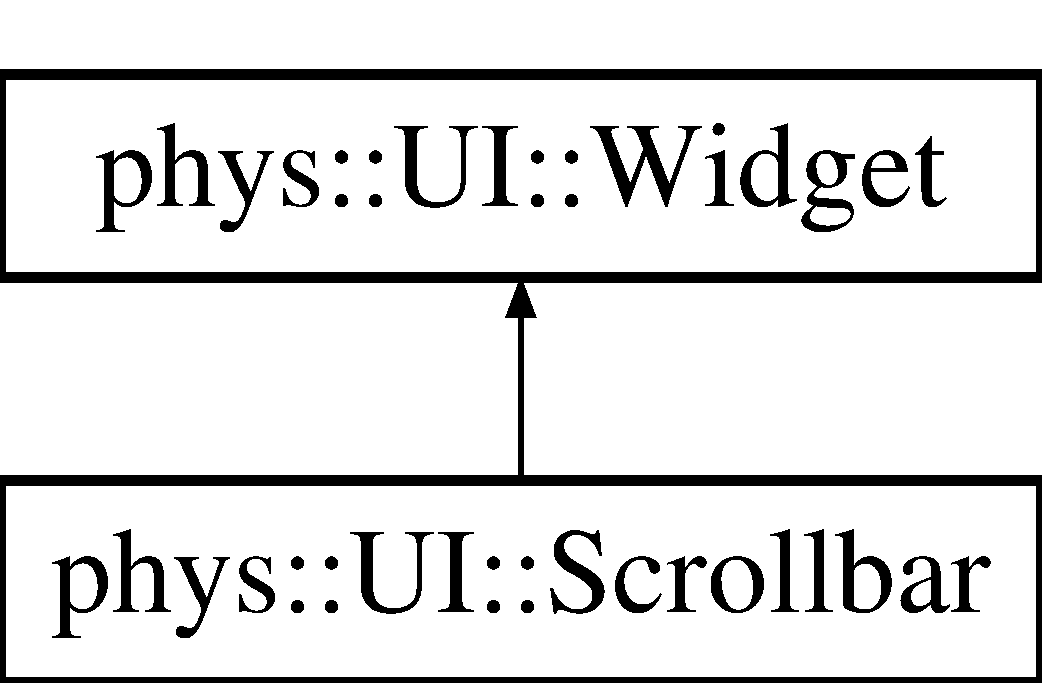
\includegraphics[height=2.000000cm]{d0/d3e/classphys_1_1UI_1_1Scrollbar}
\end{center}
\end{figure}
\subsection*{Public Types}
\begin{DoxyCompactItemize}
\item 
enum {\bfseries BarStyle} \{ {\bfseries NoButtons}, 
{\bfseries Separate}, 
{\bfseries TogetherUpLeft}, 
{\bfseries TogetherDownRight}
 \}
\end{DoxyCompactItemize}
\subsection*{Public Member Functions}
\begin{DoxyCompactItemize}
\item 
\hyperlink{classphys_1_1UI_1_1Scrollbar_a7b095ad5be09dab381c3bd57dd4cb1e4}{Scrollbar} (\hyperlink{namespacephys_aa03900411993de7fbfec4789bc1d392e}{String} \&Name, \hyperlink{classphys_1_1Vector2}{Vector2} Position, \hyperlink{classphys_1_1Vector2}{Vector2} Size, Scrollbar::BarStyle Style, \hyperlink{classphys_1_1UILayer}{UILayer} $\ast$parent)
\begin{DoxyCompactList}\small\item\em Standard initialization constructor. \item\end{DoxyCompactList}\item 
\hypertarget{classphys_1_1UI_1_1Scrollbar_af9fb189c7856353a930c0a228fc0cf42}{
virtual \hyperlink{classphys_1_1UI_1_1Scrollbar_af9fb189c7856353a930c0a228fc0cf42}{$\sim$Scrollbar} ()}
\label{d0/d3e/classphys_1_1UI_1_1Scrollbar_af9fb189c7856353a930c0a228fc0cf42}

\begin{DoxyCompactList}\small\item\em Standard class destructor. \item\end{DoxyCompactList}\item 
virtual bool \hyperlink{classphys_1_1UI_1_1Scrollbar_a8afdd63e36a7fdc15bd8660d9800f2c5}{CheckMouseHover} ()
\begin{DoxyCompactList}\small\item\em Checks to see if the current mouse position is over this widget. \item\end{DoxyCompactList}\item 
virtual \hyperlink{namespacephys_af7eb897198d265b8e868f45240230d5f}{Real} \hyperlink{classphys_1_1UI_1_1Scrollbar_abd70ba640ef9475a77334aa209121812}{GetScrollerValue} ()
\begin{DoxyCompactList}\small\item\em Get the currnent scroll position represented by a value between 0 and 1. \item\end{DoxyCompactList}\item 
virtual void \hyperlink{classphys_1_1UI_1_1Scrollbar_aad3de181a665a2296ae4f6dc1186470d}{SetIncrementDistance} (\hyperlink{namespacephys_af7eb897198d265b8e868f45240230d5f}{Real} IncDist)
\begin{DoxyCompactList}\small\item\em Sets the relative distance the scrollbar will move when the up/left or down/right buttons are pressed. \item\end{DoxyCompactList}\item 
virtual void \hyperlink{classphys_1_1UI_1_1Scrollbar_af5f791a4633e1d090dded18918789a00}{SetScrollerSize} (\hyperlink{namespacephys_af7eb897198d265b8e868f45240230d5f}{Real} Size)
\begin{DoxyCompactList}\small\item\em Sets the length(or height) of the scroller based on the relative size of it's background. \item\end{DoxyCompactList}\item 
virtual void \hyperlink{classphys_1_1UI_1_1Scrollbar_a36d82993b031b7be6da66fff8ca2c2d0}{SetPosition} (\hyperlink{classphys_1_1Vector2}{Vector2} Position)
\begin{DoxyCompactList}\small\item\em Sets the relative position of this widget in pixels. \item\end{DoxyCompactList}\item 
virtual \hyperlink{classphys_1_1Vector2}{Vector2} \hyperlink{classphys_1_1UI_1_1Scrollbar_ad049af26ff2247cfcd988cb5639fa003}{GetPosition} ()
\begin{DoxyCompactList}\small\item\em Gets the relative position of this widget. \item\end{DoxyCompactList}\item 
virtual void \hyperlink{classphys_1_1UI_1_1Scrollbar_ad454fa7b60cfc1359961d553389d7b6f}{SetActualPosition} (\hyperlink{classphys_1_1Vector2}{Vector2} Position)
\begin{DoxyCompactList}\small\item\em Sets the pixel position of this widget. \item\end{DoxyCompactList}\item 
virtual \hyperlink{classphys_1_1Vector2}{Vector2} \hyperlink{classphys_1_1UI_1_1Scrollbar_a73337985c0f1f173e253c88705ae5d6e}{GetActualPosition} ()
\begin{DoxyCompactList}\small\item\em Sets the pixel position of this widget. \item\end{DoxyCompactList}\item 
virtual void \hyperlink{classphys_1_1UI_1_1Scrollbar_ae61511d6f1c7afaf27f2551897d3047d}{SetSize} (\hyperlink{classphys_1_1Vector2}{Vector2} Size)
\begin{DoxyCompactList}\small\item\em Sets the relative size of this widget. \item\end{DoxyCompactList}\item 
virtual \hyperlink{classphys_1_1Vector2}{Vector2} \hyperlink{classphys_1_1UI_1_1Scrollbar_aff97ce371ee21fcf3b648dcf8b38e055}{GetSize} ()
\begin{DoxyCompactList}\small\item\em Gets the relative size of this widget. \item\end{DoxyCompactList}\item 
virtual void \hyperlink{classphys_1_1UI_1_1Scrollbar_a0c543abcd12e168d6084471bd0e0420e}{SetActualSize} (\hyperlink{classphys_1_1Vector2}{Vector2} Size)
\begin{DoxyCompactList}\small\item\em Sets the pixel size of this widget. \item\end{DoxyCompactList}\item 
virtual \hyperlink{classphys_1_1Vector2}{Vector2} \hyperlink{classphys_1_1UI_1_1Scrollbar_a2b3d791cbbe4c787f284d8b12a0edf27}{GetActualSize} ()
\begin{DoxyCompactList}\small\item\em Sets the pixel size of this widget. \item\end{DoxyCompactList}\item 
virtual \hyperlink{classphys_1_1UI_1_1Button}{Button} $\ast$ \hyperlink{classphys_1_1UI_1_1Scrollbar_a0f0d8f4f985198a6bdb8007065fb8663}{GetHoveredButton} ()
\begin{DoxyCompactList}\small\item\em Gets the hovered button within this widget, if any. \item\end{DoxyCompactList}\item 
virtual \hyperlink{classphys_1_1UI_1_1Button}{Button} $\ast$ \hyperlink{classphys_1_1UI_1_1Scrollbar_a28024d2f3a017e4ed3c2a4df62a1e8be}{GetScroller} ()
\begin{DoxyCompactList}\small\item\em Gets the Scroller button within this widget. \item\end{DoxyCompactList}\item 
virtual \hyperlink{classphys_1_1UI_1_1Button}{Button} $\ast$ \hyperlink{classphys_1_1UI_1_1Scrollbar_ab298f9747da2eed451ddce8b1a416c15}{GetUpLeftButton} ()
\begin{DoxyCompactList}\small\item\em Gets the UpLeft button within this widget, if it was initialized. \item\end{DoxyCompactList}\item 
virtual \hyperlink{classphys_1_1UI_1_1Button}{Button} $\ast$ \hyperlink{classphys_1_1UI_1_1Scrollbar_abf733d00087050d575fca1abc2d4ba0e}{GetDownRightButton} ()
\begin{DoxyCompactList}\small\item\em Gets the DownRight button within this widget, if it was initialized. \item\end{DoxyCompactList}\item 
virtual \hyperlink{classphys_1_1UI_1_1Rectangle}{Rectangle} $\ast$ \hyperlink{classphys_1_1UI_1_1Scrollbar_a1c24fbb88f9d86aff1b2f0abc033116a}{GetScrollBack} ()
\begin{DoxyCompactList}\small\item\em Gets the Scroller background within this widget. \item\end{DoxyCompactList}\end{DoxyCompactItemize}
\subsection*{Protected Member Functions}
\begin{DoxyCompactItemize}
\item 
void \hyperlink{classphys_1_1UI_1_1Scrollbar_a9cdd95f31c579b5f7f8631c9dbe1778b}{CreateHorizontalScrollbar} (\hyperlink{classphys_1_1Vector2}{Vector2} Position, \hyperlink{classphys_1_1Vector2}{Vector2} Size)
\begin{DoxyCompactList}\small\item\em Constructor helper function for creating a horizontally aligned scrollbar. \item\end{DoxyCompactList}\item 
void \hyperlink{classphys_1_1UI_1_1Scrollbar_af691e35d62a74925584482f901696ad4}{CreateVerticalScrollbar} (\hyperlink{classphys_1_1Vector2}{Vector2} Position, \hyperlink{classphys_1_1Vector2}{Vector2} Size)
\begin{DoxyCompactList}\small\item\em Constructor helper function for creating a vertically aligned scrollbar. \item\end{DoxyCompactList}\item 
bool \hyperlink{classphys_1_1UI_1_1Scrollbar_ad2989b3f14f11f7c6ec167377487d8a3}{IsValidDimensions} (\hyperlink{classphys_1_1Vector2}{Vector2} \&Size)
\begin{DoxyCompactList}\small\item\em Determines if the dimensions passed into this object are valid and can be used. \item\end{DoxyCompactList}\item 
void \hyperlink{classphys_1_1UI_1_1Scrollbar_abc3671abd06d152f2db526cb0fd4766d}{SetHorizontal} (\hyperlink{classphys_1_1Vector2}{Vector2} \&Size)
\begin{DoxyCompactList}\small\item\em Sets the horizontal perameter as necessary based on the size provided for the widget. \item\end{DoxyCompactList}\item 
void \hyperlink{classphys_1_1UI_1_1Scrollbar_a8a114e8163e5bb29b97c8c32b55095fc}{CalculateOffsets} (\hyperlink{classphys_1_1Vector2}{Vector2} \&Size)
\begin{DoxyCompactList}\small\item\em Calculates the relative offsets for the UI elements that make up this widget. \item\end{DoxyCompactList}\item 
void \hyperlink{classphys_1_1UI_1_1Scrollbar_aa59e2c0662ac13fac037164c86f829f5}{CalculateScrollLimits} ()
\begin{DoxyCompactList}\small\item\em Calculates the limits by which the scroller is allowed to move. \item\end{DoxyCompactList}\item 
void \hyperlink{classphys_1_1UI_1_1Scrollbar_afc9eb290c8dcf3935e2b3046063989e9}{CalculateScrollValue} ()
\begin{DoxyCompactList}\small\item\em Calculates the scrollbar value based on the scrollers current position. \item\end{DoxyCompactList}\item 
void \hyperlink{classphys_1_1UI_1_1Scrollbar_a2048345c29ba15b8820971492f2bdea1}{SetToWithinLimits} (\hyperlink{namespacephys_af7eb897198d265b8e868f45240230d5f}{Real} \&Coord)
\begin{DoxyCompactList}\small\item\em Checks if a provided coordinate is within the defined limits, and adjusts it if not. \item\end{DoxyCompactList}\item 
void \hyperlink{classphys_1_1UI_1_1Scrollbar_a3293265621c49afcd9529f0ca8fb7209}{SetLocation} (\hyperlink{classphys_1_1Vector2}{Vector2} \&Position)
\begin{DoxyCompactList}\small\item\em Internal function for setting the location(position) of this widget. \item\end{DoxyCompactList}\item 
void \hyperlink{classphys_1_1UI_1_1Scrollbar_a7a5bbde7202248b3c094543c1fce3705}{SetArea} (\hyperlink{classphys_1_1Vector2}{Vector2} \&Size)
\begin{DoxyCompactList}\small\item\em Internal function for setting the area(size) of this widget. \item\end{DoxyCompactList}\item 
void \hyperlink{classphys_1_1UI_1_1Scrollbar_a31a2e11f27f087154fd61d7cc2cd6dc1}{ButtonScroll} (bool UpLeft)
\begin{DoxyCompactList}\small\item\em Scrolls the scroller either up/left or down/right, based on the parameter. For use with buttons. \item\end{DoxyCompactList}\item 
void \hyperlink{classphys_1_1UI_1_1Scrollbar_a27e252073b9987b274b574f8159de87e}{MouseScroll} (\hyperlink{classphys_1_1Vector2}{Vector2} Scroll)
\begin{DoxyCompactList}\small\item\em Scrolls the scroller either up/left or down/right. For use with the mouse. \item\end{DoxyCompactList}\item 
void \hyperlink{classphys_1_1UI_1_1Scrollbar_a1c6ca6b135d09d284b31fda2230c9286}{ScrollBackScroll} ()
\begin{DoxyCompactList}\small\item\em Scrolls the scroller either up/left or down/right. For use with the scrollback. \item\end{DoxyCompactList}\item 
virtual void \hyperlink{classphys_1_1UI_1_1Scrollbar_a628999b4caa32f3c273d45e64d5c62a0}{Update} (bool Force=false)
\begin{DoxyCompactList}\small\item\em Performs all the necessary update and automation processes for this widget. \item\end{DoxyCompactList}\end{DoxyCompactItemize}
\subsection*{Protected Attributes}
\begin{DoxyCompactItemize}
\item 
\hypertarget{classphys_1_1UI_1_1Scrollbar_a8ba94ec51f1f43360b0ba5db53e66b80}{
\hyperlink{classphys_1_1UI_1_1Button}{UI::Button} $\ast$ {\bfseries Scroller}}
\label{d0/d3e/classphys_1_1UI_1_1Scrollbar_a8ba94ec51f1f43360b0ba5db53e66b80}

\item 
\hypertarget{classphys_1_1UI_1_1Scrollbar_a4d75376bd2552c1cc699f53d053d94a3}{
\hyperlink{classphys_1_1UI_1_1Rectangle}{UI::Rectangle} $\ast$ {\bfseries ScrollBack}}
\label{d0/d3e/classphys_1_1UI_1_1Scrollbar_a4d75376bd2552c1cc699f53d053d94a3}

\item 
\hypertarget{classphys_1_1UI_1_1Scrollbar_ad26cf0a164ce7fb68b1d2ac12c643bb6}{
\hyperlink{classphys_1_1UI_1_1Button}{UI::Button} $\ast$ {\bfseries UpLeftButton}}
\label{d0/d3e/classphys_1_1UI_1_1Scrollbar_ad26cf0a164ce7fb68b1d2ac12c643bb6}

\item 
\hypertarget{classphys_1_1UI_1_1Scrollbar_a3c5a881c5b752320687729e363e3c829}{
\hyperlink{classphys_1_1UI_1_1Button}{UI::Button} $\ast$ {\bfseries DownRightButton}}
\label{d0/d3e/classphys_1_1UI_1_1Scrollbar_a3c5a881c5b752320687729e363e3c829}

\item 
\hypertarget{classphys_1_1UI_1_1Scrollbar_a0b07b8f9553df84788df6b12ef68eb2b}{
\hyperlink{classphys_1_1UI_1_1Button}{UI::Button} $\ast$ {\bfseries HoveredButton}}
\label{d0/d3e/classphys_1_1UI_1_1Scrollbar_a0b07b8f9553df84788df6b12ef68eb2b}

\item 
\hypertarget{classphys_1_1UI_1_1Scrollbar_ac87b0be84fa48e36cdfa25473d0c720f}{
\hyperlink{classphys_1_1UI_1_1Rectangle}{UI::Rectangle} $\ast$ {\bfseries HoveredBack}}
\label{d0/d3e/classphys_1_1UI_1_1Scrollbar_ac87b0be84fa48e36cdfa25473d0c720f}

\item 
\hypertarget{classphys_1_1UI_1_1Scrollbar_af3be8970f658c345a49a86ef437ad03e}{
\hyperlink{classphys_1_1Vector2}{Vector2} {\bfseries ScrollBackOffset}}
\label{d0/d3e/classphys_1_1UI_1_1Scrollbar_af3be8970f658c345a49a86ef437ad03e}

\item 
\hypertarget{classphys_1_1UI_1_1Scrollbar_abfc66ada8456f085f5d8dfcb9f9f19f1}{
\hyperlink{classphys_1_1Vector2}{Vector2} {\bfseries UpLeftButtonOffset}}
\label{d0/d3e/classphys_1_1UI_1_1Scrollbar_abfc66ada8456f085f5d8dfcb9f9f19f1}

\item 
\hypertarget{classphys_1_1UI_1_1Scrollbar_adee823001982ec29bd5d8ea4b3ed3959}{
\hyperlink{classphys_1_1Vector2}{Vector2} {\bfseries DownRightButtonOffset}}
\label{d0/d3e/classphys_1_1UI_1_1Scrollbar_adee823001982ec29bd5d8ea4b3ed3959}

\item 
\hypertarget{classphys_1_1UI_1_1Scrollbar_a7aeffef5b28306e912e23571b5f690e1}{
\hyperlink{namespacephys_af7eb897198d265b8e868f45240230d5f}{Real} {\bfseries ScrollerUpperLimit}}
\label{d0/d3e/classphys_1_1UI_1_1Scrollbar_a7aeffef5b28306e912e23571b5f690e1}

\item 
\hypertarget{classphys_1_1UI_1_1Scrollbar_a29e5e2fd8b70f8b2663d0594b49f2174}{
\hyperlink{namespacephys_af7eb897198d265b8e868f45240230d5f}{Real} {\bfseries ScrollerLowerLimit}}
\label{d0/d3e/classphys_1_1UI_1_1Scrollbar_a29e5e2fd8b70f8b2663d0594b49f2174}

\item 
\hypertarget{classphys_1_1UI_1_1Scrollbar_ab6ad474b7ad0282cce7aad9cca3a3ed8}{
\hyperlink{namespacephys_af7eb897198d265b8e868f45240230d5f}{Real} {\bfseries ScrollerValue}}
\label{d0/d3e/classphys_1_1UI_1_1Scrollbar_ab6ad474b7ad0282cce7aad9cca3a3ed8}

\item 
\hypertarget{classphys_1_1UI_1_1Scrollbar_a1bb288a799ad346588942806b85b4477}{
\hyperlink{namespacephys_af7eb897198d265b8e868f45240230d5f}{Real} {\bfseries IncrementDistance}}
\label{d0/d3e/classphys_1_1UI_1_1Scrollbar_a1bb288a799ad346588942806b85b4477}

\item 
\hypertarget{classphys_1_1UI_1_1Scrollbar_ac14526cdad2e2046638767dc166e9cdc}{
BarStyle {\bfseries ScrollStyle}}
\label{d0/d3e/classphys_1_1UI_1_1Scrollbar_ac14526cdad2e2046638767dc166e9cdc}

\item 
\hypertarget{classphys_1_1UI_1_1Scrollbar_ac370fd2917bf654e5650087fff21c8ae}{
bool {\bfseries Horizontal}}
\label{d0/d3e/classphys_1_1UI_1_1Scrollbar_ac370fd2917bf654e5650087fff21c8ae}

\item 
\hypertarget{classphys_1_1UI_1_1Scrollbar_ac1eb9202a09c2ab00c033f304787fb50}{
bool {\bfseries ScrollerLock}}
\label{d0/d3e/classphys_1_1UI_1_1Scrollbar_ac1eb9202a09c2ab00c033f304787fb50}

\item 
\hypertarget{classphys_1_1UI_1_1Scrollbar_a10a45c7c3aad71f760b419412786eb8c}{
bool {\bfseries UpLeftLock}}
\label{d0/d3e/classphys_1_1UI_1_1Scrollbar_a10a45c7c3aad71f760b419412786eb8c}

\item 
\hypertarget{classphys_1_1UI_1_1Scrollbar_a133c6d99a33147a62826f0e0c925fcec}{
bool {\bfseries DownRightLock}}
\label{d0/d3e/classphys_1_1UI_1_1Scrollbar_a133c6d99a33147a62826f0e0c925fcec}

\end{DoxyCompactItemize}
\subsection*{Friends}
\begin{DoxyCompactItemize}
\item 
\hypertarget{classphys_1_1UI_1_1Scrollbar_a4b52bf8c4d934bf192ccfc8198b55394}{
class \hyperlink{classphys_1_1UI_1_1Scrollbar_a4b52bf8c4d934bf192ccfc8198b55394}{phys::UIManager}}
\label{d0/d3e/classphys_1_1UI_1_1Scrollbar_a4b52bf8c4d934bf192ccfc8198b55394}

\end{DoxyCompactItemize}


\subsection{Detailed Description}
This class is a widget class, to be used alongside any scrollable widget. If you want to have buttons to accompany your scrollbar they'll automatically have their height match the width of the scrollbar if it's vertical, or their width match their height of the scrollbar if it's horizontal, based on the dimensions provided. \par
 Scrollbars can come in a few styles. Separate is the typical way to present them with the Up or Left button being located at the top of left side of the scroller respectively. Together is where both scroll buttons are next to each other instead of on opposite sides of the scroller. 

Definition at line 67 of file uiscrollbar.h.



\subsection{Constructor \& Destructor Documentation}
\hypertarget{classphys_1_1UI_1_1Scrollbar_a7b095ad5be09dab381c3bd57dd4cb1e4}{
\index{phys::UI::Scrollbar@{phys::UI::Scrollbar}!Scrollbar@{Scrollbar}}
\index{Scrollbar@{Scrollbar}!phys::UI::Scrollbar@{phys::UI::Scrollbar}}
\subsubsection[{Scrollbar}]{\setlength{\rightskip}{0pt plus 5cm}phys::UI::Scrollbar::Scrollbar (
\begin{DoxyParamCaption}
\item[{{\bf String} \&}]{ Name, }
\item[{{\bf Vector2}}]{ Position, }
\item[{{\bf Vector2}}]{ Size, }
\item[{Scrollbar::BarStyle}]{ Style, }
\item[{{\bf UILayer} $\ast$}]{ parent}
\end{DoxyParamCaption}
)}}
\label{d0/d3e/classphys_1_1UI_1_1Scrollbar_a7b095ad5be09dab381c3bd57dd4cb1e4}


Standard initialization constructor. 


\begin{DoxyParams}{Parameters}
\item[{\em Name}]The name of this scrollbar. \item[{\em Position}]A vector2 representing the top left position for this widget to be placed on screen. \item[{\em Size}]A vector2 representing the size of this widget. \item[{\em Style}]An enum value representing how you want your scrollbar constructed. See class details for more info. \item[{\em parent}]The Layer that created this scrollbar. \end{DoxyParams}


Definition at line 54 of file uiscrollbar.cpp.



\subsection{Member Function Documentation}
\hypertarget{classphys_1_1UI_1_1Scrollbar_a31a2e11f27f087154fd61d7cc2cd6dc1}{
\index{phys::UI::Scrollbar@{phys::UI::Scrollbar}!ButtonScroll@{ButtonScroll}}
\index{ButtonScroll@{ButtonScroll}!phys::UI::Scrollbar@{phys::UI::Scrollbar}}
\subsubsection[{ButtonScroll}]{\setlength{\rightskip}{0pt plus 5cm}void phys::UI::Scrollbar::ButtonScroll (
\begin{DoxyParamCaption}
\item[{bool}]{ UpLeft}
\end{DoxyParamCaption}
)\hspace{0.3cm}{\ttfamily  \mbox{[}protected\mbox{]}}}}
\label{d0/d3e/classphys_1_1UI_1_1Scrollbar_a31a2e11f27f087154fd61d7cc2cd6dc1}


Scrolls the scroller either up/left or down/right, based on the parameter. For use with buttons. 

\begin{DoxyInternal}{For internal use only.}
\end{DoxyInternal}


Definition at line 377 of file uiscrollbar.cpp.

\hypertarget{classphys_1_1UI_1_1Scrollbar_a8a114e8163e5bb29b97c8c32b55095fc}{
\index{phys::UI::Scrollbar@{phys::UI::Scrollbar}!CalculateOffsets@{CalculateOffsets}}
\index{CalculateOffsets@{CalculateOffsets}!phys::UI::Scrollbar@{phys::UI::Scrollbar}}
\subsubsection[{CalculateOffsets}]{\setlength{\rightskip}{0pt plus 5cm}void phys::UI::Scrollbar::CalculateOffsets (
\begin{DoxyParamCaption}
\item[{{\bf Vector2} \&}]{ Size}
\end{DoxyParamCaption}
)\hspace{0.3cm}{\ttfamily  \mbox{[}protected\mbox{]}}}}
\label{d0/d3e/classphys_1_1UI_1_1Scrollbar_a8a114e8163e5bb29b97c8c32b55095fc}


Calculates the relative offsets for the UI elements that make up this widget. 

\begin{DoxyInternal}{For internal use only.}
\end{DoxyInternal}


Definition at line 239 of file uiscrollbar.cpp.

\hypertarget{classphys_1_1UI_1_1Scrollbar_aa59e2c0662ac13fac037164c86f829f5}{
\index{phys::UI::Scrollbar@{phys::UI::Scrollbar}!CalculateScrollLimits@{CalculateScrollLimits}}
\index{CalculateScrollLimits@{CalculateScrollLimits}!phys::UI::Scrollbar@{phys::UI::Scrollbar}}
\subsubsection[{CalculateScrollLimits}]{\setlength{\rightskip}{0pt plus 5cm}void phys::UI::Scrollbar::CalculateScrollLimits (
\begin{DoxyParamCaption}
{}
\end{DoxyParamCaption}
)\hspace{0.3cm}{\ttfamily  \mbox{[}protected\mbox{]}}}}
\label{d0/d3e/classphys_1_1UI_1_1Scrollbar_aa59e2c0662ac13fac037164c86f829f5}


Calculates the limits by which the scroller is allowed to move. 

\begin{DoxyInternal}{For internal use only.}
\end{DoxyInternal}


Definition at line 283 of file uiscrollbar.cpp.

\hypertarget{classphys_1_1UI_1_1Scrollbar_afc9eb290c8dcf3935e2b3046063989e9}{
\index{phys::UI::Scrollbar@{phys::UI::Scrollbar}!CalculateScrollValue@{CalculateScrollValue}}
\index{CalculateScrollValue@{CalculateScrollValue}!phys::UI::Scrollbar@{phys::UI::Scrollbar}}
\subsubsection[{CalculateScrollValue}]{\setlength{\rightskip}{0pt plus 5cm}void phys::UI::Scrollbar::CalculateScrollValue (
\begin{DoxyParamCaption}
{}
\end{DoxyParamCaption}
)\hspace{0.3cm}{\ttfamily  \mbox{[}protected\mbox{]}}}}
\label{d0/d3e/classphys_1_1UI_1_1Scrollbar_afc9eb290c8dcf3935e2b3046063989e9}


Calculates the scrollbar value based on the scrollers current position. 

\begin{DoxyInternal}{For internal use only.}
\end{DoxyInternal}


Definition at line 295 of file uiscrollbar.cpp.

\hypertarget{classphys_1_1UI_1_1Scrollbar_a8afdd63e36a7fdc15bd8660d9800f2c5}{
\index{phys::UI::Scrollbar@{phys::UI::Scrollbar}!CheckMouseHover@{CheckMouseHover}}
\index{CheckMouseHover@{CheckMouseHover}!phys::UI::Scrollbar@{phys::UI::Scrollbar}}
\subsubsection[{CheckMouseHover}]{\setlength{\rightskip}{0pt plus 5cm}bool phys::UI::Scrollbar::CheckMouseHover (
\begin{DoxyParamCaption}
{}
\end{DoxyParamCaption}
)\hspace{0.3cm}{\ttfamily  \mbox{[}virtual\mbox{]}}}}
\label{d0/d3e/classphys_1_1UI_1_1Scrollbar_a8afdd63e36a7fdc15bd8660d9800f2c5}


Checks to see if the current mouse position is over this widget. 

\begin{DoxyReturn}{Returns}
Returns a bool value, true if the mouse is over this widget, false if it's not. 
\end{DoxyReturn}


Implements \hyperlink{classphys_1_1UI_1_1Widget_a613df6dbb42efe139d185043a00259dc}{phys::UI::Widget}.



Definition at line 515 of file uiscrollbar.cpp.

\hypertarget{classphys_1_1UI_1_1Scrollbar_a9cdd95f31c579b5f7f8631c9dbe1778b}{
\index{phys::UI::Scrollbar@{phys::UI::Scrollbar}!CreateHorizontalScrollbar@{CreateHorizontalScrollbar}}
\index{CreateHorizontalScrollbar@{CreateHorizontalScrollbar}!phys::UI::Scrollbar@{phys::UI::Scrollbar}}
\subsubsection[{CreateHorizontalScrollbar}]{\setlength{\rightskip}{0pt plus 5cm}void phys::UI::Scrollbar::CreateHorizontalScrollbar (
\begin{DoxyParamCaption}
\item[{{\bf Vector2}}]{ Position, }
\item[{{\bf Vector2}}]{ Size}
\end{DoxyParamCaption}
)\hspace{0.3cm}{\ttfamily  \mbox{[}protected\mbox{]}}}}
\label{d0/d3e/classphys_1_1UI_1_1Scrollbar_a9cdd95f31c579b5f7f8631c9dbe1778b}


Constructor helper function for creating a horizontally aligned scrollbar. 

\begin{DoxyInternal}{For internal use only.}
\end{DoxyInternal}


Definition at line 94 of file uiscrollbar.cpp.

\hypertarget{classphys_1_1UI_1_1Scrollbar_af691e35d62a74925584482f901696ad4}{
\index{phys::UI::Scrollbar@{phys::UI::Scrollbar}!CreateVerticalScrollbar@{CreateVerticalScrollbar}}
\index{CreateVerticalScrollbar@{CreateVerticalScrollbar}!phys::UI::Scrollbar@{phys::UI::Scrollbar}}
\subsubsection[{CreateVerticalScrollbar}]{\setlength{\rightskip}{0pt plus 5cm}void phys::UI::Scrollbar::CreateVerticalScrollbar (
\begin{DoxyParamCaption}
\item[{{\bf Vector2}}]{ Position, }
\item[{{\bf Vector2}}]{ Size}
\end{DoxyParamCaption}
)\hspace{0.3cm}{\ttfamily  \mbox{[}protected\mbox{]}}}}
\label{d0/d3e/classphys_1_1UI_1_1Scrollbar_af691e35d62a74925584482f901696ad4}


Constructor helper function for creating a vertically aligned scrollbar. 

\begin{DoxyInternal}{For internal use only.}
\end{DoxyInternal}


Definition at line 154 of file uiscrollbar.cpp.

\hypertarget{classphys_1_1UI_1_1Scrollbar_a73337985c0f1f173e253c88705ae5d6e}{
\index{phys::UI::Scrollbar@{phys::UI::Scrollbar}!GetActualPosition@{GetActualPosition}}
\index{GetActualPosition@{GetActualPosition}!phys::UI::Scrollbar@{phys::UI::Scrollbar}}
\subsubsection[{GetActualPosition}]{\setlength{\rightskip}{0pt plus 5cm}{\bf Vector2} phys::UI::Scrollbar::GetActualPosition (
\begin{DoxyParamCaption}
{}
\end{DoxyParamCaption}
)\hspace{0.3cm}{\ttfamily  \mbox{[}virtual\mbox{]}}}}
\label{d0/d3e/classphys_1_1UI_1_1Scrollbar_a73337985c0f1f173e253c88705ae5d6e}


Sets the pixel position of this widget. 

\begin{DoxyReturn}{Returns}
Returns a vector2 representing the pixel position of this widget. 
\end{DoxyReturn}


Implements \hyperlink{classphys_1_1UI_1_1Widget_a0a29fecff7f56d7909f65fd63b0990e7}{phys::UI::Widget}.



Definition at line 596 of file uiscrollbar.cpp.

\hypertarget{classphys_1_1UI_1_1Scrollbar_a2b3d791cbbe4c787f284d8b12a0edf27}{
\index{phys::UI::Scrollbar@{phys::UI::Scrollbar}!GetActualSize@{GetActualSize}}
\index{GetActualSize@{GetActualSize}!phys::UI::Scrollbar@{phys::UI::Scrollbar}}
\subsubsection[{GetActualSize}]{\setlength{\rightskip}{0pt plus 5cm}{\bf Vector2} phys::UI::Scrollbar::GetActualSize (
\begin{DoxyParamCaption}
{}
\end{DoxyParamCaption}
)\hspace{0.3cm}{\ttfamily  \mbox{[}virtual\mbox{]}}}}
\label{d0/d3e/classphys_1_1UI_1_1Scrollbar_a2b3d791cbbe4c787f284d8b12a0edf27}


Sets the pixel size of this widget. 

\begin{DoxyReturn}{Returns}
Returns a vector2 representing the pixel size of this widget. 
\end{DoxyReturn}


Implements \hyperlink{classphys_1_1UI_1_1Widget_af3a685621ed220748c0940ea38c96ed2}{phys::UI::Widget}.



Definition at line 641 of file uiscrollbar.cpp.

\hypertarget{classphys_1_1UI_1_1Scrollbar_abf733d00087050d575fca1abc2d4ba0e}{
\index{phys::UI::Scrollbar@{phys::UI::Scrollbar}!GetDownRightButton@{GetDownRightButton}}
\index{GetDownRightButton@{GetDownRightButton}!phys::UI::Scrollbar@{phys::UI::Scrollbar}}
\subsubsection[{GetDownRightButton}]{\setlength{\rightskip}{0pt plus 5cm}{\bf Button} $\ast$ phys::UI::Scrollbar::GetDownRightButton (
\begin{DoxyParamCaption}
{}
\end{DoxyParamCaption}
)\hspace{0.3cm}{\ttfamily  \mbox{[}virtual\mbox{]}}}}
\label{d0/d3e/classphys_1_1UI_1_1Scrollbar_abf733d00087050d575fca1abc2d4ba0e}


Gets the DownRight button within this widget, if it was initialized. 

\begin{DoxyReturn}{Returns}
Returns a pointer to the DownRight button within this widget, or NULL if none. 
\end{DoxyReturn}


Definition at line 676 of file uiscrollbar.cpp.

\hypertarget{classphys_1_1UI_1_1Scrollbar_a0f0d8f4f985198a6bdb8007065fb8663}{
\index{phys::UI::Scrollbar@{phys::UI::Scrollbar}!GetHoveredButton@{GetHoveredButton}}
\index{GetHoveredButton@{GetHoveredButton}!phys::UI::Scrollbar@{phys::UI::Scrollbar}}
\subsubsection[{GetHoveredButton}]{\setlength{\rightskip}{0pt plus 5cm}{\bf Button} $\ast$ phys::UI::Scrollbar::GetHoveredButton (
\begin{DoxyParamCaption}
{}
\end{DoxyParamCaption}
)\hspace{0.3cm}{\ttfamily  \mbox{[}virtual\mbox{]}}}}
\label{d0/d3e/classphys_1_1UI_1_1Scrollbar_a0f0d8f4f985198a6bdb8007065fb8663}


Gets the hovered button within this widget, if any. 

\begin{DoxyReturn}{Returns}
Returns a pointer to the button within this widget the mouse is hovering over, or NULL if none. 
\end{DoxyReturn}


Definition at line 661 of file uiscrollbar.cpp.

\hypertarget{classphys_1_1UI_1_1Scrollbar_ad049af26ff2247cfcd988cb5639fa003}{
\index{phys::UI::Scrollbar@{phys::UI::Scrollbar}!GetPosition@{GetPosition}}
\index{GetPosition@{GetPosition}!phys::UI::Scrollbar@{phys::UI::Scrollbar}}
\subsubsection[{GetPosition}]{\setlength{\rightskip}{0pt plus 5cm}{\bf Vector2} phys::UI::Scrollbar::GetPosition (
\begin{DoxyParamCaption}
{}
\end{DoxyParamCaption}
)\hspace{0.3cm}{\ttfamily  \mbox{[}virtual\mbox{]}}}}
\label{d0/d3e/classphys_1_1UI_1_1Scrollbar_ad049af26ff2247cfcd988cb5639fa003}


Gets the relative position of this widget. 

The position is relative to the screen size. Values range from 0.0 to 1.0. \begin{DoxyReturn}{Returns}
Returns a vector2 representing the relative position of this widget. 
\end{DoxyReturn}


Implements \hyperlink{classphys_1_1UI_1_1Widget_a3e464b028b0d1b5755923b8790260c33}{phys::UI::Widget}.



Definition at line 585 of file uiscrollbar.cpp.

\hypertarget{classphys_1_1UI_1_1Scrollbar_a1c24fbb88f9d86aff1b2f0abc033116a}{
\index{phys::UI::Scrollbar@{phys::UI::Scrollbar}!GetScrollBack@{GetScrollBack}}
\index{GetScrollBack@{GetScrollBack}!phys::UI::Scrollbar@{phys::UI::Scrollbar}}
\subsubsection[{GetScrollBack}]{\setlength{\rightskip}{0pt plus 5cm}{\bf Rectangle} $\ast$ phys::UI::Scrollbar::GetScrollBack (
\begin{DoxyParamCaption}
{}
\end{DoxyParamCaption}
)\hspace{0.3cm}{\ttfamily  \mbox{[}virtual\mbox{]}}}}
\label{d0/d3e/classphys_1_1UI_1_1Scrollbar_a1c24fbb88f9d86aff1b2f0abc033116a}


Gets the Scroller background within this widget. 

\begin{DoxyReturn}{Returns}
Returns a pointer to the Scroller background within this widget. 
\end{DoxyReturn}


Definition at line 681 of file uiscrollbar.cpp.

\hypertarget{classphys_1_1UI_1_1Scrollbar_a28024d2f3a017e4ed3c2a4df62a1e8be}{
\index{phys::UI::Scrollbar@{phys::UI::Scrollbar}!GetScroller@{GetScroller}}
\index{GetScroller@{GetScroller}!phys::UI::Scrollbar@{phys::UI::Scrollbar}}
\subsubsection[{GetScroller}]{\setlength{\rightskip}{0pt plus 5cm}{\bf Button} $\ast$ phys::UI::Scrollbar::GetScroller (
\begin{DoxyParamCaption}
{}
\end{DoxyParamCaption}
)\hspace{0.3cm}{\ttfamily  \mbox{[}virtual\mbox{]}}}}
\label{d0/d3e/classphys_1_1UI_1_1Scrollbar_a28024d2f3a017e4ed3c2a4df62a1e8be}


Gets the Scroller button within this widget. 

\begin{DoxyReturn}{Returns}
Returns a pointer to the Scroller button within this widget. 
\end{DoxyReturn}


Definition at line 666 of file uiscrollbar.cpp.

\hypertarget{classphys_1_1UI_1_1Scrollbar_abd70ba640ef9475a77334aa209121812}{
\index{phys::UI::Scrollbar@{phys::UI::Scrollbar}!GetScrollerValue@{GetScrollerValue}}
\index{GetScrollerValue@{GetScrollerValue}!phys::UI::Scrollbar@{phys::UI::Scrollbar}}
\subsubsection[{GetScrollerValue}]{\setlength{\rightskip}{0pt plus 5cm}{\bf Real} phys::UI::Scrollbar::GetScrollerValue (
\begin{DoxyParamCaption}
{}
\end{DoxyParamCaption}
)\hspace{0.3cm}{\ttfamily  \mbox{[}virtual\mbox{]}}}}
\label{d0/d3e/classphys_1_1UI_1_1Scrollbar_abd70ba640ef9475a77334aa209121812}


Get the currnent scroll position represented by a value between 0 and 1. 

For example, if the scroller is halfway down the limits it's allowed, this will return 0.5. \par
 Like other values, the top and left represent origin(0) values. \begin{DoxyReturn}{Returns}
Returns the stored scroll position. 
\end{DoxyReturn}


Definition at line 552 of file uiscrollbar.cpp.

\hypertarget{classphys_1_1UI_1_1Scrollbar_aff97ce371ee21fcf3b648dcf8b38e055}{
\index{phys::UI::Scrollbar@{phys::UI::Scrollbar}!GetSize@{GetSize}}
\index{GetSize@{GetSize}!phys::UI::Scrollbar@{phys::UI::Scrollbar}}
\subsubsection[{GetSize}]{\setlength{\rightskip}{0pt plus 5cm}{\bf Vector2} phys::UI::Scrollbar::GetSize (
\begin{DoxyParamCaption}
{}
\end{DoxyParamCaption}
)\hspace{0.3cm}{\ttfamily  \mbox{[}virtual\mbox{]}}}}
\label{d0/d3e/classphys_1_1UI_1_1Scrollbar_aff97ce371ee21fcf3b648dcf8b38e055}


Gets the relative size of this widget. 

The size is relative to the screen size. Values range from 0.0 to 1.0. \begin{DoxyReturn}{Returns}
Returns a vector2 representing the relative size of this widget. 
\end{DoxyReturn}


Implements \hyperlink{classphys_1_1UI_1_1Widget_a07039c19e57de314147ce066417da0a2}{phys::UI::Widget}.



Definition at line 619 of file uiscrollbar.cpp.

\hypertarget{classphys_1_1UI_1_1Scrollbar_ab298f9747da2eed451ddce8b1a416c15}{
\index{phys::UI::Scrollbar@{phys::UI::Scrollbar}!GetUpLeftButton@{GetUpLeftButton}}
\index{GetUpLeftButton@{GetUpLeftButton}!phys::UI::Scrollbar@{phys::UI::Scrollbar}}
\subsubsection[{GetUpLeftButton}]{\setlength{\rightskip}{0pt plus 5cm}{\bf Button} $\ast$ phys::UI::Scrollbar::GetUpLeftButton (
\begin{DoxyParamCaption}
{}
\end{DoxyParamCaption}
)\hspace{0.3cm}{\ttfamily  \mbox{[}virtual\mbox{]}}}}
\label{d0/d3e/classphys_1_1UI_1_1Scrollbar_ab298f9747da2eed451ddce8b1a416c15}


Gets the UpLeft button within this widget, if it was initialized. 

\begin{DoxyReturn}{Returns}
Returns a pointer to the UpLeft button within this widget, or NULL if none. 
\end{DoxyReturn}


Definition at line 671 of file uiscrollbar.cpp.

\hypertarget{classphys_1_1UI_1_1Scrollbar_ad2989b3f14f11f7c6ec167377487d8a3}{
\index{phys::UI::Scrollbar@{phys::UI::Scrollbar}!IsValidDimensions@{IsValidDimensions}}
\index{IsValidDimensions@{IsValidDimensions}!phys::UI::Scrollbar@{phys::UI::Scrollbar}}
\subsubsection[{IsValidDimensions}]{\setlength{\rightskip}{0pt plus 5cm}bool phys::UI::Scrollbar::IsValidDimensions (
\begin{DoxyParamCaption}
\item[{{\bf Vector2} \&}]{ Size}
\end{DoxyParamCaption}
)\hspace{0.3cm}{\ttfamily  \mbox{[}protected\mbox{]}}}}
\label{d0/d3e/classphys_1_1UI_1_1Scrollbar_ad2989b3f14f11f7c6ec167377487d8a3}


Determines if the dimensions passed into this object are valid and can be used. 

\begin{DoxyInternal}{For internal use only.}
\end{DoxyInternal}


Definition at line 214 of file uiscrollbar.cpp.

\hypertarget{classphys_1_1UI_1_1Scrollbar_a27e252073b9987b274b574f8159de87e}{
\index{phys::UI::Scrollbar@{phys::UI::Scrollbar}!MouseScroll@{MouseScroll}}
\index{MouseScroll@{MouseScroll}!phys::UI::Scrollbar@{phys::UI::Scrollbar}}
\subsubsection[{MouseScroll}]{\setlength{\rightskip}{0pt plus 5cm}void phys::UI::Scrollbar::MouseScroll (
\begin{DoxyParamCaption}
\item[{{\bf Vector2}}]{ Scroll}
\end{DoxyParamCaption}
)\hspace{0.3cm}{\ttfamily  \mbox{[}protected\mbox{]}}}}
\label{d0/d3e/classphys_1_1UI_1_1Scrollbar_a27e252073b9987b274b574f8159de87e}


Scrolls the scroller either up/left or down/right. For use with the mouse. 

\begin{DoxyInternal}{For internal use only.}
\end{DoxyInternal}


Definition at line 399 of file uiscrollbar.cpp.

\hypertarget{classphys_1_1UI_1_1Scrollbar_a1c6ca6b135d09d284b31fda2230c9286}{
\index{phys::UI::Scrollbar@{phys::UI::Scrollbar}!ScrollBackScroll@{ScrollBackScroll}}
\index{ScrollBackScroll@{ScrollBackScroll}!phys::UI::Scrollbar@{phys::UI::Scrollbar}}
\subsubsection[{ScrollBackScroll}]{\setlength{\rightskip}{0pt plus 5cm}void phys::UI::Scrollbar::ScrollBackScroll (
\begin{DoxyParamCaption}
{}
\end{DoxyParamCaption}
)\hspace{0.3cm}{\ttfamily  \mbox{[}protected\mbox{]}}}}
\label{d0/d3e/classphys_1_1UI_1_1Scrollbar_a1c6ca6b135d09d284b31fda2230c9286}


Scrolls the scroller either up/left or down/right. For use with the scrollback. 

\begin{DoxyInternal}{For internal use only.}
\end{DoxyInternal}


Definition at line 418 of file uiscrollbar.cpp.

\hypertarget{classphys_1_1UI_1_1Scrollbar_ad454fa7b60cfc1359961d553389d7b6f}{
\index{phys::UI::Scrollbar@{phys::UI::Scrollbar}!SetActualPosition@{SetActualPosition}}
\index{SetActualPosition@{SetActualPosition}!phys::UI::Scrollbar@{phys::UI::Scrollbar}}
\subsubsection[{SetActualPosition}]{\setlength{\rightskip}{0pt plus 5cm}void phys::UI::Scrollbar::SetActualPosition (
\begin{DoxyParamCaption}
\item[{{\bf Vector2}}]{ Position}
\end{DoxyParamCaption}
)\hspace{0.3cm}{\ttfamily  \mbox{[}virtual\mbox{]}}}}
\label{d0/d3e/classphys_1_1UI_1_1Scrollbar_ad454fa7b60cfc1359961d553389d7b6f}


Sets the pixel position of this widget. 


\begin{DoxyParams}{Parameters}
\item[{\em Position}]A vector2 representing the pixel position of this widget. \end{DoxyParams}


Implements \hyperlink{classphys_1_1UI_1_1Widget_ac8f70c390e7724e57fc99e51d8004a9b}{phys::UI::Widget}.



Definition at line 590 of file uiscrollbar.cpp.

\hypertarget{classphys_1_1UI_1_1Scrollbar_a0c543abcd12e168d6084471bd0e0420e}{
\index{phys::UI::Scrollbar@{phys::UI::Scrollbar}!SetActualSize@{SetActualSize}}
\index{SetActualSize@{SetActualSize}!phys::UI::Scrollbar@{phys::UI::Scrollbar}}
\subsubsection[{SetActualSize}]{\setlength{\rightskip}{0pt plus 5cm}void phys::UI::Scrollbar::SetActualSize (
\begin{DoxyParamCaption}
\item[{{\bf Vector2}}]{ Size}
\end{DoxyParamCaption}
)\hspace{0.3cm}{\ttfamily  \mbox{[}virtual\mbox{]}}}}
\label{d0/d3e/classphys_1_1UI_1_1Scrollbar_a0c543abcd12e168d6084471bd0e0420e}


Sets the pixel size of this widget. 


\begin{DoxyParams}{Parameters}
\item[{\em Size}]A vector2 representing the pixel size of this widget. \end{DoxyParams}


Implements \hyperlink{classphys_1_1UI_1_1Widget_a8ceb54fd067847844b314dedd8e529f8}{phys::UI::Widget}.



Definition at line 624 of file uiscrollbar.cpp.

\hypertarget{classphys_1_1UI_1_1Scrollbar_a7a5bbde7202248b3c094543c1fce3705}{
\index{phys::UI::Scrollbar@{phys::UI::Scrollbar}!SetArea@{SetArea}}
\index{SetArea@{SetArea}!phys::UI::Scrollbar@{phys::UI::Scrollbar}}
\subsubsection[{SetArea}]{\setlength{\rightskip}{0pt plus 5cm}void phys::UI::Scrollbar::SetArea (
\begin{DoxyParamCaption}
\item[{{\bf Vector2} \&}]{ Size}
\end{DoxyParamCaption}
)\hspace{0.3cm}{\ttfamily  \mbox{[}protected\mbox{]}}}}
\label{d0/d3e/classphys_1_1UI_1_1Scrollbar_a7a5bbde7202248b3c094543c1fce3705}


Internal function for setting the area(size) of this widget. 

\begin{DoxyInternal}{For internal use only.}
\end{DoxyInternal}


Definition at line 350 of file uiscrollbar.cpp.

\hypertarget{classphys_1_1UI_1_1Scrollbar_abc3671abd06d152f2db526cb0fd4766d}{
\index{phys::UI::Scrollbar@{phys::UI::Scrollbar}!SetHorizontal@{SetHorizontal}}
\index{SetHorizontal@{SetHorizontal}!phys::UI::Scrollbar@{phys::UI::Scrollbar}}
\subsubsection[{SetHorizontal}]{\setlength{\rightskip}{0pt plus 5cm}void phys::UI::Scrollbar::SetHorizontal (
\begin{DoxyParamCaption}
\item[{{\bf Vector2} \&}]{ Size}
\end{DoxyParamCaption}
)\hspace{0.3cm}{\ttfamily  \mbox{[}protected\mbox{]}}}}
\label{d0/d3e/classphys_1_1UI_1_1Scrollbar_abc3671abd06d152f2db526cb0fd4766d}


Sets the horizontal perameter as necessary based on the size provided for the widget. 

\begin{DoxyInternal}{For internal use only.}
\end{DoxyInternal}


Definition at line 227 of file uiscrollbar.cpp.

\hypertarget{classphys_1_1UI_1_1Scrollbar_aad3de181a665a2296ae4f6dc1186470d}{
\index{phys::UI::Scrollbar@{phys::UI::Scrollbar}!SetIncrementDistance@{SetIncrementDistance}}
\index{SetIncrementDistance@{SetIncrementDistance}!phys::UI::Scrollbar@{phys::UI::Scrollbar}}
\subsubsection[{SetIncrementDistance}]{\setlength{\rightskip}{0pt plus 5cm}void phys::UI::Scrollbar::SetIncrementDistance (
\begin{DoxyParamCaption}
\item[{{\bf Real}}]{ IncDist}
\end{DoxyParamCaption}
)\hspace{0.3cm}{\ttfamily  \mbox{[}virtual\mbox{]}}}}
\label{d0/d3e/classphys_1_1UI_1_1Scrollbar_aad3de181a665a2296ae4f6dc1186470d}


Sets the relative distance the scrollbar will move when the up/left or down/right buttons are pressed. 


\begin{DoxyParams}{Parameters}
\item[{\em IncDist}]A real representing the amount to increment. Can be negative. \end{DoxyParams}


Definition at line 557 of file uiscrollbar.cpp.

\hypertarget{classphys_1_1UI_1_1Scrollbar_a3293265621c49afcd9529f0ca8fb7209}{
\index{phys::UI::Scrollbar@{phys::UI::Scrollbar}!SetLocation@{SetLocation}}
\index{SetLocation@{SetLocation}!phys::UI::Scrollbar@{phys::UI::Scrollbar}}
\subsubsection[{SetLocation}]{\setlength{\rightskip}{0pt plus 5cm}void phys::UI::Scrollbar::SetLocation (
\begin{DoxyParamCaption}
\item[{{\bf Vector2} \&}]{ Position}
\end{DoxyParamCaption}
)\hspace{0.3cm}{\ttfamily  \mbox{[}protected\mbox{]}}}}
\label{d0/d3e/classphys_1_1UI_1_1Scrollbar_a3293265621c49afcd9529f0ca8fb7209}


Internal function for setting the location(position) of this widget. 

\begin{DoxyInternal}{For internal use only.}
\end{DoxyInternal}


Definition at line 328 of file uiscrollbar.cpp.

\hypertarget{classphys_1_1UI_1_1Scrollbar_a36d82993b031b7be6da66fff8ca2c2d0}{
\index{phys::UI::Scrollbar@{phys::UI::Scrollbar}!SetPosition@{SetPosition}}
\index{SetPosition@{SetPosition}!phys::UI::Scrollbar@{phys::UI::Scrollbar}}
\subsubsection[{SetPosition}]{\setlength{\rightskip}{0pt plus 5cm}void phys::UI::Scrollbar::SetPosition (
\begin{DoxyParamCaption}
\item[{{\bf Vector2}}]{ Position}
\end{DoxyParamCaption}
)\hspace{0.3cm}{\ttfamily  \mbox{[}virtual\mbox{]}}}}
\label{d0/d3e/classphys_1_1UI_1_1Scrollbar_a36d82993b031b7be6da66fff8ca2c2d0}


Sets the relative position of this widget in pixels. 

The position is relative to the screen size. Values range from 0.0 to 1.0. \par
 The top and the left are considered the origin, thus values of 0 represent one of these points. 
\begin{DoxyParams}{Parameters}
\item[{\em Position}]A vector2 representing the relative position of this widget. \end{DoxyParams}


Implements \hyperlink{classphys_1_1UI_1_1Widget_aae1c0b891125823e7ade8cbc7e4ba6b6}{phys::UI::Widget}.



Definition at line 578 of file uiscrollbar.cpp.

\hypertarget{classphys_1_1UI_1_1Scrollbar_af5f791a4633e1d090dded18918789a00}{
\index{phys::UI::Scrollbar@{phys::UI::Scrollbar}!SetScrollerSize@{SetScrollerSize}}
\index{SetScrollerSize@{SetScrollerSize}!phys::UI::Scrollbar@{phys::UI::Scrollbar}}
\subsubsection[{SetScrollerSize}]{\setlength{\rightskip}{0pt plus 5cm}void phys::UI::Scrollbar::SetScrollerSize (
\begin{DoxyParamCaption}
\item[{{\bf Real}}]{ Size}
\end{DoxyParamCaption}
)\hspace{0.3cm}{\ttfamily  \mbox{[}virtual\mbox{]}}}}
\label{d0/d3e/classphys_1_1UI_1_1Scrollbar_af5f791a4633e1d090dded18918789a00}


Sets the length(or height) of the scroller based on the relative size of it's background. 


\begin{DoxyParams}{Parameters}
\item[{\em Size}]The relative size you with to set the scroller to. Values range from 0.0 to 1.0. \end{DoxyParams}


Definition at line 562 of file uiscrollbar.cpp.

\hypertarget{classphys_1_1UI_1_1Scrollbar_ae61511d6f1c7afaf27f2551897d3047d}{
\index{phys::UI::Scrollbar@{phys::UI::Scrollbar}!SetSize@{SetSize}}
\index{SetSize@{SetSize}!phys::UI::Scrollbar@{phys::UI::Scrollbar}}
\subsubsection[{SetSize}]{\setlength{\rightskip}{0pt plus 5cm}void phys::UI::Scrollbar::SetSize (
\begin{DoxyParamCaption}
\item[{{\bf Vector2}}]{ Size}
\end{DoxyParamCaption}
)\hspace{0.3cm}{\ttfamily  \mbox{[}virtual\mbox{]}}}}
\label{d0/d3e/classphys_1_1UI_1_1Scrollbar_ae61511d6f1c7afaf27f2551897d3047d}


Sets the relative size of this widget. 


\begin{DoxyParams}{Parameters}
\item[{\em Size}]A vector2 representing the relative size of this widget. \end{DoxyParams}


Implements \hyperlink{classphys_1_1UI_1_1Widget_ad5af5f04b60d43341037df6b0e329bbd}{phys::UI::Widget}.



Definition at line 601 of file uiscrollbar.cpp.

\hypertarget{classphys_1_1UI_1_1Scrollbar_a2048345c29ba15b8820971492f2bdea1}{
\index{phys::UI::Scrollbar@{phys::UI::Scrollbar}!SetToWithinLimits@{SetToWithinLimits}}
\index{SetToWithinLimits@{SetToWithinLimits}!phys::UI::Scrollbar@{phys::UI::Scrollbar}}
\subsubsection[{SetToWithinLimits}]{\setlength{\rightskip}{0pt plus 5cm}void phys::UI::Scrollbar::SetToWithinLimits (
\begin{DoxyParamCaption}
\item[{{\bf Real} \&}]{ Coord}
\end{DoxyParamCaption}
)\hspace{0.3cm}{\ttfamily  \mbox{[}protected\mbox{]}}}}
\label{d0/d3e/classphys_1_1UI_1_1Scrollbar_a2048345c29ba15b8820971492f2bdea1}


Checks if a provided coordinate is within the defined limits, and adjusts it if not. 

\begin{DoxyInternal}{For internal use only.}
\end{DoxyInternal}


Definition at line 309 of file uiscrollbar.cpp.

\hypertarget{classphys_1_1UI_1_1Scrollbar_a628999b4caa32f3c273d45e64d5c62a0}{
\index{phys::UI::Scrollbar@{phys::UI::Scrollbar}!Update@{Update}}
\index{Update@{Update}!phys::UI::Scrollbar@{phys::UI::Scrollbar}}
\subsubsection[{Update}]{\setlength{\rightskip}{0pt plus 5cm}void phys::UI::Scrollbar::Update (
\begin{DoxyParamCaption}
\item[{bool}]{ Force = {\ttfamily false}}
\end{DoxyParamCaption}
)\hspace{0.3cm}{\ttfamily  \mbox{[}protected, virtual\mbox{]}}}}
\label{d0/d3e/classphys_1_1UI_1_1Scrollbar_a628999b4caa32f3c273d45e64d5c62a0}


Performs all the necessary update and automation processes for this widget. 

\begin{DoxyInternal}{For internal use only.}
\end{DoxyInternal}


Implements \hyperlink{classphys_1_1UI_1_1Widget_a1806425fcd684c2f0d50cd0ef4a6b0da}{phys::UI::Widget}.



Definition at line 449 of file uiscrollbar.cpp.



The documentation for this class was generated from the following files:\begin{DoxyCompactItemize}
\item 
uiscrollbar.h\item 
uiscrollbar.cpp\end{DoxyCompactItemize}

\hypertarget{classphys_1_1SliderConstraint}{
\section{phys::SliderConstraint Class Reference}
\label{dc/d72/classphys_1_1SliderConstraint}\index{phys::SliderConstraint@{phys::SliderConstraint}}
}
Inheritance diagram for phys::SliderConstraint:\begin{figure}[H]
\begin{center}
\leavevmode
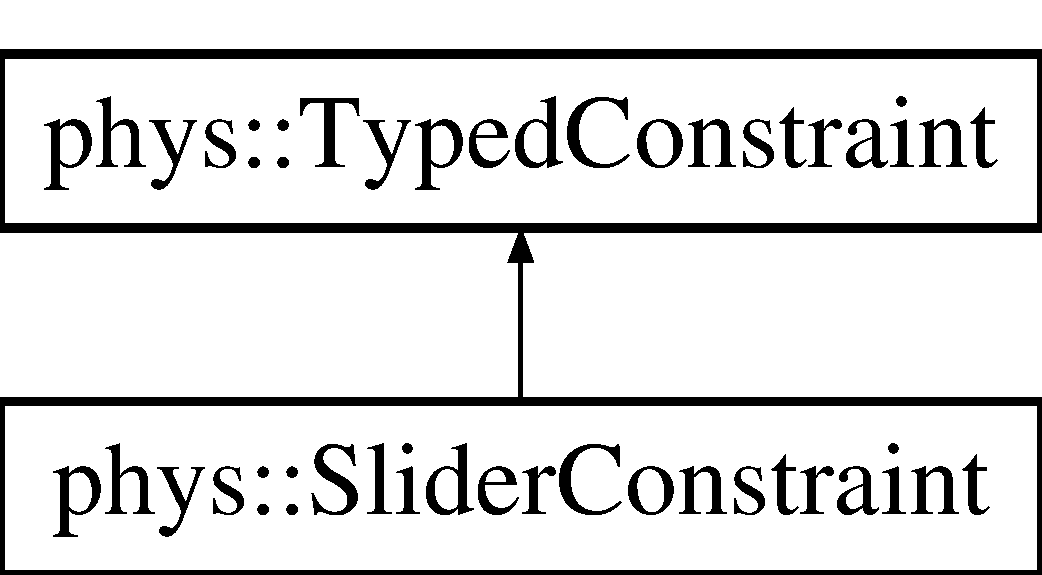
\includegraphics[height=2cm]{dc/d72/classphys_1_1SliderConstraint}
\end{center}
\end{figure}
\subsection*{Public Member Functions}
\begin{DoxyCompactItemize}
\item 
\hypertarget{classphys_1_1SliderConstraint_a012329e9d8125ff030c6351045f0f97b}{
{\bfseries SliderConstraint} (\hyperlink{classphys_1_1ActorRigid}{ActorRigid} $\ast$ActorA, \hyperlink{classphys_1_1ActorRigid}{ActorRigid} $\ast$ActorB, \hyperlink{classphys_1_1Vector3}{Vector3} VectorA, \hyperlink{classphys_1_1Vector3}{Vector3} VectorB, \hyperlink{classphys_1_1Quaternion}{Quaternion} QuaternionA, \hyperlink{classphys_1_1Quaternion}{Quaternion} QuaternionB, bool UseLinearReferenceA)}
\label{dc/d72/classphys_1_1SliderConstraint_a012329e9d8125ff030c6351045f0f97b}

\item 
\hypertarget{classphys_1_1SliderConstraint_a4727dc39e3ac0ab553aa6a1cff00fc4e}{
{\bfseries SliderConstraint} (\hyperlink{classphys_1_1ActorRigid}{ActorRigid} $\ast$ActorB, \hyperlink{classphys_1_1Vector3}{Vector3} VectorB, \hyperlink{classphys_1_1Quaternion}{Quaternion} QuaternionB, bool UseLinearReferenceA)}
\label{dc/d72/classphys_1_1SliderConstraint_a4727dc39e3ac0ab553aa6a1cff00fc4e}

\item 
\hypertarget{classphys_1_1SliderConstraint_a142708184f0a445edadddc4ad5ca08b5}{
{\bfseries SliderConstraint} (btSliderConstraint $\ast$Constraint)}
\label{dc/d72/classphys_1_1SliderConstraint_a142708184f0a445edadddc4ad5ca08b5}

\item 
\hypertarget{classphys_1_1SliderConstraint_a815265abaf184340aef505eaf82775e2}{
void {\bfseries SetFrameOffsetALocation} (\hyperlink{classphys_1_1Vector3}{Vector3} Location)}
\label{dc/d72/classphys_1_1SliderConstraint_a815265abaf184340aef505eaf82775e2}

\item 
\hypertarget{classphys_1_1SliderConstraint_a828eb0ffac6d95ce2d8d9690a12ca722}{
void {\bfseries SetFrameOffsetBLocation} (\hyperlink{classphys_1_1Vector3}{Vector3} Location)}
\label{dc/d72/classphys_1_1SliderConstraint_a828eb0ffac6d95ce2d8d9690a12ca722}

\item 
\hypertarget{classphys_1_1SliderConstraint_a52489284afda499982707f712db6ed99}{
void {\bfseries SetUpperLinLimit} (\hyperlink{namespacephys_af7eb897198d265b8e868f45240230d5f}{Real} UpperLimit)}
\label{dc/d72/classphys_1_1SliderConstraint_a52489284afda499982707f712db6ed99}

\item 
\hypertarget{classphys_1_1SliderConstraint_af441963a725b255ed34f5c82de7088a9}{
void {\bfseries SetUpperAngLimit} (\hyperlink{namespacephys_af7eb897198d265b8e868f45240230d5f}{Real} UpperLimit)}
\label{dc/d72/classphys_1_1SliderConstraint_af441963a725b255ed34f5c82de7088a9}

\item 
\hypertarget{classphys_1_1SliderConstraint_acf651cb8a31ca8730935a745a5555251}{
void {\bfseries SetLowerLinLimit} (\hyperlink{namespacephys_af7eb897198d265b8e868f45240230d5f}{Real} LowerLimit)}
\label{dc/d72/classphys_1_1SliderConstraint_acf651cb8a31ca8730935a745a5555251}

\item 
\hypertarget{classphys_1_1SliderConstraint_a4cbad2248429018961196e8aa91b89e8}{
void {\bfseries SetLowerAngLimit} (\hyperlink{namespacephys_af7eb897198d265b8e868f45240230d5f}{Real} LowerLimit)}
\label{dc/d72/classphys_1_1SliderConstraint_a4cbad2248429018961196e8aa91b89e8}

\item 
\hypertarget{classphys_1_1SliderConstraint_aca541af1afb9859f8991209533152e3c}{
void {\bfseries SetPoweredLinMotor} (bool OnOff)}
\label{dc/d72/classphys_1_1SliderConstraint_aca541af1afb9859f8991209533152e3c}

\item 
\hypertarget{classphys_1_1SliderConstraint_a74ab484d5989397a47de16b76b507e92}{
void {\bfseries SetTargetLinMotorVelocity} (\hyperlink{namespacephys_af7eb897198d265b8e868f45240230d5f}{Real} TargetLinMotorVelocity)}
\label{dc/d72/classphys_1_1SliderConstraint_a74ab484d5989397a47de16b76b507e92}

\item 
\hypertarget{classphys_1_1SliderConstraint_a958485ca8f1abd4e429583db42a909aa}{
void {\bfseries SetMaxLinMotorForce} (\hyperlink{namespacephys_af7eb897198d265b8e868f45240230d5f}{Real} MaxLinMotorForce)}
\label{dc/d72/classphys_1_1SliderConstraint_a958485ca8f1abd4e429583db42a909aa}

\item 
\hypertarget{classphys_1_1SliderConstraint_aafa81adee5bc78b4d435429e9ddcf538}{
void {\bfseries SetPoweredAngMotor} (bool OnOff)}
\label{dc/d72/classphys_1_1SliderConstraint_aafa81adee5bc78b4d435429e9ddcf538}

\item 
\hypertarget{classphys_1_1SliderConstraint_acad0aa3e9b3086956e45c5825570ec10}{
void {\bfseries SetTargetAngMotorVelocity} (\hyperlink{namespacephys_af7eb897198d265b8e868f45240230d5f}{Real} TargetAngMotorVelocity)}
\label{dc/d72/classphys_1_1SliderConstraint_acad0aa3e9b3086956e45c5825570ec10}

\item 
\hypertarget{classphys_1_1SliderConstraint_a2fec0b1834acb78f0a7c2276ff14a991}{
void {\bfseries SetMaxAngMotorForce} (\hyperlink{namespacephys_af7eb897198d265b8e868f45240230d5f}{Real} MaxAngMotorForce)}
\label{dc/d72/classphys_1_1SliderConstraint_a2fec0b1834acb78f0a7c2276ff14a991}

\item 
\hypertarget{classphys_1_1SliderConstraint_ac6800dd5abfe2fd90948967b08398022}{
void {\bfseries SetUseFrameOffset} (bool FrameOffset)}
\label{dc/d72/classphys_1_1SliderConstraint_ac6800dd5abfe2fd90948967b08398022}

\item 
\hypertarget{classphys_1_1SliderConstraint_a96bccd70fb876ee279c942fdd0d14997}{
void {\bfseries SetSoftnessDirLin} (\hyperlink{namespacephys_af7eb897198d265b8e868f45240230d5f}{Real} SoftnessDirLin)}
\label{dc/d72/classphys_1_1SliderConstraint_a96bccd70fb876ee279c942fdd0d14997}

\item 
\hypertarget{classphys_1_1SliderConstraint_ad8fbde22dea580bcbee816d9e1426c14}{
void {\bfseries SetRestitutionDirLin} (\hyperlink{namespacephys_af7eb897198d265b8e868f45240230d5f}{Real} RestitutionDirLin)}
\label{dc/d72/classphys_1_1SliderConstraint_ad8fbde22dea580bcbee816d9e1426c14}

\item 
\hypertarget{classphys_1_1SliderConstraint_aa34acb7592f0de36205919dc82f996e1}{
void {\bfseries SetDampingDirLin} (\hyperlink{namespacephys_af7eb897198d265b8e868f45240230d5f}{Real} DampingDirLin)}
\label{dc/d72/classphys_1_1SliderConstraint_aa34acb7592f0de36205919dc82f996e1}

\item 
\hypertarget{classphys_1_1SliderConstraint_a27e0e6cbad5cb7366dab889a9fda5d0b}{
void {\bfseries SetSoftnessDirAng} (\hyperlink{namespacephys_af7eb897198d265b8e868f45240230d5f}{Real} SoftnessDirAng)}
\label{dc/d72/classphys_1_1SliderConstraint_a27e0e6cbad5cb7366dab889a9fda5d0b}

\item 
\hypertarget{classphys_1_1SliderConstraint_a9c512f3fa92d1116ed1453a52b42e964}{
void {\bfseries SetRestitutionDirAng} (\hyperlink{namespacephys_af7eb897198d265b8e868f45240230d5f}{Real} RestitutionDirAng)}
\label{dc/d72/classphys_1_1SliderConstraint_a9c512f3fa92d1116ed1453a52b42e964}

\item 
\hypertarget{classphys_1_1SliderConstraint_a8c679a3f387fb7e16ee3a7efe7490f3e}{
void {\bfseries SetDampingDirAng} (\hyperlink{namespacephys_af7eb897198d265b8e868f45240230d5f}{Real} DampingDirAng)}
\label{dc/d72/classphys_1_1SliderConstraint_a8c679a3f387fb7e16ee3a7efe7490f3e}

\item 
\hypertarget{classphys_1_1SliderConstraint_a44c260da76b5bb951fc732877f71ede8}{
void {\bfseries SetSoftnessLimLin} (\hyperlink{namespacephys_af7eb897198d265b8e868f45240230d5f}{Real} SoftnessLimLin)}
\label{dc/d72/classphys_1_1SliderConstraint_a44c260da76b5bb951fc732877f71ede8}

\item 
\hypertarget{classphys_1_1SliderConstraint_a70656ab2e9dc8f4c8cef9c815a1d4dac}{
void {\bfseries SetRestitutionLimLin} (\hyperlink{namespacephys_af7eb897198d265b8e868f45240230d5f}{Real} RestitutionLimLin)}
\label{dc/d72/classphys_1_1SliderConstraint_a70656ab2e9dc8f4c8cef9c815a1d4dac}

\item 
\hypertarget{classphys_1_1SliderConstraint_ac8c919a66c932962f8361bd2c9b6004e}{
void {\bfseries SetDampingLimLin} (\hyperlink{namespacephys_af7eb897198d265b8e868f45240230d5f}{Real} DampingLimLin)}
\label{dc/d72/classphys_1_1SliderConstraint_ac8c919a66c932962f8361bd2c9b6004e}

\item 
\hypertarget{classphys_1_1SliderConstraint_a161703d76d6942dee0a9fcd754b8173e}{
void {\bfseries SetSoftnessLimAng} (\hyperlink{namespacephys_af7eb897198d265b8e868f45240230d5f}{Real} SoftnessLimAng)}
\label{dc/d72/classphys_1_1SliderConstraint_a161703d76d6942dee0a9fcd754b8173e}

\item 
\hypertarget{classphys_1_1SliderConstraint_a6c8bb1e2c60ab1f1bcb6bb622f02cc3b}{
void {\bfseries SetRestitutionLimAng} (\hyperlink{namespacephys_af7eb897198d265b8e868f45240230d5f}{Real} RestitutionLimAng)}
\label{dc/d72/classphys_1_1SliderConstraint_a6c8bb1e2c60ab1f1bcb6bb622f02cc3b}

\item 
\hypertarget{classphys_1_1SliderConstraint_ad8a8c8db50f87b550311f15854b341da}{
void {\bfseries SetDampingLimAng} (\hyperlink{namespacephys_af7eb897198d265b8e868f45240230d5f}{Real} DampingLimAng)}
\label{dc/d72/classphys_1_1SliderConstraint_ad8a8c8db50f87b550311f15854b341da}

\item 
\hypertarget{classphys_1_1SliderConstraint_a9b8d07a013fdc6982d8334f60c347cf6}{
void {\bfseries SetSoftnessOrthoLin} (\hyperlink{namespacephys_af7eb897198d265b8e868f45240230d5f}{Real} SoftnessOrthoLin)}
\label{dc/d72/classphys_1_1SliderConstraint_a9b8d07a013fdc6982d8334f60c347cf6}

\item 
\hypertarget{classphys_1_1SliderConstraint_a3f02673645c8dd790a1ea445e566f4b6}{
void {\bfseries SetRestitutionOrthoLin} (\hyperlink{namespacephys_af7eb897198d265b8e868f45240230d5f}{Real} RestitutionOrthoLin)}
\label{dc/d72/classphys_1_1SliderConstraint_a3f02673645c8dd790a1ea445e566f4b6}

\item 
\hypertarget{classphys_1_1SliderConstraint_aa41383cdebe8c6343d5b16fecaebdc35}{
void {\bfseries SetDampingOrthoLin} (\hyperlink{namespacephys_af7eb897198d265b8e868f45240230d5f}{Real} DampingOrthoLin)}
\label{dc/d72/classphys_1_1SliderConstraint_aa41383cdebe8c6343d5b16fecaebdc35}

\item 
\hypertarget{classphys_1_1SliderConstraint_a4efe57a9656ad1686b3aff2b2f9643d0}{
void {\bfseries SetSoftnessOrthoAng} (\hyperlink{namespacephys_af7eb897198d265b8e868f45240230d5f}{Real} SoftnessOrthoAng)}
\label{dc/d72/classphys_1_1SliderConstraint_a4efe57a9656ad1686b3aff2b2f9643d0}

\item 
\hypertarget{classphys_1_1SliderConstraint_ada0a9eab21ef9ac48d711cb67c69a989}{
void {\bfseries SetRestitutionOrthoAng} (\hyperlink{namespacephys_af7eb897198d265b8e868f45240230d5f}{Real} RestitutionOrthoAng)}
\label{dc/d72/classphys_1_1SliderConstraint_ada0a9eab21ef9ac48d711cb67c69a989}

\item 
\hypertarget{classphys_1_1SliderConstraint_a85e6748c60d9b036bf53033233067586}{
void {\bfseries SetDampingOrthoAng} (\hyperlink{namespacephys_af7eb897198d265b8e868f45240230d5f}{Real} DampingOrthoAng)}
\label{dc/d72/classphys_1_1SliderConstraint_a85e6748c60d9b036bf53033233067586}

\item 
\hypertarget{classphys_1_1SliderConstraint_a1516aeff86674a969411b17a1847d115}{
virtual void {\bfseries SetParam} (int num, \hyperlink{namespacephys_af7eb897198d265b8e868f45240230d5f}{Real} value, int axis=-\/1)}
\label{dc/d72/classphys_1_1SliderConstraint_a1516aeff86674a969411b17a1847d115}

\item 
\hypertarget{classphys_1_1SliderConstraint_a181393c2beec42bdebf7d1a17dfe7593}{
virtual \hyperlink{namespacephys_af7eb897198d265b8e868f45240230d5f}{Real} {\bfseries GetParam} (int num, int axis=-\/1)}
\label{dc/d72/classphys_1_1SliderConstraint_a181393c2beec42bdebf7d1a17dfe7593}

\end{DoxyCompactItemize}
\subsection*{Protected Attributes}
\begin{DoxyCompactItemize}
\item 
\hypertarget{classphys_1_1SliderConstraint_ae99629f3e87f72d3271ff82137fa81e2}{
btSliderConstraint $\ast$ {\bfseries Slider}}
\label{dc/d72/classphys_1_1SliderConstraint_ae99629f3e87f72d3271ff82137fa81e2}

\end{DoxyCompactItemize}


\subsection{Detailed Description}


Definition at line 191 of file constraint.h.



The documentation for this class was generated from the following files:\begin{DoxyCompactItemize}
\item 
constraint.h\item 
constraint.cpp\end{DoxyCompactItemize}

\hypertarget{classphys_1_1Sound}{
\section{phys::Sound Class Reference}
\label{dc/d2f/classphys_1_1Sound}\index{phys::Sound@{phys::Sound}}
}


\hyperlink{structThis}{This} is an instance of a sound that can be played and manipulated.  




{\ttfamily \#include $<$sound.h$>$}

\subsection*{Public Member Functions}
\begin{DoxyCompactItemize}
\item 
\hyperlink{classphys_1_1Sound_a6a9d4b475da9453c9b02ca2c49a6fa76}{Sound} ()
\begin{DoxyCompactList}\small\item\em Class Constructor. Internal use only. \item\end{DoxyCompactList}\item 
\hyperlink{classphys_1_1Sound_a0452d6079bcb201f9d2f3b2742eb21b6}{Sound} (cAudio::IAudioSource $\ast$Source, cAudio::IAudioManager $\ast$manager)
\begin{DoxyCompactList}\small\item\em Class Constructor. Internal use only. \item\end{DoxyCompactList}\item 
\hyperlink{classphys_1_1Sound_ad49df56479e003d0990a5dcb1c506d39}{$\sim$Sound} ()
\begin{DoxyCompactList}\small\item\em Class destructor. \item\end{DoxyCompactList}\item 
void \hyperlink{classphys_1_1Sound_ae7caa90deb9e5a4cab2d5ada27f5e5b5}{Play} ()
\begin{DoxyCompactList}\small\item\em Plays the sound. \item\end{DoxyCompactList}\item 
void \hyperlink{classphys_1_1Sound_a853bb9a2c1b41cd82a385608614861e7}{Play2d} (bool Loop=false)
\begin{DoxyCompactList}\small\item\em Plays the sound in 2D mode. \item\end{DoxyCompactList}\item 
void \hyperlink{classphys_1_1Sound_adbb79c9d1a37bf541bfb259551c6067f}{Play3d} (\hyperlink{classphys_1_1Vector3}{Vector3} Position, \hyperlink{namespacephys_af7eb897198d265b8e868f45240230d5f}{Real} SoundStrength=1.0, bool Loop=false)
\begin{DoxyCompactList}\small\item\em Plays the sound in 3D mode. \item\end{DoxyCompactList}\item 
void \hyperlink{classphys_1_1Sound_a805bef416bec70b5e250dd29e622cf46}{Pause} ()
\item 
void \hyperlink{classphys_1_1Sound_a662d760ec0e6214537b13810a8ac9955}{Stop} ()
\item 
void \hyperlink{classphys_1_1Sound_afd5645195ac744de62c5eefc01dbf0d0}{Loop} (bool ToLoop)
\begin{DoxyCompactList}\small\item\em Sets whether this sound should loop. \item\end{DoxyCompactList}\item 
void \hyperlink{classphys_1_1Sound_a8dfc3b7e9419a3c50c0ac6ecf6ece096}{Seek} (\hyperlink{namespacephys_af7eb897198d265b8e868f45240230d5f}{Real} Seconds, bool Relative)
\begin{DoxyCompactList}\small\item\em Allows you to go to a specific point in the sound. \item\end{DoxyCompactList}\item 
\hyperlink{namespacephys_af7eb897198d265b8e868f45240230d5f}{Real} \hyperlink{classphys_1_1Sound_a2c3864cbc6c25cd9a47529c75dea142b}{GetTotalAudioTime} ()
\begin{DoxyCompactList}\small\item\em Gets the total size of the sound in seconds. \item\end{DoxyCompactList}\item 
int \hyperlink{classphys_1_1Sound_a2891732590e4276a64583ee9bdab555e}{GetTotalAudioSize} ()
\begin{DoxyCompactList}\small\item\em Gets the total size of the sound in memory. \item\end{DoxyCompactList}\item 
int \hyperlink{classphys_1_1Sound_af568fd5293ecab6185f509e52209a0a2}{GetCompressedAudioSize} ()
\begin{DoxyCompactList}\small\item\em Gets the original compressed size of the sound. \item\end{DoxyCompactList}\item 
\hyperlink{namespacephys_af7eb897198d265b8e868f45240230d5f}{Real} \hyperlink{classphys_1_1Sound_ace3c118ee42540be51dcf64940d4f1e0}{GetCurrentAudioTime} ()
\begin{DoxyCompactList}\small\item\em Gets the current position in the audio stream in seconds. \item\end{DoxyCompactList}\item 
int \hyperlink{classphys_1_1Sound_a0ef4ddd4096758f9c883fe93194b9b3b}{GetCurrentAudioPosition} ()
\begin{DoxyCompactList}\small\item\em Gets the current position in the audio stream in bytes. \item\end{DoxyCompactList}\item 
int \hyperlink{classphys_1_1Sound_adbcd16d55670bc6d97a1ce9b3d22d90c}{GetCurrentCompressedAudioPosition} ()
\begin{DoxyCompactList}\small\item\em Gets the current position in the original audio stream in bytes. \item\end{DoxyCompactList}\item 
bool \hyperlink{classphys_1_1Sound_a382b26fd5289da4fdb2b536e953b7ea0}{IsPlaying} ()
\begin{DoxyCompactList}\small\item\em Checks to see if the sound is currently playing. \item\end{DoxyCompactList}\item 
bool \hyperlink{classphys_1_1Sound_a21ad445ca3e3b4836ee838c41584d8c1}{IsPaused} ()
\begin{DoxyCompactList}\small\item\em Checks to see if the sound is currently paused. \item\end{DoxyCompactList}\item 
bool \hyperlink{classphys_1_1Sound_ac35ba604ca2aaab246e5ce5f524d10f9}{IsStopped} ()
\begin{DoxyCompactList}\small\item\em Checks to see if the sound is currently stopped. \item\end{DoxyCompactList}\item 
bool \hyperlink{classphys_1_1Sound_a67f4a5475bc634c8ee894933cc09f933}{IsLooping} ()
\begin{DoxyCompactList}\small\item\em Checks to see if the sound is currently set to loop. \item\end{DoxyCompactList}\item 
void \hyperlink{classphys_1_1Sound_a245bc4d760bcf30e9520aee00cf40c61}{SetPosition} (\hyperlink{classphys_1_1Vector3}{Vector3} Position)
\begin{DoxyCompactList}\small\item\em Sets the position of the sound source. \item\end{DoxyCompactList}\item 
void \hyperlink{classphys_1_1Sound_a673a0ab44fa32fdcd15180e813b7b02b}{SetVelocity} (\hyperlink{classphys_1_1Vector3}{Vector3} Velocity)
\begin{DoxyCompactList}\small\item\em Sets the velocity of the sound source. \item\end{DoxyCompactList}\item 
void \hyperlink{classphys_1_1Sound_af2d6aa7e1b3b2e9f60b8dbbe8aa2d381}{SetDirection} (\hyperlink{classphys_1_1Vector3}{Vector3} Direction)
\begin{DoxyCompactList}\small\item\em Sets the direction the sound source is facing. \item\end{DoxyCompactList}\item 
void \hyperlink{classphys_1_1Sound_a56e657013dc4d561dbc3b0c5d12d542d}{SetRolloffFactor} (\hyperlink{namespacephys_af7eb897198d265b8e868f45240230d5f}{Real} Rolloff)
\begin{DoxyCompactList}\small\item\em Sets the Rolloff factor used to attenuate the sound over a distance. \item\end{DoxyCompactList}\item 
void \hyperlink{classphys_1_1Sound_a44d6c066fad6f09553e47892a14bf5ef}{SetStrength} (\hyperlink{namespacephys_af7eb897198d265b8e868f45240230d5f}{Real} SoundStrength)
\begin{DoxyCompactList}\small\item\em Sets the strength of the sound source. \item\end{DoxyCompactList}\item 
void \hyperlink{classphys_1_1Sound_ae32d4c4b8a09bfbdcfea68cfa71aa354}{SetMinDistance} (\hyperlink{namespacephys_af7eb897198d265b8e868f45240230d5f}{Real} MinDistance)
\begin{DoxyCompactList}\small\item\em Sets the distance from the sound source where attenuation will start. \item\end{DoxyCompactList}\item 
void \hyperlink{classphys_1_1Sound_a54d04549f0851b00736fdab18a81ec70}{SetMaxDistance} (\hyperlink{namespacephys_af7eb897198d265b8e868f45240230d5f}{Real} MaxDistance)
\begin{DoxyCompactList}\small\item\em Sets the distance from the sound source where attenuation will stop. \item\end{DoxyCompactList}\item 
void \hyperlink{classphys_1_1Sound_a4c7eac57c162f264d8c0868c4f360aab}{SetPitch} (\hyperlink{namespacephys_af7eb897198d265b8e868f45240230d5f}{Real} Pitch)
\begin{DoxyCompactList}\small\item\em Sets the pitch of the sound source. \item\end{DoxyCompactList}\item 
void \hyperlink{classphys_1_1Sound_a62438fb7916e1e7e9abe66722de83821}{SetVolume} (\hyperlink{namespacephys_af7eb897198d265b8e868f45240230d5f}{Real} Volume)
\begin{DoxyCompactList}\small\item\em Sets the current volume of the sound source before effects. \item\end{DoxyCompactList}\item 
void \hyperlink{classphys_1_1Sound_a76a487c8a455556ba4307c99cc41ea80}{SetMinVolume} (\hyperlink{namespacephys_af7eb897198d265b8e868f45240230d5f}{Real} MinVolume)
\begin{DoxyCompactList}\small\item\em Sets the minimum volume the sound source can achieve. \item\end{DoxyCompactList}\item 
void \hyperlink{classphys_1_1Sound_a04994399e336c8a0726c5da9f6349545}{SetMaxVolume} (\hyperlink{namespacephys_af7eb897198d265b8e868f45240230d5f}{Real} MaxVolume)
\begin{DoxyCompactList}\small\item\em Sets the maximum volume the sound source can achieve. \item\end{DoxyCompactList}\item 
void \hyperlink{classphys_1_1Sound_ae231936d44db727eb48f9ff259ae0dd6}{SetInnerConeAngle} (\hyperlink{namespacephys_af7eb897198d265b8e868f45240230d5f}{Real} InnerAngle)
\begin{DoxyCompactList}\small\item\em Sets the inner cone angle of the sound source if you want the sound to be projected as a cone. \item\end{DoxyCompactList}\item 
void \hyperlink{classphys_1_1Sound_a4fc7d07d303ddb97acc15524950d0442}{SetOuterConeAngle} (\hyperlink{namespacephys_af7eb897198d265b8e868f45240230d5f}{Real} OuterAngle)
\begin{DoxyCompactList}\small\item\em Sets the outer cone angle of the sound source if you want the sound to be projected as a cone. \item\end{DoxyCompactList}\item 
void \hyperlink{classphys_1_1Sound_a55b0eadd492fc1a5fbae9848f5682ac9}{SetOuterConeVolume} (\hyperlink{namespacephys_af7eb897198d265b8e868f45240230d5f}{Real} OuterVolume)
\begin{DoxyCompactList}\small\item\em Sets how much the volume is scaled in the outer cone. \item\end{DoxyCompactList}\item 
void \hyperlink{classphys_1_1Sound_a159a5ac92577b55e86a8fc2dbf8bc806}{SetDopplerStrength} (\hyperlink{namespacephys_af7eb897198d265b8e868f45240230d5f}{Real} DopStr)
\begin{DoxyCompactList}\small\item\em Sets the doppler strength, which impacts the doppler effect. \item\end{DoxyCompactList}\item 
void \hyperlink{classphys_1_1Sound_a5a7f337dbc533f49269f736f51d25b85}{SetDopplerVelocity} (\hyperlink{classphys_1_1Vector3}{Vector3} Velocity)
\begin{DoxyCompactList}\small\item\em Sets the doppler velocity vector. \item\end{DoxyCompactList}\item 
void \hyperlink{classphys_1_1Sound_a62075a732f25c0a07b428c09c6232814}{Move} (\hyperlink{classphys_1_1Vector3}{Vector3} Position)
\begin{DoxyCompactList}\small\item\em Moves the sound source. \item\end{DoxyCompactList}\item 
\hyperlink{classphys_1_1Vector3}{Vector3} \hyperlink{classphys_1_1Sound_a6d7097965cb87491896f688a8ef12d45}{GetPosition} ()
\begin{DoxyCompactList}\small\item\em Gets the objects position. \item\end{DoxyCompactList}\item 
\hyperlink{classphys_1_1Vector3}{Vector3} \hyperlink{classphys_1_1Sound_a48e996b687ec11ff1d19400a010c4f07}{GetVelocity} ()
\begin{DoxyCompactList}\small\item\em Gets the objects velocity. \item\end{DoxyCompactList}\item 
\hyperlink{classphys_1_1Vector3}{Vector3} \hyperlink{classphys_1_1Sound_a228e07cbcf0c8fee7b0f1f86a0162484}{GetDirection} ()
\begin{DoxyCompactList}\small\item\em Gets the objects direction. \item\end{DoxyCompactList}\item 
\hyperlink{namespacephys_af7eb897198d265b8e868f45240230d5f}{Real} \hyperlink{classphys_1_1Sound_ab87182be43ed55e44acf7143a7b08213}{GetRolloffFactor} ()
\begin{DoxyCompactList}\small\item\em Gets the Rolloff factor of the sound source. \item\end{DoxyCompactList}\item 
\hyperlink{namespacephys_af7eb897198d265b8e868f45240230d5f}{Real} \hyperlink{classphys_1_1Sound_ab839e69523500591b40252e32bafbbb3}{GetStrength} ()
\begin{DoxyCompactList}\small\item\em Gets the Strength of the sound source. \item\end{DoxyCompactList}\item 
\hyperlink{namespacephys_af7eb897198d265b8e868f45240230d5f}{Real} \hyperlink{classphys_1_1Sound_a45534a33db7c3aec3861b44327925bc2}{GetMinDistance} ()
\begin{DoxyCompactList}\small\item\em Gets the distance at which sound attenuation will start. \item\end{DoxyCompactList}\item 
\hyperlink{namespacephys_af7eb897198d265b8e868f45240230d5f}{Real} \hyperlink{classphys_1_1Sound_a5a9868c589bf85bf1775481e0c8fe4d3}{GetMaxDistance} ()
\begin{DoxyCompactList}\small\item\em Gets the distance at which sound attenuation will stop. \item\end{DoxyCompactList}\item 
\hyperlink{namespacephys_af7eb897198d265b8e868f45240230d5f}{Real} \hyperlink{classphys_1_1Sound_ae28ce63dc22eb8a80edf9dbfe8ea64cd}{GetPitch} ()
\begin{DoxyCompactList}\small\item\em Gets the pitch of the sound source. \item\end{DoxyCompactList}\item 
\hyperlink{namespacephys_af7eb897198d265b8e868f45240230d5f}{Real} \hyperlink{classphys_1_1Sound_ad386c2247f87d4b57bfae2c722282417}{GetVolume} ()
\begin{DoxyCompactList}\small\item\em Gets the current volume of the sound source. \item\end{DoxyCompactList}\item 
\hyperlink{namespacephys_af7eb897198d265b8e868f45240230d5f}{Real} \hyperlink{classphys_1_1Sound_a366c57366bbbfc13eea18e1908f19eb4}{GetMinVolume} ()
\begin{DoxyCompactList}\small\item\em Gets the minimum volume of the sound source. \item\end{DoxyCompactList}\item 
\hyperlink{namespacephys_af7eb897198d265b8e868f45240230d5f}{Real} \hyperlink{classphys_1_1Sound_aebda862caeda83fed2789f1e8bfca7ea}{GetMaxVolume} ()
\begin{DoxyCompactList}\small\item\em Gets the Maximum volume of the sound source. \item\end{DoxyCompactList}\item 
\hyperlink{namespacephys_af7eb897198d265b8e868f45240230d5f}{Real} \hyperlink{classphys_1_1Sound_a5e39752133cd5d8d160455bbbcb360fd}{GetInnerConeAngle} ()
\begin{DoxyCompactList}\small\item\em Gets the inner cone angle of the sound source. \item\end{DoxyCompactList}\item 
\hyperlink{namespacephys_af7eb897198d265b8e868f45240230d5f}{Real} \hyperlink{classphys_1_1Sound_ad39ca4504655a777283fd2e238b729d1}{GetOuterConeAngle} ()
\begin{DoxyCompactList}\small\item\em Gets the outer cone angle of the sound source. \item\end{DoxyCompactList}\item 
\hyperlink{namespacephys_af7eb897198d265b8e868f45240230d5f}{Real} \hyperlink{classphys_1_1Sound_a2607037d0c40d32f402d0ebb98586a00}{GetOuterConeVolume} ()
\begin{DoxyCompactList}\small\item\em Gets the outer cone volume of the sound source. \item\end{DoxyCompactList}\item 
\hyperlink{namespacephys_af7eb897198d265b8e868f45240230d5f}{Real} \hyperlink{classphys_1_1Sound_a894e1390d76c6a6e79404569afeaf168}{GetDopplerStrength} ()
\begin{DoxyCompactList}\small\item\em Gets the Doppler Strength of the sound. \item\end{DoxyCompactList}\item 
\hyperlink{classphys_1_1Vector3}{Vector3} \hyperlink{classphys_1_1Sound_a9d4e845004b59ba5bdc066f7f12ff7d7}{GetDopplerVelocity} ()
\begin{DoxyCompactList}\small\item\em Gets the doppler velocity vector. \item\end{DoxyCompactList}\end{DoxyCompactItemize}
\subsection*{Protected Attributes}
\begin{DoxyCompactItemize}
\item 
\hypertarget{classphys_1_1Sound_a7cd63202ea3dbc96c6f466a60b89b0fe}{
cAudio::IAudioSource $\ast$ {\bfseries SoundSource}}
\label{dc/d2f/classphys_1_1Sound_a7cd63202ea3dbc96c6f466a60b89b0fe}

\item 
\hypertarget{classphys_1_1Sound_a84b31e91bd1363ba430a51f579a07e0b}{
cAudio::IAudioManager $\ast$ {\bfseries Manager}}
\label{dc/d2f/classphys_1_1Sound_a84b31e91bd1363ba430a51f579a07e0b}

\end{DoxyCompactItemize}
\subsection*{Friends}
\begin{DoxyCompactItemize}
\item 
\hypertarget{classphys_1_1Sound_aee940642f2974e262db9284c0b1d9766}{
class {\bfseries SoundManager}}
\label{dc/d2f/classphys_1_1Sound_aee940642f2974e262db9284c0b1d9766}

\end{DoxyCompactItemize}


\subsection{Detailed Description}
\hyperlink{structThis}{This} is an instance of a sound that can be played and manipulated. \hyperlink{structThis}{This} is a an instance of a sound that can be played, have effects applied to it, paused, stopped, triggered and other such crazyness. 

Definition at line 61 of file sound.h.



\subsection{Constructor \& Destructor Documentation}
\hypertarget{classphys_1_1Sound_a6a9d4b475da9453c9b02ca2c49a6fa76}{
\index{phys::Sound@{phys::Sound}!Sound@{Sound}}
\index{Sound@{Sound}!phys::Sound@{phys::Sound}}
\subsubsection[{Sound}]{\setlength{\rightskip}{0pt plus 5cm}phys::Sound::Sound ()}}
\label{dc/d2f/classphys_1_1Sound_a6a9d4b475da9453c9b02ca2c49a6fa76}


Class Constructor. Internal use only. 

The Class costructor. Should not be called manually, use the sound manager instead. \hypertarget{classphys_1_1Sound_a0452d6079bcb201f9d2f3b2742eb21b6}{
\index{phys::Sound@{phys::Sound}!Sound@{Sound}}
\index{Sound@{Sound}!phys::Sound@{phys::Sound}}
\subsubsection[{Sound}]{\setlength{\rightskip}{0pt plus 5cm}phys::Sound::Sound (cAudio::IAudioSource $\ast$ {\em Source}, \/  cAudio::IAudioManager $\ast$ {\em manager})}}
\label{dc/d2f/classphys_1_1Sound_a0452d6079bcb201f9d2f3b2742eb21b6}


Class Constructor. Internal use only. 

The Class costructor. Should not be called manually, use the sound manager instead. 
\begin{DoxyParams}{Parameters}
\item[{\em Source}]Pointer to the sound source. \end{DoxyParams}


Definition at line 48 of file sound.cpp.

\hypertarget{classphys_1_1Sound_ad49df56479e003d0990a5dcb1c506d39}{
\index{phys::Sound@{phys::Sound}!$\sim$Sound@{$\sim$Sound}}
\index{$\sim$Sound@{$\sim$Sound}!phys::Sound@{phys::Sound}}
\subsubsection[{$\sim$Sound}]{\setlength{\rightskip}{0pt plus 5cm}phys::Sound::$\sim$Sound ()}}
\label{dc/d2f/classphys_1_1Sound_ad49df56479e003d0990a5dcb1c506d39}


Class destructor. 

The class destructor. 

Definition at line 54 of file sound.cpp.



\subsection{Member Function Documentation}
\hypertarget{classphys_1_1Sound_af568fd5293ecab6185f509e52209a0a2}{
\index{phys::Sound@{phys::Sound}!GetCompressedAudioSize@{GetCompressedAudioSize}}
\index{GetCompressedAudioSize@{GetCompressedAudioSize}!phys::Sound@{phys::Sound}}
\subsubsection[{GetCompressedAudioSize}]{\setlength{\rightskip}{0pt plus 5cm}int phys::Sound::GetCompressedAudioSize ()}}
\label{dc/d2f/classphys_1_1Sound_af568fd5293ecab6185f509e52209a0a2}


Gets the original compressed size of the sound. 

\hyperlink{structThis}{This} function will return the compressed size of the sound. \begin{DoxyReturn}{Returns}
Returns a Real that is the original compressed size. 
\end{DoxyReturn}


Definition at line 104 of file sound.cpp.

\hypertarget{classphys_1_1Sound_a0ef4ddd4096758f9c883fe93194b9b3b}{
\index{phys::Sound@{phys::Sound}!GetCurrentAudioPosition@{GetCurrentAudioPosition}}
\index{GetCurrentAudioPosition@{GetCurrentAudioPosition}!phys::Sound@{phys::Sound}}
\subsubsection[{GetCurrentAudioPosition}]{\setlength{\rightskip}{0pt plus 5cm}int phys::Sound::GetCurrentAudioPosition ()}}
\label{dc/d2f/classphys_1_1Sound_a0ef4ddd4096758f9c883fe93194b9b3b}


Gets the current position in the audio stream in bytes. 

\hyperlink{structThis}{This} function will get the current position of the sound in the audio stream. \begin{DoxyReturn}{Returns}
Returns the current position in the audio stream in bytes. 
\end{DoxyReturn}


Definition at line 114 of file sound.cpp.

\hypertarget{classphys_1_1Sound_ace3c118ee42540be51dcf64940d4f1e0}{
\index{phys::Sound@{phys::Sound}!GetCurrentAudioTime@{GetCurrentAudioTime}}
\index{GetCurrentAudioTime@{GetCurrentAudioTime}!phys::Sound@{phys::Sound}}
\subsubsection[{GetCurrentAudioTime}]{\setlength{\rightskip}{0pt plus 5cm}{\bf Real} phys::Sound::GetCurrentAudioTime ()}}
\label{dc/d2f/classphys_1_1Sound_ace3c118ee42540be51dcf64940d4f1e0}


Gets the current position in the audio stream in seconds. 

\hyperlink{structThis}{This} function will get the current position of the sound in the audio stream. \begin{DoxyReturn}{Returns}
Returns the current position in the audio stream in seconds. 
\end{DoxyReturn}


Definition at line 109 of file sound.cpp.

\hypertarget{classphys_1_1Sound_adbcd16d55670bc6d97a1ce9b3d22d90c}{
\index{phys::Sound@{phys::Sound}!GetCurrentCompressedAudioPosition@{GetCurrentCompressedAudioPosition}}
\index{GetCurrentCompressedAudioPosition@{GetCurrentCompressedAudioPosition}!phys::Sound@{phys::Sound}}
\subsubsection[{GetCurrentCompressedAudioPosition}]{\setlength{\rightskip}{0pt plus 5cm}int phys::Sound::GetCurrentCompressedAudioPosition ()}}
\label{dc/d2f/classphys_1_1Sound_adbcd16d55670bc6d97a1ce9b3d22d90c}


Gets the current position in the original audio stream in bytes. 

\hyperlink{structThis}{This} function will get the current position of the sound in the original audio stream. \begin{DoxyReturn}{Returns}
Returns the current position in the original audio stream in bytes. 
\end{DoxyReturn}


Definition at line 119 of file sound.cpp.

\hypertarget{classphys_1_1Sound_a228e07cbcf0c8fee7b0f1f86a0162484}{
\index{phys::Sound@{phys::Sound}!GetDirection@{GetDirection}}
\index{GetDirection@{GetDirection}!phys::Sound@{phys::Sound}}
\subsubsection[{GetDirection}]{\setlength{\rightskip}{0pt plus 5cm}{\bf Vector3} phys::Sound::GetDirection ()}}
\label{dc/d2f/classphys_1_1Sound_a228e07cbcf0c8fee7b0f1f86a0162484}


Gets the objects direction. 

Gets the objects current direction. \begin{DoxyReturn}{Returns}
Returns the objects current direction. 
\end{DoxyReturn}


Definition at line 241 of file sound.cpp.

\hypertarget{classphys_1_1Sound_a894e1390d76c6a6e79404569afeaf168}{
\index{phys::Sound@{phys::Sound}!GetDopplerStrength@{GetDopplerStrength}}
\index{GetDopplerStrength@{GetDopplerStrength}!phys::Sound@{phys::Sound}}
\subsubsection[{GetDopplerStrength}]{\setlength{\rightskip}{0pt plus 5cm}{\bf Real} phys::Sound::GetDopplerStrength ()}}
\label{dc/d2f/classphys_1_1Sound_a894e1390d76c6a6e79404569afeaf168}


Gets the Doppler Strength of the sound. 

\hyperlink{structThis}{This} function will get the doppler strength, which enhances or diminishes the doppler effect. \begin{DoxyReturn}{Returns}
Returns the doppler strength. 
\end{DoxyReturn}


Definition at line 302 of file sound.cpp.

\hypertarget{classphys_1_1Sound_a9d4e845004b59ba5bdc066f7f12ff7d7}{
\index{phys::Sound@{phys::Sound}!GetDopplerVelocity@{GetDopplerVelocity}}
\index{GetDopplerVelocity@{GetDopplerVelocity}!phys::Sound@{phys::Sound}}
\subsubsection[{GetDopplerVelocity}]{\setlength{\rightskip}{0pt plus 5cm}{\bf Vector3} phys::Sound::GetDopplerVelocity ()}}
\label{dc/d2f/classphys_1_1Sound_a9d4e845004b59ba5bdc066f7f12ff7d7}


Gets the doppler velocity vector. 

\hyperlink{structThis}{This} function will get the override for the doppler velocity vector. \begin{DoxyReturn}{Returns}
Returns the override for the doppler velocity vector. 
\end{DoxyReturn}


Definition at line 307 of file sound.cpp.

\hypertarget{classphys_1_1Sound_a5e39752133cd5d8d160455bbbcb360fd}{
\index{phys::Sound@{phys::Sound}!GetInnerConeAngle@{GetInnerConeAngle}}
\index{GetInnerConeAngle@{GetInnerConeAngle}!phys::Sound@{phys::Sound}}
\subsubsection[{GetInnerConeAngle}]{\setlength{\rightskip}{0pt plus 5cm}{\bf Real} phys::Sound::GetInnerConeAngle ()}}
\label{dc/d2f/classphys_1_1Sound_a5e39752133cd5d8d160455bbbcb360fd}


Gets the inner cone angle of the sound source. 

\hyperlink{structThis}{This} function will get the inner cone angle of the sound source. See \hyperlink{classphys_1_1Sound_ae231936d44db727eb48f9ff259ae0dd6}{SetInnerConeAngle()}. \begin{DoxyReturn}{Returns}
Returns the angle of the inner sound cone of the source. 
\end{DoxyReturn}


Definition at line 287 of file sound.cpp.

\hypertarget{classphys_1_1Sound_a5a9868c589bf85bf1775481e0c8fe4d3}{
\index{phys::Sound@{phys::Sound}!GetMaxDistance@{GetMaxDistance}}
\index{GetMaxDistance@{GetMaxDistance}!phys::Sound@{phys::Sound}}
\subsubsection[{GetMaxDistance}]{\setlength{\rightskip}{0pt plus 5cm}{\bf Real} phys::Sound::GetMaxDistance ()}}
\label{dc/d2f/classphys_1_1Sound_a5a9868c589bf85bf1775481e0c8fe4d3}


Gets the distance at which sound attenuation will stop. 

\hyperlink{structThis}{This} function will get the distance at which sound attenuation will stop. \begin{DoxyReturn}{Returns}
Returns the distance from the source where attenuation will stop. 
\end{DoxyReturn}


Definition at line 262 of file sound.cpp.

\hypertarget{classphys_1_1Sound_aebda862caeda83fed2789f1e8bfca7ea}{
\index{phys::Sound@{phys::Sound}!GetMaxVolume@{GetMaxVolume}}
\index{GetMaxVolume@{GetMaxVolume}!phys::Sound@{phys::Sound}}
\subsubsection[{GetMaxVolume}]{\setlength{\rightskip}{0pt plus 5cm}{\bf Real} phys::Sound::GetMaxVolume ()}}
\label{dc/d2f/classphys_1_1Sound_aebda862caeda83fed2789f1e8bfca7ea}


Gets the Maximum volume of the sound source. 

\hyperlink{structThis}{This} function will get the maximum volume the sound source can achieve. \begin{DoxyReturn}{Returns}
Returns the maximum volume that the source can achieve. 
\end{DoxyReturn}


Definition at line 282 of file sound.cpp.

\hypertarget{classphys_1_1Sound_a45534a33db7c3aec3861b44327925bc2}{
\index{phys::Sound@{phys::Sound}!GetMinDistance@{GetMinDistance}}
\index{GetMinDistance@{GetMinDistance}!phys::Sound@{phys::Sound}}
\subsubsection[{GetMinDistance}]{\setlength{\rightskip}{0pt plus 5cm}{\bf Real} phys::Sound::GetMinDistance ()}}
\label{dc/d2f/classphys_1_1Sound_a45534a33db7c3aec3861b44327925bc2}


Gets the distance at which sound attenuation will start. 

\hyperlink{structThis}{This} function will get the distance at which sound attenuation will start. \begin{DoxyReturn}{Returns}
Returns the distance from the source where attenuation will start. 
\end{DoxyReturn}


Definition at line 257 of file sound.cpp.

\hypertarget{classphys_1_1Sound_a366c57366bbbfc13eea18e1908f19eb4}{
\index{phys::Sound@{phys::Sound}!GetMinVolume@{GetMinVolume}}
\index{GetMinVolume@{GetMinVolume}!phys::Sound@{phys::Sound}}
\subsubsection[{GetMinVolume}]{\setlength{\rightskip}{0pt plus 5cm}{\bf Real} phys::Sound::GetMinVolume ()}}
\label{dc/d2f/classphys_1_1Sound_a366c57366bbbfc13eea18e1908f19eb4}


Gets the minimum volume of the sound source. 

\hyperlink{structThis}{This} function will get the minimum volume the sound source can be attenuated to. \begin{DoxyReturn}{Returns}
Returns the minimum volume that the source can be attenuated to. 
\end{DoxyReturn}


Definition at line 277 of file sound.cpp.

\hypertarget{classphys_1_1Sound_ad39ca4504655a777283fd2e238b729d1}{
\index{phys::Sound@{phys::Sound}!GetOuterConeAngle@{GetOuterConeAngle}}
\index{GetOuterConeAngle@{GetOuterConeAngle}!phys::Sound@{phys::Sound}}
\subsubsection[{GetOuterConeAngle}]{\setlength{\rightskip}{0pt plus 5cm}{\bf Real} phys::Sound::GetOuterConeAngle ()}}
\label{dc/d2f/classphys_1_1Sound_ad39ca4504655a777283fd2e238b729d1}


Gets the outer cone angle of the sound source. 

\hyperlink{structThis}{This} function will get the outer cone angle of the sound source. See \hyperlink{classphys_1_1Sound_a4fc7d07d303ddb97acc15524950d0442}{SetOuterConeAngle()}. \begin{DoxyReturn}{Returns}
Returns the angle of the outer sound cone of the source. 
\end{DoxyReturn}


Definition at line 292 of file sound.cpp.

\hypertarget{classphys_1_1Sound_a2607037d0c40d32f402d0ebb98586a00}{
\index{phys::Sound@{phys::Sound}!GetOuterConeVolume@{GetOuterConeVolume}}
\index{GetOuterConeVolume@{GetOuterConeVolume}!phys::Sound@{phys::Sound}}
\subsubsection[{GetOuterConeVolume}]{\setlength{\rightskip}{0pt plus 5cm}{\bf Real} phys::Sound::GetOuterConeVolume ()}}
\label{dc/d2f/classphys_1_1Sound_a2607037d0c40d32f402d0ebb98586a00}


Gets the outer cone volume of the sound source. 

\hyperlink{structThis}{This} function will get the outer cone volume of the sound source. See \hyperlink{classphys_1_1Sound_a55b0eadd492fc1a5fbae9848f5682ac9}{SetOuterConeVolume()}. \begin{DoxyReturn}{Returns}
Returns how much the volume of the source is scaled in the outer cone. 
\end{DoxyReturn}


Definition at line 297 of file sound.cpp.

\hypertarget{classphys_1_1Sound_ae28ce63dc22eb8a80edf9dbfe8ea64cd}{
\index{phys::Sound@{phys::Sound}!GetPitch@{GetPitch}}
\index{GetPitch@{GetPitch}!phys::Sound@{phys::Sound}}
\subsubsection[{GetPitch}]{\setlength{\rightskip}{0pt plus 5cm}{\bf Real} phys::Sound::GetPitch ()}}
\label{dc/d2f/classphys_1_1Sound_ae28ce63dc22eb8a80edf9dbfe8ea64cd}


Gets the pitch of the sound source. 

\hyperlink{structThis}{This} function will get the pitch of the sound source. \begin{DoxyReturn}{Returns}
Returns the pitch of the source. 
\end{DoxyReturn}


Definition at line 267 of file sound.cpp.

\hypertarget{classphys_1_1Sound_a6d7097965cb87491896f688a8ef12d45}{
\index{phys::Sound@{phys::Sound}!GetPosition@{GetPosition}}
\index{GetPosition@{GetPosition}!phys::Sound@{phys::Sound}}
\subsubsection[{GetPosition}]{\setlength{\rightskip}{0pt plus 5cm}{\bf Vector3} phys::Sound::GetPosition ()}}
\label{dc/d2f/classphys_1_1Sound_a6d7097965cb87491896f688a8ef12d45}


Gets the objects position. 

Gets the objects current position. \begin{DoxyReturn}{Returns}
Returns the objects current position. 
\end{DoxyReturn}


Definition at line 229 of file sound.cpp.

\hypertarget{classphys_1_1Sound_ab87182be43ed55e44acf7143a7b08213}{
\index{phys::Sound@{phys::Sound}!GetRolloffFactor@{GetRolloffFactor}}
\index{GetRolloffFactor@{GetRolloffFactor}!phys::Sound@{phys::Sound}}
\subsubsection[{GetRolloffFactor}]{\setlength{\rightskip}{0pt plus 5cm}{\bf Real} phys::Sound::GetRolloffFactor ()}}
\label{dc/d2f/classphys_1_1Sound_ab87182be43ed55e44acf7143a7b08213}


Gets the Rolloff factor of the sound source. 

\hyperlink{structThis}{This} function will get the factor used in attenuating the source over distance. \begin{DoxyReturn}{Returns}
Returns the factor used in attenuating the source over distance. 
\end{DoxyReturn}


Definition at line 247 of file sound.cpp.

\hypertarget{classphys_1_1Sound_ab839e69523500591b40252e32bafbbb3}{
\index{phys::Sound@{phys::Sound}!GetStrength@{GetStrength}}
\index{GetStrength@{GetStrength}!phys::Sound@{phys::Sound}}
\subsubsection[{GetStrength}]{\setlength{\rightskip}{0pt plus 5cm}{\bf Real} phys::Sound::GetStrength ()}}
\label{dc/d2f/classphys_1_1Sound_ab839e69523500591b40252e32bafbbb3}


Gets the Strength of the sound source. 

\hyperlink{structThis}{This} function will get the strength of the source, which determines how well the sound carries over a distance. \begin{DoxyReturn}{Returns}
Returns the strength of the source. 
\end{DoxyReturn}


Definition at line 252 of file sound.cpp.

\hypertarget{classphys_1_1Sound_a2891732590e4276a64583ee9bdab555e}{
\index{phys::Sound@{phys::Sound}!GetTotalAudioSize@{GetTotalAudioSize}}
\index{GetTotalAudioSize@{GetTotalAudioSize}!phys::Sound@{phys::Sound}}
\subsubsection[{GetTotalAudioSize}]{\setlength{\rightskip}{0pt plus 5cm}int phys::Sound::GetTotalAudioSize ()}}
\label{dc/d2f/classphys_1_1Sound_a2891732590e4276a64583ee9bdab555e}


Gets the total size of the sound in memory. 

\hyperlink{structThis}{This} function will return the total size of the sound in memory. \begin{DoxyReturn}{Returns}
Returns a Real that is the size in memory. 
\end{DoxyReturn}


Definition at line 99 of file sound.cpp.

\hypertarget{classphys_1_1Sound_a2c3864cbc6c25cd9a47529c75dea142b}{
\index{phys::Sound@{phys::Sound}!GetTotalAudioTime@{GetTotalAudioTime}}
\index{GetTotalAudioTime@{GetTotalAudioTime}!phys::Sound@{phys::Sound}}
\subsubsection[{GetTotalAudioTime}]{\setlength{\rightskip}{0pt plus 5cm}{\bf Real} phys::Sound::GetTotalAudioTime ()}}
\label{dc/d2f/classphys_1_1Sound_a2c3864cbc6c25cd9a47529c75dea142b}


Gets the total size of the sound in seconds. 

\hyperlink{structThis}{This} function will return the amount of seconds of the sound. \begin{DoxyReturn}{Returns}
Returns a Real that is the size in seconds. 
\end{DoxyReturn}


Definition at line 94 of file sound.cpp.

\hypertarget{classphys_1_1Sound_a48e996b687ec11ff1d19400a010c4f07}{
\index{phys::Sound@{phys::Sound}!GetVelocity@{GetVelocity}}
\index{GetVelocity@{GetVelocity}!phys::Sound@{phys::Sound}}
\subsubsection[{GetVelocity}]{\setlength{\rightskip}{0pt plus 5cm}{\bf Vector3} phys::Sound::GetVelocity ()}}
\label{dc/d2f/classphys_1_1Sound_a48e996b687ec11ff1d19400a010c4f07}


Gets the objects velocity. 

Gets the objects current velocity. \begin{DoxyReturn}{Returns}
Returns the objects current velocity. 
\end{DoxyReturn}


Definition at line 235 of file sound.cpp.

\hypertarget{classphys_1_1Sound_ad386c2247f87d4b57bfae2c722282417}{
\index{phys::Sound@{phys::Sound}!GetVolume@{GetVolume}}
\index{GetVolume@{GetVolume}!phys::Sound@{phys::Sound}}
\subsubsection[{GetVolume}]{\setlength{\rightskip}{0pt plus 5cm}{\bf Real} phys::Sound::GetVolume ()}}
\label{dc/d2f/classphys_1_1Sound_ad386c2247f87d4b57bfae2c722282417}


Gets the current volume of the sound source. 

\hyperlink{structThis}{This} function will get the current volume of the sound source before effects are applied. \begin{DoxyReturn}{Returns}
Returns the source volume before attenuation and other effects. 
\end{DoxyReturn}


Definition at line 272 of file sound.cpp.

\hypertarget{classphys_1_1Sound_a67f4a5475bc634c8ee894933cc09f933}{
\index{phys::Sound@{phys::Sound}!IsLooping@{IsLooping}}
\index{IsLooping@{IsLooping}!phys::Sound@{phys::Sound}}
\subsubsection[{IsLooping}]{\setlength{\rightskip}{0pt plus 5cm}bool phys::Sound::IsLooping ()}}
\label{dc/d2f/classphys_1_1Sound_a67f4a5475bc634c8ee894933cc09f933}


Checks to see if the sound is currently set to loop. 

Checks to see if the sound is currently set to loop. \begin{DoxyReturn}{Returns}
Returns whether or not the sound is currently set to loop. 
\end{DoxyReturn}


Definition at line 139 of file sound.cpp.

\hypertarget{classphys_1_1Sound_a21ad445ca3e3b4836ee838c41584d8c1}{
\index{phys::Sound@{phys::Sound}!IsPaused@{IsPaused}}
\index{IsPaused@{IsPaused}!phys::Sound@{phys::Sound}}
\subsubsection[{IsPaused}]{\setlength{\rightskip}{0pt plus 5cm}bool phys::Sound::IsPaused ()}}
\label{dc/d2f/classphys_1_1Sound_a21ad445ca3e3b4836ee838c41584d8c1}


Checks to see if the sound is currently paused. 

Checks to see if the sound is currently paused. \begin{DoxyReturn}{Returns}
Returns whether or not the sound is currently paused. 
\end{DoxyReturn}


Definition at line 129 of file sound.cpp.

\hypertarget{classphys_1_1Sound_a382b26fd5289da4fdb2b536e953b7ea0}{
\index{phys::Sound@{phys::Sound}!IsPlaying@{IsPlaying}}
\index{IsPlaying@{IsPlaying}!phys::Sound@{phys::Sound}}
\subsubsection[{IsPlaying}]{\setlength{\rightskip}{0pt plus 5cm}bool phys::Sound::IsPlaying ()}}
\label{dc/d2f/classphys_1_1Sound_a382b26fd5289da4fdb2b536e953b7ea0}


Checks to see if the sound is currently playing. 

Checks to see if the sound is currently playing. \begin{DoxyReturn}{Returns}
Returns whether or not the sound is currently playing. 
\end{DoxyReturn}


Definition at line 124 of file sound.cpp.

\hypertarget{classphys_1_1Sound_ac35ba604ca2aaab246e5ce5f524d10f9}{
\index{phys::Sound@{phys::Sound}!IsStopped@{IsStopped}}
\index{IsStopped@{IsStopped}!phys::Sound@{phys::Sound}}
\subsubsection[{IsStopped}]{\setlength{\rightskip}{0pt plus 5cm}bool phys::Sound::IsStopped ()}}
\label{dc/d2f/classphys_1_1Sound_ac35ba604ca2aaab246e5ce5f524d10f9}


Checks to see if the sound is currently stopped. 

Checks to see if the sound is currently stopped. \begin{DoxyReturn}{Returns}
Returns whether or not the sound is currently stopped. 
\end{DoxyReturn}


Definition at line 134 of file sound.cpp.

\hypertarget{classphys_1_1Sound_afd5645195ac744de62c5eefc01dbf0d0}{
\index{phys::Sound@{phys::Sound}!Loop@{Loop}}
\index{Loop@{Loop}!phys::Sound@{phys::Sound}}
\subsubsection[{Loop}]{\setlength{\rightskip}{0pt plus 5cm}void phys::Sound::Loop (bool {\em ToLoop})}}
\label{dc/d2f/classphys_1_1Sound_afd5645195ac744de62c5eefc01dbf0d0}


Sets whether this sound should loop. 

Sets whether this sound should restart once it's done playing. 
\begin{DoxyParams}{Parameters}
\item[{\em ToLoop}]Whether or not this sound should restart \end{DoxyParams}


Definition at line 84 of file sound.cpp.

\hypertarget{classphys_1_1Sound_a62075a732f25c0a07b428c09c6232814}{
\index{phys::Sound@{phys::Sound}!Move@{Move}}
\index{Move@{Move}!phys::Sound@{phys::Sound}}
\subsubsection[{Move}]{\setlength{\rightskip}{0pt plus 5cm}void phys::Sound::Move ({\bf Vector3} {\em Position})}}
\label{dc/d2f/classphys_1_1Sound_a62075a732f25c0a07b428c09c6232814}


Moves the sound source. 

\hyperlink{structThis}{This} function will set both the position and velocity of the sound source. 
\begin{DoxyParams}{Parameters}
\item[{\em Position}]The new position of the sound source. \end{DoxyParams}


Definition at line 224 of file sound.cpp.

\hypertarget{classphys_1_1Sound_a805bef416bec70b5e250dd29e622cf46}{
\index{phys::Sound@{phys::Sound}!Pause@{Pause}}
\index{Pause@{Pause}!phys::Sound@{phys::Sound}}
\subsubsection[{Pause}]{\setlength{\rightskip}{0pt plus 5cm}void phys::Sound::Pause ()}}
\label{dc/d2f/classphys_1_1Sound_a805bef416bec70b5e250dd29e622cf46}
Pauses the sound. 

Definition at line 74 of file sound.cpp.

\hypertarget{classphys_1_1Sound_ae7caa90deb9e5a4cab2d5ada27f5e5b5}{
\index{phys::Sound@{phys::Sound}!Play@{Play}}
\index{Play@{Play}!phys::Sound@{phys::Sound}}
\subsubsection[{Play}]{\setlength{\rightskip}{0pt plus 5cm}void phys::Sound::Play ()}}
\label{dc/d2f/classphys_1_1Sound_ae7caa90deb9e5a4cab2d5ada27f5e5b5}


Plays the sound. 

Plays the sound with the same settings as the last time it was played. 

Definition at line 59 of file sound.cpp.

\hypertarget{classphys_1_1Sound_a853bb9a2c1b41cd82a385608614861e7}{
\index{phys::Sound@{phys::Sound}!Play2d@{Play2d}}
\index{Play2d@{Play2d}!phys::Sound@{phys::Sound}}
\subsubsection[{Play2d}]{\setlength{\rightskip}{0pt plus 5cm}void phys::Sound::Play2d (bool {\em Loop} = {\ttfamily false})}}
\label{dc/d2f/classphys_1_1Sound_a853bb9a2c1b41cd82a385608614861e7}


Plays the sound in 2D mode. 

\hyperlink{structThis}{This} will play the sound without altering it by it's position in 3D space. Ideal for music and ambient sounds. 
\begin{DoxyParams}{Parameters}
\item[{\em Loop}]Whether or not the sound should restart once it's done playing. \end{DoxyParams}


Definition at line 64 of file sound.cpp.

\hypertarget{classphys_1_1Sound_adbb79c9d1a37bf541bfb259551c6067f}{
\index{phys::Sound@{phys::Sound}!Play3d@{Play3d}}
\index{Play3d@{Play3d}!phys::Sound@{phys::Sound}}
\subsubsection[{Play3d}]{\setlength{\rightskip}{0pt plus 5cm}void phys::Sound::Play3d ({\bf Vector3} {\em Position}, \/  {\bf Real} {\em SoundStrength} = {\ttfamily 1.0}, \/  bool {\em Loop} = {\ttfamily false})}}
\label{dc/d2f/classphys_1_1Sound_adbb79c9d1a37bf541bfb259551c6067f}


Plays the sound in 3D mode. 

\hyperlink{structThis}{This} will play the sound and alter it's properties based on it's location in 3D space. Sounds can sound like they are coming more from one direction then another, etc.. 
\begin{DoxyParams}{Parameters}
\item[{\em Position}]The location in 3D space where the sound originates. \item[{\em SoundStrength}]The higher the sound strength, the further away you can hear the sound, not the same as volume. \item[{\em Loop}]Whether or not the sound should restart once it's done playing. \end{DoxyParams}


Definition at line 69 of file sound.cpp.

\hypertarget{classphys_1_1Sound_a8dfc3b7e9419a3c50c0ac6ecf6ece096}{
\index{phys::Sound@{phys::Sound}!Seek@{Seek}}
\index{Seek@{Seek}!phys::Sound@{phys::Sound}}
\subsubsection[{Seek}]{\setlength{\rightskip}{0pt plus 5cm}void phys::Sound::Seek ({\bf Real} {\em Seconds}, \/  bool {\em Relative})}}
\label{dc/d2f/classphys_1_1Sound_a8dfc3b7e9419a3c50c0ac6ecf6ece096}


Allows you to go to a specific point in the sound. 

\hyperlink{structThis}{This} function will allow you to jump ahead or rewind to any specific point in the sound. 
\begin{DoxyParams}{Parameters}
\item[{\em Seconds}]How many seconds into the sound you want to jump to. \item[{\em Relative}]Whether or not you want the jump to be relative to where the sound is at the time of calling this function. \end{DoxyParams}


Definition at line 89 of file sound.cpp.

\hypertarget{classphys_1_1Sound_af2d6aa7e1b3b2e9f60b8dbbe8aa2d381}{
\index{phys::Sound@{phys::Sound}!SetDirection@{SetDirection}}
\index{SetDirection@{SetDirection}!phys::Sound@{phys::Sound}}
\subsubsection[{SetDirection}]{\setlength{\rightskip}{0pt plus 5cm}void phys::Sound::SetDirection ({\bf Vector3} {\em Direction})}}
\label{dc/d2f/classphys_1_1Sound_af2d6aa7e1b3b2e9f60b8dbbe8aa2d381}


Sets the direction the sound source is facing. 

\hyperlink{structThis}{This} function will set the direction the sound source is facing to be used with the sound in 3D mode. 
\begin{DoxyParams}{Parameters}
\item[{\em Direction}]The new direction of the sound source. \end{DoxyParams}


Definition at line 154 of file sound.cpp.

\hypertarget{classphys_1_1Sound_a159a5ac92577b55e86a8fc2dbf8bc806}{
\index{phys::Sound@{phys::Sound}!SetDopplerStrength@{SetDopplerStrength}}
\index{SetDopplerStrength@{SetDopplerStrength}!phys::Sound@{phys::Sound}}
\subsubsection[{SetDopplerStrength}]{\setlength{\rightskip}{0pt plus 5cm}void phys::Sound::SetDopplerStrength ({\bf Real} {\em DopStr})}}
\label{dc/d2f/classphys_1_1Sound_a159a5ac92577b55e86a8fc2dbf8bc806}


Sets the doppler strength, which impacts the doppler effect. 

\hyperlink{structThis}{This} function will set the doppler strength of the sound source, which can enhance or diminish the doppler effect given off by this sound source. Default: 1.0 
\begin{DoxyParams}{Parameters}
\item[{\em DopStr}]The doppler strength to be applied to this sound source. \end{DoxyParams}


Definition at line 214 of file sound.cpp.

\hypertarget{classphys_1_1Sound_a5a7f337dbc533f49269f736f51d25b85}{
\index{phys::Sound@{phys::Sound}!SetDopplerVelocity@{SetDopplerVelocity}}
\index{SetDopplerVelocity@{SetDopplerVelocity}!phys::Sound@{phys::Sound}}
\subsubsection[{SetDopplerVelocity}]{\setlength{\rightskip}{0pt plus 5cm}void phys::Sound::SetDopplerVelocity ({\bf Vector3} {\em Velocity})}}
\label{dc/d2f/classphys_1_1Sound_a5a7f337dbc533f49269f736f51d25b85}


Sets the doppler velocity vector. 

In most cases you shouldn't need to call this as this is handled by the engine. Is called every time position, velocity, or direction is altered. 
\begin{DoxyParams}{Parameters}
\item[{\em Velocity}]A vector3 representing the doppler velocity to be applied. \end{DoxyParams}


Definition at line 219 of file sound.cpp.

\hypertarget{classphys_1_1Sound_ae231936d44db727eb48f9ff259ae0dd6}{
\index{phys::Sound@{phys::Sound}!SetInnerConeAngle@{SetInnerConeAngle}}
\index{SetInnerConeAngle@{SetInnerConeAngle}!phys::Sound@{phys::Sound}}
\subsubsection[{SetInnerConeAngle}]{\setlength{\rightskip}{0pt plus 5cm}void phys::Sound::SetInnerConeAngle ({\bf Real} {\em InnerAngle})}}
\label{dc/d2f/classphys_1_1Sound_ae231936d44db727eb48f9ff259ae0dd6}


Sets the inner cone angle of the sound source if you want the sound to be projected as a cone. 

\hyperlink{structThis}{This} function will set the angle for the inner cone which the sound will be projected. The cone will open up in the direction set by \hyperlink{classphys_1_1Sound_af2d6aa7e1b3b2e9f60b8dbbe8aa2d381}{SetDirection()}. Sounds are at their loudest only if the listener is within the inner cone. 
\begin{DoxyParams}{Parameters}
\item[{\em InnerAngle}]The angle of the inner cone. Range is: 0.0 to 360.0. Default: 360.0 (broadcast) \end{DoxyParams}


Definition at line 199 of file sound.cpp.

\hypertarget{classphys_1_1Sound_a54d04549f0851b00736fdab18a81ec70}{
\index{phys::Sound@{phys::Sound}!SetMaxDistance@{SetMaxDistance}}
\index{SetMaxDistance@{SetMaxDistance}!phys::Sound@{phys::Sound}}
\subsubsection[{SetMaxDistance}]{\setlength{\rightskip}{0pt plus 5cm}void phys::Sound::SetMaxDistance ({\bf Real} {\em MaxDistance})}}
\label{dc/d2f/classphys_1_1Sound_a54d04549f0851b00736fdab18a81ec70}


Sets the distance from the sound source where attenuation will stop. 

\hyperlink{structThis}{This} function will set the distance from the sound source where attenuation effects will stop being applied. 
\begin{DoxyParams}{Parameters}
\item[{\em MaxDistance}]The distance at which attenuation effects stop being applied. \end{DoxyParams}


Definition at line 174 of file sound.cpp.

\hypertarget{classphys_1_1Sound_a04994399e336c8a0726c5da9f6349545}{
\index{phys::Sound@{phys::Sound}!SetMaxVolume@{SetMaxVolume}}
\index{SetMaxVolume@{SetMaxVolume}!phys::Sound@{phys::Sound}}
\subsubsection[{SetMaxVolume}]{\setlength{\rightskip}{0pt plus 5cm}void phys::Sound::SetMaxVolume ({\bf Real} {\em MaxVolume})}}
\label{dc/d2f/classphys_1_1Sound_a04994399e336c8a0726c5da9f6349545}


Sets the maximum volume the sound source can achieve. 

\hyperlink{structThis}{This} function will set the maximum volume the sound source can achieve after effects(like attenuation) have been applied. 
\begin{DoxyParams}{Parameters}
\item[{\em MaxVolume}]The maximum volume allowed for the sound source. \end{DoxyParams}


Definition at line 194 of file sound.cpp.

\hypertarget{classphys_1_1Sound_ae32d4c4b8a09bfbdcfea68cfa71aa354}{
\index{phys::Sound@{phys::Sound}!SetMinDistance@{SetMinDistance}}
\index{SetMinDistance@{SetMinDistance}!phys::Sound@{phys::Sound}}
\subsubsection[{SetMinDistance}]{\setlength{\rightskip}{0pt plus 5cm}void phys::Sound::SetMinDistance ({\bf Real} {\em MinDistance})}}
\label{dc/d2f/classphys_1_1Sound_ae32d4c4b8a09bfbdcfea68cfa71aa354}


Sets the distance from the sound source where attenuation will start. 

\hyperlink{structThis}{This} function will set the distance from the sound source where attenuation effects will start being applied. 
\begin{DoxyParams}{Parameters}
\item[{\em MinDistance}]The distance at which attenuation effects start being applied. \end{DoxyParams}


Definition at line 169 of file sound.cpp.

\hypertarget{classphys_1_1Sound_a76a487c8a455556ba4307c99cc41ea80}{
\index{phys::Sound@{phys::Sound}!SetMinVolume@{SetMinVolume}}
\index{SetMinVolume@{SetMinVolume}!phys::Sound@{phys::Sound}}
\subsubsection[{SetMinVolume}]{\setlength{\rightskip}{0pt plus 5cm}void phys::Sound::SetMinVolume ({\bf Real} {\em MinVolume})}}
\label{dc/d2f/classphys_1_1Sound_a76a487c8a455556ba4307c99cc41ea80}


Sets the minimum volume the sound source can achieve. 

\hyperlink{structThis}{This} function will set the minimum volume the sound source can achieve after effects(like attenuation) have been applied. 
\begin{DoxyParams}{Parameters}
\item[{\em MinVolume}]The minimum volume allowed for the sound source. \end{DoxyParams}


Definition at line 189 of file sound.cpp.

\hypertarget{classphys_1_1Sound_a4fc7d07d303ddb97acc15524950d0442}{
\index{phys::Sound@{phys::Sound}!SetOuterConeAngle@{SetOuterConeAngle}}
\index{SetOuterConeAngle@{SetOuterConeAngle}!phys::Sound@{phys::Sound}}
\subsubsection[{SetOuterConeAngle}]{\setlength{\rightskip}{0pt plus 5cm}void phys::Sound::SetOuterConeAngle ({\bf Real} {\em OuterAngle})}}
\label{dc/d2f/classphys_1_1Sound_a4fc7d07d303ddb97acc15524950d0442}


Sets the outer cone angle of the sound source if you want the sound to be projected as a cone. 

\hyperlink{structThis}{This} function will set the angle for the outer cone which the sound will be projected. The cone will open up in the direction set by \hyperlink{classphys_1_1Sound_af2d6aa7e1b3b2e9f60b8dbbe8aa2d381}{SetDirection()}. Sounds connot be heard if the listener is outside the outer cone. 
\begin{DoxyParams}{Parameters}
\item[{\em OuterAngle}]The angle of the outer cone. Range is: 0.0 to 360.0. Default: 360.0 (broadcast) \end{DoxyParams}


Definition at line 204 of file sound.cpp.

\hypertarget{classphys_1_1Sound_a55b0eadd492fc1a5fbae9848f5682ac9}{
\index{phys::Sound@{phys::Sound}!SetOuterConeVolume@{SetOuterConeVolume}}
\index{SetOuterConeVolume@{SetOuterConeVolume}!phys::Sound@{phys::Sound}}
\subsubsection[{SetOuterConeVolume}]{\setlength{\rightskip}{0pt plus 5cm}void phys::Sound::SetOuterConeVolume ({\bf Real} {\em OuterVolume})}}
\label{dc/d2f/classphys_1_1Sound_a55b0eadd492fc1a5fbae9848f5682ac9}


Sets how much the volume is scaled in the outer cone. 

\hyperlink{structThis}{This} function will set how much the volume is scaled by for sounds in the outer cone of the sound source. 
\begin{DoxyParams}{Parameters}
\item[{\em OuterVolume}]The scale for volume for sounds in the outer cone. \end{DoxyParams}


Definition at line 209 of file sound.cpp.

\hypertarget{classphys_1_1Sound_a4c7eac57c162f264d8c0868c4f360aab}{
\index{phys::Sound@{phys::Sound}!SetPitch@{SetPitch}}
\index{SetPitch@{SetPitch}!phys::Sound@{phys::Sound}}
\subsubsection[{SetPitch}]{\setlength{\rightskip}{0pt plus 5cm}void phys::Sound::SetPitch ({\bf Real} {\em Pitch})}}
\label{dc/d2f/classphys_1_1Sound_a4c7eac57c162f264d8c0868c4f360aab}


Sets the pitch of the sound source. 

\hyperlink{structThis}{This} function will set the pitch of the sound source. Note: higher values will speed up the playback of the sound. Default: 1.0 
\begin{DoxyParams}{Parameters}
\item[{\em Pitch}]The new pitch of the sound. \end{DoxyParams}


Definition at line 179 of file sound.cpp.

\hypertarget{classphys_1_1Sound_a245bc4d760bcf30e9520aee00cf40c61}{
\index{phys::Sound@{phys::Sound}!SetPosition@{SetPosition}}
\index{SetPosition@{SetPosition}!phys::Sound@{phys::Sound}}
\subsubsection[{SetPosition}]{\setlength{\rightskip}{0pt plus 5cm}void phys::Sound::SetPosition ({\bf Vector3} {\em Position})}}
\label{dc/d2f/classphys_1_1Sound_a245bc4d760bcf30e9520aee00cf40c61}


Sets the position of the sound source. 

\hyperlink{structThis}{This} function will set the position of the source to be used with the sound in 3D mode. 
\begin{DoxyParams}{Parameters}
\item[{\em Position}]The new position of the sound source. \end{DoxyParams}


Definition at line 144 of file sound.cpp.

\hypertarget{classphys_1_1Sound_a56e657013dc4d561dbc3b0c5d12d542d}{
\index{phys::Sound@{phys::Sound}!SetRolloffFactor@{SetRolloffFactor}}
\index{SetRolloffFactor@{SetRolloffFactor}!phys::Sound@{phys::Sound}}
\subsubsection[{SetRolloffFactor}]{\setlength{\rightskip}{0pt plus 5cm}void phys::Sound::SetRolloffFactor ({\bf Real} {\em Rolloff})}}
\label{dc/d2f/classphys_1_1Sound_a56e657013dc4d561dbc3b0c5d12d542d}


Sets the Rolloff factor used to attenuate the sound over a distance. 

\hyperlink{structThis}{This} function will set how much the sound source will attenuate over a distance. Larger values will make the sound attenuate faster/shorter distnaces, smaller values will make the sound carry better. 
\begin{DoxyParams}{Parameters}
\item[{\em Rolloff}]The factor at which the sound will attenuate. \end{DoxyParams}


Definition at line 159 of file sound.cpp.

\hypertarget{classphys_1_1Sound_a44d6c066fad6f09553e47892a14bf5ef}{
\index{phys::Sound@{phys::Sound}!SetStrength@{SetStrength}}
\index{SetStrength@{SetStrength}!phys::Sound@{phys::Sound}}
\subsubsection[{SetStrength}]{\setlength{\rightskip}{0pt plus 5cm}void phys::Sound::SetStrength ({\bf Real} {\em SoundStrength})}}
\label{dc/d2f/classphys_1_1Sound_a44d6c066fad6f09553e47892a14bf5ef}


Sets the strength of the sound source. 

\hyperlink{structThis}{This} function will set the strength of the sound, which will determine how well the sound from this sound source will carry over a distance. 
\begin{DoxyParams}{Parameters}
\item[{\em SoundStrength}]The strength of the sound. Default: 1.0 \end{DoxyParams}


Definition at line 164 of file sound.cpp.

\hypertarget{classphys_1_1Sound_a673a0ab44fa32fdcd15180e813b7b02b}{
\index{phys::Sound@{phys::Sound}!SetVelocity@{SetVelocity}}
\index{SetVelocity@{SetVelocity}!phys::Sound@{phys::Sound}}
\subsubsection[{SetVelocity}]{\setlength{\rightskip}{0pt plus 5cm}void phys::Sound::SetVelocity ({\bf Vector3} {\em Velocity})}}
\label{dc/d2f/classphys_1_1Sound_a673a0ab44fa32fdcd15180e813b7b02b}


Sets the velocity of the sound source. 

\hyperlink{structThis}{This} function will set the velocity of the source to be used with the sound in 3D mode. 
\begin{DoxyParams}{Parameters}
\item[{\em Velocity}]The new velocity of the sound source. \end{DoxyParams}


Definition at line 149 of file sound.cpp.

\hypertarget{classphys_1_1Sound_a62438fb7916e1e7e9abe66722de83821}{
\index{phys::Sound@{phys::Sound}!SetVolume@{SetVolume}}
\index{SetVolume@{SetVolume}!phys::Sound@{phys::Sound}}
\subsubsection[{SetVolume}]{\setlength{\rightskip}{0pt plus 5cm}void phys::Sound::SetVolume ({\bf Real} {\em Volume})}}
\label{dc/d2f/classphys_1_1Sound_a62438fb7916e1e7e9abe66722de83821}


Sets the current volume of the sound source before effects. 

\hyperlink{structThis}{This} function will set the current volume of the sound source before effects (like attenuation) are applied. 
\begin{DoxyParams}{Parameters}
\item[{\em Volume}]The current volume of the sound source to be applied. \end{DoxyParams}


Definition at line 184 of file sound.cpp.

\hypertarget{classphys_1_1Sound_a662d760ec0e6214537b13810a8ac9955}{
\index{phys::Sound@{phys::Sound}!Stop@{Stop}}
\index{Stop@{Stop}!phys::Sound@{phys::Sound}}
\subsubsection[{Stop}]{\setlength{\rightskip}{0pt plus 5cm}void phys::Sound::Stop ()}}
\label{dc/d2f/classphys_1_1Sound_a662d760ec0e6214537b13810a8ac9955}
Stops the sound. 

Definition at line 79 of file sound.cpp.



The documentation for this class was generated from the following files:\begin{DoxyCompactItemize}
\item 
sound.h\item 
sound.cpp\end{DoxyCompactItemize}

\hypertarget{classphys_1_1SoundListener}{
\subsection{phys::SoundListener Class Reference}
\label{d1/d5a/classphys_1_1SoundListener}\index{phys::SoundListener@{phys::SoundListener}}
}


This is the listener class used for 3D sound.  




{\ttfamily \#include $<$soundlistener.h$>$}

\subsubsection*{Public Member Functions}
\begin{DoxyCompactItemize}
\item 
\hyperlink{classphys_1_1SoundListener_ab4063bdd8b0bc654a416915354ed0312}{SoundListener} (cAudio::IListener $\ast$Listener)
\begin{DoxyCompactList}\small\item\em Class constructor. Internal use only. \item\end{DoxyCompactList}\item 
\hyperlink{classphys_1_1SoundListener_ab32dd020228ca0e09271f988d3a2e7f9}{$\sim$SoundListener} ()
\begin{DoxyCompactList}\small\item\em Class destructor. \item\end{DoxyCompactList}\item 
void \hyperlink{classphys_1_1SoundListener_ab2a679aaf18c646365285c8691ffcb0c}{SetPosition} (\hyperlink{classphys_1_1Vector3}{Vector3} Position)
\begin{DoxyCompactList}\small\item\em Sets the listener position. \item\end{DoxyCompactList}\item 
void \hyperlink{classphys_1_1SoundListener_ad4ba93b650897e355c26b09e3f95bce0}{SetDirection} (\hyperlink{classphys_1_1Vector3}{Vector3} Direction)
\begin{DoxyCompactList}\small\item\em Sets the direction the listener is facing. \item\end{DoxyCompactList}\item 
void \hyperlink{classphys_1_1SoundListener_a51d6f4ccbbbe059e330eba6ef218eda8}{SetUpVector} (\hyperlink{classphys_1_1Vector3}{Vector3} Up)
\begin{DoxyCompactList}\small\item\em Sets the up direction for the listener. \item\end{DoxyCompactList}\item 
void \hyperlink{classphys_1_1SoundListener_a22e63d58ca9710f9a54fb08dbd9be4d9}{SetVelocity} (\hyperlink{classphys_1_1Vector3}{Vector3} Velocity)
\begin{DoxyCompactList}\small\item\em Sets the velocity of the listener. \item\end{DoxyCompactList}\item 
void \hyperlink{classphys_1_1SoundListener_a8375218557d4a79889bc59da6b064a43}{SetMasterVolume} (\hyperlink{namespacephys_af7eb897198d265b8e868f45240230d5f}{Real} Volume)
\begin{DoxyCompactList}\small\item\em Sets the master volume for all sources heard by this listener. \item\end{DoxyCompactList}\item 
void \hyperlink{classphys_1_1SoundListener_a6fb5a26760d0ec460271393fd493dda2}{Move} (\hyperlink{classphys_1_1Vector3}{Vector3} Position)
\begin{DoxyCompactList}\small\item\em Moves the listener to a new location. \item\end{DoxyCompactList}\item 
\hyperlink{classphys_1_1Vector3}{Vector3} \hyperlink{classphys_1_1SoundListener_ad0bec6f468f7bcfa3cadfafbd22a8603}{GetPosition} ()
\begin{DoxyCompactList}\small\item\em Gets the current position of the listener. \item\end{DoxyCompactList}\item 
\hyperlink{classphys_1_1Vector3}{Vector3} \hyperlink{classphys_1_1SoundListener_a5277c24127bd23796710516c21154b49}{GetDirection} ()
\begin{DoxyCompactList}\small\item\em Gets the current direction of the listener. \item\end{DoxyCompactList}\item 
\hyperlink{classphys_1_1Vector3}{Vector3} \hyperlink{classphys_1_1SoundListener_aff27f90cad8b2eec53e28d28ee2203c3}{GetUpVector} ()
\begin{DoxyCompactList}\small\item\em Sets the upward orientation of the listener. \item\end{DoxyCompactList}\item 
\hyperlink{classphys_1_1Vector3}{Vector3} \hyperlink{classphys_1_1SoundListener_a6b4bbf974c48ba2028bcf2f943a1b1c2}{GetVelocity} ()
\begin{DoxyCompactList}\small\item\em Gets the current velocity of the listener. \item\end{DoxyCompactList}\item 
\hyperlink{namespacephys_af7eb897198d265b8e868f45240230d5f}{Real} \hyperlink{classphys_1_1SoundListener_a03acbadb9e7ebad0014269bf5c3bcf3d}{GetMasterVolume} ()
\begin{DoxyCompactList}\small\item\em Gets the master volume used to scale sound sources. \item\end{DoxyCompactList}\item 
void \hyperlink{classphys_1_1SoundListener_ae5d432f4e1bf7eb788364e7ea0c4e0a6}{SetMetersPerUnit} (\hyperlink{namespacephys_af7eb897198d265b8e868f45240230d5f}{Real} Meters)
\begin{DoxyCompactList}\small\item\em Sets the scale to be used by the manager for this listener. \item\end{DoxyCompactList}\item 
\hyperlink{namespacephys_af7eb897198d265b8e868f45240230d5f}{Real} \hyperlink{classphys_1_1SoundListener_a97c834a1b8fec9ce3a0e705468d531e5}{GetMetersPerUnit} ()
\begin{DoxyCompactList}\small\item\em Gets the scale used by the manager for this listener. \item\end{DoxyCompactList}\end{DoxyCompactItemize}
\subsubsection*{Protected Attributes}
\begin{DoxyCompactItemize}
\item 
\hypertarget{classphys_1_1SoundListener_ada88acce2006736a00c8eb3a428a3e42}{
cAudio::IListener $\ast$ {\bfseries AudioListener}}
\label{d1/d5a/classphys_1_1SoundListener_ada88acce2006736a00c8eb3a428a3e42}

\end{DoxyCompactItemize}


\subsubsection{Detailed Description}
This is the listener class used for 3D sound. This is the listener class used for determining how 3D sound is played. 

Definition at line 60 of file soundlistener.h.



\subsubsection{Constructor \& Destructor Documentation}
\hypertarget{classphys_1_1SoundListener_ab4063bdd8b0bc654a416915354ed0312}{
\index{phys::SoundListener@{phys::SoundListener}!SoundListener@{SoundListener}}
\index{SoundListener@{SoundListener}!phys::SoundListener@{phys::SoundListener}}
\paragraph[{SoundListener}]{\setlength{\rightskip}{0pt plus 5cm}phys::SoundListener::SoundListener (
\begin{DoxyParamCaption}
\item[{cAudio::IListener $\ast$}]{ Listener}
\end{DoxyParamCaption}
)}\hfill}
\label{d1/d5a/classphys_1_1SoundListener_ab4063bdd8b0bc654a416915354ed0312}


Class constructor. Internal use only. 

The Class constructor. This is an internal function and shouldn't be called manually. 
\begin{DoxyParams}{Parameters}
\item[{\em Listener}]Pointer to the internal listener. \end{DoxyParams}


Definition at line 48 of file soundlistener.cpp.

\hypertarget{classphys_1_1SoundListener_ab32dd020228ca0e09271f988d3a2e7f9}{
\index{phys::SoundListener@{phys::SoundListener}!$\sim$SoundListener@{$\sim$SoundListener}}
\index{$\sim$SoundListener@{$\sim$SoundListener}!phys::SoundListener@{phys::SoundListener}}
\paragraph[{$\sim$SoundListener}]{\setlength{\rightskip}{0pt plus 5cm}phys::SoundListener::$\sim$SoundListener (
\begin{DoxyParamCaption}
{}
\end{DoxyParamCaption}
)}\hfill}
\label{d1/d5a/classphys_1_1SoundListener_ab32dd020228ca0e09271f988d3a2e7f9}


Class destructor. 

The class destructor. 

Definition at line 53 of file soundlistener.cpp.



\subsubsection{Member Function Documentation}
\hypertarget{classphys_1_1SoundListener_a5277c24127bd23796710516c21154b49}{
\index{phys::SoundListener@{phys::SoundListener}!GetDirection@{GetDirection}}
\index{GetDirection@{GetDirection}!phys::SoundListener@{phys::SoundListener}}
\paragraph[{GetDirection}]{\setlength{\rightskip}{0pt plus 5cm}{\bf Vector3} phys::SoundListener::GetDirection (
\begin{DoxyParamCaption}
{}
\end{DoxyParamCaption}
)}\hfill}
\label{d1/d5a/classphys_1_1SoundListener_a5277c24127bd23796710516c21154b49}


Gets the current direction of the listener. 

This function will get the current direction of the listener. \begin{DoxyReturn}{Returns}
Returns the current direction of the listener. 
\end{DoxyReturn}


Definition at line 93 of file soundlistener.cpp.

\hypertarget{classphys_1_1SoundListener_a03acbadb9e7ebad0014269bf5c3bcf3d}{
\index{phys::SoundListener@{phys::SoundListener}!GetMasterVolume@{GetMasterVolume}}
\index{GetMasterVolume@{GetMasterVolume}!phys::SoundListener@{phys::SoundListener}}
\paragraph[{GetMasterVolume}]{\setlength{\rightskip}{0pt plus 5cm}{\bf Real} phys::SoundListener::GetMasterVolume (
\begin{DoxyParamCaption}
{}
\end{DoxyParamCaption}
)}\hfill}
\label{d1/d5a/classphys_1_1SoundListener_a03acbadb9e7ebad0014269bf5c3bcf3d}


Gets the master volume used to scale sound sources. 

This function will get the master volume, which is used to scale the volume of all sound sources heard by this listener. \begin{DoxyReturn}{Returns}
Returns the current scale used for adjusting the volume of all sources heard by this listener. 
\end{DoxyReturn}


Definition at line 111 of file soundlistener.cpp.

\hypertarget{classphys_1_1SoundListener_a97c834a1b8fec9ce3a0e705468d531e5}{
\index{phys::SoundListener@{phys::SoundListener}!GetMetersPerUnit@{GetMetersPerUnit}}
\index{GetMetersPerUnit@{GetMetersPerUnit}!phys::SoundListener@{phys::SoundListener}}
\paragraph[{GetMetersPerUnit}]{\setlength{\rightskip}{0pt plus 5cm}{\bf Real} phys::SoundListener::GetMetersPerUnit (
\begin{DoxyParamCaption}
{}
\end{DoxyParamCaption}
)}\hfill}
\label{d1/d5a/classphys_1_1SoundListener_a97c834a1b8fec9ce3a0e705468d531e5}


Gets the scale used by the manager for this listener. 

This function will get the amount of meters per unit used in your game/simulation scale. The engine assumes you use meters, so default is 1.0. \begin{DoxyReturn}{Returns}
Returns the amount of meters per unit in your scale. 
\end{DoxyReturn}


Definition at line 121 of file soundlistener.cpp.

\hypertarget{classphys_1_1SoundListener_ad0bec6f468f7bcfa3cadfafbd22a8603}{
\index{phys::SoundListener@{phys::SoundListener}!GetPosition@{GetPosition}}
\index{GetPosition@{GetPosition}!phys::SoundListener@{phys::SoundListener}}
\paragraph[{GetPosition}]{\setlength{\rightskip}{0pt plus 5cm}{\bf Vector3} phys::SoundListener::GetPosition (
\begin{DoxyParamCaption}
{}
\end{DoxyParamCaption}
)}\hfill}
\label{d1/d5a/classphys_1_1SoundListener_ad0bec6f468f7bcfa3cadfafbd22a8603}


Gets the current position of the listener. 

This function will get the current position of the listener. \begin{DoxyReturn}{Returns}
Returns the current position of the listener. 
\end{DoxyReturn}


Definition at line 87 of file soundlistener.cpp.

\hypertarget{classphys_1_1SoundListener_aff27f90cad8b2eec53e28d28ee2203c3}{
\index{phys::SoundListener@{phys::SoundListener}!GetUpVector@{GetUpVector}}
\index{GetUpVector@{GetUpVector}!phys::SoundListener@{phys::SoundListener}}
\paragraph[{GetUpVector}]{\setlength{\rightskip}{0pt plus 5cm}{\bf Vector3} phys::SoundListener::GetUpVector (
\begin{DoxyParamCaption}
{}
\end{DoxyParamCaption}
)}\hfill}
\label{d1/d5a/classphys_1_1SoundListener_aff27f90cad8b2eec53e28d28ee2203c3}


Sets the upward orientation of the listener. 

Sets which direction is up for the listener \begin{DoxyReturn}{Returns}
Returns the current up orientation of the listener. 
\end{DoxyReturn}


Definition at line 99 of file soundlistener.cpp.

\hypertarget{classphys_1_1SoundListener_a6b4bbf974c48ba2028bcf2f943a1b1c2}{
\index{phys::SoundListener@{phys::SoundListener}!GetVelocity@{GetVelocity}}
\index{GetVelocity@{GetVelocity}!phys::SoundListener@{phys::SoundListener}}
\paragraph[{GetVelocity}]{\setlength{\rightskip}{0pt plus 5cm}{\bf Vector3} phys::SoundListener::GetVelocity (
\begin{DoxyParamCaption}
{}
\end{DoxyParamCaption}
)}\hfill}
\label{d1/d5a/classphys_1_1SoundListener_a6b4bbf974c48ba2028bcf2f943a1b1c2}


Gets the current velocity of the listener. 

This function will get the current velocity of the listener. \begin{DoxyReturn}{Returns}
Returns the current velocity of the listener. 
\end{DoxyReturn}


Definition at line 105 of file soundlistener.cpp.

\hypertarget{classphys_1_1SoundListener_a6fb5a26760d0ec460271393fd493dda2}{
\index{phys::SoundListener@{phys::SoundListener}!Move@{Move}}
\index{Move@{Move}!phys::SoundListener@{phys::SoundListener}}
\paragraph[{Move}]{\setlength{\rightskip}{0pt plus 5cm}void phys::SoundListener::Move (
\begin{DoxyParamCaption}
\item[{{\bf Vector3}}]{ Position}
\end{DoxyParamCaption}
)}\hfill}
\label{d1/d5a/classphys_1_1SoundListener_a6fb5a26760d0ec460271393fd493dda2}


Moves the listener to a new location. 

This function will set a new position and velocity of the listener. 
\begin{DoxyParams}{Parameters}
\item[{\em Position}]The new position of the listener. \end{DoxyParams}


Definition at line 82 of file soundlistener.cpp.

\hypertarget{classphys_1_1SoundListener_ad4ba93b650897e355c26b09e3f95bce0}{
\index{phys::SoundListener@{phys::SoundListener}!SetDirection@{SetDirection}}
\index{SetDirection@{SetDirection}!phys::SoundListener@{phys::SoundListener}}
\paragraph[{SetDirection}]{\setlength{\rightskip}{0pt plus 5cm}void phys::SoundListener::SetDirection (
\begin{DoxyParamCaption}
\item[{{\bf Vector3}}]{ Direction}
\end{DoxyParamCaption}
)}\hfill}
\label{d1/d5a/classphys_1_1SoundListener_ad4ba93b650897e355c26b09e3f95bce0}


Sets the direction the listener is facing. 

Sets the direction the listener is facing. 
\begin{DoxyParams}{Parameters}
\item[{\em Direction}]The new direction for the listener. \end{DoxyParams}


Definition at line 62 of file soundlistener.cpp.

\hypertarget{classphys_1_1SoundListener_a8375218557d4a79889bc59da6b064a43}{
\index{phys::SoundListener@{phys::SoundListener}!SetMasterVolume@{SetMasterVolume}}
\index{SetMasterVolume@{SetMasterVolume}!phys::SoundListener@{phys::SoundListener}}
\paragraph[{SetMasterVolume}]{\setlength{\rightskip}{0pt plus 5cm}void phys::SoundListener::SetMasterVolume (
\begin{DoxyParamCaption}
\item[{{\bf Real}}]{ Volume}
\end{DoxyParamCaption}
)}\hfill}
\label{d1/d5a/classphys_1_1SoundListener_a8375218557d4a79889bc59da6b064a43}


Sets the master volume for all sources heard by this listener. 

This function will scale the volume for all sources heard by this listener by the amount provided. 
\begin{DoxyParams}{Parameters}
\item[{\em Volume}]The amount by which to scale all sound sources heard. \end{DoxyParams}


Definition at line 77 of file soundlistener.cpp.

\hypertarget{classphys_1_1SoundListener_ae5d432f4e1bf7eb788364e7ea0c4e0a6}{
\index{phys::SoundListener@{phys::SoundListener}!SetMetersPerUnit@{SetMetersPerUnit}}
\index{SetMetersPerUnit@{SetMetersPerUnit}!phys::SoundListener@{phys::SoundListener}}
\paragraph[{SetMetersPerUnit}]{\setlength{\rightskip}{0pt plus 5cm}void phys::SoundListener::SetMetersPerUnit (
\begin{DoxyParamCaption}
\item[{{\bf Real}}]{ Meters}
\end{DoxyParamCaption}
)}\hfill}
\label{d1/d5a/classphys_1_1SoundListener_ae5d432f4e1bf7eb788364e7ea0c4e0a6}


Sets the scale to be used by the manager for this listener. 

This function will set the engines scale for use with sounds. Internally the engine assumes all units are in meters. If that is not the case then this function should be called to set the scale. 
\begin{DoxyParams}{Parameters}
\item[{\em Meters}]The amount of meters that are in one unit of your games scale. \end{DoxyParams}


Definition at line 116 of file soundlistener.cpp.

\hypertarget{classphys_1_1SoundListener_ab2a679aaf18c646365285c8691ffcb0c}{
\index{phys::SoundListener@{phys::SoundListener}!SetPosition@{SetPosition}}
\index{SetPosition@{SetPosition}!phys::SoundListener@{phys::SoundListener}}
\paragraph[{SetPosition}]{\setlength{\rightskip}{0pt plus 5cm}void phys::SoundListener::SetPosition (
\begin{DoxyParamCaption}
\item[{{\bf Vector3}}]{ Position}
\end{DoxyParamCaption}
)}\hfill}
\label{d1/d5a/classphys_1_1SoundListener_ab2a679aaf18c646365285c8691ffcb0c}


Sets the listener position. 

Sets the listeners position. 
\begin{DoxyParams}{Parameters}
\item[{\em Position}]The new position for the listener. \end{DoxyParams}


Definition at line 57 of file soundlistener.cpp.

\hypertarget{classphys_1_1SoundListener_a51d6f4ccbbbe059e330eba6ef218eda8}{
\index{phys::SoundListener@{phys::SoundListener}!SetUpVector@{SetUpVector}}
\index{SetUpVector@{SetUpVector}!phys::SoundListener@{phys::SoundListener}}
\paragraph[{SetUpVector}]{\setlength{\rightskip}{0pt plus 5cm}void phys::SoundListener::SetUpVector (
\begin{DoxyParamCaption}
\item[{{\bf Vector3}}]{ Up}
\end{DoxyParamCaption}
)}\hfill}
\label{d1/d5a/classphys_1_1SoundListener_a51d6f4ccbbbe059e330eba6ef218eda8}


Sets the up direction for the listener. 

Sets the direction that is up relative to the orientation of the listener. Default: +Y 
\begin{DoxyParams}{Parameters}
\item[{\em Up}]The new upward vector to be used by the listener. \end{DoxyParams}


Definition at line 67 of file soundlistener.cpp.

\hypertarget{classphys_1_1SoundListener_a22e63d58ca9710f9a54fb08dbd9be4d9}{
\index{phys::SoundListener@{phys::SoundListener}!SetVelocity@{SetVelocity}}
\index{SetVelocity@{SetVelocity}!phys::SoundListener@{phys::SoundListener}}
\paragraph[{SetVelocity}]{\setlength{\rightskip}{0pt plus 5cm}void phys::SoundListener::SetVelocity (
\begin{DoxyParamCaption}
\item[{{\bf Vector3}}]{ Velocity}
\end{DoxyParamCaption}
)}\hfill}
\label{d1/d5a/classphys_1_1SoundListener_a22e63d58ca9710f9a54fb08dbd9be4d9}


Sets the velocity of the listener. 

Sets the listeners velocity, for use in determining doppler effects. 
\begin{DoxyParams}{Parameters}
\item[{\em Velocity}]The new velocity for the listener. \end{DoxyParams}


Definition at line 72 of file soundlistener.cpp.



The documentation for this class was generated from the following files:\begin{DoxyCompactItemize}
\item 
soundlistener.h\item 
soundlistener.cpp\end{DoxyCompactItemize}

\hypertarget{classphys_1_1SoundManager}{
\section{phys::SoundManager Class Reference}
\label{d1/dc4/classphys_1_1SoundManager}\index{phys::SoundManager@{phys::SoundManager}}
}


This is simply a place for storing all the \hyperlink{classphys_1_1Sound}{Sound} utilities and functions.  




{\ttfamily \#include $<$soundmanager.h$>$}

Inheritance diagram for phys::SoundManager:\begin{figure}[H]
\begin{center}
\leavevmode
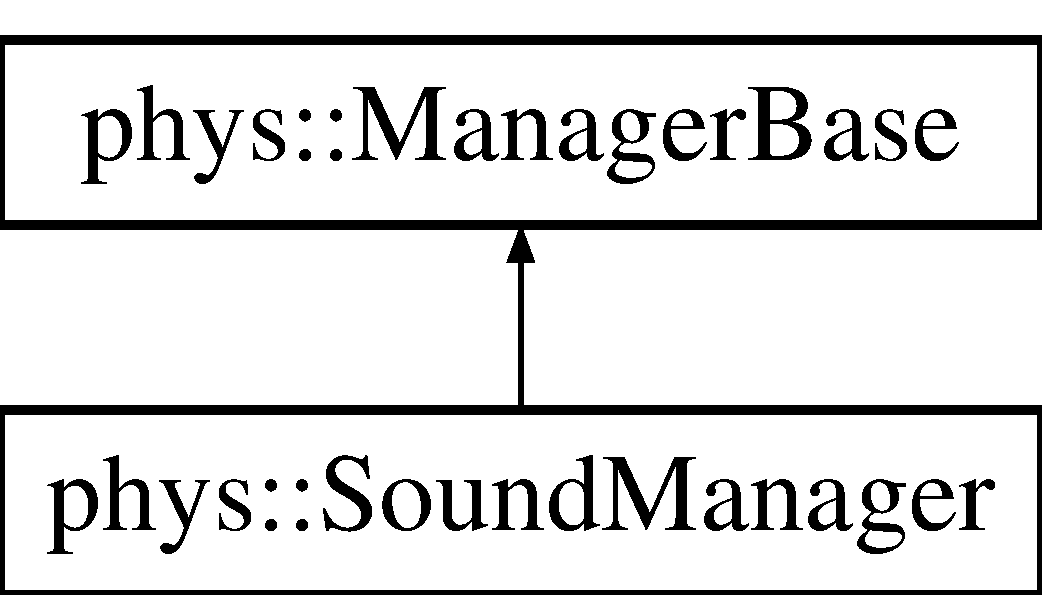
\includegraphics[height=2.000000cm]{d1/dc4/classphys_1_1SoundManager}
\end{center}
\end{figure}
\subsection*{Public Member Functions}
\begin{DoxyCompactItemize}
\item 
\hyperlink{classphys_1_1SoundManager_a42d41090652f8ef12d575d78881d6a05}{SoundManager} (bool DefaultSettings=true)
\begin{DoxyCompactList}\small\item\em Class Constructor. \item\end{DoxyCompactList}\item 
\hyperlink{classphys_1_1SoundManager_af557110e5f0eccc7be861f163e1670d0}{$\sim$SoundManager} ()
\begin{DoxyCompactList}\small\item\em Class Destructor. \item\end{DoxyCompactList}\item 
void \hyperlink{classphys_1_1SoundManager_ae6d3957f965b54e06ec540e903cec68d}{Initialize} ()
\begin{DoxyCompactList}\small\item\em Inherited Initializer. \item\end{DoxyCompactList}\item 
virtual void \hyperlink{classphys_1_1SoundManager_a577b228753ea19856b8476ab831e547e}{DoMainLoopItems} ()
\begin{DoxyCompactList}\small\item\em Empty MainLoopItems. \item\end{DoxyCompactList}\item 
void \hyperlink{classphys_1_1SoundManager_aa0fc07170611851f3fa888c8e28d99df}{InitializeManager} (\hyperlink{namespacephys_aa03900411993de7fbfec4789bc1d392e}{String} \&DeviceName, int OutputFrequency=-\/1, int EAXEffectSlots=4)
\begin{DoxyCompactList}\small\item\em Initializes the Manager. \item\end{DoxyCompactList}\item 
\hyperlink{classphys_1_1Sound}{Sound} $\ast$ \hyperlink{classphys_1_1SoundManager_ac9e68fef909b72110e9b68ff2674bcbb}{CreateSound} (\hyperlink{namespacephys_aa03900411993de7fbfec4789bc1d392e}{String} \&SoundName, \hyperlink{namespacephys_aa03900411993de7fbfec4789bc1d392e}{String} \&FilePath, bool Stream)
\begin{DoxyCompactList}\small\item\em Creates a sound instance from a file that can be used to play sounds. \item\end{DoxyCompactList}\item 
\hyperlink{classphys_1_1Sound}{Sound} $\ast$ \hyperlink{classphys_1_1SoundManager_aa039c3d7a5ee961be0934a58fd3826fa}{CreateSoundFromMemory} (\hyperlink{namespacephys_aa03900411993de7fbfec4789bc1d392e}{String} \&SoundName, const char $\ast$Data, int Size, \hyperlink{namespacephys_aa03900411993de7fbfec4789bc1d392e}{String} \&Extension)
\begin{DoxyCompactList}\small\item\em Creates a sound instance from a memory buffer. \item\end{DoxyCompactList}\item 
void \hyperlink{classphys_1_1SoundManager_a6a996829cab647ccf1ca401361af7167}{DestroySound} (\hyperlink{classphys_1_1Sound}{Sound} $\ast$SoundName)
\begin{DoxyCompactList}\small\item\em Deletes a \hyperlink{classphys_1_1Sound}{Sound}. \item\end{DoxyCompactList}\item 
\hyperlink{classphys_1_1Sound}{Sound} $\ast$ \hyperlink{classphys_1_1SoundManager_aa325440a688757ad74812b7f093e2423}{GetSoundByName} (\hyperlink{namespacephys_aa03900411993de7fbfec4789bc1d392e}{String} SoundName)
\begin{DoxyCompactList}\small\item\em Gets a sound by it's name. \item\end{DoxyCompactList}\item 
void \hyperlink{classphys_1_1SoundManager_a0f523240530abd5ab437c9eace78056a}{DestroyAllSounds} ()
\begin{DoxyCompactList}\small\item\em Deletes all stored sounds. \item\end{DoxyCompactList}\item 
\hyperlink{namespacephys_ab780c3162da5699fe421f3739ba03fc4}{SoundSet} $\ast$ \hyperlink{classphys_1_1SoundManager_afccb11a6f6d9aa9768a185febb0af45a}{CreateSoundSet} (\hyperlink{namespacephys_aa03900411993de7fbfec4789bc1d392e}{String} SoundSetName)
\begin{DoxyCompactList}\small\item\em Creates a sound set. \item\end{DoxyCompactList}\item 
\hyperlink{namespacephys_ab780c3162da5699fe421f3739ba03fc4}{SoundSet} $\ast$ \hyperlink{classphys_1_1SoundManager_a419edd2aed481ed7eff4beb11c9a6cf2}{GetSoundSet} (\hyperlink{namespacephys_aa03900411993de7fbfec4789bc1d392e}{String} SoundSetName)
\begin{DoxyCompactList}\small\item\em Gets an existing sound set. \item\end{DoxyCompactList}\item 
void \hyperlink{classphys_1_1SoundManager_a89c05a5628e187939ea30b0e4b149931}{AddSoundToSoundSet} (\hyperlink{namespacephys_aa03900411993de7fbfec4789bc1d392e}{String} SoundSetName, \hyperlink{classphys_1_1Sound}{Sound} $\ast$SoundInst)
\begin{DoxyCompactList}\small\item\em Add's a sound to the defined set. \item\end{DoxyCompactList}\item 
\hyperlink{namespacephys_aa03900411993de7fbfec4789bc1d392e}{String} \hyperlink{classphys_1_1SoundManager_a842f7cba6b12585bca77f642ecb8be79}{GetAvailableDeviceNameByIndex} (\hyperlink{namespacephys_a460f6bc24c8dd347b05e0366ae34f34a}{Whole} Index)
\begin{DoxyCompactList}\small\item\em Gets the name of an available device. \item\end{DoxyCompactList}\item 
\hyperlink{namespacephys_aa03900411993de7fbfec4789bc1d392e}{String} \hyperlink{classphys_1_1SoundManager_ac4814331683597034b26fac5c1c69bfa}{GetDefaultDeviceName} ()
\begin{DoxyCompactList}\small\item\em Gets the name of the default device. \item\end{DoxyCompactList}\item 
\hyperlink{namespacephys_a460f6bc24c8dd347b05e0366ae34f34a}{Whole} \hyperlink{classphys_1_1SoundManager_adb5717af71da8829600fd613a2ce615b}{GetAvailableDeviceCount} ()
\begin{DoxyCompactList}\small\item\em Gets the number of available devices. \item\end{DoxyCompactList}\item 
\hyperlink{classphys_1_1SoundListener}{SoundListener} $\ast$ \hyperlink{classphys_1_1SoundManager_af0c700e283c44c20466185e1150fc6a3}{GetListener} ()
\begin{DoxyCompactList}\small\item\em Retrieve's the listener for this sound manager. \item\end{DoxyCompactList}\item 
\hyperlink{classphys_1_1ManagerBase_aaa6ccddf23892eaccb898529414f80a5}{ManagerTypeName} \hyperlink{classphys_1_1SoundManager_a6815f78a6170b119e2d1d24e862ffbf8}{GetType} () const 
\begin{DoxyCompactList}\small\item\em Gets the manager type. \item\end{DoxyCompactList}\item 
std::stringstream $\ast$ \hyperlink{classphys_1_1SoundManager_a284fbc2fdbecdf66e717366b09e2c9da}{GetLogs} ()
\begin{DoxyCompactList}\small\item\em This gets the logs that the audio subystem creates. \item\end{DoxyCompactList}\item 
void \hyperlink{classphys_1_1SoundManager_acc3551bcda7b1c681d83d81cc25747ae}{ClearLogs} ()
\begin{DoxyCompactList}\small\item\em This empties logs that the audio subystem creates. \item\end{DoxyCompactList}\end{DoxyCompactItemize}
\subsection*{Protected Attributes}
\begin{DoxyCompactItemize}
\item 
\hypertarget{classphys_1_1SoundManager_a16bf0c35e031e2359d27c6b12536c98d}{
cAudio::IAudioManager $\ast$ {\bfseries AudioManager}}
\label{d1/dc4/classphys_1_1SoundManager_a16bf0c35e031e2359d27c6b12536c98d}

\item 
\hypertarget{classphys_1_1SoundManager_a7a8e89ec9886d28cf6331930b4269fb3}{
std::map$<$ \hyperlink{namespacephys_aa03900411993de7fbfec4789bc1d392e}{String}, \hyperlink{namespacephys_ab780c3162da5699fe421f3739ba03fc4}{SoundSet} $\ast$ $>$ {\bfseries SoundSets}}
\label{d1/dc4/classphys_1_1SoundManager_a7a8e89ec9886d28cf6331930b4269fb3}

\item 
\hypertarget{classphys_1_1SoundManager_a5b882ae37b8fbe843eee1f865be72a51}{
cAudio::IListener $\ast$ {\bfseries AudioListener}}
\label{d1/dc4/classphys_1_1SoundManager_a5b882ae37b8fbe843eee1f865be72a51}

\end{DoxyCompactItemize}


\subsection{Detailed Description}
This is simply a place for storing all the \hyperlink{classphys_1_1Sound}{Sound} utilities and functions. This is a place for loading, storing, and running sound files as necessary in a given game. 

Definition at line 69 of file soundmanager.h.



\subsection{Constructor \& Destructor Documentation}
\hypertarget{classphys_1_1SoundManager_a42d41090652f8ef12d575d78881d6a05}{
\index{phys::SoundManager@{phys::SoundManager}!SoundManager@{SoundManager}}
\index{SoundManager@{SoundManager}!phys::SoundManager@{phys::SoundManager}}
\subsubsection[{SoundManager}]{\setlength{\rightskip}{0pt plus 5cm}phys::SoundManager::SoundManager (
\begin{DoxyParamCaption}
\item[{bool}]{ DefaultSettings = {\ttfamily true}}
\end{DoxyParamCaption}
)}}
\label{d1/dc4/classphys_1_1SoundManager_a42d41090652f8ef12d575d78881d6a05}


Class Constructor. 

This is the class constructor. It gives you the option to start up the manager with default values if you choose. If not then you'll need to setup and initialize the manager yourself after it is constructed. 
\begin{DoxyParams}{Parameters}
\item[{\em DefaultSettings}]Whether or not to load default settings and initialize the manager immediately. \end{DoxyParams}


Definition at line 49 of file soundmanager.cpp.

\hypertarget{classphys_1_1SoundManager_af557110e5f0eccc7be861f163e1670d0}{
\index{phys::SoundManager@{phys::SoundManager}!$\sim$SoundManager@{$\sim$SoundManager}}
\index{$\sim$SoundManager@{$\sim$SoundManager}!phys::SoundManager@{phys::SoundManager}}
\subsubsection[{$\sim$SoundManager}]{\setlength{\rightskip}{0pt plus 5cm}phys::SoundManager::$\sim$SoundManager (
\begin{DoxyParamCaption}
{}
\end{DoxyParamCaption}
)}}
\label{d1/dc4/classphys_1_1SoundManager_af557110e5f0eccc7be861f163e1670d0}


Class Destructor. 

The class destructor. 

Definition at line 56 of file soundmanager.cpp.



\subsection{Member Function Documentation}
\hypertarget{classphys_1_1SoundManager_a89c05a5628e187939ea30b0e4b149931}{
\index{phys::SoundManager@{phys::SoundManager}!AddSoundToSoundSet@{AddSoundToSoundSet}}
\index{AddSoundToSoundSet@{AddSoundToSoundSet}!phys::SoundManager@{phys::SoundManager}}
\subsubsection[{AddSoundToSoundSet}]{\setlength{\rightskip}{0pt plus 5cm}void phys::SoundManager::AddSoundToSoundSet (
\begin{DoxyParamCaption}
\item[{{\bf String}}]{ SoundSetName, }
\item[{{\bf Sound} $\ast$}]{ SoundInst}
\end{DoxyParamCaption}
)}}
\label{d1/dc4/classphys_1_1SoundManager_a89c05a5628e187939ea30b0e4b149931}


Add's a sound to the defined set. 

This function will add a sound instance to a created sound set. 
\begin{DoxyParams}{Parameters}
\item[{\em SoundName}]The sound instance to be added. \end{DoxyParams}


Definition at line 155 of file soundmanager.cpp.

\hypertarget{classphys_1_1SoundManager_acc3551bcda7b1c681d83d81cc25747ae}{
\index{phys::SoundManager@{phys::SoundManager}!ClearLogs@{ClearLogs}}
\index{ClearLogs@{ClearLogs}!phys::SoundManager@{phys::SoundManager}}
\subsubsection[{ClearLogs}]{\setlength{\rightskip}{0pt plus 5cm}void phys::SoundManager::ClearLogs (
\begin{DoxyParamCaption}
{}
\end{DoxyParamCaption}
)}}
\label{d1/dc4/classphys_1_1SoundManager_acc3551bcda7b1c681d83d81cc25747ae}


This empties logs that the audio subystem creates. 

Internally the Physgame engine currently uses cAudio to process 3d sound. It has it's own logging system that we have customized to work with our logger. This clears that data allow us to work with it as we need 

Definition at line 194 of file soundmanager.cpp.

\hypertarget{classphys_1_1SoundManager_ac9e68fef909b72110e9b68ff2674bcbb}{
\index{phys::SoundManager@{phys::SoundManager}!CreateSound@{CreateSound}}
\index{CreateSound@{CreateSound}!phys::SoundManager@{phys::SoundManager}}
\subsubsection[{CreateSound}]{\setlength{\rightskip}{0pt plus 5cm}{\bf Sound} $\ast$ phys::SoundManager::CreateSound (
\begin{DoxyParamCaption}
\item[{{\bf String} \&}]{ SoundName, }
\item[{{\bf String} \&}]{ FilePath, }
\item[{bool}]{ Stream}
\end{DoxyParamCaption}
)}}
\label{d1/dc4/classphys_1_1SoundManager_ac9e68fef909b72110e9b68ff2674bcbb}


Creates a sound instance from a file that can be used to play sounds. 

This function will create a \hyperlink{classphys_1_1Sound}{Sound} from a file and returns a pointer to that \hyperlink{classphys_1_1Sound}{Sound}. You can also specify if you want the sound to be streamed from the disk so that it doesn't have to load the entire song from disk first. 
\begin{DoxyParams}{Parameters}
\item[{\em SoundName}]The name of the \hyperlink{classphys_1_1Sound}{Sound} instance. \item[{\em FilePath}]The path to the file AND the name of the file. \item[{\em Stream}]Whether or not to stream the audio from the disk. Otherwise it has be completely loaded into memory before it can be used. \end{DoxyParams}
\begin{DoxyReturn}{Returns}
Returns a pointer to the \hyperlink{classphys_1_1Sound}{Sound} Instance that was created. 
\end{DoxyReturn}


Definition at line 74 of file soundmanager.cpp.

\hypertarget{classphys_1_1SoundManager_aa039c3d7a5ee961be0934a58fd3826fa}{
\index{phys::SoundManager@{phys::SoundManager}!CreateSoundFromMemory@{CreateSoundFromMemory}}
\index{CreateSoundFromMemory@{CreateSoundFromMemory}!phys::SoundManager@{phys::SoundManager}}
\subsubsection[{CreateSoundFromMemory}]{\setlength{\rightskip}{0pt plus 5cm}{\bf Sound} $\ast$ phys::SoundManager::CreateSoundFromMemory (
\begin{DoxyParamCaption}
\item[{{\bf String} \&}]{ SoundName, }
\item[{const char $\ast$}]{ Data, }
\item[{int}]{ Size, }
\item[{{\bf String} \&}]{ Extension}
\end{DoxyParamCaption}
)}}
\label{d1/dc4/classphys_1_1SoundManager_aa039c3d7a5ee961be0934a58fd3826fa}


Creates a sound instance from a memory buffer. 

This function allows you to create a sound instance from a sound that is already loaded into memory. 
\begin{DoxyParams}{Parameters}
\item[{\em SoundName}]The name of the sound instance. \item[{\em Data}]Pointer to the char array (buffer). \item[{\em Size}]Size of the char array (buffer). \item[{\em Extension}]The extension of the file used to load that sound (wav, ogg). \end{DoxyParams}
\begin{DoxyReturn}{Returns}
Returns a pointer to the \hyperlink{classphys_1_1Sound}{Sound} Instance that was created. 
\end{DoxyReturn}


Definition at line 86 of file soundmanager.cpp.

\hypertarget{classphys_1_1SoundManager_afccb11a6f6d9aa9768a185febb0af45a}{
\index{phys::SoundManager@{phys::SoundManager}!CreateSoundSet@{CreateSoundSet}}
\index{CreateSoundSet@{CreateSoundSet}!phys::SoundManager@{phys::SoundManager}}
\subsubsection[{CreateSoundSet}]{\setlength{\rightskip}{0pt plus 5cm}{\bf SoundSet} $\ast$ phys::SoundManager::CreateSoundSet (
\begin{DoxyParamCaption}
\item[{{\bf String}}]{ SoundSetName}
\end{DoxyParamCaption}
)}}
\label{d1/dc4/classphys_1_1SoundManager_afccb11a6f6d9aa9768a185febb0af45a}


Creates a sound set. 

This function will create a sound set vector you can use to store similiar sound instances. 
\begin{DoxyParams}{Parameters}
\item[{\em SoundSetName}]The name you wish the sound set to have. \end{DoxyParams}
\begin{DoxyReturn}{Returns}
Returns a pointer to the created Vector. 
\end{DoxyReturn}


Definition at line 142 of file soundmanager.cpp.

\hypertarget{classphys_1_1SoundManager_a0f523240530abd5ab437c9eace78056a}{
\index{phys::SoundManager@{phys::SoundManager}!DestroyAllSounds@{DestroyAllSounds}}
\index{DestroyAllSounds@{DestroyAllSounds}!phys::SoundManager@{phys::SoundManager}}
\subsubsection[{DestroyAllSounds}]{\setlength{\rightskip}{0pt plus 5cm}void phys::SoundManager::DestroyAllSounds (
\begin{DoxyParamCaption}
{}
\end{DoxyParamCaption}
)}}
\label{d1/dc4/classphys_1_1SoundManager_a0f523240530abd5ab437c9eace78056a}


Deletes all stored sounds. 

This function will delete every \hyperlink{classphys_1_1Sound}{Sound} that is stored in the manager. 

Definition at line 126 of file soundmanager.cpp.

\hypertarget{classphys_1_1SoundManager_a6a996829cab647ccf1ca401361af7167}{
\index{phys::SoundManager@{phys::SoundManager}!DestroySound@{DestroySound}}
\index{DestroySound@{DestroySound}!phys::SoundManager@{phys::SoundManager}}
\subsubsection[{DestroySound}]{\setlength{\rightskip}{0pt plus 5cm}void phys::SoundManager::DestroySound (
\begin{DoxyParamCaption}
\item[{{\bf Sound} $\ast$}]{ SoundName}
\end{DoxyParamCaption}
)}}
\label{d1/dc4/classphys_1_1SoundManager_a6a996829cab647ccf1ca401361af7167}


Deletes a \hyperlink{classphys_1_1Sound}{Sound}. 

Deletes a single \hyperlink{classphys_1_1Sound}{Sound} via a pointer. 
\begin{DoxyParams}{Parameters}
\item[{\em SoundName}]A pointer to the \hyperlink{classphys_1_1Sound}{Sound} you want deleted. \end{DoxyParams}


Definition at line 121 of file soundmanager.cpp.

\hypertarget{classphys_1_1SoundManager_a577b228753ea19856b8476ab831e547e}{
\index{phys::SoundManager@{phys::SoundManager}!DoMainLoopItems@{DoMainLoopItems}}
\index{DoMainLoopItems@{DoMainLoopItems}!phys::SoundManager@{phys::SoundManager}}
\subsubsection[{DoMainLoopItems}]{\setlength{\rightskip}{0pt plus 5cm}void phys::SoundManager::DoMainLoopItems (
\begin{DoxyParamCaption}
{}
\end{DoxyParamCaption}
)\hspace{0.3cm}{\ttfamily  \mbox{[}virtual\mbox{]}}}}
\label{d1/dc4/classphys_1_1SoundManager_a577b228753ea19856b8476ab831e547e}


Empty MainLoopItems. 

This class implements this for the sake of entension and compatibility this function does nothing 

Implements \hyperlink{classphys_1_1ManagerBase_aa9e13a3f7c398b708f0f242610b5abf7}{phys::ManagerBase}.



Definition at line 65 of file soundmanager.cpp.

\hypertarget{classphys_1_1SoundManager_adb5717af71da8829600fd613a2ce615b}{
\index{phys::SoundManager@{phys::SoundManager}!GetAvailableDeviceCount@{GetAvailableDeviceCount}}
\index{GetAvailableDeviceCount@{GetAvailableDeviceCount}!phys::SoundManager@{phys::SoundManager}}
\subsubsection[{GetAvailableDeviceCount}]{\setlength{\rightskip}{0pt plus 5cm}{\bf Whole} phys::SoundManager::GetAvailableDeviceCount (
\begin{DoxyParamCaption}
{}
\end{DoxyParamCaption}
)}}
\label{d1/dc4/classphys_1_1SoundManager_adb5717af71da8829600fd613a2ce615b}


Gets the number of available devices. 

This function will return the total number of available devices, including the default. \begin{DoxyReturn}{Returns}
Returns the number of available devices. 
\end{DoxyReturn}


Definition at line 175 of file soundmanager.cpp.

\hypertarget{classphys_1_1SoundManager_a842f7cba6b12585bca77f642ecb8be79}{
\index{phys::SoundManager@{phys::SoundManager}!GetAvailableDeviceNameByIndex@{GetAvailableDeviceNameByIndex}}
\index{GetAvailableDeviceNameByIndex@{GetAvailableDeviceNameByIndex}!phys::SoundManager@{phys::SoundManager}}
\subsubsection[{GetAvailableDeviceNameByIndex}]{\setlength{\rightskip}{0pt plus 5cm}{\bf String} phys::SoundManager::GetAvailableDeviceNameByIndex (
\begin{DoxyParamCaption}
\item[{{\bf Whole}}]{ Index}
\end{DoxyParamCaption}
)}}
\label{d1/dc4/classphys_1_1SoundManager_a842f7cba6b12585bca77f642ecb8be79}


Gets the name of an available device. 

This function will retrieve the name of a device by it's index on the sound managers device list. 
\begin{DoxyParams}{Parameters}
\item[{\em Index}]The position on the device list you wish to access the name of. \end{DoxyParams}
\begin{DoxyReturn}{Returns}
Returns the name of the device. 
\end{DoxyReturn}


Definition at line 161 of file soundmanager.cpp.

\hypertarget{classphys_1_1SoundManager_ac4814331683597034b26fac5c1c69bfa}{
\index{phys::SoundManager@{phys::SoundManager}!GetDefaultDeviceName@{GetDefaultDeviceName}}
\index{GetDefaultDeviceName@{GetDefaultDeviceName}!phys::SoundManager@{phys::SoundManager}}
\subsubsection[{GetDefaultDeviceName}]{\setlength{\rightskip}{0pt plus 5cm}{\bf String} phys::SoundManager::GetDefaultDeviceName (
\begin{DoxyParamCaption}
{}
\end{DoxyParamCaption}
)}}
\label{d1/dc4/classphys_1_1SoundManager_ac4814331683597034b26fac5c1c69bfa}


Gets the name of the default device. 

This function will return the name of the system default device. \begin{DoxyReturn}{Returns}
Returns the name of the default device. 
\end{DoxyReturn}


Definition at line 168 of file soundmanager.cpp.

\hypertarget{classphys_1_1SoundManager_af0c700e283c44c20466185e1150fc6a3}{
\index{phys::SoundManager@{phys::SoundManager}!GetListener@{GetListener}}
\index{GetListener@{GetListener}!phys::SoundManager@{phys::SoundManager}}
\subsubsection[{GetListener}]{\setlength{\rightskip}{0pt plus 5cm}{\bf SoundListener} $\ast$ phys::SoundManager::GetListener (
\begin{DoxyParamCaption}
{}
\end{DoxyParamCaption}
)}}
\label{d1/dc4/classphys_1_1SoundManager_af0c700e283c44c20466185e1150fc6a3}


Retrieve's the listener for this sound manager. 

This function will return the listener for this manager which can be used to help create 3D sound. \begin{DoxyReturn}{Returns}
Returns a pointer to the managers \hyperlink{classphys_1_1Sound}{Sound} Listener. 
\end{DoxyReturn}


Definition at line 180 of file soundmanager.cpp.

\hypertarget{classphys_1_1SoundManager_a284fbc2fdbecdf66e717366b09e2c9da}{
\index{phys::SoundManager@{phys::SoundManager}!GetLogs@{GetLogs}}
\index{GetLogs@{GetLogs}!phys::SoundManager@{phys::SoundManager}}
\subsubsection[{GetLogs}]{\setlength{\rightskip}{0pt plus 5cm}std::stringstream $\ast$ phys::SoundManager::GetLogs (
\begin{DoxyParamCaption}
{}
\end{DoxyParamCaption}
)}}
\label{d1/dc4/classphys_1_1SoundManager_a284fbc2fdbecdf66e717366b09e2c9da}


This gets the logs that the audio subystem creates. 

Internally the Physgame engine currently uses cAudio to process 3d sound. It has it's own logging system that we have customized to work with our logger. \begin{DoxyReturn}{Returns}
This gets the log of what actions the audio system has performed 
\end{DoxyReturn}


Definition at line 189 of file soundmanager.cpp.

\hypertarget{classphys_1_1SoundManager_aa325440a688757ad74812b7f093e2423}{
\index{phys::SoundManager@{phys::SoundManager}!GetSoundByName@{GetSoundByName}}
\index{GetSoundByName@{GetSoundByName}!phys::SoundManager@{phys::SoundManager}}
\subsubsection[{GetSoundByName}]{\setlength{\rightskip}{0pt plus 5cm}{\bf Sound} $\ast$ phys::SoundManager::GetSoundByName (
\begin{DoxyParamCaption}
\item[{{\bf String}}]{ SoundName}
\end{DoxyParamCaption}
)}}
\label{d1/dc4/classphys_1_1SoundManager_aa325440a688757ad74812b7f093e2423}


Gets a sound by it's name. 

This function will find and return the sound with the speicified name. \begin{DoxyReturn}{Returns}
Returns a pointer to the specified sound. 
\end{DoxyReturn}


Definition at line 131 of file soundmanager.cpp.

\hypertarget{classphys_1_1SoundManager_a419edd2aed481ed7eff4beb11c9a6cf2}{
\index{phys::SoundManager@{phys::SoundManager}!GetSoundSet@{GetSoundSet}}
\index{GetSoundSet@{GetSoundSet}!phys::SoundManager@{phys::SoundManager}}
\subsubsection[{GetSoundSet}]{\setlength{\rightskip}{0pt plus 5cm}{\bf SoundSet} $\ast$ phys::SoundManager::GetSoundSet (
\begin{DoxyParamCaption}
\item[{{\bf String}}]{ SoundSetName}
\end{DoxyParamCaption}
)}}
\label{d1/dc4/classphys_1_1SoundManager_a419edd2aed481ed7eff4beb11c9a6cf2}


Gets an existing sound set. 

This function will find the specified sound set and return a pointer to it. 
\begin{DoxyParams}{Parameters}
\item[{\em SoundSetName}]The name of the sound set to retrieve. \end{DoxyParams}
\begin{DoxyReturn}{Returns}
Returns a pointer to the named Vector. 
\end{DoxyReturn}


Definition at line 149 of file soundmanager.cpp.

\hypertarget{classphys_1_1SoundManager_a6815f78a6170b119e2d1d24e862ffbf8}{
\index{phys::SoundManager@{phys::SoundManager}!GetType@{GetType}}
\index{GetType@{GetType}!phys::SoundManager@{phys::SoundManager}}
\subsubsection[{GetType}]{\setlength{\rightskip}{0pt plus 5cm}{\bf ManagerBase::ManagerTypeName} phys::SoundManager::GetType (
\begin{DoxyParamCaption}
{}
\end{DoxyParamCaption}
) const\hspace{0.3cm}{\ttfamily  \mbox{[}virtual\mbox{]}}}}
\label{d1/dc4/classphys_1_1SoundManager_a6815f78a6170b119e2d1d24e862ffbf8}


Gets the manager type. 

Gets the type of manager that this is. \begin{DoxyReturn}{Returns}
Returns the manager type. 
\end{DoxyReturn}


Implements \hyperlink{classphys_1_1ManagerBase_aff400b6599db635e24796d8221e9a0e3}{phys::ManagerBase}.



Definition at line 186 of file soundmanager.cpp.

\hypertarget{classphys_1_1SoundManager_ae6d3957f965b54e06ec540e903cec68d}{
\index{phys::SoundManager@{phys::SoundManager}!Initialize@{Initialize}}
\index{Initialize@{Initialize}!phys::SoundManager@{phys::SoundManager}}
\subsubsection[{Initialize}]{\setlength{\rightskip}{0pt plus 5cm}void phys::SoundManager::Initialize (
\begin{DoxyParamCaption}
{}
\end{DoxyParamCaption}
)\hspace{0.3cm}{\ttfamily  \mbox{[}virtual\mbox{]}}}}
\label{d1/dc4/classphys_1_1SoundManager_ae6d3957f965b54e06ec540e903cec68d}


Inherited Initializer. 

Written to allow the class to compile, this currently does nothing, but could be used to run code Use \hyperlink{classphys_1_1SoundManager_aa0fc07170611851f3fa888c8e28d99df}{InitializeManager()} instead. 

Implements \hyperlink{classphys_1_1ManagerBase_a57dd8e54e767427d5bdcc86dc66d73ed}{phys::ManagerBase}.



Definition at line 61 of file soundmanager.cpp.

\hypertarget{classphys_1_1SoundManager_aa0fc07170611851f3fa888c8e28d99df}{
\index{phys::SoundManager@{phys::SoundManager}!InitializeManager@{InitializeManager}}
\index{InitializeManager@{InitializeManager}!phys::SoundManager@{phys::SoundManager}}
\subsubsection[{InitializeManager}]{\setlength{\rightskip}{0pt plus 5cm}void phys::SoundManager::InitializeManager (
\begin{DoxyParamCaption}
\item[{{\bf String} \&}]{ DeviceName, }
\item[{int}]{ OutputFrequency = {\ttfamily -\/1}, }
\item[{int}]{ EAXEffectSlots = {\ttfamily 4}}
\end{DoxyParamCaption}
)}}
\label{d1/dc4/classphys_1_1SoundManager_aa0fc07170611851f3fa888c8e28d99df}


Initializes the Manager. 

This function will initialize the manager using the device and parameters provided. You need to call this function if you passed false into the sound manager constructor before you can use the manager. 
\begin{DoxyParams}{Parameters}
\item[{\em DeviceName}]The name of the device you wish to have this manager interface with/use. \item[{\em OutputFrequency}]Frequency of the output audio, -\/1 for the devices default. \item[{\em EAXEffectSlots}]The number of effects per sound allowed to be applied. \end{DoxyParams}


Definition at line 69 of file soundmanager.cpp.



The documentation for this class was generated from the following files:\begin{DoxyCompactItemize}
\item 
soundmanager.h\item 
soundmanager.cpp\end{DoxyCompactItemize}

\hypertarget{classphys_1_1TestAE}{
\section{phys::TestAE Class Reference}
\label{d1/dca/classphys_1_1TestAE}\index{phys::TestAE@{phys::TestAE}}
}


This is a dummy class to test if the AE field works. Details will be output to the log.  




{\ttfamily \#include $<$areaeffect.h$>$}

Inheritance diagram for phys::TestAE:\begin{figure}[H]
\begin{center}
\leavevmode
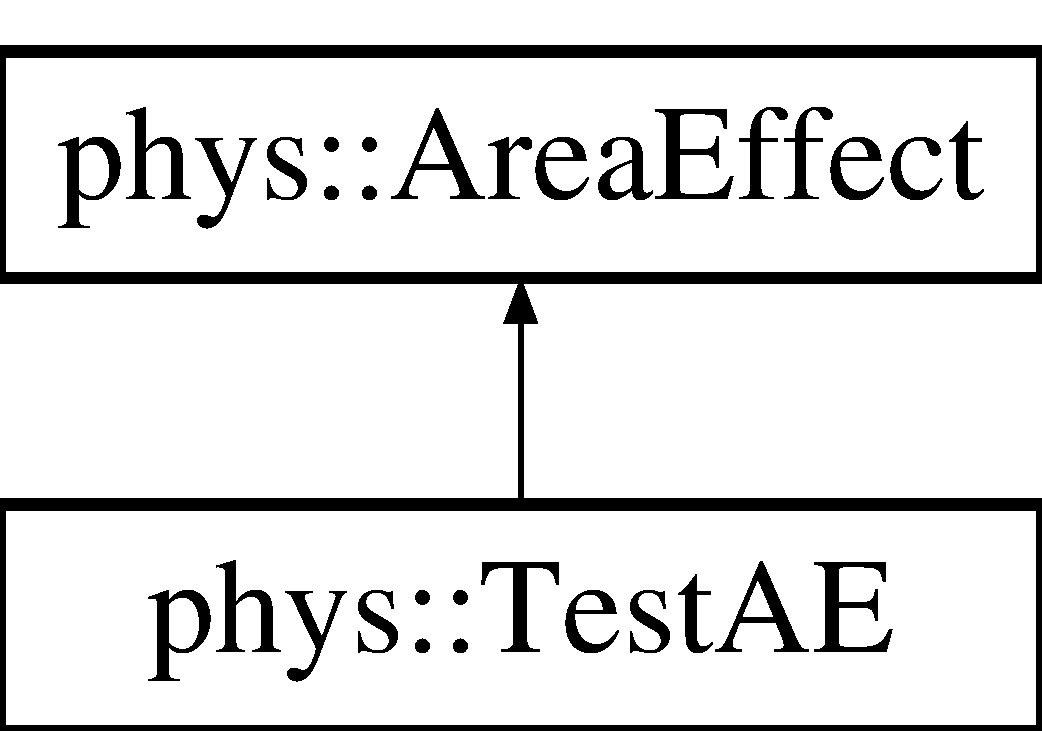
\includegraphics[height=2.000000cm]{d1/dca/classphys_1_1TestAE}
\end{center}
\end{figure}
\subsection*{Public Member Functions}
\begin{DoxyCompactItemize}
\item 
\hyperlink{classphys_1_1TestAE_a851bf73722a9b3a3886e1dbf4600861c}{TestAE} (const \hyperlink{namespacephys_aa03900411993de7fbfec4789bc1d392e}{String} \&name, \hyperlink{classphys_1_1Vector3}{Vector3} Location)
\begin{DoxyCompactList}\small\item\em Constructor. \item\end{DoxyCompactList}\item 
\hyperlink{classphys_1_1TestAE_aa3ceb77df713b5cafa97495de61e4b0a}{$\sim$TestAE} ()
\begin{DoxyCompactList}\small\item\em Destructor. \item\end{DoxyCompactList}\item 
virtual void \hyperlink{classphys_1_1TestAE_a191c60dbfa277e850ea392d9ab774c42}{ApplyEffect} ()
\begin{DoxyCompactList}\small\item\em Applies the effect this field has to object inside. \item\end{DoxyCompactList}\end{DoxyCompactItemize}


\subsection{Detailed Description}
This is a dummy class to test if the AE field works. Details will be output to the log. 

Definition at line 233 of file areaeffect.h.



\subsection{Constructor \& Destructor Documentation}
\hypertarget{classphys_1_1TestAE_a851bf73722a9b3a3886e1dbf4600861c}{
\index{phys::TestAE@{phys::TestAE}!TestAE@{TestAE}}
\index{TestAE@{TestAE}!phys::TestAE@{phys::TestAE}}
\subsubsection[{TestAE}]{\setlength{\rightskip}{0pt plus 5cm}phys::TestAE::TestAE (
\begin{DoxyParamCaption}
\item[{const {\bf String} \&}]{ name, }
\item[{{\bf Vector3}}]{ Location}
\end{DoxyParamCaption}
)}}
\label{d1/dca/classphys_1_1TestAE_a851bf73722a9b3a3886e1dbf4600861c}


Constructor. 

Basic initialization constructor. 
\begin{DoxyParams}{Parameters}
\item[{\em name}]The name of the field. \item[{\em Location}]The location of the AE field. \end{DoxyParams}


Definition at line 469 of file areaeffect.cpp.

\hypertarget{classphys_1_1TestAE_aa3ceb77df713b5cafa97495de61e4b0a}{
\index{phys::TestAE@{phys::TestAE}!$\sim$TestAE@{$\sim$TestAE}}
\index{$\sim$TestAE@{$\sim$TestAE}!phys::TestAE@{phys::TestAE}}
\subsubsection[{$\sim$TestAE}]{\setlength{\rightskip}{0pt plus 5cm}phys::TestAE::$\sim$TestAE (
\begin{DoxyParamCaption}
{}
\end{DoxyParamCaption}
)}}
\label{d1/dca/classphys_1_1TestAE_aa3ceb77df713b5cafa97495de61e4b0a}


Destructor. 

Class destructor. 

Definition at line 473 of file areaeffect.cpp.



\subsection{Member Function Documentation}
\hypertarget{classphys_1_1TestAE_a191c60dbfa277e850ea392d9ab774c42}{
\index{phys::TestAE@{phys::TestAE}!ApplyEffect@{ApplyEffect}}
\index{ApplyEffect@{ApplyEffect}!phys::TestAE@{phys::TestAE}}
\subsubsection[{ApplyEffect}]{\setlength{\rightskip}{0pt plus 5cm}void phys::TestAE::ApplyEffect (
\begin{DoxyParamCaption}
{}
\end{DoxyParamCaption}
)\hspace{0.3cm}{\ttfamily  \mbox{[}virtual\mbox{]}}}}
\label{d1/dca/classphys_1_1TestAE_a191c60dbfa277e850ea392d9ab774c42}


Applies the effect this field has to object inside. 

This function defines the behavior for the class. 

Implements \hyperlink{classphys_1_1AreaEffect_a3b285ecfcf9c9200662d510e48dd222a}{phys::AreaEffect}.



Definition at line 477 of file areaeffect.cpp.



The documentation for this class was generated from the following files:\begin{DoxyCompactItemize}
\item 
areaeffect.h\item 
areaeffect.cpp\end{DoxyCompactItemize}

\hypertarget{classphys_1_1UI_1_1TextButton}{
\section{phys::UI::TextButton Class Reference}
\label{df/d03/classphys_1_1UI_1_1TextButton}\index{phys::UI::TextButton@{phys::UI::TextButton}}
}


This is a button class that provides text capabilities.  




{\ttfamily \#include $<$uitextbutton.h$>$}

Inheritance diagram for phys::UI::TextButton:\begin{figure}[H]
\begin{center}
\leavevmode
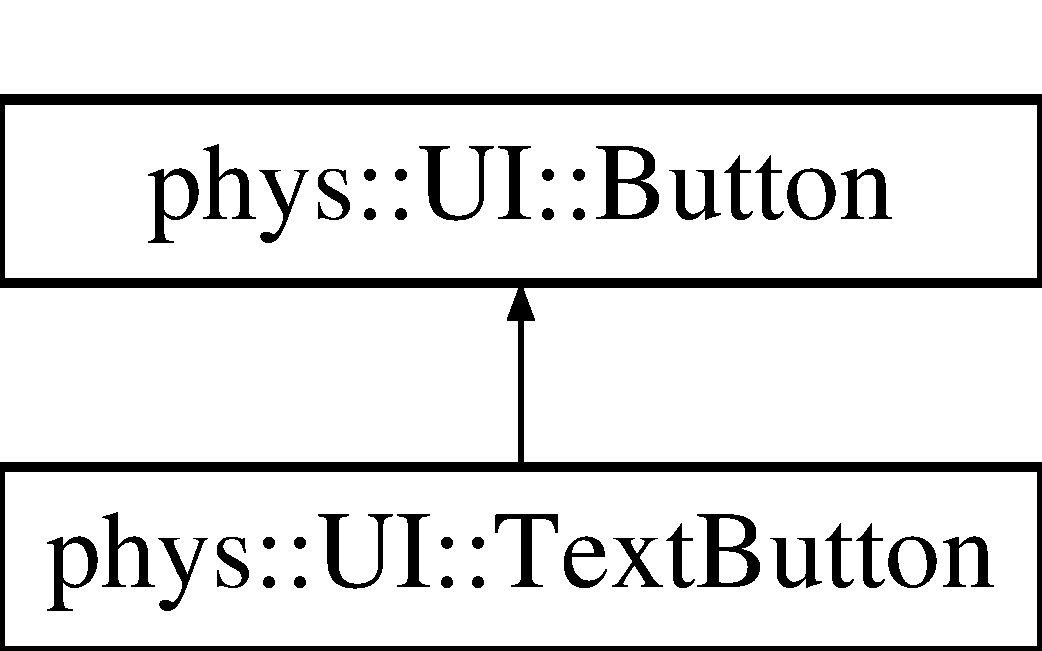
\includegraphics[height=2.000000cm]{df/d03/classphys_1_1UI_1_1TextButton}
\end{center}
\end{figure}
\subsection*{Public Member Functions}
\begin{DoxyCompactItemize}
\item 
\hyperlink{classphys_1_1UI_1_1TextButton_a319fd053824be479335d15df5f21131f}{TextButton} (\hyperlink{namespacephys_a5ce5049f8b4bf88d6413c47b504ebb31}{ConstString} \&name, const \hyperlink{classphys_1_1Vector2}{Vector2} Position, const \hyperlink{classphys_1_1Vector2}{Vector2} Size, const \hyperlink{namespacephys_a460f6bc24c8dd347b05e0366ae34f34a}{Whole} Glyph, \hyperlink{namespacephys_aa03900411993de7fbfec4789bc1d392e}{String} Text, \hyperlink{classphys_1_1UILayer}{UILayer} $\ast$Layer)
\begin{DoxyCompactList}\small\item\em Internal constructor. \item\end{DoxyCompactList}\item 
\hypertarget{classphys_1_1UI_1_1TextButton_a1f28489fee45ee8ce7e1b0aea0f249a1}{
\hyperlink{classphys_1_1UI_1_1TextButton_a1f28489fee45ee8ce7e1b0aea0f249a1}{$\sim$TextButton} ()}
\label{df/d03/classphys_1_1UI_1_1TextButton_a1f28489fee45ee8ce7e1b0aea0f249a1}

\begin{DoxyCompactList}\small\item\em Class destructor. \item\end{DoxyCompactList}\item 
virtual void \hyperlink{classphys_1_1UI_1_1TextButton_a07e030ef92f314b1eff663cbc1712d42}{SetVisible} (bool Visible)
\begin{DoxyCompactList}\small\item\em Sets the visibility of this button. \item\end{DoxyCompactList}\item 
virtual bool \hyperlink{classphys_1_1UI_1_1TextButton_a505167a00d343d704df1f759cd12ed1e}{IsVisible} ()
\begin{DoxyCompactList}\small\item\em Gets the visibility of this button. \item\end{DoxyCompactList}\item 
\hypertarget{classphys_1_1UI_1_1TextButton_add95c812af6ef7584a2d515a33bac72b}{
virtual void \hyperlink{classphys_1_1UI_1_1TextButton_add95c812af6ef7584a2d515a33bac72b}{Show} ()}
\label{df/d03/classphys_1_1UI_1_1TextButton_add95c812af6ef7584a2d515a33bac72b}

\begin{DoxyCompactList}\small\item\em Forces this button to be shown. \item\end{DoxyCompactList}\item 
\hypertarget{classphys_1_1UI_1_1TextButton_aef823890ba8c829183f1b618473c1bac}{
virtual void \hyperlink{classphys_1_1UI_1_1TextButton_aef823890ba8c829183f1b618473c1bac}{Hide} ()}
\label{df/d03/classphys_1_1UI_1_1TextButton_aef823890ba8c829183f1b618473c1bac}

\begin{DoxyCompactList}\small\item\em Forces this button to hide. \item\end{DoxyCompactList}\item 
virtual void \hyperlink{classphys_1_1UI_1_1TextButton_ae66f149489c4215963dc5b853c838c50}{SetText} (\hyperlink{namespacephys_a5ce5049f8b4bf88d6413c47b504ebb31}{ConstString} \&Text)
\begin{DoxyCompactList}\small\item\em Sets the text displayed within the button. \item\end{DoxyCompactList}\item 
virtual \hyperlink{namespacephys_aa03900411993de7fbfec4789bc1d392e}{String} \hyperlink{classphys_1_1UI_1_1TextButton_a8dc28f2fa610dc9bb72e5886613996bd}{GetText} ()
\begin{DoxyCompactList}\small\item\em Gets the text displayed within the button. \item\end{DoxyCompactList}\item 
virtual void \hyperlink{classphys_1_1UI_1_1TextButton_a71a64810f262725992dbeec194e8497c}{HorizontallyAlign} (UI::TextHorizontalAlign Align)
\begin{DoxyCompactList}\small\item\em Aligns the text of the button. \item\end{DoxyCompactList}\item 
virtual void \hyperlink{classphys_1_1UI_1_1TextButton_a7319f855026794c9c42f292093d1351f}{VerticallyAlign} (UI::TextVerticalAlign Align)
\begin{DoxyCompactList}\small\item\em Aligns the text of the button. \item\end{DoxyCompactList}\item 
virtual void \hyperlink{classphys_1_1UI_1_1TextButton_acf40fd3a8382cdfc959d078e99f6ff0b}{SetPosition} (const \hyperlink{classphys_1_1Vector2}{Vector2} Position)
\begin{DoxyCompactList}\small\item\em Sets the relative top left position of this button. \item\end{DoxyCompactList}\item 
virtual \hyperlink{classphys_1_1Vector2}{Vector2} \hyperlink{classphys_1_1UI_1_1TextButton_a09768e0666a109b7d35fd8b78240cfd3}{GetPosition} ()
\begin{DoxyCompactList}\small\item\em Gets the relative top left position of this button. \item\end{DoxyCompactList}\item 
virtual void \hyperlink{classphys_1_1UI_1_1TextButton_a717a2a7fdcf625e833764381989c4b56}{SetActualPosition} (const \hyperlink{classphys_1_1Vector2}{Vector2} Position)
\begin{DoxyCompactList}\small\item\em Sets the top left position of this button in pixels. \item\end{DoxyCompactList}\item 
virtual \hyperlink{classphys_1_1Vector2}{Vector2} \hyperlink{classphys_1_1UI_1_1TextButton_ab406bec58bf6244c3e867fefd19d4d7f}{GetActualPosition} ()
\begin{DoxyCompactList}\small\item\em Gets the top left position of this button in pixels. \item\end{DoxyCompactList}\item 
virtual void \hyperlink{classphys_1_1UI_1_1TextButton_a7ed2a635d23906fcf1844e75018e20de}{SetSize} (const \hyperlink{classphys_1_1Vector2}{Vector2} Size)
\begin{DoxyCompactList}\small\item\em Sets the relative size of this button. \item\end{DoxyCompactList}\item 
virtual \hyperlink{classphys_1_1Vector2}{Vector2} \hyperlink{classphys_1_1UI_1_1TextButton_a21f1ff24070711e5a42eae4eb54d02d6}{GetSize} ()
\begin{DoxyCompactList}\small\item\em Gets the relative size of this button. \item\end{DoxyCompactList}\item 
virtual void \hyperlink{classphys_1_1UI_1_1TextButton_a7ed2be5c895c7fe01d7650746ccc57e9}{SetActualSize} (const \hyperlink{classphys_1_1Vector2}{Vector2} Size)
\begin{DoxyCompactList}\small\item\em Sets the size of this button in pixels. \item\end{DoxyCompactList}\item 
virtual \hyperlink{classphys_1_1Vector2}{Vector2} \hyperlink{classphys_1_1UI_1_1TextButton_a062b31c199f875d4f825f6be1d11fb55}{GetActualSize} ()
\begin{DoxyCompactList}\small\item\em Gets the size of this button in pixels. \item\end{DoxyCompactList}\item 
virtual void \hyperlink{classphys_1_1UI_1_1TextButton_a7d4e22acd792b10f2f7986d8f449ec16}{SetRenderPriority} (UI::RenderPriority Priority)
\begin{DoxyCompactList}\small\item\em Sets the priority this button should be rendered with. \item\end{DoxyCompactList}\item 
virtual UI::RenderPriority \hyperlink{classphys_1_1UI_1_1TextButton_ad339621af6e73ff9702c0dd4cdadbb73}{GetRenderPriority} ()
\begin{DoxyCompactList}\small\item\em Gets the priority this button should be rendered with. \item\end{DoxyCompactList}\end{DoxyCompactItemize}
\subsection*{Protected Attributes}
\begin{DoxyCompactItemize}
\item 
\hypertarget{classphys_1_1UI_1_1TextButton_a33fe39747602f948b462e008cb75bb5e}{
Gorilla::Caption $\ast$ {\bfseries GorillaButton}}
\label{df/d03/classphys_1_1UI_1_1TextButton_a33fe39747602f948b462e008cb75bb5e}

\end{DoxyCompactItemize}


\subsection{Detailed Description}
This is a button class that provides text capabilities. 

Definition at line 57 of file uitextbutton.h.



\subsection{Constructor \& Destructor Documentation}
\hypertarget{classphys_1_1UI_1_1TextButton_a319fd053824be479335d15df5f21131f}{
\index{phys::UI::TextButton@{phys::UI::TextButton}!TextButton@{TextButton}}
\index{TextButton@{TextButton}!phys::UI::TextButton@{phys::UI::TextButton}}
\subsubsection[{TextButton}]{\setlength{\rightskip}{0pt plus 5cm}phys::UI::TextButton::TextButton (
\begin{DoxyParamCaption}
\item[{{\bf ConstString} \&}]{ name, }
\item[{const {\bf Vector2}}]{ Position, }
\item[{const {\bf Vector2}}]{ Size, }
\item[{const {\bf Whole}}]{ Glyph, }
\item[{{\bf String}}]{ Text, }
\item[{{\bf UILayer} $\ast$}]{ Layer}
\end{DoxyParamCaption}
)}}
\label{df/d03/classphys_1_1UI_1_1TextButton_a319fd053824be479335d15df5f21131f}


Internal constructor. 


\begin{DoxyParams}{Parameters}
\item[{\em name}]The name of the button. \item[{\em Position}]The top left position of the button. \item[{\em Size}]The size of the \hyperlink{classphys_1_1UI_1_1Button}{Button}. \item[{\em Glyph}]One of the glyphs specified in your gorilla file. Must be valid. \item[{\em Text}]Any text you want printed on the button. \item[{\em Layer}]Pointer to the Layer that created this button. \end{DoxyParams}


Definition at line 53 of file uitextbutton.cpp.



\subsection{Member Function Documentation}
\hypertarget{classphys_1_1UI_1_1TextButton_ab406bec58bf6244c3e867fefd19d4d7f}{
\index{phys::UI::TextButton@{phys::UI::TextButton}!GetActualPosition@{GetActualPosition}}
\index{GetActualPosition@{GetActualPosition}!phys::UI::TextButton@{phys::UI::TextButton}}
\subsubsection[{GetActualPosition}]{\setlength{\rightskip}{0pt plus 5cm}{\bf Vector2} phys::UI::TextButton::GetActualPosition (
\begin{DoxyParamCaption}
{}
\end{DoxyParamCaption}
)\hspace{0.3cm}{\ttfamily  \mbox{[}virtual\mbox{]}}}}
\label{df/d03/classphys_1_1UI_1_1TextButton_ab406bec58bf6244c3e867fefd19d4d7f}


Gets the top left position of this button in pixels. 

\begin{DoxyReturn}{Returns}
Returns a \hyperlink{classphys_1_1Vector2}{Vector2} representing the location of this button. 
\end{DoxyReturn}


Reimplemented from \hyperlink{classphys_1_1UI_1_1Button_a0b991ada87707d8d951dae7c0e3246f6}{phys::UI::Button}.



Definition at line 165 of file uitextbutton.cpp.

\hypertarget{classphys_1_1UI_1_1TextButton_a062b31c199f875d4f825f6be1d11fb55}{
\index{phys::UI::TextButton@{phys::UI::TextButton}!GetActualSize@{GetActualSize}}
\index{GetActualSize@{GetActualSize}!phys::UI::TextButton@{phys::UI::TextButton}}
\subsubsection[{GetActualSize}]{\setlength{\rightskip}{0pt plus 5cm}{\bf Vector2} phys::UI::TextButton::GetActualSize (
\begin{DoxyParamCaption}
{}
\end{DoxyParamCaption}
)\hspace{0.3cm}{\ttfamily  \mbox{[}virtual\mbox{]}}}}
\label{df/d03/classphys_1_1UI_1_1TextButton_a062b31c199f875d4f825f6be1d11fb55}


Gets the size of this button in pixels. 

\begin{DoxyReturn}{Returns}
Returns a vector2 representing the size of this button. 
\end{DoxyReturn}


Reimplemented from \hyperlink{classphys_1_1UI_1_1Button_ab6640af433afe96d5f6bd7016986d73f}{phys::UI::Button}.



Definition at line 194 of file uitextbutton.cpp.

\hypertarget{classphys_1_1UI_1_1TextButton_a09768e0666a109b7d35fd8b78240cfd3}{
\index{phys::UI::TextButton@{phys::UI::TextButton}!GetPosition@{GetPosition}}
\index{GetPosition@{GetPosition}!phys::UI::TextButton@{phys::UI::TextButton}}
\subsubsection[{GetPosition}]{\setlength{\rightskip}{0pt plus 5cm}{\bf Vector2} phys::UI::TextButton::GetPosition (
\begin{DoxyParamCaption}
{}
\end{DoxyParamCaption}
)\hspace{0.3cm}{\ttfamily  \mbox{[}virtual\mbox{]}}}}
\label{df/d03/classphys_1_1UI_1_1TextButton_a09768e0666a109b7d35fd8b78240cfd3}


Gets the relative top left position of this button. 

\begin{DoxyReturn}{Returns}
Returns a \hyperlink{classphys_1_1Vector2}{Vector2} representing the location of this button. 
\end{DoxyReturn}


Reimplemented from \hyperlink{classphys_1_1UI_1_1Button_adfa08ace813b88cae114e18f88942642}{phys::UI::Button}.



Definition at line 152 of file uitextbutton.cpp.

\hypertarget{classphys_1_1UI_1_1TextButton_ad339621af6e73ff9702c0dd4cdadbb73}{
\index{phys::UI::TextButton@{phys::UI::TextButton}!GetRenderPriority@{GetRenderPriority}}
\index{GetRenderPriority@{GetRenderPriority}!phys::UI::TextButton@{phys::UI::TextButton}}
\subsubsection[{GetRenderPriority}]{\setlength{\rightskip}{0pt plus 5cm}UI::RenderPriority phys::UI::TextButton::GetRenderPriority (
\begin{DoxyParamCaption}
{}
\end{DoxyParamCaption}
)\hspace{0.3cm}{\ttfamily  \mbox{[}virtual\mbox{]}}}}
\label{df/d03/classphys_1_1UI_1_1TextButton_ad339621af6e73ff9702c0dd4cdadbb73}


Gets the priority this button should be rendered with. 

\begin{DoxyReturn}{Returns}
Returns an enum value representing this button's priority level. 
\end{DoxyReturn}


Reimplemented from \hyperlink{classphys_1_1UI_1_1Button_aa17ffbc9b0d4eed151ff5ecbf93d88b8}{phys::UI::Button}.



Definition at line 221 of file uitextbutton.cpp.

\hypertarget{classphys_1_1UI_1_1TextButton_a21f1ff24070711e5a42eae4eb54d02d6}{
\index{phys::UI::TextButton@{phys::UI::TextButton}!GetSize@{GetSize}}
\index{GetSize@{GetSize}!phys::UI::TextButton@{phys::UI::TextButton}}
\subsubsection[{GetSize}]{\setlength{\rightskip}{0pt plus 5cm}{\bf Vector2} phys::UI::TextButton::GetSize (
\begin{DoxyParamCaption}
{}
\end{DoxyParamCaption}
)\hspace{0.3cm}{\ttfamily  \mbox{[}virtual\mbox{]}}}}
\label{df/d03/classphys_1_1UI_1_1TextButton_a21f1ff24070711e5a42eae4eb54d02d6}


Gets the relative size of this button. 

\begin{DoxyReturn}{Returns}
Returns a vector2 representing the size of this button. 
\end{DoxyReturn}


Reimplemented from \hyperlink{classphys_1_1UI_1_1Button_ade75e042d1a19be5d4fb1b16913af5a5}{phys::UI::Button}.



Definition at line 181 of file uitextbutton.cpp.

\hypertarget{classphys_1_1UI_1_1TextButton_a8dc28f2fa610dc9bb72e5886613996bd}{
\index{phys::UI::TextButton@{phys::UI::TextButton}!GetText@{GetText}}
\index{GetText@{GetText}!phys::UI::TextButton@{phys::UI::TextButton}}
\subsubsection[{GetText}]{\setlength{\rightskip}{0pt plus 5cm}{\bf String} phys::UI::TextButton::GetText (
\begin{DoxyParamCaption}
{}
\end{DoxyParamCaption}
)\hspace{0.3cm}{\ttfamily  \mbox{[}virtual\mbox{]}}}}
\label{df/d03/classphys_1_1UI_1_1TextButton_a8dc28f2fa610dc9bb72e5886613996bd}


Gets the text displayed within the button. 

\begin{DoxyReturn}{Returns}
Returns the text being displayed. 
\end{DoxyReturn}


Definition at line 97 of file uitextbutton.cpp.

\hypertarget{classphys_1_1UI_1_1TextButton_a71a64810f262725992dbeec194e8497c}{
\index{phys::UI::TextButton@{phys::UI::TextButton}!HorizontallyAlign@{HorizontallyAlign}}
\index{HorizontallyAlign@{HorizontallyAlign}!phys::UI::TextButton@{phys::UI::TextButton}}
\subsubsection[{HorizontallyAlign}]{\setlength{\rightskip}{0pt plus 5cm}void phys::UI::TextButton::HorizontallyAlign (
\begin{DoxyParamCaption}
\item[{UI::TextHorizontalAlign}]{ Align}
\end{DoxyParamCaption}
)\hspace{0.3cm}{\ttfamily  \mbox{[}virtual\mbox{]}}}}
\label{df/d03/classphys_1_1UI_1_1TextButton_a71a64810f262725992dbeec194e8497c}


Aligns the text of the button. 

Default value for this is UI::Txt\_\-Middle. 
\begin{DoxyParams}{Parameters}
\item[{\em Align}]The enum value representing the horizontal alignment to be set. \end{DoxyParams}


Definition at line 102 of file uitextbutton.cpp.

\hypertarget{classphys_1_1UI_1_1TextButton_a505167a00d343d704df1f759cd12ed1e}{
\index{phys::UI::TextButton@{phys::UI::TextButton}!IsVisible@{IsVisible}}
\index{IsVisible@{IsVisible}!phys::UI::TextButton@{phys::UI::TextButton}}
\subsubsection[{IsVisible}]{\setlength{\rightskip}{0pt plus 5cm}bool phys::UI::TextButton::IsVisible (
\begin{DoxyParamCaption}
{}
\end{DoxyParamCaption}
)\hspace{0.3cm}{\ttfamily  \mbox{[}virtual\mbox{]}}}}
\label{df/d03/classphys_1_1UI_1_1TextButton_a505167a00d343d704df1f759cd12ed1e}


Gets the visibility of this button. 

\begin{DoxyReturn}{Returns}
Returns a bool representing the visibility of this button. 
\end{DoxyReturn}


Reimplemented from \hyperlink{classphys_1_1UI_1_1Button_a2bca8ace690157fa2646bcf1cb54397a}{phys::UI::Button}.



Definition at line 75 of file uitextbutton.cpp.

\hypertarget{classphys_1_1UI_1_1TextButton_a717a2a7fdcf625e833764381989c4b56}{
\index{phys::UI::TextButton@{phys::UI::TextButton}!SetActualPosition@{SetActualPosition}}
\index{SetActualPosition@{SetActualPosition}!phys::UI::TextButton@{phys::UI::TextButton}}
\subsubsection[{SetActualPosition}]{\setlength{\rightskip}{0pt plus 5cm}void phys::UI::TextButton::SetActualPosition (
\begin{DoxyParamCaption}
\item[{const {\bf Vector2}}]{ Position}
\end{DoxyParamCaption}
)\hspace{0.3cm}{\ttfamily  \mbox{[}virtual\mbox{]}}}}
\label{df/d03/classphys_1_1UI_1_1TextButton_a717a2a7fdcf625e833764381989c4b56}


Sets the top left position of this button in pixels. 


\begin{DoxyParams}{Parameters}
\item[{\em Position}]A \hyperlink{classphys_1_1Vector2}{Vector2} representing the location of this button. \end{DoxyParams}


Reimplemented from \hyperlink{classphys_1_1UI_1_1Button_ad5ad1d5f72f52750c3211e7b812237a8}{phys::UI::Button}.



Definition at line 157 of file uitextbutton.cpp.

\hypertarget{classphys_1_1UI_1_1TextButton_a7ed2be5c895c7fe01d7650746ccc57e9}{
\index{phys::UI::TextButton@{phys::UI::TextButton}!SetActualSize@{SetActualSize}}
\index{SetActualSize@{SetActualSize}!phys::UI::TextButton@{phys::UI::TextButton}}
\subsubsection[{SetActualSize}]{\setlength{\rightskip}{0pt plus 5cm}void phys::UI::TextButton::SetActualSize (
\begin{DoxyParamCaption}
\item[{const {\bf Vector2}}]{ Size}
\end{DoxyParamCaption}
)\hspace{0.3cm}{\ttfamily  \mbox{[}virtual\mbox{]}}}}
\label{df/d03/classphys_1_1UI_1_1TextButton_a7ed2be5c895c7fe01d7650746ccc57e9}


Sets the size of this button in pixels. 


\begin{DoxyParams}{Parameters}
\item[{\em Size}]A vector2 representing the size of this button. \end{DoxyParams}


Reimplemented from \hyperlink{classphys_1_1UI_1_1Button_a7ac62ddb9f40a701e80a4eccacdc7ea0}{phys::UI::Button}.



Definition at line 186 of file uitextbutton.cpp.

\hypertarget{classphys_1_1UI_1_1TextButton_acf40fd3a8382cdfc959d078e99f6ff0b}{
\index{phys::UI::TextButton@{phys::UI::TextButton}!SetPosition@{SetPosition}}
\index{SetPosition@{SetPosition}!phys::UI::TextButton@{phys::UI::TextButton}}
\subsubsection[{SetPosition}]{\setlength{\rightskip}{0pt plus 5cm}void phys::UI::TextButton::SetPosition (
\begin{DoxyParamCaption}
\item[{const {\bf Vector2}}]{ Position}
\end{DoxyParamCaption}
)\hspace{0.3cm}{\ttfamily  \mbox{[}virtual\mbox{]}}}}
\label{df/d03/classphys_1_1UI_1_1TextButton_acf40fd3a8382cdfc959d078e99f6ff0b}


Sets the relative top left position of this button. 


\begin{DoxyParams}{Parameters}
\item[{\em Position}]A \hyperlink{classphys_1_1Vector2}{Vector2} representing the location of this button. \end{DoxyParams}


Reimplemented from \hyperlink{classphys_1_1UI_1_1Button_a9bfcd08b027c80130dd2c7e6af119da5}{phys::UI::Button}.



Definition at line 142 of file uitextbutton.cpp.

\hypertarget{classphys_1_1UI_1_1TextButton_a7d4e22acd792b10f2f7986d8f449ec16}{
\index{phys::UI::TextButton@{phys::UI::TextButton}!SetRenderPriority@{SetRenderPriority}}
\index{SetRenderPriority@{SetRenderPriority}!phys::UI::TextButton@{phys::UI::TextButton}}
\subsubsection[{SetRenderPriority}]{\setlength{\rightskip}{0pt plus 5cm}void phys::UI::TextButton::SetRenderPriority (
\begin{DoxyParamCaption}
\item[{UI::RenderPriority}]{ Priority}
\end{DoxyParamCaption}
)\hspace{0.3cm}{\ttfamily  \mbox{[}virtual\mbox{]}}}}
\label{df/d03/classphys_1_1UI_1_1TextButton_a7d4e22acd792b10f2f7986d8f449ec16}


Sets the priority this button should be rendered with. 

The default value for this is Medium. 
\begin{DoxyParams}{Parameters}
\item[{\em Priority}]The priority level to be used when rendering this button. \end{DoxyParams}


Reimplemented from \hyperlink{classphys_1_1UI_1_1Button_a569053caa70448d560fd016d86ef52cb}{phys::UI::Button}.



Definition at line 200 of file uitextbutton.cpp.

\hypertarget{classphys_1_1UI_1_1TextButton_a7ed2a635d23906fcf1844e75018e20de}{
\index{phys::UI::TextButton@{phys::UI::TextButton}!SetSize@{SetSize}}
\index{SetSize@{SetSize}!phys::UI::TextButton@{phys::UI::TextButton}}
\subsubsection[{SetSize}]{\setlength{\rightskip}{0pt plus 5cm}void phys::UI::TextButton::SetSize (
\begin{DoxyParamCaption}
\item[{const {\bf Vector2}}]{ Size}
\end{DoxyParamCaption}
)\hspace{0.3cm}{\ttfamily  \mbox{[}virtual\mbox{]}}}}
\label{df/d03/classphys_1_1UI_1_1TextButton_a7ed2a635d23906fcf1844e75018e20de}


Sets the relative size of this button. 


\begin{DoxyParams}{Parameters}
\item[{\em Size}]A vector2 representing the size of this button. \end{DoxyParams}


Reimplemented from \hyperlink{classphys_1_1UI_1_1Button_a06e6526a15b3f8bb6e63c70ac7b02134}{phys::UI::Button}.



Definition at line 171 of file uitextbutton.cpp.

\hypertarget{classphys_1_1UI_1_1TextButton_ae66f149489c4215963dc5b853c838c50}{
\index{phys::UI::TextButton@{phys::UI::TextButton}!SetText@{SetText}}
\index{SetText@{SetText}!phys::UI::TextButton@{phys::UI::TextButton}}
\subsubsection[{SetText}]{\setlength{\rightskip}{0pt plus 5cm}void phys::UI::TextButton::SetText (
\begin{DoxyParamCaption}
\item[{{\bf ConstString} \&}]{ Text}
\end{DoxyParamCaption}
)\hspace{0.3cm}{\ttfamily  \mbox{[}virtual\mbox{]}}}}
\label{df/d03/classphys_1_1UI_1_1TextButton_ae66f149489c4215963dc5b853c838c50}


Sets the text displayed within the button. 


\begin{DoxyParams}{Parameters}
\item[{\em Text}]The text to be displayed. \end{DoxyParams}


Definition at line 92 of file uitextbutton.cpp.

\hypertarget{classphys_1_1UI_1_1TextButton_a07e030ef92f314b1eff663cbc1712d42}{
\index{phys::UI::TextButton@{phys::UI::TextButton}!SetVisible@{SetVisible}}
\index{SetVisible@{SetVisible}!phys::UI::TextButton@{phys::UI::TextButton}}
\subsubsection[{SetVisible}]{\setlength{\rightskip}{0pt plus 5cm}void phys::UI::TextButton::SetVisible (
\begin{DoxyParamCaption}
\item[{bool}]{ Visible}
\end{DoxyParamCaption}
)\hspace{0.3cm}{\ttfamily  \mbox{[}virtual\mbox{]}}}}
\label{df/d03/classphys_1_1UI_1_1TextButton_a07e030ef92f314b1eff663cbc1712d42}


Sets the visibility of this button. 


\begin{DoxyParams}{Parameters}
\item[{\em Visible}]Bool determining whether or not this button should be visible. \end{DoxyParams}


Reimplemented from \hyperlink{classphys_1_1UI_1_1Button_a293a0a5296778fb3d638c31c5d9d4c75}{phys::UI::Button}.



Definition at line 69 of file uitextbutton.cpp.

\hypertarget{classphys_1_1UI_1_1TextButton_a7319f855026794c9c42f292093d1351f}{
\index{phys::UI::TextButton@{phys::UI::TextButton}!VerticallyAlign@{VerticallyAlign}}
\index{VerticallyAlign@{VerticallyAlign}!phys::UI::TextButton@{phys::UI::TextButton}}
\subsubsection[{VerticallyAlign}]{\setlength{\rightskip}{0pt plus 5cm}void phys::UI::TextButton::VerticallyAlign (
\begin{DoxyParamCaption}
\item[{UI::TextVerticalAlign}]{ Align}
\end{DoxyParamCaption}
)\hspace{0.3cm}{\ttfamily  \mbox{[}virtual\mbox{]}}}}
\label{df/d03/classphys_1_1UI_1_1TextButton_a7319f855026794c9c42f292093d1351f}


Aligns the text of the button. 

Default value for this is UI::Txt\_\-Center. 
\begin{DoxyParams}{Parameters}
\item[{\em Align}]The enum value representing the vertical alignment to be set. \end{DoxyParams}


Definition at line 122 of file uitextbutton.cpp.



The documentation for this class was generated from the following files:\begin{DoxyCompactItemize}
\item 
uitextbutton.h\item 
uitextbutton.cpp\end{DoxyCompactItemize}

\hypertarget{classphys_1_1xml_1_1TreeWalker}{
\section{phys::xml::TreeWalker Class Reference}
\label{d5/d8d/classphys_1_1xml_1_1TreeWalker}\index{phys::xml::TreeWalker@{phys::xml::TreeWalker}}
}


Used to call a function for\_\-each member of the subtree of nodes descended from a specific node.  




{\ttfamily \#include $<$xmldoc.h$>$}

\subsection*{Public Member Functions}
\begin{DoxyCompactItemize}
\item 
\hypertarget{classphys_1_1xml_1_1TreeWalker_a5b4e97d7a0b433770431f8ebd8fc6489}{
\hyperlink{classphys_1_1xml_1_1TreeWalker_a5b4e97d7a0b433770431f8ebd8fc6489}{TreeWalker} ()}
\label{d5/d8d/classphys_1_1xml_1_1TreeWalker_a5b4e97d7a0b433770431f8ebd8fc6489}

\begin{DoxyCompactList}\small\item\em Default constructor, initializes depth, and can do little else without a fully implemented treewalker. \item\end{DoxyCompactList}\item 
\hypertarget{classphys_1_1xml_1_1TreeWalker_a84d0c68cf364a81e29f0cc321098ae28}{
virtual \hyperlink{classphys_1_1xml_1_1TreeWalker_a84d0c68cf364a81e29f0cc321098ae28}{$\sim$TreeWalker} ()}
\label{d5/d8d/classphys_1_1xml_1_1TreeWalker_a84d0c68cf364a81e29f0cc321098ae28}

\begin{DoxyCompactList}\small\item\em Virtual deconstructor. Tears down a \hyperlink{classphys_1_1xml_1_1TreeWalker}{TreeWalker}. \item\end{DoxyCompactList}\item 
virtual bool \hyperlink{classphys_1_1xml_1_1TreeWalker_a649d9e5a06542be0282d3d20994a62fc}{begin} (\hyperlink{classphys_1_1xml_1_1Node}{Node} \&node)
\begin{DoxyCompactList}\small\item\em Called on the root \hyperlink{classphys_1_1xml_1_1Node}{Node} of the xml subtree when traversal begins.  By default this simply returns true, but is expected to be overridden with any desired behavior. \item\end{DoxyCompactList}\item 
virtual bool \hyperlink{classphys_1_1xml_1_1TreeWalker_a03267e73acac44809f16739fd00a536d}{for\_\-each} (\hyperlink{classphys_1_1xml_1_1Node}{Node} \&node)=0
\begin{DoxyCompactList}\small\item\em A Pure Virtual function that is expected to be implemented to create the desired behavior.  This is called on every \hyperlink{classphys_1_1xml_1_1Node}{Node} that is traversed except the root node of the traversed subtree. Can be used to perform sophisticated searches of a portion of the xml document, alter the document on a large scale, gather statistics, or just about any other behavior that requires touching many nodes. \item\end{DoxyCompactList}\item 
virtual bool \hyperlink{classphys_1_1xml_1_1TreeWalker_a210f6d60579a152f89e651be797885b9}{end} (\hyperlink{classphys_1_1xml_1_1Node}{Node} \&node)
\begin{DoxyCompactList}\small\item\em Called on the root \hyperlink{classphys_1_1xml_1_1Node}{Node} of the xml subtree when traversal ends.  By default this simply returns true, but is expected to be overridden with any desired behavior. \item\end{DoxyCompactList}\end{DoxyCompactItemize}
\subsection*{Protected Member Functions}
\begin{DoxyCompactItemize}
\item 
int \hyperlink{classphys_1_1xml_1_1TreeWalker_a90fdd705ae4d5e8e3b931bb8896e4397}{Depth} () const 
\begin{DoxyCompactList}\small\item\em How many descendants deep are we during traversal. \item\end{DoxyCompactList}\end{DoxyCompactItemize}
\subsection*{Friends}
\begin{DoxyCompactItemize}
\item 
\hypertarget{classphys_1_1xml_1_1TreeWalker_a6db9d28bd448a131448276ee03de1e6d}{
class {\bfseries Node}}
\label{d5/d8d/classphys_1_1xml_1_1TreeWalker_a6db9d28bd448a131448276ee03de1e6d}

\end{DoxyCompactItemize}


\subsection{Detailed Description}
Used to call a function for\_\-each member of the subtree of nodes descended from a specific node. \begin{DoxyReturn}{Returns}
Returns a \hyperlink{classphys_1_1xml_1_1AttributeIterator}{AttributeIterator}.
\end{DoxyReturn}
If you want to do a deep tree traversal, you'll either have to do it via a recursive function or some equivalent method or use a \hyperlink{classphys_1_1xml_1_1TreeWalker}{TreeWalker}. This provides a helper for depth-\/first traversal of a subtree. In order to use it, you have to implement \hyperlink{classphys_1_1xml_1_1TreeWalker}{xml::TreeWalker} interface and call \hyperlink{classphys_1_1xml_1_1Node_a0029d08d3689c36d882ada0c0c9cf6e9}{xml::Node::Traverse()} function. \par
\par
 First, \hyperlink{classphys_1_1xml_1_1TreeWalker_a649d9e5a06542be0282d3d20994a62fc}{TreeWalker::begin()} is called with traversal root as its argument.\par
 Then, \hyperlink{classphys_1_1xml_1_1TreeWalker_a03267e73acac44809f16739fd00a536d}{TreeWalker::for\_\-each()} function is called for all nodes in the traversal subtree in depth first order, excluding the traversal root. Each \hyperlink{classphys_1_1xml_1_1Node}{Node} is passed as an argument.\par
 Finally, \hyperlink{classphys_1_1xml_1_1TreeWalker_a210f6d60579a152f89e651be797885b9}{TreeWalker::end()} function is called with traversal root as its argument.\par
\par
 If \hyperlink{classphys_1_1xml_1_1TreeWalker_a649d9e5a06542be0282d3d20994a62fc}{TreeWalker::begin()}, \hyperlink{classphys_1_1xml_1_1TreeWalker_a210f6d60579a152f89e651be797885b9}{TreeWalker::end()} or any of the \hyperlink{classphys_1_1xml_1_1TreeWalker_a03267e73acac44809f16739fd00a536d}{TreeWalker::for\_\-each()} calls return false, the traversal is terminated and false is returned as the traversal result; otherwise, the traversal results in true. Note that you don't have to override begin or end functions; their default implementations return true.\par
\par
 You can get the node's depth relative to the traversal root at any point by calling \hyperlink{classphys_1_1xml_1_1TreeWalker_a90fdd705ae4d5e8e3b931bb8896e4397}{TreeWalker::Depth()} function. 

Definition at line 862 of file xml.h.



\subsection{Member Function Documentation}
\hypertarget{classphys_1_1xml_1_1TreeWalker_a649d9e5a06542be0282d3d20994a62fc}{
\index{phys::xml::TreeWalker@{phys::xml::TreeWalker}!begin@{begin}}
\index{begin@{begin}!phys::xml::TreeWalker@{phys::xml::TreeWalker}}
\subsubsection[{begin}]{\setlength{\rightskip}{0pt plus 5cm}phys::xml::TreeWalker::begin (
\begin{DoxyParamCaption}
\item[{{\bf Node} \&}]{ node}
\end{DoxyParamCaption}
)\hspace{0.3cm}{\ttfamily  \mbox{[}virtual\mbox{]}}}}
\label{d5/d8d/classphys_1_1xml_1_1TreeWalker_a649d9e5a06542be0282d3d20994a62fc}


Called on the root \hyperlink{classphys_1_1xml_1_1Node}{Node} of the xml subtree when traversal begins.  By default this simply returns true, but is expected to be overridden with any desired behavior. 

\begin{DoxyReturn}{Returns}
True by default. If it returns false, then traversal ends and the \hyperlink{classphys_1_1xml_1_1Node_a0029d08d3689c36d882ada0c0c9cf6e9}{Node::Traverse()} that was called is expected to return false. 
\end{DoxyReturn}


Definition at line 3341 of file xml.cpp.

\hypertarget{classphys_1_1xml_1_1TreeWalker_a90fdd705ae4d5e8e3b931bb8896e4397}{
\index{phys::xml::TreeWalker@{phys::xml::TreeWalker}!Depth@{Depth}}
\index{Depth@{Depth}!phys::xml::TreeWalker@{phys::xml::TreeWalker}}
\subsubsection[{Depth}]{\setlength{\rightskip}{0pt plus 5cm}phys::xml::TreeWalker::Depth (
\begin{DoxyParamCaption}
{}
\end{DoxyParamCaption}
) const\hspace{0.3cm}{\ttfamily  \mbox{[}protected\mbox{]}}}}
\label{d5/d8d/classphys_1_1xml_1_1TreeWalker_a90fdd705ae4d5e8e3b931bb8896e4397}


How many descendants deep are we during traversal. 

\begin{DoxyReturn}{Returns}
This returns -\/1 if called from \hyperlink{classphys_1_1xml_1_1TreeWalker_a649d9e5a06542be0282d3d20994a62fc}{TreeWalker::begin()} or \hyperlink{classphys_1_1xml_1_1TreeWalker_a210f6d60579a152f89e651be797885b9}{TreeWalker::end()}, and returns 0-\/based depth if called from for\_\-each -\/ depth is 0 for all children of the traversal root, 1 for all grandchildren, 2 for great-\/grandchildren and so on. 
\end{DoxyReturn}


Definition at line 3336 of file xml.cpp.

\hypertarget{classphys_1_1xml_1_1TreeWalker_a210f6d60579a152f89e651be797885b9}{
\index{phys::xml::TreeWalker@{phys::xml::TreeWalker}!end@{end}}
\index{end@{end}!phys::xml::TreeWalker@{phys::xml::TreeWalker}}
\subsubsection[{end}]{\setlength{\rightskip}{0pt plus 5cm}phys::xml::TreeWalker::end (
\begin{DoxyParamCaption}
\item[{{\bf Node} \&}]{ node}
\end{DoxyParamCaption}
)\hspace{0.3cm}{\ttfamily  \mbox{[}virtual\mbox{]}}}}
\label{d5/d8d/classphys_1_1xml_1_1TreeWalker_a210f6d60579a152f89e651be797885b9}


Called on the root \hyperlink{classphys_1_1xml_1_1Node}{Node} of the xml subtree when traversal ends.  By default this simply returns true, but is expected to be overridden with any desired behavior. 

\begin{DoxyReturn}{Returns}
True by default. If it returns false, then traversal ends and the \hyperlink{classphys_1_1xml_1_1Node_a0029d08d3689c36d882ada0c0c9cf6e9}{Node::Traverse()} that was called is expected to return false. 
\end{DoxyReturn}


Definition at line 3346 of file xml.cpp.

\hypertarget{classphys_1_1xml_1_1TreeWalker_a03267e73acac44809f16739fd00a536d}{
\index{phys::xml::TreeWalker@{phys::xml::TreeWalker}!for\_\-each@{for\_\-each}}
\index{for\_\-each@{for\_\-each}!phys::xml::TreeWalker@{phys::xml::TreeWalker}}
\subsubsection[{for\_\-each}]{\setlength{\rightskip}{0pt plus 5cm}phys::xml::TreeWalker::for\_\-each (
\begin{DoxyParamCaption}
\item[{{\bf Node} \&}]{ node}
\end{DoxyParamCaption}
)\hspace{0.3cm}{\ttfamily  \mbox{[}pure virtual\mbox{]}}}}
\label{d5/d8d/classphys_1_1xml_1_1TreeWalker_a03267e73acac44809f16739fd00a536d}


A Pure Virtual function that is expected to be implemented to create the desired behavior.  This is called on every \hyperlink{classphys_1_1xml_1_1Node}{Node} that is traversed except the root node of the traversed subtree. Can be used to perform sophisticated searches of a portion of the xml document, alter the document on a large scale, gather statistics, or just about any other behavior that requires touching many nodes. 

\begin{DoxyReturn}{Returns}
if true Traversal is expected to continue, if false, then traversal ends and the \hyperlink{classphys_1_1xml_1_1Node_a0029d08d3689c36d882ada0c0c9cf6e9}{Node::Traverse()} that was called is expected to return false. 
\end{DoxyReturn}


The documentation for this class was generated from the following files:\begin{DoxyCompactItemize}
\item 
\hyperlink{xml_8h}{xml.h}\item 
xml.cpp\item 
\hyperlink{xmldoc_8h}{xmldoc.h}\end{DoxyCompactItemize}

\hypertarget{classphys_1_1TypedConstraint}{
\section{phys::TypedConstraint Class Reference}
\label{d1/d17/classphys_1_1TypedConstraint}\index{phys::TypedConstraint@{phys::TypedConstraint}}
}


This is the base class for all constraints supported.  




{\ttfamily \#include $<$constraint.h$>$}

Inheritance diagram for phys::TypedConstraint:\begin{figure}[H]
\begin{center}
\leavevmode
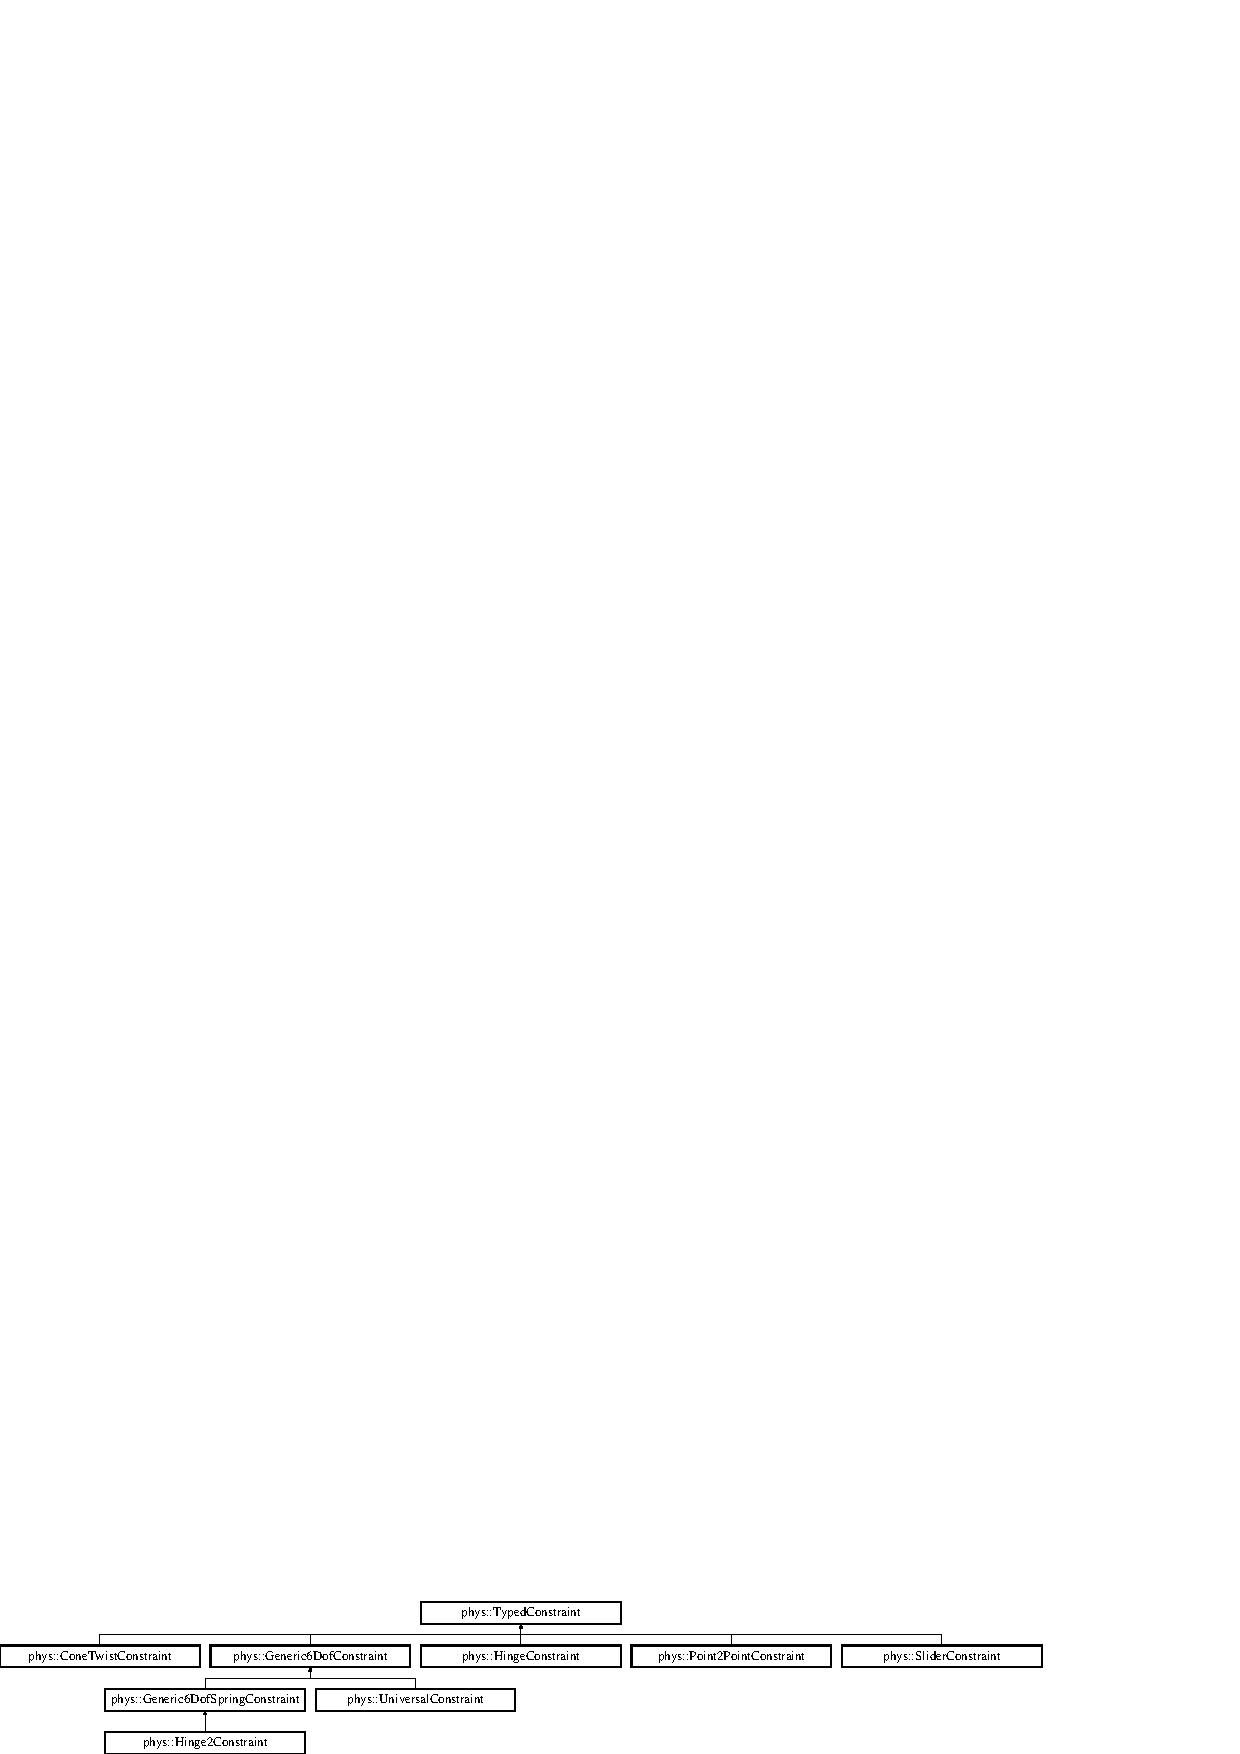
\includegraphics[height=2.045662cm]{d1/d17/classphys_1_1TypedConstraint}
\end{center}
\end{figure}
\subsection*{Public Member Functions}
\begin{DoxyCompactItemize}
\item 
\hyperlink{classphys_1_1TypedConstraint_a499e2f94ca4ee111001efa0dd3862391}{TypedConstraint} ()
\begin{DoxyCompactList}\small\item\em No initialization constructor. \item\end{DoxyCompactList}\item 
virtual \hyperlink{classphys_1_1TypedConstraint_abf1cb6e3cf5c62feac31805162ec2766}{$\sim$TypedConstraint} ()
\begin{DoxyCompactList}\small\item\em Class destructor. \item\end{DoxyCompactList}\item 
\hyperlink{classphys_1_1TypedConstraint_a50ca8631a6c75bbc609c8d4ed61fdcee}{TypedConstraint} (\hyperlink{classphys_1_1ActorRigid}{ActorRigid} $\ast$bodya, \hyperlink{classphys_1_1ActorRigid}{ActorRigid} $\ast$bodyb)
\begin{DoxyCompactList}\small\item\em Two body constructor. \item\end{DoxyCompactList}\item 
\hyperlink{classphys_1_1TypedConstraint_a41ad08bfde377e91f2b37b0af40a9d34}{TypedConstraint} (\hyperlink{classphys_1_1ActorRigid}{ActorRigid} $\ast$bodya)
\begin{DoxyCompactList}\small\item\em One body constructor. \item\end{DoxyCompactList}\item 
\hyperlink{classphys_1_1ActorRigid}{ActorRigid} $\ast$ \hyperlink{classphys_1_1TypedConstraint_aae01815d877566ae4e100bb481ed2f5e}{GetActorA} ()
\begin{DoxyCompactList}\small\item\em Gets the first actor this constraint applies to. \item\end{DoxyCompactList}\item 
\hyperlink{classphys_1_1ActorRigid}{ActorRigid} $\ast$ \hyperlink{classphys_1_1TypedConstraint_a5d988a4d724ed77ca846417d466e9e1a}{GetActorB} ()
\begin{DoxyCompactList}\small\item\em Gets the second actor this constraint applies to. \item\end{DoxyCompactList}\item 
virtual void \hyperlink{classphys_1_1TypedConstraint_a31a20a74094f0cb8e4f82d1f99725415}{SetParam} (int num, \hyperlink{namespacephys_af7eb897198d265b8e868f45240230d5f}{Real} value, int axis=-\/1)=0
\begin{DoxyCompactList}\small\item\em Provides override of constraint parameters. \item\end{DoxyCompactList}\item 
virtual \hyperlink{namespacephys_af7eb897198d265b8e868f45240230d5f}{Real} \hyperlink{classphys_1_1TypedConstraint_ab6140d40e9476c3dc46e2802e8097421}{GetParam} (int num, int axis=-\/1)=0
\begin{DoxyCompactList}\small\item\em Gets value of constraint parameters. \item\end{DoxyCompactList}\end{DoxyCompactItemize}
\subsection*{Protected Attributes}
\begin{DoxyCompactItemize}
\item 
\hypertarget{classphys_1_1TypedConstraint_a5e4251df846e7afbab2e49039530a140}{
btRigidBody $\ast$ \hyperlink{classphys_1_1TypedConstraint_a5e4251df846e7afbab2e49039530a140}{BodyA}}
\label{d1/d17/classphys_1_1TypedConstraint_a5e4251df846e7afbab2e49039530a140}

\begin{DoxyCompactList}\small\item\em First rigid body the constraint applies to. \item\end{DoxyCompactList}\item 
\hypertarget{classphys_1_1TypedConstraint_ab90a86274d18f45628e91a76d28c8278}{
btRigidBody $\ast$ \hyperlink{classphys_1_1TypedConstraint_ab90a86274d18f45628e91a76d28c8278}{BodyB}}
\label{d1/d17/classphys_1_1TypedConstraint_ab90a86274d18f45628e91a76d28c8278}

\begin{DoxyCompactList}\small\item\em Second rigid body the constraint applies to(if applicable). \item\end{DoxyCompactList}\item 
\hypertarget{classphys_1_1TypedConstraint_a0fefb80c80d433bec9942b851b2f5a8a}{
\hyperlink{classphys_1_1ActorRigid}{ActorRigid} $\ast$ \hyperlink{classphys_1_1TypedConstraint_a0fefb80c80d433bec9942b851b2f5a8a}{ActorA}}
\label{d1/d17/classphys_1_1TypedConstraint_a0fefb80c80d433bec9942b851b2f5a8a}

\begin{DoxyCompactList}\small\item\em First Actor the constraint applies to. \item\end{DoxyCompactList}\item 
\hypertarget{classphys_1_1TypedConstraint_a04d2c49698d9a161e92112dd1efc1dcd}{
\hyperlink{classphys_1_1ActorRigid}{ActorRigid} $\ast$ \hyperlink{classphys_1_1TypedConstraint_a04d2c49698d9a161e92112dd1efc1dcd}{ActorB}}
\label{d1/d17/classphys_1_1TypedConstraint_a04d2c49698d9a161e92112dd1efc1dcd}

\begin{DoxyCompactList}\small\item\em Second Actor the constraint applies to. \item\end{DoxyCompactList}\item 
\hypertarget{classphys_1_1TypedConstraint_a31527f4782a0861fd6fd4bb7e201b23f}{
btTypedConstraint $\ast$ \hyperlink{classphys_1_1TypedConstraint_a31527f4782a0861fd6fd4bb7e201b23f}{ConstraintBase}}
\label{d1/d17/classphys_1_1TypedConstraint_a31527f4782a0861fd6fd4bb7e201b23f}

\begin{DoxyCompactList}\small\item\em Bullet constraint that this class encapsulates. \item\end{DoxyCompactList}\end{DoxyCompactItemize}
\subsection*{Friends}
\begin{DoxyCompactItemize}
\item 
\hypertarget{classphys_1_1TypedConstraint_a7b4bcdf992c21ae83363f25df05b1d25}{
class {\bfseries World}}
\label{d1/d17/classphys_1_1TypedConstraint_a7b4bcdf992c21ae83363f25df05b1d25}

\item 
\hypertarget{classphys_1_1TypedConstraint_a139cf05ac01161b7071c8a037c841683}{
class {\bfseries PhysicsManager}}
\label{d1/d17/classphys_1_1TypedConstraint_a139cf05ac01161b7071c8a037c841683}

\end{DoxyCompactItemize}


\subsection{Detailed Description}
This is the base class for all constraints supported. This class provides the basis for all the other constraints. This is also a virtual class and provides no constraint properties of it's own, thus shouldn't/can't be called on manually. 

Definition at line 74 of file constraint.h.



\subsection{Constructor \& Destructor Documentation}
\hypertarget{classphys_1_1TypedConstraint_a499e2f94ca4ee111001efa0dd3862391}{
\index{phys::TypedConstraint@{phys::TypedConstraint}!TypedConstraint@{TypedConstraint}}
\index{TypedConstraint@{TypedConstraint}!phys::TypedConstraint@{phys::TypedConstraint}}
\subsubsection[{TypedConstraint}]{\setlength{\rightskip}{0pt plus 5cm}phys::TypedConstraint::TypedConstraint (
\begin{DoxyParamCaption}
{}
\end{DoxyParamCaption}
)}}
\label{d1/d17/classphys_1_1TypedConstraint_a499e2f94ca4ee111001efa0dd3862391}


No initialization constructor. 

The no initialization class constructor. 

Definition at line 52 of file constraint.cpp.

\hypertarget{classphys_1_1TypedConstraint_abf1cb6e3cf5c62feac31805162ec2766}{
\index{phys::TypedConstraint@{phys::TypedConstraint}!$\sim$TypedConstraint@{$\sim$TypedConstraint}}
\index{$\sim$TypedConstraint@{$\sim$TypedConstraint}!phys::TypedConstraint@{phys::TypedConstraint}}
\subsubsection[{$\sim$TypedConstraint}]{\setlength{\rightskip}{0pt plus 5cm}phys::TypedConstraint::$\sim$TypedConstraint (
\begin{DoxyParamCaption}
{}
\end{DoxyParamCaption}
)\hspace{0.3cm}{\ttfamily  \mbox{[}virtual\mbox{]}}}}
\label{d1/d17/classphys_1_1TypedConstraint_abf1cb6e3cf5c62feac31805162ec2766}


Class destructor. 

The class destructor. 

Definition at line 74 of file constraint.cpp.

\hypertarget{classphys_1_1TypedConstraint_a50ca8631a6c75bbc609c8d4ed61fdcee}{
\index{phys::TypedConstraint@{phys::TypedConstraint}!TypedConstraint@{TypedConstraint}}
\index{TypedConstraint@{TypedConstraint}!phys::TypedConstraint@{phys::TypedConstraint}}
\subsubsection[{TypedConstraint}]{\setlength{\rightskip}{0pt plus 5cm}phys::TypedConstraint::TypedConstraint (
\begin{DoxyParamCaption}
\item[{{\bf ActorRigid} $\ast$}]{ bodya, }
\item[{{\bf ActorRigid} $\ast$}]{ bodyb}
\end{DoxyParamCaption}
)}}
\label{d1/d17/classphys_1_1TypedConstraint_a50ca8631a6c75bbc609c8d4ed61fdcee}


Two body constructor. 

This constructor is used when the applicable constraint is applied to two bodies, as opposed to a point a world space. 
\begin{DoxyParams}{Parameters}
\item[{\em bodya}]First actor to be applied to. \item[{\em bodyb}]Second actor to be applied to. \end{DoxyParams}


Definition at line 56 of file constraint.cpp.

\hypertarget{classphys_1_1TypedConstraint_a41ad08bfde377e91f2b37b0af40a9d34}{
\index{phys::TypedConstraint@{phys::TypedConstraint}!TypedConstraint@{TypedConstraint}}
\index{TypedConstraint@{TypedConstraint}!phys::TypedConstraint@{phys::TypedConstraint}}
\subsubsection[{TypedConstraint}]{\setlength{\rightskip}{0pt plus 5cm}phys::TypedConstraint::TypedConstraint (
\begin{DoxyParamCaption}
\item[{{\bf ActorRigid} $\ast$}]{ bodya}
\end{DoxyParamCaption}
)}}
\label{d1/d17/classphys_1_1TypedConstraint_a41ad08bfde377e91f2b37b0af40a9d34}


One body constructor. 

This constructor is used when the applicable constraint is applied to a body and a point in world space. 
\begin{DoxyParams}{Parameters}
\item[{\em bodya}]The actor to be constraint to a point in world space. \end{DoxyParams}


Definition at line 65 of file constraint.cpp.



\subsection{Member Function Documentation}
\hypertarget{classphys_1_1TypedConstraint_aae01815d877566ae4e100bb481ed2f5e}{
\index{phys::TypedConstraint@{phys::TypedConstraint}!GetActorA@{GetActorA}}
\index{GetActorA@{GetActorA}!phys::TypedConstraint@{phys::TypedConstraint}}
\subsubsection[{GetActorA}]{\setlength{\rightskip}{0pt plus 5cm}{\bf ActorRigid} $\ast$ phys::TypedConstraint::GetActorA (
\begin{DoxyParamCaption}
{}
\end{DoxyParamCaption}
)}}
\label{d1/d17/classphys_1_1TypedConstraint_aae01815d877566ae4e100bb481ed2f5e}


Gets the first actor this constraint applies to. 

\begin{DoxyReturn}{Returns}
Returns a pointer to the first actor this constraint applies to. 
\end{DoxyReturn}


Definition at line 78 of file constraint.cpp.

\hypertarget{classphys_1_1TypedConstraint_a5d988a4d724ed77ca846417d466e9e1a}{
\index{phys::TypedConstraint@{phys::TypedConstraint}!GetActorB@{GetActorB}}
\index{GetActorB@{GetActorB}!phys::TypedConstraint@{phys::TypedConstraint}}
\subsubsection[{GetActorB}]{\setlength{\rightskip}{0pt plus 5cm}{\bf ActorRigid} $\ast$ phys::TypedConstraint::GetActorB (
\begin{DoxyParamCaption}
{}
\end{DoxyParamCaption}
)}}
\label{d1/d17/classphys_1_1TypedConstraint_a5d988a4d724ed77ca846417d466e9e1a}


Gets the second actor this constraint applies to. 

\begin{DoxyReturn}{Returns}
Returns a pointer to the second actor this constraint applies to. 
\end{DoxyReturn}


Definition at line 83 of file constraint.cpp.

\hypertarget{classphys_1_1TypedConstraint_ab6140d40e9476c3dc46e2802e8097421}{
\index{phys::TypedConstraint@{phys::TypedConstraint}!GetParam@{GetParam}}
\index{GetParam@{GetParam}!phys::TypedConstraint@{phys::TypedConstraint}}
\subsubsection[{GetParam}]{\setlength{\rightskip}{0pt plus 5cm}virtual {\bf Real} phys::TypedConstraint::GetParam (
\begin{DoxyParamCaption}
\item[{int}]{ num, }
\item[{int}]{ axis = {\ttfamily -\/1}}
\end{DoxyParamCaption}
)\hspace{0.3cm}{\ttfamily  \mbox{[}pure virtual\mbox{]}}}}
\label{d1/d17/classphys_1_1TypedConstraint_ab6140d40e9476c3dc46e2802e8097421}


Gets value of constraint parameters. 

See \hyperlink{classphys_1_1TypedConstraint_a31a20a74094f0cb8e4f82d1f99725415}{SetParam()} for clarification. Gets information on constraint parameters. 
\begin{DoxyParams}{Parameters}
\item[{\em num}]The parameter to get information for. \item[{\em axis}]Optional axis. \end{DoxyParams}
\begin{DoxyReturn}{Returns}
Returns the value for the requested parameter. 
\end{DoxyReturn}


Implemented in \hyperlink{classphys_1_1ConeTwistConstraint_aab54f6c56622cef4314d3bbff194421e}{phys::ConeTwistConstraint}, \hyperlink{classphys_1_1Generic6DofConstraint_a822152201f9bd6d0a3e1512fa25b3f49}{phys::Generic6DofConstraint}, \hyperlink{classphys_1_1HingeConstraint_a7e8c001ee6291bf457c9860124cacaf8}{phys::HingeConstraint}, \hyperlink{classphys_1_1Point2PointConstraint_a0f58e2b57a463fe6fe44e7b3192fc3b7}{phys::Point2PointConstraint}, and \hyperlink{classphys_1_1SliderConstraint_a181393c2beec42bdebf7d1a17dfe7593}{phys::SliderConstraint}.

\hypertarget{classphys_1_1TypedConstraint_a31a20a74094f0cb8e4f82d1f99725415}{
\index{phys::TypedConstraint@{phys::TypedConstraint}!SetParam@{SetParam}}
\index{SetParam@{SetParam}!phys::TypedConstraint@{phys::TypedConstraint}}
\subsubsection[{SetParam}]{\setlength{\rightskip}{0pt plus 5cm}virtual void phys::TypedConstraint::SetParam (
\begin{DoxyParamCaption}
\item[{int}]{ num, }
\item[{{\bf Real}}]{ value, }
\item[{int}]{ axis = {\ttfamily -\/1}}
\end{DoxyParamCaption}
)\hspace{0.3cm}{\ttfamily  \mbox{[}pure virtual\mbox{]}}}}
\label{d1/d17/classphys_1_1TypedConstraint_a31a20a74094f0cb8e4f82d1f99725415}


Provides override of constraint parameters. 

Parameters such as ERP and CFM can be altered with this function. Optionally provide axis. 
\begin{DoxyParams}{Parameters}
\item[{\em num}]The parameter to override. \item[{\em value}]The new value for the parameter. \item[{\em axis}]Optional axis. \end{DoxyParams}


Implemented in \hyperlink{classphys_1_1ConeTwistConstraint_a555fc33b10a0c156e0ac93b94587098a}{phys::ConeTwistConstraint}, \hyperlink{classphys_1_1Generic6DofConstraint_a644245f0533a2fe1586609fcf1f48171}{phys::Generic6DofConstraint}, \hyperlink{classphys_1_1HingeConstraint_adec79d062d67532e3521eaae6b49f877}{phys::HingeConstraint}, \hyperlink{classphys_1_1Point2PointConstraint_ad6f28464773121658e54e8bde2a14704}{phys::Point2PointConstraint}, and \hyperlink{classphys_1_1SliderConstraint_a1516aeff86674a969411b17a1847d115}{phys::SliderConstraint}.



The documentation for this class was generated from the following files:\begin{DoxyCompactItemize}
\item 
constraint.h\item 
constraint.cpp\end{DoxyCompactItemize}

\hypertarget{classphys_1_1UILayer}{
\section{phys::UILayer Class Reference}
\label{da/d48/classphys_1_1UILayer}\index{phys::UILayer@{phys::UILayer}}
}


This class is the basic container class for UI elements.  




{\ttfamily \#include $<$uilayer.h$>$}

\subsection*{Public Member Functions}
\begin{DoxyCompactItemize}
\item 
\hyperlink{classphys_1_1UILayer_aee4df9be8deb377bc7905c785ddf2819}{UILayer} (const \hyperlink{namespacephys_aa03900411993de7fbfec4789bc1d392e}{String} \&name, Gorilla::Layer $\ast$GLayer, Gorilla::Screen $\ast$GScreen)
\begin{DoxyCompactList}\small\item\em Internal constructor. \item\end{DoxyCompactList}\item 
\hypertarget{classphys_1_1UILayer_ac09b13a0ebae1a2ed99f689c70ada5e5}{
\hyperlink{classphys_1_1UILayer_ac09b13a0ebae1a2ed99f689c70ada5e5}{$\sim$UILayer} ()}
\label{da/d48/classphys_1_1UILayer_ac09b13a0ebae1a2ed99f689c70ada5e5}

\begin{DoxyCompactList}\small\item\em Class destructor. \item\end{DoxyCompactList}\item 
\hyperlink{namespacephys_aa03900411993de7fbfec4789bc1d392e}{String} \& \hyperlink{classphys_1_1UILayer_af69573dd43356fa8cf1672ac405f788e}{GetName} ()
\begin{DoxyCompactList}\small\item\em Gets the name of this layer. \item\end{DoxyCompactList}\item 
void \hyperlink{classphys_1_1UILayer_a466e35a0362e5f8f47c35e646075432c}{SetVisible} (bool Visible)
\begin{DoxyCompactList}\small\item\em Sets the layers' visability. \item\end{DoxyCompactList}\item 
bool \hyperlink{classphys_1_1UILayer_a2d4aaa7627339d7139d7a453ccf55ade}{GetVisible} ()
\begin{DoxyCompactList}\small\item\em Gets the layers' visability. \item\end{DoxyCompactList}\item 
\hypertarget{classphys_1_1UILayer_abb27a523942cd5502cadce7fd6c45870}{
void \hyperlink{classphys_1_1UILayer_abb27a523942cd5502cadce7fd6c45870}{Show} ()}
\label{da/d48/classphys_1_1UILayer_abb27a523942cd5502cadce7fd6c45870}

\begin{DoxyCompactList}\small\item\em Forces the layer to be shown. \item\end{DoxyCompactList}\item 
\hypertarget{classphys_1_1UILayer_a9ebf49907574502a39a5d08450b78af6}{
void \hyperlink{classphys_1_1UILayer_a9ebf49907574502a39a5d08450b78af6}{Hide} ()}
\label{da/d48/classphys_1_1UILayer_a9ebf49907574502a39a5d08450b78af6}

\begin{DoxyCompactList}\small\item\em Forces the layer to hide. \item\end{DoxyCompactList}\item 
\hyperlink{classphys_1_1UI_1_1Button}{UI::Button} $\ast$ \hyperlink{classphys_1_1UILayer_a270b0e2e2d7e48efe0df54f769f930e4}{CreateButton} (\hyperlink{namespacephys_a5ce5049f8b4bf88d6413c47b504ebb31}{ConstString} \&Name, \hyperlink{classphys_1_1Vector2}{Vector2} Position, \hyperlink{classphys_1_1Vector2}{Vector2} Size)
\begin{DoxyCompactList}\small\item\em Creates a button within this layer. \item\end{DoxyCompactList}\item 
\hyperlink{classphys_1_1UI_1_1TextButton}{UI::TextButton} $\ast$ \hyperlink{classphys_1_1UILayer_a734a98ef447b774cae7fd386e0624710}{CreateTextButton} (\hyperlink{namespacephys_a5ce5049f8b4bf88d6413c47b504ebb31}{ConstString} \&Name, \hyperlink{classphys_1_1Vector2}{Vector2} Position, \hyperlink{classphys_1_1Vector2}{Vector2} Size, \hyperlink{namespacephys_a460f6bc24c8dd347b05e0366ae34f34a}{Whole} Glyph, \hyperlink{namespacephys_a5ce5049f8b4bf88d6413c47b504ebb31}{ConstString} Text)
\begin{DoxyCompactList}\small\item\em Creates a text button within this layer. \item\end{DoxyCompactList}\item 
\hyperlink{classphys_1_1UI_1_1Button}{UI::Button} $\ast$ \hyperlink{classphys_1_1UILayer_ace0f4fa9270b252dd593212182d43ebf}{GetButton} (\hyperlink{namespacephys_a5ce5049f8b4bf88d6413c47b504ebb31}{ConstString} \&Name)
\begin{DoxyCompactList}\small\item\em Gets an already created button by name. \item\end{DoxyCompactList}\item 
\hyperlink{classphys_1_1UI_1_1Button}{UI::Button} $\ast$ \hyperlink{classphys_1_1UILayer_a98acc74c401ba1b28c53f1ea8966b950}{GetButton} (\hyperlink{namespacephys_a460f6bc24c8dd347b05e0366ae34f34a}{Whole} Index)
\begin{DoxyCompactList}\small\item\em Gets an already created button by index. \item\end{DoxyCompactList}\item 
\hyperlink{namespacephys_a460f6bc24c8dd347b05e0366ae34f34a}{Whole} \hyperlink{classphys_1_1UILayer_a07ff0fc6febb6704f6cf78aa5b7a6fb9}{GetNumButtons} ()
\begin{DoxyCompactList}\small\item\em Gets the number of buttons created and stored in this class. \item\end{DoxyCompactList}\item 
void \hyperlink{classphys_1_1UILayer_a8bb2f42fed52d5776d16911ffc4435ee}{DestroyButton} (\hyperlink{classphys_1_1UI_1_1Button}{UI::Button} $\ast$ToBeDestroyed)
\begin{DoxyCompactList}\small\item\em Destroys a button. \item\end{DoxyCompactList}\item 
\hyperlink{classphys_1_1UI_1_1Rectangle}{UI::Rectangle} $\ast$ \hyperlink{classphys_1_1UILayer_ac3a40183555b370737d6f6954ea0f8e3}{CreateRectangle} (\hyperlink{classphys_1_1Vector2}{Vector2} Position, \hyperlink{classphys_1_1Vector2}{Vector2} Size)
\begin{DoxyCompactList}\small\item\em Creates a rectangle within this layer. \item\end{DoxyCompactList}\item 
\hyperlink{classphys_1_1UI_1_1Rectangle}{UI::Rectangle} $\ast$ \hyperlink{classphys_1_1UILayer_afb2b94ddabf0cce255dbd82d4e8a9312}{GetRectangle} (\hyperlink{namespacephys_a460f6bc24c8dd347b05e0366ae34f34a}{Whole} Index)
\begin{DoxyCompactList}\small\item\em Gets an already created rectangle by index. \item\end{DoxyCompactList}\item 
\hyperlink{namespacephys_a460f6bc24c8dd347b05e0366ae34f34a}{Whole} \hyperlink{classphys_1_1UILayer_a42ad4ae8ba37db911270a3b1950b9814}{GetNumRectangles} ()
\begin{DoxyCompactList}\small\item\em Gets the number of rectangles created and stored in this class. \item\end{DoxyCompactList}\item 
void \hyperlink{classphys_1_1UILayer_a4342bebb6cd81518268beb658668b438}{DestroyRectangle} (\hyperlink{classphys_1_1UI_1_1Rectangle}{UI::Rectangle} $\ast$ToBeDestroyed)
\begin{DoxyCompactList}\small\item\em Destroys a rectangle. \item\end{DoxyCompactList}\item 
\hyperlink{classphys_1_1UI_1_1Caption}{UI::Caption} $\ast$ \hyperlink{classphys_1_1UILayer_a859fb1ad868dec6c1f92987780781a27}{CreateCaption} (\hyperlink{namespacephys_a5ce5049f8b4bf88d6413c47b504ebb31}{ConstString} \&Name, \hyperlink{classphys_1_1Vector2}{Vector2} Position, \hyperlink{classphys_1_1Vector2}{Vector2} Size, \hyperlink{namespacephys_a460f6bc24c8dd347b05e0366ae34f34a}{Whole} Glyph, \hyperlink{namespacephys_aa03900411993de7fbfec4789bc1d392e}{String} Text)
\begin{DoxyCompactList}\small\item\em Creates a caption within this layer. \item\end{DoxyCompactList}\item 
\hyperlink{classphys_1_1UI_1_1Caption}{UI::Caption} $\ast$ \hyperlink{classphys_1_1UILayer_a2f9a2b50de833f5c57d4410fd1ea6eba}{GetCaption} (\hyperlink{namespacephys_a5ce5049f8b4bf88d6413c47b504ebb31}{ConstString} \&Name)
\begin{DoxyCompactList}\small\item\em Gets an already created caption by name. \item\end{DoxyCompactList}\item 
\hyperlink{classphys_1_1UI_1_1Caption}{UI::Caption} $\ast$ \hyperlink{classphys_1_1UILayer_a0f087439496766594aa3f94a8ef2ec2b}{GetCaption} (\hyperlink{namespacephys_a460f6bc24c8dd347b05e0366ae34f34a}{Whole} Index)
\begin{DoxyCompactList}\small\item\em Gets an already created caption by index. \item\end{DoxyCompactList}\item 
\hyperlink{namespacephys_a460f6bc24c8dd347b05e0366ae34f34a}{Whole} \hyperlink{classphys_1_1UILayer_a76b9f48b8b40c4e933dc1f3cf624ffbc}{GetNumCaptions} ()
\begin{DoxyCompactList}\small\item\em Gets the number of captions created and stored in this class. \item\end{DoxyCompactList}\item 
void \hyperlink{classphys_1_1UILayer_a5c0ac9bd2b2c41178ccde42812e39210}{DestroyCaption} (\hyperlink{classphys_1_1UI_1_1Caption}{UI::Caption} $\ast$ToBeDestroyed)
\begin{DoxyCompactList}\small\item\em Destroys a caption. \item\end{DoxyCompactList}\item 
\hyperlink{classphys_1_1UI_1_1MarkupText}{UI::MarkupText} $\ast$ \hyperlink{classphys_1_1UILayer_ac3f8812430c9b4f04cae996297e59377}{CreateMarkupText} (\hyperlink{namespacephys_a5ce5049f8b4bf88d6413c47b504ebb31}{ConstString} \&Name, \hyperlink{classphys_1_1Vector2}{Vector2} Position, \hyperlink{namespacephys_a460f6bc24c8dd347b05e0366ae34f34a}{Whole} Glyph, \hyperlink{namespacephys_aa03900411993de7fbfec4789bc1d392e}{String} Text)
\begin{DoxyCompactList}\small\item\em Creates a markup text within this layer. \item\end{DoxyCompactList}\item 
\hyperlink{classphys_1_1UI_1_1MarkupText}{UI::MarkupText} $\ast$ \hyperlink{classphys_1_1UILayer_abadb760dd330e6963e27ad725d44ce74}{GetMarkupText} (\hyperlink{namespacephys_a5ce5049f8b4bf88d6413c47b504ebb31}{ConstString} \&Name)
\begin{DoxyCompactList}\small\item\em Gets an already created markup text by name. \item\end{DoxyCompactList}\item 
\hyperlink{classphys_1_1UI_1_1MarkupText}{UI::MarkupText} $\ast$ \hyperlink{classphys_1_1UILayer_a2f40efc62324c5d2d5c1282f2ea6088d}{GetMarkupText} (\hyperlink{namespacephys_a460f6bc24c8dd347b05e0366ae34f34a}{Whole} Index)
\begin{DoxyCompactList}\small\item\em Gets an already created markup text by index. \item\end{DoxyCompactList}\item 
\hyperlink{namespacephys_a460f6bc24c8dd347b05e0366ae34f34a}{Whole} \hyperlink{classphys_1_1UILayer_a80f4761638d701d8767ad1c0f769985a}{GetNumMarkupTexts} ()
\begin{DoxyCompactList}\small\item\em Gets the number of markup texts created and stored in this class. \item\end{DoxyCompactList}\item 
void \hyperlink{classphys_1_1UILayer_a75d488037b5bcc97e88249de10ba1d64}{DestroyMarkupText} (\hyperlink{classphys_1_1UI_1_1MarkupText}{UI::MarkupText} $\ast$ToBeDestroyed)
\begin{DoxyCompactList}\small\item\em Destroys a markup text. \item\end{DoxyCompactList}\item 
\hypertarget{classphys_1_1UILayer_a2b0fb7ef867d4cdbdf5e51a2d25407dc}{
\hyperlink{classphys_1_1UI_1_1LineList}{UI::LineList} $\ast$ \hyperlink{classphys_1_1UILayer_a2b0fb7ef867d4cdbdf5e51a2d25407dc}{CreateLineList} ()}
\label{da/d48/classphys_1_1UILayer_a2b0fb7ef867d4cdbdf5e51a2d25407dc}

\begin{DoxyCompactList}\small\item\em Creates a line list within this layer. \item\end{DoxyCompactList}\item 
\hyperlink{classphys_1_1UI_1_1LineList}{UI::LineList} $\ast$ \hyperlink{classphys_1_1UILayer_abba7c9e3e937db7091254b2683af5ea1}{GetLineList} (\hyperlink{namespacephys_a460f6bc24c8dd347b05e0366ae34f34a}{Whole} Index)
\begin{DoxyCompactList}\small\item\em Gets an already created line list by index. \item\end{DoxyCompactList}\item 
\hyperlink{namespacephys_a460f6bc24c8dd347b05e0366ae34f34a}{Whole} \hyperlink{classphys_1_1UILayer_a746f83b806660debc3104fd90dc57d32}{GetNumLineLists} ()
\begin{DoxyCompactList}\small\item\em Gets the number of line lists created and stored in this class. \item\end{DoxyCompactList}\item 
void \hyperlink{classphys_1_1UILayer_a8a8cbbfbf37c9d54c12de4c235f52ac2}{DestroyLineList} (\hyperlink{classphys_1_1UI_1_1LineList}{UI::LineList} $\ast$ToBeDestroyed)
\begin{DoxyCompactList}\small\item\em Destroys a line list. \item\end{DoxyCompactList}\item 
\hyperlink{classphys_1_1UI_1_1Widget}{UI::Widget} $\ast$ \hyperlink{classphys_1_1UILayer_afcc3fd6ff5d0731aa57f1012deea7214}{GetWidget} (\hyperlink{namespacephys_a5ce5049f8b4bf88d6413c47b504ebb31}{ConstString} \&Name)
\begin{DoxyCompactList}\small\item\em Gets an already created widget by name. \item\end{DoxyCompactList}\item 
\hyperlink{classphys_1_1UI_1_1Widget}{UI::Widget} $\ast$ \hyperlink{classphys_1_1UILayer_ab16bb514422f10dab03dca0a6f269a66}{GetWidget} (\hyperlink{namespacephys_a460f6bc24c8dd347b05e0366ae34f34a}{Whole} Index)
\begin{DoxyCompactList}\small\item\em Gets an already created widget by index. \item\end{DoxyCompactList}\item 
\hyperlink{namespacephys_a460f6bc24c8dd347b05e0366ae34f34a}{Whole} \hyperlink{classphys_1_1UILayer_aa745147022b7f78cdc5bccca57985459}{GetNumWidgets} ()
\begin{DoxyCompactList}\small\item\em Gets the number of widgets created and stored in this class. \item\end{DoxyCompactList}\item 
void \hyperlink{classphys_1_1UILayer_a5c8d3069ecbc38669251532dc5860e5e}{DestroyWidget} (\hyperlink{classphys_1_1UI_1_1Widget}{UI::Widget} $\ast$ToBeDestroyed)
\begin{DoxyCompactList}\small\item\em Destroys a widget. \item\end{DoxyCompactList}\item 
\hyperlink{classphys_1_1UI_1_1Scrollbar}{UI::Scrollbar} $\ast$ \hyperlink{classphys_1_1UILayer_a50643d43ad6e251aafc817e22c2d6a19}{CreateScrollbar} (\hyperlink{namespacephys_a5ce5049f8b4bf88d6413c47b504ebb31}{ConstString} \&Name, \hyperlink{classphys_1_1Vector2}{Vector2} Position, \hyperlink{classphys_1_1Vector2}{Vector2} Size, UI::ScrollbarStyle Style)
\begin{DoxyCompactList}\small\item\em Creates a Scrollbar within this layer. \item\end{DoxyCompactList}\item 
\hyperlink{classphys_1_1UI_1_1CheckBox}{UI::CheckBox} $\ast$ \hyperlink{classphys_1_1UILayer_ad9a60f201b1c0d9d891ea985a5a3c1e3}{CreateCheckBox} (\hyperlink{namespacephys_a5ce5049f8b4bf88d6413c47b504ebb31}{ConstString} \&Name, \hyperlink{classphys_1_1Vector2}{Vector2} Position, \hyperlink{classphys_1_1Vector2}{Vector2} Size, \hyperlink{namespacephys_a460f6bc24c8dd347b05e0366ae34f34a}{Whole} Glyph, \hyperlink{namespacephys_aa03900411993de7fbfec4789bc1d392e}{String} \&LabelText)
\begin{DoxyCompactList}\small\item\em Creates a CheckBox within this layer. \item\end{DoxyCompactList}\item 
\hyperlink{classphys_1_1UI_1_1ButtonListBox}{UI::ButtonListBox} $\ast$ \hyperlink{classphys_1_1UILayer_aa5634ff2ed12c4168dc3c49ac601b933}{CreateButtonListBox} (\hyperlink{namespacephys_a5ce5049f8b4bf88d6413c47b504ebb31}{ConstString} \&Name, \hyperlink{classphys_1_1Vector2}{Vector2} Position, \hyperlink{classphys_1_1Vector2}{Vector2} Size, \hyperlink{namespacephys_af7eb897198d265b8e868f45240230d5f}{Real} ScrollbarWidth, UI::ScrollbarStyle ScrollbarStyle)
\begin{DoxyCompactList}\small\item\em Creates a Button List Box within this layer. \item\end{DoxyCompactList}\item 
\hyperlink{classphys_1_1UI_1_1ListBox}{UI::ListBox} $\ast$ \hyperlink{classphys_1_1UILayer_ac0901ce99a6fa2e3f4c2b8a44239349e}{CreateListBox} (\hyperlink{namespacephys_a5ce5049f8b4bf88d6413c47b504ebb31}{ConstString} \&Name, \hyperlink{classphys_1_1Vector2}{Vector2} Position, \hyperlink{classphys_1_1Vector2}{Vector2} Size, \hyperlink{namespacephys_af7eb897198d265b8e868f45240230d5f}{Real} ScrollbarWidth, UI::ScrollbarStyle ScrollbarStyle)
\begin{DoxyCompactList}\small\item\em Creates a List Box within this layer. \item\end{DoxyCompactList}\item 
\hyperlink{classphys_1_1UI_1_1Window}{UI::Window} $\ast$ \hyperlink{classphys_1_1UILayer_aaf8ca5a901a7300c63311be66309c6d7}{CreateWidgetWindow} (\hyperlink{namespacephys_a5ce5049f8b4bf88d6413c47b504ebb31}{ConstString} \&Name, \hyperlink{classphys_1_1Vector2}{Vector2} Position, \hyperlink{classphys_1_1Vector2}{Vector2} Size)
\begin{DoxyCompactList}\small\item\em Creates a Window within this layer. \item\end{DoxyCompactList}\item 
\hyperlink{classphys_1_1UI_1_1Menu}{UI::Menu} $\ast$ \hyperlink{classphys_1_1UILayer_abd620dfec955b4f2403ccb038a60f88f}{CreateMenu} (\hyperlink{namespacephys_a5ce5049f8b4bf88d6413c47b504ebb31}{ConstString} Name, \hyperlink{classphys_1_1Vector2}{Vector2} Position, \hyperlink{classphys_1_1Vector2}{Vector2} Size)
\begin{DoxyCompactList}\small\item\em Creates a Menu within this layer. \item\end{DoxyCompactList}\item 
\hyperlink{classphys_1_1UI_1_1Button}{UI::Button} $\ast$ \hyperlink{classphys_1_1UILayer_ac28c19dea53d2b89c5c09a2e29ce8c6d}{CheckButtonMouseIsOver} ()
\begin{DoxyCompactList}\small\item\em Gets the button the mouse is over if any. \item\end{DoxyCompactList}\item 
\hyperlink{classphys_1_1UI_1_1Widget}{UI::Widget} $\ast$ \hyperlink{classphys_1_1UILayer_ae121ca4d2ebb6fec7351a5c1eaab3dfc}{CheckWidgetMouseIsOver} ()
\begin{DoxyCompactList}\small\item\em Gets the widget the mouse is over if any. \item\end{DoxyCompactList}\item 
Gorilla::Layer $\ast$ \hyperlink{classphys_1_1UILayer_a0f1d04779794d4401714b0d8fa90cab5}{GetGorillaLayer} ()
\begin{DoxyCompactList}\small\item\em Gets the internal gorilla layer pointer. \item\end{DoxyCompactList}\end{DoxyCompactItemize}
\subsection*{Protected Attributes}
\begin{DoxyCompactItemize}
\item 
\hypertarget{classphys_1_1UILayer_ac1cfdc64e509e8bf94b10844655ebb6c}{
Gorilla::Layer $\ast$ {\bfseries GorillaLayer}}
\label{da/d48/classphys_1_1UILayer_ac1cfdc64e509e8bf94b10844655ebb6c}

\item 
\hypertarget{classphys_1_1UILayer_a3da8314d7bcab7a0261100969d636abf}{
Gorilla::Screen $\ast$ {\bfseries Parent}}
\label{da/d48/classphys_1_1UILayer_a3da8314d7bcab7a0261100969d636abf}

\item 
\hypertarget{classphys_1_1UILayer_aa6c5cb17111c680c1af20d734dd0a3d7}{
\hyperlink{classphys_1_1UIManager}{UIManager} $\ast$ {\bfseries Manager}}
\label{da/d48/classphys_1_1UILayer_aa6c5cb17111c680c1af20d734dd0a3d7}

\item 
\hypertarget{classphys_1_1UILayer_a26df3b08c7bdcb07eeb9f0633c8d2df8}{
\hyperlink{namespacephys_aa03900411993de7fbfec4789bc1d392e}{String} {\bfseries Name}}
\label{da/d48/classphys_1_1UILayer_a26df3b08c7bdcb07eeb9f0633c8d2df8}

\item 
\hypertarget{classphys_1_1UILayer_ae2a7d6dfb30eff9bec40b6a1a208dae3}{
std::vector$<$ \hyperlink{classphys_1_1UI_1_1Button}{UI::Button} $\ast$ $>$ {\bfseries Buttons}}
\label{da/d48/classphys_1_1UILayer_ae2a7d6dfb30eff9bec40b6a1a208dae3}

\item 
\hypertarget{classphys_1_1UILayer_a5b08f8ae240427c00bba64e544f6d8dd}{
std::vector$<$ \hyperlink{classphys_1_1UI_1_1Rectangle}{UI::Rectangle} $\ast$ $>$ {\bfseries Rectangles}}
\label{da/d48/classphys_1_1UILayer_a5b08f8ae240427c00bba64e544f6d8dd}

\item 
\hypertarget{classphys_1_1UILayer_aa895120d4197d7e255bb6db2eaaa84d7}{
std::vector$<$ \hyperlink{classphys_1_1UI_1_1Caption}{UI::Caption} $\ast$ $>$ {\bfseries Captions}}
\label{da/d48/classphys_1_1UILayer_aa895120d4197d7e255bb6db2eaaa84d7}

\item 
\hypertarget{classphys_1_1UILayer_a3b9913fb2f4142d3d52c899b4347b843}{
std::vector$<$ \hyperlink{classphys_1_1UI_1_1MarkupText}{UI::MarkupText} $\ast$ $>$ {\bfseries MarkupTexts}}
\label{da/d48/classphys_1_1UILayer_a3b9913fb2f4142d3d52c899b4347b843}

\item 
\hypertarget{classphys_1_1UILayer_ac71d32f223284d0b94d91cfc526c3b84}{
std::vector$<$ \hyperlink{classphys_1_1UI_1_1LineList}{UI::LineList} $\ast$ $>$ {\bfseries LineLists}}
\label{da/d48/classphys_1_1UILayer_ac71d32f223284d0b94d91cfc526c3b84}

\item 
\hypertarget{classphys_1_1UILayer_a21707b7751f5184986eb3d73de2581b5}{
std::vector$<$ \hyperlink{classphys_1_1UI_1_1Widget}{UI::Widget} $\ast$ $>$ {\bfseries Widgets}}
\label{da/d48/classphys_1_1UILayer_a21707b7751f5184986eb3d73de2581b5}

\end{DoxyCompactItemize}


\subsection{Detailed Description}
This class is the basic container class for UI elements. A layer is a container for widgets and other UI elements that are visable. 

Definition at line 82 of file uilayer.h.



\subsection{Constructor \& Destructor Documentation}
\hypertarget{classphys_1_1UILayer_aee4df9be8deb377bc7905c785ddf2819}{
\index{phys::UILayer@{phys::UILayer}!UILayer@{UILayer}}
\index{UILayer@{UILayer}!phys::UILayer@{phys::UILayer}}
\subsubsection[{UILayer}]{\setlength{\rightskip}{0pt plus 5cm}phys::UILayer::UILayer (
\begin{DoxyParamCaption}
\item[{const {\bf String} \&}]{ name, }
\item[{Gorilla::Layer $\ast$}]{ GLayer, }
\item[{Gorilla::Screen $\ast$}]{ GScreen}
\end{DoxyParamCaption}
)}}
\label{da/d48/classphys_1_1UILayer_aee4df9be8deb377bc7905c785ddf2819}


Internal constructor. 


\begin{DoxyParams}{Parameters}
\item[{\em name}]The name of this layer. \item[{\em GLayer}]The Gorilla Layer this Layer is based on. \item[{\em GScreen}]The gorilla parent screen to this layer. \end{DoxyParams}


Definition at line 64 of file uilayer.cpp.



\subsection{Member Function Documentation}
\hypertarget{classphys_1_1UILayer_ac28c19dea53d2b89c5c09a2e29ce8c6d}{
\index{phys::UILayer@{phys::UILayer}!CheckButtonMouseIsOver@{CheckButtonMouseIsOver}}
\index{CheckButtonMouseIsOver@{CheckButtonMouseIsOver}!phys::UILayer@{phys::UILayer}}
\subsubsection[{CheckButtonMouseIsOver}]{\setlength{\rightskip}{0pt plus 5cm}{\bf UI::Button} $\ast$ phys::UILayer::CheckButtonMouseIsOver (
\begin{DoxyParamCaption}
{}
\end{DoxyParamCaption}
)}}
\label{da/d48/classphys_1_1UILayer_ac28c19dea53d2b89c5c09a2e29ce8c6d}


Gets the button the mouse is over if any. 

This function searches only the buttons contained in this layer. \begin{DoxyReturn}{Returns}
Returns the button the mouse is over, or NULL if there are none. 
\end{DoxyReturn}


Definition at line 447 of file uilayer.cpp.

\hypertarget{classphys_1_1UILayer_ae121ca4d2ebb6fec7351a5c1eaab3dfc}{
\index{phys::UILayer@{phys::UILayer}!CheckWidgetMouseIsOver@{CheckWidgetMouseIsOver}}
\index{CheckWidgetMouseIsOver@{CheckWidgetMouseIsOver}!phys::UILayer@{phys::UILayer}}
\subsubsection[{CheckWidgetMouseIsOver}]{\setlength{\rightskip}{0pt plus 5cm}{\bf UI::Widget} $\ast$ phys::UILayer::CheckWidgetMouseIsOver (
\begin{DoxyParamCaption}
{}
\end{DoxyParamCaption}
)}}
\label{da/d48/classphys_1_1UILayer_ae121ca4d2ebb6fec7351a5c1eaab3dfc}


Gets the widget the mouse is over if any. 

This function searches only the widgets contained in this layer. \begin{DoxyReturn}{Returns}
Returns the widget the mouse is over, or NULL if there are none. 
\end{DoxyReturn}


Definition at line 468 of file uilayer.cpp.

\hypertarget{classphys_1_1UILayer_a270b0e2e2d7e48efe0df54f769f930e4}{
\index{phys::UILayer@{phys::UILayer}!CreateButton@{CreateButton}}
\index{CreateButton@{CreateButton}!phys::UILayer@{phys::UILayer}}
\subsubsection[{CreateButton}]{\setlength{\rightskip}{0pt plus 5cm}{\bf UI::Button} $\ast$ phys::UILayer::CreateButton (
\begin{DoxyParamCaption}
\item[{{\bf ConstString} \&}]{ Name, }
\item[{{\bf Vector2}}]{ Position, }
\item[{{\bf Vector2}}]{ Size}
\end{DoxyParamCaption}
)}}
\label{da/d48/classphys_1_1UILayer_a270b0e2e2d7e48efe0df54f769f930e4}


Creates a button within this layer. 

This constructor expects relative values for position and size(values from 0.0 to 1.0). \begin{DoxyReturn}{Returns}
Returns a pointer to the created button. 
\end{DoxyReturn}

\begin{DoxyParams}{Parameters}
\item[{\em Name}]The name of the button. \item[{\em Position}]The top left position of the button. \item[{\em Size}]The size of the Button. \end{DoxyParams}


Definition at line 138 of file uilayer.cpp.

\hypertarget{classphys_1_1UILayer_aa5634ff2ed12c4168dc3c49ac601b933}{
\index{phys::UILayer@{phys::UILayer}!CreateButtonListBox@{CreateButtonListBox}}
\index{CreateButtonListBox@{CreateButtonListBox}!phys::UILayer@{phys::UILayer}}
\subsubsection[{CreateButtonListBox}]{\setlength{\rightskip}{0pt plus 5cm}{\bf UI::ButtonListBox} $\ast$ phys::UILayer::CreateButtonListBox (
\begin{DoxyParamCaption}
\item[{{\bf ConstString} \&}]{ Name, }
\item[{{\bf Vector2}}]{ Position, }
\item[{{\bf Vector2}}]{ Size, }
\item[{{\bf Real}}]{ ScrollbarWidth, }
\item[{UI::ScrollbarStyle}]{ ScrollbarStyle}
\end{DoxyParamCaption}
)}}
\label{da/d48/classphys_1_1UILayer_aa5634ff2ed12c4168dc3c49ac601b933}


Creates a Button List Box within this layer. 

This constructor expects relative values for position and size(values from 0.0 to 1.0). \begin{DoxyReturn}{Returns}
Returns a pointer to the created Button List Box. 
\end{DoxyReturn}

\begin{DoxyParams}{Parameters}
\item[{\em Name}]The name of the Button List Box. \item[{\em Position}]The top left position of the Button List Box. \item[{\em Size}]The size of the Button List Box. \item[{\em ScrollbarWidth}]The relative width of the scrollbar thats created with this widget. \item[{\em ScrollbarStyle}]The style of scrollbar you want to create, see Scrollbar documentation for more details. \end{DoxyParams}


Definition at line 419 of file uilayer.cpp.

\hypertarget{classphys_1_1UILayer_a859fb1ad868dec6c1f92987780781a27}{
\index{phys::UILayer@{phys::UILayer}!CreateCaption@{CreateCaption}}
\index{CreateCaption@{CreateCaption}!phys::UILayer@{phys::UILayer}}
\subsubsection[{CreateCaption}]{\setlength{\rightskip}{0pt plus 5cm}{\bf UI::Caption} $\ast$ phys::UILayer::CreateCaption (
\begin{DoxyParamCaption}
\item[{{\bf ConstString} \&}]{ Name, }
\item[{{\bf Vector2}}]{ Position, }
\item[{{\bf Vector2}}]{ Size, }
\item[{{\bf Whole}}]{ Glyph, }
\item[{{\bf String}}]{ Text}
\end{DoxyParamCaption}
)}}
\label{da/d48/classphys_1_1UILayer_a859fb1ad868dec6c1f92987780781a27}


Creates a caption within this layer. 

This constructor expects relative values for position and size(values from 0.0 to 1.0). \begin{DoxyReturn}{Returns}
Returns a pointer to the created caption. 
\end{DoxyReturn}

\begin{DoxyParams}{Parameters}
\item[{\em Name}]The name of this caption. \item[{\em Position}]The top left position of the caption. \item[{\em Size}]The size of the Button. \item[{\em Glyph}]One of the glyphs specified in your gorilla file. Must be valid. \item[{\em Text}]Any text you want printed on the caption. \end{DoxyParams}


Definition at line 218 of file uilayer.cpp.

\hypertarget{classphys_1_1UILayer_ad9a60f201b1c0d9d891ea985a5a3c1e3}{
\index{phys::UILayer@{phys::UILayer}!CreateCheckBox@{CreateCheckBox}}
\index{CreateCheckBox@{CreateCheckBox}!phys::UILayer@{phys::UILayer}}
\subsubsection[{CreateCheckBox}]{\setlength{\rightskip}{0pt plus 5cm}{\bf UI::CheckBox} $\ast$ phys::UILayer::CreateCheckBox (
\begin{DoxyParamCaption}
\item[{{\bf ConstString} \&}]{ Name, }
\item[{{\bf Vector2}}]{ Position, }
\item[{{\bf Vector2}}]{ Size, }
\item[{{\bf Whole}}]{ Glyph, }
\item[{{\bf String} \&}]{ LabelText}
\end{DoxyParamCaption}
)}}
\label{da/d48/classphys_1_1UILayer_ad9a60f201b1c0d9d891ea985a5a3c1e3}


Creates a CheckBox within this layer. 

This constructor expects relative values for position and size(values from 0.0 to 1.0). \begin{DoxyReturn}{Returns}
Returns a pointer to the created CheckBox. 
\end{DoxyReturn}

\begin{DoxyParams}{Parameters}
\item[{\em Name}]The name of the CheckBox. \item[{\em Position}]The top left position of the CheckBox. \item[{\em Size}]The size of the CheckBox. \item[{\em Glyph}]The glyphs to use by default for use with the label. Glyphs are defined in your .gorilla file. \item[{\em LabelText}]The text to display with the label. The label uses the Markup Text class, and thus it's light markup text language. You can also pass in a blank string if you don't wish to have a label, you can create a label after construction. \end{DoxyParams}


Definition at line 412 of file uilayer.cpp.

\hypertarget{classphys_1_1UILayer_ac0901ce99a6fa2e3f4c2b8a44239349e}{
\index{phys::UILayer@{phys::UILayer}!CreateListBox@{CreateListBox}}
\index{CreateListBox@{CreateListBox}!phys::UILayer@{phys::UILayer}}
\subsubsection[{CreateListBox}]{\setlength{\rightskip}{0pt plus 5cm}{\bf UI::ListBox} $\ast$ phys::UILayer::CreateListBox (
\begin{DoxyParamCaption}
\item[{{\bf ConstString} \&}]{ Name, }
\item[{{\bf Vector2}}]{ Position, }
\item[{{\bf Vector2}}]{ Size, }
\item[{{\bf Real}}]{ ScrollbarWidth, }
\item[{UI::ScrollbarStyle}]{ ScrollbarStyle}
\end{DoxyParamCaption}
)}}
\label{da/d48/classphys_1_1UILayer_ac0901ce99a6fa2e3f4c2b8a44239349e}


Creates a List Box within this layer. 

This constructor expects relative values for position and size(values from 0.0 to 1.0). \begin{DoxyReturn}{Returns}
Returns a pointer to the created List Box. 
\end{DoxyReturn}

\begin{DoxyParams}{Parameters}
\item[{\em Name}]The name of the List Box. \item[{\em Position}]The top left position of the List Box. \item[{\em Size}]The size of the List Box. \item[{\em ScrollbarWidth}]The relative width of the scrollbar thats created with this widget. \item[{\em ScrollbarStyle}]The style of scrollbar you want to create, see Scrollbar documentation for more details. \end{DoxyParams}


Definition at line 426 of file uilayer.cpp.

\hypertarget{classphys_1_1UILayer_ac3f8812430c9b4f04cae996297e59377}{
\index{phys::UILayer@{phys::UILayer}!CreateMarkupText@{CreateMarkupText}}
\index{CreateMarkupText@{CreateMarkupText}!phys::UILayer@{phys::UILayer}}
\subsubsection[{CreateMarkupText}]{\setlength{\rightskip}{0pt plus 5cm}{\bf UI::MarkupText} $\ast$ phys::UILayer::CreateMarkupText (
\begin{DoxyParamCaption}
\item[{{\bf ConstString} \&}]{ Name, }
\item[{{\bf Vector2}}]{ Position, }
\item[{{\bf Whole}}]{ Glyph, }
\item[{{\bf String}}]{ Text}
\end{DoxyParamCaption}
)}}
\label{da/d48/classphys_1_1UILayer_ac3f8812430c9b4f04cae996297e59377}


Creates a markup text within this layer. 

This constructor expects relative values for position and size(values from 0.0 to 1.0). \begin{DoxyReturn}{Returns}
Returns a pointer to the created markup text. 
\end{DoxyReturn}

\begin{DoxyParams}{Parameters}
\item[{\em Name}]The name of this markup text. \item[{\em Position}]The top left position of the markup text. \item[{\em Glyph}]One of the glyphs specified in your gorilla file. Must be valid. \item[{\em Text}]Any text you want printed on the markup text. \end{DoxyParams}


Definition at line 261 of file uilayer.cpp.

\hypertarget{classphys_1_1UILayer_abd620dfec955b4f2403ccb038a60f88f}{
\index{phys::UILayer@{phys::UILayer}!CreateMenu@{CreateMenu}}
\index{CreateMenu@{CreateMenu}!phys::UILayer@{phys::UILayer}}
\subsubsection[{CreateMenu}]{\setlength{\rightskip}{0pt plus 5cm}{\bf UI::Menu} $\ast$ phys::UILayer::CreateMenu (
\begin{DoxyParamCaption}
\item[{{\bf ConstString}}]{ Name, }
\item[{{\bf Vector2}}]{ Position, }
\item[{{\bf Vector2}}]{ Size}
\end{DoxyParamCaption}
)}}
\label{da/d48/classphys_1_1UILayer_abd620dfec955b4f2403ccb038a60f88f}


Creates a Menu within this layer. 

This constructor expects relative values for position and size(values from 0.0 to 1.0). \begin{DoxyReturn}{Returns}
Returns a pointer to the created Menu. 
\end{DoxyReturn}

\begin{DoxyParams}{Parameters}
\item[{\em Name}]The name of the Menu. \item[{\em Position}]The top left position of the Menu. \item[{\em Size}]The size of the Menu. \end{DoxyParams}


Definition at line 440 of file uilayer.cpp.

\hypertarget{classphys_1_1UILayer_ac3a40183555b370737d6f6954ea0f8e3}{
\index{phys::UILayer@{phys::UILayer}!CreateRectangle@{CreateRectangle}}
\index{CreateRectangle@{CreateRectangle}!phys::UILayer@{phys::UILayer}}
\subsubsection[{CreateRectangle}]{\setlength{\rightskip}{0pt plus 5cm}{\bf UI::Rectangle} $\ast$ phys::UILayer::CreateRectangle (
\begin{DoxyParamCaption}
\item[{{\bf Vector2}}]{ Position, }
\item[{{\bf Vector2}}]{ Size}
\end{DoxyParamCaption}
)}}
\label{da/d48/classphys_1_1UILayer_ac3a40183555b370737d6f6954ea0f8e3}


Creates a rectangle within this layer. 

This constructor expects relative values for position and size(values from 0.0 to 1.0). \par
 Rectangles are innately put behind all captions, so z-\/order is not necessary. 
\begin{DoxyParams}{Parameters}
\item[{\em Position}]The top left position of the button. \item[{\em Size}]The size of the Button. \end{DoxyParams}


Definition at line 188 of file uilayer.cpp.

\hypertarget{classphys_1_1UILayer_a50643d43ad6e251aafc817e22c2d6a19}{
\index{phys::UILayer@{phys::UILayer}!CreateScrollbar@{CreateScrollbar}}
\index{CreateScrollbar@{CreateScrollbar}!phys::UILayer@{phys::UILayer}}
\subsubsection[{CreateScrollbar}]{\setlength{\rightskip}{0pt plus 5cm}{\bf UI::Scrollbar} $\ast$ phys::UILayer::CreateScrollbar (
\begin{DoxyParamCaption}
\item[{{\bf ConstString} \&}]{ Name, }
\item[{{\bf Vector2}}]{ Position, }
\item[{{\bf Vector2}}]{ Size, }
\item[{UI::ScrollbarStyle}]{ Style}
\end{DoxyParamCaption}
)}}
\label{da/d48/classphys_1_1UILayer_a50643d43ad6e251aafc817e22c2d6a19}


Creates a Scrollbar within this layer. 

This constructor expects relative values for position and size(values from 0.0 to 1.0). \begin{DoxyReturn}{Returns}
Returns a pointer to the created Scrollbar. 
\end{DoxyReturn}

\begin{DoxyParams}{Parameters}
\item[{\em Name}]The name of the Scrollbar. \item[{\em Position}]The top left position of the Scrollbar. \item[{\em Size}]The size of the Scrollbar. \item[{\em Style}]The style of scrollbar you want to create, see Scrollbar documentation for more details. \end{DoxyParams}


Definition at line 405 of file uilayer.cpp.

\hypertarget{classphys_1_1UILayer_a734a98ef447b774cae7fd386e0624710}{
\index{phys::UILayer@{phys::UILayer}!CreateTextButton@{CreateTextButton}}
\index{CreateTextButton@{CreateTextButton}!phys::UILayer@{phys::UILayer}}
\subsubsection[{CreateTextButton}]{\setlength{\rightskip}{0pt plus 5cm}{\bf UI::TextButton} $\ast$ phys::UILayer::CreateTextButton (
\begin{DoxyParamCaption}
\item[{{\bf ConstString} \&}]{ Name, }
\item[{{\bf Vector2}}]{ Position, }
\item[{{\bf Vector2}}]{ Size, }
\item[{{\bf Whole}}]{ Glyph, }
\item[{{\bf ConstString}}]{ Text}
\end{DoxyParamCaption}
)}}
\label{da/d48/classphys_1_1UILayer_a734a98ef447b774cae7fd386e0624710}


Creates a text button within this layer. 

This constructor expects relative values for position and size(values from 0.0 to 1.0). \begin{DoxyReturn}{Returns}
Returns a pointer to the created button. 
\end{DoxyReturn}

\begin{DoxyParams}{Parameters}
\item[{\em Name}]The name of the button. \item[{\em Position}]The top left position of the button. \item[{\em Size}]The size of the Button. \item[{\em Glyph}]One of the glyphs specified in your gorilla file. Must be valid. \item[{\em Text}]Any text you want printed on the button. \end{DoxyParams}


Definition at line 145 of file uilayer.cpp.

\hypertarget{classphys_1_1UILayer_aaf8ca5a901a7300c63311be66309c6d7}{
\index{phys::UILayer@{phys::UILayer}!CreateWidgetWindow@{CreateWidgetWindow}}
\index{CreateWidgetWindow@{CreateWidgetWindow}!phys::UILayer@{phys::UILayer}}
\subsubsection[{CreateWidgetWindow}]{\setlength{\rightskip}{0pt plus 5cm}{\bf UI::Window} $\ast$ phys::UILayer::CreateWidgetWindow (
\begin{DoxyParamCaption}
\item[{{\bf ConstString} \&}]{ Name, }
\item[{{\bf Vector2}}]{ Position, }
\item[{{\bf Vector2}}]{ Size}
\end{DoxyParamCaption}
)}}
\label{da/d48/classphys_1_1UILayer_aaf8ca5a901a7300c63311be66309c6d7}


Creates a Window within this layer. 

This constructor expects relative values for position and size(values from 0.0 to 1.0). \begin{DoxyReturn}{Returns}
Returns a pointer to the created Window. 
\end{DoxyReturn}

\begin{DoxyParams}{Parameters}
\item[{\em Name}]The name of the Window. \item[{\em Position}]The top left position of the Window. \item[{\em Size}]The size of the Window. \end{DoxyParams}


Definition at line 433 of file uilayer.cpp.

\hypertarget{classphys_1_1UILayer_a8bb2f42fed52d5776d16911ffc4435ee}{
\index{phys::UILayer@{phys::UILayer}!DestroyButton@{DestroyButton}}
\index{DestroyButton@{DestroyButton}!phys::UILayer@{phys::UILayer}}
\subsubsection[{DestroyButton}]{\setlength{\rightskip}{0pt plus 5cm}void phys::UILayer::DestroyButton (
\begin{DoxyParamCaption}
\item[{{\bf UI::Button} $\ast$}]{ ToBeDestroyed}
\end{DoxyParamCaption}
)}}
\label{da/d48/classphys_1_1UILayer_a8bb2f42fed52d5776d16911ffc4435ee}


Destroys a button. 


\begin{DoxyParams}{Parameters}
\item[{\em ToBeDestroyed}]Pointer to the button you want destroyed. \end{DoxyParams}


Definition at line 175 of file uilayer.cpp.

\hypertarget{classphys_1_1UILayer_a5c0ac9bd2b2c41178ccde42812e39210}{
\index{phys::UILayer@{phys::UILayer}!DestroyCaption@{DestroyCaption}}
\index{DestroyCaption@{DestroyCaption}!phys::UILayer@{phys::UILayer}}
\subsubsection[{DestroyCaption}]{\setlength{\rightskip}{0pt plus 5cm}void phys::UILayer::DestroyCaption (
\begin{DoxyParamCaption}
\item[{{\bf UI::Caption} $\ast$}]{ ToBeDestroyed}
\end{DoxyParamCaption}
)}}
\label{da/d48/classphys_1_1UILayer_a5c0ac9bd2b2c41178ccde42812e39210}


Destroys a caption. 


\begin{DoxyParams}{Parameters}
\item[{\em ToBeDestroyed}]Pointer to the caption you want destroyed. \end{DoxyParams}


Definition at line 248 of file uilayer.cpp.

\hypertarget{classphys_1_1UILayer_a8a8cbbfbf37c9d54c12de4c235f52ac2}{
\index{phys::UILayer@{phys::UILayer}!DestroyLineList@{DestroyLineList}}
\index{DestroyLineList@{DestroyLineList}!phys::UILayer@{phys::UILayer}}
\subsubsection[{DestroyLineList}]{\setlength{\rightskip}{0pt plus 5cm}void phys::UILayer::DestroyLineList (
\begin{DoxyParamCaption}
\item[{{\bf UI::LineList} $\ast$}]{ ToBeDestroyed}
\end{DoxyParamCaption}
)}}
\label{da/d48/classphys_1_1UILayer_a8a8cbbfbf37c9d54c12de4c235f52ac2}


Destroys a line list. 


\begin{DoxyParams}{Parameters}
\item[{\em ToBeDestroyed}]Pointer to the line list you want destroyed. \end{DoxyParams}


Definition at line 321 of file uilayer.cpp.

\hypertarget{classphys_1_1UILayer_a75d488037b5bcc97e88249de10ba1d64}{
\index{phys::UILayer@{phys::UILayer}!DestroyMarkupText@{DestroyMarkupText}}
\index{DestroyMarkupText@{DestroyMarkupText}!phys::UILayer@{phys::UILayer}}
\subsubsection[{DestroyMarkupText}]{\setlength{\rightskip}{0pt plus 5cm}void phys::UILayer::DestroyMarkupText (
\begin{DoxyParamCaption}
\item[{{\bf UI::MarkupText} $\ast$}]{ ToBeDestroyed}
\end{DoxyParamCaption}
)}}
\label{da/d48/classphys_1_1UILayer_a75d488037b5bcc97e88249de10ba1d64}


Destroys a markup text. 


\begin{DoxyParams}{Parameters}
\item[{\em ToBeDestroyed}]Pointer to the markup text you want destroyed. \end{DoxyParams}


Definition at line 291 of file uilayer.cpp.

\hypertarget{classphys_1_1UILayer_a4342bebb6cd81518268beb658668b438}{
\index{phys::UILayer@{phys::UILayer}!DestroyRectangle@{DestroyRectangle}}
\index{DestroyRectangle@{DestroyRectangle}!phys::UILayer@{phys::UILayer}}
\subsubsection[{DestroyRectangle}]{\setlength{\rightskip}{0pt plus 5cm}void phys::UILayer::DestroyRectangle (
\begin{DoxyParamCaption}
\item[{{\bf UI::Rectangle} $\ast$}]{ ToBeDestroyed}
\end{DoxyParamCaption}
)}}
\label{da/d48/classphys_1_1UILayer_a4342bebb6cd81518268beb658668b438}


Destroys a rectangle. 


\begin{DoxyParams}{Parameters}
\item[{\em ToBeDestroyed}]Pointer to the rectangle you want destroyed. \end{DoxyParams}


Definition at line 205 of file uilayer.cpp.

\hypertarget{classphys_1_1UILayer_a5c8d3069ecbc38669251532dc5860e5e}{
\index{phys::UILayer@{phys::UILayer}!DestroyWidget@{DestroyWidget}}
\index{DestroyWidget@{DestroyWidget}!phys::UILayer@{phys::UILayer}}
\subsubsection[{DestroyWidget}]{\setlength{\rightskip}{0pt plus 5cm}void phys::UILayer::DestroyWidget (
\begin{DoxyParamCaption}
\item[{{\bf UI::Widget} $\ast$}]{ ToBeDestroyed}
\end{DoxyParamCaption}
)}}
\label{da/d48/classphys_1_1UILayer_a5c8d3069ecbc38669251532dc5860e5e}


Destroys a widget. 


\begin{DoxyParams}{Parameters}
\item[{\em ToBeDestroyed}]Pointer to the widget you want destroyed. \end{DoxyParams}


Definition at line 357 of file uilayer.cpp.

\hypertarget{classphys_1_1UILayer_a98acc74c401ba1b28c53f1ea8966b950}{
\index{phys::UILayer@{phys::UILayer}!GetButton@{GetButton}}
\index{GetButton@{GetButton}!phys::UILayer@{phys::UILayer}}
\subsubsection[{GetButton}]{\setlength{\rightskip}{0pt plus 5cm}{\bf UI::Button} $\ast$ phys::UILayer::GetButton (
\begin{DoxyParamCaption}
\item[{{\bf Whole}}]{ Index}
\end{DoxyParamCaption}
)}}
\label{da/d48/classphys_1_1UILayer_a98acc74c401ba1b28c53f1ea8966b950}


Gets an already created button by index. 

\begin{DoxyReturn}{Returns}
Returns a pointer to the button at the specified index. 
\end{DoxyReturn}


Definition at line 165 of file uilayer.cpp.

\hypertarget{classphys_1_1UILayer_ace0f4fa9270b252dd593212182d43ebf}{
\index{phys::UILayer@{phys::UILayer}!GetButton@{GetButton}}
\index{GetButton@{GetButton}!phys::UILayer@{phys::UILayer}}
\subsubsection[{GetButton}]{\setlength{\rightskip}{0pt plus 5cm}{\bf UI::Button} $\ast$ phys::UILayer::GetButton (
\begin{DoxyParamCaption}
\item[{{\bf ConstString} \&}]{ Name}
\end{DoxyParamCaption}
)}}
\label{da/d48/classphys_1_1UILayer_ace0f4fa9270b252dd593212182d43ebf}


Gets an already created button by name. 

\begin{DoxyReturn}{Returns}
Returns a pointer to the button of the specified name. 
\end{DoxyReturn}


Definition at line 152 of file uilayer.cpp.

\hypertarget{classphys_1_1UILayer_a2f9a2b50de833f5c57d4410fd1ea6eba}{
\index{phys::UILayer@{phys::UILayer}!GetCaption@{GetCaption}}
\index{GetCaption@{GetCaption}!phys::UILayer@{phys::UILayer}}
\subsubsection[{GetCaption}]{\setlength{\rightskip}{0pt plus 5cm}{\bf UI::Caption} $\ast$ phys::UILayer::GetCaption (
\begin{DoxyParamCaption}
\item[{{\bf ConstString} \&}]{ Name}
\end{DoxyParamCaption}
)}}
\label{da/d48/classphys_1_1UILayer_a2f9a2b50de833f5c57d4410fd1ea6eba}


Gets an already created caption by name. 

\begin{DoxyReturn}{Returns}
Returns a pointer to the caption of the specified name. 
\end{DoxyReturn}


Definition at line 225 of file uilayer.cpp.

\hypertarget{classphys_1_1UILayer_a0f087439496766594aa3f94a8ef2ec2b}{
\index{phys::UILayer@{phys::UILayer}!GetCaption@{GetCaption}}
\index{GetCaption@{GetCaption}!phys::UILayer@{phys::UILayer}}
\subsubsection[{GetCaption}]{\setlength{\rightskip}{0pt plus 5cm}{\bf UI::Caption} $\ast$ phys::UILayer::GetCaption (
\begin{DoxyParamCaption}
\item[{{\bf Whole}}]{ Index}
\end{DoxyParamCaption}
)}}
\label{da/d48/classphys_1_1UILayer_a0f087439496766594aa3f94a8ef2ec2b}


Gets an already created caption by index. 

\begin{DoxyReturn}{Returns}
Returns a pointer to the caption at the specified index. 
\end{DoxyReturn}


Definition at line 238 of file uilayer.cpp.

\hypertarget{classphys_1_1UILayer_a0f1d04779794d4401714b0d8fa90cab5}{
\index{phys::UILayer@{phys::UILayer}!GetGorillaLayer@{GetGorillaLayer}}
\index{GetGorillaLayer@{GetGorillaLayer}!phys::UILayer@{phys::UILayer}}
\subsubsection[{GetGorillaLayer}]{\setlength{\rightskip}{0pt plus 5cm}Gorilla::Layer $\ast$ phys::UILayer::GetGorillaLayer (
\begin{DoxyParamCaption}
{}
\end{DoxyParamCaption}
)}}
\label{da/d48/classphys_1_1UILayer_a0f1d04779794d4401714b0d8fa90cab5}


Gets the internal gorilla layer pointer. 

\begin{DoxyInternal}{For internal use only.}
\end{DoxyInternal}


Definition at line 487 of file uilayer.cpp.

\hypertarget{classphys_1_1UILayer_abba7c9e3e937db7091254b2683af5ea1}{
\index{phys::UILayer@{phys::UILayer}!GetLineList@{GetLineList}}
\index{GetLineList@{GetLineList}!phys::UILayer@{phys::UILayer}}
\subsubsection[{GetLineList}]{\setlength{\rightskip}{0pt plus 5cm}{\bf UI::LineList} $\ast$ phys::UILayer::GetLineList (
\begin{DoxyParamCaption}
\item[{{\bf Whole}}]{ Index}
\end{DoxyParamCaption}
)}}
\label{da/d48/classphys_1_1UILayer_abba7c9e3e937db7091254b2683af5ea1}


Gets an already created line list by index. 

\begin{DoxyReturn}{Returns}
Returns a pointer to the line list at the specified index. 
\end{DoxyReturn}


Definition at line 311 of file uilayer.cpp.

\hypertarget{classphys_1_1UILayer_a2f40efc62324c5d2d5c1282f2ea6088d}{
\index{phys::UILayer@{phys::UILayer}!GetMarkupText@{GetMarkupText}}
\index{GetMarkupText@{GetMarkupText}!phys::UILayer@{phys::UILayer}}
\subsubsection[{GetMarkupText}]{\setlength{\rightskip}{0pt plus 5cm}{\bf UI::MarkupText} $\ast$ phys::UILayer::GetMarkupText (
\begin{DoxyParamCaption}
\item[{{\bf Whole}}]{ Index}
\end{DoxyParamCaption}
)}}
\label{da/d48/classphys_1_1UILayer_a2f40efc62324c5d2d5c1282f2ea6088d}


Gets an already created markup text by index. 

\begin{DoxyReturn}{Returns}
Returns a pointer to the markup text at the specified index. 
\end{DoxyReturn}


Definition at line 281 of file uilayer.cpp.

\hypertarget{classphys_1_1UILayer_abadb760dd330e6963e27ad725d44ce74}{
\index{phys::UILayer@{phys::UILayer}!GetMarkupText@{GetMarkupText}}
\index{GetMarkupText@{GetMarkupText}!phys::UILayer@{phys::UILayer}}
\subsubsection[{GetMarkupText}]{\setlength{\rightskip}{0pt plus 5cm}{\bf UI::MarkupText} $\ast$ phys::UILayer::GetMarkupText (
\begin{DoxyParamCaption}
\item[{{\bf ConstString} \&}]{ Name}
\end{DoxyParamCaption}
)}}
\label{da/d48/classphys_1_1UILayer_abadb760dd330e6963e27ad725d44ce74}


Gets an already created markup text by name. 

\begin{DoxyReturn}{Returns}
Returns a pointer to the markup text of the specified name. 
\end{DoxyReturn}


Definition at line 268 of file uilayer.cpp.

\hypertarget{classphys_1_1UILayer_af69573dd43356fa8cf1672ac405f788e}{
\index{phys::UILayer@{phys::UILayer}!GetName@{GetName}}
\index{GetName@{GetName}!phys::UILayer@{phys::UILayer}}
\subsubsection[{GetName}]{\setlength{\rightskip}{0pt plus 5cm}{\bf String} \& phys::UILayer::GetName (
\begin{DoxyParamCaption}
{}
\end{DoxyParamCaption}
)}}
\label{da/d48/classphys_1_1UILayer_af69573dd43356fa8cf1672ac405f788e}


Gets the name of this layer. 

\begin{DoxyReturn}{Returns}
Returns a string containing the name of this layer. 
\end{DoxyReturn}


Definition at line 113 of file uilayer.cpp.

\hypertarget{classphys_1_1UILayer_a07ff0fc6febb6704f6cf78aa5b7a6fb9}{
\index{phys::UILayer@{phys::UILayer}!GetNumButtons@{GetNumButtons}}
\index{GetNumButtons@{GetNumButtons}!phys::UILayer@{phys::UILayer}}
\subsubsection[{GetNumButtons}]{\setlength{\rightskip}{0pt plus 5cm}{\bf Whole} phys::UILayer::GetNumButtons (
\begin{DoxyParamCaption}
{}
\end{DoxyParamCaption}
)}}
\label{da/d48/classphys_1_1UILayer_a07ff0fc6febb6704f6cf78aa5b7a6fb9}


Gets the number of buttons created and stored in this class. 

\begin{DoxyReturn}{Returns}
Returns the number of buttons this class is storing. 
\end{DoxyReturn}


Definition at line 170 of file uilayer.cpp.

\hypertarget{classphys_1_1UILayer_a76b9f48b8b40c4e933dc1f3cf624ffbc}{
\index{phys::UILayer@{phys::UILayer}!GetNumCaptions@{GetNumCaptions}}
\index{GetNumCaptions@{GetNumCaptions}!phys::UILayer@{phys::UILayer}}
\subsubsection[{GetNumCaptions}]{\setlength{\rightskip}{0pt plus 5cm}{\bf Whole} phys::UILayer::GetNumCaptions (
\begin{DoxyParamCaption}
{}
\end{DoxyParamCaption}
)}}
\label{da/d48/classphys_1_1UILayer_a76b9f48b8b40c4e933dc1f3cf624ffbc}


Gets the number of captions created and stored in this class. 

\begin{DoxyReturn}{Returns}
Returns the number of captions this class is storing. 
\end{DoxyReturn}


Definition at line 243 of file uilayer.cpp.

\hypertarget{classphys_1_1UILayer_a746f83b806660debc3104fd90dc57d32}{
\index{phys::UILayer@{phys::UILayer}!GetNumLineLists@{GetNumLineLists}}
\index{GetNumLineLists@{GetNumLineLists}!phys::UILayer@{phys::UILayer}}
\subsubsection[{GetNumLineLists}]{\setlength{\rightskip}{0pt plus 5cm}{\bf Whole} phys::UILayer::GetNumLineLists (
\begin{DoxyParamCaption}
{}
\end{DoxyParamCaption}
)}}
\label{da/d48/classphys_1_1UILayer_a746f83b806660debc3104fd90dc57d32}


Gets the number of line lists created and stored in this class. 

\begin{DoxyReturn}{Returns}
Returns the number of line lists this class is storing. 
\end{DoxyReturn}


Definition at line 316 of file uilayer.cpp.

\hypertarget{classphys_1_1UILayer_a80f4761638d701d8767ad1c0f769985a}{
\index{phys::UILayer@{phys::UILayer}!GetNumMarkupTexts@{GetNumMarkupTexts}}
\index{GetNumMarkupTexts@{GetNumMarkupTexts}!phys::UILayer@{phys::UILayer}}
\subsubsection[{GetNumMarkupTexts}]{\setlength{\rightskip}{0pt plus 5cm}{\bf Whole} phys::UILayer::GetNumMarkupTexts (
\begin{DoxyParamCaption}
{}
\end{DoxyParamCaption}
)}}
\label{da/d48/classphys_1_1UILayer_a80f4761638d701d8767ad1c0f769985a}


Gets the number of markup texts created and stored in this class. 

\begin{DoxyReturn}{Returns}
Returns the number of markup texts this class is storing. 
\end{DoxyReturn}


Definition at line 286 of file uilayer.cpp.

\hypertarget{classphys_1_1UILayer_a42ad4ae8ba37db911270a3b1950b9814}{
\index{phys::UILayer@{phys::UILayer}!GetNumRectangles@{GetNumRectangles}}
\index{GetNumRectangles@{GetNumRectangles}!phys::UILayer@{phys::UILayer}}
\subsubsection[{GetNumRectangles}]{\setlength{\rightskip}{0pt plus 5cm}{\bf Whole} phys::UILayer::GetNumRectangles (
\begin{DoxyParamCaption}
{}
\end{DoxyParamCaption}
)}}
\label{da/d48/classphys_1_1UILayer_a42ad4ae8ba37db911270a3b1950b9814}


Gets the number of rectangles created and stored in this class. 

\begin{DoxyReturn}{Returns}
Returns the number of rectangles this class is storing. 
\end{DoxyReturn}


Definition at line 200 of file uilayer.cpp.

\hypertarget{classphys_1_1UILayer_aa745147022b7f78cdc5bccca57985459}{
\index{phys::UILayer@{phys::UILayer}!GetNumWidgets@{GetNumWidgets}}
\index{GetNumWidgets@{GetNumWidgets}!phys::UILayer@{phys::UILayer}}
\subsubsection[{GetNumWidgets}]{\setlength{\rightskip}{0pt plus 5cm}{\bf Whole} phys::UILayer::GetNumWidgets (
\begin{DoxyParamCaption}
{}
\end{DoxyParamCaption}
)}}
\label{da/d48/classphys_1_1UILayer_aa745147022b7f78cdc5bccca57985459}


Gets the number of widgets created and stored in this class. 

\begin{DoxyReturn}{Returns}
Returns the number of widgets this class is storing. 
\end{DoxyReturn}


Definition at line 352 of file uilayer.cpp.

\hypertarget{classphys_1_1UILayer_afb2b94ddabf0cce255dbd82d4e8a9312}{
\index{phys::UILayer@{phys::UILayer}!GetRectangle@{GetRectangle}}
\index{GetRectangle@{GetRectangle}!phys::UILayer@{phys::UILayer}}
\subsubsection[{GetRectangle}]{\setlength{\rightskip}{0pt plus 5cm}{\bf UI::Rectangle} $\ast$ phys::UILayer::GetRectangle (
\begin{DoxyParamCaption}
\item[{{\bf Whole}}]{ Index}
\end{DoxyParamCaption}
)}}
\label{da/d48/classphys_1_1UILayer_afb2b94ddabf0cce255dbd82d4e8a9312}


Gets an already created rectangle by index. 

\begin{DoxyReturn}{Returns}
Returns a pointer to the rectangle at the specified index. 
\end{DoxyReturn}


Definition at line 195 of file uilayer.cpp.

\hypertarget{classphys_1_1UILayer_a2d4aaa7627339d7139d7a453ccf55ade}{
\index{phys::UILayer@{phys::UILayer}!GetVisible@{GetVisible}}
\index{GetVisible@{GetVisible}!phys::UILayer@{phys::UILayer}}
\subsubsection[{GetVisible}]{\setlength{\rightskip}{0pt plus 5cm}bool phys::UILayer::GetVisible (
\begin{DoxyParamCaption}
{}
\end{DoxyParamCaption}
)}}
\label{da/d48/classphys_1_1UILayer_a2d4aaa7627339d7139d7a453ccf55ade}


Gets the layers' visability. 

\begin{DoxyReturn}{Returns}
Returns a bool representing the visability of the layer. 
\end{DoxyReturn}


Definition at line 123 of file uilayer.cpp.

\hypertarget{classphys_1_1UILayer_afcc3fd6ff5d0731aa57f1012deea7214}{
\index{phys::UILayer@{phys::UILayer}!GetWidget@{GetWidget}}
\index{GetWidget@{GetWidget}!phys::UILayer@{phys::UILayer}}
\subsubsection[{GetWidget}]{\setlength{\rightskip}{0pt plus 5cm}{\bf UI::Widget} $\ast$ phys::UILayer::GetWidget (
\begin{DoxyParamCaption}
\item[{{\bf ConstString} \&}]{ Name}
\end{DoxyParamCaption}
)}}
\label{da/d48/classphys_1_1UILayer_afcc3fd6ff5d0731aa57f1012deea7214}


Gets an already created widget by name. 

\begin{DoxyReturn}{Returns}
Returns a pointer to the widget of the specified name. 
\end{DoxyReturn}


Definition at line 334 of file uilayer.cpp.

\hypertarget{classphys_1_1UILayer_ab16bb514422f10dab03dca0a6f269a66}{
\index{phys::UILayer@{phys::UILayer}!GetWidget@{GetWidget}}
\index{GetWidget@{GetWidget}!phys::UILayer@{phys::UILayer}}
\subsubsection[{GetWidget}]{\setlength{\rightskip}{0pt plus 5cm}{\bf UI::Widget} $\ast$ phys::UILayer::GetWidget (
\begin{DoxyParamCaption}
\item[{{\bf Whole}}]{ Index}
\end{DoxyParamCaption}
)}}
\label{da/d48/classphys_1_1UILayer_ab16bb514422f10dab03dca0a6f269a66}


Gets an already created widget by index. 

\begin{DoxyReturn}{Returns}
Returns a pointer to the widget at the specified index. 
\end{DoxyReturn}


Definition at line 347 of file uilayer.cpp.

\hypertarget{classphys_1_1UILayer_a466e35a0362e5f8f47c35e646075432c}{
\index{phys::UILayer@{phys::UILayer}!SetVisible@{SetVisible}}
\index{SetVisible@{SetVisible}!phys::UILayer@{phys::UILayer}}
\subsubsection[{SetVisible}]{\setlength{\rightskip}{0pt plus 5cm}void phys::UILayer::SetVisible (
\begin{DoxyParamCaption}
\item[{bool}]{ Visible}
\end{DoxyParamCaption}
)}}
\label{da/d48/classphys_1_1UILayer_a466e35a0362e5f8f47c35e646075432c}


Sets the layers' visability. 


\begin{DoxyParams}{Parameters}
\item[{\em Visable}]A bool representing the visability of the layer. \end{DoxyParams}


Definition at line 118 of file uilayer.cpp.



The documentation for this class was generated from the following files:\begin{DoxyCompactItemize}
\item 
uilayer.h\item 
uilayer.cpp\end{DoxyCompactItemize}

\hypertarget{classphys_1_1UIManager}{
\section{phys::UIManager Class Reference}
\label{d5/dc5/classphys_1_1UIManager}\index{phys::UIManager@{phys::UIManager}}
}


This class is responsible for any and all user interactions with the User interface/HUD.  




{\ttfamily \#include $<$uimanager.h$>$}

Inheritance diagram for phys::UIManager:\begin{figure}[H]
\begin{center}
\leavevmode
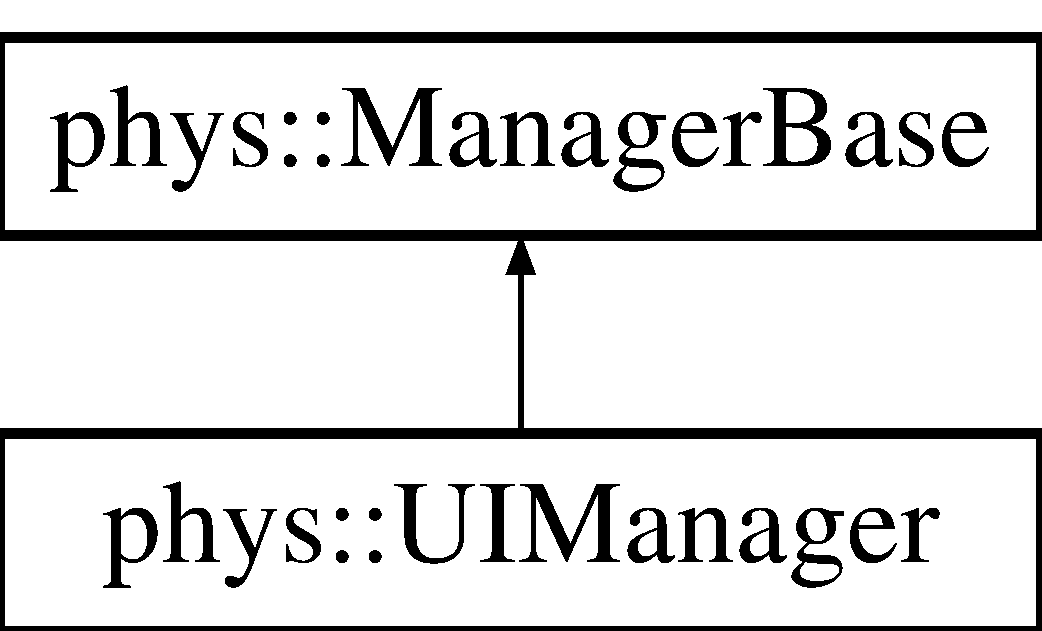
\includegraphics[height=2.000000cm]{d5/dc5/classphys_1_1UIManager}
\end{center}
\end{figure}
\subsection*{Public Member Functions}
\begin{DoxyCompactItemize}
\item 
\hyperlink{classphys_1_1UIManager_aeb502f11f170efd806b4153923c55359}{UIManager} ()
\begin{DoxyCompactList}\small\item\em Class Constructor. \item\end{DoxyCompactList}\item 
\hyperlink{classphys_1_1UIManager_a203144f08dbaf8068746359c22aa4f1e}{$\sim$UIManager} ()
\begin{DoxyCompactList}\small\item\em Class Destructor. \item\end{DoxyCompactList}\item 
\hypertarget{classphys_1_1UIManager_af04e60c4f09c114ec3bf32babdb64ab7}{
void \hyperlink{classphys_1_1UIManager_af04e60c4f09c114ec3bf32babdb64ab7}{Initialize} ()}
\label{d5/dc5/classphys_1_1UIManager_af04e60c4f09c114ec3bf32babdb64ab7}

\begin{DoxyCompactList}\small\item\em Inherited from \hyperlink{classphys_1_1ManagerBase}{ManagerBase}. \item\end{DoxyCompactList}\item 
\hypertarget{classphys_1_1UIManager_a972abedcd4343dc5966580f2f82494a8}{
void \hyperlink{classphys_1_1UIManager_a972abedcd4343dc5966580f2f82494a8}{DoMainLoopItems} ()}
\label{d5/dc5/classphys_1_1UIManager_a972abedcd4343dc5966580f2f82494a8}

\begin{DoxyCompactList}\small\item\em Inherited from \hyperlink{classphys_1_1ManagerBase}{ManagerBase}. \item\end{DoxyCompactList}\item 
void \hyperlink{classphys_1_1UIManager_afda4422105d6ab353fd40410adffbc0a}{LoadGorilla} (const \hyperlink{namespacephys_aa03900411993de7fbfec4789bc1d392e}{String} \&Name)
\begin{DoxyCompactList}\small\item\em Loads a Gorilla file for use with this manager. \item\end{DoxyCompactList}\item 
\hyperlink{classphys_1_1UI_1_1Button}{UI::Button} $\ast$ \hyperlink{classphys_1_1UIManager_acd08dba5be95182a6c923ed698822277}{GetHoveredButton} ()
\begin{DoxyCompactList}\small\item\em Gets the button the mouse is hovering over. \item\end{DoxyCompactList}\item 
\hyperlink{classphys_1_1UI_1_1Widget}{UI::Widget} $\ast$ \hyperlink{classphys_1_1UIManager_a5772b611b6881eb98932f4b400b44d09}{GetHoveredWidget} ()
\begin{DoxyCompactList}\small\item\em Gets the Widget the mouse is hovering over. \item\end{DoxyCompactList}\item 
\hyperlink{classphys_1_1UI_1_1Widget}{UI::Widget} $\ast$ \hyperlink{classphys_1_1UIManager_a99694297814d2e82ec507c6f4d6bec1a}{GetWidgetFocus} ()
\begin{DoxyCompactList}\small\item\em Gets the current widget being controlled. \item\end{DoxyCompactList}\item 
\hyperlink{classphys_1_1UIScreen}{UIScreen} $\ast$ \hyperlink{classphys_1_1UIManager_a7cad638d86489e03fa2599185514b58c}{CreateScreen} (const \hyperlink{namespacephys_aa03900411993de7fbfec4789bc1d392e}{String} \&Screen, const \hyperlink{namespacephys_aa03900411993de7fbfec4789bc1d392e}{String} \&Atlas, const \hyperlink{namespacephys_aa03900411993de7fbfec4789bc1d392e}{String} \&Viewport=\char`\"{}DefaultViewport\char`\"{})
\begin{DoxyCompactList}\small\item\em Creates an internal HUD screen. \item\end{DoxyCompactList}\item 
\hyperlink{classphys_1_1UIScreen}{UIScreen} $\ast$ \hyperlink{classphys_1_1UIManager_a8cd693c7ec9c458fcc4169eea0d7b4db}{GetScreen} (const \hyperlink{namespacephys_aa03900411993de7fbfec4789bc1d392e}{String} \&Name)
\begin{DoxyCompactList}\small\item\em Gets an already created screen by name. \item\end{DoxyCompactList}\item 
\hyperlink{classphys_1_1UIScreen}{UIScreen} $\ast$ \hyperlink{classphys_1_1UIManager_a6083b86b2e240cc316e8ca87479d15a8}{GetScreen} (\hyperlink{namespacephys_a460f6bc24c8dd347b05e0366ae34f34a}{Whole} Index)
\begin{DoxyCompactList}\small\item\em Gets an already created screen by index. \item\end{DoxyCompactList}\item 
\hyperlink{namespacephys_a460f6bc24c8dd347b05e0366ae34f34a}{Whole} \hyperlink{classphys_1_1UIManager_a3bd28c361f6fc79a182ebd3ec0a26ec7}{GetNumScreens} ()
\begin{DoxyCompactList}\small\item\em Gets the number of screens created and stored in this manager. \item\end{DoxyCompactList}\item 
void \hyperlink{classphys_1_1UIManager_a5afab78f58a6531fc18771f5a4eeccf8}{DestroyScreen} (\hyperlink{classphys_1_1UIScreen}{UIScreen} $\ast$Screen)
\begin{DoxyCompactList}\small\item\em Deletes a screen and removes all trace of it from the manager. \item\end{DoxyCompactList}\item 
\hypertarget{classphys_1_1UIManager_a97555e02aad6c85cac6bf67fbe074cd1}{
void \hyperlink{classphys_1_1UIManager_a97555e02aad6c85cac6bf67fbe074cd1}{DestroyAllScreens} ()}
\label{d5/dc5/classphys_1_1UIManager_a97555e02aad6c85cac6bf67fbe074cd1}

\begin{DoxyCompactList}\small\item\em Deletes all screens stored in this manager. \item\end{DoxyCompactList}\item 
\hyperlink{classphys_1_1UILayer}{UILayer} $\ast$ \hyperlink{classphys_1_1UIManager_ad80ed1716853f6e09cadc5f896e875e8}{GetLayer} (\hyperlink{namespacephys_aa03900411993de7fbfec4789bc1d392e}{String} \&Name)
\begin{DoxyCompactList}\small\item\em Searches all screens and gets the named Layer. \item\end{DoxyCompactList}\item 
\hyperlink{classphys_1_1UI_1_1Button}{UI::Button} $\ast$ \hyperlink{classphys_1_1UIManager_aa1022fcbe8e1efc7a383b2eff834a152}{CheckButtonMouseIsOver} ()
\begin{DoxyCompactList}\small\item\em Searches all visable screens and layers to see if a button was clicked. \item\end{DoxyCompactList}\item 
\hyperlink{classphys_1_1UI_1_1Widget}{UI::Widget} $\ast$ \hyperlink{classphys_1_1UIManager_ab9840b483409d3453a67931b4d858d1b}{CheckWidgetMouseIsOver} ()
\begin{DoxyCompactList}\small\item\em Searches all visable screens and layers to see if a widget was clicked. \item\end{DoxyCompactList}\item 
bool \hyperlink{classphys_1_1UIManager_a38bc8d2ed1930a8ff6e82ef5f991dbe1}{MouseIsInUISystem} ()
\begin{DoxyCompactList}\small\item\em Checks to see if the mouse is over a UI element. \item\end{DoxyCompactList}\item 
\hyperlink{classphys_1_1Vector2}{Vector2} \hyperlink{classphys_1_1UIManager_ae56846a64d8ce312aa36a749d15619df}{GetWindowDimensions} ()
\begin{DoxyCompactList}\small\item\em Gets the current window dimensions. \item\end{DoxyCompactList}\item 
\hyperlink{classphys_1_1InputQueryTool}{InputQueryTool} $\ast$ \hyperlink{classphys_1_1UIManager_a7b88d0fe2271cdceccf879eaba1b1a64}{GetInputQueryer} ()
\begin{DoxyCompactList}\small\item\em Gets the input queryer used for automation in this subsystem. \item\end{DoxyCompactList}\item 
\hyperlink{classphys_1_1ManagerBase_aaa6ccddf23892eaccb898529414f80a5}{ManagerBase::ManagerTypeName} \hyperlink{classphys_1_1UIManager_ab8fe74564ca5dc09cbe4b1cc2c007e79}{GetType} () const 
\begin{DoxyCompactList}\small\item\em Gets the type of manager that this manager is. \item\end{DoxyCompactList}\item 
Gorilla::Silverback $\ast$ \hyperlink{classphys_1_1UIManager_a21623edd39c3e23de29f4cf3ed6e490a}{GetSilverbackPointer} ()
\begin{DoxyCompactList}\small\item\em Gets the internal silverback pointer. \item\end{DoxyCompactList}\end{DoxyCompactItemize}
\subsection*{Protected Member Functions}
\begin{DoxyCompactItemize}
\item 
\hypertarget{classphys_1_1UIManager_ae5beaafe73c68d39eb84463033941057}{
void {\bfseries HoverChecks} ()}
\label{d5/dc5/classphys_1_1UIManager_ae5beaafe73c68d39eb84463033941057}

\item 
\hypertarget{classphys_1_1UIManager_aae0b6d575ea583154ca0257fb40d5ae7}{
void {\bfseries WidgetFocusUpdate} ()}
\label{d5/dc5/classphys_1_1UIManager_aae0b6d575ea583154ca0257fb40d5ae7}

\end{DoxyCompactItemize}
\subsection*{Protected Attributes}
\begin{DoxyCompactItemize}
\item 
\hypertarget{classphys_1_1UIManager_ab4c5b8c7e3c4c7b03847b1af18bea02a}{
Gorilla::Silverback $\ast$ \hyperlink{classphys_1_1UIManager_ab4c5b8c7e3c4c7b03847b1af18bea02a}{Silver}}
\label{d5/dc5/classphys_1_1UIManager_ab4c5b8c7e3c4c7b03847b1af18bea02a}

\begin{DoxyCompactList}\small\item\em Pointer for the Gorilla core class, where this manager gets it's functionality. \item\end{DoxyCompactList}\item 
\hypertarget{classphys_1_1UIManager_ab8eb94c63e1be1acda3891cd1862cc4e}{
std::vector$<$ \hyperlink{classphys_1_1UIScreen}{UIScreen} $\ast$ $>$ {\bfseries Screens}}
\label{d5/dc5/classphys_1_1UIManager_ab8eb94c63e1be1acda3891cd1862cc4e}

\item 
\hypertarget{classphys_1_1UIManager_a37293b9d9ba8b05c9a03e4640a56c6c1}{
\hyperlink{classphys_1_1UI_1_1Button}{UI::Button} $\ast$ {\bfseries HoveredButton}}
\label{d5/dc5/classphys_1_1UIManager_a37293b9d9ba8b05c9a03e4640a56c6c1}

\item 
\hypertarget{classphys_1_1UIManager_a3bcf192e061273695e99a85484c5056a}{
\hyperlink{classphys_1_1UI_1_1Widget}{UI::Widget} $\ast$ {\bfseries HoveredWidget}}
\label{d5/dc5/classphys_1_1UIManager_a3bcf192e061273695e99a85484c5056a}

\item 
\hypertarget{classphys_1_1UIManager_a932c928b9246717725c264326660bd6d}{
\hyperlink{classphys_1_1UI_1_1Widget}{UI::Widget} $\ast$ {\bfseries WidgetFocus}}
\label{d5/dc5/classphys_1_1UIManager_a932c928b9246717725c264326660bd6d}

\item 
\hypertarget{classphys_1_1UIManager_a0ae28b65bf930af50026f410b449d43b}{
\hyperlink{classphys_1_1InputQueryTool}{InputQueryTool} $\ast$ {\bfseries InputQueryer}}
\label{d5/dc5/classphys_1_1UIManager_a0ae28b65bf930af50026f410b449d43b}

\end{DoxyCompactItemize}


\subsection{Detailed Description}
This class is responsible for any and all user interactions with the User interface/HUD. Currently, you have to create the UI/HUD in code. Font and sprite data is loaded through a premade Gorilla file($\ast$.gorilla). 

Definition at line 74 of file uimanager.h.



\subsection{Constructor \& Destructor Documentation}
\hypertarget{classphys_1_1UIManager_aeb502f11f170efd806b4153923c55359}{
\index{phys::UIManager@{phys::UIManager}!UIManager@{UIManager}}
\index{UIManager@{UIManager}!phys::UIManager@{phys::UIManager}}
\subsubsection[{UIManager}]{\setlength{\rightskip}{0pt plus 5cm}phys::UIManager::UIManager (
\begin{DoxyParamCaption}
{}
\end{DoxyParamCaption}
)}}
\label{d5/dc5/classphys_1_1UIManager_aeb502f11f170efd806b4153923c55359}


Class Constructor. 

Standard class initialization constructor. 

Definition at line 59 of file uimanager.cpp.

\hypertarget{classphys_1_1UIManager_a203144f08dbaf8068746359c22aa4f1e}{
\index{phys::UIManager@{phys::UIManager}!$\sim$UIManager@{$\sim$UIManager}}
\index{$\sim$UIManager@{$\sim$UIManager}!phys::UIManager@{phys::UIManager}}
\subsubsection[{$\sim$UIManager}]{\setlength{\rightskip}{0pt plus 5cm}phys::UIManager::$\sim$UIManager (
\begin{DoxyParamCaption}
{}
\end{DoxyParamCaption}
)}}
\label{d5/dc5/classphys_1_1UIManager_a203144f08dbaf8068746359c22aa4f1e}


Class Destructor. 

The class destructor. 

Definition at line 69 of file uimanager.cpp.



\subsection{Member Function Documentation}
\hypertarget{classphys_1_1UIManager_aa1022fcbe8e1efc7a383b2eff834a152}{
\index{phys::UIManager@{phys::UIManager}!CheckButtonMouseIsOver@{CheckButtonMouseIsOver}}
\index{CheckButtonMouseIsOver@{CheckButtonMouseIsOver}!phys::UIManager@{phys::UIManager}}
\subsubsection[{CheckButtonMouseIsOver}]{\setlength{\rightskip}{0pt plus 5cm}{\bf UI::Button} $\ast$ phys::UIManager::CheckButtonMouseIsOver (
\begin{DoxyParamCaption}
{}
\end{DoxyParamCaption}
)}}
\label{d5/dc5/classphys_1_1UIManager_aa1022fcbe8e1efc7a383b2eff834a152}


Searches all visable screens and layers to see if a button was clicked. 

This is called automatically once every frame. Should only be called on manually if you need more then one check per frame. \begin{DoxyReturn}{Returns}
Returns the button clicked if there is one, NULL if not. 
\end{DoxyReturn}


Definition at line 229 of file uimanager.cpp.

\hypertarget{classphys_1_1UIManager_ab9840b483409d3453a67931b4d858d1b}{
\index{phys::UIManager@{phys::UIManager}!CheckWidgetMouseIsOver@{CheckWidgetMouseIsOver}}
\index{CheckWidgetMouseIsOver@{CheckWidgetMouseIsOver}!phys::UIManager@{phys::UIManager}}
\subsubsection[{CheckWidgetMouseIsOver}]{\setlength{\rightskip}{0pt plus 5cm}{\bf UI::Widget} $\ast$ phys::UIManager::CheckWidgetMouseIsOver (
\begin{DoxyParamCaption}
{}
\end{DoxyParamCaption}
)}}
\label{d5/dc5/classphys_1_1UIManager_ab9840b483409d3453a67931b4d858d1b}


Searches all visable screens and layers to see if a widget was clicked. 

This is called automatically once every frame. Should only be called on manually if you need more then one check per frame. \begin{DoxyReturn}{Returns}
Returns the widget clicked if there is one, NULL if not. 
\end{DoxyReturn}


Definition at line 245 of file uimanager.cpp.

\hypertarget{classphys_1_1UIManager_a7cad638d86489e03fa2599185514b58c}{
\index{phys::UIManager@{phys::UIManager}!CreateScreen@{CreateScreen}}
\index{CreateScreen@{CreateScreen}!phys::UIManager@{phys::UIManager}}
\subsubsection[{CreateScreen}]{\setlength{\rightskip}{0pt plus 5cm}{\bf UIScreen} $\ast$ phys::UIManager::CreateScreen (
\begin{DoxyParamCaption}
\item[{const {\bf String} \&}]{ Screen, }
\item[{const {\bf String} \&}]{ Atlas, }
\item[{const {\bf String} \&}]{ Viewport = {\ttfamily \char`\"{}DefaultViewport\char`\"{}}}
\end{DoxyParamCaption}
)}}
\label{d5/dc5/classphys_1_1UIManager_a7cad638d86489e03fa2599185514b58c}


Creates an internal HUD screen. 

Screens are the base set of renderable UI you can use, allowing you to switch entire sets of UI's on the fly if needed. For performance reasons you should always keep the number of screens you create to a minimum. 
\begin{DoxyParams}{Parameters}
\item[{\em Screen}]The name to be given to the screen. \item[{\em Atlas}]The name of a previously loaded Gorilla file to be used with this screen. \item[{\em Viewport}]The name of the viewport to create this screen in. \end{DoxyParams}


Definition at line 158 of file uimanager.cpp.

\hypertarget{classphys_1_1UIManager_a5afab78f58a6531fc18771f5a4eeccf8}{
\index{phys::UIManager@{phys::UIManager}!DestroyScreen@{DestroyScreen}}
\index{DestroyScreen@{DestroyScreen}!phys::UIManager@{phys::UIManager}}
\subsubsection[{DestroyScreen}]{\setlength{\rightskip}{0pt plus 5cm}void phys::UIManager::DestroyScreen (
\begin{DoxyParamCaption}
\item[{{\bf UIScreen} $\ast$}]{ Screen}
\end{DoxyParamCaption}
)}}
\label{d5/dc5/classphys_1_1UIManager_a5afab78f58a6531fc18771f5a4eeccf8}


Deletes a screen and removes all trace of it from the manager. 

Destroying a screen will also destroy all of it's layers, and everything contained in those layers. 
\begin{DoxyParams}{Parameters}
\item[{\em Screen}]The screen to be destroyed. \end{DoxyParams}


Definition at line 191 of file uimanager.cpp.

\hypertarget{classphys_1_1UIManager_acd08dba5be95182a6c923ed698822277}{
\index{phys::UIManager@{phys::UIManager}!GetHoveredButton@{GetHoveredButton}}
\index{GetHoveredButton@{GetHoveredButton}!phys::UIManager@{phys::UIManager}}
\subsubsection[{GetHoveredButton}]{\setlength{\rightskip}{0pt plus 5cm}{\bf UI::Button} $\ast$ phys::UIManager::GetHoveredButton (
\begin{DoxyParamCaption}
{}
\end{DoxyParamCaption}
)}}
\label{d5/dc5/classphys_1_1UIManager_acd08dba5be95182a6c923ed698822277}


Gets the button the mouse is hovering over. 

This check will look through both standalone buttons and widget buttons. \begin{DoxyReturn}{Returns}
Returns a pointer to the button, or NULL if it's not over any visable buttons. 
\end{DoxyReturn}


Definition at line 143 of file uimanager.cpp.

\hypertarget{classphys_1_1UIManager_a5772b611b6881eb98932f4b400b44d09}{
\index{phys::UIManager@{phys::UIManager}!GetHoveredWidget@{GetHoveredWidget}}
\index{GetHoveredWidget@{GetHoveredWidget}!phys::UIManager@{phys::UIManager}}
\subsubsection[{GetHoveredWidget}]{\setlength{\rightskip}{0pt plus 5cm}{\bf UI::Widget} $\ast$ phys::UIManager::GetHoveredWidget (
\begin{DoxyParamCaption}
{}
\end{DoxyParamCaption}
)}}
\label{d5/dc5/classphys_1_1UIManager_a5772b611b6881eb98932f4b400b44d09}


Gets the Widget the mouse is hovering over. 

If the widget found during widget checks belongs to a widget, this will get that widget. \begin{DoxyReturn}{Returns}
Returns a pointer to the widget, or NULL if it's not over any visable buttons. 
\end{DoxyReturn}


Definition at line 148 of file uimanager.cpp.

\hypertarget{classphys_1_1UIManager_a7b88d0fe2271cdceccf879eaba1b1a64}{
\index{phys::UIManager@{phys::UIManager}!GetInputQueryer@{GetInputQueryer}}
\index{GetInputQueryer@{GetInputQueryer}!phys::UIManager@{phys::UIManager}}
\subsubsection[{GetInputQueryer}]{\setlength{\rightskip}{0pt plus 5cm}{\bf InputQueryTool} $\ast$ phys::UIManager::GetInputQueryer (
\begin{DoxyParamCaption}
{}
\end{DoxyParamCaption}
)}}
\label{d5/dc5/classphys_1_1UIManager_a7b88d0fe2271cdceccf879eaba1b1a64}


Gets the input queryer used for automation in this subsystem. 

\begin{DoxyReturn}{Returns}
Returns a pointer to the \hyperlink{classphys_1_1InputQueryTool}{InputQueryTool} used to query input events for this subsystem. 
\end{DoxyReturn}


Definition at line 280 of file uimanager.cpp.

\hypertarget{classphys_1_1UIManager_ad80ed1716853f6e09cadc5f896e875e8}{
\index{phys::UIManager@{phys::UIManager}!GetLayer@{GetLayer}}
\index{GetLayer@{GetLayer}!phys::UIManager@{phys::UIManager}}
\subsubsection[{GetLayer}]{\setlength{\rightskip}{0pt plus 5cm}{\bf UILayer} $\ast$ phys::UIManager::GetLayer (
\begin{DoxyParamCaption}
\item[{{\bf String} \&}]{ Name}
\end{DoxyParamCaption}
)}}
\label{d5/dc5/classphys_1_1UIManager_ad80ed1716853f6e09cadc5f896e875e8}


Searches all screens and gets the named Layer. 

\begin{DoxyReturn}{Returns}
Returns the named layer if found, NULL if not. 
\end{DoxyReturn}


Definition at line 218 of file uimanager.cpp.

\hypertarget{classphys_1_1UIManager_a3bd28c361f6fc79a182ebd3ec0a26ec7}{
\index{phys::UIManager@{phys::UIManager}!GetNumScreens@{GetNumScreens}}
\index{GetNumScreens@{GetNumScreens}!phys::UIManager@{phys::UIManager}}
\subsubsection[{GetNumScreens}]{\setlength{\rightskip}{0pt plus 5cm}{\bf Whole} phys::UIManager::GetNumScreens (
\begin{DoxyParamCaption}
{}
\end{DoxyParamCaption}
)}}
\label{d5/dc5/classphys_1_1UIManager_a3bd28c361f6fc79a182ebd3ec0a26ec7}


Gets the number of screens created and stored in this manager. 

\begin{DoxyReturn}{Returns}
Returns the number of screens this manager is storing. 
\end{DoxyReturn}


Definition at line 186 of file uimanager.cpp.

\hypertarget{classphys_1_1UIManager_a8cd693c7ec9c458fcc4169eea0d7b4db}{
\index{phys::UIManager@{phys::UIManager}!GetScreen@{GetScreen}}
\index{GetScreen@{GetScreen}!phys::UIManager@{phys::UIManager}}
\subsubsection[{GetScreen}]{\setlength{\rightskip}{0pt plus 5cm}{\bf UIScreen} $\ast$ phys::UIManager::GetScreen (
\begin{DoxyParamCaption}
\item[{const {\bf String} \&}]{ Name}
\end{DoxyParamCaption}
)}}
\label{d5/dc5/classphys_1_1UIManager_a8cd693c7ec9c458fcc4169eea0d7b4db}


Gets an already created screen by name. 

\begin{DoxyReturn}{Returns}
Returns a pointer to the screen of the specified name. 
\end{DoxyReturn}


Definition at line 167 of file uimanager.cpp.

\hypertarget{classphys_1_1UIManager_a6083b86b2e240cc316e8ca87479d15a8}{
\index{phys::UIManager@{phys::UIManager}!GetScreen@{GetScreen}}
\index{GetScreen@{GetScreen}!phys::UIManager@{phys::UIManager}}
\subsubsection[{GetScreen}]{\setlength{\rightskip}{0pt plus 5cm}{\bf UIScreen} $\ast$ phys::UIManager::GetScreen (
\begin{DoxyParamCaption}
\item[{{\bf Whole}}]{ Index}
\end{DoxyParamCaption}
)}}
\label{d5/dc5/classphys_1_1UIManager_a6083b86b2e240cc316e8ca87479d15a8}


Gets an already created screen by index. 

\begin{DoxyReturn}{Returns}
Returns a pointer to the screen at the specified index. 
\end{DoxyReturn}


Definition at line 181 of file uimanager.cpp.

\hypertarget{classphys_1_1UIManager_a21623edd39c3e23de29f4cf3ed6e490a}{
\index{phys::UIManager@{phys::UIManager}!GetSilverbackPointer@{GetSilverbackPointer}}
\index{GetSilverbackPointer@{GetSilverbackPointer}!phys::UIManager@{phys::UIManager}}
\subsubsection[{GetSilverbackPointer}]{\setlength{\rightskip}{0pt plus 5cm}Gorilla::Silverback $\ast$ phys::UIManager::GetSilverbackPointer (
\begin{DoxyParamCaption}
{}
\end{DoxyParamCaption}
)}}
\label{d5/dc5/classphys_1_1UIManager_a21623edd39c3e23de29f4cf3ed6e490a}


Gets the internal silverback pointer. 

\begin{DoxyInternal}{For internal use only.}
\begin{DoxyReturn}{Returns}
Returns a pointer to the internal silverback class. 
\end{DoxyReturn}
\end{DoxyInternal}


Definition at line 288 of file uimanager.cpp.

\hypertarget{classphys_1_1UIManager_ab8fe74564ca5dc09cbe4b1cc2c007e79}{
\index{phys::UIManager@{phys::UIManager}!GetType@{GetType}}
\index{GetType@{GetType}!phys::UIManager@{phys::UIManager}}
\subsubsection[{GetType}]{\setlength{\rightskip}{0pt plus 5cm}{\bf ManagerBase::ManagerTypeName} phys::UIManager::GetType (
\begin{DoxyParamCaption}
{}
\end{DoxyParamCaption}
) const\hspace{0.3cm}{\ttfamily  \mbox{[}virtual\mbox{]}}}}
\label{d5/dc5/classphys_1_1UIManager_ab8fe74564ca5dc09cbe4b1cc2c007e79}


Gets the type of manager that this manager is. 

\begin{DoxyReturn}{Returns}
Returns an enum value representing the type of manager that this manager is. 
\end{DoxyReturn}


Implements \hyperlink{classphys_1_1ManagerBase_aff400b6599db635e24796d8221e9a0e3}{phys::ManagerBase}.



Definition at line 285 of file uimanager.cpp.

\hypertarget{classphys_1_1UIManager_a99694297814d2e82ec507c6f4d6bec1a}{
\index{phys::UIManager@{phys::UIManager}!GetWidgetFocus@{GetWidgetFocus}}
\index{GetWidgetFocus@{GetWidgetFocus}!phys::UIManager@{phys::UIManager}}
\subsubsection[{GetWidgetFocus}]{\setlength{\rightskip}{0pt plus 5cm}{\bf UI::Widget} $\ast$ phys::UIManager::GetWidgetFocus (
\begin{DoxyParamCaption}
{}
\end{DoxyParamCaption}
)}}
\label{d5/dc5/classphys_1_1UIManager_a99694297814d2e82ec507c6f4d6bec1a}


Gets the current widget being controlled. 

The widget control is used mostly for manipulating widgets while the mouse is not currently hovering over them, such as the click and drag action of scrollbars and resizing windows. \begin{DoxyReturn}{Returns}
Returns a pointer to the currently controlled widget, or NULL if none are being controlled this frame. 
\end{DoxyReturn}


Definition at line 153 of file uimanager.cpp.

\hypertarget{classphys_1_1UIManager_ae56846a64d8ce312aa36a749d15619df}{
\index{phys::UIManager@{phys::UIManager}!GetWindowDimensions@{GetWindowDimensions}}
\index{GetWindowDimensions@{GetWindowDimensions}!phys::UIManager@{phys::UIManager}}
\subsubsection[{GetWindowDimensions}]{\setlength{\rightskip}{0pt plus 5cm}{\bf Vector2} phys::UIManager::GetWindowDimensions (
\begin{DoxyParamCaption}
{}
\end{DoxyParamCaption}
)}}
\label{d5/dc5/classphys_1_1UIManager_ae56846a64d8ce312aa36a749d15619df}


Gets the current window dimensions. 

\begin{DoxyReturn}{Returns}
Returns a \hyperlink{classphys_1_1Vector2}{Vector2} representing the current window dimensions. 
\end{DoxyReturn}


\begin{Desc}
\item[\hyperlink{todo__todo000027}{Todo}]This is the second occurance of needing to specify the namespace to declare data without any apparent reason. If possible a pattern/explaination should be found. \end{Desc}




Definition at line 271 of file uimanager.cpp.

\hypertarget{classphys_1_1UIManager_afda4422105d6ab353fd40410adffbc0a}{
\index{phys::UIManager@{phys::UIManager}!LoadGorilla@{LoadGorilla}}
\index{LoadGorilla@{LoadGorilla}!phys::UIManager@{phys::UIManager}}
\subsubsection[{LoadGorilla}]{\setlength{\rightskip}{0pt plus 5cm}void phys::UIManager::LoadGorilla (
\begin{DoxyParamCaption}
\item[{const {\bf String} \&}]{ Name}
\end{DoxyParamCaption}
)}}
\label{d5/dc5/classphys_1_1UIManager_afda4422105d6ab353fd40410adffbc0a}


Loads a Gorilla file for use with this manager. 


\begin{DoxyParams}{Parameters}
\item[{\em Name}]The name of the file to be loaded, not including the extension. \end{DoxyParams}


Definition at line 138 of file uimanager.cpp.

\hypertarget{classphys_1_1UIManager_a38bc8d2ed1930a8ff6e82ef5f991dbe1}{
\index{phys::UIManager@{phys::UIManager}!MouseIsInUISystem@{MouseIsInUISystem}}
\index{MouseIsInUISystem@{MouseIsInUISystem}!phys::UIManager@{phys::UIManager}}
\subsubsection[{MouseIsInUISystem}]{\setlength{\rightskip}{0pt plus 5cm}bool phys::UIManager::MouseIsInUISystem (
\begin{DoxyParamCaption}
{}
\end{DoxyParamCaption}
)}}
\label{d5/dc5/classphys_1_1UIManager_a38bc8d2ed1930a8ff6e82ef5f991dbe1}


Checks to see if the mouse is over a UI element. 

This should only be called on after this manager does it's main loop items for best results. \begin{DoxyReturn}{Returns}
Returns true if the mouse is over a visable UI element, false if not. 
\end{DoxyReturn}


Definition at line 261 of file uimanager.cpp.



The documentation for this class was generated from the following files:\begin{DoxyCompactItemize}
\item 
uimanager.h\item 
uimanager.cpp\end{DoxyCompactItemize}

\hypertarget{classphys_1_1UIScreen}{
\section{phys::UIScreen Class Reference}
\label{d9/de8/classphys_1_1UIScreen}\index{phys::UIScreen@{phys::UIScreen}}
}


This class is a helper class for creating UI's. It is responsible for storing and keeping track of all the elements of a single UI screen.  




{\ttfamily \#include $<$uiscreen.h$>$}

\subsection*{Public Member Functions}
\begin{DoxyCompactItemize}
\item 
\hyperlink{classphys_1_1UIScreen_a721e1743b3f09e0112ff512d2888737c}{UIScreen} (const \hyperlink{namespacephys_aa03900411993de7fbfec4789bc1d392e}{String} \&name, Gorilla::Screen $\ast$GScreen)
\begin{DoxyCompactList}\small\item\em Internal constructor. \item\end{DoxyCompactList}\item 
\hypertarget{classphys_1_1UIScreen_a5b8d4ebcffefeac1b39b6dac5a51b650}{
\hyperlink{classphys_1_1UIScreen_a5b8d4ebcffefeac1b39b6dac5a51b650}{$\sim$UIScreen} ()}
\label{d9/de8/classphys_1_1UIScreen_a5b8d4ebcffefeac1b39b6dac5a51b650}

\begin{DoxyCompactList}\small\item\em Class destructor. \item\end{DoxyCompactList}\item 
\hyperlink{namespacephys_aa03900411993de7fbfec4789bc1d392e}{String} \& \hyperlink{classphys_1_1UIScreen_aee363edcdc7d21197e4103668011f8fb}{GetName} ()
\begin{DoxyCompactList}\small\item\em Gets the name of this screen. \item\end{DoxyCompactList}\item 
void \hyperlink{classphys_1_1UIScreen_ac8b143b35fd96e9aed694089d2732396}{SetVisible} (bool Visible)
\begin{DoxyCompactList}\small\item\em Sets the screens visability. \item\end{DoxyCompactList}\item 
bool \hyperlink{classphys_1_1UIScreen_a8f64052f7bb0b6be2f55c73f31bfea29}{IsVisible} ()
\begin{DoxyCompactList}\small\item\em Gets the screens visability. \item\end{DoxyCompactList}\item 
\hypertarget{classphys_1_1UIScreen_a0ba9ce016f7da06ab73fa2abea134a18}{
void \hyperlink{classphys_1_1UIScreen_a0ba9ce016f7da06ab73fa2abea134a18}{Show} ()}
\label{d9/de8/classphys_1_1UIScreen_a0ba9ce016f7da06ab73fa2abea134a18}

\begin{DoxyCompactList}\small\item\em Forces the screen to be shown. \item\end{DoxyCompactList}\item 
\hypertarget{classphys_1_1UIScreen_af9ea18cf145e31b90dbe02faed758343}{
void \hyperlink{classphys_1_1UIScreen_af9ea18cf145e31b90dbe02faed758343}{Hide} ()}
\label{d9/de8/classphys_1_1UIScreen_af9ea18cf145e31b90dbe02faed758343}

\begin{DoxyCompactList}\small\item\em Forces the screen to hide. \item\end{DoxyCompactList}\item 
\hyperlink{classphys_1_1UILayer}{UILayer} $\ast$ \hyperlink{classphys_1_1UIScreen_a14c3256bda81d40553ff065993fcbe77}{CreateLayer} (const \hyperlink{namespacephys_aa03900411993de7fbfec4789bc1d392e}{String} \&Name, \hyperlink{namespacephys_a460f6bc24c8dd347b05e0366ae34f34a}{Whole} Zorder)
\begin{DoxyCompactList}\small\item\em Creates a layer in the GUI screen to place GUI objects in. \item\end{DoxyCompactList}\item 
\hyperlink{classphys_1_1UILayer}{UILayer} $\ast$ \hyperlink{classphys_1_1UIScreen_a661f461325f3a67169ce0c4ee107c8eb}{GetLayer} (const \hyperlink{namespacephys_aa03900411993de7fbfec4789bc1d392e}{String} \&Name)
\begin{DoxyCompactList}\small\item\em Gets an already created layer by name. \item\end{DoxyCompactList}\item 
\hyperlink{classphys_1_1UILayer}{UILayer} $\ast$ \hyperlink{classphys_1_1UIScreen_a8b9aeb4599c47d2b4ea0a1c5d5e6f210}{GetLayer} (\hyperlink{namespacephys_a460f6bc24c8dd347b05e0366ae34f34a}{Whole} Index)
\begin{DoxyCompactList}\small\item\em Gets an already created layer by it's index. \item\end{DoxyCompactList}\item 
\hyperlink{classphys_1_1UILayer}{UILayer} $\ast$ \hyperlink{classphys_1_1UIScreen_ab558b5405a1f64d7558e34a217bfc28d}{GetLayerbyZorder} (\hyperlink{namespacephys_a460f6bc24c8dd347b05e0366ae34f34a}{Whole} Zorder)
\begin{DoxyCompactList}\small\item\em Gets an already created layer by it's Zorder. \item\end{DoxyCompactList}\item 
\hyperlink{namespacephys_a460f6bc24c8dd347b05e0366ae34f34a}{Whole} \hyperlink{classphys_1_1UIScreen_a87c4cf832f36af0182483814fec30f88}{GetNumLayers} ()
\begin{DoxyCompactList}\small\item\em Gets the number of layers created and stored in this class. \item\end{DoxyCompactList}\item 
void \hyperlink{classphys_1_1UIScreen_ac1d9dfc0b8d9b3720f1447dcc93d8b55}{DestroyLayer} (\hyperlink{classphys_1_1UILayer}{UILayer} $\ast$Layer)
\begin{DoxyCompactList}\small\item\em Destroy's a previously created layer. \item\end{DoxyCompactList}\item 
\hyperlink{classphys_1_1UI_1_1Button}{UI::Button} $\ast$ \hyperlink{classphys_1_1UIScreen_a7bc1a10b2172ad8885901de1a65a819d}{CheckButtonMouseIsOver} ()
\begin{DoxyCompactList}\small\item\em Gets the button the mouse is over if any. \item\end{DoxyCompactList}\item 
\hyperlink{classphys_1_1UI_1_1Widget}{UI::Widget} $\ast$ \hyperlink{classphys_1_1UIScreen_a00befef8c7bce9e8d149e6ba03419a53}{CheckWidgetMouseIsOver} ()
\begin{DoxyCompactList}\small\item\em Gets the widget the mouse is over if any. \item\end{DoxyCompactList}\item 
Gorilla::Screen $\ast$ \hyperlink{classphys_1_1UIScreen_a1ec3a329f7864905e6dc387f469068df}{GetGorillaScreen} ()
\begin{DoxyCompactList}\small\item\em Gets the internal screen this screen is based on. \item\end{DoxyCompactList}\end{DoxyCompactItemize}
\subsection*{Protected Attributes}
\begin{DoxyCompactItemize}
\item 
\hypertarget{classphys_1_1UIScreen_a6cc0cb1a19c2b2a8cee20222d1af333c}{
Gorilla::Screen $\ast$ {\bfseries GorillaScreen}}
\label{d9/de8/classphys_1_1UIScreen_a6cc0cb1a19c2b2a8cee20222d1af333c}

\item 
\hypertarget{classphys_1_1UIScreen_a8cb86a27b0ac39426ae23e67e34ebd47}{
\hyperlink{classphys_1_1UIManager}{UIManager} $\ast$ {\bfseries Manager}}
\label{d9/de8/classphys_1_1UIScreen_a8cb86a27b0ac39426ae23e67e34ebd47}

\item 
\hypertarget{classphys_1_1UIScreen_a513aebb318ba6e21fcc95090c4385614}{
\hyperlink{namespacephys_aa03900411993de7fbfec4789bc1d392e}{String} {\bfseries Name}}
\label{d9/de8/classphys_1_1UIScreen_a513aebb318ba6e21fcc95090c4385614}

\item 
\hypertarget{classphys_1_1UIScreen_aab6876d055853ed554e1ab09d0e91ce0}{
std::map$<$ \hyperlink{namespacephys_a460f6bc24c8dd347b05e0366ae34f34a}{Whole}, \hyperlink{classphys_1_1UILayer}{UILayer} $\ast$ $>$ {\bfseries Layers}}
\label{d9/de8/classphys_1_1UIScreen_aab6876d055853ed554e1ab09d0e91ce0}

\end{DoxyCompactItemize}


\subsection{Detailed Description}
This class is a helper class for creating UI's. It is responsible for storing and keeping track of all the elements of a single UI screen. UI's can optionally be divided up into Screens, or \char`\"{}pages\char`\"{}. Each screen is batched together for rendering, so keeping the amount of screens to a minimum will improve performance. 

Definition at line 71 of file uiscreen.h.



\subsection{Constructor \& Destructor Documentation}
\hypertarget{classphys_1_1UIScreen_a721e1743b3f09e0112ff512d2888737c}{
\index{phys::UIScreen@{phys::UIScreen}!UIScreen@{UIScreen}}
\index{UIScreen@{UIScreen}!phys::UIScreen@{phys::UIScreen}}
\subsubsection[{UIScreen}]{\setlength{\rightskip}{0pt plus 5cm}phys::UIScreen::UIScreen (
\begin{DoxyParamCaption}
\item[{const {\bf String} \&}]{ name, }
\item[{Gorilla::Screen $\ast$}]{ GScreen}
\end{DoxyParamCaption}
)}}
\label{d9/de8/classphys_1_1UIScreen_a721e1743b3f09e0112ff512d2888737c}


Internal constructor. 


\begin{DoxyParams}{Parameters}
\item[{\em GScreen}]The Gorilla Screen this Screen is based on. \item[{\em manager}]Pointer to the manager that created this Screen. \end{DoxyParams}


Definition at line 52 of file uiscreen.cpp.



\subsection{Member Function Documentation}
\hypertarget{classphys_1_1UIScreen_a7bc1a10b2172ad8885901de1a65a819d}{
\index{phys::UIScreen@{phys::UIScreen}!CheckButtonMouseIsOver@{CheckButtonMouseIsOver}}
\index{CheckButtonMouseIsOver@{CheckButtonMouseIsOver}!phys::UIScreen@{phys::UIScreen}}
\subsubsection[{CheckButtonMouseIsOver}]{\setlength{\rightskip}{0pt plus 5cm}{\bf UI::Button} $\ast$ phys::UIScreen::CheckButtonMouseIsOver (
\begin{DoxyParamCaption}
{}
\end{DoxyParamCaption}
)}}
\label{d9/de8/classphys_1_1UIScreen_a7bc1a10b2172ad8885901de1a65a819d}


Gets the button the mouse is over if any. 

This function searches only the visable layers contained in this screen. \begin{DoxyReturn}{Returns}
Returns the button the mouse is over, or NULL if there are none. 
\end{DoxyReturn}


Definition at line 157 of file uiscreen.cpp.

\hypertarget{classphys_1_1UIScreen_a00befef8c7bce9e8d149e6ba03419a53}{
\index{phys::UIScreen@{phys::UIScreen}!CheckWidgetMouseIsOver@{CheckWidgetMouseIsOver}}
\index{CheckWidgetMouseIsOver@{CheckWidgetMouseIsOver}!phys::UIScreen@{phys::UIScreen}}
\subsubsection[{CheckWidgetMouseIsOver}]{\setlength{\rightskip}{0pt plus 5cm}{\bf UI::Widget} $\ast$ phys::UIScreen::CheckWidgetMouseIsOver (
\begin{DoxyParamCaption}
{}
\end{DoxyParamCaption}
)}}
\label{d9/de8/classphys_1_1UIScreen_a00befef8c7bce9e8d149e6ba03419a53}


Gets the widget the mouse is over if any. 

This function searches only the visable layers contained in this screen. \begin{DoxyReturn}{Returns}
Returns the widget the mouse is over, or NULL if there are none. 
\end{DoxyReturn}


Definition at line 173 of file uiscreen.cpp.

\hypertarget{classphys_1_1UIScreen_a14c3256bda81d40553ff065993fcbe77}{
\index{phys::UIScreen@{phys::UIScreen}!CreateLayer@{CreateLayer}}
\index{CreateLayer@{CreateLayer}!phys::UIScreen@{phys::UIScreen}}
\subsubsection[{CreateLayer}]{\setlength{\rightskip}{0pt plus 5cm}{\bf UILayer} $\ast$ phys::UIScreen::CreateLayer (
\begin{DoxyParamCaption}
\item[{const {\bf String} \&}]{ Name, }
\item[{{\bf Whole}}]{ Zorder}
\end{DoxyParamCaption}
)}}
\label{d9/de8/classphys_1_1UIScreen_a14c3256bda81d40553ff065993fcbe77}


Creates a layer in the GUI screen to place GUI objects in. 

A GUI layer is exactly that, a layer of GUI objects. You can have multiple GUI layers per screen. The Zorder of the layer determines it's visability if there are multiple layers. If the Zorder of one layer is higher then another in the same space, then the Zorder with the higher Zorder will be rendered...giving it the appearance of being on top of the other GUI object or objects. 
\begin{DoxyParams}{Parameters}
\item[{\em Name}]The name to be given to the layer. \item[{\em Zorder}]The layers Zorder, as explained above. \end{DoxyParams}


\begin{Desc}
\item[\hyperlink{todo__todo000029}{Todo}]add an exception here or maybe log entry, some notification it failed. \end{Desc}




Definition at line 89 of file uiscreen.cpp.

\hypertarget{classphys_1_1UIScreen_ac1d9dfc0b8d9b3720f1447dcc93d8b55}{
\index{phys::UIScreen@{phys::UIScreen}!DestroyLayer@{DestroyLayer}}
\index{DestroyLayer@{DestroyLayer}!phys::UIScreen@{phys::UIScreen}}
\subsubsection[{DestroyLayer}]{\setlength{\rightskip}{0pt plus 5cm}void phys::UIScreen::DestroyLayer (
\begin{DoxyParamCaption}
\item[{{\bf UILayer} $\ast$}]{ Layer}
\end{DoxyParamCaption}
)}}
\label{d9/de8/classphys_1_1UIScreen_ac1d9dfc0b8d9b3720f1447dcc93d8b55}


Destroy's a previously created layer. 


\begin{DoxyParams}{Parameters}
\item[{\em Name}]The name of the layer to be destroyed. \end{DoxyParams}


Definition at line 142 of file uiscreen.cpp.

\hypertarget{classphys_1_1UIScreen_a1ec3a329f7864905e6dc387f469068df}{
\index{phys::UIScreen@{phys::UIScreen}!GetGorillaScreen@{GetGorillaScreen}}
\index{GetGorillaScreen@{GetGorillaScreen}!phys::UIScreen@{phys::UIScreen}}
\subsubsection[{GetGorillaScreen}]{\setlength{\rightskip}{0pt plus 5cm}Gorilla::Screen $\ast$ phys::UIScreen::GetGorillaScreen (
\begin{DoxyParamCaption}
{}
\end{DoxyParamCaption}
)}}
\label{d9/de8/classphys_1_1UIScreen_a1ec3a329f7864905e6dc387f469068df}


Gets the internal screen this screen is based on. 

\begin{DoxyInternal}{For internal use only.}
\begin{DoxyReturn}{Returns}
Returns a pointer to the Gorilla screen this screen is based on. 
\end{DoxyReturn}
\end{DoxyInternal}


Definition at line 189 of file uiscreen.cpp.

\hypertarget{classphys_1_1UIScreen_a8b9aeb4599c47d2b4ea0a1c5d5e6f210}{
\index{phys::UIScreen@{phys::UIScreen}!GetLayer@{GetLayer}}
\index{GetLayer@{GetLayer}!phys::UIScreen@{phys::UIScreen}}
\subsubsection[{GetLayer}]{\setlength{\rightskip}{0pt plus 5cm}{\bf UILayer} $\ast$ phys::UIScreen::GetLayer (
\begin{DoxyParamCaption}
\item[{{\bf Whole}}]{ Index}
\end{DoxyParamCaption}
)}}
\label{d9/de8/classphys_1_1UIScreen_a8b9aeb4599c47d2b4ea0a1c5d5e6f210}


Gets an already created layer by it's index. 

\begin{DoxyReturn}{Returns}
Returns a pointer to the layer at the specified index. 
\end{DoxyReturn}


Definition at line 116 of file uiscreen.cpp.

\hypertarget{classphys_1_1UIScreen_a661f461325f3a67169ce0c4ee107c8eb}{
\index{phys::UIScreen@{phys::UIScreen}!GetLayer@{GetLayer}}
\index{GetLayer@{GetLayer}!phys::UIScreen@{phys::UIScreen}}
\subsubsection[{GetLayer}]{\setlength{\rightskip}{0pt plus 5cm}{\bf UILayer} $\ast$ phys::UIScreen::GetLayer (
\begin{DoxyParamCaption}
\item[{const {\bf String} \&}]{ Name}
\end{DoxyParamCaption}
)}}
\label{d9/de8/classphys_1_1UIScreen_a661f461325f3a67169ce0c4ee107c8eb}


Gets an already created layer by name. 

\begin{DoxyReturn}{Returns}
Returns a pointer to the layer of the specified name. 
\end{DoxyReturn}


Definition at line 103 of file uiscreen.cpp.

\hypertarget{classphys_1_1UIScreen_ab558b5405a1f64d7558e34a217bfc28d}{
\index{phys::UIScreen@{phys::UIScreen}!GetLayerbyZorder@{GetLayerbyZorder}}
\index{GetLayerbyZorder@{GetLayerbyZorder}!phys::UIScreen@{phys::UIScreen}}
\subsubsection[{GetLayerbyZorder}]{\setlength{\rightskip}{0pt plus 5cm}{\bf UILayer} $\ast$ phys::UIScreen::GetLayerbyZorder (
\begin{DoxyParamCaption}
\item[{{\bf Whole}}]{ Zorder}
\end{DoxyParamCaption}
)}}
\label{d9/de8/classphys_1_1UIScreen_ab558b5405a1f64d7558e34a217bfc28d}


Gets an already created layer by it's Zorder. 

\begin{DoxyReturn}{Returns}
Returns a pointer to the layer with the specified Zorder. 
\end{DoxyReturn}


Definition at line 129 of file uiscreen.cpp.

\hypertarget{classphys_1_1UIScreen_aee363edcdc7d21197e4103668011f8fb}{
\index{phys::UIScreen@{phys::UIScreen}!GetName@{GetName}}
\index{GetName@{GetName}!phys::UIScreen@{phys::UIScreen}}
\subsubsection[{GetName}]{\setlength{\rightskip}{0pt plus 5cm}{\bf String} \& phys::UIScreen::GetName (
\begin{DoxyParamCaption}
{}
\end{DoxyParamCaption}
)}}
\label{d9/de8/classphys_1_1UIScreen_aee363edcdc7d21197e4103668011f8fb}


Gets the name of this screen. 

\begin{DoxyReturn}{Returns}
Returns a string containing the name of this screen. 
\end{DoxyReturn}


Definition at line 64 of file uiscreen.cpp.

\hypertarget{classphys_1_1UIScreen_a87c4cf832f36af0182483814fec30f88}{
\index{phys::UIScreen@{phys::UIScreen}!GetNumLayers@{GetNumLayers}}
\index{GetNumLayers@{GetNumLayers}!phys::UIScreen@{phys::UIScreen}}
\subsubsection[{GetNumLayers}]{\setlength{\rightskip}{0pt plus 5cm}{\bf Whole} phys::UIScreen::GetNumLayers (
\begin{DoxyParamCaption}
{}
\end{DoxyParamCaption}
)}}
\label{d9/de8/classphys_1_1UIScreen_a87c4cf832f36af0182483814fec30f88}


Gets the number of layers created and stored in this class. 

\begin{DoxyReturn}{Returns}
Returns the number of layers this class is storing. 
\end{DoxyReturn}


Definition at line 137 of file uiscreen.cpp.

\hypertarget{classphys_1_1UIScreen_a8f64052f7bb0b6be2f55c73f31bfea29}{
\index{phys::UIScreen@{phys::UIScreen}!IsVisible@{IsVisible}}
\index{IsVisible@{IsVisible}!phys::UIScreen@{phys::UIScreen}}
\subsubsection[{IsVisible}]{\setlength{\rightskip}{0pt plus 5cm}bool phys::UIScreen::IsVisible (
\begin{DoxyParamCaption}
{}
\end{DoxyParamCaption}
)}}
\label{d9/de8/classphys_1_1UIScreen_a8f64052f7bb0b6be2f55c73f31bfea29}


Gets the screens visability. 

\begin{DoxyReturn}{Returns}
Returns a bool representing the visability of the screen. 
\end{DoxyReturn}


Definition at line 74 of file uiscreen.cpp.

\hypertarget{classphys_1_1UIScreen_ac8b143b35fd96e9aed694089d2732396}{
\index{phys::UIScreen@{phys::UIScreen}!SetVisible@{SetVisible}}
\index{SetVisible@{SetVisible}!phys::UIScreen@{phys::UIScreen}}
\subsubsection[{SetVisible}]{\setlength{\rightskip}{0pt plus 5cm}void phys::UIScreen::SetVisible (
\begin{DoxyParamCaption}
\item[{bool}]{ Visible}
\end{DoxyParamCaption}
)}}
\label{d9/de8/classphys_1_1UIScreen_ac8b143b35fd96e9aed694089d2732396}


Sets the screens visability. 


\begin{DoxyParams}{Parameters}
\item[{\em Visable}]A bool representing the visability of the screen. \end{DoxyParams}


Definition at line 69 of file uiscreen.cpp.



The documentation for this class was generated from the following files:\begin{DoxyCompactItemize}
\item 
uiscreen.h\item 
uiscreen.cpp\end{DoxyCompactItemize}

\hypertarget{classphys_1_1UniversalConstraint}{
\section{phys::UniversalConstraint Class Reference}
\label{d0/d09/classphys_1_1UniversalConstraint}\index{phys::UniversalConstraint@{phys::UniversalConstraint}}
}
Inheritance diagram for phys::UniversalConstraint:\begin{figure}[H]
\begin{center}
\leavevmode
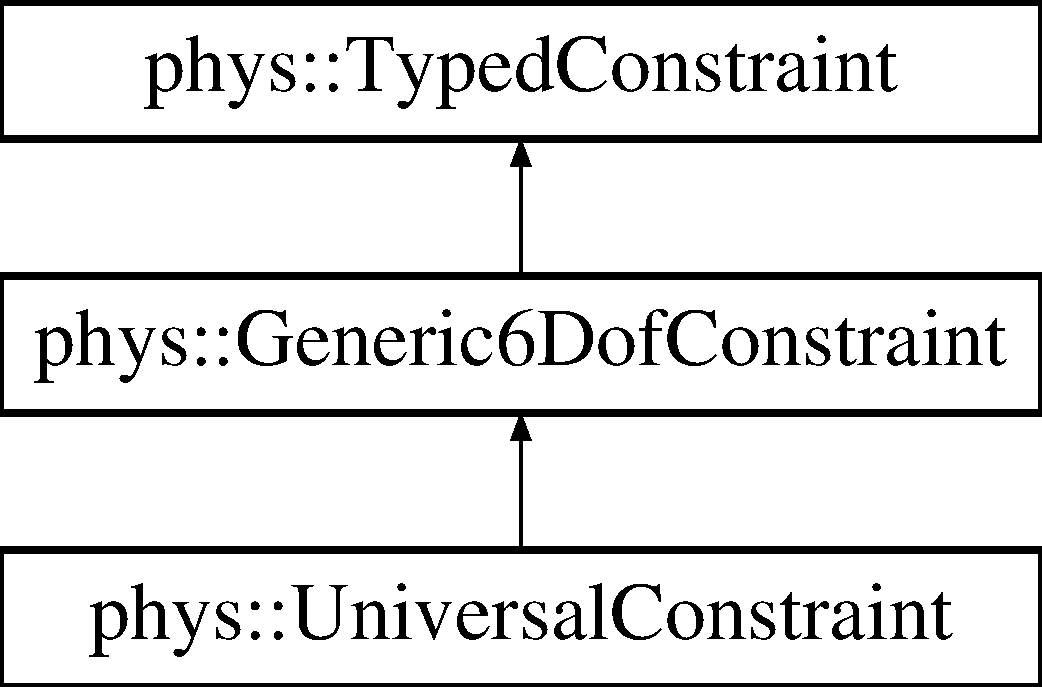
\includegraphics[height=3cm]{d0/d09/classphys_1_1UniversalConstraint}
\end{center}
\end{figure}
\subsection*{Public Member Functions}
\begin{DoxyCompactItemize}
\item 
\hypertarget{classphys_1_1UniversalConstraint_af08d5335171393e338b0617f99855701}{
{\bfseries UniversalConstraint} (\hyperlink{classphys_1_1ActorRigid}{ActorRigid} $\ast$\hyperlink{classphys_1_1TypedConstraint_a0fefb80c80d433bec9942b851b2f5a8a}{ActorA}, \hyperlink{classphys_1_1ActorRigid}{ActorRigid} $\ast$\hyperlink{classphys_1_1TypedConstraint_a04d2c49698d9a161e92112dd1efc1dcd}{ActorB}, \hyperlink{classphys_1_1Vector3}{Vector3} Anchor, \hyperlink{classphys_1_1Vector3}{Vector3} Axis1, \hyperlink{classphys_1_1Vector3}{Vector3} Axis2)}
\label{d0/d09/classphys_1_1UniversalConstraint_af08d5335171393e338b0617f99855701}

\item 
\hyperlink{classphys_1_1UniversalConstraint_af4d0828590b7fb242f601a171aa5db5f}{UniversalConstraint} (btUniversalConstraint $\ast$Constraint)
\begin{DoxyCompactList}\small\item\em Internal constructor. \item\end{DoxyCompactList}\item 
\hyperlink{classphys_1_1UniversalConstraint_aba3078f0f19a1a66c330d96f278e6fd8}{$\sim$UniversalConstraint} ()
\begin{DoxyCompactList}\small\item\em Class destructor. \item\end{DoxyCompactList}\item 
\hypertarget{classphys_1_1UniversalConstraint_a91e521aef75d4d32f91868ba31f486da}{
void {\bfseries SetUpperLimit} (\hyperlink{namespacephys_af7eb897198d265b8e868f45240230d5f}{Real} Ang1Max, \hyperlink{namespacephys_af7eb897198d265b8e868f45240230d5f}{Real} Ang2Max)}
\label{d0/d09/classphys_1_1UniversalConstraint_a91e521aef75d4d32f91868ba31f486da}

\item 
\hypertarget{classphys_1_1UniversalConstraint_a09b51abf3370f7834c9c1c2a326c57ca}{
void {\bfseries SetLowerLimit} (\hyperlink{namespacephys_af7eb897198d265b8e868f45240230d5f}{Real} Ang1Min, \hyperlink{namespacephys_af7eb897198d265b8e868f45240230d5f}{Real} Ang2Min)}
\label{d0/d09/classphys_1_1UniversalConstraint_a09b51abf3370f7834c9c1c2a326c57ca}

\end{DoxyCompactItemize}
\subsection*{Protected Attributes}
\begin{DoxyCompactItemize}
\item 
\hypertarget{classphys_1_1UniversalConstraint_ac05eed2dae4f659652d5a5ecd88bacf8}{
btUniversalConstraint $\ast$ \hyperlink{classphys_1_1UniversalConstraint_ac05eed2dae4f659652d5a5ecd88bacf8}{Universal}}
\label{d0/d09/classphys_1_1UniversalConstraint_ac05eed2dae4f659652d5a5ecd88bacf8}

\begin{DoxyCompactList}\small\item\em Bullet constraint that this class encapsulates. \item\end{DoxyCompactList}\end{DoxyCompactItemize}


\subsection{Detailed Description}


Definition at line 389 of file constraint.h.



\subsection{Constructor \& Destructor Documentation}
\hypertarget{classphys_1_1UniversalConstraint_af4d0828590b7fb242f601a171aa5db5f}{
\index{phys::UniversalConstraint@{phys::UniversalConstraint}!UniversalConstraint@{UniversalConstraint}}
\index{UniversalConstraint@{UniversalConstraint}!phys::UniversalConstraint@{phys::UniversalConstraint}}
\subsubsection[{UniversalConstraint}]{\setlength{\rightskip}{0pt plus 5cm}phys::UniversalConstraint::UniversalConstraint (btUniversalConstraint $\ast$ {\em Constraint})}}
\label{d0/d09/classphys_1_1UniversalConstraint_af4d0828590b7fb242f601a171aa5db5f}


Internal constructor. 

Constructs this class around a pre-\/built bullet constraint. This is an internal only constructor and shouldn't be called manually. 
\begin{DoxyParams}{Parameters}
\item[{\em Constraint}]The constraint to be constructed around. \end{DoxyParams}


Definition at line 745 of file constraint.cpp.

\hypertarget{classphys_1_1UniversalConstraint_aba3078f0f19a1a66c330d96f278e6fd8}{
\index{phys::UniversalConstraint@{phys::UniversalConstraint}!$\sim$UniversalConstraint@{$\sim$UniversalConstraint}}
\index{$\sim$UniversalConstraint@{$\sim$UniversalConstraint}!phys::UniversalConstraint@{phys::UniversalConstraint}}
\subsubsection[{$\sim$UniversalConstraint}]{\setlength{\rightskip}{0pt plus 5cm}phys::UniversalConstraint::$\sim$UniversalConstraint ()}}
\label{d0/d09/classphys_1_1UniversalConstraint_aba3078f0f19a1a66c330d96f278e6fd8}


Class destructor. 

The class destructor. 

Definition at line 752 of file constraint.cpp.



The documentation for this class was generated from the following files:\begin{DoxyCompactItemize}
\item 
constraint.h\item 
constraint.cpp\end{DoxyCompactItemize}

\hypertarget{classphys_1_1Vector2}{
\section{phys::Vector2 Class Reference}
\label{d0/d2c/classphys_1_1Vector2}\index{phys::Vector2@{phys::Vector2}}
}


This is used to represent a point on a 2 dimentional area, such as a screen.  




{\ttfamily \#include $<$vector2.h$>$}

\subsection*{Public Member Functions}
\begin{DoxyCompactItemize}
\item 
\hyperlink{classphys_1_1Vector2_a1e9c6000e5acd162a49836414a27bac7}{Vector2} ()
\begin{DoxyCompactList}\small\item\em Default Constructor. \item\end{DoxyCompactList}\item 
\hyperlink{classphys_1_1Vector2_ae8d3c95a5a60d12e706739cbadf01ffb}{Vector2} (\hyperlink{namespacephys_af7eb897198d265b8e868f45240230d5f}{Real} x, \hyperlink{namespacephys_af7eb897198d265b8e868f45240230d5f}{Real} y)
\begin{DoxyCompactList}\small\item\em Real value Constructor. \item\end{DoxyCompactList}\item 
\hyperlink{classphys_1_1Vector2_af3dbb91ef994e19b68c84e4e26eafac3}{Vector2} (Ogre::Vector2 Vec)
\begin{DoxyCompactList}\small\item\em Ogre Value Constructor. \item\end{DoxyCompactList}\item 
Ogre::Vector2 \hyperlink{classphys_1_1Vector2_adc6efedbdfdca596b719decc87ee2e4b}{GetOgreVector2} () const 
\begin{DoxyCompactList}\small\item\em Gets a Ogre vector2. \item\end{DoxyCompactList}\item 
void \hyperlink{classphys_1_1Vector2_af12824b786ce4b91443b5dbd700dfd58}{ExtractOgreVector2} (Ogre::Vector2 Ours)
\begin{DoxyCompactList}\small\item\em Copies an existing Ogre vector2. \item\end{DoxyCompactList}\item 
bool \hyperlink{classphys_1_1Vector2_a89874b6def8107146ca7079a2de49360}{operator==} (const \hyperlink{classphys_1_1Vector2}{phys::Vector2} \&Vec2)
\begin{DoxyCompactList}\small\item\em Equality Comparison Operator. \item\end{DoxyCompactList}\item 
bool \hyperlink{classphys_1_1Vector2_a074ca2a4d54925f745dbb9effd5c7e19}{operator!=} (const \hyperlink{classphys_1_1Vector2}{phys::Vector2} \&Vec2)
\begin{DoxyCompactList}\small\item\em Equality Comparison Operator. \item\end{DoxyCompactList}\item 
bool \hyperlink{classphys_1_1Vector2_a2fe433e9401748547b19cc5be891ed52}{operator==} (const Ogre::Vector2 \&Vec2)
\begin{DoxyCompactList}\small\item\em Equality Comparison Operator. \item\end{DoxyCompactList}\item 
bool \hyperlink{classphys_1_1Vector2_a186c1da597e1471a9ee5b07cc8bb9fb8}{operator!=} (const Ogre::Vector2 \&Vec2)
\begin{DoxyCompactList}\small\item\em Equality Comparison Operator. \item\end{DoxyCompactList}\item 
\hyperlink{classphys_1_1Vector2}{Vector2} \hyperlink{classphys_1_1Vector2_a59fa4aaadcccd04bf6de8fcd84b31c6d}{operator$\ast$} (const \hyperlink{namespacephys_af7eb897198d265b8e868f45240230d5f}{Real} \&scalar) const 
\begin{DoxyCompactList}\small\item\em Scaling by multiplication. \item\end{DoxyCompactList}\item 
\hyperlink{classphys_1_1Vector2}{Vector2} \hyperlink{classphys_1_1Vector2_a51f7d8ce03f7ab05137b277532edf93b}{operator/} (const \hyperlink{namespacephys_af7eb897198d265b8e868f45240230d5f}{Real} \&scalar) const 
\begin{DoxyCompactList}\small\item\em Scaling by Division. \item\end{DoxyCompactList}\item 
void \hyperlink{classphys_1_1Vector2_a0b1555274551eb9bdea20d762c446e99}{operator$\ast$=} (const \hyperlink{namespacephys_af7eb897198d265b8e868f45240230d5f}{Real} \&scalar)
\begin{DoxyCompactList}\small\item\em Scaling by multiplication. \item\end{DoxyCompactList}\item 
void \hyperlink{classphys_1_1Vector2_a27a0da5b4cfa49ea92dd16107692775b}{operator/=} (const \hyperlink{namespacephys_af7eb897198d265b8e868f45240230d5f}{Real} \&scalar)
\begin{DoxyCompactList}\small\item\em Scaling by Division. \item\end{DoxyCompactList}\item 
\hyperlink{classphys_1_1Vector2}{Vector2} \hyperlink{classphys_1_1Vector2_a62102e9d75364c6be43723867cec3df8}{operator+} (const \hyperlink{classphys_1_1Vector2}{Vector2} \&Vec2) const 
\begin{DoxyCompactList}\small\item\em Addition Operator. \item\end{DoxyCompactList}\item 
\hyperlink{classphys_1_1Vector2}{Vector2} \hyperlink{classphys_1_1Vector2_a0aef47f873ef5a78707dd850d7d59504}{operator-\/} (const \hyperlink{classphys_1_1Vector2}{Vector2} \&Vec2) const 
\begin{DoxyCompactList}\small\item\em Subraction Operator. \item\end{DoxyCompactList}\item 
\hyperlink{classphys_1_1Vector2}{Vector2} \hyperlink{classphys_1_1Vector2_a6a253bb2507b9254a102c0793bf0f215}{operator$\ast$} (const \hyperlink{classphys_1_1Vector2}{Vector2} \&Vec2) const 
\begin{DoxyCompactList}\small\item\em Multiplaction Operator. \item\end{DoxyCompactList}\item 
\hyperlink{classphys_1_1Vector2}{Vector2} \hyperlink{classphys_1_1Vector2_a3e4afe212ce1c739942aa8385c8f71e9}{operator/} (const \hyperlink{classphys_1_1Vector2}{Vector2} \&Vec2) const 
\begin{DoxyCompactList}\small\item\em Division Operator. \item\end{DoxyCompactList}\end{DoxyCompactItemize}
\subsection*{Public Attributes}
\begin{DoxyCompactItemize}
\item 
\hypertarget{classphys_1_1Vector2_a68e65741d34a298e420657180bf03d75}{
\hyperlink{namespacephys_af7eb897198d265b8e868f45240230d5f}{Real} \hyperlink{classphys_1_1Vector2_a68e65741d34a298e420657180bf03d75}{X}}
\label{d0/d2c/classphys_1_1Vector2_a68e65741d34a298e420657180bf03d75}

\begin{DoxyCompactList}\small\item\em Coordinate on the X vector. \item\end{DoxyCompactList}\item 
\hypertarget{classphys_1_1Vector2_ad1d77a1b2bf6c0040ecbd2b88b8a1ba4}{
\hyperlink{namespacephys_af7eb897198d265b8e868f45240230d5f}{Real} \hyperlink{classphys_1_1Vector2_ad1d77a1b2bf6c0040ecbd2b88b8a1ba4}{Y}}
\label{d0/d2c/classphys_1_1Vector2_ad1d77a1b2bf6c0040ecbd2b88b8a1ba4}

\begin{DoxyCompactList}\small\item\em Coordinate on the Y vector. \item\end{DoxyCompactList}\end{DoxyCompactItemize}


\subsection{Detailed Description}
This is used to represent a point on a 2 dimentional area, such as a screen. This contains an X and Y value used to represent coordinates. This also has a number of facilities to make converting to graphics subsystems as easy as possible. 

Definition at line 62 of file vector2.h.



\subsection{Constructor \& Destructor Documentation}
\hypertarget{classphys_1_1Vector2_a1e9c6000e5acd162a49836414a27bac7}{
\index{phys::Vector2@{phys::Vector2}!Vector2@{Vector2}}
\index{Vector2@{Vector2}!phys::Vector2@{phys::Vector2}}
\subsubsection[{Vector2}]{\setlength{\rightskip}{0pt plus 5cm}phys::Vector2::Vector2 (
\begin{DoxyParamCaption}
{}
\end{DoxyParamCaption}
)}}
\label{d0/d2c/classphys_1_1Vector2_a1e9c6000e5acd162a49836414a27bac7}


Default Constructor. 

Basic all zero initialization constructor. 

Definition at line 48 of file vector2.cpp.

\hypertarget{classphys_1_1Vector2_ae8d3c95a5a60d12e706739cbadf01ffb}{
\index{phys::Vector2@{phys::Vector2}!Vector2@{Vector2}}
\index{Vector2@{Vector2}!phys::Vector2@{phys::Vector2}}
\subsubsection[{Vector2}]{\setlength{\rightskip}{0pt plus 5cm}phys::Vector2::Vector2 (
\begin{DoxyParamCaption}
\item[{{\bf Real}}]{ x, }
\item[{{\bf Real}}]{ y}
\end{DoxyParamCaption}
)}}
\label{d0/d2c/classphys_1_1Vector2_ae8d3c95a5a60d12e706739cbadf01ffb}


Real value Constructor. 

Constructor that sets both vectors. 
\begin{DoxyParams}{Parameters}
\item[{\em x}]Coordinate on the X vector. \item[{\em y}]Coordinate on the Y vector. \end{DoxyParams}


Definition at line 54 of file vector2.cpp.

\hypertarget{classphys_1_1Vector2_af3dbb91ef994e19b68c84e4e26eafac3}{
\index{phys::Vector2@{phys::Vector2}!Vector2@{Vector2}}
\index{Vector2@{Vector2}!phys::Vector2@{phys::Vector2}}
\subsubsection[{Vector2}]{\setlength{\rightskip}{0pt plus 5cm}phys::Vector2::Vector2 (
\begin{DoxyParamCaption}
\item[{Ogre::Vector2}]{ Vec}
\end{DoxyParamCaption}
)}}
\label{d0/d2c/classphys_1_1Vector2_af3dbb91ef994e19b68c84e4e26eafac3}


Ogre Value Constructor. 

Constructor that sets all values to match the Ogre vector. 
\begin{DoxyParams}{Parameters}
\item[{\em Vec}]The vector to be copied to make this vector. \end{DoxyParams}


Definition at line 60 of file vector2.cpp.



\subsection{Member Function Documentation}
\hypertarget{classphys_1_1Vector2_af12824b786ce4b91443b5dbd700dfd58}{
\index{phys::Vector2@{phys::Vector2}!ExtractOgreVector2@{ExtractOgreVector2}}
\index{ExtractOgreVector2@{ExtractOgreVector2}!phys::Vector2@{phys::Vector2}}
\subsubsection[{ExtractOgreVector2}]{\setlength{\rightskip}{0pt plus 5cm}void phys::Vector2::ExtractOgreVector2 (
\begin{DoxyParamCaption}
\item[{Ogre::Vector2}]{ Ours}
\end{DoxyParamCaption}
)}}
\label{d0/d2c/classphys_1_1Vector2_af12824b786ce4b91443b5dbd700dfd58}


Copies an existing Ogre vector2. 

This function will copy the values stored in an existing Ogre vector2 and set the values of this class to be the same. 
\begin{DoxyParams}{Parameters}
\item[{\em Ours}]The vector2 to be extracted. \end{DoxyParams}


Definition at line 73 of file vector2.cpp.

\hypertarget{classphys_1_1Vector2_adc6efedbdfdca596b719decc87ee2e4b}{
\index{phys::Vector2@{phys::Vector2}!GetOgreVector2@{GetOgreVector2}}
\index{GetOgreVector2@{GetOgreVector2}!phys::Vector2@{phys::Vector2}}
\subsubsection[{GetOgreVector2}]{\setlength{\rightskip}{0pt plus 5cm}Ogre::Vector2 phys::Vector2::GetOgreVector2 (
\begin{DoxyParamCaption}
{}
\end{DoxyParamCaption}
) const}}
\label{d0/d2c/classphys_1_1Vector2_adc6efedbdfdca596b719decc87ee2e4b}


Gets a Ogre vector2. 

Creates a Ogre vector2 with values equal to this class and returns it. 

Definition at line 65 of file vector2.cpp.

\hypertarget{classphys_1_1Vector2_a074ca2a4d54925f745dbb9effd5c7e19}{
\index{phys::Vector2@{phys::Vector2}!operator!=@{operator!=}}
\index{operator!=@{operator!=}!phys::Vector2@{phys::Vector2}}
\subsubsection[{operator!=}]{\setlength{\rightskip}{0pt plus 5cm}bool phys::Vector2::operator!= (
\begin{DoxyParamCaption}
\item[{const {\bf phys::Vector2} \&}]{ Vec2}
\end{DoxyParamCaption}
)}}
\label{d0/d2c/classphys_1_1Vector2_a074ca2a4d54925f745dbb9effd5c7e19}


Equality Comparison Operator. 

Returns true if X!=X or Y!=Y. If any of those do not match this returns false. 
\begin{DoxyParams}{Parameters}
\item[{\em Vec2}]This is the other \hyperlink{classphys_1_1Vector2}{phys::Vector2}. \end{DoxyParams}


Definition at line 89 of file vector2.cpp.

\hypertarget{classphys_1_1Vector2_a186c1da597e1471a9ee5b07cc8bb9fb8}{
\index{phys::Vector2@{phys::Vector2}!operator!=@{operator!=}}
\index{operator!=@{operator!=}!phys::Vector2@{phys::Vector2}}
\subsubsection[{operator!=}]{\setlength{\rightskip}{0pt plus 5cm}bool phys::Vector2::operator!= (
\begin{DoxyParamCaption}
\item[{const Ogre::Vector2 \&}]{ Vec2}
\end{DoxyParamCaption}
)}}
\label{d0/d2c/classphys_1_1Vector2_a186c1da597e1471a9ee5b07cc8bb9fb8}


Equality Comparison Operator. 

Returns true if X!=X or Y!=Y. If any of those do not match this returns false. 
\begin{DoxyParams}{Parameters}
\item[{\em Vec2}]This is the other Ogre::Vector2. \end{DoxyParams}


Definition at line 103 of file vector2.cpp.

\hypertarget{classphys_1_1Vector2_a6a253bb2507b9254a102c0793bf0f215}{
\index{phys::Vector2@{phys::Vector2}!operator$\ast$@{operator$\ast$}}
\index{operator$\ast$@{operator$\ast$}!phys::Vector2@{phys::Vector2}}
\subsubsection[{operator$\ast$}]{\setlength{\rightskip}{0pt plus 5cm}{\bf Vector2} phys::Vector2::operator$\ast$ (
\begin{DoxyParamCaption}
\item[{const {\bf Vector2} \&}]{ Vec2}
\end{DoxyParamCaption}
) const}}
\label{d0/d2c/classphys_1_1Vector2_a6a253bb2507b9254a102c0793bf0f215}


Multiplaction Operator. 

Allows for multiplaction from a \hyperlink{classphys_1_1Vector2}{phys::Vector2} 
\begin{DoxyParams}{Parameters}
\item[{\em Vec2}]This is the other \hyperlink{classphys_1_1Vector2}{phys::Vector2} \end{DoxyParams}


Definition at line 161 of file vector2.cpp.

\hypertarget{classphys_1_1Vector2_a59fa4aaadcccd04bf6de8fcd84b31c6d}{
\index{phys::Vector2@{phys::Vector2}!operator$\ast$@{operator$\ast$}}
\index{operator$\ast$@{operator$\ast$}!phys::Vector2@{phys::Vector2}}
\subsubsection[{operator$\ast$}]{\setlength{\rightskip}{0pt plus 5cm}{\bf Vector2} phys::Vector2::operator$\ast$ (
\begin{DoxyParamCaption}
\item[{const {\bf Real} \&}]{ scalar}
\end{DoxyParamCaption}
) const}}
\label{d0/d2c/classphys_1_1Vector2_a59fa4aaadcccd04bf6de8fcd84b31c6d}


Scaling by multiplication. 

This Multiplies X, Y and Z by scalar \begin{DoxyReturn}{Returns}
This returns a \hyperlink{classphys_1_1Vector2}{Vector2} that has been scaled 
\end{DoxyReturn}

\begin{DoxyParams}{Parameters}
\item[{\em scalar}]This is the amount to scale the \hyperlink{classphys_1_1Vector2}{Vector2} by \end{DoxyParams}


Definition at line 112 of file vector2.cpp.

\hypertarget{classphys_1_1Vector2_a0b1555274551eb9bdea20d762c446e99}{
\index{phys::Vector2@{phys::Vector2}!operator$\ast$=@{operator$\ast$=}}
\index{operator$\ast$=@{operator$\ast$=}!phys::Vector2@{phys::Vector2}}
\subsubsection[{operator$\ast$=}]{\setlength{\rightskip}{0pt plus 5cm}void phys::Vector2::operator$\ast$= (
\begin{DoxyParamCaption}
\item[{const {\bf Real} \&}]{ scalar}
\end{DoxyParamCaption}
)}}
\label{d0/d2c/classphys_1_1Vector2_a0b1555274551eb9bdea20d762c446e99}


Scaling by multiplication. 

This Multiplies X, Y and Z by scalar and stores the changes in this \hyperlink{classphys_1_1Vector2}{Vector2}. 
\begin{DoxyParams}{Parameters}
\item[{\em scalar}]This is the amount to scale the \hyperlink{classphys_1_1Vector2}{Vector2} by. \end{DoxyParams}


Definition at line 130 of file vector2.cpp.

\hypertarget{classphys_1_1Vector2_a62102e9d75364c6be43723867cec3df8}{
\index{phys::Vector2@{phys::Vector2}!operator+@{operator+}}
\index{operator+@{operator+}!phys::Vector2@{phys::Vector2}}
\subsubsection[{operator+}]{\setlength{\rightskip}{0pt plus 5cm}{\bf Vector2} phys::Vector2::operator+ (
\begin{DoxyParamCaption}
\item[{const {\bf Vector2} \&}]{ Vec2}
\end{DoxyParamCaption}
) const}}
\label{d0/d2c/classphys_1_1Vector2_a62102e9d75364c6be43723867cec3df8}


Addition Operator. 

Allows for addition from a \hyperlink{classphys_1_1Vector2}{phys::Vector2} 
\begin{DoxyParams}{Parameters}
\item[{\em Vec2}]This is the other \hyperlink{classphys_1_1Vector2}{phys::Vector2} \end{DoxyParams}


Definition at line 145 of file vector2.cpp.

\hypertarget{classphys_1_1Vector2_a0aef47f873ef5a78707dd850d7d59504}{
\index{phys::Vector2@{phys::Vector2}!operator-\/@{operator-\/}}
\index{operator-\/@{operator-\/}!phys::Vector2@{phys::Vector2}}
\subsubsection[{operator-\/}]{\setlength{\rightskip}{0pt plus 5cm}{\bf Vector2} phys::Vector2::operator-\/ (
\begin{DoxyParamCaption}
\item[{const {\bf Vector2} \&}]{ Vec2}
\end{DoxyParamCaption}
) const}}
\label{d0/d2c/classphys_1_1Vector2_a0aef47f873ef5a78707dd850d7d59504}


Subraction Operator. 

Allows for subtraction from a \hyperlink{classphys_1_1Vector2}{phys::Vector2} 
\begin{DoxyParams}{Parameters}
\item[{\em Vec2}]This is the other \hyperlink{classphys_1_1Vector2}{phys::Vector2} \end{DoxyParams}


Definition at line 153 of file vector2.cpp.

\hypertarget{classphys_1_1Vector2_a51f7d8ce03f7ab05137b277532edf93b}{
\index{phys::Vector2@{phys::Vector2}!operator/@{operator/}}
\index{operator/@{operator/}!phys::Vector2@{phys::Vector2}}
\subsubsection[{operator/}]{\setlength{\rightskip}{0pt plus 5cm}{\bf Vector2} phys::Vector2::operator/ (
\begin{DoxyParamCaption}
\item[{const {\bf Real} \&}]{ scalar}
\end{DoxyParamCaption}
) const}}
\label{d0/d2c/classphys_1_1Vector2_a51f7d8ce03f7ab05137b277532edf93b}


Scaling by Division. 

This Diisionn X, Y and Z by scalar \begin{DoxyReturn}{Returns}
This returns a \hyperlink{classphys_1_1Vector2}{Vector2} that has been scaled 
\end{DoxyReturn}

\begin{DoxyParams}{Parameters}
\item[{\em scalar}]This is the amount to scale the \hyperlink{classphys_1_1Vector2}{Vector2} by \end{DoxyParams}


Definition at line 120 of file vector2.cpp.

\hypertarget{classphys_1_1Vector2_a3e4afe212ce1c739942aa8385c8f71e9}{
\index{phys::Vector2@{phys::Vector2}!operator/@{operator/}}
\index{operator/@{operator/}!phys::Vector2@{phys::Vector2}}
\subsubsection[{operator/}]{\setlength{\rightskip}{0pt plus 5cm}{\bf Vector2} phys::Vector2::operator/ (
\begin{DoxyParamCaption}
\item[{const {\bf Vector2} \&}]{ Vec2}
\end{DoxyParamCaption}
) const}}
\label{d0/d2c/classphys_1_1Vector2_a3e4afe212ce1c739942aa8385c8f71e9}


Division Operator. 

Allows for division from a \hyperlink{classphys_1_1Vector2}{phys::Vector2} 
\begin{DoxyParams}{Parameters}
\item[{\em Vec2}]This is the other \hyperlink{classphys_1_1Vector2}{phys::Vector2} \end{DoxyParams}


Definition at line 169 of file vector2.cpp.

\hypertarget{classphys_1_1Vector2_a27a0da5b4cfa49ea92dd16107692775b}{
\index{phys::Vector2@{phys::Vector2}!operator/=@{operator/=}}
\index{operator/=@{operator/=}!phys::Vector2@{phys::Vector2}}
\subsubsection[{operator/=}]{\setlength{\rightskip}{0pt plus 5cm}void phys::Vector2::operator/= (
\begin{DoxyParamCaption}
\item[{const {\bf Real} \&}]{ scalar}
\end{DoxyParamCaption}
)}}
\label{d0/d2c/classphys_1_1Vector2_a27a0da5b4cfa49ea92dd16107692775b}


Scaling by Division. 

This Division X, Y and Z by scalar and and stores the changes in this \hyperlink{classphys_1_1Vector2}{Vector2}. 
\begin{DoxyParams}{Parameters}
\item[{\em scalar}]This is the amount to scale the \hyperlink{classphys_1_1Vector2}{Vector2} by \end{DoxyParams}


Definition at line 136 of file vector2.cpp.

\hypertarget{classphys_1_1Vector2_a2fe433e9401748547b19cc5be891ed52}{
\index{phys::Vector2@{phys::Vector2}!operator==@{operator==}}
\index{operator==@{operator==}!phys::Vector2@{phys::Vector2}}
\subsubsection[{operator==}]{\setlength{\rightskip}{0pt plus 5cm}bool phys::Vector2::operator== (
\begin{DoxyParamCaption}
\item[{const Ogre::Vector2 \&}]{ Vec2}
\end{DoxyParamCaption}
)}}
\label{d0/d2c/classphys_1_1Vector2_a2fe433e9401748547b19cc5be891ed52}


Equality Comparison Operator. 

Returns true if X==X and Y==Y. If any of those do not match this returns false. 
\begin{DoxyParams}{Parameters}
\item[{\em Vec2}]This is the other Ogre::Vector2. \end{DoxyParams}


Definition at line 96 of file vector2.cpp.

\hypertarget{classphys_1_1Vector2_a89874b6def8107146ca7079a2de49360}{
\index{phys::Vector2@{phys::Vector2}!operator==@{operator==}}
\index{operator==@{operator==}!phys::Vector2@{phys::Vector2}}
\subsubsection[{operator==}]{\setlength{\rightskip}{0pt plus 5cm}bool phys::Vector2::operator== (
\begin{DoxyParamCaption}
\item[{const {\bf phys::Vector2} \&}]{ Vec2}
\end{DoxyParamCaption}
)}}
\label{d0/d2c/classphys_1_1Vector2_a89874b6def8107146ca7079a2de49360}


Equality Comparison Operator. 

Returns true if X==X and Y==Y. If any of those do not match this returns false. 
\begin{DoxyParams}{Parameters}
\item[{\em Vec2}]This is the other \hyperlink{classphys_1_1Vector2}{phys::Vector2}. \end{DoxyParams}


Definition at line 82 of file vector2.cpp.



The documentation for this class was generated from the following files:\begin{DoxyCompactItemize}
\item 
vector2.h\item 
vector2.cpp\end{DoxyCompactItemize}

\hypertarget{classphys_1_1Vector3}{
\section{phys::Vector3 Class Reference}
\label{d5/d6a/classphys_1_1Vector3}\index{phys::Vector3@{phys::Vector3}}
}


This is used to represent a point in space, or a vector through space.  




{\ttfamily \#include $<$vector3.h$>$}

\subsection*{Public Member Functions}
\begin{DoxyCompactItemize}
\item 
\hyperlink{classphys_1_1Vector3_af328c400a03fdb8d2a99fd58382d61cb}{Vector3} ()
\begin{DoxyCompactList}\small\item\em Default Constructor. \item\end{DoxyCompactList}\item 
\hyperlink{classphys_1_1Vector3_af1d323b44d7b6ee3d0a79a196d9967da}{Vector3} (\hyperlink{namespacephys_af7eb897198d265b8e868f45240230d5f}{Real} \hyperlink{classphys_1_1Vector3_a23660f9d1e21a25c53aa06aa737bb56b}{X}, \hyperlink{namespacephys_af7eb897198d265b8e868f45240230d5f}{Real} \hyperlink{classphys_1_1Vector3_a6c9bc2ab0995d5056dba8272c650e58e}{Y}, \hyperlink{namespacephys_af7eb897198d265b8e868f45240230d5f}{Real} \hyperlink{classphys_1_1Vector3_a53c84fa4b38fb9c4a4d822b04c200b13}{Z})
\begin{DoxyCompactList}\small\item\em Real value Constructor. \item\end{DoxyCompactList}\item 
\hyperlink{classphys_1_1Vector3_ad19c9ae00070b3aad5799e1f8c00bd34}{Vector3} (Ogre::Vector3 Vec)
\begin{DoxyCompactList}\small\item\em Ogre Value Constructor. \item\end{DoxyCompactList}\item 
\hyperlink{classphys_1_1Vector3_a8ff2e969410341eaf328ab76fb3099ed}{Vector3} (btVector3 Vec)
\begin{DoxyCompactList}\small\item\em Bullet Value Constructor. \item\end{DoxyCompactList}\item 
\hyperlink{classphys_1_1Vector3_a0ed3fe0518fc5e29544234bd41091401}{Vector3} (cAudio::cVector3 Vec)
\begin{DoxyCompactList}\small\item\em cAudio Value Constructor. \item\end{DoxyCompactList}\item 
\hyperlink{classphys_1_1Vector3}{Vector3} \& \hyperlink{classphys_1_1Vector3_a81a755b7fd93ad523c63befe773b7359}{operator=} (const btVector3 \&bt3)
\begin{DoxyCompactList}\small\item\em Assignment operator to convert from Bullet Vectors. \item\end{DoxyCompactList}\item 
\hyperlink{classphys_1_1Vector3}{Vector3} \& \hyperlink{classphys_1_1Vector3_a4c9602b683617d91a68ec1e885522b8b}{operator=} (const Ogre::Vector3 \&OVec3)
\begin{DoxyCompactList}\small\item\em Assignment operator to convert from Ogre Vectors. \item\end{DoxyCompactList}\item 
bool \hyperlink{classphys_1_1Vector3_a90dadb1a5cd2c5814e54c11c33f286c1}{operator==} (const \hyperlink{classphys_1_1Vector3}{phys::Vector3} \&Vec2)
\begin{DoxyCompactList}\small\item\em Equality Comparison Operator. \item\end{DoxyCompactList}\item 
bool \hyperlink{classphys_1_1Vector3_a1146d1b1b0f3d8809edfbd24e79b724a}{operator==} (const btVector3 \&Vec2)
\begin{DoxyCompactList}\small\item\em Equality Comparison Operator. \item\end{DoxyCompactList}\item 
bool \hyperlink{classphys_1_1Vector3_aef82f53ef74363d7b662cbd1d3c204db}{operator==} (const Ogre::Vector3 \&Vec2)
\begin{DoxyCompactList}\small\item\em Equality Comparison Operator. \item\end{DoxyCompactList}\item 
\hyperlink{classphys_1_1Vector3}{Vector3} \hyperlink{classphys_1_1Vector3_afb86ac7edd78353ec3d11d9f2efdf0cb}{operator-\/} ()
\begin{DoxyCompactList}\small\item\em Additive Inverse Operator. \item\end{DoxyCompactList}\item 
\hyperlink{classphys_1_1Vector3}{Vector3} \hyperlink{classphys_1_1Vector3_ab9b40eb9eb73d806434550604e048faa}{operator$\ast$} (const \hyperlink{namespacephys_af7eb897198d265b8e868f45240230d5f}{Real} \&scalar) const 
\begin{DoxyCompactList}\small\item\em Scaling by multiplication. \item\end{DoxyCompactList}\item 
\hyperlink{classphys_1_1Vector3}{Vector3} \hyperlink{classphys_1_1Vector3_a4bb5377ad78c299b40a8bc9fb66a902f}{operator/} (const \hyperlink{namespacephys_af7eb897198d265b8e868f45240230d5f}{Real} \&scalar) const 
\begin{DoxyCompactList}\small\item\em Scaling by Division. \item\end{DoxyCompactList}\item 
void \hyperlink{classphys_1_1Vector3_ae04a2cdca40ac24180d6fb62babb34d7}{operator$\ast$=} (const \hyperlink{namespacephys_af7eb897198d265b8e868f45240230d5f}{Real} \&scalar)
\begin{DoxyCompactList}\small\item\em Scaling by multiplication. \item\end{DoxyCompactList}\item 
void \hyperlink{classphys_1_1Vector3_ae16bc8ff2f9897b52c36655a8ba8a1be}{operator/=} (const \hyperlink{namespacephys_af7eb897198d265b8e868f45240230d5f}{Real} \&scalar)
\begin{DoxyCompactList}\small\item\em Scaling by Division. \item\end{DoxyCompactList}\item 
\hyperlink{classphys_1_1Vector3}{Vector3} \hyperlink{classphys_1_1Vector3_ab9799d4796f3750d44f591986d78e436}{operator+} (const \hyperlink{classphys_1_1Vector3}{Vector3} \&Vec2) const 
\begin{DoxyCompactList}\small\item\em Addition Operator. \item\end{DoxyCompactList}\item 
\hyperlink{classphys_1_1Vector3}{Vector3} \hyperlink{classphys_1_1Vector3_aed320f9ac1374c0955a20aef50c05751}{operator-\/} (const \hyperlink{classphys_1_1Vector3}{Vector3} \&Vec2) const 
\begin{DoxyCompactList}\small\item\em Subraction Operator. \item\end{DoxyCompactList}\item 
\hyperlink{classphys_1_1Vector3}{Vector3} \hyperlink{classphys_1_1Vector3_aa148f18ae4cae10a4aae4170351d7c11}{operator$\ast$} (const \hyperlink{classphys_1_1Vector3}{Vector3} \&Vec2) const 
\begin{DoxyCompactList}\small\item\em Multiplaction Operator. \item\end{DoxyCompactList}\item 
\hyperlink{classphys_1_1Vector3}{Vector3} \hyperlink{classphys_1_1Vector3_af8db5066a9509a5d1b7d568ef576dc6e}{operator/} (const \hyperlink{classphys_1_1Vector3}{Vector3} \&Vec2) const 
\begin{DoxyCompactList}\small\item\em Division Operator. \item\end{DoxyCompactList}\item 
\hyperlink{classphys_1_1Vector3}{Vector3} \hyperlink{classphys_1_1Vector3_a70c99d125274635b07b0fe90bcc15a8c}{operator+} (const btVector3 \&Vec2)
\begin{DoxyCompactList}\small\item\em Bullet Addition Operator. \item\end{DoxyCompactList}\item 
\hyperlink{classphys_1_1Vector3}{Vector3} \hyperlink{classphys_1_1Vector3_ab7ec10d90e35c2b153a2f002f12518ce}{operator-\/} (const btVector3 \&Vec2)
\begin{DoxyCompactList}\small\item\em Bullet Subtraction Operator. \item\end{DoxyCompactList}\item 
\hyperlink{classphys_1_1Vector3}{Vector3} \hyperlink{classphys_1_1Vector3_a59f8b8d5c15f4b047100480ad26ba092}{operator$\ast$} (const btVector3 \&Vec2)
\begin{DoxyCompactList}\small\item\em Bullet Multiplication Operator. \item\end{DoxyCompactList}\item 
\hyperlink{classphys_1_1Vector3}{Vector3} \hyperlink{classphys_1_1Vector3_a945287bb9448b2353c90e16c6cfed876}{operator/} (const btVector3 \&Vec2)
\begin{DoxyCompactList}\small\item\em Bullet Division Operator. \item\end{DoxyCompactList}\item 
\hyperlink{classphys_1_1Vector3}{Vector3} \hyperlink{classphys_1_1Vector3_a14ca2ae8bbe9ebefd298486b2a2ba5c9}{operator+} (const Ogre::Vector3 \&Vec2)
\begin{DoxyCompactList}\small\item\em Ogre Addition Operator. \item\end{DoxyCompactList}\item 
\hyperlink{classphys_1_1Vector3}{Vector3} \hyperlink{classphys_1_1Vector3_a54d5fc20ae502ac1443ddbb6cf1fbf1f}{operator-\/} (const Ogre::Vector3 \&Vec2)
\begin{DoxyCompactList}\small\item\em Bullet Subtraction Operator. \item\end{DoxyCompactList}\item 
\hyperlink{classphys_1_1Vector3}{Vector3} \hyperlink{classphys_1_1Vector3_a34014be39219a1ad3d4808b9614ac80d}{operator$\ast$} (const Ogre::Vector3 \&Vec2)
\begin{DoxyCompactList}\small\item\em Bullet Multiplication Operator. \item\end{DoxyCompactList}\item 
\hyperlink{classphys_1_1Vector3}{Vector3} \hyperlink{classphys_1_1Vector3_a4f9f3240dab2277e8a9b80f6c7235e5b}{operator/} (const Ogre::Vector3 \&Vec2)
\begin{DoxyCompactList}\small\item\em Bullet Division Operator. \item\end{DoxyCompactList}\item 
\hyperlink{classphys_1_1Vector3}{Vector3} \hyperlink{classphys_1_1Vector3_ae98b11238914cd77a729053798ebf339}{CrossProduct} (const \hyperlink{classphys_1_1Vector3}{Vector3} \&rkVector) const 
\begin{DoxyCompactList}\small\item\em This is used to calculate the crossproduct of this and another vector. \item\end{DoxyCompactList}\item 
\hyperlink{namespacephys_af7eb897198d265b8e868f45240230d5f}{Real} \hyperlink{classphys_1_1Vector3_ac30ef9729b1a4e6001f5f5219a88176d}{dotProduct} (const \hyperlink{classphys_1_1Vector3}{Vector3} \&vec) const 
\begin{DoxyCompactList}\small\item\em This is used to calculate the dotproduct of this and another vector. \item\end{DoxyCompactList}\item 
void \hyperlink{classphys_1_1Vector3_ae39fe0545df88148bcd668b3bd2a4388}{Normalize} ()
\begin{DoxyCompactList}\small\item\em This will change this point into it's own normal relative to the origin. \item\end{DoxyCompactList}\item 
\hyperlink{classphys_1_1Vector3}{Vector3} \hyperlink{classphys_1_1Vector3_a81e11f45378758391c97ec55b519951c}{GetNormal} () const 
\begin{DoxyCompactList}\small\item\em This returns the normal for this relative to the origin. \item\end{DoxyCompactList}\item 
\hyperlink{classphys_1_1Vector3}{Vector3} \hyperlink{classphys_1_1Vector3_a63cd464cdd9ba976ac112fdf8bb620be}{GetDirection} (const \hyperlink{classphys_1_1Vector3}{Vector3} \&Destination) const 
\begin{DoxyCompactList}\small\item\em This will get the direction between two points. \item\end{DoxyCompactList}\item 
void \hyperlink{classphys_1_1Vector3_a30af9c8ae51596fa00fa7f350f9668f5}{Inverse} ()
\begin{DoxyCompactList}\small\item\em This will inverse the reals in the vector. \item\end{DoxyCompactList}\item 
btVector3 \hyperlink{classphys_1_1Vector3_adf4129007ee41f5a03e97502f2df9c41}{GetBulletVector3} () const 
\begin{DoxyCompactList}\small\item\em Gets a Bullet vector3. \item\end{DoxyCompactList}\item 
void \hyperlink{classphys_1_1Vector3_a24ae86b068340be6727877f8c6c1a313}{ExtractBulletVector3} (btVector3 temp)
\begin{DoxyCompactList}\small\item\em Copies an existing Bullet vector3. \item\end{DoxyCompactList}\item 
Ogre::Vector3 \hyperlink{classphys_1_1Vector3_a17265d86a74139398d310b56ba7e89b8}{GetOgreVector3} () const 
\begin{DoxyCompactList}\small\item\em Gets a Ogre vector3. \item\end{DoxyCompactList}\item 
void \hyperlink{classphys_1_1Vector3_a09a31cb8fe491f61e0cc10d21705a0df}{ExtractOgreVector3} (Ogre::Vector3 temp)
\begin{DoxyCompactList}\small\item\em Copies an existing Ogre vector3. \item\end{DoxyCompactList}\item 
cAudio::cVector3 \hyperlink{classphys_1_1Vector3_a58b1ac39dfee4c360c16944a7e7f657d}{GetcAudioVector3} () const 
\begin{DoxyCompactList}\small\item\em Gets a cAudio vector3. \item\end{DoxyCompactList}\item 
void \hyperlink{classphys_1_1Vector3_aa12021e9cdc092c8628ced1c5910c04c}{ExtractcAudioVector3} (cAudio::cVector3 temp)
\begin{DoxyCompactList}\small\item\em Copies an existing cAudio vector3. \item\end{DoxyCompactList}\item 
\hyperlink{namespacephys_af7eb897198d265b8e868f45240230d5f}{Real} \hyperlink{classphys_1_1Vector3_af59a586331fe9497056b7e0f207658a3}{Distance} (const \hyperlink{classphys_1_1Vector3}{Vector3} \&OtherVec) const 
\begin{DoxyCompactList}\small\item\em This return the distance between this point and another. \item\end{DoxyCompactList}\end{DoxyCompactItemize}
\subsection*{Public Attributes}
\begin{DoxyCompactItemize}
\item 
\hypertarget{classphys_1_1Vector3_a23660f9d1e21a25c53aa06aa737bb56b}{
\hyperlink{namespacephys_af7eb897198d265b8e868f45240230d5f}{Real} \hyperlink{classphys_1_1Vector3_a23660f9d1e21a25c53aa06aa737bb56b}{X}}
\label{d5/d6a/classphys_1_1Vector3_a23660f9d1e21a25c53aa06aa737bb56b}

\begin{DoxyCompactList}\small\item\em Coordinate on the X vector. \item\end{DoxyCompactList}\item 
\hypertarget{classphys_1_1Vector3_a6c9bc2ab0995d5056dba8272c650e58e}{
\hyperlink{namespacephys_af7eb897198d265b8e868f45240230d5f}{Real} \hyperlink{classphys_1_1Vector3_a6c9bc2ab0995d5056dba8272c650e58e}{Y}}
\label{d5/d6a/classphys_1_1Vector3_a6c9bc2ab0995d5056dba8272c650e58e}

\begin{DoxyCompactList}\small\item\em Coordinate on the Y vector. \item\end{DoxyCompactList}\item 
\hypertarget{classphys_1_1Vector3_a53c84fa4b38fb9c4a4d822b04c200b13}{
\hyperlink{namespacephys_af7eb897198d265b8e868f45240230d5f}{Real} \hyperlink{classphys_1_1Vector3_a53c84fa4b38fb9c4a4d822b04c200b13}{Z}}
\label{d5/d6a/classphys_1_1Vector3_a53c84fa4b38fb9c4a4d822b04c200b13}

\begin{DoxyCompactList}\small\item\em Coordinate on the Z vector. \item\end{DoxyCompactList}\end{DoxyCompactItemize}


\subsection{Detailed Description}
This is used to represent a point in space, or a vector through space. This contains an X, Y and a Z value used to represent coordinates. This also has a number of facilities to make converting from Physics subsystem vectors or graphics subsystems as easy as possible 

Definition at line 67 of file vector3.h.



\subsection{Constructor \& Destructor Documentation}
\hypertarget{classphys_1_1Vector3_af328c400a03fdb8d2a99fd58382d61cb}{
\index{phys::Vector3@{phys::Vector3}!Vector3@{Vector3}}
\index{Vector3@{Vector3}!phys::Vector3@{phys::Vector3}}
\subsubsection[{Vector3}]{\setlength{\rightskip}{0pt plus 5cm}phys::Vector3::Vector3 (
\begin{DoxyParamCaption}
{}
\end{DoxyParamCaption}
)}}
\label{d5/d6a/classphys_1_1Vector3_af328c400a03fdb8d2a99fd58382d61cb}


Default Constructor. 

Basic all zero initialization constructor. 

Definition at line 56 of file vector3.cpp.

\hypertarget{classphys_1_1Vector3_af1d323b44d7b6ee3d0a79a196d9967da}{
\index{phys::Vector3@{phys::Vector3}!Vector3@{Vector3}}
\index{Vector3@{Vector3}!phys::Vector3@{phys::Vector3}}
\subsubsection[{Vector3}]{\setlength{\rightskip}{0pt plus 5cm}phys::Vector3::Vector3 (
\begin{DoxyParamCaption}
\item[{{\bf Real}}]{ X, }
\item[{{\bf Real}}]{ Y, }
\item[{{\bf Real}}]{ Z}
\end{DoxyParamCaption}
)}}
\label{d5/d6a/classphys_1_1Vector3_af1d323b44d7b6ee3d0a79a196d9967da}


Real value Constructor. 

Constructor that sets all three vectors. 
\begin{DoxyParams}{Parameters}
\item[{\em X}]Coordinate on the X vector. \item[{\em Y}]Coordinate on the Y vector. \item[{\em Z}]Coordinate on the Z vector. \end{DoxyParams}


Definition at line 63 of file vector3.cpp.

\hypertarget{classphys_1_1Vector3_ad19c9ae00070b3aad5799e1f8c00bd34}{
\index{phys::Vector3@{phys::Vector3}!Vector3@{Vector3}}
\index{Vector3@{Vector3}!phys::Vector3@{phys::Vector3}}
\subsubsection[{Vector3}]{\setlength{\rightskip}{0pt plus 5cm}phys::Vector3::Vector3 (
\begin{DoxyParamCaption}
\item[{Ogre::Vector3}]{ Vec}
\end{DoxyParamCaption}
)\hspace{0.3cm}{\ttfamily  \mbox{[}explicit\mbox{]}}}}
\label{d5/d6a/classphys_1_1Vector3_ad19c9ae00070b3aad5799e1f8c00bd34}


Ogre Value Constructor. 

Constructor that sets all values to match the Ogre vector. 
\begin{DoxyParams}{Parameters}
\item[{\em Vec}]The vector to be copied to make this vector. \end{DoxyParams}


Definition at line 70 of file vector3.cpp.

\hypertarget{classphys_1_1Vector3_a8ff2e969410341eaf328ab76fb3099ed}{
\index{phys::Vector3@{phys::Vector3}!Vector3@{Vector3}}
\index{Vector3@{Vector3}!phys::Vector3@{phys::Vector3}}
\subsubsection[{Vector3}]{\setlength{\rightskip}{0pt plus 5cm}phys::Vector3::Vector3 (
\begin{DoxyParamCaption}
\item[{btVector3}]{ Vec}
\end{DoxyParamCaption}
)\hspace{0.3cm}{\ttfamily  \mbox{[}explicit\mbox{]}}}}
\label{d5/d6a/classphys_1_1Vector3_a8ff2e969410341eaf328ab76fb3099ed}


Bullet Value Constructor. 

Constructor that sets all values to match the Bullet vector. 
\begin{DoxyParams}{Parameters}
\item[{\em Vec}]The vector to be copied to make this vector. \end{DoxyParams}


Definition at line 75 of file vector3.cpp.

\hypertarget{classphys_1_1Vector3_a0ed3fe0518fc5e29544234bd41091401}{
\index{phys::Vector3@{phys::Vector3}!Vector3@{Vector3}}
\index{Vector3@{Vector3}!phys::Vector3@{phys::Vector3}}
\subsubsection[{Vector3}]{\setlength{\rightskip}{0pt plus 5cm}phys::Vector3::Vector3 (
\begin{DoxyParamCaption}
\item[{cAudio::cVector3}]{ Vec}
\end{DoxyParamCaption}
)\hspace{0.3cm}{\ttfamily  \mbox{[}explicit\mbox{]}}}}
\label{d5/d6a/classphys_1_1Vector3_a0ed3fe0518fc5e29544234bd41091401}


cAudio Value Constructor. 

Constructor that sets all values to match the cAudio vector. 
\begin{DoxyParams}{Parameters}
\item[{\em Vec}]The vector to be copied to make this vector. \end{DoxyParams}


Definition at line 80 of file vector3.cpp.



\subsection{Member Function Documentation}
\hypertarget{classphys_1_1Vector3_ae98b11238914cd77a729053798ebf339}{
\index{phys::Vector3@{phys::Vector3}!CrossProduct@{CrossProduct}}
\index{CrossProduct@{CrossProduct}!phys::Vector3@{phys::Vector3}}
\subsubsection[{CrossProduct}]{\setlength{\rightskip}{0pt plus 5cm}{\bf Vector3} phys::Vector3::CrossProduct (
\begin{DoxyParamCaption}
\item[{const {\bf Vector3} \&}]{ rkVector}
\end{DoxyParamCaption}
) const}}
\label{d5/d6a/classphys_1_1Vector3_ae98b11238914cd77a729053798ebf339}


This is used to calculate the crossproduct of this and another vector. 

This creates a third vector, which should be on a line perpendicular to lines that contain the origin and the other vectors \par
\par
 Thanks to the guys at Ogre3d for the well written version of this function that we based this on. 
\begin{DoxyParams}{Parameters}
\item[{\em rkVector}]the Vector to work with to create the cross product \end{DoxyParams}
\begin{DoxyReturn}{Returns}
This is the crossproduct of this vector and rkVector 
\end{DoxyReturn}


Definition at line 286 of file vector3.cpp.

\hypertarget{classphys_1_1Vector3_af59a586331fe9497056b7e0f207658a3}{
\index{phys::Vector3@{phys::Vector3}!Distance@{Distance}}
\index{Distance@{Distance}!phys::Vector3@{phys::Vector3}}
\subsubsection[{Distance}]{\setlength{\rightskip}{0pt plus 5cm}{\bf Real} phys::Vector3::Distance (
\begin{DoxyParamCaption}
\item[{const {\bf Vector3} \&}]{ OtherVec}
\end{DoxyParamCaption}
) const}}
\label{d5/d6a/classphys_1_1Vector3_af59a586331fe9497056b7e0f207658a3}


This return the distance between this point and another. 

This uses a 3d extension of pythagoras thereom to calculate the distance between This \hyperlink{classphys_1_1Vector3}{Vector3} and another. 
\begin{DoxyParams}{Parameters}
\item[{\em OtherVec}]this is the other point to measure against \end{DoxyParams}
\begin{DoxyReturn}{Returns}
This returns a Real number which is the distance. 
\end{DoxyReturn}


Definition at line 388 of file vector3.cpp.

\hypertarget{classphys_1_1Vector3_ac30ef9729b1a4e6001f5f5219a88176d}{
\index{phys::Vector3@{phys::Vector3}!dotProduct@{dotProduct}}
\index{dotProduct@{dotProduct}!phys::Vector3@{phys::Vector3}}
\subsubsection[{dotProduct}]{\setlength{\rightskip}{0pt plus 5cm}{\bf Real} phys::Vector3::dotProduct (
\begin{DoxyParamCaption}
\item[{const {\bf Vector3} \&}]{ vec}
\end{DoxyParamCaption}
) const}}
\label{d5/d6a/classphys_1_1Vector3_ac30ef9729b1a4e6001f5f5219a88176d}


This is used to calculate the dotproduct of this and another vector. 

This calculates the sum of the products of X, Y and Z. \par
\par
 Thanks to the guys at Ogre3d for the well written version of this function that we based this on. 
\begin{DoxyParams}{Parameters}
\item[{\em vec}]The vector to work with to create the cross product \end{DoxyParams}
\begin{DoxyReturn}{Returns}
This is the dotproduct of this vector and vec 
\end{DoxyReturn}


Definition at line 295 of file vector3.cpp.

\hypertarget{classphys_1_1Vector3_a24ae86b068340be6727877f8c6c1a313}{
\index{phys::Vector3@{phys::Vector3}!ExtractBulletVector3@{ExtractBulletVector3}}
\index{ExtractBulletVector3@{ExtractBulletVector3}!phys::Vector3@{phys::Vector3}}
\subsubsection[{ExtractBulletVector3}]{\setlength{\rightskip}{0pt plus 5cm}void phys::Vector3::ExtractBulletVector3 (
\begin{DoxyParamCaption}
\item[{btVector3}]{ temp}
\end{DoxyParamCaption}
)}}
\label{d5/d6a/classphys_1_1Vector3_a24ae86b068340be6727877f8c6c1a313}


Copies an existing Bullet vector3. 

This function will copy the values stored in an existing Bullet vector3 and set the values of this class to be the same. 
\begin{DoxyParams}{Parameters}
\item[{\em temp}]The vector3 to be extracted. \end{DoxyParams}


Definition at line 349 of file vector3.cpp.

\hypertarget{classphys_1_1Vector3_aa12021e9cdc092c8628ced1c5910c04c}{
\index{phys::Vector3@{phys::Vector3}!ExtractcAudioVector3@{ExtractcAudioVector3}}
\index{ExtractcAudioVector3@{ExtractcAudioVector3}!phys::Vector3@{phys::Vector3}}
\subsubsection[{ExtractcAudioVector3}]{\setlength{\rightskip}{0pt plus 5cm}void phys::Vector3::ExtractcAudioVector3 (
\begin{DoxyParamCaption}
\item[{cAudio::cVector3}]{ temp}
\end{DoxyParamCaption}
)}}
\label{d5/d6a/classphys_1_1Vector3_aa12021e9cdc092c8628ced1c5910c04c}


Copies an existing cAudio vector3. 

This function will copy the values stored in an existing cAudio vector3 and set the values of this class to be the same. 
\begin{DoxyParams}{Parameters}
\item[{\em temp}]The vector3 to be extracted. \end{DoxyParams}


Definition at line 381 of file vector3.cpp.

\hypertarget{classphys_1_1Vector3_a09a31cb8fe491f61e0cc10d21705a0df}{
\index{phys::Vector3@{phys::Vector3}!ExtractOgreVector3@{ExtractOgreVector3}}
\index{ExtractOgreVector3@{ExtractOgreVector3}!phys::Vector3@{phys::Vector3}}
\subsubsection[{ExtractOgreVector3}]{\setlength{\rightskip}{0pt plus 5cm}void phys::Vector3::ExtractOgreVector3 (
\begin{DoxyParamCaption}
\item[{Ogre::Vector3}]{ temp}
\end{DoxyParamCaption}
)}}
\label{d5/d6a/classphys_1_1Vector3_a09a31cb8fe491f61e0cc10d21705a0df}


Copies an existing Ogre vector3. 

This function will copy the values stored in an existing Ogre vector3 and set the values of this class to be the same. 
\begin{DoxyParams}{Parameters}
\item[{\em temp}]The vector3 to be extracted. \end{DoxyParams}


Definition at line 365 of file vector3.cpp.

\hypertarget{classphys_1_1Vector3_adf4129007ee41f5a03e97502f2df9c41}{
\index{phys::Vector3@{phys::Vector3}!GetBulletVector3@{GetBulletVector3}}
\index{GetBulletVector3@{GetBulletVector3}!phys::Vector3@{phys::Vector3}}
\subsubsection[{GetBulletVector3}]{\setlength{\rightskip}{0pt plus 5cm}btVector3 phys::Vector3::GetBulletVector3 (
\begin{DoxyParamCaption}
{}
\end{DoxyParamCaption}
) const}}
\label{d5/d6a/classphys_1_1Vector3_adf4129007ee41f5a03e97502f2df9c41}


Gets a Bullet vector3. 

Creates a Bullet vector3 with values equal to this class and returns it. 

Definition at line 339 of file vector3.cpp.

\hypertarget{classphys_1_1Vector3_a58b1ac39dfee4c360c16944a7e7f657d}{
\index{phys::Vector3@{phys::Vector3}!GetcAudioVector3@{GetcAudioVector3}}
\index{GetcAudioVector3@{GetcAudioVector3}!phys::Vector3@{phys::Vector3}}
\subsubsection[{GetcAudioVector3}]{\setlength{\rightskip}{0pt plus 5cm}cAudio::cVector3 phys::Vector3::GetcAudioVector3 (
\begin{DoxyParamCaption}
{}
\end{DoxyParamCaption}
) const}}
\label{d5/d6a/classphys_1_1Vector3_a58b1ac39dfee4c360c16944a7e7f657d}


Gets a cAudio vector3. 

Creates a cAudio vector3 with values equal to this class and returns it. 

Definition at line 372 of file vector3.cpp.

\hypertarget{classphys_1_1Vector3_a63cd464cdd9ba976ac112fdf8bb620be}{
\index{phys::Vector3@{phys::Vector3}!GetDirection@{GetDirection}}
\index{GetDirection@{GetDirection}!phys::Vector3@{phys::Vector3}}
\subsubsection[{GetDirection}]{\setlength{\rightskip}{0pt plus 5cm}{\bf Vector3} phys::Vector3::GetDirection (
\begin{DoxyParamCaption}
\item[{const {\bf Vector3} \&}]{ Destination}
\end{DoxyParamCaption}
) const}}
\label{d5/d6a/classphys_1_1Vector3_a63cd464cdd9ba976ac112fdf8bb620be}


This will get the direction between two points. 

This returns the direction expressed as a vector between this vector and another provided vector. The vector this is being calling from is assumed to be the origin. 
\begin{DoxyParams}{Parameters}
\item[{\em Destination}]The point in space to determine the direction for. \end{DoxyParams}


Definition at line 323 of file vector3.cpp.

\hypertarget{classphys_1_1Vector3_a81e11f45378758391c97ec55b519951c}{
\index{phys::Vector3@{phys::Vector3}!GetNormal@{GetNormal}}
\index{GetNormal@{GetNormal}!phys::Vector3@{phys::Vector3}}
\subsubsection[{GetNormal}]{\setlength{\rightskip}{0pt plus 5cm}{\bf Vector3} phys::Vector3::GetNormal (
\begin{DoxyParamCaption}
{}
\end{DoxyParamCaption}
) const}}
\label{d5/d6a/classphys_1_1Vector3_a81e11f45378758391c97ec55b519951c}


This returns the normal for this relative to the origin. 

This will return a vector that is 1 unit in away from the origin, if a line were starting and the origin it would pass through both the normal and the original point. \begin{DoxyReturn}{Returns}
At a vector3 that is the normal of this \hyperlink{classphys_1_1Vector3}{Vector3} or 0,0,0 if the current Vector is all 0s 
\end{DoxyReturn}


\begin{Desc}
\item[\hyperlink{todo__todo000031}{Todo}]discuss the merits throwing an error here. \end{Desc}




Definition at line 311 of file vector3.cpp.

\hypertarget{classphys_1_1Vector3_a17265d86a74139398d310b56ba7e89b8}{
\index{phys::Vector3@{phys::Vector3}!GetOgreVector3@{GetOgreVector3}}
\index{GetOgreVector3@{GetOgreVector3}!phys::Vector3@{phys::Vector3}}
\subsubsection[{GetOgreVector3}]{\setlength{\rightskip}{0pt plus 5cm}Ogre::Vector3 phys::Vector3::GetOgreVector3 (
\begin{DoxyParamCaption}
{}
\end{DoxyParamCaption}
) const}}
\label{d5/d6a/classphys_1_1Vector3_a17265d86a74139398d310b56ba7e89b8}


Gets a Ogre vector3. 

Creates a Ogre vector3 with values equal to this class and returns it. 

Definition at line 356 of file vector3.cpp.

\hypertarget{classphys_1_1Vector3_a30af9c8ae51596fa00fa7f350f9668f5}{
\index{phys::Vector3@{phys::Vector3}!Inverse@{Inverse}}
\index{Inverse@{Inverse}!phys::Vector3@{phys::Vector3}}
\subsubsection[{Inverse}]{\setlength{\rightskip}{0pt plus 5cm}void phys::Vector3::Inverse (
\begin{DoxyParamCaption}
{}
\end{DoxyParamCaption}
)}}
\label{d5/d6a/classphys_1_1Vector3_a30af9c8ae51596fa00fa7f350f9668f5}


This will inverse the reals in the vector. 

This function will inverse all the reals in the vector. 

Definition at line 330 of file vector3.cpp.

\hypertarget{classphys_1_1Vector3_ae39fe0545df88148bcd668b3bd2a4388}{
\index{phys::Vector3@{phys::Vector3}!Normalize@{Normalize}}
\index{Normalize@{Normalize}!phys::Vector3@{phys::Vector3}}
\subsubsection[{Normalize}]{\setlength{\rightskip}{0pt plus 5cm}void phys::Vector3::Normalize (
\begin{DoxyParamCaption}
{}
\end{DoxyParamCaption}
)}}
\label{d5/d6a/classphys_1_1Vector3_ae39fe0545df88148bcd668b3bd2a4388}


This will change this point into it's own normal relative to the origin. 

This will change this vector into one that is the same direction from the origin, but only one unit a away. 

\begin{Desc}
\item[\hyperlink{todo__todo000030}{Todo}]discuss the merits throwing an error here. \end{Desc}




Definition at line 300 of file vector3.cpp.

\hypertarget{classphys_1_1Vector3_ab9b40eb9eb73d806434550604e048faa}{
\index{phys::Vector3@{phys::Vector3}!operator$\ast$@{operator$\ast$}}
\index{operator$\ast$@{operator$\ast$}!phys::Vector3@{phys::Vector3}}
\subsubsection[{operator$\ast$}]{\setlength{\rightskip}{0pt plus 5cm}{\bf Vector3} phys::Vector3::operator$\ast$ (
\begin{DoxyParamCaption}
\item[{const {\bf Real} \&}]{ scalar}
\end{DoxyParamCaption}
) const}}
\label{d5/d6a/classphys_1_1Vector3_ab9b40eb9eb73d806434550604e048faa}


Scaling by multiplication. 

This Multiplies X, Y and Z by scalar \begin{DoxyReturn}{Returns}
This returns a \hyperlink{classphys_1_1Vector3}{Vector3} that has been scaled 
\end{DoxyReturn}

\begin{DoxyParams}{Parameters}
\item[{\em scalar}]This is the amount to scale the \hyperlink{classphys_1_1Vector3}{Vector3} by \end{DoxyParams}


Definition at line 109 of file vector3.cpp.

\hypertarget{classphys_1_1Vector3_a59f8b8d5c15f4b047100480ad26ba092}{
\index{phys::Vector3@{phys::Vector3}!operator$\ast$@{operator$\ast$}}
\index{operator$\ast$@{operator$\ast$}!phys::Vector3@{phys::Vector3}}
\subsubsection[{operator$\ast$}]{\setlength{\rightskip}{0pt plus 5cm}{\bf Vector3} phys::Vector3::operator$\ast$ (
\begin{DoxyParamCaption}
\item[{const btVector3 \&}]{ Vec2}
\end{DoxyParamCaption}
)}}
\label{d5/d6a/classphys_1_1Vector3_a59f8b8d5c15f4b047100480ad26ba092}


Bullet Multiplication Operator. 

Allows for multiplication between a \hyperlink{classphys_1_1Vector3}{phys::Vector3} and a btVector3 
\begin{DoxyParams}{Parameters}
\item[{\em Vec2}]This is the btVector3 to be multiplied \end{DoxyParams}


Definition at line 226 of file vector3.cpp.

\hypertarget{classphys_1_1Vector3_a34014be39219a1ad3d4808b9614ac80d}{
\index{phys::Vector3@{phys::Vector3}!operator$\ast$@{operator$\ast$}}
\index{operator$\ast$@{operator$\ast$}!phys::Vector3@{phys::Vector3}}
\subsubsection[{operator$\ast$}]{\setlength{\rightskip}{0pt plus 5cm}{\bf Vector3} phys::Vector3::operator$\ast$ (
\begin{DoxyParamCaption}
\item[{const Ogre::Vector3 \&}]{ Vec2}
\end{DoxyParamCaption}
)}}
\label{d5/d6a/classphys_1_1Vector3_a34014be39219a1ad3d4808b9614ac80d}


Bullet Multiplication Operator. 

Allows for multiplying between a \hyperlink{classphys_1_1Vector3}{phys::Vector3} and a Ogre::Vector3 
\begin{DoxyParams}{Parameters}
\item[{\em Vec2}]This is the Ogre::Vector3 to be multiplied \end{DoxyParams}


Definition at line 265 of file vector3.cpp.

\hypertarget{classphys_1_1Vector3_aa148f18ae4cae10a4aae4170351d7c11}{
\index{phys::Vector3@{phys::Vector3}!operator$\ast$@{operator$\ast$}}
\index{operator$\ast$@{operator$\ast$}!phys::Vector3@{phys::Vector3}}
\subsubsection[{operator$\ast$}]{\setlength{\rightskip}{0pt plus 5cm}{\bf Vector3} phys::Vector3::operator$\ast$ (
\begin{DoxyParamCaption}
\item[{const {\bf Vector3} \&}]{ Vec2}
\end{DoxyParamCaption}
) const}}
\label{d5/d6a/classphys_1_1Vector3_aa148f18ae4cae10a4aae4170351d7c11}


Multiplaction Operator. 

Allows for multiplaction from a \hyperlink{classphys_1_1Vector3}{phys::Vector3} 
\begin{DoxyParams}{Parameters}
\item[{\em Vec2}]This is the other \hyperlink{classphys_1_1Vector3}{phys::Vector3} \end{DoxyParams}


Definition at line 187 of file vector3.cpp.

\hypertarget{classphys_1_1Vector3_ae04a2cdca40ac24180d6fb62babb34d7}{
\index{phys::Vector3@{phys::Vector3}!operator$\ast$=@{operator$\ast$=}}
\index{operator$\ast$=@{operator$\ast$=}!phys::Vector3@{phys::Vector3}}
\subsubsection[{operator$\ast$=}]{\setlength{\rightskip}{0pt plus 5cm}void phys::Vector3::operator$\ast$= (
\begin{DoxyParamCaption}
\item[{const {\bf Real} \&}]{ scalar}
\end{DoxyParamCaption}
)}}
\label{d5/d6a/classphys_1_1Vector3_ae04a2cdca40ac24180d6fb62babb34d7}


Scaling by multiplication. 

This Multiplies X, Y and Z by scalar and stores the changes in this \hyperlink{classphys_1_1Vector3}{Vector3}. 
\begin{DoxyParams}{Parameters}
\item[{\em scalar}]This is the amount to scale the \hyperlink{classphys_1_1Vector3}{Vector3} by. \end{DoxyParams}


Definition at line 129 of file vector3.cpp.

\hypertarget{classphys_1_1Vector3_a70c99d125274635b07b0fe90bcc15a8c}{
\index{phys::Vector3@{phys::Vector3}!operator+@{operator+}}
\index{operator+@{operator+}!phys::Vector3@{phys::Vector3}}
\subsubsection[{operator+}]{\setlength{\rightskip}{0pt plus 5cm}{\bf Vector3} phys::Vector3::operator+ (
\begin{DoxyParamCaption}
\item[{const btVector3 \&}]{ Vec2}
\end{DoxyParamCaption}
)}}
\label{d5/d6a/classphys_1_1Vector3_a70c99d125274635b07b0fe90bcc15a8c}


Bullet Addition Operator. 

Allows for addition between a \hyperlink{classphys_1_1Vector3}{phys::Vector3} and a btVector3 
\begin{DoxyParams}{Parameters}
\item[{\em Vec2}]This is the btVector3 to be added \end{DoxyParams}


Definition at line 208 of file vector3.cpp.

\hypertarget{classphys_1_1Vector3_a14ca2ae8bbe9ebefd298486b2a2ba5c9}{
\index{phys::Vector3@{phys::Vector3}!operator+@{operator+}}
\index{operator+@{operator+}!phys::Vector3@{phys::Vector3}}
\subsubsection[{operator+}]{\setlength{\rightskip}{0pt plus 5cm}{\bf Vector3} phys::Vector3::operator+ (
\begin{DoxyParamCaption}
\item[{const Ogre::Vector3 \&}]{ Vec2}
\end{DoxyParamCaption}
)}}
\label{d5/d6a/classphys_1_1Vector3_a14ca2ae8bbe9ebefd298486b2a2ba5c9}


Ogre Addition Operator. 

Allows for addition between a \hyperlink{classphys_1_1Vector3}{phys::Vector3} and a Ogre::Vector3 
\begin{DoxyParams}{Parameters}
\item[{\em Vec2}]This is the Ogre::Vector3 to be added \end{DoxyParams}


Definition at line 247 of file vector3.cpp.

\hypertarget{classphys_1_1Vector3_ab9799d4796f3750d44f591986d78e436}{
\index{phys::Vector3@{phys::Vector3}!operator+@{operator+}}
\index{operator+@{operator+}!phys::Vector3@{phys::Vector3}}
\subsubsection[{operator+}]{\setlength{\rightskip}{0pt plus 5cm}{\bf Vector3} phys::Vector3::operator+ (
\begin{DoxyParamCaption}
\item[{const {\bf Vector3} \&}]{ Vec2}
\end{DoxyParamCaption}
) const}}
\label{d5/d6a/classphys_1_1Vector3_ab9799d4796f3750d44f591986d78e436}


Addition Operator. 

Allows for addition from a \hyperlink{classphys_1_1Vector3}{phys::Vector3} 
\begin{DoxyParams}{Parameters}
\item[{\em Vec2}]This is the other \hyperlink{classphys_1_1Vector3}{phys::Vector3} \end{DoxyParams}


Definition at line 169 of file vector3.cpp.

\hypertarget{classphys_1_1Vector3_a54d5fc20ae502ac1443ddbb6cf1fbf1f}{
\index{phys::Vector3@{phys::Vector3}!operator-\/@{operator-\/}}
\index{operator-\/@{operator-\/}!phys::Vector3@{phys::Vector3}}
\subsubsection[{operator-\/}]{\setlength{\rightskip}{0pt plus 5cm}{\bf Vector3} phys::Vector3::operator-\/ (
\begin{DoxyParamCaption}
\item[{const Ogre::Vector3 \&}]{ Vec2}
\end{DoxyParamCaption}
)}}
\label{d5/d6a/classphys_1_1Vector3_a54d5fc20ae502ac1443ddbb6cf1fbf1f}


Bullet Subtraction Operator. 

Allows for subtraction between a \hyperlink{classphys_1_1Vector3}{phys::Vector3} and a Ogre::Vector3 
\begin{DoxyParams}{Parameters}
\item[{\em Vec2}]This is the Ogre::Vector3 to be subtracted \end{DoxyParams}


Definition at line 256 of file vector3.cpp.

\hypertarget{classphys_1_1Vector3_afb86ac7edd78353ec3d11d9f2efdf0cb}{
\index{phys::Vector3@{phys::Vector3}!operator-\/@{operator-\/}}
\index{operator-\/@{operator-\/}!phys::Vector3@{phys::Vector3}}
\subsubsection[{operator-\/}]{\setlength{\rightskip}{0pt plus 5cm}{\bf Vector3} phys::Vector3::operator-\/ (
\begin{DoxyParamCaption}
{}
\end{DoxyParamCaption}
)}}
\label{d5/d6a/classphys_1_1Vector3_afb86ac7edd78353ec3d11d9f2efdf0cb}


Additive Inverse Operator. 

Returns the opposite \hyperlink{classphys_1_1Vector3}{Vector3} relative to 0,0,0 

Definition at line 101 of file vector3.cpp.

\hypertarget{classphys_1_1Vector3_aed320f9ac1374c0955a20aef50c05751}{
\index{phys::Vector3@{phys::Vector3}!operator-\/@{operator-\/}}
\index{operator-\/@{operator-\/}!phys::Vector3@{phys::Vector3}}
\subsubsection[{operator-\/}]{\setlength{\rightskip}{0pt plus 5cm}{\bf Vector3} phys::Vector3::operator-\/ (
\begin{DoxyParamCaption}
\item[{const {\bf Vector3} \&}]{ Vec2}
\end{DoxyParamCaption}
) const}}
\label{d5/d6a/classphys_1_1Vector3_aed320f9ac1374c0955a20aef50c05751}


Subraction Operator. 

Allows for subtraction from a \hyperlink{classphys_1_1Vector3}{phys::Vector3} 
\begin{DoxyParams}{Parameters}
\item[{\em Vec2}]This is the other \hyperlink{classphys_1_1Vector3}{phys::Vector3} \end{DoxyParams}


Definition at line 178 of file vector3.cpp.

\hypertarget{classphys_1_1Vector3_ab7ec10d90e35c2b153a2f002f12518ce}{
\index{phys::Vector3@{phys::Vector3}!operator-\/@{operator-\/}}
\index{operator-\/@{operator-\/}!phys::Vector3@{phys::Vector3}}
\subsubsection[{operator-\/}]{\setlength{\rightskip}{0pt plus 5cm}{\bf Vector3} phys::Vector3::operator-\/ (
\begin{DoxyParamCaption}
\item[{const btVector3 \&}]{ Vec2}
\end{DoxyParamCaption}
)}}
\label{d5/d6a/classphys_1_1Vector3_ab7ec10d90e35c2b153a2f002f12518ce}


Bullet Subtraction Operator. 

Allows for subtraction between a \hyperlink{classphys_1_1Vector3}{phys::Vector3} and a btVector3 
\begin{DoxyParams}{Parameters}
\item[{\em Vec2}]This is the btVector3 to be subtracted \end{DoxyParams}


Definition at line 217 of file vector3.cpp.

\hypertarget{classphys_1_1Vector3_a4bb5377ad78c299b40a8bc9fb66a902f}{
\index{phys::Vector3@{phys::Vector3}!operator/@{operator/}}
\index{operator/@{operator/}!phys::Vector3@{phys::Vector3}}
\subsubsection[{operator/}]{\setlength{\rightskip}{0pt plus 5cm}{\bf Vector3} phys::Vector3::operator/ (
\begin{DoxyParamCaption}
\item[{const {\bf Real} \&}]{ scalar}
\end{DoxyParamCaption}
) const}}
\label{d5/d6a/classphys_1_1Vector3_a4bb5377ad78c299b40a8bc9fb66a902f}


Scaling by Division. 

This Diisionn X, Y and Z by scalar \begin{DoxyReturn}{Returns}
This returns a \hyperlink{classphys_1_1Vector3}{Vector3} that has been scaled 
\end{DoxyReturn}

\begin{DoxyParams}{Parameters}
\item[{\em scalar}]This is the amount to scale the \hyperlink{classphys_1_1Vector3}{Vector3} by \end{DoxyParams}


Definition at line 118 of file vector3.cpp.

\hypertarget{classphys_1_1Vector3_a945287bb9448b2353c90e16c6cfed876}{
\index{phys::Vector3@{phys::Vector3}!operator/@{operator/}}
\index{operator/@{operator/}!phys::Vector3@{phys::Vector3}}
\subsubsection[{operator/}]{\setlength{\rightskip}{0pt plus 5cm}{\bf Vector3} phys::Vector3::operator/ (
\begin{DoxyParamCaption}
\item[{const btVector3 \&}]{ Vec2}
\end{DoxyParamCaption}
)}}
\label{d5/d6a/classphys_1_1Vector3_a945287bb9448b2353c90e16c6cfed876}


Bullet Division Operator. 

Allows for division between a \hyperlink{classphys_1_1Vector3}{phys::Vector3} and a btVector3 
\begin{DoxyParams}{Parameters}
\item[{\em Vec2}]This is the btVector3 to be divided \end{DoxyParams}


Definition at line 235 of file vector3.cpp.

\hypertarget{classphys_1_1Vector3_a4f9f3240dab2277e8a9b80f6c7235e5b}{
\index{phys::Vector3@{phys::Vector3}!operator/@{operator/}}
\index{operator/@{operator/}!phys::Vector3@{phys::Vector3}}
\subsubsection[{operator/}]{\setlength{\rightskip}{0pt plus 5cm}{\bf Vector3} phys::Vector3::operator/ (
\begin{DoxyParamCaption}
\item[{const Ogre::Vector3 \&}]{ Vec2}
\end{DoxyParamCaption}
)}}
\label{d5/d6a/classphys_1_1Vector3_a4f9f3240dab2277e8a9b80f6c7235e5b}


Bullet Division Operator. 

Allows for division between a \hyperlink{classphys_1_1Vector3}{phys::Vector3} and a Ogre::Vector3 
\begin{DoxyParams}{Parameters}
\item[{\em Vec2}]This is the Ogre::Vector3 to be divided \end{DoxyParams}


Definition at line 274 of file vector3.cpp.

\hypertarget{classphys_1_1Vector3_af8db5066a9509a5d1b7d568ef576dc6e}{
\index{phys::Vector3@{phys::Vector3}!operator/@{operator/}}
\index{operator/@{operator/}!phys::Vector3@{phys::Vector3}}
\subsubsection[{operator/}]{\setlength{\rightskip}{0pt plus 5cm}{\bf Vector3} phys::Vector3::operator/ (
\begin{DoxyParamCaption}
\item[{const {\bf Vector3} \&}]{ Vec2}
\end{DoxyParamCaption}
) const}}
\label{d5/d6a/classphys_1_1Vector3_af8db5066a9509a5d1b7d568ef576dc6e}


Division Operator. 

Allows for division from a \hyperlink{classphys_1_1Vector3}{phys::Vector3} 
\begin{DoxyParams}{Parameters}
\item[{\em Vec2}]This is the other \hyperlink{classphys_1_1Vector3}{phys::Vector3} \end{DoxyParams}


Definition at line 196 of file vector3.cpp.

\hypertarget{classphys_1_1Vector3_ae16bc8ff2f9897b52c36655a8ba8a1be}{
\index{phys::Vector3@{phys::Vector3}!operator/=@{operator/=}}
\index{operator/=@{operator/=}!phys::Vector3@{phys::Vector3}}
\subsubsection[{operator/=}]{\setlength{\rightskip}{0pt plus 5cm}void phys::Vector3::operator/= (
\begin{DoxyParamCaption}
\item[{const {\bf Real} \&}]{ scalar}
\end{DoxyParamCaption}
)}}
\label{d5/d6a/classphys_1_1Vector3_ae16bc8ff2f9897b52c36655a8ba8a1be}


Scaling by Division. 

This Division X, Y and Z by scalar and and stores the changes in this \hyperlink{classphys_1_1Vector3}{Vector3}. 
\begin{DoxyParams}{Parameters}
\item[{\em scalar}]This is the amount to scale the \hyperlink{classphys_1_1Vector3}{Vector3} by \end{DoxyParams}


Definition at line 136 of file vector3.cpp.

\hypertarget{classphys_1_1Vector3_a81a755b7fd93ad523c63befe773b7359}{
\index{phys::Vector3@{phys::Vector3}!operator=@{operator=}}
\index{operator=@{operator=}!phys::Vector3@{phys::Vector3}}
\subsubsection[{operator=}]{\setlength{\rightskip}{0pt plus 5cm}{\bf Vector3} \& phys::Vector3::operator= (
\begin{DoxyParamCaption}
\item[{const btVector3 \&}]{ bt3}
\end{DoxyParamCaption}
)}}
\label{d5/d6a/classphys_1_1Vector3_a81a755b7fd93ad523c63befe773b7359}


Assignment operator to convert from Bullet Vectors. 

This copies the x,y and z values from the bullet into this vector 
\begin{DoxyParams}{Parameters}
\item[{\em bt3}]This is a btVector3 that will be copied \end{DoxyParams}


Definition at line 87 of file vector3.cpp.

\hypertarget{classphys_1_1Vector3_a4c9602b683617d91a68ec1e885522b8b}{
\index{phys::Vector3@{phys::Vector3}!operator=@{operator=}}
\index{operator=@{operator=}!phys::Vector3@{phys::Vector3}}
\subsubsection[{operator=}]{\setlength{\rightskip}{0pt plus 5cm}{\bf Vector3} \& phys::Vector3::operator= (
\begin{DoxyParamCaption}
\item[{const Ogre::Vector3 \&}]{ OVec3}
\end{DoxyParamCaption}
)}}
\label{d5/d6a/classphys_1_1Vector3_a4c9602b683617d91a68ec1e885522b8b}


Assignment operator to convert from Ogre Vectors. 

This copies the x,y and z values from the bullet into this vector 
\begin{DoxyParams}{Parameters}
\item[{\em OVec3}]This is a Ogre::Vector3 that will be copied. \end{DoxyParams}


Definition at line 93 of file vector3.cpp.

\hypertarget{classphys_1_1Vector3_aef82f53ef74363d7b662cbd1d3c204db}{
\index{phys::Vector3@{phys::Vector3}!operator==@{operator==}}
\index{operator==@{operator==}!phys::Vector3@{phys::Vector3}}
\subsubsection[{operator==}]{\setlength{\rightskip}{0pt plus 5cm}bool phys::Vector3::operator== (
\begin{DoxyParamCaption}
\item[{const Ogre::Vector3 \&}]{ Vec2}
\end{DoxyParamCaption}
)}}
\label{d5/d6a/classphys_1_1Vector3_aef82f53ef74363d7b662cbd1d3c204db}


Equality Comparison Operator. 

Returns true if X==x, Y==y and Z==z. If any of those do not match this returns false. 
\begin{DoxyParams}{Parameters}
\item[{\em Vec2}]This is an Ogre::Vector3 that needs to be compared with this. \end{DoxyParams}


Definition at line 159 of file vector3.cpp.

\hypertarget{classphys_1_1Vector3_a1146d1b1b0f3d8809edfbd24e79b724a}{
\index{phys::Vector3@{phys::Vector3}!operator==@{operator==}}
\index{operator==@{operator==}!phys::Vector3@{phys::Vector3}}
\subsubsection[{operator==}]{\setlength{\rightskip}{0pt plus 5cm}bool phys::Vector3::operator== (
\begin{DoxyParamCaption}
\item[{const btVector3 \&}]{ Vec2}
\end{DoxyParamCaption}
)}}
\label{d5/d6a/classphys_1_1Vector3_a1146d1b1b0f3d8809edfbd24e79b724a}


Equality Comparison Operator. 

Returns true if X==getX(), Y==getY() and Z==getZ(). If any of those do not match this returns false. 
\begin{DoxyParams}{Parameters}
\item[{\em Vec2}]This is an btVector3 that needs to be compared with this. \end{DoxyParams}


Definition at line 152 of file vector3.cpp.

\hypertarget{classphys_1_1Vector3_a90dadb1a5cd2c5814e54c11c33f286c1}{
\index{phys::Vector3@{phys::Vector3}!operator==@{operator==}}
\index{operator==@{operator==}!phys::Vector3@{phys::Vector3}}
\subsubsection[{operator==}]{\setlength{\rightskip}{0pt plus 5cm}bool phys::Vector3::operator== (
\begin{DoxyParamCaption}
\item[{const {\bf phys::Vector3} \&}]{ Vec2}
\end{DoxyParamCaption}
)}}
\label{d5/d6a/classphys_1_1Vector3_a90dadb1a5cd2c5814e54c11c33f286c1}


Equality Comparison Operator. 

Returns true if X==X, Y==Y and Z==Z. If any of those do not match this returns false. 
\begin{DoxyParams}{Parameters}
\item[{\em Vec2}]This is the other \hyperlink{classphys_1_1Vector3}{phys::Vector3}. \end{DoxyParams}


Definition at line 145 of file vector3.cpp.



The documentation for this class was generated from the following files:\begin{DoxyCompactItemize}
\item 
vector3.h\item 
vector3.cpp\end{DoxyCompactItemize}

\hypertarget{classphys_1_1Vector3WActor}{
\section{phys::Vector3WActor Class Reference}
\label{d2/de8/classphys_1_1Vector3WActor}\index{phys::Vector3WActor@{phys::Vector3WActor}}
}


\hyperlink{structThis}{This} class is used to store or transfer a position relative to an Actor.  




{\ttfamily \#include $<$vector3wactor.h$>$}

\subsection*{Public Member Functions}
\begin{DoxyCompactItemize}
\item 
\hyperlink{classphys_1_1Vector3WActor_a910f3ee25e7f654e7ba3bedb9942c8f7}{Vector3WActor} ()
\begin{DoxyCompactList}\small\item\em Default Constructor. \item\end{DoxyCompactList}\item 
\hyperlink{classphys_1_1Vector3WActor_ac87c4c55b9260f47f56fb01b6f061ded}{Vector3WActor} (\hyperlink{classphys_1_1ActorBase}{ActorBase} $\ast$Actor\_\-, \hyperlink{classphys_1_1Vector3}{Vector3} Vector\_\-)
\begin{DoxyCompactList}\small\item\em Complete Constructor. \item\end{DoxyCompactList}\end{DoxyCompactItemize}
\subsection*{Public Attributes}
\begin{DoxyCompactItemize}
\item 
\hypertarget{classphys_1_1Vector3WActor_ad9110e820da2e8eca9c3303cdc755938}{
\hyperlink{classphys_1_1ActorBase}{ActorBase} $\ast$ \hyperlink{classphys_1_1Vector3WActor_ad9110e820da2e8eca9c3303cdc755938}{Actor}}
\label{d2/de8/classphys_1_1Vector3WActor_ad9110e820da2e8eca9c3303cdc755938}

\begin{DoxyCompactList}\small\item\em The pointer to the \hyperlink{classphys_1_1ActorBase}{ActorBase}. \item\end{DoxyCompactList}\item 
\hypertarget{classphys_1_1Vector3WActor_ab8e056d80d61d3685af8db1da82a73ae}{
\hyperlink{classphys_1_1Vector3}{Vector3} \hyperlink{classphys_1_1Vector3WActor_ab8e056d80d61d3685af8db1da82a73ae}{Vector}}
\label{d2/de8/classphys_1_1Vector3WActor_ab8e056d80d61d3685af8db1da82a73ae}

\begin{DoxyCompactList}\small\item\em The pointer to the \hyperlink{classphys_1_1Vector3}{Vector3}. \item\end{DoxyCompactList}\end{DoxyCompactItemize}


\subsection{Detailed Description}
\hyperlink{structThis}{This} class is used to store or transfer a position relative to an Actor. \hyperlink{structThis}{This} class is simply a Pointer to an actor and a \hyperlink{classphys_1_1Vector3}{Vector3} 

Definition at line 53 of file vector3wactor.h.



\subsection{Constructor \& Destructor Documentation}
\hypertarget{classphys_1_1Vector3WActor_a910f3ee25e7f654e7ba3bedb9942c8f7}{
\index{phys::Vector3WActor@{phys::Vector3WActor}!Vector3WActor@{Vector3WActor}}
\index{Vector3WActor@{Vector3WActor}!phys::Vector3WActor@{phys::Vector3WActor}}
\subsubsection[{Vector3WActor}]{\setlength{\rightskip}{0pt plus 5cm}phys::Vector3WActor::Vector3WActor ()}}
\label{d2/de8/classphys_1_1Vector3WActor_a910f3ee25e7f654e7ba3bedb9942c8f7}


Default Constructor. 

\hyperlink{structThis}{This} creates a \hyperlink{classphys_1_1Vector3WActor}{Vector3WActor} with a null Actor pointer and a \hyperlink{classphys_1_1Vector3}{Vector3} initialized to 0 

Definition at line 48 of file vector3wactor.cpp.

\hypertarget{classphys_1_1Vector3WActor_ac87c4c55b9260f47f56fb01b6f061ded}{
\index{phys::Vector3WActor@{phys::Vector3WActor}!Vector3WActor@{Vector3WActor}}
\index{Vector3WActor@{Vector3WActor}!phys::Vector3WActor@{phys::Vector3WActor}}
\subsubsection[{Vector3WActor}]{\setlength{\rightskip}{0pt plus 5cm}phys::Vector3WActor::Vector3WActor ({\bf ActorBase} $\ast$ {\em Actor\_\-}, \/  {\bf Vector3} {\em Vector\_\-})}}
\label{d2/de8/classphys_1_1Vector3WActor_ac87c4c55b9260f47f56fb01b6f061ded}


Complete Constructor. 

\hyperlink{structThis}{This} fills the class with data that is passed in. 
\begin{DoxyParams}{Parameters}
\item[{\em Actor\_\-}]\hyperlink{structThis}{This} is a pointer to an actor \item[{\em Vector\_\-}]\hyperlink{structThis}{This} is a \hyperlink{classphys_1_1Vector3}{Vector3} that represents some amount, like motion or distance \end{DoxyParams}


Definition at line 53 of file vector3wactor.cpp.



The documentation for this class was generated from the following files:\begin{DoxyCompactItemize}
\item 
vector3wactor.h\item 
vector3wactor.cpp\end{DoxyCompactItemize}

\hypertarget{classphys_1_1UI_1_1Widget}{
\subsection{phys::UI::Widget Class Reference}
\label{d9/d48/classphys_1_1UI_1_1Widget}\index{phys::UI::Widget@{phys::UI::Widget}}
}


This class is the base class for all widgets.  




{\ttfamily \#include $<$uiwidget.h$>$}

Inheritance diagram for phys::UI::Widget:\begin{figure}[H]
\begin{center}
\leavevmode
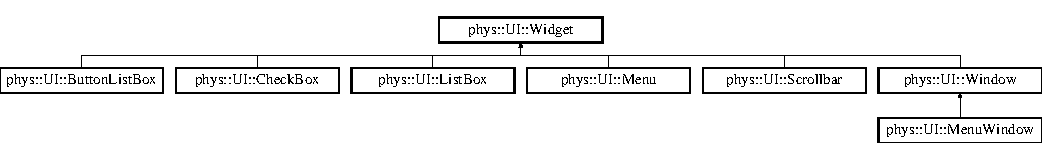
\includegraphics[height=10.000000cm]{d9/d48/classphys_1_1UI_1_1Widget}
\end{center}
\end{figure}
\subsubsection*{Public Types}
\begin{DoxyCompactItemize}
\item 
enum {\bfseries WidgetType} \{ \par
{\bfseries ButtonListBox}, 
{\bfseries Cell}, 
{\bfseries CellGrid}, 
{\bfseries CheckBox}, 
\par
{\bfseries DropDownMenu}, 
{\bfseries ListBox}, 
{\bfseries Menu}, 
{\bfseries MenuWindow}, 
\par
{\bfseries RadioButton}, 
{\bfseries Scrollbar}, 
{\bfseries Spinner}, 
{\bfseries TextBox}, 
\par
{\bfseries Window}
 \}
\end{DoxyCompactItemize}
\subsubsection*{Public Member Functions}
\begin{DoxyCompactItemize}
\item 
\hyperlink{classphys_1_1UI_1_1Widget_a7f992cc7513f1e41795b3569aa8faced}{Widget} (const \hyperlink{namespacephys_aa03900411993de7fbfec4789bc1d392e}{String} \&name, \hyperlink{classphys_1_1UI_1_1Layer}{Layer} $\ast$parent)
\begin{DoxyCompactList}\small\item\em Standard initialization constructor. \item\end{DoxyCompactList}\item 
\hypertarget{classphys_1_1UI_1_1Widget_a95bde61e93544334b376938274617d15}{
virtual \hyperlink{classphys_1_1UI_1_1Widget_a95bde61e93544334b376938274617d15}{$\sim$Widget} ()}
\label{d9/d48/classphys_1_1UI_1_1Widget_a95bde61e93544334b376938274617d15}

\begin{DoxyCompactList}\small\item\em Standard destructor. \item\end{DoxyCompactList}\item 
virtual void \hyperlink{classphys_1_1UI_1_1Widget_ab049233d8d5522a6ab42654b8924a3e0}{SetVisible} (bool visible)=0
\begin{DoxyCompactList}\small\item\em Sets the visibility of this widget. \item\end{DoxyCompactList}\item 
virtual bool \hyperlink{classphys_1_1UI_1_1Widget_aaf1a1bd31b8e626467ce9cdb69bdf7ac}{IsVisible} ()=0
\begin{DoxyCompactList}\small\item\em Gets the visibility of this widget. \item\end{DoxyCompactList}\item 
\hypertarget{classphys_1_1UI_1_1Widget_aa53e64903afc4a1fecd066c814b6c8d4}{
virtual void \hyperlink{classphys_1_1UI_1_1Widget_aa53e64903afc4a1fecd066c814b6c8d4}{Show} ()=0}
\label{d9/d48/classphys_1_1UI_1_1Widget_aa53e64903afc4a1fecd066c814b6c8d4}

\begin{DoxyCompactList}\small\item\em Forces this widget to be shown. \item\end{DoxyCompactList}\item 
\hypertarget{classphys_1_1UI_1_1Widget_abc8e3f88f780e3b36b38086c45311795}{
virtual void \hyperlink{classphys_1_1UI_1_1Widget_abc8e3f88f780e3b36b38086c45311795}{Hide} ()=0}
\label{d9/d48/classphys_1_1UI_1_1Widget_abc8e3f88f780e3b36b38086c45311795}

\begin{DoxyCompactList}\small\item\em Forces this widget to hide. \item\end{DoxyCompactList}\item 
WidgetType \hyperlink{classphys_1_1UI_1_1Widget_a76337b279bd372ce225f94ab1da191ea}{GetType} () const 
\begin{DoxyCompactList}\small\item\em Gets the type of widget this is. \item\end{DoxyCompactList}\item 
virtual bool \hyperlink{classphys_1_1UI_1_1Widget_af8498cbe2d6cf37115cf8ade52e22557}{IsInputCaptureWidget} ()
\begin{DoxyCompactList}\small\item\em Checks if this is an input capturing widget. \item\end{DoxyCompactList}\item 
virtual \hyperlink{namespacephys_aa03900411993de7fbfec4789bc1d392e}{String} \& \hyperlink{classphys_1_1UI_1_1Widget_a35d6e7ce60a9b295d8659345627cf7e0}{GetName} ()
\begin{DoxyCompactList}\small\item\em Gets the name of this widget. \item\end{DoxyCompactList}\item 
virtual bool \hyperlink{classphys_1_1UI_1_1Widget_a613df6dbb42efe139d185043a00259dc}{CheckMouseHover} ()=0
\begin{DoxyCompactList}\small\item\em Checks to see if the current mouse position is over this widget. \item\end{DoxyCompactList}\item 
virtual void \hyperlink{classphys_1_1UI_1_1Widget_a3ef894be2c0868105b2bf495ae944d00}{SetPosition} (const \hyperlink{classphys_1_1Vector2}{Vector2} \&Position)=0
\begin{DoxyCompactList}\small\item\em Sets the relative position of this widget. \item\end{DoxyCompactList}\item 
virtual \hyperlink{classphys_1_1Vector2}{Vector2} \hyperlink{classphys_1_1UI_1_1Widget_a3e464b028b0d1b5755923b8790260c33}{GetPosition} ()=0
\begin{DoxyCompactList}\small\item\em Gets the relative position of this widget. \item\end{DoxyCompactList}\item 
virtual void \hyperlink{classphys_1_1UI_1_1Widget_a77727351d98b10f1f4eb45048cb882e3}{SetActualPosition} (const \hyperlink{classphys_1_1Vector2}{Vector2} \&Position)=0
\begin{DoxyCompactList}\small\item\em Sets the pixel position of this widget. \item\end{DoxyCompactList}\item 
virtual \hyperlink{classphys_1_1Vector2}{Vector2} \hyperlink{classphys_1_1UI_1_1Widget_a0a29fecff7f56d7909f65fd63b0990e7}{GetActualPosition} ()=0
\begin{DoxyCompactList}\small\item\em Sets the pixel position of this widget. \item\end{DoxyCompactList}\item 
virtual void \hyperlink{classphys_1_1UI_1_1Widget_a00f73c12583d25a75c089f944075b24d}{SetSize} (const \hyperlink{classphys_1_1Vector2}{Vector2} \&Size)=0
\begin{DoxyCompactList}\small\item\em Sets the relative size of this widget. \item\end{DoxyCompactList}\item 
virtual \hyperlink{classphys_1_1Vector2}{Vector2} \hyperlink{classphys_1_1UI_1_1Widget_a07039c19e57de314147ce066417da0a2}{GetSize} ()=0
\begin{DoxyCompactList}\small\item\em Gets the relative size of this widget. \item\end{DoxyCompactList}\item 
virtual void \hyperlink{classphys_1_1UI_1_1Widget_acda63a62fa158d5fe00c86f50e5c120d}{SetActualSize} (const \hyperlink{classphys_1_1Vector2}{Vector2} \&Size)=0
\begin{DoxyCompactList}\small\item\em Sets the pixel size of this widget. \item\end{DoxyCompactList}\item 
virtual \hyperlink{classphys_1_1Vector2}{Vector2} \hyperlink{classphys_1_1UI_1_1Widget_af3a685621ed220748c0940ea38c96ed2}{GetActualSize} ()=0
\begin{DoxyCompactList}\small\item\em Sets the pixel size of this widget. \item\end{DoxyCompactList}\item 
virtual void \hyperlink{classphys_1_1UI_1_1Widget_acbda7003549c6caac46078c034657929}{UpdateDimensions} (const \hyperlink{classphys_1_1Vector2}{Vector2} \&OldViewportSize)
\begin{DoxyCompactList}\small\item\em Updates the dimensions of this widget to match those of the new screen size. \item\end{DoxyCompactList}\item 
virtual \hyperlink{classphys_1_1UI_1_1Button}{Button} $\ast$ \hyperlink{classphys_1_1UI_1_1Widget_ab563c13db418e4c3ff0a0dd766550251}{GetHoveredButton} ()
\begin{DoxyCompactList}\small\item\em Gets the hovered button within this widget, if any. \item\end{DoxyCompactList}\item 
virtual \hyperlink{classphys_1_1UI_1_1Widget}{Widget} $\ast$ \hyperlink{classphys_1_1UI_1_1Widget_a38764b73bc6087e2611660735840ba3f}{GetHoveredSubWidget} ()
\begin{DoxyCompactList}\small\item\em Gets the hovered sub-\/widget within this widget, if any. \item\end{DoxyCompactList}\item 
virtual \hyperlink{classphys_1_1UI_1_1Layer}{Layer} $\ast$ \hyperlink{classphys_1_1UI_1_1Widget_a33f97d7da0ac48a35006cb71676e6c2e}{GetLayer} ()
\begin{DoxyCompactList}\small\item\em Gets the layer this widget belongs to. \item\end{DoxyCompactList}\item 
virtual \hyperlink{classphys_1_1UI_1_1InputCaptureData}{InputCaptureData} $\ast$ \hyperlink{classphys_1_1UI_1_1Widget_a900184fbe7af51581d6bddafb45d953a}{GetInputCaptureData} ()
\begin{DoxyCompactList}\small\item\em Gets the data determining what input should be captured. \item\end{DoxyCompactList}\end{DoxyCompactItemize}
\subsubsection*{Protected Member Functions}
\begin{DoxyCompactItemize}
\item 
\hypertarget{classphys_1_1UI_1_1Widget_a1806425fcd684c2f0d50cd0ef4a6b0da}{
virtual void \hyperlink{classphys_1_1UI_1_1Widget_a1806425fcd684c2f0d50cd0ef4a6b0da}{Update} (bool Force=false)=0}
\label{d9/d48/classphys_1_1UI_1_1Widget_a1806425fcd684c2f0d50cd0ef4a6b0da}

\begin{DoxyCompactList}\small\item\em For use with widget update/automation. \item\end{DoxyCompactList}\item 
\hypertarget{classphys_1_1UI_1_1Widget_a3472e5d0f8281e704d67d419980cd918}{
virtual void \hyperlink{classphys_1_1UI_1_1Widget_a3472e5d0f8281e704d67d419980cd918}{SubWidgetUpdate} (bool Force=false)}
\label{d9/d48/classphys_1_1UI_1_1Widget_a3472e5d0f8281e704d67d419980cd918}

\begin{DoxyCompactList}\small\item\em For use with sub-\/widget update/automation. \item\end{DoxyCompactList}\item 
\hypertarget{classphys_1_1UI_1_1Widget_a4a7e18c48a7cd230fd4a0aa274c6a654}{
virtual void \hyperlink{classphys_1_1UI_1_1Widget_a4a7e18c48a7cd230fd4a0aa274c6a654}{SubWidgetFocusUpdate} (bool Force=false)}
\label{d9/d48/classphys_1_1UI_1_1Widget_a4a7e18c48a7cd230fd4a0aa274c6a654}

\begin{DoxyCompactList}\small\item\em For use with sub-\/widget update/automation when the mouse isn't hovered. \item\end{DoxyCompactList}\item 
\hypertarget{classphys_1_1UI_1_1Widget_ac51b863fb1a9c5ebaef1386b77dbda99}{
virtual void \hyperlink{classphys_1_1UI_1_1Widget_ac51b863fb1a9c5ebaef1386b77dbda99}{ProcessCapturedInputs} ()}
\label{d9/d48/classphys_1_1UI_1_1Widget_ac51b863fb1a9c5ebaef1386b77dbda99}

\begin{DoxyCompactList}\small\item\em Processes the captured inputs. This is an empty function and should be overridden if making an input capturing widget. \item\end{DoxyCompactList}\end{DoxyCompactItemize}
\subsubsection*{Protected Attributes}
\begin{DoxyCompactItemize}
\item 
\hypertarget{classphys_1_1UI_1_1Widget_a812fbbc32757b89af66053ea9b0f956c}{
\hyperlink{classphys_1_1UIManager}{UIManager} $\ast$ {\bfseries Manager}}
\label{d9/d48/classphys_1_1UI_1_1Widget_a812fbbc32757b89af66053ea9b0f956c}

\item 
\hypertarget{classphys_1_1UI_1_1Widget_aa86407b2762dd0e164bccdd571c184ff}{
\hyperlink{classphys_1_1UI_1_1Layer}{Layer} $\ast$ {\bfseries Parent}}
\label{d9/d48/classphys_1_1UI_1_1Widget_aa86407b2762dd0e164bccdd571c184ff}

\item 
\hypertarget{classphys_1_1UI_1_1Widget_a94dbd052a2983aef7c719053dc182810}{
\hyperlink{classphys_1_1UI_1_1InputCaptureData}{InputCaptureData} $\ast$ {\bfseries CaptureData}}
\label{d9/d48/classphys_1_1UI_1_1Widget_a94dbd052a2983aef7c719053dc182810}

\item 
\hypertarget{classphys_1_1UI_1_1Widget_a932ea9853ff5d6d03d3128f79832fe67}{
\hyperlink{classphys_1_1UI_1_1Button}{UI::Button} $\ast$ {\bfseries HoveredButton}}
\label{d9/d48/classphys_1_1UI_1_1Widget_a932ea9853ff5d6d03d3128f79832fe67}

\item 
\hypertarget{classphys_1_1UI_1_1Widget_a8a1940556d7fd20c937671b2d87a70c9}{
\hyperlink{classphys_1_1UI_1_1Widget}{UI::Widget} $\ast$ {\bfseries HoveredSubWidget}}
\label{d9/d48/classphys_1_1UI_1_1Widget_a8a1940556d7fd20c937671b2d87a70c9}

\item 
\hypertarget{classphys_1_1UI_1_1Widget_accfbf9586fddb6d31fee3e59b9b1628c}{
\hyperlink{classphys_1_1UI_1_1Widget}{UI::Widget} $\ast$ {\bfseries SubWidgetFocus}}
\label{d9/d48/classphys_1_1UI_1_1Widget_accfbf9586fddb6d31fee3e59b9b1628c}

\item 
\hypertarget{classphys_1_1UI_1_1Widget_a752b4b76947c1e55d8a6f74ab772b875}{
bool {\bfseries Visible}}
\label{d9/d48/classphys_1_1UI_1_1Widget_a752b4b76947c1e55d8a6f74ab772b875}

\item 
\hypertarget{classphys_1_1UI_1_1Widget_a9b7d9a6919cf49639585634090c09ec7}{
\hyperlink{classphys_1_1Vector2}{Vector2} {\bfseries RelPosition}}
\label{d9/d48/classphys_1_1UI_1_1Widget_a9b7d9a6919cf49639585634090c09ec7}

\item 
\hypertarget{classphys_1_1UI_1_1Widget_a0b239b76dc82d6bf5c5c3fa268f83f3e}{
\hyperlink{classphys_1_1Vector2}{Vector2} {\bfseries RelSize}}
\label{d9/d48/classphys_1_1UI_1_1Widget_a0b239b76dc82d6bf5c5c3fa268f83f3e}

\item 
\hypertarget{classphys_1_1UI_1_1Widget_af957da7e0342010f3dad1c7b4a73f334}{
WidgetType {\bfseries Type}}
\label{d9/d48/classphys_1_1UI_1_1Widget_af957da7e0342010f3dad1c7b4a73f334}

\item 
\hypertarget{classphys_1_1UI_1_1Widget_a863f635b86ec75076e4c3978dc427679}{
\hyperlink{namespacephys_aa03900411993de7fbfec4789bc1d392e}{String} {\bfseries Name}}
\label{d9/d48/classphys_1_1UI_1_1Widget_a863f635b86ec75076e4c3978dc427679}

\end{DoxyCompactItemize}
\subsubsection*{Friends}
\begin{DoxyCompactItemize}
\item 
\hypertarget{classphys_1_1UI_1_1Widget_a4b52bf8c4d934bf192ccfc8198b55394}{
class \hyperlink{classphys_1_1UI_1_1Widget_a4b52bf8c4d934bf192ccfc8198b55394}{phys::UIManager}}
\label{d9/d48/classphys_1_1UI_1_1Widget_a4b52bf8c4d934bf192ccfc8198b55394}

\end{DoxyCompactItemize}


\subsubsection{Detailed Description}
This class is the base class for all widgets. 

Definition at line 97 of file uiwidget.h.



\subsubsection{Constructor \& Destructor Documentation}
\hypertarget{classphys_1_1UI_1_1Widget_a7f992cc7513f1e41795b3569aa8faced}{
\index{phys::UI::Widget@{phys::UI::Widget}!Widget@{Widget}}
\index{Widget@{Widget}!phys::UI::Widget@{phys::UI::Widget}}
\paragraph[{Widget}]{\setlength{\rightskip}{0pt plus 5cm}phys::UI::Widget::Widget (
\begin{DoxyParamCaption}
\item[{const {\bf String} \&}]{name, }
\item[{{\bf Layer} $\ast$}]{parent}
\end{DoxyParamCaption}
)}\hfill}
\label{d9/d48/classphys_1_1UI_1_1Widget_a7f992cc7513f1e41795b3569aa8faced}


Standard initialization constructor. 


\begin{DoxyParams}{Parameters}
{\em parent} & The parent layer that created this widget. \\
\hline
{\em name} & The Name for the \hyperlink{classphys_1_1UI_1_1Widget}{Widget}. \\
\hline
\end{DoxyParams}


Definition at line 96 of file uiwidget.cpp.



\subsubsection{Member Function Documentation}
\hypertarget{classphys_1_1UI_1_1Widget_a613df6dbb42efe139d185043a00259dc}{
\index{phys::UI::Widget@{phys::UI::Widget}!CheckMouseHover@{CheckMouseHover}}
\index{CheckMouseHover@{CheckMouseHover}!phys::UI::Widget@{phys::UI::Widget}}
\paragraph[{CheckMouseHover}]{\setlength{\rightskip}{0pt plus 5cm}virtual bool phys::UI::Widget::CheckMouseHover (
\begin{DoxyParamCaption}
{}
\end{DoxyParamCaption}
)\hspace{0.3cm}{\ttfamily  \mbox{[}pure virtual\mbox{]}}}\hfill}
\label{d9/d48/classphys_1_1UI_1_1Widget_a613df6dbb42efe139d185043a00259dc}


Checks to see if the current mouse position is over this widget. 

\begin{DoxyReturn}{Returns}
Returns a bool value, true if the mouse is over this widget, false if it's not. 
\end{DoxyReturn}


Implemented in \hyperlink{classphys_1_1UI_1_1ButtonListBox_aaa8b11b174a0475cadee3d3349ef1a58}{phys::UI::ButtonListBox}, \hyperlink{classphys_1_1UI_1_1Cell_aff6472ccb5d6d7bd3e7d3a967c67674d}{phys::UI::Cell}, \hyperlink{classphys_1_1UI_1_1CellGrid_a9c5f899c7db6c24d9aa2b03e59e5f0f0}{phys::UI::CellGrid}, \hyperlink{classphys_1_1UI_1_1CheckBox_a3c9b10c692dfb62dedbd091dac12c115}{phys::UI::CheckBox}, \hyperlink{classphys_1_1UI_1_1ListBox_a789faeb98d98bb4d4d89cae8c53d4bc0}{phys::UI::ListBox}, \hyperlink{classphys_1_1UI_1_1Menu_af2514d2614322856f604be2e167d0872}{phys::UI::Menu}, \hyperlink{classphys_1_1UI_1_1PagedCellGrid_a859ed3c174faf86962df4d0fd2b43fab}{phys::UI::PagedCellGrid}, \hyperlink{classphys_1_1UI_1_1Scrollbar_a8afdd63e36a7fdc15bd8660d9800f2c5}{phys::UI::Scrollbar}, \hyperlink{classphys_1_1UI_1_1ScrolledCellGrid_a976e99e204f912d82712872e4e80b833}{phys::UI::ScrolledCellGrid}, \hyperlink{classphys_1_1UI_1_1Spinner_ae594a38213702563841f5817609c492e}{phys::UI::Spinner}, and \hyperlink{classphys_1_1UI_1_1Window_a771bc9e43c0492ab179d8126c30665cf}{phys::UI::Window}.

\hypertarget{classphys_1_1UI_1_1Widget_a0a29fecff7f56d7909f65fd63b0990e7}{
\index{phys::UI::Widget@{phys::UI::Widget}!GetActualPosition@{GetActualPosition}}
\index{GetActualPosition@{GetActualPosition}!phys::UI::Widget@{phys::UI::Widget}}
\paragraph[{GetActualPosition}]{\setlength{\rightskip}{0pt plus 5cm}virtual {\bf Vector2} phys::UI::Widget::GetActualPosition (
\begin{DoxyParamCaption}
{}
\end{DoxyParamCaption}
)\hspace{0.3cm}{\ttfamily  \mbox{[}pure virtual\mbox{]}}}\hfill}
\label{d9/d48/classphys_1_1UI_1_1Widget_a0a29fecff7f56d7909f65fd63b0990e7}


Sets the pixel position of this widget. 

\begin{DoxyReturn}{Returns}
Returns a vector2 representing the pixel position of this widget. 
\end{DoxyReturn}


Implemented in \hyperlink{classphys_1_1UI_1_1ButtonListBox_addc5d7c6ab2a48ffa0d4b2e46c20d9a5}{phys::UI::ButtonListBox}, \hyperlink{classphys_1_1UI_1_1Cell_a1b0deb9738bc4da73e0be4dd355b23fb}{phys::UI::Cell}, \hyperlink{classphys_1_1UI_1_1CellGrid_a1ead8b427b5989ec137aa0ca8e017f73}{phys::UI::CellGrid}, \hyperlink{classphys_1_1UI_1_1CheckBox_a33bedaa00456be8ca0e9b2eafcd5b21a}{phys::UI::CheckBox}, \hyperlink{classphys_1_1UI_1_1ListBox_a44046453283fb2c54e10dc868705352a}{phys::UI::ListBox}, \hyperlink{classphys_1_1UI_1_1Menu_a74a1b8e9b1c5d36c12e5a0a7f813c40a}{phys::UI::Menu}, \hyperlink{classphys_1_1UI_1_1Scrollbar_a73337985c0f1f173e253c88705ae5d6e}{phys::UI::Scrollbar}, \hyperlink{classphys_1_1UI_1_1Spinner_a7ee24e3f5c11550950696a2c9094d716}{phys::UI::Spinner}, and \hyperlink{classphys_1_1UI_1_1Window_a811fb495bc698752e03778b18f2b1a30}{phys::UI::Window}.

\hypertarget{classphys_1_1UI_1_1Widget_af3a685621ed220748c0940ea38c96ed2}{
\index{phys::UI::Widget@{phys::UI::Widget}!GetActualSize@{GetActualSize}}
\index{GetActualSize@{GetActualSize}!phys::UI::Widget@{phys::UI::Widget}}
\paragraph[{GetActualSize}]{\setlength{\rightskip}{0pt plus 5cm}virtual {\bf Vector2} phys::UI::Widget::GetActualSize (
\begin{DoxyParamCaption}
{}
\end{DoxyParamCaption}
)\hspace{0.3cm}{\ttfamily  \mbox{[}pure virtual\mbox{]}}}\hfill}
\label{d9/d48/classphys_1_1UI_1_1Widget_af3a685621ed220748c0940ea38c96ed2}


Sets the pixel size of this widget. 

\begin{DoxyReturn}{Returns}
Returns a vector2 representing the pixel size of this widget. 
\end{DoxyReturn}


Implemented in \hyperlink{classphys_1_1UI_1_1ButtonListBox_a77d992f8858bf9b9eeb190dd1ea8a4fd}{phys::UI::ButtonListBox}, \hyperlink{classphys_1_1UI_1_1Cell_a6301ce41a7a44a97de36fb54388ad430}{phys::UI::Cell}, \hyperlink{classphys_1_1UI_1_1CellGrid_ad0ea7915446ba7821212e6a43aede7e1}{phys::UI::CellGrid}, \hyperlink{classphys_1_1UI_1_1CheckBox_aa13946ced3947a13f8f30dd97ffba245}{phys::UI::CheckBox}, \hyperlink{classphys_1_1UI_1_1ListBox_a23133ed4a98994d838acee4c6a981e04}{phys::UI::ListBox}, \hyperlink{classphys_1_1UI_1_1Menu_af7566b83c50a4a02ac78d174d7c61817}{phys::UI::Menu}, \hyperlink{classphys_1_1UI_1_1Scrollbar_a2b3d791cbbe4c787f284d8b12a0edf27}{phys::UI::Scrollbar}, \hyperlink{classphys_1_1UI_1_1Spinner_af2843083a652f2d7ca6e929582f501fd}{phys::UI::Spinner}, and \hyperlink{classphys_1_1UI_1_1Window_a22f5ca800e44c5e2cfeed59c243b03ed}{phys::UI::Window}.

\hypertarget{classphys_1_1UI_1_1Widget_ab563c13db418e4c3ff0a0dd766550251}{
\index{phys::UI::Widget@{phys::UI::Widget}!GetHoveredButton@{GetHoveredButton}}
\index{GetHoveredButton@{GetHoveredButton}!phys::UI::Widget@{phys::UI::Widget}}
\paragraph[{GetHoveredButton}]{\setlength{\rightskip}{0pt plus 5cm}{\bf Button} $\ast$ phys::UI::Widget::GetHoveredButton (
\begin{DoxyParamCaption}
{}
\end{DoxyParamCaption}
)\hspace{0.3cm}{\ttfamily  \mbox{[}virtual\mbox{]}}}\hfill}
\label{d9/d48/classphys_1_1UI_1_1Widget_ab563c13db418e4c3ff0a0dd766550251}


Gets the hovered button within this widget, if any. 

\begin{DoxyReturn}{Returns}
Returns a pointer to the button within this widget the mouse is hovering over, or NULL if none. 
\end{DoxyReturn}


Definition at line 152 of file uiwidget.cpp.

\hypertarget{classphys_1_1UI_1_1Widget_a38764b73bc6087e2611660735840ba3f}{
\index{phys::UI::Widget@{phys::UI::Widget}!GetHoveredSubWidget@{GetHoveredSubWidget}}
\index{GetHoveredSubWidget@{GetHoveredSubWidget}!phys::UI::Widget@{phys::UI::Widget}}
\paragraph[{GetHoveredSubWidget}]{\setlength{\rightskip}{0pt plus 5cm}{\bf Widget} $\ast$ phys::UI::Widget::GetHoveredSubWidget (
\begin{DoxyParamCaption}
{}
\end{DoxyParamCaption}
)\hspace{0.3cm}{\ttfamily  \mbox{[}virtual\mbox{]}}}\hfill}
\label{d9/d48/classphys_1_1UI_1_1Widget_a38764b73bc6087e2611660735840ba3f}


Gets the hovered sub-\/widget within this widget, if any. 

\begin{DoxyReturn}{Returns}
Returns a pointer to the sub-\/widget within this widget the mouse is hovering over, or NULL if none. 
\end{DoxyReturn}


Definition at line 157 of file uiwidget.cpp.

\hypertarget{classphys_1_1UI_1_1Widget_a900184fbe7af51581d6bddafb45d953a}{
\index{phys::UI::Widget@{phys::UI::Widget}!GetInputCaptureData@{GetInputCaptureData}}
\index{GetInputCaptureData@{GetInputCaptureData}!phys::UI::Widget@{phys::UI::Widget}}
\paragraph[{GetInputCaptureData}]{\setlength{\rightskip}{0pt plus 5cm}{\bf InputCaptureData} $\ast$ phys::UI::Widget::GetInputCaptureData (
\begin{DoxyParamCaption}
{}
\end{DoxyParamCaption}
)\hspace{0.3cm}{\ttfamily  \mbox{[}virtual\mbox{]}}}\hfill}
\label{d9/d48/classphys_1_1UI_1_1Widget_a900184fbe7af51581d6bddafb45d953a}


Gets the data determining what input should be captured. 

\begin{DoxyReturn}{Returns}
Returns a pointer to the \hyperlink{classphys_1_1UI_1_1InputCaptureData}{InputCaptureData}, or NULL if this widget doesn't capture data. 
\end{DoxyReturn}


Definition at line 167 of file uiwidget.cpp.

\hypertarget{classphys_1_1UI_1_1Widget_a33f97d7da0ac48a35006cb71676e6c2e}{
\index{phys::UI::Widget@{phys::UI::Widget}!GetLayer@{GetLayer}}
\index{GetLayer@{GetLayer}!phys::UI::Widget@{phys::UI::Widget}}
\paragraph[{GetLayer}]{\setlength{\rightskip}{0pt plus 5cm}{\bf Layer} $\ast$ phys::UI::Widget::GetLayer (
\begin{DoxyParamCaption}
{}
\end{DoxyParamCaption}
)\hspace{0.3cm}{\ttfamily  \mbox{[}virtual\mbox{]}}}\hfill}
\label{d9/d48/classphys_1_1UI_1_1Widget_a33f97d7da0ac48a35006cb71676e6c2e}


Gets the layer this widget belongs to. 

\begin{DoxyReturn}{Returns}
Returns a pointer to the layer this eidget belongs to. 
\end{DoxyReturn}


Definition at line 162 of file uiwidget.cpp.

\hypertarget{classphys_1_1UI_1_1Widget_a35d6e7ce60a9b295d8659345627cf7e0}{
\index{phys::UI::Widget@{phys::UI::Widget}!GetName@{GetName}}
\index{GetName@{GetName}!phys::UI::Widget@{phys::UI::Widget}}
\paragraph[{GetName}]{\setlength{\rightskip}{0pt plus 5cm}{\bf String} \& phys::UI::Widget::GetName (
\begin{DoxyParamCaption}
{}
\end{DoxyParamCaption}
)\hspace{0.3cm}{\ttfamily  \mbox{[}virtual\mbox{]}}}\hfill}
\label{d9/d48/classphys_1_1UI_1_1Widget_a35d6e7ce60a9b295d8659345627cf7e0}


Gets the name of this widget. 

\begin{DoxyReturn}{Returns}
Returns a String containing the name of this widget. 
\end{DoxyReturn}


Definition at line 140 of file uiwidget.cpp.

\hypertarget{classphys_1_1UI_1_1Widget_a3e464b028b0d1b5755923b8790260c33}{
\index{phys::UI::Widget@{phys::UI::Widget}!GetPosition@{GetPosition}}
\index{GetPosition@{GetPosition}!phys::UI::Widget@{phys::UI::Widget}}
\paragraph[{GetPosition}]{\setlength{\rightskip}{0pt plus 5cm}virtual {\bf Vector2} phys::UI::Widget::GetPosition (
\begin{DoxyParamCaption}
{}
\end{DoxyParamCaption}
)\hspace{0.3cm}{\ttfamily  \mbox{[}pure virtual\mbox{]}}}\hfill}
\label{d9/d48/classphys_1_1UI_1_1Widget_a3e464b028b0d1b5755923b8790260c33}


Gets the relative position of this widget. 

The position is relative to the screen size. Values range from 0.0 to 1.0. \begin{DoxyReturn}{Returns}
Returns a vector2 representing the relative position of this widget. 
\end{DoxyReturn}


Implemented in \hyperlink{classphys_1_1UI_1_1ButtonListBox_ab7834542f8940adba8df6b1eace92e95}{phys::UI::ButtonListBox}, \hyperlink{classphys_1_1UI_1_1Cell_a17475dbdde2d71be3d774f0402792f0d}{phys::UI::Cell}, \hyperlink{classphys_1_1UI_1_1CellGrid_a6b7fcbfd8a965e69c6e3e92d474f121f}{phys::UI::CellGrid}, \hyperlink{classphys_1_1UI_1_1CheckBox_a8a8630b27ab769b6e42657c5388ec7fe}{phys::UI::CheckBox}, \hyperlink{classphys_1_1UI_1_1ListBox_af688db0628a5588865a890584f754b02}{phys::UI::ListBox}, \hyperlink{classphys_1_1UI_1_1Menu_a3c19fe2596fe4049325cc580daa70387}{phys::UI::Menu}, \hyperlink{classphys_1_1UI_1_1Scrollbar_ad049af26ff2247cfcd988cb5639fa003}{phys::UI::Scrollbar}, \hyperlink{classphys_1_1UI_1_1Spinner_a0cfed1bd9532351eac373b0f23495225}{phys::UI::Spinner}, and \hyperlink{classphys_1_1UI_1_1Window_a29fca96d9a2dab29d77a36d6a329f306}{phys::UI::Window}.

\hypertarget{classphys_1_1UI_1_1Widget_a07039c19e57de314147ce066417da0a2}{
\index{phys::UI::Widget@{phys::UI::Widget}!GetSize@{GetSize}}
\index{GetSize@{GetSize}!phys::UI::Widget@{phys::UI::Widget}}
\paragraph[{GetSize}]{\setlength{\rightskip}{0pt plus 5cm}virtual {\bf Vector2} phys::UI::Widget::GetSize (
\begin{DoxyParamCaption}
{}
\end{DoxyParamCaption}
)\hspace{0.3cm}{\ttfamily  \mbox{[}pure virtual\mbox{]}}}\hfill}
\label{d9/d48/classphys_1_1UI_1_1Widget_a07039c19e57de314147ce066417da0a2}


Gets the relative size of this widget. 

The size is relative to the screen size. Values range from 0.0 to 1.0. \begin{DoxyReturn}{Returns}
Returns a vector2 representing the relative size of this widget. 
\end{DoxyReturn}


Implemented in \hyperlink{classphys_1_1UI_1_1ButtonListBox_a0084510b0b9c53761e5b4a45f65604ab}{phys::UI::ButtonListBox}, \hyperlink{classphys_1_1UI_1_1Cell_ab8288a97a63aad7cc02f32541b1b7351}{phys::UI::Cell}, \hyperlink{classphys_1_1UI_1_1CellGrid_aa0ad4f1e0159f8c6ca3928595dffd837}{phys::UI::CellGrid}, \hyperlink{classphys_1_1UI_1_1CheckBox_a99c6ab5087522fbd4825032b9a058585}{phys::UI::CheckBox}, \hyperlink{classphys_1_1UI_1_1ListBox_a7af2cced185d63be6a62d5122c700d81}{phys::UI::ListBox}, \hyperlink{classphys_1_1UI_1_1Menu_a81781199a62bbe7c2e7693ef301223b4}{phys::UI::Menu}, \hyperlink{classphys_1_1UI_1_1Scrollbar_aff97ce371ee21fcf3b648dcf8b38e055}{phys::UI::Scrollbar}, \hyperlink{classphys_1_1UI_1_1Spinner_a670d8ff577a8feb6df6f507843f08756}{phys::UI::Spinner}, and \hyperlink{classphys_1_1UI_1_1Window_a9946100eb6e6e985921bbea9e87cede3}{phys::UI::Window}.

\hypertarget{classphys_1_1UI_1_1Widget_a76337b279bd372ce225f94ab1da191ea}{
\index{phys::UI::Widget@{phys::UI::Widget}!GetType@{GetType}}
\index{GetType@{GetType}!phys::UI::Widget@{phys::UI::Widget}}
\paragraph[{GetType}]{\setlength{\rightskip}{0pt plus 5cm}Widget::WidgetType phys::UI::Widget::GetType (
\begin{DoxyParamCaption}
{}
\end{DoxyParamCaption}
) const}\hfill}
\label{d9/d48/classphys_1_1UI_1_1Widget_a76337b279bd372ce225f94ab1da191ea}


Gets the type of widget this is. 

\begin{DoxyReturn}{Returns}
Returns an enum value representing the type of widget this is. 
\end{DoxyReturn}


Definition at line 130 of file uiwidget.cpp.

\hypertarget{classphys_1_1UI_1_1Widget_af8498cbe2d6cf37115cf8ade52e22557}{
\index{phys::UI::Widget@{phys::UI::Widget}!IsInputCaptureWidget@{IsInputCaptureWidget}}
\index{IsInputCaptureWidget@{IsInputCaptureWidget}!phys::UI::Widget@{phys::UI::Widget}}
\paragraph[{IsInputCaptureWidget}]{\setlength{\rightskip}{0pt plus 5cm}bool phys::UI::Widget::IsInputCaptureWidget (
\begin{DoxyParamCaption}
{}
\end{DoxyParamCaption}
)\hspace{0.3cm}{\ttfamily  \mbox{[}virtual\mbox{]}}}\hfill}
\label{d9/d48/classphys_1_1UI_1_1Widget_af8498cbe2d6cf37115cf8ade52e22557}


Checks if this is an input capturing widget. 

\begin{DoxyReturn}{Returns}
Returns a bool indicating whether or not this widget will capture input. 
\end{DoxyReturn}


Definition at line 135 of file uiwidget.cpp.

\hypertarget{classphys_1_1UI_1_1Widget_aaf1a1bd31b8e626467ce9cdb69bdf7ac}{
\index{phys::UI::Widget@{phys::UI::Widget}!IsVisible@{IsVisible}}
\index{IsVisible@{IsVisible}!phys::UI::Widget@{phys::UI::Widget}}
\paragraph[{IsVisible}]{\setlength{\rightskip}{0pt plus 5cm}virtual bool phys::UI::Widget::IsVisible (
\begin{DoxyParamCaption}
{}
\end{DoxyParamCaption}
)\hspace{0.3cm}{\ttfamily  \mbox{[}pure virtual\mbox{]}}}\hfill}
\label{d9/d48/classphys_1_1UI_1_1Widget_aaf1a1bd31b8e626467ce9cdb69bdf7ac}


Gets the visibility of this widget. 

\begin{DoxyReturn}{Returns}
Returns a bool representing the visibility of this widget. 
\end{DoxyReturn}


Implemented in \hyperlink{classphys_1_1UI_1_1ButtonListBox_a1282a1494079e47b48c8e3296b1a8bb0}{phys::UI::ButtonListBox}, \hyperlink{classphys_1_1UI_1_1Cell_a77625842ac8ad87bd5b5a7f6ed0590b8}{phys::UI::Cell}, \hyperlink{classphys_1_1UI_1_1CellGrid_af53601ab18e77237550c3eb97043e68c}{phys::UI::CellGrid}, \hyperlink{classphys_1_1UI_1_1CheckBox_a8a2be0cba227f0921071fb14de24f76d}{phys::UI::CheckBox}, \hyperlink{classphys_1_1UI_1_1ListBox_a638f19eb6e5a0bd3291fab1ebaccc84f}{phys::UI::ListBox}, \hyperlink{classphys_1_1UI_1_1Menu_ae23321617d7e14448e2fab3b455c3dc7}{phys::UI::Menu}, \hyperlink{classphys_1_1UI_1_1Scrollbar_a213c946ccadd3b689f59e2761a1d1848}{phys::UI::Scrollbar}, \hyperlink{classphys_1_1UI_1_1Spinner_a3bb14ddd6426debf035e65b9885bc25b}{phys::UI::Spinner}, and \hyperlink{classphys_1_1UI_1_1Window_aa1d88c50c0965510b494b51f3e5a7bf0}{phys::UI::Window}.

\hypertarget{classphys_1_1UI_1_1Widget_a77727351d98b10f1f4eb45048cb882e3}{
\index{phys::UI::Widget@{phys::UI::Widget}!SetActualPosition@{SetActualPosition}}
\index{SetActualPosition@{SetActualPosition}!phys::UI::Widget@{phys::UI::Widget}}
\paragraph[{SetActualPosition}]{\setlength{\rightskip}{0pt plus 5cm}virtual void phys::UI::Widget::SetActualPosition (
\begin{DoxyParamCaption}
\item[{const {\bf Vector2} \&}]{Position}
\end{DoxyParamCaption}
)\hspace{0.3cm}{\ttfamily  \mbox{[}pure virtual\mbox{]}}}\hfill}
\label{d9/d48/classphys_1_1UI_1_1Widget_a77727351d98b10f1f4eb45048cb882e3}


Sets the pixel position of this widget. 


\begin{DoxyParams}{Parameters}
{\em Position} & A vector2 representing the pixel position of this widget. \\
\hline
\end{DoxyParams}


Implemented in \hyperlink{classphys_1_1UI_1_1ButtonListBox_a3b027750d7d1a5b84a98fc348dee4e64}{phys::UI::ButtonListBox}, \hyperlink{classphys_1_1UI_1_1Cell_ae8b1850754b6b9ea48636b619dada5ea}{phys::UI::Cell}, \hyperlink{classphys_1_1UI_1_1CellGrid_a911ce43c124ca7ac9f02ba7d8e08d919}{phys::UI::CellGrid}, \hyperlink{classphys_1_1UI_1_1CheckBox_a186fcf91ed44c813d6dbd9cb53ff60c3}{phys::UI::CheckBox}, \hyperlink{classphys_1_1UI_1_1ListBox_a4bf1911c639429c783915ba8a543fec3}{phys::UI::ListBox}, \hyperlink{classphys_1_1UI_1_1Menu_a1d5434382755df214b169d3e9901c1e1}{phys::UI::Menu}, \hyperlink{classphys_1_1UI_1_1Scrollbar_a93dfa3232185d72f274462636a833465}{phys::UI::Scrollbar}, \hyperlink{classphys_1_1UI_1_1ScrolledCellGrid_aceff3ee36c2677d55e1a4e355611eef9}{phys::UI::ScrolledCellGrid}, \hyperlink{classphys_1_1UI_1_1Spinner_a66bc26a2252cacd71e8c409e35672909}{phys::UI::Spinner}, and \hyperlink{classphys_1_1UI_1_1Window_a45a3d0454803ce26a053f645b965d16b}{phys::UI::Window}.

\hypertarget{classphys_1_1UI_1_1Widget_acda63a62fa158d5fe00c86f50e5c120d}{
\index{phys::UI::Widget@{phys::UI::Widget}!SetActualSize@{SetActualSize}}
\index{SetActualSize@{SetActualSize}!phys::UI::Widget@{phys::UI::Widget}}
\paragraph[{SetActualSize}]{\setlength{\rightskip}{0pt plus 5cm}virtual void phys::UI::Widget::SetActualSize (
\begin{DoxyParamCaption}
\item[{const {\bf Vector2} \&}]{Size}
\end{DoxyParamCaption}
)\hspace{0.3cm}{\ttfamily  \mbox{[}pure virtual\mbox{]}}}\hfill}
\label{d9/d48/classphys_1_1UI_1_1Widget_acda63a62fa158d5fe00c86f50e5c120d}


Sets the pixel size of this widget. 


\begin{DoxyParams}{Parameters}
{\em Size} & A vector2 representing the pixel size of this widget. \\
\hline
\end{DoxyParams}


Implemented in \hyperlink{classphys_1_1UI_1_1ButtonListBox_a40f357673d774cbecae7104a02be365e}{phys::UI::ButtonListBox}, \hyperlink{classphys_1_1UI_1_1Cell_a3666c40546d1e6a225421d3bfd0288f9}{phys::UI::Cell}, \hyperlink{classphys_1_1UI_1_1CellGrid_a86a0ff7a5a916278d901bae05df01847}{phys::UI::CellGrid}, \hyperlink{classphys_1_1UI_1_1CheckBox_a623769e2a3ba24cc1a3e2e64b72edb41}{phys::UI::CheckBox}, \hyperlink{classphys_1_1UI_1_1ListBox_a742810da75f2b3889794498f05af8860}{phys::UI::ListBox}, \hyperlink{classphys_1_1UI_1_1Menu_acc3fb39539fd3c13def35be54570ae81}{phys::UI::Menu}, \hyperlink{classphys_1_1UI_1_1Scrollbar_aabdb8b727f1f84712a5f7c1fca6e830f}{phys::UI::Scrollbar}, \hyperlink{classphys_1_1UI_1_1ScrolledCellGrid_a32ee6cc683f7357afef8b7075d8b8f20}{phys::UI::ScrolledCellGrid}, \hyperlink{classphys_1_1UI_1_1Spinner_a564782cd7135a708295c51e722f22716}{phys::UI::Spinner}, and \hyperlink{classphys_1_1UI_1_1Window_a002150cd8db87283bead5f10b2310152}{phys::UI::Window}.

\hypertarget{classphys_1_1UI_1_1Widget_a3ef894be2c0868105b2bf495ae944d00}{
\index{phys::UI::Widget@{phys::UI::Widget}!SetPosition@{SetPosition}}
\index{SetPosition@{SetPosition}!phys::UI::Widget@{phys::UI::Widget}}
\paragraph[{SetPosition}]{\setlength{\rightskip}{0pt plus 5cm}virtual void phys::UI::Widget::SetPosition (
\begin{DoxyParamCaption}
\item[{const {\bf Vector2} \&}]{Position}
\end{DoxyParamCaption}
)\hspace{0.3cm}{\ttfamily  \mbox{[}pure virtual\mbox{]}}}\hfill}
\label{d9/d48/classphys_1_1UI_1_1Widget_a3ef894be2c0868105b2bf495ae944d00}


Sets the relative position of this widget. 

The position is relative to the screen size. Values range from 0.0 to 1.0. 
\begin{DoxyParams}{Parameters}
{\em Position} & A vector2 representing the relative position of this widget. \\
\hline
\end{DoxyParams}


Implemented in \hyperlink{classphys_1_1UI_1_1ButtonListBox_a9c6b0bc4eb93b53c4f7172ce3a537178}{phys::UI::ButtonListBox}, \hyperlink{classphys_1_1UI_1_1Cell_af43b353b0033d3605dad04e925363f2b}{phys::UI::Cell}, \hyperlink{classphys_1_1UI_1_1CellGrid_abf0552ebbe369f6b695f91fdaa220c20}{phys::UI::CellGrid}, \hyperlink{classphys_1_1UI_1_1CheckBox_ae0a000643e0f96f12d754a8e1e5dd04b}{phys::UI::CheckBox}, \hyperlink{classphys_1_1UI_1_1ListBox_a0c4c7141142caca342157ce4460b907d}{phys::UI::ListBox}, \hyperlink{classphys_1_1UI_1_1Menu_a53ff13bb9b850fb8196c1c0c637afbd5}{phys::UI::Menu}, \hyperlink{classphys_1_1UI_1_1Scrollbar_a4a87f32e31e8e4443c4aaec46307864e}{phys::UI::Scrollbar}, \hyperlink{classphys_1_1UI_1_1ScrolledCellGrid_aef62a124cb71b39bc73bda770741882f}{phys::UI::ScrolledCellGrid}, \hyperlink{classphys_1_1UI_1_1Spinner_a7b520a5aa26772bd15e880887d174fa6}{phys::UI::Spinner}, and \hyperlink{classphys_1_1UI_1_1Window_a17e6284d4ac5aa95f257c5168d6cc5ac}{phys::UI::Window}.

\hypertarget{classphys_1_1UI_1_1Widget_a00f73c12583d25a75c089f944075b24d}{
\index{phys::UI::Widget@{phys::UI::Widget}!SetSize@{SetSize}}
\index{SetSize@{SetSize}!phys::UI::Widget@{phys::UI::Widget}}
\paragraph[{SetSize}]{\setlength{\rightskip}{0pt plus 5cm}virtual void phys::UI::Widget::SetSize (
\begin{DoxyParamCaption}
\item[{const {\bf Vector2} \&}]{Size}
\end{DoxyParamCaption}
)\hspace{0.3cm}{\ttfamily  \mbox{[}pure virtual\mbox{]}}}\hfill}
\label{d9/d48/classphys_1_1UI_1_1Widget_a00f73c12583d25a75c089f944075b24d}


Sets the relative size of this widget. 

The size is relative to the screen size. Values range from 0.0 to 1.0. 
\begin{DoxyParams}{Parameters}
{\em Size} & A vector2 representing the relative size of this widget. \\
\hline
\end{DoxyParams}


Implemented in \hyperlink{classphys_1_1UI_1_1ButtonListBox_affc95f7b3c3753b5a89eda7f84c78fb0}{phys::UI::ButtonListBox}, \hyperlink{classphys_1_1UI_1_1Cell_a59075a5ae35c2080876fcc78a97e5b31}{phys::UI::Cell}, \hyperlink{classphys_1_1UI_1_1CellGrid_a83de47589cb02ce49882f795e9281f57}{phys::UI::CellGrid}, \hyperlink{classphys_1_1UI_1_1CheckBox_a3cacea11779470e31efb6020c22e0c54}{phys::UI::CheckBox}, \hyperlink{classphys_1_1UI_1_1ListBox_a2e1f6514f83be768dad7e357beb6ac98}{phys::UI::ListBox}, \hyperlink{classphys_1_1UI_1_1Menu_adef3f9d3351c959f711e929a5e1c8f76}{phys::UI::Menu}, \hyperlink{classphys_1_1UI_1_1Scrollbar_a5581675d3f250ed7270018e184b02b1d}{phys::UI::Scrollbar}, \hyperlink{classphys_1_1UI_1_1ScrolledCellGrid_a793a775a3603e71db5ad29686c27ae68}{phys::UI::ScrolledCellGrid}, \hyperlink{classphys_1_1UI_1_1Spinner_a01641c5ed2b360307f3056f142964bf4}{phys::UI::Spinner}, and \hyperlink{classphys_1_1UI_1_1Window_a88ed4d21758cee9afeadc4069c3e0b04}{phys::UI::Window}.

\hypertarget{classphys_1_1UI_1_1Widget_ab049233d8d5522a6ab42654b8924a3e0}{
\index{phys::UI::Widget@{phys::UI::Widget}!SetVisible@{SetVisible}}
\index{SetVisible@{SetVisible}!phys::UI::Widget@{phys::UI::Widget}}
\paragraph[{SetVisible}]{\setlength{\rightskip}{0pt plus 5cm}virtual void phys::UI::Widget::SetVisible (
\begin{DoxyParamCaption}
\item[{bool}]{visible}
\end{DoxyParamCaption}
)\hspace{0.3cm}{\ttfamily  \mbox{[}pure virtual\mbox{]}}}\hfill}
\label{d9/d48/classphys_1_1UI_1_1Widget_ab049233d8d5522a6ab42654b8924a3e0}


Sets the visibility of this widget. 


\begin{DoxyParams}{Parameters}
{\em visible} & Bool determining whether or not this widget should be visible. \\
\hline
\end{DoxyParams}


Implemented in \hyperlink{classphys_1_1UI_1_1ButtonListBox_acee378e954050801fa8fffe835441bf4}{phys::UI::ButtonListBox}, \hyperlink{classphys_1_1UI_1_1Cell_aceb2d399897a502d99c72b2e9e5c859e}{phys::UI::Cell}, \hyperlink{classphys_1_1UI_1_1CellGrid_abd1b3b422680a8b549c1c897b300da5d}{phys::UI::CellGrid}, \hyperlink{classphys_1_1UI_1_1CheckBox_aac2babdb951a7b716b5cfff9b925420f}{phys::UI::CheckBox}, \hyperlink{classphys_1_1UI_1_1ListBox_abb3c87bf6669100296c1fa4f4913ea33}{phys::UI::ListBox}, \hyperlink{classphys_1_1UI_1_1Menu_a4847e0de055a9c2f708f98742fa59a87}{phys::UI::Menu}, \hyperlink{classphys_1_1UI_1_1PagedCellGrid_a76ff4b649f4687203ba9d1473474ce99}{phys::UI::PagedCellGrid}, \hyperlink{classphys_1_1UI_1_1Scrollbar_a2d8997e0bbbb1c17af5128fea98fb1e4}{phys::UI::Scrollbar}, \hyperlink{classphys_1_1UI_1_1ScrolledCellGrid_aef5b78f205e75d33fff05623a1b61aa4}{phys::UI::ScrolledCellGrid}, \hyperlink{classphys_1_1UI_1_1Spinner_a4fddc28f38174c4a89761efa00ae88c3}{phys::UI::Spinner}, and \hyperlink{classphys_1_1UI_1_1Window_a351439e78013bc87ecadcc00bce08573}{phys::UI::Window}.

\hypertarget{classphys_1_1UI_1_1Widget_acbda7003549c6caac46078c034657929}{
\index{phys::UI::Widget@{phys::UI::Widget}!UpdateDimensions@{UpdateDimensions}}
\index{UpdateDimensions@{UpdateDimensions}!phys::UI::Widget@{phys::UI::Widget}}
\paragraph[{UpdateDimensions}]{\setlength{\rightskip}{0pt plus 5cm}void phys::UI::Widget::UpdateDimensions (
\begin{DoxyParamCaption}
\item[{const {\bf Vector2} \&}]{OldViewportSize}
\end{DoxyParamCaption}
)\hspace{0.3cm}{\ttfamily  \mbox{[}virtual\mbox{]}}}\hfill}
\label{d9/d48/classphys_1_1UI_1_1Widget_acbda7003549c6caac46078c034657929}


Updates the dimensions of this widget to match those of the new screen size. 

This function is called automatically when a viewport changes in size, and shouldn't need to be called manually. 
\begin{DoxyParams}{Parameters}
{\em OldViewportSize} & The new size of the viewport. \\
\hline
\end{DoxyParams}


Reimplemented in \hyperlink{classphys_1_1UI_1_1CellGrid_addbc1338b3b321018cbaf3ff787837e5}{phys::UI::CellGrid}, \hyperlink{classphys_1_1UI_1_1Menu_a60a678cc2be8f3eebfe65b3628557928}{phys::UI::Menu}, \hyperlink{classphys_1_1UI_1_1MenuWindow_a9845f7bd61f5c3f06594c4bbcbd4e063}{phys::UI::MenuWindow}, \hyperlink{classphys_1_1UI_1_1PagedCellGrid_a7d6ddd7126f86d2ea6592ac3f9a91037}{phys::UI::PagedCellGrid}, \hyperlink{classphys_1_1UI_1_1ScrolledCellGrid_aed1f61cbdab04c555e26076ec933bbf2}{phys::UI::ScrolledCellGrid}, and \hyperlink{classphys_1_1UI_1_1Window_a0be6c93e5660757a5f94227f2e076ba9}{phys::UI::Window}.



Definition at line 145 of file uiwidget.cpp.



The documentation for this class was generated from the following files:\begin{DoxyCompactItemize}
\item 
uiwidget.h\item 
uiwidget.cpp\end{DoxyCompactItemize}

\hypertarget{classphys_1_1UI_1_1Window}{
\subsection{phys::UI::Window Class Reference}
\label{classphys_1_1UI_1_1Window}\index{phys::UI::Window@{phys::UI::Window}}
}


This is a container widget capable of holding any other widget.  




{\ttfamily \#include $<$uiwindow.h$>$}

Inheritance diagram for phys::UI::Window:\begin{figure}[H]
\begin{center}
\leavevmode
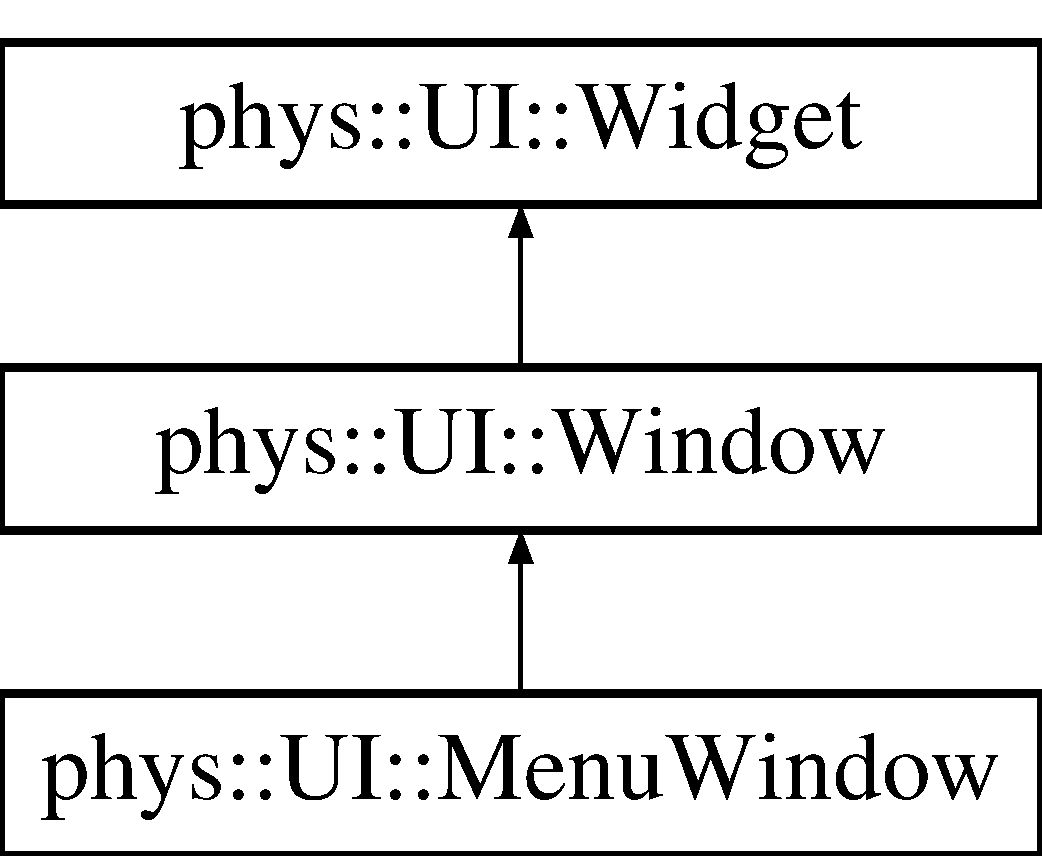
\includegraphics[height=3.000000cm]{classphys_1_1UI_1_1Window}
\end{center}
\end{figure}
\subsubsection*{Public Member Functions}
\begin{DoxyCompactItemize}
\item 
virtual bool \hyperlink{classphys_1_1UI_1_1Window_a771bc9e43c0492ab179d8126c30665cf}{CheckMouseHover} ()
\begin{DoxyCompactList}\small\item\em Checks to see if the current mouse position is over this window. \item\end{DoxyCompactList}\item 
virtual \hyperlink{classphys_1_1UI_1_1Button}{Button} $\ast$ \hyperlink{classphys_1_1UI_1_1Window_add2be540cd01477a93d0e6362bc4de1f}{CreateButton} (\hyperlink{namespacephys_a5ce5049f8b4bf88d6413c47b504ebb31}{ConstString} \&Name, const \hyperlink{structphys_1_1UI_1_1RenderableRect}{RenderableRect} \&Rect)
\begin{DoxyCompactList}\small\item\em Creates a button within this \hyperlink{classphys_1_1UI_1_1Window}{Window}. \item\end{DoxyCompactList}\item 
virtual \hyperlink{classphys_1_1UI_1_1ButtonListBox}{UI::ButtonListBox} $\ast$ \hyperlink{classphys_1_1UI_1_1Window_addeb37ade50e251e9209afdaab952bc7}{CreateButtonListBox} (\hyperlink{namespacephys_a5ce5049f8b4bf88d6413c47b504ebb31}{ConstString} \&Name, const \hyperlink{structphys_1_1UI_1_1RenderableRect}{RenderableRect} \&Rect, const \hyperlink{namespacephys_af7eb897198d265b8e868f45240230d5f}{Real} \&ScrollbarWidth, const UI::ScrollbarStyle \&ScrollbarStyle)
\begin{DoxyCompactList}\small\item\em Creates a \hyperlink{classphys_1_1UI_1_1Button}{Button} List Box within this \hyperlink{classphys_1_1UI_1_1Window}{Window}. \item\end{DoxyCompactList}\item 
virtual \hyperlink{classphys_1_1UI_1_1Caption}{Caption} $\ast$ \hyperlink{classphys_1_1UI_1_1Window_a0116b152891c33e91e6385cf6a2df40c}{CreateCaption} (\hyperlink{namespacephys_a5ce5049f8b4bf88d6413c47b504ebb31}{ConstString} \&Name, const \hyperlink{structphys_1_1UI_1_1RenderableRect}{RenderableRect} \&Rect, const \hyperlink{namespacephys_a460f6bc24c8dd347b05e0366ae34f34a}{Whole} \&Glyph, const \hyperlink{namespacephys_aa03900411993de7fbfec4789bc1d392e}{String} \&Text)
\begin{DoxyCompactList}\small\item\em Creates a caption within this \hyperlink{classphys_1_1UI_1_1Window}{Window}. \item\end{DoxyCompactList}\item 
virtual \hyperlink{classphys_1_1UI_1_1Caption}{Caption} $\ast$ \hyperlink{classphys_1_1UI_1_1Window_a2a461f25fe555f8f249697f0afdd983c}{CreateCaption} (\hyperlink{namespacephys_a5ce5049f8b4bf88d6413c47b504ebb31}{ConstString} \&Name, const \hyperlink{structphys_1_1UI_1_1RenderableRect}{RenderableRect} \&Rect, const \hyperlink{namespacephys_af7eb897198d265b8e868f45240230d5f}{Real} \&LineHeight, const \hyperlink{namespacephys_aa03900411993de7fbfec4789bc1d392e}{String} \&Text)
\begin{DoxyCompactList}\small\item\em Creates a caption within this layer. \item\end{DoxyCompactList}\item 
virtual \hyperlink{classphys_1_1UI_1_1CheckBox}{UI::CheckBox} $\ast$ \hyperlink{classphys_1_1UI_1_1Window_aa1bab1d930293e01ca8af34dc6e3d2e4}{CreateCheckBox} (\hyperlink{namespacephys_a5ce5049f8b4bf88d6413c47b504ebb31}{ConstString} \&Name, const \hyperlink{structphys_1_1UI_1_1RenderableRect}{RenderableRect} \&Rect, const \hyperlink{namespacephys_a460f6bc24c8dd347b05e0366ae34f34a}{Whole} \&Glyph, const \hyperlink{namespacephys_aa03900411993de7fbfec4789bc1d392e}{String} \&LabelText)
\begin{DoxyCompactList}\small\item\em Creates a \hyperlink{classphys_1_1UI_1_1CheckBox}{CheckBox} within this \hyperlink{classphys_1_1UI_1_1Window}{Window}. \item\end{DoxyCompactList}\item 
virtual \hyperlink{classphys_1_1UI_1_1ListBox}{UI::ListBox} $\ast$ \hyperlink{classphys_1_1UI_1_1Window_ade0d2d18173849e4836badbf216343fc}{CreateListBox} (\hyperlink{namespacephys_a5ce5049f8b4bf88d6413c47b504ebb31}{ConstString} \&Name, const \hyperlink{structphys_1_1UI_1_1RenderableRect}{RenderableRect} \&Rect, const UI::ScrollbarStyle \&ScrollbarStyle)
\begin{DoxyCompactList}\small\item\em Creates a List Box within this \hyperlink{classphys_1_1UI_1_1Window}{Window}. \item\end{DoxyCompactList}\item 
virtual \hyperlink{classphys_1_1UI_1_1MarkupText}{MarkupText} $\ast$ \hyperlink{classphys_1_1UI_1_1Window_a048621c7d504f9bf75d68e62a7384849}{CreateMarkupText} (\hyperlink{namespacephys_a5ce5049f8b4bf88d6413c47b504ebb31}{ConstString} \&Name, const \hyperlink{structphys_1_1UI_1_1RenderableRect}{RenderableRect} \&Rect, const \hyperlink{namespacephys_a460f6bc24c8dd347b05e0366ae34f34a}{Whole} \&Glyph, const \hyperlink{namespacephys_aa03900411993de7fbfec4789bc1d392e}{String} \&Text)
\begin{DoxyCompactList}\small\item\em Creates a markup text within this \hyperlink{classphys_1_1UI_1_1Window}{Window}. \item\end{DoxyCompactList}\item 
virtual \hyperlink{classphys_1_1UI_1_1MarkupText}{MarkupText} $\ast$ \hyperlink{classphys_1_1UI_1_1Window_ab8281178ff1eb69653267da24c91999b}{CreateMarkupText} (\hyperlink{namespacephys_a5ce5049f8b4bf88d6413c47b504ebb31}{ConstString} \&Name, const \hyperlink{structphys_1_1UI_1_1RenderableRect}{RenderableRect} \&Rect, const \hyperlink{namespacephys_af7eb897198d265b8e868f45240230d5f}{Real} \&LineHeight, const \hyperlink{namespacephys_aa03900411993de7fbfec4789bc1d392e}{String} \&Text)
\begin{DoxyCompactList}\small\item\em Creates a markup text within this layer. \item\end{DoxyCompactList}\item 
virtual \hyperlink{classphys_1_1UI_1_1PagedCellGrid}{UI::PagedCellGrid} $\ast$ \hyperlink{classphys_1_1UI_1_1Window_a8d38e4d364a3b25731e4fba4032f0acf}{CreatePagedCellGrid} (\hyperlink{namespacephys_a5ce5049f8b4bf88d6413c47b504ebb31}{ConstString} \&Name, const \hyperlink{structphys_1_1UI_1_1RenderableRect}{RenderableRect} \&Rect, const \hyperlink{structphys_1_1UI_1_1RenderableRect}{RenderableRect} \&SpnRect, const UI::SpinnerStyle \&SStyle, const \hyperlink{namespacephys_af7eb897198d265b8e868f45240230d5f}{Real} \&GlyphHeight)
\begin{DoxyCompactList}\small\item\em Creates a paged cell grid within this layer. \item\end{DoxyCompactList}\item 
virtual \hyperlink{classphys_1_1UI_1_1Rectangle}{Rectangle} $\ast$ \hyperlink{classphys_1_1UI_1_1Window_a6388ff0085a5bf40942c4b21b1b0e141}{CreateRectangle} (const \hyperlink{structphys_1_1UI_1_1RenderableRect}{RenderableRect} \&Rect)
\begin{DoxyCompactList}\small\item\em Creates a rectangle within this \hyperlink{classphys_1_1UI_1_1Window}{Window}. \item\end{DoxyCompactList}\item 
virtual \hyperlink{classphys_1_1UI_1_1Scrollbar}{UI::Scrollbar} $\ast$ \hyperlink{classphys_1_1UI_1_1Window_af25f6535f3a785f779df43a7f01845e0}{CreateScrollbar} (\hyperlink{namespacephys_a5ce5049f8b4bf88d6413c47b504ebb31}{ConstString} \&Name, const \hyperlink{structphys_1_1UI_1_1RenderableRect}{RenderableRect} \&Rect, const UI::ScrollbarStyle \&Style)
\begin{DoxyCompactList}\small\item\em Creates a \hyperlink{classphys_1_1UI_1_1Scrollbar}{Scrollbar} within this \hyperlink{classphys_1_1UI_1_1Window}{Window}. \item\end{DoxyCompactList}\item 
virtual \hyperlink{classphys_1_1UI_1_1ScrolledCellGrid}{UI::ScrolledCellGrid} $\ast$ \hyperlink{classphys_1_1UI_1_1Window_ade46bf7aae0302d8b2d44a4513eb0915}{CreateScrolledCellGrid} (\hyperlink{namespacephys_a5ce5049f8b4bf88d6413c47b504ebb31}{ConstString} \&Name, const \hyperlink{structphys_1_1UI_1_1RenderableRect}{RenderableRect} \&Rect, const \hyperlink{namespacephys_af7eb897198d265b8e868f45240230d5f}{Real} \&Thickness, const UI::ScrollbarStyle \&Style)
\begin{DoxyCompactList}\small\item\em Creates a scrolled cell grid within this layer. \item\end{DoxyCompactList}\item 
virtual \hyperlink{classphys_1_1UI_1_1Spinner}{UI::Spinner} $\ast$ \hyperlink{classphys_1_1UI_1_1Window_a9f08d5531890927980483448226d7656}{CreateSpinner} (\hyperlink{namespacephys_a5ce5049f8b4bf88d6413c47b504ebb31}{ConstString} \&Name, const \hyperlink{structphys_1_1UI_1_1RenderableRect}{RenderableRect} \&Rect, const UI::SpinnerStyle \&SStyle, const \hyperlink{namespacephys_af7eb897198d265b8e868f45240230d5f}{Real} \&GlyphHeight)
\begin{DoxyCompactList}\small\item\em Creates a \hyperlink{classphys_1_1UI_1_1Spinner}{Spinner} within this layer. \item\end{DoxyCompactList}\item 
virtual \hyperlink{classphys_1_1UI_1_1TextButton}{TextButton} $\ast$ \hyperlink{classphys_1_1UI_1_1Window_abcc01b8fb17ba93c87a46b746350913e}{CreateTextButton} (\hyperlink{namespacephys_a5ce5049f8b4bf88d6413c47b504ebb31}{ConstString} \&Name, const \hyperlink{structphys_1_1UI_1_1RenderableRect}{RenderableRect} \&Rect, const \hyperlink{namespacephys_a460f6bc24c8dd347b05e0366ae34f34a}{Whole} \&Glyph, \hyperlink{namespacephys_a5ce5049f8b4bf88d6413c47b504ebb31}{ConstString} \&Text)
\begin{DoxyCompactList}\small\item\em Creates a text button within this \hyperlink{classphys_1_1UI_1_1Window}{Window}. \item\end{DoxyCompactList}\item 
virtual \hyperlink{classphys_1_1UI_1_1TextButton}{TextButton} $\ast$ \hyperlink{classphys_1_1UI_1_1Window_aafdd954c57021628d8f96a56e0b06346}{CreateTextButton} (\hyperlink{namespacephys_a5ce5049f8b4bf88d6413c47b504ebb31}{ConstString} \&Name, const \hyperlink{structphys_1_1UI_1_1RenderableRect}{RenderableRect} \&Rect, const \hyperlink{namespacephys_af7eb897198d265b8e868f45240230d5f}{Real} \&LineHeight, \hyperlink{namespacephys_a5ce5049f8b4bf88d6413c47b504ebb31}{ConstString} \&Text)
\begin{DoxyCompactList}\small\item\em Creates a text button within this layer. \item\end{DoxyCompactList}\item 
void \hyperlink{classphys_1_1UI_1_1Window_a5a5bc10054d6e1d709b3b683a5554bf4}{DestroyButton} (\hyperlink{classphys_1_1UI_1_1Button}{UI::Button} $\ast$ToBeDestroyed)
\begin{DoxyCompactList}\small\item\em Destroys a button. \item\end{DoxyCompactList}\item 
virtual void \hyperlink{classphys_1_1UI_1_1Window_a4e3dbe56ca1efce7ac1d26ceb8f7e915}{DestroyCaption} (\hyperlink{classphys_1_1UI_1_1Caption}{UI::Caption} $\ast$ToBeDestroyed)
\begin{DoxyCompactList}\small\item\em Destroys a caption. \item\end{DoxyCompactList}\item 
virtual void \hyperlink{classphys_1_1UI_1_1Window_aba2506738c7cccfbf8297bf03e431cb8}{DestroyMarkupText} (\hyperlink{classphys_1_1UI_1_1MarkupText}{UI::MarkupText} $\ast$ToBeDestroyed)
\begin{DoxyCompactList}\small\item\em Destroys a markup text. \item\end{DoxyCompactList}\item 
virtual void \hyperlink{classphys_1_1UI_1_1Window_ab66c4c1d5f26e3f4fcdd34063b711365}{DestroyRectangle} (\hyperlink{classphys_1_1UI_1_1Rectangle}{UI::Rectangle} $\ast$ToBeDestroyed)
\begin{DoxyCompactList}\small\item\em Destroys a rectangle. \item\end{DoxyCompactList}\item 
virtual void \hyperlink{classphys_1_1UI_1_1Window_ab4bda54a82b64aec2cf4e03201a40772}{DestroyWidget} (\hyperlink{classphys_1_1UI_1_1Widget}{UI::Widget} $\ast$ToBeDestroyed)
\begin{DoxyCompactList}\small\item\em Destroys a widget. \item\end{DoxyCompactList}\item 
virtual \hyperlink{classphys_1_1Vector2}{Vector2} \hyperlink{classphys_1_1UI_1_1Window_a811fb495bc698752e03778b18f2b1a30}{GetActualPosition} ()
\begin{DoxyCompactList}\small\item\em Sets the pixel position of this window. \item\end{DoxyCompactList}\item 
virtual \hyperlink{classphys_1_1Vector2}{Vector2} \hyperlink{classphys_1_1UI_1_1Window_a22f5ca800e44c5e2cfeed59c243b03ed}{GetActualSize} ()
\begin{DoxyCompactList}\small\item\em Sets the pixel size of this window. \item\end{DoxyCompactList}\item 
virtual \hyperlink{classphys_1_1UI_1_1Button}{Button} $\ast$ \hyperlink{classphys_1_1UI_1_1Window_ab1152992cf6b636c8a4911889d930d9a}{GetButton} (\hyperlink{namespacephys_a5ce5049f8b4bf88d6413c47b504ebb31}{ConstString} \&Name)
\begin{DoxyCompactList}\small\item\em Gets an already created button by name. \item\end{DoxyCompactList}\item 
virtual \hyperlink{classphys_1_1UI_1_1Button}{Button} $\ast$ \hyperlink{classphys_1_1UI_1_1Window_aa0fb8f15e5a0ee2ac46631f56e23fa36}{GetButton} (const \hyperlink{namespacephys_a460f6bc24c8dd347b05e0366ae34f34a}{Whole} \&Index)
\begin{DoxyCompactList}\small\item\em Gets an already created button by index. \item\end{DoxyCompactList}\item 
virtual \hyperlink{classphys_1_1UI_1_1Caption}{Caption} $\ast$ \hyperlink{classphys_1_1UI_1_1Window_acfc2669ecac2824bfa7cc53eb724d191}{GetCaption} (\hyperlink{namespacephys_a5ce5049f8b4bf88d6413c47b504ebb31}{ConstString} \&Name)
\begin{DoxyCompactList}\small\item\em Gets an already created caption by name. \item\end{DoxyCompactList}\item 
virtual \hyperlink{classphys_1_1UI_1_1Caption}{Caption} $\ast$ \hyperlink{classphys_1_1UI_1_1Window_a658864b36968fce9ab09f3d5cb14b21a}{GetCaption} (const \hyperlink{namespacephys_a460f6bc24c8dd347b05e0366ae34f34a}{Whole} \&Index)
\begin{DoxyCompactList}\small\item\em Gets an already created caption by index. \item\end{DoxyCompactList}\item 
virtual \hyperlink{classphys_1_1UI_1_1MarkupText}{MarkupText} $\ast$ \hyperlink{classphys_1_1UI_1_1Window_af5bf2246915fc68558d2a68ed016a68b}{GetMarkupText} (\hyperlink{namespacephys_a5ce5049f8b4bf88d6413c47b504ebb31}{ConstString} \&Name)
\begin{DoxyCompactList}\small\item\em Gets an already created markup text by name. \item\end{DoxyCompactList}\item 
virtual \hyperlink{classphys_1_1UI_1_1MarkupText}{MarkupText} $\ast$ \hyperlink{classphys_1_1UI_1_1Window_a7f9a97e3f8c70b0a7917a7768e5d53aa}{GetMarkupText} (const \hyperlink{namespacephys_a460f6bc24c8dd347b05e0366ae34f34a}{Whole} \&Index)
\begin{DoxyCompactList}\small\item\em Gets an already created markup text by index. \item\end{DoxyCompactList}\item 
virtual \hyperlink{namespacephys_a460f6bc24c8dd347b05e0366ae34f34a}{Whole} \hyperlink{classphys_1_1UI_1_1Window_a7eab9b4e1607a2b796072f60b6e3e0cd}{GetNumButtons} ()
\begin{DoxyCompactList}\small\item\em Gets the number of buttons created and stored in this class. \item\end{DoxyCompactList}\item 
virtual \hyperlink{namespacephys_a460f6bc24c8dd347b05e0366ae34f34a}{Whole} \hyperlink{classphys_1_1UI_1_1Window_a125d78e98b47a4d93f6414545fd2374c}{GetNumCaptions} ()
\begin{DoxyCompactList}\small\item\em Gets the number of captions created and stored in this class. \item\end{DoxyCompactList}\item 
virtual \hyperlink{namespacephys_a460f6bc24c8dd347b05e0366ae34f34a}{Whole} \hyperlink{classphys_1_1UI_1_1Window_ac9e23e41ffff8ef475fcdb0c25bad240}{GetNumMarkupTexts} ()
\begin{DoxyCompactList}\small\item\em Gets the number of markup texts created and stored in this class. \item\end{DoxyCompactList}\item 
virtual \hyperlink{namespacephys_a460f6bc24c8dd347b05e0366ae34f34a}{Whole} \hyperlink{classphys_1_1UI_1_1Window_a4d2d8821df32a920e7389b37f50f7c6d}{GetNumRectangles} ()
\begin{DoxyCompactList}\small\item\em Gets the number of rectangles created and stored in this class. \item\end{DoxyCompactList}\item 
virtual \hyperlink{namespacephys_a460f6bc24c8dd347b05e0366ae34f34a}{Whole} \hyperlink{classphys_1_1UI_1_1Window_a062270984d25dca44f0bc4d65ef324a0}{GetNumWidgets} ()
\begin{DoxyCompactList}\small\item\em Gets the number of widgets created and stored in this class. \item\end{DoxyCompactList}\item 
virtual \hyperlink{structphys_1_1UI_1_1ResizingInfo}{OffsetButtonInfo} $\ast$ \hyperlink{classphys_1_1UI_1_1Window_ad0d6b12c2f69ea1bc580bba7e69949a5}{GetOffsetButtonInfo} (\hyperlink{namespacephys_a5ce5049f8b4bf88d6413c47b504ebb31}{ConstString} \&Name)
\begin{DoxyCompactList}\small\item\em Gets the OffsetButtonInfo of an already created button by name. \item\end{DoxyCompactList}\item 
virtual \hyperlink{structphys_1_1UI_1_1ResizingInfo}{OffsetButtonInfo} $\ast$ \hyperlink{classphys_1_1UI_1_1Window_a965b9fbfa8fa73b351f468a65ca73dcc}{GetOffsetButtonInfo} (const \hyperlink{namespacephys_a460f6bc24c8dd347b05e0366ae34f34a}{Whole} \&Index)
\begin{DoxyCompactList}\small\item\em Gets the OffsetButtonInfo of an already created button by index. \item\end{DoxyCompactList}\item 
virtual \hyperlink{structphys_1_1UI_1_1ResizingInfo}{OffsetCaptionInfo} $\ast$ \hyperlink{classphys_1_1UI_1_1Window_a64dc0b65518151f3f36bb4ad40505804}{GetOffsetCaptionInfo} (const \hyperlink{namespacephys_a460f6bc24c8dd347b05e0366ae34f34a}{Whole} \&Index)
\begin{DoxyCompactList}\small\item\em Gets the OffsetCaptionInfo of an already created caption by index. \item\end{DoxyCompactList}\item 
virtual \hyperlink{structphys_1_1UI_1_1ResizingInfo}{OffsetCaptionInfo} $\ast$ \hyperlink{classphys_1_1UI_1_1Window_afa081532c017f5e8c4f04bfd2df207b6}{GetOffsetCaptionInfo} (\hyperlink{namespacephys_a5ce5049f8b4bf88d6413c47b504ebb31}{ConstString} \&Name)
\begin{DoxyCompactList}\small\item\em Gets the OffsetCaptionInfo of an already created caption by name. \item\end{DoxyCompactList}\item 
virtual \hyperlink{structphys_1_1UI_1_1ResizingInfo}{OffsetMarkupTextInfo} $\ast$ \hyperlink{classphys_1_1UI_1_1Window_a9906bb131f631af0a9aed7dbb7744112}{GetOffsetMarkupTextInfo} (\hyperlink{namespacephys_a5ce5049f8b4bf88d6413c47b504ebb31}{ConstString} \&Name)
\begin{DoxyCompactList}\small\item\em Gets the OffsetMarkupTextInfo of an already created markup text by name. \item\end{DoxyCompactList}\item 
virtual \hyperlink{structphys_1_1UI_1_1ResizingInfo}{OffsetMarkupTextInfo} $\ast$ \hyperlink{classphys_1_1UI_1_1Window_aa809c88016b239c81b53e060b547ec85}{GetOffsetMarkupTextInfo} (const \hyperlink{namespacephys_a460f6bc24c8dd347b05e0366ae34f34a}{Whole} \&Index)
\begin{DoxyCompactList}\small\item\em Gets the OffsetMarkupTextInfo of an already created markup text by index. \item\end{DoxyCompactList}\item 
virtual \hyperlink{structphys_1_1UI_1_1ResizingInfo}{OffsetRectangleInfo} $\ast$ \hyperlink{classphys_1_1UI_1_1Window_ae8593fa6cd22ed15dd0b0daf9dcb69d3}{GetOffsetRectangleInfo} (const \hyperlink{namespacephys_a460f6bc24c8dd347b05e0366ae34f34a}{Whole} \&Index)
\begin{DoxyCompactList}\small\item\em Gets the OffsetRectangleInfo of an already created rectangle by index. \item\end{DoxyCompactList}\item 
virtual \hyperlink{structphys_1_1UI_1_1ResizingInfo}{OffsetWidgetInfo} $\ast$ \hyperlink{classphys_1_1UI_1_1Window_a77a2091e41766344253cac55af650f54}{GetOffsetWidgetInfo} (\hyperlink{namespacephys_a5ce5049f8b4bf88d6413c47b504ebb31}{ConstString} \&Name)
\begin{DoxyCompactList}\small\item\em Gets the OffsetWidgetInfo of an already created widget by name. \item\end{DoxyCompactList}\item 
virtual \hyperlink{structphys_1_1UI_1_1ResizingInfo}{OffsetWidgetInfo} $\ast$ \hyperlink{classphys_1_1UI_1_1Window_aa3691702f83c0369c4e5b1cec317e656}{GetOffsetWidgetInfo} (const \hyperlink{namespacephys_a460f6bc24c8dd347b05e0366ae34f34a}{Whole} \&Index)
\begin{DoxyCompactList}\small\item\em Gets the OffsetWidgetInfo of an already created widget by index. \item\end{DoxyCompactList}\item 
virtual \hyperlink{classphys_1_1Vector2}{Vector2} \hyperlink{classphys_1_1UI_1_1Window_a29fca96d9a2dab29d77a36d6a329f306}{GetPosition} ()
\begin{DoxyCompactList}\small\item\em Gets the relative position of this window. \item\end{DoxyCompactList}\item 
virtual \hyperlink{classphys_1_1UI_1_1Rectangle}{Rectangle} $\ast$ \hyperlink{classphys_1_1UI_1_1Window_a522a0af5999c8fae7009e09752b1a430}{GetRectangle} (const \hyperlink{namespacephys_a460f6bc24c8dd347b05e0366ae34f34a}{Whole} \&Index)
\begin{DoxyCompactList}\small\item\em Gets an already created rectangle by index. \item\end{DoxyCompactList}\item 
virtual \hyperlink{classphys_1_1Vector2}{Vector2} \hyperlink{classphys_1_1UI_1_1Window_a9946100eb6e6e985921bbea9e87cede3}{GetSize} ()
\begin{DoxyCompactList}\small\item\em Gets the relative size of this window. \item\end{DoxyCompactList}\item 
virtual \hyperlink{classphys_1_1UI_1_1Widget}{Widget} $\ast$ \hyperlink{classphys_1_1UI_1_1Window_a0d2274afdabda9915d242dc3d057ae61}{GetWidget} (\hyperlink{namespacephys_a5ce5049f8b4bf88d6413c47b504ebb31}{ConstString} \&Name)
\begin{DoxyCompactList}\small\item\em Gets an already created widget by name. \item\end{DoxyCompactList}\item 
virtual \hyperlink{classphys_1_1UI_1_1Widget}{Widget} $\ast$ \hyperlink{classphys_1_1UI_1_1Window_ab70e34505b0cfbdfe8fa5df9748238df}{GetWidget} (const \hyperlink{namespacephys_a460f6bc24c8dd347b05e0366ae34f34a}{Whole} \&Index)
\begin{DoxyCompactList}\small\item\em Gets an already created widget by index. \item\end{DoxyCompactList}\item 
virtual \hyperlink{classphys_1_1UI_1_1Rectangle}{Rectangle} $\ast$ \hyperlink{classphys_1_1UI_1_1Window_af06ae5666145e4d8835b38f4a9cbca2a}{GetWindowBack} ()
\begin{DoxyCompactList}\small\item\em Gets the background object of this window. \item\end{DoxyCompactList}\item 
\hypertarget{classphys_1_1UI_1_1Window_a5eb51c6e1b2c440b52196fcf1022285e}{
virtual void \hyperlink{classphys_1_1UI_1_1Window_a5eb51c6e1b2c440b52196fcf1022285e}{Hide} ()}
\label{classphys_1_1UI_1_1Window_a5eb51c6e1b2c440b52196fcf1022285e}

\begin{DoxyCompactList}\small\item\em Forces this window to hide. \item\end{DoxyCompactList}\item 
virtual bool \hyperlink{classphys_1_1UI_1_1Window_aa1d88c50c0965510b494b51f3e5a7bf0}{IsVisible} ()
\begin{DoxyCompactList}\small\item\em Gets the visibility of this window. \item\end{DoxyCompactList}\item 
virtual void \hyperlink{classphys_1_1UI_1_1Window_a45a3d0454803ce26a053f645b965d16b}{SetActualPosition} (const \hyperlink{classphys_1_1Vector2}{Vector2} \&Position)
\begin{DoxyCompactList}\small\item\em Sets the pixel position of this window. \item\end{DoxyCompactList}\item 
virtual void \hyperlink{classphys_1_1UI_1_1Window_a002150cd8db87283bead5f10b2310152}{SetActualSize} (const \hyperlink{classphys_1_1Vector2}{Vector2} \&Size)
\begin{DoxyCompactList}\small\item\em Sets the pixel size of this window. \item\end{DoxyCompactList}\item 
virtual void \hyperlink{classphys_1_1UI_1_1Window_a17e6284d4ac5aa95f257c5168d6cc5ac}{SetPosition} (const \hyperlink{classphys_1_1Vector2}{Vector2} \&Position)
\begin{DoxyCompactList}\small\item\em Sets the relative position of this window. \item\end{DoxyCompactList}\item 
virtual void \hyperlink{classphys_1_1UI_1_1Window_a88ed4d21758cee9afeadc4069c3e0b04}{SetSize} (const \hyperlink{classphys_1_1Vector2}{Vector2} \&Size)
\begin{DoxyCompactList}\small\item\em Sets the relative size of this window. \item\end{DoxyCompactList}\item 
virtual void \hyperlink{classphys_1_1UI_1_1Window_a351439e78013bc87ecadcc00bce08573}{SetVisible} (bool visible)
\begin{DoxyCompactList}\small\item\em Sets the visibility of this window. \item\end{DoxyCompactList}\item 
\hypertarget{classphys_1_1UI_1_1Window_af945bd84876d577d1dc6e1c7e28329a8}{
virtual void \hyperlink{classphys_1_1UI_1_1Window_af945bd84876d577d1dc6e1c7e28329a8}{Show} ()}
\label{classphys_1_1UI_1_1Window_af945bd84876d577d1dc6e1c7e28329a8}

\begin{DoxyCompactList}\small\item\em Forces this window to be shown. \item\end{DoxyCompactList}\item 
virtual void \hyperlink{classphys_1_1UI_1_1Window_a0be6c93e5660757a5f94227f2e076ba9}{UpdateDimensions} (const \hyperlink{classphys_1_1Vector2}{Vector2} \&OldViewportSize)
\begin{DoxyCompactList}\small\item\em Updates the dimensions of this widget to match those of the new screen size. \item\end{DoxyCompactList}\item 
\hyperlink{classphys_1_1UI_1_1Window_a2a85e34ec05ddf8e2713c02b5d6e7c90}{Window} (\hyperlink{namespacephys_a5ce5049f8b4bf88d6413c47b504ebb31}{ConstString} \&name, const \hyperlink{structphys_1_1UI_1_1RenderableRect}{RenderableRect} \&Rect, \hyperlink{classphys_1_1UI_1_1Layer}{Layer} $\ast$PLayer)
\begin{DoxyCompactList}\small\item\em Standard initialization constructor. \item\end{DoxyCompactList}\item 
\hypertarget{classphys_1_1UI_1_1Window_a3480249de9950a3993c5e7f836aa8f59}{
virtual \hyperlink{classphys_1_1UI_1_1Window_a3480249de9950a3993c5e7f836aa8f59}{$\sim$Window} ()}
\label{classphys_1_1UI_1_1Window_a3480249de9950a3993c5e7f836aa8f59}

\begin{DoxyCompactList}\small\item\em Standard destructor. \item\end{DoxyCompactList}\end{DoxyCompactItemize}
\subsubsection*{Protected Types}
\begin{DoxyCompactItemize}
\item 
enum \hyperlink{classphys_1_1UI_1_1Window_ab7ecb300d312f54556615d3a3b8c6dc9}{ResizeMode} \{ \par
{\bfseries RM\_\-None}, 
{\bfseries RM\_\-TopLeft}, 
{\bfseries RM\_\-TopRight}, 
{\bfseries RM\_\-BottomLeft}, 
\par
{\bfseries RM\_\-BottomRight}, 
{\bfseries RM\_\-Left}, 
{\bfseries RM\_\-Right}, 
{\bfseries RM\_\-Top}, 
\par
{\bfseries RM\_\-Bottom}
 \}
\begin{DoxyCompactList}\small\item\em Internal enum for handling a resizing via mouse. \item\end{DoxyCompactList}\end{DoxyCompactItemize}
\subsubsection*{Protected Member Functions}
\begin{DoxyCompactItemize}
\item 
\hypertarget{classphys_1_1UI_1_1Window_ad9b1048dac8e30d5a87393e561f0ab4a}{
void \hyperlink{classphys_1_1UI_1_1Window_ad9b1048dac8e30d5a87393e561f0ab4a}{BorderAreaCheck} (const \hyperlink{classphys_1_1Vector2}{Vector2} \&ScreenLoc)}
\label{classphys_1_1UI_1_1Window_ad9b1048dac8e30d5a87393e561f0ab4a}

\begin{DoxyCompactList}\small\item\em Checks to see if a point is within the border of this window. \item\end{DoxyCompactList}\item 
\hypertarget{classphys_1_1UI_1_1Window_ae733d9dc3b0bc37c91dc7002c8b01bc7}{
\hyperlink{classphys_1_1Vector2}{Vector2} \hyperlink{classphys_1_1UI_1_1Window_ae733d9dc3b0bc37c91dc7002c8b01bc7}{CalculateOffset} (const \hyperlink{classphys_1_1Vector2}{Vector2} NewSize, const \hyperlink{classphys_1_1Vector2}{Vector2} OldSize, const \hyperlink{classphys_1_1Vector2}{Vector2} EleOffset, UI::ResizeableAnchor Anchor)}
\label{classphys_1_1UI_1_1Window_ae733d9dc3b0bc37c91dc7002c8b01bc7}

\begin{DoxyCompactList}\small\item\em Calculates a new offset for an individual element. \item\end{DoxyCompactList}\item 
\hypertarget{classphys_1_1UI_1_1Window_a4d120ac244f9a9c683f8b9bdb90835a8}{
\hyperlink{classphys_1_1Vector2}{Vector2} \hyperlink{classphys_1_1UI_1_1Window_a4d120ac244f9a9c683f8b9bdb90835a8}{CalculateSize} (const \hyperlink{classphys_1_1Vector2}{Vector2} NewSize, const \hyperlink{classphys_1_1Vector2}{Vector2} OldSize, const \hyperlink{classphys_1_1Vector2}{Vector2} EleSize, UI::ResizeableTether Tether)}
\label{classphys_1_1UI_1_1Window_a4d120ac244f9a9c683f8b9bdb90835a8}

\begin{DoxyCompactList}\small\item\em Calculates a new size for an individual element. \item\end{DoxyCompactList}\item 
\hypertarget{classphys_1_1UI_1_1Window_ab0917b15904f30d66e6ef81b840601e2}{
void \hyperlink{classphys_1_1UI_1_1Window_ab0917b15904f30d66e6ef81b840601e2}{SetArea} (const \hyperlink{classphys_1_1Vector2}{Vector2} \&Size)}
\label{classphys_1_1UI_1_1Window_ab0917b15904f30d66e6ef81b840601e2}

\begin{DoxyCompactList}\small\item\em Internal function for setting the area(size) of this widget. \item\end{DoxyCompactList}\item 
\hypertarget{classphys_1_1UI_1_1Window_a72f45126d1a8282f03054470c94218bf}{
void \hyperlink{classphys_1_1UI_1_1Window_a72f45126d1a8282f03054470c94218bf}{SetLocation} (const \hyperlink{classphys_1_1Vector2}{Vector2} \&Position)}
\label{classphys_1_1UI_1_1Window_a72f45126d1a8282f03054470c94218bf}

\begin{DoxyCompactList}\small\item\em Internal function for setting the location(position) of this widget. \item\end{DoxyCompactList}\item 
\hypertarget{classphys_1_1UI_1_1Window_a867bbe36b9eb74e9fb306303258be5a4}{
void \hyperlink{classphys_1_1UI_1_1Window_a867bbe36b9eb74e9fb306303258be5a4}{Update} (bool Force=false)}
\label{classphys_1_1UI_1_1Window_a867bbe36b9eb74e9fb306303258be5a4}

\begin{DoxyCompactList}\small\item\em For use with widget update/automation. \item\end{DoxyCompactList}\end{DoxyCompactItemize}
\subsubsection*{Protected Attributes}
\begin{DoxyCompactItemize}
\item 
\hypertarget{classphys_1_1UI_1_1Window_af686c8e14e1a19b68cfb3332cc94c7b7}{
\hyperlink{namespacephys_a460f6bc24c8dd347b05e0366ae34f34a}{Whole} {\bfseries BorderWidth}}
\label{classphys_1_1UI_1_1Window_af686c8e14e1a19b68cfb3332cc94c7b7}

\item 
\hypertarget{classphys_1_1UI_1_1Window_a5fccbc2f8975e9a60b4b7c6d5eca4844}{
std::vector$<$ \hyperlink{structphys_1_1UI_1_1ResizingInfo}{OffsetButtonInfo} $>$ {\bfseries Buttons}}
\label{classphys_1_1UI_1_1Window_a5fccbc2f8975e9a60b4b7c6d5eca4844}

\item 
\hypertarget{classphys_1_1UI_1_1Window_acaa4a2954c71b6a9ea6edb1941ca053d}{
std::vector$<$ \hyperlink{structphys_1_1UI_1_1ResizingInfo}{OffsetCaptionInfo} $>$ {\bfseries Captions}}
\label{classphys_1_1UI_1_1Window_acaa4a2954c71b6a9ea6edb1941ca053d}

\item 
\hypertarget{classphys_1_1UI_1_1Window_acde8d004d5ac67b969fbd66b35f818fa}{
\hyperlink{classphys_1_1UI_1_1Window_ab7ecb300d312f54556615d3a3b8c6dc9}{ResizeMode} {\bfseries CurrentRM}}
\label{classphys_1_1UI_1_1Window_acde8d004d5ac67b969fbd66b35f818fa}

\item 
\hypertarget{classphys_1_1UI_1_1Window_ac50afa68d42e2f30ea5d470b03be4786}{
std::vector$<$ \hyperlink{structphys_1_1UI_1_1ResizingInfo}{OffsetMarkupTextInfo} $>$ {\bfseries MarkupTexts}}
\label{classphys_1_1UI_1_1Window_ac50afa68d42e2f30ea5d470b03be4786}

\item 
\hypertarget{classphys_1_1UI_1_1Window_a556a43730021df62a867af76a03069b0}{
std::vector$<$ \hyperlink{structphys_1_1UI_1_1ResizingInfo}{OffsetRectangleInfo} $>$ {\bfseries Rectangles}}
\label{classphys_1_1UI_1_1Window_a556a43730021df62a867af76a03069b0}

\item 
\hypertarget{classphys_1_1UI_1_1Window_a2fc4fb5f39925eff948c8cb61f9a724f}{
std::vector$<$ \hyperlink{structphys_1_1UI_1_1ResizingInfo}{OffsetWidgetInfo} $>$ {\bfseries Widgets}}
\label{classphys_1_1UI_1_1Window_a2fc4fb5f39925eff948c8cb61f9a724f}

\item 
\hypertarget{classphys_1_1UI_1_1Window_a91635b1e1a94e74e76ebfe61611d1daf}{
\hyperlink{classphys_1_1UI_1_1Rectangle}{Rectangle} $\ast$ {\bfseries WindowBack}}
\label{classphys_1_1UI_1_1Window_a91635b1e1a94e74e76ebfe61611d1daf}

\end{DoxyCompactItemize}


\subsubsection{Detailed Description}
This is a container widget capable of holding any other widget. 

Definition at line 76 of file uiwindow.h.



\subsubsection{Constructor \& Destructor Documentation}
\hypertarget{classphys_1_1UI_1_1Window_a2a85e34ec05ddf8e2713c02b5d6e7c90}{
\index{phys::UI::Window@{phys::UI::Window}!Window@{Window}}
\index{Window@{Window}!phys::UI::Window@{phys::UI::Window}}
\paragraph[{Window}]{\setlength{\rightskip}{0pt plus 5cm}phys::UI::Window::Window (
\begin{DoxyParamCaption}
\item[{{\bf ConstString} \&}]{name, }
\item[{const {\bf RenderableRect} \&}]{Rect, }
\item[{{\bf Layer} $\ast$}]{PLayer}
\end{DoxyParamCaption}
)}\hfill}
\label{classphys_1_1UI_1_1Window_a2a85e34ec05ddf8e2713c02b5d6e7c90}


Standard initialization constructor. 


\begin{DoxyParams}{Parameters}
{\em name} & The name of the window. \\
\hline
{\em Rect} & The Rect representing the position and size of the window. \\
\hline
{\em \hyperlink{classphys_1_1UI_1_1Layer}{Layer}} & The parent layer this window belongs to. \\
\hline
\end{DoxyParams}


Definition at line 68 of file uiwindow.cpp.



\subsubsection{Member Function Documentation}
\hypertarget{classphys_1_1UI_1_1Window_a771bc9e43c0492ab179d8126c30665cf}{
\index{phys::UI::Window@{phys::UI::Window}!CheckMouseHover@{CheckMouseHover}}
\index{CheckMouseHover@{CheckMouseHover}!phys::UI::Window@{phys::UI::Window}}
\paragraph[{CheckMouseHover}]{\setlength{\rightskip}{0pt plus 5cm}bool phys::UI::Window::CheckMouseHover (
\begin{DoxyParamCaption}
{}
\end{DoxyParamCaption}
)\hspace{0.3cm}{\ttfamily  \mbox{[}virtual\mbox{]}}}\hfill}
\label{classphys_1_1UI_1_1Window_a771bc9e43c0492ab179d8126c30665cf}


Checks to see if the current mouse position is over this window. 

\begin{DoxyReturn}{Returns}
Returns a bool value, true if the mouse is over this window, false if it's not. 
\end{DoxyReturn}


Implements \hyperlink{classphys_1_1UI_1_1Widget_a613df6dbb42efe139d185043a00259dc}{phys::UI::Widget}.



Definition at line 430 of file uiwindow.cpp.

\hypertarget{classphys_1_1UI_1_1Window_add2be540cd01477a93d0e6362bc4de1f}{
\index{phys::UI::Window@{phys::UI::Window}!CreateButton@{CreateButton}}
\index{CreateButton@{CreateButton}!phys::UI::Window@{phys::UI::Window}}
\paragraph[{CreateButton}]{\setlength{\rightskip}{0pt plus 5cm}{\bf Button} $\ast$ phys::UI::Window::CreateButton (
\begin{DoxyParamCaption}
\item[{{\bf ConstString} \&}]{Name, }
\item[{const {\bf RenderableRect} \&}]{Rect}
\end{DoxyParamCaption}
)\hspace{0.3cm}{\ttfamily  \mbox{[}virtual\mbox{]}}}\hfill}
\label{classphys_1_1UI_1_1Window_add2be540cd01477a93d0e6362bc4de1f}


Creates a button within this \hyperlink{classphys_1_1UI_1_1Window}{Window}. 

\begin{DoxyReturn}{Returns}
Returns a pointer to the created button. 
\end{DoxyReturn}

\begin{DoxyParams}{Parameters}
{\em Name} & The name of the button. \\
\hline
{\em Rect} & The Rect representing the position and size of the button. \\
\hline
\end{DoxyParams}


Definition at line 550 of file uiwindow.cpp.

\hypertarget{classphys_1_1UI_1_1Window_addeb37ade50e251e9209afdaab952bc7}{
\index{phys::UI::Window@{phys::UI::Window}!CreateButtonListBox@{CreateButtonListBox}}
\index{CreateButtonListBox@{CreateButtonListBox}!phys::UI::Window@{phys::UI::Window}}
\paragraph[{CreateButtonListBox}]{\setlength{\rightskip}{0pt plus 5cm}{\bf UI::ButtonListBox} $\ast$ phys::UI::Window::CreateButtonListBox (
\begin{DoxyParamCaption}
\item[{{\bf ConstString} \&}]{Name, }
\item[{const {\bf RenderableRect} \&}]{Rect, }
\item[{const {\bf Real} \&}]{ScrollbarWidth, }
\item[{const UI::ScrollbarStyle \&}]{ScrollbarStyle}
\end{DoxyParamCaption}
)\hspace{0.3cm}{\ttfamily  \mbox{[}virtual\mbox{]}}}\hfill}
\label{classphys_1_1UI_1_1Window_addeb37ade50e251e9209afdaab952bc7}


Creates a \hyperlink{classphys_1_1UI_1_1Button}{Button} List Box within this \hyperlink{classphys_1_1UI_1_1Window}{Window}. 

\begin{DoxyReturn}{Returns}
Returns a pointer to the created \hyperlink{classphys_1_1UI_1_1Button}{Button} List Box. 
\end{DoxyReturn}

\begin{DoxyParams}{Parameters}
{\em Name} & The name of the \hyperlink{classphys_1_1UI_1_1Button}{Button} List Box. \\
\hline
{\em Rect} & The Rect representing the position and size of the widget. \\
\hline
{\em ScrollbarWidth} & The relative width of the scrollbar thats created with this widget. \\
\hline
{\em ScrollbarStyle} & The style of scrollbar you want to create, see \hyperlink{classphys_1_1UI_1_1Scrollbar}{Scrollbar} documentation for more details. \\
\hline
\end{DoxyParams}


Definition at line 933 of file uiwindow.cpp.

\hypertarget{classphys_1_1UI_1_1Window_a0116b152891c33e91e6385cf6a2df40c}{
\index{phys::UI::Window@{phys::UI::Window}!CreateCaption@{CreateCaption}}
\index{CreateCaption@{CreateCaption}!phys::UI::Window@{phys::UI::Window}}
\paragraph[{CreateCaption}]{\setlength{\rightskip}{0pt plus 5cm}{\bf Caption} $\ast$ phys::UI::Window::CreateCaption (
\begin{DoxyParamCaption}
\item[{{\bf ConstString} \&}]{Name, }
\item[{const {\bf RenderableRect} \&}]{Rect, }
\item[{const {\bf Whole} \&}]{Glyph, }
\item[{const {\bf String} \&}]{Text}
\end{DoxyParamCaption}
)\hspace{0.3cm}{\ttfamily  \mbox{[}virtual\mbox{]}}}\hfill}
\label{classphys_1_1UI_1_1Window_a0116b152891c33e91e6385cf6a2df40c}


Creates a caption within this \hyperlink{classphys_1_1UI_1_1Window}{Window}. 

\begin{DoxyReturn}{Returns}
Returns a pointer to the created caption. 
\end{DoxyReturn}

\begin{DoxyParams}{Parameters}
{\em Name} & The name of this caption. \\
\hline
{\em Rect} & The Rect representing the position and size of the caption. \\
\hline
{\em Glyph} & One of the glyphs specified in your gorilla file. Must be valid. \\
\hline
{\em Text} & Any text you want printed on the caption. \\
\hline
\end{DoxyParams}


Definition at line 698 of file uiwindow.cpp.

\hypertarget{classphys_1_1UI_1_1Window_a2a461f25fe555f8f249697f0afdd983c}{
\index{phys::UI::Window@{phys::UI::Window}!CreateCaption@{CreateCaption}}
\index{CreateCaption@{CreateCaption}!phys::UI::Window@{phys::UI::Window}}
\paragraph[{CreateCaption}]{\setlength{\rightskip}{0pt plus 5cm}{\bf Caption} $\ast$ phys::UI::Window::CreateCaption (
\begin{DoxyParamCaption}
\item[{{\bf ConstString} \&}]{Name, }
\item[{const {\bf RenderableRect} \&}]{Rect, }
\item[{const {\bf Real} \&}]{LineHeight, }
\item[{const {\bf String} \&}]{Text}
\end{DoxyParamCaption}
)\hspace{0.3cm}{\ttfamily  \mbox{[}virtual\mbox{]}}}\hfill}
\label{classphys_1_1UI_1_1Window_a2a461f25fe555f8f249697f0afdd983c}


Creates a caption within this layer. 

\begin{DoxyReturn}{Returns}
Returns a pointer to the created caption. 
\end{DoxyReturn}

\begin{DoxyParams}{Parameters}
{\em Name} & The name of this caption. \\
\hline
{\em Rect} & The Rect representing the position and size of the caption. \\
\hline
{\em LineHeight} & The lineheight you want the text to have in relative units. This will automatically select the glyph and scale it for you. \\
\hline
{\em Text} & Any text you want printed on the caption. \\
\hline
\end{DoxyParams}


Definition at line 709 of file uiwindow.cpp.

\hypertarget{classphys_1_1UI_1_1Window_aa1bab1d930293e01ca8af34dc6e3d2e4}{
\index{phys::UI::Window@{phys::UI::Window}!CreateCheckBox@{CreateCheckBox}}
\index{CreateCheckBox@{CreateCheckBox}!phys::UI::Window@{phys::UI::Window}}
\paragraph[{CreateCheckBox}]{\setlength{\rightskip}{0pt plus 5cm}{\bf UI::CheckBox} $\ast$ phys::UI::Window::CreateCheckBox (
\begin{DoxyParamCaption}
\item[{{\bf ConstString} \&}]{Name, }
\item[{const {\bf RenderableRect} \&}]{Rect, }
\item[{const {\bf Whole} \&}]{Glyph, }
\item[{const {\bf String} \&}]{LabelText}
\end{DoxyParamCaption}
)\hspace{0.3cm}{\ttfamily  \mbox{[}virtual\mbox{]}}}\hfill}
\label{classphys_1_1UI_1_1Window_aa1bab1d930293e01ca8af34dc6e3d2e4}


Creates a \hyperlink{classphys_1_1UI_1_1CheckBox}{CheckBox} within this \hyperlink{classphys_1_1UI_1_1Window}{Window}. 

\begin{DoxyReturn}{Returns}
Returns a pointer to the created \hyperlink{classphys_1_1UI_1_1CheckBox}{CheckBox}. 
\end{DoxyReturn}

\begin{DoxyParams}{Parameters}
{\em Name} & The name of the \hyperlink{classphys_1_1UI_1_1CheckBox}{CheckBox}. \\
\hline
{\em Rect} & The Rect representing the position and size of the widget. \\
\hline
{\em Glyph} & The glyphs to use by default for use with the label. Glyphs are defined in your .gorilla file. \\
\hline
{\em LabelText} & The text to display with the label. The label uses the Markup Text class, and thus it's light markup text language. You can also pass in a blank string if you don't wish to have a label, you can create a label after construction. \\
\hline
\end{DoxyParams}


Definition at line 921 of file uiwindow.cpp.

\hypertarget{classphys_1_1UI_1_1Window_ade0d2d18173849e4836badbf216343fc}{
\index{phys::UI::Window@{phys::UI::Window}!CreateListBox@{CreateListBox}}
\index{CreateListBox@{CreateListBox}!phys::UI::Window@{phys::UI::Window}}
\paragraph[{CreateListBox}]{\setlength{\rightskip}{0pt plus 5cm}{\bf UI::ListBox} $\ast$ phys::UI::Window::CreateListBox (
\begin{DoxyParamCaption}
\item[{{\bf ConstString} \&}]{Name, }
\item[{const {\bf RenderableRect} \&}]{Rect, }
\item[{const UI::ScrollbarStyle \&}]{ScrollbarStyle}
\end{DoxyParamCaption}
)\hspace{0.3cm}{\ttfamily  \mbox{[}virtual\mbox{]}}}\hfill}
\label{classphys_1_1UI_1_1Window_ade0d2d18173849e4836badbf216343fc}


Creates a List Box within this \hyperlink{classphys_1_1UI_1_1Window}{Window}. 

\begin{DoxyReturn}{Returns}
Returns a pointer to the created List Box. 
\end{DoxyReturn}

\begin{DoxyParams}{Parameters}
{\em Name} & The name of the List Box. \\
\hline
{\em Rect} & The Rect representing the position and size of the widget. \\
\hline
{\em ScrollbarStyle} & The style of scrollbar you want to create, see \hyperlink{classphys_1_1UI_1_1Scrollbar}{Scrollbar} documentation for more details. \\
\hline
\end{DoxyParams}


Definition at line 945 of file uiwindow.cpp.

\hypertarget{classphys_1_1UI_1_1Window_a048621c7d504f9bf75d68e62a7384849}{
\index{phys::UI::Window@{phys::UI::Window}!CreateMarkupText@{CreateMarkupText}}
\index{CreateMarkupText@{CreateMarkupText}!phys::UI::Window@{phys::UI::Window}}
\paragraph[{CreateMarkupText}]{\setlength{\rightskip}{0pt plus 5cm}{\bf MarkupText} $\ast$ phys::UI::Window::CreateMarkupText (
\begin{DoxyParamCaption}
\item[{{\bf ConstString} \&}]{Name, }
\item[{const {\bf RenderableRect} \&}]{Rect, }
\item[{const {\bf Whole} \&}]{Glyph, }
\item[{const {\bf String} \&}]{Text}
\end{DoxyParamCaption}
)\hspace{0.3cm}{\ttfamily  \mbox{[}virtual\mbox{]}}}\hfill}
\label{classphys_1_1UI_1_1Window_a048621c7d504f9bf75d68e62a7384849}


Creates a markup text within this \hyperlink{classphys_1_1UI_1_1Window}{Window}. 

The constructor will ignore the size portion of the Rect passed in, since Markup Texts don't have a default size. \begin{DoxyReturn}{Returns}
Returns a pointer to the created markup text. 
\end{DoxyReturn}

\begin{DoxyParams}{Parameters}
{\em Name} & The name of this markup text. \\
\hline
{\em Rect} & The Rect representing the position and size of the markup text. \\
\hline
{\em Glyph} & One of the glyphs specified in your gorilla file. Must be valid. \\
\hline
{\em Text} & Any text you want printed on the markup text. \\
\hline
\end{DoxyParams}


Definition at line 775 of file uiwindow.cpp.

\hypertarget{classphys_1_1UI_1_1Window_ab8281178ff1eb69653267da24c91999b}{
\index{phys::UI::Window@{phys::UI::Window}!CreateMarkupText@{CreateMarkupText}}
\index{CreateMarkupText@{CreateMarkupText}!phys::UI::Window@{phys::UI::Window}}
\paragraph[{CreateMarkupText}]{\setlength{\rightskip}{0pt plus 5cm}{\bf MarkupText} $\ast$ phys::UI::Window::CreateMarkupText (
\begin{DoxyParamCaption}
\item[{{\bf ConstString} \&}]{Name, }
\item[{const {\bf RenderableRect} \&}]{Rect, }
\item[{const {\bf Real} \&}]{LineHeight, }
\item[{const {\bf String} \&}]{Text}
\end{DoxyParamCaption}
)\hspace{0.3cm}{\ttfamily  \mbox{[}virtual\mbox{]}}}\hfill}
\label{classphys_1_1UI_1_1Window_ab8281178ff1eb69653267da24c91999b}


Creates a markup text within this layer. 

The constructor will ignore the size portion of the Rect passed in, since Markup Texts don't have a default size. \begin{DoxyReturn}{Returns}
Returns a pointer to the created markup text. 
\end{DoxyReturn}

\begin{DoxyParams}{Parameters}
{\em Name} & The name of this markup text. \\
\hline
{\em Rect} & The Rect representing the position and size of the markup text. \\
\hline
{\em LineHeight} & The lineheight you want the text to have in relative units. This will automatically select the glyph and scale it for you. \\
\hline
{\em Text} & Any text you want printed on the markup text. \\
\hline
\end{DoxyParams}


Definition at line 787 of file uiwindow.cpp.

\hypertarget{classphys_1_1UI_1_1Window_a8d38e4d364a3b25731e4fba4032f0acf}{
\index{phys::UI::Window@{phys::UI::Window}!CreatePagedCellGrid@{CreatePagedCellGrid}}
\index{CreatePagedCellGrid@{CreatePagedCellGrid}!phys::UI::Window@{phys::UI::Window}}
\paragraph[{CreatePagedCellGrid}]{\setlength{\rightskip}{0pt plus 5cm}{\bf UI::PagedCellGrid} $\ast$ phys::UI::Window::CreatePagedCellGrid (
\begin{DoxyParamCaption}
\item[{{\bf ConstString} \&}]{Name, }
\item[{const {\bf RenderableRect} \&}]{Rect, }
\item[{const {\bf RenderableRect} \&}]{SpnRect, }
\item[{const UI::SpinnerStyle \&}]{SStyle, }
\item[{const {\bf Real} \&}]{GlyphHeight}
\end{DoxyParamCaption}
)\hspace{0.3cm}{\ttfamily  \mbox{[}virtual\mbox{]}}}\hfill}
\label{classphys_1_1UI_1_1Window_a8d38e4d364a3b25731e4fba4032f0acf}


Creates a paged cell grid within this layer. 

\begin{DoxyReturn}{Returns}
Returns a pointer to the created \hyperlink{classphys_1_1UI_1_1PagedCellGrid}{PagedCellGrid}. 
\end{DoxyReturn}

\begin{DoxyParams}{Parameters}
{\em Name} & The name of the widget. \\
\hline
{\em Rect} & The Rect representing the position and size of the \hyperlink{classphys_1_1UI_1_1CellGrid}{CellGrid}. \\
\hline
{\em SpnRect} & The Rect representing the position and size of the \hyperlink{classphys_1_1UI_1_1Spinner}{Spinner}. \\
\hline
{\em SStyle} & The style of spinner to create. \\
\hline
{\em GlyphHeight} & The desired lineheight of the glyphs to be used with the spinner. \\
\hline
\end{DoxyParams}


Definition at line 981 of file uiwindow.cpp.

\hypertarget{classphys_1_1UI_1_1Window_a6388ff0085a5bf40942c4b21b1b0e141}{
\index{phys::UI::Window@{phys::UI::Window}!CreateRectangle@{CreateRectangle}}
\index{CreateRectangle@{CreateRectangle}!phys::UI::Window@{phys::UI::Window}}
\paragraph[{CreateRectangle}]{\setlength{\rightskip}{0pt plus 5cm}{\bf Rectangle} $\ast$ phys::UI::Window::CreateRectangle (
\begin{DoxyParamCaption}
\item[{const {\bf RenderableRect} \&}]{Rect}
\end{DoxyParamCaption}
)\hspace{0.3cm}{\ttfamily  \mbox{[}virtual\mbox{]}}}\hfill}
\label{classphys_1_1UI_1_1Window_a6388ff0085a5bf40942c4b21b1b0e141}


Creates a rectangle within this \hyperlink{classphys_1_1UI_1_1Window}{Window}. 

\begin{DoxyReturn}{Returns}
Returns a pointer to the created rectangle. 
\end{DoxyReturn}

\begin{DoxyParams}{Parameters}
{\em Rect} & The Rect representing the position and size of the rectangle. \\
\hline
\end{DoxyParams}


Definition at line 658 of file uiwindow.cpp.

\hypertarget{classphys_1_1UI_1_1Window_af25f6535f3a785f779df43a7f01845e0}{
\index{phys::UI::Window@{phys::UI::Window}!CreateScrollbar@{CreateScrollbar}}
\index{CreateScrollbar@{CreateScrollbar}!phys::UI::Window@{phys::UI::Window}}
\paragraph[{CreateScrollbar}]{\setlength{\rightskip}{0pt plus 5cm}{\bf UI::Scrollbar} $\ast$ phys::UI::Window::CreateScrollbar (
\begin{DoxyParamCaption}
\item[{{\bf ConstString} \&}]{Name, }
\item[{const {\bf RenderableRect} \&}]{Rect, }
\item[{const UI::ScrollbarStyle \&}]{Style}
\end{DoxyParamCaption}
)\hspace{0.3cm}{\ttfamily  \mbox{[}virtual\mbox{]}}}\hfill}
\label{classphys_1_1UI_1_1Window_af25f6535f3a785f779df43a7f01845e0}


Creates a \hyperlink{classphys_1_1UI_1_1Scrollbar}{Scrollbar} within this \hyperlink{classphys_1_1UI_1_1Window}{Window}. 

\begin{DoxyReturn}{Returns}
Returns a pointer to the created \hyperlink{classphys_1_1UI_1_1Scrollbar}{Scrollbar}. 
\end{DoxyReturn}

\begin{DoxyParams}{Parameters}
{\em Name} & The name of the \hyperlink{classphys_1_1UI_1_1Scrollbar}{Scrollbar}. \\
\hline
{\em Rect} & The Rect representing the position and size of the widget. \\
\hline
{\em Style} & The style of scrollbar you want to create, see \hyperlink{classphys_1_1UI_1_1Scrollbar}{Scrollbar} documentation for more details. \\
\hline
\end{DoxyParams}


Definition at line 909 of file uiwindow.cpp.

\hypertarget{classphys_1_1UI_1_1Window_ade46bf7aae0302d8b2d44a4513eb0915}{
\index{phys::UI::Window@{phys::UI::Window}!CreateScrolledCellGrid@{CreateScrolledCellGrid}}
\index{CreateScrolledCellGrid@{CreateScrolledCellGrid}!phys::UI::Window@{phys::UI::Window}}
\paragraph[{CreateScrolledCellGrid}]{\setlength{\rightskip}{0pt plus 5cm}{\bf UI::ScrolledCellGrid} $\ast$ phys::UI::Window::CreateScrolledCellGrid (
\begin{DoxyParamCaption}
\item[{{\bf ConstString} \&}]{Name, }
\item[{const {\bf RenderableRect} \&}]{Rect, }
\item[{const {\bf Real} \&}]{Thickness, }
\item[{const UI::ScrollbarStyle \&}]{Style}
\end{DoxyParamCaption}
)\hspace{0.3cm}{\ttfamily  \mbox{[}virtual\mbox{]}}}\hfill}
\label{classphys_1_1UI_1_1Window_ade46bf7aae0302d8b2d44a4513eb0915}


Creates a scrolled cell grid within this layer. 

\begin{DoxyReturn}{Returns}
Returns a pointer to the created \hyperlink{classphys_1_1UI_1_1ScrolledCellGrid}{ScrolledCellGrid}. 
\end{DoxyReturn}

\begin{DoxyParams}{Parameters}
{\em Name} & The name of the widget. \\
\hline
{\em Rect} & The Rect representing the position and size of the widget. \\
\hline
{\em Thickness} & The width of the vertical scrollbar in relative units. The same amount of actual pixels is used to determine the height of the horizontal scrollbar. \\
\hline
{\em Style} & An enum value representing how you want your scrollbar constructed. See class details for more info. \\
\hline
\end{DoxyParams}


Definition at line 969 of file uiwindow.cpp.

\hypertarget{classphys_1_1UI_1_1Window_a9f08d5531890927980483448226d7656}{
\index{phys::UI::Window@{phys::UI::Window}!CreateSpinner@{CreateSpinner}}
\index{CreateSpinner@{CreateSpinner}!phys::UI::Window@{phys::UI::Window}}
\paragraph[{CreateSpinner}]{\setlength{\rightskip}{0pt plus 5cm}{\bf UI::Spinner} $\ast$ phys::UI::Window::CreateSpinner (
\begin{DoxyParamCaption}
\item[{{\bf ConstString} \&}]{Name, }
\item[{const {\bf RenderableRect} \&}]{Rect, }
\item[{const UI::SpinnerStyle \&}]{SStyle, }
\item[{const {\bf Real} \&}]{GlyphHeight}
\end{DoxyParamCaption}
)\hspace{0.3cm}{\ttfamily  \mbox{[}virtual\mbox{]}}}\hfill}
\label{classphys_1_1UI_1_1Window_a9f08d5531890927980483448226d7656}


Creates a \hyperlink{classphys_1_1UI_1_1Spinner}{Spinner} within this layer. 

\begin{DoxyReturn}{Returns}
Returns a pointer to the created \hyperlink{classphys_1_1UI_1_1Spinner}{Spinner}. 
\end{DoxyReturn}

\begin{DoxyParams}{Parameters}
{\em Name} & The Name for the \hyperlink{classphys_1_1UI_1_1Widget}{Widget}. \\
\hline
{\em Rect} & The Rect representing the position and size of the widget. \\
\hline
{\em SStyle} & The layout of buttons this widget will have. See SpinnerStyle enum or class description for more details. \\
\hline
{\em GlyphHeight} & The desired relative height of the text you want. \\
\hline
\end{DoxyParams}


Definition at line 957 of file uiwindow.cpp.

\hypertarget{classphys_1_1UI_1_1Window_abcc01b8fb17ba93c87a46b746350913e}{
\index{phys::UI::Window@{phys::UI::Window}!CreateTextButton@{CreateTextButton}}
\index{CreateTextButton@{CreateTextButton}!phys::UI::Window@{phys::UI::Window}}
\paragraph[{CreateTextButton}]{\setlength{\rightskip}{0pt plus 5cm}{\bf TextButton} $\ast$ phys::UI::Window::CreateTextButton (
\begin{DoxyParamCaption}
\item[{{\bf ConstString} \&}]{Name, }
\item[{const {\bf RenderableRect} \&}]{Rect, }
\item[{const {\bf Whole} \&}]{Glyph, }
\item[{{\bf ConstString} \&}]{Text}
\end{DoxyParamCaption}
)\hspace{0.3cm}{\ttfamily  \mbox{[}virtual\mbox{]}}}\hfill}
\label{classphys_1_1UI_1_1Window_abcc01b8fb17ba93c87a46b746350913e}


Creates a text button within this \hyperlink{classphys_1_1UI_1_1Window}{Window}. 

\begin{DoxyReturn}{Returns}
Returns a pointer to the created button. 
\end{DoxyReturn}

\begin{DoxyParams}{Parameters}
{\em Name} & The name of the button. \\
\hline
{\em Rect} & The Rect representing the position and size of the button. \\
\hline
{\em Glyph} & One of the glyphs specified in your gorilla file. Must be valid. \\
\hline
{\em Text} & Any text you want printed on the button. \\
\hline
\end{DoxyParams}


Definition at line 567 of file uiwindow.cpp.

\hypertarget{classphys_1_1UI_1_1Window_aafdd954c57021628d8f96a56e0b06346}{
\index{phys::UI::Window@{phys::UI::Window}!CreateTextButton@{CreateTextButton}}
\index{CreateTextButton@{CreateTextButton}!phys::UI::Window@{phys::UI::Window}}
\paragraph[{CreateTextButton}]{\setlength{\rightskip}{0pt plus 5cm}{\bf TextButton} $\ast$ phys::UI::Window::CreateTextButton (
\begin{DoxyParamCaption}
\item[{{\bf ConstString} \&}]{Name, }
\item[{const {\bf RenderableRect} \&}]{Rect, }
\item[{const {\bf Real} \&}]{LineHeight, }
\item[{{\bf ConstString} \&}]{Text}
\end{DoxyParamCaption}
)\hspace{0.3cm}{\ttfamily  \mbox{[}virtual\mbox{]}}}\hfill}
\label{classphys_1_1UI_1_1Window_aafdd954c57021628d8f96a56e0b06346}


Creates a text button within this layer. 

\begin{DoxyReturn}{Returns}
Returns a pointer to the created button. 
\end{DoxyReturn}

\begin{DoxyParams}{Parameters}
{\em Name} & The name of the button. \\
\hline
{\em Rect} & The Rect representing the position and size of the button. \\
\hline
{\em LineHeight} & The lineheight you want the text to have in relative units. This will automatically select the glyph and scale it for you. \\
\hline
{\em Text} & Any text you want printed on the button. \\
\hline
\end{DoxyParams}


Definition at line 585 of file uiwindow.cpp.

\hypertarget{classphys_1_1UI_1_1Window_a5a5bc10054d6e1d709b3b683a5554bf4}{
\index{phys::UI::Window@{phys::UI::Window}!DestroyButton@{DestroyButton}}
\index{DestroyButton@{DestroyButton}!phys::UI::Window@{phys::UI::Window}}
\paragraph[{DestroyButton}]{\setlength{\rightskip}{0pt plus 5cm}void phys::UI::Window::DestroyButton (
\begin{DoxyParamCaption}
\item[{{\bf UI::Button} $\ast$}]{ToBeDestroyed}
\end{DoxyParamCaption}
)}\hfill}
\label{classphys_1_1UI_1_1Window_a5a5bc10054d6e1d709b3b683a5554bf4}


Destroys a button. 


\begin{DoxyParams}{Parameters}
{\em ToBeDestroyed} & Pointer to the button you want destroyed. \\
\hline
\end{DoxyParams}


Definition at line 645 of file uiwindow.cpp.

\hypertarget{classphys_1_1UI_1_1Window_a4e3dbe56ca1efce7ac1d26ceb8f7e915}{
\index{phys::UI::Window@{phys::UI::Window}!DestroyCaption@{DestroyCaption}}
\index{DestroyCaption@{DestroyCaption}!phys::UI::Window@{phys::UI::Window}}
\paragraph[{DestroyCaption}]{\setlength{\rightskip}{0pt plus 5cm}void phys::UI::Window::DestroyCaption (
\begin{DoxyParamCaption}
\item[{{\bf UI::Caption} $\ast$}]{ToBeDestroyed}
\end{DoxyParamCaption}
)\hspace{0.3cm}{\ttfamily  \mbox{[}virtual\mbox{]}}}\hfill}
\label{classphys_1_1UI_1_1Window_a4e3dbe56ca1efce7ac1d26ceb8f7e915}


Destroys a caption. 


\begin{DoxyParams}{Parameters}
{\em ToBeDestroyed} & Pointer to the caption you want destroyed. \\
\hline
\end{DoxyParams}


Definition at line 762 of file uiwindow.cpp.

\hypertarget{classphys_1_1UI_1_1Window_aba2506738c7cccfbf8297bf03e431cb8}{
\index{phys::UI::Window@{phys::UI::Window}!DestroyMarkupText@{DestroyMarkupText}}
\index{DestroyMarkupText@{DestroyMarkupText}!phys::UI::Window@{phys::UI::Window}}
\paragraph[{DestroyMarkupText}]{\setlength{\rightskip}{0pt plus 5cm}void phys::UI::Window::DestroyMarkupText (
\begin{DoxyParamCaption}
\item[{{\bf UI::MarkupText} $\ast$}]{ToBeDestroyed}
\end{DoxyParamCaption}
)\hspace{0.3cm}{\ttfamily  \mbox{[}virtual\mbox{]}}}\hfill}
\label{classphys_1_1UI_1_1Window_aba2506738c7cccfbf8297bf03e431cb8}


Destroys a markup text. 


\begin{DoxyParams}{Parameters}
{\em ToBeDestroyed} & Pointer to the markup text you want destroyed. \\
\hline
\end{DoxyParams}


Definition at line 841 of file uiwindow.cpp.

\hypertarget{classphys_1_1UI_1_1Window_ab66c4c1d5f26e3f4fcdd34063b711365}{
\index{phys::UI::Window@{phys::UI::Window}!DestroyRectangle@{DestroyRectangle}}
\index{DestroyRectangle@{DestroyRectangle}!phys::UI::Window@{phys::UI::Window}}
\paragraph[{DestroyRectangle}]{\setlength{\rightskip}{0pt plus 5cm}void phys::UI::Window::DestroyRectangle (
\begin{DoxyParamCaption}
\item[{{\bf UI::Rectangle} $\ast$}]{ToBeDestroyed}
\end{DoxyParamCaption}
)\hspace{0.3cm}{\ttfamily  \mbox{[}virtual\mbox{]}}}\hfill}
\label{classphys_1_1UI_1_1Window_ab66c4c1d5f26e3f4fcdd34063b711365}


Destroys a rectangle. 


\begin{DoxyParams}{Parameters}
{\em ToBeDestroyed} & Pointer to the rectangle you want destroyed. \\
\hline
\end{DoxyParams}


Definition at line 685 of file uiwindow.cpp.

\hypertarget{classphys_1_1UI_1_1Window_ab4bda54a82b64aec2cf4e03201a40772}{
\index{phys::UI::Window@{phys::UI::Window}!DestroyWidget@{DestroyWidget}}
\index{DestroyWidget@{DestroyWidget}!phys::UI::Window@{phys::UI::Window}}
\paragraph[{DestroyWidget}]{\setlength{\rightskip}{0pt plus 5cm}void phys::UI::Window::DestroyWidget (
\begin{DoxyParamCaption}
\item[{{\bf UI::Widget} $\ast$}]{ToBeDestroyed}
\end{DoxyParamCaption}
)\hspace{0.3cm}{\ttfamily  \mbox{[}virtual\mbox{]}}}\hfill}
\label{classphys_1_1UI_1_1Window_ab4bda54a82b64aec2cf4e03201a40772}


Destroys a widget. 


\begin{DoxyParams}{Parameters}
{\em ToBeDestroyed} & Pointer to the widget you want destroyed. \\
\hline
\end{DoxyParams}


Definition at line 896 of file uiwindow.cpp.

\hypertarget{classphys_1_1UI_1_1Window_a811fb495bc698752e03778b18f2b1a30}{
\index{phys::UI::Window@{phys::UI::Window}!GetActualPosition@{GetActualPosition}}
\index{GetActualPosition@{GetActualPosition}!phys::UI::Window@{phys::UI::Window}}
\paragraph[{GetActualPosition}]{\setlength{\rightskip}{0pt plus 5cm}{\bf Vector2} phys::UI::Window::GetActualPosition (
\begin{DoxyParamCaption}
{}
\end{DoxyParamCaption}
)\hspace{0.3cm}{\ttfamily  \mbox{[}virtual\mbox{]}}}\hfill}
\label{classphys_1_1UI_1_1Window_a811fb495bc698752e03778b18f2b1a30}


Sets the pixel position of this window. 

\begin{DoxyReturn}{Returns}
Returns a vector2 representing the pixel position of this window. 
\end{DoxyReturn}


Implements \hyperlink{classphys_1_1UI_1_1Widget_a0a29fecff7f56d7909f65fd63b0990e7}{phys::UI::Widget}.



Definition at line 491 of file uiwindow.cpp.

\hypertarget{classphys_1_1UI_1_1Window_a22f5ca800e44c5e2cfeed59c243b03ed}{
\index{phys::UI::Window@{phys::UI::Window}!GetActualSize@{GetActualSize}}
\index{GetActualSize@{GetActualSize}!phys::UI::Window@{phys::UI::Window}}
\paragraph[{GetActualSize}]{\setlength{\rightskip}{0pt plus 5cm}{\bf Vector2} phys::UI::Window::GetActualSize (
\begin{DoxyParamCaption}
{}
\end{DoxyParamCaption}
)\hspace{0.3cm}{\ttfamily  \mbox{[}virtual\mbox{]}}}\hfill}
\label{classphys_1_1UI_1_1Window_a22f5ca800e44c5e2cfeed59c243b03ed}


Sets the pixel size of this window. 

\begin{DoxyReturn}{Returns}
Returns a vector2 representing the pixel size of this window. 
\end{DoxyReturn}


Implements \hyperlink{classphys_1_1UI_1_1Widget_af3a685621ed220748c0940ea38c96ed2}{phys::UI::Widget}.



Definition at line 514 of file uiwindow.cpp.

\hypertarget{classphys_1_1UI_1_1Window_aa0fb8f15e5a0ee2ac46631f56e23fa36}{
\index{phys::UI::Window@{phys::UI::Window}!GetButton@{GetButton}}
\index{GetButton@{GetButton}!phys::UI::Window@{phys::UI::Window}}
\paragraph[{GetButton}]{\setlength{\rightskip}{0pt plus 5cm}{\bf Button} $\ast$ phys::UI::Window::GetButton (
\begin{DoxyParamCaption}
\item[{const {\bf Whole} \&}]{Index}
\end{DoxyParamCaption}
)\hspace{0.3cm}{\ttfamily  \mbox{[}virtual\mbox{]}}}\hfill}
\label{classphys_1_1UI_1_1Window_aa0fb8f15e5a0ee2ac46631f56e23fa36}


Gets an already created button by index. 

\begin{DoxyReturn}{Returns}
Returns a pointer to the button at the specified index. 
\end{DoxyReturn}


Definition at line 616 of file uiwindow.cpp.

\hypertarget{classphys_1_1UI_1_1Window_ab1152992cf6b636c8a4911889d930d9a}{
\index{phys::UI::Window@{phys::UI::Window}!GetButton@{GetButton}}
\index{GetButton@{GetButton}!phys::UI::Window@{phys::UI::Window}}
\paragraph[{GetButton}]{\setlength{\rightskip}{0pt plus 5cm}{\bf Button} $\ast$ phys::UI::Window::GetButton (
\begin{DoxyParamCaption}
\item[{{\bf ConstString} \&}]{Name}
\end{DoxyParamCaption}
)\hspace{0.3cm}{\ttfamily  \mbox{[}virtual\mbox{]}}}\hfill}
\label{classphys_1_1UI_1_1Window_ab1152992cf6b636c8a4911889d930d9a}


Gets an already created button by name. 

\begin{DoxyReturn}{Returns}
Returns a pointer to the button of the specified name. 
\end{DoxyReturn}


Definition at line 603 of file uiwindow.cpp.

\hypertarget{classphys_1_1UI_1_1Window_acfc2669ecac2824bfa7cc53eb724d191}{
\index{phys::UI::Window@{phys::UI::Window}!GetCaption@{GetCaption}}
\index{GetCaption@{GetCaption}!phys::UI::Window@{phys::UI::Window}}
\paragraph[{GetCaption}]{\setlength{\rightskip}{0pt plus 5cm}{\bf Caption} $\ast$ phys::UI::Window::GetCaption (
\begin{DoxyParamCaption}
\item[{{\bf ConstString} \&}]{Name}
\end{DoxyParamCaption}
)\hspace{0.3cm}{\ttfamily  \mbox{[}virtual\mbox{]}}}\hfill}
\label{classphys_1_1UI_1_1Window_acfc2669ecac2824bfa7cc53eb724d191}


Gets an already created caption by name. 

\begin{DoxyReturn}{Returns}
Returns a pointer to the caption of the specified name. 
\end{DoxyReturn}


Definition at line 720 of file uiwindow.cpp.

\hypertarget{classphys_1_1UI_1_1Window_a658864b36968fce9ab09f3d5cb14b21a}{
\index{phys::UI::Window@{phys::UI::Window}!GetCaption@{GetCaption}}
\index{GetCaption@{GetCaption}!phys::UI::Window@{phys::UI::Window}}
\paragraph[{GetCaption}]{\setlength{\rightskip}{0pt plus 5cm}{\bf Caption} $\ast$ phys::UI::Window::GetCaption (
\begin{DoxyParamCaption}
\item[{const {\bf Whole} \&}]{Index}
\end{DoxyParamCaption}
)\hspace{0.3cm}{\ttfamily  \mbox{[}virtual\mbox{]}}}\hfill}
\label{classphys_1_1UI_1_1Window_a658864b36968fce9ab09f3d5cb14b21a}


Gets an already created caption by index. 

\begin{DoxyReturn}{Returns}
Returns a pointer to the caption at the specified index. 
\end{DoxyReturn}


Definition at line 733 of file uiwindow.cpp.

\hypertarget{classphys_1_1UI_1_1Window_af5bf2246915fc68558d2a68ed016a68b}{
\index{phys::UI::Window@{phys::UI::Window}!GetMarkupText@{GetMarkupText}}
\index{GetMarkupText@{GetMarkupText}!phys::UI::Window@{phys::UI::Window}}
\paragraph[{GetMarkupText}]{\setlength{\rightskip}{0pt plus 5cm}{\bf MarkupText} $\ast$ phys::UI::Window::GetMarkupText (
\begin{DoxyParamCaption}
\item[{{\bf ConstString} \&}]{Name}
\end{DoxyParamCaption}
)\hspace{0.3cm}{\ttfamily  \mbox{[}virtual\mbox{]}}}\hfill}
\label{classphys_1_1UI_1_1Window_af5bf2246915fc68558d2a68ed016a68b}


Gets an already created markup text by name. 

\begin{DoxyReturn}{Returns}
Returns a pointer to the markup text of the specified name. 
\end{DoxyReturn}


Definition at line 799 of file uiwindow.cpp.

\hypertarget{classphys_1_1UI_1_1Window_a7f9a97e3f8c70b0a7917a7768e5d53aa}{
\index{phys::UI::Window@{phys::UI::Window}!GetMarkupText@{GetMarkupText}}
\index{GetMarkupText@{GetMarkupText}!phys::UI::Window@{phys::UI::Window}}
\paragraph[{GetMarkupText}]{\setlength{\rightskip}{0pt plus 5cm}{\bf MarkupText} $\ast$ phys::UI::Window::GetMarkupText (
\begin{DoxyParamCaption}
\item[{const {\bf Whole} \&}]{Index}
\end{DoxyParamCaption}
)\hspace{0.3cm}{\ttfamily  \mbox{[}virtual\mbox{]}}}\hfill}
\label{classphys_1_1UI_1_1Window_a7f9a97e3f8c70b0a7917a7768e5d53aa}


Gets an already created markup text by index. 

\begin{DoxyReturn}{Returns}
Returns a pointer to the markup text at the specified index. 
\end{DoxyReturn}


Definition at line 812 of file uiwindow.cpp.

\hypertarget{classphys_1_1UI_1_1Window_a7eab9b4e1607a2b796072f60b6e3e0cd}{
\index{phys::UI::Window@{phys::UI::Window}!GetNumButtons@{GetNumButtons}}
\index{GetNumButtons@{GetNumButtons}!phys::UI::Window@{phys::UI::Window}}
\paragraph[{GetNumButtons}]{\setlength{\rightskip}{0pt plus 5cm}{\bf Whole} phys::UI::Window::GetNumButtons (
\begin{DoxyParamCaption}
{}
\end{DoxyParamCaption}
)\hspace{0.3cm}{\ttfamily  \mbox{[}virtual\mbox{]}}}\hfill}
\label{classphys_1_1UI_1_1Window_a7eab9b4e1607a2b796072f60b6e3e0cd}


Gets the number of buttons created and stored in this class. 

\begin{DoxyReturn}{Returns}
Returns the number of buttons this class is storing. 
\end{DoxyReturn}


Definition at line 640 of file uiwindow.cpp.

\hypertarget{classphys_1_1UI_1_1Window_a125d78e98b47a4d93f6414545fd2374c}{
\index{phys::UI::Window@{phys::UI::Window}!GetNumCaptions@{GetNumCaptions}}
\index{GetNumCaptions@{GetNumCaptions}!phys::UI::Window@{phys::UI::Window}}
\paragraph[{GetNumCaptions}]{\setlength{\rightskip}{0pt plus 5cm}{\bf Whole} phys::UI::Window::GetNumCaptions (
\begin{DoxyParamCaption}
{}
\end{DoxyParamCaption}
)\hspace{0.3cm}{\ttfamily  \mbox{[}virtual\mbox{]}}}\hfill}
\label{classphys_1_1UI_1_1Window_a125d78e98b47a4d93f6414545fd2374c}


Gets the number of captions created and stored in this class. 

\begin{DoxyReturn}{Returns}
Returns the number of captions this class is storing. 
\end{DoxyReturn}


Definition at line 757 of file uiwindow.cpp.

\hypertarget{classphys_1_1UI_1_1Window_ac9e23e41ffff8ef475fcdb0c25bad240}{
\index{phys::UI::Window@{phys::UI::Window}!GetNumMarkupTexts@{GetNumMarkupTexts}}
\index{GetNumMarkupTexts@{GetNumMarkupTexts}!phys::UI::Window@{phys::UI::Window}}
\paragraph[{GetNumMarkupTexts}]{\setlength{\rightskip}{0pt plus 5cm}{\bf Whole} phys::UI::Window::GetNumMarkupTexts (
\begin{DoxyParamCaption}
{}
\end{DoxyParamCaption}
)\hspace{0.3cm}{\ttfamily  \mbox{[}virtual\mbox{]}}}\hfill}
\label{classphys_1_1UI_1_1Window_ac9e23e41ffff8ef475fcdb0c25bad240}


Gets the number of markup texts created and stored in this class. 

\begin{DoxyReturn}{Returns}
Returns the number of markup texts this class is storing. 
\end{DoxyReturn}


Definition at line 836 of file uiwindow.cpp.

\hypertarget{classphys_1_1UI_1_1Window_a4d2d8821df32a920e7389b37f50f7c6d}{
\index{phys::UI::Window@{phys::UI::Window}!GetNumRectangles@{GetNumRectangles}}
\index{GetNumRectangles@{GetNumRectangles}!phys::UI::Window@{phys::UI::Window}}
\paragraph[{GetNumRectangles}]{\setlength{\rightskip}{0pt plus 5cm}{\bf Whole} phys::UI::Window::GetNumRectangles (
\begin{DoxyParamCaption}
{}
\end{DoxyParamCaption}
)\hspace{0.3cm}{\ttfamily  \mbox{[}virtual\mbox{]}}}\hfill}
\label{classphys_1_1UI_1_1Window_a4d2d8821df32a920e7389b37f50f7c6d}


Gets the number of rectangles created and stored in this class. 

\begin{DoxyReturn}{Returns}
Returns the number of rectangles this class is storing. 
\end{DoxyReturn}


Definition at line 680 of file uiwindow.cpp.

\hypertarget{classphys_1_1UI_1_1Window_a062270984d25dca44f0bc4d65ef324a0}{
\index{phys::UI::Window@{phys::UI::Window}!GetNumWidgets@{GetNumWidgets}}
\index{GetNumWidgets@{GetNumWidgets}!phys::UI::Window@{phys::UI::Window}}
\paragraph[{GetNumWidgets}]{\setlength{\rightskip}{0pt plus 5cm}{\bf Whole} phys::UI::Window::GetNumWidgets (
\begin{DoxyParamCaption}
{}
\end{DoxyParamCaption}
)\hspace{0.3cm}{\ttfamily  \mbox{[}virtual\mbox{]}}}\hfill}
\label{classphys_1_1UI_1_1Window_a062270984d25dca44f0bc4d65ef324a0}


Gets the number of widgets created and stored in this class. 

\begin{DoxyReturn}{Returns}
Returns the number of widgets this class is storing. 
\end{DoxyReturn}


Definition at line 891 of file uiwindow.cpp.

\hypertarget{classphys_1_1UI_1_1Window_ad0d6b12c2f69ea1bc580bba7e69949a5}{
\index{phys::UI::Window@{phys::UI::Window}!GetOffsetButtonInfo@{GetOffsetButtonInfo}}
\index{GetOffsetButtonInfo@{GetOffsetButtonInfo}!phys::UI::Window@{phys::UI::Window}}
\paragraph[{GetOffsetButtonInfo}]{\setlength{\rightskip}{0pt plus 5cm}{\bf OffsetButtonInfo} $\ast$ phys::UI::Window::GetOffsetButtonInfo (
\begin{DoxyParamCaption}
\item[{{\bf ConstString} \&}]{Name}
\end{DoxyParamCaption}
)\hspace{0.3cm}{\ttfamily  \mbox{[}virtual\mbox{]}}}\hfill}
\label{classphys_1_1UI_1_1Window_ad0d6b12c2f69ea1bc580bba7e69949a5}


Gets the OffsetButtonInfo of an already created button by name. 

\begin{DoxyReturn}{Returns}
Returns a reference to the button of the specified name. 
\end{DoxyReturn}


Definition at line 621 of file uiwindow.cpp.

\hypertarget{classphys_1_1UI_1_1Window_a965b9fbfa8fa73b351f468a65ca73dcc}{
\index{phys::UI::Window@{phys::UI::Window}!GetOffsetButtonInfo@{GetOffsetButtonInfo}}
\index{GetOffsetButtonInfo@{GetOffsetButtonInfo}!phys::UI::Window@{phys::UI::Window}}
\paragraph[{GetOffsetButtonInfo}]{\setlength{\rightskip}{0pt plus 5cm}{\bf OffsetButtonInfo} $\ast$ phys::UI::Window::GetOffsetButtonInfo (
\begin{DoxyParamCaption}
\item[{const {\bf Whole} \&}]{Index}
\end{DoxyParamCaption}
)\hspace{0.3cm}{\ttfamily  \mbox{[}virtual\mbox{]}}}\hfill}
\label{classphys_1_1UI_1_1Window_a965b9fbfa8fa73b351f468a65ca73dcc}


Gets the OffsetButtonInfo of an already created button by index. 

\begin{DoxyReturn}{Returns}
Returns a reference to the button at the specified index. 
\end{DoxyReturn}


Definition at line 634 of file uiwindow.cpp.

\hypertarget{classphys_1_1UI_1_1Window_a64dc0b65518151f3f36bb4ad40505804}{
\index{phys::UI::Window@{phys::UI::Window}!GetOffsetCaptionInfo@{GetOffsetCaptionInfo}}
\index{GetOffsetCaptionInfo@{GetOffsetCaptionInfo}!phys::UI::Window@{phys::UI::Window}}
\paragraph[{GetOffsetCaptionInfo}]{\setlength{\rightskip}{0pt plus 5cm}{\bf OffsetCaptionInfo} $\ast$ phys::UI::Window::GetOffsetCaptionInfo (
\begin{DoxyParamCaption}
\item[{const {\bf Whole} \&}]{Index}
\end{DoxyParamCaption}
)\hspace{0.3cm}{\ttfamily  \mbox{[}virtual\mbox{]}}}\hfill}
\label{classphys_1_1UI_1_1Window_a64dc0b65518151f3f36bb4ad40505804}


Gets the OffsetCaptionInfo of an already created caption by index. 

\begin{DoxyReturn}{Returns}
Returns a reference to the caption at the specified index. 
\end{DoxyReturn}


Definition at line 751 of file uiwindow.cpp.

\hypertarget{classphys_1_1UI_1_1Window_afa081532c017f5e8c4f04bfd2df207b6}{
\index{phys::UI::Window@{phys::UI::Window}!GetOffsetCaptionInfo@{GetOffsetCaptionInfo}}
\index{GetOffsetCaptionInfo@{GetOffsetCaptionInfo}!phys::UI::Window@{phys::UI::Window}}
\paragraph[{GetOffsetCaptionInfo}]{\setlength{\rightskip}{0pt plus 5cm}{\bf OffsetCaptionInfo} $\ast$ phys::UI::Window::GetOffsetCaptionInfo (
\begin{DoxyParamCaption}
\item[{{\bf ConstString} \&}]{Name}
\end{DoxyParamCaption}
)\hspace{0.3cm}{\ttfamily  \mbox{[}virtual\mbox{]}}}\hfill}
\label{classphys_1_1UI_1_1Window_afa081532c017f5e8c4f04bfd2df207b6}


Gets the OffsetCaptionInfo of an already created caption by name. 

\begin{DoxyReturn}{Returns}
Returns a reference to the caption of the specified name. 
\end{DoxyReturn}


Definition at line 738 of file uiwindow.cpp.

\hypertarget{classphys_1_1UI_1_1Window_a9906bb131f631af0a9aed7dbb7744112}{
\index{phys::UI::Window@{phys::UI::Window}!GetOffsetMarkupTextInfo@{GetOffsetMarkupTextInfo}}
\index{GetOffsetMarkupTextInfo@{GetOffsetMarkupTextInfo}!phys::UI::Window@{phys::UI::Window}}
\paragraph[{GetOffsetMarkupTextInfo}]{\setlength{\rightskip}{0pt plus 5cm}{\bf OffsetMarkupTextInfo} $\ast$ phys::UI::Window::GetOffsetMarkupTextInfo (
\begin{DoxyParamCaption}
\item[{{\bf ConstString} \&}]{Name}
\end{DoxyParamCaption}
)\hspace{0.3cm}{\ttfamily  \mbox{[}virtual\mbox{]}}}\hfill}
\label{classphys_1_1UI_1_1Window_a9906bb131f631af0a9aed7dbb7744112}


Gets the OffsetMarkupTextInfo of an already created markup text by name. 

\begin{DoxyReturn}{Returns}
Returns a reference to the markup text of the specified name. 
\end{DoxyReturn}


Definition at line 817 of file uiwindow.cpp.

\hypertarget{classphys_1_1UI_1_1Window_aa809c88016b239c81b53e060b547ec85}{
\index{phys::UI::Window@{phys::UI::Window}!GetOffsetMarkupTextInfo@{GetOffsetMarkupTextInfo}}
\index{GetOffsetMarkupTextInfo@{GetOffsetMarkupTextInfo}!phys::UI::Window@{phys::UI::Window}}
\paragraph[{GetOffsetMarkupTextInfo}]{\setlength{\rightskip}{0pt plus 5cm}{\bf OffsetMarkupTextInfo} $\ast$ phys::UI::Window::GetOffsetMarkupTextInfo (
\begin{DoxyParamCaption}
\item[{const {\bf Whole} \&}]{Index}
\end{DoxyParamCaption}
)\hspace{0.3cm}{\ttfamily  \mbox{[}virtual\mbox{]}}}\hfill}
\label{classphys_1_1UI_1_1Window_aa809c88016b239c81b53e060b547ec85}


Gets the OffsetMarkupTextInfo of an already created markup text by index. 

\begin{DoxyReturn}{Returns}
Returns a reference to the markup text at the specified index. 
\end{DoxyReturn}


Definition at line 830 of file uiwindow.cpp.

\hypertarget{classphys_1_1UI_1_1Window_ae8593fa6cd22ed15dd0b0daf9dcb69d3}{
\index{phys::UI::Window@{phys::UI::Window}!GetOffsetRectangleInfo@{GetOffsetRectangleInfo}}
\index{GetOffsetRectangleInfo@{GetOffsetRectangleInfo}!phys::UI::Window@{phys::UI::Window}}
\paragraph[{GetOffsetRectangleInfo}]{\setlength{\rightskip}{0pt plus 5cm}{\bf OffsetRectangleInfo} $\ast$ phys::UI::Window::GetOffsetRectangleInfo (
\begin{DoxyParamCaption}
\item[{const {\bf Whole} \&}]{Index}
\end{DoxyParamCaption}
)\hspace{0.3cm}{\ttfamily  \mbox{[}virtual\mbox{]}}}\hfill}
\label{classphys_1_1UI_1_1Window_ae8593fa6cd22ed15dd0b0daf9dcb69d3}


Gets the OffsetRectangleInfo of an already created rectangle by index. 

\begin{DoxyReturn}{Returns}
Returns a reference to the rectangle at the specified index. 
\end{DoxyReturn}


Definition at line 674 of file uiwindow.cpp.

\hypertarget{classphys_1_1UI_1_1Window_a77a2091e41766344253cac55af650f54}{
\index{phys::UI::Window@{phys::UI::Window}!GetOffsetWidgetInfo@{GetOffsetWidgetInfo}}
\index{GetOffsetWidgetInfo@{GetOffsetWidgetInfo}!phys::UI::Window@{phys::UI::Window}}
\paragraph[{GetOffsetWidgetInfo}]{\setlength{\rightskip}{0pt plus 5cm}{\bf OffsetWidgetInfo} $\ast$ phys::UI::Window::GetOffsetWidgetInfo (
\begin{DoxyParamCaption}
\item[{{\bf ConstString} \&}]{Name}
\end{DoxyParamCaption}
)\hspace{0.3cm}{\ttfamily  \mbox{[}virtual\mbox{]}}}\hfill}
\label{classphys_1_1UI_1_1Window_a77a2091e41766344253cac55af650f54}


Gets the OffsetWidgetInfo of an already created widget by name. 

\begin{DoxyReturn}{Returns}
Returns a reference to the widget of the specified name. 
\end{DoxyReturn}


Definition at line 872 of file uiwindow.cpp.

\hypertarget{classphys_1_1UI_1_1Window_aa3691702f83c0369c4e5b1cec317e656}{
\index{phys::UI::Window@{phys::UI::Window}!GetOffsetWidgetInfo@{GetOffsetWidgetInfo}}
\index{GetOffsetWidgetInfo@{GetOffsetWidgetInfo}!phys::UI::Window@{phys::UI::Window}}
\paragraph[{GetOffsetWidgetInfo}]{\setlength{\rightskip}{0pt plus 5cm}{\bf OffsetWidgetInfo} $\ast$ phys::UI::Window::GetOffsetWidgetInfo (
\begin{DoxyParamCaption}
\item[{const {\bf Whole} \&}]{Index}
\end{DoxyParamCaption}
)\hspace{0.3cm}{\ttfamily  \mbox{[}virtual\mbox{]}}}\hfill}
\label{classphys_1_1UI_1_1Window_aa3691702f83c0369c4e5b1cec317e656}


Gets the OffsetWidgetInfo of an already created widget by index. 

\begin{DoxyReturn}{Returns}
Returns a reference to the widget at the specified index. 
\end{DoxyReturn}


Definition at line 885 of file uiwindow.cpp.

\hypertarget{classphys_1_1UI_1_1Window_a29fca96d9a2dab29d77a36d6a329f306}{
\index{phys::UI::Window@{phys::UI::Window}!GetPosition@{GetPosition}}
\index{GetPosition@{GetPosition}!phys::UI::Window@{phys::UI::Window}}
\paragraph[{GetPosition}]{\setlength{\rightskip}{0pt plus 5cm}{\bf Vector2} phys::UI::Window::GetPosition (
\begin{DoxyParamCaption}
{}
\end{DoxyParamCaption}
)\hspace{0.3cm}{\ttfamily  \mbox{[}virtual\mbox{]}}}\hfill}
\label{classphys_1_1UI_1_1Window_a29fca96d9a2dab29d77a36d6a329f306}


Gets the relative position of this window. 

The position is relative to the screen size. Values range from 0.0 to 1.0. \begin{DoxyReturn}{Returns}
Returns a vector2 representing the relative position of this window. 
\end{DoxyReturn}


Implements \hyperlink{classphys_1_1UI_1_1Widget_a3e464b028b0d1b5755923b8790260c33}{phys::UI::Widget}.



Definition at line 480 of file uiwindow.cpp.

\hypertarget{classphys_1_1UI_1_1Window_a522a0af5999c8fae7009e09752b1a430}{
\index{phys::UI::Window@{phys::UI::Window}!GetRectangle@{GetRectangle}}
\index{GetRectangle@{GetRectangle}!phys::UI::Window@{phys::UI::Window}}
\paragraph[{GetRectangle}]{\setlength{\rightskip}{0pt plus 5cm}{\bf Rectangle} $\ast$ phys::UI::Window::GetRectangle (
\begin{DoxyParamCaption}
\item[{const {\bf Whole} \&}]{Index}
\end{DoxyParamCaption}
)\hspace{0.3cm}{\ttfamily  \mbox{[}virtual\mbox{]}}}\hfill}
\label{classphys_1_1UI_1_1Window_a522a0af5999c8fae7009e09752b1a430}


Gets an already created rectangle by index. 

\begin{DoxyReturn}{Returns}
Returns a pointer to the rectangle at the specified index. 
\end{DoxyReturn}


Definition at line 669 of file uiwindow.cpp.

\hypertarget{classphys_1_1UI_1_1Window_a9946100eb6e6e985921bbea9e87cede3}{
\index{phys::UI::Window@{phys::UI::Window}!GetSize@{GetSize}}
\index{GetSize@{GetSize}!phys::UI::Window@{phys::UI::Window}}
\paragraph[{GetSize}]{\setlength{\rightskip}{0pt plus 5cm}{\bf Vector2} phys::UI::Window::GetSize (
\begin{DoxyParamCaption}
{}
\end{DoxyParamCaption}
)\hspace{0.3cm}{\ttfamily  \mbox{[}virtual\mbox{]}}}\hfill}
\label{classphys_1_1UI_1_1Window_a9946100eb6e6e985921bbea9e87cede3}


Gets the relative size of this window. 

The size is relative to the screen size. Values range from 0.0 to 1.0. \begin{DoxyReturn}{Returns}
Returns a vector2 representing the relative size of this window. 
\end{DoxyReturn}


Implements \hyperlink{classphys_1_1UI_1_1Widget_a07039c19e57de314147ce066417da0a2}{phys::UI::Widget}.



Definition at line 503 of file uiwindow.cpp.

\hypertarget{classphys_1_1UI_1_1Window_ab70e34505b0cfbdfe8fa5df9748238df}{
\index{phys::UI::Window@{phys::UI::Window}!GetWidget@{GetWidget}}
\index{GetWidget@{GetWidget}!phys::UI::Window@{phys::UI::Window}}
\paragraph[{GetWidget}]{\setlength{\rightskip}{0pt plus 5cm}{\bf Widget} $\ast$ phys::UI::Window::GetWidget (
\begin{DoxyParamCaption}
\item[{const {\bf Whole} \&}]{Index}
\end{DoxyParamCaption}
)\hspace{0.3cm}{\ttfamily  \mbox{[}virtual\mbox{]}}}\hfill}
\label{classphys_1_1UI_1_1Window_ab70e34505b0cfbdfe8fa5df9748238df}


Gets an already created widget by index. 

\begin{DoxyReturn}{Returns}
Returns a pointer to the widget at the specified index. 
\end{DoxyReturn}


Definition at line 867 of file uiwindow.cpp.

\hypertarget{classphys_1_1UI_1_1Window_a0d2274afdabda9915d242dc3d057ae61}{
\index{phys::UI::Window@{phys::UI::Window}!GetWidget@{GetWidget}}
\index{GetWidget@{GetWidget}!phys::UI::Window@{phys::UI::Window}}
\paragraph[{GetWidget}]{\setlength{\rightskip}{0pt plus 5cm}{\bf Widget} $\ast$ phys::UI::Window::GetWidget (
\begin{DoxyParamCaption}
\item[{{\bf ConstString} \&}]{Name}
\end{DoxyParamCaption}
)\hspace{0.3cm}{\ttfamily  \mbox{[}virtual\mbox{]}}}\hfill}
\label{classphys_1_1UI_1_1Window_a0d2274afdabda9915d242dc3d057ae61}


Gets an already created widget by name. 

\begin{DoxyReturn}{Returns}
Returns a pointer to the widget of the specified name. 
\end{DoxyReturn}


Definition at line 854 of file uiwindow.cpp.

\hypertarget{classphys_1_1UI_1_1Window_af06ae5666145e4d8835b38f4a9cbca2a}{
\index{phys::UI::Window@{phys::UI::Window}!GetWindowBack@{GetWindowBack}}
\index{GetWindowBack@{GetWindowBack}!phys::UI::Window@{phys::UI::Window}}
\paragraph[{GetWindowBack}]{\setlength{\rightskip}{0pt plus 5cm}{\bf Rectangle} $\ast$ phys::UI::Window::GetWindowBack (
\begin{DoxyParamCaption}
{}
\end{DoxyParamCaption}
)\hspace{0.3cm}{\ttfamily  \mbox{[}virtual\mbox{]}}}\hfill}
\label{classphys_1_1UI_1_1Window_af06ae5666145e4d8835b38f4a9cbca2a}


Gets the background object of this window. 

\begin{DoxyReturn}{Returns}
Returns a pointer to the rectangle that is the background for this window. 
\end{DoxyReturn}


Definition at line 425 of file uiwindow.cpp.

\hypertarget{classphys_1_1UI_1_1Window_aa1d88c50c0965510b494b51f3e5a7bf0}{
\index{phys::UI::Window@{phys::UI::Window}!IsVisible@{IsVisible}}
\index{IsVisible@{IsVisible}!phys::UI::Window@{phys::UI::Window}}
\paragraph[{IsVisible}]{\setlength{\rightskip}{0pt plus 5cm}bool phys::UI::Window::IsVisible (
\begin{DoxyParamCaption}
{}
\end{DoxyParamCaption}
)\hspace{0.3cm}{\ttfamily  \mbox{[}virtual\mbox{]}}}\hfill}
\label{classphys_1_1UI_1_1Window_aa1d88c50c0965510b494b51f3e5a7bf0}


Gets the visibility of this window. 

\begin{DoxyReturn}{Returns}
Returns a bool representing the visibility of this window. 
\end{DoxyReturn}


Implements \hyperlink{classphys_1_1UI_1_1Widget_aaf1a1bd31b8e626467ce9cdb69bdf7ac}{phys::UI::Widget}.



Definition at line 362 of file uiwindow.cpp.

\hypertarget{classphys_1_1UI_1_1Window_a45a3d0454803ce26a053f645b965d16b}{
\index{phys::UI::Window@{phys::UI::Window}!SetActualPosition@{SetActualPosition}}
\index{SetActualPosition@{SetActualPosition}!phys::UI::Window@{phys::UI::Window}}
\paragraph[{SetActualPosition}]{\setlength{\rightskip}{0pt plus 5cm}void phys::UI::Window::SetActualPosition (
\begin{DoxyParamCaption}
\item[{const {\bf Vector2} \&}]{Position}
\end{DoxyParamCaption}
)\hspace{0.3cm}{\ttfamily  \mbox{[}virtual\mbox{]}}}\hfill}
\label{classphys_1_1UI_1_1Window_a45a3d0454803ce26a053f645b965d16b}


Sets the pixel position of this window. 


\begin{DoxyParams}{Parameters}
{\em Position} & A vector2 representing the pixel position of this window. \\
\hline
\end{DoxyParams}


Implements \hyperlink{classphys_1_1UI_1_1Widget_a77727351d98b10f1f4eb45048cb882e3}{phys::UI::Widget}.



Definition at line 485 of file uiwindow.cpp.

\hypertarget{classphys_1_1UI_1_1Window_a002150cd8db87283bead5f10b2310152}{
\index{phys::UI::Window@{phys::UI::Window}!SetActualSize@{SetActualSize}}
\index{SetActualSize@{SetActualSize}!phys::UI::Window@{phys::UI::Window}}
\paragraph[{SetActualSize}]{\setlength{\rightskip}{0pt plus 5cm}void phys::UI::Window::SetActualSize (
\begin{DoxyParamCaption}
\item[{const {\bf Vector2} \&}]{Size}
\end{DoxyParamCaption}
)\hspace{0.3cm}{\ttfamily  \mbox{[}virtual\mbox{]}}}\hfill}
\label{classphys_1_1UI_1_1Window_a002150cd8db87283bead5f10b2310152}


Sets the pixel size of this window. 


\begin{DoxyParams}{Parameters}
{\em Size} & A vector2 representing the pixel size of this window. \\
\hline
\end{DoxyParams}


Implements \hyperlink{classphys_1_1UI_1_1Widget_acda63a62fa158d5fe00c86f50e5c120d}{phys::UI::Widget}.



Definition at line 508 of file uiwindow.cpp.

\hypertarget{classphys_1_1UI_1_1Window_a17e6284d4ac5aa95f257c5168d6cc5ac}{
\index{phys::UI::Window@{phys::UI::Window}!SetPosition@{SetPosition}}
\index{SetPosition@{SetPosition}!phys::UI::Window@{phys::UI::Window}}
\paragraph[{SetPosition}]{\setlength{\rightskip}{0pt plus 5cm}void phys::UI::Window::SetPosition (
\begin{DoxyParamCaption}
\item[{const {\bf Vector2} \&}]{Position}
\end{DoxyParamCaption}
)\hspace{0.3cm}{\ttfamily  \mbox{[}virtual\mbox{]}}}\hfill}
\label{classphys_1_1UI_1_1Window_a17e6284d4ac5aa95f257c5168d6cc5ac}


Sets the relative position of this window. 

The position is relative to the screen size. Values range from 0.0 to 1.0. 
\begin{DoxyParams}{Parameters}
{\em Position} & A vector2 representing the relative position of this window. \\
\hline
\end{DoxyParams}


Implements \hyperlink{classphys_1_1UI_1_1Widget_a3ef894be2c0868105b2bf495ae944d00}{phys::UI::Widget}.



Definition at line 473 of file uiwindow.cpp.

\hypertarget{classphys_1_1UI_1_1Window_a88ed4d21758cee9afeadc4069c3e0b04}{
\index{phys::UI::Window@{phys::UI::Window}!SetSize@{SetSize}}
\index{SetSize@{SetSize}!phys::UI::Window@{phys::UI::Window}}
\paragraph[{SetSize}]{\setlength{\rightskip}{0pt plus 5cm}void phys::UI::Window::SetSize (
\begin{DoxyParamCaption}
\item[{const {\bf Vector2} \&}]{Size}
\end{DoxyParamCaption}
)\hspace{0.3cm}{\ttfamily  \mbox{[}virtual\mbox{]}}}\hfill}
\label{classphys_1_1UI_1_1Window_a88ed4d21758cee9afeadc4069c3e0b04}


Sets the relative size of this window. 

The size is relative to the screen size. Values range from 0.0 to 1.0. 
\begin{DoxyParams}{Parameters}
{\em Size} & A vector2 representing the relative size of this window. \\
\hline
\end{DoxyParams}


Implements \hyperlink{classphys_1_1UI_1_1Widget_a00f73c12583d25a75c089f944075b24d}{phys::UI::Widget}.



Definition at line 496 of file uiwindow.cpp.

\hypertarget{classphys_1_1UI_1_1Window_a351439e78013bc87ecadcc00bce08573}{
\index{phys::UI::Window@{phys::UI::Window}!SetVisible@{SetVisible}}
\index{SetVisible@{SetVisible}!phys::UI::Window@{phys::UI::Window}}
\paragraph[{SetVisible}]{\setlength{\rightskip}{0pt plus 5cm}void phys::UI::Window::SetVisible (
\begin{DoxyParamCaption}
\item[{bool}]{visible}
\end{DoxyParamCaption}
)\hspace{0.3cm}{\ttfamily  \mbox{[}virtual\mbox{]}}}\hfill}
\label{classphys_1_1UI_1_1Window_a351439e78013bc87ecadcc00bce08573}


Sets the visibility of this window. 


\begin{DoxyParams}{Parameters}
{\em visible} & Bool determining whether or not this window should be visible. \\
\hline
\end{DoxyParams}


Implements \hyperlink{classphys_1_1UI_1_1Widget_ab049233d8d5522a6ab42654b8924a3e0}{phys::UI::Widget}.



Definition at line 333 of file uiwindow.cpp.

\hypertarget{classphys_1_1UI_1_1Window_a0be6c93e5660757a5f94227f2e076ba9}{
\index{phys::UI::Window@{phys::UI::Window}!UpdateDimensions@{UpdateDimensions}}
\index{UpdateDimensions@{UpdateDimensions}!phys::UI::Window@{phys::UI::Window}}
\paragraph[{UpdateDimensions}]{\setlength{\rightskip}{0pt plus 5cm}void phys::UI::Window::UpdateDimensions (
\begin{DoxyParamCaption}
\item[{const {\bf Vector2} \&}]{OldViewportSize}
\end{DoxyParamCaption}
)\hspace{0.3cm}{\ttfamily  \mbox{[}virtual\mbox{]}}}\hfill}
\label{classphys_1_1UI_1_1Window_a0be6c93e5660757a5f94227f2e076ba9}


Updates the dimensions of this widget to match those of the new screen size. 

This function is called automatically when a viewport changes in size, and shouldn't need to be called manually. 
\begin{DoxyParams}{Parameters}
{\em OldViewportSize} & The old size of the viewport. \\
\hline
\end{DoxyParams}


Reimplemented from \hyperlink{classphys_1_1UI_1_1Widget_acbda7003549c6caac46078c034657929}{phys::UI::Widget}.



Reimplemented in \hyperlink{classphys_1_1UI_1_1MenuWindow_a9845f7bd61f5c3f06594c4bbcbd4e063}{phys::UI::MenuWindow}.



Definition at line 519 of file uiwindow.cpp.



The documentation for this class was generated from the following files:\begin{DoxyCompactItemize}
\item 
uiwindow.h\item 
uiwindow.cpp\end{DoxyCompactItemize}

\hypertarget{classphys_1_1World}{
\section{phys::World Class Reference}
\label{da/ddf/classphys_1_1World}\index{phys::World@{phys::World}}
}


\hyperlink{structThis}{This} is the main entry point for the entire library.  




{\ttfamily \#include $<$world.h$>$}

\subsection*{Public Member Functions}
\begin{DoxyCompactItemize}
\item 
\hyperlink{classphys_1_1World_aadca3c8024bdc520d38cbbb80dccf884}{World} (const \hyperlink{classphys_1_1Vector3}{Vector3} \&GeographyLowerBounds\_\-, const \hyperlink{classphys_1_1Vector3}{Vector3} \&GeographyUpperbounds\_\-, const unsigned short int \&MaxPhysicsProxies\_\-=1024, std::string LogFileName=\char`\"{}Physgame.log\char`\"{})
\begin{DoxyCompactList}\small\item\em Descriptive constructor With Manager Pointers. \item\end{DoxyCompactList}\item 
\hyperlink{classphys_1_1World_abc302f3cbf9fe54c8d0523508ce03377}{World} (const \hyperlink{classphys_1_1Vector3}{Vector3} \&GeographyLowerBounds\_\-, const \hyperlink{classphys_1_1Vector3}{Vector3} \&GeographyUpperbounds\_\-, const unsigned short int \&MaxPhysicsProxies\_\-, const std::string \&LogFileName, const std::vector$<$ \hyperlink{classphys_1_1ManagerBase}{ManagerBase} $\ast$ $>$ \&ManagerToBeAdded)
\begin{DoxyCompactList}\small\item\em Descriptive constructor. \item\end{DoxyCompactList}\item 
\hyperlink{classphys_1_1World_a7f762724406c874250c3dc8910a1e695}{World} ()
\begin{DoxyCompactList}\small\item\em Default constructor. \item\end{DoxyCompactList}\item 
\hyperlink{classphys_1_1World_a8b2c74c7e5d5ce3c46a814e183a7aff1}{$\sim$World} ()
\begin{DoxyCompactList}\small\item\em Deconstructor. \item\end{DoxyCompactList}\item 
{\footnotesize template$<$class T $>$ }\\void \hyperlink{classphys_1_1World_a05267a20e8d5518771d0848190b33d60}{Log} (T Message)
\begin{DoxyCompactList}\small\item\em Runtime Event logging Function. \item\end{DoxyCompactList}\item 
{\footnotesize template$<$class T $>$ }\\void \hyperlink{classphys_1_1World_a88e6bdee6b972111b6804ca746738c50}{LogAndThrow} (T Message)
\begin{DoxyCompactList}\small\item\em \hyperlink{structThis}{This} is the preferred way to throw an exception currently. \item\end{DoxyCompactList}\item 
std::string \hyperlink{classphys_1_1World_a1f0139bbc9561bcf18844be25e4adc73}{GetWindowName} ()
\begin{DoxyCompactList}\small\item\em Retrieves the Current Window Title. \item\end{DoxyCompactList}\item 
void \hyperlink{classphys_1_1World_acd0dff342c08fe3008226488b7c53d97}{SetWindowName} (const \hyperlink{namespacephys_aa03900411993de7fbfec4789bc1d392e}{String} \&NewName)
\begin{DoxyCompactList}\small\item\em \hyperlink{structThis}{This} can set the the Text in the titlebar. \item\end{DoxyCompactList}\item 
\hyperlink{namespacephys_a460f6bc24c8dd347b05e0366ae34f34a}{Whole} \hyperlink{classphys_1_1World_aa063ace52be484c7b03ec5859453f48b}{GetTargetFrameTime} ()
\begin{DoxyCompactList}\small\item\em Retrieves the amount of milliseconds we would like each iteration of the Main Loop to be. \item\end{DoxyCompactList}\item 
void \hyperlink{classphys_1_1World_ad95b5a5ad73e0a05826b5bd834876333}{SetTargetFrameTime} (const \hyperlink{namespacephys_a460f6bc24c8dd347b05e0366ae34f34a}{Whole} \&NewTargetTime)
\begin{DoxyCompactList}\small\item\em \hyperlink{structThis}{This} sets a new Target Time. \item\end{DoxyCompactList}\item 
void \hyperlink{classphys_1_1World_a76dfcde35392291aafd6eb1a64b3c95c}{SetTargetFrameRate} (const \hyperlink{namespacephys_a460f6bc24c8dd347b05e0366ae34f34a}{Whole} \&NewFrameRate)
\begin{DoxyCompactList}\small\item\em \hyperlink{structThis}{This} sets a new Target Frame Rate. \item\end{DoxyCompactList}\item 
\hyperlink{namespacephys_a460f6bc24c8dd347b05e0366ae34f34a}{Whole} \hyperlink{classphys_1_1World_a348cebf8f15202a9916ac1b2400c63b1}{GetFrameTime} ()
\begin{DoxyCompactList}\small\item\em Gets the amount of time since the last time Rendering began. \item\end{DoxyCompactList}\item 
void \hyperlink{classphys_1_1World_a0168122baeb30d4b90ddecdda46c8fea}{SetFrameTime} (const \hyperlink{namespacephys_a460f6bc24c8dd347b05e0366ae34f34a}{Whole} \&FrameTime\_\-)
\begin{DoxyCompactList}\small\item\em Sets the amount of time since the last time Rendering began. \item\end{DoxyCompactList}\item 
void \hyperlink{classphys_1_1World_a21cc36be08a61f40619584d4c438936b}{GameInit} (const bool \&CallMainLoop=true)
\begin{DoxyCompactList}\small\item\em \hyperlink{structThis}{This} creates the game window and starts the game. \item\end{DoxyCompactList}\item 
void \hyperlink{classphys_1_1World_af1d9e36d43f5e50543fa2351a32c8362}{MainLoop} ()
\begin{DoxyCompactList}\small\item\em \hyperlink{structThis}{This} Function house the main loop. \item\end{DoxyCompactList}\item 
void \hyperlink{classphys_1_1World_a1461e6c9d16214aa2cc310035b149378}{DoMainLoopLogging} ()
\begin{DoxyCompactList}\small\item\em \hyperlink{structThis}{This} commits the log stream to the log. \item\end{DoxyCompactList}\item 
void \hyperlink{classphys_1_1World_aa709932e21d9d19a91ee38cd7a575556}{AddManager} (\hyperlink{classphys_1_1ManagerBase}{ManagerBase} $\ast$ManagerToAdd)
\begin{DoxyCompactList}\small\item\em \hyperlink{structThis}{This} adds a manager, in the correct order, to the list that the world calls on. \item\end{DoxyCompactList}\item 
void \hyperlink{classphys_1_1World_ae3be85997185935421bf5230651d8e37}{RemoveManager} (\hyperlink{classphys_1_1ManagerBase}{ManagerBase} $\ast$ManagerToRemove)
\begin{DoxyCompactList}\small\item\em \hyperlink{structThis}{This} removes a manager by finding the matching pointer. \item\end{DoxyCompactList}\item 
void \hyperlink{classphys_1_1World_ad885d1102ecdd13cc277ee3f7dfcb742}{RemoveManager} (const \hyperlink{classphys_1_1ManagerBase_aaa6ccddf23892eaccb898529414f80a5}{ManagerBase::ManagerTypeName} \&ManagersToRemoveType, short unsigned int WhichOne)
\begin{DoxyCompactList}\small\item\em \hyperlink{structThis}{This} removes a manager of a specific type from the list. \item\end{DoxyCompactList}\item 
\hyperlink{classphys_1_1ManagerBase}{ManagerBase} $\ast$ \hyperlink{classphys_1_1World_a910befc904c0d0e73b913dedd08e9d98}{GetManager} (const \hyperlink{classphys_1_1ManagerBase_aaa6ccddf23892eaccb898529414f80a5}{ManagerBase::ManagerTypeName} \&ManagersToRemoveType, short unsigned int WhichOne=0)
\begin{DoxyCompactList}\small\item\em \hyperlink{structThis}{This} is will find the manager of a given type. \item\end{DoxyCompactList}\item 
void \hyperlink{classphys_1_1World_abbe8ceecc6bdbd542a250fd721c05276}{UpdateManagerOrder} (\hyperlink{classphys_1_1ManagerBase}{ManagerBase} $\ast$ManagerToChange, short int Priority\_\-)
\begin{DoxyCompactList}\small\item\em Changes a Manager's time of execution. \item\end{DoxyCompactList}\item 
void \hyperlink{classphys_1_1World_ae807112b9494a94a6ff0d60df0a4d424}{UpdateManagerOrder} ()
\begin{DoxyCompactList}\small\item\em \hyperlink{structThis}{This} forces the list of managers to be resorted. \item\end{DoxyCompactList}\item 
\hyperlink{classphys_1_1ActorContainerBase}{ActorContainerBase} $\ast$ \hyperlink{classphys_1_1World_a8173d8959802e923f4972822435e43b6}{GetActorManager} (const short unsigned int \&WhichOne=0)
\begin{DoxyCompactList}\small\item\em \hyperlink{structThis}{This} gets the ActorManager from the manager list. \item\end{DoxyCompactList}\item 
\hyperlink{classphys_1_1CameraManager}{CameraManager} $\ast$ \hyperlink{classphys_1_1World_a33ab68866da54b7f8f766d5d29171fb7}{GetCameraManager} (const short unsigned int \&WhichOne=0)
\begin{DoxyCompactList}\small\item\em \hyperlink{structThis}{This} gets the \hyperlink{classphys_1_1CameraManager}{CameraManager} from the manager list. \item\end{DoxyCompactList}\item 
\hyperlink{classphys_1_1EventManager}{EventManager} $\ast$ \hyperlink{classphys_1_1World_ac20a304413b4d47f9ae657983e903a67}{GetEventManager} (const short unsigned int \&WhichOne=0)
\begin{DoxyCompactList}\small\item\em \hyperlink{structThis}{This} gets the \hyperlink{classphys_1_1EventManager}{EventManager} from the manager list. \item\end{DoxyCompactList}\item 
\hyperlink{classphys_1_1GraphicsManager}{GraphicsManager} $\ast$ \hyperlink{classphys_1_1World_a15f968adb5d841da6c5eb51607a8f525}{GetGraphicsManager} (const short unsigned int \&WhichOne=0)
\begin{DoxyCompactList}\small\item\em \hyperlink{structThis}{This} gets the \hyperlink{classphys_1_1GraphicsManager}{GraphicsManager} from the manager list. \item\end{DoxyCompactList}\item 
\hyperlink{classphys_1_1PhysicsManager}{PhysicsManager} $\ast$ \hyperlink{classphys_1_1World_a1b9eb6206ee15c2ef49665a07de3d83c}{GetPhysicsManager} (const short unsigned int \&WhichOne=0)
\begin{DoxyCompactList}\small\item\em \hyperlink{structThis}{This} gets the \hyperlink{classphys_1_1PhysicsManager}{PhysicsManager} from the manager list. \item\end{DoxyCompactList}\item 
\hyperlink{classphys_1_1SoundManager}{SoundManager} $\ast$ \hyperlink{classphys_1_1World_ac662bf5d5737a99cd3bc3ff45e7d79b8}{GetSoundManager} (const short unsigned int \&WhichOne=0)
\begin{DoxyCompactList}\small\item\em \hyperlink{structThis}{This} gets the \hyperlink{classphys_1_1SoundManager}{SoundManager} from the manager list. \item\end{DoxyCompactList}\item 
\hyperlink{classphys_1_1ResourceManager}{ResourceManager} $\ast$ \hyperlink{classphys_1_1World_a8a5381637922598411a4369be6904228}{GetResourceManager} (const short unsigned int \&WhichOne=0)
\begin{DoxyCompactList}\small\item\em \hyperlink{structThis}{This} gets the \hyperlink{classphys_1_1ResourceManager}{ResourceManager} from the manager list. These are responsible for reading and writing files on the disk. \item\end{DoxyCompactList}\end{DoxyCompactItemize}
\subsection*{Public Attributes}
\begin{DoxyCompactItemize}
\item 
Ogre::Root $\ast$ \hyperlink{classphys_1_1World_a07bd53ea67c1a956004a007f99f7fc5b}{OgreRoot}
\begin{DoxyCompactList}\small\item\em \hyperlink{structThis}{This} is the core of the Ogre rendering system. \item\end{DoxyCompactList}\item 
Ogre::RenderSystem $\ast$ \hyperlink{classphys_1_1World_a2886c543dbb9e102d83c660175f59cd0}{OgreRenderSystem}
\item 
Ogre::RenderWindow $\ast$ \hyperlink{classphys_1_1World_a66053249b1d5d177595f229d339f5122}{OgreGameWindow}
\item 
Ogre::Camera $\ast$ \hyperlink{classphys_1_1World_a116475cb7c43e61e2e0cb04606282426}{OgreCamera}
\item 
Ogre::Viewport $\ast$ \hyperlink{classphys_1_1World_ae8ece0488ad1897bbd477f83a567af04}{OgreViewport}
\item 
Ogre::SceneManager $\ast$ \hyperlink{classphys_1_1World_ad90c8938abf8d159722ad5dfacb18cea}{OgreSceneManager}
\item 
std::stringstream \hyperlink{classphys_1_1World_a6d8b325a077afc924afb70c259ec0299}{LogStream}
\begin{DoxyCompactList}\small\item\em \hyperlink{structThis}{This} is another way to put data in the log. \item\end{DoxyCompactList}\end{DoxyCompactItemize}
\subsection*{Friends}
\begin{DoxyCompactItemize}
\item 
\hypertarget{classphys_1_1World_a139cf05ac01161b7071c8a037c841683}{
class {\bfseries PhysicsManager}}
\label{da/ddf/classphys_1_1World_a139cf05ac01161b7071c8a037c841683}

\end{DoxyCompactItemize}


\subsection{Detailed Description}
\hyperlink{structThis}{This} is the main entry point for the entire library. The physworld coordinates and integrates all the underlying subsystems, Currently Ogre3d is used for 3d Graphics, Bullet is used for physics, and SDL is used for user input and window management. Games will need a container for all the playing pieces. It makes sense to tie all of this functionality into one world object. 

Definition at line 148 of file world.h.



\subsection{Constructor \& Destructor Documentation}
\hypertarget{classphys_1_1World_aadca3c8024bdc520d38cbbb80dccf884}{
\index{phys::World@{phys::World}!World@{World}}
\index{World@{World}!phys::World@{phys::World}}
\subsubsection[{World}]{\setlength{\rightskip}{0pt plus 5cm}phys::World::World (const {\bf Vector3} \& {\em GeographyLowerBounds\_\-}, \/  const {\bf Vector3} \& {\em GeographyUpperbounds\_\-}, \/  const unsigned short int \& {\em MaxPhysicsProxies\_\-} = {\ttfamily 1024}, \/  std::string {\em LogFileName} = {\ttfamily \char`\"{}Physgame.log\char`\"{}})}}
\label{da/ddf/classphys_1_1World_aadca3c8024bdc520d38cbbb80dccf884}


Descriptive constructor With Manager Pointers. 

\hyperlink{structThis}{This} constructor allows for an easier way to define the boundaries for items moving about inside the physworld. 
\begin{DoxyParams}{Parameters}
\item[{\em GeographyLowerBounds\_\-}]The lower limiasked Jan 29 '09 at 9:27ts for the size of the physics simulation \item[{\em GeographyUpperbounds\_\-}]The Upper limits for the size of the physics simulation \item[{\em MaxPhysicsProxies\_\-}]\hyperlink{structThis}{This} is the amount of Actors (Also called Proxies) allowed in a physics simulation. \item[{\em LogFileName}]\hyperlink{structThis}{This} is the place that log messages get sent to. \end{DoxyParams}


Definition at line 93 of file world.cpp.

\hypertarget{classphys_1_1World_abc302f3cbf9fe54c8d0523508ce03377}{
\index{phys::World@{phys::World}!World@{World}}
\index{World@{World}!phys::World@{phys::World}}
\subsubsection[{World}]{\setlength{\rightskip}{0pt plus 5cm}phys::World::World (const {\bf Vector3} \& {\em GeographyLowerBounds\_\-}, \/  const {\bf Vector3} \& {\em GeographyUpperbounds\_\-}, \/  const unsigned short int \& {\em MaxPhysicsProxies\_\-}, \/  const std::string \& {\em LogFileName}, \/  const std::vector$<$ {\bf ManagerBase} $\ast$ $>$ \& {\em ManagerToBeAdded})}}
\label{da/ddf/classphys_1_1World_abc302f3cbf9fe54c8d0523508ce03377}


Descriptive constructor. 

\hyperlink{structThis}{This} constructor allows for an easier way to define the boundaries for items moving about inside the physworld. \hyperlink{structThis}{This} constructor provides no default arguments, but allows for maximum customization. In addition to everything the other constructors this one can accept a vector of pointers to managers. They will be add 
\begin{DoxyParams}{Parameters}
\item[{\em GeographyLowerBounds\_\-}]The lower limits for the size of the physics simulation \item[{\em GeographyUpperbounds\_\-}]The Upper limits for the size of the physics simulation \item[{\em MaxPhysicsProxies\_\-}]\hyperlink{structThis}{This} is the amount of Actors (Also called Proxies) allowed in a physics simulation. \item[{\em LogFileName}]\hyperlink{structThis}{This} is the place that log messages get sent to. \item[{\em ManagerToBeAdded}]\hyperlink{structThis}{This} is a vector of manager pointers that will be used instead of creating new ones \end{DoxyParams}


Definition at line 106 of file world.cpp.

\hypertarget{classphys_1_1World_a7f762724406c874250c3dc8910a1e695}{
\index{phys::World@{phys::World}!World@{World}}
\index{World@{World}!phys::World@{phys::World}}
\subsubsection[{World}]{\setlength{\rightskip}{0pt plus 5cm}phys::World::World ()}}
\label{da/ddf/classphys_1_1World_a7f762724406c874250c3dc8910a1e695}


Default constructor. 

\hyperlink{structThis}{This} simply performs the same work as the descriptive constructor with some sane, but small, limits. It will give you a world which expands for 100 units from the Origin, and only allows 10 Adows. 

Definition at line 83 of file world.cpp.

\hypertarget{classphys_1_1World_a8b2c74c7e5d5ce3c46a814e183a7aff1}{
\index{phys::World@{phys::World}!$\sim$World@{$\sim$World}}
\index{$\sim$World@{$\sim$World}!phys::World@{phys::World}}
\subsubsection[{$\sim$World}]{\setlength{\rightskip}{0pt plus 5cm}phys::World::$\sim$World ()}}
\label{da/ddf/classphys_1_1World_a8b2c74c7e5d5ce3c46a814e183a7aff1}


Deconstructor. 

\hyperlink{structThis}{This} Tears down all the items create by the physworld, and safely frees any graphical resources, we will also delete any Objects passed into the Physworld by pointer. We will not delete any pointers we pass out (like from the Events from the Event manager) 

Definition at line 262 of file world.cpp.



\subsection{Member Function Documentation}
\hypertarget{classphys_1_1World_aa709932e21d9d19a91ee38cd7a575556}{
\index{phys::World@{phys::World}!AddManager@{AddManager}}
\index{AddManager@{AddManager}!phys::World@{phys::World}}
\subsubsection[{AddManager}]{\setlength{\rightskip}{0pt plus 5cm}void phys::World::AddManager ({\bf ManagerBase} $\ast$ {\em ManagerToAdd})}}
\label{da/ddf/classphys_1_1World_aa709932e21d9d19a91ee38cd7a575556}


\hyperlink{structThis}{This} adds a manager, in the correct order, to the list that the world calls on. 

Internally the world had a list of managers that is sorted by the \hyperlink{classphys_1_1ManagerBase_a28e2690fbcf644a7780a53b81821d8ef}{ManagerBase::Priority}. Everytime a manager is added, the list is searched for the sorted point to insert the manager at. 
\begin{DoxyParams}{Parameters}
\item[{\em ManagerToAdd}]The pointer to the manager to be added \end{DoxyParams}


Definition at line 550 of file world.cpp.

\hypertarget{classphys_1_1World_a1461e6c9d16214aa2cc310035b149378}{
\index{phys::World@{phys::World}!DoMainLoopLogging@{DoMainLoopLogging}}
\index{DoMainLoopLogging@{DoMainLoopLogging}!phys::World@{phys::World}}
\subsubsection[{DoMainLoopLogging}]{\setlength{\rightskip}{0pt plus 5cm}void phys::World::DoMainLoopLogging ()}}
\label{da/ddf/classphys_1_1World_a1461e6c9d16214aa2cc310035b149378}


\hyperlink{structThis}{This} commits the log stream to the log. 

\hyperlink{structThis}{This} is called automatically during the main loop just before rendering. 

Definition at line 394 of file world.cpp.

\hypertarget{classphys_1_1World_a21cc36be08a61f40619584d4c438936b}{
\index{phys::World@{phys::World}!GameInit@{GameInit}}
\index{GameInit@{GameInit}!phys::World@{phys::World}}
\subsubsection[{GameInit}]{\setlength{\rightskip}{0pt plus 5cm}void phys::World::GameInit (const bool \& {\em CallMainLoop} = {\ttfamily true})}}
\label{da/ddf/classphys_1_1World_a21cc36be08a61f40619584d4c438936b}


\hyperlink{structThis}{This} creates the game window and starts the game. 


\begin{DoxyParams}{Parameters}
\item[{\em CallMainLoop}]should the main loop be called\end{DoxyParams}
Prior to this all of the physics and graphical object containers should have been loaded and prepared for use. There should be minimal delay from the time you call this and the game actually begins. \hyperlink{structThis}{This} will automatically call the Main Loop unless passed false. 

Definition at line 306 of file world.cpp.

\hypertarget{classphys_1_1World_a8173d8959802e923f4972822435e43b6}{
\index{phys::World@{phys::World}!GetActorManager@{GetActorManager}}
\index{GetActorManager@{GetActorManager}!phys::World@{phys::World}}
\subsubsection[{GetActorManager}]{\setlength{\rightskip}{0pt plus 5cm}{\bf ActorContainerBase} $\ast$ phys::World::GetActorManager (const short unsigned int \& {\em WhichOne} = {\ttfamily 0})}}
\label{da/ddf/classphys_1_1World_a8173d8959802e923f4972822435e43b6}


\hyperlink{structThis}{This} gets the ActorManager from the manager list. 


\begin{DoxyParams}{Parameters}
\item[{\em WhichOne}]If you have multiple ActorManagers this will choose which one to return. \end{DoxyParams}
\begin{DoxyReturn}{Returns}
\hyperlink{structThis}{This} returns a pointer to a ActorManager, or a NULL pointer if no matching manager exists. 
\end{DoxyReturn}


Definition at line 679 of file world.cpp.

\hypertarget{classphys_1_1World_a33ab68866da54b7f8f766d5d29171fb7}{
\index{phys::World@{phys::World}!GetCameraManager@{GetCameraManager}}
\index{GetCameraManager@{GetCameraManager}!phys::World@{phys::World}}
\subsubsection[{GetCameraManager}]{\setlength{\rightskip}{0pt plus 5cm}{\bf CameraManager} $\ast$ phys::World::GetCameraManager (const short unsigned int \& {\em WhichOne} = {\ttfamily 0})}}
\label{da/ddf/classphys_1_1World_a33ab68866da54b7f8f766d5d29171fb7}


\hyperlink{structThis}{This} gets the \hyperlink{classphys_1_1CameraManager}{CameraManager} from the manager list. 


\begin{DoxyParams}{Parameters}
\item[{\em WhichOne}]If you have multiple CameraManagers this will choose which one to return. \end{DoxyParams}
\begin{DoxyReturn}{Returns}
\hyperlink{structThis}{This} returns a pointer to a \hyperlink{classphys_1_1CameraManager}{CameraManager}, or a NULL pointer if no matching manager exists. 
\end{DoxyReturn}


Definition at line 684 of file world.cpp.

\hypertarget{classphys_1_1World_ac20a304413b4d47f9ae657983e903a67}{
\index{phys::World@{phys::World}!GetEventManager@{GetEventManager}}
\index{GetEventManager@{GetEventManager}!phys::World@{phys::World}}
\subsubsection[{GetEventManager}]{\setlength{\rightskip}{0pt plus 5cm}{\bf EventManager} $\ast$ phys::World::GetEventManager (const short unsigned int \& {\em WhichOne} = {\ttfamily 0})}}
\label{da/ddf/classphys_1_1World_ac20a304413b4d47f9ae657983e903a67}


\hyperlink{structThis}{This} gets the \hyperlink{classphys_1_1EventManager}{EventManager} from the manager list. 


\begin{DoxyParams}{Parameters}
\item[{\em WhichOne}]If you have multiple EventManagers this will choose which one to return. \end{DoxyParams}
\begin{DoxyReturn}{Returns}
\hyperlink{structThis}{This} returns a pointer to a \hyperlink{classphys_1_1EventManager}{EventManager}, or a NULL pointer if no matching manager exists. 
\end{DoxyReturn}


Definition at line 689 of file world.cpp.

\hypertarget{classphys_1_1World_a348cebf8f15202a9916ac1b2400c63b1}{
\index{phys::World@{phys::World}!GetFrameTime@{GetFrameTime}}
\index{GetFrameTime@{GetFrameTime}!phys::World@{phys::World}}
\subsubsection[{GetFrameTime}]{\setlength{\rightskip}{0pt plus 5cm}{\bf Whole} phys::World::GetFrameTime ()}}
\label{da/ddf/classphys_1_1World_a348cebf8f15202a9916ac1b2400c63b1}


Gets the amount of time since the last time Rendering began. 

\hyperlink{structThis}{This} returns, in milliseconds the amount of time since the frame started (since the last rendering began) \begin{DoxyReturn}{Returns}
\hyperlink{structThis}{This} returns a whole number which can be used to aid in the timimg of various algorithms. 
\end{DoxyReturn}


Definition at line 537 of file world.cpp.

\hypertarget{classphys_1_1World_a15f968adb5d841da6c5eb51607a8f525}{
\index{phys::World@{phys::World}!GetGraphicsManager@{GetGraphicsManager}}
\index{GetGraphicsManager@{GetGraphicsManager}!phys::World@{phys::World}}
\subsubsection[{GetGraphicsManager}]{\setlength{\rightskip}{0pt plus 5cm}{\bf GraphicsManager} $\ast$ phys::World::GetGraphicsManager (const short unsigned int \& {\em WhichOne} = {\ttfamily 0})}}
\label{da/ddf/classphys_1_1World_a15f968adb5d841da6c5eb51607a8f525}


\hyperlink{structThis}{This} gets the \hyperlink{classphys_1_1GraphicsManager}{GraphicsManager} from the manager list. 


\begin{DoxyParams}{Parameters}
\item[{\em WhichOne}]If you have multiple GraphicsManagers this will choose which one to return. \end{DoxyParams}
\begin{DoxyReturn}{Returns}
\hyperlink{structThis}{This} returns a pointer to a \hyperlink{classphys_1_1GraphicsManager}{GraphicsManager}, or a NULL pointer if no matching manager exists. 
\end{DoxyReturn}


Definition at line 694 of file world.cpp.

\hypertarget{classphys_1_1World_a910befc904c0d0e73b913dedd08e9d98}{
\index{phys::World@{phys::World}!GetManager@{GetManager}}
\index{GetManager@{GetManager}!phys::World@{phys::World}}
\subsubsection[{GetManager}]{\setlength{\rightskip}{0pt plus 5cm}{\bf ManagerBase} $\ast$ phys::World::GetManager (const {\bf ManagerBase::ManagerTypeName} \& {\em ManagersToRemoveType}, \/  short unsigned int {\em WhichOne} = {\ttfamily 0})}}
\label{da/ddf/classphys_1_1World_a910befc904c0d0e73b913dedd08e9d98}


\hyperlink{structThis}{This} is will find the manager of a given type. 

Specifically this will iterate from lowest priority to highest priority, and return a pointer to the first Manager with a matching type found. If you specify WhichOne, it will the Nth+1 in the list matching the type (kind of like array subscript). 
\begin{DoxyParams}{Parameters}
\item[{\em ManagersToRemoveType}]\item[{\em WhichOne}]If not getting the first/only manager of the given type, get one. \end{DoxyParams}
\begin{DoxyReturn}{Returns}
\hyperlink{structThis}{This} returns a pointer to a \hyperlink{classphys_1_1ManagerBase}{ManagerBase}, or a NULL pointer if no matching manager exists 
\end{DoxyReturn}


Definition at line 613 of file world.cpp.

\hypertarget{classphys_1_1World_a1b9eb6206ee15c2ef49665a07de3d83c}{
\index{phys::World@{phys::World}!GetPhysicsManager@{GetPhysicsManager}}
\index{GetPhysicsManager@{GetPhysicsManager}!phys::World@{phys::World}}
\subsubsection[{GetPhysicsManager}]{\setlength{\rightskip}{0pt plus 5cm}{\bf PhysicsManager} $\ast$ phys::World::GetPhysicsManager (const short unsigned int \& {\em WhichOne} = {\ttfamily 0})}}
\label{da/ddf/classphys_1_1World_a1b9eb6206ee15c2ef49665a07de3d83c}


\hyperlink{structThis}{This} gets the \hyperlink{classphys_1_1PhysicsManager}{PhysicsManager} from the manager list. 


\begin{DoxyParams}{Parameters}
\item[{\em WhichOne}]If you have multiple PhysicsManagers this will choose which one to return. \end{DoxyParams}
\begin{DoxyReturn}{Returns}
\hyperlink{structThis}{This} returns a pointer to a \hyperlink{classphys_1_1PhysicsManager}{PhysicsManager}, or a NULL pointer if no matching manager exists. 
\end{DoxyReturn}


Definition at line 699 of file world.cpp.

\hypertarget{classphys_1_1World_a8a5381637922598411a4369be6904228}{
\index{phys::World@{phys::World}!GetResourceManager@{GetResourceManager}}
\index{GetResourceManager@{GetResourceManager}!phys::World@{phys::World}}
\subsubsection[{GetResourceManager}]{\setlength{\rightskip}{0pt plus 5cm}{\bf ResourceManager} $\ast$ phys::World::GetResourceManager (const short unsigned int \& {\em WhichOne} = {\ttfamily 0})}}
\label{da/ddf/classphys_1_1World_a8a5381637922598411a4369be6904228}


\hyperlink{structThis}{This} gets the \hyperlink{classphys_1_1ResourceManager}{ResourceManager} from the manager list. These are responsible for reading and writing files on the disk. 


\begin{DoxyParams}{Parameters}
\item[{\em WhichOne}]If you have multiple ResourceManagers this will choose which one to return. \end{DoxyParams}
\begin{DoxyReturn}{Returns}
\hyperlink{structThis}{This} returns a pointer to a \hyperlink{classphys_1_1ResourceManager}{ResourceManager}, or a NULL pointer if no matching manager exists. 
\end{DoxyReturn}


Definition at line 709 of file world.cpp.

\hypertarget{classphys_1_1World_ac662bf5d5737a99cd3bc3ff45e7d79b8}{
\index{phys::World@{phys::World}!GetSoundManager@{GetSoundManager}}
\index{GetSoundManager@{GetSoundManager}!phys::World@{phys::World}}
\subsubsection[{GetSoundManager}]{\setlength{\rightskip}{0pt plus 5cm}{\bf SoundManager} $\ast$ phys::World::GetSoundManager (const short unsigned int \& {\em WhichOne} = {\ttfamily 0})}}
\label{da/ddf/classphys_1_1World_ac662bf5d5737a99cd3bc3ff45e7d79b8}


\hyperlink{structThis}{This} gets the \hyperlink{classphys_1_1SoundManager}{SoundManager} from the manager list. 


\begin{DoxyParams}{Parameters}
\item[{\em WhichOne}]If you have multiple SoundManagers this will choose which one to return. \end{DoxyParams}
\begin{DoxyReturn}{Returns}
\hyperlink{structThis}{This} returns a pointer to a \hyperlink{classphys_1_1SoundManager}{SoundManager}, or a NULL pointer if no matching manager exists. 
\end{DoxyReturn}


Definition at line 704 of file world.cpp.

\hypertarget{classphys_1_1World_aa063ace52be484c7b03ec5859453f48b}{
\index{phys::World@{phys::World}!GetTargetFrameTime@{GetTargetFrameTime}}
\index{GetTargetFrameTime@{GetTargetFrameTime}!phys::World@{phys::World}}
\subsubsection[{GetTargetFrameTime}]{\setlength{\rightskip}{0pt plus 5cm}{\bf Whole} phys::World::GetTargetFrameTime ()}}
\label{da/ddf/classphys_1_1World_aa063ace52be484c7b03ec5859453f48b}


Retrieves the amount of milliseconds we would like each iteration of the Main Loop to be. 

In practice harI've done some more testing, started out digging through the code to see if there was anything wrong, there seemed to be random extra words inside our code that the compiler didn't mind that shouldn't be there. like there was a \char`\"{} Schedule : \char`\"{} right after a line where a pointer was initialized. I only found such occurrences in gamebase.cpp though, removed them and did two tests. First test I was just randomly clicking and then I inadvertently threw the metal sphere down into the abyss, the sphere was really close to the camera when this happened, about to go over. Second time I ran the game trying to click stuff, I simply couldn't click anything. I even tried zooming in on the robots, although I can only get so close to them before I have to tamper with the camera, which I haven't done yet, but there were no results with the Robots. The third time I was successfully able to stop two spheres and move them around the platform quite smoothly. These spheres were slightly further away from the camera compared to the first run. I stopped the wooden sphere and the second metal sphere. I included a screen shot and a copy of my log for the third run. The spheres in the screenshot are both in a rest position.dware performance or timing concerns can cause this goal to be unnaitanable or trivially easy. The main loop with actually pause execution until this amount of time is reach is main loop iteration, However, the mainloop will always skip waiting if hardware is overburdened. \begin{DoxyReturn}{Returns}
\hyperlink{structThis}{This} returns a Whole with the current Value 
\end{DoxyReturn}


Definition at line 522 of file world.cpp.

\hypertarget{classphys_1_1World_a1f0139bbc9561bcf18844be25e4adc73}{
\index{phys::World@{phys::World}!GetWindowName@{GetWindowName}}
\index{GetWindowName@{GetWindowName}!phys::World@{phys::World}}
\subsubsection[{GetWindowName}]{\setlength{\rightskip}{0pt plus 5cm}std::string phys::World::GetWindowName ()}}
\label{da/ddf/classphys_1_1World_a1f0139bbc9561bcf18844be25e4adc73}


Retrieves the Current Window Title. 

\hyperlink{structThis}{This} gets the texts that the engine has stored for use in the title bar \begin{DoxyReturn}{Returns}
\hyperlink{structThis}{This} returns a String Containing the Window Title 
\end{DoxyReturn}


Definition at line 507 of file world.cpp.

\hypertarget{classphys_1_1World_a05267a20e8d5518771d0848190b33d60}{
\index{phys::World@{phys::World}!Log@{Log}}
\index{Log@{Log}!phys::World@{phys::World}}
\subsubsection[{Log}]{\setlength{\rightskip}{0pt plus 5cm}template$<$class T $>$ void phys::World::Log (T {\em Message})\hspace{0.3cm}{\ttfamily  \mbox{[}inline\mbox{]}}}}
\label{da/ddf/classphys_1_1World_a05267a20e8d5518771d0848190b33d60}


Runtime Event logging Function. 

Be careful with this function, even though it appears to be a template, it does not support every data type. If Physgame is Compiled as a Shared Object, Dynamic Linked Library, or some other kind of stand alone library It will only support data types that are called internally, Currently that list includes: string, char, short int, int, long int, unsigned short int, unsigned int unsigned long int, bool, float, double, long double, wchar\_\-t, size\_\-t, Real, Whole, String, \hyperlink{classphys_1_1Vector3}{Vector3}, RawEvent and \hyperlink{classphys_1_1MetaCode}{MetaCode}. If compiled statically it should support any data type which supports output streams. 
\begin{DoxyParams}{Parameters}
\item[{\em Message}]\hyperlink{structThis}{This} is what will be streamed to the log \end{DoxyParams}


Definition at line 279 of file world.cpp.

\hypertarget{classphys_1_1World_a88e6bdee6b972111b6804ca746738c50}{
\index{phys::World@{phys::World}!LogAndThrow@{LogAndThrow}}
\index{LogAndThrow@{LogAndThrow}!phys::World@{phys::World}}
\subsubsection[{LogAndThrow}]{\setlength{\rightskip}{0pt plus 5cm}template$<$class T $>$ void phys::World::LogAndThrow (T {\em Message})\hspace{0.3cm}{\ttfamily  \mbox{[}inline\mbox{]}}}}
\label{da/ddf/classphys_1_1World_a88e6bdee6b972111b6804ca746738c50}


\hyperlink{structThis}{This} is the preferred way to throw an exception currently. 

\hyperlink{structThis}{This} will log the Message, and will throw an exception with the Message included. Currently this supports all the Data type the Log function supports 
\begin{DoxyParams}{Parameters}
\item[{\em Message}]\hyperlink{structThis}{This} will be streamed to the log, then used in a thrown exception. \end{DoxyParams}


Definition at line 298 of file world.cpp.

\hypertarget{classphys_1_1World_af1d9e36d43f5e50543fa2351a32c8362}{
\index{phys::World@{phys::World}!MainLoop@{MainLoop}}
\index{MainLoop@{MainLoop}!phys::World@{phys::World}}
\subsubsection[{MainLoop}]{\setlength{\rightskip}{0pt plus 5cm}void phys::World::MainLoop ()}}
\label{da/ddf/classphys_1_1World_af1d9e36d43f5e50543fa2351a32c8362}


\hyperlink{structThis}{This} Function house the main loop. 

By default this is called from the function \hyperlink{classphys_1_1World_a21cc36be08a61f40619584d4c438936b}{World.GameInit()} this is were the bulk of the simulation is ran from, see \hyperlink{mainloop1}{Main Loop Structure and Flow} \hypertarget{classphys_1_1World_ad885d1102ecdd13cc277ee3f7dfcb742}{
\index{phys::World@{phys::World}!RemoveManager@{RemoveManager}}
\index{RemoveManager@{RemoveManager}!phys::World@{phys::World}}
\subsubsection[{RemoveManager}]{\setlength{\rightskip}{0pt plus 5cm}void phys::World::RemoveManager (const {\bf ManagerBase::ManagerTypeName} \& {\em ManagersToRemoveType}, \/  short unsigned int {\em WhichOne})}}
\label{da/ddf/classphys_1_1World_ad885d1102ecdd13cc277ee3f7dfcb742}


\hyperlink{structThis}{This} removes a manager of a specific type from the list. 

\hyperlink{structThis}{This} starts at the beginning (should be the lowest priority)of the list and iterates through looking for a matching type, at some future point this could replaced with more sophisticated algorithm, but for now assume this operates in linear time. 
\begin{DoxyParams}{Parameters}
\item[{\em ManagersToRemoveType}]The \hyperlink{classphys_1_1ManagerBase_aaa6ccddf23892eaccb898529414f80a5}{ManagerBase::ManagerTypeName} of the manager to remove. \item[{\em WhichOne}]If not removing the first/only manager of the given type, which one by count are you erasing. \end{DoxyParams}


Definition at line 592 of file world.cpp.

\hypertarget{classphys_1_1World_ae3be85997185935421bf5230651d8e37}{
\index{phys::World@{phys::World}!RemoveManager@{RemoveManager}}
\index{RemoveManager@{RemoveManager}!phys::World@{phys::World}}
\subsubsection[{RemoveManager}]{\setlength{\rightskip}{0pt plus 5cm}void phys::World::RemoveManager ({\bf ManagerBase} $\ast$ {\em ManagerToRemove})}}
\label{da/ddf/classphys_1_1World_ae3be85997185935421bf5230651d8e37}


\hyperlink{structThis}{This} removes a manager by finding the matching pointer. 

Currently this just iterates through the list looking for the matching pointer, at some future point this could replaced with more sophisticated algorithm, but for now assume this operates in linear time. 
\begin{DoxyParams}{Parameters}
\item[{\em ManagerToRemove}]A pointer to the manager to be removed \end{DoxyParams}


Definition at line 575 of file world.cpp.

\hypertarget{classphys_1_1World_a0168122baeb30d4b90ddecdda46c8fea}{
\index{phys::World@{phys::World}!SetFrameTime@{SetFrameTime}}
\index{SetFrameTime@{SetFrameTime}!phys::World@{phys::World}}
\subsubsection[{SetFrameTime}]{\setlength{\rightskip}{0pt plus 5cm}void phys::World::SetFrameTime (const {\bf Whole} \& {\em FrameTime\_\-})}}
\label{da/ddf/classphys_1_1World_a0168122baeb30d4b90ddecdda46c8fea}


Sets the amount of time since the last time Rendering began. 

\begin{DoxyInternal}{For internal use only.}

\begin{DoxyParams}{Parameters}
\item[{\em FrameTime\_\-}]\hyperlink{structThis}{This} is the amount of time in milliseconds.\end{DoxyParams}
\hyperlink{structThis}{This} sets, in milliseconds the amount of time since the frame started (since the last rendering began). Don't set this carelessely can screw up a lot of stuff, for the most part this should be by the rendering manager during the rendering process. \end{DoxyInternal}


Definition at line 542 of file world.cpp.

\hypertarget{classphys_1_1World_a76dfcde35392291aafd6eb1a64b3c95c}{
\index{phys::World@{phys::World}!SetTargetFrameRate@{SetTargetFrameRate}}
\index{SetTargetFrameRate@{SetTargetFrameRate}!phys::World@{phys::World}}
\subsubsection[{SetTargetFrameRate}]{\setlength{\rightskip}{0pt plus 5cm}void phys::World::SetTargetFrameRate (const {\bf Whole} \& {\em NewFrameRate})}}
\label{da/ddf/classphys_1_1World_a76dfcde35392291aafd6eb1a64b3c95c}


\hyperlink{structThis}{This} sets a new Target Frame Rate. 

\hyperlink{structThis}{This} sets a new time for each frame. \hyperlink{structThis}{This} divides 1000 by the NewFrameRate, drops and floating point amount and uses that amount in an call to \hyperlink{classphys_1_1World_ad95b5a5ad73e0a05826b5bd834876333}{World::SetTargetFrameTime}. For example a target frame rate of 40 with cause each frame to take 25 milliseconds, and a Framerate of 70 would take 14 ms 
\begin{DoxyParams}{Parameters}
\item[{\em NewFrameRate}]The new desired frame rate. \end{DoxyParams}
\begin{DoxyWarning}{Warning}
Setting vary low or very High values could cause unknown errors, \hyperlink{structThis}{This} is on our todo list of issues to fix. 
\end{DoxyWarning}


Definition at line 532 of file world.cpp.

\hypertarget{classphys_1_1World_ad95b5a5ad73e0a05826b5bd834876333}{
\index{phys::World@{phys::World}!SetTargetFrameTime@{SetTargetFrameTime}}
\index{SetTargetFrameTime@{SetTargetFrameTime}!phys::World@{phys::World}}
\subsubsection[{SetTargetFrameTime}]{\setlength{\rightskip}{0pt plus 5cm}void phys::World::SetTargetFrameTime (const {\bf Whole} \& {\em NewTargetTime})}}
\label{da/ddf/classphys_1_1World_ad95b5a5ad73e0a05826b5bd834876333}


\hyperlink{structThis}{This} sets a new Target Time. 

\hyperlink{structThis}{This} sets a new time for each frame. Each iteration of the game loop will take around this long to run, but rarely exactly this long. Setting this value Higher can results in power savings (battery life), but setting it too High can cause choppiness. Settings this value higher can result in smoother gameplay, but set it too high, and system resources could becom completely taxed and power will be wasted. 
\begin{DoxyParams}{Parameters}
\item[{\em NewTargetTime}]The new length of time, in milliseconds. \end{DoxyParams}
\begin{DoxyWarning}{Warning}
Setting vary low or very High values could cause unknown errors, \hyperlink{structThis}{This} is on our todo list of issues to fix. 
\end{DoxyWarning}


Definition at line 527 of file world.cpp.

\hypertarget{classphys_1_1World_acd0dff342c08fe3008226488b7c53d97}{
\index{phys::World@{phys::World}!SetWindowName@{SetWindowName}}
\index{SetWindowName@{SetWindowName}!phys::World@{phys::World}}
\subsubsection[{SetWindowName}]{\setlength{\rightskip}{0pt plus 5cm}void phys::World::SetWindowName (const {\bf String} \& {\em NewName})}}
\label{da/ddf/classphys_1_1World_acd0dff342c08fe3008226488b7c53d97}


\hyperlink{structThis}{This} can set the the Text in the titlebar. 

\hyperlink{structThis}{This} changes the text in the bar at the top of the game window in windowed mode. It can be changed at anytime. 
\begin{DoxyParams}{Parameters}
\item[{\em NewName}]\hyperlink{structThis}{This} is the new text to be used in the titlebar. \end{DoxyParams}


\begin{Desc}
\item[\hyperlink{todo__todo000028}{Todo}]TODO Change the name of an application once it is running \end{Desc}




Definition at line 512 of file world.cpp.

\hypertarget{classphys_1_1World_ae807112b9494a94a6ff0d60df0a4d424}{
\index{phys::World@{phys::World}!UpdateManagerOrder@{UpdateManagerOrder}}
\index{UpdateManagerOrder@{UpdateManagerOrder}!phys::World@{phys::World}}
\subsubsection[{UpdateManagerOrder}]{\setlength{\rightskip}{0pt plus 5cm}void phys::World::UpdateManagerOrder ()}}
\label{da/ddf/classphys_1_1World_ae807112b9494a94a6ff0d60df0a4d424}


\hyperlink{structThis}{This} forces the list of managers to be resorted. 

\hyperlink{structThis}{This} should only need to be called if the Priority attribute of a manager in the list has changed. \hyperlink{structThis}{This} sorts the list of managers 

Definition at line 664 of file world.cpp.

\hypertarget{classphys_1_1World_abbe8ceecc6bdbd542a250fd721c05276}{
\index{phys::World@{phys::World}!UpdateManagerOrder@{UpdateManagerOrder}}
\index{UpdateManagerOrder@{UpdateManagerOrder}!phys::World@{phys::World}}
\subsubsection[{UpdateManagerOrder}]{\setlength{\rightskip}{0pt plus 5cm}void phys::World::UpdateManagerOrder ({\bf ManagerBase} $\ast$ {\em ManagerToChange}, \/  short int {\em Priority\_\-})}}
\label{da/ddf/classphys_1_1World_abbe8ceecc6bdbd542a250fd721c05276}


Changes a Manager's time of execution. 

Searches through the Manager list and removes any previous entries to the changing manager, and add a new entry in the correct location. 
\begin{DoxyParams}{Parameters}
\item[{\em ManagerToChange}]A pointer to the manager that needs to be changed \item[{\em Priority}]the new desire priority/execution order of the Manager \end{DoxyParams}


Definition at line 644 of file world.cpp.



\subsection{Member Data Documentation}
\hypertarget{classphys_1_1World_a6d8b325a077afc924afb70c259ec0299}{
\index{phys::World@{phys::World}!LogStream@{LogStream}}
\index{LogStream@{LogStream}!phys::World@{phys::World}}
\subsubsection[{LogStream}]{\setlength{\rightskip}{0pt plus 5cm}std::stringstream {\bf phys::World::LogStream}}}
\label{da/ddf/classphys_1_1World_a6d8b325a077afc924afb70c259ec0299}


\hyperlink{structThis}{This} is another way to put data in the log. 

The contents of this will be commited to the log once per frame, just before rendering. Because of that do not use this for data that is likely to be required to debug something the frame something crashes. however, for other kinds of debugging data and creating in game logs and recreations, this can be very useful. 

Definition at line 427 of file world.h.

\hypertarget{classphys_1_1World_a116475cb7c43e61e2e0cb04606282426}{
\index{phys::World@{phys::World}!OgreCamera@{OgreCamera}}
\index{OgreCamera@{OgreCamera}!phys::World@{phys::World}}
\subsubsection[{OgreCamera}]{\setlength{\rightskip}{0pt plus 5cm}Ogre::Camera$\ast$ {\bf phys::World::OgreCamera}}}
\label{da/ddf/classphys_1_1World_a116475cb7c43e61e2e0cb04606282426}
\begin{DoxyInternal}{For internal use only.}
\end{DoxyInternal}


Definition at line 213 of file world.h.

\hypertarget{classphys_1_1World_a66053249b1d5d177595f229d339f5122}{
\index{phys::World@{phys::World}!OgreGameWindow@{OgreGameWindow}}
\index{OgreGameWindow@{OgreGameWindow}!phys::World@{phys::World}}
\subsubsection[{OgreGameWindow}]{\setlength{\rightskip}{0pt plus 5cm}Ogre::RenderWindow$\ast$ {\bf phys::World::OgreGameWindow}}}
\label{da/ddf/classphys_1_1World_a66053249b1d5d177595f229d339f5122}
\begin{DoxyInternal}{For internal use only.}
\end{DoxyInternal}


Definition at line 205 of file world.h.

\hypertarget{classphys_1_1World_a2886c543dbb9e102d83c660175f59cd0}{
\index{phys::World@{phys::World}!OgreRenderSystem@{OgreRenderSystem}}
\index{OgreRenderSystem@{OgreRenderSystem}!phys::World@{phys::World}}
\subsubsection[{OgreRenderSystem}]{\setlength{\rightskip}{0pt plus 5cm}Ogre::RenderSystem$\ast$ {\bf phys::World::OgreRenderSystem}}}
\label{da/ddf/classphys_1_1World_a2886c543dbb9e102d83c660175f59cd0}
\begin{DoxyInternal}{For internal use only.}
\end{DoxyInternal}


Definition at line 201 of file world.h.

\hypertarget{classphys_1_1World_a07bd53ea67c1a956004a007f99f7fc5b}{
\index{phys::World@{phys::World}!OgreRoot@{OgreRoot}}
\index{OgreRoot@{OgreRoot}!phys::World@{phys::World}}
\subsubsection[{OgreRoot}]{\setlength{\rightskip}{0pt plus 5cm}Ogre::Root$\ast$ {\bf phys::World::OgreRoot}}}
\label{da/ddf/classphys_1_1World_a07bd53ea67c1a956004a007f99f7fc5b}


\hyperlink{structThis}{This} is the core of the Ogre rendering system. 

\begin{DoxyInternal}{For internal use only.}
Even thought the largest part of ogre is 3d rendering, it does not belong in the graphics manager. It is also responsible for a large number other services, such as logging, multithreading, and timing. \end{DoxyInternal}


Definition at line 197 of file world.h.

\hypertarget{classphys_1_1World_ad90c8938abf8d159722ad5dfacb18cea}{
\index{phys::World@{phys::World}!OgreSceneManager@{OgreSceneManager}}
\index{OgreSceneManager@{OgreSceneManager}!phys::World@{phys::World}}
\subsubsection[{OgreSceneManager}]{\setlength{\rightskip}{0pt plus 5cm}Ogre::SceneManager$\ast$ {\bf phys::World::OgreSceneManager}}}
\label{da/ddf/classphys_1_1World_ad90c8938abf8d159722ad5dfacb18cea}
\begin{DoxyInternal}{For internal use only.}
\end{DoxyInternal}


Definition at line 221 of file world.h.

\hypertarget{classphys_1_1World_ae8ece0488ad1897bbd477f83a567af04}{
\index{phys::World@{phys::World}!OgreViewport@{OgreViewport}}
\index{OgreViewport@{OgreViewport}!phys::World@{phys::World}}
\subsubsection[{OgreViewport}]{\setlength{\rightskip}{0pt plus 5cm}Ogre::Viewport$\ast$ {\bf phys::World::OgreViewport}}}
\label{da/ddf/classphys_1_1World_ae8ece0488ad1897bbd477f83a567af04}
\begin{DoxyInternal}{For internal use only.}
\end{DoxyInternal}


Definition at line 217 of file world.h.



The documentation for this class was generated from the following files:\begin{DoxyCompactItemize}
\item 
world.h\item 
world.cpp\end{DoxyCompactItemize}

\hypertarget{classphys_1_1WorldGetSet}{
\section{phys::WorldGetSet Class Reference}
\label{dc/d4f/classphys_1_1WorldGetSet}\index{phys::WorldGetSet@{phys::WorldGetSet}}
}
\subsection*{Public Member Functions}
\begin{DoxyCompactItemize}
\item 
virtual \hyperlink{classphys_1_1World}{World} $\ast$ \hyperlink{classphys_1_1WorldGetSet_ae11f48a9152834423647ea44e7fd7ee5}{GetGameWorld} () const =0
\begin{DoxyCompactList}\small\item\em This gets the \hyperlink{classphys_1_1World}{World} that this class is working with. \item\end{DoxyCompactList}\item 
\hypertarget{classphys_1_1WorldGetSet_a03f596502ff3436f249169833ae7f9c6}{
virtual void \hyperlink{classphys_1_1WorldGetSet_a03f596502ff3436f249169833ae7f9c6}{SetGameWorld} (\hyperlink{classphys_1_1World}{World} $\ast$GameWorld\_\-)=0}
\label{dc/d4f/classphys_1_1WorldGetSet_a03f596502ff3436f249169833ae7f9c6}

\begin{DoxyCompactList}\small\item\em This sets the \hyperlink{classphys_1_1World}{phys::World} that this Manager works with. \item\end{DoxyCompactList}\end{DoxyCompactItemize}


\subsection{Detailed Description}


Definition at line 53 of file worldgetset.h.



\subsection{Member Function Documentation}
\hypertarget{classphys_1_1WorldGetSet_ae11f48a9152834423647ea44e7fd7ee5}{
\index{phys::WorldGetSet@{phys::WorldGetSet}!GetGameWorld@{GetGameWorld}}
\index{GetGameWorld@{GetGameWorld}!phys::WorldGetSet@{phys::WorldGetSet}}
\subsubsection[{GetGameWorld}]{\setlength{\rightskip}{0pt plus 5cm}virtual {\bf World}$\ast$ phys::WorldGetSet::GetGameWorld () const\hspace{0.3cm}{\ttfamily  \mbox{[}pure virtual\mbox{]}}}}
\label{dc/d4f/classphys_1_1WorldGetSet_ae11f48a9152834423647ea44e7fd7ee5}


This gets the \hyperlink{classphys_1_1World}{World} that this class is working with. 

\begin{DoxyReturn}{Returns}
This returns a \hyperlink{classphys_1_1World}{phys::World}$\ast$ 
\end{DoxyReturn}


The documentation for this class was generated from the following file:\begin{DoxyCompactItemize}
\item 
worldgetset.h\end{DoxyCompactItemize}

\hypertarget{classphys_1_1WorldQueryTool}{
\section{phys::WorldQueryTool Class Reference}
\label{d8/d69/classphys_1_1WorldQueryTool}\index{phys::WorldQueryTool@{phys::WorldQueryTool}}
}


This provides a number of optional tools for working with a \hyperlink{classphys_1_1World}{phys::World}.  




{\ttfamily \#include $<$worldquerytool.h$>$}

\subsection*{Public Member Functions}
\begin{DoxyCompactItemize}
\item 
\hyperlink{classphys_1_1WorldQueryTool_a6b156ab7ea6236402c40467da7f11c0d}{WorldQueryTool} (\hyperlink{classphys_1_1World}{World} $\ast$GameWorld\_\-)
\begin{DoxyCompactList}\small\item\em Basic Constructor. \item\end{DoxyCompactList}\item 
\hyperlink{classphys_1_1WorldQueryTool_ace36ffebcabbbf0553c517820bc636c9}{$\sim$WorldQueryTool} ()
\begin{DoxyCompactList}\small\item\em Destructor. \item\end{DoxyCompactList}\item 
\hyperlink{namespacephys_a460f6bc24c8dd347b05e0366ae34f34a}{Whole} \hyperlink{classphys_1_1WorldQueryTool_a55721f152fb117fdfb8bc6d20af6b1dc}{GetMouseX} ()
\begin{DoxyCompactList}\small\item\em This gets the X coordinate of the mouse. \item\end{DoxyCompactList}\item 
\hyperlink{namespacephys_a460f6bc24c8dd347b05e0366ae34f34a}{Whole} \hyperlink{classphys_1_1WorldQueryTool_ac2d8517db7305157c1393320f434751b}{GetMouseY} ()
\begin{DoxyCompactList}\small\item\em This gets the Y coordinate of the mouse. \item\end{DoxyCompactList}\item 
bool \hyperlink{classphys_1_1WorldQueryTool_af277b578432dfaefffbc4fd9bb80ca64}{IsMouseButtonPushed} (short unsigned int MouseButton)
\begin{DoxyCompactList}\small\item\em Returns whether a specific Mouse button is pushed. \item\end{DoxyCompactList}\item 
bool \hyperlink{classphys_1_1WorldQueryTool_a8343f54b900adb316ddc6de5405da328}{IsKeyboardButtonPushed} (\hyperlink{classphys_1_1MetaCode_a3e501cbb5bf0f6f1fdb7211465bda8d8}{MetaCode::InputCode} KeyboardButton)
\begin{DoxyCompactList}\small\item\em Returns whether a specific KEyboard button is pushed. \item\end{DoxyCompactList}\item 
\hyperlink{classphys_1_1Vector3WActor}{Vector3WActor} $\ast$ \hyperlink{classphys_1_1WorldQueryTool_a256022003d64756b0b5c5706aefd5139}{GetFirstActorOnRayByPolygon} (\hyperlink{classphys_1_1Ray}{Ray} ActorRay)
\begin{DoxyCompactList}\small\item\em This will find the first Actor to intesect the Given ray. \item\end{DoxyCompactList}\item 
\hyperlink{classphys_1_1Vector3WActor}{Vector3WActor} $\ast$ \hyperlink{classphys_1_1WorldQueryTool_ad71eb0b333e09fd7c1b74645d332e675}{GetFirstActorOnRayByAABB} (\hyperlink{classphys_1_1Ray}{Ray} ActorRay)
\item 
\hyperlink{classphys_1_1Vector3WActor}{Vector3WActor} $\ast$ \hyperlink{classphys_1_1WorldQueryTool_ab819f634f3c8baf75aa3db8b82a0ce29}{GetActorUnderMouse} (bool UsePolygon=true)
\item 
void \hyperlink{classphys_1_1WorldQueryTool_ae387ff047f3cdf408d8959b8cbf4cc57}{GatherEvents} (bool ClearEventsFromEventMgr=false)
\begin{DoxyCompactList}\small\item\em This gathers any user-\/input/event data that might be queryed. \item\end{DoxyCompactList}\end{DoxyCompactItemize}


\subsection{Detailed Description}
This provides a number of optional tools for working with a \hyperlink{classphys_1_1World}{phys::World}. Currently this allows for more seamless mouse use, including 'picking' of objects with the mouse, and associated functionality. 

Definition at line 68 of file worldquerytool.h.



\subsection{Constructor \& Destructor Documentation}
\hypertarget{classphys_1_1WorldQueryTool_a6b156ab7ea6236402c40467da7f11c0d}{
\index{phys::WorldQueryTool@{phys::WorldQueryTool}!WorldQueryTool@{WorldQueryTool}}
\index{WorldQueryTool@{WorldQueryTool}!phys::WorldQueryTool@{phys::WorldQueryTool}}
\subsubsection[{WorldQueryTool}]{\setlength{\rightskip}{0pt plus 5cm}phys::WorldQueryTool::WorldQueryTool ({\bf World} $\ast$ {\em GameWorld\_\-})}}
\label{d8/d69/classphys_1_1WorldQueryTool_a6b156ab7ea6236402c40467da7f11c0d}


Basic Constructor. 

This creates a \hyperlink{classphys_1_1WorldQueryTool}{WorldQueryTool} Ready to run queries on the the world you pass it. 
\begin{DoxyParams}{Parameters}
\item[{\em GameWorld\_\-}]This is a pointer to the \hyperlink{classphys_1_1World}{phys::World} to be queried \end{DoxyParams}


Definition at line 50 of file worldquerytool.cpp.

\hypertarget{classphys_1_1WorldQueryTool_ace36ffebcabbbf0553c517820bc636c9}{
\index{phys::WorldQueryTool@{phys::WorldQueryTool}!$\sim$WorldQueryTool@{$\sim$WorldQueryTool}}
\index{$\sim$WorldQueryTool@{$\sim$WorldQueryTool}!phys::WorldQueryTool@{phys::WorldQueryTool}}
\subsubsection[{$\sim$WorldQueryTool}]{\setlength{\rightskip}{0pt plus 5cm}phys::WorldQueryTool::$\sim$WorldQueryTool ()}}
\label{d8/d69/classphys_1_1WorldQueryTool_ace36ffebcabbbf0553c517820bc636c9}


Destructor. 

Deletes everything in the world query tool. 

Definition at line 68 of file worldquerytool.cpp.



\subsection{Member Function Documentation}
\hypertarget{classphys_1_1WorldQueryTool_ae387ff047f3cdf408d8959b8cbf4cc57}{
\index{phys::WorldQueryTool@{phys::WorldQueryTool}!GatherEvents@{GatherEvents}}
\index{GatherEvents@{GatherEvents}!phys::WorldQueryTool@{phys::WorldQueryTool}}
\subsubsection[{GatherEvents}]{\setlength{\rightskip}{0pt plus 5cm}void phys::WorldQueryTool::GatherEvents (bool {\em ClearEventsFromEventMgr} = {\ttfamily false})}}
\label{d8/d69/classphys_1_1WorldQueryTool_ae387ff047f3cdf408d8959b8cbf4cc57}


This gathers any user-\/input/event data that might be queryed. 

This should be called periodcally (ideally in the post user input callback) to allow this to gather data from the \hyperlink{classphys_1_1World}{phys::World} 's event manager. When called this will drop prior event data and any relevant queries will come from this new data. At the caller's discretion this method can properly delete any events pulled from the event manager. \par
 \par
 This runs in linear time relative to the events in the event manager. This will usually be a trivial amount if this is run each iteration and excess events are removed (either by this method or some other form of event cleanup) 
\begin{DoxyParams}{Parameters}
\item[{\em ClearEventsFromEventMgr}]If set to true, This method will properly remove any events it pulls from the event manager. \end{DoxyParams}


\begin{Desc}
\item[\hyperlink{todo__todo000022}{Todo}]Add support for joysticks events to \hyperlink{classphys_1_1WorldQueryTool}{WorldQueryTool} \end{Desc}




Definition at line 90 of file worldquerytool.cpp.

\hypertarget{classphys_1_1WorldQueryTool_ab819f634f3c8baf75aa3db8b82a0ce29}{
\index{phys::WorldQueryTool@{phys::WorldQueryTool}!GetActorUnderMouse@{GetActorUnderMouse}}
\index{GetActorUnderMouse@{GetActorUnderMouse}!phys::WorldQueryTool@{phys::WorldQueryTool}}
\subsubsection[{GetActorUnderMouse}]{\setlength{\rightskip}{0pt plus 5cm}{\bf Vector3WActor}$\ast$ phys::WorldQueryTool::GetActorUnderMouse (bool {\em UsePolygon} = {\ttfamily true})}}
\label{d8/d69/classphys_1_1WorldQueryTool_ab819f634f3c8baf75aa3db8b82a0ce29}

\begin{DoxyParams}{Parameters}
\item[{\em UsePolygon}]If true this will use GetFirstActorOnRayByPolygon, otherwise this will use GetFirstActorOnRayByAABB . \end{DoxyParams}
\begin{DoxyReturn}{Returns}
This returns a \hyperlink{classphys_1_1Vector3WActor}{Vector3WActor} which has a pointer to the actor under the mouse, and a vector representing the distance of the mouse fromt the center of mass. 
\end{DoxyReturn}
\hypertarget{classphys_1_1WorldQueryTool_ad71eb0b333e09fd7c1b74645d332e675}{
\index{phys::WorldQueryTool@{phys::WorldQueryTool}!GetFirstActorOnRayByAABB@{GetFirstActorOnRayByAABB}}
\index{GetFirstActorOnRayByAABB@{GetFirstActorOnRayByAABB}!phys::WorldQueryTool@{phys::WorldQueryTool}}
\subsubsection[{GetFirstActorOnRayByAABB}]{\setlength{\rightskip}{0pt plus 5cm}{\bf Vector3WActor}$\ast$ phys::WorldQueryTool::GetFirstActorOnRayByAABB ({\bf Ray} {\em ActorRay})}}
\label{d8/d69/classphys_1_1WorldQueryTool_ad71eb0b333e09fd7c1b74645d332e675}

\begin{DoxyParams}{Parameters}
\item[{\em ActorRay}]The \hyperlink{classphys_1_1Ray}{Ray} to search along. \end{DoxyParams}
\begin{DoxyReturn}{Returns}
This returns a pointer to an actorbase, which is the first actor to have an Axis-\/Aligned Bounding Box along the ray. 
\end{DoxyReturn}
\hypertarget{classphys_1_1WorldQueryTool_a256022003d64756b0b5c5706aefd5139}{
\index{phys::WorldQueryTool@{phys::WorldQueryTool}!GetFirstActorOnRayByPolygon@{GetFirstActorOnRayByPolygon}}
\index{GetFirstActorOnRayByPolygon@{GetFirstActorOnRayByPolygon}!phys::WorldQueryTool@{phys::WorldQueryTool}}
\subsubsection[{GetFirstActorOnRayByPolygon}]{\setlength{\rightskip}{0pt plus 5cm}{\bf Vector3WActor} $\ast$ phys::WorldQueryTool::GetFirstActorOnRayByPolygon ({\bf Ray} {\em ActorRay})}}
\label{d8/d69/classphys_1_1WorldQueryTool_a256022003d64756b0b5c5706aefd5139}


This will find the first Actor to intesect the Given ray. 

This use the graphics subsystem to cast a ray 
\begin{DoxyParams}{Parameters}
\item[{\em ActorRay}]The \hyperlink{classphys_1_1Ray}{Ray} to search along. \end{DoxyParams}
\begin{DoxyReturn}{Returns}
This returns a pointer to an \hyperlink{classphys_1_1Vector3WActor}{Vector3WActor}, which contains the first actor along the ray and the point of intersection Relative to the actor 
\end{DoxyReturn}


Definition at line 142 of file worldquerytool.cpp.

\hypertarget{classphys_1_1WorldQueryTool_a55721f152fb117fdfb8bc6d20af6b1dc}{
\index{phys::WorldQueryTool@{phys::WorldQueryTool}!GetMouseX@{GetMouseX}}
\index{GetMouseX@{GetMouseX}!phys::WorldQueryTool@{phys::WorldQueryTool}}
\subsubsection[{GetMouseX}]{\setlength{\rightskip}{0pt plus 5cm}{\bf Whole} phys::WorldQueryTool::GetMouseX ()}}
\label{d8/d69/classphys_1_1WorldQueryTool_a55721f152fb117fdfb8bc6d20af6b1dc}


This gets the X coordinate of the mouse. 

This gets the X location of this mouse. This runs in constant time. \begin{DoxyReturn}{Returns}
This returns a Whole number which represents the X coordinate of the mouse. 
\end{DoxyReturn}


Definition at line 73 of file worldquerytool.cpp.

\hypertarget{classphys_1_1WorldQueryTool_ac2d8517db7305157c1393320f434751b}{
\index{phys::WorldQueryTool@{phys::WorldQueryTool}!GetMouseY@{GetMouseY}}
\index{GetMouseY@{GetMouseY}!phys::WorldQueryTool@{phys::WorldQueryTool}}
\subsubsection[{GetMouseY}]{\setlength{\rightskip}{0pt plus 5cm}{\bf Whole} phys::WorldQueryTool::GetMouseY ()}}
\label{d8/d69/classphys_1_1WorldQueryTool_ac2d8517db7305157c1393320f434751b}


This gets the Y coordinate of the mouse. 

This gets the Y location of this mouse. This runs in constant time. \begin{DoxyReturn}{Returns}
This returns a Whole number which represents the Y coordinate of the mouse. 
\end{DoxyReturn}


Definition at line 76 of file worldquerytool.cpp.

\hypertarget{classphys_1_1WorldQueryTool_a8343f54b900adb316ddc6de5405da328}{
\index{phys::WorldQueryTool@{phys::WorldQueryTool}!IsKeyboardButtonPushed@{IsKeyboardButtonPushed}}
\index{IsKeyboardButtonPushed@{IsKeyboardButtonPushed}!phys::WorldQueryTool@{phys::WorldQueryTool}}
\subsubsection[{IsKeyboardButtonPushed}]{\setlength{\rightskip}{0pt plus 5cm}bool phys::WorldQueryTool::IsKeyboardButtonPushed ({\bf MetaCode::InputCode} {\em KeyboardButton})}}
\label{d8/d69/classphys_1_1WorldQueryTool_a8343f54b900adb316ddc6de5405da328}


Returns whether a specific KEyboard button is pushed. 

This runs in constant time and returns a true is the requested mouse button is pressed. Buttons that are being pressed are considered pressed, and buttons that are being lifted are considered unpressed. 
\begin{DoxyParams}{Parameters}
\item[{\em KeyboardButton}]This is the button that is being checked. \end{DoxyParams}
\begin{DoxyReturn}{Returns}
This returns a bool which is set to true if the requested button is pressed or held down, and false otherwise. 
\end{DoxyReturn}


Definition at line 86 of file worldquerytool.cpp.

\hypertarget{classphys_1_1WorldQueryTool_af277b578432dfaefffbc4fd9bb80ca64}{
\index{phys::WorldQueryTool@{phys::WorldQueryTool}!IsMouseButtonPushed@{IsMouseButtonPushed}}
\index{IsMouseButtonPushed@{IsMouseButtonPushed}!phys::WorldQueryTool@{phys::WorldQueryTool}}
\subsubsection[{IsMouseButtonPushed}]{\setlength{\rightskip}{0pt plus 5cm}bool phys::WorldQueryTool::IsMouseButtonPushed (short unsigned int {\em MouseButton})}}
\label{d8/d69/classphys_1_1WorldQueryTool_af277b578432dfaefffbc4fd9bb80ca64}


Returns whether a specific Mouse button is pushed. 

This runs in constant time and returns a true is the requested mouse button is pressed. Buttons that are being pressed are considered pressed, and buttons that are being lifted are considered unpressed. This only supports the first 16 mouse buttons at this point (numbered 0 to 15) 
\begin{DoxyParams}{Parameters}
\item[{\em MouseButton}]This is the mouse button that is being checked \end{DoxyParams}

\begin{DoxyExceptions}{Exceptions}
\item[{\em Unsupported mouse button access through WorldQueryTool}]This is thrown whenever a mouse button is requested that is beyond the limit that is supported. Currently this limit is 16 \end{DoxyExceptions}
\begin{DoxyReturn}{Returns}
This returns a bool which is set to true if the requested button is pressed or held down, and false otherwise. 
\end{DoxyReturn}


Definition at line 79 of file worldquerytool.cpp.



The documentation for this class was generated from the following files:\begin{DoxyCompactItemize}
\item 
worldquerytool.h\item 
worldquerytool.cpp\end{DoxyCompactItemize}

\hypertarget{classphys_1_1xml_1_1Writer}{
\section{phys::xml::Writer Class Reference}
\label{d2/d28/classphys_1_1xml_1_1Writer}\index{phys::xml::Writer@{phys::xml::Writer}}
}
Inheritance diagram for phys::xml::Writer:\begin{figure}[H]
\begin{center}
\leavevmode
\includegraphics[height=2.000000cm]{d2/d28/classphys_1_1xml_1_1Writer}
\end{center}
\end{figure}
\subsection*{Public Member Functions}
\begin{DoxyCompactItemize}
\item 
\hypertarget{classphys_1_1xml_1_1Writer_a7c3e01139166146bb655f32986580e49}{
virtual void {\bfseries write} (const void $\ast$data, size\_\-t size)=0}
\label{d2/d28/classphys_1_1xml_1_1Writer_a7c3e01139166146bb655f32986580e49}

\end{DoxyCompactItemize}


\subsection{Detailed Description}


Definition at line 290 of file xml.h.



The documentation for this class was generated from the following file:\begin{DoxyCompactItemize}
\item 
\hyperlink{xml_8h}{xml.h}\end{DoxyCompactItemize}

\hypertarget{classphys_1_1xml_1_1WriterFile}{
\subsection{phys::xml::WriterFile Class Reference}
\label{dc/d53/classphys_1_1xml_1_1WriterFile}\index{phys::xml::WriterFile@{phys::xml::WriterFile}}
}


An implementation of \hyperlink{classphys_1_1xml_1_1Writer}{Writer} intended for writing to FILEs as defined in stdio.  




{\ttfamily \#include $<$xmldoc.h$>$}

Inheritance diagram for phys::xml::WriterFile:\begin{figure}[H]
\begin{center}
\leavevmode
\includegraphics[height=2.000000cm]{dc/d53/classphys_1_1xml_1_1WriterFile}
\end{center}
\end{figure}
\subsubsection*{Public Member Functions}
\begin{DoxyCompactItemize}
\item 
\hyperlink{classphys_1_1xml_1_1WriterFile_aba665d4dc17c956798a80cb4e8c2774d}{WriterFile} (void $\ast$file)
\begin{DoxyCompactList}\small\item\em Construct a \hyperlink{classphys_1_1xml_1_1Writer}{Writer} from a FILE$\ast$ object. \item\end{DoxyCompactList}\item 
virtual void \hyperlink{classphys_1_1xml_1_1WriterFile_afb46a51336fd6072e8c774da8af31172}{Write} (const void $\ast$data, size\_\-t size)
\begin{DoxyCompactList}\small\item\em This will be used to output xml to an external source such as a file or stream. \item\end{DoxyCompactList}\end{DoxyCompactItemize}


\subsubsection{Detailed Description}
An implementation of \hyperlink{classphys_1_1xml_1_1Writer}{Writer} intended for writing to FILEs as defined in stdio. 

Definition at line 309 of file xml.h.



\subsubsection{Constructor \& Destructor Documentation}
\hypertarget{classphys_1_1xml_1_1WriterFile_aba665d4dc17c956798a80cb4e8c2774d}{
\index{phys::xml::WriterFile@{phys::xml::WriterFile}!WriterFile@{WriterFile}}
\index{WriterFile@{WriterFile}!phys::xml::WriterFile@{phys::xml::WriterFile}}
\paragraph[{WriterFile}]{\setlength{\rightskip}{0pt plus 5cm}phys::xml::WriterFile::WriterFile (
\begin{DoxyParamCaption}
\item[{void $\ast$}]{file}
\end{DoxyParamCaption}
)}\hfill}
\label{dc/d53/classphys_1_1xml_1_1WriterFile_aba665d4dc17c956798a80cb4e8c2774d}


Construct a \hyperlink{classphys_1_1xml_1_1Writer}{Writer} from a FILE$\ast$ object. 


\begin{DoxyParams}{Parameters}
{\em file} & The FILE to be written to. The FILE can be a File handle as per stdio or the standard input, output or even error. The use of void$\ast$ was intended to avoid a depedency on the stdio header, in the original PugiXML. After a review for compatibility this may change to promote better type safety. \\
\hline
\end{DoxyParams}


\subsubsection{Member Function Documentation}
\hypertarget{classphys_1_1xml_1_1WriterFile_afb46a51336fd6072e8c774da8af31172}{
\index{phys::xml::WriterFile@{phys::xml::WriterFile}!Write@{Write}}
\index{Write@{Write}!phys::xml::WriterFile@{phys::xml::WriterFile}}
\paragraph[{Write}]{\setlength{\rightskip}{0pt plus 5cm}virtual void phys::xml::WriterFile::Write (
\begin{DoxyParamCaption}
\item[{const void $\ast$}]{data, }
\item[{size\_\-t}]{size}
\end{DoxyParamCaption}
)\hspace{0.3cm}{\ttfamily  \mbox{[}virtual\mbox{]}}}\hfill}
\label{dc/d53/classphys_1_1xml_1_1WriterFile_afb46a51336fd6072e8c774da8af31172}


This will be used to output xml to an external source such as a file or stream. 


\begin{DoxyParams}{Parameters}
{\em data} & This is a pointer to something that will get written to the output \\
\hline
{\em size} & The size in bytes of whatever was passed in. \\
\hline
\end{DoxyParams}


Implements \hyperlink{classphys_1_1xml_1_1Writer_ab6d4758ab53743f236eb64d5b2dd7e9e}{phys::xml::Writer}.



The documentation for this class was generated from the following files:\begin{DoxyCompactItemize}
\item 
\hyperlink{xml_8h}{xml.h}\item 
\hyperlink{xmldoc_8h}{xmldoc.h}\end{DoxyCompactItemize}

\hypertarget{classphys_1_1xml_1_1WriterStream}{
\subsection{phys::xml::WriterStream Class Reference}
\label{classphys_1_1xml_1_1WriterStream}\index{phys::xml::WriterStream@{phys::xml::WriterStream}}
}


An implementation of \hyperlink{classphys_1_1xml_1_1Writer}{Writer} intended for writing std::ostreams.  




{\ttfamily \#include $<$xmldoc.h$>$}

Inheritance diagram for phys::xml::WriterStream:\begin{figure}[H]
\begin{center}
\leavevmode
\includegraphics[height=2.000000cm]{classphys_1_1xml_1_1WriterStream}
\end{center}
\end{figure}
\subsubsection*{Public Member Functions}
\begin{DoxyCompactItemize}
\item 
virtual void \hyperlink{classphys_1_1xml_1_1WriterStream_a743c3f41a010df17f54054031fdc4891}{Write} (const void $\ast$data, size\_\-t size)
\begin{DoxyCompactList}\small\item\em This will be used to output xml to an external source such as a file or stream. \item\end{DoxyCompactList}\item 
\hyperlink{classphys_1_1xml_1_1WriterStream_ae170ab7c429b6f7149d3540243329dfa}{WriterStream} (std::basic\_\-ostream$<$ char, std::char\_\-traits$<$ char $>$ $>$ \&stream)
\begin{DoxyCompactList}\small\item\em A constructor that accepts a stream of characters. \item\end{DoxyCompactList}\item 
\hyperlink{classphys_1_1xml_1_1WriterStream_aaebcd545af8e44cf6556a46077f0a366}{WriterStream} (std::basic\_\-ostream$<$ wchar\_\-t, std::char\_\-traits$<$ wchar\_\-t $>$ $>$ \&stream)
\begin{DoxyCompactList}\small\item\em A constructor that accepts a stream of wide characters. \item\end{DoxyCompactList}\end{DoxyCompactItemize}


\subsubsection{Detailed Description}
An implementation of \hyperlink{classphys_1_1xml_1_1Writer}{Writer} intended for writing std::ostreams. 

Definition at line 323 of file xml.h.



\subsubsection{Constructor \& Destructor Documentation}
\hypertarget{classphys_1_1xml_1_1WriterStream_ae170ab7c429b6f7149d3540243329dfa}{
\index{phys::xml::WriterStream@{phys::xml::WriterStream}!WriterStream@{WriterStream}}
\index{WriterStream@{WriterStream}!phys::xml::WriterStream@{phys::xml::WriterStream}}
\paragraph[{WriterStream}]{\setlength{\rightskip}{0pt plus 5cm}phys::xml::WriterStream::WriterStream (
\begin{DoxyParamCaption}
\item[{std::basic\_\-ostream$<$ char, std::char\_\-traits$<$ char $>$ $>$ \&}]{stream}
\end{DoxyParamCaption}
)}\hfill}
\label{classphys_1_1xml_1_1WriterStream_ae170ab7c429b6f7149d3540243329dfa}


A constructor that accepts a stream of characters. 


\begin{DoxyParams}{Parameters}
{\em stream} & A stream to send stuff to. \\
\hline
\end{DoxyParams}
\hypertarget{classphys_1_1xml_1_1WriterStream_aaebcd545af8e44cf6556a46077f0a366}{
\index{phys::xml::WriterStream@{phys::xml::WriterStream}!WriterStream@{WriterStream}}
\index{WriterStream@{WriterStream}!phys::xml::WriterStream@{phys::xml::WriterStream}}
\paragraph[{WriterStream}]{\setlength{\rightskip}{0pt plus 5cm}phys::xml::WriterStream::WriterStream (
\begin{DoxyParamCaption}
\item[{std::basic\_\-ostream$<$ wchar\_\-t, std::char\_\-traits$<$ wchar\_\-t $>$ $>$ \&}]{stream}
\end{DoxyParamCaption}
)}\hfill}
\label{classphys_1_1xml_1_1WriterStream_aaebcd545af8e44cf6556a46077f0a366}


A constructor that accepts a stream of wide characters. 


\begin{DoxyParams}{Parameters}
{\em stream} & A stream to send stuff to. \\
\hline
\end{DoxyParams}


\subsubsection{Member Function Documentation}
\hypertarget{classphys_1_1xml_1_1WriterStream_a743c3f41a010df17f54054031fdc4891}{
\index{phys::xml::WriterStream@{phys::xml::WriterStream}!Write@{Write}}
\index{Write@{Write}!phys::xml::WriterStream@{phys::xml::WriterStream}}
\paragraph[{Write}]{\setlength{\rightskip}{0pt plus 5cm}virtual void phys::xml::WriterStream::Write (
\begin{DoxyParamCaption}
\item[{const void $\ast$}]{data, }
\item[{size\_\-t}]{size}
\end{DoxyParamCaption}
)\hspace{0.3cm}{\ttfamily  \mbox{[}virtual\mbox{]}}}\hfill}
\label{classphys_1_1xml_1_1WriterStream_a743c3f41a010df17f54054031fdc4891}


This will be used to output xml to an external source such as a file or stream. 


\begin{DoxyParams}{Parameters}
{\em data} & This is a pointer to something that will get written to the output \\
\hline
{\em size} & The size in bytes of whatever was passed in. \\
\hline
\end{DoxyParams}


Implements \hyperlink{classphys_1_1xml_1_1Writer_ab6d4758ab53743f236eb64d5b2dd7e9e}{phys::xml::Writer}.



The documentation for this class was generated from the following files:\begin{DoxyCompactItemize}
\item 
\hyperlink{xml_8h}{xml.h}\item 
\hyperlink{xmldoc_8h}{xmldoc.h}\end{DoxyCompactItemize}

\hypertarget{classphys_1_1xml_1_1XPathException}{
\section{phys::xml::XPathException Class Reference}
\label{d4/d30/classphys_1_1xml_1_1XPathException}\index{phys::xml::XPathException@{phys::xml::XPathException}}
}
\subsection*{Public Member Functions}
\begin{DoxyCompactItemize}
\item 
\hypertarget{classphys_1_1xml_1_1XPathException_a2c326bac98d78d0816310bfac6c3b68f}{
{\bfseries XPathException} (const \hyperlink{structphys_1_1xml_1_1XPathParseResult}{XPathParseResult} \&result)}
\label{d4/d30/classphys_1_1xml_1_1XPathException_a2c326bac98d78d0816310bfac6c3b68f}

\item 
\hypertarget{classphys_1_1xml_1_1XPathException_a36e9d9daa5c8e2680057b2e1642ed225}{
virtual const char $\ast$ {\bfseries what} () const   throw ()}
\label{d4/d30/classphys_1_1xml_1_1XPathException_a36e9d9daa5c8e2680057b2e1642ed225}

\item 
\hypertarget{classphys_1_1xml_1_1XPathException_a37af29b6a83c06c8f2bf89eace7704fd}{
const \hyperlink{structphys_1_1xml_1_1XPathParseResult}{XPathParseResult} \& {\bfseries result} () const }
\label{d4/d30/classphys_1_1xml_1_1XPathException_a37af29b6a83c06c8f2bf89eace7704fd}

\end{DoxyCompactItemize}


\subsection{Detailed Description}


Definition at line 1165 of file xml.h.



The documentation for this class was generated from the following files:\begin{DoxyCompactItemize}
\item 
\hyperlink{xml_8h}{xml.h}\item 
xml.cpp\end{DoxyCompactItemize}

\hypertarget{classphys_1_1xml_1_1XPathNode}{
\subsection{phys::xml::XPathNode Class Reference}
\label{classphys_1_1xml_1_1XPathNode}\index{phys::xml::XPathNode@{phys::xml::XPathNode}}
}


An XPath node which can store handles to a \hyperlink{classphys_1_1xml_1_1Node}{xml::Node} or an \hyperlink{classphys_1_1xml_1_1Attribute}{xml::Attribute}.  




{\ttfamily \#include $<$xmldoc.h$>$}

\subsubsection*{Public Member Functions}
\begin{DoxyCompactItemize}
\item 
\hypertarget{classphys_1_1xml_1_1XPathNode_a258785388868adf9fa53437cac7cd41c}{
\hyperlink{classphys_1_1xml_1_1Attribute}{Attribute} \hyperlink{classphys_1_1xml_1_1XPathNode_a258785388868adf9fa53437cac7cd41c}{GetAttribute} () const }
\label{classphys_1_1xml_1_1XPathNode_a258785388868adf9fa53437cac7cd41c}

\begin{DoxyCompactList}\small\item\em Get the \hyperlink{classphys_1_1xml_1_1Attribute}{xml::Attribute} this is referencing. \item\end{DoxyCompactList}\item 
\hyperlink{classphys_1_1xml_1_1Node}{Node} \hyperlink{classphys_1_1xml_1_1XPathNode_ad34ea7db6cabdfe92656b7d033dbbf35}{GetNode} () const 
\begin{DoxyCompactList}\small\item\em Get the \hyperlink{classphys_1_1xml_1_1Node}{xml::Node} this is referencing. \item\end{DoxyCompactList}\item 
\hyperlink{classphys_1_1xml_1_1Node}{Node} \hyperlink{classphys_1_1xml_1_1XPathNode_a10d6dce64d14cf3d39bb952efd4ca8aa}{GetParent} () const 
\begin{DoxyCompactList}\small\item\em Get the parent of the \hyperlink{classphys_1_1xml_1_1Node}{xml::Node} or \hyperlink{classphys_1_1xml_1_1Attribute}{xml::Attribute} this refers to. \item\end{DoxyCompactList}\item 
\hyperlink{classphys_1_1xml_1_1XPathNode_a7787db180e64bdc5f18772cc2ef5ce5c}{operator unspecified\_\-bool\_\-type} () const 
\begin{DoxyCompactList}\small\item\em Used to convert this to a boolean value in a safe way. \item\end{DoxyCompactList}\item 
bool \hyperlink{classphys_1_1xml_1_1XPathNode_a3c596b9cacb6265df6acffb91b9a7484}{operator!} () const 
\begin{DoxyCompactList}\small\item\em Logical not operator, used a workaround for borland compiler. \item\end{DoxyCompactList}\item 
bool \hyperlink{classphys_1_1xml_1_1XPathNode_a121ba0e04b6619f45c5392374f2dc98d}{operator!=} (const \hyperlink{classphys_1_1xml_1_1XPathNode}{XPathNode} \&n) const 
\begin{DoxyCompactList}\small\item\em Called when comparing two \hyperlink{classphys_1_1xml_1_1XPathNode}{XPathNode} instances for inequality. \item\end{DoxyCompactList}\item 
bool \hyperlink{classphys_1_1xml_1_1XPathNode_ab13702ded8707602871596e4f34e8302}{operator==} (const \hyperlink{classphys_1_1xml_1_1XPathNode}{XPathNode} \&n) const 
\begin{DoxyCompactList}\small\item\em Called when comparing two \hyperlink{classphys_1_1xml_1_1XPathNode}{XPathNode} instances for equality. \item\end{DoxyCompactList}\item 
\hyperlink{classphys_1_1xml_1_1XPathNode_a3f9446596022b6e0ab77afc2748c98e0}{XPathNode} (const \hyperlink{classphys_1_1xml_1_1Attribute}{Attribute} \&GetAttribute, const \hyperlink{classphys_1_1xml_1_1Node}{Node} \&GetParent)
\begin{DoxyCompactList}\small\item\em Construct From a \hyperlink{classphys_1_1xml_1_1Attribute}{xml::Attribute}. \item\end{DoxyCompactList}\item 
\hyperlink{classphys_1_1xml_1_1XPathNode_ab70dcfefef2107eca2d1932faada475e}{XPathNode} (const \hyperlink{classphys_1_1xml_1_1Node}{Node} \&node)
\begin{DoxyCompactList}\small\item\em Construct From a \hyperlink{classphys_1_1xml_1_1Node}{xml::Node}. \item\end{DoxyCompactList}\item 
\hypertarget{classphys_1_1xml_1_1XPathNode_a5e4ac19a93960347f4ce9dc05c88e26d}{
\hyperlink{classphys_1_1xml_1_1XPathNode_a5e4ac19a93960347f4ce9dc05c88e26d}{XPathNode} ()}
\label{classphys_1_1xml_1_1XPathNode_a5e4ac19a93960347f4ce9dc05c88e26d}

\begin{DoxyCompactList}\small\item\em Default constructor; constructs empty XPath node. \item\end{DoxyCompactList}\end{DoxyCompactItemize}


\subsubsection{Detailed Description}
An XPath node which can store handles to a \hyperlink{classphys_1_1xml_1_1Node}{xml::Node} or an \hyperlink{classphys_1_1xml_1_1Attribute}{xml::Attribute}. Because an XPath node can be either a \hyperlink{classphys_1_1xml_1_1Node}{xml::Node} or an \hyperlink{classphys_1_1xml_1_1Attribute}{xml::Attribute}, there is a special type, \hyperlink{classphys_1_1xml_1_1XPathNode}{XPathNode}, which is a discriminated union of these types. A value of this type contains two node handles, one of \hyperlink{classphys_1_1xml_1_1Node}{xml::Node} type, and another one of \hyperlink{classphys_1_1xml_1_1Attribute}{xml::Attribute} type; at most one of them can be non-\/null. The accessors to get these handles are available: \hyperlink{classphys_1_1xml_1_1XPathNode_ad34ea7db6cabdfe92656b7d033dbbf35}{XPathNode::GetNode()} an \hyperlink{classphys_1_1xml_1_1XPathNode_a258785388868adf9fa53437cac7cd41c}{XPathNode::GetAttribute()} . \par
 \par
 XPath nodes can be null, in which case both accessors return null handles. 

Definition at line 1362 of file xml.h.



\subsubsection{Constructor \& Destructor Documentation}
\hypertarget{classphys_1_1xml_1_1XPathNode_ab70dcfefef2107eca2d1932faada475e}{
\index{phys::xml::XPathNode@{phys::xml::XPathNode}!XPathNode@{XPathNode}}
\index{XPathNode@{XPathNode}!phys::xml::XPathNode@{phys::xml::XPathNode}}
\paragraph[{XPathNode}]{\setlength{\rightskip}{0pt plus 5cm}phys::xml::XPathNode::XPathNode (
\begin{DoxyParamCaption}
\item[{const {\bf Node} \&}]{node}
\end{DoxyParamCaption}
)}\hfill}
\label{classphys_1_1xml_1_1XPathNode_ab70dcfefef2107eca2d1932faada475e}


Construct From a \hyperlink{classphys_1_1xml_1_1Node}{xml::Node}. 


\begin{DoxyParams}{Parameters}
{\em node} & The \hyperlink{classphys_1_1xml_1_1Node}{xml::Node} this handle should reference. \\
\hline
\end{DoxyParams}
\hypertarget{classphys_1_1xml_1_1XPathNode_a3f9446596022b6e0ab77afc2748c98e0}{
\index{phys::xml::XPathNode@{phys::xml::XPathNode}!XPathNode@{XPathNode}}
\index{XPathNode@{XPathNode}!phys::xml::XPathNode@{phys::xml::XPathNode}}
\paragraph[{XPathNode}]{\setlength{\rightskip}{0pt plus 5cm}phys::xml::XPathNode::XPathNode (
\begin{DoxyParamCaption}
\item[{const {\bf Attribute} \&}]{GetAttribute, }
\item[{const {\bf Node} \&}]{GetParent}
\end{DoxyParamCaption}
)}\hfill}
\label{classphys_1_1xml_1_1XPathNode_a3f9446596022b6e0ab77afc2748c98e0}


Construct From a \hyperlink{classphys_1_1xml_1_1Attribute}{xml::Attribute}. 


\begin{DoxyParams}{Parameters}
{\em GetAttribute} & The \hyperlink{classphys_1_1xml_1_1Attribute}{xml::Attribute} this handle should reference. \\
\hline
{\em GetParent} & The \hyperlink{classphys_1_1xml_1_1Node}{xml::Node} the \hyperlink{classphys_1_1xml_1_1Attribute}{xml::Attribute} is on. \\
\hline
\end{DoxyParams}


\subsubsection{Member Function Documentation}
\hypertarget{classphys_1_1xml_1_1XPathNode_ad34ea7db6cabdfe92656b7d033dbbf35}{
\index{phys::xml::XPathNode@{phys::xml::XPathNode}!GetNode@{GetNode}}
\index{GetNode@{GetNode}!phys::xml::XPathNode@{phys::xml::XPathNode}}
\paragraph[{GetNode}]{\setlength{\rightskip}{0pt plus 5cm}phys::xml::XPathNode::GetNode (
\begin{DoxyParamCaption}
{}
\end{DoxyParamCaption}
) const}\hfill}
\label{classphys_1_1xml_1_1XPathNode_ad34ea7db6cabdfe92656b7d033dbbf35}


Get the \hyperlink{classphys_1_1xml_1_1Node}{xml::Node} this is referencing. 

\begin{DoxyReturn}{Returns}
A valid \hyperlink{classphys_1_1xml_1_1Node}{xml::Node}, or a null node if this doesn't reference a an \hyperlink{classphys_1_1xml_1_1Node}{xml::Node}. 
\end{DoxyReturn}
\hypertarget{classphys_1_1xml_1_1XPathNode_a10d6dce64d14cf3d39bb952efd4ca8aa}{
\index{phys::xml::XPathNode@{phys::xml::XPathNode}!GetParent@{GetParent}}
\index{GetParent@{GetParent}!phys::xml::XPathNode@{phys::xml::XPathNode}}
\paragraph[{GetParent}]{\setlength{\rightskip}{0pt plus 5cm}phys::xml::XPathNode::GetParent (
\begin{DoxyParamCaption}
{}
\end{DoxyParamCaption}
) const}\hfill}
\label{classphys_1_1xml_1_1XPathNode_a10d6dce64d14cf3d39bb952efd4ca8aa}


Get the parent of the \hyperlink{classphys_1_1xml_1_1Node}{xml::Node} or \hyperlink{classphys_1_1xml_1_1Attribute}{xml::Attribute} this refers to. 

\begin{DoxyReturn}{Returns}
A valid \hyperlink{classphys_1_1xml_1_1Attribute}{xml::Attribute}, or a null node if this doesn't reference a an \hyperlink{classphys_1_1xml_1_1Attribute}{xml::Attribute}. 
\end{DoxyReturn}
\hypertarget{classphys_1_1xml_1_1XPathNode_a7787db180e64bdc5f18772cc2ef5ce5c}{
\index{phys::xml::XPathNode@{phys::xml::XPathNode}!operator unspecified\_\-bool\_\-type@{operator unspecified\_\-bool\_\-type}}
\index{operator unspecified\_\-bool\_\-type@{operator unspecified\_\-bool\_\-type}!phys::xml::XPathNode@{phys::xml::XPathNode}}
\paragraph[{operator unspecified\_\-bool\_\-type}]{\setlength{\rightskip}{0pt plus 5cm}phys::xml::XPathNode::operator unspecified\_\-bool\_\-type (
\begin{DoxyParamCaption}
{}
\end{DoxyParamCaption}
) const}\hfill}
\label{classphys_1_1xml_1_1XPathNode_a7787db180e64bdc5f18772cc2ef5ce5c}


Used to convert this to a boolean value in a safe way. 

\begin{DoxyReturn}{Returns}
Returns true if the internal data is set and false otherwise. 
\end{DoxyReturn}
\hypertarget{classphys_1_1xml_1_1XPathNode_a3c596b9cacb6265df6acffb91b9a7484}{
\index{phys::xml::XPathNode@{phys::xml::XPathNode}!operator!@{operator!}}
\index{operator!@{operator!}!phys::xml::XPathNode@{phys::xml::XPathNode}}
\paragraph[{operator!}]{\setlength{\rightskip}{0pt plus 5cm}phys::xml::XPathNode::operator! (
\begin{DoxyParamCaption}
{}
\end{DoxyParamCaption}
) const}\hfill}
\label{classphys_1_1xml_1_1XPathNode_a3c596b9cacb6265df6acffb91b9a7484}


Logical not operator, used a workaround for borland compiler. 

\begin{DoxyReturn}{Returns}
A valid \hyperlink{classphys_1_1xml_1_1Node}{xml::Node}, or a null node if this doesn't reference a an \hyperlink{classphys_1_1xml_1_1Node}{xml::Node}. 

A bool that is the opposite of evaluatig this as a bool normally. 
\end{DoxyReturn}
\hypertarget{classphys_1_1xml_1_1XPathNode_a121ba0e04b6619f45c5392374f2dc98d}{
\index{phys::xml::XPathNode@{phys::xml::XPathNode}!operator!=@{operator!=}}
\index{operator!=@{operator!=}!phys::xml::XPathNode@{phys::xml::XPathNode}}
\paragraph[{operator!=}]{\setlength{\rightskip}{0pt plus 5cm}bool phys::xml::XPathNode::operator!= (
\begin{DoxyParamCaption}
\item[{const {\bf XPathNode} \&}]{n}
\end{DoxyParamCaption}
) const}\hfill}
\label{classphys_1_1xml_1_1XPathNode_a121ba0e04b6619f45c5392374f2dc98d}


Called when comparing two \hyperlink{classphys_1_1xml_1_1XPathNode}{XPathNode} instances for inequality. 


\begin{DoxyParams}{Parameters}
{\em n} & The other \hyperlink{classphys_1_1xml_1_1XPathNode}{xml::XPathNode} to compare this \hyperlink{classphys_1_1xml_1_1Node}{Node} against for inequality. \\
\hline
\end{DoxyParams}
\begin{DoxyReturn}{Returns}
True if this and the other \hyperlink{classphys_1_1xml_1_1XPathNode}{xml::XPathNode} are referencing the same item, false otherwise; 
\end{DoxyReturn}
\hypertarget{classphys_1_1xml_1_1XPathNode_ab13702ded8707602871596e4f34e8302}{
\index{phys::xml::XPathNode@{phys::xml::XPathNode}!operator==@{operator==}}
\index{operator==@{operator==}!phys::xml::XPathNode@{phys::xml::XPathNode}}
\paragraph[{operator==}]{\setlength{\rightskip}{0pt plus 5cm}bool phys::xml::XPathNode::operator== (
\begin{DoxyParamCaption}
\item[{const {\bf XPathNode} \&}]{n}
\end{DoxyParamCaption}
) const}\hfill}
\label{classphys_1_1xml_1_1XPathNode_ab13702ded8707602871596e4f34e8302}


Called when comparing two \hyperlink{classphys_1_1xml_1_1XPathNode}{XPathNode} instances for equality. 


\begin{DoxyParams}{Parameters}
{\em n} & The other \hyperlink{classphys_1_1xml_1_1XPathNode}{xml::XPathNode} to compare this \hyperlink{classphys_1_1xml_1_1Node}{Node} against for equality. \\
\hline
\end{DoxyParams}
\begin{DoxyReturn}{Returns}
True if this and the other \hyperlink{classphys_1_1xml_1_1XPathNode}{xml::XPathNode} are referencing the same item, false otherwise; 
\end{DoxyReturn}


The documentation for this class was generated from the following files:\begin{DoxyCompactItemize}
\item 
\hyperlink{xml_8h}{xml.h}\item 
\hyperlink{xmldoc_8h}{xmldoc.h}\end{DoxyCompactItemize}

\hypertarget{classphys_1_1xml_1_1XPathNodeSet}{
\section{phys::xml::XPathNodeSet Class Reference}
\label{de/dc2/classphys_1_1xml_1_1XPathNodeSet}\index{phys::xml::XPathNodeSet@{phys::xml::XPathNodeSet}}
}
\subsection*{Public Types}
\begin{DoxyCompactItemize}
\item 
enum {\bfseries Type\_\-t} \{ {\bfseries Type\_\-unsorted}, 
{\bfseries Type\_\-sorted}, 
{\bfseries Type\_\-sorted\_\-reverse}
 \}
\item 
\hypertarget{classphys_1_1xml_1_1XPathNodeSet_ab893a3c9d60393ae5b3740196a5a6691}{
typedef const \hyperlink{classphys_1_1xml_1_1XPathNode}{XPathNode} $\ast$ {\bfseries const\_\-iterator}}
\label{de/dc2/classphys_1_1xml_1_1XPathNodeSet_ab893a3c9d60393ae5b3740196a5a6691}

\end{DoxyCompactItemize}
\subsection*{Public Member Functions}
\begin{DoxyCompactItemize}
\item 
\hypertarget{classphys_1_1xml_1_1XPathNodeSet_a4cb1b2517f4365b87c87ed673e69b65c}{
{\bfseries XPathNodeSet} (\hyperlink{classphys_1_1xml_1_1XPathNode}{const\_\-iterator} begin, \hyperlink{classphys_1_1xml_1_1XPathNode}{const\_\-iterator} end, Type\_\-t Type=Type\_\-unsorted)}
\label{de/dc2/classphys_1_1xml_1_1XPathNodeSet_a4cb1b2517f4365b87c87ed673e69b65c}

\item 
\hypertarget{classphys_1_1xml_1_1XPathNodeSet_af4ac7af973425828bd66dc278887695c}{
{\bfseries XPathNodeSet} (const \hyperlink{classphys_1_1xml_1_1XPathNodeSet}{XPathNodeSet} \&ns)}
\label{de/dc2/classphys_1_1xml_1_1XPathNodeSet_af4ac7af973425828bd66dc278887695c}

\item 
\hypertarget{classphys_1_1xml_1_1XPathNodeSet_ad2faeaf80e93a3576b10908354adface}{
\hyperlink{classphys_1_1xml_1_1XPathNodeSet}{XPathNodeSet} \& {\bfseries operator=} (const \hyperlink{classphys_1_1xml_1_1XPathNodeSet}{XPathNodeSet} \&ns)}
\label{de/dc2/classphys_1_1xml_1_1XPathNodeSet_ad2faeaf80e93a3576b10908354adface}

\item 
\hypertarget{classphys_1_1xml_1_1XPathNodeSet_a025114cccc7621b3e16f33a16a84a43e}{
Type\_\-t {\bfseries Type} () const }
\label{de/dc2/classphys_1_1xml_1_1XPathNodeSet_a025114cccc7621b3e16f33a16a84a43e}

\item 
\hypertarget{classphys_1_1xml_1_1XPathNodeSet_a306178fdaf66f2d0ccefd617f7afc7f3}{
size\_\-t {\bfseries size} () const }
\label{de/dc2/classphys_1_1xml_1_1XPathNodeSet_a306178fdaf66f2d0ccefd617f7afc7f3}

\item 
\hypertarget{classphys_1_1xml_1_1XPathNodeSet_aecd0282913579f27ed0f6de30053f081}{
const \hyperlink{classphys_1_1xml_1_1XPathNode}{XPathNode} \& {\bfseries operator\mbox{[}$\,$\mbox{]}} (size\_\-t index) const }
\label{de/dc2/classphys_1_1xml_1_1XPathNodeSet_aecd0282913579f27ed0f6de30053f081}

\item 
\hypertarget{classphys_1_1xml_1_1XPathNodeSet_abc59bc390d7ac19a1e6cd9d76599c0f6}{
\hyperlink{classphys_1_1xml_1_1XPathNode}{const\_\-iterator} {\bfseries begin} () const }
\label{de/dc2/classphys_1_1xml_1_1XPathNodeSet_abc59bc390d7ac19a1e6cd9d76599c0f6}

\item 
\hypertarget{classphys_1_1xml_1_1XPathNodeSet_adc1ab904e2122928837cc02f1b0a54bf}{
\hyperlink{classphys_1_1xml_1_1XPathNode}{const\_\-iterator} {\bfseries end} () const }
\label{de/dc2/classphys_1_1xml_1_1XPathNodeSet_adc1ab904e2122928837cc02f1b0a54bf}

\item 
\hypertarget{classphys_1_1xml_1_1XPathNodeSet_ad18d6b92f885ee9d862f5008af734559}{
void {\bfseries sort} (bool reverse=false)}
\label{de/dc2/classphys_1_1xml_1_1XPathNodeSet_ad18d6b92f885ee9d862f5008af734559}

\item 
\hypertarget{classphys_1_1xml_1_1XPathNodeSet_a7d3c2d75f154b863a8e81d32e4662b78}{
\hyperlink{classphys_1_1xml_1_1XPathNode}{XPathNode} {\bfseries first} () const }
\label{de/dc2/classphys_1_1xml_1_1XPathNodeSet_a7d3c2d75f154b863a8e81d32e4662b78}

\item 
\hypertarget{classphys_1_1xml_1_1XPathNodeSet_a77e87e2a776cf28501d284532f60e74a}{
bool {\bfseries Empty} () const }
\label{de/dc2/classphys_1_1xml_1_1XPathNodeSet_a77e87e2a776cf28501d284532f60e74a}

\end{DoxyCompactItemize}


\subsection{Detailed Description}


Definition at line 1149 of file xml.h.



The documentation for this class was generated from the following files:\begin{DoxyCompactItemize}
\item 
\hyperlink{xml_8h}{xml.h}\item 
xml.cpp\end{DoxyCompactItemize}

\hypertarget{structphys_1_1xml_1_1XPathParseResult}{
\section{phys::xml::XPathParseResult Struct Reference}
\label{d8/d54/structphys_1_1xml_1_1XPathParseResult}\index{phys::xml::XPathParseResult@{phys::xml::XPathParseResult}}
}
\subsection*{Public Member Functions}
\begin{DoxyCompactItemize}
\item 
\hypertarget{structphys_1_1xml_1_1XPathParseResult_ac41f4db5604d32679933be58bc74aa23}{
\hyperlink{structphys_1_1xml_1_1XPathParseResult_ac41f4db5604d32679933be58bc74aa23}{XPathParseResult} ()}
\label{d8/d54/structphys_1_1xml_1_1XPathParseResult_ac41f4db5604d32679933be58bc74aa23}

\begin{DoxyCompactList}\small\item\em Default constructor, initializes object to failed state. \item\end{DoxyCompactList}\item 
\hyperlink{structphys_1_1xml_1_1XPathParseResult_a8dddf12100a6c40f9abcd8c0b7b37816}{operator bool} () const 
\begin{DoxyCompactList}\small\item\em Cast to bool operator. \item\end{DoxyCompactList}\item 
const char $\ast$ \hyperlink{structphys_1_1xml_1_1XPathParseResult_a722e220fa91f9bc48357ade351b8b038}{Description} () const 
\begin{DoxyCompactList}\small\item\em Uses the Status member to create a text description. \item\end{DoxyCompactList}\end{DoxyCompactItemize}
\subsection*{Public Attributes}
\begin{DoxyCompactItemize}
\item 
\hypertarget{structphys_1_1xml_1_1XPathParseResult_ad496c6f03c4664aacd024ac20afc76b7}{
const char $\ast$ {\bfseries error}}
\label{d8/d54/structphys_1_1xml_1_1XPathParseResult_ad496c6f03c4664aacd024ac20afc76b7}

\item 
\hypertarget{structphys_1_1xml_1_1XPathParseResult_acd023d00ea85eb8adbc0a8f4e9d5c7e9}{
ptrdiff\_\-t {\bfseries Offset}}
\label{d8/d54/structphys_1_1xml_1_1XPathParseResult_acd023d00ea85eb8adbc0a8f4e9d5c7e9}

\end{DoxyCompactItemize}


\subsection{Detailed Description}


Definition at line 1017 of file xml.h.



\subsection{Member Function Documentation}
\hypertarget{structphys_1_1xml_1_1XPathParseResult_a722e220fa91f9bc48357ade351b8b038}{
\index{phys::xml::XPathParseResult@{phys::xml::XPathParseResult}!Description@{Description}}
\index{Description@{Description}!phys::xml::XPathParseResult@{phys::xml::XPathParseResult}}
\subsubsection[{Description}]{\setlength{\rightskip}{0pt plus 5cm}const char $\ast$ phys::xml::XPathParseResult::Description (
\begin{DoxyParamCaption}
{}
\end{DoxyParamCaption}
) const}}
\label{d8/d54/structphys_1_1xml_1_1XPathParseResult_a722e220fa91f9bc48357ade351b8b038}


Uses the Status member to create a text description. 

\begin{DoxyReturn}{Returns}
A const char$\ast$ with a brief error description based on the \hyperlink{structphys_1_1xml_1_1ParseResult_a1bf9dfeebdb07656723bbaf18ab612b5}{ParseResult::Status} 
\end{DoxyReturn}


Definition at line 9268 of file xml.cpp.

\hypertarget{structphys_1_1xml_1_1XPathParseResult_a8dddf12100a6c40f9abcd8c0b7b37816}{
\index{phys::xml::XPathParseResult@{phys::xml::XPathParseResult}!operator bool@{operator bool}}
\index{operator bool@{operator bool}!phys::xml::XPathParseResult@{phys::xml::XPathParseResult}}
\subsubsection[{operator bool}]{\setlength{\rightskip}{0pt plus 5cm}phys::xml::XPathParseResult::operator bool (
\begin{DoxyParamCaption}
{}
\end{DoxyParamCaption}
) const}}
\label{d8/d54/structphys_1_1xml_1_1XPathParseResult_a8dddf12100a6c40f9abcd8c0b7b37816}


Cast to bool operator. 

\begin{DoxyReturn}{Returns}
This returns true if the \hyperlink{structphys_1_1xml_1_1ParseResult_a1bf9dfeebdb07656723bbaf18ab612b5}{ParseResult::Status} member is set to ParseStatus::StatusOk, otherwise this returns false. 
\end{DoxyReturn}


Definition at line 9264 of file xml.cpp.



The documentation for this struct was generated from the following files:\begin{DoxyCompactItemize}
\item 
\hyperlink{xml_8h}{xml.h}\item 
xml.cpp\end{DoxyCompactItemize}

\hypertarget{classphys_1_1xml_1_1XPathQuery}{
\section{phys::xml::XPathQuery Class Reference}
\label{de/d52/classphys_1_1xml_1_1XPathQuery}\index{phys::xml::XPathQuery@{phys::xml::XPathQuery}}
}
\subsection*{Public Member Functions}
\begin{DoxyCompactItemize}
\item 
\hypertarget{classphys_1_1xml_1_1XPathQuery_a1a63135370ef4999f3dd27540c9009a2}{
{\bfseries XPathQuery} (const \hyperlink{namespacephys_1_1xml_afc87705cd1c2917d87b879715a2d8f6e}{char\_\-t} $\ast$query, \hyperlink{classphys_1_1xml_1_1XPathVariableSet}{XPathVariableSet} $\ast$variables=0)}
\label{de/d52/classphys_1_1xml_1_1XPathQuery_a1a63135370ef4999f3dd27540c9009a2}

\item 
\hypertarget{classphys_1_1xml_1_1XPathQuery_a707742d4a50e3aa02df27373f2bf6360}{
XPathValueType {\bfseries return\_\-type} () const }
\label{de/d52/classphys_1_1xml_1_1XPathQuery_a707742d4a50e3aa02df27373f2bf6360}

\item 
\hypertarget{classphys_1_1xml_1_1XPathQuery_a045c0650a983ceb24772975f0a9176d3}{
bool {\bfseries evaluate\_\-boolean} (const \hyperlink{classphys_1_1xml_1_1XPathNode}{XPathNode} \&n) const }
\label{de/d52/classphys_1_1xml_1_1XPathQuery_a045c0650a983ceb24772975f0a9176d3}

\item 
\hypertarget{classphys_1_1xml_1_1XPathQuery_a276e1854c0644c882e384ad433bb9ec3}{
double {\bfseries evaluate\_\-number} (const \hyperlink{classphys_1_1xml_1_1XPathNode}{XPathNode} \&n) const }
\label{de/d52/classphys_1_1xml_1_1XPathQuery_a276e1854c0644c882e384ad433bb9ec3}

\item 
\hypertarget{classphys_1_1xml_1_1XPathQuery_ad3869adac741a602b267a3006b0d3e40}{
\hyperlink{namespacephys_1_1xml_a6db751f2b35502e04c123bb70daa0d20}{string\_\-t} {\bfseries evaluate\_\-string} (const \hyperlink{classphys_1_1xml_1_1XPathNode}{XPathNode} \&n) const }
\label{de/d52/classphys_1_1xml_1_1XPathQuery_ad3869adac741a602b267a3006b0d3e40}

\item 
\hypertarget{classphys_1_1xml_1_1XPathQuery_a51840dda4891aeac6ec47569dede3e9a}{
size\_\-t {\bfseries evaluate\_\-string} (\hyperlink{namespacephys_1_1xml_afc87705cd1c2917d87b879715a2d8f6e}{char\_\-t} $\ast$buffer, size\_\-t capacity, const \hyperlink{classphys_1_1xml_1_1XPathNode}{XPathNode} \&n) const }
\label{de/d52/classphys_1_1xml_1_1XPathQuery_a51840dda4891aeac6ec47569dede3e9a}

\item 
\hypertarget{classphys_1_1xml_1_1XPathQuery_a3b9b33f1db717e2f356e766c97c71f8c}{
\hyperlink{classphys_1_1xml_1_1XPathNodeSet}{XPathNodeSet} {\bfseries evaluate\_\-NodeSet} (const \hyperlink{classphys_1_1xml_1_1XPathNode}{XPathNode} \&n) const }
\label{de/d52/classphys_1_1xml_1_1XPathQuery_a3b9b33f1db717e2f356e766c97c71f8c}

\item 
\hypertarget{classphys_1_1xml_1_1XPathQuery_ab2d3a78adf02f6e1546fc60203884877}{
const \hyperlink{structphys_1_1xml_1_1XPathParseResult}{XPathParseResult} \& {\bfseries result} () const }
\label{de/d52/classphys_1_1xml_1_1XPathQuery_ab2d3a78adf02f6e1546fc60203884877}

\item 
\hyperlink{classphys_1_1xml_1_1XPathQuery_a783704bb9a83379b6c8dadbfb5a835ce}{operator unspecified\_\-bool\_\-type} () const 
\begin{DoxyCompactList}\small\item\em Used to convert this attribute to a boolean value in a safe way. \item\end{DoxyCompactList}\item 
\hypertarget{classphys_1_1xml_1_1XPathQuery_a6dc902dc41beff8cf60e978fa2dc8861}{
bool {\bfseries operator!} () const }
\label{de/d52/classphys_1_1xml_1_1XPathQuery_a6dc902dc41beff8cf60e978fa2dc8861}

\end{DoxyCompactItemize}


\subsection{Detailed Description}


Definition at line 991 of file xml.h.



\subsection{Member Function Documentation}
\hypertarget{classphys_1_1xml_1_1XPathQuery_a783704bb9a83379b6c8dadbfb5a835ce}{
\index{phys::xml::XPathQuery@{phys::xml::XPathQuery}!operator unspecified\_\-bool\_\-type@{operator unspecified\_\-bool\_\-type}}
\index{operator unspecified\_\-bool\_\-type@{operator unspecified\_\-bool\_\-type}!phys::xml::XPathQuery@{phys::xml::XPathQuery}}
\subsubsection[{operator unspecified\_\-bool\_\-type}]{\setlength{\rightskip}{0pt plus 5cm}phys::xml::XPathQuery::operator XPathQuery::unspecified\_\-bool\_\-type (
\begin{DoxyParamCaption}
{}
\end{DoxyParamCaption}
) const}}
\label{de/d52/classphys_1_1xml_1_1XPathQuery_a783704bb9a83379b6c8dadbfb5a835ce}


Used to convert this attribute to a boolean value in a safe way. 

\begin{DoxyReturn}{Returns}
Returns true if the internal pointer \hyperlink{structphys_1_1xml_1_1AttributeStruct}{AttributeStruct} is set and false otherwise 
\end{DoxyReturn}


Definition at line 9568 of file xml.cpp.



The documentation for this class was generated from the following files:\begin{DoxyCompactItemize}
\item 
\hyperlink{xml_8h}{xml.h}\item 
xml.cpp\end{DoxyCompactItemize}

\hypertarget{classphys_1_1xml_1_1XPathVariable}{
\section{phys::xml::XPathVariable Class Reference}
\label{df/dee/classphys_1_1xml_1_1XPathVariable}\index{phys::xml::XPathVariable@{phys::xml::XPathVariable}}
}


A single XPath variable.  




{\ttfamily \#include $<$xmldoc.h$>$}

\subsection*{Public Member Functions}
\begin{DoxyCompactItemize}
\item 
const char\_\-t $\ast$ \hyperlink{classphys_1_1xml_1_1XPathVariable_af51c0a3362e130e30df85068ab95de63}{Name} () const 
\begin{DoxyCompactList}\small\item\em Retrieve the name of this variable. \item\end{DoxyCompactList}\item 
\hyperlink{namespacephys_1_1xml_a339b9eef674ba44100110e5524bc575d}{XPathValueType} \hyperlink{classphys_1_1xml_1_1XPathVariable_a6c2986292fe674b79ea9dbf261c4a96f}{Type} () const 
\begin{DoxyCompactList}\small\item\em Get the variable type. \item\end{DoxyCompactList}\item 
bool \hyperlink{classphys_1_1xml_1_1XPathVariable_ade5e5da86817afc6fafd64d4f9b21e9c}{GetBoolean} () const 
\begin{DoxyCompactList}\small\item\em Get this as a bool. \item\end{DoxyCompactList}\item 
double \hyperlink{classphys_1_1xml_1_1XPathVariable_ac3798fc142b781c48bd694f1cdd386c4}{GetNumber} () const 
\begin{DoxyCompactList}\small\item\em Get this as a double. \item\end{DoxyCompactList}\item 
const char\_\-t $\ast$ \hyperlink{classphys_1_1xml_1_1XPathVariable_a5354bcb8e5c2ffa6ececcf259049338b}{GetString} () const 
\begin{DoxyCompactList}\small\item\em Get this as a c-\/string. \item\end{DoxyCompactList}\item 
const \hyperlink{classphys_1_1xml_1_1XPathNodeSet}{XPathNodeSet} \& \hyperlink{classphys_1_1xml_1_1XPathVariable_a773036e3c3c3db0af26fa662782f7e56}{GetNodeSet} () const 
\begin{DoxyCompactList}\small\item\em Get this as a \hyperlink{classphys_1_1xml_1_1XPathNodeSet}{XPathNodeSet}. \item\end{DoxyCompactList}\item 
bool \hyperlink{classphys_1_1xml_1_1XPathVariable_aea78a6ac9a12a1be68db8a56fbffebc3}{Set} (bool Value)
\begin{DoxyCompactList}\small\item\em Set variable Value; no Type conversion is performed. \item\end{DoxyCompactList}\item 
\hypertarget{classphys_1_1xml_1_1XPathVariable_abb5f6da9b731d770e1a34ee9981b22be}{
bool {\bfseries Set} (double Value)}
\label{df/dee/classphys_1_1xml_1_1XPathVariable_abb5f6da9b731d770e1a34ee9981b22be}

\item 
\hypertarget{classphys_1_1xml_1_1XPathVariable_acf825ac8cd7dd20fc6f1c9fd7bb997fe}{
bool {\bfseries Set} (const char\_\-t $\ast$Value)}
\label{df/dee/classphys_1_1xml_1_1XPathVariable_acf825ac8cd7dd20fc6f1c9fd7bb997fe}

\item 
\hypertarget{classphys_1_1xml_1_1XPathVariable_a121079abb73e70ade34f4e69181e5694}{
bool {\bfseries Set} (const \hyperlink{classphys_1_1xml_1_1XPathNodeSet}{XPathNodeSet} \&Value)}
\label{df/dee/classphys_1_1xml_1_1XPathVariable_a121079abb73e70ade34f4e69181e5694}

\end{DoxyCompactItemize}
\subsection*{Protected Member Functions}
\begin{DoxyCompactItemize}
\item 
\hypertarget{classphys_1_1xml_1_1XPathVariable_a8dd3bc4deb8cebad6796ffa10bbbcb21}{
\hyperlink{classphys_1_1xml_1_1XPathVariable_a8dd3bc4deb8cebad6796ffa10bbbcb21}{XPathVariable} ()}
\label{df/dee/classphys_1_1xml_1_1XPathVariable_a8dd3bc4deb8cebad6796ffa10bbbcb21}

\begin{DoxyCompactList}\small\item\em Protected Default constructor. \item\end{DoxyCompactList}\item 
\hypertarget{classphys_1_1xml_1_1XPathVariable_a37a47c3f05c4509f83193c1fa1c355e5}{
\hyperlink{classphys_1_1xml_1_1XPathVariable_a37a47c3f05c4509f83193c1fa1c355e5}{XPathVariable} (const \hyperlink{classphys_1_1xml_1_1XPathVariable}{XPathVariable} \&)}
\label{df/dee/classphys_1_1xml_1_1XPathVariable_a37a47c3f05c4509f83193c1fa1c355e5}

\begin{DoxyCompactList}\small\item\em Protected Copy Constructor, used to force noncopyable semantics. \item\end{DoxyCompactList}\item 
\hyperlink{classphys_1_1xml_1_1XPathVariable}{XPathVariable} \& \hyperlink{classphys_1_1xml_1_1XPathVariable_aa0d4555101b253e1864a5226dd098ad3}{operator=} (const \hyperlink{classphys_1_1xml_1_1XPathVariable}{XPathVariable} \&)
\begin{DoxyCompactList}\small\item\em Protected assignment operator, used to force noncopyable semantics. \item\end{DoxyCompactList}\end{DoxyCompactItemize}
\subsection*{Protected Attributes}
\begin{DoxyCompactItemize}
\item 
\hypertarget{classphys_1_1xml_1_1XPathVariable_a8841d47677912f4b88743928cf931eac}{
\hyperlink{namespacephys_1_1xml_a339b9eef674ba44100110e5524bc575d}{XPathValueType} \hyperlink{classphys_1_1xml_1_1XPathVariable_a8841d47677912f4b88743928cf931eac}{\_\-type}}
\label{df/dee/classphys_1_1xml_1_1XPathVariable_a8841d47677912f4b88743928cf931eac}

\begin{DoxyCompactList}\small\item\em What kind of data does this variable store. \item\end{DoxyCompactList}\item 
\hypertarget{classphys_1_1xml_1_1XPathVariable_abe57b58f8b6d2622d5e1ae93bc5361a3}{
\hyperlink{classphys_1_1xml_1_1XPathVariable}{XPathVariable} $\ast$ \hyperlink{classphys_1_1xml_1_1XPathVariable_abe57b58f8b6d2622d5e1ae93bc5361a3}{\_\-next}}
\label{df/dee/classphys_1_1xml_1_1XPathVariable_abe57b58f8b6d2622d5e1ae93bc5361a3}

\begin{DoxyCompactList}\small\item\em The next variable in the variable set. I think, and I am not certain, that this is a circularly linked list. \item\end{DoxyCompactList}\end{DoxyCompactItemize}
\subsection*{Friends}
\begin{DoxyCompactItemize}
\item 
\hypertarget{classphys_1_1xml_1_1XPathVariable_a6d8e28205e67fa0164160dd3cb547fe6}{
class {\bfseries XPathVariableSet}}
\label{df/dee/classphys_1_1xml_1_1XPathVariable_a6d8e28205e67fa0164160dd3cb547fe6}

\end{DoxyCompactItemize}


\subsection{Detailed Description}
A single XPath variable. This is intended to be used as a single member of an \hyperlink{classphys_1_1xml_1_1XPathVariableSet}{XPathVariableSet}, and for moving data into and out of XPathQueries. 

Definition at line 1049 of file xml.h.



\subsection{Member Function Documentation}
\hypertarget{classphys_1_1xml_1_1XPathVariable_ade5e5da86817afc6fafd64d4f9b21e9c}{
\index{phys::xml::XPathVariable@{phys::xml::XPathVariable}!GetBoolean@{GetBoolean}}
\index{GetBoolean@{GetBoolean}!phys::xml::XPathVariable@{phys::xml::XPathVariable}}
\subsubsection[{GetBoolean}]{\setlength{\rightskip}{0pt plus 5cm}phys::xml::XPathVariable::GetBoolean (
\begin{DoxyParamCaption}
{}
\end{DoxyParamCaption}
) const}}
\label{df/dee/classphys_1_1xml_1_1XPathVariable_ade5e5da86817afc6fafd64d4f9b21e9c}


Get this as a bool. 

Get variable Value; no Type conversion is performed, default Value (false, NaN, empty string, empty node set) is returned on Type mismatch error \begin{DoxyReturn}{Returns}
A This as a bool, without conversion. 
\end{DoxyReturn}


Definition at line 9304 of file xml.cpp.

\hypertarget{classphys_1_1xml_1_1XPathVariable_a773036e3c3c3db0af26fa662782f7e56}{
\index{phys::xml::XPathVariable@{phys::xml::XPathVariable}!GetNodeSet@{GetNodeSet}}
\index{GetNodeSet@{GetNodeSet}!phys::xml::XPathVariable@{phys::xml::XPathVariable}}
\subsubsection[{GetNodeSet}]{\setlength{\rightskip}{0pt plus 5cm}phys::xml::XPathVariable::GetNodeSet (
\begin{DoxyParamCaption}
{}
\end{DoxyParamCaption}
) const}}
\label{df/dee/classphys_1_1xml_1_1XPathVariable_a773036e3c3c3db0af26fa662782f7e56}


Get this as a \hyperlink{classphys_1_1xml_1_1XPathNodeSet}{XPathNodeSet}. 

Get variable Value; no Type conversion is performed, default Value (false, NaN, empty string, empty node set) is returned on Type mismatch error 

Definition at line 9320 of file xml.cpp.

\hypertarget{classphys_1_1xml_1_1XPathVariable_ac3798fc142b781c48bd694f1cdd386c4}{
\index{phys::xml::XPathVariable@{phys::xml::XPathVariable}!GetNumber@{GetNumber}}
\index{GetNumber@{GetNumber}!phys::xml::XPathVariable@{phys::xml::XPathVariable}}
\subsubsection[{GetNumber}]{\setlength{\rightskip}{0pt plus 5cm}phys::xml::XPathVariable::GetNumber (
\begin{DoxyParamCaption}
{}
\end{DoxyParamCaption}
) const}}
\label{df/dee/classphys_1_1xml_1_1XPathVariable_ac3798fc142b781c48bd694f1cdd386c4}


Get this as a double. 

Get variable Value; no Type conversion is performed, default Value (false, NaN, empty string, empty node set) is returned on Type mismatch error 

Definition at line 9309 of file xml.cpp.

\hypertarget{classphys_1_1xml_1_1XPathVariable_a5354bcb8e5c2ffa6ececcf259049338b}{
\index{phys::xml::XPathVariable@{phys::xml::XPathVariable}!GetString@{GetString}}
\index{GetString@{GetString}!phys::xml::XPathVariable@{phys::xml::XPathVariable}}
\subsubsection[{GetString}]{\setlength{\rightskip}{0pt plus 5cm}phys::xml::XPathVariable::GetString (
\begin{DoxyParamCaption}
{}
\end{DoxyParamCaption}
) const}}
\label{df/dee/classphys_1_1xml_1_1XPathVariable_a5354bcb8e5c2ffa6ececcf259049338b}


Get this as a c-\/string. 

\begin{DoxyReturn}{Returns}
A This as a double, without conversion.
\end{DoxyReturn}
Get variable Value; no Type conversion is performed, default Value (false, NaN, empty string, empty node set) is returned on Type mismatch error \begin{DoxyReturn}{Returns}
A This as a c-\/string of char\_\-t, without conversion. 
\end{DoxyReturn}


Definition at line 9314 of file xml.cpp.

\hypertarget{classphys_1_1xml_1_1XPathVariable_af51c0a3362e130e30df85068ab95de63}{
\index{phys::xml::XPathVariable@{phys::xml::XPathVariable}!Name@{Name}}
\index{Name@{Name}!phys::xml::XPathVariable@{phys::xml::XPathVariable}}
\subsubsection[{Name}]{\setlength{\rightskip}{0pt plus 5cm}const char\_\-t $\ast$ phys::xml::XPathVariable::Name (
\begin{DoxyParamCaption}
{}
\end{DoxyParamCaption}
) const}}
\label{df/dee/classphys_1_1xml_1_1XPathVariable_af51c0a3362e130e30df85068ab95de63}


Retrieve the name of this variable. 

\begin{DoxyReturn}{Returns}
A const c-\/style string made of char\_\-t, that contains the name of this variable 
\end{DoxyReturn}


Definition at line 9277 of file xml.cpp.

\hypertarget{classphys_1_1xml_1_1XPathVariable_aa0d4555101b253e1864a5226dd098ad3}{
\index{phys::xml::XPathVariable@{phys::xml::XPathVariable}!operator=@{operator=}}
\index{operator=@{operator=}!phys::xml::XPathVariable@{phys::xml::XPathVariable}}
\subsubsection[{operator=}]{\setlength{\rightskip}{0pt plus 5cm}phys::xml::XPathVariable::operator= (
\begin{DoxyParamCaption}
\item[{const {\bf XPathVariable} \&}]{}
\end{DoxyParamCaption}
)\hspace{0.3cm}{\ttfamily  \mbox{[}protected\mbox{]}}}}
\label{df/dee/classphys_1_1xml_1_1XPathVariable_aa0d4555101b253e1864a5226dd098ad3}


Protected assignment operator, used to force noncopyable semantics. 

\begin{DoxyReturn}{Returns}
Shouldn't be used, not implemented. 
\end{DoxyReturn}
\hypertarget{classphys_1_1xml_1_1XPathVariable_aea78a6ac9a12a1be68db8a56fbffebc3}{
\index{phys::xml::XPathVariable@{phys::xml::XPathVariable}!Set@{Set}}
\index{Set@{Set}!phys::xml::XPathVariable@{phys::xml::XPathVariable}}
\subsubsection[{Set}]{\setlength{\rightskip}{0pt plus 5cm}phys::xml::XPathVariable::Set (
\begin{DoxyParamCaption}
\item[{bool}]{ Value}
\end{DoxyParamCaption}
)}}
\label{df/dee/classphys_1_1xml_1_1XPathVariable_aea78a6ac9a12a1be68db8a56fbffebc3}


Set variable Value; no Type conversion is performed. 

\begin{DoxyReturn}{Returns}
A This as an \hyperlink{classphys_1_1xml_1_1XPathNodeSet}{XPathNodeSet}, without conversion. 
\end{DoxyReturn}

\begin{DoxyParams}{Parameters}
\item[{\em Value}]The value to attempt to put into this. \end{DoxyParams}


Definition at line 9325 of file xml.cpp.

\hypertarget{classphys_1_1xml_1_1XPathVariable_a6c2986292fe674b79ea9dbf261c4a96f}{
\index{phys::xml::XPathVariable@{phys::xml::XPathVariable}!Type@{Type}}
\index{Type@{Type}!phys::xml::XPathVariable@{phys::xml::XPathVariable}}
\subsubsection[{Type}]{\setlength{\rightskip}{0pt plus 5cm}{\bf XPathValueType} phys::xml::XPathVariable::Type (
\begin{DoxyParamCaption}
{}
\end{DoxyParamCaption}
) const}}
\label{df/dee/classphys_1_1xml_1_1XPathVariable_a6c2986292fe674b79ea9dbf261c4a96f}


Get the variable type. 

\begin{DoxyReturn}{Returns}
An XPathValueType specifying the kind of data stored in this variable. 
\end{DoxyReturn}


Definition at line 9299 of file xml.cpp.



The documentation for this class was generated from the following files:\begin{DoxyCompactItemize}
\item 
\hyperlink{xml_8h}{xml.h}\item 
xml.cpp\item 
\hyperlink{xmldoc_8h}{xmldoc.h}\end{DoxyCompactItemize}

\hypertarget{classphys_1_1xml_1_1XPathVariableSet}{
\section{phys::xml::XPathVariableSet Class Reference}
\label{df/dd1/classphys_1_1xml_1_1XPathVariableSet}\index{phys::xml::XPathVariableSet@{phys::xml::XPathVariableSet}}
}
\subsection*{Public Member Functions}
\begin{DoxyCompactItemize}
\item 
\hypertarget{classphys_1_1xml_1_1XPathVariableSet_a4d4535402e313977c8464c25f2996512}{
\hyperlink{classphys_1_1xml_1_1XPathVariable}{XPathVariable} $\ast$ {\bfseries add} (const \hyperlink{namespacephys_1_1xml_afc87705cd1c2917d87b879715a2d8f6e}{char\_\-t} $\ast$Name, XPathValueType type)}
\label{df/dd1/classphys_1_1xml_1_1XPathVariableSet_a4d4535402e313977c8464c25f2996512}

\item 
\hypertarget{classphys_1_1xml_1_1XPathVariableSet_a875931270d5e15a91e4932eb8116063e}{
bool {\bfseries set} (const \hyperlink{namespacephys_1_1xml_afc87705cd1c2917d87b879715a2d8f6e}{char\_\-t} $\ast$Name, bool Value)}
\label{df/dd1/classphys_1_1xml_1_1XPathVariableSet_a875931270d5e15a91e4932eb8116063e}

\item 
\hypertarget{classphys_1_1xml_1_1XPathVariableSet_a6d0e9cc2f4bd686e7a36c6ecab204a87}{
bool {\bfseries set} (const \hyperlink{namespacephys_1_1xml_afc87705cd1c2917d87b879715a2d8f6e}{char\_\-t} $\ast$Name, double Value)}
\label{df/dd1/classphys_1_1xml_1_1XPathVariableSet_a6d0e9cc2f4bd686e7a36c6ecab204a87}

\item 
\hypertarget{classphys_1_1xml_1_1XPathVariableSet_aa624806f9744241c28421eb99ca3f376}{
bool {\bfseries set} (const \hyperlink{namespacephys_1_1xml_afc87705cd1c2917d87b879715a2d8f6e}{char\_\-t} $\ast$Name, const \hyperlink{namespacephys_1_1xml_afc87705cd1c2917d87b879715a2d8f6e}{char\_\-t} $\ast$Value)}
\label{df/dd1/classphys_1_1xml_1_1XPathVariableSet_aa624806f9744241c28421eb99ca3f376}

\item 
\hypertarget{classphys_1_1xml_1_1XPathVariableSet_a22a89f0771ed80f0423f1ef5ab5699ca}{
bool {\bfseries set} (const \hyperlink{namespacephys_1_1xml_afc87705cd1c2917d87b879715a2d8f6e}{char\_\-t} $\ast$Name, const \hyperlink{classphys_1_1xml_1_1XPathNodeSet}{XPathNodeSet} \&Value)}
\label{df/dd1/classphys_1_1xml_1_1XPathVariableSet_a22a89f0771ed80f0423f1ef5ab5699ca}

\item 
\hypertarget{classphys_1_1xml_1_1XPathVariableSet_ab84e282b7148b93254b60dc8af3392a9}{
\hyperlink{classphys_1_1xml_1_1XPathVariable}{XPathVariable} $\ast$ {\bfseries get} (const \hyperlink{namespacephys_1_1xml_afc87705cd1c2917d87b879715a2d8f6e}{char\_\-t} $\ast$Name)}
\label{df/dd1/classphys_1_1xml_1_1XPathVariableSet_ab84e282b7148b93254b60dc8af3392a9}

\item 
\hypertarget{classphys_1_1xml_1_1XPathVariableSet_a08ba31f8616da275915810d876c98324}{
const \hyperlink{classphys_1_1xml_1_1XPathVariable}{XPathVariable} $\ast$ {\bfseries get} (const \hyperlink{namespacephys_1_1xml_afc87705cd1c2917d87b879715a2d8f6e}{char\_\-t} $\ast$Name) const }
\label{df/dd1/classphys_1_1xml_1_1XPathVariableSet_a08ba31f8616da275915810d876c98324}

\end{DoxyCompactItemize}


\subsection{Detailed Description}


Definition at line 944 of file xml.h.



The documentation for this class was generated from the following files:\begin{DoxyCompactItemize}
\item 
\hyperlink{xml_8h}{xml.h}\item 
xml.cpp\end{DoxyCompactItemize}

\chapter{File Documentation}
\hypertarget{crossplatformexport_8h}{
\subsection{crossplatformexport.h File Reference}
\label{crossplatformexport_8h}\index{crossplatformexport.h@{crossplatformexport.h}}
}


This file is used on some platforms to determine what data should be read and written to and from a shared/dynamic library.  




\subsubsection{Detailed Description}
This file is used on some platforms to determine what data should be read and written to and from a shared/dynamic library. Currently this file uses \_\-\_\-declspec(dllexport) and \_\-\_\-declspec(dllimport) on the windows platform to control what is imported from or exported to the \hyperlink{namespaceMezzanine}{Mezzanine} DLL. If WINDOWS if defined then MEZZ\_\-LIB will be set to either \char`\"{}\_\-\_\-declspec(dllexport)\char`\"{} or \char`\"{}\_\-\_\-declspec(dllimport)\char`\"{}. Every Class, template, function variable, and other item intended to be in \hyperlink{namespaceMezzanine}{Mezzanine} is tagged with MEZZ\_\-LIB. \par
 \par


During compilation of the \hyperlink{namespaceMezzanine}{Mezzanine} engine \_\-\_\-declspec(dllexport) tells the compiler that a given item (a function, class, template, etc...), should be included in the dll and made available for use in games (or whatever kind of applicaitons use \hyperlink{namespaceMezzanine}{Mezzanine}). This header sets MEZZ\_\-LIB to \_\-\_\-declspec(dllexport) if EXPORTINGPHYSGAMEDLL is set. If \hyperlink{namespaceMezzanine}{Mezzanine} is compiled using the cmake build provided then this is handle automatically. If the cmake build is not used, then this file will attempt to detect if the platform it is running on is windows or not. It is preferable that you configure your build environment to define WINDOWS and EXPORTINGMEZZANINEDLL if you are compiling this on windows without the provided cmake build. \par
 \par


Compilation of applications using \hyperlink{namespaceMezzanine}{Mezzanine} \_\-\_\-declspec(dllimport), tells the compiler what to expect from the dll and may make optimizations available with some compilers. This is automatically set if you use the cmake build, if you aren't this file will attempt to determine if you are running windows. It is best to set the build envirnoment of your game or applciation to define WINDOWS, if possible copy of our cmake builds for Catch! or the EngineDemo. \par
 \par


The Macro MEZZ\_\-LIB is declared as empty if WINDOWS is not defined, as should be the case if LINUX or MACOSX is defined. \par
 \par
 

Definition in file \hyperlink{crossplatformexport_8h_source}{crossplatformexport.h}.


\hypertarget{physgame_8h}{
\subsection{physgame.h File Reference}
\label{physgame_8h}\index{physgame.h@{physgame.h}}
}


A single file that includes all of the physgame engine.  


{\ttfamily \#include \char`\"{}actorbase.h\char`\"{}}\par
{\ttfamily \#include \char`\"{}actorcharacter.h\char`\"{}}\par
{\ttfamily \#include \char`\"{}actorcontainerbase.h\char`\"{}}\par
{\ttfamily \#include \char`\"{}actorcontainervector.h\char`\"{}}\par
{\ttfamily \#include \char`\"{}actorgraphicssettings.h\char`\"{}}\par
{\ttfamily \#include \char`\"{}actormanager.h\char`\"{}}\par
{\ttfamily \#include \char`\"{}actorphysicssettings.h\char`\"{}}\par
{\ttfamily \#include \char`\"{}actorrigid.h\char`\"{}}\par
{\ttfamily \#include \char`\"{}actorsoft.h\char`\"{}}\par
{\ttfamily \#include \char`\"{}actorterrain.h\char`\"{}}\par
{\ttfamily \#include \char`\"{}areaeffect.h\char`\"{}}\par
{\ttfamily \#include \char`\"{}attachable.h\char`\"{}}\par
{\ttfamily \#include \char`\"{}camera.h\char`\"{}}\par
{\ttfamily \#include \char`\"{}cameracontroller.h\char`\"{}}\par
{\ttfamily \#include \char`\"{}cameramanager.h\char`\"{}}\par
{\ttfamily \#include \char`\"{}collisionshapegenerator.h\char`\"{}}\par
{\ttfamily \#include \char`\"{}colourvalue.h\char`\"{}}\par
{\ttfamily \#include \char`\"{}constraint.h\char`\"{}}\par
{\ttfamily \#include \char`\"{}crossplatform.h\char`\"{}}\par
{\ttfamily \#include \char`\"{}crossplatformexport.h\char`\"{}}\par
{\ttfamily \#include \char`\"{}datatypes.h\char`\"{}}\par
{\ttfamily \#include \char`\"{}enumerations.h\char`\"{}}\par
{\ttfamily \#include \char`\"{}eventbase.h\char`\"{}}\par
{\ttfamily \#include \char`\"{}eventcollision.h\char`\"{}}\par
{\ttfamily \#include \char`\"{}eventgamewindow.h\char`\"{}}\par
{\ttfamily \#include \char`\"{}eventmanager.h\char`\"{}}\par
{\ttfamily \#include \char`\"{}eventquit.h\char`\"{}}\par
{\ttfamily \#include \char`\"{}eventrendertime.h\char`\"{}}\par
{\ttfamily \#include \char`\"{}eventuserinput.h\char`\"{}}\par
{\ttfamily \#include \char`\"{}exception.h\char`\"{}}\par
{\ttfamily \#include \char`\"{}extendedtimer.h\char`\"{}}\par
{\ttfamily \#include \char`\"{}gamewindow.h\char`\"{}}\par
{\ttfamily \#include \char`\"{}graphicsmanager.h\char`\"{}}\par
{\ttfamily \#include \char`\"{}graphicssettings.h\char`\"{}}\par
{\ttfamily \#include \char`\"{}inputquerytool.h\char`\"{}}\par
{\ttfamily \#include \char`\"{}light.h\char`\"{}}\par
{\ttfamily \#include \char`\"{}linegroup.h\char`\"{}}\par
{\ttfamily \#include \char`\"{}managerbase.h\char`\"{}}\par
{\ttfamily \#include \char`\"{}mathtool.h\char`\"{}}\par
{\ttfamily \#include \char`\"{}meshgenerator.h\char`\"{}}\par
{\ttfamily \#include \char`\"{}metacode.h\char`\"{}}\par
{\ttfamily \#include \char`\"{}particleeffect.h\char`\"{}}\par
{\ttfamily \#include \char`\"{}physicsmanager.h\char`\"{}}\par
{\ttfamily \#include \char`\"{}plane.h\char`\"{}}\par
{\ttfamily \#include \char`\"{}quaternion.h\char`\"{}}\par
{\ttfamily \#include \char`\"{}ray.h\char`\"{}}\par
{\ttfamily \#include \char`\"{}rayquerytool.h\char`\"{}}\par
{\ttfamily \#include \char`\"{}resourceinputstream.h\char`\"{}}\par
{\ttfamily \#include \char`\"{}resourcemanager.h\char`\"{}}\par
{\ttfamily \#include \char`\"{}scenemanager.h\char`\"{}}\par
{\ttfamily \#include \char`\"{}simpletimer.h\char`\"{}}\par
{\ttfamily \#include \char`\"{}sound.h\char`\"{}}\par
{\ttfamily \#include \char`\"{}soundlistener.h\char`\"{}}\par
{\ttfamily \#include \char`\"{}soundmanager.h\char`\"{}}\par
{\ttfamily \#include \char`\"{}stringtool.h\char`\"{}}\par
{\ttfamily \#include \char`\"{}timer.h\char`\"{}}\par
{\ttfamily \#include \char`\"{}timermanager.h\char`\"{}}\par
{\ttfamily \#include \char`\"{}uibasicrenderable.h\char`\"{}}\par
{\ttfamily \#include \char`\"{}uibutton.h\char`\"{}}\par
{\ttfamily \#include \char`\"{}uibuttonlistbox.h\char`\"{}}\par
{\ttfamily \#include \char`\"{}uicaption.h\char`\"{}}\par
{\ttfamily \#include \char`\"{}uicell.h\char`\"{}}\par
{\ttfamily \#include \char`\"{}uicellgrid.h\char`\"{}}\par
{\ttfamily \#include \char`\"{}uicheckbox.h\char`\"{}}\par
{\ttfamily \#include \char`\"{}uidropdownlist.h\char`\"{}}\par
{\ttfamily \#include \char`\"{}uilayer.h\char`\"{}}\par
{\ttfamily \#include \char`\"{}uilinelist.h\char`\"{}}\par
{\ttfamily \#include \char`\"{}uilistbox.h\char`\"{}}\par
{\ttfamily \#include \char`\"{}uimanager.h\char`\"{}}\par
{\ttfamily \#include \char`\"{}uimarkuptext.h\char`\"{}}\par
{\ttfamily \#include \char`\"{}uimenu.h\char`\"{}}\par
{\ttfamily \#include \char`\"{}uimenuwindow.h\char`\"{}}\par
{\ttfamily \#include \char`\"{}uipagedcellgrid.h\char`\"{}}\par
{\ttfamily \#include \char`\"{}uirectangle.h\char`\"{}}\par
{\ttfamily \#include \char`\"{}uirenderablerect.h\char`\"{}}\par
{\ttfamily \#include \char`\"{}uiresizinginfo.h\char`\"{}}\par
{\ttfamily \#include \char`\"{}uiscreen.h\char`\"{}}\par
{\ttfamily \#include \char`\"{}uiscrollbar.h\char`\"{}}\par
{\ttfamily \#include \char`\"{}uiscrolledcellgrid.h\char`\"{}}\par
{\ttfamily \#include \char`\"{}uispinner.h\char`\"{}}\par
{\ttfamily \#include \char`\"{}uitextbutton.h\char`\"{}}\par
{\ttfamily \#include \char`\"{}uiwidget.h\char`\"{}}\par
{\ttfamily \#include \char`\"{}uiwindow.h\char`\"{}}\par
{\ttfamily \#include \char`\"{}vector2.h\char`\"{}}\par
{\ttfamily \#include \char`\"{}vector3.h\char`\"{}}\par
{\ttfamily \#include \char`\"{}vector3wactor.h\char`\"{}}\par
{\ttfamily \#include \char`\"{}viewport.h\char`\"{}}\par
{\ttfamily \#include \char`\"{}world.h\char`\"{}}\par
{\ttfamily \#include \char`\"{}worldgetset.h\char`\"{}}\par
{\ttfamily \#include \char`\"{}worldnode.h\char`\"{}}\par
{\ttfamily \#include \char`\"{}worldtrigger.h\char`\"{}}\par
{\ttfamily \#include \char`\"{}xml.h\char`\"{}}\par
{\ttfamily \#include \char`\"{}xmldoc.h\char`\"{}}\par


\subsubsection{Detailed Description}
A single file that includes all of the physgame engine. This file exists solely to make it easier for others to include parts of the physgame engine in their project with out needing to know or care about the internals of our project. 

Definition in file \hyperlink{physgame_8h_source}{physgame.h}.


\hypertarget{xml_8h}{
\subsection{xml.h File Reference}
\label{xml_8h}\index{xml.h@{xml.h}}
}


This is where bulk of the XML subsystem is declare, there are numerous class that are all tighlty integrated so one file seemed appropriate.  


{\ttfamily \#include \char`\"{}crossplatform.h\char`\"{}}\par
{\ttfamily \#include \char`\"{}xmldoc.h\char`\"{}}\par
{\ttfamily \#include \char`\"{}exception.h\char`\"{}}\par
{\ttfamily \#include $<$exception$>$}\par
{\ttfamily \#include $<$stddef.h$>$}\par
\subsubsection*{Classes}
\begin{DoxyCompactItemize}
\item 
class \hyperlink{classphys_1_1xml_1_1Writer}{phys::xml::Writer}
\begin{DoxyCompactList}\small\item\em Interface for node printing (see \hyperlink{classphys_1_1xml_1_1Node_adbe10968a804a94552e1dc8223744406}{Node::Print}) \item\end{DoxyCompactList}\item 
class \hyperlink{classphys_1_1xml_1_1WriterFile}{phys::xml::WriterFile}
\begin{DoxyCompactList}\small\item\em An implementation of \hyperlink{classphys_1_1xml_1_1Writer}{Writer} intended for writing to FILEs as defined in stdio. \item\end{DoxyCompactList}\item 
class \hyperlink{classphys_1_1xml_1_1WriterStream}{phys::xml::WriterStream}
\begin{DoxyCompactList}\small\item\em An implementation of \hyperlink{classphys_1_1xml_1_1Writer}{Writer} intended for writing std::ostreams. \item\end{DoxyCompactList}\item 
class \hyperlink{classphys_1_1xml_1_1Attribute}{phys::xml::Attribute}
\begin{DoxyCompactList}\small\item\em A light-\/weight handle for manipulating attributes in DOM tree. \item\end{DoxyCompactList}\item 
class \hyperlink{classphys_1_1xml_1_1Node}{phys::xml::Node}
\begin{DoxyCompactList}\small\item\em A light-\/weight handle for manipulating nodes in DOM tree. \item\end{DoxyCompactList}\item 
class \hyperlink{classphys_1_1xml_1_1NodeIterator}{phys::xml::NodeIterator}
\begin{DoxyCompactList}\small\item\em Child node iterator (a bidirectional iterator over a collection of \hyperlink{classphys_1_1xml_1_1Node}{Node}) \item\end{DoxyCompactList}\item 
class \hyperlink{classphys_1_1xml_1_1AttributeIterator}{phys::xml::AttributeIterator}
\begin{DoxyCompactList}\small\item\em \hyperlink{classphys_1_1xml_1_1Attribute}{Attribute} iterator (a bidirectional iterator over a collection of \hyperlink{classphys_1_1xml_1_1Attribute}{Attribute}). \item\end{DoxyCompactList}\item 
class \hyperlink{classphys_1_1xml_1_1TreeWalker}{phys::xml::TreeWalker}
\begin{DoxyCompactList}\small\item\em Used to call a function for\_\-each member of the subtree of nodes descended from a specific node. \item\end{DoxyCompactList}\item 
struct \hyperlink{structphys_1_1xml_1_1ParseResult}{phys::xml::ParseResult}
\begin{DoxyCompactList}\small\item\em All the information needed to troubleshoot a Parsing error. \item\end{DoxyCompactList}\item 
class \hyperlink{classphys_1_1xml_1_1Document}{phys::xml::Document}
\begin{DoxyCompactList}\small\item\em The root node of any xml hierarchy is a \hyperlink{classphys_1_1xml_1_1Document}{Document} \hyperlink{classphys_1_1xml_1_1Node}{Node}. \item\end{DoxyCompactList}\item 
struct \hyperlink{structphys_1_1xml_1_1XPathParseResult}{phys::xml::XPathParseResult}
\begin{DoxyCompactList}\small\item\em XPath parsing result. \item\end{DoxyCompactList}\item 
class \hyperlink{classphys_1_1xml_1_1XPathVariable}{phys::xml::XPathVariable}
\begin{DoxyCompactList}\small\item\em A single XPath variable. \item\end{DoxyCompactList}\item 
class \hyperlink{classphys_1_1xml_1_1XPathVariableSet}{phys::xml::XPathVariableSet}
\begin{DoxyCompactList}\small\item\em A set of XPath variables. \item\end{DoxyCompactList}\item 
class \hyperlink{classphys_1_1xml_1_1XPathQuery}{phys::xml::XPathQuery}
\begin{DoxyCompactList}\small\item\em A compiled XPath query object. \item\end{DoxyCompactList}\item 
class \hyperlink{classphys_1_1xml_1_1XPathException}{phys::xml::XPathException}
\begin{DoxyCompactList}\small\item\em Thrown in a variety of XPath only situations, to indicate type mismatch or other issues. \item\end{DoxyCompactList}\item 
class \hyperlink{classphys_1_1xml_1_1XPathNode}{phys::xml::XPathNode}
\begin{DoxyCompactList}\small\item\em An XPath node which can store handles to a \hyperlink{classphys_1_1xml_1_1Node}{xml::Node} or an \hyperlink{classphys_1_1xml_1_1Attribute}{xml::Attribute}. \item\end{DoxyCompactList}\item 
class \hyperlink{classphys_1_1xml_1_1XPathNodeSet}{phys::xml::XPathNodeSet}
\begin{DoxyCompactList}\small\item\em A collection of nodes that an \hyperlink{classphys_1_1xml_1_1XPathQuery}{XPathQuery} can work on. \item\end{DoxyCompactList}\end{DoxyCompactItemize}
\subsubsection*{Namespaces}
\begin{DoxyCompactItemize}
\item 
namespace \hyperlink{namespacephys}{phys}


\begin{DoxyCompactList}\small\item\em The bulk of the engine components go in this namspace. \item\end{DoxyCompactList}

\item 
namespace \hyperlink{namespacephys_1_1xml}{phys::xml}


\begin{DoxyCompactList}\small\item\em This is where bulk of the XML subsystem resides, (See \hyperlink{XMLManual}{phys::xml Manual} for details) there are numerous class that are all tighlty integrated so one file seemed appropriate. \item\end{DoxyCompactList}

\end{DoxyCompactItemize}
\subsubsection*{Defines}
\begin{DoxyCompactItemize}
\item 
\hypertarget{xml_8h_a18cfd9eafeb7e99a44f25ab761ed4897}{
\#define \hyperlink{xml_8h_a18cfd9eafeb7e99a44f25ab761ed4897}{\_\-XML\_\-H}}
\label{xml_8h_a18cfd9eafeb7e99a44f25ab761ed4897}

\begin{DoxyCompactList}\small\item\em Prevents accidental loading of the file \hyperlink{xml_8h}{xml.h} multiple times. \item\end{DoxyCompactList}\item 
\hypertarget{xml_8h_a60d2d7f2bb8f028815ac45dfd648c66c}{
\#define \hyperlink{xml_8h_a60d2d7f2bb8f028815ac45dfd648c66c}{XML\_\-DEPRECATED}}
\label{xml_8h_a60d2d7f2bb8f028815ac45dfd648c66c}

\begin{DoxyCompactList}\small\item\em Used to mark XML internals as deprecated at the compiler level. \item\end{DoxyCompactList}\item 
\hypertarget{xml_8h_a98c5d1b3853d93a60bcc08bd92b1a71b}{
\#define \hyperlink{xml_8h_a98c5d1b3853d93a60bcc08bd92b1a71b}{XML\_\-TEXT}(t)~t}
\label{xml_8h_a98c5d1b3853d93a60bcc08bd92b1a71b}

\begin{DoxyCompactList}\small\item\em Used before the inclusion of string literal in the Pugi XML code, to allow the determination of the character type at compile time. \item\end{DoxyCompactList}\item 
\hypertarget{xml_8h_a75d691145d9a12b8a9ea795964a0c917}{
\#define \hyperlink{xml_8h_a75d691145d9a12b8a9ea795964a0c917}{XML\_\-CHAR}~char}
\label{xml_8h_a75d691145d9a12b8a9ea795964a0c917}

\begin{DoxyCompactList}\small\item\em Links the Pugi character datatype to match the Physgame phys::Characterdatatype. \item\end{DoxyCompactList}\end{DoxyCompactItemize}
\subsubsection*{Typedefs}
\begin{DoxyCompactItemize}
\item 
typedef Character \hyperlink{namespacephys_1_1xml_afc87705cd1c2917d87b879715a2d8f6e}{phys::xml::char\_\-t}
\begin{DoxyCompactList}\small\item\em Used to represent a UTF8 code point, char, or wchar\_\-t depending on how compiled. \item\end{DoxyCompactList}\item 
typedef std::basic\_\-string$<$ XML\_\-CHAR, std::char\_\-traits$<$ XML\_\-CHAR $>$, std::allocator$<$ XML\_\-CHAR $>$ $>$ \hyperlink{namespacephys_1_1xml_a4d8ca7638328d16d303e5a4c849f4704}{phys::xml::String}
\begin{DoxyCompactList}\small\item\em Used to represent a string of UTF8 code point, char, or wchar\_\-t depending on how compiled. \item\end{DoxyCompactList}\item 
\hypertarget{namespacephys_1_1xml_a6d772c4cf52d017d4d6ad68ddcbd493f}{
typedef void $\ast$($\ast$ \hyperlink{namespacephys_1_1xml_a6d772c4cf52d017d4d6ad68ddcbd493f}{phys::xml::AllocationFunction} )(size\_\-t size)}
\label{namespacephys_1_1xml_a6d772c4cf52d017d4d6ad68ddcbd493f}

\begin{DoxyCompactList}\small\item\em Memory allocation function interface; returns pointer to allocated memory or NULL on failure. \item\end{DoxyCompactList}\item 
\hypertarget{namespacephys_1_1xml_af98b1cb6640aa712180aad89a1c776d8}{
typedef void($\ast$ \hyperlink{namespacephys_1_1xml_af98b1cb6640aa712180aad89a1c776d8}{phys::xml::deAllocationFunction} )(void $\ast$ptr)}
\label{namespacephys_1_1xml_af98b1cb6640aa712180aad89a1c776d8}

\begin{DoxyCompactList}\small\item\em Memory deallocation function interface. \item\end{DoxyCompactList}\end{DoxyCompactItemize}
\subsubsection*{Enumerations}
\begin{DoxyCompactItemize}
\item 
enum \hyperlink{namespacephys_1_1xml_a668b0cc666a9d49f7c7222a7552115d3}{phys::xml::NodeType} \{ \par
\hyperlink{namespacephys_1_1xml_a668b0cc666a9d49f7c7222a7552115d3af6e95d4a0b6115c76b339961bc58d742}{phys::xml::NodeNull}, 
\hyperlink{namespacephys_1_1xml_a668b0cc666a9d49f7c7222a7552115d3acfe92e6bd275972917b95f08bd46e09f}{phys::xml::NodeDocument}, 
\hyperlink{namespacephys_1_1xml_a668b0cc666a9d49f7c7222a7552115d3a92facb9678134df6404ce63e7e48624c}{phys::xml::NodeElement}, 
\hyperlink{namespacephys_1_1xml_a668b0cc666a9d49f7c7222a7552115d3ab48d4b88d7a7757e3e8505c90db3b2bf}{phys::xml::NodePcdata}, 
\par
\hyperlink{namespacephys_1_1xml_a668b0cc666a9d49f7c7222a7552115d3a353968e806a751a6da4f7ac115b4ab55}{phys::xml::NodeCdata}, 
\hyperlink{namespacephys_1_1xml_a668b0cc666a9d49f7c7222a7552115d3a25b778cb61ae0a9f15590cad5e0120d2}{phys::xml::NodeComment}, 
\hyperlink{namespacephys_1_1xml_a668b0cc666a9d49f7c7222a7552115d3a3c09d11be0cea840f23f55e084cf72fa}{phys::xml::NodePi}, 
\hyperlink{namespacephys_1_1xml_a668b0cc666a9d49f7c7222a7552115d3a1e3789aa995b7bf563ca8c43553ac035}{phys::xml::NodeDeclaration}, 
\par
\hyperlink{namespacephys_1_1xml_a668b0cc666a9d49f7c7222a7552115d3aca750034b7e4a34d53cfd3399b2bcd99}{phys::xml::NodeDocType}
 \}
\begin{DoxyCompactList}\small\item\em The types of nodes. \item\end{DoxyCompactList}\item 
enum \hyperlink{namespacephys_1_1xml_a420f5de782438f88160321385bea2015}{phys::xml::Encoding} \{ \par
\hyperlink{namespacephys_1_1xml_a420f5de782438f88160321385bea2015a2792ef334e1061e7ad177df463256d85}{phys::xml::EncodingAuto}, 
\hyperlink{namespacephys_1_1xml_a420f5de782438f88160321385bea2015a7793b4cde174342c9450abbeab675743}{phys::xml::EncodingUTF8}, 
\hyperlink{namespacephys_1_1xml_a420f5de782438f88160321385bea2015aa5e6a756e80683f376d1ef0a03b21d56}{phys::xml::EncodingUTF16LE}, 
\hyperlink{namespacephys_1_1xml_a420f5de782438f88160321385bea2015a04fd7b1fef8d2dcc67a46b8fe4dbcaf4}{phys::xml::EncodingUTF16BE}, 
\par
\hyperlink{namespacephys_1_1xml_a420f5de782438f88160321385bea2015ac19070aaf7044426b0fe8fa5af956130}{phys::xml::EncodingUTF16}, 
\hyperlink{namespacephys_1_1xml_a420f5de782438f88160321385bea2015a127752883aaf8c9bdb5f66ec725211fc}{phys::xml::EncodingUTF32LE}, 
\hyperlink{namespacephys_1_1xml_a420f5de782438f88160321385bea2015a5fb13deaf1552b0f4c00e2b8cafce0b9}{phys::xml::EncodingUTF32BE}, 
\hyperlink{namespacephys_1_1xml_a420f5de782438f88160321385bea2015ac61c2f632bd66c2466c29783beb33f8a}{phys::xml::EncodingUTF32}, 
\par
\hyperlink{namespacephys_1_1xml_a420f5de782438f88160321385bea2015a2bc9c8d42796901c8feaa25e17c56cef}{phys::xml::Encodingwchar\_\-t}
 \}
\begin{DoxyCompactList}\small\item\em These flags determine the encoding of input data for an XML document. \item\end{DoxyCompactList}\item 
enum \hyperlink{namespacephys_1_1xml_ae7aabb879b21c73d8183a54470f8917f}{phys::xml::ParseStatus} \{ \par
\hyperlink{namespacephys_1_1xml_ae7aabb879b21c73d8183a54470f8917fa9ea9b3eecb4bb9f01745c94150982560}{phys::xml::StatusOk} =  0, 
\hyperlink{namespacephys_1_1xml_ae7aabb879b21c73d8183a54470f8917fa6f0279c8ce0103b77edcf3ce91fa64b4}{phys::xml::StatusFileNotFound}, 
\hyperlink{namespacephys_1_1xml_ae7aabb879b21c73d8183a54470f8917fa63f6d040311f50c1234a8eb873a0a95c}{phys::xml::StatusIOError}, 
\hyperlink{namespacephys_1_1xml_ae7aabb879b21c73d8183a54470f8917fac2a8163c9a8e285153d2a96b011bd49f}{phys::xml::StatusOutOfMemory}, 
\par
\hyperlink{namespacephys_1_1xml_ae7aabb879b21c73d8183a54470f8917fa458daab0a01f8dd3d0d85b4e41b9e187}{phys::xml::StatusInternalError}, 
\hyperlink{namespacephys_1_1xml_ae7aabb879b21c73d8183a54470f8917fabe0f4590debfa56c7e3a4c8da261b106}{phys::xml::StatusUnrecognizedTag}, 
\hyperlink{namespacephys_1_1xml_ae7aabb879b21c73d8183a54470f8917fa55afc9de133574f5c9376493c8e6fe09}{phys::xml::StatusBadPi}, 
\hyperlink{namespacephys_1_1xml_ae7aabb879b21c73d8183a54470f8917fa8f3864efd7b684ae57a8a7886a23f19a}{phys::xml::StatusBadComment}, 
\par
\hyperlink{namespacephys_1_1xml_ae7aabb879b21c73d8183a54470f8917fa18f36b8d712a6bbc716f90af8659df22}{phys::xml::StatusBadCdata}, 
\hyperlink{namespacephys_1_1xml_ae7aabb879b21c73d8183a54470f8917fa8fb41bcdb73615156e9a031fa4c5db4f}{phys::xml::StatusBadDocType}, 
\hyperlink{namespacephys_1_1xml_ae7aabb879b21c73d8183a54470f8917fab30b3a432145b0e9c6595e75da773628}{phys::xml::StatusBadPcdata}, 
\hyperlink{namespacephys_1_1xml_ae7aabb879b21c73d8183a54470f8917fadbc5b334b4215ce2332073de46c58155}{phys::xml::StatusBadStartElement}, 
\par
\hyperlink{namespacephys_1_1xml_ae7aabb879b21c73d8183a54470f8917fac5fdddc5cc4d127aa5c53efb85846ccf}{phys::xml::StatusBadAttribute}, 
\hyperlink{namespacephys_1_1xml_ae7aabb879b21c73d8183a54470f8917fa72532447020c081f343c4a719add7450}{phys::xml::StatusBadEndElement}, 
\hyperlink{namespacephys_1_1xml_ae7aabb879b21c73d8183a54470f8917fa6b8d817142e0898ad9b1c61cfa54b8ea}{phys::xml::StatusEndElementMismatch}
 \}
\begin{DoxyCompactList}\small\item\em These statuses are used to help determine what issues, if any the parser had. the XML parser had. \item\end{DoxyCompactList}\item 
enum \hyperlink{namespacephys_1_1xml_a339b9eef674ba44100110e5524bc575d}{phys::xml::XPathValueType} \{ \par
\hyperlink{namespacephys_1_1xml_a339b9eef674ba44100110e5524bc575dabf243ef424b79e9da4f5e52fca25bbe5}{phys::xml::XPathTypeNone}, 
\hyperlink{namespacephys_1_1xml_a339b9eef674ba44100110e5524bc575dacb1f770045b8cfe7634feb3c2745b0ba}{phys::xml::XPathTypeNodeSet}, 
\hyperlink{namespacephys_1_1xml_a339b9eef674ba44100110e5524bc575da5503130cd89cdb7f6c9f0cc72091a06c}{phys::xml::XPathTypeNumber}, 
\hyperlink{namespacephys_1_1xml_a339b9eef674ba44100110e5524bc575da1201c2db15249e26d46d828213e1e88b}{phys::xml::XPathTypeString}, 
\par
\hyperlink{namespacephys_1_1xml_a339b9eef674ba44100110e5524bc575da7d21654ec17f33027de173dd47aa9092}{phys::xml::XPathTypeBoolean}
 \}
\begin{DoxyCompactList}\small\item\em XPathQuery return type. \item\end{DoxyCompactList}\end{DoxyCompactItemize}
\subsubsection*{Functions}
\begin{DoxyCompactItemize}
\item 
std::basic\_\-string$<$ char, std::char\_\-traits$<$ char $>$, std::allocator$<$ char $>$ $>$ PHYS\_\-LIB \hyperlink{namespacephys_1_1xml_a2d4bf28045544dc7350827f568cad46f}{phys::xml::AsUtf8} (const wchar\_\-t $\ast$str)
\begin{DoxyCompactList}\small\item\em Convert a c-\/style string of wchar\_\-t to std::string containing UTF8. \item\end{DoxyCompactList}\item 
std::basic\_\-string$<$ char, std::char\_\-traits$<$ char $>$, std::allocator$<$ char $>$ $>$ PHYS\_\-LIB \hyperlink{namespacephys_1_1xml_aa3d160a2965f60bc3b2f019be6c7d038}{phys::xml::AsUtf8} (const std::basic\_\-string$<$ wchar\_\-t, std::char\_\-traits$<$ wchar\_\-t $>$, std::allocator$<$ wchar\_\-t $>$ $>$ \&str)
\begin{DoxyCompactList}\small\item\em Convert a std::wstring to a UTF8 std::string. \item\end{DoxyCompactList}\item 
std::basic\_\-string$<$ wchar\_\-t, std::char\_\-traits$<$ wchar\_\-t $>$, std::allocator$<$ wchar\_\-t $>$ $>$ PHYS\_\-LIB \hyperlink{namespacephys_1_1xml_a0a57ef612f499a03733ca18d0e4f0c4f}{phys::xml::AsWide} (const char $\ast$str)
\begin{DoxyCompactList}\small\item\em Convert a Convert a c-\/style string to std::wstring containing native encoding (Usually UCS2 on windows and UTF32 on Linux/Mac). \item\end{DoxyCompactList}\item 
std::basic\_\-string$<$ wchar\_\-t, std::char\_\-traits$<$ wchar\_\-t $>$, std::allocator$<$ wchar\_\-t $>$ $>$ PHYS\_\-LIB \hyperlink{namespacephys_1_1xml_a7ca79461d40476ea4cde4f54dadffff4}{phys::xml::AsWide} (const std::basic\_\-string$<$ char, std::char\_\-traits$<$ char $>$, std::allocator$<$ char $>$ $>$ \&str)
\begin{DoxyCompactList}\small\item\em Convert a Convert a std::string to std::wstring containing native encoding (Usually UCS2 on windows and UTF32 on Linux/Mac). \item\end{DoxyCompactList}\item 
void PHYS\_\-LIB \hyperlink{namespacephys_1_1xml_a2ad88e4331ac29a86c99d5e40b31f983}{phys::xml::SetMemory\_\-management\_\-functions} (AllocationFunction allocate, deAllocationFunction deallocate)
\begin{DoxyCompactList}\small\item\em Override default memory management functions. All subsequent allocations/deallocations will be performed via supplied functions. \item\end{DoxyCompactList}\item 
AllocationFunction PHYS\_\-LIB \hyperlink{namespacephys_1_1xml_a0537fb34f1fa41afd138deead1455a5b}{phys::xml::GetMemoryAllocationFunction} ()
\begin{DoxyCompactList}\small\item\em Get the current allocation funciton. \item\end{DoxyCompactList}\item 
deAllocationFunction PHYS\_\-LIB \hyperlink{namespacephys_1_1xml_a1a2ff3e010e4627424a65a2e584e441e}{phys::xml::GetMemoryDeallocationFunction} ()
\begin{DoxyCompactList}\small\item\em Get the current allocation funciton. \item\end{DoxyCompactList}\end{DoxyCompactItemize}
\subsubsection*{Variables}
\begin{DoxyCompactItemize}
\item 
const unsigned int \hyperlink{namespacephys_1_1xml_ab660837afbc6aaab22425d8d23e8f2e4}{phys::xml::ParseMinimal} = 0x0000
\begin{DoxyCompactList}\small\item\em Minimal parsing mode (equivalent to turning all other flags off). \item\end{DoxyCompactList}\item 
\hypertarget{namespacephys_1_1xml_a4d324954fc33d50155bae04587da13e2}{
const unsigned int \hyperlink{namespacephys_1_1xml_a4d324954fc33d50155bae04587da13e2}{phys::xml::ParsePi} = 0x0001}
\label{namespacephys_1_1xml_a4d324954fc33d50155bae04587da13e2}

\begin{DoxyCompactList}\small\item\em This flag determines if processing instructions (NodePi) are added to the DOM tree. This flag is off by default. \item\end{DoxyCompactList}\item 
\hypertarget{namespacephys_1_1xml_a83ba30a7bee5a0fd4aa2f6136c8793fc}{
const unsigned int \hyperlink{namespacephys_1_1xml_a83ba30a7bee5a0fd4aa2f6136c8793fc}{phys::xml::ParseComments} = 0x0002}
\label{namespacephys_1_1xml_a83ba30a7bee5a0fd4aa2f6136c8793fc}

\begin{DoxyCompactList}\small\item\em This flag determines if comments (NodeComment) are added to the DOM tree. This flag is off by default. \item\end{DoxyCompactList}\item 
\hypertarget{namespacephys_1_1xml_aec00a2a16700dfd76f8f3c776bd000ac}{
const unsigned int \hyperlink{namespacephys_1_1xml_aec00a2a16700dfd76f8f3c776bd000ac}{phys::xml::ParseCdata} = 0x0004}
\label{namespacephys_1_1xml_aec00a2a16700dfd76f8f3c776bd000ac}

\begin{DoxyCompactList}\small\item\em This flag determines if CDATA sections (NodeCdata) are added to the DOM tree. This flag is on by default. \item\end{DoxyCompactList}\item 
const unsigned int \hyperlink{namespacephys_1_1xml_a48c0da99d1ed62b1a4984293e64828c6}{phys::xml::ParseWsPcdata} = 0x0008
\begin{DoxyCompactList}\small\item\em This flag determines if plain character data (NodePcdata) that consist only of whitespace are added to the DOM tree. \item\end{DoxyCompactList}\item 
\hypertarget{namespacephys_1_1xml_a6463412ba9e404b6890e4721255cd8ed}{
const unsigned int \hyperlink{namespacephys_1_1xml_a6463412ba9e404b6890e4721255cd8ed}{phys::xml::ParseEscapes} = 0x0010}
\label{namespacephys_1_1xml_a6463412ba9e404b6890e4721255cd8ed}

\begin{DoxyCompactList}\small\item\em This flag determines if character and entity references are expanded during parsing. This flag is on by default. \item\end{DoxyCompactList}\item 
\hypertarget{namespacephys_1_1xml_a52af747730d2b3a313eebed4cf49a333}{
const unsigned int \hyperlink{namespacephys_1_1xml_a52af747730d2b3a313eebed4cf49a333}{phys::xml::ParseEol} = 0x0020}
\label{namespacephys_1_1xml_a52af747730d2b3a313eebed4cf49a333}

\begin{DoxyCompactList}\small\item\em This flag determines if EOL characters are normalized (converted to \#xA) during parsing. This flag is on by default. \item\end{DoxyCompactList}\item 
\hypertarget{namespacephys_1_1xml_af9f7575e3cb8a0d8ad9a7ceee5e26983}{
const unsigned int \hyperlink{namespacephys_1_1xml_af9f7575e3cb8a0d8ad9a7ceee5e26983}{phys::xml::ParseWconvAttribute} = 0x0040}
\label{namespacephys_1_1xml_af9f7575e3cb8a0d8ad9a7ceee5e26983}

\begin{DoxyCompactList}\small\item\em This flag determines if attribute values are normalized using CDATA normalization rules during parsing. This flag is on by default. \item\end{DoxyCompactList}\item 
\hypertarget{namespacephys_1_1xml_acddcc88320f06c933c67cdd77704c838}{
const unsigned int \hyperlink{namespacephys_1_1xml_acddcc88320f06c933c67cdd77704c838}{phys::xml::ParseWnormAttribute} = 0x0080}
\label{namespacephys_1_1xml_acddcc88320f06c933c67cdd77704c838}

\begin{DoxyCompactList}\small\item\em This flag determines if attribute values are normalized using NMTOKENS normalization rules during parsing. This flag is off by default. \item\end{DoxyCompactList}\item 
\hypertarget{namespacephys_1_1xml_a463f15fc43d69ab835c8598826f65646}{
const unsigned int \hyperlink{namespacephys_1_1xml_a463f15fc43d69ab835c8598826f65646}{phys::xml::ParseDeclaration} = 0x0100}
\label{namespacephys_1_1xml_a463f15fc43d69ab835c8598826f65646}

\begin{DoxyCompactList}\small\item\em This flag determines if document declaration (NodeDeclaration) is added to the DOM tree. This flag is off by default. \item\end{DoxyCompactList}\item 
\hypertarget{namespacephys_1_1xml_adf5ee79dc4c200ad85b64a8308b0c805}{
const unsigned int \hyperlink{namespacephys_1_1xml_adf5ee79dc4c200ad85b64a8308b0c805}{phys::xml::ParseDocType} = 0x0200}
\label{namespacephys_1_1xml_adf5ee79dc4c200ad85b64a8308b0c805}

\begin{DoxyCompactList}\small\item\em This flag determines if document type declaration (NodeDoctype) is added to the DOM tree. This flag is off by default. \item\end{DoxyCompactList}\item 
const unsigned int \hyperlink{namespacephys_1_1xml_aa6b8f7f8c2322fd683a235b498834d60}{phys::xml::ParseDefault} = ParseCdata $|$ ParseEscapes $|$ ParseWconvAttribute $|$ ParseEol
\begin{DoxyCompactList}\small\item\em The default parsing mode. \item\end{DoxyCompactList}\item 
const unsigned int \hyperlink{namespacephys_1_1xml_af1c356f1eb063a63efebd6c8a5241c63}{phys::xml::ParseFull} = ParseDefault $|$ ParsePi $|$ ParseComments $|$ ParseDeclaration $|$ ParseDocType
\begin{DoxyCompactList}\small\item\em The full parsing mode. \item\end{DoxyCompactList}\item 
\hypertarget{namespacephys_1_1xml_afaad0b8f59b5f103218ed5cb39b1bbde}{
const unsigned int \hyperlink{namespacephys_1_1xml_afaad0b8f59b5f103218ed5cb39b1bbde}{phys::xml::FormatIndent} = 0x01}
\label{namespacephys_1_1xml_afaad0b8f59b5f103218ed5cb39b1bbde}

\begin{DoxyCompactList}\small\item\em Indent the nodes that are written to output stream with as many indentation strings as deep the node is in DOM tree. This flag is off by default. \item\end{DoxyCompactList}\item 
\hypertarget{namespacephys_1_1xml_a76a253f60deb94ef39c255064afb6040}{
const unsigned int \hyperlink{namespacephys_1_1xml_a76a253f60deb94ef39c255064afb6040}{phys::xml::FormatWriteBom} = 0x02}
\label{namespacephys_1_1xml_a76a253f60deb94ef39c255064afb6040}

\begin{DoxyCompactList}\small\item\em Write encoding-\/specific Byte Order Mark (BOM) to the output stream. This flag is off by default. \item\end{DoxyCompactList}\item 
\hypertarget{namespacephys_1_1xml_a6f6696cbdc48011817adad7978e83976}{
const unsigned int \hyperlink{namespacephys_1_1xml_a6f6696cbdc48011817adad7978e83976}{phys::xml::FormatRaw} = 0x04}
\label{namespacephys_1_1xml_a6f6696cbdc48011817adad7978e83976}

\begin{DoxyCompactList}\small\item\em Use raw output mode (no indentation and no line breaks are written). This flag is on by default. \item\end{DoxyCompactList}\item 
\hypertarget{namespacephys_1_1xml_aee4ccb3535945d4808a0cf6abe4cb050}{
const unsigned int \hyperlink{namespacephys_1_1xml_aee4ccb3535945d4808a0cf6abe4cb050}{phys::xml::FormatNoDeclaration} = 0x08}
\label{namespacephys_1_1xml_aee4ccb3535945d4808a0cf6abe4cb050}

\begin{DoxyCompactList}\small\item\em Omit default XML declaration even if there is no declaration in the document. This flag is off by default. \item\end{DoxyCompactList}\item 
\hypertarget{namespacephys_1_1xml_a08bf6aab51f79929d9097706a5e64408}{
const unsigned int \hyperlink{namespacephys_1_1xml_a08bf6aab51f79929d9097706a5e64408}{phys::xml::FormatDefault} = FormatRaw}
\label{namespacephys_1_1xml_a08bf6aab51f79929d9097706a5e64408}

\begin{DoxyCompactList}\small\item\em The default set of formatting flags. Only FormatRaw is enabled. \item\end{DoxyCompactList}\end{DoxyCompactItemize}


\subsubsection{Detailed Description}
This is where bulk of the XML subsystem is declare, there are numerous class that are all tighlty integrated so one file seemed appropriate. See \hyperlink{xmldoc_8h}{xmldoc.h} for additional details. 

Definition in file \hyperlink{xml_8h_source}{xml.h}.


\hypertarget{xmldoc_8h}{
\subsection{xmldoc.h File Reference}
\label{xmldoc_8h}\index{xmldoc.h@{xmldoc.h}}
}


The Doxygen documentation and minor tools to assist with the XML system.  


{\ttfamily \#include \char`\"{}datatypes.h\char`\"{}}\par
\subsubsection*{Namespaces}
\begin{DoxyCompactItemize}
\item 
namespace \hyperlink{namespacephys}{phys}


\begin{DoxyCompactList}\small\item\em The bulk of the engine components go in this namspace. \item\end{DoxyCompactList}

\item 
namespace \hyperlink{namespacephys_1_1xml}{phys::xml}


\begin{DoxyCompactList}\small\item\em This is where bulk of the XML subsystem resides, (See \hyperlink{XMLManual}{phys::xml Manual} for details) there are numerous class that are all tighlty integrated so one file seemed appropriate. \item\end{DoxyCompactList}

\end{DoxyCompactItemize}
\subsubsection*{Functions}
\begin{DoxyCompactItemize}
\item 
String PHYS\_\-LIB \hyperlink{namespacephys_1_1xml_a2b175958ac1d39cc297c24e3f377739b}{phys::xml::GetOneTag} (std::istream \&stream)
\begin{DoxyCompactList}\small\item\em Gets the first tag out of the Stream and returns it as a String. \item\end{DoxyCompactList}\item 
Document $\ast$PHYS\_\-LIB \hyperlink{namespacephys_1_1xml_ab5e51b3ea3a6e61bf4c8368005232210}{phys::xml::PreParseClassFromSingleTag} (const String \&NameSpace, const String \&ClassName, const String \&OneTag)
\begin{DoxyCompactList}\small\item\em Perform a basic series of checks for extracting meaning from a single xml tag. \item\end{DoxyCompactList}\item 
Document $\ast$PHYS\_\-LIB \hyperlink{namespacephys_1_1xml_ad6253962e86b5e7c149aef36662d17e1}{phys::xml::PreParseClassFromSingleTag} (const String \&ClassName, const String \&OneTag)
\begin{DoxyCompactList}\small\item\em Calls PreParseClassFromSingleTag passing a \char`\"{}\char`\"{} as the Namespace. \item\end{DoxyCompactList}\item 
String PHYS\_\-LIB \hyperlink{namespacephys_1_1xml_abdfe44958945865c471158d8c071f727}{phys::xml::EscapeXML} (const String \&XMLText)
\begin{DoxyCompactList}\small\item\em Convert $<$ $>$ \& and " in text to \&lt;, \&gt;, \&amp; and \&quote so text can safely be stored in XML. \item\end{DoxyCompactList}\end{DoxyCompactItemize}


\subsubsection{Detailed Description}
The Doxygen documentation and minor tools to assist with the XML system. The integration process for PugiXML requires that our changes all be stored in shell script. This is not condusive to good clean documentation and is why the doxygen documention for the XML parser exist here instead of \hyperlink{xml_8h}{xml.h}. 

Definition in file \hyperlink{xmldoc_8h_source}{xmldoc.h}.


\printindex
\end{document}
